\documentclass[10pt]{article}
\usepackage[a4paper,margin=1.4cm]{geometry}
\usepackage{xcolor}
\usepackage[compat=1.1.0]{tikz-feynman}
\usetikzlibrary{arrows.meta}
\tikzfeynmanset{warn luatex=false}
\begin{document}
\section*{RRV top sectors as cut diagrams}
One-loop amplitude (left) $\times$ tree conjugate (right) for $p_1 p_2 \to V(q)\, r_1 r_2$, glued along the cut (dashed): $r_1, r_2$ (blue), $q$ (red). The loop lines (green) are the propagators $(k_1+S)^2$ of the family present in the drawing; the legs entering the loop between two of them meet at one loop vertex, through a tree when an RR propagator of the family separates them. The rapidity condition $-q\cdot p_1 + u\, q\cdot p_2 = 0$ is not a line: the $q$ line is drawn wavy up to the cut ($q^2 = m^2$) and as a double line after it. Arrows: momentum flow with all legs incoming ($p_1+p_2+r_1+r_2+q=0$, $k_1$ incoming); the conjugate is the mirror image. \textbf{Propagators} (DD numbers, all legs incoming): 5 = $(p_1+r_1)^2$; 6 = $(p_2+r_1)^2$; 7 = $(p_1+r_2)^2$; 8 = $(p_2+r_2)^2$; 9 = $(p_1+r_1+r_2)^2$; 10 = $(p_2+r_1+r_2)^2$; 11 = $(r_1+r_2)^2$; 12 = $(p_1+p_2+r_1)^2$; 13 = $(p_1+p_2+r_2)^2$; 14 = $(k_1)^2$; 15 = $(k_1+p_1)^2$; 16 = $(k_1+p_2)^2$; 17 = $(k_1+p_1+p_2)^2$; 18 = $(k_1+r_1)^2$; 19 = $(k_1+p_1+r_1)^2$; 20 = $(k_1+p_2+r_1)^2$; 21 = $(k_1+p_1+p_2+r_1)^2$; 22 = $(k_1+r_2)^2$; 23 = $(k_1+p_1+r_2)^2$; 24 = $(k_1+p_2+r_2)^2$; 25 = $(k_1+p_1+p_2+r_2)^2$; 26 = $(k_1+r_1+r_2)^2$; 27 = $(k_1+p_1+r_1+r_2)^2$; 28 = $(k_1+p_2+r_1+r_2)^2$; 29 = $(k_1+p_1+p_2+r_1+r_2)^2$.\par\medskip
\begin{minipage}[t]{0.48\textwidth}\centering\resizebox{0.9\linewidth}{!}{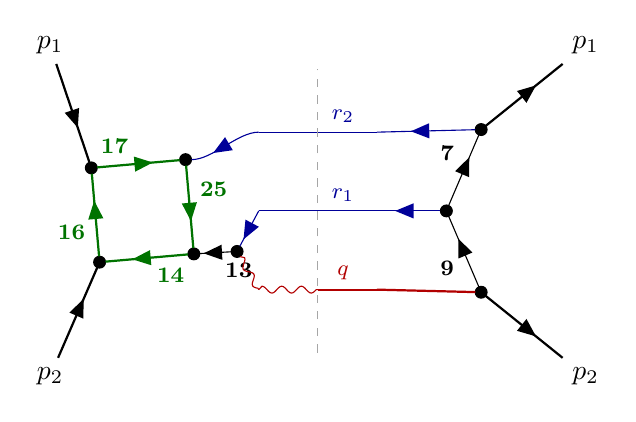
\begin{tikzpicture}
\begin{feynman}
\vertex (Lp1) at (-3.400,2.100) {$p_1$};
\vertex (Lp2) at (-3.400,-2.100) {$p_2$};
\vertex (Lcr1) at (-0.750,0.000);
\vertex (Lcr2) at (-0.750,1.000);
\vertex (Lcq) at (-0.750,-1.000);
\vertex (Mq) at (0,-1.000);
\vertex[dot] (Lv0) at (-1.574,-0.546) {};
\vertex[dot] (Lv1) at (-2.771,-0.651) {};
\vertex[dot] (Lv2) at (-2.876,0.546) {};
\vertex[dot] (Lv3) at (-1.679,0.651) {};
\vertex[dot] (Lt13) at (-1.025,-0.515) {};
\vertex (Rp1) at (3.400,2.100) {$p_1$};
\vertex (Rp2) at (3.400,-2.100) {$p_2$};
\vertex (Rcr1) at (0.750,0.000);
\vertex (Rcr2) at (0.750,1.000);
\vertex (Rcq) at (0.750,-1.000);
\vertex[dot] (R7) at (2.075,1.033) {};
\vertex[dot] (R9) at (1.633,0.000) {};
\vertex[dot] (Rroot) at (2.075,-1.033) {};
\diagram* {
(Lv0) -- [plain, thick, green!45!black, with arrow=0.55, edge label={\footnotesize\bfseries 14}] (Lv1),
(Lv1) -- [plain, thick, green!45!black, with arrow=0.55, edge label={\footnotesize\bfseries 16}] (Lv2),
(Lv2) -- [plain, thick, green!45!black, with arrow=0.55, edge label={\footnotesize\bfseries 17}] (Lv3),
(Lv3) -- [plain, thick, green!45!black, with arrow=0.55, edge label={\footnotesize\bfseries 25}] (Lv0),
(Lt13) -- [plain, with arrow=0.55, edge label={\footnotesize\bfseries 13}] (Lv0),
(Lcr1) -- [plain, blue!60!black, with arrow=0.55] (Lt13),
(Lcq) -- [boson, red!70!black] (Lt13),
(Lp2) -- [plain, thick, with arrow=0.55] (Lv1),
(Lp1) -- [plain, thick, with arrow=0.55] (Lv2),
(Lcr2) -- [plain, blue!60!black, out=180, in=0, looseness=0.75, with arrow=0.55] (Lv3),
(R9) -- [plain, with arrow=0.55, edge label={\footnotesize\bfseries 7}] (R7),
(Rroot) -- [plain, with arrow=0.55, edge label={\footnotesize\bfseries 9}] (R9),
(R7) -- [plain, thick, with arrow=0.55] (Rp1),
(Rroot) -- [plain, thick, with arrow=0.55] (Rp2),
(R9) -- [plain, blue!60!black, with arrow=0.55] (Rcr1),
(R7) -- [plain, blue!60!black, with arrow=0.55] (Rcr2),
(Rroot) -- [plain, red!70!black, double, double distance=1.2pt, thick] (Rcq),
(Rcr1) -- [plain, blue!60!black] (Lcr1),
(Rcr2) -- [plain, blue!60!black] (Lcr2),
(Rcq) -- [plain, red!70!black, double, double distance=1.2pt, thick] (Mq) -- [boson, red!70!black] (Lcq),
};
\end{feynman}
\draw[dashed, gray!70] (0,-1.80) -- (0,1.80);
\node[font=\footnotesize, blue!60!black, above] at (0.32,0.00) {$r_1$};
\node[font=\footnotesize, blue!60!black, above] at (0.32,1.00) {$r_2$};
\node[font=\footnotesize, red!70!black, above] at (0.32,-1.00) {$q$};
\end{tikzpicture}}\\[2mm]\textbf{topo1} (RR family 33, pentagon q-p2-p1-r2-r1), sector with 7 of 8 lines\\[2pt]{\footnotesize\begin{tabular}{@{}r@{\ \ }l@{\ \ }l@{}}\textbf{14} & $(k_1)^2$ & loop\\
\textbf{16} & $(k_1+p_2)^2$ & loop\\
\textbf{17} & $(k_1+p_1+p_2)^2$ & loop\\
\textbf{25} & $(k_1+p_1+p_2+r_2)^2$ & loop\\
\textbf{13} & $(p_1+p_2+r_2)^2$ & amplitude (tree on the loop)\\
\textbf{7} & $(p_1+r_2)^2$ & conjugate\\
\textbf{9} & $(p_1+r_1+r_2)^2$ & conjugate\\\end{tabular}}\\[2pt]{\scriptsize pinched: 29 = $(k_1+p_1+p_2+r_1+r_2)^2$}\end{minipage}\hfill%
\begin{minipage}[t]{0.48\textwidth}\centering\resizebox{0.9\linewidth}{!}{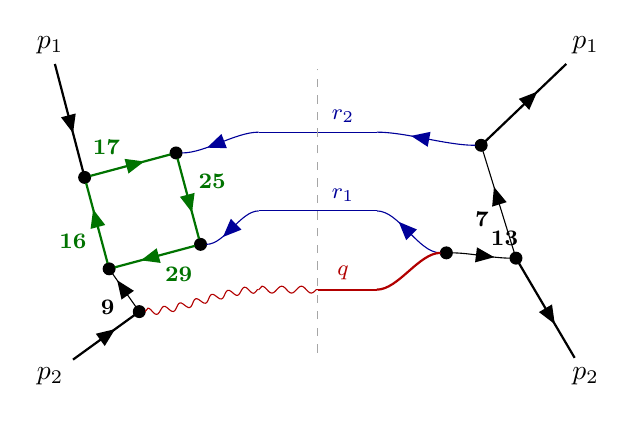
\begin{tikzpicture}
\begin{feynman}
\vertex (Lp1) at (-3.400,2.100) {$p_1$};
\vertex (Lp2) at (-3.400,-2.100) {$p_2$};
\vertex (Lcr1) at (-0.750,0.000);
\vertex (Lcr2) at (-0.750,1.000);
\vertex (Lcq) at (-0.750,-1.000);
\vertex (Mq) at (0,-1.000);
\vertex[dot] (Lv0) at (-2.650,-0.736) {};
\vertex[dot] (Lv1) at (-2.961,0.425) {};
\vertex[dot] (Lv2) at (-1.800,0.736) {};
\vertex[dot] (Lv3) at (-1.489,-0.425) {};
\vertex[dot] (Lt9) at (-2.267,-1.279) {};
\vertex (Rp1) at (3.400,2.100) {$p_1$};
\vertex (Rp2) at (3.400,-2.100) {$p_2$};
\vertex (Rcr1) at (0.750,0.000);
\vertex (Rcr2) at (0.750,1.000);
\vertex (Rcq) at (0.750,-1.000);
\vertex[dot] (R7) at (2.075,0.833) {};
\vertex[dot] (R13) at (2.517,-0.600) {};
\vertex[dot] (Rroot) at (1.633,-0.533) {};
\diagram* {
(Lv0) -- [plain, thick, green!45!black, with arrow=0.55, edge label={\footnotesize\bfseries 16}] (Lv1),
(Lv1) -- [plain, thick, green!45!black, with arrow=0.55, edge label={\footnotesize\bfseries 17}] (Lv2),
(Lv2) -- [plain, thick, green!45!black, with arrow=0.55, edge label={\footnotesize\bfseries 25}] (Lv3),
(Lv3) -- [plain, thick, green!45!black, with arrow=0.55, edge label={\footnotesize\bfseries 29}] (Lv0),
(Lt9) -- [plain, with arrow=0.55, edge label={\footnotesize\bfseries 9}] (Lv0),
(Lp2) -- [plain, thick, with arrow=0.55] (Lt9),
(Lcq) -- [boson, red!70!black, out=180, in=0, looseness=0.75] (Lt9),
(Lp1) -- [plain, thick, with arrow=0.55] (Lv1),
(Lcr2) -- [plain, blue!60!black, out=180, in=0, looseness=0.75, with arrow=0.55] (Lv2),
(Lcr1) -- [plain, blue!60!black, out=180, in=0, looseness=0.75, with arrow=0.55] (Lv3),
(R13) -- [plain, with arrow=0.55, edge label={\footnotesize\bfseries 7}] (R7),
(Rroot) -- [plain, out=0, in=180, looseness=0.75, with arrow=0.55, edge label={\footnotesize\bfseries 13}] (R13),
(R7) -- [plain, thick, with arrow=0.55] (Rp1),
(R13) -- [plain, thick, with arrow=0.55] (Rp2),
(Rroot) -- [plain, blue!60!black, out=180, in=0, looseness=0.75, with arrow=0.55] (Rcr1),
(R7) -- [plain, blue!60!black, out=180, in=0, looseness=0.75, with arrow=0.55] (Rcr2),
(Rroot) -- [plain, red!70!black, double, double distance=1.2pt, thick, out=180, in=0, looseness=0.75] (Rcq),
(Rcr1) -- [plain, blue!60!black] (Lcr1),
(Rcr2) -- [plain, blue!60!black] (Lcr2),
(Rcq) -- [plain, red!70!black, double, double distance=1.2pt, thick] (Mq) -- [boson, red!70!black] (Lcq),
};
\end{feynman}
\draw[dashed, gray!70] (0,-1.80) -- (0,1.80);
\node[font=\footnotesize, blue!60!black, above] at (0.32,0.00) {$r_1$};
\node[font=\footnotesize, blue!60!black, above] at (0.32,1.00) {$r_2$};
\node[font=\footnotesize, red!70!black, above] at (0.32,-1.00) {$q$};
\end{tikzpicture}}\\[2mm]\textbf{topo1} (RR family 33, pentagon q-p2-p1-r2-r1), sector with 7 of 8 lines\\[2pt]{\footnotesize\begin{tabular}{@{}r@{\ \ }l@{\ \ }l@{}}\textbf{16} & $(k_1+p_2)^2$ & loop\\
\textbf{17} & $(k_1+p_1+p_2)^2$ & loop\\
\textbf{25} & $(k_1+p_1+p_2+r_2)^2$ & loop\\
\textbf{29} & $(k_1+p_1+p_2+r_1+r_2)^2$ & loop\\
\textbf{9} & $(p_1+r_1+r_2)^2$ & amplitude (tree on the loop)\\
\textbf{7} & $(p_1+r_2)^2$ & conjugate\\
\textbf{13} & $(p_1+p_2+r_2)^2$ & conjugate\\\end{tabular}}\\[2pt]{\scriptsize pinched: 14 = $(k_1)^2$}\end{minipage}

\bigskip

\begin{minipage}[t]{0.48\textwidth}\centering\resizebox{0.9\linewidth}{!}{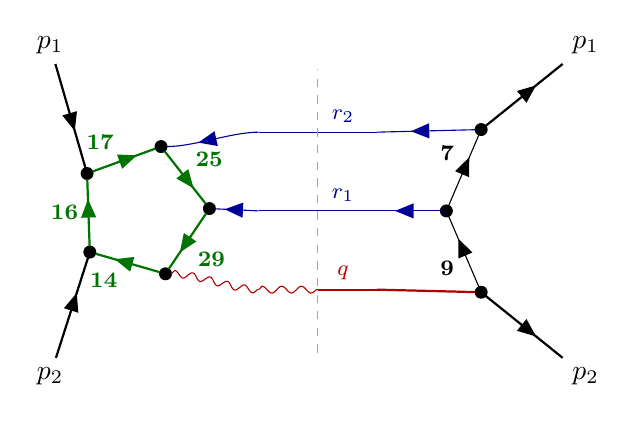
\begin{tikzpicture}
\begin{feynman}
\vertex (Lp1) at (-3.400,2.100) {$p_1$};
\vertex (Lp2) at (-3.400,-2.100) {$p_2$};
\vertex (Lcr1) at (-0.750,0.000);
\vertex (Lcr2) at (-0.750,1.000);
\vertex (Lcq) at (-0.750,-1.000);
\vertex (Mq) at (0,-1.000);
\vertex[dot] (Lv0) at (-1.934,-0.799) {};
\vertex[dot] (Lv1) at (-2.895,-0.523) {};
\vertex[dot] (Lv2) at (-2.930,0.475) {};
\vertex[dot] (Lv3) at (-1.991,0.817) {};
\vertex[dot] (Lv4) at (-1.376,0.030) {};
\vertex (Rp1) at (3.400,2.100) {$p_1$};
\vertex (Rp2) at (3.400,-2.100) {$p_2$};
\vertex (Rcr1) at (0.750,0.000);
\vertex (Rcr2) at (0.750,1.000);
\vertex (Rcq) at (0.750,-1.000);
\vertex[dot] (R7) at (2.075,1.033) {};
\vertex[dot] (R9) at (1.633,0.000) {};
\vertex[dot] (Rroot) at (2.075,-1.033) {};
\diagram* {
(Lv0) -- [plain, thick, green!45!black, with arrow=0.55, edge label={\footnotesize\bfseries 14}] (Lv1),
(Lv1) -- [plain, thick, green!45!black, with arrow=0.55, edge label={\footnotesize\bfseries 16}] (Lv2),
(Lv2) -- [plain, thick, green!45!black, with arrow=0.55, edge label={\footnotesize\bfseries 17}] (Lv3),
(Lv3) -- [plain, thick, green!45!black, with arrow=0.55, edge label={\footnotesize\bfseries 25}] (Lv4),
(Lv4) -- [plain, thick, green!45!black, with arrow=0.55, edge label={\footnotesize\bfseries 29}] (Lv0),
(Lcq) -- [boson, red!70!black, out=180, in=0, looseness=0.75] (Lv0),
(Lp2) -- [plain, thick, with arrow=0.55] (Lv1),
(Lp1) -- [plain, thick, with arrow=0.55] (Lv2),
(Lcr2) -- [plain, blue!60!black, out=180, in=0, looseness=0.75, with arrow=0.55] (Lv3),
(Lcr1) -- [plain, blue!60!black, with arrow=0.55] (Lv4),
(R9) -- [plain, with arrow=0.55, edge label={\footnotesize\bfseries 7}] (R7),
(Rroot) -- [plain, with arrow=0.55, edge label={\footnotesize\bfseries 9}] (R9),
(R7) -- [plain, thick, with arrow=0.55] (Rp1),
(Rroot) -- [plain, thick, with arrow=0.55] (Rp2),
(R9) -- [plain, blue!60!black, with arrow=0.55] (Rcr1),
(R7) -- [plain, blue!60!black, with arrow=0.55] (Rcr2),
(Rroot) -- [plain, red!70!black, double, double distance=1.2pt, thick] (Rcq),
(Rcr1) -- [plain, blue!60!black] (Lcr1),
(Rcr2) -- [plain, blue!60!black] (Lcr2),
(Rcq) -- [plain, red!70!black, double, double distance=1.2pt, thick] (Mq) -- [boson, red!70!black] (Lcq),
};
\end{feynman}
\draw[dashed, gray!70] (0,-1.80) -- (0,1.80);
\node[font=\footnotesize, blue!60!black, above] at (0.32,0.00) {$r_1$};
\node[font=\footnotesize, blue!60!black, above] at (0.32,1.00) {$r_2$};
\node[font=\footnotesize, red!70!black, above] at (0.32,-1.00) {$q$};
\end{tikzpicture}}\\[2mm]\textbf{topo1} (RR family 33, pentagon q-p2-p1-r2-r1), sector with 7 of 8 lines\\[2pt]{\footnotesize\begin{tabular}{@{}r@{\ \ }l@{\ \ }l@{}}\textbf{14} & $(k_1)^2$ & loop\\
\textbf{16} & $(k_1+p_2)^2$ & loop\\
\textbf{17} & $(k_1+p_1+p_2)^2$ & loop\\
\textbf{25} & $(k_1+p_1+p_2+r_2)^2$ & loop\\
\textbf{29} & $(k_1+p_1+p_2+r_1+r_2)^2$ & loop\\
\textbf{7} & $(p_1+r_2)^2$ & conjugate\\
\textbf{9} & $(p_1+r_1+r_2)^2$ & conjugate\\\end{tabular}}\\[2pt]{\scriptsize pinched: 13 = $(p_1+p_2+r_2)^2$}\end{minipage}\hfill%
\begin{minipage}[t]{0.48\textwidth}\centering\resizebox{0.9\linewidth}{!}{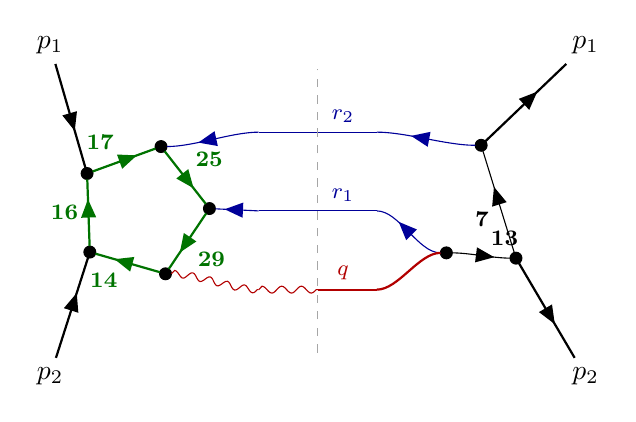
\begin{tikzpicture}
\begin{feynman}
\vertex (Lp1) at (-3.400,2.100) {$p_1$};
\vertex (Lp2) at (-3.400,-2.100) {$p_2$};
\vertex (Lcr1) at (-0.750,0.000);
\vertex (Lcr2) at (-0.750,1.000);
\vertex (Lcq) at (-0.750,-1.000);
\vertex (Mq) at (0,-1.000);
\vertex[dot] (Lv0) at (-1.934,-0.799) {};
\vertex[dot] (Lv1) at (-2.895,-0.523) {};
\vertex[dot] (Lv2) at (-2.930,0.475) {};
\vertex[dot] (Lv3) at (-1.991,0.817) {};
\vertex[dot] (Lv4) at (-1.376,0.030) {};
\vertex (Rp1) at (3.400,2.100) {$p_1$};
\vertex (Rp2) at (3.400,-2.100) {$p_2$};
\vertex (Rcr1) at (0.750,0.000);
\vertex (Rcr2) at (0.750,1.000);
\vertex (Rcq) at (0.750,-1.000);
\vertex[dot] (R7) at (2.075,0.833) {};
\vertex[dot] (R13) at (2.517,-0.600) {};
\vertex[dot] (Rroot) at (1.633,-0.533) {};
\diagram* {
(Lv0) -- [plain, thick, green!45!black, with arrow=0.55, edge label={\footnotesize\bfseries 14}] (Lv1),
(Lv1) -- [plain, thick, green!45!black, with arrow=0.55, edge label={\footnotesize\bfseries 16}] (Lv2),
(Lv2) -- [plain, thick, green!45!black, with arrow=0.55, edge label={\footnotesize\bfseries 17}] (Lv3),
(Lv3) -- [plain, thick, green!45!black, with arrow=0.55, edge label={\footnotesize\bfseries 25}] (Lv4),
(Lv4) -- [plain, thick, green!45!black, with arrow=0.55, edge label={\footnotesize\bfseries 29}] (Lv0),
(Lcq) -- [boson, red!70!black, out=180, in=0, looseness=0.75] (Lv0),
(Lp2) -- [plain, thick, with arrow=0.55] (Lv1),
(Lp1) -- [plain, thick, with arrow=0.55] (Lv2),
(Lcr2) -- [plain, blue!60!black, out=180, in=0, looseness=0.75, with arrow=0.55] (Lv3),
(Lcr1) -- [plain, blue!60!black, with arrow=0.55] (Lv4),
(R13) -- [plain, with arrow=0.55, edge label={\footnotesize\bfseries 7}] (R7),
(Rroot) -- [plain, out=0, in=180, looseness=0.75, with arrow=0.55, edge label={\footnotesize\bfseries 13}] (R13),
(R7) -- [plain, thick, with arrow=0.55] (Rp1),
(R13) -- [plain, thick, with arrow=0.55] (Rp2),
(Rroot) -- [plain, blue!60!black, out=180, in=0, looseness=0.75, with arrow=0.55] (Rcr1),
(R7) -- [plain, blue!60!black, out=180, in=0, looseness=0.75, with arrow=0.55] (Rcr2),
(Rroot) -- [plain, red!70!black, double, double distance=1.2pt, thick, out=180, in=0, looseness=0.75] (Rcq),
(Rcr1) -- [plain, blue!60!black] (Lcr1),
(Rcr2) -- [plain, blue!60!black] (Lcr2),
(Rcq) -- [plain, red!70!black, double, double distance=1.2pt, thick] (Mq) -- [boson, red!70!black] (Lcq),
};
\end{feynman}
\draw[dashed, gray!70] (0,-1.80) -- (0,1.80);
\node[font=\footnotesize, blue!60!black, above] at (0.32,0.00) {$r_1$};
\node[font=\footnotesize, blue!60!black, above] at (0.32,1.00) {$r_2$};
\node[font=\footnotesize, red!70!black, above] at (0.32,-1.00) {$q$};
\end{tikzpicture}}\\[2mm]\textbf{topo1} (RR family 33, pentagon q-p2-p1-r2-r1), sector with 7 of 8 lines\\[2pt]{\footnotesize\begin{tabular}{@{}r@{\ \ }l@{\ \ }l@{}}\textbf{14} & $(k_1)^2$ & loop\\
\textbf{16} & $(k_1+p_2)^2$ & loop\\
\textbf{17} & $(k_1+p_1+p_2)^2$ & loop\\
\textbf{25} & $(k_1+p_1+p_2+r_2)^2$ & loop\\
\textbf{29} & $(k_1+p_1+p_2+r_1+r_2)^2$ & loop\\
\textbf{7} & $(p_1+r_2)^2$ & conjugate\\
\textbf{13} & $(p_1+p_2+r_2)^2$ & conjugate\\\end{tabular}}\\[2pt]{\scriptsize pinched: 9 = $(p_1+r_1+r_2)^2$}\end{minipage}

\bigskip

\begin{minipage}[t]{0.48\textwidth}\centering\resizebox{0.9\linewidth}{!}{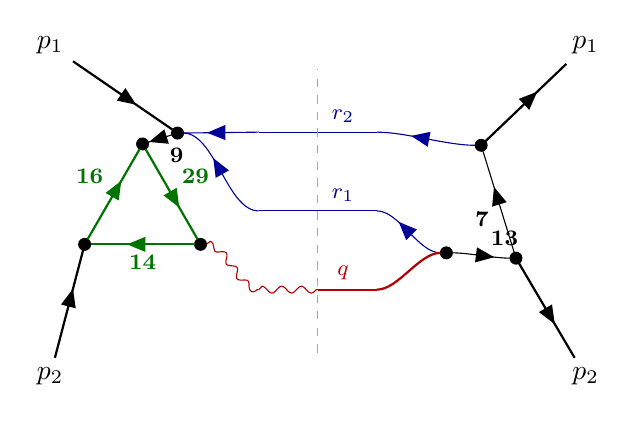
\begin{tikzpicture}
\begin{feynman}
\vertex (Lp1) at (-3.400,2.100) {$p_1$};
\vertex (Lp2) at (-3.400,-2.100) {$p_2$};
\vertex (Lcr1) at (-0.750,0.000);
\vertex (Lcr2) at (-0.750,1.000);
\vertex (Lcq) at (-0.750,-1.000);
\vertex (Mq) at (0,-1.000);
\vertex[dot] (Lv0) at (-1.489,-0.425) {};
\vertex[dot] (Lv1) at (-2.961,-0.425) {};
\vertex[dot] (Lv2) at (-2.225,0.850) {};
\vertex[dot] (Lt9) at (-1.781,0.988) {};
\vertex (Rp1) at (3.400,2.100) {$p_1$};
\vertex (Rp2) at (3.400,-2.100) {$p_2$};
\vertex (Rcr1) at (0.750,0.000);
\vertex (Rcr2) at (0.750,1.000);
\vertex (Rcq) at (0.750,-1.000);
\vertex[dot] (R7) at (2.075,0.833) {};
\vertex[dot] (R13) at (2.517,-0.600) {};
\vertex[dot] (Rroot) at (1.633,-0.533) {};
\diagram* {
(Lv0) -- [plain, thick, green!45!black, with arrow=0.55, edge label={\footnotesize\bfseries 14}] (Lv1),
(Lv1) -- [plain, thick, green!45!black, with arrow=0.55, edge label={\footnotesize\bfseries 16}] (Lv2),
(Lv2) -- [plain, thick, green!45!black, with arrow=0.55, edge label={\footnotesize\bfseries 29}] (Lv0),
(Lcq) -- [boson, red!70!black, out=180, in=0, looseness=0.75] (Lv0),
(Lp2) -- [plain, thick, with arrow=0.55] (Lv1),
(Lt9) -- [plain, with arrow=0.55, edge label={\footnotesize\bfseries 9}] (Lv2),
(Lcr1) -- [plain, blue!60!black, out=180, in=0, looseness=0.75, with arrow=0.55] (Lt9),
(Lcr2) -- [plain, blue!60!black, with arrow=0.55] (Lt9),
(Lp1) -- [plain, thick, with arrow=0.55] (Lt9),
(R13) -- [plain, with arrow=0.55, edge label={\footnotesize\bfseries 7}] (R7),
(Rroot) -- [plain, out=0, in=180, looseness=0.75, with arrow=0.55, edge label={\footnotesize\bfseries 13}] (R13),
(R7) -- [plain, thick, with arrow=0.55] (Rp1),
(R13) -- [plain, thick, with arrow=0.55] (Rp2),
(Rroot) -- [plain, blue!60!black, out=180, in=0, looseness=0.75, with arrow=0.55] (Rcr1),
(R7) -- [plain, blue!60!black, out=180, in=0, looseness=0.75, with arrow=0.55] (Rcr2),
(Rroot) -- [plain, red!70!black, double, double distance=1.2pt, thick, out=180, in=0, looseness=0.75] (Rcq),
(Rcr1) -- [plain, blue!60!black] (Lcr1),
(Rcr2) -- [plain, blue!60!black] (Lcr2),
(Rcq) -- [plain, red!70!black, double, double distance=1.2pt, thick] (Mq) -- [boson, red!70!black] (Lcq),
};
\end{feynman}
\draw[dashed, gray!70] (0,-1.80) -- (0,1.80);
\node[font=\footnotesize, blue!60!black, above] at (0.32,0.00) {$r_1$};
\node[font=\footnotesize, blue!60!black, above] at (0.32,1.00) {$r_2$};
\node[font=\footnotesize, red!70!black, above] at (0.32,-1.00) {$q$};
\end{tikzpicture}}\\[2mm]\textbf{topo1} (RR family 33, pentagon q-p2-p1-r2-r1), sector with 6 of 8 lines\\[2pt]{\footnotesize\begin{tabular}{@{}r@{\ \ }l@{\ \ }l@{}}\textbf{14} & $(k_1)^2$ & loop\\
\textbf{16} & $(k_1+p_2)^2$ & loop\\
\textbf{29} & $(k_1+p_1+p_2+r_1+r_2)^2$ & loop\\
\textbf{9} & $(p_1+r_1+r_2)^2$ & amplitude (tree on the loop)\\
\textbf{7} & $(p_1+r_2)^2$ & conjugate\\
\textbf{13} & $(p_1+p_2+r_2)^2$ & conjugate\\\end{tabular}}\\[2pt]{\scriptsize pinched: 17 = $(k_1+p_1+p_2)^2$, 25 = $(k_1+p_1+p_2+r_2)^2$}\end{minipage}\hfill%
\begin{minipage}[t]{0.48\textwidth}\centering\resizebox{0.9\linewidth}{!}{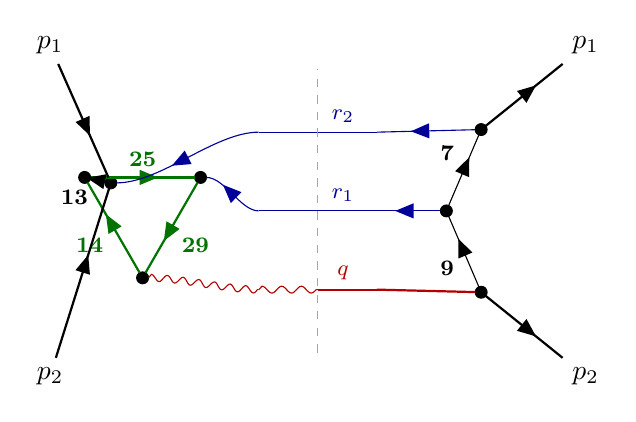
\begin{tikzpicture}
\begin{feynman}
\vertex (Lp1) at (-3.400,2.100) {$p_1$};
\vertex (Lp2) at (-3.400,-2.100) {$p_2$};
\vertex (Lcr1) at (-0.750,0.000);
\vertex (Lcr2) at (-0.750,1.000);
\vertex (Lcq) at (-0.750,-1.000);
\vertex (Mq) at (0,-1.000);
\vertex[dot] (Lv0) at (-2.225,-0.850) {};
\vertex[dot] (Lv1) at (-2.961,0.425) {};
\vertex[dot] (Lv2) at (-1.489,0.425) {};
\vertex[dot] (Lt13) at (-2.628,0.356) {};
\vertex (Rp1) at (3.400,2.100) {$p_1$};
\vertex (Rp2) at (3.400,-2.100) {$p_2$};
\vertex (Rcr1) at (0.750,0.000);
\vertex (Rcr2) at (0.750,1.000);
\vertex (Rcq) at (0.750,-1.000);
\vertex[dot] (R7) at (2.075,1.033) {};
\vertex[dot] (R9) at (1.633,0.000) {};
\vertex[dot] (Rroot) at (2.075,-1.033) {};
\diagram* {
(Lv0) -- [plain, thick, green!45!black, with arrow=0.55, edge label={\footnotesize\bfseries 14}] (Lv1),
(Lv1) -- [plain, thick, green!45!black, with arrow=0.55, edge label={\footnotesize\bfseries 25}] (Lv2),
(Lv2) -- [plain, thick, green!45!black, with arrow=0.55, edge label={\footnotesize\bfseries 29}] (Lv0),
(Lcq) -- [boson, red!70!black, out=180, in=0, looseness=0.75] (Lv0),
(Lt13) -- [plain, with arrow=0.55, edge label={\footnotesize\bfseries 13}] (Lv1),
(Lp2) -- [plain, thick, with arrow=0.55] (Lt13),
(Lcr2) -- [plain, blue!60!black, out=180, in=0, looseness=0.75, with arrow=0.55] (Lt13),
(Lp1) -- [plain, thick, with arrow=0.55] (Lt13),
(Lcr1) -- [plain, blue!60!black, out=180, in=0, looseness=0.75, with arrow=0.55] (Lv2),
(R9) -- [plain, with arrow=0.55, edge label={\footnotesize\bfseries 7}] (R7),
(Rroot) -- [plain, with arrow=0.55, edge label={\footnotesize\bfseries 9}] (R9),
(R7) -- [plain, thick, with arrow=0.55] (Rp1),
(Rroot) -- [plain, thick, with arrow=0.55] (Rp2),
(R9) -- [plain, blue!60!black, with arrow=0.55] (Rcr1),
(R7) -- [plain, blue!60!black, with arrow=0.55] (Rcr2),
(Rroot) -- [plain, red!70!black, double, double distance=1.2pt, thick] (Rcq),
(Rcr1) -- [plain, blue!60!black] (Lcr1),
(Rcr2) -- [plain, blue!60!black] (Lcr2),
(Rcq) -- [plain, red!70!black, double, double distance=1.2pt, thick] (Mq) -- [boson, red!70!black] (Lcq),
};
\end{feynman}
\draw[dashed, gray!70] (0,-1.80) -- (0,1.80);
\node[font=\footnotesize, blue!60!black, above] at (0.32,0.00) {$r_1$};
\node[font=\footnotesize, blue!60!black, above] at (0.32,1.00) {$r_2$};
\node[font=\footnotesize, red!70!black, above] at (0.32,-1.00) {$q$};
\end{tikzpicture}}\\[2mm]\textbf{topo1} (RR family 33, pentagon q-p2-p1-r2-r1), sector with 6 of 8 lines\\[2pt]{\footnotesize\begin{tabular}{@{}r@{\ \ }l@{\ \ }l@{}}\textbf{14} & $(k_1)^2$ & loop\\
\textbf{25} & $(k_1+p_1+p_2+r_2)^2$ & loop\\
\textbf{29} & $(k_1+p_1+p_2+r_1+r_2)^2$ & loop\\
\textbf{13} & $(p_1+p_2+r_2)^2$ & amplitude (tree on the loop)\\
\textbf{7} & $(p_1+r_2)^2$ & conjugate\\
\textbf{9} & $(p_1+r_1+r_2)^2$ & conjugate\\\end{tabular}}\\[2pt]{\scriptsize pinched: 16 = $(k_1+p_2)^2$, 17 = $(k_1+p_1+p_2)^2$}\end{minipage}

\bigskip

\begin{minipage}[t]{0.48\textwidth}\centering\resizebox{0.9\linewidth}{!}{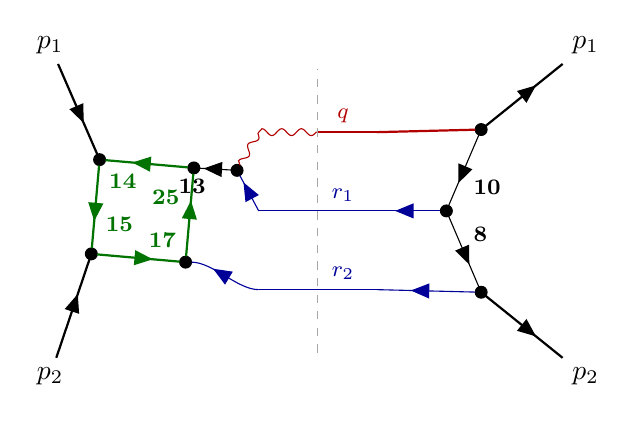
\begin{tikzpicture}
\begin{feynman}
\vertex (Lp1) at (-3.400,2.100) {$p_1$};
\vertex (Lp2) at (-3.400,-2.100) {$p_2$};
\vertex (Lcr1) at (-0.750,0.000);
\vertex (Lcr2) at (-0.750,-1.000);
\vertex (Lcq) at (-0.750,1.000);
\vertex (Mq) at (0,1.000);
\vertex[dot] (Lv0) at (-1.574,0.546) {};
\vertex[dot] (Lv1) at (-2.771,0.651) {};
\vertex[dot] (Lv2) at (-2.876,-0.546) {};
\vertex[dot] (Lv3) at (-1.679,-0.651) {};
\vertex[dot] (Lt13) at (-1.025,0.515) {};
\vertex (Rp1) at (3.400,2.100) {$p_1$};
\vertex (Rp2) at (3.400,-2.100) {$p_2$};
\vertex (Rcr1) at (0.750,0.000);
\vertex (Rcr2) at (0.750,-1.000);
\vertex (Rcq) at (0.750,1.000);
\vertex[dot] (R8) at (2.075,-1.033) {};
\vertex[dot] (R10) at (1.633,0.000) {};
\vertex[dot] (Rroot) at (2.075,1.033) {};
\diagram* {
(Lv0) -- [plain, thick, green!45!black, with arrow=0.55, edge label={\footnotesize\bfseries 14}] (Lv1),
(Lv1) -- [plain, thick, green!45!black, with arrow=0.55, edge label={\footnotesize\bfseries 15}] (Lv2),
(Lv2) -- [plain, thick, green!45!black, with arrow=0.55, edge label={\footnotesize\bfseries 17}] (Lv3),
(Lv3) -- [plain, thick, green!45!black, with arrow=0.55, edge label={\footnotesize\bfseries 25}] (Lv0),
(Lt13) -- [plain, with arrow=0.55, edge label={\footnotesize\bfseries 13}] (Lv0),
(Lcr1) -- [plain, blue!60!black, with arrow=0.55] (Lt13),
(Lcq) -- [boson, red!70!black] (Lt13),
(Lp1) -- [plain, thick, with arrow=0.55] (Lv1),
(Lp2) -- [plain, thick, with arrow=0.55] (Lv2),
(Lcr2) -- [plain, blue!60!black, out=180, in=0, looseness=0.75, with arrow=0.55] (Lv3),
(R10) -- [plain, with arrow=0.55, edge label={\footnotesize\bfseries 8}] (R8),
(Rroot) -- [plain, with arrow=0.55, edge label={\footnotesize\bfseries 10}] (R10),
(Rroot) -- [plain, thick, with arrow=0.55] (Rp1),
(R8) -- [plain, thick, with arrow=0.55] (Rp2),
(R10) -- [plain, blue!60!black, with arrow=0.55] (Rcr1),
(R8) -- [plain, blue!60!black, with arrow=0.55] (Rcr2),
(Rroot) -- [plain, red!70!black, double, double distance=1.2pt, thick] (Rcq),
(Rcr1) -- [plain, blue!60!black] (Lcr1),
(Rcr2) -- [plain, blue!60!black] (Lcr2),
(Rcq) -- [plain, red!70!black, double, double distance=1.2pt, thick] (Mq) -- [boson, red!70!black] (Lcq),
};
\end{feynman}
\draw[dashed, gray!70] (0,-1.80) -- (0,1.80);
\node[font=\footnotesize, blue!60!black, above] at (0.32,0.00) {$r_1$};
\node[font=\footnotesize, blue!60!black, above] at (0.32,-1.00) {$r_2$};
\node[font=\footnotesize, red!70!black, above] at (0.32,1.00) {$q$};
\end{tikzpicture}}\\[2mm]\textbf{topo2} (RR family 29, pentagon q-p1-p2-r2-r1), sector with 7 of 8 lines\\[2pt]{\footnotesize\begin{tabular}{@{}r@{\ \ }l@{\ \ }l@{}}\textbf{14} & $(k_1)^2$ & loop\\
\textbf{15} & $(k_1+p_1)^2$ & loop\\
\textbf{17} & $(k_1+p_1+p_2)^2$ & loop\\
\textbf{25} & $(k_1+p_1+p_2+r_2)^2$ & loop\\
\textbf{13} & $(p_1+p_2+r_2)^2$ & amplitude (tree on the loop)\\
\textbf{8} & $(p_2+r_2)^2$ & conjugate\\
\textbf{10} & $(p_2+r_1+r_2)^2$ & conjugate\\\end{tabular}}\\[2pt]{\scriptsize pinched: 29 = $(k_1+p_1+p_2+r_1+r_2)^2$}\end{minipage}\hfill%
\begin{minipage}[t]{0.48\textwidth}\centering\resizebox{0.9\linewidth}{!}{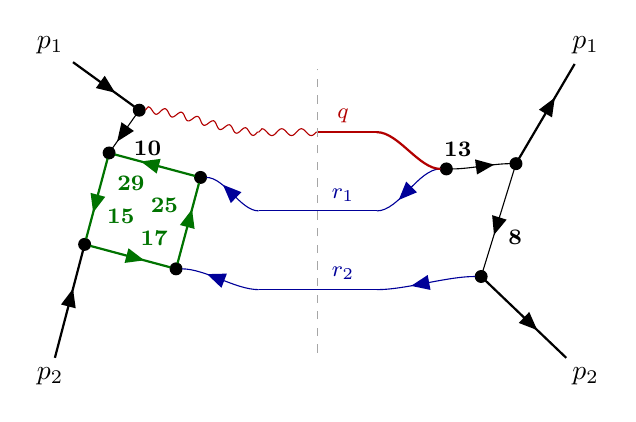
\begin{tikzpicture}
\begin{feynman}
\vertex (Lp1) at (-3.400,2.100) {$p_1$};
\vertex (Lp2) at (-3.400,-2.100) {$p_2$};
\vertex (Lcr1) at (-0.750,0.000);
\vertex (Lcr2) at (-0.750,-1.000);
\vertex (Lcq) at (-0.750,1.000);
\vertex (Mq) at (0,1.000);
\vertex[dot] (Lv0) at (-2.650,0.736) {};
\vertex[dot] (Lv1) at (-2.961,-0.425) {};
\vertex[dot] (Lv2) at (-1.800,-0.736) {};
\vertex[dot] (Lv3) at (-1.489,0.425) {};
\vertex[dot] (Lt10) at (-2.267,1.279) {};
\vertex (Rp1) at (3.400,2.100) {$p_1$};
\vertex (Rp2) at (3.400,-2.100) {$p_2$};
\vertex (Rcr1) at (0.750,0.000);
\vertex (Rcr2) at (0.750,-1.000);
\vertex (Rcq) at (0.750,1.000);
\vertex[dot] (R8) at (2.075,-0.833) {};
\vertex[dot] (R13) at (2.517,0.600) {};
\vertex[dot] (Rroot) at (1.633,0.533) {};
\diagram* {
(Lv0) -- [plain, thick, green!45!black, with arrow=0.55, edge label={\footnotesize\bfseries 15}] (Lv1),
(Lv1) -- [plain, thick, green!45!black, with arrow=0.55, edge label={\footnotesize\bfseries 17}] (Lv2),
(Lv2) -- [plain, thick, green!45!black, with arrow=0.55, edge label={\footnotesize\bfseries 25}] (Lv3),
(Lv3) -- [plain, thick, green!45!black, with arrow=0.55, edge label={\footnotesize\bfseries 29}] (Lv0),
(Lt10) -- [plain, with arrow=0.55, edge label={\footnotesize\bfseries 10}] (Lv0),
(Lcq) -- [boson, red!70!black, out=180, in=0, looseness=0.75] (Lt10),
(Lp1) -- [plain, thick, with arrow=0.55] (Lt10),
(Lp2) -- [plain, thick, with arrow=0.55] (Lv1),
(Lcr2) -- [plain, blue!60!black, out=180, in=0, looseness=0.75, with arrow=0.55] (Lv2),
(Lcr1) -- [plain, blue!60!black, out=180, in=0, looseness=0.75, with arrow=0.55] (Lv3),
(R13) -- [plain, with arrow=0.55, edge label={\footnotesize\bfseries 8}] (R8),
(Rroot) -- [plain, out=0, in=180, looseness=0.75, with arrow=0.55, edge label={\footnotesize\bfseries 13}] (R13),
(R13) -- [plain, thick, with arrow=0.55] (Rp1),
(R8) -- [plain, thick, with arrow=0.55] (Rp2),
(Rroot) -- [plain, blue!60!black, out=180, in=0, looseness=0.75, with arrow=0.55] (Rcr1),
(R8) -- [plain, blue!60!black, out=180, in=0, looseness=0.75, with arrow=0.55] (Rcr2),
(Rroot) -- [plain, red!70!black, double, double distance=1.2pt, thick, out=180, in=0, looseness=0.75] (Rcq),
(Rcr1) -- [plain, blue!60!black] (Lcr1),
(Rcr2) -- [plain, blue!60!black] (Lcr2),
(Rcq) -- [plain, red!70!black, double, double distance=1.2pt, thick] (Mq) -- [boson, red!70!black] (Lcq),
};
\end{feynman}
\draw[dashed, gray!70] (0,-1.80) -- (0,1.80);
\node[font=\footnotesize, blue!60!black, above] at (0.32,0.00) {$r_1$};
\node[font=\footnotesize, blue!60!black, above] at (0.32,-1.00) {$r_2$};
\node[font=\footnotesize, red!70!black, above] at (0.32,1.00) {$q$};
\end{tikzpicture}}\\[2mm]\textbf{topo2} (RR family 29, pentagon q-p1-p2-r2-r1), sector with 7 of 8 lines\\[2pt]{\footnotesize\begin{tabular}{@{}r@{\ \ }l@{\ \ }l@{}}\textbf{15} & $(k_1+p_1)^2$ & loop\\
\textbf{17} & $(k_1+p_1+p_2)^2$ & loop\\
\textbf{25} & $(k_1+p_1+p_2+r_2)^2$ & loop\\
\textbf{29} & $(k_1+p_1+p_2+r_1+r_2)^2$ & loop\\
\textbf{10} & $(p_2+r_1+r_2)^2$ & amplitude (tree on the loop)\\
\textbf{8} & $(p_2+r_2)^2$ & conjugate\\
\textbf{13} & $(p_1+p_2+r_2)^2$ & conjugate\\\end{tabular}}\\[2pt]{\scriptsize pinched: 14 = $(k_1)^2$}\end{minipage}

\bigskip

\begin{minipage}[t]{0.48\textwidth}\centering\resizebox{0.9\linewidth}{!}{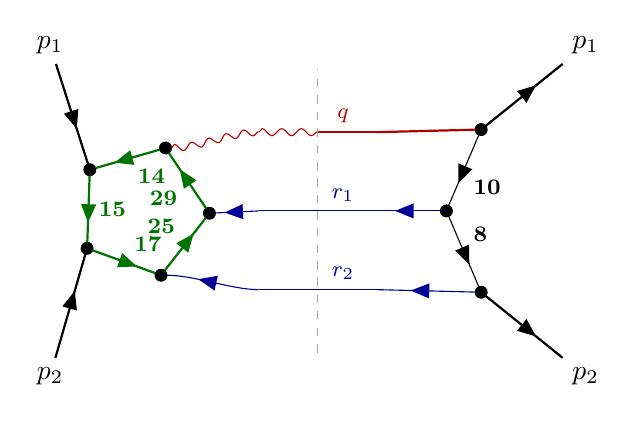
\begin{tikzpicture}
\begin{feynman}
\vertex (Lp1) at (-3.400,2.100) {$p_1$};
\vertex (Lp2) at (-3.400,-2.100) {$p_2$};
\vertex (Lcr1) at (-0.750,0.000);
\vertex (Lcr2) at (-0.750,-1.000);
\vertex (Lcq) at (-0.750,1.000);
\vertex (Mq) at (0,1.000);
\vertex[dot] (Lv0) at (-1.934,0.799) {};
\vertex[dot] (Lv1) at (-2.895,0.523) {};
\vertex[dot] (Lv2) at (-2.930,-0.475) {};
\vertex[dot] (Lv3) at (-1.991,-0.817) {};
\vertex[dot] (Lv4) at (-1.376,-0.030) {};
\vertex (Rp1) at (3.400,2.100) {$p_1$};
\vertex (Rp2) at (3.400,-2.100) {$p_2$};
\vertex (Rcr1) at (0.750,0.000);
\vertex (Rcr2) at (0.750,-1.000);
\vertex (Rcq) at (0.750,1.000);
\vertex[dot] (R8) at (2.075,-1.033) {};
\vertex[dot] (R10) at (1.633,0.000) {};
\vertex[dot] (Rroot) at (2.075,1.033) {};
\diagram* {
(Lv0) -- [plain, thick, green!45!black, with arrow=0.55, edge label={\footnotesize\bfseries 14}] (Lv1),
(Lv1) -- [plain, thick, green!45!black, with arrow=0.55, edge label={\footnotesize\bfseries 15}] (Lv2),
(Lv2) -- [plain, thick, green!45!black, with arrow=0.55, edge label={\footnotesize\bfseries 17}] (Lv3),
(Lv3) -- [plain, thick, green!45!black, with arrow=0.55, edge label={\footnotesize\bfseries 25}] (Lv4),
(Lv4) -- [plain, thick, green!45!black, with arrow=0.55, edge label={\footnotesize\bfseries 29}] (Lv0),
(Lcq) -- [boson, red!70!black, out=180, in=0, looseness=0.75] (Lv0),
(Lp1) -- [plain, thick, with arrow=0.55] (Lv1),
(Lp2) -- [plain, thick, with arrow=0.55] (Lv2),
(Lcr2) -- [plain, blue!60!black, out=180, in=0, looseness=0.75, with arrow=0.55] (Lv3),
(Lcr1) -- [plain, blue!60!black, with arrow=0.55] (Lv4),
(R10) -- [plain, with arrow=0.55, edge label={\footnotesize\bfseries 8}] (R8),
(Rroot) -- [plain, with arrow=0.55, edge label={\footnotesize\bfseries 10}] (R10),
(Rroot) -- [plain, thick, with arrow=0.55] (Rp1),
(R8) -- [plain, thick, with arrow=0.55] (Rp2),
(R10) -- [plain, blue!60!black, with arrow=0.55] (Rcr1),
(R8) -- [plain, blue!60!black, with arrow=0.55] (Rcr2),
(Rroot) -- [plain, red!70!black, double, double distance=1.2pt, thick] (Rcq),
(Rcr1) -- [plain, blue!60!black] (Lcr1),
(Rcr2) -- [plain, blue!60!black] (Lcr2),
(Rcq) -- [plain, red!70!black, double, double distance=1.2pt, thick] (Mq) -- [boson, red!70!black] (Lcq),
};
\end{feynman}
\draw[dashed, gray!70] (0,-1.80) -- (0,1.80);
\node[font=\footnotesize, blue!60!black, above] at (0.32,0.00) {$r_1$};
\node[font=\footnotesize, blue!60!black, above] at (0.32,-1.00) {$r_2$};
\node[font=\footnotesize, red!70!black, above] at (0.32,1.00) {$q$};
\end{tikzpicture}}\\[2mm]\textbf{topo2} (RR family 29, pentagon q-p1-p2-r2-r1), sector with 7 of 8 lines\\[2pt]{\footnotesize\begin{tabular}{@{}r@{\ \ }l@{\ \ }l@{}}\textbf{14} & $(k_1)^2$ & loop\\
\textbf{15} & $(k_1+p_1)^2$ & loop\\
\textbf{17} & $(k_1+p_1+p_2)^2$ & loop\\
\textbf{25} & $(k_1+p_1+p_2+r_2)^2$ & loop\\
\textbf{29} & $(k_1+p_1+p_2+r_1+r_2)^2$ & loop\\
\textbf{8} & $(p_2+r_2)^2$ & conjugate\\
\textbf{10} & $(p_2+r_1+r_2)^2$ & conjugate\\\end{tabular}}\\[2pt]{\scriptsize pinched: 13 = $(p_1+p_2+r_2)^2$}\end{minipage}\hfill%
\begin{minipage}[t]{0.48\textwidth}\centering\resizebox{0.9\linewidth}{!}{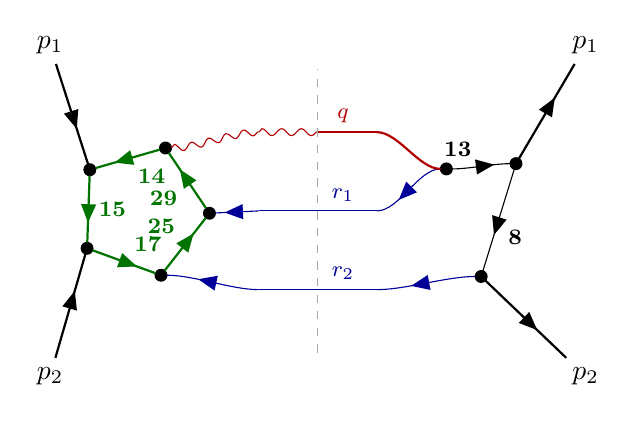
\begin{tikzpicture}
\begin{feynman}
\vertex (Lp1) at (-3.400,2.100) {$p_1$};
\vertex (Lp2) at (-3.400,-2.100) {$p_2$};
\vertex (Lcr1) at (-0.750,0.000);
\vertex (Lcr2) at (-0.750,-1.000);
\vertex (Lcq) at (-0.750,1.000);
\vertex (Mq) at (0,1.000);
\vertex[dot] (Lv0) at (-1.934,0.799) {};
\vertex[dot] (Lv1) at (-2.895,0.523) {};
\vertex[dot] (Lv2) at (-2.930,-0.475) {};
\vertex[dot] (Lv3) at (-1.991,-0.817) {};
\vertex[dot] (Lv4) at (-1.376,-0.030) {};
\vertex (Rp1) at (3.400,2.100) {$p_1$};
\vertex (Rp2) at (3.400,-2.100) {$p_2$};
\vertex (Rcr1) at (0.750,0.000);
\vertex (Rcr2) at (0.750,-1.000);
\vertex (Rcq) at (0.750,1.000);
\vertex[dot] (R8) at (2.075,-0.833) {};
\vertex[dot] (R13) at (2.517,0.600) {};
\vertex[dot] (Rroot) at (1.633,0.533) {};
\diagram* {
(Lv0) -- [plain, thick, green!45!black, with arrow=0.55, edge label={\footnotesize\bfseries 14}] (Lv1),
(Lv1) -- [plain, thick, green!45!black, with arrow=0.55, edge label={\footnotesize\bfseries 15}] (Lv2),
(Lv2) -- [plain, thick, green!45!black, with arrow=0.55, edge label={\footnotesize\bfseries 17}] (Lv3),
(Lv3) -- [plain, thick, green!45!black, with arrow=0.55, edge label={\footnotesize\bfseries 25}] (Lv4),
(Lv4) -- [plain, thick, green!45!black, with arrow=0.55, edge label={\footnotesize\bfseries 29}] (Lv0),
(Lcq) -- [boson, red!70!black, out=180, in=0, looseness=0.75] (Lv0),
(Lp1) -- [plain, thick, with arrow=0.55] (Lv1),
(Lp2) -- [plain, thick, with arrow=0.55] (Lv2),
(Lcr2) -- [plain, blue!60!black, out=180, in=0, looseness=0.75, with arrow=0.55] (Lv3),
(Lcr1) -- [plain, blue!60!black, with arrow=0.55] (Lv4),
(R13) -- [plain, with arrow=0.55, edge label={\footnotesize\bfseries 8}] (R8),
(Rroot) -- [plain, out=0, in=180, looseness=0.75, with arrow=0.55, edge label={\footnotesize\bfseries 13}] (R13),
(R13) -- [plain, thick, with arrow=0.55] (Rp1),
(R8) -- [plain, thick, with arrow=0.55] (Rp2),
(Rroot) -- [plain, blue!60!black, out=180, in=0, looseness=0.75, with arrow=0.55] (Rcr1),
(R8) -- [plain, blue!60!black, out=180, in=0, looseness=0.75, with arrow=0.55] (Rcr2),
(Rroot) -- [plain, red!70!black, double, double distance=1.2pt, thick, out=180, in=0, looseness=0.75] (Rcq),
(Rcr1) -- [plain, blue!60!black] (Lcr1),
(Rcr2) -- [plain, blue!60!black] (Lcr2),
(Rcq) -- [plain, red!70!black, double, double distance=1.2pt, thick] (Mq) -- [boson, red!70!black] (Lcq),
};
\end{feynman}
\draw[dashed, gray!70] (0,-1.80) -- (0,1.80);
\node[font=\footnotesize, blue!60!black, above] at (0.32,0.00) {$r_1$};
\node[font=\footnotesize, blue!60!black, above] at (0.32,-1.00) {$r_2$};
\node[font=\footnotesize, red!70!black, above] at (0.32,1.00) {$q$};
\end{tikzpicture}}\\[2mm]\textbf{topo2} (RR family 29, pentagon q-p1-p2-r2-r1), sector with 7 of 8 lines\\[2pt]{\footnotesize\begin{tabular}{@{}r@{\ \ }l@{\ \ }l@{}}\textbf{14} & $(k_1)^2$ & loop\\
\textbf{15} & $(k_1+p_1)^2$ & loop\\
\textbf{17} & $(k_1+p_1+p_2)^2$ & loop\\
\textbf{25} & $(k_1+p_1+p_2+r_2)^2$ & loop\\
\textbf{29} & $(k_1+p_1+p_2+r_1+r_2)^2$ & loop\\
\textbf{8} & $(p_2+r_2)^2$ & conjugate\\
\textbf{13} & $(p_1+p_2+r_2)^2$ & conjugate\\\end{tabular}}\\[2pt]{\scriptsize pinched: 10 = $(p_2+r_1+r_2)^2$}\end{minipage}

\bigskip

\begin{minipage}[t]{0.48\textwidth}\centering\resizebox{0.9\linewidth}{!}{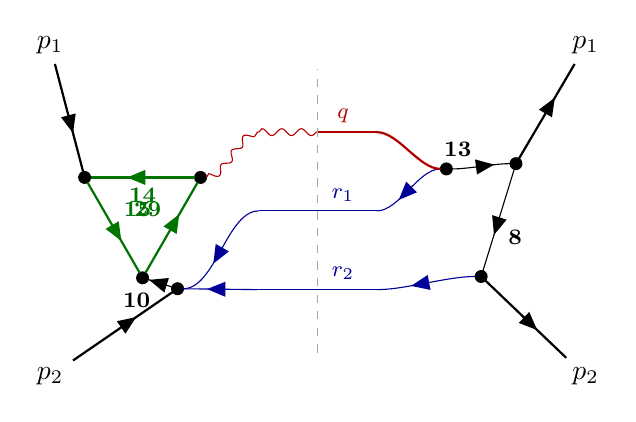
\begin{tikzpicture}
\begin{feynman}
\vertex (Lp1) at (-3.400,2.100) {$p_1$};
\vertex (Lp2) at (-3.400,-2.100) {$p_2$};
\vertex (Lcr1) at (-0.750,0.000);
\vertex (Lcr2) at (-0.750,-1.000);
\vertex (Lcq) at (-0.750,1.000);
\vertex (Mq) at (0,1.000);
\vertex[dot] (Lv0) at (-1.489,0.425) {};
\vertex[dot] (Lv1) at (-2.961,0.425) {};
\vertex[dot] (Lv2) at (-2.225,-0.850) {};
\vertex[dot] (Lt10) at (-1.781,-0.988) {};
\vertex (Rp1) at (3.400,2.100) {$p_1$};
\vertex (Rp2) at (3.400,-2.100) {$p_2$};
\vertex (Rcr1) at (0.750,0.000);
\vertex (Rcr2) at (0.750,-1.000);
\vertex (Rcq) at (0.750,1.000);
\vertex[dot] (R8) at (2.075,-0.833) {};
\vertex[dot] (R13) at (2.517,0.600) {};
\vertex[dot] (Rroot) at (1.633,0.533) {};
\diagram* {
(Lv0) -- [plain, thick, green!45!black, with arrow=0.55, edge label={\footnotesize\bfseries 14}] (Lv1),
(Lv1) -- [plain, thick, green!45!black, with arrow=0.55, edge label={\footnotesize\bfseries 15}] (Lv2),
(Lv2) -- [plain, thick, green!45!black, with arrow=0.55, edge label={\footnotesize\bfseries 29}] (Lv0),
(Lcq) -- [boson, red!70!black, out=180, in=0, looseness=0.75] (Lv0),
(Lp1) -- [plain, thick, with arrow=0.55] (Lv1),
(Lt10) -- [plain, with arrow=0.55, edge label={\footnotesize\bfseries 10}] (Lv2),
(Lp2) -- [plain, thick, with arrow=0.55] (Lt10),
(Lcr1) -- [plain, blue!60!black, out=180, in=0, looseness=0.75, with arrow=0.55] (Lt10),
(Lcr2) -- [plain, blue!60!black, with arrow=0.55] (Lt10),
(R13) -- [plain, with arrow=0.55, edge label={\footnotesize\bfseries 8}] (R8),
(Rroot) -- [plain, out=0, in=180, looseness=0.75, with arrow=0.55, edge label={\footnotesize\bfseries 13}] (R13),
(R13) -- [plain, thick, with arrow=0.55] (Rp1),
(R8) -- [plain, thick, with arrow=0.55] (Rp2),
(Rroot) -- [plain, blue!60!black, out=180, in=0, looseness=0.75, with arrow=0.55] (Rcr1),
(R8) -- [plain, blue!60!black, out=180, in=0, looseness=0.75, with arrow=0.55] (Rcr2),
(Rroot) -- [plain, red!70!black, double, double distance=1.2pt, thick, out=180, in=0, looseness=0.75] (Rcq),
(Rcr1) -- [plain, blue!60!black] (Lcr1),
(Rcr2) -- [plain, blue!60!black] (Lcr2),
(Rcq) -- [plain, red!70!black, double, double distance=1.2pt, thick] (Mq) -- [boson, red!70!black] (Lcq),
};
\end{feynman}
\draw[dashed, gray!70] (0,-1.80) -- (0,1.80);
\node[font=\footnotesize, blue!60!black, above] at (0.32,0.00) {$r_1$};
\node[font=\footnotesize, blue!60!black, above] at (0.32,-1.00) {$r_2$};
\node[font=\footnotesize, red!70!black, above] at (0.32,1.00) {$q$};
\end{tikzpicture}}\\[2mm]\textbf{topo2} (RR family 29, pentagon q-p1-p2-r2-r1), sector with 6 of 8 lines\\[2pt]{\footnotesize\begin{tabular}{@{}r@{\ \ }l@{\ \ }l@{}}\textbf{14} & $(k_1)^2$ & loop\\
\textbf{15} & $(k_1+p_1)^2$ & loop\\
\textbf{29} & $(k_1+p_1+p_2+r_1+r_2)^2$ & loop\\
\textbf{10} & $(p_2+r_1+r_2)^2$ & amplitude (tree on the loop)\\
\textbf{8} & $(p_2+r_2)^2$ & conjugate\\
\textbf{13} & $(p_1+p_2+r_2)^2$ & conjugate\\\end{tabular}}\\[2pt]{\scriptsize pinched: 17 = $(k_1+p_1+p_2)^2$, 25 = $(k_1+p_1+p_2+r_2)^2$}\end{minipage}\hfill%
\begin{minipage}[t]{0.48\textwidth}\centering\resizebox{0.9\linewidth}{!}{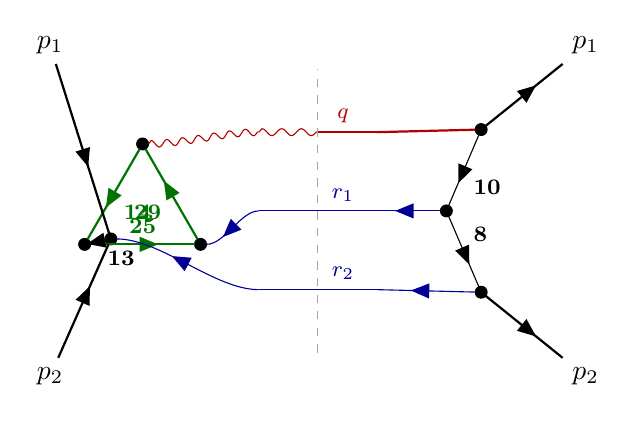
\begin{tikzpicture}
\begin{feynman}
\vertex (Lp1) at (-3.400,2.100) {$p_1$};
\vertex (Lp2) at (-3.400,-2.100) {$p_2$};
\vertex (Lcr1) at (-0.750,0.000);
\vertex (Lcr2) at (-0.750,-1.000);
\vertex (Lcq) at (-0.750,1.000);
\vertex (Mq) at (0,1.000);
\vertex[dot] (Lv0) at (-2.225,0.850) {};
\vertex[dot] (Lv1) at (-2.961,-0.425) {};
\vertex[dot] (Lv2) at (-1.489,-0.425) {};
\vertex[dot] (Lt13) at (-2.628,-0.356) {};
\vertex (Rp1) at (3.400,2.100) {$p_1$};
\vertex (Rp2) at (3.400,-2.100) {$p_2$};
\vertex (Rcr1) at (0.750,0.000);
\vertex (Rcr2) at (0.750,-1.000);
\vertex (Rcq) at (0.750,1.000);
\vertex[dot] (R8) at (2.075,-1.033) {};
\vertex[dot] (R10) at (1.633,0.000) {};
\vertex[dot] (Rroot) at (2.075,1.033) {};
\diagram* {
(Lv0) -- [plain, thick, green!45!black, with arrow=0.55, edge label={\footnotesize\bfseries 14}] (Lv1),
(Lv1) -- [plain, thick, green!45!black, with arrow=0.55, edge label={\footnotesize\bfseries 25}] (Lv2),
(Lv2) -- [plain, thick, green!45!black, with arrow=0.55, edge label={\footnotesize\bfseries 29}] (Lv0),
(Lcq) -- [boson, red!70!black, out=180, in=0, looseness=0.75] (Lv0),
(Lt13) -- [plain, with arrow=0.55, edge label={\footnotesize\bfseries 13}] (Lv1),
(Lp2) -- [plain, thick, with arrow=0.55] (Lt13),
(Lcr2) -- [plain, blue!60!black, out=180, in=0, looseness=0.75, with arrow=0.55] (Lt13),
(Lp1) -- [plain, thick, with arrow=0.55] (Lt13),
(Lcr1) -- [plain, blue!60!black, out=180, in=0, looseness=0.75, with arrow=0.55] (Lv2),
(R10) -- [plain, with arrow=0.55, edge label={\footnotesize\bfseries 8}] (R8),
(Rroot) -- [plain, with arrow=0.55, edge label={\footnotesize\bfseries 10}] (R10),
(Rroot) -- [plain, thick, with arrow=0.55] (Rp1),
(R8) -- [plain, thick, with arrow=0.55] (Rp2),
(R10) -- [plain, blue!60!black, with arrow=0.55] (Rcr1),
(R8) -- [plain, blue!60!black, with arrow=0.55] (Rcr2),
(Rroot) -- [plain, red!70!black, double, double distance=1.2pt, thick] (Rcq),
(Rcr1) -- [plain, blue!60!black] (Lcr1),
(Rcr2) -- [plain, blue!60!black] (Lcr2),
(Rcq) -- [plain, red!70!black, double, double distance=1.2pt, thick] (Mq) -- [boson, red!70!black] (Lcq),
};
\end{feynman}
\draw[dashed, gray!70] (0,-1.80) -- (0,1.80);
\node[font=\footnotesize, blue!60!black, above] at (0.32,0.00) {$r_1$};
\node[font=\footnotesize, blue!60!black, above] at (0.32,-1.00) {$r_2$};
\node[font=\footnotesize, red!70!black, above] at (0.32,1.00) {$q$};
\end{tikzpicture}}\\[2mm]\textbf{topo2} (RR family 29, pentagon q-p1-p2-r2-r1), sector with 6 of 8 lines\\[2pt]{\footnotesize\begin{tabular}{@{}r@{\ \ }l@{\ \ }l@{}}\textbf{14} & $(k_1)^2$ & loop\\
\textbf{25} & $(k_1+p_1+p_2+r_2)^2$ & loop\\
\textbf{29} & $(k_1+p_1+p_2+r_1+r_2)^2$ & loop\\
\textbf{13} & $(p_1+p_2+r_2)^2$ & amplitude (tree on the loop)\\
\textbf{8} & $(p_2+r_2)^2$ & conjugate\\
\textbf{10} & $(p_2+r_1+r_2)^2$ & conjugate\\\end{tabular}}\\[2pt]{\scriptsize pinched: 15 = $(k_1+p_1)^2$, 17 = $(k_1+p_1+p_2)^2$}\end{minipage}

\bigskip

\begin{minipage}[t]{0.48\textwidth}\centering\resizebox{0.9\linewidth}{!}{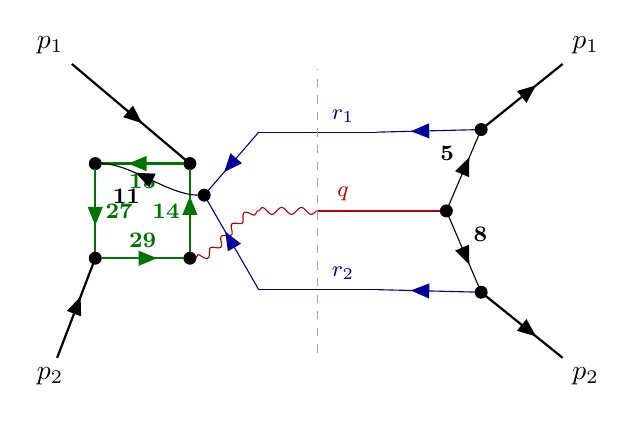
\begin{tikzpicture}
\begin{feynman}
\vertex (Lp1) at (-3.400,2.100) {$p_1$};
\vertex (Lp2) at (-3.400,-2.100) {$p_2$};
\vertex (Lcr1) at (-0.750,1.000);
\vertex (Lcr2) at (-0.750,-1.000);
\vertex (Lcq) at (-0.750,0.000);
\vertex (Mq) at (0,0.000);
\vertex[dot] (Lv0) at (-1.624,-0.601) {};
\vertex[dot] (Lv1) at (-1.624,0.601) {};
\vertex[dot] (Lv2) at (-2.826,0.601) {};
\vertex[dot] (Lv3) at (-2.826,-0.601) {};
\vertex[dot] (Lt11) at (-1.442,0.200) {};
\vertex (Rp1) at (3.400,2.100) {$p_1$};
\vertex (Rp2) at (3.400,-2.100) {$p_2$};
\vertex (Rcr1) at (0.750,1.000);
\vertex (Rcr2) at (0.750,-1.000);
\vertex (Rcq) at (0.750,0.000);
\vertex[dot] (R5) at (2.075,1.033) {};
\vertex[dot] (Rroot) at (1.633,0.000) {};
\vertex[dot] (R8) at (2.075,-1.033) {};
\diagram* {
(Lv0) -- [plain, thick, green!45!black, with arrow=0.55, edge label={\footnotesize\bfseries 14}] (Lv1),
(Lv1) -- [plain, thick, green!45!black, with arrow=0.55, edge label={\footnotesize\bfseries 15}] (Lv2),
(Lv2) -- [plain, thick, green!45!black, with arrow=0.55, edge label={\footnotesize\bfseries 27}] (Lv3),
(Lv3) -- [plain, thick, green!45!black, with arrow=0.55, edge label={\footnotesize\bfseries 29}] (Lv0),
(Lcq) -- [boson, red!70!black, out=180, in=0, looseness=0.75] (Lv0),
(Lp1) -- [plain, thick, with arrow=0.55] (Lv1),
(Lt11) -- [plain, out=180, in=0, looseness=0.75, with arrow=0.55, edge label={\footnotesize\bfseries 11}] (Lv2),
(Lcr1) -- [plain, blue!60!black, with arrow=0.55] (Lt11),
(Lcr2) -- [plain, blue!60!black, with arrow=0.55] (Lt11),
(Lp2) -- [plain, thick, with arrow=0.55] (Lv3),
(Rroot) -- [plain, with arrow=0.55, edge label={\footnotesize\bfseries 5}] (R5),
(Rroot) -- [plain, with arrow=0.55, edge label={\footnotesize\bfseries 8}] (R8),
(R5) -- [plain, thick, with arrow=0.55] (Rp1),
(R8) -- [plain, thick, with arrow=0.55] (Rp2),
(R5) -- [plain, blue!60!black, with arrow=0.55] (Rcr1),
(R8) -- [plain, blue!60!black, with arrow=0.55] (Rcr2),
(Rroot) -- [plain, red!70!black, double, double distance=1.2pt, thick] (Rcq),
(Rcr1) -- [plain, blue!60!black] (Lcr1),
(Rcr2) -- [plain, blue!60!black] (Lcr2),
(Rcq) -- [plain, red!70!black, double, double distance=1.2pt, thick] (Mq) -- [boson, red!70!black] (Lcq),
};
\end{feynman}
\draw[dashed, gray!70] (0,-1.80) -- (0,1.80);
\node[font=\footnotesize, blue!60!black, above] at (0.32,1.00) {$r_1$};
\node[font=\footnotesize, blue!60!black, above] at (0.32,-1.00) {$r_2$};
\node[font=\footnotesize, red!70!black, above] at (0.32,0.00) {$q$};
\end{tikzpicture}}\\[2mm]\textbf{topo3} (RR family 8, pentagon q-p1-r1-r2-p2), sector with 7 of 8 lines\\[2pt]{\footnotesize\begin{tabular}{@{}r@{\ \ }l@{\ \ }l@{}}\textbf{14} & $(k_1)^2$ & loop\\
\textbf{15} & $(k_1+p_1)^2$ & loop\\
\textbf{27} & $(k_1+p_1+r_1+r_2)^2$ & loop\\
\textbf{29} & $(k_1+p_1+p_2+r_1+r_2)^2$ & loop\\
\textbf{11} & $(r_1+r_2)^2$ & amplitude (tree on the loop)\\
\textbf{5} & $(p_1+r_1)^2$ & conjugate\\
\textbf{8} & $(p_2+r_2)^2$ & conjugate\\\end{tabular}}\\[2pt]{\scriptsize pinched: 19 = $(k_1+p_1+r_1)^2$}\end{minipage}\hfill%
\begin{minipage}[t]{0.48\textwidth}\centering\resizebox{0.9\linewidth}{!}{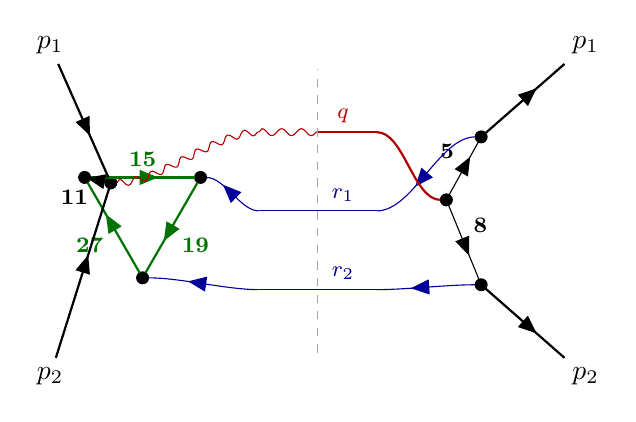
\begin{tikzpicture}
\begin{feynman}
\vertex (Lp1) at (-3.400,2.100) {$p_1$};
\vertex (Lp2) at (-3.400,-2.100) {$p_2$};
\vertex (Lcr1) at (-0.750,0.000);
\vertex (Lcr2) at (-0.750,-1.000);
\vertex (Lcq) at (-0.750,1.000);
\vertex (Mq) at (0,1.000);
\vertex[dot] (Lv0) at (-2.961,0.425) {};
\vertex[dot] (Lv1) at (-1.489,0.425) {};
\vertex[dot] (Lv2) at (-2.225,-0.850) {};
\vertex[dot] (Lt11) at (-2.628,0.356) {};
\vertex (Rp1) at (3.400,2.100) {$p_1$};
\vertex (Rp2) at (3.400,-2.100) {$p_2$};
\vertex (Rcr1) at (0.750,0.000);
\vertex (Rcr2) at (0.750,-1.000);
\vertex (Rcq) at (0.750,1.000);
\vertex[dot] (R5) at (2.075,0.940) {};
\vertex[dot] (Rroot) at (1.633,0.140) {};
\vertex[dot] (R8) at (2.075,-0.938) {};
\diagram* {
(Lv0) -- [plain, thick, green!45!black, with arrow=0.55, edge label={\footnotesize\bfseries 15}] (Lv1),
(Lv1) -- [plain, thick, green!45!black, with arrow=0.55, edge label={\footnotesize\bfseries 19}] (Lv2),
(Lv2) -- [plain, thick, green!45!black, with arrow=0.55, edge label={\footnotesize\bfseries 27}] (Lv0),
(Lt11) -- [plain, with arrow=0.55, edge label={\footnotesize\bfseries 11}] (Lv0),
(Lp2) -- [plain, thick, with arrow=0.55] (Lt11),
(Lcq) -- [boson, red!70!black, out=180, in=0, looseness=0.75] (Lt11),
(Lp1) -- [plain, thick, with arrow=0.55] (Lt11),
(Lcr1) -- [plain, blue!60!black, out=180, in=0, looseness=0.75, with arrow=0.55] (Lv1),
(Lcr2) -- [plain, blue!60!black, out=180, in=0, looseness=0.75, with arrow=0.55] (Lv2),
(Rroot) -- [plain, with arrow=0.55, edge label={\footnotesize\bfseries 5}] (R5),
(Rroot) -- [plain, with arrow=0.55, edge label={\footnotesize\bfseries 8}] (R8),
(R5) -- [plain, thick, with arrow=0.55] (Rp1),
(R8) -- [plain, thick, with arrow=0.55] (Rp2),
(R5) -- [plain, blue!60!black, out=180, in=0, looseness=0.75, with arrow=0.55] (Rcr1),
(R8) -- [plain, blue!60!black, out=180, in=0, looseness=0.75, with arrow=0.55] (Rcr2),
(Rroot) -- [plain, red!70!black, double, double distance=1.2pt, thick, out=180, in=0, looseness=0.75] (Rcq),
(Rcr1) -- [plain, blue!60!black] (Lcr1),
(Rcr2) -- [plain, blue!60!black] (Lcr2),
(Rcq) -- [plain, red!70!black, double, double distance=1.2pt, thick] (Mq) -- [boson, red!70!black] (Lcq),
};
\end{feynman}
\draw[dashed, gray!70] (0,-1.80) -- (0,1.80);
\node[font=\footnotesize, blue!60!black, above] at (0.32,0.00) {$r_1$};
\node[font=\footnotesize, blue!60!black, above] at (0.32,-1.00) {$r_2$};
\node[font=\footnotesize, red!70!black, above] at (0.32,1.00) {$q$};
\end{tikzpicture}}\\[2mm]\textbf{topo3} (RR family 8, pentagon q-p1-r1-r2-p2), sector with 6 of 8 lines\\[2pt]{\footnotesize\begin{tabular}{@{}r@{\ \ }l@{\ \ }l@{}}\textbf{15} & $(k_1+p_1)^2$ & loop\\
\textbf{19} & $(k_1+p_1+r_1)^2$ & loop\\
\textbf{27} & $(k_1+p_1+r_1+r_2)^2$ & loop\\
\textbf{11} & $(r_1+r_2)^2$ & amplitude (tree on the loop)\\
\textbf{5} & $(p_1+r_1)^2$ & conjugate\\
\textbf{8} & $(p_2+r_2)^2$ & conjugate\\\end{tabular}}\\[2pt]{\scriptsize pinched: 14 = $(k_1)^2$, 29 = $(k_1+p_1+p_2+r_1+r_2)^2$}\end{minipage}

\bigskip

\begin{minipage}[t]{0.48\textwidth}\centering\resizebox{0.9\linewidth}{!}{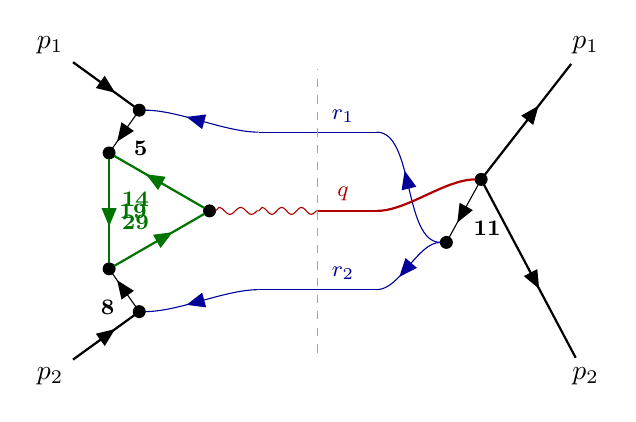
\begin{tikzpicture}
\begin{feynman}
\vertex (Lp1) at (-3.400,2.100) {$p_1$};
\vertex (Lp2) at (-3.400,-2.100) {$p_2$};
\vertex (Lcr1) at (-0.750,1.000);
\vertex (Lcr2) at (-0.750,-1.000);
\vertex (Lcq) at (-0.750,0.000);
\vertex (Mq) at (0,0.000);
\vertex[dot] (Lv0) at (-1.375,0.000) {};
\vertex[dot] (Lv1) at (-2.650,0.736) {};
\vertex[dot] (Lv2) at (-2.650,-0.736) {};
\vertex[dot] (Lt5) at (-2.267,1.279) {};
\vertex[dot] (Lt8) at (-2.267,-1.279) {};
\vertex (Rp1) at (3.400,2.100) {$p_1$};
\vertex (Rp2) at (3.400,-2.100) {$p_2$};
\vertex (Rcr1) at (0.750,1.000);
\vertex (Rcr2) at (0.750,-1.000);
\vertex (Rcq) at (0.750,0.000);
\vertex[dot] (R11) at (1.633,-0.400) {};
\vertex[dot] (Rroot) at (2.075,0.400) {};
\diagram* {
(Lv0) -- [plain, thick, green!45!black, with arrow=0.55, edge label={\footnotesize\bfseries 14}] (Lv1),
(Lv1) -- [plain, thick, green!45!black, with arrow=0.55, edge label={\footnotesize\bfseries 19}] (Lv2),
(Lv2) -- [plain, thick, green!45!black, with arrow=0.55, edge label={\footnotesize\bfseries 29}] (Lv0),
(Lcq) -- [boson, red!70!black] (Lv0),
(Lt5) -- [plain, with arrow=0.55, edge label={\footnotesize\bfseries 5}] (Lv1),
(Lcr1) -- [plain, blue!60!black, out=180, in=0, looseness=0.75, with arrow=0.55] (Lt5),
(Lp1) -- [plain, thick, with arrow=0.55] (Lt5),
(Lt8) -- [plain, with arrow=0.55, edge label={\footnotesize\bfseries 8}] (Lv2),
(Lp2) -- [plain, thick, with arrow=0.55] (Lt8),
(Lcr2) -- [plain, blue!60!black, out=180, in=0, looseness=0.75, with arrow=0.55] (Lt8),
(Rroot) -- [plain, with arrow=0.55, edge label={\footnotesize\bfseries 11}] (R11),
(Rroot) -- [plain, thick, with arrow=0.55] (Rp1),
(Rroot) -- [plain, thick, with arrow=0.55] (Rp2),
(R11) -- [plain, blue!60!black, out=180, in=0, looseness=0.75, with arrow=0.55] (Rcr1),
(R11) -- [plain, blue!60!black, out=180, in=0, looseness=0.75, with arrow=0.55] (Rcr2),
(Rroot) -- [plain, red!70!black, double, double distance=1.2pt, thick, out=180, in=0, looseness=0.75] (Rcq),
(Rcr1) -- [plain, blue!60!black] (Lcr1),
(Rcr2) -- [plain, blue!60!black] (Lcr2),
(Rcq) -- [plain, red!70!black, double, double distance=1.2pt, thick] (Mq) -- [boson, red!70!black] (Lcq),
};
\end{feynman}
\draw[dashed, gray!70] (0,-1.80) -- (0,1.80);
\node[font=\footnotesize, blue!60!black, above] at (0.32,1.00) {$r_1$};
\node[font=\footnotesize, blue!60!black, above] at (0.32,-1.00) {$r_2$};
\node[font=\footnotesize, red!70!black, above] at (0.32,0.00) {$q$};
\end{tikzpicture}}\\[2mm]\textbf{topo3} (RR family 8, pentagon q-p1-r1-r2-p2), sector with 6 of 8 lines\\[2pt]{\footnotesize\begin{tabular}{@{}r@{\ \ }l@{\ \ }l@{}}\textbf{14} & $(k_1)^2$ & loop\\
\textbf{19} & $(k_1+p_1+r_1)^2$ & loop\\
\textbf{29} & $(k_1+p_1+p_2+r_1+r_2)^2$ & loop\\
\textbf{5} & $(p_1+r_1)^2$ & amplitude (tree on the loop)\\
\textbf{8} & $(p_2+r_2)^2$ & amplitude (tree on the loop)\\
\textbf{11} & $(r_1+r_2)^2$ & conjugate\\\end{tabular}}\\[2pt]{\scriptsize pinched: 15 = $(k_1+p_1)^2$, 27 = $(k_1+p_1+r_1+r_2)^2$}\end{minipage}\hfill%
\begin{minipage}[t]{0.48\textwidth}\centering\resizebox{0.9\linewidth}{!}{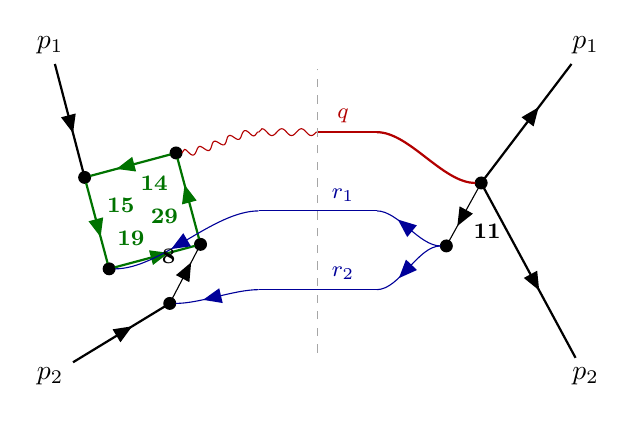
\begin{tikzpicture}
\begin{feynman}
\vertex (Lp1) at (-3.400,2.100) {$p_1$};
\vertex (Lp2) at (-3.400,-2.100) {$p_2$};
\vertex (Lcr1) at (-0.750,0.000);
\vertex (Lcr2) at (-0.750,-1.000);
\vertex (Lcq) at (-0.750,1.000);
\vertex (Mq) at (0,1.000);
\vertex[dot] (Lv0) at (-1.800,0.736) {};
\vertex[dot] (Lv1) at (-2.961,0.425) {};
\vertex[dot] (Lv2) at (-2.650,-0.736) {};
\vertex[dot] (Lv3) at (-1.489,-0.425) {};
\vertex[dot] (Lt8) at (-1.880,-1.175) {};
\vertex (Rp1) at (3.400,2.100) {$p_1$};
\vertex (Rp2) at (3.400,-2.100) {$p_2$};
\vertex (Rcr1) at (0.750,0.000);
\vertex (Rcr2) at (0.750,-1.000);
\vertex (Rcq) at (0.750,1.000);
\vertex[dot] (R11) at (1.633,-0.445) {};
\vertex[dot] (Rroot) at (2.075,0.355) {};
\diagram* {
(Lv0) -- [plain, thick, green!45!black, with arrow=0.55, edge label={\footnotesize\bfseries 14}] (Lv1),
(Lv1) -- [plain, thick, green!45!black, with arrow=0.55, edge label={\footnotesize\bfseries 15}] (Lv2),
(Lv2) -- [plain, thick, green!45!black, with arrow=0.55, edge label={\footnotesize\bfseries 19}] (Lv3),
(Lv3) -- [plain, thick, green!45!black, with arrow=0.55, edge label={\footnotesize\bfseries 29}] (Lv0),
(Lcq) -- [boson, red!70!black, out=180, in=0, looseness=0.75] (Lv0),
(Lp1) -- [plain, thick, with arrow=0.55] (Lv1),
(Lcr1) -- [plain, blue!60!black, out=180, in=0, looseness=0.75, with arrow=0.55] (Lv2),
(Lt8) -- [plain, with arrow=0.55, edge label={\footnotesize\bfseries 8}] (Lv3),
(Lp2) -- [plain, thick, with arrow=0.55] (Lt8),
(Lcr2) -- [plain, blue!60!black, out=180, in=0, looseness=0.75, with arrow=0.55] (Lt8),
(Rroot) -- [plain, with arrow=0.55, edge label={\footnotesize\bfseries 11}] (R11),
(Rroot) -- [plain, thick, with arrow=0.55] (Rp1),
(Rroot) -- [plain, thick, with arrow=0.55] (Rp2),
(R11) -- [plain, blue!60!black, out=180, in=0, looseness=0.75, with arrow=0.55] (Rcr1),
(R11) -- [plain, blue!60!black, out=180, in=0, looseness=0.75, with arrow=0.55] (Rcr2),
(Rroot) -- [plain, red!70!black, double, double distance=1.2pt, thick, out=180, in=0, looseness=0.75] (Rcq),
(Rcr1) -- [plain, blue!60!black] (Lcr1),
(Rcr2) -- [plain, blue!60!black] (Lcr2),
(Rcq) -- [plain, red!70!black, double, double distance=1.2pt, thick] (Mq) -- [boson, red!70!black] (Lcq),
};
\end{feynman}
\draw[dashed, gray!70] (0,-1.80) -- (0,1.80);
\node[font=\footnotesize, blue!60!black, above] at (0.32,0.00) {$r_1$};
\node[font=\footnotesize, blue!60!black, above] at (0.32,-1.00) {$r_2$};
\node[font=\footnotesize, red!70!black, above] at (0.32,1.00) {$q$};
\end{tikzpicture}}\\[2mm]\textbf{topo3} (RR family 8, pentagon q-p1-r1-r2-p2), sector with 6 of 8 lines\\[2pt]{\footnotesize\begin{tabular}{@{}r@{\ \ }l@{\ \ }l@{}}\textbf{14} & $(k_1)^2$ & loop\\
\textbf{15} & $(k_1+p_1)^2$ & loop\\
\textbf{19} & $(k_1+p_1+r_1)^2$ & loop\\
\textbf{29} & $(k_1+p_1+p_2+r_1+r_2)^2$ & loop\\
\textbf{8} & $(p_2+r_2)^2$ & amplitude (tree on the loop)\\
\textbf{11} & $(r_1+r_2)^2$ & conjugate\\\end{tabular}}\\[2pt]{\scriptsize pinched: 5 = $(p_1+r_1)^2$, 27 = $(k_1+p_1+r_1+r_2)^2$}\end{minipage}

\bigskip

\begin{minipage}[t]{0.48\textwidth}\centering\resizebox{0.9\linewidth}{!}{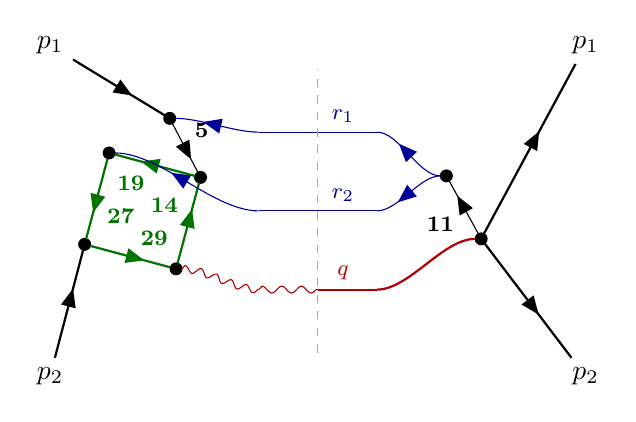
\begin{tikzpicture}
\begin{feynman}
\vertex (Lp1) at (-3.400,2.100) {$p_1$};
\vertex (Lp2) at (-3.400,-2.100) {$p_2$};
\vertex (Lcr1) at (-0.750,1.000);
\vertex (Lcr2) at (-0.750,0.000);
\vertex (Lcq) at (-0.750,-1.000);
\vertex (Mq) at (0,-1.000);
\vertex[dot] (Lv0) at (-1.800,-0.736) {};
\vertex[dot] (Lv1) at (-1.489,0.425) {};
\vertex[dot] (Lv2) at (-2.650,0.736) {};
\vertex[dot] (Lv3) at (-2.961,-0.425) {};
\vertex[dot] (Lt5) at (-1.880,1.175) {};
\vertex (Rp1) at (3.400,2.100) {$p_1$};
\vertex (Rp2) at (3.400,-2.100) {$p_2$};
\vertex (Rcr1) at (0.750,1.000);
\vertex (Rcr2) at (0.750,0.000);
\vertex (Rcq) at (0.750,-1.000);
\vertex[dot] (R11) at (1.633,0.445) {};
\vertex[dot] (Rroot) at (2.075,-0.355) {};
\diagram* {
(Lv0) -- [plain, thick, green!45!black, with arrow=0.55, edge label={\footnotesize\bfseries 14}] (Lv1),
(Lv1) -- [plain, thick, green!45!black, with arrow=0.55, edge label={\footnotesize\bfseries 19}] (Lv2),
(Lv2) -- [plain, thick, green!45!black, with arrow=0.55, edge label={\footnotesize\bfseries 27}] (Lv3),
(Lv3) -- [plain, thick, green!45!black, with arrow=0.55, edge label={\footnotesize\bfseries 29}] (Lv0),
(Lcq) -- [boson, red!70!black, out=180, in=0, looseness=0.75] (Lv0),
(Lt5) -- [plain, with arrow=0.55, edge label={\footnotesize\bfseries 5}] (Lv1),
(Lcr1) -- [plain, blue!60!black, out=180, in=0, looseness=0.75, with arrow=0.55] (Lt5),
(Lp1) -- [plain, thick, with arrow=0.55] (Lt5),
(Lcr2) -- [plain, blue!60!black, out=180, in=0, looseness=0.75, with arrow=0.55] (Lv2),
(Lp2) -- [plain, thick, with arrow=0.55] (Lv3),
(Rroot) -- [plain, with arrow=0.55, edge label={\footnotesize\bfseries 11}] (R11),
(Rroot) -- [plain, thick, with arrow=0.55] (Rp1),
(Rroot) -- [plain, thick, with arrow=0.55] (Rp2),
(R11) -- [plain, blue!60!black, out=180, in=0, looseness=0.75, with arrow=0.55] (Rcr1),
(R11) -- [plain, blue!60!black, out=180, in=0, looseness=0.75, with arrow=0.55] (Rcr2),
(Rroot) -- [plain, red!70!black, double, double distance=1.2pt, thick, out=180, in=0, looseness=0.75] (Rcq),
(Rcr1) -- [plain, blue!60!black] (Lcr1),
(Rcr2) -- [plain, blue!60!black] (Lcr2),
(Rcq) -- [plain, red!70!black, double, double distance=1.2pt, thick] (Mq) -- [boson, red!70!black] (Lcq),
};
\end{feynman}
\draw[dashed, gray!70] (0,-1.80) -- (0,1.80);
\node[font=\footnotesize, blue!60!black, above] at (0.32,1.00) {$r_1$};
\node[font=\footnotesize, blue!60!black, above] at (0.32,0.00) {$r_2$};
\node[font=\footnotesize, red!70!black, above] at (0.32,-1.00) {$q$};
\end{tikzpicture}}\\[2mm]\textbf{topo3} (RR family 8, pentagon q-p1-r1-r2-p2), sector with 6 of 8 lines\\[2pt]{\footnotesize\begin{tabular}{@{}r@{\ \ }l@{\ \ }l@{}}\textbf{14} & $(k_1)^2$ & loop\\
\textbf{19} & $(k_1+p_1+r_1)^2$ & loop\\
\textbf{27} & $(k_1+p_1+r_1+r_2)^2$ & loop\\
\textbf{29} & $(k_1+p_1+p_2+r_1+r_2)^2$ & loop\\
\textbf{5} & $(p_1+r_1)^2$ & amplitude (tree on the loop)\\
\textbf{11} & $(r_1+r_2)^2$ & conjugate\\\end{tabular}}\\[2pt]{\scriptsize pinched: 8 = $(p_2+r_2)^2$, 15 = $(k_1+p_1)^2$}\end{minipage}\hfill%
\begin{minipage}[t]{0.48\textwidth}\centering\resizebox{0.9\linewidth}{!}{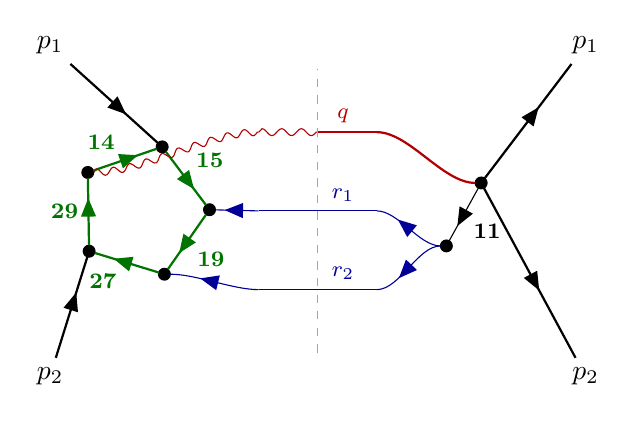
\begin{tikzpicture}
\begin{feynman}
\vertex (Lp1) at (-3.400,2.100) {$p_1$};
\vertex (Lp2) at (-3.400,-2.100) {$p_2$};
\vertex (Lcr1) at (-0.750,0.000);
\vertex (Lcr2) at (-0.750,-1.000);
\vertex (Lcq) at (-0.750,1.000);
\vertex (Mq) at (0,1.000);
\vertex[dot] (Lv0) at (-2.921,0.488) {};
\vertex[dot] (Lv1) at (-1.976,0.813) {};
\vertex[dot] (Lv2) at (-1.375,0.015) {};
\vertex[dot] (Lv3) at (-1.948,-0.804) {};
\vertex[dot] (Lv4) at (-2.904,-0.512) {};
\vertex (Rp1) at (3.400,2.100) {$p_1$};
\vertex (Rp2) at (3.400,-2.100) {$p_2$};
\vertex (Rcr1) at (0.750,0.000);
\vertex (Rcr2) at (0.750,-1.000);
\vertex (Rcq) at (0.750,1.000);
\vertex[dot] (R11) at (1.633,-0.445) {};
\vertex[dot] (Rroot) at (2.075,0.355) {};
\diagram* {
(Lv0) -- [plain, thick, green!45!black, with arrow=0.55, edge label={\footnotesize\bfseries 14}] (Lv1),
(Lv1) -- [plain, thick, green!45!black, with arrow=0.55, edge label={\footnotesize\bfseries 15}] (Lv2),
(Lv2) -- [plain, thick, green!45!black, with arrow=0.55, edge label={\footnotesize\bfseries 19}] (Lv3),
(Lv3) -- [plain, thick, green!45!black, with arrow=0.55, edge label={\footnotesize\bfseries 27}] (Lv4),
(Lv4) -- [plain, thick, green!45!black, with arrow=0.55, edge label={\footnotesize\bfseries 29}] (Lv0),
(Lcq) -- [boson, red!70!black, out=180, in=0, looseness=0.75] (Lv0),
(Lp1) -- [plain, thick, with arrow=0.55] (Lv1),
(Lcr1) -- [plain, blue!60!black, with arrow=0.55] (Lv2),
(Lcr2) -- [plain, blue!60!black, out=180, in=0, looseness=0.75, with arrow=0.55] (Lv3),
(Lp2) -- [plain, thick, with arrow=0.55] (Lv4),
(Rroot) -- [plain, with arrow=0.55, edge label={\footnotesize\bfseries 11}] (R11),
(Rroot) -- [plain, thick, with arrow=0.55] (Rp1),
(Rroot) -- [plain, thick, with arrow=0.55] (Rp2),
(R11) -- [plain, blue!60!black, out=180, in=0, looseness=0.75, with arrow=0.55] (Rcr1),
(R11) -- [plain, blue!60!black, out=180, in=0, looseness=0.75, with arrow=0.55] (Rcr2),
(Rroot) -- [plain, red!70!black, double, double distance=1.2pt, thick, out=180, in=0, looseness=0.75] (Rcq),
(Rcr1) -- [plain, blue!60!black] (Lcr1),
(Rcr2) -- [plain, blue!60!black] (Lcr2),
(Rcq) -- [plain, red!70!black, double, double distance=1.2pt, thick] (Mq) -- [boson, red!70!black] (Lcq),
};
\end{feynman}
\draw[dashed, gray!70] (0,-1.80) -- (0,1.80);
\node[font=\footnotesize, blue!60!black, above] at (0.32,0.00) {$r_1$};
\node[font=\footnotesize, blue!60!black, above] at (0.32,-1.00) {$r_2$};
\node[font=\footnotesize, red!70!black, above] at (0.32,1.00) {$q$};
\end{tikzpicture}}\\[2mm]\textbf{topo3} (RR family 8, pentagon q-p1-r1-r2-p2), sector with 6 of 8 lines\\[2pt]{\footnotesize\begin{tabular}{@{}r@{\ \ }l@{\ \ }l@{}}\textbf{14} & $(k_1)^2$ & loop\\
\textbf{15} & $(k_1+p_1)^2$ & loop\\
\textbf{19} & $(k_1+p_1+r_1)^2$ & loop\\
\textbf{27} & $(k_1+p_1+r_1+r_2)^2$ & loop\\
\textbf{29} & $(k_1+p_1+p_2+r_1+r_2)^2$ & loop\\
\textbf{11} & $(r_1+r_2)^2$ & conjugate\\\end{tabular}}\\[2pt]{\scriptsize pinched: 5 = $(p_1+r_1)^2$, 8 = $(p_2+r_2)^2$}\end{minipage}

\bigskip

\begin{minipage}[t]{0.48\textwidth}\centering\resizebox{0.9\linewidth}{!}{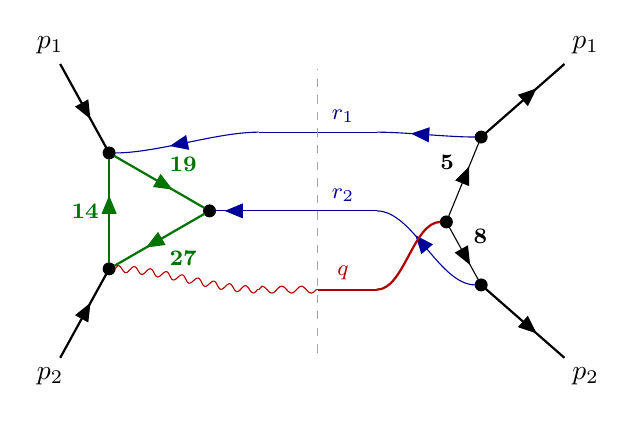
\begin{tikzpicture}
\begin{feynman}
\vertex (Lp1) at (-3.400,2.100) {$p_1$};
\vertex (Lp2) at (-3.400,-2.100) {$p_2$};
\vertex (Lcr1) at (-0.750,1.000);
\vertex (Lcr2) at (-0.750,0.000);
\vertex (Lcq) at (-0.750,-1.000);
\vertex (Mq) at (0,-1.000);
\vertex[dot] (Lv0) at (-2.650,-0.736) {};
\vertex[dot] (Lv1) at (-2.650,0.736) {};
\vertex[dot] (Lv2) at (-1.375,0.000) {};
\vertex (Rp1) at (3.400,2.100) {$p_1$};
\vertex (Rp2) at (3.400,-2.100) {$p_2$};
\vertex (Rcr1) at (0.750,1.000);
\vertex (Rcr2) at (0.750,0.000);
\vertex (Rcq) at (0.750,-1.000);
\vertex[dot] (R5) at (2.075,0.938) {};
\vertex[dot] (Rroot) at (1.633,-0.140) {};
\vertex[dot] (R8) at (2.075,-0.940) {};
\diagram* {
(Lv0) -- [plain, thick, green!45!black, with arrow=0.55, edge label={\footnotesize\bfseries 14}] (Lv1),
(Lv1) -- [plain, thick, green!45!black, with arrow=0.55, edge label={\footnotesize\bfseries 19}] (Lv2),
(Lv2) -- [plain, thick, green!45!black, with arrow=0.55, edge label={\footnotesize\bfseries 27}] (Lv0),
(Lp2) -- [plain, thick, with arrow=0.55] (Lv0),
(Lcq) -- [boson, red!70!black, out=180, in=0, looseness=0.75] (Lv0),
(Lcr1) -- [plain, blue!60!black, out=180, in=0, looseness=0.75, with arrow=0.55] (Lv1),
(Lp1) -- [plain, thick, with arrow=0.55] (Lv1),
(Lcr2) -- [plain, blue!60!black, with arrow=0.55] (Lv2),
(Rroot) -- [plain, with arrow=0.55, edge label={\footnotesize\bfseries 5}] (R5),
(Rroot) -- [plain, with arrow=0.55, edge label={\footnotesize\bfseries 8}] (R8),
(R5) -- [plain, thick, with arrow=0.55] (Rp1),
(R8) -- [plain, thick, with arrow=0.55] (Rp2),
(R5) -- [plain, blue!60!black, out=180, in=0, looseness=0.75, with arrow=0.55] (Rcr1),
(R8) -- [plain, blue!60!black, out=180, in=0, looseness=0.75, with arrow=0.55] (Rcr2),
(Rroot) -- [plain, red!70!black, double, double distance=1.2pt, thick, out=180, in=0, looseness=0.75] (Rcq),
(Rcr1) -- [plain, blue!60!black] (Lcr1),
(Rcr2) -- [plain, blue!60!black] (Lcr2),
(Rcq) -- [plain, red!70!black, double, double distance=1.2pt, thick] (Mq) -- [boson, red!70!black] (Lcq),
};
\end{feynman}
\draw[dashed, gray!70] (0,-1.80) -- (0,1.80);
\node[font=\footnotesize, blue!60!black, above] at (0.32,1.00) {$r_1$};
\node[font=\footnotesize, blue!60!black, above] at (0.32,0.00) {$r_2$};
\node[font=\footnotesize, red!70!black, above] at (0.32,-1.00) {$q$};
\end{tikzpicture}}\\[2mm]\textbf{topo3} (RR family 8, pentagon q-p1-r1-r2-p2), sector with 5 of 8 lines\\[2pt]{\footnotesize\begin{tabular}{@{}r@{\ \ }l@{\ \ }l@{}}\textbf{14} & $(k_1)^2$ & loop\\
\textbf{19} & $(k_1+p_1+r_1)^2$ & loop\\
\textbf{27} & $(k_1+p_1+r_1+r_2)^2$ & loop\\
\textbf{5} & $(p_1+r_1)^2$ & conjugate\\
\textbf{8} & $(p_2+r_2)^2$ & conjugate\\\end{tabular}}\\[2pt]{\scriptsize pinched: 11 = $(r_1+r_2)^2$, 15 = $(k_1+p_1)^2$, 29 = $(k_1+p_1+p_2+r_1+r_2)^2$}\end{minipage}\hfill%
\begin{minipage}[t]{0.48\textwidth}\centering\resizebox{0.9\linewidth}{!}{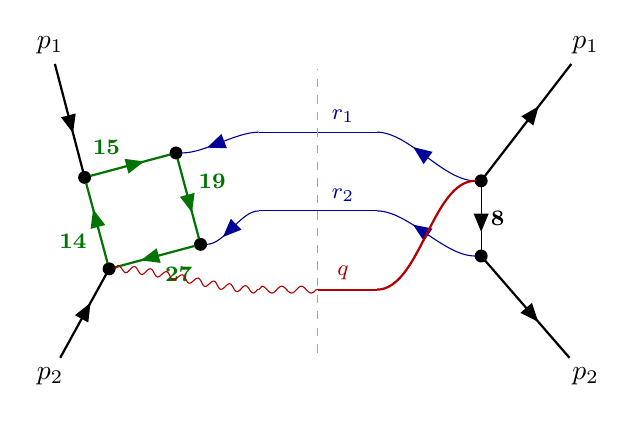
\begin{tikzpicture}
\begin{feynman}
\vertex (Lp1) at (-3.400,2.100) {$p_1$};
\vertex (Lp2) at (-3.400,-2.100) {$p_2$};
\vertex (Lcr1) at (-0.750,1.000);
\vertex (Lcr2) at (-0.750,0.000);
\vertex (Lcq) at (-0.750,-1.000);
\vertex (Mq) at (0,-1.000);
\vertex[dot] (Lv0) at (-2.650,-0.736) {};
\vertex[dot] (Lv1) at (-2.961,0.425) {};
\vertex[dot] (Lv2) at (-1.800,0.736) {};
\vertex[dot] (Lv3) at (-1.489,-0.425) {};
\vertex (Rp1) at (3.400,2.100) {$p_1$};
\vertex (Rp2) at (3.400,-2.100) {$p_2$};
\vertex (Rcr1) at (0.750,1.000);
\vertex (Rcr2) at (0.750,0.000);
\vertex (Rcq) at (0.750,-1.000);
\vertex[dot] (R8) at (2.075,-0.573) {};
\vertex[dot] (Rroot) at (2.075,0.382) {};
\diagram* {
(Lv0) -- [plain, thick, green!45!black, with arrow=0.55, edge label={\footnotesize\bfseries 14}] (Lv1),
(Lv1) -- [plain, thick, green!45!black, with arrow=0.55, edge label={\footnotesize\bfseries 15}] (Lv2),
(Lv2) -- [plain, thick, green!45!black, with arrow=0.55, edge label={\footnotesize\bfseries 19}] (Lv3),
(Lv3) -- [plain, thick, green!45!black, with arrow=0.55, edge label={\footnotesize\bfseries 27}] (Lv0),
(Lp2) -- [plain, thick, with arrow=0.55] (Lv0),
(Lcq) -- [boson, red!70!black, out=180, in=0, looseness=0.75] (Lv0),
(Lp1) -- [plain, thick, with arrow=0.55] (Lv1),
(Lcr1) -- [plain, blue!60!black, out=180, in=0, looseness=0.75, with arrow=0.55] (Lv2),
(Lcr2) -- [plain, blue!60!black, out=180, in=0, looseness=0.75, with arrow=0.55] (Lv3),
(Rroot) -- [plain, with arrow=0.55, edge label={\footnotesize\bfseries 8}] (R8),
(Rroot) -- [plain, thick, with arrow=0.55] (Rp1),
(R8) -- [plain, thick, with arrow=0.55] (Rp2),
(Rroot) -- [plain, blue!60!black, out=180, in=0, looseness=0.75, with arrow=0.55] (Rcr1),
(R8) -- [plain, blue!60!black, out=180, in=0, looseness=0.75, with arrow=0.55] (Rcr2),
(Rroot) -- [plain, red!70!black, double, double distance=1.2pt, thick, out=180, in=0, looseness=0.75] (Rcq),
(Rcr1) -- [plain, blue!60!black] (Lcr1),
(Rcr2) -- [plain, blue!60!black] (Lcr2),
(Rcq) -- [plain, red!70!black, double, double distance=1.2pt, thick] (Mq) -- [boson, red!70!black] (Lcq),
};
\end{feynman}
\draw[dashed, gray!70] (0,-1.80) -- (0,1.80);
\node[font=\footnotesize, blue!60!black, above] at (0.32,1.00) {$r_1$};
\node[font=\footnotesize, blue!60!black, above] at (0.32,0.00) {$r_2$};
\node[font=\footnotesize, red!70!black, above] at (0.32,-1.00) {$q$};
\end{tikzpicture}}\\[2mm]\textbf{topo3} (RR family 8, pentagon q-p1-r1-r2-p2), sector with 5 of 8 lines\\[2pt]{\footnotesize\begin{tabular}{@{}r@{\ \ }l@{\ \ }l@{}}\textbf{14} & $(k_1)^2$ & loop\\
\textbf{15} & $(k_1+p_1)^2$ & loop\\
\textbf{19} & $(k_1+p_1+r_1)^2$ & loop\\
\textbf{27} & $(k_1+p_1+r_1+r_2)^2$ & loop\\
\textbf{8} & $(p_2+r_2)^2$ & conjugate\\\end{tabular}}\\[2pt]{\scriptsize pinched: 5 = $(p_1+r_1)^2$, 11 = $(r_1+r_2)^2$, 29 = $(k_1+p_1+p_2+r_1+r_2)^2$}\end{minipage}

\bigskip

\begin{minipage}[t]{0.48\textwidth}\centering\resizebox{0.9\linewidth}{!}{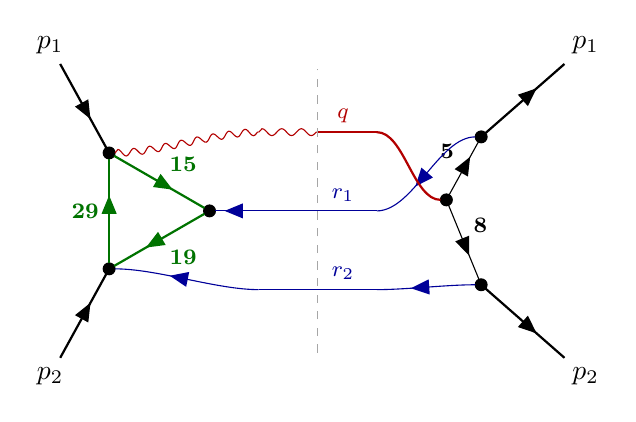
\begin{tikzpicture}
\begin{feynman}
\vertex (Lp1) at (-3.400,2.100) {$p_1$};
\vertex (Lp2) at (-3.400,-2.100) {$p_2$};
\vertex (Lcr1) at (-0.750,0.000);
\vertex (Lcr2) at (-0.750,-1.000);
\vertex (Lcq) at (-0.750,1.000);
\vertex (Mq) at (0,1.000);
\vertex[dot] (Lv0) at (-2.650,0.736) {};
\vertex[dot] (Lv1) at (-1.375,0.000) {};
\vertex[dot] (Lv2) at (-2.650,-0.736) {};
\vertex (Rp1) at (3.400,2.100) {$p_1$};
\vertex (Rp2) at (3.400,-2.100) {$p_2$};
\vertex (Rcr1) at (0.750,0.000);
\vertex (Rcr2) at (0.750,-1.000);
\vertex (Rcq) at (0.750,1.000);
\vertex[dot] (R5) at (2.075,0.940) {};
\vertex[dot] (Rroot) at (1.633,0.140) {};
\vertex[dot] (R8) at (2.075,-0.938) {};
\diagram* {
(Lv0) -- [plain, thick, green!45!black, with arrow=0.55, edge label={\footnotesize\bfseries 15}] (Lv1),
(Lv1) -- [plain, thick, green!45!black, with arrow=0.55, edge label={\footnotesize\bfseries 19}] (Lv2),
(Lv2) -- [plain, thick, green!45!black, with arrow=0.55, edge label={\footnotesize\bfseries 29}] (Lv0),
(Lcq) -- [boson, red!70!black, out=180, in=0, looseness=0.75] (Lv0),
(Lp1) -- [plain, thick, with arrow=0.55] (Lv0),
(Lcr1) -- [plain, blue!60!black, with arrow=0.55] (Lv1),
(Lp2) -- [plain, thick, with arrow=0.55] (Lv2),
(Lcr2) -- [plain, blue!60!black, out=180, in=0, looseness=0.75, with arrow=0.55] (Lv2),
(Rroot) -- [plain, with arrow=0.55, edge label={\footnotesize\bfseries 5}] (R5),
(Rroot) -- [plain, with arrow=0.55, edge label={\footnotesize\bfseries 8}] (R8),
(R5) -- [plain, thick, with arrow=0.55] (Rp1),
(R8) -- [plain, thick, with arrow=0.55] (Rp2),
(R5) -- [plain, blue!60!black, out=180, in=0, looseness=0.75, with arrow=0.55] (Rcr1),
(R8) -- [plain, blue!60!black, out=180, in=0, looseness=0.75, with arrow=0.55] (Rcr2),
(Rroot) -- [plain, red!70!black, double, double distance=1.2pt, thick, out=180, in=0, looseness=0.75] (Rcq),
(Rcr1) -- [plain, blue!60!black] (Lcr1),
(Rcr2) -- [plain, blue!60!black] (Lcr2),
(Rcq) -- [plain, red!70!black, double, double distance=1.2pt, thick] (Mq) -- [boson, red!70!black] (Lcq),
};
\end{feynman}
\draw[dashed, gray!70] (0,-1.80) -- (0,1.80);
\node[font=\footnotesize, blue!60!black, above] at (0.32,0.00) {$r_1$};
\node[font=\footnotesize, blue!60!black, above] at (0.32,-1.00) {$r_2$};
\node[font=\footnotesize, red!70!black, above] at (0.32,1.00) {$q$};
\end{tikzpicture}}\\[2mm]\textbf{topo3} (RR family 8, pentagon q-p1-r1-r2-p2), sector with 5 of 8 lines\\[2pt]{\footnotesize\begin{tabular}{@{}r@{\ \ }l@{\ \ }l@{}}\textbf{15} & $(k_1+p_1)^2$ & loop\\
\textbf{19} & $(k_1+p_1+r_1)^2$ & loop\\
\textbf{29} & $(k_1+p_1+p_2+r_1+r_2)^2$ & loop\\
\textbf{5} & $(p_1+r_1)^2$ & conjugate\\
\textbf{8} & $(p_2+r_2)^2$ & conjugate\\\end{tabular}}\\[2pt]{\scriptsize pinched: 11 = $(r_1+r_2)^2$, 14 = $(k_1)^2$, 27 = $(k_1+p_1+r_1+r_2)^2$}\end{minipage}\hfill%
\begin{minipage}[t]{0.48\textwidth}\centering\resizebox{0.9\linewidth}{!}{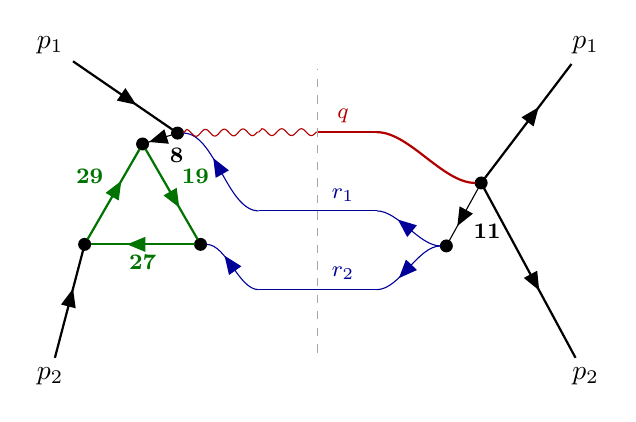
\begin{tikzpicture}
\begin{feynman}
\vertex (Lp1) at (-3.400,2.100) {$p_1$};
\vertex (Lp2) at (-3.400,-2.100) {$p_2$};
\vertex (Lcr1) at (-0.750,0.000);
\vertex (Lcr2) at (-0.750,-1.000);
\vertex (Lcq) at (-0.750,1.000);
\vertex (Mq) at (0,1.000);
\vertex[dot] (Lv0) at (-2.225,0.850) {};
\vertex[dot] (Lv1) at (-1.489,-0.425) {};
\vertex[dot] (Lv2) at (-2.961,-0.425) {};
\vertex[dot] (Lt8) at (-1.781,0.988) {};
\vertex (Rp1) at (3.400,2.100) {$p_1$};
\vertex (Rp2) at (3.400,-2.100) {$p_2$};
\vertex (Rcr1) at (0.750,0.000);
\vertex (Rcr2) at (0.750,-1.000);
\vertex (Rcq) at (0.750,1.000);
\vertex[dot] (R11) at (1.633,-0.445) {};
\vertex[dot] (Rroot) at (2.075,0.355) {};
\diagram* {
(Lv0) -- [plain, thick, green!45!black, with arrow=0.55, edge label={\footnotesize\bfseries 19}] (Lv1),
(Lv1) -- [plain, thick, green!45!black, with arrow=0.55, edge label={\footnotesize\bfseries 27}] (Lv2),
(Lv2) -- [plain, thick, green!45!black, with arrow=0.55, edge label={\footnotesize\bfseries 29}] (Lv0),
(Lt8) -- [plain, with arrow=0.55, edge label={\footnotesize\bfseries 8}] (Lv0),
(Lcr1) -- [plain, blue!60!black, out=180, in=0, looseness=0.75, with arrow=0.55] (Lt8),
(Lcq) -- [boson, red!70!black] (Lt8),
(Lp1) -- [plain, thick, with arrow=0.55] (Lt8),
(Lcr2) -- [plain, blue!60!black, out=180, in=0, looseness=0.75, with arrow=0.55] (Lv1),
(Lp2) -- [plain, thick, with arrow=0.55] (Lv2),
(Rroot) -- [plain, with arrow=0.55, edge label={\footnotesize\bfseries 11}] (R11),
(Rroot) -- [plain, thick, with arrow=0.55] (Rp1),
(Rroot) -- [plain, thick, with arrow=0.55] (Rp2),
(R11) -- [plain, blue!60!black, out=180, in=0, looseness=0.75, with arrow=0.55] (Rcr1),
(R11) -- [plain, blue!60!black, out=180, in=0, looseness=0.75, with arrow=0.55] (Rcr2),
(Rroot) -- [plain, red!70!black, double, double distance=1.2pt, thick, out=180, in=0, looseness=0.75] (Rcq),
(Rcr1) -- [plain, blue!60!black] (Lcr1),
(Rcr2) -- [plain, blue!60!black] (Lcr2),
(Rcq) -- [plain, red!70!black, double, double distance=1.2pt, thick] (Mq) -- [boson, red!70!black] (Lcq),
};
\end{feynman}
\draw[dashed, gray!70] (0,-1.80) -- (0,1.80);
\node[font=\footnotesize, blue!60!black, above] at (0.32,0.00) {$r_1$};
\node[font=\footnotesize, blue!60!black, above] at (0.32,-1.00) {$r_2$};
\node[font=\footnotesize, red!70!black, above] at (0.32,1.00) {$q$};
\end{tikzpicture}}\\[2mm]\textbf{topo3} (RR family 8, pentagon q-p1-r1-r2-p2), sector with 5 of 8 lines\\[2pt]{\footnotesize\begin{tabular}{@{}r@{\ \ }l@{\ \ }l@{}}\textbf{19} & $(k_1+p_1+r_1)^2$ & loop\\
\textbf{27} & $(k_1+p_1+r_1+r_2)^2$ & loop\\
\textbf{29} & $(k_1+p_1+p_2+r_1+r_2)^2$ & loop\\
\textbf{8} & $(p_2+r_2)^2$ & amplitude (tree on the loop)\\
\textbf{11} & $(r_1+r_2)^2$ & conjugate\\\end{tabular}}\\[2pt]{\scriptsize pinched: 5 = $(p_1+r_1)^2$, 14 = $(k_1)^2$, 15 = $(k_1+p_1)^2$}\end{minipage}

\bigskip

\begin{minipage}[t]{0.48\textwidth}\centering\resizebox{0.9\linewidth}{!}{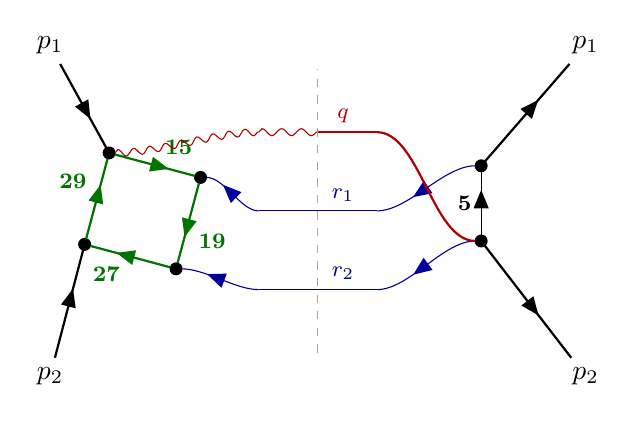
\begin{tikzpicture}
\begin{feynman}
\vertex (Lp1) at (-3.400,2.100) {$p_1$};
\vertex (Lp2) at (-3.400,-2.100) {$p_2$};
\vertex (Lcr1) at (-0.750,0.000);
\vertex (Lcr2) at (-0.750,-1.000);
\vertex (Lcq) at (-0.750,1.000);
\vertex (Mq) at (0,1.000);
\vertex[dot] (Lv0) at (-2.650,0.736) {};
\vertex[dot] (Lv1) at (-1.489,0.425) {};
\vertex[dot] (Lv2) at (-1.800,-0.736) {};
\vertex[dot] (Lv3) at (-2.961,-0.425) {};
\vertex (Rp1) at (3.400,2.100) {$p_1$};
\vertex (Rp2) at (3.400,-2.100) {$p_2$};
\vertex (Rcr1) at (0.750,0.000);
\vertex (Rcr2) at (0.750,-1.000);
\vertex (Rcq) at (0.750,1.000);
\vertex[dot] (R5) at (2.075,0.573) {};
\vertex[dot] (Rroot) at (2.075,-0.382) {};
\diagram* {
(Lv0) -- [plain, thick, green!45!black, with arrow=0.55, edge label={\footnotesize\bfseries 15}] (Lv1),
(Lv1) -- [plain, thick, green!45!black, with arrow=0.55, edge label={\footnotesize\bfseries 19}] (Lv2),
(Lv2) -- [plain, thick, green!45!black, with arrow=0.55, edge label={\footnotesize\bfseries 27}] (Lv3),
(Lv3) -- [plain, thick, green!45!black, with arrow=0.55, edge label={\footnotesize\bfseries 29}] (Lv0),
(Lcq) -- [boson, red!70!black, out=180, in=0, looseness=0.75] (Lv0),
(Lp1) -- [plain, thick, with arrow=0.55] (Lv0),
(Lcr1) -- [plain, blue!60!black, out=180, in=0, looseness=0.75, with arrow=0.55] (Lv1),
(Lcr2) -- [plain, blue!60!black, out=180, in=0, looseness=0.75, with arrow=0.55] (Lv2),
(Lp2) -- [plain, thick, with arrow=0.55] (Lv3),
(Rroot) -- [plain, with arrow=0.55, edge label={\footnotesize\bfseries 5}] (R5),
(R5) -- [plain, thick, with arrow=0.55] (Rp1),
(Rroot) -- [plain, thick, with arrow=0.55] (Rp2),
(R5) -- [plain, blue!60!black, out=180, in=0, looseness=0.75, with arrow=0.55] (Rcr1),
(Rroot) -- [plain, blue!60!black, out=180, in=0, looseness=0.75, with arrow=0.55] (Rcr2),
(Rroot) -- [plain, red!70!black, double, double distance=1.2pt, thick, out=180, in=0, looseness=0.75] (Rcq),
(Rcr1) -- [plain, blue!60!black] (Lcr1),
(Rcr2) -- [plain, blue!60!black] (Lcr2),
(Rcq) -- [plain, red!70!black, double, double distance=1.2pt, thick] (Mq) -- [boson, red!70!black] (Lcq),
};
\end{feynman}
\draw[dashed, gray!70] (0,-1.80) -- (0,1.80);
\node[font=\footnotesize, blue!60!black, above] at (0.32,0.00) {$r_1$};
\node[font=\footnotesize, blue!60!black, above] at (0.32,-1.00) {$r_2$};
\node[font=\footnotesize, red!70!black, above] at (0.32,1.00) {$q$};
\end{tikzpicture}}\\[2mm]\textbf{topo3} (RR family 8, pentagon q-p1-r1-r2-p2), sector with 5 of 8 lines\\[2pt]{\footnotesize\begin{tabular}{@{}r@{\ \ }l@{\ \ }l@{}}\textbf{15} & $(k_1+p_1)^2$ & loop\\
\textbf{19} & $(k_1+p_1+r_1)^2$ & loop\\
\textbf{27} & $(k_1+p_1+r_1+r_2)^2$ & loop\\
\textbf{29} & $(k_1+p_1+p_2+r_1+r_2)^2$ & loop\\
\textbf{5} & $(p_1+r_1)^2$ & conjugate\\\end{tabular}}\\[2pt]{\scriptsize pinched: 8 = $(p_2+r_2)^2$, 11 = $(r_1+r_2)^2$, 14 = $(k_1)^2$}\end{minipage}\hfill%
\begin{minipage}[t]{0.48\textwidth}\centering\resizebox{0.9\linewidth}{!}{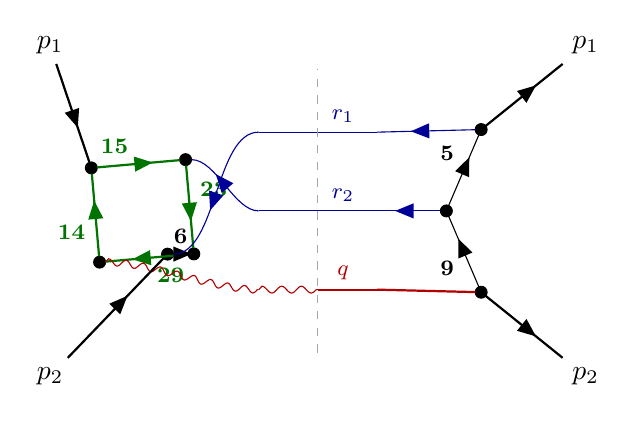
\begin{tikzpicture}
\begin{feynman}
\vertex (Lp1) at (-3.400,2.100) {$p_1$};
\vertex (Lp2) at (-3.400,-2.100) {$p_2$};
\vertex (Lcr1) at (-0.750,1.000);
\vertex (Lcr2) at (-0.750,0.000);
\vertex (Lcq) at (-0.750,-1.000);
\vertex (Mq) at (0,-1.000);
\vertex[dot] (Lv0) at (-2.771,-0.651) {};
\vertex[dot] (Lv1) at (-2.876,0.546) {};
\vertex[dot] (Lv2) at (-1.679,0.651) {};
\vertex[dot] (Lv3) at (-1.574,-0.546) {};
\vertex[dot] (Lt6) at (-1.908,-0.549) {};
\vertex (Rp1) at (3.400,2.100) {$p_1$};
\vertex (Rp2) at (3.400,-2.100) {$p_2$};
\vertex (Rcr1) at (0.750,1.000);
\vertex (Rcr2) at (0.750,0.000);
\vertex (Rcq) at (0.750,-1.000);
\vertex[dot] (R5) at (2.075,1.033) {};
\vertex[dot] (R9) at (1.633,0.000) {};
\vertex[dot] (Rroot) at (2.075,-1.033) {};
\diagram* {
(Lv0) -- [plain, thick, green!45!black, with arrow=0.55, edge label={\footnotesize\bfseries 14}] (Lv1),
(Lv1) -- [plain, thick, green!45!black, with arrow=0.55, edge label={\footnotesize\bfseries 15}] (Lv2),
(Lv2) -- [plain, thick, green!45!black, with arrow=0.55, edge label={\footnotesize\bfseries 23}] (Lv3),
(Lv3) -- [plain, thick, green!45!black, with arrow=0.55, edge label={\footnotesize\bfseries 29}] (Lv0),
(Lcq) -- [boson, red!70!black, out=180, in=0, looseness=0.75] (Lv0),
(Lp1) -- [plain, thick, with arrow=0.55] (Lv1),
(Lcr2) -- [plain, blue!60!black, out=180, in=0, looseness=0.75, with arrow=0.55] (Lv2),
(Lt6) -- [plain, with arrow=0.55, edge label={\footnotesize\bfseries 6}] (Lv3),
(Lp2) -- [plain, thick, with arrow=0.55] (Lt6),
(Lcr1) -- [plain, blue!60!black, out=180, in=0, looseness=0.75, with arrow=0.55] (Lt6),
(R9) -- [plain, with arrow=0.55, edge label={\footnotesize\bfseries 5}] (R5),
(Rroot) -- [plain, with arrow=0.55, edge label={\footnotesize\bfseries 9}] (R9),
(R5) -- [plain, thick, with arrow=0.55] (Rp1),
(Rroot) -- [plain, thick, with arrow=0.55] (Rp2),
(R5) -- [plain, blue!60!black, with arrow=0.55] (Rcr1),
(R9) -- [plain, blue!60!black, with arrow=0.55] (Rcr2),
(Rroot) -- [plain, red!70!black, double, double distance=1.2pt, thick] (Rcq),
(Rcr1) -- [plain, blue!60!black] (Lcr1),
(Rcr2) -- [plain, blue!60!black] (Lcr2),
(Rcq) -- [plain, red!70!black, double, double distance=1.2pt, thick] (Mq) -- [boson, red!70!black] (Lcq),
};
\end{feynman}
\draw[dashed, gray!70] (0,-1.80) -- (0,1.80);
\node[font=\footnotesize, blue!60!black, above] at (0.32,1.00) {$r_1$};
\node[font=\footnotesize, blue!60!black, above] at (0.32,0.00) {$r_2$};
\node[font=\footnotesize, red!70!black, above] at (0.32,-1.00) {$q$};
\end{tikzpicture}}\\[2mm]\textbf{topo4} (RR family 3, pentagon q-p1-r2-r1-p2), sector with 7 of 8 lines\\[2pt]{\footnotesize\begin{tabular}{@{}r@{\ \ }l@{\ \ }l@{}}\textbf{14} & $(k_1)^2$ & loop\\
\textbf{15} & $(k_1+p_1)^2$ & loop\\
\textbf{23} & $(k_1+p_1+r_2)^2$ & loop\\
\textbf{29} & $(k_1+p_1+p_2+r_1+r_2)^2$ & loop\\
\textbf{6} & $(p_2+r_1)^2$ & amplitude (tree on the loop)\\
\textbf{5} & $(p_1+r_1)^2$ & conjugate\\
\textbf{9} & $(p_1+r_1+r_2)^2$ & conjugate\\\end{tabular}}\\[2pt]{\scriptsize pinched: 27 = $(k_1+p_1+r_1+r_2)^2$}\end{minipage}

\bigskip

\begin{minipage}[t]{0.48\textwidth}\centering\resizebox{0.9\linewidth}{!}{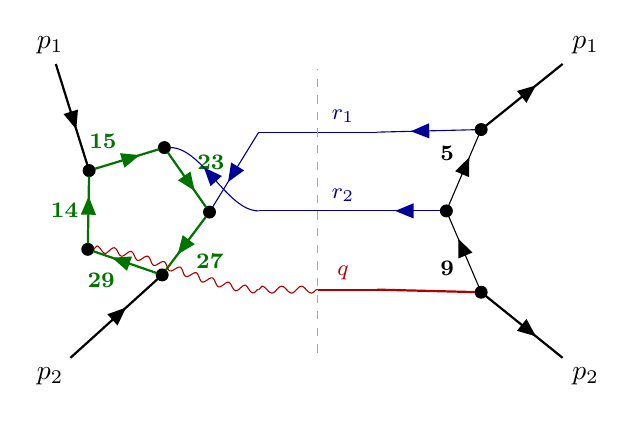
\begin{tikzpicture}
\begin{feynman}
\vertex (Lp1) at (-3.400,2.100) {$p_1$};
\vertex (Lp2) at (-3.400,-2.100) {$p_2$};
\vertex (Lcr1) at (-0.750,1.000);
\vertex (Lcr2) at (-0.750,0.000);
\vertex (Lcq) at (-0.750,-1.000);
\vertex (Mq) at (0,-1.000);
\vertex[dot] (Lv0) at (-2.921,-0.488) {};
\vertex[dot] (Lv1) at (-2.904,0.512) {};
\vertex[dot] (Lv2) at (-1.948,0.804) {};
\vertex[dot] (Lv3) at (-1.375,-0.015) {};
\vertex[dot] (Lv4) at (-1.976,-0.813) {};
\vertex (Rp1) at (3.400,2.100) {$p_1$};
\vertex (Rp2) at (3.400,-2.100) {$p_2$};
\vertex (Rcr1) at (0.750,1.000);
\vertex (Rcr2) at (0.750,0.000);
\vertex (Rcq) at (0.750,-1.000);
\vertex[dot] (R5) at (2.075,1.033) {};
\vertex[dot] (R9) at (1.633,0.000) {};
\vertex[dot] (Rroot) at (2.075,-1.033) {};
\diagram* {
(Lv0) -- [plain, thick, green!45!black, with arrow=0.55, edge label={\footnotesize\bfseries 14}] (Lv1),
(Lv1) -- [plain, thick, green!45!black, with arrow=0.55, edge label={\footnotesize\bfseries 15}] (Lv2),
(Lv2) -- [plain, thick, green!45!black, with arrow=0.55, edge label={\footnotesize\bfseries 23}] (Lv3),
(Lv3) -- [plain, thick, green!45!black, with arrow=0.55, edge label={\footnotesize\bfseries 27}] (Lv4),
(Lv4) -- [plain, thick, green!45!black, with arrow=0.55, edge label={\footnotesize\bfseries 29}] (Lv0),
(Lcq) -- [boson, red!70!black, out=180, in=0, looseness=0.75] (Lv0),
(Lp1) -- [plain, thick, with arrow=0.55] (Lv1),
(Lcr2) -- [plain, blue!60!black, out=180, in=0, looseness=0.75, with arrow=0.55] (Lv2),
(Lcr1) -- [plain, blue!60!black, with arrow=0.55] (Lv3),
(Lp2) -- [plain, thick, with arrow=0.55] (Lv4),
(R9) -- [plain, with arrow=0.55, edge label={\footnotesize\bfseries 5}] (R5),
(Rroot) -- [plain, with arrow=0.55, edge label={\footnotesize\bfseries 9}] (R9),
(R5) -- [plain, thick, with arrow=0.55] (Rp1),
(Rroot) -- [plain, thick, with arrow=0.55] (Rp2),
(R5) -- [plain, blue!60!black, with arrow=0.55] (Rcr1),
(R9) -- [plain, blue!60!black, with arrow=0.55] (Rcr2),
(Rroot) -- [plain, red!70!black, double, double distance=1.2pt, thick] (Rcq),
(Rcr1) -- [plain, blue!60!black] (Lcr1),
(Rcr2) -- [plain, blue!60!black] (Lcr2),
(Rcq) -- [plain, red!70!black, double, double distance=1.2pt, thick] (Mq) -- [boson, red!70!black] (Lcq),
};
\end{feynman}
\draw[dashed, gray!70] (0,-1.80) -- (0,1.80);
\node[font=\footnotesize, blue!60!black, above] at (0.32,1.00) {$r_1$};
\node[font=\footnotesize, blue!60!black, above] at (0.32,0.00) {$r_2$};
\node[font=\footnotesize, red!70!black, above] at (0.32,-1.00) {$q$};
\end{tikzpicture}}\\[2mm]\textbf{topo4} (RR family 3, pentagon q-p1-r2-r1-p2), sector with 7 of 8 lines\\[2pt]{\footnotesize\begin{tabular}{@{}r@{\ \ }l@{\ \ }l@{}}\textbf{14} & $(k_1)^2$ & loop\\
\textbf{15} & $(k_1+p_1)^2$ & loop\\
\textbf{23} & $(k_1+p_1+r_2)^2$ & loop\\
\textbf{27} & $(k_1+p_1+r_1+r_2)^2$ & loop\\
\textbf{29} & $(k_1+p_1+p_2+r_1+r_2)^2$ & loop\\
\textbf{5} & $(p_1+r_1)^2$ & conjugate\\
\textbf{9} & $(p_1+r_1+r_2)^2$ & conjugate\\\end{tabular}}\\[2pt]{\scriptsize pinched: 6 = $(p_2+r_1)^2$}\end{minipage}\hfill%
\begin{minipage}[t]{0.48\textwidth}\centering\resizebox{0.9\linewidth}{!}{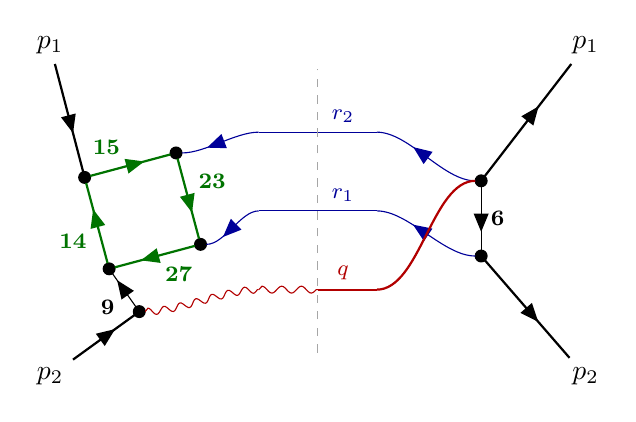
\begin{tikzpicture}
\begin{feynman}
\vertex (Lp1) at (-3.400,2.100) {$p_1$};
\vertex (Lp2) at (-3.400,-2.100) {$p_2$};
\vertex (Lcr1) at (-0.750,0.000);
\vertex (Lcr2) at (-0.750,1.000);
\vertex (Lcq) at (-0.750,-1.000);
\vertex (Mq) at (0,-1.000);
\vertex[dot] (Lv0) at (-2.650,-0.736) {};
\vertex[dot] (Lv1) at (-2.961,0.425) {};
\vertex[dot] (Lv2) at (-1.800,0.736) {};
\vertex[dot] (Lv3) at (-1.489,-0.425) {};
\vertex[dot] (Lt9) at (-2.267,-1.279) {};
\vertex (Rp1) at (3.400,2.100) {$p_1$};
\vertex (Rp2) at (3.400,-2.100) {$p_2$};
\vertex (Rcr1) at (0.750,0.000);
\vertex (Rcr2) at (0.750,1.000);
\vertex (Rcq) at (0.750,-1.000);
\vertex[dot] (R6) at (2.075,-0.573) {};
\vertex[dot] (Rroot) at (2.075,0.382) {};
\diagram* {
(Lv0) -- [plain, thick, green!45!black, with arrow=0.55, edge label={\footnotesize\bfseries 14}] (Lv1),
(Lv1) -- [plain, thick, green!45!black, with arrow=0.55, edge label={\footnotesize\bfseries 15}] (Lv2),
(Lv2) -- [plain, thick, green!45!black, with arrow=0.55, edge label={\footnotesize\bfseries 23}] (Lv3),
(Lv3) -- [plain, thick, green!45!black, with arrow=0.55, edge label={\footnotesize\bfseries 27}] (Lv0),
(Lt9) -- [plain, with arrow=0.55, edge label={\footnotesize\bfseries 9}] (Lv0),
(Lp2) -- [plain, thick, with arrow=0.55] (Lt9),
(Lcq) -- [boson, red!70!black, out=180, in=0, looseness=0.75] (Lt9),
(Lp1) -- [plain, thick, with arrow=0.55] (Lv1),
(Lcr2) -- [plain, blue!60!black, out=180, in=0, looseness=0.75, with arrow=0.55] (Lv2),
(Lcr1) -- [plain, blue!60!black, out=180, in=0, looseness=0.75, with arrow=0.55] (Lv3),
(Rroot) -- [plain, with arrow=0.55, edge label={\footnotesize\bfseries 6}] (R6),
(Rroot) -- [plain, thick, with arrow=0.55] (Rp1),
(R6) -- [plain, thick, with arrow=0.55] (Rp2),
(R6) -- [plain, blue!60!black, out=180, in=0, looseness=0.75, with arrow=0.55] (Rcr1),
(Rroot) -- [plain, blue!60!black, out=180, in=0, looseness=0.75, with arrow=0.55] (Rcr2),
(Rroot) -- [plain, red!70!black, double, double distance=1.2pt, thick, out=180, in=0, looseness=0.75] (Rcq),
(Rcr1) -- [plain, blue!60!black] (Lcr1),
(Rcr2) -- [plain, blue!60!black] (Lcr2),
(Rcq) -- [plain, red!70!black, double, double distance=1.2pt, thick] (Mq) -- [boson, red!70!black] (Lcq),
};
\end{feynman}
\draw[dashed, gray!70] (0,-1.80) -- (0,1.80);
\node[font=\footnotesize, blue!60!black, above] at (0.32,0.00) {$r_1$};
\node[font=\footnotesize, blue!60!black, above] at (0.32,1.00) {$r_2$};
\node[font=\footnotesize, red!70!black, above] at (0.32,-1.00) {$q$};
\end{tikzpicture}}\\[2mm]\textbf{topo4} (RR family 3, pentagon q-p1-r2-r1-p2), sector with 6 of 8 lines\\[2pt]{\footnotesize\begin{tabular}{@{}r@{\ \ }l@{\ \ }l@{}}\textbf{14} & $(k_1)^2$ & loop\\
\textbf{15} & $(k_1+p_1)^2$ & loop\\
\textbf{23} & $(k_1+p_1+r_2)^2$ & loop\\
\textbf{27} & $(k_1+p_1+r_1+r_2)^2$ & loop\\
\textbf{9} & $(p_1+r_1+r_2)^2$ & amplitude (tree on the loop)\\
\textbf{6} & $(p_2+r_1)^2$ & conjugate\\\end{tabular}}\\[2pt]{\scriptsize pinched: 5 = $(p_1+r_1)^2$, 29 = $(k_1+p_1+p_2+r_1+r_2)^2$}\end{minipage}

\bigskip

\begin{minipage}[t]{0.48\textwidth}\centering\resizebox{0.9\linewidth}{!}{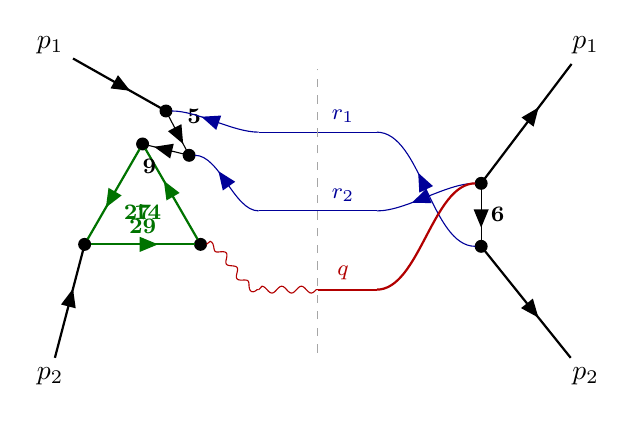
\begin{tikzpicture}
\begin{feynman}
\vertex (Lp1) at (-3.400,2.100) {$p_1$};
\vertex (Lp2) at (-3.400,-2.100) {$p_2$};
\vertex (Lcr1) at (-0.750,1.000);
\vertex (Lcr2) at (-0.750,0.000);
\vertex (Lcq) at (-0.750,-1.000);
\vertex (Mq) at (0,-1.000);
\vertex[dot] (Lv0) at (-1.489,-0.425) {};
\vertex[dot] (Lv1) at (-2.225,0.850) {};
\vertex[dot] (Lv2) at (-2.961,-0.425) {};
\vertex[dot] (Lt5) at (-1.928,1.269) {};
\vertex[dot] (Lt9) at (-1.634,0.706) {};
\vertex (Rp1) at (3.400,2.100) {$p_1$};
\vertex (Rp2) at (3.400,-2.100) {$p_2$};
\vertex (Rcr1) at (0.750,1.000);
\vertex (Rcr2) at (0.750,0.000);
\vertex (Rcq) at (0.750,-1.000);
\vertex[dot] (R6) at (2.075,-0.450) {};
\vertex[dot] (Rroot) at (2.075,0.350) {};
\diagram* {
(Lv0) -- [plain, thick, green!45!black, with arrow=0.55, edge label={\footnotesize\bfseries 14}] (Lv1),
(Lv1) -- [plain, thick, green!45!black, with arrow=0.55, edge label={\footnotesize\bfseries 27}] (Lv2),
(Lv2) -- [plain, thick, green!45!black, with arrow=0.55, edge label={\footnotesize\bfseries 29}] (Lv0),
(Lcq) -- [boson, red!70!black, out=180, in=0, looseness=0.75] (Lv0),
(Lt5) -- [plain, with arrow=0.55, edge label={\footnotesize\bfseries 5}] (Lt9),
(Lt9) -- [plain, with arrow=0.55, edge label={\footnotesize\bfseries 9}] (Lv1),
(Lcr1) -- [plain, blue!60!black, out=180, in=0, looseness=0.75, with arrow=0.55] (Lt5),
(Lcr2) -- [plain, blue!60!black, out=180, in=0, looseness=0.75, with arrow=0.55] (Lt9),
(Lp1) -- [plain, thick, with arrow=0.55] (Lt5),
(Lp2) -- [plain, thick, with arrow=0.55] (Lv2),
(Rroot) -- [plain, with arrow=0.55, edge label={\footnotesize\bfseries 6}] (R6),
(Rroot) -- [plain, thick, with arrow=0.55] (Rp1),
(R6) -- [plain, thick, with arrow=0.55] (Rp2),
(R6) -- [plain, blue!60!black, out=180, in=0, looseness=0.75, with arrow=0.55] (Rcr1),
(Rroot) -- [plain, blue!60!black, out=180, in=0, looseness=0.75, with arrow=0.55] (Rcr2),
(Rroot) -- [plain, red!70!black, double, double distance=1.2pt, thick, out=180, in=0, looseness=0.75] (Rcq),
(Rcr1) -- [plain, blue!60!black] (Lcr1),
(Rcr2) -- [plain, blue!60!black] (Lcr2),
(Rcq) -- [plain, red!70!black, double, double distance=1.2pt, thick] (Mq) -- [boson, red!70!black] (Lcq),
};
\end{feynman}
\draw[dashed, gray!70] (0,-1.80) -- (0,1.80);
\node[font=\footnotesize, blue!60!black, above] at (0.32,1.00) {$r_1$};
\node[font=\footnotesize, blue!60!black, above] at (0.32,0.00) {$r_2$};
\node[font=\footnotesize, red!70!black, above] at (0.32,-1.00) {$q$};
\end{tikzpicture}}\\[2mm]\textbf{topo4} (RR family 3, pentagon q-p1-r2-r1-p2), sector with 6 of 8 lines\\[2pt]{\footnotesize\begin{tabular}{@{}r@{\ \ }l@{\ \ }l@{}}\textbf{14} & $(k_1)^2$ & loop\\
\textbf{27} & $(k_1+p_1+r_1+r_2)^2$ & loop\\
\textbf{29} & $(k_1+p_1+p_2+r_1+r_2)^2$ & loop\\
\textbf{5} & $(p_1+r_1)^2$ & amplitude (tree on the loop)\\
\textbf{9} & $(p_1+r_1+r_2)^2$ & amplitude (tree on the loop)\\
\textbf{6} & $(p_2+r_1)^2$ & conjugate\\\end{tabular}}\\[2pt]{\scriptsize pinched: 15 = $(k_1+p_1)^2$, 23 = $(k_1+p_1+r_2)^2$}\end{minipage}\hfill%
\begin{minipage}[t]{0.48\textwidth}\centering\resizebox{0.9\linewidth}{!}{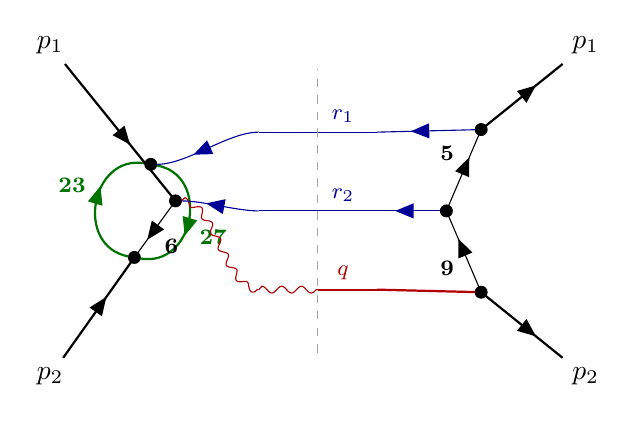
\begin{tikzpicture}
\begin{feynman}
\vertex (Lp1) at (-3.400,2.100) {$p_1$};
\vertex (Lp2) at (-3.400,-2.100) {$p_2$};
\vertex (Lcr1) at (-0.750,1.000);
\vertex (Lcr2) at (-0.750,0.000);
\vertex (Lcq) at (-0.750,-1.000);
\vertex (Mq) at (0,-1.000);
\vertex[dot] (Lv0) at (-2.329,-0.591) {};
\vertex[dot] (Lv1) at (-2.121,0.591) {};
\vertex[dot] (Lt6) at (-1.807,0.127) {};
\vertex (Rp1) at (3.400,2.100) {$p_1$};
\vertex (Rp2) at (3.400,-2.100) {$p_2$};
\vertex (Rcr1) at (0.750,1.000);
\vertex (Rcr2) at (0.750,0.000);
\vertex (Rcq) at (0.750,-1.000);
\vertex[dot] (R5) at (2.075,1.033) {};
\vertex[dot] (R9) at (1.633,0.000) {};
\vertex[dot] (Rroot) at (2.075,-1.033) {};
\diagram* {
(Lv0) -- [plain, thick, green!45!black, half left, with arrow=0.55, edge label={\footnotesize\bfseries 23}] (Lv1),
(Lv1) -- [plain, thick, green!45!black, half left, with arrow=0.55, edge label={\footnotesize\bfseries 27}] (Lv0),
(Lt6) -- [plain, with arrow=0.55, edge label={\footnotesize\bfseries 6}] (Lv0),
(Lp2) -- [plain, thick, with arrow=0.55] (Lv0),
(Lcq) -- [boson, red!70!black, out=180, in=0, looseness=0.75] (Lt6),
(Lcr2) -- [plain, blue!60!black, out=180, in=0, looseness=0.75, with arrow=0.55] (Lt6),
(Lp1) -- [plain, thick, with arrow=0.55] (Lt6),
(Lcr1) -- [plain, blue!60!black, out=180, in=0, looseness=0.75, with arrow=0.55] (Lv1),
(R9) -- [plain, with arrow=0.55, edge label={\footnotesize\bfseries 5}] (R5),
(Rroot) -- [plain, with arrow=0.55, edge label={\footnotesize\bfseries 9}] (R9),
(R5) -- [plain, thick, with arrow=0.55] (Rp1),
(Rroot) -- [plain, thick, with arrow=0.55] (Rp2),
(R5) -- [plain, blue!60!black, with arrow=0.55] (Rcr1),
(R9) -- [plain, blue!60!black, with arrow=0.55] (Rcr2),
(Rroot) -- [plain, red!70!black, double, double distance=1.2pt, thick] (Rcq),
(Rcr1) -- [plain, blue!60!black] (Lcr1),
(Rcr2) -- [plain, blue!60!black] (Lcr2),
(Rcq) -- [plain, red!70!black, double, double distance=1.2pt, thick] (Mq) -- [boson, red!70!black] (Lcq),
};
\end{feynman}
\draw[dashed, gray!70] (0,-1.80) -- (0,1.80);
\node[font=\footnotesize, blue!60!black, above] at (0.32,1.00) {$r_1$};
\node[font=\footnotesize, blue!60!black, above] at (0.32,0.00) {$r_2$};
\node[font=\footnotesize, red!70!black, above] at (0.32,-1.00) {$q$};
\end{tikzpicture}}\\[2mm]\textbf{topo4} (RR family 3, pentagon q-p1-r2-r1-p2), sector with 5 of 8 lines\\[2pt]{\footnotesize\begin{tabular}{@{}r@{\ \ }l@{\ \ }l@{}}\textbf{23} & $(k_1+p_1+r_2)^2$ & loop\\
\textbf{27} & $(k_1+p_1+r_1+r_2)^2$ & loop\\
\textbf{6} & $(p_2+r_1)^2$ & amplitude (tree on the loop)\\
\textbf{5} & $(p_1+r_1)^2$ & conjugate\\
\textbf{9} & $(p_1+r_1+r_2)^2$ & conjugate\\\end{tabular}}\\[2pt]{\scriptsize pinched: 14 = $(k_1)^2$, 15 = $(k_1+p_1)^2$, 29 = $(k_1+p_1+p_2+r_1+r_2)^2$}\end{minipage}

\bigskip

\begin{minipage}[t]{0.48\textwidth}\centering\resizebox{0.9\linewidth}{!}{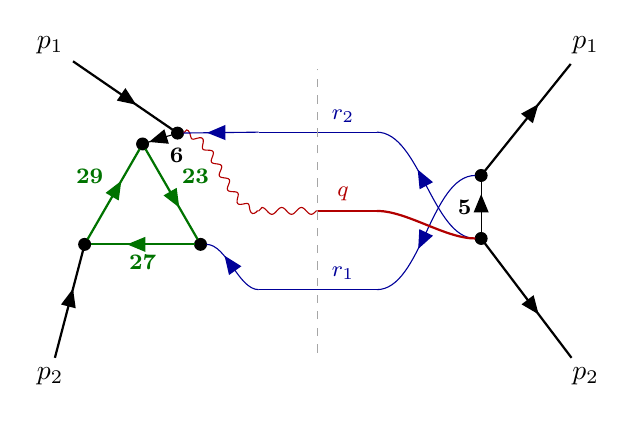
\begin{tikzpicture}
\begin{feynman}
\vertex (Lp1) at (-3.400,2.100) {$p_1$};
\vertex (Lp2) at (-3.400,-2.100) {$p_2$};
\vertex (Lcr1) at (-0.750,-1.000);
\vertex (Lcr2) at (-0.750,1.000);
\vertex (Lcq) at (-0.750,0.000);
\vertex (Mq) at (0,0.000);
\vertex[dot] (Lv0) at (-2.225,0.850) {};
\vertex[dot] (Lv1) at (-1.489,-0.425) {};
\vertex[dot] (Lv2) at (-2.961,-0.425) {};
\vertex[dot] (Lt6) at (-1.781,0.988) {};
\vertex (Rp1) at (3.400,2.100) {$p_1$};
\vertex (Rp2) at (3.400,-2.100) {$p_2$};
\vertex (Rcr1) at (0.750,-1.000);
\vertex (Rcr2) at (0.750,1.000);
\vertex (Rcq) at (0.750,0.000);
\vertex[dot] (R5) at (2.075,0.450) {};
\vertex[dot] (Rroot) at (2.075,-0.350) {};
\diagram* {
(Lv0) -- [plain, thick, green!45!black, with arrow=0.55, edge label={\footnotesize\bfseries 23}] (Lv1),
(Lv1) -- [plain, thick, green!45!black, with arrow=0.55, edge label={\footnotesize\bfseries 27}] (Lv2),
(Lv2) -- [plain, thick, green!45!black, with arrow=0.55, edge label={\footnotesize\bfseries 29}] (Lv0),
(Lt6) -- [plain, with arrow=0.55, edge label={\footnotesize\bfseries 6}] (Lv0),
(Lcq) -- [boson, red!70!black, out=180, in=0, looseness=0.75] (Lt6),
(Lcr2) -- [plain, blue!60!black, with arrow=0.55] (Lt6),
(Lp1) -- [plain, thick, with arrow=0.55] (Lt6),
(Lcr1) -- [plain, blue!60!black, out=180, in=0, looseness=0.75, with arrow=0.55] (Lv1),
(Lp2) -- [plain, thick, with arrow=0.55] (Lv2),
(Rroot) -- [plain, with arrow=0.55, edge label={\footnotesize\bfseries 5}] (R5),
(R5) -- [plain, thick, with arrow=0.55] (Rp1),
(Rroot) -- [plain, thick, with arrow=0.55] (Rp2),
(R5) -- [plain, blue!60!black, out=180, in=0, looseness=0.75, with arrow=0.55] (Rcr1),
(Rroot) -- [plain, blue!60!black, out=180, in=0, looseness=0.75, with arrow=0.55] (Rcr2),
(Rroot) -- [plain, red!70!black, double, double distance=1.2pt, thick, out=180, in=0, looseness=0.75] (Rcq),
(Rcr1) -- [plain, blue!60!black] (Lcr1),
(Rcr2) -- [plain, blue!60!black] (Lcr2),
(Rcq) -- [plain, red!70!black, double, double distance=1.2pt, thick] (Mq) -- [boson, red!70!black] (Lcq),
};
\end{feynman}
\draw[dashed, gray!70] (0,-1.80) -- (0,1.80);
\node[font=\footnotesize, blue!60!black, above] at (0.32,-1.00) {$r_1$};
\node[font=\footnotesize, blue!60!black, above] at (0.32,1.00) {$r_2$};
\node[font=\footnotesize, red!70!black, above] at (0.32,0.00) {$q$};
\end{tikzpicture}}\\[2mm]\textbf{topo4} (RR family 3, pentagon q-p1-r2-r1-p2), sector with 5 of 8 lines\\[2pt]{\footnotesize\begin{tabular}{@{}r@{\ \ }l@{\ \ }l@{}}\textbf{23} & $(k_1+p_1+r_2)^2$ & loop\\
\textbf{27} & $(k_1+p_1+r_1+r_2)^2$ & loop\\
\textbf{29} & $(k_1+p_1+p_2+r_1+r_2)^2$ & loop\\
\textbf{6} & $(p_2+r_1)^2$ & amplitude (tree on the loop)\\
\textbf{5} & $(p_1+r_1)^2$ & conjugate\\\end{tabular}}\\[2pt]{\scriptsize pinched: 9 = $(p_1+r_1+r_2)^2$, 14 = $(k_1)^2$, 15 = $(k_1+p_1)^2$}\end{minipage}\hfill%
\begin{minipage}[t]{0.48\textwidth}\centering\resizebox{0.9\linewidth}{!}{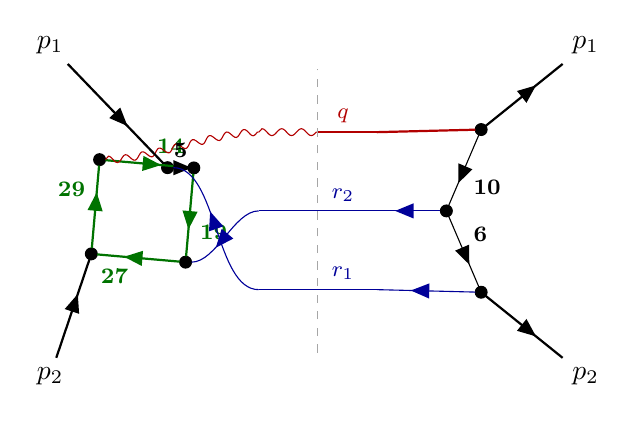
\begin{tikzpicture}
\begin{feynman}
\vertex (Lp1) at (-3.400,2.100) {$p_1$};
\vertex (Lp2) at (-3.400,-2.100) {$p_2$};
\vertex (Lcr1) at (-0.750,-1.000);
\vertex (Lcr2) at (-0.750,0.000);
\vertex (Lcq) at (-0.750,1.000);
\vertex (Mq) at (0,1.000);
\vertex[dot] (Lv0) at (-2.771,0.651) {};
\vertex[dot] (Lv1) at (-1.574,0.546) {};
\vertex[dot] (Lv2) at (-1.679,-0.651) {};
\vertex[dot] (Lv3) at (-2.876,-0.546) {};
\vertex[dot] (Lt5) at (-1.908,0.549) {};
\vertex (Rp1) at (3.400,2.100) {$p_1$};
\vertex (Rp2) at (3.400,-2.100) {$p_2$};
\vertex (Rcr1) at (0.750,-1.000);
\vertex (Rcr2) at (0.750,0.000);
\vertex (Rcq) at (0.750,1.000);
\vertex[dot] (R6) at (2.075,-1.033) {};
\vertex[dot] (R10) at (1.633,0.000) {};
\vertex[dot] (Rroot) at (2.075,1.033) {};
\diagram* {
(Lv0) -- [plain, thick, green!45!black, with arrow=0.55, edge label={\footnotesize\bfseries 14}] (Lv1),
(Lv1) -- [plain, thick, green!45!black, with arrow=0.55, edge label={\footnotesize\bfseries 19}] (Lv2),
(Lv2) -- [plain, thick, green!45!black, with arrow=0.55, edge label={\footnotesize\bfseries 27}] (Lv3),
(Lv3) -- [plain, thick, green!45!black, with arrow=0.55, edge label={\footnotesize\bfseries 29}] (Lv0),
(Lcq) -- [boson, red!70!black, out=180, in=0, looseness=0.75] (Lv0),
(Lt5) -- [plain, with arrow=0.55, edge label={\footnotesize\bfseries 5}] (Lv1),
(Lcr1) -- [plain, blue!60!black, out=180, in=0, looseness=0.75, with arrow=0.55] (Lt5),
(Lp1) -- [plain, thick, with arrow=0.55] (Lt5),
(Lcr2) -- [plain, blue!60!black, out=180, in=0, looseness=0.75, with arrow=0.55] (Lv2),
(Lp2) -- [plain, thick, with arrow=0.55] (Lv3),
(R10) -- [plain, with arrow=0.55, edge label={\footnotesize\bfseries 6}] (R6),
(Rroot) -- [plain, with arrow=0.55, edge label={\footnotesize\bfseries 10}] (R10),
(Rroot) -- [plain, thick, with arrow=0.55] (Rp1),
(R6) -- [plain, thick, with arrow=0.55] (Rp2),
(R6) -- [plain, blue!60!black, with arrow=0.55] (Rcr1),
(R10) -- [plain, blue!60!black, with arrow=0.55] (Rcr2),
(Rroot) -- [plain, red!70!black, double, double distance=1.2pt, thick] (Rcq),
(Rcr1) -- [plain, blue!60!black] (Lcr1),
(Rcr2) -- [plain, blue!60!black] (Lcr2),
(Rcq) -- [plain, red!70!black, double, double distance=1.2pt, thick] (Mq) -- [boson, red!70!black] (Lcq),
};
\end{feynman}
\draw[dashed, gray!70] (0,-1.80) -- (0,1.80);
\node[font=\footnotesize, blue!60!black, above] at (0.32,-1.00) {$r_1$};
\node[font=\footnotesize, blue!60!black, above] at (0.32,0.00) {$r_2$};
\node[font=\footnotesize, red!70!black, above] at (0.32,1.00) {$q$};
\end{tikzpicture}}\\[2mm]\textbf{topo5} (RR family 4, pentagon q-p1-r1-r2-p2), sector with 7 of 8 lines\\[2pt]{\footnotesize\begin{tabular}{@{}r@{\ \ }l@{\ \ }l@{}}\textbf{14} & $(k_1)^2$ & loop\\
\textbf{19} & $(k_1+p_1+r_1)^2$ & loop\\
\textbf{27} & $(k_1+p_1+r_1+r_2)^2$ & loop\\
\textbf{29} & $(k_1+p_1+p_2+r_1+r_2)^2$ & loop\\
\textbf{5} & $(p_1+r_1)^2$ & amplitude (tree on the loop)\\
\textbf{6} & $(p_2+r_1)^2$ & conjugate\\
\textbf{10} & $(p_2+r_1+r_2)^2$ & conjugate\\\end{tabular}}\\[2pt]{\scriptsize pinched: 15 = $(k_1+p_1)^2$}\end{minipage}

\bigskip

\begin{minipage}[t]{0.48\textwidth}\centering\resizebox{0.9\linewidth}{!}{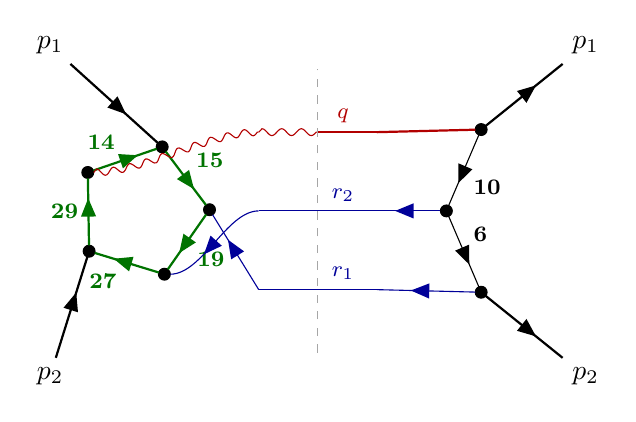
\begin{tikzpicture}
\begin{feynman}
\vertex (Lp1) at (-3.400,2.100) {$p_1$};
\vertex (Lp2) at (-3.400,-2.100) {$p_2$};
\vertex (Lcr1) at (-0.750,-1.000);
\vertex (Lcr2) at (-0.750,0.000);
\vertex (Lcq) at (-0.750,1.000);
\vertex (Mq) at (0,1.000);
\vertex[dot] (Lv0) at (-2.921,0.488) {};
\vertex[dot] (Lv1) at (-1.976,0.813) {};
\vertex[dot] (Lv2) at (-1.375,0.015) {};
\vertex[dot] (Lv3) at (-1.948,-0.804) {};
\vertex[dot] (Lv4) at (-2.904,-0.512) {};
\vertex (Rp1) at (3.400,2.100) {$p_1$};
\vertex (Rp2) at (3.400,-2.100) {$p_2$};
\vertex (Rcr1) at (0.750,-1.000);
\vertex (Rcr2) at (0.750,0.000);
\vertex (Rcq) at (0.750,1.000);
\vertex[dot] (R6) at (2.075,-1.033) {};
\vertex[dot] (R10) at (1.633,0.000) {};
\vertex[dot] (Rroot) at (2.075,1.033) {};
\diagram* {
(Lv0) -- [plain, thick, green!45!black, with arrow=0.55, edge label={\footnotesize\bfseries 14}] (Lv1),
(Lv1) -- [plain, thick, green!45!black, with arrow=0.55, edge label={\footnotesize\bfseries 15}] (Lv2),
(Lv2) -- [plain, thick, green!45!black, with arrow=0.55, edge label={\footnotesize\bfseries 19}] (Lv3),
(Lv3) -- [plain, thick, green!45!black, with arrow=0.55, edge label={\footnotesize\bfseries 27}] (Lv4),
(Lv4) -- [plain, thick, green!45!black, with arrow=0.55, edge label={\footnotesize\bfseries 29}] (Lv0),
(Lcq) -- [boson, red!70!black, out=180, in=0, looseness=0.75] (Lv0),
(Lp1) -- [plain, thick, with arrow=0.55] (Lv1),
(Lcr1) -- [plain, blue!60!black, with arrow=0.55] (Lv2),
(Lcr2) -- [plain, blue!60!black, out=180, in=0, looseness=0.75, with arrow=0.55] (Lv3),
(Lp2) -- [plain, thick, with arrow=0.55] (Lv4),
(R10) -- [plain, with arrow=0.55, edge label={\footnotesize\bfseries 6}] (R6),
(Rroot) -- [plain, with arrow=0.55, edge label={\footnotesize\bfseries 10}] (R10),
(Rroot) -- [plain, thick, with arrow=0.55] (Rp1),
(R6) -- [plain, thick, with arrow=0.55] (Rp2),
(R6) -- [plain, blue!60!black, with arrow=0.55] (Rcr1),
(R10) -- [plain, blue!60!black, with arrow=0.55] (Rcr2),
(Rroot) -- [plain, red!70!black, double, double distance=1.2pt, thick] (Rcq),
(Rcr1) -- [plain, blue!60!black] (Lcr1),
(Rcr2) -- [plain, blue!60!black] (Lcr2),
(Rcq) -- [plain, red!70!black, double, double distance=1.2pt, thick] (Mq) -- [boson, red!70!black] (Lcq),
};
\end{feynman}
\draw[dashed, gray!70] (0,-1.80) -- (0,1.80);
\node[font=\footnotesize, blue!60!black, above] at (0.32,-1.00) {$r_1$};
\node[font=\footnotesize, blue!60!black, above] at (0.32,0.00) {$r_2$};
\node[font=\footnotesize, red!70!black, above] at (0.32,1.00) {$q$};
\end{tikzpicture}}\\[2mm]\textbf{topo5} (RR family 4, pentagon q-p1-r1-r2-p2), sector with 7 of 8 lines\\[2pt]{\footnotesize\begin{tabular}{@{}r@{\ \ }l@{\ \ }l@{}}\textbf{14} & $(k_1)^2$ & loop\\
\textbf{15} & $(k_1+p_1)^2$ & loop\\
\textbf{19} & $(k_1+p_1+r_1)^2$ & loop\\
\textbf{27} & $(k_1+p_1+r_1+r_2)^2$ & loop\\
\textbf{29} & $(k_1+p_1+p_2+r_1+r_2)^2$ & loop\\
\textbf{6} & $(p_2+r_1)^2$ & conjugate\\
\textbf{10} & $(p_2+r_1+r_2)^2$ & conjugate\\\end{tabular}}\\[2pt]{\scriptsize pinched: 5 = $(p_1+r_1)^2$}\end{minipage}\hfill%
\begin{minipage}[t]{0.48\textwidth}\centering\resizebox{0.9\linewidth}{!}{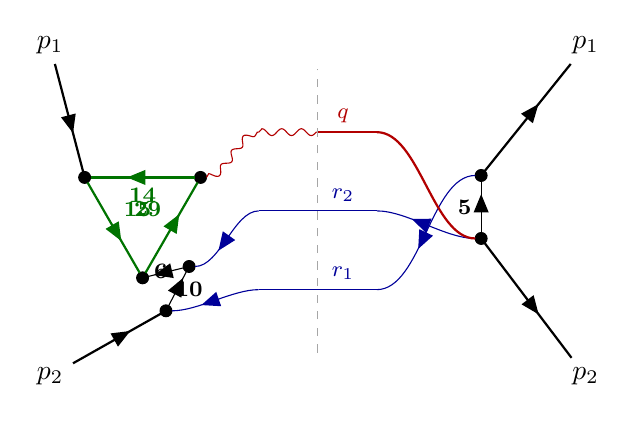
\begin{tikzpicture}
\begin{feynman}
\vertex (Lp1) at (-3.400,2.100) {$p_1$};
\vertex (Lp2) at (-3.400,-2.100) {$p_2$};
\vertex (Lcr1) at (-0.750,-1.000);
\vertex (Lcr2) at (-0.750,0.000);
\vertex (Lcq) at (-0.750,1.000);
\vertex (Mq) at (0,1.000);
\vertex[dot] (Lv0) at (-1.489,0.425) {};
\vertex[dot] (Lv1) at (-2.961,0.425) {};
\vertex[dot] (Lv2) at (-2.225,-0.850) {};
\vertex[dot] (Lt6) at (-1.928,-1.269) {};
\vertex[dot] (Lt10) at (-1.634,-0.706) {};
\vertex (Rp1) at (3.400,2.100) {$p_1$};
\vertex (Rp2) at (3.400,-2.100) {$p_2$};
\vertex (Rcr1) at (0.750,-1.000);
\vertex (Rcr2) at (0.750,0.000);
\vertex (Rcq) at (0.750,1.000);
\vertex[dot] (R5) at (2.075,0.450) {};
\vertex[dot] (Rroot) at (2.075,-0.350) {};
\diagram* {
(Lv0) -- [plain, thick, green!45!black, with arrow=0.55, edge label={\footnotesize\bfseries 14}] (Lv1),
(Lv1) -- [plain, thick, green!45!black, with arrow=0.55, edge label={\footnotesize\bfseries 15}] (Lv2),
(Lv2) -- [plain, thick, green!45!black, with arrow=0.55, edge label={\footnotesize\bfseries 29}] (Lv0),
(Lcq) -- [boson, red!70!black, out=180, in=0, looseness=0.75] (Lv0),
(Lp1) -- [plain, thick, with arrow=0.55] (Lv1),
(Lt6) -- [plain, with arrow=0.55, edge label={\footnotesize\bfseries 6}] (Lt10),
(Lt10) -- [plain, with arrow=0.55, edge label={\footnotesize\bfseries 10}] (Lv2),
(Lp2) -- [plain, thick, with arrow=0.55] (Lt6),
(Lcr1) -- [plain, blue!60!black, out=180, in=0, looseness=0.75, with arrow=0.55] (Lt6),
(Lcr2) -- [plain, blue!60!black, out=180, in=0, looseness=0.75, with arrow=0.55] (Lt10),
(Rroot) -- [plain, with arrow=0.55, edge label={\footnotesize\bfseries 5}] (R5),
(R5) -- [plain, thick, with arrow=0.55] (Rp1),
(Rroot) -- [plain, thick, with arrow=0.55] (Rp2),
(R5) -- [plain, blue!60!black, out=180, in=0, looseness=0.75, with arrow=0.55] (Rcr1),
(Rroot) -- [plain, blue!60!black, out=180, in=0, looseness=0.75, with arrow=0.55] (Rcr2),
(Rroot) -- [plain, red!70!black, double, double distance=1.2pt, thick, out=180, in=0, looseness=0.75] (Rcq),
(Rcr1) -- [plain, blue!60!black] (Lcr1),
(Rcr2) -- [plain, blue!60!black] (Lcr2),
(Rcq) -- [plain, red!70!black, double, double distance=1.2pt, thick] (Mq) -- [boson, red!70!black] (Lcq),
};
\end{feynman}
\draw[dashed, gray!70] (0,-1.80) -- (0,1.80);
\node[font=\footnotesize, blue!60!black, above] at (0.32,-1.00) {$r_1$};
\node[font=\footnotesize, blue!60!black, above] at (0.32,0.00) {$r_2$};
\node[font=\footnotesize, red!70!black, above] at (0.32,1.00) {$q$};
\end{tikzpicture}}\\[2mm]\textbf{topo5} (RR family 4, pentagon q-p1-r1-r2-p2), sector with 6 of 8 lines\\[2pt]{\footnotesize\begin{tabular}{@{}r@{\ \ }l@{\ \ }l@{}}\textbf{14} & $(k_1)^2$ & loop\\
\textbf{15} & $(k_1+p_1)^2$ & loop\\
\textbf{29} & $(k_1+p_1+p_2+r_1+r_2)^2$ & loop\\
\textbf{6} & $(p_2+r_1)^2$ & amplitude (tree on the loop)\\
\textbf{10} & $(p_2+r_1+r_2)^2$ & amplitude (tree on the loop)\\
\textbf{5} & $(p_1+r_1)^2$ & conjugate\\\end{tabular}}\\[2pt]{\scriptsize pinched: 19 = $(k_1+p_1+r_1)^2$, 27 = $(k_1+p_1+r_1+r_2)^2$}\end{minipage}

\bigskip

\begin{minipage}[t]{0.48\textwidth}\centering\resizebox{0.9\linewidth}{!}{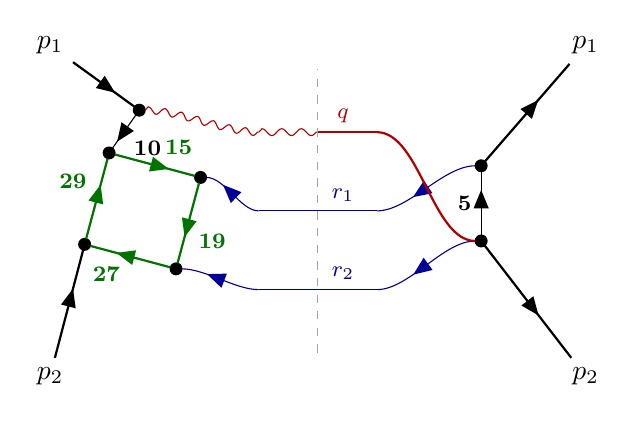
\begin{tikzpicture}
\begin{feynman}
\vertex (Lp1) at (-3.400,2.100) {$p_1$};
\vertex (Lp2) at (-3.400,-2.100) {$p_2$};
\vertex (Lcr1) at (-0.750,0.000);
\vertex (Lcr2) at (-0.750,-1.000);
\vertex (Lcq) at (-0.750,1.000);
\vertex (Mq) at (0,1.000);
\vertex[dot] (Lv0) at (-2.650,0.736) {};
\vertex[dot] (Lv1) at (-1.489,0.425) {};
\vertex[dot] (Lv2) at (-1.800,-0.736) {};
\vertex[dot] (Lv3) at (-2.961,-0.425) {};
\vertex[dot] (Lt10) at (-2.267,1.279) {};
\vertex (Rp1) at (3.400,2.100) {$p_1$};
\vertex (Rp2) at (3.400,-2.100) {$p_2$};
\vertex (Rcr1) at (0.750,0.000);
\vertex (Rcr2) at (0.750,-1.000);
\vertex (Rcq) at (0.750,1.000);
\vertex[dot] (R5) at (2.075,0.573) {};
\vertex[dot] (Rroot) at (2.075,-0.382) {};
\diagram* {
(Lv0) -- [plain, thick, green!45!black, with arrow=0.55, edge label={\footnotesize\bfseries 15}] (Lv1),
(Lv1) -- [plain, thick, green!45!black, with arrow=0.55, edge label={\footnotesize\bfseries 19}] (Lv2),
(Lv2) -- [plain, thick, green!45!black, with arrow=0.55, edge label={\footnotesize\bfseries 27}] (Lv3),
(Lv3) -- [plain, thick, green!45!black, with arrow=0.55, edge label={\footnotesize\bfseries 29}] (Lv0),
(Lt10) -- [plain, with arrow=0.55, edge label={\footnotesize\bfseries 10}] (Lv0),
(Lcq) -- [boson, red!70!black, out=180, in=0, looseness=0.75] (Lt10),
(Lp1) -- [plain, thick, with arrow=0.55] (Lt10),
(Lcr1) -- [plain, blue!60!black, out=180, in=0, looseness=0.75, with arrow=0.55] (Lv1),
(Lcr2) -- [plain, blue!60!black, out=180, in=0, looseness=0.75, with arrow=0.55] (Lv2),
(Lp2) -- [plain, thick, with arrow=0.55] (Lv3),
(Rroot) -- [plain, with arrow=0.55, edge label={\footnotesize\bfseries 5}] (R5),
(R5) -- [plain, thick, with arrow=0.55] (Rp1),
(Rroot) -- [plain, thick, with arrow=0.55] (Rp2),
(R5) -- [plain, blue!60!black, out=180, in=0, looseness=0.75, with arrow=0.55] (Rcr1),
(Rroot) -- [plain, blue!60!black, out=180, in=0, looseness=0.75, with arrow=0.55] (Rcr2),
(Rroot) -- [plain, red!70!black, double, double distance=1.2pt, thick, out=180, in=0, looseness=0.75] (Rcq),
(Rcr1) -- [plain, blue!60!black] (Lcr1),
(Rcr2) -- [plain, blue!60!black] (Lcr2),
(Rcq) -- [plain, red!70!black, double, double distance=1.2pt, thick] (Mq) -- [boson, red!70!black] (Lcq),
};
\end{feynman}
\draw[dashed, gray!70] (0,-1.80) -- (0,1.80);
\node[font=\footnotesize, blue!60!black, above] at (0.32,0.00) {$r_1$};
\node[font=\footnotesize, blue!60!black, above] at (0.32,-1.00) {$r_2$};
\node[font=\footnotesize, red!70!black, above] at (0.32,1.00) {$q$};
\end{tikzpicture}}\\[2mm]\textbf{topo5} (RR family 4, pentagon q-p1-r1-r2-p2), sector with 6 of 8 lines\\[2pt]{\footnotesize\begin{tabular}{@{}r@{\ \ }l@{\ \ }l@{}}\textbf{15} & $(k_1+p_1)^2$ & loop\\
\textbf{19} & $(k_1+p_1+r_1)^2$ & loop\\
\textbf{27} & $(k_1+p_1+r_1+r_2)^2$ & loop\\
\textbf{29} & $(k_1+p_1+p_2+r_1+r_2)^2$ & loop\\
\textbf{10} & $(p_2+r_1+r_2)^2$ & amplitude (tree on the loop)\\
\textbf{5} & $(p_1+r_1)^2$ & conjugate\\\end{tabular}}\\[2pt]{\scriptsize pinched: 6 = $(p_2+r_1)^2$, 14 = $(k_1)^2$}\end{minipage}\hfill%
\begin{minipage}[t]{0.48\textwidth}\centering\resizebox{0.9\linewidth}{!}{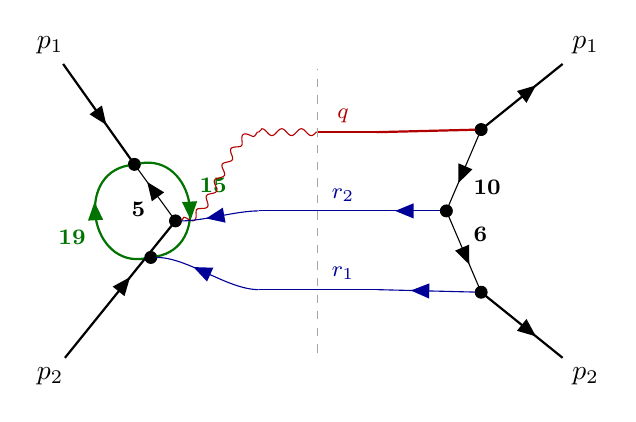
\begin{tikzpicture}
\begin{feynman}
\vertex (Lp1) at (-3.400,2.100) {$p_1$};
\vertex (Lp2) at (-3.400,-2.100) {$p_2$};
\vertex (Lcr1) at (-0.750,-1.000);
\vertex (Lcr2) at (-0.750,0.000);
\vertex (Lcq) at (-0.750,1.000);
\vertex (Mq) at (0,1.000);
\vertex[dot] (Lv0) at (-2.329,0.591) {};
\vertex[dot] (Lv1) at (-2.121,-0.591) {};
\vertex[dot] (Lt5) at (-1.807,-0.127) {};
\vertex (Rp1) at (3.400,2.100) {$p_1$};
\vertex (Rp2) at (3.400,-2.100) {$p_2$};
\vertex (Rcr1) at (0.750,-1.000);
\vertex (Rcr2) at (0.750,0.000);
\vertex (Rcq) at (0.750,1.000);
\vertex[dot] (R6) at (2.075,-1.033) {};
\vertex[dot] (R10) at (1.633,0.000) {};
\vertex[dot] (Rroot) at (2.075,1.033) {};
\diagram* {
(Lv0) -- [plain, thick, green!45!black, half left, with arrow=0.55, edge label={\footnotesize\bfseries 15}] (Lv1),
(Lv1) -- [plain, thick, green!45!black, half left, with arrow=0.55, edge label={\footnotesize\bfseries 19}] (Lv0),
(Lt5) -- [plain, with arrow=0.55, edge label={\footnotesize\bfseries 5}] (Lv0),
(Lp2) -- [plain, thick, with arrow=0.55] (Lt5),
(Lcq) -- [boson, red!70!black, out=180, in=0, looseness=0.75] (Lt5),
(Lcr2) -- [plain, blue!60!black, out=180, in=0, looseness=0.75, with arrow=0.55] (Lt5),
(Lp1) -- [plain, thick, with arrow=0.55] (Lv0),
(Lcr1) -- [plain, blue!60!black, out=180, in=0, looseness=0.75, with arrow=0.55] (Lv1),
(R10) -- [plain, with arrow=0.55, edge label={\footnotesize\bfseries 6}] (R6),
(Rroot) -- [plain, with arrow=0.55, edge label={\footnotesize\bfseries 10}] (R10),
(Rroot) -- [plain, thick, with arrow=0.55] (Rp1),
(R6) -- [plain, thick, with arrow=0.55] (Rp2),
(R6) -- [plain, blue!60!black, with arrow=0.55] (Rcr1),
(R10) -- [plain, blue!60!black, with arrow=0.55] (Rcr2),
(Rroot) -- [plain, red!70!black, double, double distance=1.2pt, thick] (Rcq),
(Rcr1) -- [plain, blue!60!black] (Lcr1),
(Rcr2) -- [plain, blue!60!black] (Lcr2),
(Rcq) -- [plain, red!70!black, double, double distance=1.2pt, thick] (Mq) -- [boson, red!70!black] (Lcq),
};
\end{feynman}
\draw[dashed, gray!70] (0,-1.80) -- (0,1.80);
\node[font=\footnotesize, blue!60!black, above] at (0.32,-1.00) {$r_1$};
\node[font=\footnotesize, blue!60!black, above] at (0.32,0.00) {$r_2$};
\node[font=\footnotesize, red!70!black, above] at (0.32,1.00) {$q$};
\end{tikzpicture}}\\[2mm]\textbf{topo5} (RR family 4, pentagon q-p1-r1-r2-p2), sector with 5 of 8 lines\\[2pt]{\footnotesize\begin{tabular}{@{}r@{\ \ }l@{\ \ }l@{}}\textbf{15} & $(k_1+p_1)^2$ & loop\\
\textbf{19} & $(k_1+p_1+r_1)^2$ & loop\\
\textbf{5} & $(p_1+r_1)^2$ & amplitude (tree on the loop)\\
\textbf{6} & $(p_2+r_1)^2$ & conjugate\\
\textbf{10} & $(p_2+r_1+r_2)^2$ & conjugate\\\end{tabular}}\\[2pt]{\scriptsize pinched: 14 = $(k_1)^2$, 27 = $(k_1+p_1+r_1+r_2)^2$, 29 = $(k_1+p_1+p_2+r_1+r_2)^2$}\end{minipage}

\bigskip

\begin{minipage}[t]{0.48\textwidth}\centering\resizebox{0.9\linewidth}{!}{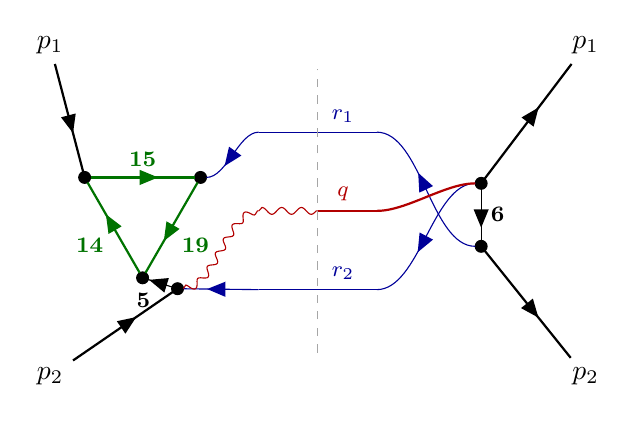
\begin{tikzpicture}
\begin{feynman}
\vertex (Lp1) at (-3.400,2.100) {$p_1$};
\vertex (Lp2) at (-3.400,-2.100) {$p_2$};
\vertex (Lcr1) at (-0.750,1.000);
\vertex (Lcr2) at (-0.750,-1.000);
\vertex (Lcq) at (-0.750,0.000);
\vertex (Mq) at (0,0.000);
\vertex[dot] (Lv0) at (-2.225,-0.850) {};
\vertex[dot] (Lv1) at (-2.961,0.425) {};
\vertex[dot] (Lv2) at (-1.489,0.425) {};
\vertex[dot] (Lt5) at (-1.781,-0.988) {};
\vertex (Rp1) at (3.400,2.100) {$p_1$};
\vertex (Rp2) at (3.400,-2.100) {$p_2$};
\vertex (Rcr1) at (0.750,1.000);
\vertex (Rcr2) at (0.750,-1.000);
\vertex (Rcq) at (0.750,0.000);
\vertex[dot] (R6) at (2.075,-0.450) {};
\vertex[dot] (Rroot) at (2.075,0.350) {};
\diagram* {
(Lv0) -- [plain, thick, green!45!black, with arrow=0.55, edge label={\footnotesize\bfseries 14}] (Lv1),
(Lv1) -- [plain, thick, green!45!black, with arrow=0.55, edge label={\footnotesize\bfseries 15}] (Lv2),
(Lv2) -- [plain, thick, green!45!black, with arrow=0.55, edge label={\footnotesize\bfseries 19}] (Lv0),
(Lt5) -- [plain, with arrow=0.55, edge label={\footnotesize\bfseries 5}] (Lv0),
(Lp2) -- [plain, thick, with arrow=0.55] (Lt5),
(Lcr2) -- [plain, blue!60!black, with arrow=0.55] (Lt5),
(Lcq) -- [boson, red!70!black, out=180, in=0, looseness=0.75] (Lt5),
(Lp1) -- [plain, thick, with arrow=0.55] (Lv1),
(Lcr1) -- [plain, blue!60!black, out=180, in=0, looseness=0.75, with arrow=0.55] (Lv2),
(Rroot) -- [plain, with arrow=0.55, edge label={\footnotesize\bfseries 6}] (R6),
(Rroot) -- [plain, thick, with arrow=0.55] (Rp1),
(R6) -- [plain, thick, with arrow=0.55] (Rp2),
(R6) -- [plain, blue!60!black, out=180, in=0, looseness=0.75, with arrow=0.55] (Rcr1),
(Rroot) -- [plain, blue!60!black, out=180, in=0, looseness=0.75, with arrow=0.55] (Rcr2),
(Rroot) -- [plain, red!70!black, double, double distance=1.2pt, thick, out=180, in=0, looseness=0.75] (Rcq),
(Rcr1) -- [plain, blue!60!black] (Lcr1),
(Rcr2) -- [plain, blue!60!black] (Lcr2),
(Rcq) -- [plain, red!70!black, double, double distance=1.2pt, thick] (Mq) -- [boson, red!70!black] (Lcq),
};
\end{feynman}
\draw[dashed, gray!70] (0,-1.80) -- (0,1.80);
\node[font=\footnotesize, blue!60!black, above] at (0.32,1.00) {$r_1$};
\node[font=\footnotesize, blue!60!black, above] at (0.32,-1.00) {$r_2$};
\node[font=\footnotesize, red!70!black, above] at (0.32,0.00) {$q$};
\end{tikzpicture}}\\[2mm]\textbf{topo5} (RR family 4, pentagon q-p1-r1-r2-p2), sector with 5 of 8 lines\\[2pt]{\footnotesize\begin{tabular}{@{}r@{\ \ }l@{\ \ }l@{}}\textbf{14} & $(k_1)^2$ & loop\\
\textbf{15} & $(k_1+p_1)^2$ & loop\\
\textbf{19} & $(k_1+p_1+r_1)^2$ & loop\\
\textbf{5} & $(p_1+r_1)^2$ & amplitude (tree on the loop)\\
\textbf{6} & $(p_2+r_1)^2$ & conjugate\\\end{tabular}}\\[2pt]{\scriptsize pinched: 10 = $(p_2+r_1+r_2)^2$, 27 = $(k_1+p_1+r_1+r_2)^2$, 29 = $(k_1+p_1+p_2+r_1+r_2)^2$}\end{minipage}\hfill%
\begin{minipage}[t]{0.48\textwidth}\centering\resizebox{0.9\linewidth}{!}{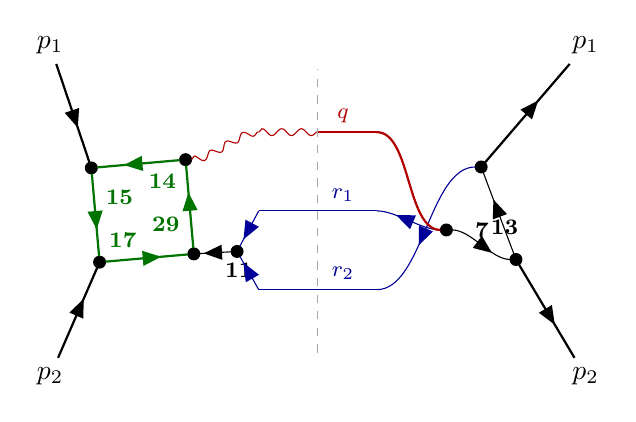
\begin{tikzpicture}
\begin{feynman}
\vertex (Lp1) at (-3.400,2.100) {$p_1$};
\vertex (Lp2) at (-3.400,-2.100) {$p_2$};
\vertex (Lcr1) at (-0.750,0.000);
\vertex (Lcr2) at (-0.750,-1.000);
\vertex (Lcq) at (-0.750,1.000);
\vertex (Mq) at (0,1.000);
\vertex[dot] (Lv0) at (-1.679,0.651) {};
\vertex[dot] (Lv1) at (-2.876,0.546) {};
\vertex[dot] (Lv2) at (-2.771,-0.651) {};
\vertex[dot] (Lv3) at (-1.574,-0.546) {};
\vertex[dot] (Lt11) at (-1.025,-0.515) {};
\vertex (Rp1) at (3.400,2.100) {$p_1$};
\vertex (Rp2) at (3.400,-2.100) {$p_2$};
\vertex (Rcr1) at (0.750,0.000);
\vertex (Rcr2) at (0.750,-1.000);
\vertex (Rcq) at (0.750,1.000);
\vertex[dot] (R7) at (2.075,0.558) {};
\vertex[dot] (R13) at (2.517,-0.617) {};
\vertex[dot] (Rroot) at (1.633,-0.242) {};
\diagram* {
(Lv0) -- [plain, thick, green!45!black, with arrow=0.55, edge label={\footnotesize\bfseries 14}] (Lv1),
(Lv1) -- [plain, thick, green!45!black, with arrow=0.55, edge label={\footnotesize\bfseries 15}] (Lv2),
(Lv2) -- [plain, thick, green!45!black, with arrow=0.55, edge label={\footnotesize\bfseries 17}] (Lv3),
(Lv3) -- [plain, thick, green!45!black, with arrow=0.55, edge label={\footnotesize\bfseries 29}] (Lv0),
(Lcq) -- [boson, red!70!black, out=180, in=0, looseness=0.75] (Lv0),
(Lp1) -- [plain, thick, with arrow=0.55] (Lv1),
(Lp2) -- [plain, thick, with arrow=0.55] (Lv2),
(Lt11) -- [plain, with arrow=0.55, edge label={\footnotesize\bfseries 11}] (Lv3),
(Lcr1) -- [plain, blue!60!black, with arrow=0.55] (Lt11),
(Lcr2) -- [plain, blue!60!black, with arrow=0.55] (Lt11),
(R13) -- [plain, with arrow=0.55, edge label={\footnotesize\bfseries 7}] (R7),
(Rroot) -- [plain, out=0, in=180, looseness=0.75, with arrow=0.55, edge label={\footnotesize\bfseries 13}] (R13),
(R7) -- [plain, thick, with arrow=0.55] (Rp1),
(R13) -- [plain, thick, with arrow=0.55] (Rp2),
(Rroot) -- [plain, blue!60!black, out=180, in=0, looseness=0.75, with arrow=0.55] (Rcr1),
(R7) -- [plain, blue!60!black, out=180, in=0, looseness=0.75, with arrow=0.55] (Rcr2),
(Rroot) -- [plain, red!70!black, double, double distance=1.2pt, thick, out=180, in=0, looseness=0.75] (Rcq),
(Rcr1) -- [plain, blue!60!black] (Lcr1),
(Rcr2) -- [plain, blue!60!black] (Lcr2),
(Rcq) -- [plain, red!70!black, double, double distance=1.2pt, thick] (Mq) -- [boson, red!70!black] (Lcq),
};
\end{feynman}
\draw[dashed, gray!70] (0,-1.80) -- (0,1.80);
\node[font=\footnotesize, blue!60!black, above] at (0.32,0.00) {$r_1$};
\node[font=\footnotesize, blue!60!black, above] at (0.32,-1.00) {$r_2$};
\node[font=\footnotesize, red!70!black, above] at (0.32,1.00) {$q$};
\end{tikzpicture}}\\[2mm]\textbf{topo6} (RR family 30, pentagon q-p1-p2-r2-r1), sector with 7 of 8 lines\\[2pt]{\footnotesize\begin{tabular}{@{}r@{\ \ }l@{\ \ }l@{}}\textbf{14} & $(k_1)^2$ & loop\\
\textbf{15} & $(k_1+p_1)^2$ & loop\\
\textbf{17} & $(k_1+p_1+p_2)^2$ & loop\\
\textbf{29} & $(k_1+p_1+p_2+r_1+r_2)^2$ & loop\\
\textbf{11} & $(r_1+r_2)^2$ & amplitude (tree on the loop)\\
\textbf{7} & $(p_1+r_2)^2$ & conjugate\\
\textbf{13} & $(p_1+p_2+r_2)^2$ & conjugate\\\end{tabular}}\\[2pt]{\scriptsize pinched: 25 = $(k_1+p_1+p_2+r_2)^2$}\end{minipage}

\bigskip

\begin{minipage}[t]{0.48\textwidth}\centering\resizebox{0.9\linewidth}{!}{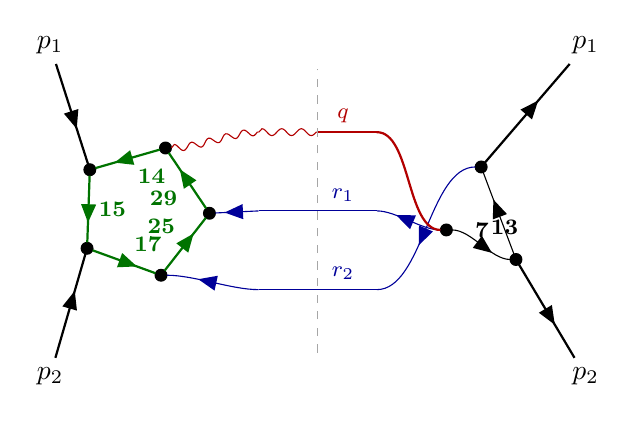
\begin{tikzpicture}
\begin{feynman}
\vertex (Lp1) at (-3.400,2.100) {$p_1$};
\vertex (Lp2) at (-3.400,-2.100) {$p_2$};
\vertex (Lcr1) at (-0.750,0.000);
\vertex (Lcr2) at (-0.750,-1.000);
\vertex (Lcq) at (-0.750,1.000);
\vertex (Mq) at (0,1.000);
\vertex[dot] (Lv0) at (-1.934,0.799) {};
\vertex[dot] (Lv1) at (-2.895,0.523) {};
\vertex[dot] (Lv2) at (-2.930,-0.475) {};
\vertex[dot] (Lv3) at (-1.991,-0.817) {};
\vertex[dot] (Lv4) at (-1.376,-0.030) {};
\vertex (Rp1) at (3.400,2.100) {$p_1$};
\vertex (Rp2) at (3.400,-2.100) {$p_2$};
\vertex (Rcr1) at (0.750,0.000);
\vertex (Rcr2) at (0.750,-1.000);
\vertex (Rcq) at (0.750,1.000);
\vertex[dot] (R7) at (2.075,0.558) {};
\vertex[dot] (R13) at (2.517,-0.617) {};
\vertex[dot] (Rroot) at (1.633,-0.242) {};
\diagram* {
(Lv0) -- [plain, thick, green!45!black, with arrow=0.55, edge label={\footnotesize\bfseries 14}] (Lv1),
(Lv1) -- [plain, thick, green!45!black, with arrow=0.55, edge label={\footnotesize\bfseries 15}] (Lv2),
(Lv2) -- [plain, thick, green!45!black, with arrow=0.55, edge label={\footnotesize\bfseries 17}] (Lv3),
(Lv3) -- [plain, thick, green!45!black, with arrow=0.55, edge label={\footnotesize\bfseries 25}] (Lv4),
(Lv4) -- [plain, thick, green!45!black, with arrow=0.55, edge label={\footnotesize\bfseries 29}] (Lv0),
(Lcq) -- [boson, red!70!black, out=180, in=0, looseness=0.75] (Lv0),
(Lp1) -- [plain, thick, with arrow=0.55] (Lv1),
(Lp2) -- [plain, thick, with arrow=0.55] (Lv2),
(Lcr2) -- [plain, blue!60!black, out=180, in=0, looseness=0.75, with arrow=0.55] (Lv3),
(Lcr1) -- [plain, blue!60!black, with arrow=0.55] (Lv4),
(R13) -- [plain, with arrow=0.55, edge label={\footnotesize\bfseries 7}] (R7),
(Rroot) -- [plain, out=0, in=180, looseness=0.75, with arrow=0.55, edge label={\footnotesize\bfseries 13}] (R13),
(R7) -- [plain, thick, with arrow=0.55] (Rp1),
(R13) -- [plain, thick, with arrow=0.55] (Rp2),
(Rroot) -- [plain, blue!60!black, out=180, in=0, looseness=0.75, with arrow=0.55] (Rcr1),
(R7) -- [plain, blue!60!black, out=180, in=0, looseness=0.75, with arrow=0.55] (Rcr2),
(Rroot) -- [plain, red!70!black, double, double distance=1.2pt, thick, out=180, in=0, looseness=0.75] (Rcq),
(Rcr1) -- [plain, blue!60!black] (Lcr1),
(Rcr2) -- [plain, blue!60!black] (Lcr2),
(Rcq) -- [plain, red!70!black, double, double distance=1.2pt, thick] (Mq) -- [boson, red!70!black] (Lcq),
};
\end{feynman}
\draw[dashed, gray!70] (0,-1.80) -- (0,1.80);
\node[font=\footnotesize, blue!60!black, above] at (0.32,0.00) {$r_1$};
\node[font=\footnotesize, blue!60!black, above] at (0.32,-1.00) {$r_2$};
\node[font=\footnotesize, red!70!black, above] at (0.32,1.00) {$q$};
\end{tikzpicture}}\\[2mm]\textbf{topo6} (RR family 30, pentagon q-p1-p2-r2-r1), sector with 7 of 8 lines\\[2pt]{\footnotesize\begin{tabular}{@{}r@{\ \ }l@{\ \ }l@{}}\textbf{14} & $(k_1)^2$ & loop\\
\textbf{15} & $(k_1+p_1)^2$ & loop\\
\textbf{17} & $(k_1+p_1+p_2)^2$ & loop\\
\textbf{25} & $(k_1+p_1+p_2+r_2)^2$ & loop\\
\textbf{29} & $(k_1+p_1+p_2+r_1+r_2)^2$ & loop\\
\textbf{7} & $(p_1+r_2)^2$ & conjugate\\
\textbf{13} & $(p_1+p_2+r_2)^2$ & conjugate\\\end{tabular}}\\[2pt]{\scriptsize pinched: 11 = $(r_1+r_2)^2$}\end{minipage}\hfill%
\begin{minipage}[t]{0.48\textwidth}\centering\resizebox{0.9\linewidth}{!}{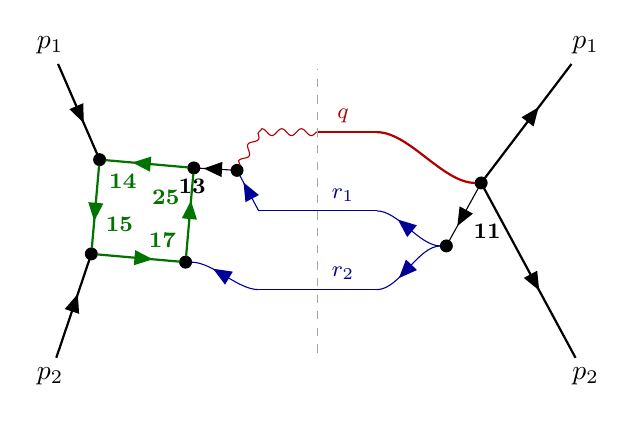
\begin{tikzpicture}
\begin{feynman}
\vertex (Lp1) at (-3.400,2.100) {$p_1$};
\vertex (Lp2) at (-3.400,-2.100) {$p_2$};
\vertex (Lcr1) at (-0.750,0.000);
\vertex (Lcr2) at (-0.750,-1.000);
\vertex (Lcq) at (-0.750,1.000);
\vertex (Mq) at (0,1.000);
\vertex[dot] (Lv0) at (-1.574,0.546) {};
\vertex[dot] (Lv1) at (-2.771,0.651) {};
\vertex[dot] (Lv2) at (-2.876,-0.546) {};
\vertex[dot] (Lv3) at (-1.679,-0.651) {};
\vertex[dot] (Lt13) at (-1.025,0.515) {};
\vertex (Rp1) at (3.400,2.100) {$p_1$};
\vertex (Rp2) at (3.400,-2.100) {$p_2$};
\vertex (Rcr1) at (0.750,0.000);
\vertex (Rcr2) at (0.750,-1.000);
\vertex (Rcq) at (0.750,1.000);
\vertex[dot] (R11) at (1.633,-0.445) {};
\vertex[dot] (Rroot) at (2.075,0.355) {};
\diagram* {
(Lv0) -- [plain, thick, green!45!black, with arrow=0.55, edge label={\footnotesize\bfseries 14}] (Lv1),
(Lv1) -- [plain, thick, green!45!black, with arrow=0.55, edge label={\footnotesize\bfseries 15}] (Lv2),
(Lv2) -- [plain, thick, green!45!black, with arrow=0.55, edge label={\footnotesize\bfseries 17}] (Lv3),
(Lv3) -- [plain, thick, green!45!black, with arrow=0.55, edge label={\footnotesize\bfseries 25}] (Lv0),
(Lt13) -- [plain, with arrow=0.55, edge label={\footnotesize\bfseries 13}] (Lv0),
(Lcr1) -- [plain, blue!60!black, with arrow=0.55] (Lt13),
(Lcq) -- [boson, red!70!black] (Lt13),
(Lp1) -- [plain, thick, with arrow=0.55] (Lv1),
(Lp2) -- [plain, thick, with arrow=0.55] (Lv2),
(Lcr2) -- [plain, blue!60!black, out=180, in=0, looseness=0.75, with arrow=0.55] (Lv3),
(Rroot) -- [plain, with arrow=0.55, edge label={\footnotesize\bfseries 11}] (R11),
(Rroot) -- [plain, thick, with arrow=0.55] (Rp1),
(Rroot) -- [plain, thick, with arrow=0.55] (Rp2),
(R11) -- [plain, blue!60!black, out=180, in=0, looseness=0.75, with arrow=0.55] (Rcr1),
(R11) -- [plain, blue!60!black, out=180, in=0, looseness=0.75, with arrow=0.55] (Rcr2),
(Rroot) -- [plain, red!70!black, double, double distance=1.2pt, thick, out=180, in=0, looseness=0.75] (Rcq),
(Rcr1) -- [plain, blue!60!black] (Lcr1),
(Rcr2) -- [plain, blue!60!black] (Lcr2),
(Rcq) -- [plain, red!70!black, double, double distance=1.2pt, thick] (Mq) -- [boson, red!70!black] (Lcq),
};
\end{feynman}
\draw[dashed, gray!70] (0,-1.80) -- (0,1.80);
\node[font=\footnotesize, blue!60!black, above] at (0.32,0.00) {$r_1$};
\node[font=\footnotesize, blue!60!black, above] at (0.32,-1.00) {$r_2$};
\node[font=\footnotesize, red!70!black, above] at (0.32,1.00) {$q$};
\end{tikzpicture}}\\[2mm]\textbf{topo6} (RR family 30, pentagon q-p1-p2-r2-r1), sector with 6 of 8 lines\\[2pt]{\footnotesize\begin{tabular}{@{}r@{\ \ }l@{\ \ }l@{}}\textbf{14} & $(k_1)^2$ & loop\\
\textbf{15} & $(k_1+p_1)^2$ & loop\\
\textbf{17} & $(k_1+p_1+p_2)^2$ & loop\\
\textbf{25} & $(k_1+p_1+p_2+r_2)^2$ & loop\\
\textbf{13} & $(p_1+p_2+r_2)^2$ & amplitude (tree on the loop)\\
\textbf{11} & $(r_1+r_2)^2$ & conjugate\\\end{tabular}}\\[2pt]{\scriptsize pinched: 7 = $(p_1+r_2)^2$, 29 = $(k_1+p_1+p_2+r_1+r_2)^2$}\end{minipage}

\bigskip

\begin{minipage}[t]{0.48\textwidth}\centering\resizebox{0.9\linewidth}{!}{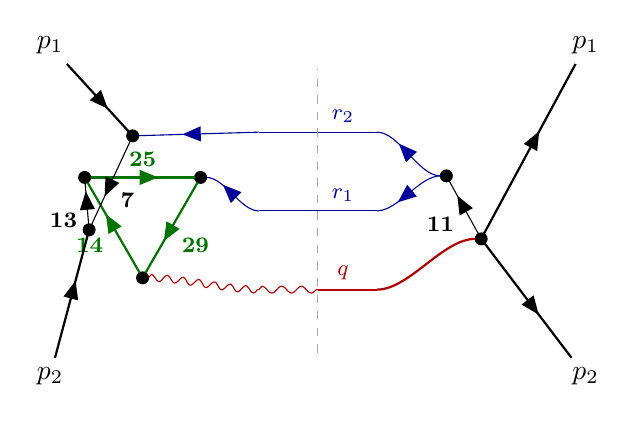
\begin{tikzpicture}
\begin{feynman}
\vertex (Lp1) at (-3.400,2.100) {$p_1$};
\vertex (Lp2) at (-3.400,-2.100) {$p_2$};
\vertex (Lcr1) at (-0.750,0.000);
\vertex (Lcr2) at (-0.750,1.000);
\vertex (Lcq) at (-0.750,-1.000);
\vertex (Mq) at (0,-1.000);
\vertex[dot] (Lv0) at (-2.225,-0.850) {};
\vertex[dot] (Lv1) at (-2.961,0.425) {};
\vertex[dot] (Lv2) at (-1.489,0.425) {};
\vertex[dot] (Lt7) at (-2.351,0.953) {};
\vertex[dot] (Lt13) at (-2.904,-0.241) {};
\vertex (Rp1) at (3.400,2.100) {$p_1$};
\vertex (Rp2) at (3.400,-2.100) {$p_2$};
\vertex (Rcr1) at (0.750,0.000);
\vertex (Rcr2) at (0.750,1.000);
\vertex (Rcq) at (0.750,-1.000);
\vertex[dot] (R11) at (1.633,0.445) {};
\vertex[dot] (Rroot) at (2.075,-0.355) {};
\diagram* {
(Lv0) -- [plain, thick, green!45!black, with arrow=0.55, edge label={\footnotesize\bfseries 14}] (Lv1),
(Lv1) -- [plain, thick, green!45!black, with arrow=0.55, edge label={\footnotesize\bfseries 25}] (Lv2),
(Lv2) -- [plain, thick, green!45!black, with arrow=0.55, edge label={\footnotesize\bfseries 29}] (Lv0),
(Lcq) -- [boson, red!70!black, out=180, in=0, looseness=0.75] (Lv0),
(Lt7) -- [plain, with arrow=0.55, edge label={\footnotesize\bfseries 7}] (Lt13),
(Lt13) -- [plain, with arrow=0.55, edge label={\footnotesize\bfseries 13}] (Lv1),
(Lp2) -- [plain, thick, with arrow=0.55] (Lt13),
(Lcr2) -- [plain, blue!60!black, with arrow=0.55] (Lt7),
(Lp1) -- [plain, thick, with arrow=0.55] (Lt7),
(Lcr1) -- [plain, blue!60!black, out=180, in=0, looseness=0.75, with arrow=0.55] (Lv2),
(Rroot) -- [plain, with arrow=0.55, edge label={\footnotesize\bfseries 11}] (R11),
(Rroot) -- [plain, thick, with arrow=0.55] (Rp1),
(Rroot) -- [plain, thick, with arrow=0.55] (Rp2),
(R11) -- [plain, blue!60!black, out=180, in=0, looseness=0.75, with arrow=0.55] (Rcr1),
(R11) -- [plain, blue!60!black, out=180, in=0, looseness=0.75, with arrow=0.55] (Rcr2),
(Rroot) -- [plain, red!70!black, double, double distance=1.2pt, thick, out=180, in=0, looseness=0.75] (Rcq),
(Rcr1) -- [plain, blue!60!black] (Lcr1),
(Rcr2) -- [plain, blue!60!black] (Lcr2),
(Rcq) -- [plain, red!70!black, double, double distance=1.2pt, thick] (Mq) -- [boson, red!70!black] (Lcq),
};
\end{feynman}
\draw[dashed, gray!70] (0,-1.80) -- (0,1.80);
\node[font=\footnotesize, blue!60!black, above] at (0.32,0.00) {$r_1$};
\node[font=\footnotesize, blue!60!black, above] at (0.32,1.00) {$r_2$};
\node[font=\footnotesize, red!70!black, above] at (0.32,-1.00) {$q$};
\end{tikzpicture}}\\[2mm]\textbf{topo6} (RR family 30, pentagon q-p1-p2-r2-r1), sector with 6 of 8 lines\\[2pt]{\footnotesize\begin{tabular}{@{}r@{\ \ }l@{\ \ }l@{}}\textbf{14} & $(k_1)^2$ & loop\\
\textbf{25} & $(k_1+p_1+p_2+r_2)^2$ & loop\\
\textbf{29} & $(k_1+p_1+p_2+r_1+r_2)^2$ & loop\\
\textbf{7} & $(p_1+r_2)^2$ & amplitude (tree on the loop)\\
\textbf{13} & $(p_1+p_2+r_2)^2$ & amplitude (tree on the loop)\\
\textbf{11} & $(r_1+r_2)^2$ & conjugate\\\end{tabular}}\\[2pt]{\scriptsize pinched: 15 = $(k_1+p_1)^2$, 17 = $(k_1+p_1+p_2)^2$}\end{minipage}\hfill%
\begin{minipage}[t]{0.48\textwidth}\centering\resizebox{0.9\linewidth}{!}{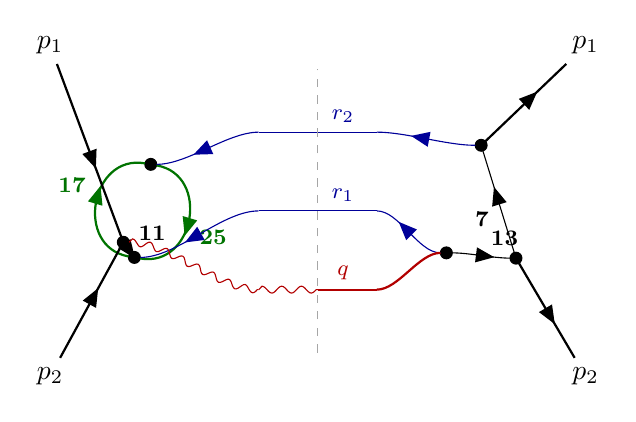
\begin{tikzpicture}
\begin{feynman}
\vertex (Lp1) at (-3.400,2.100) {$p_1$};
\vertex (Lp2) at (-3.400,-2.100) {$p_2$};
\vertex (Lcr1) at (-0.750,0.000);
\vertex (Lcr2) at (-0.750,1.000);
\vertex (Lcq) at (-0.750,-1.000);
\vertex (Mq) at (0,-1.000);
\vertex[dot] (Lv0) at (-2.329,-0.591) {};
\vertex[dot] (Lv1) at (-2.121,0.591) {};
\vertex[dot] (Lt11) at (-2.470,-0.398) {};
\vertex (Rp1) at (3.400,2.100) {$p_1$};
\vertex (Rp2) at (3.400,-2.100) {$p_2$};
\vertex (Rcr1) at (0.750,0.000);
\vertex (Rcr2) at (0.750,1.000);
\vertex (Rcq) at (0.750,-1.000);
\vertex[dot] (R7) at (2.075,0.833) {};
\vertex[dot] (R13) at (2.517,-0.600) {};
\vertex[dot] (Rroot) at (1.633,-0.533) {};
\diagram* {
(Lv0) -- [plain, thick, green!45!black, half left, with arrow=0.55, edge label={\footnotesize\bfseries 17}] (Lv1),
(Lv1) -- [plain, thick, green!45!black, half left, with arrow=0.55, edge label={\footnotesize\bfseries 25}] (Lv0),
(Lt11) -- [plain, with arrow=0.55, edge label={\footnotesize\bfseries 11}] (Lv0),
(Lp2) -- [plain, thick, with arrow=0.55] (Lt11),
(Lcr1) -- [plain, blue!60!black, out=180, in=0, looseness=0.75, with arrow=0.55] (Lv0),
(Lcq) -- [boson, red!70!black, out=180, in=0, looseness=0.75] (Lt11),
(Lp1) -- [plain, thick, with arrow=0.55] (Lt11),
(Lcr2) -- [plain, blue!60!black, out=180, in=0, looseness=0.75, with arrow=0.55] (Lv1),
(R13) -- [plain, with arrow=0.55, edge label={\footnotesize\bfseries 7}] (R7),
(Rroot) -- [plain, out=0, in=180, looseness=0.75, with arrow=0.55, edge label={\footnotesize\bfseries 13}] (R13),
(R7) -- [plain, thick, with arrow=0.55] (Rp1),
(R13) -- [plain, thick, with arrow=0.55] (Rp2),
(Rroot) -- [plain, blue!60!black, out=180, in=0, looseness=0.75, with arrow=0.55] (Rcr1),
(R7) -- [plain, blue!60!black, out=180, in=0, looseness=0.75, with arrow=0.55] (Rcr2),
(Rroot) -- [plain, red!70!black, double, double distance=1.2pt, thick, out=180, in=0, looseness=0.75] (Rcq),
(Rcr1) -- [plain, blue!60!black] (Lcr1),
(Rcr2) -- [plain, blue!60!black] (Lcr2),
(Rcq) -- [plain, red!70!black, double, double distance=1.2pt, thick] (Mq) -- [boson, red!70!black] (Lcq),
};
\end{feynman}
\draw[dashed, gray!70] (0,-1.80) -- (0,1.80);
\node[font=\footnotesize, blue!60!black, above] at (0.32,0.00) {$r_1$};
\node[font=\footnotesize, blue!60!black, above] at (0.32,1.00) {$r_2$};
\node[font=\footnotesize, red!70!black, above] at (0.32,-1.00) {$q$};
\end{tikzpicture}}\\[2mm]\textbf{topo6} (RR family 30, pentagon q-p1-p2-r2-r1), sector with 5 of 8 lines\\[2pt]{\footnotesize\begin{tabular}{@{}r@{\ \ }l@{\ \ }l@{}}\textbf{17} & $(k_1+p_1+p_2)^2$ & loop\\
\textbf{25} & $(k_1+p_1+p_2+r_2)^2$ & loop\\
\textbf{11} & $(r_1+r_2)^2$ & amplitude (tree on the loop)\\
\textbf{7} & $(p_1+r_2)^2$ & conjugate\\
\textbf{13} & $(p_1+p_2+r_2)^2$ & conjugate\\\end{tabular}}\\[2pt]{\scriptsize pinched: 14 = $(k_1)^2$, 15 = $(k_1+p_1)^2$, 29 = $(k_1+p_1+p_2+r_1+r_2)^2$}\end{minipage}

\bigskip

\begin{minipage}[t]{0.48\textwidth}\centering\resizebox{0.9\linewidth}{!}{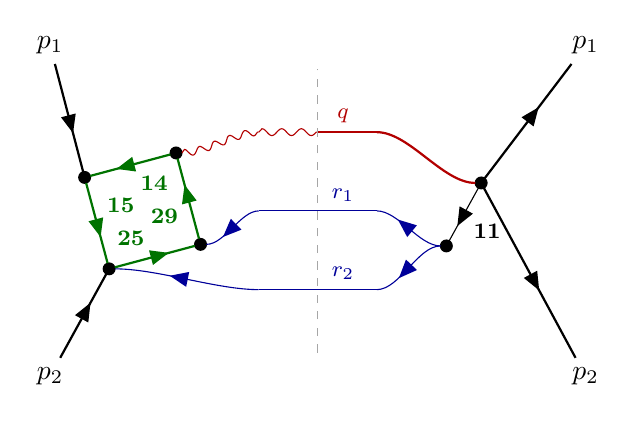
\begin{tikzpicture}
\begin{feynman}
\vertex (Lp1) at (-3.400,2.100) {$p_1$};
\vertex (Lp2) at (-3.400,-2.100) {$p_2$};
\vertex (Lcr1) at (-0.750,0.000);
\vertex (Lcr2) at (-0.750,-1.000);
\vertex (Lcq) at (-0.750,1.000);
\vertex (Mq) at (0,1.000);
\vertex[dot] (Lv0) at (-1.800,0.736) {};
\vertex[dot] (Lv1) at (-2.961,0.425) {};
\vertex[dot] (Lv2) at (-2.650,-0.736) {};
\vertex[dot] (Lv3) at (-1.489,-0.425) {};
\vertex (Rp1) at (3.400,2.100) {$p_1$};
\vertex (Rp2) at (3.400,-2.100) {$p_2$};
\vertex (Rcr1) at (0.750,0.000);
\vertex (Rcr2) at (0.750,-1.000);
\vertex (Rcq) at (0.750,1.000);
\vertex[dot] (R11) at (1.633,-0.445) {};
\vertex[dot] (Rroot) at (2.075,0.355) {};
\diagram* {
(Lv0) -- [plain, thick, green!45!black, with arrow=0.55, edge label={\footnotesize\bfseries 14}] (Lv1),
(Lv1) -- [plain, thick, green!45!black, with arrow=0.55, edge label={\footnotesize\bfseries 15}] (Lv2),
(Lv2) -- [plain, thick, green!45!black, with arrow=0.55, edge label={\footnotesize\bfseries 25}] (Lv3),
(Lv3) -- [plain, thick, green!45!black, with arrow=0.55, edge label={\footnotesize\bfseries 29}] (Lv0),
(Lcq) -- [boson, red!70!black, out=180, in=0, looseness=0.75] (Lv0),
(Lp1) -- [plain, thick, with arrow=0.55] (Lv1),
(Lp2) -- [plain, thick, with arrow=0.55] (Lv2),
(Lcr2) -- [plain, blue!60!black, out=180, in=0, looseness=0.75, with arrow=0.55] (Lv2),
(Lcr1) -- [plain, blue!60!black, out=180, in=0, looseness=0.75, with arrow=0.55] (Lv3),
(Rroot) -- [plain, with arrow=0.55, edge label={\footnotesize\bfseries 11}] (R11),
(Rroot) -- [plain, thick, with arrow=0.55] (Rp1),
(Rroot) -- [plain, thick, with arrow=0.55] (Rp2),
(R11) -- [plain, blue!60!black, out=180, in=0, looseness=0.75, with arrow=0.55] (Rcr1),
(R11) -- [plain, blue!60!black, out=180, in=0, looseness=0.75, with arrow=0.55] (Rcr2),
(Rroot) -- [plain, red!70!black, double, double distance=1.2pt, thick, out=180, in=0, looseness=0.75] (Rcq),
(Rcr1) -- [plain, blue!60!black] (Lcr1),
(Rcr2) -- [plain, blue!60!black] (Lcr2),
(Rcq) -- [plain, red!70!black, double, double distance=1.2pt, thick] (Mq) -- [boson, red!70!black] (Lcq),
};
\end{feynman}
\draw[dashed, gray!70] (0,-1.80) -- (0,1.80);
\node[font=\footnotesize, blue!60!black, above] at (0.32,0.00) {$r_1$};
\node[font=\footnotesize, blue!60!black, above] at (0.32,-1.00) {$r_2$};
\node[font=\footnotesize, red!70!black, above] at (0.32,1.00) {$q$};
\end{tikzpicture}}\\[2mm]\textbf{topo6} (RR family 30, pentagon q-p1-p2-r2-r1), sector with 5 of 8 lines\\[2pt]{\footnotesize\begin{tabular}{@{}r@{\ \ }l@{\ \ }l@{}}\textbf{14} & $(k_1)^2$ & loop\\
\textbf{15} & $(k_1+p_1)^2$ & loop\\
\textbf{25} & $(k_1+p_1+p_2+r_2)^2$ & loop\\
\textbf{29} & $(k_1+p_1+p_2+r_1+r_2)^2$ & loop\\
\textbf{11} & $(r_1+r_2)^2$ & conjugate\\\end{tabular}}\\[2pt]{\scriptsize pinched: 7 = $(p_1+r_2)^2$, 13 = $(p_1+p_2+r_2)^2$, 17 = $(k_1+p_1+p_2)^2$}\end{minipage}\hfill%
\begin{minipage}[t]{0.48\textwidth}\centering\resizebox{0.9\linewidth}{!}{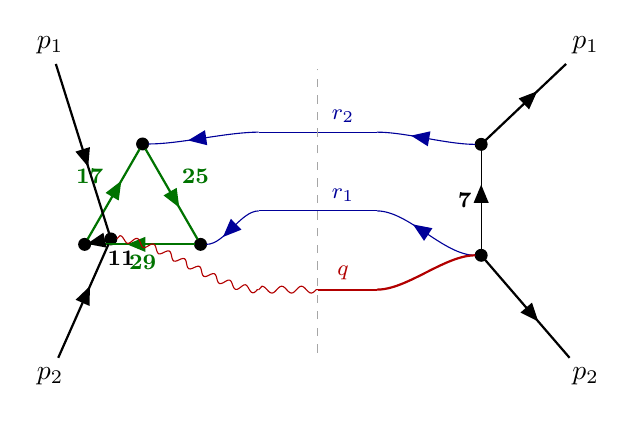
\begin{tikzpicture}
\begin{feynman}
\vertex (Lp1) at (-3.400,2.100) {$p_1$};
\vertex (Lp2) at (-3.400,-2.100) {$p_2$};
\vertex (Lcr1) at (-0.750,0.000);
\vertex (Lcr2) at (-0.750,1.000);
\vertex (Lcq) at (-0.750,-1.000);
\vertex (Mq) at (0,-1.000);
\vertex[dot] (Lv0) at (-2.961,-0.425) {};
\vertex[dot] (Lv1) at (-2.225,0.850) {};
\vertex[dot] (Lv2) at (-1.489,-0.425) {};
\vertex[dot] (Lt11) at (-2.628,-0.356) {};
\vertex (Rp1) at (3.400,2.100) {$p_1$};
\vertex (Rp2) at (3.400,-2.100) {$p_2$};
\vertex (Rcr1) at (0.750,0.000);
\vertex (Rcr2) at (0.750,1.000);
\vertex (Rcq) at (0.750,-1.000);
\vertex[dot] (R7) at (2.075,0.845) {};
\vertex[dot] (Rroot) at (2.075,-0.564) {};
\diagram* {
(Lv0) -- [plain, thick, green!45!black, with arrow=0.55, edge label={\footnotesize\bfseries 17}] (Lv1),
(Lv1) -- [plain, thick, green!45!black, with arrow=0.55, edge label={\footnotesize\bfseries 25}] (Lv2),
(Lv2) -- [plain, thick, green!45!black, with arrow=0.55, edge label={\footnotesize\bfseries 29}] (Lv0),
(Lt11) -- [plain, with arrow=0.55, edge label={\footnotesize\bfseries 11}] (Lv0),
(Lp2) -- [plain, thick, with arrow=0.55] (Lt11),
(Lcq) -- [boson, red!70!black, out=180, in=0, looseness=0.75] (Lt11),
(Lp1) -- [plain, thick, with arrow=0.55] (Lt11),
(Lcr2) -- [plain, blue!60!black, out=180, in=0, looseness=0.75, with arrow=0.55] (Lv1),
(Lcr1) -- [plain, blue!60!black, out=180, in=0, looseness=0.75, with arrow=0.55] (Lv2),
(Rroot) -- [plain, with arrow=0.55, edge label={\footnotesize\bfseries 7}] (R7),
(R7) -- [plain, thick, with arrow=0.55] (Rp1),
(Rroot) -- [plain, thick, with arrow=0.55] (Rp2),
(Rroot) -- [plain, blue!60!black, out=180, in=0, looseness=0.75, with arrow=0.55] (Rcr1),
(R7) -- [plain, blue!60!black, out=180, in=0, looseness=0.75, with arrow=0.55] (Rcr2),
(Rroot) -- [plain, red!70!black, double, double distance=1.2pt, thick, out=180, in=0, looseness=0.75] (Rcq),
(Rcr1) -- [plain, blue!60!black] (Lcr1),
(Rcr2) -- [plain, blue!60!black] (Lcr2),
(Rcq) -- [plain, red!70!black, double, double distance=1.2pt, thick] (Mq) -- [boson, red!70!black] (Lcq),
};
\end{feynman}
\draw[dashed, gray!70] (0,-1.80) -- (0,1.80);
\node[font=\footnotesize, blue!60!black, above] at (0.32,0.00) {$r_1$};
\node[font=\footnotesize, blue!60!black, above] at (0.32,1.00) {$r_2$};
\node[font=\footnotesize, red!70!black, above] at (0.32,-1.00) {$q$};
\end{tikzpicture}}\\[2mm]\textbf{topo6} (RR family 30, pentagon q-p1-p2-r2-r1), sector with 5 of 8 lines\\[2pt]{\footnotesize\begin{tabular}{@{}r@{\ \ }l@{\ \ }l@{}}\textbf{17} & $(k_1+p_1+p_2)^2$ & loop\\
\textbf{25} & $(k_1+p_1+p_2+r_2)^2$ & loop\\
\textbf{29} & $(k_1+p_1+p_2+r_1+r_2)^2$ & loop\\
\textbf{11} & $(r_1+r_2)^2$ & amplitude (tree on the loop)\\
\textbf{7} & $(p_1+r_2)^2$ & conjugate\\\end{tabular}}\\[2pt]{\scriptsize pinched: 13 = $(p_1+p_2+r_2)^2$, 14 = $(k_1)^2$, 15 = $(k_1+p_1)^2$}\end{minipage}

\bigskip

\begin{minipage}[t]{0.48\textwidth}\centering\resizebox{0.9\linewidth}{!}{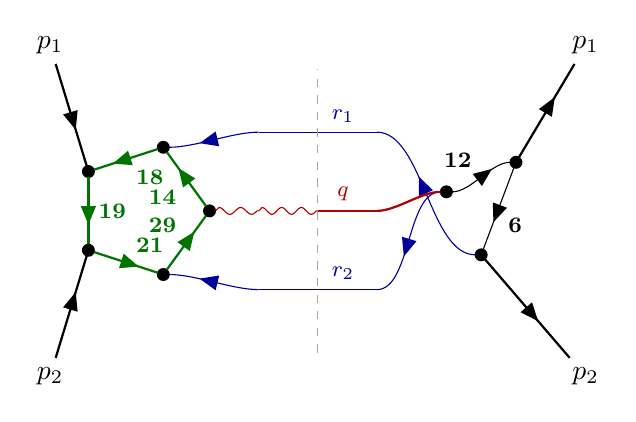
\begin{tikzpicture}
\begin{feynman}
\vertex (Lp1) at (-3.400,2.100) {$p_1$};
\vertex (Lp2) at (-3.400,-2.100) {$p_2$};
\vertex (Lcr1) at (-0.750,1.000);
\vertex (Lcr2) at (-0.750,-1.000);
\vertex (Lcq) at (-0.750,0.000);
\vertex (Mq) at (0,0.000);
\vertex[dot] (Lv0) at (-1.375,0.000) {};
\vertex[dot] (Lv1) at (-1.962,0.808) {};
\vertex[dot] (Lv2) at (-2.913,0.500) {};
\vertex[dot] (Lv3) at (-2.913,-0.500) {};
\vertex[dot] (Lv4) at (-1.962,-0.808) {};
\vertex (Rp1) at (3.400,2.100) {$p_1$};
\vertex (Rp2) at (3.400,-2.100) {$p_2$};
\vertex (Rcr1) at (0.750,1.000);
\vertex (Rcr2) at (0.750,-1.000);
\vertex (Rcq) at (0.750,0.000);
\vertex[dot] (R6) at (2.075,-0.558) {};
\vertex[dot] (R12) at (2.517,0.617) {};
\vertex[dot] (Rroot) at (1.633,0.242) {};
\diagram* {
(Lv0) -- [plain, thick, green!45!black, with arrow=0.55, edge label={\footnotesize\bfseries 14}] (Lv1),
(Lv1) -- [plain, thick, green!45!black, with arrow=0.55, edge label={\footnotesize\bfseries 18}] (Lv2),
(Lv2) -- [plain, thick, green!45!black, with arrow=0.55, edge label={\footnotesize\bfseries 19}] (Lv3),
(Lv3) -- [plain, thick, green!45!black, with arrow=0.55, edge label={\footnotesize\bfseries 21}] (Lv4),
(Lv4) -- [plain, thick, green!45!black, with arrow=0.55, edge label={\footnotesize\bfseries 29}] (Lv0),
(Lcq) -- [boson, red!70!black] (Lv0),
(Lcr1) -- [plain, blue!60!black, out=180, in=0, looseness=0.75, with arrow=0.55] (Lv1),
(Lp1) -- [plain, thick, with arrow=0.55] (Lv2),
(Lp2) -- [plain, thick, with arrow=0.55] (Lv3),
(Lcr2) -- [plain, blue!60!black, out=180, in=0, looseness=0.75, with arrow=0.55] (Lv4),
(R12) -- [plain, with arrow=0.55, edge label={\footnotesize\bfseries 6}] (R6),
(Rroot) -- [plain, out=0, in=180, looseness=0.75, with arrow=0.55, edge label={\footnotesize\bfseries 12}] (R12),
(R12) -- [plain, thick, with arrow=0.55] (Rp1),
(R6) -- [plain, thick, with arrow=0.55] (Rp2),
(R6) -- [plain, blue!60!black, out=180, in=0, looseness=0.75, with arrow=0.55] (Rcr1),
(Rroot) -- [plain, blue!60!black, out=180, in=0, looseness=0.75, with arrow=0.55] (Rcr2),
(Rroot) -- [plain, red!70!black, double, double distance=1.2pt, thick, out=180, in=0, looseness=0.75] (Rcq),
(Rcr1) -- [plain, blue!60!black] (Lcr1),
(Rcr2) -- [plain, blue!60!black] (Lcr2),
(Rcq) -- [plain, red!70!black, double, double distance=1.2pt, thick] (Mq) -- [boson, red!70!black] (Lcq),
};
\end{feynman}
\draw[dashed, gray!70] (0,-1.80) -- (0,1.80);
\node[font=\footnotesize, blue!60!black, above] at (0.32,1.00) {$r_1$};
\node[font=\footnotesize, blue!60!black, above] at (0.32,-1.00) {$r_2$};
\node[font=\footnotesize, red!70!black, above] at (0.32,0.00) {$q$};
\end{tikzpicture}}\\[2mm]\textbf{topo7} (RR family 24, pentagon q-r1-p1-p2-r2), sector with 7 of 8 lines\\[2pt]{\footnotesize\begin{tabular}{@{}r@{\ \ }l@{\ \ }l@{}}\textbf{14} & $(k_1)^2$ & loop\\
\textbf{18} & $(k_1+r_1)^2$ & loop\\
\textbf{19} & $(k_1+p_1+r_1)^2$ & loop\\
\textbf{21} & $(k_1+p_1+p_2+r_1)^2$ & loop\\
\textbf{29} & $(k_1+p_1+p_2+r_1+r_2)^2$ & loop\\
\textbf{6} & $(p_2+r_1)^2$ & conjugate\\
\textbf{12} & $(p_1+p_2+r_1)^2$ & conjugate\\\end{tabular}}\\[2pt]{\scriptsize pinched: 13 = $(p_1+p_2+r_2)^2$}\end{minipage}\hfill%
\begin{minipage}[t]{0.48\textwidth}\centering\resizebox{0.9\linewidth}{!}{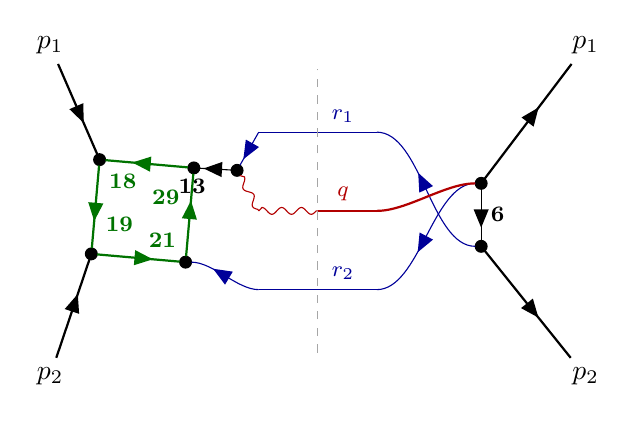
\begin{tikzpicture}
\begin{feynman}
\vertex (Lp1) at (-3.400,2.100) {$p_1$};
\vertex (Lp2) at (-3.400,-2.100) {$p_2$};
\vertex (Lcr1) at (-0.750,1.000);
\vertex (Lcr2) at (-0.750,-1.000);
\vertex (Lcq) at (-0.750,0.000);
\vertex (Mq) at (0,0.000);
\vertex[dot] (Lv0) at (-1.574,0.546) {};
\vertex[dot] (Lv1) at (-2.771,0.651) {};
\vertex[dot] (Lv2) at (-2.876,-0.546) {};
\vertex[dot] (Lv3) at (-1.679,-0.651) {};
\vertex[dot] (Lt13) at (-1.025,0.515) {};
\vertex (Rp1) at (3.400,2.100) {$p_1$};
\vertex (Rp2) at (3.400,-2.100) {$p_2$};
\vertex (Rcr1) at (0.750,1.000);
\vertex (Rcr2) at (0.750,-1.000);
\vertex (Rcq) at (0.750,0.000);
\vertex[dot] (R6) at (2.075,-0.450) {};
\vertex[dot] (Rroot) at (2.075,0.350) {};
\diagram* {
(Lv0) -- [plain, thick, green!45!black, with arrow=0.55, edge label={\footnotesize\bfseries 18}] (Lv1),
(Lv1) -- [plain, thick, green!45!black, with arrow=0.55, edge label={\footnotesize\bfseries 19}] (Lv2),
(Lv2) -- [plain, thick, green!45!black, with arrow=0.55, edge label={\footnotesize\bfseries 21}] (Lv3),
(Lv3) -- [plain, thick, green!45!black, with arrow=0.55, edge label={\footnotesize\bfseries 29}] (Lv0),
(Lt13) -- [plain, with arrow=0.55, edge label={\footnotesize\bfseries 13}] (Lv0),
(Lcr1) -- [plain, blue!60!black, with arrow=0.55] (Lt13),
(Lcq) -- [boson, red!70!black] (Lt13),
(Lp1) -- [plain, thick, with arrow=0.55] (Lv1),
(Lp2) -- [plain, thick, with arrow=0.55] (Lv2),
(Lcr2) -- [plain, blue!60!black, out=180, in=0, looseness=0.75, with arrow=0.55] (Lv3),
(Rroot) -- [plain, with arrow=0.55, edge label={\footnotesize\bfseries 6}] (R6),
(Rroot) -- [plain, thick, with arrow=0.55] (Rp1),
(R6) -- [plain, thick, with arrow=0.55] (Rp2),
(R6) -- [plain, blue!60!black, out=180, in=0, looseness=0.75, with arrow=0.55] (Rcr1),
(Rroot) -- [plain, blue!60!black, out=180, in=0, looseness=0.75, with arrow=0.55] (Rcr2),
(Rroot) -- [plain, red!70!black, double, double distance=1.2pt, thick, out=180, in=0, looseness=0.75] (Rcq),
(Rcr1) -- [plain, blue!60!black] (Lcr1),
(Rcr2) -- [plain, blue!60!black] (Lcr2),
(Rcq) -- [plain, red!70!black, double, double distance=1.2pt, thick] (Mq) -- [boson, red!70!black] (Lcq),
};
\end{feynman}
\draw[dashed, gray!70] (0,-1.80) -- (0,1.80);
\node[font=\footnotesize, blue!60!black, above] at (0.32,1.00) {$r_1$};
\node[font=\footnotesize, blue!60!black, above] at (0.32,-1.00) {$r_2$};
\node[font=\footnotesize, red!70!black, above] at (0.32,0.00) {$q$};
\end{tikzpicture}}\\[2mm]\textbf{topo7} (RR family 24, pentagon q-r1-p1-p2-r2), sector with 6 of 8 lines\\[2pt]{\footnotesize\begin{tabular}{@{}r@{\ \ }l@{\ \ }l@{}}\textbf{18} & $(k_1+r_1)^2$ & loop\\
\textbf{19} & $(k_1+p_1+r_1)^2$ & loop\\
\textbf{21} & $(k_1+p_1+p_2+r_1)^2$ & loop\\
\textbf{29} & $(k_1+p_1+p_2+r_1+r_2)^2$ & loop\\
\textbf{13} & $(p_1+p_2+r_2)^2$ & amplitude (tree on the loop)\\
\textbf{6} & $(p_2+r_1)^2$ & conjugate\\\end{tabular}}\\[2pt]{\scriptsize pinched: 12 = $(p_1+p_2+r_1)^2$, 14 = $(k_1)^2$}\end{minipage}

\bigskip

\begin{minipage}[t]{0.48\textwidth}\centering\resizebox{0.9\linewidth}{!}{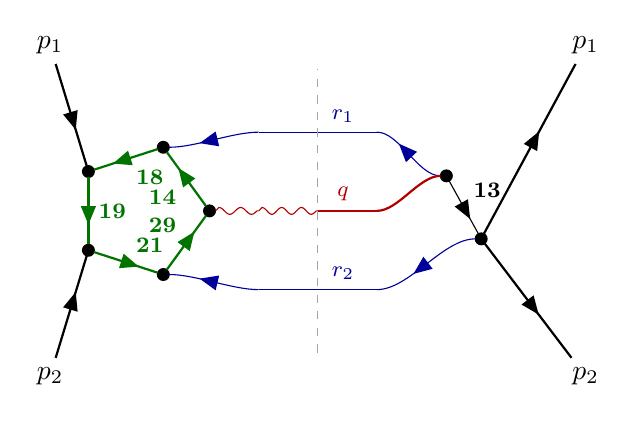
\begin{tikzpicture}
\begin{feynman}
\vertex (Lp1) at (-3.400,2.100) {$p_1$};
\vertex (Lp2) at (-3.400,-2.100) {$p_2$};
\vertex (Lcr1) at (-0.750,1.000);
\vertex (Lcr2) at (-0.750,-1.000);
\vertex (Lcq) at (-0.750,0.000);
\vertex (Mq) at (0,0.000);
\vertex[dot] (Lv0) at (-1.375,0.000) {};
\vertex[dot] (Lv1) at (-1.962,0.808) {};
\vertex[dot] (Lv2) at (-2.913,0.500) {};
\vertex[dot] (Lv3) at (-2.913,-0.500) {};
\vertex[dot] (Lv4) at (-1.962,-0.808) {};
\vertex (Rp1) at (3.400,2.100) {$p_1$};
\vertex (Rp2) at (3.400,-2.100) {$p_2$};
\vertex (Rcr1) at (0.750,1.000);
\vertex (Rcr2) at (0.750,-1.000);
\vertex (Rcq) at (0.750,0.000);
\vertex[dot] (R13) at (2.075,-0.355) {};
\vertex[dot] (Rroot) at (1.633,0.445) {};
\diagram* {
(Lv0) -- [plain, thick, green!45!black, with arrow=0.55, edge label={\footnotesize\bfseries 14}] (Lv1),
(Lv1) -- [plain, thick, green!45!black, with arrow=0.55, edge label={\footnotesize\bfseries 18}] (Lv2),
(Lv2) -- [plain, thick, green!45!black, with arrow=0.55, edge label={\footnotesize\bfseries 19}] (Lv3),
(Lv3) -- [plain, thick, green!45!black, with arrow=0.55, edge label={\footnotesize\bfseries 21}] (Lv4),
(Lv4) -- [plain, thick, green!45!black, with arrow=0.55, edge label={\footnotesize\bfseries 29}] (Lv0),
(Lcq) -- [boson, red!70!black] (Lv0),
(Lcr1) -- [plain, blue!60!black, out=180, in=0, looseness=0.75, with arrow=0.55] (Lv1),
(Lp1) -- [plain, thick, with arrow=0.55] (Lv2),
(Lp2) -- [plain, thick, with arrow=0.55] (Lv3),
(Lcr2) -- [plain, blue!60!black, out=180, in=0, looseness=0.75, with arrow=0.55] (Lv4),
(Rroot) -- [plain, with arrow=0.55, edge label={\footnotesize\bfseries 13}] (R13),
(R13) -- [plain, thick, with arrow=0.55] (Rp1),
(R13) -- [plain, thick, with arrow=0.55] (Rp2),
(Rroot) -- [plain, blue!60!black, out=180, in=0, looseness=0.75, with arrow=0.55] (Rcr1),
(R13) -- [plain, blue!60!black, out=180, in=0, looseness=0.75, with arrow=0.55] (Rcr2),
(Rroot) -- [plain, red!70!black, double, double distance=1.2pt, thick, out=180, in=0, looseness=0.75] (Rcq),
(Rcr1) -- [plain, blue!60!black] (Lcr1),
(Rcr2) -- [plain, blue!60!black] (Lcr2),
(Rcq) -- [plain, red!70!black, double, double distance=1.2pt, thick] (Mq) -- [boson, red!70!black] (Lcq),
};
\end{feynman}
\draw[dashed, gray!70] (0,-1.80) -- (0,1.80);
\node[font=\footnotesize, blue!60!black, above] at (0.32,1.00) {$r_1$};
\node[font=\footnotesize, blue!60!black, above] at (0.32,-1.00) {$r_2$};
\node[font=\footnotesize, red!70!black, above] at (0.32,0.00) {$q$};
\end{tikzpicture}}\\[2mm]\textbf{topo7} (RR family 24, pentagon q-r1-p1-p2-r2), sector with 6 of 8 lines\\[2pt]{\footnotesize\begin{tabular}{@{}r@{\ \ }l@{\ \ }l@{}}\textbf{14} & $(k_1)^2$ & loop\\
\textbf{18} & $(k_1+r_1)^2$ & loop\\
\textbf{19} & $(k_1+p_1+r_1)^2$ & loop\\
\textbf{21} & $(k_1+p_1+p_2+r_1)^2$ & loop\\
\textbf{29} & $(k_1+p_1+p_2+r_1+r_2)^2$ & loop\\
\textbf{13} & $(p_1+p_2+r_2)^2$ & conjugate\\\end{tabular}}\\[2pt]{\scriptsize pinched: 6 = $(p_2+r_1)^2$, 12 = $(p_1+p_2+r_1)^2$}\end{minipage}\hfill%
\begin{minipage}[t]{0.48\textwidth}\centering\resizebox{0.9\linewidth}{!}{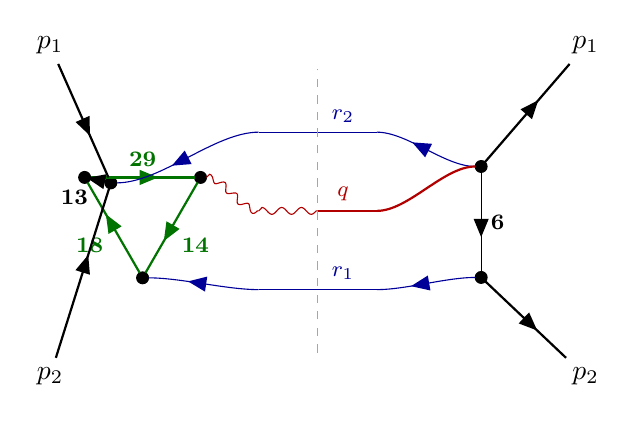
\begin{tikzpicture}
\begin{feynman}
\vertex (Lp1) at (-3.400,2.100) {$p_1$};
\vertex (Lp2) at (-3.400,-2.100) {$p_2$};
\vertex (Lcr1) at (-0.750,-1.000);
\vertex (Lcr2) at (-0.750,1.000);
\vertex (Lcq) at (-0.750,0.000);
\vertex (Mq) at (0,0.000);
\vertex[dot] (Lv0) at (-1.489,0.425) {};
\vertex[dot] (Lv1) at (-2.225,-0.850) {};
\vertex[dot] (Lv2) at (-2.961,0.425) {};
\vertex[dot] (Lt13) at (-2.628,0.356) {};
\vertex (Rp1) at (3.400,2.100) {$p_1$};
\vertex (Rp2) at (3.400,-2.100) {$p_2$};
\vertex (Rcr1) at (0.750,-1.000);
\vertex (Rcr2) at (0.750,1.000);
\vertex (Rcq) at (0.750,0.000);
\vertex[dot] (R6) at (2.075,-0.845) {};
\vertex[dot] (Rroot) at (2.075,0.564) {};
\diagram* {
(Lv0) -- [plain, thick, green!45!black, with arrow=0.55, edge label={\footnotesize\bfseries 14}] (Lv1),
(Lv1) -- [plain, thick, green!45!black, with arrow=0.55, edge label={\footnotesize\bfseries 18}] (Lv2),
(Lv2) -- [plain, thick, green!45!black, with arrow=0.55, edge label={\footnotesize\bfseries 29}] (Lv0),
(Lcq) -- [boson, red!70!black, out=180, in=0, looseness=0.75] (Lv0),
(Lcr1) -- [plain, blue!60!black, out=180, in=0, looseness=0.75, with arrow=0.55] (Lv1),
(Lt13) -- [plain, with arrow=0.55, edge label={\footnotesize\bfseries 13}] (Lv2),
(Lp2) -- [plain, thick, with arrow=0.55] (Lt13),
(Lcr2) -- [plain, blue!60!black, out=180, in=0, looseness=0.75, with arrow=0.55] (Lt13),
(Lp1) -- [plain, thick, with arrow=0.55] (Lt13),
(Rroot) -- [plain, with arrow=0.55, edge label={\footnotesize\bfseries 6}] (R6),
(Rroot) -- [plain, thick, with arrow=0.55] (Rp1),
(R6) -- [plain, thick, with arrow=0.55] (Rp2),
(R6) -- [plain, blue!60!black, out=180, in=0, looseness=0.75, with arrow=0.55] (Rcr1),
(Rroot) -- [plain, blue!60!black, out=180, in=0, looseness=0.75, with arrow=0.55] (Rcr2),
(Rroot) -- [plain, red!70!black, double, double distance=1.2pt, thick, out=180, in=0, looseness=0.75] (Rcq),
(Rcr1) -- [plain, blue!60!black] (Lcr1),
(Rcr2) -- [plain, blue!60!black] (Lcr2),
(Rcq) -- [plain, red!70!black, double, double distance=1.2pt, thick] (Mq) -- [boson, red!70!black] (Lcq),
};
\end{feynman}
\draw[dashed, gray!70] (0,-1.80) -- (0,1.80);
\node[font=\footnotesize, blue!60!black, above] at (0.32,-1.00) {$r_1$};
\node[font=\footnotesize, blue!60!black, above] at (0.32,1.00) {$r_2$};
\node[font=\footnotesize, red!70!black, above] at (0.32,0.00) {$q$};
\end{tikzpicture}}\\[2mm]\textbf{topo7} (RR family 24, pentagon q-r1-p1-p2-r2), sector with 5 of 8 lines\\[2pt]{\footnotesize\begin{tabular}{@{}r@{\ \ }l@{\ \ }l@{}}\textbf{14} & $(k_1)^2$ & loop\\
\textbf{18} & $(k_1+r_1)^2$ & loop\\
\textbf{29} & $(k_1+p_1+p_2+r_1+r_2)^2$ & loop\\
\textbf{13} & $(p_1+p_2+r_2)^2$ & amplitude (tree on the loop)\\
\textbf{6} & $(p_2+r_1)^2$ & conjugate\\\end{tabular}}\\[2pt]{\scriptsize pinched: 12 = $(p_1+p_2+r_1)^2$, 19 = $(k_1+p_1+r_1)^2$, 21 = $(k_1+p_1+p_2+r_1)^2$}\end{minipage}

\bigskip

\begin{minipage}[t]{0.48\textwidth}\centering\resizebox{0.9\linewidth}{!}{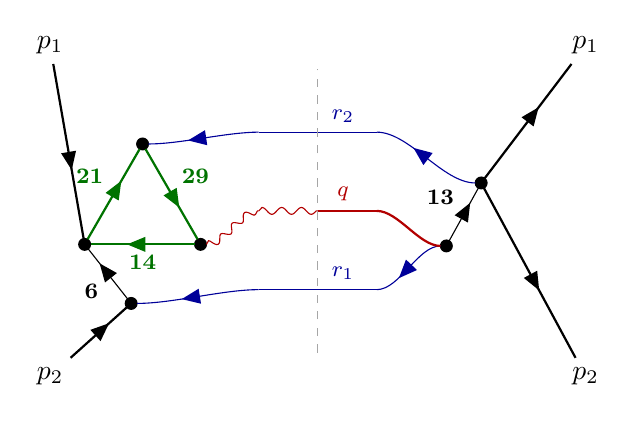
\begin{tikzpicture}
\begin{feynman}
\vertex (Lp1) at (-3.400,2.100) {$p_1$};
\vertex (Lp2) at (-3.400,-2.100) {$p_2$};
\vertex (Lcr1) at (-0.750,-1.000);
\vertex (Lcr2) at (-0.750,1.000);
\vertex (Lcq) at (-0.750,0.000);
\vertex (Mq) at (0,0.000);
\vertex[dot] (Lv0) at (-1.489,-0.425) {};
\vertex[dot] (Lv1) at (-2.961,-0.425) {};
\vertex[dot] (Lv2) at (-2.225,0.850) {};
\vertex[dot] (Lt6) at (-2.370,-1.175) {};
\vertex (Rp1) at (3.400,2.100) {$p_1$};
\vertex (Rp2) at (3.400,-2.100) {$p_2$};
\vertex (Rcr1) at (0.750,-1.000);
\vertex (Rcr2) at (0.750,1.000);
\vertex (Rcq) at (0.750,0.000);
\vertex[dot] (R13) at (2.075,0.355) {};
\vertex[dot] (Rroot) at (1.633,-0.445) {};
\diagram* {
(Lv0) -- [plain, thick, green!45!black, with arrow=0.55, edge label={\footnotesize\bfseries 14}] (Lv1),
(Lv1) -- [plain, thick, green!45!black, with arrow=0.55, edge label={\footnotesize\bfseries 21}] (Lv2),
(Lv2) -- [plain, thick, green!45!black, with arrow=0.55, edge label={\footnotesize\bfseries 29}] (Lv0),
(Lcq) -- [boson, red!70!black, out=180, in=0, looseness=0.75] (Lv0),
(Lt6) -- [plain, with arrow=0.55, edge label={\footnotesize\bfseries 6}] (Lv1),
(Lp2) -- [plain, thick, with arrow=0.55] (Lt6),
(Lcr1) -- [plain, blue!60!black, out=180, in=0, looseness=0.75, with arrow=0.55] (Lt6),
(Lp1) -- [plain, thick, with arrow=0.55] (Lv1),
(Lcr2) -- [plain, blue!60!black, out=180, in=0, looseness=0.75, with arrow=0.55] (Lv2),
(Rroot) -- [plain, with arrow=0.55, edge label={\footnotesize\bfseries 13}] (R13),
(R13) -- [plain, thick, with arrow=0.55] (Rp1),
(R13) -- [plain, thick, with arrow=0.55] (Rp2),
(Rroot) -- [plain, blue!60!black, out=180, in=0, looseness=0.75, with arrow=0.55] (Rcr1),
(R13) -- [plain, blue!60!black, out=180, in=0, looseness=0.75, with arrow=0.55] (Rcr2),
(Rroot) -- [plain, red!70!black, double, double distance=1.2pt, thick, out=180, in=0, looseness=0.75] (Rcq),
(Rcr1) -- [plain, blue!60!black] (Lcr1),
(Rcr2) -- [plain, blue!60!black] (Lcr2),
(Rcq) -- [plain, red!70!black, double, double distance=1.2pt, thick] (Mq) -- [boson, red!70!black] (Lcq),
};
\end{feynman}
\draw[dashed, gray!70] (0,-1.80) -- (0,1.80);
\node[font=\footnotesize, blue!60!black, above] at (0.32,-1.00) {$r_1$};
\node[font=\footnotesize, blue!60!black, above] at (0.32,1.00) {$r_2$};
\node[font=\footnotesize, red!70!black, above] at (0.32,0.00) {$q$};
\end{tikzpicture}}\\[2mm]\textbf{topo7} (RR family 24, pentagon q-r1-p1-p2-r2), sector with 5 of 8 lines\\[2pt]{\footnotesize\begin{tabular}{@{}r@{\ \ }l@{\ \ }l@{}}\textbf{14} & $(k_1)^2$ & loop\\
\textbf{21} & $(k_1+p_1+p_2+r_1)^2$ & loop\\
\textbf{29} & $(k_1+p_1+p_2+r_1+r_2)^2$ & loop\\
\textbf{6} & $(p_2+r_1)^2$ & amplitude (tree on the loop)\\
\textbf{13} & $(p_1+p_2+r_2)^2$ & conjugate\\\end{tabular}}\\[2pt]{\scriptsize pinched: 12 = $(p_1+p_2+r_1)^2$, 18 = $(k_1+r_1)^2$, 19 = $(k_1+p_1+r_1)^2$}\end{minipage}\hfill%
\begin{minipage}[t]{0.48\textwidth}\textbf{topo7} (RR family 24, pentagon q-r1-p1-p2-r2), sector with 4 of 8 lines\\[2pt]fewer than two loop lines: scaleless, zero{\footnotesize\begin{tabular}{@{}r@{\ \ }l@{\ \ }l@{}}\textbf{14} & $(k_1)^2$ & loop\\
\textbf{6} & $(p_2+r_1)^2$ & conjugate\\
\textbf{12} & $(p_1+p_2+r_1)^2$ & conjugate\\
\textbf{13} & $(p_1+p_2+r_2)^2$ & conjugate\\\end{tabular}}\\[2pt]{\scriptsize pinched: 18 = $(k_1+r_1)^2$, 19 = $(k_1+p_1+r_1)^2$, 21 = $(k_1+p_1+p_2+r_1)^2$, 29 = $(k_1+p_1+p_2+r_1+r_2)^2$}\end{minipage}

\bigskip

\begin{minipage}[t]{0.48\textwidth}\textbf{topo7} (RR family 24, pentagon q-r1-p1-p2-r2), sector with 4 of 8 lines\\[2pt]fewer than two loop lines: scaleless, zero{\footnotesize\begin{tabular}{@{}r@{\ \ }l@{\ \ }l@{}}\textbf{18} & $(k_1+r_1)^2$ & loop\\
\textbf{6} & $(p_2+r_1)^2$ & conjugate\\
\textbf{12} & $(p_1+p_2+r_1)^2$ & conjugate\\
\textbf{13} & $(p_1+p_2+r_2)^2$ & conjugate\\\end{tabular}}\\[2pt]{\scriptsize pinched: 14 = $(k_1)^2$, 19 = $(k_1+p_1+r_1)^2$, 21 = $(k_1+p_1+p_2+r_1)^2$, 29 = $(k_1+p_1+p_2+r_1+r_2)^2$}\end{minipage}\hfill%
\begin{minipage}[t]{0.48\textwidth}\textbf{topo7} (RR family 24, pentagon q-r1-p1-p2-r2), sector with 4 of 8 lines\\[2pt]fewer than two loop lines: scaleless, zero{\footnotesize\begin{tabular}{@{}r@{\ \ }l@{\ \ }l@{}}\textbf{21} & $(k_1+p_1+p_2+r_1)^2$ & loop\\
\textbf{6} & $(p_2+r_1)^2$ & conjugate\\
\textbf{12} & $(p_1+p_2+r_1)^2$ & conjugate\\
\textbf{13} & $(p_1+p_2+r_2)^2$ & conjugate\\\end{tabular}}\\[2pt]{\scriptsize pinched: 14 = $(k_1)^2$, 18 = $(k_1+r_1)^2$, 19 = $(k_1+p_1+r_1)^2$, 29 = $(k_1+p_1+p_2+r_1+r_2)^2$}\end{minipage}

\bigskip

\begin{minipage}[t]{0.48\textwidth}\textbf{topo7} (RR family 24, pentagon q-r1-p1-p2-r2), sector with 4 of 8 lines\\[2pt]fewer than two loop lines: scaleless, zero{\footnotesize\begin{tabular}{@{}r@{\ \ }l@{\ \ }l@{}}\textbf{29} & $(k_1+p_1+p_2+r_1+r_2)^2$ & loop\\
\textbf{6} & $(p_2+r_1)^2$ & conjugate\\
\textbf{12} & $(p_1+p_2+r_1)^2$ & conjugate\\
\textbf{13} & $(p_1+p_2+r_2)^2$ & conjugate\\\end{tabular}}\\[2pt]{\scriptsize pinched: 14 = $(k_1)^2$, 18 = $(k_1+r_1)^2$, 19 = $(k_1+p_1+r_1)^2$, 21 = $(k_1+p_1+p_2+r_1)^2$}\end{minipage}\hfill%
\begin{minipage}[t]{0.48\textwidth}\centering\resizebox{0.9\linewidth}{!}{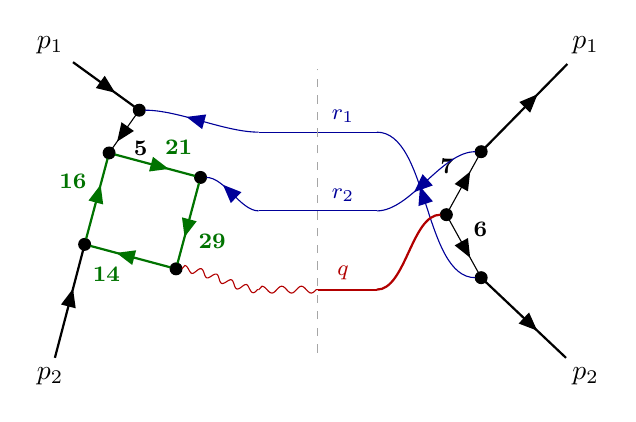
\begin{tikzpicture}
\begin{feynman}
\vertex (Lp1) at (-3.400,2.100) {$p_1$};
\vertex (Lp2) at (-3.400,-2.100) {$p_2$};
\vertex (Lcr1) at (-0.750,1.000);
\vertex (Lcr2) at (-0.750,0.000);
\vertex (Lcq) at (-0.750,-1.000);
\vertex (Mq) at (0,-1.000);
\vertex[dot] (Lv0) at (-1.800,-0.736) {};
\vertex[dot] (Lv1) at (-2.961,-0.425) {};
\vertex[dot] (Lv2) at (-2.650,0.736) {};
\vertex[dot] (Lv3) at (-1.489,0.425) {};
\vertex[dot] (Lt5) at (-2.267,1.279) {};
\vertex (Rp1) at (3.400,2.100) {$p_1$};
\vertex (Rp2) at (3.400,-2.100) {$p_2$};
\vertex (Rcr1) at (0.750,1.000);
\vertex (Rcr2) at (0.750,0.000);
\vertex (Rcq) at (0.750,-1.000);
\vertex[dot] (R6) at (2.075,-0.848) {};
\vertex[dot] (Rroot) at (1.633,-0.048) {};
\vertex[dot] (R7) at (2.075,0.752) {};
\diagram* {
(Lv0) -- [plain, thick, green!45!black, with arrow=0.55, edge label={\footnotesize\bfseries 14}] (Lv1),
(Lv1) -- [plain, thick, green!45!black, with arrow=0.55, edge label={\footnotesize\bfseries 16}] (Lv2),
(Lv2) -- [plain, thick, green!45!black, with arrow=0.55, edge label={\footnotesize\bfseries 21}] (Lv3),
(Lv3) -- [plain, thick, green!45!black, with arrow=0.55, edge label={\footnotesize\bfseries 29}] (Lv0),
(Lcq) -- [boson, red!70!black, out=180, in=0, looseness=0.75] (Lv0),
(Lp2) -- [plain, thick, with arrow=0.55] (Lv1),
(Lt5) -- [plain, with arrow=0.55, edge label={\footnotesize\bfseries 5}] (Lv2),
(Lcr1) -- [plain, blue!60!black, out=180, in=0, looseness=0.75, with arrow=0.55] (Lt5),
(Lp1) -- [plain, thick, with arrow=0.55] (Lt5),
(Lcr2) -- [plain, blue!60!black, out=180, in=0, looseness=0.75, with arrow=0.55] (Lv3),
(Rroot) -- [plain, with arrow=0.55, edge label={\footnotesize\bfseries 6}] (R6),
(Rroot) -- [plain, with arrow=0.55, edge label={\footnotesize\bfseries 7}] (R7),
(R7) -- [plain, thick, with arrow=0.55] (Rp1),
(R6) -- [plain, thick, with arrow=0.55] (Rp2),
(R6) -- [plain, blue!60!black, out=180, in=0, looseness=0.75, with arrow=0.55] (Rcr1),
(R7) -- [plain, blue!60!black, out=180, in=0, looseness=0.75, with arrow=0.55] (Rcr2),
(Rroot) -- [plain, red!70!black, double, double distance=1.2pt, thick, out=180, in=0, looseness=0.75] (Rcq),
(Rcr1) -- [plain, blue!60!black] (Lcr1),
(Rcr2) -- [plain, blue!60!black] (Lcr2),
(Rcq) -- [plain, red!70!black, double, double distance=1.2pt, thick] (Mq) -- [boson, red!70!black] (Lcq),
};
\end{feynman}
\draw[dashed, gray!70] (0,-1.80) -- (0,1.80);
\node[font=\footnotesize, blue!60!black, above] at (0.32,1.00) {$r_1$};
\node[font=\footnotesize, blue!60!black, above] at (0.32,0.00) {$r_2$};
\node[font=\footnotesize, red!70!black, above] at (0.32,-1.00) {$q$};
\end{tikzpicture}}\\[2mm]\textbf{topo8} (RR family 1, pentagon q-p2-r1-p1-r2), sector with 7 of 8 lines\\[2pt]{\footnotesize\begin{tabular}{@{}r@{\ \ }l@{\ \ }l@{}}\textbf{14} & $(k_1)^2$ & loop\\
\textbf{16} & $(k_1+p_2)^2$ & loop\\
\textbf{21} & $(k_1+p_1+p_2+r_1)^2$ & loop\\
\textbf{29} & $(k_1+p_1+p_2+r_1+r_2)^2$ & loop\\
\textbf{5} & $(p_1+r_1)^2$ & amplitude (tree on the loop)\\
\textbf{6} & $(p_2+r_1)^2$ & conjugate\\
\textbf{7} & $(p_1+r_2)^2$ & conjugate\\\end{tabular}}\\[2pt]{\scriptsize pinched: 20 = $(k_1+p_2+r_1)^2$}\end{minipage}

\bigskip

\begin{minipage}[t]{0.48\textwidth}\centering\resizebox{0.9\linewidth}{!}{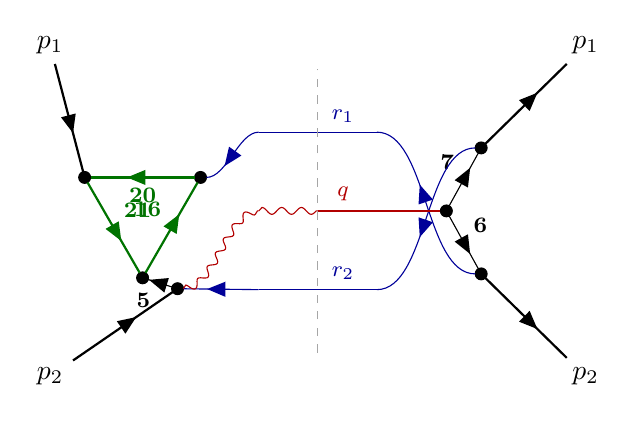
\begin{tikzpicture}
\begin{feynman}
\vertex (Lp1) at (-3.400,2.100) {$p_1$};
\vertex (Lp2) at (-3.400,-2.100) {$p_2$};
\vertex (Lcr1) at (-0.750,1.000);
\vertex (Lcr2) at (-0.750,-1.000);
\vertex (Lcq) at (-0.750,0.000);
\vertex (Mq) at (0,0.000);
\vertex[dot] (Lv0) at (-2.225,-0.850) {};
\vertex[dot] (Lv1) at (-1.489,0.425) {};
\vertex[dot] (Lv2) at (-2.961,0.425) {};
\vertex[dot] (Lt5) at (-1.781,-0.988) {};
\vertex (Rp1) at (3.400,2.100) {$p_1$};
\vertex (Rp2) at (3.400,-2.100) {$p_2$};
\vertex (Rcr1) at (0.750,1.000);
\vertex (Rcr2) at (0.750,-1.000);
\vertex (Rcq) at (0.750,0.000);
\vertex[dot] (R6) at (2.075,-0.800) {};
\vertex[dot] (Rroot) at (1.633,-0.000) {};
\vertex[dot] (R7) at (2.075,0.800) {};
\diagram* {
(Lv0) -- [plain, thick, green!45!black, with arrow=0.55, edge label={\footnotesize\bfseries 16}] (Lv1),
(Lv1) -- [plain, thick, green!45!black, with arrow=0.55, edge label={\footnotesize\bfseries 20}] (Lv2),
(Lv2) -- [plain, thick, green!45!black, with arrow=0.55, edge label={\footnotesize\bfseries 21}] (Lv0),
(Lt5) -- [plain, with arrow=0.55, edge label={\footnotesize\bfseries 5}] (Lv0),
(Lp2) -- [plain, thick, with arrow=0.55] (Lt5),
(Lcr2) -- [plain, blue!60!black, with arrow=0.55] (Lt5),
(Lcq) -- [boson, red!70!black, out=180, in=0, looseness=0.75] (Lt5),
(Lcr1) -- [plain, blue!60!black, out=180, in=0, looseness=0.75, with arrow=0.55] (Lv1),
(Lp1) -- [plain, thick, with arrow=0.55] (Lv2),
(Rroot) -- [plain, with arrow=0.55, edge label={\footnotesize\bfseries 6}] (R6),
(Rroot) -- [plain, with arrow=0.55, edge label={\footnotesize\bfseries 7}] (R7),
(R7) -- [plain, thick, with arrow=0.55] (Rp1),
(R6) -- [plain, thick, with arrow=0.55] (Rp2),
(R6) -- [plain, blue!60!black, out=180, in=0, looseness=0.75, with arrow=0.55] (Rcr1),
(R7) -- [plain, blue!60!black, out=180, in=0, looseness=0.75, with arrow=0.55] (Rcr2),
(Rroot) -- [plain, red!70!black, double, double distance=1.2pt, thick] (Rcq),
(Rcr1) -- [plain, blue!60!black] (Lcr1),
(Rcr2) -- [plain, blue!60!black] (Lcr2),
(Rcq) -- [plain, red!70!black, double, double distance=1.2pt, thick] (Mq) -- [boson, red!70!black] (Lcq),
};
\end{feynman}
\draw[dashed, gray!70] (0,-1.80) -- (0,1.80);
\node[font=\footnotesize, blue!60!black, above] at (0.32,1.00) {$r_1$};
\node[font=\footnotesize, blue!60!black, above] at (0.32,-1.00) {$r_2$};
\node[font=\footnotesize, red!70!black, above] at (0.32,0.00) {$q$};
\end{tikzpicture}}\\[2mm]\textbf{topo8} (RR family 1, pentagon q-p2-r1-p1-r2), sector with 6 of 8 lines\\[2pt]{\footnotesize\begin{tabular}{@{}r@{\ \ }l@{\ \ }l@{}}\textbf{16} & $(k_1+p_2)^2$ & loop\\
\textbf{20} & $(k_1+p_2+r_1)^2$ & loop\\
\textbf{21} & $(k_1+p_1+p_2+r_1)^2$ & loop\\
\textbf{5} & $(p_1+r_1)^2$ & amplitude (tree on the loop)\\
\textbf{6} & $(p_2+r_1)^2$ & conjugate\\
\textbf{7} & $(p_1+r_2)^2$ & conjugate\\\end{tabular}}\\[2pt]{\scriptsize pinched: 14 = $(k_1)^2$, 29 = $(k_1+p_1+p_2+r_1+r_2)^2$}\end{minipage}\hfill%
\begin{minipage}[t]{0.48\textwidth}\centering\resizebox{0.9\linewidth}{!}{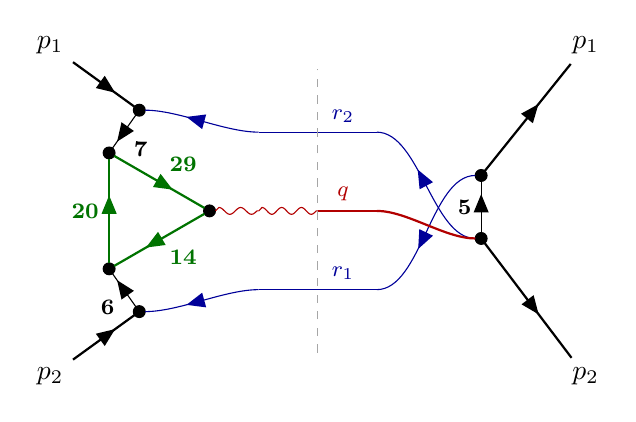
\begin{tikzpicture}
\begin{feynman}
\vertex (Lp1) at (-3.400,2.100) {$p_1$};
\vertex (Lp2) at (-3.400,-2.100) {$p_2$};
\vertex (Lcr1) at (-0.750,-1.000);
\vertex (Lcr2) at (-0.750,1.000);
\vertex (Lcq) at (-0.750,0.000);
\vertex (Mq) at (0,0.000);
\vertex[dot] (Lv0) at (-1.375,0.000) {};
\vertex[dot] (Lv1) at (-2.650,-0.736) {};
\vertex[dot] (Lv2) at (-2.650,0.736) {};
\vertex[dot] (Lt6) at (-2.267,-1.279) {};
\vertex[dot] (Lt7) at (-2.267,1.279) {};
\vertex (Rp1) at (3.400,2.100) {$p_1$};
\vertex (Rp2) at (3.400,-2.100) {$p_2$};
\vertex (Rcr1) at (0.750,-1.000);
\vertex (Rcr2) at (0.750,1.000);
\vertex (Rcq) at (0.750,0.000);
\vertex[dot] (R5) at (2.075,0.450) {};
\vertex[dot] (Rroot) at (2.075,-0.350) {};
\diagram* {
(Lv0) -- [plain, thick, green!45!black, with arrow=0.55, edge label={\footnotesize\bfseries 14}] (Lv1),
(Lv1) -- [plain, thick, green!45!black, with arrow=0.55, edge label={\footnotesize\bfseries 20}] (Lv2),
(Lv2) -- [plain, thick, green!45!black, with arrow=0.55, edge label={\footnotesize\bfseries 29}] (Lv0),
(Lcq) -- [boson, red!70!black] (Lv0),
(Lt6) -- [plain, with arrow=0.55, edge label={\footnotesize\bfseries 6}] (Lv1),
(Lp2) -- [plain, thick, with arrow=0.55] (Lt6),
(Lcr1) -- [plain, blue!60!black, out=180, in=0, looseness=0.75, with arrow=0.55] (Lt6),
(Lt7) -- [plain, with arrow=0.55, edge label={\footnotesize\bfseries 7}] (Lv2),
(Lcr2) -- [plain, blue!60!black, out=180, in=0, looseness=0.75, with arrow=0.55] (Lt7),
(Lp1) -- [plain, thick, with arrow=0.55] (Lt7),
(Rroot) -- [plain, with arrow=0.55, edge label={\footnotesize\bfseries 5}] (R5),
(R5) -- [plain, thick, with arrow=0.55] (Rp1),
(Rroot) -- [plain, thick, with arrow=0.55] (Rp2),
(R5) -- [plain, blue!60!black, out=180, in=0, looseness=0.75, with arrow=0.55] (Rcr1),
(Rroot) -- [plain, blue!60!black, out=180, in=0, looseness=0.75, with arrow=0.55] (Rcr2),
(Rroot) -- [plain, red!70!black, double, double distance=1.2pt, thick, out=180, in=0, looseness=0.75] (Rcq),
(Rcr1) -- [plain, blue!60!black] (Lcr1),
(Rcr2) -- [plain, blue!60!black] (Lcr2),
(Rcq) -- [plain, red!70!black, double, double distance=1.2pt, thick] (Mq) -- [boson, red!70!black] (Lcq),
};
\end{feynman}
\draw[dashed, gray!70] (0,-1.80) -- (0,1.80);
\node[font=\footnotesize, blue!60!black, above] at (0.32,-1.00) {$r_1$};
\node[font=\footnotesize, blue!60!black, above] at (0.32,1.00) {$r_2$};
\node[font=\footnotesize, red!70!black, above] at (0.32,0.00) {$q$};
\end{tikzpicture}}\\[2mm]\textbf{topo8} (RR family 1, pentagon q-p2-r1-p1-r2), sector with 6 of 8 lines\\[2pt]{\footnotesize\begin{tabular}{@{}r@{\ \ }l@{\ \ }l@{}}\textbf{14} & $(k_1)^2$ & loop\\
\textbf{20} & $(k_1+p_2+r_1)^2$ & loop\\
\textbf{29} & $(k_1+p_1+p_2+r_1+r_2)^2$ & loop\\
\textbf{6} & $(p_2+r_1)^2$ & amplitude (tree on the loop)\\
\textbf{7} & $(p_1+r_2)^2$ & amplitude (tree on the loop)\\
\textbf{5} & $(p_1+r_1)^2$ & conjugate\\\end{tabular}}\\[2pt]{\scriptsize pinched: 16 = $(k_1+p_2)^2$, 21 = $(k_1+p_1+p_2+r_1)^2$}\end{minipage}

\bigskip

\begin{minipage}[t]{0.48\textwidth}\centering\resizebox{0.9\linewidth}{!}{\begin{tikzpicture}
\begin{feynman}
\vertex (Lp1) at (-3.400,2.100) {$p_1$};
\vertex (Lp2) at (-3.400,-2.100) {$p_2$};
\vertex (Lcr1) at (-0.750,1.000);
\vertex (Lcr2) at (-0.750,-1.000);
\vertex (Lcq) at (-0.750,0.000);
\vertex (Mq) at (0,0.000);
\vertex[dot] (Lv0) at (-1.679,-0.651) {};
\vertex[dot] (Lv1) at (-2.876,-0.546) {};
\vertex[dot] (Lv2) at (-2.771,0.651) {};
\vertex[dot] (Lv3) at (-1.574,0.546) {};
\vertex[dot] (Lt7) at (-1.908,0.549) {};
\vertex (Rp1) at (3.400,2.100) {$p_1$};
\vertex (Rp2) at (3.400,-2.100) {$p_2$};
\vertex (Rcr1) at (0.750,1.000);
\vertex (Rcr2) at (0.750,-1.000);
\vertex (Rcq) at (0.750,0.000);
\vertex[dot] (R5) at (2.075,0.845) {};
\vertex[dot] (Rroot) at (2.075,-0.564) {};
\diagram* {
(Lv0) -- [plain, thick, green!45!black, with arrow=0.55, edge label={\footnotesize\bfseries 14}] (Lv1),
(Lv1) -- [plain, thick, green!45!black, with arrow=0.55, edge label={\footnotesize\bfseries 16}] (Lv2),
(Lv2) -- [plain, thick, green!45!black, with arrow=0.55, edge label={\footnotesize\bfseries 20}] (Lv3),
(Lv3) -- [plain, thick, green!45!black, with arrow=0.55, edge label={\footnotesize\bfseries 29}] (Lv0),
(Lcq) -- [boson, red!70!black, out=180, in=0, looseness=0.75] (Lv0),
(Lp2) -- [plain, thick, with arrow=0.55] (Lv1),
(Lcr1) -- [plain, blue!60!black, out=180, in=0, looseness=0.75, with arrow=0.55] (Lv2),
(Lt7) -- [plain, with arrow=0.55, edge label={\footnotesize\bfseries 7}] (Lv3),
(Lcr2) -- [plain, blue!60!black, out=180, in=0, looseness=0.75, with arrow=0.55] (Lt7),
(Lp1) -- [plain, thick, with arrow=0.55] (Lt7),
(Rroot) -- [plain, with arrow=0.55, edge label={\footnotesize\bfseries 5}] (R5),
(R5) -- [plain, thick, with arrow=0.55] (Rp1),
(Rroot) -- [plain, thick, with arrow=0.55] (Rp2),
(R5) -- [plain, blue!60!black, out=180, in=0, looseness=0.75, with arrow=0.55] (Rcr1),
(Rroot) -- [plain, blue!60!black, out=180, in=0, looseness=0.75, with arrow=0.55] (Rcr2),
(Rroot) -- [plain, red!70!black, double, double distance=1.2pt, thick, out=180, in=0, looseness=0.75] (Rcq),
(Rcr1) -- [plain, blue!60!black] (Lcr1),
(Rcr2) -- [plain, blue!60!black] (Lcr2),
(Rcq) -- [plain, red!70!black, double, double distance=1.2pt, thick] (Mq) -- [boson, red!70!black] (Lcq),
};
\end{feynman}
\draw[dashed, gray!70] (0,-1.80) -- (0,1.80);
\node[font=\footnotesize, blue!60!black, above] at (0.32,1.00) {$r_1$};
\node[font=\footnotesize, blue!60!black, above] at (0.32,-1.00) {$r_2$};
\node[font=\footnotesize, red!70!black, above] at (0.32,0.00) {$q$};
\end{tikzpicture}}\\[2mm]\textbf{topo8} (RR family 1, pentagon q-p2-r1-p1-r2), sector with 6 of 8 lines\\[2pt]{\footnotesize\begin{tabular}{@{}r@{\ \ }l@{\ \ }l@{}}\textbf{14} & $(k_1)^2$ & loop\\
\textbf{16} & $(k_1+p_2)^2$ & loop\\
\textbf{20} & $(k_1+p_2+r_1)^2$ & loop\\
\textbf{29} & $(k_1+p_1+p_2+r_1+r_2)^2$ & loop\\
\textbf{7} & $(p_1+r_2)^2$ & amplitude (tree on the loop)\\
\textbf{5} & $(p_1+r_1)^2$ & conjugate\\\end{tabular}}\\[2pt]{\scriptsize pinched: 6 = $(p_2+r_1)^2$, 21 = $(k_1+p_1+p_2+r_1)^2$}\end{minipage}\hfill%
\begin{minipage}[t]{0.48\textwidth}\centering\resizebox{0.9\linewidth}{!}{\begin{tikzpicture}
\begin{feynman}
\vertex (Lp1) at (-3.400,2.100) {$p_1$};
\vertex (Lp2) at (-3.400,-2.100) {$p_2$};
\vertex (Lcr1) at (-0.750,-1.000);
\vertex (Lcr2) at (-0.750,1.000);
\vertex (Lcq) at (-0.750,0.000);
\vertex (Mq) at (0,0.000);
\vertex[dot] (Lv0) at (-1.489,-0.425) {};
\vertex[dot] (Lv1) at (-2.650,-0.736) {};
\vertex[dot] (Lv2) at (-2.961,0.425) {};
\vertex[dot] (Lv3) at (-1.800,0.736) {};
\vertex[dot] (Lt6) at (-2.267,-1.279) {};
\vertex (Rp1) at (3.400,2.100) {$p_1$};
\vertex (Rp2) at (3.400,-2.100) {$p_2$};
\vertex (Rcr1) at (0.750,-1.000);
\vertex (Rcr2) at (0.750,1.000);
\vertex (Rcq) at (0.750,0.000);
\vertex[dot] (R5) at (2.075,0.450) {};
\vertex[dot] (Rroot) at (2.075,-0.350) {};
\diagram* {
(Lv0) -- [plain, thick, green!45!black, with arrow=0.55, edge label={\footnotesize\bfseries 14}] (Lv1),
(Lv1) -- [plain, thick, green!45!black, with arrow=0.55, edge label={\footnotesize\bfseries 20}] (Lv2),
(Lv2) -- [plain, thick, green!45!black, with arrow=0.55, edge label={\footnotesize\bfseries 21}] (Lv3),
(Lv3) -- [plain, thick, green!45!black, with arrow=0.55, edge label={\footnotesize\bfseries 29}] (Lv0),
(Lcq) -- [boson, red!70!black, out=180, in=0, looseness=0.75] (Lv0),
(Lt6) -- [plain, with arrow=0.55, edge label={\footnotesize\bfseries 6}] (Lv1),
(Lp2) -- [plain, thick, with arrow=0.55] (Lt6),
(Lcr1) -- [plain, blue!60!black, out=180, in=0, looseness=0.75, with arrow=0.55] (Lt6),
(Lp1) -- [plain, thick, with arrow=0.55] (Lv2),
(Lcr2) -- [plain, blue!60!black, out=180, in=0, looseness=0.75, with arrow=0.55] (Lv3),
(Rroot) -- [plain, with arrow=0.55, edge label={\footnotesize\bfseries 5}] (R5),
(R5) -- [plain, thick, with arrow=0.55] (Rp1),
(Rroot) -- [plain, thick, with arrow=0.55] (Rp2),
(R5) -- [plain, blue!60!black, out=180, in=0, looseness=0.75, with arrow=0.55] (Rcr1),
(Rroot) -- [plain, blue!60!black, out=180, in=0, looseness=0.75, with arrow=0.55] (Rcr2),
(Rroot) -- [plain, red!70!black, double, double distance=1.2pt, thick, out=180, in=0, looseness=0.75] (Rcq),
(Rcr1) -- [plain, blue!60!black] (Lcr1),
(Rcr2) -- [plain, blue!60!black] (Lcr2),
(Rcq) -- [plain, red!70!black, double, double distance=1.2pt, thick] (Mq) -- [boson, red!70!black] (Lcq),
};
\end{feynman}
\draw[dashed, gray!70] (0,-1.80) -- (0,1.80);
\node[font=\footnotesize, blue!60!black, above] at (0.32,-1.00) {$r_1$};
\node[font=\footnotesize, blue!60!black, above] at (0.32,1.00) {$r_2$};
\node[font=\footnotesize, red!70!black, above] at (0.32,0.00) {$q$};
\end{tikzpicture}}\\[2mm]\textbf{topo8} (RR family 1, pentagon q-p2-r1-p1-r2), sector with 6 of 8 lines\\[2pt]{\footnotesize\begin{tabular}{@{}r@{\ \ }l@{\ \ }l@{}}\textbf{14} & $(k_1)^2$ & loop\\
\textbf{20} & $(k_1+p_2+r_1)^2$ & loop\\
\textbf{21} & $(k_1+p_1+p_2+r_1)^2$ & loop\\
\textbf{29} & $(k_1+p_1+p_2+r_1+r_2)^2$ & loop\\
\textbf{6} & $(p_2+r_1)^2$ & amplitude (tree on the loop)\\
\textbf{5} & $(p_1+r_1)^2$ & conjugate\\\end{tabular}}\\[2pt]{\scriptsize pinched: 7 = $(p_1+r_2)^2$, 16 = $(k_1+p_2)^2$}\end{minipage}

\bigskip

\begin{minipage}[t]{0.48\textwidth}\centering\resizebox{0.9\linewidth}{!}{\begin{tikzpicture}
\begin{feynman}
\vertex (Lp1) at (-3.400,2.100) {$p_1$};
\vertex (Lp2) at (-3.400,-2.100) {$p_2$};
\vertex (Lcr1) at (-0.750,-1.000);
\vertex (Lcr2) at (-0.750,1.000);
\vertex (Lcq) at (-0.750,0.000);
\vertex (Mq) at (0,0.000);
\vertex[dot] (Lv0) at (-1.426,0.291) {};
\vertex[dot] (Lv1) at (-2.373,-0.837) {};
\vertex[dot] (Lv2) at (-2.876,0.546) {};
\vertex (Rp1) at (3.400,2.100) {$p_1$};
\vertex (Rp2) at (3.400,-2.100) {$p_2$};
\vertex (Rcr1) at (0.750,-1.000);
\vertex (Rcr2) at (0.750,1.000);
\vertex (Rcq) at (0.750,0.000);
\vertex[dot] (R6) at (2.075,-1.033) {};
\vertex[dot] (Rroot) at (1.633,0.000) {};
\vertex[dot] (R7) at (2.075,1.033) {};
\diagram* {
(Lv0) -- [plain, thick, green!45!black, with arrow=0.55, edge label={\footnotesize\bfseries 14}] (Lv1),
(Lv1) -- [plain, thick, green!45!black, with arrow=0.55, edge label={\footnotesize\bfseries 20}] (Lv2),
(Lv2) -- [plain, thick, green!45!black, with arrow=0.55, edge label={\footnotesize\bfseries 21}] (Lv0),
(Lcr2) -- [plain, blue!60!black, with arrow=0.55] (Lv0),
(Lcq) -- [boson, red!70!black] (Lv0),
(Lp2) -- [plain, thick, with arrow=0.55] (Lv1),
(Lcr1) -- [plain, blue!60!black, out=180, in=0, looseness=0.75, with arrow=0.55] (Lv1),
(Lp1) -- [plain, thick, with arrow=0.55] (Lv2),
(Rroot) -- [plain, with arrow=0.55, edge label={\footnotesize\bfseries 6}] (R6),
(Rroot) -- [plain, with arrow=0.55, edge label={\footnotesize\bfseries 7}] (R7),
(R7) -- [plain, thick, with arrow=0.55] (Rp1),
(R6) -- [plain, thick, with arrow=0.55] (Rp2),
(R6) -- [plain, blue!60!black, with arrow=0.55] (Rcr1),
(R7) -- [plain, blue!60!black, with arrow=0.55] (Rcr2),
(Rroot) -- [plain, red!70!black, double, double distance=1.2pt, thick] (Rcq),
(Rcr1) -- [plain, blue!60!black] (Lcr1),
(Rcr2) -- [plain, blue!60!black] (Lcr2),
(Rcq) -- [plain, red!70!black, double, double distance=1.2pt, thick] (Mq) -- [boson, red!70!black] (Lcq),
};
\end{feynman}
\draw[dashed, gray!70] (0,-1.80) -- (0,1.80);
\node[font=\footnotesize, blue!60!black, above] at (0.32,-1.00) {$r_1$};
\node[font=\footnotesize, blue!60!black, above] at (0.32,1.00) {$r_2$};
\node[font=\footnotesize, red!70!black, above] at (0.32,0.00) {$q$};
\end{tikzpicture}}\\[2mm]\textbf{topo8} (RR family 1, pentagon q-p2-r1-p1-r2), sector with 5 of 8 lines\\[2pt]{\footnotesize\begin{tabular}{@{}r@{\ \ }l@{\ \ }l@{}}\textbf{14} & $(k_1)^2$ & loop\\
\textbf{20} & $(k_1+p_2+r_1)^2$ & loop\\
\textbf{21} & $(k_1+p_1+p_2+r_1)^2$ & loop\\
\textbf{6} & $(p_2+r_1)^2$ & conjugate\\
\textbf{7} & $(p_1+r_2)^2$ & conjugate\\\end{tabular}}\\[2pt]{\scriptsize pinched: 5 = $(p_1+r_1)^2$, 16 = $(k_1+p_2)^2$, 29 = $(k_1+p_1+p_2+r_1+r_2)^2$}\end{minipage}\hfill%
\begin{minipage}[t]{0.48\textwidth}\centering\resizebox{0.9\linewidth}{!}{\begin{tikzpicture}
\begin{feynman}
\vertex (Lp1) at (-3.400,2.100) {$p_1$};
\vertex (Lp2) at (-3.400,-2.100) {$p_2$};
\vertex (Lcr1) at (-0.750,-1.000);
\vertex (Lcr2) at (-0.750,1.000);
\vertex (Lcq) at (-0.750,0.000);
\vertex (Mq) at (0,0.000);
\vertex[dot] (Lv0) at (-1.574,0.546) {};
\vertex[dot] (Lv1) at (-1.679,-0.651) {};
\vertex[dot] (Lv2) at (-2.876,-0.546) {};
\vertex[dot] (Lv3) at (-2.771,0.651) {};
\vertex (Rp1) at (3.400,2.100) {$p_1$};
\vertex (Rp2) at (3.400,-2.100) {$p_2$};
\vertex (Rcr1) at (0.750,-1.000);
\vertex (Rcr2) at (0.750,1.000);
\vertex (Rcq) at (0.750,0.000);
\vertex[dot] (R7) at (2.075,0.845) {};
\vertex[dot] (Rroot) at (2.075,-0.564) {};
\diagram* {
(Lv0) -- [plain, thick, green!45!black, with arrow=0.55, edge label={\footnotesize\bfseries 14}] (Lv1),
(Lv1) -- [plain, thick, green!45!black, with arrow=0.55, edge label={\footnotesize\bfseries 16}] (Lv2),
(Lv2) -- [plain, thick, green!45!black, with arrow=0.55, edge label={\footnotesize\bfseries 20}] (Lv3),
(Lv3) -- [plain, thick, green!45!black, with arrow=0.55, edge label={\footnotesize\bfseries 21}] (Lv0),
(Lcr2) -- [plain, blue!60!black, out=180, in=0, looseness=0.75, with arrow=0.55] (Lv0),
(Lcq) -- [boson, red!70!black, out=180, in=0, looseness=0.75] (Lv0),
(Lp2) -- [plain, thick, with arrow=0.55] (Lv1),
(Lcr1) -- [plain, blue!60!black, out=180, in=0, looseness=0.75, with arrow=0.55] (Lv2),
(Lp1) -- [plain, thick, with arrow=0.55] (Lv3),
(Rroot) -- [plain, with arrow=0.55, edge label={\footnotesize\bfseries 7}] (R7),
(R7) -- [plain, thick, with arrow=0.55] (Rp1),
(Rroot) -- [plain, thick, with arrow=0.55] (Rp2),
(Rroot) -- [plain, blue!60!black, out=180, in=0, looseness=0.75, with arrow=0.55] (Rcr1),
(R7) -- [plain, blue!60!black, out=180, in=0, looseness=0.75, with arrow=0.55] (Rcr2),
(Rroot) -- [plain, red!70!black, double, double distance=1.2pt, thick, out=180, in=0, looseness=0.75] (Rcq),
(Rcr1) -- [plain, blue!60!black] (Lcr1),
(Rcr2) -- [plain, blue!60!black] (Lcr2),
(Rcq) -- [plain, red!70!black, double, double distance=1.2pt, thick] (Mq) -- [boson, red!70!black] (Lcq),
};
\end{feynman}
\draw[dashed, gray!70] (0,-1.80) -- (0,1.80);
\node[font=\footnotesize, blue!60!black, above] at (0.32,-1.00) {$r_1$};
\node[font=\footnotesize, blue!60!black, above] at (0.32,1.00) {$r_2$};
\node[font=\footnotesize, red!70!black, above] at (0.32,0.00) {$q$};
\end{tikzpicture}}\\[2mm]\textbf{topo8} (RR family 1, pentagon q-p2-r1-p1-r2), sector with 5 of 8 lines\\[2pt]{\footnotesize\begin{tabular}{@{}r@{\ \ }l@{\ \ }l@{}}\textbf{14} & $(k_1)^2$ & loop\\
\textbf{16} & $(k_1+p_2)^2$ & loop\\
\textbf{20} & $(k_1+p_2+r_1)^2$ & loop\\
\textbf{21} & $(k_1+p_1+p_2+r_1)^2$ & loop\\
\textbf{7} & $(p_1+r_2)^2$ & conjugate\\\end{tabular}}\\[2pt]{\scriptsize pinched: 5 = $(p_1+r_1)^2$, 6 = $(p_2+r_1)^2$, 29 = $(k_1+p_1+p_2+r_1+r_2)^2$}\end{minipage}

\bigskip

\begin{minipage}[t]{0.48\textwidth}\centering\resizebox{0.9\linewidth}{!}{\begin{tikzpicture}
\begin{feynman}
\vertex (Lp1) at (-3.400,2.100) {$p_1$};
\vertex (Lp2) at (-3.400,-2.100) {$p_2$};
\vertex (Lcr1) at (-0.750,0.000);
\vertex (Lcr2) at (-0.750,1.000);
\vertex (Lcq) at (-0.750,-1.000);
\vertex (Mq) at (0,-1.000);
\vertex[dot] (Lv0) at (-2.650,-0.736) {};
\vertex[dot] (Lv1) at (-1.375,-0.000) {};
\vertex[dot] (Lv2) at (-2.650,0.736) {};
\vertex (Rp1) at (3.400,2.100) {$p_1$};
\vertex (Rp2) at (3.400,-2.100) {$p_2$};
\vertex (Rcr1) at (0.750,0.000);
\vertex (Rcr2) at (0.750,1.000);
\vertex (Rcq) at (0.750,-1.000);
\vertex[dot] (R6) at (2.075,-0.940) {};
\vertex[dot] (Rroot) at (1.633,-0.140) {};
\vertex[dot] (R7) at (2.075,0.938) {};
\diagram* {
(Lv0) -- [plain, thick, green!45!black, with arrow=0.55, edge label={\footnotesize\bfseries 16}] (Lv1),
(Lv1) -- [plain, thick, green!45!black, with arrow=0.55, edge label={\footnotesize\bfseries 20}] (Lv2),
(Lv2) -- [plain, thick, green!45!black, with arrow=0.55, edge label={\footnotesize\bfseries 29}] (Lv0),
(Lp2) -- [plain, thick, with arrow=0.55] (Lv0),
(Lcq) -- [boson, red!70!black, out=180, in=0, looseness=0.75] (Lv0),
(Lcr1) -- [plain, blue!60!black, with arrow=0.55] (Lv1),
(Lcr2) -- [plain, blue!60!black, out=180, in=0, looseness=0.75, with arrow=0.55] (Lv2),
(Lp1) -- [plain, thick, with arrow=0.55] (Lv2),
(Rroot) -- [plain, with arrow=0.55, edge label={\footnotesize\bfseries 6}] (R6),
(Rroot) -- [plain, with arrow=0.55, edge label={\footnotesize\bfseries 7}] (R7),
(R7) -- [plain, thick, with arrow=0.55] (Rp1),
(R6) -- [plain, thick, with arrow=0.55] (Rp2),
(R6) -- [plain, blue!60!black, out=180, in=0, looseness=0.75, with arrow=0.55] (Rcr1),
(R7) -- [plain, blue!60!black, out=180, in=0, looseness=0.75, with arrow=0.55] (Rcr2),
(Rroot) -- [plain, red!70!black, double, double distance=1.2pt, thick, out=180, in=0, looseness=0.75] (Rcq),
(Rcr1) -- [plain, blue!60!black] (Lcr1),
(Rcr2) -- [plain, blue!60!black] (Lcr2),
(Rcq) -- [plain, red!70!black, double, double distance=1.2pt, thick] (Mq) -- [boson, red!70!black] (Lcq),
};
\end{feynman}
\draw[dashed, gray!70] (0,-1.80) -- (0,1.80);
\node[font=\footnotesize, blue!60!black, above] at (0.32,0.00) {$r_1$};
\node[font=\footnotesize, blue!60!black, above] at (0.32,1.00) {$r_2$};
\node[font=\footnotesize, red!70!black, above] at (0.32,-1.00) {$q$};
\end{tikzpicture}}\\[2mm]\textbf{topo8} (RR family 1, pentagon q-p2-r1-p1-r2), sector with 5 of 8 lines\\[2pt]{\footnotesize\begin{tabular}{@{}r@{\ \ }l@{\ \ }l@{}}\textbf{16} & $(k_1+p_2)^2$ & loop\\
\textbf{20} & $(k_1+p_2+r_1)^2$ & loop\\
\textbf{29} & $(k_1+p_1+p_2+r_1+r_2)^2$ & loop\\
\textbf{6} & $(p_2+r_1)^2$ & conjugate\\
\textbf{7} & $(p_1+r_2)^2$ & conjugate\\\end{tabular}}\\[2pt]{\scriptsize pinched: 5 = $(p_1+r_1)^2$, 14 = $(k_1)^2$, 21 = $(k_1+p_1+p_2+r_1)^2$}\end{minipage}\hfill%
\begin{minipage}[t]{0.48\textwidth}\centering\resizebox{0.9\linewidth}{!}{\begin{tikzpicture}
\begin{feynman}
\vertex (Lp1) at (-3.400,2.100) {$p_1$};
\vertex (Lp2) at (-3.400,-2.100) {$p_2$};
\vertex (Lcr1) at (-0.750,-1.000);
\vertex (Lcr2) at (-0.750,1.000);
\vertex (Lcq) at (-0.750,0.000);
\vertex (Mq) at (0,0.000);
\vertex[dot] (Lv0) at (-2.225,-0.850) {};
\vertex[dot] (Lv1) at (-2.961,0.425) {};
\vertex[dot] (Lv2) at (-1.489,0.425) {};
\vertex[dot] (Lt7) at (-1.781,-0.988) {};
\vertex (Rp1) at (3.400,2.100) {$p_1$};
\vertex (Rp2) at (3.400,-2.100) {$p_2$};
\vertex (Rcr1) at (0.750,-1.000);
\vertex (Rcr2) at (0.750,1.000);
\vertex (Rcq) at (0.750,0.000);
\vertex[dot] (R5) at (2.075,0.450) {};
\vertex[dot] (Rroot) at (2.075,-0.350) {};
\diagram* {
(Lv0) -- [plain, thick, green!45!black, with arrow=0.55, edge label={\footnotesize\bfseries 20}] (Lv1),
(Lv1) -- [plain, thick, green!45!black, with arrow=0.55, edge label={\footnotesize\bfseries 21}] (Lv2),
(Lv2) -- [plain, thick, green!45!black, with arrow=0.55, edge label={\footnotesize\bfseries 29}] (Lv0),
(Lt7) -- [plain, with arrow=0.55, edge label={\footnotesize\bfseries 7}] (Lv0),
(Lp2) -- [plain, thick, with arrow=0.55] (Lt7),
(Lcr1) -- [plain, blue!60!black, with arrow=0.55] (Lt7),
(Lcq) -- [boson, red!70!black, out=180, in=0, looseness=0.75] (Lt7),
(Lp1) -- [plain, thick, with arrow=0.55] (Lv1),
(Lcr2) -- [plain, blue!60!black, out=180, in=0, looseness=0.75, with arrow=0.55] (Lv2),
(Rroot) -- [plain, with arrow=0.55, edge label={\footnotesize\bfseries 5}] (R5),
(R5) -- [plain, thick, with arrow=0.55] (Rp1),
(Rroot) -- [plain, thick, with arrow=0.55] (Rp2),
(R5) -- [plain, blue!60!black, out=180, in=0, looseness=0.75, with arrow=0.55] (Rcr1),
(Rroot) -- [plain, blue!60!black, out=180, in=0, looseness=0.75, with arrow=0.55] (Rcr2),
(Rroot) -- [plain, red!70!black, double, double distance=1.2pt, thick, out=180, in=0, looseness=0.75] (Rcq),
(Rcr1) -- [plain, blue!60!black] (Lcr1),
(Rcr2) -- [plain, blue!60!black] (Lcr2),
(Rcq) -- [plain, red!70!black, double, double distance=1.2pt, thick] (Mq) -- [boson, red!70!black] (Lcq),
};
\end{feynman}
\draw[dashed, gray!70] (0,-1.80) -- (0,1.80);
\node[font=\footnotesize, blue!60!black, above] at (0.32,-1.00) {$r_1$};
\node[font=\footnotesize, blue!60!black, above] at (0.32,1.00) {$r_2$};
\node[font=\footnotesize, red!70!black, above] at (0.32,0.00) {$q$};
\end{tikzpicture}}\\[2mm]\textbf{topo8} (RR family 1, pentagon q-p2-r1-p1-r2), sector with 5 of 8 lines\\[2pt]{\footnotesize\begin{tabular}{@{}r@{\ \ }l@{\ \ }l@{}}\textbf{20} & $(k_1+p_2+r_1)^2$ & loop\\
\textbf{21} & $(k_1+p_1+p_2+r_1)^2$ & loop\\
\textbf{29} & $(k_1+p_1+p_2+r_1+r_2)^2$ & loop\\
\textbf{7} & $(p_1+r_2)^2$ & amplitude (tree on the loop)\\
\textbf{5} & $(p_1+r_1)^2$ & conjugate\\\end{tabular}}\\[2pt]{\scriptsize pinched: 6 = $(p_2+r_1)^2$, 14 = $(k_1)^2$, 16 = $(k_1+p_2)^2$}\end{minipage}

\bigskip

\begin{minipage}[t]{0.48\textwidth}\centering\resizebox{0.9\linewidth}{!}{\begin{tikzpicture}
\begin{feynman}
\vertex (Lp1) at (-3.400,2.100) {$p_1$};
\vertex (Lp2) at (-3.400,-2.100) {$p_2$};
\vertex (Lcr1) at (-0.750,-1.000);
\vertex (Lcr2) at (-0.750,1.000);
\vertex (Lcq) at (-0.750,0.000);
\vertex (Mq) at (0,0.000);
\vertex[dot] (Lv0) at (-1.529,-0.488) {};
\vertex[dot] (Lv1) at (-2.713,-0.696) {};
\vertex[dot] (Lv2) at (-2.921,0.488) {};
\vertex[dot] (Lv3) at (-1.737,0.696) {};
\vertex (Rp1) at (3.400,2.100) {$p_1$};
\vertex (Rp2) at (3.400,-2.100) {$p_2$};
\vertex (Rcr1) at (0.750,-1.000);
\vertex (Rcr2) at (0.750,1.000);
\vertex (Rcq) at (0.750,0.000);
\vertex[dot] (R6) at (2.075,-0.845) {};
\vertex[dot] (Rroot) at (2.075,0.564) {};
\diagram* {
(Lv0) -- [plain, thick, green!45!black, with arrow=0.55, edge label={\footnotesize\bfseries 16}] (Lv1),
(Lv1) -- [plain, thick, green!45!black, with arrow=0.55, edge label={\footnotesize\bfseries 20}] (Lv2),
(Lv2) -- [plain, thick, green!45!black, with arrow=0.55, edge label={\footnotesize\bfseries 21}] (Lv3),
(Lv3) -- [plain, thick, green!45!black, with arrow=0.55, edge label={\footnotesize\bfseries 29}] (Lv0),
(Lp2) -- [plain, thick, with arrow=0.55] (Lv0),
(Lcq) -- [boson, red!70!black, out=180, in=0, looseness=0.75] (Lv0),
(Lcr1) -- [plain, blue!60!black, out=180, in=0, looseness=0.75, with arrow=0.55] (Lv1),
(Lp1) -- [plain, thick, with arrow=0.55] (Lv2),
(Lcr2) -- [plain, blue!60!black, out=180, in=0, looseness=0.75, with arrow=0.55] (Lv3),
(Rroot) -- [plain, with arrow=0.55, edge label={\footnotesize\bfseries 6}] (R6),
(Rroot) -- [plain, thick, with arrow=0.55] (Rp1),
(R6) -- [plain, thick, with arrow=0.55] (Rp2),
(R6) -- [plain, blue!60!black, out=180, in=0, looseness=0.75, with arrow=0.55] (Rcr1),
(Rroot) -- [plain, blue!60!black, out=180, in=0, looseness=0.75, with arrow=0.55] (Rcr2),
(Rroot) -- [plain, red!70!black, double, double distance=1.2pt, thick, out=180, in=0, looseness=0.75] (Rcq),
(Rcr1) -- [plain, blue!60!black] (Lcr1),
(Rcr2) -- [plain, blue!60!black] (Lcr2),
(Rcq) -- [plain, red!70!black, double, double distance=1.2pt, thick] (Mq) -- [boson, red!70!black] (Lcq),
};
\end{feynman}
\draw[dashed, gray!70] (0,-1.80) -- (0,1.80);
\node[font=\footnotesize, blue!60!black, above] at (0.32,-1.00) {$r_1$};
\node[font=\footnotesize, blue!60!black, above] at (0.32,1.00) {$r_2$};
\node[font=\footnotesize, red!70!black, above] at (0.32,0.00) {$q$};
\end{tikzpicture}}\\[2mm]\textbf{topo8} (RR family 1, pentagon q-p2-r1-p1-r2), sector with 5 of 8 lines\\[2pt]{\footnotesize\begin{tabular}{@{}r@{\ \ }l@{\ \ }l@{}}\textbf{16} & $(k_1+p_2)^2$ & loop\\
\textbf{20} & $(k_1+p_2+r_1)^2$ & loop\\
\textbf{21} & $(k_1+p_1+p_2+r_1)^2$ & loop\\
\textbf{29} & $(k_1+p_1+p_2+r_1+r_2)^2$ & loop\\
\textbf{6} & $(p_2+r_1)^2$ & conjugate\\\end{tabular}}\\[2pt]{\scriptsize pinched: 5 = $(p_1+r_1)^2$, 7 = $(p_1+r_2)^2$, 14 = $(k_1)^2$}\end{minipage}\hfill%
\begin{minipage}[t]{0.48\textwidth}\centering\resizebox{0.9\linewidth}{!}{\begin{tikzpicture}
\begin{feynman}
\vertex (Lp1) at (-3.400,2.100) {$p_1$};
\vertex (Lp2) at (-3.400,-2.100) {$p_2$};
\vertex (Lcr1) at (-0.750,1.000);
\vertex (Lcr2) at (-0.750,-1.000);
\vertex (Lcq) at (-0.750,0.000);
\vertex (Mq) at (0,0.000);
\vertex[dot] (Lv0) at (-1.934,-0.799) {};
\vertex[dot] (Lv1) at (-2.895,-0.523) {};
\vertex[dot] (Lv2) at (-2.930,0.475) {};
\vertex[dot] (Lv3) at (-1.991,0.817) {};
\vertex[dot] (Lv4) at (-1.376,0.030) {};
\vertex (Rp1) at (3.400,2.100) {$p_1$};
\vertex (Rp2) at (3.400,-2.100) {$p_2$};
\vertex (Rcr1) at (0.750,1.000);
\vertex (Rcr2) at (0.750,-1.000);
\vertex (Rcq) at (0.750,0.000);
\vertex[dot] (Rroot) at (2.075,0.000) {};
\diagram* {
(Lv0) -- [plain, thick, green!45!black, with arrow=0.55, edge label={\footnotesize\bfseries 14}] (Lv1),
(Lv1) -- [plain, thick, green!45!black, with arrow=0.55, edge label={\footnotesize\bfseries 16}] (Lv2),
(Lv2) -- [plain, thick, green!45!black, with arrow=0.55, edge label={\footnotesize\bfseries 20}] (Lv3),
(Lv3) -- [plain, thick, green!45!black, with arrow=0.55, edge label={\footnotesize\bfseries 21}] (Lv4),
(Lv4) -- [plain, thick, green!45!black, with arrow=0.55, edge label={\footnotesize\bfseries 29}] (Lv0),
(Lcq) -- [boson, red!70!black, out=180, in=0, looseness=0.75] (Lv0),
(Lp2) -- [plain, thick, with arrow=0.55] (Lv1),
(Lcr1) -- [plain, blue!60!black, out=180, in=0, looseness=0.75, with arrow=0.55] (Lv2),
(Lp1) -- [plain, thick, with arrow=0.55] (Lv3),
(Lcr2) -- [plain, blue!60!black, with arrow=0.55] (Lv4),
(Rroot) -- [plain, thick, with arrow=0.55] (Rp1),
(Rroot) -- [plain, thick, with arrow=0.55] (Rp2),
(Rroot) -- [plain, blue!60!black, out=180, in=0, looseness=0.75, with arrow=0.55] (Rcr1),
(Rroot) -- [plain, blue!60!black, out=180, in=0, looseness=0.75, with arrow=0.55] (Rcr2),
(Rroot) -- [plain, red!70!black, double, double distance=1.2pt, thick] (Rcq),
(Rcr1) -- [plain, blue!60!black] (Lcr1),
(Rcr2) -- [plain, blue!60!black] (Lcr2),
(Rcq) -- [plain, red!70!black, double, double distance=1.2pt, thick] (Mq) -- [boson, red!70!black] (Lcq),
};
\end{feynman}
\draw[dashed, gray!70] (0,-1.80) -- (0,1.80);
\node[font=\footnotesize, blue!60!black, above] at (0.32,1.00) {$r_1$};
\node[font=\footnotesize, blue!60!black, above] at (0.32,-1.00) {$r_2$};
\node[font=\footnotesize, red!70!black, above] at (0.32,0.00) {$q$};
\end{tikzpicture}}\\[2mm]\textbf{topo8} (RR family 1, pentagon q-p2-r1-p1-r2), sector with 5 of 8 lines\\[2pt]{\footnotesize\begin{tabular}{@{}r@{\ \ }l@{\ \ }l@{}}\textbf{14} & $(k_1)^2$ & loop\\
\textbf{16} & $(k_1+p_2)^2$ & loop\\
\textbf{20} & $(k_1+p_2+r_1)^2$ & loop\\
\textbf{21} & $(k_1+p_1+p_2+r_1)^2$ & loop\\
\textbf{29} & $(k_1+p_1+p_2+r_1+r_2)^2$ & loop\\\end{tabular}}\\[2pt]{\scriptsize pinched: 5 = $(p_1+r_1)^2$, 6 = $(p_2+r_1)^2$, 7 = $(p_1+r_2)^2$}\end{minipage}

\bigskip

\begin{minipage}[t]{0.48\textwidth}\centering\resizebox{0.9\linewidth}{!}{\begin{tikzpicture}
\begin{feynman}
\vertex (Lp1) at (-3.400,2.100) {$p_1$};
\vertex (Lp2) at (-3.400,-2.100) {$p_2$};
\vertex (Lcr1) at (-0.750,1.000);
\vertex (Lcr2) at (-0.750,-1.000);
\vertex (Lcq) at (-0.750,0.000);
\vertex (Mq) at (0,0.000);
\vertex[dot] (Lv0) at (-1.426,-0.291) {};
\vertex[dot] (Lv1) at (-2.373,0.837) {};
\vertex[dot] (Lv2) at (-2.876,-0.546) {};
\vertex[dot] (Lt5) at (-2.174,1.312) {};
\vertex (Rp1) at (3.400,2.100) {$p_1$};
\vertex (Rp2) at (3.400,-2.100) {$p_2$};
\vertex (Rcr1) at (0.750,1.000);
\vertex (Rcr2) at (0.750,-1.000);
\vertex (Rcq) at (0.750,0.000);
\vertex[dot] (R8) at (2.075,-0.938) {};
\vertex[dot] (R10) at (1.633,0.140) {};
\vertex[dot] (Rroot) at (2.075,0.940) {};
\diagram* {
(Lv0) -- [plain, thick, green!45!black, with arrow=0.55, edge label={\footnotesize\bfseries 14}] (Lv1),
(Lv1) -- [plain, thick, green!45!black, with arrow=0.55, edge label={\footnotesize\bfseries 19}] (Lv2),
(Lv2) -- [plain, thick, green!45!black, with arrow=0.55, edge label={\footnotesize\bfseries 21}] (Lv0),
(Lcr2) -- [plain, blue!60!black, with arrow=0.55] (Lv0),
(Lcq) -- [boson, red!70!black] (Lv0),
(Lt5) -- [plain, with arrow=0.55, edge label={\footnotesize\bfseries 5}] (Lv1),
(Lcr1) -- [plain, blue!60!black, out=180, in=0, looseness=0.75, with arrow=0.55] (Lt5),
(Lp1) -- [plain, thick, with arrow=0.55] (Lt5),
(Lp2) -- [plain, thick, with arrow=0.55] (Lv2),
(R10) -- [plain, with arrow=0.55, edge label={\footnotesize\bfseries 8}] (R8),
(Rroot) -- [plain, with arrow=0.55, edge label={\footnotesize\bfseries 10}] (R10),
(Rroot) -- [plain, thick, with arrow=0.55] (Rp1),
(R8) -- [plain, thick, with arrow=0.55] (Rp2),
(R10) -- [plain, blue!60!black, out=180, in=0, looseness=0.75, with arrow=0.55] (Rcr1),
(R8) -- [plain, blue!60!black, out=180, in=0, looseness=0.75, with arrow=0.55] (Rcr2),
(Rroot) -- [plain, red!70!black, double, double distance=1.2pt, thick, out=180, in=0, looseness=0.75] (Rcq),
(Rcr1) -- [plain, blue!60!black] (Lcr1),
(Rcr2) -- [plain, blue!60!black] (Lcr2),
(Rcq) -- [plain, red!70!black, double, double distance=1.2pt, thick] (Mq) -- [boson, red!70!black] (Lcq),
};
\end{feynman}
\draw[dashed, gray!70] (0,-1.80) -- (0,1.80);
\node[font=\footnotesize, blue!60!black, above] at (0.32,1.00) {$r_1$};
\node[font=\footnotesize, blue!60!black, above] at (0.32,-1.00) {$r_2$};
\node[font=\footnotesize, red!70!black, above] at (0.32,0.00) {$q$};
\end{tikzpicture}}\\[2mm]\textbf{topo9} (RR family 7, pentagon q-p1-r1-p2-r2), sector with 6 of 8 lines\\[2pt]{\footnotesize\begin{tabular}{@{}r@{\ \ }l@{\ \ }l@{}}\textbf{14} & $(k_1)^2$ & loop\\
\textbf{19} & $(k_1+p_1+r_1)^2$ & loop\\
\textbf{21} & $(k_1+p_1+p_2+r_1)^2$ & loop\\
\textbf{5} & $(p_1+r_1)^2$ & amplitude (tree on the loop)\\
\textbf{8} & $(p_2+r_2)^2$ & conjugate\\
\textbf{10} & $(p_2+r_1+r_2)^2$ & conjugate\\\end{tabular}}\\[2pt]{\scriptsize pinched: 15 = $(k_1+p_1)^2$, 29 = $(k_1+p_1+p_2+r_1+r_2)^2$}\end{minipage}\hfill%
\begin{minipage}[t]{0.48\textwidth}\centering\resizebox{0.9\linewidth}{!}{\begin{tikzpicture}
\begin{feynman}
\vertex (Lp1) at (-3.400,2.100) {$p_1$};
\vertex (Lp2) at (-3.400,-2.100) {$p_2$};
\vertex (Lcr1) at (-0.750,-1.000);
\vertex (Lcr2) at (-0.750,0.000);
\vertex (Lcq) at (-0.750,1.000);
\vertex (Mq) at (0,1.000);
\vertex[dot] (Lv0) at (-2.225,0.850) {};
\vertex[dot] (Lv1) at (-1.489,-0.425) {};
\vertex[dot] (Lv2) at (-2.961,-0.425) {};
\vertex[dot] (Lt10) at (-2.125,1.317) {};
\vertex (Rp1) at (3.400,2.100) {$p_1$};
\vertex (Rp2) at (3.400,-2.100) {$p_2$};
\vertex (Rcr1) at (0.750,-1.000);
\vertex (Rcr2) at (0.750,0.000);
\vertex (Rcq) at (0.750,1.000);
\vertex[dot] (R5) at (2.075,0.848) {};
\vertex[dot] (Rroot) at (1.633,0.048) {};
\vertex[dot] (R8) at (2.075,-0.752) {};
\diagram* {
(Lv0) -- [plain, thick, green!45!black, with arrow=0.55, edge label={\footnotesize\bfseries 15}] (Lv1),
(Lv1) -- [plain, thick, green!45!black, with arrow=0.55, edge label={\footnotesize\bfseries 19}] (Lv2),
(Lv2) -- [plain, thick, green!45!black, with arrow=0.55, edge label={\footnotesize\bfseries 21}] (Lv0),
(Lt10) -- [plain, with arrow=0.55, edge label={\footnotesize\bfseries 10}] (Lv0),
(Lcq) -- [boson, red!70!black, out=180, in=0, looseness=0.75] (Lt10),
(Lcr2) -- [plain, blue!60!black, out=180, in=0, looseness=0.75, with arrow=0.55] (Lv0),
(Lp1) -- [plain, thick, with arrow=0.55] (Lt10),
(Lcr1) -- [plain, blue!60!black, out=180, in=0, looseness=0.75, with arrow=0.55] (Lv1),
(Lp2) -- [plain, thick, with arrow=0.55] (Lv2),
(Rroot) -- [plain, with arrow=0.55, edge label={\footnotesize\bfseries 5}] (R5),
(Rroot) -- [plain, with arrow=0.55, edge label={\footnotesize\bfseries 8}] (R8),
(R5) -- [plain, thick, with arrow=0.55] (Rp1),
(R8) -- [plain, thick, with arrow=0.55] (Rp2),
(R5) -- [plain, blue!60!black, out=180, in=0, looseness=0.75, with arrow=0.55] (Rcr1),
(R8) -- [plain, blue!60!black, out=180, in=0, looseness=0.75, with arrow=0.55] (Rcr2),
(Rroot) -- [plain, red!70!black, double, double distance=1.2pt, thick, out=180, in=0, looseness=0.75] (Rcq),
(Rcr1) -- [plain, blue!60!black] (Lcr1),
(Rcr2) -- [plain, blue!60!black] (Lcr2),
(Rcq) -- [plain, red!70!black, double, double distance=1.2pt, thick] (Mq) -- [boson, red!70!black] (Lcq),
};
\end{feynman}
\draw[dashed, gray!70] (0,-1.80) -- (0,1.80);
\node[font=\footnotesize, blue!60!black, above] at (0.32,-1.00) {$r_1$};
\node[font=\footnotesize, blue!60!black, above] at (0.32,0.00) {$r_2$};
\node[font=\footnotesize, red!70!black, above] at (0.32,1.00) {$q$};
\end{tikzpicture}}\\[2mm]\textbf{topo9} (RR family 7, pentagon q-p1-r1-p2-r2), sector with 6 of 8 lines\\[2pt]{\footnotesize\begin{tabular}{@{}r@{\ \ }l@{\ \ }l@{}}\textbf{15} & $(k_1+p_1)^2$ & loop\\
\textbf{19} & $(k_1+p_1+r_1)^2$ & loop\\
\textbf{21} & $(k_1+p_1+p_2+r_1)^2$ & loop\\
\textbf{10} & $(p_2+r_1+r_2)^2$ & amplitude (tree on the loop)\\
\textbf{5} & $(p_1+r_1)^2$ & conjugate\\
\textbf{8} & $(p_2+r_2)^2$ & conjugate\\\end{tabular}}\\[2pt]{\scriptsize pinched: 14 = $(k_1)^2$, 29 = $(k_1+p_1+p_2+r_1+r_2)^2$}\end{minipage}

\bigskip

\begin{minipage}[t]{0.48\textwidth}\centering\resizebox{0.9\linewidth}{!}{\begin{tikzpicture}
\begin{feynman}
\vertex (Lp1) at (-3.400,2.100) {$p_1$};
\vertex (Lp2) at (-3.400,-2.100) {$p_2$};
\vertex (Lcr1) at (-0.750,0.000);
\vertex (Lcr2) at (-0.750,-1.000);
\vertex (Lcq) at (-0.750,1.000);
\vertex (Mq) at (0,1.000);
\vertex[dot] (Lv0) at (-1.624,-0.601) {};
\vertex[dot] (Lv1) at (-1.624,0.601) {};
\vertex[dot] (Lv2) at (-2.826,0.601) {};
\vertex[dot] (Lv3) at (-2.826,-0.601) {};
\vertex (Rp1) at (3.400,2.100) {$p_1$};
\vertex (Rp2) at (3.400,-2.100) {$p_2$};
\vertex (Rcr1) at (0.750,0.000);
\vertex (Rcr2) at (0.750,-1.000);
\vertex (Rcq) at (0.750,1.000);
\vertex[dot] (R8) at (2.075,-1.033) {};
\vertex[dot] (R10) at (1.633,0.000) {};
\vertex[dot] (Rroot) at (2.075,1.033) {};
\diagram* {
(Lv0) -- [plain, thick, green!45!black, with arrow=0.55, edge label={\footnotesize\bfseries 14}] (Lv1),
(Lv1) -- [plain, thick, green!45!black, with arrow=0.55, edge label={\footnotesize\bfseries 15}] (Lv2),
(Lv2) -- [plain, thick, green!45!black, with arrow=0.55, edge label={\footnotesize\bfseries 19}] (Lv3),
(Lv3) -- [plain, thick, green!45!black, with arrow=0.55, edge label={\footnotesize\bfseries 21}] (Lv0),
(Lcr2) -- [plain, blue!60!black, out=180, in=0, looseness=0.75, with arrow=0.55] (Lv0),
(Lcq) -- [boson, red!70!black, out=180, in=0, looseness=0.75] (Lv0),
(Lp1) -- [plain, thick, with arrow=0.55] (Lv1),
(Lcr1) -- [plain, blue!60!black, out=180, in=0, looseness=0.75, with arrow=0.55] (Lv2),
(Lp2) -- [plain, thick, with arrow=0.55] (Lv3),
(R10) -- [plain, with arrow=0.55, edge label={\footnotesize\bfseries 8}] (R8),
(Rroot) -- [plain, with arrow=0.55, edge label={\footnotesize\bfseries 10}] (R10),
(Rroot) -- [plain, thick, with arrow=0.55] (Rp1),
(R8) -- [plain, thick, with arrow=0.55] (Rp2),
(R10) -- [plain, blue!60!black, with arrow=0.55] (Rcr1),
(R8) -- [plain, blue!60!black, with arrow=0.55] (Rcr2),
(Rroot) -- [plain, red!70!black, double, double distance=1.2pt, thick] (Rcq),
(Rcr1) -- [plain, blue!60!black] (Lcr1),
(Rcr2) -- [plain, blue!60!black] (Lcr2),
(Rcq) -- [plain, red!70!black, double, double distance=1.2pt, thick] (Mq) -- [boson, red!70!black] (Lcq),
};
\end{feynman}
\draw[dashed, gray!70] (0,-1.80) -- (0,1.80);
\node[font=\footnotesize, blue!60!black, above] at (0.32,0.00) {$r_1$};
\node[font=\footnotesize, blue!60!black, above] at (0.32,-1.00) {$r_2$};
\node[font=\footnotesize, red!70!black, above] at (0.32,1.00) {$q$};
\end{tikzpicture}}\\[2mm]\textbf{topo9} (RR family 7, pentagon q-p1-r1-p2-r2), sector with 6 of 8 lines\\[2pt]{\footnotesize\begin{tabular}{@{}r@{\ \ }l@{\ \ }l@{}}\textbf{14} & $(k_1)^2$ & loop\\
\textbf{15} & $(k_1+p_1)^2$ & loop\\
\textbf{19} & $(k_1+p_1+r_1)^2$ & loop\\
\textbf{21} & $(k_1+p_1+p_2+r_1)^2$ & loop\\
\textbf{8} & $(p_2+r_2)^2$ & conjugate\\
\textbf{10} & $(p_2+r_1+r_2)^2$ & conjugate\\\end{tabular}}\\[2pt]{\scriptsize pinched: 5 = $(p_1+r_1)^2$, 29 = $(k_1+p_1+p_2+r_1+r_2)^2$}\end{minipage}\hfill%
\begin{minipage}[t]{0.48\textwidth}\centering\resizebox{0.9\linewidth}{!}{\begin{tikzpicture}
\begin{feynman}
\vertex (Lp1) at (-3.400,2.100) {$p_1$};
\vertex (Lp2) at (-3.400,-2.100) {$p_2$};
\vertex (Lcr1) at (-0.750,0.000);
\vertex (Lcr2) at (-0.750,-1.000);
\vertex (Lcq) at (-0.750,1.000);
\vertex (Mq) at (0,1.000);
\vertex[dot] (Lv0) at (-1.489,0.425) {};
\vertex[dot] (Lv1) at (-2.961,0.425) {};
\vertex[dot] (Lv2) at (-2.225,-0.850) {};
\vertex[dot] (Lt10) at (-1.781,-0.988) {};
\vertex (Rp1) at (3.400,2.100) {$p_1$};
\vertex (Rp2) at (3.400,-2.100) {$p_2$};
\vertex (Rcr1) at (0.750,0.000);
\vertex (Rcr2) at (0.750,-1.000);
\vertex (Rcq) at (0.750,1.000);
\vertex[dot] (R5) at (2.075,0.940) {};
\vertex[dot] (Rroot) at (1.633,0.140) {};
\vertex[dot] (R8) at (2.075,-0.938) {};
\diagram* {
(Lv0) -- [plain, thick, green!45!black, with arrow=0.55, edge label={\footnotesize\bfseries 14}] (Lv1),
(Lv1) -- [plain, thick, green!45!black, with arrow=0.55, edge label={\footnotesize\bfseries 15}] (Lv2),
(Lv2) -- [plain, thick, green!45!black, with arrow=0.55, edge label={\footnotesize\bfseries 29}] (Lv0),
(Lcq) -- [boson, red!70!black, out=180, in=0, looseness=0.75] (Lv0),
(Lp1) -- [plain, thick, with arrow=0.55] (Lv1),
(Lt10) -- [plain, with arrow=0.55, edge label={\footnotesize\bfseries 10}] (Lv2),
(Lp2) -- [plain, thick, with arrow=0.55] (Lt10),
(Lcr1) -- [plain, blue!60!black, out=180, in=0, looseness=0.75, with arrow=0.55] (Lt10),
(Lcr2) -- [plain, blue!60!black, with arrow=0.55] (Lt10),
(Rroot) -- [plain, with arrow=0.55, edge label={\footnotesize\bfseries 5}] (R5),
(Rroot) -- [plain, with arrow=0.55, edge label={\footnotesize\bfseries 8}] (R8),
(R5) -- [plain, thick, with arrow=0.55] (Rp1),
(R8) -- [plain, thick, with arrow=0.55] (Rp2),
(R5) -- [plain, blue!60!black, out=180, in=0, looseness=0.75, with arrow=0.55] (Rcr1),
(R8) -- [plain, blue!60!black, out=180, in=0, looseness=0.75, with arrow=0.55] (Rcr2),
(Rroot) -- [plain, red!70!black, double, double distance=1.2pt, thick, out=180, in=0, looseness=0.75] (Rcq),
(Rcr1) -- [plain, blue!60!black] (Lcr1),
(Rcr2) -- [plain, blue!60!black] (Lcr2),
(Rcq) -- [plain, red!70!black, double, double distance=1.2pt, thick] (Mq) -- [boson, red!70!black] (Lcq),
};
\end{feynman}
\draw[dashed, gray!70] (0,-1.80) -- (0,1.80);
\node[font=\footnotesize, blue!60!black, above] at (0.32,0.00) {$r_1$};
\node[font=\footnotesize, blue!60!black, above] at (0.32,-1.00) {$r_2$};
\node[font=\footnotesize, red!70!black, above] at (0.32,1.00) {$q$};
\end{tikzpicture}}\\[2mm]\textbf{topo9} (RR family 7, pentagon q-p1-r1-p2-r2), sector with 6 of 8 lines\\[2pt]{\footnotesize\begin{tabular}{@{}r@{\ \ }l@{\ \ }l@{}}\textbf{14} & $(k_1)^2$ & loop\\
\textbf{15} & $(k_1+p_1)^2$ & loop\\
\textbf{29} & $(k_1+p_1+p_2+r_1+r_2)^2$ & loop\\
\textbf{10} & $(p_2+r_1+r_2)^2$ & amplitude (tree on the loop)\\
\textbf{5} & $(p_1+r_1)^2$ & conjugate\\
\textbf{8} & $(p_2+r_2)^2$ & conjugate\\\end{tabular}}\\[2pt]{\scriptsize pinched: 19 = $(k_1+p_1+r_1)^2$, 21 = $(k_1+p_1+p_2+r_1)^2$}\end{minipage}

\bigskip

\begin{minipage}[t]{0.48\textwidth}\centering\resizebox{0.9\linewidth}{!}{\begin{tikzpicture}
\begin{feynman}
\vertex (Lp1) at (-3.400,2.100) {$p_1$};
\vertex (Lp2) at (-3.400,-2.100) {$p_2$};
\vertex (Lcr1) at (-0.750,1.000);
\vertex (Lcr2) at (-0.750,-1.000);
\vertex (Lcq) at (-0.750,0.000);
\vertex (Mq) at (0,0.000);
\vertex[dot] (Lv0) at (-1.375,0.000) {};
\vertex[dot] (Lv1) at (-2.650,0.736) {};
\vertex[dot] (Lv2) at (-2.650,-0.736) {};
\vertex[dot] (Lt5) at (-2.267,1.279) {};
\vertex (Rp1) at (3.400,2.100) {$p_1$};
\vertex (Rp2) at (3.400,-2.100) {$p_2$};
\vertex (Rcr1) at (0.750,1.000);
\vertex (Rcr2) at (0.750,-1.000);
\vertex (Rcq) at (0.750,0.000);
\vertex[dot] (R8) at (2.075,-0.938) {};
\vertex[dot] (R10) at (1.633,0.140) {};
\vertex[dot] (Rroot) at (2.075,0.940) {};
\diagram* {
(Lv0) -- [plain, thick, green!45!black, with arrow=0.55, edge label={\footnotesize\bfseries 14}] (Lv1),
(Lv1) -- [plain, thick, green!45!black, with arrow=0.55, edge label={\footnotesize\bfseries 19}] (Lv2),
(Lv2) -- [plain, thick, green!45!black, with arrow=0.55, edge label={\footnotesize\bfseries 29}] (Lv0),
(Lcq) -- [boson, red!70!black] (Lv0),
(Lt5) -- [plain, with arrow=0.55, edge label={\footnotesize\bfseries 5}] (Lv1),
(Lcr1) -- [plain, blue!60!black, out=180, in=0, looseness=0.75, with arrow=0.55] (Lt5),
(Lp1) -- [plain, thick, with arrow=0.55] (Lt5),
(Lp2) -- [plain, thick, with arrow=0.55] (Lv2),
(Lcr2) -- [plain, blue!60!black, out=180, in=0, looseness=0.75, with arrow=0.55] (Lv2),
(R10) -- [plain, with arrow=0.55, edge label={\footnotesize\bfseries 8}] (R8),
(Rroot) -- [plain, with arrow=0.55, edge label={\footnotesize\bfseries 10}] (R10),
(Rroot) -- [plain, thick, with arrow=0.55] (Rp1),
(R8) -- [plain, thick, with arrow=0.55] (Rp2),
(R10) -- [plain, blue!60!black, out=180, in=0, looseness=0.75, with arrow=0.55] (Rcr1),
(R8) -- [plain, blue!60!black, out=180, in=0, looseness=0.75, with arrow=0.55] (Rcr2),
(Rroot) -- [plain, red!70!black, double, double distance=1.2pt, thick, out=180, in=0, looseness=0.75] (Rcq),
(Rcr1) -- [plain, blue!60!black] (Lcr1),
(Rcr2) -- [plain, blue!60!black] (Lcr2),
(Rcq) -- [plain, red!70!black, double, double distance=1.2pt, thick] (Mq) -- [boson, red!70!black] (Lcq),
};
\end{feynman}
\draw[dashed, gray!70] (0,-1.80) -- (0,1.80);
\node[font=\footnotesize, blue!60!black, above] at (0.32,1.00) {$r_1$};
\node[font=\footnotesize, blue!60!black, above] at (0.32,-1.00) {$r_2$};
\node[font=\footnotesize, red!70!black, above] at (0.32,0.00) {$q$};
\end{tikzpicture}}\\[2mm]\textbf{topo9} (RR family 7, pentagon q-p1-r1-p2-r2), sector with 6 of 8 lines\\[2pt]{\footnotesize\begin{tabular}{@{}r@{\ \ }l@{\ \ }l@{}}\textbf{14} & $(k_1)^2$ & loop\\
\textbf{19} & $(k_1+p_1+r_1)^2$ & loop\\
\textbf{29} & $(k_1+p_1+p_2+r_1+r_2)^2$ & loop\\
\textbf{5} & $(p_1+r_1)^2$ & amplitude (tree on the loop)\\
\textbf{8} & $(p_2+r_2)^2$ & conjugate\\
\textbf{10} & $(p_2+r_1+r_2)^2$ & conjugate\\\end{tabular}}\\[2pt]{\scriptsize pinched: 15 = $(k_1+p_1)^2$, 21 = $(k_1+p_1+p_2+r_1)^2$}\end{minipage}\hfill%
\begin{minipage}[t]{0.48\textwidth}\centering\resizebox{0.9\linewidth}{!}{\begin{tikzpicture}
\begin{feynman}
\vertex (Lp1) at (-3.400,2.100) {$p_1$};
\vertex (Lp2) at (-3.400,-2.100) {$p_2$};
\vertex (Lcr1) at (-0.750,0.000);
\vertex (Lcr2) at (-0.750,-1.000);
\vertex (Lcq) at (-0.750,1.000);
\vertex (Mq) at (0,1.000);
\vertex[dot] (Lv0) at (-2.650,0.736) {};
\vertex[dot] (Lv1) at (-1.375,0.000) {};
\vertex[dot] (Lv2) at (-2.650,-0.736) {};
\vertex[dot] (Lt10) at (-2.267,1.279) {};
\vertex (Rp1) at (3.400,2.100) {$p_1$};
\vertex (Rp2) at (3.400,-2.100) {$p_2$};
\vertex (Rcr1) at (0.750,0.000);
\vertex (Rcr2) at (0.750,-1.000);
\vertex (Rcq) at (0.750,1.000);
\vertex[dot] (R5) at (2.075,0.940) {};
\vertex[dot] (Rroot) at (1.633,0.140) {};
\vertex[dot] (R8) at (2.075,-0.938) {};
\diagram* {
(Lv0) -- [plain, thick, green!45!black, with arrow=0.55, edge label={\footnotesize\bfseries 15}] (Lv1),
(Lv1) -- [plain, thick, green!45!black, with arrow=0.55, edge label={\footnotesize\bfseries 19}] (Lv2),
(Lv2) -- [plain, thick, green!45!black, with arrow=0.55, edge label={\footnotesize\bfseries 29}] (Lv0),
(Lt10) -- [plain, with arrow=0.55, edge label={\footnotesize\bfseries 10}] (Lv0),
(Lcq) -- [boson, red!70!black, out=180, in=0, looseness=0.75] (Lt10),
(Lp1) -- [plain, thick, with arrow=0.55] (Lt10),
(Lcr1) -- [plain, blue!60!black, with arrow=0.55] (Lv1),
(Lp2) -- [plain, thick, with arrow=0.55] (Lv2),
(Lcr2) -- [plain, blue!60!black, out=180, in=0, looseness=0.75, with arrow=0.55] (Lv2),
(Rroot) -- [plain, with arrow=0.55, edge label={\footnotesize\bfseries 5}] (R5),
(Rroot) -- [plain, with arrow=0.55, edge label={\footnotesize\bfseries 8}] (R8),
(R5) -- [plain, thick, with arrow=0.55] (Rp1),
(R8) -- [plain, thick, with arrow=0.55] (Rp2),
(R5) -- [plain, blue!60!black, out=180, in=0, looseness=0.75, with arrow=0.55] (Rcr1),
(R8) -- [plain, blue!60!black, out=180, in=0, looseness=0.75, with arrow=0.55] (Rcr2),
(Rroot) -- [plain, red!70!black, double, double distance=1.2pt, thick, out=180, in=0, looseness=0.75] (Rcq),
(Rcr1) -- [plain, blue!60!black] (Lcr1),
(Rcr2) -- [plain, blue!60!black] (Lcr2),
(Rcq) -- [plain, red!70!black, double, double distance=1.2pt, thick] (Mq) -- [boson, red!70!black] (Lcq),
};
\end{feynman}
\draw[dashed, gray!70] (0,-1.80) -- (0,1.80);
\node[font=\footnotesize, blue!60!black, above] at (0.32,0.00) {$r_1$};
\node[font=\footnotesize, blue!60!black, above] at (0.32,-1.00) {$r_2$};
\node[font=\footnotesize, red!70!black, above] at (0.32,1.00) {$q$};
\end{tikzpicture}}\\[2mm]\textbf{topo9} (RR family 7, pentagon q-p1-r1-p2-r2), sector with 6 of 8 lines\\[2pt]{\footnotesize\begin{tabular}{@{}r@{\ \ }l@{\ \ }l@{}}\textbf{15} & $(k_1+p_1)^2$ & loop\\
\textbf{19} & $(k_1+p_1+r_1)^2$ & loop\\
\textbf{29} & $(k_1+p_1+p_2+r_1+r_2)^2$ & loop\\
\textbf{10} & $(p_2+r_1+r_2)^2$ & amplitude (tree on the loop)\\
\textbf{5} & $(p_1+r_1)^2$ & conjugate\\
\textbf{8} & $(p_2+r_2)^2$ & conjugate\\\end{tabular}}\\[2pt]{\scriptsize pinched: 14 = $(k_1)^2$, 21 = $(k_1+p_1+p_2+r_1)^2$}\end{minipage}

\bigskip

\begin{minipage}[t]{0.48\textwidth}\centering\resizebox{0.9\linewidth}{!}{\begin{tikzpicture}
\begin{feynman}
\vertex (Lp1) at (-3.400,2.100) {$p_1$};
\vertex (Lp2) at (-3.400,-2.100) {$p_2$};
\vertex (Lcr1) at (-0.750,0.000);
\vertex (Lcr2) at (-0.750,-1.000);
\vertex (Lcq) at (-0.750,1.000);
\vertex (Mq) at (0,1.000);
\vertex[dot] (Lv0) at (-1.800,0.736) {};
\vertex[dot] (Lv1) at (-2.961,0.425) {};
\vertex[dot] (Lv2) at (-2.650,-0.736) {};
\vertex[dot] (Lv3) at (-1.489,-0.425) {};
\vertex (Rp1) at (3.400,2.100) {$p_1$};
\vertex (Rp2) at (3.400,-2.100) {$p_2$};
\vertex (Rcr1) at (0.750,0.000);
\vertex (Rcr2) at (0.750,-1.000);
\vertex (Rcq) at (0.750,1.000);
\vertex[dot] (R8) at (2.075,-1.033) {};
\vertex[dot] (R10) at (1.633,0.000) {};
\vertex[dot] (Rroot) at (2.075,1.033) {};
\diagram* {
(Lv0) -- [plain, thick, green!45!black, with arrow=0.55, edge label={\footnotesize\bfseries 14}] (Lv1),
(Lv1) -- [plain, thick, green!45!black, with arrow=0.55, edge label={\footnotesize\bfseries 15}] (Lv2),
(Lv2) -- [plain, thick, green!45!black, with arrow=0.55, edge label={\footnotesize\bfseries 19}] (Lv3),
(Lv3) -- [plain, thick, green!45!black, with arrow=0.55, edge label={\footnotesize\bfseries 29}] (Lv0),
(Lcq) -- [boson, red!70!black, out=180, in=0, looseness=0.75] (Lv0),
(Lp1) -- [plain, thick, with arrow=0.55] (Lv1),
(Lcr1) -- [plain, blue!60!black, out=180, in=0, looseness=0.75, with arrow=0.55] (Lv2),
(Lp2) -- [plain, thick, with arrow=0.55] (Lv3),
(Lcr2) -- [plain, blue!60!black, out=180, in=0, looseness=0.75, with arrow=0.55] (Lv3),
(R10) -- [plain, with arrow=0.55, edge label={\footnotesize\bfseries 8}] (R8),
(Rroot) -- [plain, with arrow=0.55, edge label={\footnotesize\bfseries 10}] (R10),
(Rroot) -- [plain, thick, with arrow=0.55] (Rp1),
(R8) -- [plain, thick, with arrow=0.55] (Rp2),
(R10) -- [plain, blue!60!black, with arrow=0.55] (Rcr1),
(R8) -- [plain, blue!60!black, with arrow=0.55] (Rcr2),
(Rroot) -- [plain, red!70!black, double, double distance=1.2pt, thick] (Rcq),
(Rcr1) -- [plain, blue!60!black] (Lcr1),
(Rcr2) -- [plain, blue!60!black] (Lcr2),
(Rcq) -- [plain, red!70!black, double, double distance=1.2pt, thick] (Mq) -- [boson, red!70!black] (Lcq),
};
\end{feynman}
\draw[dashed, gray!70] (0,-1.80) -- (0,1.80);
\node[font=\footnotesize, blue!60!black, above] at (0.32,0.00) {$r_1$};
\node[font=\footnotesize, blue!60!black, above] at (0.32,-1.00) {$r_2$};
\node[font=\footnotesize, red!70!black, above] at (0.32,1.00) {$q$};
\end{tikzpicture}}\\[2mm]\textbf{topo9} (RR family 7, pentagon q-p1-r1-p2-r2), sector with 6 of 8 lines\\[2pt]{\footnotesize\begin{tabular}{@{}r@{\ \ }l@{\ \ }l@{}}\textbf{14} & $(k_1)^2$ & loop\\
\textbf{15} & $(k_1+p_1)^2$ & loop\\
\textbf{19} & $(k_1+p_1+r_1)^2$ & loop\\
\textbf{29} & $(k_1+p_1+p_2+r_1+r_2)^2$ & loop\\
\textbf{8} & $(p_2+r_2)^2$ & conjugate\\
\textbf{10} & $(p_2+r_1+r_2)^2$ & conjugate\\\end{tabular}}\\[2pt]{\scriptsize pinched: 5 = $(p_1+r_1)^2$, 21 = $(k_1+p_1+p_2+r_1)^2$}\end{minipage}\hfill%
\begin{minipage}[t]{0.48\textwidth}\centering\resizebox{0.9\linewidth}{!}{\begin{tikzpicture}
\begin{feynman}
\vertex (Lp1) at (-3.400,2.100) {$p_1$};
\vertex (Lp2) at (-3.400,-2.100) {$p_2$};
\vertex (Lcr1) at (-0.750,1.000);
\vertex (Lcr2) at (-0.750,-1.000);
\vertex (Lcq) at (-0.750,0.000);
\vertex (Mq) at (0,0.000);
\vertex[dot] (Lv0) at (-1.489,0.425) {};
\vertex[dot] (Lv1) at (-2.961,0.425) {};
\vertex[dot] (Lv2) at (-2.225,-0.850) {};
\vertex[dot] (Lt5) at (-2.370,1.175) {};
\vertex (Rp1) at (3.400,2.100) {$p_1$};
\vertex (Rp2) at (3.400,-2.100) {$p_2$};
\vertex (Rcr1) at (0.750,1.000);
\vertex (Rcr2) at (0.750,-1.000);
\vertex (Rcq) at (0.750,0.000);
\vertex[dot] (R8) at (2.075,-0.938) {};
\vertex[dot] (R10) at (1.633,0.140) {};
\vertex[dot] (Rroot) at (2.075,0.940) {};
\diagram* {
(Lv0) -- [plain, thick, green!45!black, with arrow=0.55, edge label={\footnotesize\bfseries 14}] (Lv1),
(Lv1) -- [plain, thick, green!45!black, with arrow=0.55, edge label={\footnotesize\bfseries 21}] (Lv2),
(Lv2) -- [plain, thick, green!45!black, with arrow=0.55, edge label={\footnotesize\bfseries 29}] (Lv0),
(Lcq) -- [boson, red!70!black, out=180, in=0, looseness=0.75] (Lv0),
(Lt5) -- [plain, with arrow=0.55, edge label={\footnotesize\bfseries 5}] (Lv1),
(Lp2) -- [plain, thick, with arrow=0.55] (Lv1),
(Lcr1) -- [plain, blue!60!black, out=180, in=0, looseness=0.75, with arrow=0.55] (Lt5),
(Lp1) -- [plain, thick, with arrow=0.55] (Lt5),
(Lcr2) -- [plain, blue!60!black, out=180, in=0, looseness=0.75, with arrow=0.55] (Lv2),
(R10) -- [plain, with arrow=0.55, edge label={\footnotesize\bfseries 8}] (R8),
(Rroot) -- [plain, with arrow=0.55, edge label={\footnotesize\bfseries 10}] (R10),
(Rroot) -- [plain, thick, with arrow=0.55] (Rp1),
(R8) -- [plain, thick, with arrow=0.55] (Rp2),
(R10) -- [plain, blue!60!black, out=180, in=0, looseness=0.75, with arrow=0.55] (Rcr1),
(R8) -- [plain, blue!60!black, out=180, in=0, looseness=0.75, with arrow=0.55] (Rcr2),
(Rroot) -- [plain, red!70!black, double, double distance=1.2pt, thick, out=180, in=0, looseness=0.75] (Rcq),
(Rcr1) -- [plain, blue!60!black] (Lcr1),
(Rcr2) -- [plain, blue!60!black] (Lcr2),
(Rcq) -- [plain, red!70!black, double, double distance=1.2pt, thick] (Mq) -- [boson, red!70!black] (Lcq),
};
\end{feynman}
\draw[dashed, gray!70] (0,-1.80) -- (0,1.80);
\node[font=\footnotesize, blue!60!black, above] at (0.32,1.00) {$r_1$};
\node[font=\footnotesize, blue!60!black, above] at (0.32,-1.00) {$r_2$};
\node[font=\footnotesize, red!70!black, above] at (0.32,0.00) {$q$};
\end{tikzpicture}}\\[2mm]\textbf{topo9} (RR family 7, pentagon q-p1-r1-p2-r2), sector with 6 of 8 lines\\[2pt]{\footnotesize\begin{tabular}{@{}r@{\ \ }l@{\ \ }l@{}}\textbf{14} & $(k_1)^2$ & loop\\
\textbf{21} & $(k_1+p_1+p_2+r_1)^2$ & loop\\
\textbf{29} & $(k_1+p_1+p_2+r_1+r_2)^2$ & loop\\
\textbf{5} & $(p_1+r_1)^2$ & amplitude (tree on the loop)\\
\textbf{8} & $(p_2+r_2)^2$ & conjugate\\
\textbf{10} & $(p_2+r_1+r_2)^2$ & conjugate\\\end{tabular}}\\[2pt]{\scriptsize pinched: 15 = $(k_1+p_1)^2$, 19 = $(k_1+p_1+r_1)^2$}\end{minipage}

\bigskip

\begin{minipage}[t]{0.48\textwidth}\centering\resizebox{0.9\linewidth}{!}{\begin{tikzpicture}
\begin{feynman}
\vertex (Lp1) at (-3.400,2.100) {$p_1$};
\vertex (Lp2) at (-3.400,-2.100) {$p_2$};
\vertex (Lcr1) at (-0.750,-1.000);
\vertex (Lcr2) at (-0.750,0.000);
\vertex (Lcq) at (-0.750,1.000);
\vertex (Mq) at (0,1.000);
\vertex[dot] (Lv0) at (-2.650,0.736) {};
\vertex[dot] (Lv1) at (-2.650,-0.736) {};
\vertex[dot] (Lv2) at (-1.375,-0.000) {};
\vertex[dot] (Lt10) at (-2.267,1.279) {};
\vertex (Rp1) at (3.400,2.100) {$p_1$};
\vertex (Rp2) at (3.400,-2.100) {$p_2$};
\vertex (Rcr1) at (0.750,-1.000);
\vertex (Rcr2) at (0.750,0.000);
\vertex (Rcq) at (0.750,1.000);
\vertex[dot] (R5) at (2.075,0.848) {};
\vertex[dot] (Rroot) at (1.633,0.048) {};
\vertex[dot] (R8) at (2.075,-0.752) {};
\diagram* {
(Lv0) -- [plain, thick, green!45!black, with arrow=0.55, edge label={\footnotesize\bfseries 15}] (Lv1),
(Lv1) -- [plain, thick, green!45!black, with arrow=0.55, edge label={\footnotesize\bfseries 21}] (Lv2),
(Lv2) -- [plain, thick, green!45!black, with arrow=0.55, edge label={\footnotesize\bfseries 29}] (Lv0),
(Lt10) -- [plain, with arrow=0.55, edge label={\footnotesize\bfseries 10}] (Lv0),
(Lcq) -- [boson, red!70!black, out=180, in=0, looseness=0.75] (Lt10),
(Lp1) -- [plain, thick, with arrow=0.55] (Lt10),
(Lp2) -- [plain, thick, with arrow=0.55] (Lv1),
(Lcr1) -- [plain, blue!60!black, out=180, in=0, looseness=0.75, with arrow=0.55] (Lv1),
(Lcr2) -- [plain, blue!60!black, with arrow=0.55] (Lv2),
(Rroot) -- [plain, with arrow=0.55, edge label={\footnotesize\bfseries 5}] (R5),
(Rroot) -- [plain, with arrow=0.55, edge label={\footnotesize\bfseries 8}] (R8),
(R5) -- [plain, thick, with arrow=0.55] (Rp1),
(R8) -- [plain, thick, with arrow=0.55] (Rp2),
(R5) -- [plain, blue!60!black, out=180, in=0, looseness=0.75, with arrow=0.55] (Rcr1),
(R8) -- [plain, blue!60!black, out=180, in=0, looseness=0.75, with arrow=0.55] (Rcr2),
(Rroot) -- [plain, red!70!black, double, double distance=1.2pt, thick, out=180, in=0, looseness=0.75] (Rcq),
(Rcr1) -- [plain, blue!60!black] (Lcr1),
(Rcr2) -- [plain, blue!60!black] (Lcr2),
(Rcq) -- [plain, red!70!black, double, double distance=1.2pt, thick] (Mq) -- [boson, red!70!black] (Lcq),
};
\end{feynman}
\draw[dashed, gray!70] (0,-1.80) -- (0,1.80);
\node[font=\footnotesize, blue!60!black, above] at (0.32,-1.00) {$r_1$};
\node[font=\footnotesize, blue!60!black, above] at (0.32,0.00) {$r_2$};
\node[font=\footnotesize, red!70!black, above] at (0.32,1.00) {$q$};
\end{tikzpicture}}\\[2mm]\textbf{topo9} (RR family 7, pentagon q-p1-r1-p2-r2), sector with 6 of 8 lines\\[2pt]{\footnotesize\begin{tabular}{@{}r@{\ \ }l@{\ \ }l@{}}\textbf{15} & $(k_1+p_1)^2$ & loop\\
\textbf{21} & $(k_1+p_1+p_2+r_1)^2$ & loop\\
\textbf{29} & $(k_1+p_1+p_2+r_1+r_2)^2$ & loop\\
\textbf{10} & $(p_2+r_1+r_2)^2$ & amplitude (tree on the loop)\\
\textbf{5} & $(p_1+r_1)^2$ & conjugate\\
\textbf{8} & $(p_2+r_2)^2$ & conjugate\\\end{tabular}}\\[2pt]{\scriptsize pinched: 14 = $(k_1)^2$, 19 = $(k_1+p_1+r_1)^2$}\end{minipage}\hfill%
\begin{minipage}[t]{0.48\textwidth}\centering\resizebox{0.9\linewidth}{!}{\begin{tikzpicture}
\begin{feynman}
\vertex (Lp1) at (-3.400,2.100) {$p_1$};
\vertex (Lp2) at (-3.400,-2.100) {$p_2$};
\vertex (Lcr1) at (-0.750,1.000);
\vertex (Lcr2) at (-0.750,-1.000);
\vertex (Lcq) at (-0.750,0.000);
\vertex (Mq) at (0,0.000);
\vertex[dot] (Lv0) at (-1.679,0.651) {};
\vertex[dot] (Lv1) at (-2.876,0.546) {};
\vertex[dot] (Lv2) at (-2.771,-0.651) {};
\vertex[dot] (Lv3) at (-1.574,-0.546) {};
\vertex (Rp1) at (3.400,2.100) {$p_1$};
\vertex (Rp2) at (3.400,-2.100) {$p_2$};
\vertex (Rcr1) at (0.750,1.000);
\vertex (Rcr2) at (0.750,-1.000);
\vertex (Rcq) at (0.750,0.000);
\vertex[dot] (R5) at (2.075,1.033) {};
\vertex[dot] (Rroot) at (1.633,0.000) {};
\vertex[dot] (R8) at (2.075,-1.033) {};
\diagram* {
(Lv0) -- [plain, thick, green!45!black, with arrow=0.55, edge label={\footnotesize\bfseries 14}] (Lv1),
(Lv1) -- [plain, thick, green!45!black, with arrow=0.55, edge label={\footnotesize\bfseries 15}] (Lv2),
(Lv2) -- [plain, thick, green!45!black, with arrow=0.55, edge label={\footnotesize\bfseries 21}] (Lv3),
(Lv3) -- [plain, thick, green!45!black, with arrow=0.55, edge label={\footnotesize\bfseries 29}] (Lv0),
(Lcq) -- [boson, red!70!black, out=180, in=0, looseness=0.75] (Lv0),
(Lp1) -- [plain, thick, with arrow=0.55] (Lv1),
(Lp2) -- [plain, thick, with arrow=0.55] (Lv2),
(Lcr1) -- [plain, blue!60!black, out=180, in=0, looseness=0.75, with arrow=0.55] (Lv2),
(Lcr2) -- [plain, blue!60!black, out=180, in=0, looseness=0.75, with arrow=0.55] (Lv3),
(Rroot) -- [plain, with arrow=0.55, edge label={\footnotesize\bfseries 5}] (R5),
(Rroot) -- [plain, with arrow=0.55, edge label={\footnotesize\bfseries 8}] (R8),
(R5) -- [plain, thick, with arrow=0.55] (Rp1),
(R8) -- [plain, thick, with arrow=0.55] (Rp2),
(R5) -- [plain, blue!60!black, with arrow=0.55] (Rcr1),
(R8) -- [plain, blue!60!black, with arrow=0.55] (Rcr2),
(Rroot) -- [plain, red!70!black, double, double distance=1.2pt, thick] (Rcq),
(Rcr1) -- [plain, blue!60!black] (Lcr1),
(Rcr2) -- [plain, blue!60!black] (Lcr2),
(Rcq) -- [plain, red!70!black, double, double distance=1.2pt, thick] (Mq) -- [boson, red!70!black] (Lcq),
};
\end{feynman}
\draw[dashed, gray!70] (0,-1.80) -- (0,1.80);
\node[font=\footnotesize, blue!60!black, above] at (0.32,1.00) {$r_1$};
\node[font=\footnotesize, blue!60!black, above] at (0.32,-1.00) {$r_2$};
\node[font=\footnotesize, red!70!black, above] at (0.32,0.00) {$q$};
\end{tikzpicture}}\\[2mm]\textbf{topo9} (RR family 7, pentagon q-p1-r1-p2-r2), sector with 6 of 8 lines\\[2pt]{\footnotesize\begin{tabular}{@{}r@{\ \ }l@{\ \ }l@{}}\textbf{14} & $(k_1)^2$ & loop\\
\textbf{15} & $(k_1+p_1)^2$ & loop\\
\textbf{21} & $(k_1+p_1+p_2+r_1)^2$ & loop\\
\textbf{29} & $(k_1+p_1+p_2+r_1+r_2)^2$ & loop\\
\textbf{5} & $(p_1+r_1)^2$ & conjugate\\
\textbf{8} & $(p_2+r_2)^2$ & conjugate\\\end{tabular}}\\[2pt]{\scriptsize pinched: 10 = $(p_2+r_1+r_2)^2$, 19 = $(k_1+p_1+r_1)^2$}\end{minipage}

\bigskip

\begin{minipage}[t]{0.48\textwidth}\centering\resizebox{0.9\linewidth}{!}{\begin{tikzpicture}
\begin{feynman}
\vertex (Lp1) at (-3.400,2.100) {$p_1$};
\vertex (Lp2) at (-3.400,-2.100) {$p_2$};
\vertex (Lcr1) at (-0.750,-1.000);
\vertex (Lcr2) at (-0.750,0.000);
\vertex (Lcq) at (-0.750,1.000);
\vertex (Mq) at (0,1.000);
\vertex[dot] (Lv0) at (-1.800,0.736) {};
\vertex[dot] (Lv1) at (-2.961,0.425) {};
\vertex[dot] (Lv2) at (-2.650,-0.736) {};
\vertex[dot] (Lv3) at (-1.489,-0.425) {};
\vertex (Rp1) at (3.400,2.100) {$p_1$};
\vertex (Rp2) at (3.400,-2.100) {$p_2$};
\vertex (Rcr1) at (0.750,-1.000);
\vertex (Rcr2) at (0.750,0.000);
\vertex (Rcq) at (0.750,1.000);
\vertex[dot] (R8) at (2.075,-0.940) {};
\vertex[dot] (R10) at (1.633,-0.140) {};
\vertex[dot] (Rroot) at (2.075,0.938) {};
\diagram* {
(Lv0) -- [plain, thick, green!45!black, with arrow=0.55, edge label={\footnotesize\bfseries 14}] (Lv1),
(Lv1) -- [plain, thick, green!45!black, with arrow=0.55, edge label={\footnotesize\bfseries 15}] (Lv2),
(Lv2) -- [plain, thick, green!45!black, with arrow=0.55, edge label={\footnotesize\bfseries 21}] (Lv3),
(Lv3) -- [plain, thick, green!45!black, with arrow=0.55, edge label={\footnotesize\bfseries 29}] (Lv0),
(Lcq) -- [boson, red!70!black, out=180, in=0, looseness=0.75] (Lv0),
(Lp1) -- [plain, thick, with arrow=0.55] (Lv1),
(Lp2) -- [plain, thick, with arrow=0.55] (Lv2),
(Lcr1) -- [plain, blue!60!black, out=180, in=0, looseness=0.75, with arrow=0.55] (Lv2),
(Lcr2) -- [plain, blue!60!black, out=180, in=0, looseness=0.75, with arrow=0.55] (Lv3),
(R10) -- [plain, with arrow=0.55, edge label={\footnotesize\bfseries 8}] (R8),
(Rroot) -- [plain, with arrow=0.55, edge label={\footnotesize\bfseries 10}] (R10),
(Rroot) -- [plain, thick, with arrow=0.55] (Rp1),
(R8) -- [plain, thick, with arrow=0.55] (Rp2),
(R10) -- [plain, blue!60!black, out=180, in=0, looseness=0.75, with arrow=0.55] (Rcr1),
(R8) -- [plain, blue!60!black, out=180, in=0, looseness=0.75, with arrow=0.55] (Rcr2),
(Rroot) -- [plain, red!70!black, double, double distance=1.2pt, thick, out=180, in=0, looseness=0.75] (Rcq),
(Rcr1) -- [plain, blue!60!black] (Lcr1),
(Rcr2) -- [plain, blue!60!black] (Lcr2),
(Rcq) -- [plain, red!70!black, double, double distance=1.2pt, thick] (Mq) -- [boson, red!70!black] (Lcq),
};
\end{feynman}
\draw[dashed, gray!70] (0,-1.80) -- (0,1.80);
\node[font=\footnotesize, blue!60!black, above] at (0.32,-1.00) {$r_1$};
\node[font=\footnotesize, blue!60!black, above] at (0.32,0.00) {$r_2$};
\node[font=\footnotesize, red!70!black, above] at (0.32,1.00) {$q$};
\end{tikzpicture}}\\[2mm]\textbf{topo9} (RR family 7, pentagon q-p1-r1-p2-r2), sector with 6 of 8 lines\\[2pt]{\footnotesize\begin{tabular}{@{}r@{\ \ }l@{\ \ }l@{}}\textbf{14} & $(k_1)^2$ & loop\\
\textbf{15} & $(k_1+p_1)^2$ & loop\\
\textbf{21} & $(k_1+p_1+p_2+r_1)^2$ & loop\\
\textbf{29} & $(k_1+p_1+p_2+r_1+r_2)^2$ & loop\\
\textbf{8} & $(p_2+r_2)^2$ & conjugate\\
\textbf{10} & $(p_2+r_1+r_2)^2$ & conjugate\\\end{tabular}}\\[2pt]{\scriptsize pinched: 5 = $(p_1+r_1)^2$, 19 = $(k_1+p_1+r_1)^2$}\end{minipage}\hfill%
\begin{minipage}[t]{0.48\textwidth}\centering\resizebox{0.9\linewidth}{!}{\begin{tikzpicture}
\begin{feynman}
\vertex (Lp1) at (-3.400,2.100) {$p_1$};
\vertex (Lp2) at (-3.400,-2.100) {$p_2$};
\vertex (Lcr1) at (-0.750,1.000);
\vertex (Lcr2) at (-0.750,-1.000);
\vertex (Lcq) at (-0.750,0.000);
\vertex (Mq) at (0,0.000);
\vertex[dot] (Lv0) at (-1.489,0.425) {};
\vertex[dot] (Lv1) at (-2.650,0.736) {};
\vertex[dot] (Lv2) at (-2.961,-0.425) {};
\vertex[dot] (Lv3) at (-1.800,-0.736) {};
\vertex[dot] (Lt5) at (-2.267,1.279) {};
\vertex (Rp1) at (3.400,2.100) {$p_1$};
\vertex (Rp2) at (3.400,-2.100) {$p_2$};
\vertex (Rcr1) at (0.750,1.000);
\vertex (Rcr2) at (0.750,-1.000);
\vertex (Rcq) at (0.750,0.000);
\vertex[dot] (R10) at (2.075,-0.382) {};
\vertex[dot] (Rroot) at (2.075,0.573) {};
\diagram* {
(Lv0) -- [plain, thick, green!45!black, with arrow=0.55, edge label={\footnotesize\bfseries 14}] (Lv1),
(Lv1) -- [plain, thick, green!45!black, with arrow=0.55, edge label={\footnotesize\bfseries 19}] (Lv2),
(Lv2) -- [plain, thick, green!45!black, with arrow=0.55, edge label={\footnotesize\bfseries 21}] (Lv3),
(Lv3) -- [plain, thick, green!45!black, with arrow=0.55, edge label={\footnotesize\bfseries 29}] (Lv0),
(Lcq) -- [boson, red!70!black, out=180, in=0, looseness=0.75] (Lv0),
(Lt5) -- [plain, with arrow=0.55, edge label={\footnotesize\bfseries 5}] (Lv1),
(Lcr1) -- [plain, blue!60!black, out=180, in=0, looseness=0.75, with arrow=0.55] (Lt5),
(Lp1) -- [plain, thick, with arrow=0.55] (Lt5),
(Lp2) -- [plain, thick, with arrow=0.55] (Lv2),
(Lcr2) -- [plain, blue!60!black, out=180, in=0, looseness=0.75, with arrow=0.55] (Lv3),
(Rroot) -- [plain, with arrow=0.55, edge label={\footnotesize\bfseries 10}] (R10),
(Rroot) -- [plain, thick, with arrow=0.55] (Rp1),
(R10) -- [plain, thick, with arrow=0.55] (Rp2),
(R10) -- [plain, blue!60!black, out=180, in=0, looseness=0.75, with arrow=0.55] (Rcr1),
(R10) -- [plain, blue!60!black, out=180, in=0, looseness=0.75, with arrow=0.55] (Rcr2),
(Rroot) -- [plain, red!70!black, double, double distance=1.2pt, thick, out=180, in=0, looseness=0.75] (Rcq),
(Rcr1) -- [plain, blue!60!black] (Lcr1),
(Rcr2) -- [plain, blue!60!black] (Lcr2),
(Rcq) -- [plain, red!70!black, double, double distance=1.2pt, thick] (Mq) -- [boson, red!70!black] (Lcq),
};
\end{feynman}
\draw[dashed, gray!70] (0,-1.80) -- (0,1.80);
\node[font=\footnotesize, blue!60!black, above] at (0.32,1.00) {$r_1$};
\node[font=\footnotesize, blue!60!black, above] at (0.32,-1.00) {$r_2$};
\node[font=\footnotesize, red!70!black, above] at (0.32,0.00) {$q$};
\end{tikzpicture}}\\[2mm]\textbf{topo9} (RR family 7, pentagon q-p1-r1-p2-r2), sector with 6 of 8 lines\\[2pt]{\footnotesize\begin{tabular}{@{}r@{\ \ }l@{\ \ }l@{}}\textbf{14} & $(k_1)^2$ & loop\\
\textbf{19} & $(k_1+p_1+r_1)^2$ & loop\\
\textbf{21} & $(k_1+p_1+p_2+r_1)^2$ & loop\\
\textbf{29} & $(k_1+p_1+p_2+r_1+r_2)^2$ & loop\\
\textbf{5} & $(p_1+r_1)^2$ & amplitude (tree on the loop)\\
\textbf{10} & $(p_2+r_1+r_2)^2$ & conjugate\\\end{tabular}}\\[2pt]{\scriptsize pinched: 8 = $(p_2+r_2)^2$, 15 = $(k_1+p_1)^2$}\end{minipage}

\bigskip

\begin{minipage}[t]{0.48\textwidth}\centering\resizebox{0.9\linewidth}{!}{\begin{tikzpicture}
\begin{feynman}
\vertex (Lp1) at (-3.400,2.100) {$p_1$};
\vertex (Lp2) at (-3.400,-2.100) {$p_2$};
\vertex (Lcr1) at (-0.750,1.000);
\vertex (Lcr2) at (-0.750,-1.000);
\vertex (Lcq) at (-0.750,0.000);
\vertex (Mq) at (0,0.000);
\vertex[dot] (Lv0) at (-1.529,0.488) {};
\vertex[dot] (Lv1) at (-2.713,0.696) {};
\vertex[dot] (Lv2) at (-2.921,-0.488) {};
\vertex[dot] (Lv3) at (-1.737,-0.696) {};
\vertex[dot] (Lt10) at (-1.893,0.863) {};
\vertex (Rp1) at (3.400,2.100) {$p_1$};
\vertex (Rp2) at (3.400,-2.100) {$p_2$};
\vertex (Rcr1) at (0.750,1.000);
\vertex (Rcr2) at (0.750,-1.000);
\vertex (Rcq) at (0.750,0.000);
\vertex[dot] (R5) at (2.075,0.845) {};
\vertex[dot] (Rroot) at (2.075,-0.564) {};
\diagram* {
(Lv0) -- [plain, thick, green!45!black, with arrow=0.55, edge label={\footnotesize\bfseries 15}] (Lv1),
(Lv1) -- [plain, thick, green!45!black, with arrow=0.55, edge label={\footnotesize\bfseries 19}] (Lv2),
(Lv2) -- [plain, thick, green!45!black, with arrow=0.55, edge label={\footnotesize\bfseries 21}] (Lv3),
(Lv3) -- [plain, thick, green!45!black, with arrow=0.55, edge label={\footnotesize\bfseries 29}] (Lv0),
(Lt10) -- [plain, with arrow=0.55, edge label={\footnotesize\bfseries 10}] (Lv0),
(Lcq) -- [boson, red!70!black, out=180, in=0, looseness=0.75] (Lt10),
(Lp1) -- [plain, thick, with arrow=0.55] (Lt10),
(Lcr1) -- [plain, blue!60!black, out=180, in=0, looseness=0.75, with arrow=0.55] (Lv1),
(Lp2) -- [plain, thick, with arrow=0.55] (Lv2),
(Lcr2) -- [plain, blue!60!black, out=180, in=0, looseness=0.75, with arrow=0.55] (Lv3),
(Rroot) -- [plain, with arrow=0.55, edge label={\footnotesize\bfseries 5}] (R5),
(R5) -- [plain, thick, with arrow=0.55] (Rp1),
(Rroot) -- [plain, thick, with arrow=0.55] (Rp2),
(R5) -- [plain, blue!60!black, out=180, in=0, looseness=0.75, with arrow=0.55] (Rcr1),
(Rroot) -- [plain, blue!60!black, out=180, in=0, looseness=0.75, with arrow=0.55] (Rcr2),
(Rroot) -- [plain, red!70!black, double, double distance=1.2pt, thick, out=180, in=0, looseness=0.75] (Rcq),
(Rcr1) -- [plain, blue!60!black] (Lcr1),
(Rcr2) -- [plain, blue!60!black] (Lcr2),
(Rcq) -- [plain, red!70!black, double, double distance=1.2pt, thick] (Mq) -- [boson, red!70!black] (Lcq),
};
\end{feynman}
\draw[dashed, gray!70] (0,-1.80) -- (0,1.80);
\node[font=\footnotesize, blue!60!black, above] at (0.32,1.00) {$r_1$};
\node[font=\footnotesize, blue!60!black, above] at (0.32,-1.00) {$r_2$};
\node[font=\footnotesize, red!70!black, above] at (0.32,0.00) {$q$};
\end{tikzpicture}}\\[2mm]\textbf{topo9} (RR family 7, pentagon q-p1-r1-p2-r2), sector with 6 of 8 lines\\[2pt]{\footnotesize\begin{tabular}{@{}r@{\ \ }l@{\ \ }l@{}}\textbf{15} & $(k_1+p_1)^2$ & loop\\
\textbf{19} & $(k_1+p_1+r_1)^2$ & loop\\
\textbf{21} & $(k_1+p_1+p_2+r_1)^2$ & loop\\
\textbf{29} & $(k_1+p_1+p_2+r_1+r_2)^2$ & loop\\
\textbf{10} & $(p_2+r_1+r_2)^2$ & amplitude (tree on the loop)\\
\textbf{5} & $(p_1+r_1)^2$ & conjugate\\\end{tabular}}\\[2pt]{\scriptsize pinched: 8 = $(p_2+r_2)^2$, 14 = $(k_1)^2$}\end{minipage}\hfill%
\begin{minipage}[t]{0.48\textwidth}\centering\resizebox{0.9\linewidth}{!}{\begin{tikzpicture}
\begin{feynman}
\vertex (Lp1) at (-3.400,2.100) {$p_1$};
\vertex (Lp2) at (-3.400,-2.100) {$p_2$};
\vertex (Lcr1) at (-0.750,0.000);
\vertex (Lcr2) at (-0.750,-1.000);
\vertex (Lcq) at (-0.750,1.000);
\vertex (Mq) at (0,1.000);
\vertex[dot] (Lv0) at (-1.489,0.425) {};
\vertex[dot] (Lv1) at (-2.650,0.736) {};
\vertex[dot] (Lv2) at (-2.961,-0.425) {};
\vertex[dot] (Lv3) at (-1.800,-0.736) {};
\vertex (Rp1) at (3.400,2.100) {$p_1$};
\vertex (Rp2) at (3.400,-2.100) {$p_2$};
\vertex (Rcr1) at (0.750,0.000);
\vertex (Rcr2) at (0.750,-1.000);
\vertex (Rcq) at (0.750,1.000);
\vertex[dot] (R8) at (2.075,-1.033) {};
\vertex[dot] (R10) at (1.633,0.000) {};
\vertex[dot] (Rroot) at (2.075,1.033) {};
\diagram* {
(Lv0) -- [plain, thick, green!45!black, with arrow=0.55, edge label={\footnotesize\bfseries 15}] (Lv1),
(Lv1) -- [plain, thick, green!45!black, with arrow=0.55, edge label={\footnotesize\bfseries 19}] (Lv2),
(Lv2) -- [plain, thick, green!45!black, with arrow=0.55, edge label={\footnotesize\bfseries 21}] (Lv3),
(Lv3) -- [plain, thick, green!45!black, with arrow=0.55, edge label={\footnotesize\bfseries 29}] (Lv0),
(Lcq) -- [boson, red!70!black, out=180, in=0, looseness=0.75] (Lv0),
(Lp1) -- [plain, thick, with arrow=0.55] (Lv0),
(Lcr1) -- [plain, blue!60!black, out=180, in=0, looseness=0.75, with arrow=0.55] (Lv1),
(Lp2) -- [plain, thick, with arrow=0.55] (Lv2),
(Lcr2) -- [plain, blue!60!black, out=180, in=0, looseness=0.75, with arrow=0.55] (Lv3),
(R10) -- [plain, with arrow=0.55, edge label={\footnotesize\bfseries 8}] (R8),
(Rroot) -- [plain, with arrow=0.55, edge label={\footnotesize\bfseries 10}] (R10),
(Rroot) -- [plain, thick, with arrow=0.55] (Rp1),
(R8) -- [plain, thick, with arrow=0.55] (Rp2),
(R10) -- [plain, blue!60!black, with arrow=0.55] (Rcr1),
(R8) -- [plain, blue!60!black, with arrow=0.55] (Rcr2),
(Rroot) -- [plain, red!70!black, double, double distance=1.2pt, thick] (Rcq),
(Rcr1) -- [plain, blue!60!black] (Lcr1),
(Rcr2) -- [plain, blue!60!black] (Lcr2),
(Rcq) -- [plain, red!70!black, double, double distance=1.2pt, thick] (Mq) -- [boson, red!70!black] (Lcq),
};
\end{feynman}
\draw[dashed, gray!70] (0,-1.80) -- (0,1.80);
\node[font=\footnotesize, blue!60!black, above] at (0.32,0.00) {$r_1$};
\node[font=\footnotesize, blue!60!black, above] at (0.32,-1.00) {$r_2$};
\node[font=\footnotesize, red!70!black, above] at (0.32,1.00) {$q$};
\end{tikzpicture}}\\[2mm]\textbf{topo9} (RR family 7, pentagon q-p1-r1-p2-r2), sector with 6 of 8 lines\\[2pt]{\footnotesize\begin{tabular}{@{}r@{\ \ }l@{\ \ }l@{}}\textbf{15} & $(k_1+p_1)^2$ & loop\\
\textbf{19} & $(k_1+p_1+r_1)^2$ & loop\\
\textbf{21} & $(k_1+p_1+p_2+r_1)^2$ & loop\\
\textbf{29} & $(k_1+p_1+p_2+r_1+r_2)^2$ & loop\\
\textbf{8} & $(p_2+r_2)^2$ & conjugate\\
\textbf{10} & $(p_2+r_1+r_2)^2$ & conjugate\\\end{tabular}}\\[2pt]{\scriptsize pinched: 5 = $(p_1+r_1)^2$, 14 = $(k_1)^2$}\end{minipage}

\bigskip

\begin{minipage}[t]{0.48\textwidth}\centering\resizebox{0.9\linewidth}{!}{\begin{tikzpicture}
\begin{feynman}
\vertex (Lp1) at (-3.400,2.100) {$p_1$};
\vertex (Lp2) at (-3.400,-2.100) {$p_2$};
\vertex (Lcr1) at (-0.750,0.000);
\vertex (Lcr2) at (-0.750,-1.000);
\vertex (Lcq) at (-0.750,1.000);
\vertex (Mq) at (0,1.000);
\vertex[dot] (Lv0) at (-1.375,0.000) {};
\vertex[dot] (Lv1) at (-1.962,0.808) {};
\vertex[dot] (Lv2) at (-2.913,0.500) {};
\vertex[dot] (Lv3) at (-2.913,-0.500) {};
\vertex[dot] (Lv4) at (-1.962,-0.808) {};
\vertex (Rp1) at (3.400,2.100) {$p_1$};
\vertex (Rp2) at (3.400,-2.100) {$p_2$};
\vertex (Rcr1) at (0.750,0.000);
\vertex (Rcr2) at (0.750,-1.000);
\vertex (Rcq) at (0.750,1.000);
\vertex[dot] (R10) at (2.075,-0.564) {};
\vertex[dot] (Rroot) at (2.075,0.845) {};
\diagram* {
(Lv0) -- [plain, thick, green!45!black, with arrow=0.55, edge label={\footnotesize\bfseries 14}] (Lv1),
(Lv1) -- [plain, thick, green!45!black, with arrow=0.55, edge label={\footnotesize\bfseries 15}] (Lv2),
(Lv2) -- [plain, thick, green!45!black, with arrow=0.55, edge label={\footnotesize\bfseries 19}] (Lv3),
(Lv3) -- [plain, thick, green!45!black, with arrow=0.55, edge label={\footnotesize\bfseries 21}] (Lv4),
(Lv4) -- [plain, thick, green!45!black, with arrow=0.55, edge label={\footnotesize\bfseries 29}] (Lv0),
(Lcq) -- [boson, red!70!black] (Lv0),
(Lp1) -- [plain, thick, with arrow=0.55] (Lv1),
(Lcr1) -- [plain, blue!60!black, out=180, in=0, looseness=0.75, with arrow=0.55] (Lv2),
(Lp2) -- [plain, thick, with arrow=0.55] (Lv3),
(Lcr2) -- [plain, blue!60!black, out=180, in=0, looseness=0.75, with arrow=0.55] (Lv4),
(Rroot) -- [plain, with arrow=0.55, edge label={\footnotesize\bfseries 10}] (R10),
(Rroot) -- [plain, thick, with arrow=0.55] (Rp1),
(R10) -- [plain, thick, with arrow=0.55] (Rp2),
(R10) -- [plain, blue!60!black, out=180, in=0, looseness=0.75, with arrow=0.55] (Rcr1),
(R10) -- [plain, blue!60!black, out=180, in=0, looseness=0.75, with arrow=0.55] (Rcr2),
(Rroot) -- [plain, red!70!black, double, double distance=1.2pt, thick, out=180, in=0, looseness=0.75] (Rcq),
(Rcr1) -- [plain, blue!60!black] (Lcr1),
(Rcr2) -- [plain, blue!60!black] (Lcr2),
(Rcq) -- [plain, red!70!black, double, double distance=1.2pt, thick] (Mq) -- [boson, red!70!black] (Lcq),
};
\end{feynman}
\draw[dashed, gray!70] (0,-1.80) -- (0,1.80);
\node[font=\footnotesize, blue!60!black, above] at (0.32,0.00) {$r_1$};
\node[font=\footnotesize, blue!60!black, above] at (0.32,-1.00) {$r_2$};
\node[font=\footnotesize, red!70!black, above] at (0.32,1.00) {$q$};
\end{tikzpicture}}\\[2mm]\textbf{topo9} (RR family 7, pentagon q-p1-r1-p2-r2), sector with 6 of 8 lines\\[2pt]{\footnotesize\begin{tabular}{@{}r@{\ \ }l@{\ \ }l@{}}\textbf{14} & $(k_1)^2$ & loop\\
\textbf{15} & $(k_1+p_1)^2$ & loop\\
\textbf{19} & $(k_1+p_1+r_1)^2$ & loop\\
\textbf{21} & $(k_1+p_1+p_2+r_1)^2$ & loop\\
\textbf{29} & $(k_1+p_1+p_2+r_1+r_2)^2$ & loop\\
\textbf{10} & $(p_2+r_1+r_2)^2$ & conjugate\\\end{tabular}}\\[2pt]{\scriptsize pinched: 5 = $(p_1+r_1)^2$, 8 = $(p_2+r_2)^2$}\end{minipage}\hfill%
\begin{minipage}[t]{0.48\textwidth}\centering\resizebox{0.9\linewidth}{!}{\begin{tikzpicture}
\begin{feynman}
\vertex (Lp1) at (-3.400,2.100) {$p_1$};
\vertex (Lp2) at (-3.400,-2.100) {$p_2$};
\vertex (Lcr1) at (-0.750,1.000);
\vertex (Lcr2) at (-0.750,-1.000);
\vertex (Lcq) at (-0.750,0.000);
\vertex (Mq) at (0,0.000);
\vertex[dot] (Lv0) at (-1.529,-0.488) {};
\vertex[dot] (Lv1) at (-2.713,-0.696) {};
\vertex[dot] (Lv2) at (-2.921,0.488) {};
\vertex[dot] (Lv3) at (-1.737,0.696) {};
\vertex[dot] (Lt9) at (-1.893,-0.863) {};
\vertex (Rp1) at (3.400,2.100) {$p_1$};
\vertex (Rp2) at (3.400,-2.100) {$p_2$};
\vertex (Rcr1) at (0.750,1.000);
\vertex (Rcr2) at (0.750,-1.000);
\vertex (Rcq) at (0.750,0.000);
\vertex[dot] (R8) at (2.075,-0.833) {};
\vertex[dot] (R13) at (2.517,0.600) {};
\vertex[dot] (Rroot) at (1.633,0.533) {};
\diagram* {
(Lv0) -- [plain, thick, green!45!black, with arrow=0.55, edge label={\footnotesize\bfseries 16}] (Lv1),
(Lv1) -- [plain, thick, green!45!black, with arrow=0.55, edge label={\footnotesize\bfseries 24}] (Lv2),
(Lv2) -- [plain, thick, green!45!black, with arrow=0.55, edge label={\footnotesize\bfseries 25}] (Lv3),
(Lv3) -- [plain, thick, green!45!black, with arrow=0.55, edge label={\footnotesize\bfseries 29}] (Lv0),
(Lt9) -- [plain, with arrow=0.55, edge label={\footnotesize\bfseries 9}] (Lv0),
(Lp2) -- [plain, thick, with arrow=0.55] (Lt9),
(Lcq) -- [boson, red!70!black, out=180, in=0, looseness=0.75] (Lt9),
(Lcr2) -- [plain, blue!60!black, out=180, in=0, looseness=0.75, with arrow=0.55] (Lv1),
(Lp1) -- [plain, thick, with arrow=0.55] (Lv2),
(Lcr1) -- [plain, blue!60!black, out=180, in=0, looseness=0.75, with arrow=0.55] (Lv3),
(R13) -- [plain, with arrow=0.55, edge label={\footnotesize\bfseries 8}] (R8),
(Rroot) -- [plain, out=0, in=180, looseness=0.75, with arrow=0.55, edge label={\footnotesize\bfseries 13}] (R13),
(R13) -- [plain, thick, with arrow=0.55] (Rp1),
(R8) -- [plain, thick, with arrow=0.55] (Rp2),
(Rroot) -- [plain, blue!60!black, out=180, in=0, looseness=0.75, with arrow=0.55] (Rcr1),
(R8) -- [plain, blue!60!black, out=180, in=0, looseness=0.75, with arrow=0.55] (Rcr2),
(Rroot) -- [plain, red!70!black, double, double distance=1.2pt, thick, out=180, in=0, looseness=0.75] (Rcq),
(Rcr1) -- [plain, blue!60!black] (Lcr1),
(Rcr2) -- [plain, blue!60!black] (Lcr2),
(Rcq) -- [plain, red!70!black, double, double distance=1.2pt, thick] (Mq) -- [boson, red!70!black] (Lcq),
};
\end{feynman}
\draw[dashed, gray!70] (0,-1.80) -- (0,1.80);
\node[font=\footnotesize, blue!60!black, above] at (0.32,1.00) {$r_1$};
\node[font=\footnotesize, blue!60!black, above] at (0.32,-1.00) {$r_2$};
\node[font=\footnotesize, red!70!black, above] at (0.32,0.00) {$q$};
\end{tikzpicture}}\\[2mm]\textbf{topo10} (RR family 34, pentagon q-p2-r2-p1-r1), sector with 7 of 8 lines\\[2pt]{\footnotesize\begin{tabular}{@{}r@{\ \ }l@{\ \ }l@{}}\textbf{16} & $(k_1+p_2)^2$ & loop\\
\textbf{24} & $(k_1+p_2+r_2)^2$ & loop\\
\textbf{25} & $(k_1+p_1+p_2+r_2)^2$ & loop\\
\textbf{29} & $(k_1+p_1+p_2+r_1+r_2)^2$ & loop\\
\textbf{9} & $(p_1+r_1+r_2)^2$ & amplitude (tree on the loop)\\
\textbf{8} & $(p_2+r_2)^2$ & conjugate\\
\textbf{13} & $(p_1+p_2+r_2)^2$ & conjugate\\\end{tabular}}\\[2pt]{\scriptsize pinched: 14 = $(k_1)^2$}\end{minipage}

\bigskip

\begin{minipage}[t]{0.48\textwidth}\centering\resizebox{0.9\linewidth}{!}{\begin{tikzpicture}
\begin{feynman}
\vertex (Lp1) at (-3.400,2.100) {$p_1$};
\vertex (Lp2) at (-3.400,-2.100) {$p_2$};
\vertex (Lcr1) at (-0.750,1.000);
\vertex (Lcr2) at (-0.750,-1.000);
\vertex (Lcq) at (-0.750,0.000);
\vertex (Mq) at (0,0.000);
\vertex[dot] (Lv0) at (-1.574,0.546) {};
\vertex[dot] (Lv1) at (-1.679,-0.651) {};
\vertex[dot] (Lv2) at (-2.876,-0.546) {};
\vertex[dot] (Lv3) at (-2.771,0.651) {};
\vertex (Rp1) at (3.400,2.100) {$p_1$};
\vertex (Rp2) at (3.400,-2.100) {$p_2$};
\vertex (Rcr1) at (0.750,1.000);
\vertex (Rcr2) at (0.750,-1.000);
\vertex (Rcq) at (0.750,0.000);
\vertex[dot] (R8) at (2.075,-0.833) {};
\vertex[dot] (R13) at (2.517,0.600) {};
\vertex[dot] (Rroot) at (1.633,0.533) {};
\diagram* {
(Lv0) -- [plain, thick, green!45!black, with arrow=0.55, edge label={\footnotesize\bfseries 14}] (Lv1),
(Lv1) -- [plain, thick, green!45!black, with arrow=0.55, edge label={\footnotesize\bfseries 16}] (Lv2),
(Lv2) -- [plain, thick, green!45!black, with arrow=0.55, edge label={\footnotesize\bfseries 24}] (Lv3),
(Lv3) -- [plain, thick, green!45!black, with arrow=0.55, edge label={\footnotesize\bfseries 25}] (Lv0),
(Lcr1) -- [plain, blue!60!black, out=180, in=0, looseness=0.75, with arrow=0.55] (Lv0),
(Lcq) -- [boson, red!70!black, out=180, in=0, looseness=0.75] (Lv0),
(Lp2) -- [plain, thick, with arrow=0.55] (Lv1),
(Lcr2) -- [plain, blue!60!black, out=180, in=0, looseness=0.75, with arrow=0.55] (Lv2),
(Lp1) -- [plain, thick, with arrow=0.55] (Lv3),
(R13) -- [plain, with arrow=0.55, edge label={\footnotesize\bfseries 8}] (R8),
(Rroot) -- [plain, out=0, in=180, looseness=0.75, with arrow=0.55, edge label={\footnotesize\bfseries 13}] (R13),
(R13) -- [plain, thick, with arrow=0.55] (Rp1),
(R8) -- [plain, thick, with arrow=0.55] (Rp2),
(Rroot) -- [plain, blue!60!black, out=180, in=0, looseness=0.75, with arrow=0.55] (Rcr1),
(R8) -- [plain, blue!60!black, out=180, in=0, looseness=0.75, with arrow=0.55] (Rcr2),
(Rroot) -- [plain, red!70!black, double, double distance=1.2pt, thick, out=180, in=0, looseness=0.75] (Rcq),
(Rcr1) -- [plain, blue!60!black] (Lcr1),
(Rcr2) -- [plain, blue!60!black] (Lcr2),
(Rcq) -- [plain, red!70!black, double, double distance=1.2pt, thick] (Mq) -- [boson, red!70!black] (Lcq),
};
\end{feynman}
\draw[dashed, gray!70] (0,-1.80) -- (0,1.80);
\node[font=\footnotesize, blue!60!black, above] at (0.32,1.00) {$r_1$};
\node[font=\footnotesize, blue!60!black, above] at (0.32,-1.00) {$r_2$};
\node[font=\footnotesize, red!70!black, above] at (0.32,0.00) {$q$};
\end{tikzpicture}}\\[2mm]\textbf{topo10} (RR family 34, pentagon q-p2-r2-p1-r1), sector with 6 of 8 lines\\[2pt]{\footnotesize\begin{tabular}{@{}r@{\ \ }l@{\ \ }l@{}}\textbf{14} & $(k_1)^2$ & loop\\
\textbf{16} & $(k_1+p_2)^2$ & loop\\
\textbf{24} & $(k_1+p_2+r_2)^2$ & loop\\
\textbf{25} & $(k_1+p_1+p_2+r_2)^2$ & loop\\
\textbf{8} & $(p_2+r_2)^2$ & conjugate\\
\textbf{13} & $(p_1+p_2+r_2)^2$ & conjugate\\\end{tabular}}\\[2pt]{\scriptsize pinched: 9 = $(p_1+r_1+r_2)^2$, 29 = $(k_1+p_1+p_2+r_1+r_2)^2$}\end{minipage}\hfill%
\begin{minipage}[t]{0.48\textwidth}\centering\resizebox{0.9\linewidth}{!}{\begin{tikzpicture}
\begin{feynman}
\vertex (Lp1) at (-3.400,2.100) {$p_1$};
\vertex (Lp2) at (-3.400,-2.100) {$p_2$};
\vertex (Lcr1) at (-0.750,0.000);
\vertex (Lcr2) at (-0.750,1.000);
\vertex (Lcq) at (-0.750,-1.000);
\vertex (Mq) at (0,-1.000);
\vertex[dot] (Lv0) at (-1.574,-0.546) {};
\vertex[dot] (Lv1) at (-2.771,-0.651) {};
\vertex[dot] (Lv2) at (-2.876,0.546) {};
\vertex[dot] (Lv3) at (-1.679,0.651) {};
\vertex[dot] (Lt13) at (-1.025,-0.515) {};
\vertex (Rp1) at (3.400,2.100) {$p_1$};
\vertex (Rp2) at (3.400,-2.100) {$p_2$};
\vertex (Rcr1) at (0.750,0.000);
\vertex (Rcr2) at (0.750,1.000);
\vertex (Rcq) at (0.750,-1.000);
\vertex[dot] (R9) at (2.075,0.564) {};
\vertex[dot] (Rroot) at (2.075,-0.845) {};
\diagram* {
(Lv0) -- [plain, thick, green!45!black, with arrow=0.55, edge label={\footnotesize\bfseries 14}] (Lv1),
(Lv1) -- [plain, thick, green!45!black, with arrow=0.55, edge label={\footnotesize\bfseries 16}] (Lv2),
(Lv2) -- [plain, thick, green!45!black, with arrow=0.55, edge label={\footnotesize\bfseries 24}] (Lv3),
(Lv3) -- [plain, thick, green!45!black, with arrow=0.55, edge label={\footnotesize\bfseries 25}] (Lv0),
(Lt13) -- [plain, with arrow=0.55, edge label={\footnotesize\bfseries 13}] (Lv0),
(Lcr1) -- [plain, blue!60!black, with arrow=0.55] (Lt13),
(Lcq) -- [boson, red!70!black] (Lt13),
(Lp2) -- [plain, thick, with arrow=0.55] (Lv1),
(Lcr2) -- [plain, blue!60!black, out=180, in=0, looseness=0.75, with arrow=0.55] (Lv2),
(Lp1) -- [plain, thick, with arrow=0.55] (Lv3),
(Rroot) -- [plain, with arrow=0.55, edge label={\footnotesize\bfseries 9}] (R9),
(R9) -- [plain, thick, with arrow=0.55] (Rp1),
(Rroot) -- [plain, thick, with arrow=0.55] (Rp2),
(R9) -- [plain, blue!60!black, out=180, in=0, looseness=0.75, with arrow=0.55] (Rcr1),
(R9) -- [plain, blue!60!black, out=180, in=0, looseness=0.75, with arrow=0.55] (Rcr2),
(Rroot) -- [plain, red!70!black, double, double distance=1.2pt, thick, out=180, in=0, looseness=0.75] (Rcq),
(Rcr1) -- [plain, blue!60!black] (Lcr1),
(Rcr2) -- [plain, blue!60!black] (Lcr2),
(Rcq) -- [plain, red!70!black, double, double distance=1.2pt, thick] (Mq) -- [boson, red!70!black] (Lcq),
};
\end{feynman}
\draw[dashed, gray!70] (0,-1.80) -- (0,1.80);
\node[font=\footnotesize, blue!60!black, above] at (0.32,0.00) {$r_1$};
\node[font=\footnotesize, blue!60!black, above] at (0.32,1.00) {$r_2$};
\node[font=\footnotesize, red!70!black, above] at (0.32,-1.00) {$q$};
\end{tikzpicture}}\\[2mm]\textbf{topo10} (RR family 34, pentagon q-p2-r2-p1-r1), sector with 6 of 8 lines\\[2pt]{\footnotesize\begin{tabular}{@{}r@{\ \ }l@{\ \ }l@{}}\textbf{14} & $(k_1)^2$ & loop\\
\textbf{16} & $(k_1+p_2)^2$ & loop\\
\textbf{24} & $(k_1+p_2+r_2)^2$ & loop\\
\textbf{25} & $(k_1+p_1+p_2+r_2)^2$ & loop\\
\textbf{13} & $(p_1+p_2+r_2)^2$ & amplitude (tree on the loop)\\
\textbf{9} & $(p_1+r_1+r_2)^2$ & conjugate\\\end{tabular}}\\[2pt]{\scriptsize pinched: 8 = $(p_2+r_2)^2$, 29 = $(k_1+p_1+p_2+r_1+r_2)^2$}\end{minipage}

\bigskip

\begin{minipage}[t]{0.48\textwidth}\centering\resizebox{0.9\linewidth}{!}{\begin{tikzpicture}
\begin{feynman}
\vertex (Lp1) at (-3.400,2.100) {$p_1$};
\vertex (Lp2) at (-3.400,-2.100) {$p_2$};
\vertex (Lcr1) at (-0.750,0.000);
\vertex (Lcr2) at (-0.750,1.000);
\vertex (Lcq) at (-0.750,-1.000);
\vertex (Mq) at (0,-1.000);
\vertex[dot] (Lv0) at (-1.489,-0.425) {};
\vertex[dot] (Lv1) at (-2.961,-0.425) {};
\vertex[dot] (Lv2) at (-2.225,0.850) {};
\vertex[dot] (Lt9) at (-1.781,0.988) {};
\vertex (Rp1) at (3.400,2.100) {$p_1$};
\vertex (Rp2) at (3.400,-2.100) {$p_2$};
\vertex (Rcr1) at (0.750,0.000);
\vertex (Rcr2) at (0.750,1.000);
\vertex (Rcq) at (0.750,-1.000);
\vertex[dot] (R8) at (2.075,-0.558) {};
\vertex[dot] (R13) at (2.517,0.617) {};
\vertex[dot] (Rroot) at (1.633,0.242) {};
\diagram* {
(Lv0) -- [plain, thick, green!45!black, with arrow=0.55, edge label={\footnotesize\bfseries 14}] (Lv1),
(Lv1) -- [plain, thick, green!45!black, with arrow=0.55, edge label={\footnotesize\bfseries 16}] (Lv2),
(Lv2) -- [plain, thick, green!45!black, with arrow=0.55, edge label={\footnotesize\bfseries 29}] (Lv0),
(Lcq) -- [boson, red!70!black, out=180, in=0, looseness=0.75] (Lv0),
(Lp2) -- [plain, thick, with arrow=0.55] (Lv1),
(Lt9) -- [plain, with arrow=0.55, edge label={\footnotesize\bfseries 9}] (Lv2),
(Lcr1) -- [plain, blue!60!black, out=180, in=0, looseness=0.75, with arrow=0.55] (Lt9),
(Lcr2) -- [plain, blue!60!black, with arrow=0.55] (Lt9),
(Lp1) -- [plain, thick, with arrow=0.55] (Lt9),
(R13) -- [plain, with arrow=0.55, edge label={\footnotesize\bfseries 8}] (R8),
(Rroot) -- [plain, out=0, in=180, looseness=0.75, with arrow=0.55, edge label={\footnotesize\bfseries 13}] (R13),
(R13) -- [plain, thick, with arrow=0.55] (Rp1),
(R8) -- [plain, thick, with arrow=0.55] (Rp2),
(Rroot) -- [plain, blue!60!black, out=180, in=0, looseness=0.75, with arrow=0.55] (Rcr1),
(R8) -- [plain, blue!60!black, out=180, in=0, looseness=0.75, with arrow=0.55] (Rcr2),
(Rroot) -- [plain, red!70!black, double, double distance=1.2pt, thick, out=180, in=0, looseness=0.75] (Rcq),
(Rcr1) -- [plain, blue!60!black] (Lcr1),
(Rcr2) -- [plain, blue!60!black] (Lcr2),
(Rcq) -- [plain, red!70!black, double, double distance=1.2pt, thick] (Mq) -- [boson, red!70!black] (Lcq),
};
\end{feynman}
\draw[dashed, gray!70] (0,-1.80) -- (0,1.80);
\node[font=\footnotesize, blue!60!black, above] at (0.32,0.00) {$r_1$};
\node[font=\footnotesize, blue!60!black, above] at (0.32,1.00) {$r_2$};
\node[font=\footnotesize, red!70!black, above] at (0.32,-1.00) {$q$};
\end{tikzpicture}}\\[2mm]\textbf{topo10} (RR family 34, pentagon q-p2-r2-p1-r1), sector with 6 of 8 lines\\[2pt]{\footnotesize\begin{tabular}{@{}r@{\ \ }l@{\ \ }l@{}}\textbf{14} & $(k_1)^2$ & loop\\
\textbf{16} & $(k_1+p_2)^2$ & loop\\
\textbf{29} & $(k_1+p_1+p_2+r_1+r_2)^2$ & loop\\
\textbf{9} & $(p_1+r_1+r_2)^2$ & amplitude (tree on the loop)\\
\textbf{8} & $(p_2+r_2)^2$ & conjugate\\
\textbf{13} & $(p_1+p_2+r_2)^2$ & conjugate\\\end{tabular}}\\[2pt]{\scriptsize pinched: 24 = $(k_1+p_2+r_2)^2$, 25 = $(k_1+p_1+p_2+r_2)^2$}\end{minipage}\hfill%
\begin{minipage}[t]{0.48\textwidth}\centering\resizebox{0.9\linewidth}{!}{\begin{tikzpicture}
\begin{feynman}
\vertex (Lp1) at (-3.400,2.100) {$p_1$};
\vertex (Lp2) at (-3.400,-2.100) {$p_2$};
\vertex (Lcr1) at (-0.750,1.000);
\vertex (Lcr2) at (-0.750,-1.000);
\vertex (Lcq) at (-0.750,0.000);
\vertex (Mq) at (0,0.000);
\vertex[dot] (Lv0) at (-1.489,-0.425) {};
\vertex[dot] (Lv1) at (-2.961,-0.425) {};
\vertex[dot] (Lv2) at (-2.225,0.850) {};
\vertex[dot] (Lt8) at (-2.351,-0.953) {};
\vertex[dot] (Lt13) at (-2.904,0.241) {};
\vertex (Rp1) at (3.400,2.100) {$p_1$};
\vertex (Rp2) at (3.400,-2.100) {$p_2$};
\vertex (Rcr1) at (0.750,1.000);
\vertex (Rcr2) at (0.750,-1.000);
\vertex (Rcq) at (0.750,0.000);
\vertex[dot] (R9) at (2.075,0.382) {};
\vertex[dot] (Rroot) at (2.075,-0.573) {};
\diagram* {
(Lv0) -- [plain, thick, green!45!black, with arrow=0.55, edge label={\footnotesize\bfseries 14}] (Lv1),
(Lv1) -- [plain, thick, green!45!black, with arrow=0.55, edge label={\footnotesize\bfseries 25}] (Lv2),
(Lv2) -- [plain, thick, green!45!black, with arrow=0.55, edge label={\footnotesize\bfseries 29}] (Lv0),
(Lcq) -- [boson, red!70!black, out=180, in=0, looseness=0.75] (Lv0),
(Lt8) -- [plain, with arrow=0.55, edge label={\footnotesize\bfseries 8}] (Lt13),
(Lt13) -- [plain, with arrow=0.55, edge label={\footnotesize\bfseries 13}] (Lv1),
(Lp2) -- [plain, thick, with arrow=0.55] (Lt8),
(Lcr2) -- [plain, blue!60!black, with arrow=0.55] (Lt8),
(Lp1) -- [plain, thick, with arrow=0.55] (Lt13),
(Lcr1) -- [plain, blue!60!black, out=180, in=0, looseness=0.75, with arrow=0.55] (Lv2),
(Rroot) -- [plain, with arrow=0.55, edge label={\footnotesize\bfseries 9}] (R9),
(R9) -- [plain, thick, with arrow=0.55] (Rp1),
(Rroot) -- [plain, thick, with arrow=0.55] (Rp2),
(R9) -- [plain, blue!60!black, out=180, in=0, looseness=0.75, with arrow=0.55] (Rcr1),
(R9) -- [plain, blue!60!black, out=180, in=0, looseness=0.75, with arrow=0.55] (Rcr2),
(Rroot) -- [plain, red!70!black, double, double distance=1.2pt, thick, out=180, in=0, looseness=0.75] (Rcq),
(Rcr1) -- [plain, blue!60!black] (Lcr1),
(Rcr2) -- [plain, blue!60!black] (Lcr2),
(Rcq) -- [plain, red!70!black, double, double distance=1.2pt, thick] (Mq) -- [boson, red!70!black] (Lcq),
};
\end{feynman}
\draw[dashed, gray!70] (0,-1.80) -- (0,1.80);
\node[font=\footnotesize, blue!60!black, above] at (0.32,1.00) {$r_1$};
\node[font=\footnotesize, blue!60!black, above] at (0.32,-1.00) {$r_2$};
\node[font=\footnotesize, red!70!black, above] at (0.32,0.00) {$q$};
\end{tikzpicture}}\\[2mm]\textbf{topo10} (RR family 34, pentagon q-p2-r2-p1-r1), sector with 6 of 8 lines\\[2pt]{\footnotesize\begin{tabular}{@{}r@{\ \ }l@{\ \ }l@{}}\textbf{14} & $(k_1)^2$ & loop\\
\textbf{25} & $(k_1+p_1+p_2+r_2)^2$ & loop\\
\textbf{29} & $(k_1+p_1+p_2+r_1+r_2)^2$ & loop\\
\textbf{8} & $(p_2+r_2)^2$ & amplitude (tree on the loop)\\
\textbf{13} & $(p_1+p_2+r_2)^2$ & amplitude (tree on the loop)\\
\textbf{9} & $(p_1+r_1+r_2)^2$ & conjugate\\\end{tabular}}\\[2pt]{\scriptsize pinched: 16 = $(k_1+p_2)^2$, 24 = $(k_1+p_2+r_2)^2$}\end{minipage}

\bigskip

\begin{minipage}[t]{0.48\textwidth}\centering\resizebox{0.9\linewidth}{!}{\begin{tikzpicture}
\begin{feynman}
\vertex (Lp1) at (-3.400,2.100) {$p_1$};
\vertex (Lp2) at (-3.400,-2.100) {$p_2$};
\vertex (Lcr1) at (-0.750,0.000);
\vertex (Lcr2) at (-0.750,1.000);
\vertex (Lcq) at (-0.750,-1.000);
\vertex (Mq) at (0,-1.000);
\vertex[dot] (Lv0) at (-1.800,-0.736) {};
\vertex[dot] (Lv1) at (-2.961,-0.425) {};
\vertex[dot] (Lv2) at (-2.650,0.736) {};
\vertex[dot] (Lv3) at (-1.489,0.425) {};
\vertex (Rp1) at (3.400,2.100) {$p_1$};
\vertex (Rp2) at (3.400,-2.100) {$p_2$};
\vertex (Rcr1) at (0.750,0.000);
\vertex (Rcr2) at (0.750,1.000);
\vertex (Rcq) at (0.750,-1.000);
\vertex[dot] (R8) at (2.075,-0.558) {};
\vertex[dot] (R13) at (2.517,0.617) {};
\vertex[dot] (Rroot) at (1.633,0.242) {};
\diagram* {
(Lv0) -- [plain, thick, green!45!black, with arrow=0.55, edge label={\footnotesize\bfseries 14}] (Lv1),
(Lv1) -- [plain, thick, green!45!black, with arrow=0.55, edge label={\footnotesize\bfseries 16}] (Lv2),
(Lv2) -- [plain, thick, green!45!black, with arrow=0.55, edge label={\footnotesize\bfseries 25}] (Lv3),
(Lv3) -- [plain, thick, green!45!black, with arrow=0.55, edge label={\footnotesize\bfseries 29}] (Lv0),
(Lcq) -- [boson, red!70!black, out=180, in=0, looseness=0.75] (Lv0),
(Lp2) -- [plain, thick, with arrow=0.55] (Lv1),
(Lcr2) -- [plain, blue!60!black, out=180, in=0, looseness=0.75, with arrow=0.55] (Lv2),
(Lp1) -- [plain, thick, with arrow=0.55] (Lv2),
(Lcr1) -- [plain, blue!60!black, out=180, in=0, looseness=0.75, with arrow=0.55] (Lv3),
(R13) -- [plain, with arrow=0.55, edge label={\footnotesize\bfseries 8}] (R8),
(Rroot) -- [plain, out=0, in=180, looseness=0.75, with arrow=0.55, edge label={\footnotesize\bfseries 13}] (R13),
(R13) -- [plain, thick, with arrow=0.55] (Rp1),
(R8) -- [plain, thick, with arrow=0.55] (Rp2),
(Rroot) -- [plain, blue!60!black, out=180, in=0, looseness=0.75, with arrow=0.55] (Rcr1),
(R8) -- [plain, blue!60!black, out=180, in=0, looseness=0.75, with arrow=0.55] (Rcr2),
(Rroot) -- [plain, red!70!black, double, double distance=1.2pt, thick, out=180, in=0, looseness=0.75] (Rcq),
(Rcr1) -- [plain, blue!60!black] (Lcr1),
(Rcr2) -- [plain, blue!60!black] (Lcr2),
(Rcq) -- [plain, red!70!black, double, double distance=1.2pt, thick] (Mq) -- [boson, red!70!black] (Lcq),
};
\end{feynman}
\draw[dashed, gray!70] (0,-1.80) -- (0,1.80);
\node[font=\footnotesize, blue!60!black, above] at (0.32,0.00) {$r_1$};
\node[font=\footnotesize, blue!60!black, above] at (0.32,1.00) {$r_2$};
\node[font=\footnotesize, red!70!black, above] at (0.32,-1.00) {$q$};
\end{tikzpicture}}\\[2mm]\textbf{topo10} (RR family 34, pentagon q-p2-r2-p1-r1), sector with 6 of 8 lines\\[2pt]{\footnotesize\begin{tabular}{@{}r@{\ \ }l@{\ \ }l@{}}\textbf{14} & $(k_1)^2$ & loop\\
\textbf{16} & $(k_1+p_2)^2$ & loop\\
\textbf{25} & $(k_1+p_1+p_2+r_2)^2$ & loop\\
\textbf{29} & $(k_1+p_1+p_2+r_1+r_2)^2$ & loop\\
\textbf{8} & $(p_2+r_2)^2$ & conjugate\\
\textbf{13} & $(p_1+p_2+r_2)^2$ & conjugate\\\end{tabular}}\\[2pt]{\scriptsize pinched: 9 = $(p_1+r_1+r_2)^2$, 24 = $(k_1+p_2+r_2)^2$}\end{minipage}\hfill%
\begin{minipage}[t]{0.48\textwidth}\centering\resizebox{0.9\linewidth}{!}{\begin{tikzpicture}
\begin{feynman}
\vertex (Lp1) at (-3.400,2.100) {$p_1$};
\vertex (Lp2) at (-3.400,-2.100) {$p_2$};
\vertex (Lcr1) at (-0.750,1.000);
\vertex (Lcr2) at (-0.750,-1.000);
\vertex (Lcq) at (-0.750,0.000);
\vertex (Mq) at (0,0.000);
\vertex[dot] (Lv0) at (-1.489,-0.425) {};
\vertex[dot] (Lv1) at (-2.650,-0.736) {};
\vertex[dot] (Lv2) at (-2.961,0.425) {};
\vertex[dot] (Lv3) at (-1.800,0.736) {};
\vertex[dot] (Lt8) at (-2.267,-1.279) {};
\vertex (Rp1) at (3.400,2.100) {$p_1$};
\vertex (Rp2) at (3.400,-2.100) {$p_2$};
\vertex (Rcr1) at (0.750,1.000);
\vertex (Rcr2) at (0.750,-1.000);
\vertex (Rcq) at (0.750,0.000);
\vertex[dot] (R9) at (2.075,0.382) {};
\vertex[dot] (Rroot) at (2.075,-0.573) {};
\diagram* {
(Lv0) -- [plain, thick, green!45!black, with arrow=0.55, edge label={\footnotesize\bfseries 14}] (Lv1),
(Lv1) -- [plain, thick, green!45!black, with arrow=0.55, edge label={\footnotesize\bfseries 24}] (Lv2),
(Lv2) -- [plain, thick, green!45!black, with arrow=0.55, edge label={\footnotesize\bfseries 25}] (Lv3),
(Lv3) -- [plain, thick, green!45!black, with arrow=0.55, edge label={\footnotesize\bfseries 29}] (Lv0),
(Lcq) -- [boson, red!70!black, out=180, in=0, looseness=0.75] (Lv0),
(Lt8) -- [plain, with arrow=0.55, edge label={\footnotesize\bfseries 8}] (Lv1),
(Lp2) -- [plain, thick, with arrow=0.55] (Lt8),
(Lcr2) -- [plain, blue!60!black, out=180, in=0, looseness=0.75, with arrow=0.55] (Lt8),
(Lp1) -- [plain, thick, with arrow=0.55] (Lv2),
(Lcr1) -- [plain, blue!60!black, out=180, in=0, looseness=0.75, with arrow=0.55] (Lv3),
(Rroot) -- [plain, with arrow=0.55, edge label={\footnotesize\bfseries 9}] (R9),
(R9) -- [plain, thick, with arrow=0.55] (Rp1),
(Rroot) -- [plain, thick, with arrow=0.55] (Rp2),
(R9) -- [plain, blue!60!black, out=180, in=0, looseness=0.75, with arrow=0.55] (Rcr1),
(R9) -- [plain, blue!60!black, out=180, in=0, looseness=0.75, with arrow=0.55] (Rcr2),
(Rroot) -- [plain, red!70!black, double, double distance=1.2pt, thick, out=180, in=0, looseness=0.75] (Rcq),
(Rcr1) -- [plain, blue!60!black] (Lcr1),
(Rcr2) -- [plain, blue!60!black] (Lcr2),
(Rcq) -- [plain, red!70!black, double, double distance=1.2pt, thick] (Mq) -- [boson, red!70!black] (Lcq),
};
\end{feynman}
\draw[dashed, gray!70] (0,-1.80) -- (0,1.80);
\node[font=\footnotesize, blue!60!black, above] at (0.32,1.00) {$r_1$};
\node[font=\footnotesize, blue!60!black, above] at (0.32,-1.00) {$r_2$};
\node[font=\footnotesize, red!70!black, above] at (0.32,0.00) {$q$};
\end{tikzpicture}}\\[2mm]\textbf{topo10} (RR family 34, pentagon q-p2-r2-p1-r1), sector with 6 of 8 lines\\[2pt]{\footnotesize\begin{tabular}{@{}r@{\ \ }l@{\ \ }l@{}}\textbf{14} & $(k_1)^2$ & loop\\
\textbf{24} & $(k_1+p_2+r_2)^2$ & loop\\
\textbf{25} & $(k_1+p_1+p_2+r_2)^2$ & loop\\
\textbf{29} & $(k_1+p_1+p_2+r_1+r_2)^2$ & loop\\
\textbf{8} & $(p_2+r_2)^2$ & amplitude (tree on the loop)\\
\textbf{9} & $(p_1+r_1+r_2)^2$ & conjugate\\\end{tabular}}\\[2pt]{\scriptsize pinched: 13 = $(p_1+p_2+r_2)^2$, 16 = $(k_1+p_2)^2$}\end{minipage}

\bigskip

\begin{minipage}[t]{0.48\textwidth}\centering\resizebox{0.9\linewidth}{!}{\begin{tikzpicture}
\begin{feynman}
\vertex (Lp1) at (-3.400,2.100) {$p_1$};
\vertex (Lp2) at (-3.400,-2.100) {$p_2$};
\vertex (Lcr1) at (-0.750,1.000);
\vertex (Lcr2) at (-0.750,-1.000);
\vertex (Lcq) at (-0.750,0.000);
\vertex (Mq) at (0,0.000);
\vertex[dot] (Lv0) at (-1.489,-0.425) {};
\vertex[dot] (Lv1) at (-2.650,-0.736) {};
\vertex[dot] (Lv2) at (-2.961,0.425) {};
\vertex[dot] (Lv3) at (-1.800,0.736) {};
\vertex (Rp1) at (3.400,2.100) {$p_1$};
\vertex (Rp2) at (3.400,-2.100) {$p_2$};
\vertex (Rcr1) at (0.750,1.000);
\vertex (Rcr2) at (0.750,-1.000);
\vertex (Rcq) at (0.750,0.000);
\vertex[dot] (R8) at (2.075,-0.833) {};
\vertex[dot] (R13) at (2.517,0.600) {};
\vertex[dot] (Rroot) at (1.633,0.533) {};
\diagram* {
(Lv0) -- [plain, thick, green!45!black, with arrow=0.55, edge label={\footnotesize\bfseries 14}] (Lv1),
(Lv1) -- [plain, thick, green!45!black, with arrow=0.55, edge label={\footnotesize\bfseries 24}] (Lv2),
(Lv2) -- [plain, thick, green!45!black, with arrow=0.55, edge label={\footnotesize\bfseries 25}] (Lv3),
(Lv3) -- [plain, thick, green!45!black, with arrow=0.55, edge label={\footnotesize\bfseries 29}] (Lv0),
(Lcq) -- [boson, red!70!black, out=180, in=0, looseness=0.75] (Lv0),
(Lp2) -- [plain, thick, with arrow=0.55] (Lv1),
(Lcr2) -- [plain, blue!60!black, out=180, in=0, looseness=0.75, with arrow=0.55] (Lv1),
(Lp1) -- [plain, thick, with arrow=0.55] (Lv2),
(Lcr1) -- [plain, blue!60!black, out=180, in=0, looseness=0.75, with arrow=0.55] (Lv3),
(R13) -- [plain, with arrow=0.55, edge label={\footnotesize\bfseries 8}] (R8),
(Rroot) -- [plain, out=0, in=180, looseness=0.75, with arrow=0.55, edge label={\footnotesize\bfseries 13}] (R13),
(R13) -- [plain, thick, with arrow=0.55] (Rp1),
(R8) -- [plain, thick, with arrow=0.55] (Rp2),
(Rroot) -- [plain, blue!60!black, out=180, in=0, looseness=0.75, with arrow=0.55] (Rcr1),
(R8) -- [plain, blue!60!black, out=180, in=0, looseness=0.75, with arrow=0.55] (Rcr2),
(Rroot) -- [plain, red!70!black, double, double distance=1.2pt, thick, out=180, in=0, looseness=0.75] (Rcq),
(Rcr1) -- [plain, blue!60!black] (Lcr1),
(Rcr2) -- [plain, blue!60!black] (Lcr2),
(Rcq) -- [plain, red!70!black, double, double distance=1.2pt, thick] (Mq) -- [boson, red!70!black] (Lcq),
};
\end{feynman}
\draw[dashed, gray!70] (0,-1.80) -- (0,1.80);
\node[font=\footnotesize, blue!60!black, above] at (0.32,1.00) {$r_1$};
\node[font=\footnotesize, blue!60!black, above] at (0.32,-1.00) {$r_2$};
\node[font=\footnotesize, red!70!black, above] at (0.32,0.00) {$q$};
\end{tikzpicture}}\\[2mm]\textbf{topo10} (RR family 34, pentagon q-p2-r2-p1-r1), sector with 6 of 8 lines\\[2pt]{\footnotesize\begin{tabular}{@{}r@{\ \ }l@{\ \ }l@{}}\textbf{14} & $(k_1)^2$ & loop\\
\textbf{24} & $(k_1+p_2+r_2)^2$ & loop\\
\textbf{25} & $(k_1+p_1+p_2+r_2)^2$ & loop\\
\textbf{29} & $(k_1+p_1+p_2+r_1+r_2)^2$ & loop\\
\textbf{8} & $(p_2+r_2)^2$ & conjugate\\
\textbf{13} & $(p_1+p_2+r_2)^2$ & conjugate\\\end{tabular}}\\[2pt]{\scriptsize pinched: 9 = $(p_1+r_1+r_2)^2$, 16 = $(k_1+p_2)^2$}\end{minipage}\hfill%
\begin{minipage}[t]{0.48\textwidth}\centering\resizebox{0.9\linewidth}{!}{\begin{tikzpicture}
\begin{feynman}
\vertex (Lp1) at (-3.400,2.100) {$p_1$};
\vertex (Lp2) at (-3.400,-2.100) {$p_2$};
\vertex (Lcr1) at (-0.750,1.000);
\vertex (Lcr2) at (-0.750,0.000);
\vertex (Lcq) at (-0.750,-1.000);
\vertex (Mq) at (0,-1.000);
\vertex[dot] (Lv0) at (-1.375,0.000) {};
\vertex[dot] (Lv1) at (-1.962,-0.808) {};
\vertex[dot] (Lv2) at (-2.913,-0.500) {};
\vertex[dot] (Lv3) at (-2.913,0.500) {};
\vertex[dot] (Lv4) at (-1.962,0.808) {};
\vertex (Rp1) at (3.400,2.100) {$p_1$};
\vertex (Rp2) at (3.400,-2.100) {$p_2$};
\vertex (Rcr1) at (0.750,1.000);
\vertex (Rcr2) at (0.750,0.000);
\vertex (Rcq) at (0.750,-1.000);
\vertex[dot] (R9) at (2.075,0.564) {};
\vertex[dot] (Rroot) at (2.075,-0.845) {};
\diagram* {
(Lv0) -- [plain, thick, green!45!black, with arrow=0.55, edge label={\footnotesize\bfseries 14}] (Lv1),
(Lv1) -- [plain, thick, green!45!black, with arrow=0.55, edge label={\footnotesize\bfseries 16}] (Lv2),
(Lv2) -- [plain, thick, green!45!black, with arrow=0.55, edge label={\footnotesize\bfseries 24}] (Lv3),
(Lv3) -- [plain, thick, green!45!black, with arrow=0.55, edge label={\footnotesize\bfseries 25}] (Lv4),
(Lv4) -- [plain, thick, green!45!black, with arrow=0.55, edge label={\footnotesize\bfseries 29}] (Lv0),
(Lcq) -- [boson, red!70!black] (Lv0),
(Lp2) -- [plain, thick, with arrow=0.55] (Lv1),
(Lcr2) -- [plain, blue!60!black, out=180, in=0, looseness=0.75, with arrow=0.55] (Lv2),
(Lp1) -- [plain, thick, with arrow=0.55] (Lv3),
(Lcr1) -- [plain, blue!60!black, out=180, in=0, looseness=0.75, with arrow=0.55] (Lv4),
(Rroot) -- [plain, with arrow=0.55, edge label={\footnotesize\bfseries 9}] (R9),
(R9) -- [plain, thick, with arrow=0.55] (Rp1),
(Rroot) -- [plain, thick, with arrow=0.55] (Rp2),
(R9) -- [plain, blue!60!black, out=180, in=0, looseness=0.75, with arrow=0.55] (Rcr1),
(R9) -- [plain, blue!60!black, out=180, in=0, looseness=0.75, with arrow=0.55] (Rcr2),
(Rroot) -- [plain, red!70!black, double, double distance=1.2pt, thick, out=180, in=0, looseness=0.75] (Rcq),
(Rcr1) -- [plain, blue!60!black] (Lcr1),
(Rcr2) -- [plain, blue!60!black] (Lcr2),
(Rcq) -- [plain, red!70!black, double, double distance=1.2pt, thick] (Mq) -- [boson, red!70!black] (Lcq),
};
\end{feynman}
\draw[dashed, gray!70] (0,-1.80) -- (0,1.80);
\node[font=\footnotesize, blue!60!black, above] at (0.32,1.00) {$r_1$};
\node[font=\footnotesize, blue!60!black, above] at (0.32,0.00) {$r_2$};
\node[font=\footnotesize, red!70!black, above] at (0.32,-1.00) {$q$};
\end{tikzpicture}}\\[2mm]\textbf{topo10} (RR family 34, pentagon q-p2-r2-p1-r1), sector with 6 of 8 lines\\[2pt]{\footnotesize\begin{tabular}{@{}r@{\ \ }l@{\ \ }l@{}}\textbf{14} & $(k_1)^2$ & loop\\
\textbf{16} & $(k_1+p_2)^2$ & loop\\
\textbf{24} & $(k_1+p_2+r_2)^2$ & loop\\
\textbf{25} & $(k_1+p_1+p_2+r_2)^2$ & loop\\
\textbf{29} & $(k_1+p_1+p_2+r_1+r_2)^2$ & loop\\
\textbf{9} & $(p_1+r_1+r_2)^2$ & conjugate\\\end{tabular}}\\[2pt]{\scriptsize pinched: 8 = $(p_2+r_2)^2$, 13 = $(p_1+p_2+r_2)^2$}\end{minipage}

\bigskip

\begin{minipage}[t]{0.48\textwidth}\centering\resizebox{0.9\linewidth}{!}{\begin{tikzpicture}
\begin{feynman}
\vertex (Lp1) at (-3.400,2.100) {$p_1$};
\vertex (Lp2) at (-3.400,-2.100) {$p_2$};
\vertex (Lcr1) at (-0.750,1.000);
\vertex (Lcr2) at (-0.750,-1.000);
\vertex (Lcq) at (-0.750,0.000);
\vertex (Mq) at (0,0.000);
\vertex[dot] (Lv0) at (-1.375,0.000) {};
\vertex[dot] (Lv1) at (-1.962,-0.808) {};
\vertex[dot] (Lv2) at (-2.913,-0.500) {};
\vertex[dot] (Lv3) at (-2.913,0.500) {};
\vertex[dot] (Lv4) at (-1.962,0.808) {};
\vertex (Rp1) at (3.400,2.100) {$p_1$};
\vertex (Rp2) at (3.400,-2.100) {$p_2$};
\vertex (Rcr1) at (0.750,1.000);
\vertex (Rcr2) at (0.750,-1.000);
\vertex (Rcq) at (0.750,0.000);
\vertex[dot] (R13) at (2.075,-0.355) {};
\vertex[dot] (Rroot) at (1.633,0.445) {};
\diagram* {
(Lv0) -- [plain, thick, green!45!black, with arrow=0.55, edge label={\footnotesize\bfseries 14}] (Lv1),
(Lv1) -- [plain, thick, green!45!black, with arrow=0.55, edge label={\footnotesize\bfseries 16}] (Lv2),
(Lv2) -- [plain, thick, green!45!black, with arrow=0.55, edge label={\footnotesize\bfseries 24}] (Lv3),
(Lv3) -- [plain, thick, green!45!black, with arrow=0.55, edge label={\footnotesize\bfseries 25}] (Lv4),
(Lv4) -- [plain, thick, green!45!black, with arrow=0.55, edge label={\footnotesize\bfseries 29}] (Lv0),
(Lcq) -- [boson, red!70!black] (Lv0),
(Lp2) -- [plain, thick, with arrow=0.55] (Lv1),
(Lcr2) -- [plain, blue!60!black, out=180, in=0, looseness=0.75, with arrow=0.55] (Lv2),
(Lp1) -- [plain, thick, with arrow=0.55] (Lv3),
(Lcr1) -- [plain, blue!60!black, out=180, in=0, looseness=0.75, with arrow=0.55] (Lv4),
(Rroot) -- [plain, with arrow=0.55, edge label={\footnotesize\bfseries 13}] (R13),
(R13) -- [plain, thick, with arrow=0.55] (Rp1),
(R13) -- [plain, thick, with arrow=0.55] (Rp2),
(Rroot) -- [plain, blue!60!black, out=180, in=0, looseness=0.75, with arrow=0.55] (Rcr1),
(R13) -- [plain, blue!60!black, out=180, in=0, looseness=0.75, with arrow=0.55] (Rcr2),
(Rroot) -- [plain, red!70!black, double, double distance=1.2pt, thick, out=180, in=0, looseness=0.75] (Rcq),
(Rcr1) -- [plain, blue!60!black] (Lcr1),
(Rcr2) -- [plain, blue!60!black] (Lcr2),
(Rcq) -- [plain, red!70!black, double, double distance=1.2pt, thick] (Mq) -- [boson, red!70!black] (Lcq),
};
\end{feynman}
\draw[dashed, gray!70] (0,-1.80) -- (0,1.80);
\node[font=\footnotesize, blue!60!black, above] at (0.32,1.00) {$r_1$};
\node[font=\footnotesize, blue!60!black, above] at (0.32,-1.00) {$r_2$};
\node[font=\footnotesize, red!70!black, above] at (0.32,0.00) {$q$};
\end{tikzpicture}}\\[2mm]\textbf{topo10} (RR family 34, pentagon q-p2-r2-p1-r1), sector with 6 of 8 lines\\[2pt]{\footnotesize\begin{tabular}{@{}r@{\ \ }l@{\ \ }l@{}}\textbf{14} & $(k_1)^2$ & loop\\
\textbf{16} & $(k_1+p_2)^2$ & loop\\
\textbf{24} & $(k_1+p_2+r_2)^2$ & loop\\
\textbf{25} & $(k_1+p_1+p_2+r_2)^2$ & loop\\
\textbf{29} & $(k_1+p_1+p_2+r_1+r_2)^2$ & loop\\
\textbf{13} & $(p_1+p_2+r_2)^2$ & conjugate\\\end{tabular}}\\[2pt]{\scriptsize pinched: 8 = $(p_2+r_2)^2$, 9 = $(p_1+r_1+r_2)^2$}\end{minipage}\hfill%
\begin{minipage}[t]{0.48\textwidth}\centering\resizebox{0.9\linewidth}{!}{\begin{tikzpicture}
\begin{feynman}
\vertex (Lp1) at (-3.400,2.100) {$p_1$};
\vertex (Lp2) at (-3.400,-2.100) {$p_2$};
\vertex (Lcr1) at (-0.750,1.000);
\vertex (Lcr2) at (-0.750,-1.000);
\vertex (Lcq) at (-0.750,0.000);
\vertex (Mq) at (0,0.000);
\vertex[dot] (Lv0) at (-2.121,0.591) {};
\vertex[dot] (Lv1) at (-2.329,-0.591) {};
\vertex[dot] (Lt8) at (-2.258,1.134) {};
\vertex[dot] (Lt13) at (-1.253,0.711) {};
\vertex (Rp1) at (3.400,2.100) {$p_1$};
\vertex (Rp2) at (3.400,-2.100) {$p_2$};
\vertex (Rcr1) at (0.750,1.000);
\vertex (Rcr2) at (0.750,-1.000);
\vertex (Rcq) at (0.750,0.000);
\vertex[dot] (R9) at (2.075,0.382) {};
\vertex[dot] (Rroot) at (2.075,-0.573) {};
\diagram* {
(Lv0) -- [plain, thick, green!45!black, half left, with arrow=0.55, edge label={\footnotesize\bfseries 14}] (Lv1),
(Lv1) -- [plain, thick, green!45!black, half left, with arrow=0.55, edge label={\footnotesize\bfseries 24}] (Lv0),
(Lt8) -- [plain, with arrow=0.55, edge label={\footnotesize\bfseries 8}] (Lv0),
(Lt13) -- [plain, out=180, in=0, looseness=0.75, with arrow=0.55, edge label={\footnotesize\bfseries 13}] (Lt8),
(Lcr1) -- [plain, blue!60!black, with arrow=0.55] (Lt13),
(Lcq) -- [boson, red!70!black] (Lt13),
(Lp1) -- [plain, thick, with arrow=0.55] (Lt8),
(Lp2) -- [plain, thick, with arrow=0.55] (Lv1),
(Lcr2) -- [plain, blue!60!black, out=180, in=0, looseness=0.75, with arrow=0.55] (Lv1),
(Rroot) -- [plain, with arrow=0.55, edge label={\footnotesize\bfseries 9}] (R9),
(R9) -- [plain, thick, with arrow=0.55] (Rp1),
(Rroot) -- [plain, thick, with arrow=0.55] (Rp2),
(R9) -- [plain, blue!60!black, out=180, in=0, looseness=0.75, with arrow=0.55] (Rcr1),
(R9) -- [plain, blue!60!black, out=180, in=0, looseness=0.75, with arrow=0.55] (Rcr2),
(Rroot) -- [plain, red!70!black, double, double distance=1.2pt, thick, out=180, in=0, looseness=0.75] (Rcq),
(Rcr1) -- [plain, blue!60!black] (Lcr1),
(Rcr2) -- [plain, blue!60!black] (Lcr2),
(Rcq) -- [plain, red!70!black, double, double distance=1.2pt, thick] (Mq) -- [boson, red!70!black] (Lcq),
};
\end{feynman}
\draw[dashed, gray!70] (0,-1.80) -- (0,1.80);
\node[font=\footnotesize, blue!60!black, above] at (0.32,1.00) {$r_1$};
\node[font=\footnotesize, blue!60!black, above] at (0.32,-1.00) {$r_2$};
\node[font=\footnotesize, red!70!black, above] at (0.32,0.00) {$q$};
\end{tikzpicture}}\\[2mm]\textbf{topo10} (RR family 34, pentagon q-p2-r2-p1-r1), sector with 5 of 8 lines\\[2pt]{\footnotesize\begin{tabular}{@{}r@{\ \ }l@{\ \ }l@{}}\textbf{14} & $(k_1)^2$ & loop\\
\textbf{24} & $(k_1+p_2+r_2)^2$ & loop\\
\textbf{8} & $(p_2+r_2)^2$ & amplitude (tree on the loop)\\
\textbf{13} & $(p_1+p_2+r_2)^2$ & amplitude (tree on the loop)\\
\textbf{9} & $(p_1+r_1+r_2)^2$ & conjugate\\\end{tabular}}\\[2pt]{\scriptsize pinched: 16 = $(k_1+p_2)^2$, 25 = $(k_1+p_1+p_2+r_2)^2$, 29 = $(k_1+p_1+p_2+r_1+r_2)^2$}\end{minipage}

\bigskip

\begin{minipage}[t]{0.48\textwidth}\centering\resizebox{0.9\linewidth}{!}{\begin{tikzpicture}
\begin{feynman}
\vertex (Lp1) at (-3.400,2.100) {$p_1$};
\vertex (Lp2) at (-3.400,-2.100) {$p_2$};
\vertex (Lcr1) at (-0.750,1.000);
\vertex (Lcr2) at (-0.750,-1.000);
\vertex (Lcq) at (-0.750,0.000);
\vertex (Mq) at (0,0.000);
\vertex[dot] (Lv0) at (-1.574,-0.546) {};
\vertex[dot] (Lv1) at (-1.679,0.651) {};
\vertex[dot] (Lv2) at (-2.876,0.546) {};
\vertex[dot] (Lv3) at (-2.771,-0.651) {};
\vertex (Rp1) at (3.400,2.100) {$p_1$};
\vertex (Rp2) at (3.400,-2.100) {$p_2$};
\vertex (Rcr1) at (0.750,1.000);
\vertex (Rcr2) at (0.750,-1.000);
\vertex (Rcq) at (0.750,0.000);
\vertex[dot] (R5) at (2.075,0.833) {};
\vertex[dot] (R12) at (2.517,-0.600) {};
\vertex[dot] (Rroot) at (1.633,-0.533) {};
\diagram* {
(Lv0) -- [plain, thick, green!45!black, with arrow=0.55, edge label={\footnotesize\bfseries 14}] (Lv1),
(Lv1) -- [plain, thick, green!45!black, with arrow=0.55, edge label={\footnotesize\bfseries 18}] (Lv2),
(Lv2) -- [plain, thick, green!45!black, with arrow=0.55, edge label={\footnotesize\bfseries 19}] (Lv3),
(Lv3) -- [plain, thick, green!45!black, with arrow=0.55, edge label={\footnotesize\bfseries 21}] (Lv0),
(Lcr2) -- [plain, blue!60!black, out=180, in=0, looseness=0.75, with arrow=0.55] (Lv0),
(Lcq) -- [boson, red!70!black, out=180, in=0, looseness=0.75] (Lv0),
(Lcr1) -- [plain, blue!60!black, out=180, in=0, looseness=0.75, with arrow=0.55] (Lv1),
(Lp1) -- [plain, thick, with arrow=0.55] (Lv2),
(Lp2) -- [plain, thick, with arrow=0.55] (Lv3),
(R12) -- [plain, with arrow=0.55, edge label={\footnotesize\bfseries 5}] (R5),
(Rroot) -- [plain, out=0, in=180, looseness=0.75, with arrow=0.55, edge label={\footnotesize\bfseries 12}] (R12),
(R5) -- [plain, thick, with arrow=0.55] (Rp1),
(R12) -- [plain, thick, with arrow=0.55] (Rp2),
(R5) -- [plain, blue!60!black, out=180, in=0, looseness=0.75, with arrow=0.55] (Rcr1),
(Rroot) -- [plain, blue!60!black, out=180, in=0, looseness=0.75, with arrow=0.55] (Rcr2),
(Rroot) -- [plain, red!70!black, double, double distance=1.2pt, thick, out=180, in=0, looseness=0.75] (Rcq),
(Rcr1) -- [plain, blue!60!black] (Lcr1),
(Rcr2) -- [plain, blue!60!black] (Lcr2),
(Rcq) -- [plain, red!70!black, double, double distance=1.2pt, thick] (Mq) -- [boson, red!70!black] (Lcq),
};
\end{feynman}
\draw[dashed, gray!70] (0,-1.80) -- (0,1.80);
\node[font=\footnotesize, blue!60!black, above] at (0.32,1.00) {$r_1$};
\node[font=\footnotesize, blue!60!black, above] at (0.32,-1.00) {$r_2$};
\node[font=\footnotesize, red!70!black, above] at (0.32,0.00) {$q$};
\end{tikzpicture}}\\[2mm]\textbf{topo11} (RR family 17, pentagon q-r1-p1-p2-r2), sector with 6 of 8 lines\\[2pt]{\footnotesize\begin{tabular}{@{}r@{\ \ }l@{\ \ }l@{}}\textbf{14} & $(k_1)^2$ & loop\\
\textbf{18} & $(k_1+r_1)^2$ & loop\\
\textbf{19} & $(k_1+p_1+r_1)^2$ & loop\\
\textbf{21} & $(k_1+p_1+p_2+r_1)^2$ & loop\\
\textbf{5} & $(p_1+r_1)^2$ & conjugate\\
\textbf{12} & $(p_1+p_2+r_1)^2$ & conjugate\\\end{tabular}}\\[2pt]{\scriptsize pinched: 8 = $(p_2+r_2)^2$, 29 = $(k_1+p_1+p_2+r_1+r_2)^2$}\end{minipage}\hfill%
\begin{minipage}[t]{0.48\textwidth}\centering\resizebox{0.9\linewidth}{!}{\begin{tikzpicture}
\begin{feynman}
\vertex (Lp1) at (-3.400,2.100) {$p_1$};
\vertex (Lp2) at (-3.400,-2.100) {$p_2$};
\vertex (Lcr1) at (-0.750,1.000);
\vertex (Lcr2) at (-0.750,-1.000);
\vertex (Lcq) at (-0.750,0.000);
\vertex (Mq) at (0,0.000);
\vertex[dot] (Lv0) at (-1.574,-0.546) {};
\vertex[dot] (Lv1) at (-1.679,0.651) {};
\vertex[dot] (Lv2) at (-2.876,0.546) {};
\vertex[dot] (Lv3) at (-2.771,-0.651) {};
\vertex[dot] (Lt12) at (-1.025,-0.515) {};
\vertex (Rp1) at (3.400,2.100) {$p_1$};
\vertex (Rp2) at (3.400,-2.100) {$p_2$};
\vertex (Rcr1) at (0.750,1.000);
\vertex (Rcr2) at (0.750,-1.000);
\vertex (Rcq) at (0.750,0.000);
\vertex[dot] (R8) at (2.075,-0.845) {};
\vertex[dot] (Rroot) at (2.075,0.564) {};
\diagram* {
(Lv0) -- [plain, thick, green!45!black, with arrow=0.55, edge label={\footnotesize\bfseries 14}] (Lv1),
(Lv1) -- [plain, thick, green!45!black, with arrow=0.55, edge label={\footnotesize\bfseries 18}] (Lv2),
(Lv2) -- [plain, thick, green!45!black, with arrow=0.55, edge label={\footnotesize\bfseries 19}] (Lv3),
(Lv3) -- [plain, thick, green!45!black, with arrow=0.55, edge label={\footnotesize\bfseries 21}] (Lv0),
(Lt12) -- [plain, with arrow=0.55, edge label={\footnotesize\bfseries 12}] (Lv0),
(Lcr2) -- [plain, blue!60!black, with arrow=0.55] (Lt12),
(Lcq) -- [boson, red!70!black] (Lt12),
(Lcr1) -- [plain, blue!60!black, out=180, in=0, looseness=0.75, with arrow=0.55] (Lv1),
(Lp1) -- [plain, thick, with arrow=0.55] (Lv2),
(Lp2) -- [plain, thick, with arrow=0.55] (Lv3),
(Rroot) -- [plain, with arrow=0.55, edge label={\footnotesize\bfseries 8}] (R8),
(Rroot) -- [plain, thick, with arrow=0.55] (Rp1),
(R8) -- [plain, thick, with arrow=0.55] (Rp2),
(Rroot) -- [plain, blue!60!black, out=180, in=0, looseness=0.75, with arrow=0.55] (Rcr1),
(R8) -- [plain, blue!60!black, out=180, in=0, looseness=0.75, with arrow=0.55] (Rcr2),
(Rroot) -- [plain, red!70!black, double, double distance=1.2pt, thick, out=180, in=0, looseness=0.75] (Rcq),
(Rcr1) -- [plain, blue!60!black] (Lcr1),
(Rcr2) -- [plain, blue!60!black] (Lcr2),
(Rcq) -- [plain, red!70!black, double, double distance=1.2pt, thick] (Mq) -- [boson, red!70!black] (Lcq),
};
\end{feynman}
\draw[dashed, gray!70] (0,-1.80) -- (0,1.80);
\node[font=\footnotesize, blue!60!black, above] at (0.32,1.00) {$r_1$};
\node[font=\footnotesize, blue!60!black, above] at (0.32,-1.00) {$r_2$};
\node[font=\footnotesize, red!70!black, above] at (0.32,0.00) {$q$};
\end{tikzpicture}}\\[2mm]\textbf{topo11} (RR family 17, pentagon q-r1-p1-p2-r2), sector with 6 of 8 lines\\[2pt]{\footnotesize\begin{tabular}{@{}r@{\ \ }l@{\ \ }l@{}}\textbf{14} & $(k_1)^2$ & loop\\
\textbf{18} & $(k_1+r_1)^2$ & loop\\
\textbf{19} & $(k_1+p_1+r_1)^2$ & loop\\
\textbf{21} & $(k_1+p_1+p_2+r_1)^2$ & loop\\
\textbf{12} & $(p_1+p_2+r_1)^2$ & amplitude (tree on the loop)\\
\textbf{8} & $(p_2+r_2)^2$ & conjugate\\\end{tabular}}\\[2pt]{\scriptsize pinched: 5 = $(p_1+r_1)^2$, 29 = $(k_1+p_1+p_2+r_1+r_2)^2$}\end{minipage}

\bigskip

\begin{minipage}[t]{0.48\textwidth}\centering\resizebox{0.9\linewidth}{!}{\begin{tikzpicture}
\begin{feynman}
\vertex (Lp1) at (-3.400,2.100) {$p_1$};
\vertex (Lp2) at (-3.400,-2.100) {$p_2$};
\vertex (Lcr1) at (-0.750,1.000);
\vertex (Lcr2) at (-0.750,-1.000);
\vertex (Lcq) at (-0.750,0.000);
\vertex (Mq) at (0,0.000);
\vertex[dot] (Lv0) at (-1.489,-0.425) {};
\vertex[dot] (Lv1) at (-2.225,0.850) {};
\vertex[dot] (Lv2) at (-2.961,-0.425) {};
\vertex[dot] (Lt8) at (-2.370,-1.175) {};
\vertex (Rp1) at (3.400,2.100) {$p_1$};
\vertex (Rp2) at (3.400,-2.100) {$p_2$};
\vertex (Rcr1) at (0.750,1.000);
\vertex (Rcr2) at (0.750,-1.000);
\vertex (Rcq) at (0.750,0.000);
\vertex[dot] (R5) at (2.075,0.833) {};
\vertex[dot] (R12) at (2.517,-0.600) {};
\vertex[dot] (Rroot) at (1.633,-0.533) {};
\diagram* {
(Lv0) -- [plain, thick, green!45!black, with arrow=0.55, edge label={\footnotesize\bfseries 14}] (Lv1),
(Lv1) -- [plain, thick, green!45!black, with arrow=0.55, edge label={\footnotesize\bfseries 18}] (Lv2),
(Lv2) -- [plain, thick, green!45!black, with arrow=0.55, edge label={\footnotesize\bfseries 29}] (Lv0),
(Lcq) -- [boson, red!70!black, out=180, in=0, looseness=0.75] (Lv0),
(Lcr1) -- [plain, blue!60!black, out=180, in=0, looseness=0.75, with arrow=0.55] (Lv1),
(Lt8) -- [plain, with arrow=0.55, edge label={\footnotesize\bfseries 8}] (Lv2),
(Lp2) -- [plain, thick, with arrow=0.55] (Lt8),
(Lcr2) -- [plain, blue!60!black, out=180, in=0, looseness=0.75, with arrow=0.55] (Lt8),
(Lp1) -- [plain, thick, with arrow=0.55] (Lv2),
(R12) -- [plain, with arrow=0.55, edge label={\footnotesize\bfseries 5}] (R5),
(Rroot) -- [plain, out=0, in=180, looseness=0.75, with arrow=0.55, edge label={\footnotesize\bfseries 12}] (R12),
(R5) -- [plain, thick, with arrow=0.55] (Rp1),
(R12) -- [plain, thick, with arrow=0.55] (Rp2),
(R5) -- [plain, blue!60!black, out=180, in=0, looseness=0.75, with arrow=0.55] (Rcr1),
(Rroot) -- [plain, blue!60!black, out=180, in=0, looseness=0.75, with arrow=0.55] (Rcr2),
(Rroot) -- [plain, red!70!black, double, double distance=1.2pt, thick, out=180, in=0, looseness=0.75] (Rcq),
(Rcr1) -- [plain, blue!60!black] (Lcr1),
(Rcr2) -- [plain, blue!60!black] (Lcr2),
(Rcq) -- [plain, red!70!black, double, double distance=1.2pt, thick] (Mq) -- [boson, red!70!black] (Lcq),
};
\end{feynman}
\draw[dashed, gray!70] (0,-1.80) -- (0,1.80);
\node[font=\footnotesize, blue!60!black, above] at (0.32,1.00) {$r_1$};
\node[font=\footnotesize, blue!60!black, above] at (0.32,-1.00) {$r_2$};
\node[font=\footnotesize, red!70!black, above] at (0.32,0.00) {$q$};
\end{tikzpicture}}\\[2mm]\textbf{topo11} (RR family 17, pentagon q-r1-p1-p2-r2), sector with 6 of 8 lines\\[2pt]{\footnotesize\begin{tabular}{@{}r@{\ \ }l@{\ \ }l@{}}\textbf{14} & $(k_1)^2$ & loop\\
\textbf{18} & $(k_1+r_1)^2$ & loop\\
\textbf{29} & $(k_1+p_1+p_2+r_1+r_2)^2$ & loop\\
\textbf{8} & $(p_2+r_2)^2$ & amplitude (tree on the loop)\\
\textbf{5} & $(p_1+r_1)^2$ & conjugate\\
\textbf{12} & $(p_1+p_2+r_1)^2$ & conjugate\\\end{tabular}}\\[2pt]{\scriptsize pinched: 19 = $(k_1+p_1+r_1)^2$, 21 = $(k_1+p_1+p_2+r_1)^2$}\end{minipage}\hfill%
\begin{minipage}[t]{0.48\textwidth}\centering\resizebox{0.9\linewidth}{!}{\begin{tikzpicture}
\begin{feynman}
\vertex (Lp1) at (-3.400,2.100) {$p_1$};
\vertex (Lp2) at (-3.400,-2.100) {$p_2$};
\vertex (Lcr1) at (-0.750,1.000);
\vertex (Lcr2) at (-0.750,-1.000);
\vertex (Lcq) at (-0.750,0.000);
\vertex (Mq) at (0,0.000);
\vertex[dot] (Lv0) at (-1.375,0.000) {};
\vertex[dot] (Lv1) at (-2.650,0.736) {};
\vertex[dot] (Lv2) at (-2.650,-0.736) {};
\vertex[dot] (Lt8) at (-2.267,-1.279) {};
\vertex (Rp1) at (3.400,2.100) {$p_1$};
\vertex (Rp2) at (3.400,-2.100) {$p_2$};
\vertex (Rcr1) at (0.750,1.000);
\vertex (Rcr2) at (0.750,-1.000);
\vertex (Rcq) at (0.750,0.000);
\vertex[dot] (R5) at (2.075,0.833) {};
\vertex[dot] (R12) at (2.517,-0.600) {};
\vertex[dot] (Rroot) at (1.633,-0.533) {};
\diagram* {
(Lv0) -- [plain, thick, green!45!black, with arrow=0.55, edge label={\footnotesize\bfseries 14}] (Lv1),
(Lv1) -- [plain, thick, green!45!black, with arrow=0.55, edge label={\footnotesize\bfseries 19}] (Lv2),
(Lv2) -- [plain, thick, green!45!black, with arrow=0.55, edge label={\footnotesize\bfseries 29}] (Lv0),
(Lcq) -- [boson, red!70!black] (Lv0),
(Lcr1) -- [plain, blue!60!black, out=180, in=0, looseness=0.75, with arrow=0.55] (Lv1),
(Lp1) -- [plain, thick, with arrow=0.55] (Lv1),
(Lt8) -- [plain, with arrow=0.55, edge label={\footnotesize\bfseries 8}] (Lv2),
(Lp2) -- [plain, thick, with arrow=0.55] (Lt8),
(Lcr2) -- [plain, blue!60!black, out=180, in=0, looseness=0.75, with arrow=0.55] (Lt8),
(R12) -- [plain, with arrow=0.55, edge label={\footnotesize\bfseries 5}] (R5),
(Rroot) -- [plain, out=0, in=180, looseness=0.75, with arrow=0.55, edge label={\footnotesize\bfseries 12}] (R12),
(R5) -- [plain, thick, with arrow=0.55] (Rp1),
(R12) -- [plain, thick, with arrow=0.55] (Rp2),
(R5) -- [plain, blue!60!black, out=180, in=0, looseness=0.75, with arrow=0.55] (Rcr1),
(Rroot) -- [plain, blue!60!black, out=180, in=0, looseness=0.75, with arrow=0.55] (Rcr2),
(Rroot) -- [plain, red!70!black, double, double distance=1.2pt, thick, out=180, in=0, looseness=0.75] (Rcq),
(Rcr1) -- [plain, blue!60!black] (Lcr1),
(Rcr2) -- [plain, blue!60!black] (Lcr2),
(Rcq) -- [plain, red!70!black, double, double distance=1.2pt, thick] (Mq) -- [boson, red!70!black] (Lcq),
};
\end{feynman}
\draw[dashed, gray!70] (0,-1.80) -- (0,1.80);
\node[font=\footnotesize, blue!60!black, above] at (0.32,1.00) {$r_1$};
\node[font=\footnotesize, blue!60!black, above] at (0.32,-1.00) {$r_2$};
\node[font=\footnotesize, red!70!black, above] at (0.32,0.00) {$q$};
\end{tikzpicture}}\\[2mm]\textbf{topo11} (RR family 17, pentagon q-r1-p1-p2-r2), sector with 6 of 8 lines\\[2pt]{\footnotesize\begin{tabular}{@{}r@{\ \ }l@{\ \ }l@{}}\textbf{14} & $(k_1)^2$ & loop\\
\textbf{19} & $(k_1+p_1+r_1)^2$ & loop\\
\textbf{29} & $(k_1+p_1+p_2+r_1+r_2)^2$ & loop\\
\textbf{8} & $(p_2+r_2)^2$ & amplitude (tree on the loop)\\
\textbf{5} & $(p_1+r_1)^2$ & conjugate\\
\textbf{12} & $(p_1+p_2+r_1)^2$ & conjugate\\\end{tabular}}\\[2pt]{\scriptsize pinched: 18 = $(k_1+r_1)^2$, 21 = $(k_1+p_1+p_2+r_1)^2$}\end{minipage}

\bigskip

\begin{minipage}[t]{0.48\textwidth}\centering\resizebox{0.9\linewidth}{!}{\begin{tikzpicture}
\begin{feynman}
\vertex (Lp1) at (-3.400,2.100) {$p_1$};
\vertex (Lp2) at (-3.400,-2.100) {$p_2$};
\vertex (Lcr1) at (-0.750,1.000);
\vertex (Lcr2) at (-0.750,-1.000);
\vertex (Lcq) at (-0.750,0.000);
\vertex (Mq) at (0,0.000);
\vertex[dot] (Lv0) at (-1.489,-0.425) {};
\vertex[dot] (Lv1) at (-1.800,0.736) {};
\vertex[dot] (Lv2) at (-2.961,0.425) {};
\vertex[dot] (Lv3) at (-2.650,-0.736) {};
\vertex[dot] (Lt8) at (-2.267,-1.279) {};
\vertex (Rp1) at (3.400,2.100) {$p_1$};
\vertex (Rp2) at (3.400,-2.100) {$p_2$};
\vertex (Rcr1) at (0.750,1.000);
\vertex (Rcr2) at (0.750,-1.000);
\vertex (Rcq) at (0.750,0.000);
\vertex[dot] (R12) at (2.075,0.355) {};
\vertex[dot] (Rroot) at (1.633,-0.445) {};
\diagram* {
(Lv0) -- [plain, thick, green!45!black, with arrow=0.55, edge label={\footnotesize\bfseries 14}] (Lv1),
(Lv1) -- [plain, thick, green!45!black, with arrow=0.55, edge label={\footnotesize\bfseries 18}] (Lv2),
(Lv2) -- [plain, thick, green!45!black, with arrow=0.55, edge label={\footnotesize\bfseries 19}] (Lv3),
(Lv3) -- [plain, thick, green!45!black, with arrow=0.55, edge label={\footnotesize\bfseries 29}] (Lv0),
(Lcq) -- [boson, red!70!black, out=180, in=0, looseness=0.75] (Lv0),
(Lcr1) -- [plain, blue!60!black, out=180, in=0, looseness=0.75, with arrow=0.55] (Lv1),
(Lp1) -- [plain, thick, with arrow=0.55] (Lv2),
(Lt8) -- [plain, with arrow=0.55, edge label={\footnotesize\bfseries 8}] (Lv3),
(Lp2) -- [plain, thick, with arrow=0.55] (Lt8),
(Lcr2) -- [plain, blue!60!black, out=180, in=0, looseness=0.75, with arrow=0.55] (Lt8),
(Rroot) -- [plain, with arrow=0.55, edge label={\footnotesize\bfseries 12}] (R12),
(R12) -- [plain, thick, with arrow=0.55] (Rp1),
(R12) -- [plain, thick, with arrow=0.55] (Rp2),
(R12) -- [plain, blue!60!black, out=180, in=0, looseness=0.75, with arrow=0.55] (Rcr1),
(Rroot) -- [plain, blue!60!black, out=180, in=0, looseness=0.75, with arrow=0.55] (Rcr2),
(Rroot) -- [plain, red!70!black, double, double distance=1.2pt, thick, out=180, in=0, looseness=0.75] (Rcq),
(Rcr1) -- [plain, blue!60!black] (Lcr1),
(Rcr2) -- [plain, blue!60!black] (Lcr2),
(Rcq) -- [plain, red!70!black, double, double distance=1.2pt, thick] (Mq) -- [boson, red!70!black] (Lcq),
};
\end{feynman}
\draw[dashed, gray!70] (0,-1.80) -- (0,1.80);
\node[font=\footnotesize, blue!60!black, above] at (0.32,1.00) {$r_1$};
\node[font=\footnotesize, blue!60!black, above] at (0.32,-1.00) {$r_2$};
\node[font=\footnotesize, red!70!black, above] at (0.32,0.00) {$q$};
\end{tikzpicture}}\\[2mm]\textbf{topo11} (RR family 17, pentagon q-r1-p1-p2-r2), sector with 6 of 8 lines\\[2pt]{\footnotesize\begin{tabular}{@{}r@{\ \ }l@{\ \ }l@{}}\textbf{14} & $(k_1)^2$ & loop\\
\textbf{18} & $(k_1+r_1)^2$ & loop\\
\textbf{19} & $(k_1+p_1+r_1)^2$ & loop\\
\textbf{29} & $(k_1+p_1+p_2+r_1+r_2)^2$ & loop\\
\textbf{8} & $(p_2+r_2)^2$ & amplitude (tree on the loop)\\
\textbf{12} & $(p_1+p_2+r_1)^2$ & conjugate\\\end{tabular}}\\[2pt]{\scriptsize pinched: 5 = $(p_1+r_1)^2$, 21 = $(k_1+p_1+p_2+r_1)^2$}\end{minipage}\hfill%
\begin{minipage}[t]{0.48\textwidth}\centering\resizebox{0.9\linewidth}{!}{\begin{tikzpicture}
\begin{feynman}
\vertex (Lp1) at (-3.400,2.100) {$p_1$};
\vertex (Lp2) at (-3.400,-2.100) {$p_2$};
\vertex (Lcr1) at (-0.750,1.000);
\vertex (Lcr2) at (-0.750,-1.000);
\vertex (Lcq) at (-0.750,0.000);
\vertex (Mq) at (0,0.000);
\vertex[dot] (Lv0) at (-1.489,0.425) {};
\vertex[dot] (Lv1) at (-2.961,0.425) {};
\vertex[dot] (Lv2) at (-2.225,-0.850) {};
\vertex[dot] (Lt12) at (-2.628,0.356) {};
\vertex (Rp1) at (3.400,2.100) {$p_1$};
\vertex (Rp2) at (3.400,-2.100) {$p_2$};
\vertex (Rcr1) at (0.750,1.000);
\vertex (Rcr2) at (0.750,-1.000);
\vertex (Rcq) at (0.750,0.000);
\vertex[dot] (R5) at (2.075,1.033) {};
\vertex[dot] (Rroot) at (1.633,0.000) {};
\vertex[dot] (R8) at (2.075,-1.033) {};
\diagram* {
(Lv0) -- [plain, thick, green!45!black, with arrow=0.55, edge label={\footnotesize\bfseries 14}] (Lv1),
(Lv1) -- [plain, thick, green!45!black, with arrow=0.55, edge label={\footnotesize\bfseries 21}] (Lv2),
(Lv2) -- [plain, thick, green!45!black, with arrow=0.55, edge label={\footnotesize\bfseries 29}] (Lv0),
(Lcq) -- [boson, red!70!black, out=180, in=0, looseness=0.75] (Lv0),
(Lt12) -- [plain, with arrow=0.55, edge label={\footnotesize\bfseries 12}] (Lv1),
(Lp2) -- [plain, thick, with arrow=0.55] (Lt12),
(Lcr1) -- [plain, blue!60!black, out=180, in=0, looseness=0.75, with arrow=0.55] (Lt12),
(Lp1) -- [plain, thick, with arrow=0.55] (Lt12),
(Lcr2) -- [plain, blue!60!black, out=180, in=0, looseness=0.75, with arrow=0.55] (Lv2),
(Rroot) -- [plain, with arrow=0.55, edge label={\footnotesize\bfseries 5}] (R5),
(Rroot) -- [plain, with arrow=0.55, edge label={\footnotesize\bfseries 8}] (R8),
(R5) -- [plain, thick, with arrow=0.55] (Rp1),
(R8) -- [plain, thick, with arrow=0.55] (Rp2),
(R5) -- [plain, blue!60!black, with arrow=0.55] (Rcr1),
(R8) -- [plain, blue!60!black, with arrow=0.55] (Rcr2),
(Rroot) -- [plain, red!70!black, double, double distance=1.2pt, thick] (Rcq),
(Rcr1) -- [plain, blue!60!black] (Lcr1),
(Rcr2) -- [plain, blue!60!black] (Lcr2),
(Rcq) -- [plain, red!70!black, double, double distance=1.2pt, thick] (Mq) -- [boson, red!70!black] (Lcq),
};
\end{feynman}
\draw[dashed, gray!70] (0,-1.80) -- (0,1.80);
\node[font=\footnotesize, blue!60!black, above] at (0.32,1.00) {$r_1$};
\node[font=\footnotesize, blue!60!black, above] at (0.32,-1.00) {$r_2$};
\node[font=\footnotesize, red!70!black, above] at (0.32,0.00) {$q$};
\end{tikzpicture}}\\[2mm]\textbf{topo11} (RR family 17, pentagon q-r1-p1-p2-r2), sector with 6 of 8 lines\\[2pt]{\footnotesize\begin{tabular}{@{}r@{\ \ }l@{\ \ }l@{}}\textbf{14} & $(k_1)^2$ & loop\\
\textbf{21} & $(k_1+p_1+p_2+r_1)^2$ & loop\\
\textbf{29} & $(k_1+p_1+p_2+r_1+r_2)^2$ & loop\\
\textbf{12} & $(p_1+p_2+r_1)^2$ & amplitude (tree on the loop)\\
\textbf{5} & $(p_1+r_1)^2$ & conjugate\\
\textbf{8} & $(p_2+r_2)^2$ & conjugate\\\end{tabular}}\\[2pt]{\scriptsize pinched: 18 = $(k_1+r_1)^2$, 19 = $(k_1+p_1+r_1)^2$}\end{minipage}

\bigskip

\begin{minipage}[t]{0.48\textwidth}\centering\resizebox{0.9\linewidth}{!}{\begin{tikzpicture}
\begin{feynman}
\vertex (Lp1) at (-3.400,2.100) {$p_1$};
\vertex (Lp2) at (-3.400,-2.100) {$p_2$};
\vertex (Lcr1) at (-0.750,1.000);
\vertex (Lcr2) at (-0.750,-1.000);
\vertex (Lcq) at (-0.750,0.000);
\vertex (Mq) at (0,0.000);
\vertex[dot] (Lv0) at (-1.375,0.000) {};
\vertex[dot] (Lv1) at (-2.225,0.850) {};
\vertex[dot] (Lv2) at (-3.075,0.000) {};
\vertex[dot] (Lv3) at (-2.225,-0.850) {};
\vertex (Rp1) at (3.400,2.100) {$p_1$};
\vertex (Rp2) at (3.400,-2.100) {$p_2$};
\vertex (Rcr1) at (0.750,1.000);
\vertex (Rcr2) at (0.750,-1.000);
\vertex (Rcq) at (0.750,0.000);
\vertex[dot] (R5) at (2.075,1.033) {};
\vertex[dot] (Rroot) at (1.633,0.000) {};
\vertex[dot] (R8) at (2.075,-1.033) {};
\diagram* {
(Lv0) -- [plain, thick, green!45!black, with arrow=0.55, edge label={\footnotesize\bfseries 14}] (Lv1),
(Lv1) -- [plain, thick, green!45!black, with arrow=0.55, edge label={\footnotesize\bfseries 18}] (Lv2),
(Lv2) -- [plain, thick, green!45!black, with arrow=0.55, edge label={\footnotesize\bfseries 21}] (Lv3),
(Lv3) -- [plain, thick, green!45!black, with arrow=0.55, edge label={\footnotesize\bfseries 29}] (Lv0),
(Lcq) -- [boson, red!70!black] (Lv0),
(Lcr1) -- [plain, blue!60!black, out=180, in=0, looseness=0.75, with arrow=0.55] (Lv1),
(Lp2) -- [plain, thick, with arrow=0.55] (Lv2),
(Lp1) -- [plain, thick, with arrow=0.55] (Lv2),
(Lcr2) -- [plain, blue!60!black, out=180, in=0, looseness=0.75, with arrow=0.55] (Lv3),
(Rroot) -- [plain, with arrow=0.55, edge label={\footnotesize\bfseries 5}] (R5),
(Rroot) -- [plain, with arrow=0.55, edge label={\footnotesize\bfseries 8}] (R8),
(R5) -- [plain, thick, with arrow=0.55] (Rp1),
(R8) -- [plain, thick, with arrow=0.55] (Rp2),
(R5) -- [plain, blue!60!black, with arrow=0.55] (Rcr1),
(R8) -- [plain, blue!60!black, with arrow=0.55] (Rcr2),
(Rroot) -- [plain, red!70!black, double, double distance=1.2pt, thick] (Rcq),
(Rcr1) -- [plain, blue!60!black] (Lcr1),
(Rcr2) -- [plain, blue!60!black] (Lcr2),
(Rcq) -- [plain, red!70!black, double, double distance=1.2pt, thick] (Mq) -- [boson, red!70!black] (Lcq),
};
\end{feynman}
\draw[dashed, gray!70] (0,-1.80) -- (0,1.80);
\node[font=\footnotesize, blue!60!black, above] at (0.32,1.00) {$r_1$};
\node[font=\footnotesize, blue!60!black, above] at (0.32,-1.00) {$r_2$};
\node[font=\footnotesize, red!70!black, above] at (0.32,0.00) {$q$};
\end{tikzpicture}}\\[2mm]\textbf{topo11} (RR family 17, pentagon q-r1-p1-p2-r2), sector with 6 of 8 lines\\[2pt]{\footnotesize\begin{tabular}{@{}r@{\ \ }l@{\ \ }l@{}}\textbf{14} & $(k_1)^2$ & loop\\
\textbf{18} & $(k_1+r_1)^2$ & loop\\
\textbf{21} & $(k_1+p_1+p_2+r_1)^2$ & loop\\
\textbf{29} & $(k_1+p_1+p_2+r_1+r_2)^2$ & loop\\
\textbf{5} & $(p_1+r_1)^2$ & conjugate\\
\textbf{8} & $(p_2+r_2)^2$ & conjugate\\\end{tabular}}\\[2pt]{\scriptsize pinched: 12 = $(p_1+p_2+r_1)^2$, 19 = $(k_1+p_1+r_1)^2$}\end{minipage}\hfill%
\begin{minipage}[t]{0.48\textwidth}\centering\resizebox{0.9\linewidth}{!}{\begin{tikzpicture}
\begin{feynman}
\vertex (Lp1) at (-3.400,2.100) {$p_1$};
\vertex (Lp2) at (-3.400,-2.100) {$p_2$};
\vertex (Lcr1) at (-0.750,1.000);
\vertex (Lcr2) at (-0.750,-1.000);
\vertex (Lcq) at (-0.750,0.000);
\vertex (Mq) at (0,0.000);
\vertex[dot] (Lv0) at (-1.375,0.000) {};
\vertex[dot] (Lv1) at (-2.225,0.850) {};
\vertex[dot] (Lv2) at (-3.075,0.000) {};
\vertex[dot] (Lv3) at (-2.225,-0.850) {};
\vertex (Rp1) at (3.400,2.100) {$p_1$};
\vertex (Rp2) at (3.400,-2.100) {$p_2$};
\vertex (Rcr1) at (0.750,1.000);
\vertex (Rcr2) at (0.750,-1.000);
\vertex (Rcq) at (0.750,0.000);
\vertex[dot] (R5) at (2.075,0.833) {};
\vertex[dot] (R12) at (2.517,-0.600) {};
\vertex[dot] (Rroot) at (1.633,-0.533) {};
\diagram* {
(Lv0) -- [plain, thick, green!45!black, with arrow=0.55, edge label={\footnotesize\bfseries 14}] (Lv1),
(Lv1) -- [plain, thick, green!45!black, with arrow=0.55, edge label={\footnotesize\bfseries 18}] (Lv2),
(Lv2) -- [plain, thick, green!45!black, with arrow=0.55, edge label={\footnotesize\bfseries 21}] (Lv3),
(Lv3) -- [plain, thick, green!45!black, with arrow=0.55, edge label={\footnotesize\bfseries 29}] (Lv0),
(Lcq) -- [boson, red!70!black] (Lv0),
(Lcr1) -- [plain, blue!60!black, out=180, in=0, looseness=0.75, with arrow=0.55] (Lv1),
(Lp2) -- [plain, thick, with arrow=0.55] (Lv2),
(Lp1) -- [plain, thick, with arrow=0.55] (Lv2),
(Lcr2) -- [plain, blue!60!black, out=180, in=0, looseness=0.75, with arrow=0.55] (Lv3),
(R12) -- [plain, with arrow=0.55, edge label={\footnotesize\bfseries 5}] (R5),
(Rroot) -- [plain, out=0, in=180, looseness=0.75, with arrow=0.55, edge label={\footnotesize\bfseries 12}] (R12),
(R5) -- [plain, thick, with arrow=0.55] (Rp1),
(R12) -- [plain, thick, with arrow=0.55] (Rp2),
(R5) -- [plain, blue!60!black, out=180, in=0, looseness=0.75, with arrow=0.55] (Rcr1),
(Rroot) -- [plain, blue!60!black, out=180, in=0, looseness=0.75, with arrow=0.55] (Rcr2),
(Rroot) -- [plain, red!70!black, double, double distance=1.2pt, thick, out=180, in=0, looseness=0.75] (Rcq),
(Rcr1) -- [plain, blue!60!black] (Lcr1),
(Rcr2) -- [plain, blue!60!black] (Lcr2),
(Rcq) -- [plain, red!70!black, double, double distance=1.2pt, thick] (Mq) -- [boson, red!70!black] (Lcq),
};
\end{feynman}
\draw[dashed, gray!70] (0,-1.80) -- (0,1.80);
\node[font=\footnotesize, blue!60!black, above] at (0.32,1.00) {$r_1$};
\node[font=\footnotesize, blue!60!black, above] at (0.32,-1.00) {$r_2$};
\node[font=\footnotesize, red!70!black, above] at (0.32,0.00) {$q$};
\end{tikzpicture}}\\[2mm]\textbf{topo11} (RR family 17, pentagon q-r1-p1-p2-r2), sector with 6 of 8 lines\\[2pt]{\footnotesize\begin{tabular}{@{}r@{\ \ }l@{\ \ }l@{}}\textbf{14} & $(k_1)^2$ & loop\\
\textbf{18} & $(k_1+r_1)^2$ & loop\\
\textbf{21} & $(k_1+p_1+p_2+r_1)^2$ & loop\\
\textbf{29} & $(k_1+p_1+p_2+r_1+r_2)^2$ & loop\\
\textbf{5} & $(p_1+r_1)^2$ & conjugate\\
\textbf{12} & $(p_1+p_2+r_1)^2$ & conjugate\\\end{tabular}}\\[2pt]{\scriptsize pinched: 8 = $(p_2+r_2)^2$, 19 = $(k_1+p_1+r_1)^2$}\end{minipage}

\bigskip

\begin{minipage}[t]{0.48\textwidth}\centering\resizebox{0.9\linewidth}{!}{\begin{tikzpicture}
\begin{feynman}
\vertex (Lp1) at (-3.400,2.100) {$p_1$};
\vertex (Lp2) at (-3.400,-2.100) {$p_2$};
\vertex (Lcr1) at (-0.750,1.000);
\vertex (Lcr2) at (-0.750,-1.000);
\vertex (Lcq) at (-0.750,0.000);
\vertex (Mq) at (0,0.000);
\vertex[dot] (Lv0) at (-1.489,0.425) {};
\vertex[dot] (Lv1) at (-2.650,0.736) {};
\vertex[dot] (Lv2) at (-2.961,-0.425) {};
\vertex[dot] (Lv3) at (-1.800,-0.736) {};
\vertex (Rp1) at (3.400,2.100) {$p_1$};
\vertex (Rp2) at (3.400,-2.100) {$p_2$};
\vertex (Rcr1) at (0.750,1.000);
\vertex (Rcr2) at (0.750,-1.000);
\vertex (Rcq) at (0.750,0.000);
\vertex[dot] (R5) at (2.075,0.833) {};
\vertex[dot] (R12) at (2.517,-0.600) {};
\vertex[dot] (Rroot) at (1.633,-0.533) {};
\diagram* {
(Lv0) -- [plain, thick, green!45!black, with arrow=0.55, edge label={\footnotesize\bfseries 14}] (Lv1),
(Lv1) -- [plain, thick, green!45!black, with arrow=0.55, edge label={\footnotesize\bfseries 19}] (Lv2),
(Lv2) -- [plain, thick, green!45!black, with arrow=0.55, edge label={\footnotesize\bfseries 21}] (Lv3),
(Lv3) -- [plain, thick, green!45!black, with arrow=0.55, edge label={\footnotesize\bfseries 29}] (Lv0),
(Lcq) -- [boson, red!70!black, out=180, in=0, looseness=0.75] (Lv0),
(Lcr1) -- [plain, blue!60!black, out=180, in=0, looseness=0.75, with arrow=0.55] (Lv1),
(Lp1) -- [plain, thick, with arrow=0.55] (Lv1),
(Lp2) -- [plain, thick, with arrow=0.55] (Lv2),
(Lcr2) -- [plain, blue!60!black, out=180, in=0, looseness=0.75, with arrow=0.55] (Lv3),
(R12) -- [plain, with arrow=0.55, edge label={\footnotesize\bfseries 5}] (R5),
(Rroot) -- [plain, out=0, in=180, looseness=0.75, with arrow=0.55, edge label={\footnotesize\bfseries 12}] (R12),
(R5) -- [plain, thick, with arrow=0.55] (Rp1),
(R12) -- [plain, thick, with arrow=0.55] (Rp2),
(R5) -- [plain, blue!60!black, out=180, in=0, looseness=0.75, with arrow=0.55] (Rcr1),
(Rroot) -- [plain, blue!60!black, out=180, in=0, looseness=0.75, with arrow=0.55] (Rcr2),
(Rroot) -- [plain, red!70!black, double, double distance=1.2pt, thick, out=180, in=0, looseness=0.75] (Rcq),
(Rcr1) -- [plain, blue!60!black] (Lcr1),
(Rcr2) -- [plain, blue!60!black] (Lcr2),
(Rcq) -- [plain, red!70!black, double, double distance=1.2pt, thick] (Mq) -- [boson, red!70!black] (Lcq),
};
\end{feynman}
\draw[dashed, gray!70] (0,-1.80) -- (0,1.80);
\node[font=\footnotesize, blue!60!black, above] at (0.32,1.00) {$r_1$};
\node[font=\footnotesize, blue!60!black, above] at (0.32,-1.00) {$r_2$};
\node[font=\footnotesize, red!70!black, above] at (0.32,0.00) {$q$};
\end{tikzpicture}}\\[2mm]\textbf{topo11} (RR family 17, pentagon q-r1-p1-p2-r2), sector with 6 of 8 lines\\[2pt]{\footnotesize\begin{tabular}{@{}r@{\ \ }l@{\ \ }l@{}}\textbf{14} & $(k_1)^2$ & loop\\
\textbf{19} & $(k_1+p_1+r_1)^2$ & loop\\
\textbf{21} & $(k_1+p_1+p_2+r_1)^2$ & loop\\
\textbf{29} & $(k_1+p_1+p_2+r_1+r_2)^2$ & loop\\
\textbf{5} & $(p_1+r_1)^2$ & conjugate\\
\textbf{12} & $(p_1+p_2+r_1)^2$ & conjugate\\\end{tabular}}\\[2pt]{\scriptsize pinched: 8 = $(p_2+r_2)^2$, 18 = $(k_1+r_1)^2$}\end{minipage}\hfill%
\begin{minipage}[t]{0.48\textwidth}\centering\resizebox{0.9\linewidth}{!}{\begin{tikzpicture}
\begin{feynman}
\vertex (Lp1) at (-3.400,2.100) {$p_1$};
\vertex (Lp2) at (-3.400,-2.100) {$p_2$};
\vertex (Lcr1) at (-0.750,1.000);
\vertex (Lcr2) at (-0.750,-1.000);
\vertex (Lcq) at (-0.750,0.000);
\vertex (Mq) at (0,0.000);
\vertex[dot] (Lv0) at (-1.574,0.546) {};
\vertex[dot] (Lv1) at (-2.771,0.651) {};
\vertex[dot] (Lv2) at (-2.876,-0.546) {};
\vertex[dot] (Lv3) at (-1.679,-0.651) {};
\vertex (Rp1) at (3.400,2.100) {$p_1$};
\vertex (Rp2) at (3.400,-2.100) {$p_2$};
\vertex (Rcr1) at (0.750,1.000);
\vertex (Rcr2) at (0.750,-1.000);
\vertex (Rcq) at (0.750,0.000);
\vertex[dot] (R5) at (2.075,0.833) {};
\vertex[dot] (R12) at (2.517,-0.600) {};
\vertex[dot] (Rroot) at (1.633,-0.533) {};
\diagram* {
(Lv0) -- [plain, thick, green!45!black, with arrow=0.55, edge label={\footnotesize\bfseries 18}] (Lv1),
(Lv1) -- [plain, thick, green!45!black, with arrow=0.55, edge label={\footnotesize\bfseries 19}] (Lv2),
(Lv2) -- [plain, thick, green!45!black, with arrow=0.55, edge label={\footnotesize\bfseries 21}] (Lv3),
(Lv3) -- [plain, thick, green!45!black, with arrow=0.55, edge label={\footnotesize\bfseries 29}] (Lv0),
(Lcr1) -- [plain, blue!60!black, out=180, in=0, looseness=0.75, with arrow=0.55] (Lv0),
(Lcq) -- [boson, red!70!black, out=180, in=0, looseness=0.75] (Lv0),
(Lp1) -- [plain, thick, with arrow=0.55] (Lv1),
(Lp2) -- [plain, thick, with arrow=0.55] (Lv2),
(Lcr2) -- [plain, blue!60!black, out=180, in=0, looseness=0.75, with arrow=0.55] (Lv3),
(R12) -- [plain, with arrow=0.55, edge label={\footnotesize\bfseries 5}] (R5),
(Rroot) -- [plain, out=0, in=180, looseness=0.75, with arrow=0.55, edge label={\footnotesize\bfseries 12}] (R12),
(R5) -- [plain, thick, with arrow=0.55] (Rp1),
(R12) -- [plain, thick, with arrow=0.55] (Rp2),
(R5) -- [plain, blue!60!black, out=180, in=0, looseness=0.75, with arrow=0.55] (Rcr1),
(Rroot) -- [plain, blue!60!black, out=180, in=0, looseness=0.75, with arrow=0.55] (Rcr2),
(Rroot) -- [plain, red!70!black, double, double distance=1.2pt, thick, out=180, in=0, looseness=0.75] (Rcq),
(Rcr1) -- [plain, blue!60!black] (Lcr1),
(Rcr2) -- [plain, blue!60!black] (Lcr2),
(Rcq) -- [plain, red!70!black, double, double distance=1.2pt, thick] (Mq) -- [boson, red!70!black] (Lcq),
};
\end{feynman}
\draw[dashed, gray!70] (0,-1.80) -- (0,1.80);
\node[font=\footnotesize, blue!60!black, above] at (0.32,1.00) {$r_1$};
\node[font=\footnotesize, blue!60!black, above] at (0.32,-1.00) {$r_2$};
\node[font=\footnotesize, red!70!black, above] at (0.32,0.00) {$q$};
\end{tikzpicture}}\\[2mm]\textbf{topo11} (RR family 17, pentagon q-r1-p1-p2-r2), sector with 6 of 8 lines\\[2pt]{\footnotesize\begin{tabular}{@{}r@{\ \ }l@{\ \ }l@{}}\textbf{18} & $(k_1+r_1)^2$ & loop\\
\textbf{19} & $(k_1+p_1+r_1)^2$ & loop\\
\textbf{21} & $(k_1+p_1+p_2+r_1)^2$ & loop\\
\textbf{29} & $(k_1+p_1+p_2+r_1+r_2)^2$ & loop\\
\textbf{5} & $(p_1+r_1)^2$ & conjugate\\
\textbf{12} & $(p_1+p_2+r_1)^2$ & conjugate\\\end{tabular}}\\[2pt]{\scriptsize pinched: 8 = $(p_2+r_2)^2$, 14 = $(k_1)^2$}\end{minipage}

\bigskip

\begin{minipage}[t]{0.48\textwidth}\centering\resizebox{0.9\linewidth}{!}{\begin{tikzpicture}
\begin{feynman}
\vertex (Lp1) at (-3.400,2.100) {$p_1$};
\vertex (Lp2) at (-3.400,-2.100) {$p_2$};
\vertex (Lcr1) at (-0.750,1.000);
\vertex (Lcr2) at (-0.750,-1.000);
\vertex (Lcq) at (-0.750,0.000);
\vertex (Mq) at (0,0.000);
\vertex[dot] (Lv0) at (-1.375,0.000) {};
\vertex[dot] (Lv1) at (-1.962,0.808) {};
\vertex[dot] (Lv2) at (-2.913,0.500) {};
\vertex[dot] (Lv3) at (-2.913,-0.500) {};
\vertex[dot] (Lv4) at (-1.962,-0.808) {};
\vertex (Rp1) at (3.400,2.100) {$p_1$};
\vertex (Rp2) at (3.400,-2.100) {$p_2$};
\vertex (Rcr1) at (0.750,1.000);
\vertex (Rcr2) at (0.750,-1.000);
\vertex (Rcq) at (0.750,0.000);
\vertex[dot] (R12) at (2.075,0.355) {};
\vertex[dot] (Rroot) at (1.633,-0.445) {};
\diagram* {
(Lv0) -- [plain, thick, green!45!black, with arrow=0.55, edge label={\footnotesize\bfseries 14}] (Lv1),
(Lv1) -- [plain, thick, green!45!black, with arrow=0.55, edge label={\footnotesize\bfseries 18}] (Lv2),
(Lv2) -- [plain, thick, green!45!black, with arrow=0.55, edge label={\footnotesize\bfseries 19}] (Lv3),
(Lv3) -- [plain, thick, green!45!black, with arrow=0.55, edge label={\footnotesize\bfseries 21}] (Lv4),
(Lv4) -- [plain, thick, green!45!black, with arrow=0.55, edge label={\footnotesize\bfseries 29}] (Lv0),
(Lcq) -- [boson, red!70!black] (Lv0),
(Lcr1) -- [plain, blue!60!black, out=180, in=0, looseness=0.75, with arrow=0.55] (Lv1),
(Lp1) -- [plain, thick, with arrow=0.55] (Lv2),
(Lp2) -- [plain, thick, with arrow=0.55] (Lv3),
(Lcr2) -- [plain, blue!60!black, out=180, in=0, looseness=0.75, with arrow=0.55] (Lv4),
(Rroot) -- [plain, with arrow=0.55, edge label={\footnotesize\bfseries 12}] (R12),
(R12) -- [plain, thick, with arrow=0.55] (Rp1),
(R12) -- [plain, thick, with arrow=0.55] (Rp2),
(R12) -- [plain, blue!60!black, out=180, in=0, looseness=0.75, with arrow=0.55] (Rcr1),
(Rroot) -- [plain, blue!60!black, out=180, in=0, looseness=0.75, with arrow=0.55] (Rcr2),
(Rroot) -- [plain, red!70!black, double, double distance=1.2pt, thick, out=180, in=0, looseness=0.75] (Rcq),
(Rcr1) -- [plain, blue!60!black] (Lcr1),
(Rcr2) -- [plain, blue!60!black] (Lcr2),
(Rcq) -- [plain, red!70!black, double, double distance=1.2pt, thick] (Mq) -- [boson, red!70!black] (Lcq),
};
\end{feynman}
\draw[dashed, gray!70] (0,-1.80) -- (0,1.80);
\node[font=\footnotesize, blue!60!black, above] at (0.32,1.00) {$r_1$};
\node[font=\footnotesize, blue!60!black, above] at (0.32,-1.00) {$r_2$};
\node[font=\footnotesize, red!70!black, above] at (0.32,0.00) {$q$};
\end{tikzpicture}}\\[2mm]\textbf{topo11} (RR family 17, pentagon q-r1-p1-p2-r2), sector with 6 of 8 lines\\[2pt]{\footnotesize\begin{tabular}{@{}r@{\ \ }l@{\ \ }l@{}}\textbf{14} & $(k_1)^2$ & loop\\
\textbf{18} & $(k_1+r_1)^2$ & loop\\
\textbf{19} & $(k_1+p_1+r_1)^2$ & loop\\
\textbf{21} & $(k_1+p_1+p_2+r_1)^2$ & loop\\
\textbf{29} & $(k_1+p_1+p_2+r_1+r_2)^2$ & loop\\
\textbf{12} & $(p_1+p_2+r_1)^2$ & conjugate\\\end{tabular}}\\[2pt]{\scriptsize pinched: 5 = $(p_1+r_1)^2$, 8 = $(p_2+r_2)^2$}\end{minipage}\hfill%
\begin{minipage}[t]{0.48\textwidth}\centering\resizebox{0.9\linewidth}{!}{\begin{tikzpicture}
\begin{feynman}
\vertex (Lp1) at (-3.400,2.100) {$p_1$};
\vertex (Lp2) at (-3.400,-2.100) {$p_2$};
\vertex (Lcr1) at (-0.750,1.000);
\vertex (Lcr2) at (-0.750,-1.000);
\vertex (Lcq) at (-0.750,0.000);
\vertex (Mq) at (0,0.000);
\vertex[dot] (Lv0) at (-1.801,-0.424) {};
\vertex[dot] (Lv1) at (-2.649,0.424) {};
\vertex[dot] (Lt8) at (-1.984,-1.175) {};
\vertex (Rp1) at (3.400,2.100) {$p_1$};
\vertex (Rp2) at (3.400,-2.100) {$p_2$};
\vertex (Rcr1) at (0.750,1.000);
\vertex (Rcr2) at (0.750,-1.000);
\vertex (Rcq) at (0.750,0.000);
\vertex[dot] (R5) at (2.075,0.833) {};
\vertex[dot] (R12) at (2.517,-0.600) {};
\vertex[dot] (Rroot) at (1.633,-0.533) {};
\diagram* {
(Lv0) -- [plain, thick, green!45!black, half left, with arrow=0.55, edge label={\footnotesize\bfseries 18}] (Lv1),
(Lv1) -- [plain, thick, green!45!black, half left, with arrow=0.55, edge label={\footnotesize\bfseries 19}] (Lv0),
(Lt8) -- [plain, with arrow=0.55, edge label={\footnotesize\bfseries 8}] (Lv0),
(Lp2) -- [plain, thick, with arrow=0.55] (Lt8),
(Lcr1) -- [plain, blue!60!black, out=180, in=0, looseness=0.75, with arrow=0.55] (Lv0),
(Lcr2) -- [plain, blue!60!black, out=180, in=0, looseness=0.75, with arrow=0.55] (Lt8),
(Lcq) -- [boson, red!70!black, out=180, in=0, looseness=0.75] (Lv0),
(Lp1) -- [plain, thick, with arrow=0.55] (Lv1),
(R12) -- [plain, with arrow=0.55, edge label={\footnotesize\bfseries 5}] (R5),
(Rroot) -- [plain, out=0, in=180, looseness=0.75, with arrow=0.55, edge label={\footnotesize\bfseries 12}] (R12),
(R5) -- [plain, thick, with arrow=0.55] (Rp1),
(R12) -- [plain, thick, with arrow=0.55] (Rp2),
(R5) -- [plain, blue!60!black, out=180, in=0, looseness=0.75, with arrow=0.55] (Rcr1),
(Rroot) -- [plain, blue!60!black, out=180, in=0, looseness=0.75, with arrow=0.55] (Rcr2),
(Rroot) -- [plain, red!70!black, double, double distance=1.2pt, thick, out=180, in=0, looseness=0.75] (Rcq),
(Rcr1) -- [plain, blue!60!black] (Lcr1),
(Rcr2) -- [plain, blue!60!black] (Lcr2),
(Rcq) -- [plain, red!70!black, double, double distance=1.2pt, thick] (Mq) -- [boson, red!70!black] (Lcq),
};
\end{feynman}
\draw[dashed, gray!70] (0,-1.80) -- (0,1.80);
\node[font=\footnotesize, blue!60!black, above] at (0.32,1.00) {$r_1$};
\node[font=\footnotesize, blue!60!black, above] at (0.32,-1.00) {$r_2$};
\node[font=\footnotesize, red!70!black, above] at (0.32,0.00) {$q$};
\end{tikzpicture}}\\[2mm]\textbf{topo11} (RR family 17, pentagon q-r1-p1-p2-r2), sector with 5 of 8 lines\\[2pt]{\footnotesize\begin{tabular}{@{}r@{\ \ }l@{\ \ }l@{}}\textbf{18} & $(k_1+r_1)^2$ & loop\\
\textbf{19} & $(k_1+p_1+r_1)^2$ & loop\\
\textbf{8} & $(p_2+r_2)^2$ & amplitude (tree on the loop)\\
\textbf{5} & $(p_1+r_1)^2$ & conjugate\\
\textbf{12} & $(p_1+p_2+r_1)^2$ & conjugate\\\end{tabular}}\\[2pt]{\scriptsize pinched: 14 = $(k_1)^2$, 21 = $(k_1+p_1+p_2+r_1)^2$, 29 = $(k_1+p_1+p_2+r_1+r_2)^2$}\end{minipage}

\bigskip

\begin{minipage}[t]{0.48\textwidth}\centering\resizebox{0.9\linewidth}{!}{\begin{tikzpicture}
\begin{feynman}
\vertex (Lp1) at (-3.400,2.100) {$p_1$};
\vertex (Lp2) at (-3.400,-2.100) {$p_2$};
\vertex (Lcr1) at (-0.750,1.000);
\vertex (Lcr2) at (-0.750,-1.000);
\vertex (Lcq) at (-0.750,0.000);
\vertex (Mq) at (0,0.000);
\vertex[dot] (Lv0) at (-2.225,-0.850) {};
\vertex[dot] (Lv1) at (-1.489,0.425) {};
\vertex[dot] (Lv2) at (-2.961,0.425) {};
\vertex (Rp1) at (3.400,2.100) {$p_1$};
\vertex (Rp2) at (3.400,-2.100) {$p_2$};
\vertex (Rcr1) at (0.750,1.000);
\vertex (Rcr2) at (0.750,-1.000);
\vertex (Rcq) at (0.750,0.000);
\vertex[dot] (R5) at (2.075,1.033) {};
\vertex[dot] (Rroot) at (1.633,0.000) {};
\vertex[dot] (R8) at (2.075,-1.033) {};
\diagram* {
(Lv0) -- [plain, thick, green!45!black, with arrow=0.55, edge label={\footnotesize\bfseries 14}] (Lv1),
(Lv1) -- [plain, thick, green!45!black, with arrow=0.55, edge label={\footnotesize\bfseries 18}] (Lv2),
(Lv2) -- [plain, thick, green!45!black, with arrow=0.55, edge label={\footnotesize\bfseries 19}] (Lv0),
(Lp2) -- [plain, thick, with arrow=0.55] (Lv0),
(Lcr2) -- [plain, blue!60!black, out=180, in=0, looseness=0.75, with arrow=0.55] (Lv0),
(Lcq) -- [boson, red!70!black, out=180, in=0, looseness=0.75] (Lv0),
(Lcr1) -- [plain, blue!60!black, out=180, in=0, looseness=0.75, with arrow=0.55] (Lv1),
(Lp1) -- [plain, thick, with arrow=0.55] (Lv2),
(Rroot) -- [plain, with arrow=0.55, edge label={\footnotesize\bfseries 5}] (R5),
(Rroot) -- [plain, with arrow=0.55, edge label={\footnotesize\bfseries 8}] (R8),
(R5) -- [plain, thick, with arrow=0.55] (Rp1),
(R8) -- [plain, thick, with arrow=0.55] (Rp2),
(R5) -- [plain, blue!60!black, with arrow=0.55] (Rcr1),
(R8) -- [plain, blue!60!black, with arrow=0.55] (Rcr2),
(Rroot) -- [plain, red!70!black, double, double distance=1.2pt, thick] (Rcq),
(Rcr1) -- [plain, blue!60!black] (Lcr1),
(Rcr2) -- [plain, blue!60!black] (Lcr2),
(Rcq) -- [plain, red!70!black, double, double distance=1.2pt, thick] (Mq) -- [boson, red!70!black] (Lcq),
};
\end{feynman}
\draw[dashed, gray!70] (0,-1.80) -- (0,1.80);
\node[font=\footnotesize, blue!60!black, above] at (0.32,1.00) {$r_1$};
\node[font=\footnotesize, blue!60!black, above] at (0.32,-1.00) {$r_2$};
\node[font=\footnotesize, red!70!black, above] at (0.32,0.00) {$q$};
\end{tikzpicture}}\\[2mm]\textbf{topo11} (RR family 17, pentagon q-r1-p1-p2-r2), sector with 5 of 8 lines\\[2pt]{\footnotesize\begin{tabular}{@{}r@{\ \ }l@{\ \ }l@{}}\textbf{14} & $(k_1)^2$ & loop\\
\textbf{18} & $(k_1+r_1)^2$ & loop\\
\textbf{19} & $(k_1+p_1+r_1)^2$ & loop\\
\textbf{5} & $(p_1+r_1)^2$ & conjugate\\
\textbf{8} & $(p_2+r_2)^2$ & conjugate\\\end{tabular}}\\[2pt]{\scriptsize pinched: 12 = $(p_1+p_2+r_1)^2$, 21 = $(k_1+p_1+p_2+r_1)^2$, 29 = $(k_1+p_1+p_2+r_1+r_2)^2$}\end{minipage}\hfill%
\begin{minipage}[t]{0.48\textwidth}\centering\resizebox{0.9\linewidth}{!}{\begin{tikzpicture}
\begin{feynman}
\vertex (Lp1) at (-3.400,2.100) {$p_1$};
\vertex (Lp2) at (-3.400,-2.100) {$p_2$};
\vertex (Lcr1) at (-0.750,1.000);
\vertex (Lcr2) at (-0.750,-1.000);
\vertex (Lcq) at (-0.750,0.000);
\vertex (Mq) at (0,0.000);
\vertex[dot] (Lv0) at (-1.801,0.424) {};
\vertex[dot] (Lv1) at (-2.649,-0.424) {};
\vertex[dot] (Lt8) at (-1.675,0.881) {};
\vertex (Rp1) at (3.400,2.100) {$p_1$};
\vertex (Rp2) at (3.400,-2.100) {$p_2$};
\vertex (Rcr1) at (0.750,1.000);
\vertex (Rcr2) at (0.750,-1.000);
\vertex (Rcq) at (0.750,0.000);
\vertex[dot] (R5) at (2.075,0.833) {};
\vertex[dot] (R12) at (2.517,-0.600) {};
\vertex[dot] (Rroot) at (1.633,-0.533) {};
\diagram* {
(Lv0) -- [plain, thick, green!45!black, half left, with arrow=0.55, edge label={\footnotesize\bfseries 19}] (Lv1),
(Lv1) -- [plain, thick, green!45!black, half left, with arrow=0.55, edge label={\footnotesize\bfseries 21}] (Lv0),
(Lt8) -- [plain, with arrow=0.55, edge label={\footnotesize\bfseries 8}] (Lv0),
(Lcr1) -- [plain, blue!60!black, out=180, in=0, looseness=0.75, with arrow=0.55] (Lt8),
(Lcq) -- [boson, red!70!black, out=180, in=0, looseness=0.75] (Lt8),
(Lcr2) -- [plain, blue!60!black, out=180, in=0, looseness=0.75, with arrow=0.55] (Lv0),
(Lp1) -- [plain, thick, with arrow=0.55] (Lt8),
(Lp2) -- [plain, thick, with arrow=0.55] (Lv1),
(R12) -- [plain, with arrow=0.55, edge label={\footnotesize\bfseries 5}] (R5),
(Rroot) -- [plain, out=0, in=180, looseness=0.75, with arrow=0.55, edge label={\footnotesize\bfseries 12}] (R12),
(R5) -- [plain, thick, with arrow=0.55] (Rp1),
(R12) -- [plain, thick, with arrow=0.55] (Rp2),
(R5) -- [plain, blue!60!black, out=180, in=0, looseness=0.75, with arrow=0.55] (Rcr1),
(Rroot) -- [plain, blue!60!black, out=180, in=0, looseness=0.75, with arrow=0.55] (Rcr2),
(Rroot) -- [plain, red!70!black, double, double distance=1.2pt, thick, out=180, in=0, looseness=0.75] (Rcq),
(Rcr1) -- [plain, blue!60!black] (Lcr1),
(Rcr2) -- [plain, blue!60!black] (Lcr2),
(Rcq) -- [plain, red!70!black, double, double distance=1.2pt, thick] (Mq) -- [boson, red!70!black] (Lcq),
};
\end{feynman}
\draw[dashed, gray!70] (0,-1.80) -- (0,1.80);
\node[font=\footnotesize, blue!60!black, above] at (0.32,1.00) {$r_1$};
\node[font=\footnotesize, blue!60!black, above] at (0.32,-1.00) {$r_2$};
\node[font=\footnotesize, red!70!black, above] at (0.32,0.00) {$q$};
\end{tikzpicture}}\\[2mm]\textbf{topo11} (RR family 17, pentagon q-r1-p1-p2-r2), sector with 5 of 8 lines\\[2pt]{\footnotesize\begin{tabular}{@{}r@{\ \ }l@{\ \ }l@{}}\textbf{19} & $(k_1+p_1+r_1)^2$ & loop\\
\textbf{21} & $(k_1+p_1+p_2+r_1)^2$ & loop\\
\textbf{8} & $(p_2+r_2)^2$ & amplitude (tree on the loop)\\
\textbf{5} & $(p_1+r_1)^2$ & conjugate\\
\textbf{12} & $(p_1+p_2+r_1)^2$ & conjugate\\\end{tabular}}\\[2pt]{\scriptsize pinched: 14 = $(k_1)^2$, 18 = $(k_1+r_1)^2$, 29 = $(k_1+p_1+p_2+r_1+r_2)^2$}\end{minipage}

\bigskip

\begin{minipage}[t]{0.48\textwidth}\centering\resizebox{0.9\linewidth}{!}{\begin{tikzpicture}
\begin{feynman}
\vertex (Lp1) at (-3.400,2.100) {$p_1$};
\vertex (Lp2) at (-3.400,-2.100) {$p_2$};
\vertex (Lcr1) at (-0.750,1.000);
\vertex (Lcr2) at (-0.750,-1.000);
\vertex (Lcq) at (-0.750,0.000);
\vertex (Mq) at (0,0.000);
\vertex[dot] (Lv0) at (-1.426,-0.291) {};
\vertex[dot] (Lv1) at (-2.373,0.837) {};
\vertex[dot] (Lv2) at (-2.876,-0.546) {};
\vertex (Rp1) at (3.400,2.100) {$p_1$};
\vertex (Rp2) at (3.400,-2.100) {$p_2$};
\vertex (Rcr1) at (0.750,1.000);
\vertex (Rcr2) at (0.750,-1.000);
\vertex (Rcq) at (0.750,0.000);
\vertex[dot] (R5) at (2.075,1.033) {};
\vertex[dot] (Rroot) at (1.633,0.000) {};
\vertex[dot] (R8) at (2.075,-1.033) {};
\diagram* {
(Lv0) -- [plain, thick, green!45!black, with arrow=0.55, edge label={\footnotesize\bfseries 14}] (Lv1),
(Lv1) -- [plain, thick, green!45!black, with arrow=0.55, edge label={\footnotesize\bfseries 19}] (Lv2),
(Lv2) -- [plain, thick, green!45!black, with arrow=0.55, edge label={\footnotesize\bfseries 21}] (Lv0),
(Lcr2) -- [plain, blue!60!black, with arrow=0.55] (Lv0),
(Lcq) -- [boson, red!70!black] (Lv0),
(Lcr1) -- [plain, blue!60!black, out=180, in=0, looseness=0.75, with arrow=0.55] (Lv1),
(Lp1) -- [plain, thick, with arrow=0.55] (Lv1),
(Lp2) -- [plain, thick, with arrow=0.55] (Lv2),
(Rroot) -- [plain, with arrow=0.55, edge label={\footnotesize\bfseries 5}] (R5),
(Rroot) -- [plain, with arrow=0.55, edge label={\footnotesize\bfseries 8}] (R8),
(R5) -- [plain, thick, with arrow=0.55] (Rp1),
(R8) -- [plain, thick, with arrow=0.55] (Rp2),
(R5) -- [plain, blue!60!black, with arrow=0.55] (Rcr1),
(R8) -- [plain, blue!60!black, with arrow=0.55] (Rcr2),
(Rroot) -- [plain, red!70!black, double, double distance=1.2pt, thick] (Rcq),
(Rcr1) -- [plain, blue!60!black] (Lcr1),
(Rcr2) -- [plain, blue!60!black] (Lcr2),
(Rcq) -- [plain, red!70!black, double, double distance=1.2pt, thick] (Mq) -- [boson, red!70!black] (Lcq),
};
\end{feynman}
\draw[dashed, gray!70] (0,-1.80) -- (0,1.80);
\node[font=\footnotesize, blue!60!black, above] at (0.32,1.00) {$r_1$};
\node[font=\footnotesize, blue!60!black, above] at (0.32,-1.00) {$r_2$};
\node[font=\footnotesize, red!70!black, above] at (0.32,0.00) {$q$};
\end{tikzpicture}}\\[2mm]\textbf{topo11} (RR family 17, pentagon q-r1-p1-p2-r2), sector with 5 of 8 lines\\[2pt]{\footnotesize\begin{tabular}{@{}r@{\ \ }l@{\ \ }l@{}}\textbf{14} & $(k_1)^2$ & loop\\
\textbf{19} & $(k_1+p_1+r_1)^2$ & loop\\
\textbf{21} & $(k_1+p_1+p_2+r_1)^2$ & loop\\
\textbf{5} & $(p_1+r_1)^2$ & conjugate\\
\textbf{8} & $(p_2+r_2)^2$ & conjugate\\\end{tabular}}\\[2pt]{\scriptsize pinched: 12 = $(p_1+p_2+r_1)^2$, 18 = $(k_1+r_1)^2$, 29 = $(k_1+p_1+p_2+r_1+r_2)^2$}\end{minipage}\hfill%
\begin{minipage}[t]{0.48\textwidth}\centering\resizebox{0.9\linewidth}{!}{\begin{tikzpicture}
\begin{feynman}
\vertex (Lp1) at (-3.400,2.100) {$p_1$};
\vertex (Lp2) at (-3.400,-2.100) {$p_2$};
\vertex (Lcr1) at (-0.750,1.000);
\vertex (Lcr2) at (-0.750,-1.000);
\vertex (Lcq) at (-0.750,0.000);
\vertex (Mq) at (0,0.000);
\vertex[dot] (Lv0) at (-1.375,0.000) {};
\vertex[dot] (Lv1) at (-2.650,0.736) {};
\vertex[dot] (Lv2) at (-2.650,-0.736) {};
\vertex (Rp1) at (3.400,2.100) {$p_1$};
\vertex (Rp2) at (3.400,-2.100) {$p_2$};
\vertex (Rcr1) at (0.750,1.000);
\vertex (Rcr2) at (0.750,-1.000);
\vertex (Rcq) at (0.750,0.000);
\vertex[dot] (R5) at (2.075,1.033) {};
\vertex[dot] (Rroot) at (1.633,0.000) {};
\vertex[dot] (R8) at (2.075,-1.033) {};
\diagram* {
(Lv0) -- [plain, thick, green!45!black, with arrow=0.55, edge label={\footnotesize\bfseries 18}] (Lv1),
(Lv1) -- [plain, thick, green!45!black, with arrow=0.55, edge label={\footnotesize\bfseries 19}] (Lv2),
(Lv2) -- [plain, thick, green!45!black, with arrow=0.55, edge label={\footnotesize\bfseries 21}] (Lv0),
(Lcr1) -- [plain, blue!60!black, with arrow=0.55] (Lv0),
(Lcr2) -- [plain, blue!60!black, with arrow=0.55] (Lv0),
(Lcq) -- [boson, red!70!black] (Lv0),
(Lp1) -- [plain, thick, with arrow=0.55] (Lv1),
(Lp2) -- [plain, thick, with arrow=0.55] (Lv2),
(Rroot) -- [plain, with arrow=0.55, edge label={\footnotesize\bfseries 5}] (R5),
(Rroot) -- [plain, with arrow=0.55, edge label={\footnotesize\bfseries 8}] (R8),
(R5) -- [plain, thick, with arrow=0.55] (Rp1),
(R8) -- [plain, thick, with arrow=0.55] (Rp2),
(R5) -- [plain, blue!60!black, with arrow=0.55] (Rcr1),
(R8) -- [plain, blue!60!black, with arrow=0.55] (Rcr2),
(Rroot) -- [plain, red!70!black, double, double distance=1.2pt, thick] (Rcq),
(Rcr1) -- [plain, blue!60!black] (Lcr1),
(Rcr2) -- [plain, blue!60!black] (Lcr2),
(Rcq) -- [plain, red!70!black, double, double distance=1.2pt, thick] (Mq) -- [boson, red!70!black] (Lcq),
};
\end{feynman}
\draw[dashed, gray!70] (0,-1.80) -- (0,1.80);
\node[font=\footnotesize, blue!60!black, above] at (0.32,1.00) {$r_1$};
\node[font=\footnotesize, blue!60!black, above] at (0.32,-1.00) {$r_2$};
\node[font=\footnotesize, red!70!black, above] at (0.32,0.00) {$q$};
\end{tikzpicture}}\\[2mm]\textbf{topo11} (RR family 17, pentagon q-r1-p1-p2-r2), sector with 5 of 8 lines\\[2pt]{\footnotesize\begin{tabular}{@{}r@{\ \ }l@{\ \ }l@{}}\textbf{18} & $(k_1+r_1)^2$ & loop\\
\textbf{19} & $(k_1+p_1+r_1)^2$ & loop\\
\textbf{21} & $(k_1+p_1+p_2+r_1)^2$ & loop\\
\textbf{5} & $(p_1+r_1)^2$ & conjugate\\
\textbf{8} & $(p_2+r_2)^2$ & conjugate\\\end{tabular}}\\[2pt]{\scriptsize pinched: 12 = $(p_1+p_2+r_1)^2$, 14 = $(k_1)^2$, 29 = $(k_1+p_1+p_2+r_1+r_2)^2$}\end{minipage}

\bigskip

\begin{minipage}[t]{0.48\textwidth}\centering\resizebox{0.9\linewidth}{!}{\begin{tikzpicture}
\begin{feynman}
\vertex (Lp1) at (-3.400,2.100) {$p_1$};
\vertex (Lp2) at (-3.400,-2.100) {$p_2$};
\vertex (Lcr1) at (-0.750,1.000);
\vertex (Lcr2) at (-0.750,-1.000);
\vertex (Lcq) at (-0.750,0.000);
\vertex (Mq) at (0,0.000);
\vertex[dot] (Lv0) at (-1.426,0.291) {};
\vertex[dot] (Lv1) at (-2.876,0.546) {};
\vertex[dot] (Lv2) at (-2.373,-0.837) {};
\vertex (Rp1) at (3.400,2.100) {$p_1$};
\vertex (Rp2) at (3.400,-2.100) {$p_2$};
\vertex (Rcr1) at (0.750,1.000);
\vertex (Rcr2) at (0.750,-1.000);
\vertex (Rcq) at (0.750,0.000);
\vertex[dot] (R5) at (2.075,1.033) {};
\vertex[dot] (Rroot) at (1.633,0.000) {};
\vertex[dot] (R8) at (2.075,-1.033) {};
\diagram* {
(Lv0) -- [plain, thick, green!45!black, with arrow=0.55, edge label={\footnotesize\bfseries 18}] (Lv1),
(Lv1) -- [plain, thick, green!45!black, with arrow=0.55, edge label={\footnotesize\bfseries 19}] (Lv2),
(Lv2) -- [plain, thick, green!45!black, with arrow=0.55, edge label={\footnotesize\bfseries 29}] (Lv0),
(Lcr1) -- [plain, blue!60!black, with arrow=0.55] (Lv0),
(Lcq) -- [boson, red!70!black] (Lv0),
(Lp1) -- [plain, thick, with arrow=0.55] (Lv1),
(Lp2) -- [plain, thick, with arrow=0.55] (Lv2),
(Lcr2) -- [plain, blue!60!black, out=180, in=0, looseness=0.75, with arrow=0.55] (Lv2),
(Rroot) -- [plain, with arrow=0.55, edge label={\footnotesize\bfseries 5}] (R5),
(Rroot) -- [plain, with arrow=0.55, edge label={\footnotesize\bfseries 8}] (R8),
(R5) -- [plain, thick, with arrow=0.55] (Rp1),
(R8) -- [plain, thick, with arrow=0.55] (Rp2),
(R5) -- [plain, blue!60!black, with arrow=0.55] (Rcr1),
(R8) -- [plain, blue!60!black, with arrow=0.55] (Rcr2),
(Rroot) -- [plain, red!70!black, double, double distance=1.2pt, thick] (Rcq),
(Rcr1) -- [plain, blue!60!black] (Lcr1),
(Rcr2) -- [plain, blue!60!black] (Lcr2),
(Rcq) -- [plain, red!70!black, double, double distance=1.2pt, thick] (Mq) -- [boson, red!70!black] (Lcq),
};
\end{feynman}
\draw[dashed, gray!70] (0,-1.80) -- (0,1.80);
\node[font=\footnotesize, blue!60!black, above] at (0.32,1.00) {$r_1$};
\node[font=\footnotesize, blue!60!black, above] at (0.32,-1.00) {$r_2$};
\node[font=\footnotesize, red!70!black, above] at (0.32,0.00) {$q$};
\end{tikzpicture}}\\[2mm]\textbf{topo11} (RR family 17, pentagon q-r1-p1-p2-r2), sector with 5 of 8 lines\\[2pt]{\footnotesize\begin{tabular}{@{}r@{\ \ }l@{\ \ }l@{}}\textbf{18} & $(k_1+r_1)^2$ & loop\\
\textbf{19} & $(k_1+p_1+r_1)^2$ & loop\\
\textbf{29} & $(k_1+p_1+p_2+r_1+r_2)^2$ & loop\\
\textbf{5} & $(p_1+r_1)^2$ & conjugate\\
\textbf{8} & $(p_2+r_2)^2$ & conjugate\\\end{tabular}}\\[2pt]{\scriptsize pinched: 12 = $(p_1+p_2+r_1)^2$, 14 = $(k_1)^2$, 21 = $(k_1+p_1+p_2+r_1)^2$}\end{minipage}\hfill%
\begin{minipage}[t]{0.48\textwidth}\centering\resizebox{0.9\linewidth}{!}{\begin{tikzpicture}
\begin{feynman}
\vertex (Lp1) at (-3.400,2.100) {$p_1$};
\vertex (Lp2) at (-3.400,-2.100) {$p_2$};
\vertex (Lcr1) at (-0.750,1.000);
\vertex (Lcr2) at (-0.750,-1.000);
\vertex (Lcq) at (-0.750,0.000);
\vertex (Mq) at (0,0.000);
\vertex[dot] (Lv0) at (-2.225,0.850) {};
\vertex[dot] (Lv1) at (-2.961,-0.425) {};
\vertex[dot] (Lv2) at (-1.489,-0.425) {};
\vertex (Rp1) at (3.400,2.100) {$p_1$};
\vertex (Rp2) at (3.400,-2.100) {$p_2$};
\vertex (Rcr1) at (0.750,1.000);
\vertex (Rcr2) at (0.750,-1.000);
\vertex (Rcq) at (0.750,0.000);
\vertex[dot] (R5) at (2.075,1.033) {};
\vertex[dot] (Rroot) at (1.633,0.000) {};
\vertex[dot] (R8) at (2.075,-1.033) {};
\diagram* {
(Lv0) -- [plain, thick, green!45!black, with arrow=0.55, edge label={\footnotesize\bfseries 19}] (Lv1),
(Lv1) -- [plain, thick, green!45!black, with arrow=0.55, edge label={\footnotesize\bfseries 21}] (Lv2),
(Lv2) -- [plain, thick, green!45!black, with arrow=0.55, edge label={\footnotesize\bfseries 29}] (Lv0),
(Lcr1) -- [plain, blue!60!black, out=180, in=0, looseness=0.75, with arrow=0.55] (Lv0),
(Lcq) -- [boson, red!70!black, out=180, in=0, looseness=0.75] (Lv0),
(Lp1) -- [plain, thick, with arrow=0.55] (Lv0),
(Lp2) -- [plain, thick, with arrow=0.55] (Lv1),
(Lcr2) -- [plain, blue!60!black, out=180, in=0, looseness=0.75, with arrow=0.55] (Lv2),
(Rroot) -- [plain, with arrow=0.55, edge label={\footnotesize\bfseries 5}] (R5),
(Rroot) -- [plain, with arrow=0.55, edge label={\footnotesize\bfseries 8}] (R8),
(R5) -- [plain, thick, with arrow=0.55] (Rp1),
(R8) -- [plain, thick, with arrow=0.55] (Rp2),
(R5) -- [plain, blue!60!black, with arrow=0.55] (Rcr1),
(R8) -- [plain, blue!60!black, with arrow=0.55] (Rcr2),
(Rroot) -- [plain, red!70!black, double, double distance=1.2pt, thick] (Rcq),
(Rcr1) -- [plain, blue!60!black] (Lcr1),
(Rcr2) -- [plain, blue!60!black] (Lcr2),
(Rcq) -- [plain, red!70!black, double, double distance=1.2pt, thick] (Mq) -- [boson, red!70!black] (Lcq),
};
\end{feynman}
\draw[dashed, gray!70] (0,-1.80) -- (0,1.80);
\node[font=\footnotesize, blue!60!black, above] at (0.32,1.00) {$r_1$};
\node[font=\footnotesize, blue!60!black, above] at (0.32,-1.00) {$r_2$};
\node[font=\footnotesize, red!70!black, above] at (0.32,0.00) {$q$};
\end{tikzpicture}}\\[2mm]\textbf{topo11} (RR family 17, pentagon q-r1-p1-p2-r2), sector with 5 of 8 lines\\[2pt]{\footnotesize\begin{tabular}{@{}r@{\ \ }l@{\ \ }l@{}}\textbf{19} & $(k_1+p_1+r_1)^2$ & loop\\
\textbf{21} & $(k_1+p_1+p_2+r_1)^2$ & loop\\
\textbf{29} & $(k_1+p_1+p_2+r_1+r_2)^2$ & loop\\
\textbf{5} & $(p_1+r_1)^2$ & conjugate\\
\textbf{8} & $(p_2+r_2)^2$ & conjugate\\\end{tabular}}\\[2pt]{\scriptsize pinched: 12 = $(p_1+p_2+r_1)^2$, 14 = $(k_1)^2$, 18 = $(k_1+r_1)^2$}\end{minipage}

\bigskip

\begin{minipage}[t]{0.48\textwidth}\centering\resizebox{0.9\linewidth}{!}{\begin{tikzpicture}
\begin{feynman}
\vertex (Lp1) at (-3.400,2.100) {$p_1$};
\vertex (Lp2) at (-3.400,-2.100) {$p_2$};
\vertex (Lcr1) at (-0.750,1.000);
\vertex (Lcr2) at (-0.750,-1.000);
\vertex (Lcq) at (-0.750,0.000);
\vertex (Mq) at (0,0.000);
\vertex[dot] (Lv0) at (-2.225,0.850) {};
\vertex[dot] (Lv1) at (-2.961,-0.425) {};
\vertex[dot] (Lv2) at (-1.489,-0.425) {};
\vertex[dot] (Lt8) at (-1.781,0.988) {};
\vertex (Rp1) at (3.400,2.100) {$p_1$};
\vertex (Rp2) at (3.400,-2.100) {$p_2$};
\vertex (Rcr1) at (0.750,1.000);
\vertex (Rcr2) at (0.750,-1.000);
\vertex (Rcq) at (0.750,0.000);
\vertex[dot] (R12) at (2.075,0.355) {};
\vertex[dot] (Rroot) at (1.633,-0.445) {};
\diagram* {
(Lv0) -- [plain, thick, green!45!black, with arrow=0.55, edge label={\footnotesize\bfseries 19}] (Lv1),
(Lv1) -- [plain, thick, green!45!black, with arrow=0.55, edge label={\footnotesize\bfseries 21}] (Lv2),
(Lv2) -- [plain, thick, green!45!black, with arrow=0.55, edge label={\footnotesize\bfseries 29}] (Lv0),
(Lt8) -- [plain, with arrow=0.55, edge label={\footnotesize\bfseries 8}] (Lv0),
(Lcr1) -- [plain, blue!60!black, with arrow=0.55] (Lt8),
(Lcq) -- [boson, red!70!black, out=180, in=0, looseness=0.75] (Lt8),
(Lp1) -- [plain, thick, with arrow=0.55] (Lt8),
(Lp2) -- [plain, thick, with arrow=0.55] (Lv1),
(Lcr2) -- [plain, blue!60!black, out=180, in=0, looseness=0.75, with arrow=0.55] (Lv2),
(Rroot) -- [plain, with arrow=0.55, edge label={\footnotesize\bfseries 12}] (R12),
(R12) -- [plain, thick, with arrow=0.55] (Rp1),
(R12) -- [plain, thick, with arrow=0.55] (Rp2),
(R12) -- [plain, blue!60!black, out=180, in=0, looseness=0.75, with arrow=0.55] (Rcr1),
(Rroot) -- [plain, blue!60!black, out=180, in=0, looseness=0.75, with arrow=0.55] (Rcr2),
(Rroot) -- [plain, red!70!black, double, double distance=1.2pt, thick, out=180, in=0, looseness=0.75] (Rcq),
(Rcr1) -- [plain, blue!60!black] (Lcr1),
(Rcr2) -- [plain, blue!60!black] (Lcr2),
(Rcq) -- [plain, red!70!black, double, double distance=1.2pt, thick] (Mq) -- [boson, red!70!black] (Lcq),
};
\end{feynman}
\draw[dashed, gray!70] (0,-1.80) -- (0,1.80);
\node[font=\footnotesize, blue!60!black, above] at (0.32,1.00) {$r_1$};
\node[font=\footnotesize, blue!60!black, above] at (0.32,-1.00) {$r_2$};
\node[font=\footnotesize, red!70!black, above] at (0.32,0.00) {$q$};
\end{tikzpicture}}\\[2mm]\textbf{topo11} (RR family 17, pentagon q-r1-p1-p2-r2), sector with 5 of 8 lines\\[2pt]{\footnotesize\begin{tabular}{@{}r@{\ \ }l@{\ \ }l@{}}\textbf{19} & $(k_1+p_1+r_1)^2$ & loop\\
\textbf{21} & $(k_1+p_1+p_2+r_1)^2$ & loop\\
\textbf{29} & $(k_1+p_1+p_2+r_1+r_2)^2$ & loop\\
\textbf{8} & $(p_2+r_2)^2$ & amplitude (tree on the loop)\\
\textbf{12} & $(p_1+p_2+r_1)^2$ & conjugate\\\end{tabular}}\\[2pt]{\scriptsize pinched: 5 = $(p_1+r_1)^2$, 14 = $(k_1)^2$, 18 = $(k_1+r_1)^2$}\end{minipage}\hfill%
\begin{minipage}[t]{0.48\textwidth}\centering\resizebox{0.9\linewidth}{!}{\begin{tikzpicture}
\begin{feynman}
\vertex (Lp1) at (-3.400,2.100) {$p_1$};
\vertex (Lp2) at (-3.400,-2.100) {$p_2$};
\vertex (Lcr1) at (-0.750,1.000);
\vertex (Lcr2) at (-0.750,-1.000);
\vertex (Lcq) at (-0.750,0.000);
\vertex (Mq) at (0,0.000);
\vertex[dot] (Lv0) at (-2.650,-0.736) {};
\vertex[dot] (Lv1) at (-2.961,0.425) {};
\vertex[dot] (Lv2) at (-1.800,0.736) {};
\vertex[dot] (Lv3) at (-1.489,-0.425) {};
\vertex[dot] (Lt8) at (-1.880,-1.175) {};
\vertex (Rp1) at (3.400,2.100) {$p_1$};
\vertex (Rp2) at (3.400,-2.100) {$p_2$};
\vertex (Rcr1) at (0.750,1.000);
\vertex (Rcr2) at (0.750,-1.000);
\vertex (Rcq) at (0.750,0.000);
\vertex[dot] (R6) at (2.075,-0.558) {};
\vertex[dot] (R12) at (2.517,0.617) {};
\vertex[dot] (Rroot) at (1.633,0.242) {};
\diagram* {
(Lv0) -- [plain, thick, green!45!black, with arrow=0.55, edge label={\footnotesize\bfseries 14}] (Lv1),
(Lv1) -- [plain, thick, green!45!black, with arrow=0.55, edge label={\footnotesize\bfseries 15}] (Lv2),
(Lv2) -- [plain, thick, green!45!black, with arrow=0.55, edge label={\footnotesize\bfseries 19}] (Lv3),
(Lv3) -- [plain, thick, green!45!black, with arrow=0.55, edge label={\footnotesize\bfseries 29}] (Lv0),
(Lcq) -- [boson, red!70!black, out=180, in=0, looseness=0.75] (Lv0),
(Lp1) -- [plain, thick, with arrow=0.55] (Lv1),
(Lcr1) -- [plain, blue!60!black, out=180, in=0, looseness=0.75, with arrow=0.55] (Lv2),
(Lt8) -- [plain, with arrow=0.55, edge label={\footnotesize\bfseries 8}] (Lv3),
(Lp2) -- [plain, thick, with arrow=0.55] (Lt8),
(Lcr2) -- [plain, blue!60!black, out=180, in=0, looseness=0.75, with arrow=0.55] (Lt8),
(R12) -- [plain, with arrow=0.55, edge label={\footnotesize\bfseries 6}] (R6),
(Rroot) -- [plain, out=0, in=180, looseness=0.75, with arrow=0.55, edge label={\footnotesize\bfseries 12}] (R12),
(R12) -- [plain, thick, with arrow=0.55] (Rp1),
(R6) -- [plain, thick, with arrow=0.55] (Rp2),
(R6) -- [plain, blue!60!black, out=180, in=0, looseness=0.75, with arrow=0.55] (Rcr1),
(Rroot) -- [plain, blue!60!black, out=180, in=0, looseness=0.75, with arrow=0.55] (Rcr2),
(Rroot) -- [plain, red!70!black, double, double distance=1.2pt, thick, out=180, in=0, looseness=0.75] (Rcq),
(Rcr1) -- [plain, blue!60!black] (Lcr1),
(Rcr2) -- [plain, blue!60!black] (Lcr2),
(Rcq) -- [plain, red!70!black, double, double distance=1.2pt, thick] (Mq) -- [boson, red!70!black] (Lcq),
};
\end{feynman}
\draw[dashed, gray!70] (0,-1.80) -- (0,1.80);
\node[font=\footnotesize, blue!60!black, above] at (0.32,1.00) {$r_1$};
\node[font=\footnotesize, blue!60!black, above] at (0.32,-1.00) {$r_2$};
\node[font=\footnotesize, red!70!black, above] at (0.32,0.00) {$q$};
\end{tikzpicture}}\\[2mm]\textbf{topo12} (RR family 21, pentagon q-p1-r1-p2-r2), sector with 7 of 8 lines\\[2pt]{\footnotesize\begin{tabular}{@{}r@{\ \ }l@{\ \ }l@{}}\textbf{14} & $(k_1)^2$ & loop\\
\textbf{15} & $(k_1+p_1)^2$ & loop\\
\textbf{19} & $(k_1+p_1+r_1)^2$ & loop\\
\textbf{29} & $(k_1+p_1+p_2+r_1+r_2)^2$ & loop\\
\textbf{8} & $(p_2+r_2)^2$ & amplitude (tree on the loop)\\
\textbf{6} & $(p_2+r_1)^2$ & conjugate\\
\textbf{12} & $(p_1+p_2+r_1)^2$ & conjugate\\\end{tabular}}\\[2pt]{\scriptsize pinched: 21 = $(k_1+p_1+p_2+r_1)^2$}\end{minipage}

\bigskip

\begin{minipage}[t]{0.48\textwidth}\centering\resizebox{0.9\linewidth}{!}{\begin{tikzpicture}
\begin{feynman}
\vertex (Lp1) at (-3.400,2.100) {$p_1$};
\vertex (Lp2) at (-3.400,-2.100) {$p_2$};
\vertex (Lcr1) at (-0.750,-1.000);
\vertex (Lcr2) at (-0.750,1.000);
\vertex (Lcq) at (-0.750,0.000);
\vertex (Mq) at (0,0.000);
\vertex[dot] (Lv0) at (-1.934,0.799) {};
\vertex[dot] (Lv1) at (-2.895,0.523) {};
\vertex[dot] (Lv2) at (-2.930,-0.475) {};
\vertex[dot] (Lv3) at (-1.991,-0.817) {};
\vertex[dot] (Lv4) at (-1.376,-0.030) {};
\vertex (Rp1) at (3.400,2.100) {$p_1$};
\vertex (Rp2) at (3.400,-2.100) {$p_2$};
\vertex (Rcr1) at (0.750,-1.000);
\vertex (Rcr2) at (0.750,1.000);
\vertex (Rcq) at (0.750,0.000);
\vertex[dot] (R6) at (2.075,-0.833) {};
\vertex[dot] (R12) at (2.517,0.600) {};
\vertex[dot] (Rroot) at (1.633,0.533) {};
\diagram* {
(Lv0) -- [plain, thick, green!45!black, with arrow=0.55, edge label={\footnotesize\bfseries 14}] (Lv1),
(Lv1) -- [plain, thick, green!45!black, with arrow=0.55, edge label={\footnotesize\bfseries 15}] (Lv2),
(Lv2) -- [plain, thick, green!45!black, with arrow=0.55, edge label={\footnotesize\bfseries 19}] (Lv3),
(Lv3) -- [plain, thick, green!45!black, with arrow=0.55, edge label={\footnotesize\bfseries 21}] (Lv4),
(Lv4) -- [plain, thick, green!45!black, with arrow=0.55, edge label={\footnotesize\bfseries 29}] (Lv0),
(Lcq) -- [boson, red!70!black, out=180, in=0, looseness=0.75] (Lv0),
(Lp1) -- [plain, thick, with arrow=0.55] (Lv1),
(Lcr1) -- [plain, blue!60!black, out=180, in=0, looseness=0.75, with arrow=0.55] (Lv2),
(Lp2) -- [plain, thick, with arrow=0.55] (Lv3),
(Lcr2) -- [plain, blue!60!black, with arrow=0.55] (Lv4),
(R12) -- [plain, with arrow=0.55, edge label={\footnotesize\bfseries 6}] (R6),
(Rroot) -- [plain, out=0, in=180, looseness=0.75, with arrow=0.55, edge label={\footnotesize\bfseries 12}] (R12),
(R12) -- [plain, thick, with arrow=0.55] (Rp1),
(R6) -- [plain, thick, with arrow=0.55] (Rp2),
(R6) -- [plain, blue!60!black, out=180, in=0, looseness=0.75, with arrow=0.55] (Rcr1),
(Rroot) -- [plain, blue!60!black, out=180, in=0, looseness=0.75, with arrow=0.55] (Rcr2),
(Rroot) -- [plain, red!70!black, double, double distance=1.2pt, thick, out=180, in=0, looseness=0.75] (Rcq),
(Rcr1) -- [plain, blue!60!black] (Lcr1),
(Rcr2) -- [plain, blue!60!black] (Lcr2),
(Rcq) -- [plain, red!70!black, double, double distance=1.2pt, thick] (Mq) -- [boson, red!70!black] (Lcq),
};
\end{feynman}
\draw[dashed, gray!70] (0,-1.80) -- (0,1.80);
\node[font=\footnotesize, blue!60!black, above] at (0.32,-1.00) {$r_1$};
\node[font=\footnotesize, blue!60!black, above] at (0.32,1.00) {$r_2$};
\node[font=\footnotesize, red!70!black, above] at (0.32,0.00) {$q$};
\end{tikzpicture}}\\[2mm]\textbf{topo12} (RR family 21, pentagon q-p1-r1-p2-r2), sector with 7 of 8 lines\\[2pt]{\footnotesize\begin{tabular}{@{}r@{\ \ }l@{\ \ }l@{}}\textbf{14} & $(k_1)^2$ & loop\\
\textbf{15} & $(k_1+p_1)^2$ & loop\\
\textbf{19} & $(k_1+p_1+r_1)^2$ & loop\\
\textbf{21} & $(k_1+p_1+p_2+r_1)^2$ & loop\\
\textbf{29} & $(k_1+p_1+p_2+r_1+r_2)^2$ & loop\\
\textbf{6} & $(p_2+r_1)^2$ & conjugate\\
\textbf{12} & $(p_1+p_2+r_1)^2$ & conjugate\\\end{tabular}}\\[2pt]{\scriptsize pinched: 8 = $(p_2+r_2)^2$}\end{minipage}\hfill%
\begin{minipage}[t]{0.48\textwidth}\centering\resizebox{0.9\linewidth}{!}{\begin{tikzpicture}
\begin{feynman}
\vertex (Lp1) at (-3.400,2.100) {$p_1$};
\vertex (Lp2) at (-3.400,-2.100) {$p_2$};
\vertex (Lcr1) at (-0.750,-1.000);
\vertex (Lcr2) at (-0.750,1.000);
\vertex (Lcq) at (-0.750,0.000);
\vertex (Mq) at (0,0.000);
\vertex[dot] (Lv0) at (-2.225,0.850) {};
\vertex[dot] (Lv1) at (-1.489,-0.425) {};
\vertex[dot] (Lv2) at (-2.961,-0.425) {};
\vertex[dot] (Lt6) at (-2.297,1.231) {};
\vertex[dot] (Lt12) at (-1.266,0.744) {};
\vertex (Rp1) at (3.400,2.100) {$p_1$};
\vertex (Rp2) at (3.400,-2.100) {$p_2$};
\vertex (Rcr1) at (0.750,-1.000);
\vertex (Rcr2) at (0.750,1.000);
\vertex (Rcq) at (0.750,0.000);
\vertex[dot] (R8) at (2.075,-0.450) {};
\vertex[dot] (Rroot) at (2.075,0.350) {};
\diagram* {
(Lv0) -- [plain, thick, green!45!black, with arrow=0.55, edge label={\footnotesize\bfseries 15}] (Lv1),
(Lv1) -- [plain, thick, green!45!black, with arrow=0.55, edge label={\footnotesize\bfseries 19}] (Lv2),
(Lv2) -- [plain, thick, green!45!black, with arrow=0.55, edge label={\footnotesize\bfseries 21}] (Lv0),
(Lt6) -- [plain, with arrow=0.55, edge label={\footnotesize\bfseries 6}] (Lv0),
(Lt12) -- [plain, out=180, in=0, looseness=0.75, with arrow=0.55, edge label={\footnotesize\bfseries 12}] (Lt6),
(Lcq) -- [boson, red!70!black] (Lt12),
(Lcr2) -- [plain, blue!60!black, with arrow=0.55] (Lt12),
(Lp1) -- [plain, thick, with arrow=0.55] (Lt6),
(Lcr1) -- [plain, blue!60!black, out=180, in=0, looseness=0.75, with arrow=0.55] (Lv1),
(Lp2) -- [plain, thick, with arrow=0.55] (Lv2),
(Rroot) -- [plain, with arrow=0.55, edge label={\footnotesize\bfseries 8}] (R8),
(Rroot) -- [plain, thick, with arrow=0.55] (Rp1),
(R8) -- [plain, thick, with arrow=0.55] (Rp2),
(Rroot) -- [plain, blue!60!black, out=180, in=0, looseness=0.75, with arrow=0.55] (Rcr1),
(R8) -- [plain, blue!60!black, out=180, in=0, looseness=0.75, with arrow=0.55] (Rcr2),
(Rroot) -- [plain, red!70!black, double, double distance=1.2pt, thick, out=180, in=0, looseness=0.75] (Rcq),
(Rcr1) -- [plain, blue!60!black] (Lcr1),
(Rcr2) -- [plain, blue!60!black] (Lcr2),
(Rcq) -- [plain, red!70!black, double, double distance=1.2pt, thick] (Mq) -- [boson, red!70!black] (Lcq),
};
\end{feynman}
\draw[dashed, gray!70] (0,-1.80) -- (0,1.80);
\node[font=\footnotesize, blue!60!black, above] at (0.32,-1.00) {$r_1$};
\node[font=\footnotesize, blue!60!black, above] at (0.32,1.00) {$r_2$};
\node[font=\footnotesize, red!70!black, above] at (0.32,0.00) {$q$};
\end{tikzpicture}}\\[2mm]\textbf{topo12} (RR family 21, pentagon q-p1-r1-p2-r2), sector with 6 of 8 lines\\[2pt]{\footnotesize\begin{tabular}{@{}r@{\ \ }l@{\ \ }l@{}}\textbf{15} & $(k_1+p_1)^2$ & loop\\
\textbf{19} & $(k_1+p_1+r_1)^2$ & loop\\
\textbf{21} & $(k_1+p_1+p_2+r_1)^2$ & loop\\
\textbf{6} & $(p_2+r_1)^2$ & amplitude (tree on the loop)\\
\textbf{12} & $(p_1+p_2+r_1)^2$ & amplitude (tree on the loop)\\
\textbf{8} & $(p_2+r_2)^2$ & conjugate\\\end{tabular}}\\[2pt]{\scriptsize pinched: 14 = $(k_1)^2$, 29 = $(k_1+p_1+p_2+r_1+r_2)^2$}\end{minipage}

\bigskip

\begin{minipage}[t]{0.48\textwidth}\centering\resizebox{0.9\linewidth}{!}{\begin{tikzpicture}
\begin{feynman}
\vertex (Lp1) at (-3.400,2.100) {$p_1$};
\vertex (Lp2) at (-3.400,-2.100) {$p_2$};
\vertex (Lcr1) at (-0.750,1.000);
\vertex (Lcr2) at (-0.750,-1.000);
\vertex (Lcq) at (-0.750,0.000);
\vertex (Mq) at (0,0.000);
\vertex[dot] (Lv0) at (-1.489,0.425) {};
\vertex[dot] (Lv1) at (-2.961,0.425) {};
\vertex[dot] (Lv2) at (-2.225,-0.850) {};
\vertex[dot] (Lt6) at (-2.351,-0.097) {};
\vertex[dot] (Lt12) at (-2.904,0.809) {};
\vertex (Rp1) at (3.400,2.100) {$p_1$};
\vertex (Rp2) at (3.400,-2.100) {$p_2$};
\vertex (Rcr1) at (0.750,1.000);
\vertex (Rcr2) at (0.750,-1.000);
\vertex (Rcq) at (0.750,0.000);
\vertex[dot] (R8) at (2.075,-0.845) {};
\vertex[dot] (Rroot) at (2.075,0.564) {};
\diagram* {
(Lv0) -- [plain, thick, green!45!black, with arrow=0.55, edge label={\footnotesize\bfseries 14}] (Lv1),
(Lv1) -- [plain, thick, green!45!black, with arrow=0.55, edge label={\footnotesize\bfseries 21}] (Lv2),
(Lv2) -- [plain, thick, green!45!black, with arrow=0.55, edge label={\footnotesize\bfseries 29}] (Lv0),
(Lcq) -- [boson, red!70!black, out=180, in=0, looseness=0.75] (Lv0),
(Lt6) -- [plain, with arrow=0.55, edge label={\footnotesize\bfseries 6}] (Lt12),
(Lt12) -- [plain, with arrow=0.55, edge label={\footnotesize\bfseries 12}] (Lv1),
(Lp2) -- [plain, thick, with arrow=0.55] (Lt6),
(Lcr1) -- [plain, blue!60!black, out=180, in=0, looseness=0.75, with arrow=0.55] (Lt6),
(Lp1) -- [plain, thick, with arrow=0.55] (Lt12),
(Lcr2) -- [plain, blue!60!black, out=180, in=0, looseness=0.75, with arrow=0.55] (Lv2),
(Rroot) -- [plain, with arrow=0.55, edge label={\footnotesize\bfseries 8}] (R8),
(Rroot) -- [plain, thick, with arrow=0.55] (Rp1),
(R8) -- [plain, thick, with arrow=0.55] (Rp2),
(Rroot) -- [plain, blue!60!black, out=180, in=0, looseness=0.75, with arrow=0.55] (Rcr1),
(R8) -- [plain, blue!60!black, out=180, in=0, looseness=0.75, with arrow=0.55] (Rcr2),
(Rroot) -- [plain, red!70!black, double, double distance=1.2pt, thick, out=180, in=0, looseness=0.75] (Rcq),
(Rcr1) -- [plain, blue!60!black] (Lcr1),
(Rcr2) -- [plain, blue!60!black] (Lcr2),
(Rcq) -- [plain, red!70!black, double, double distance=1.2pt, thick] (Mq) -- [boson, red!70!black] (Lcq),
};
\end{feynman}
\draw[dashed, gray!70] (0,-1.80) -- (0,1.80);
\node[font=\footnotesize, blue!60!black, above] at (0.32,1.00) {$r_1$};
\node[font=\footnotesize, blue!60!black, above] at (0.32,-1.00) {$r_2$};
\node[font=\footnotesize, red!70!black, above] at (0.32,0.00) {$q$};
\end{tikzpicture}}\\[2mm]\textbf{topo12} (RR family 21, pentagon q-p1-r1-p2-r2), sector with 6 of 8 lines\\[2pt]{\footnotesize\begin{tabular}{@{}r@{\ \ }l@{\ \ }l@{}}\textbf{14} & $(k_1)^2$ & loop\\
\textbf{21} & $(k_1+p_1+p_2+r_1)^2$ & loop\\
\textbf{29} & $(k_1+p_1+p_2+r_1+r_2)^2$ & loop\\
\textbf{6} & $(p_2+r_1)^2$ & amplitude (tree on the loop)\\
\textbf{12} & $(p_1+p_2+r_1)^2$ & amplitude (tree on the loop)\\
\textbf{8} & $(p_2+r_2)^2$ & conjugate\\\end{tabular}}\\[2pt]{\scriptsize pinched: 15 = $(k_1+p_1)^2$, 19 = $(k_1+p_1+r_1)^2$}\end{minipage}\hfill%
\begin{minipage}[t]{0.48\textwidth}\centering\resizebox{0.9\linewidth}{!}{\begin{tikzpicture}
\begin{feynman}
\vertex (Lp1) at (-3.400,2.100) {$p_1$};
\vertex (Lp2) at (-3.400,-2.100) {$p_2$};
\vertex (Lcr1) at (-0.750,-1.000);
\vertex (Lcr2) at (-0.750,0.000);
\vertex (Lcq) at (-0.750,1.000);
\vertex (Mq) at (0,1.000);
\vertex[dot] (Lv0) at (-1.800,0.736) {};
\vertex[dot] (Lv1) at (-2.961,0.425) {};
\vertex[dot] (Lv2) at (-2.650,-0.736) {};
\vertex[dot] (Lv3) at (-1.489,-0.425) {};
\vertex[dot] (Lt6) at (-2.267,-1.279) {};
\vertex (Rp1) at (3.400,2.100) {$p_1$};
\vertex (Rp2) at (3.400,-2.100) {$p_2$};
\vertex (Rcr1) at (0.750,-1.000);
\vertex (Rcr2) at (0.750,0.000);
\vertex (Rcq) at (0.750,1.000);
\vertex[dot] (R8) at (2.075,-0.573) {};
\vertex[dot] (Rroot) at (2.075,0.382) {};
\diagram* {
(Lv0) -- [plain, thick, green!45!black, with arrow=0.55, edge label={\footnotesize\bfseries 14}] (Lv1),
(Lv1) -- [plain, thick, green!45!black, with arrow=0.55, edge label={\footnotesize\bfseries 15}] (Lv2),
(Lv2) -- [plain, thick, green!45!black, with arrow=0.55, edge label={\footnotesize\bfseries 21}] (Lv3),
(Lv3) -- [plain, thick, green!45!black, with arrow=0.55, edge label={\footnotesize\bfseries 29}] (Lv0),
(Lcq) -- [boson, red!70!black, out=180, in=0, looseness=0.75] (Lv0),
(Lp1) -- [plain, thick, with arrow=0.55] (Lv1),
(Lt6) -- [plain, with arrow=0.55, edge label={\footnotesize\bfseries 6}] (Lv2),
(Lp2) -- [plain, thick, with arrow=0.55] (Lt6),
(Lcr1) -- [plain, blue!60!black, out=180, in=0, looseness=0.75, with arrow=0.55] (Lt6),
(Lcr2) -- [plain, blue!60!black, out=180, in=0, looseness=0.75, with arrow=0.55] (Lv3),
(Rroot) -- [plain, with arrow=0.55, edge label={\footnotesize\bfseries 8}] (R8),
(Rroot) -- [plain, thick, with arrow=0.55] (Rp1),
(R8) -- [plain, thick, with arrow=0.55] (Rp2),
(Rroot) -- [plain, blue!60!black, out=180, in=0, looseness=0.75, with arrow=0.55] (Rcr1),
(R8) -- [plain, blue!60!black, out=180, in=0, looseness=0.75, with arrow=0.55] (Rcr2),
(Rroot) -- [plain, red!70!black, double, double distance=1.2pt, thick, out=180, in=0, looseness=0.75] (Rcq),
(Rcr1) -- [plain, blue!60!black] (Lcr1),
(Rcr2) -- [plain, blue!60!black] (Lcr2),
(Rcq) -- [plain, red!70!black, double, double distance=1.2pt, thick] (Mq) -- [boson, red!70!black] (Lcq),
};
\end{feynman}
\draw[dashed, gray!70] (0,-1.80) -- (0,1.80);
\node[font=\footnotesize, blue!60!black, above] at (0.32,-1.00) {$r_1$};
\node[font=\footnotesize, blue!60!black, above] at (0.32,0.00) {$r_2$};
\node[font=\footnotesize, red!70!black, above] at (0.32,1.00) {$q$};
\end{tikzpicture}}\\[2mm]\textbf{topo12} (RR family 21, pentagon q-p1-r1-p2-r2), sector with 6 of 8 lines\\[2pt]{\footnotesize\begin{tabular}{@{}r@{\ \ }l@{\ \ }l@{}}\textbf{14} & $(k_1)^2$ & loop\\
\textbf{15} & $(k_1+p_1)^2$ & loop\\
\textbf{21} & $(k_1+p_1+p_2+r_1)^2$ & loop\\
\textbf{29} & $(k_1+p_1+p_2+r_1+r_2)^2$ & loop\\
\textbf{6} & $(p_2+r_1)^2$ & amplitude (tree on the loop)\\
\textbf{8} & $(p_2+r_2)^2$ & conjugate\\\end{tabular}}\\[2pt]{\scriptsize pinched: 12 = $(p_1+p_2+r_1)^2$, 19 = $(k_1+p_1+r_1)^2$}\end{minipage}

\bigskip

\begin{minipage}[t]{0.48\textwidth}\centering\resizebox{0.9\linewidth}{!}{\begin{tikzpicture}
\begin{feynman}
\vertex (Lp1) at (-3.400,2.100) {$p_1$};
\vertex (Lp2) at (-3.400,-2.100) {$p_2$};
\vertex (Lcr1) at (-0.750,-1.000);
\vertex (Lcr2) at (-0.750,1.000);
\vertex (Lcq) at (-0.750,0.000);
\vertex (Mq) at (0,0.000);
\vertex[dot] (Lv0) at (-1.426,0.291) {};
\vertex[dot] (Lv1) at (-2.876,0.546) {};
\vertex[dot] (Lv2) at (-2.373,-0.837) {};
\vertex[dot] (Lt12) at (-0.975,0.430) {};
\vertex (Rp1) at (3.400,2.100) {$p_1$};
\vertex (Rp2) at (3.400,-2.100) {$p_2$};
\vertex (Rcr1) at (0.750,-1.000);
\vertex (Rcr2) at (0.750,1.000);
\vertex (Rcq) at (0.750,0.000);
\vertex[dot] (R8) at (2.075,-0.450) {};
\vertex[dot] (Rroot) at (2.075,0.350) {};
\diagram* {
(Lv0) -- [plain, thick, green!45!black, with arrow=0.55, edge label={\footnotesize\bfseries 14}] (Lv1),
(Lv1) -- [plain, thick, green!45!black, with arrow=0.55, edge label={\footnotesize\bfseries 15}] (Lv2),
(Lv2) -- [plain, thick, green!45!black, with arrow=0.55, edge label={\footnotesize\bfseries 21}] (Lv0),
(Lt12) -- [plain, with arrow=0.55, edge label={\footnotesize\bfseries 12}] (Lv0),
(Lcr2) -- [plain, blue!60!black, with arrow=0.55] (Lt12),
(Lcq) -- [boson, red!70!black] (Lt12),
(Lp1) -- [plain, thick, with arrow=0.55] (Lv1),
(Lp2) -- [plain, thick, with arrow=0.55] (Lv2),
(Lcr1) -- [plain, blue!60!black, out=180, in=0, looseness=0.75, with arrow=0.55] (Lv2),
(Rroot) -- [plain, with arrow=0.55, edge label={\footnotesize\bfseries 8}] (R8),
(Rroot) -- [plain, thick, with arrow=0.55] (Rp1),
(R8) -- [plain, thick, with arrow=0.55] (Rp2),
(Rroot) -- [plain, blue!60!black, out=180, in=0, looseness=0.75, with arrow=0.55] (Rcr1),
(R8) -- [plain, blue!60!black, out=180, in=0, looseness=0.75, with arrow=0.55] (Rcr2),
(Rroot) -- [plain, red!70!black, double, double distance=1.2pt, thick, out=180, in=0, looseness=0.75] (Rcq),
(Rcr1) -- [plain, blue!60!black] (Lcr1),
(Rcr2) -- [plain, blue!60!black] (Lcr2),
(Rcq) -- [plain, red!70!black, double, double distance=1.2pt, thick] (Mq) -- [boson, red!70!black] (Lcq),
};
\end{feynman}
\draw[dashed, gray!70] (0,-1.80) -- (0,1.80);
\node[font=\footnotesize, blue!60!black, above] at (0.32,-1.00) {$r_1$};
\node[font=\footnotesize, blue!60!black, above] at (0.32,1.00) {$r_2$};
\node[font=\footnotesize, red!70!black, above] at (0.32,0.00) {$q$};
\end{tikzpicture}}\\[2mm]\textbf{topo12} (RR family 21, pentagon q-p1-r1-p2-r2), sector with 5 of 8 lines\\[2pt]{\footnotesize\begin{tabular}{@{}r@{\ \ }l@{\ \ }l@{}}\textbf{14} & $(k_1)^2$ & loop\\
\textbf{15} & $(k_1+p_1)^2$ & loop\\
\textbf{21} & $(k_1+p_1+p_2+r_1)^2$ & loop\\
\textbf{12} & $(p_1+p_2+r_1)^2$ & amplitude (tree on the loop)\\
\textbf{8} & $(p_2+r_2)^2$ & conjugate\\\end{tabular}}\\[2pt]{\scriptsize pinched: 6 = $(p_2+r_1)^2$, 19 = $(k_1+p_1+r_1)^2$, 29 = $(k_1+p_1+p_2+r_1+r_2)^2$}\end{minipage}\hfill%
\begin{minipage}[t]{0.48\textwidth}\centering\resizebox{0.9\linewidth}{!}{\begin{tikzpicture}
\begin{feynman}
\vertex (Lp1) at (-3.400,2.100) {$p_1$};
\vertex (Lp2) at (-3.400,-2.100) {$p_2$};
\vertex (Lcr1) at (-0.750,1.000);
\vertex (Lcr2) at (-0.750,-1.000);
\vertex (Lcq) at (-0.750,0.000);
\vertex (Mq) at (0,0.000);
\vertex[dot] (Lv0) at (-2.225,0.850) {};
\vertex[dot] (Lv1) at (-2.961,-0.425) {};
\vertex[dot] (Lv2) at (-1.489,-0.425) {};
\vertex[dot] (Lt8) at (-1.781,0.988) {};
\vertex (Rp1) at (3.400,2.100) {$p_1$};
\vertex (Rp2) at (3.400,-2.100) {$p_2$};
\vertex (Rcr1) at (0.750,1.000);
\vertex (Rcr2) at (0.750,-1.000);
\vertex (Rcq) at (0.750,0.000);
\vertex[dot] (R6) at (2.075,-0.450) {};
\vertex[dot] (Rroot) at (2.075,0.350) {};
\diagram* {
(Lv0) -- [plain, thick, green!45!black, with arrow=0.55, edge label={\footnotesize\bfseries 19}] (Lv1),
(Lv1) -- [plain, thick, green!45!black, with arrow=0.55, edge label={\footnotesize\bfseries 21}] (Lv2),
(Lv2) -- [plain, thick, green!45!black, with arrow=0.55, edge label={\footnotesize\bfseries 29}] (Lv0),
(Lt8) -- [plain, with arrow=0.55, edge label={\footnotesize\bfseries 8}] (Lv0),
(Lcr1) -- [plain, blue!60!black, with arrow=0.55] (Lt8),
(Lcq) -- [boson, red!70!black, out=180, in=0, looseness=0.75] (Lt8),
(Lp1) -- [plain, thick, with arrow=0.55] (Lt8),
(Lp2) -- [plain, thick, with arrow=0.55] (Lv1),
(Lcr2) -- [plain, blue!60!black, out=180, in=0, looseness=0.75, with arrow=0.55] (Lv2),
(Rroot) -- [plain, with arrow=0.55, edge label={\footnotesize\bfseries 6}] (R6),
(Rroot) -- [plain, thick, with arrow=0.55] (Rp1),
(R6) -- [plain, thick, with arrow=0.55] (Rp2),
(R6) -- [plain, blue!60!black, out=180, in=0, looseness=0.75, with arrow=0.55] (Rcr1),
(Rroot) -- [plain, blue!60!black, out=180, in=0, looseness=0.75, with arrow=0.55] (Rcr2),
(Rroot) -- [plain, red!70!black, double, double distance=1.2pt, thick, out=180, in=0, looseness=0.75] (Rcq),
(Rcr1) -- [plain, blue!60!black] (Lcr1),
(Rcr2) -- [plain, blue!60!black] (Lcr2),
(Rcq) -- [plain, red!70!black, double, double distance=1.2pt, thick] (Mq) -- [boson, red!70!black] (Lcq),
};
\end{feynman}
\draw[dashed, gray!70] (0,-1.80) -- (0,1.80);
\node[font=\footnotesize, blue!60!black, above] at (0.32,1.00) {$r_1$};
\node[font=\footnotesize, blue!60!black, above] at (0.32,-1.00) {$r_2$};
\node[font=\footnotesize, red!70!black, above] at (0.32,0.00) {$q$};
\end{tikzpicture}}\\[2mm]\textbf{topo12} (RR family 21, pentagon q-p1-r1-p2-r2), sector with 5 of 8 lines\\[2pt]{\footnotesize\begin{tabular}{@{}r@{\ \ }l@{\ \ }l@{}}\textbf{19} & $(k_1+p_1+r_1)^2$ & loop\\
\textbf{21} & $(k_1+p_1+p_2+r_1)^2$ & loop\\
\textbf{29} & $(k_1+p_1+p_2+r_1+r_2)^2$ & loop\\
\textbf{8} & $(p_2+r_2)^2$ & amplitude (tree on the loop)\\
\textbf{6} & $(p_2+r_1)^2$ & conjugate\\\end{tabular}}\\[2pt]{\scriptsize pinched: 12 = $(p_1+p_2+r_1)^2$, 14 = $(k_1)^2$, 15 = $(k_1+p_1)^2$}\end{minipage}

\bigskip

\begin{minipage}[t]{0.48\textwidth}\centering\resizebox{0.9\linewidth}{!}{\begin{tikzpicture}
\begin{feynman}
\vertex (Lp1) at (-3.400,2.100) {$p_1$};
\vertex (Lp2) at (-3.400,-2.100) {$p_2$};
\vertex (Lcr1) at (-0.750,0.000);
\vertex (Lcr2) at (-0.750,1.000);
\vertex (Lcq) at (-0.750,-1.000);
\vertex (Mq) at (0,-1.000);
\vertex[dot] (Lv0) at (-1.679,-0.651) {};
\vertex[dot] (Lv1) at (-2.876,-0.546) {};
\vertex[dot] (Lv2) at (-2.771,0.651) {};
\vertex[dot] (Lv3) at (-1.574,0.546) {};
\vertex[dot] (Lt11) at (-1.025,0.515) {};
\vertex (Rp1) at (3.400,2.100) {$p_1$};
\vertex (Rp2) at (3.400,-2.100) {$p_2$};
\vertex (Rcr1) at (0.750,0.000);
\vertex (Rcr2) at (0.750,1.000);
\vertex (Rcq) at (0.750,-1.000);
\vertex[dot] (R8) at (2.075,-0.558) {};
\vertex[dot] (R13) at (2.517,0.617) {};
\vertex[dot] (Rroot) at (1.633,0.242) {};
\diagram* {
(Lv0) -- [plain, thick, green!45!black, with arrow=0.55, edge label={\footnotesize\bfseries 14}] (Lv1),
(Lv1) -- [plain, thick, green!45!black, with arrow=0.55, edge label={\footnotesize\bfseries 16}] (Lv2),
(Lv2) -- [plain, thick, green!45!black, with arrow=0.55, edge label={\footnotesize\bfseries 17}] (Lv3),
(Lv3) -- [plain, thick, green!45!black, with arrow=0.55, edge label={\footnotesize\bfseries 29}] (Lv0),
(Lcq) -- [boson, red!70!black, out=180, in=0, looseness=0.75] (Lv0),
(Lp2) -- [plain, thick, with arrow=0.55] (Lv1),
(Lp1) -- [plain, thick, with arrow=0.55] (Lv2),
(Lt11) -- [plain, with arrow=0.55, edge label={\footnotesize\bfseries 11}] (Lv3),
(Lcr1) -- [plain, blue!60!black, with arrow=0.55] (Lt11),
(Lcr2) -- [plain, blue!60!black, with arrow=0.55] (Lt11),
(R13) -- [plain, with arrow=0.55, edge label={\footnotesize\bfseries 8}] (R8),
(Rroot) -- [plain, out=0, in=180, looseness=0.75, with arrow=0.55, edge label={\footnotesize\bfseries 13}] (R13),
(R13) -- [plain, thick, with arrow=0.55] (Rp1),
(R8) -- [plain, thick, with arrow=0.55] (Rp2),
(Rroot) -- [plain, blue!60!black, out=180, in=0, looseness=0.75, with arrow=0.55] (Rcr1),
(R8) -- [plain, blue!60!black, out=180, in=0, looseness=0.75, with arrow=0.55] (Rcr2),
(Rroot) -- [plain, red!70!black, double, double distance=1.2pt, thick, out=180, in=0, looseness=0.75] (Rcq),
(Rcr1) -- [plain, blue!60!black] (Lcr1),
(Rcr2) -- [plain, blue!60!black] (Lcr2),
(Rcq) -- [plain, red!70!black, double, double distance=1.2pt, thick] (Mq) -- [boson, red!70!black] (Lcq),
};
\end{feynman}
\draw[dashed, gray!70] (0,-1.80) -- (0,1.80);
\node[font=\footnotesize, blue!60!black, above] at (0.32,0.00) {$r_1$};
\node[font=\footnotesize, blue!60!black, above] at (0.32,1.00) {$r_2$};
\node[font=\footnotesize, red!70!black, above] at (0.32,-1.00) {$q$};
\end{tikzpicture}}\\[2mm]\textbf{topo13} (RR family 31, pentagon q-p2-p1-r2-r1), sector with 7 of 8 lines\\[2pt]{\footnotesize\begin{tabular}{@{}r@{\ \ }l@{\ \ }l@{}}\textbf{14} & $(k_1)^2$ & loop\\
\textbf{16} & $(k_1+p_2)^2$ & loop\\
\textbf{17} & $(k_1+p_1+p_2)^2$ & loop\\
\textbf{29} & $(k_1+p_1+p_2+r_1+r_2)^2$ & loop\\
\textbf{11} & $(r_1+r_2)^2$ & amplitude (tree on the loop)\\
\textbf{8} & $(p_2+r_2)^2$ & conjugate\\
\textbf{13} & $(p_1+p_2+r_2)^2$ & conjugate\\\end{tabular}}\\[2pt]{\scriptsize pinched: 25 = $(k_1+p_1+p_2+r_2)^2$}\end{minipage}\hfill%
\begin{minipage}[t]{0.48\textwidth}\centering\resizebox{0.9\linewidth}{!}{\begin{tikzpicture}
\begin{feynman}
\vertex (Lp1) at (-3.400,2.100) {$p_1$};
\vertex (Lp2) at (-3.400,-2.100) {$p_2$};
\vertex (Lcr1) at (-0.750,0.000);
\vertex (Lcr2) at (-0.750,1.000);
\vertex (Lcq) at (-0.750,-1.000);
\vertex (Mq) at (0,-1.000);
\vertex[dot] (Lv0) at (-1.934,-0.799) {};
\vertex[dot] (Lv1) at (-2.895,-0.523) {};
\vertex[dot] (Lv2) at (-2.930,0.475) {};
\vertex[dot] (Lv3) at (-1.991,0.817) {};
\vertex[dot] (Lv4) at (-1.376,0.030) {};
\vertex (Rp1) at (3.400,2.100) {$p_1$};
\vertex (Rp2) at (3.400,-2.100) {$p_2$};
\vertex (Rcr1) at (0.750,0.000);
\vertex (Rcr2) at (0.750,1.000);
\vertex (Rcq) at (0.750,-1.000);
\vertex[dot] (R8) at (2.075,-0.558) {};
\vertex[dot] (R13) at (2.517,0.617) {};
\vertex[dot] (Rroot) at (1.633,0.242) {};
\diagram* {
(Lv0) -- [plain, thick, green!45!black, with arrow=0.55, edge label={\footnotesize\bfseries 14}] (Lv1),
(Lv1) -- [plain, thick, green!45!black, with arrow=0.55, edge label={\footnotesize\bfseries 16}] (Lv2),
(Lv2) -- [plain, thick, green!45!black, with arrow=0.55, edge label={\footnotesize\bfseries 17}] (Lv3),
(Lv3) -- [plain, thick, green!45!black, with arrow=0.55, edge label={\footnotesize\bfseries 25}] (Lv4),
(Lv4) -- [plain, thick, green!45!black, with arrow=0.55, edge label={\footnotesize\bfseries 29}] (Lv0),
(Lcq) -- [boson, red!70!black, out=180, in=0, looseness=0.75] (Lv0),
(Lp2) -- [plain, thick, with arrow=0.55] (Lv1),
(Lp1) -- [plain, thick, with arrow=0.55] (Lv2),
(Lcr2) -- [plain, blue!60!black, out=180, in=0, looseness=0.75, with arrow=0.55] (Lv3),
(Lcr1) -- [plain, blue!60!black, with arrow=0.55] (Lv4),
(R13) -- [plain, with arrow=0.55, edge label={\footnotesize\bfseries 8}] (R8),
(Rroot) -- [plain, out=0, in=180, looseness=0.75, with arrow=0.55, edge label={\footnotesize\bfseries 13}] (R13),
(R13) -- [plain, thick, with arrow=0.55] (Rp1),
(R8) -- [plain, thick, with arrow=0.55] (Rp2),
(Rroot) -- [plain, blue!60!black, out=180, in=0, looseness=0.75, with arrow=0.55] (Rcr1),
(R8) -- [plain, blue!60!black, out=180, in=0, looseness=0.75, with arrow=0.55] (Rcr2),
(Rroot) -- [plain, red!70!black, double, double distance=1.2pt, thick, out=180, in=0, looseness=0.75] (Rcq),
(Rcr1) -- [plain, blue!60!black] (Lcr1),
(Rcr2) -- [plain, blue!60!black] (Lcr2),
(Rcq) -- [plain, red!70!black, double, double distance=1.2pt, thick] (Mq) -- [boson, red!70!black] (Lcq),
};
\end{feynman}
\draw[dashed, gray!70] (0,-1.80) -- (0,1.80);
\node[font=\footnotesize, blue!60!black, above] at (0.32,0.00) {$r_1$};
\node[font=\footnotesize, blue!60!black, above] at (0.32,1.00) {$r_2$};
\node[font=\footnotesize, red!70!black, above] at (0.32,-1.00) {$q$};
\end{tikzpicture}}\\[2mm]\textbf{topo13} (RR family 31, pentagon q-p2-p1-r2-r1), sector with 7 of 8 lines\\[2pt]{\footnotesize\begin{tabular}{@{}r@{\ \ }l@{\ \ }l@{}}\textbf{14} & $(k_1)^2$ & loop\\
\textbf{16} & $(k_1+p_2)^2$ & loop\\
\textbf{17} & $(k_1+p_1+p_2)^2$ & loop\\
\textbf{25} & $(k_1+p_1+p_2+r_2)^2$ & loop\\
\textbf{29} & $(k_1+p_1+p_2+r_1+r_2)^2$ & loop\\
\textbf{8} & $(p_2+r_2)^2$ & conjugate\\
\textbf{13} & $(p_1+p_2+r_2)^2$ & conjugate\\\end{tabular}}\\[2pt]{\scriptsize pinched: 11 = $(r_1+r_2)^2$}\end{minipage}

\bigskip

\begin{minipage}[t]{0.48\textwidth}\centering\resizebox{0.9\linewidth}{!}{\begin{tikzpicture}
\begin{feynman}
\vertex (Lp1) at (-3.400,2.100) {$p_1$};
\vertex (Lp2) at (-3.400,-2.100) {$p_2$};
\vertex (Lcr1) at (-0.750,0.000);
\vertex (Lcr2) at (-0.750,1.000);
\vertex (Lcq) at (-0.750,-1.000);
\vertex (Mq) at (0,-1.000);
\vertex[dot] (Lv0) at (-1.574,-0.546) {};
\vertex[dot] (Lv1) at (-2.771,-0.651) {};
\vertex[dot] (Lv2) at (-2.876,0.546) {};
\vertex[dot] (Lv3) at (-1.679,0.651) {};
\vertex[dot] (Lt13) at (-1.025,-0.515) {};
\vertex (Rp1) at (3.400,2.100) {$p_1$};
\vertex (Rp2) at (3.400,-2.100) {$p_2$};
\vertex (Rcr1) at (0.750,0.000);
\vertex (Rcr2) at (0.750,1.000);
\vertex (Rcq) at (0.750,-1.000);
\vertex[dot] (R11) at (1.633,0.445) {};
\vertex[dot] (Rroot) at (2.075,-0.355) {};
\diagram* {
(Lv0) -- [plain, thick, green!45!black, with arrow=0.55, edge label={\footnotesize\bfseries 14}] (Lv1),
(Lv1) -- [plain, thick, green!45!black, with arrow=0.55, edge label={\footnotesize\bfseries 16}] (Lv2),
(Lv2) -- [plain, thick, green!45!black, with arrow=0.55, edge label={\footnotesize\bfseries 17}] (Lv3),
(Lv3) -- [plain, thick, green!45!black, with arrow=0.55, edge label={\footnotesize\bfseries 25}] (Lv0),
(Lt13) -- [plain, with arrow=0.55, edge label={\footnotesize\bfseries 13}] (Lv0),
(Lcr1) -- [plain, blue!60!black, with arrow=0.55] (Lt13),
(Lcq) -- [boson, red!70!black] (Lt13),
(Lp2) -- [plain, thick, with arrow=0.55] (Lv1),
(Lp1) -- [plain, thick, with arrow=0.55] (Lv2),
(Lcr2) -- [plain, blue!60!black, out=180, in=0, looseness=0.75, with arrow=0.55] (Lv3),
(Rroot) -- [plain, with arrow=0.55, edge label={\footnotesize\bfseries 11}] (R11),
(Rroot) -- [plain, thick, with arrow=0.55] (Rp1),
(Rroot) -- [plain, thick, with arrow=0.55] (Rp2),
(R11) -- [plain, blue!60!black, out=180, in=0, looseness=0.75, with arrow=0.55] (Rcr1),
(R11) -- [plain, blue!60!black, out=180, in=0, looseness=0.75, with arrow=0.55] (Rcr2),
(Rroot) -- [plain, red!70!black, double, double distance=1.2pt, thick, out=180, in=0, looseness=0.75] (Rcq),
(Rcr1) -- [plain, blue!60!black] (Lcr1),
(Rcr2) -- [plain, blue!60!black] (Lcr2),
(Rcq) -- [plain, red!70!black, double, double distance=1.2pt, thick] (Mq) -- [boson, red!70!black] (Lcq),
};
\end{feynman}
\draw[dashed, gray!70] (0,-1.80) -- (0,1.80);
\node[font=\footnotesize, blue!60!black, above] at (0.32,0.00) {$r_1$};
\node[font=\footnotesize, blue!60!black, above] at (0.32,1.00) {$r_2$};
\node[font=\footnotesize, red!70!black, above] at (0.32,-1.00) {$q$};
\end{tikzpicture}}\\[2mm]\textbf{topo13} (RR family 31, pentagon q-p2-p1-r2-r1), sector with 6 of 8 lines\\[2pt]{\footnotesize\begin{tabular}{@{}r@{\ \ }l@{\ \ }l@{}}\textbf{14} & $(k_1)^2$ & loop\\
\textbf{16} & $(k_1+p_2)^2$ & loop\\
\textbf{17} & $(k_1+p_1+p_2)^2$ & loop\\
\textbf{25} & $(k_1+p_1+p_2+r_2)^2$ & loop\\
\textbf{13} & $(p_1+p_2+r_2)^2$ & amplitude (tree on the loop)\\
\textbf{11} & $(r_1+r_2)^2$ & conjugate\\\end{tabular}}\\[2pt]{\scriptsize pinched: 8 = $(p_2+r_2)^2$, 29 = $(k_1+p_1+p_2+r_1+r_2)^2$}\end{minipage}\hfill%
\begin{minipage}[t]{0.48\textwidth}\centering\resizebox{0.9\linewidth}{!}{\begin{tikzpicture}
\begin{feynman}
\vertex (Lp1) at (-3.400,2.100) {$p_1$};
\vertex (Lp2) at (-3.400,-2.100) {$p_2$};
\vertex (Lcr1) at (-0.750,0.000);
\vertex (Lcr2) at (-0.750,-1.000);
\vertex (Lcq) at (-0.750,1.000);
\vertex (Mq) at (0,1.000);
\vertex[dot] (Lv0) at (-2.225,0.850) {};
\vertex[dot] (Lv1) at (-2.961,-0.425) {};
\vertex[dot] (Lv2) at (-1.489,-0.425) {};
\vertex[dot] (Lt8) at (-2.351,-0.953) {};
\vertex[dot] (Lt13) at (-2.904,0.241) {};
\vertex (Rp1) at (3.400,2.100) {$p_1$};
\vertex (Rp2) at (3.400,-2.100) {$p_2$};
\vertex (Rcr1) at (0.750,0.000);
\vertex (Rcr2) at (0.750,-1.000);
\vertex (Rcq) at (0.750,1.000);
\vertex[dot] (R11) at (1.633,-0.445) {};
\vertex[dot] (Rroot) at (2.075,0.355) {};
\diagram* {
(Lv0) -- [plain, thick, green!45!black, with arrow=0.55, edge label={\footnotesize\bfseries 14}] (Lv1),
(Lv1) -- [plain, thick, green!45!black, with arrow=0.55, edge label={\footnotesize\bfseries 25}] (Lv2),
(Lv2) -- [plain, thick, green!45!black, with arrow=0.55, edge label={\footnotesize\bfseries 29}] (Lv0),
(Lcq) -- [boson, red!70!black, out=180, in=0, looseness=0.75] (Lv0),
(Lt8) -- [plain, with arrow=0.55, edge label={\footnotesize\bfseries 8}] (Lt13),
(Lt13) -- [plain, with arrow=0.55, edge label={\footnotesize\bfseries 13}] (Lv1),
(Lp2) -- [plain, thick, with arrow=0.55] (Lt8),
(Lcr2) -- [plain, blue!60!black, with arrow=0.55] (Lt8),
(Lp1) -- [plain, thick, with arrow=0.55] (Lt13),
(Lcr1) -- [plain, blue!60!black, out=180, in=0, looseness=0.75, with arrow=0.55] (Lv2),
(Rroot) -- [plain, with arrow=0.55, edge label={\footnotesize\bfseries 11}] (R11),
(Rroot) -- [plain, thick, with arrow=0.55] (Rp1),
(Rroot) -- [plain, thick, with arrow=0.55] (Rp2),
(R11) -- [plain, blue!60!black, out=180, in=0, looseness=0.75, with arrow=0.55] (Rcr1),
(R11) -- [plain, blue!60!black, out=180, in=0, looseness=0.75, with arrow=0.55] (Rcr2),
(Rroot) -- [plain, red!70!black, double, double distance=1.2pt, thick, out=180, in=0, looseness=0.75] (Rcq),
(Rcr1) -- [plain, blue!60!black] (Lcr1),
(Rcr2) -- [plain, blue!60!black] (Lcr2),
(Rcq) -- [plain, red!70!black, double, double distance=1.2pt, thick] (Mq) -- [boson, red!70!black] (Lcq),
};
\end{feynman}
\draw[dashed, gray!70] (0,-1.80) -- (0,1.80);
\node[font=\footnotesize, blue!60!black, above] at (0.32,0.00) {$r_1$};
\node[font=\footnotesize, blue!60!black, above] at (0.32,-1.00) {$r_2$};
\node[font=\footnotesize, red!70!black, above] at (0.32,1.00) {$q$};
\end{tikzpicture}}\\[2mm]\textbf{topo13} (RR family 31, pentagon q-p2-p1-r2-r1), sector with 6 of 8 lines\\[2pt]{\footnotesize\begin{tabular}{@{}r@{\ \ }l@{\ \ }l@{}}\textbf{14} & $(k_1)^2$ & loop\\
\textbf{25} & $(k_1+p_1+p_2+r_2)^2$ & loop\\
\textbf{29} & $(k_1+p_1+p_2+r_1+r_2)^2$ & loop\\
\textbf{8} & $(p_2+r_2)^2$ & amplitude (tree on the loop)\\
\textbf{13} & $(p_1+p_2+r_2)^2$ & amplitude (tree on the loop)\\
\textbf{11} & $(r_1+r_2)^2$ & conjugate\\\end{tabular}}\\[2pt]{\scriptsize pinched: 16 = $(k_1+p_2)^2$, 17 = $(k_1+p_1+p_2)^2$}\end{minipage}

\bigskip

\begin{minipage}[t]{0.48\textwidth}\centering\resizebox{0.9\linewidth}{!}{\begin{tikzpicture}
\begin{feynman}
\vertex (Lp1) at (-3.400,2.100) {$p_1$};
\vertex (Lp2) at (-3.400,-2.100) {$p_2$};
\vertex (Lcr1) at (-0.750,0.000);
\vertex (Lcr2) at (-0.750,-1.000);
\vertex (Lcq) at (-0.750,1.000);
\vertex (Mq) at (0,1.000);
\vertex[dot] (Lv0) at (-2.329,0.591) {};
\vertex[dot] (Lv1) at (-2.121,-0.591) {};
\vertex[dot] (Lt11) at (-2.470,0.398) {};
\vertex (Rp1) at (3.400,2.100) {$p_1$};
\vertex (Rp2) at (3.400,-2.100) {$p_2$};
\vertex (Rcr1) at (0.750,0.000);
\vertex (Rcr2) at (0.750,-1.000);
\vertex (Rcq) at (0.750,1.000);
\vertex[dot] (R8) at (2.075,-0.833) {};
\vertex[dot] (R13) at (2.517,0.600) {};
\vertex[dot] (Rroot) at (1.633,0.533) {};
\diagram* {
(Lv0) -- [plain, thick, green!45!black, half left, with arrow=0.55, edge label={\footnotesize\bfseries 17}] (Lv1),
(Lv1) -- [plain, thick, green!45!black, half left, with arrow=0.55, edge label={\footnotesize\bfseries 25}] (Lv0),
(Lt11) -- [plain, with arrow=0.55, edge label={\footnotesize\bfseries 11}] (Lv0),
(Lp2) -- [plain, thick, with arrow=0.55] (Lt11),
(Lcr1) -- [plain, blue!60!black, out=180, in=0, looseness=0.75, with arrow=0.55] (Lv0),
(Lcq) -- [boson, red!70!black, out=180, in=0, looseness=0.75] (Lt11),
(Lp1) -- [plain, thick, with arrow=0.55] (Lt11),
(Lcr2) -- [plain, blue!60!black, out=180, in=0, looseness=0.75, with arrow=0.55] (Lv1),
(R13) -- [plain, with arrow=0.55, edge label={\footnotesize\bfseries 8}] (R8),
(Rroot) -- [plain, out=0, in=180, looseness=0.75, with arrow=0.55, edge label={\footnotesize\bfseries 13}] (R13),
(R13) -- [plain, thick, with arrow=0.55] (Rp1),
(R8) -- [plain, thick, with arrow=0.55] (Rp2),
(Rroot) -- [plain, blue!60!black, out=180, in=0, looseness=0.75, with arrow=0.55] (Rcr1),
(R8) -- [plain, blue!60!black, out=180, in=0, looseness=0.75, with arrow=0.55] (Rcr2),
(Rroot) -- [plain, red!70!black, double, double distance=1.2pt, thick, out=180, in=0, looseness=0.75] (Rcq),
(Rcr1) -- [plain, blue!60!black] (Lcr1),
(Rcr2) -- [plain, blue!60!black] (Lcr2),
(Rcq) -- [plain, red!70!black, double, double distance=1.2pt, thick] (Mq) -- [boson, red!70!black] (Lcq),
};
\end{feynman}
\draw[dashed, gray!70] (0,-1.80) -- (0,1.80);
\node[font=\footnotesize, blue!60!black, above] at (0.32,0.00) {$r_1$};
\node[font=\footnotesize, blue!60!black, above] at (0.32,-1.00) {$r_2$};
\node[font=\footnotesize, red!70!black, above] at (0.32,1.00) {$q$};
\end{tikzpicture}}\\[2mm]\textbf{topo13} (RR family 31, pentagon q-p2-p1-r2-r1), sector with 5 of 8 lines\\[2pt]{\footnotesize\begin{tabular}{@{}r@{\ \ }l@{\ \ }l@{}}\textbf{17} & $(k_1+p_1+p_2)^2$ & loop\\
\textbf{25} & $(k_1+p_1+p_2+r_2)^2$ & loop\\
\textbf{11} & $(r_1+r_2)^2$ & amplitude (tree on the loop)\\
\textbf{8} & $(p_2+r_2)^2$ & conjugate\\
\textbf{13} & $(p_1+p_2+r_2)^2$ & conjugate\\\end{tabular}}\\[2pt]{\scriptsize pinched: 14 = $(k_1)^2$, 16 = $(k_1+p_2)^2$, 29 = $(k_1+p_1+p_2+r_1+r_2)^2$}\end{minipage}\hfill%
\begin{minipage}[t]{0.48\textwidth}\centering\resizebox{0.9\linewidth}{!}{\begin{tikzpicture}
\begin{feynman}
\vertex (Lp1) at (-3.400,2.100) {$p_1$};
\vertex (Lp2) at (-3.400,-2.100) {$p_2$};
\vertex (Lcr1) at (-0.750,0.000);
\vertex (Lcr2) at (-0.750,1.000);
\vertex (Lcq) at (-0.750,-1.000);
\vertex (Mq) at (0,-1.000);
\vertex[dot] (Lv0) at (-1.800,-0.736) {};
\vertex[dot] (Lv1) at (-2.961,-0.425) {};
\vertex[dot] (Lv2) at (-2.650,0.736) {};
\vertex[dot] (Lv3) at (-1.489,0.425) {};
\vertex (Rp1) at (3.400,2.100) {$p_1$};
\vertex (Rp2) at (3.400,-2.100) {$p_2$};
\vertex (Rcr1) at (0.750,0.000);
\vertex (Rcr2) at (0.750,1.000);
\vertex (Rcq) at (0.750,-1.000);
\vertex[dot] (R11) at (1.633,0.445) {};
\vertex[dot] (Rroot) at (2.075,-0.355) {};
\diagram* {
(Lv0) -- [plain, thick, green!45!black, with arrow=0.55, edge label={\footnotesize\bfseries 14}] (Lv1),
(Lv1) -- [plain, thick, green!45!black, with arrow=0.55, edge label={\footnotesize\bfseries 16}] (Lv2),
(Lv2) -- [plain, thick, green!45!black, with arrow=0.55, edge label={\footnotesize\bfseries 25}] (Lv3),
(Lv3) -- [plain, thick, green!45!black, with arrow=0.55, edge label={\footnotesize\bfseries 29}] (Lv0),
(Lcq) -- [boson, red!70!black, out=180, in=0, looseness=0.75] (Lv0),
(Lp2) -- [plain, thick, with arrow=0.55] (Lv1),
(Lcr2) -- [plain, blue!60!black, out=180, in=0, looseness=0.75, with arrow=0.55] (Lv2),
(Lp1) -- [plain, thick, with arrow=0.55] (Lv2),
(Lcr1) -- [plain, blue!60!black, out=180, in=0, looseness=0.75, with arrow=0.55] (Lv3),
(Rroot) -- [plain, with arrow=0.55, edge label={\footnotesize\bfseries 11}] (R11),
(Rroot) -- [plain, thick, with arrow=0.55] (Rp1),
(Rroot) -- [plain, thick, with arrow=0.55] (Rp2),
(R11) -- [plain, blue!60!black, out=180, in=0, looseness=0.75, with arrow=0.55] (Rcr1),
(R11) -- [plain, blue!60!black, out=180, in=0, looseness=0.75, with arrow=0.55] (Rcr2),
(Rroot) -- [plain, red!70!black, double, double distance=1.2pt, thick, out=180, in=0, looseness=0.75] (Rcq),
(Rcr1) -- [plain, blue!60!black] (Lcr1),
(Rcr2) -- [plain, blue!60!black] (Lcr2),
(Rcq) -- [plain, red!70!black, double, double distance=1.2pt, thick] (Mq) -- [boson, red!70!black] (Lcq),
};
\end{feynman}
\draw[dashed, gray!70] (0,-1.80) -- (0,1.80);
\node[font=\footnotesize, blue!60!black, above] at (0.32,0.00) {$r_1$};
\node[font=\footnotesize, blue!60!black, above] at (0.32,1.00) {$r_2$};
\node[font=\footnotesize, red!70!black, above] at (0.32,-1.00) {$q$};
\end{tikzpicture}}\\[2mm]\textbf{topo13} (RR family 31, pentagon q-p2-p1-r2-r1), sector with 5 of 8 lines\\[2pt]{\footnotesize\begin{tabular}{@{}r@{\ \ }l@{\ \ }l@{}}\textbf{14} & $(k_1)^2$ & loop\\
\textbf{16} & $(k_1+p_2)^2$ & loop\\
\textbf{25} & $(k_1+p_1+p_2+r_2)^2$ & loop\\
\textbf{29} & $(k_1+p_1+p_2+r_1+r_2)^2$ & loop\\
\textbf{11} & $(r_1+r_2)^2$ & conjugate\\\end{tabular}}\\[2pt]{\scriptsize pinched: 8 = $(p_2+r_2)^2$, 13 = $(p_1+p_2+r_2)^2$, 17 = $(k_1+p_1+p_2)^2$}\end{minipage}

\bigskip

\begin{minipage}[t]{0.48\textwidth}\centering\resizebox{0.9\linewidth}{!}{\begin{tikzpicture}
\begin{feynman}
\vertex (Lp1) at (-3.400,2.100) {$p_1$};
\vertex (Lp2) at (-3.400,-2.100) {$p_2$};
\vertex (Lcr1) at (-0.750,0.000);
\vertex (Lcr2) at (-0.750,1.000);
\vertex (Lcq) at (-0.750,-1.000);
\vertex (Mq) at (0,-1.000);
\vertex[dot] (Lv0) at (-2.650,-0.736) {};
\vertex[dot] (Lv1) at (-2.961,0.425) {};
\vertex[dot] (Lv2) at (-1.800,0.736) {};
\vertex[dot] (Lv3) at (-1.489,-0.425) {};
\vertex (Rp1) at (3.400,2.100) {$p_1$};
\vertex (Rp2) at (3.400,-2.100) {$p_2$};
\vertex (Rcr1) at (0.750,0.000);
\vertex (Rcr2) at (0.750,1.000);
\vertex (Rcq) at (0.750,-1.000);
\vertex[dot] (R11) at (1.633,0.445) {};
\vertex[dot] (Rroot) at (2.075,-0.355) {};
\diagram* {
(Lv0) -- [plain, thick, green!45!black, with arrow=0.55, edge label={\footnotesize\bfseries 16}] (Lv1),
(Lv1) -- [plain, thick, green!45!black, with arrow=0.55, edge label={\footnotesize\bfseries 17}] (Lv2),
(Lv2) -- [plain, thick, green!45!black, with arrow=0.55, edge label={\footnotesize\bfseries 25}] (Lv3),
(Lv3) -- [plain, thick, green!45!black, with arrow=0.55, edge label={\footnotesize\bfseries 29}] (Lv0),
(Lp2) -- [plain, thick, with arrow=0.55] (Lv0),
(Lcq) -- [boson, red!70!black, out=180, in=0, looseness=0.75] (Lv0),
(Lp1) -- [plain, thick, with arrow=0.55] (Lv1),
(Lcr2) -- [plain, blue!60!black, out=180, in=0, looseness=0.75, with arrow=0.55] (Lv2),
(Lcr1) -- [plain, blue!60!black, out=180, in=0, looseness=0.75, with arrow=0.55] (Lv3),
(Rroot) -- [plain, with arrow=0.55, edge label={\footnotesize\bfseries 11}] (R11),
(Rroot) -- [plain, thick, with arrow=0.55] (Rp1),
(Rroot) -- [plain, thick, with arrow=0.55] (Rp2),
(R11) -- [plain, blue!60!black, out=180, in=0, looseness=0.75, with arrow=0.55] (Rcr1),
(R11) -- [plain, blue!60!black, out=180, in=0, looseness=0.75, with arrow=0.55] (Rcr2),
(Rroot) -- [plain, red!70!black, double, double distance=1.2pt, thick, out=180, in=0, looseness=0.75] (Rcq),
(Rcr1) -- [plain, blue!60!black] (Lcr1),
(Rcr2) -- [plain, blue!60!black] (Lcr2),
(Rcq) -- [plain, red!70!black, double, double distance=1.2pt, thick] (Mq) -- [boson, red!70!black] (Lcq),
};
\end{feynman}
\draw[dashed, gray!70] (0,-1.80) -- (0,1.80);
\node[font=\footnotesize, blue!60!black, above] at (0.32,0.00) {$r_1$};
\node[font=\footnotesize, blue!60!black, above] at (0.32,1.00) {$r_2$};
\node[font=\footnotesize, red!70!black, above] at (0.32,-1.00) {$q$};
\end{tikzpicture}}\\[2mm]\textbf{topo13} (RR family 31, pentagon q-p2-p1-r2-r1), sector with 5 of 8 lines\\[2pt]{\footnotesize\begin{tabular}{@{}r@{\ \ }l@{\ \ }l@{}}\textbf{16} & $(k_1+p_2)^2$ & loop\\
\textbf{17} & $(k_1+p_1+p_2)^2$ & loop\\
\textbf{25} & $(k_1+p_1+p_2+r_2)^2$ & loop\\
\textbf{29} & $(k_1+p_1+p_2+r_1+r_2)^2$ & loop\\
\textbf{11} & $(r_1+r_2)^2$ & conjugate\\\end{tabular}}\\[2pt]{\scriptsize pinched: 8 = $(p_2+r_2)^2$, 13 = $(p_1+p_2+r_2)^2$, 14 = $(k_1)^2$}\end{minipage}\hfill%
\begin{minipage}[t]{0.48\textwidth}\centering\resizebox{0.9\linewidth}{!}{\begin{tikzpicture}
\begin{feynman}
\vertex (Lp1) at (-3.400,2.100) {$p_1$};
\vertex (Lp2) at (-3.400,-2.100) {$p_2$};
\vertex (Lcr1) at (-0.750,0.000);
\vertex (Lcr2) at (-0.750,-1.000);
\vertex (Lcq) at (-0.750,1.000);
\vertex (Mq) at (0,1.000);
\vertex[dot] (Lv0) at (-1.800,0.736) {};
\vertex[dot] (Lv1) at (-2.961,0.425) {};
\vertex[dot] (Lv2) at (-2.650,-0.736) {};
\vertex[dot] (Lv3) at (-1.489,-0.425) {};
\vertex[dot] (Lt8) at (-2.267,-1.279) {};
\vertex (Rp1) at (3.400,2.100) {$p_1$};
\vertex (Rp2) at (3.400,-2.100) {$p_2$};
\vertex (Rcr1) at (0.750,0.000);
\vertex (Rcr2) at (0.750,-1.000);
\vertex (Rcq) at (0.750,1.000);
\vertex[dot] (R5) at (2.075,0.752) {};
\vertex[dot] (R9) at (1.633,-0.048) {};
\vertex[dot] (Rroot) at (2.075,-0.848) {};
\diagram* {
(Lv0) -- [plain, thick, green!45!black, with arrow=0.55, edge label={\footnotesize\bfseries 14}] (Lv1),
(Lv1) -- [plain, thick, green!45!black, with arrow=0.55, edge label={\footnotesize\bfseries 15}] (Lv2),
(Lv2) -- [plain, thick, green!45!black, with arrow=0.55, edge label={\footnotesize\bfseries 25}] (Lv3),
(Lv3) -- [plain, thick, green!45!black, with arrow=0.55, edge label={\footnotesize\bfseries 29}] (Lv0),
(Lcq) -- [boson, red!70!black, out=180, in=0, looseness=0.75] (Lv0),
(Lp1) -- [plain, thick, with arrow=0.55] (Lv1),
(Lt8) -- [plain, with arrow=0.55, edge label={\footnotesize\bfseries 8}] (Lv2),
(Lp2) -- [plain, thick, with arrow=0.55] (Lt8),
(Lcr2) -- [plain, blue!60!black, out=180, in=0, looseness=0.75, with arrow=0.55] (Lt8),
(Lcr1) -- [plain, blue!60!black, out=180, in=0, looseness=0.75, with arrow=0.55] (Lv3),
(R9) -- [plain, with arrow=0.55, edge label={\footnotesize\bfseries 5}] (R5),
(Rroot) -- [plain, with arrow=0.55, edge label={\footnotesize\bfseries 9}] (R9),
(R5) -- [plain, thick, with arrow=0.55] (Rp1),
(Rroot) -- [plain, thick, with arrow=0.55] (Rp2),
(R5) -- [plain, blue!60!black, out=180, in=0, looseness=0.75, with arrow=0.55] (Rcr1),
(R9) -- [plain, blue!60!black, out=180, in=0, looseness=0.75, with arrow=0.55] (Rcr2),
(Rroot) -- [plain, red!70!black, double, double distance=1.2pt, thick, out=180, in=0, looseness=0.75] (Rcq),
(Rcr1) -- [plain, blue!60!black] (Lcr1),
(Rcr2) -- [plain, blue!60!black] (Lcr2),
(Rcq) -- [plain, red!70!black, double, double distance=1.2pt, thick] (Mq) -- [boson, red!70!black] (Lcq),
};
\end{feynman}
\draw[dashed, gray!70] (0,-1.80) -- (0,1.80);
\node[font=\footnotesize, blue!60!black, above] at (0.32,0.00) {$r_1$};
\node[font=\footnotesize, blue!60!black, above] at (0.32,-1.00) {$r_2$};
\node[font=\footnotesize, red!70!black, above] at (0.32,1.00) {$q$};
\end{tikzpicture}}\\[2mm]\textbf{topo14} (RR family 6, pentagon q-p1-p2-r2-r1), sector with 7 of 8 lines\\[2pt]{\footnotesize\begin{tabular}{@{}r@{\ \ }l@{\ \ }l@{}}\textbf{14} & $(k_1)^2$ & loop\\
\textbf{15} & $(k_1+p_1)^2$ & loop\\
\textbf{25} & $(k_1+p_1+p_2+r_2)^2$ & loop\\
\textbf{29} & $(k_1+p_1+p_2+r_1+r_2)^2$ & loop\\
\textbf{8} & $(p_2+r_2)^2$ & amplitude (tree on the loop)\\
\textbf{5} & $(p_1+r_1)^2$ & conjugate\\
\textbf{9} & $(p_1+r_1+r_2)^2$ & conjugate\\\end{tabular}}\\[2pt]{\scriptsize pinched: 17 = $(k_1+p_1+p_2)^2$}\end{minipage}

\bigskip

\begin{minipage}[t]{0.48\textwidth}\centering\resizebox{0.9\linewidth}{!}{\begin{tikzpicture}
\begin{feynman}
\vertex (Lp1) at (-3.400,2.100) {$p_1$};
\vertex (Lp2) at (-3.400,-2.100) {$p_2$};
\vertex (Lcr1) at (-0.750,0.000);
\vertex (Lcr2) at (-0.750,-1.000);
\vertex (Lcq) at (-0.750,1.000);
\vertex (Mq) at (0,1.000);
\vertex[dot] (Lv0) at (-1.934,0.799) {};
\vertex[dot] (Lv1) at (-2.895,0.523) {};
\vertex[dot] (Lv2) at (-2.930,-0.475) {};
\vertex[dot] (Lv3) at (-1.991,-0.817) {};
\vertex[dot] (Lv4) at (-1.376,-0.030) {};
\vertex (Rp1) at (3.400,2.100) {$p_1$};
\vertex (Rp2) at (3.400,-2.100) {$p_2$};
\vertex (Rcr1) at (0.750,0.000);
\vertex (Rcr2) at (0.750,-1.000);
\vertex (Rcq) at (0.750,1.000);
\vertex[dot] (R5) at (2.075,0.752) {};
\vertex[dot] (R9) at (1.633,-0.048) {};
\vertex[dot] (Rroot) at (2.075,-0.848) {};
\diagram* {
(Lv0) -- [plain, thick, green!45!black, with arrow=0.55, edge label={\footnotesize\bfseries 14}] (Lv1),
(Lv1) -- [plain, thick, green!45!black, with arrow=0.55, edge label={\footnotesize\bfseries 15}] (Lv2),
(Lv2) -- [plain, thick, green!45!black, with arrow=0.55, edge label={\footnotesize\bfseries 17}] (Lv3),
(Lv3) -- [plain, thick, green!45!black, with arrow=0.55, edge label={\footnotesize\bfseries 25}] (Lv4),
(Lv4) -- [plain, thick, green!45!black, with arrow=0.55, edge label={\footnotesize\bfseries 29}] (Lv0),
(Lcq) -- [boson, red!70!black, out=180, in=0, looseness=0.75] (Lv0),
(Lp1) -- [plain, thick, with arrow=0.55] (Lv1),
(Lp2) -- [plain, thick, with arrow=0.55] (Lv2),
(Lcr2) -- [plain, blue!60!black, out=180, in=0, looseness=0.75, with arrow=0.55] (Lv3),
(Lcr1) -- [plain, blue!60!black, with arrow=0.55] (Lv4),
(R9) -- [plain, with arrow=0.55, edge label={\footnotesize\bfseries 5}] (R5),
(Rroot) -- [plain, with arrow=0.55, edge label={\footnotesize\bfseries 9}] (R9),
(R5) -- [plain, thick, with arrow=0.55] (Rp1),
(Rroot) -- [plain, thick, with arrow=0.55] (Rp2),
(R5) -- [plain, blue!60!black, out=180, in=0, looseness=0.75, with arrow=0.55] (Rcr1),
(R9) -- [plain, blue!60!black, out=180, in=0, looseness=0.75, with arrow=0.55] (Rcr2),
(Rroot) -- [plain, red!70!black, double, double distance=1.2pt, thick, out=180, in=0, looseness=0.75] (Rcq),
(Rcr1) -- [plain, blue!60!black] (Lcr1),
(Rcr2) -- [plain, blue!60!black] (Lcr2),
(Rcq) -- [plain, red!70!black, double, double distance=1.2pt, thick] (Mq) -- [boson, red!70!black] (Lcq),
};
\end{feynman}
\draw[dashed, gray!70] (0,-1.80) -- (0,1.80);
\node[font=\footnotesize, blue!60!black, above] at (0.32,0.00) {$r_1$};
\node[font=\footnotesize, blue!60!black, above] at (0.32,-1.00) {$r_2$};
\node[font=\footnotesize, red!70!black, above] at (0.32,1.00) {$q$};
\end{tikzpicture}}\\[2mm]\textbf{topo14} (RR family 6, pentagon q-p1-p2-r2-r1), sector with 7 of 8 lines\\[2pt]{\footnotesize\begin{tabular}{@{}r@{\ \ }l@{\ \ }l@{}}\textbf{14} & $(k_1)^2$ & loop\\
\textbf{15} & $(k_1+p_1)^2$ & loop\\
\textbf{17} & $(k_1+p_1+p_2)^2$ & loop\\
\textbf{25} & $(k_1+p_1+p_2+r_2)^2$ & loop\\
\textbf{29} & $(k_1+p_1+p_2+r_1+r_2)^2$ & loop\\
\textbf{5} & $(p_1+r_1)^2$ & conjugate\\
\textbf{9} & $(p_1+r_1+r_2)^2$ & conjugate\\\end{tabular}}\\[2pt]{\scriptsize pinched: 8 = $(p_2+r_2)^2$}\end{minipage}\hfill%
\begin{minipage}[t]{0.48\textwidth}\centering\resizebox{0.9\linewidth}{!}{\begin{tikzpicture}
\begin{feynman}
\vertex (Lp1) at (-3.400,2.100) {$p_1$};
\vertex (Lp2) at (-3.400,-2.100) {$p_2$};
\vertex (Lcr1) at (-0.750,0.000);
\vertex (Lcr2) at (-0.750,-1.000);
\vertex (Lcq) at (-0.750,1.000);
\vertex (Mq) at (0,1.000);
\vertex[dot] (Lv0) at (-1.679,0.651) {};
\vertex[dot] (Lv1) at (-2.876,0.546) {};
\vertex[dot] (Lv2) at (-2.771,-0.651) {};
\vertex[dot] (Lv3) at (-1.574,-0.546) {};
\vertex (Rp1) at (3.400,2.100) {$p_1$};
\vertex (Rp2) at (3.400,-2.100) {$p_2$};
\vertex (Rcr1) at (0.750,0.000);
\vertex (Rcr2) at (0.750,-1.000);
\vertex (Rcq) at (0.750,1.000);
\vertex[dot] (R5) at (2.075,0.940) {};
\vertex[dot] (Rroot) at (1.633,0.140) {};
\vertex[dot] (R8) at (2.075,-0.938) {};
\diagram* {
(Lv0) -- [plain, thick, green!45!black, with arrow=0.55, edge label={\footnotesize\bfseries 14}] (Lv1),
(Lv1) -- [plain, thick, green!45!black, with arrow=0.55, edge label={\footnotesize\bfseries 15}] (Lv2),
(Lv2) -- [plain, thick, green!45!black, with arrow=0.55, edge label={\footnotesize\bfseries 17}] (Lv3),
(Lv3) -- [plain, thick, green!45!black, with arrow=0.55, edge label={\footnotesize\bfseries 29}] (Lv0),
(Lcq) -- [boson, red!70!black, out=180, in=0, looseness=0.75] (Lv0),
(Lp1) -- [plain, thick, with arrow=0.55] (Lv1),
(Lp2) -- [plain, thick, with arrow=0.55] (Lv2),
(Lcr1) -- [plain, blue!60!black, out=180, in=0, looseness=0.75, with arrow=0.55] (Lv3),
(Lcr2) -- [plain, blue!60!black, out=180, in=0, looseness=0.75, with arrow=0.55] (Lv3),
(Rroot) -- [plain, with arrow=0.55, edge label={\footnotesize\bfseries 5}] (R5),
(Rroot) -- [plain, with arrow=0.55, edge label={\footnotesize\bfseries 8}] (R8),
(R5) -- [plain, thick, with arrow=0.55] (Rp1),
(R8) -- [plain, thick, with arrow=0.55] (Rp2),
(R5) -- [plain, blue!60!black, out=180, in=0, looseness=0.75, with arrow=0.55] (Rcr1),
(R8) -- [plain, blue!60!black, out=180, in=0, looseness=0.75, with arrow=0.55] (Rcr2),
(Rroot) -- [plain, red!70!black, double, double distance=1.2pt, thick, out=180, in=0, looseness=0.75] (Rcq),
(Rcr1) -- [plain, blue!60!black] (Lcr1),
(Rcr2) -- [plain, blue!60!black] (Lcr2),
(Rcq) -- [plain, red!70!black, double, double distance=1.2pt, thick] (Mq) -- [boson, red!70!black] (Lcq),
};
\end{feynman}
\draw[dashed, gray!70] (0,-1.80) -- (0,1.80);
\node[font=\footnotesize, blue!60!black, above] at (0.32,0.00) {$r_1$};
\node[font=\footnotesize, blue!60!black, above] at (0.32,-1.00) {$r_2$};
\node[font=\footnotesize, red!70!black, above] at (0.32,1.00) {$q$};
\end{tikzpicture}}\\[2mm]\textbf{topo14} (RR family 6, pentagon q-p1-p2-r2-r1), sector with 6 of 8 lines\\[2pt]{\footnotesize\begin{tabular}{@{}r@{\ \ }l@{\ \ }l@{}}\textbf{14} & $(k_1)^2$ & loop\\
\textbf{15} & $(k_1+p_1)^2$ & loop\\
\textbf{17} & $(k_1+p_1+p_2)^2$ & loop\\
\textbf{29} & $(k_1+p_1+p_2+r_1+r_2)^2$ & loop\\
\textbf{5} & $(p_1+r_1)^2$ & conjugate\\
\textbf{8} & $(p_2+r_2)^2$ & conjugate\\\end{tabular}}\\[2pt]{\scriptsize pinched: 9 = $(p_1+r_1+r_2)^2$, 25 = $(k_1+p_1+p_2+r_2)^2$}\end{minipage}

\bigskip

\begin{minipage}[t]{0.48\textwidth}\centering\resizebox{0.9\linewidth}{!}{\begin{tikzpicture}
\begin{feynman}
\vertex (Lp1) at (-3.400,2.100) {$p_1$};
\vertex (Lp2) at (-3.400,-2.100) {$p_2$};
\vertex (Lcr1) at (-0.750,1.000);
\vertex (Lcr2) at (-0.750,0.000);
\vertex (Lcq) at (-0.750,-1.000);
\vertex (Mq) at (0,-1.000);
\vertex[dot] (Lv0) at (-2.961,-0.425) {};
\vertex[dot] (Lv1) at (-1.489,-0.425) {};
\vertex[dot] (Lv2) at (-2.225,0.850) {};
\vertex[dot] (Lt9) at (-2.370,-1.175) {};
\vertex (Rp1) at (3.400,2.100) {$p_1$};
\vertex (Rp2) at (3.400,-2.100) {$p_2$};
\vertex (Rcr1) at (0.750,1.000);
\vertex (Rcr2) at (0.750,0.000);
\vertex (Rcq) at (0.750,-1.000);
\vertex[dot] (R5) at (2.075,0.938) {};
\vertex[dot] (Rroot) at (1.633,-0.140) {};
\vertex[dot] (R8) at (2.075,-0.940) {};
\diagram* {
(Lv0) -- [plain, thick, green!45!black, with arrow=0.55, edge label={\footnotesize\bfseries 17}] (Lv1),
(Lv1) -- [plain, thick, green!45!black, with arrow=0.55, edge label={\footnotesize\bfseries 25}] (Lv2),
(Lv2) -- [plain, thick, green!45!black, with arrow=0.55, edge label={\footnotesize\bfseries 29}] (Lv0),
(Lt9) -- [plain, with arrow=0.55, edge label={\footnotesize\bfseries 9}] (Lv0),
(Lp2) -- [plain, thick, with arrow=0.55] (Lt9),
(Lcq) -- [boson, red!70!black, out=180, in=0, looseness=0.75] (Lt9),
(Lp1) -- [plain, thick, with arrow=0.55] (Lv0),
(Lcr2) -- [plain, blue!60!black, out=180, in=0, looseness=0.75, with arrow=0.55] (Lv1),
(Lcr1) -- [plain, blue!60!black, out=180, in=0, looseness=0.75, with arrow=0.55] (Lv2),
(Rroot) -- [plain, with arrow=0.55, edge label={\footnotesize\bfseries 5}] (R5),
(Rroot) -- [plain, with arrow=0.55, edge label={\footnotesize\bfseries 8}] (R8),
(R5) -- [plain, thick, with arrow=0.55] (Rp1),
(R8) -- [plain, thick, with arrow=0.55] (Rp2),
(R5) -- [plain, blue!60!black, out=180, in=0, looseness=0.75, with arrow=0.55] (Rcr1),
(R8) -- [plain, blue!60!black, out=180, in=0, looseness=0.75, with arrow=0.55] (Rcr2),
(Rroot) -- [plain, red!70!black, double, double distance=1.2pt, thick, out=180, in=0, looseness=0.75] (Rcq),
(Rcr1) -- [plain, blue!60!black] (Lcr1),
(Rcr2) -- [plain, blue!60!black] (Lcr2),
(Rcq) -- [plain, red!70!black, double, double distance=1.2pt, thick] (Mq) -- [boson, red!70!black] (Lcq),
};
\end{feynman}
\draw[dashed, gray!70] (0,-1.80) -- (0,1.80);
\node[font=\footnotesize, blue!60!black, above] at (0.32,1.00) {$r_1$};
\node[font=\footnotesize, blue!60!black, above] at (0.32,0.00) {$r_2$};
\node[font=\footnotesize, red!70!black, above] at (0.32,-1.00) {$q$};
\end{tikzpicture}}\\[2mm]\textbf{topo14} (RR family 6, pentagon q-p1-p2-r2-r1), sector with 6 of 8 lines\\[2pt]{\footnotesize\begin{tabular}{@{}r@{\ \ }l@{\ \ }l@{}}\textbf{17} & $(k_1+p_1+p_2)^2$ & loop\\
\textbf{25} & $(k_1+p_1+p_2+r_2)^2$ & loop\\
\textbf{29} & $(k_1+p_1+p_2+r_1+r_2)^2$ & loop\\
\textbf{9} & $(p_1+r_1+r_2)^2$ & amplitude (tree on the loop)\\
\textbf{5} & $(p_1+r_1)^2$ & conjugate\\
\textbf{8} & $(p_2+r_2)^2$ & conjugate\\\end{tabular}}\\[2pt]{\scriptsize pinched: 14 = $(k_1)^2$, 15 = $(k_1+p_1)^2$}\end{minipage}\hfill%
\begin{minipage}[t]{0.48\textwidth}\centering\resizebox{0.9\linewidth}{!}{\begin{tikzpicture}
\begin{feynman}
\vertex (Lp1) at (-3.400,2.100) {$p_1$};
\vertex (Lp2) at (-3.400,-2.100) {$p_2$};
\vertex (Lcr1) at (-0.750,0.000);
\vertex (Lcr2) at (-0.750,-1.000);
\vertex (Lcq) at (-0.750,1.000);
\vertex (Mq) at (0,1.000);
\vertex[dot] (Lv0) at (-2.225,0.850) {};
\vertex[dot] (Lv1) at (-3.075,0.000) {};
\vertex[dot] (Lv2) at (-2.225,-0.850) {};
\vertex[dot] (Lv3) at (-1.375,-0.000) {};
\vertex (Rp1) at (3.400,2.100) {$p_1$};
\vertex (Rp2) at (3.400,-2.100) {$p_2$};
\vertex (Rcr1) at (0.750,0.000);
\vertex (Rcr2) at (0.750,-1.000);
\vertex (Rcq) at (0.750,1.000);
\vertex[dot] (R5) at (2.075,0.940) {};
\vertex[dot] (Rroot) at (1.633,0.140) {};
\vertex[dot] (R8) at (2.075,-0.938) {};
\diagram* {
(Lv0) -- [plain, thick, green!45!black, with arrow=0.55, edge label={\footnotesize\bfseries 14}] (Lv1),
(Lv1) -- [plain, thick, green!45!black, with arrow=0.55, edge label={\footnotesize\bfseries 17}] (Lv2),
(Lv2) -- [plain, thick, green!45!black, with arrow=0.55, edge label={\footnotesize\bfseries 25}] (Lv3),
(Lv3) -- [plain, thick, green!45!black, with arrow=0.55, edge label={\footnotesize\bfseries 29}] (Lv0),
(Lcq) -- [boson, red!70!black, out=180, in=0, looseness=0.75] (Lv0),
(Lp2) -- [plain, thick, with arrow=0.55] (Lv1),
(Lp1) -- [plain, thick, with arrow=0.55] (Lv1),
(Lcr2) -- [plain, blue!60!black, out=180, in=0, looseness=0.75, with arrow=0.55] (Lv2),
(Lcr1) -- [plain, blue!60!black, with arrow=0.55] (Lv3),
(Rroot) -- [plain, with arrow=0.55, edge label={\footnotesize\bfseries 5}] (R5),
(Rroot) -- [plain, with arrow=0.55, edge label={\footnotesize\bfseries 8}] (R8),
(R5) -- [plain, thick, with arrow=0.55] (Rp1),
(R8) -- [plain, thick, with arrow=0.55] (Rp2),
(R5) -- [plain, blue!60!black, out=180, in=0, looseness=0.75, with arrow=0.55] (Rcr1),
(R8) -- [plain, blue!60!black, out=180, in=0, looseness=0.75, with arrow=0.55] (Rcr2),
(Rroot) -- [plain, red!70!black, double, double distance=1.2pt, thick, out=180, in=0, looseness=0.75] (Rcq),
(Rcr1) -- [plain, blue!60!black] (Lcr1),
(Rcr2) -- [plain, blue!60!black] (Lcr2),
(Rcq) -- [plain, red!70!black, double, double distance=1.2pt, thick] (Mq) -- [boson, red!70!black] (Lcq),
};
\end{feynman}
\draw[dashed, gray!70] (0,-1.80) -- (0,1.80);
\node[font=\footnotesize, blue!60!black, above] at (0.32,0.00) {$r_1$};
\node[font=\footnotesize, blue!60!black, above] at (0.32,-1.00) {$r_2$};
\node[font=\footnotesize, red!70!black, above] at (0.32,1.00) {$q$};
\end{tikzpicture}}\\[2mm]\textbf{topo14} (RR family 6, pentagon q-p1-p2-r2-r1), sector with 6 of 8 lines\\[2pt]{\footnotesize\begin{tabular}{@{}r@{\ \ }l@{\ \ }l@{}}\textbf{14} & $(k_1)^2$ & loop\\
\textbf{17} & $(k_1+p_1+p_2)^2$ & loop\\
\textbf{25} & $(k_1+p_1+p_2+r_2)^2$ & loop\\
\textbf{29} & $(k_1+p_1+p_2+r_1+r_2)^2$ & loop\\
\textbf{5} & $(p_1+r_1)^2$ & conjugate\\
\textbf{8} & $(p_2+r_2)^2$ & conjugate\\\end{tabular}}\\[2pt]{\scriptsize pinched: 9 = $(p_1+r_1+r_2)^2$, 15 = $(k_1+p_1)^2$}\end{minipage}

\bigskip

\begin{minipage}[t]{0.48\textwidth}\centering\resizebox{0.9\linewidth}{!}{\begin{tikzpicture}
\begin{feynman}
\vertex (Lp1) at (-3.400,2.100) {$p_1$};
\vertex (Lp2) at (-3.400,-2.100) {$p_2$};
\vertex (Lcr1) at (-0.750,1.000);
\vertex (Lcr2) at (-0.750,-1.000);
\vertex (Lcq) at (-0.750,0.000);
\vertex (Mq) at (0,0.000);
\vertex[dot] (Lv0) at (-1.801,0.424) {};
\vertex[dot] (Lv1) at (-2.649,-0.424) {};
\vertex[dot] (Lt8) at (-1.675,0.881) {};
\vertex (Rp1) at (3.400,2.100) {$p_1$};
\vertex (Rp2) at (3.400,-2.100) {$p_2$};
\vertex (Rcr1) at (0.750,1.000);
\vertex (Rcr2) at (0.750,-1.000);
\vertex (Rcq) at (0.750,0.000);
\vertex[dot] (R5) at (2.075,0.938) {};
\vertex[dot] (R9) at (1.633,-0.140) {};
\vertex[dot] (Rroot) at (2.075,-0.940) {};
\diagram* {
(Lv0) -- [plain, thick, green!45!black, half left, with arrow=0.55, edge label={\footnotesize\bfseries 15}] (Lv1),
(Lv1) -- [plain, thick, green!45!black, half left, with arrow=0.55, edge label={\footnotesize\bfseries 17}] (Lv0),
(Lt8) -- [plain, with arrow=0.55, edge label={\footnotesize\bfseries 8}] (Lv0),
(Lcr1) -- [plain, blue!60!black, out=180, in=0, looseness=0.75, with arrow=0.55] (Lt8),
(Lcq) -- [boson, red!70!black, out=180, in=0, looseness=0.75] (Lt8),
(Lcr2) -- [plain, blue!60!black, out=180, in=0, looseness=0.75, with arrow=0.55] (Lv0),
(Lp1) -- [plain, thick, with arrow=0.55] (Lt8),
(Lp2) -- [plain, thick, with arrow=0.55] (Lv1),
(R9) -- [plain, with arrow=0.55, edge label={\footnotesize\bfseries 5}] (R5),
(Rroot) -- [plain, with arrow=0.55, edge label={\footnotesize\bfseries 9}] (R9),
(R5) -- [plain, thick, with arrow=0.55] (Rp1),
(Rroot) -- [plain, thick, with arrow=0.55] (Rp2),
(R5) -- [plain, blue!60!black, out=180, in=0, looseness=0.75, with arrow=0.55] (Rcr1),
(R9) -- [plain, blue!60!black, out=180, in=0, looseness=0.75, with arrow=0.55] (Rcr2),
(Rroot) -- [plain, red!70!black, double, double distance=1.2pt, thick, out=180, in=0, looseness=0.75] (Rcq),
(Rcr1) -- [plain, blue!60!black] (Lcr1),
(Rcr2) -- [plain, blue!60!black] (Lcr2),
(Rcq) -- [plain, red!70!black, double, double distance=1.2pt, thick] (Mq) -- [boson, red!70!black] (Lcq),
};
\end{feynman}
\draw[dashed, gray!70] (0,-1.80) -- (0,1.80);
\node[font=\footnotesize, blue!60!black, above] at (0.32,1.00) {$r_1$};
\node[font=\footnotesize, blue!60!black, above] at (0.32,-1.00) {$r_2$};
\node[font=\footnotesize, red!70!black, above] at (0.32,0.00) {$q$};
\end{tikzpicture}}\\[2mm]\textbf{topo14} (RR family 6, pentagon q-p1-p2-r2-r1), sector with 5 of 8 lines\\[2pt]{\footnotesize\begin{tabular}{@{}r@{\ \ }l@{\ \ }l@{}}\textbf{15} & $(k_1+p_1)^2$ & loop\\
\textbf{17} & $(k_1+p_1+p_2)^2$ & loop\\
\textbf{8} & $(p_2+r_2)^2$ & amplitude (tree on the loop)\\
\textbf{5} & $(p_1+r_1)^2$ & conjugate\\
\textbf{9} & $(p_1+r_1+r_2)^2$ & conjugate\\\end{tabular}}\\[2pt]{\scriptsize pinched: 14 = $(k_1)^2$, 25 = $(k_1+p_1+p_2+r_2)^2$, 29 = $(k_1+p_1+p_2+r_1+r_2)^2$}\end{minipage}\hfill%
\begin{minipage}[t]{0.48\textwidth}\centering\resizebox{0.9\linewidth}{!}{\begin{tikzpicture}
\begin{feynman}
\vertex (Lp1) at (-3.400,2.100) {$p_1$};
\vertex (Lp2) at (-3.400,-2.100) {$p_2$};
\vertex (Lcr1) at (-0.750,1.000);
\vertex (Lcr2) at (-0.750,-1.000);
\vertex (Lcq) at (-0.750,0.000);
\vertex (Mq) at (0,0.000);
\vertex[dot] (Lv0) at (-1.934,-0.799) {};
\vertex[dot] (Lv1) at (-2.895,-0.523) {};
\vertex[dot] (Lv2) at (-2.930,0.475) {};
\vertex[dot] (Lv3) at (-1.991,0.817) {};
\vertex[dot] (Lv4) at (-1.376,0.030) {};
\vertex (Rp1) at (3.400,2.100) {$p_1$};
\vertex (Rp2) at (3.400,-2.100) {$p_2$};
\vertex (Rcr1) at (0.750,1.000);
\vertex (Rcr2) at (0.750,-1.000);
\vertex (Rcq) at (0.750,0.000);
\vertex[dot] (R8) at (2.075,-0.833) {};
\vertex[dot] (R13) at (2.517,0.600) {};
\vertex[dot] (Rroot) at (1.633,0.533) {};
\diagram* {
(Lv0) -- [plain, thick, green!45!black, with arrow=0.55, edge label={\footnotesize\bfseries 14}] (Lv1),
(Lv1) -- [plain, thick, green!45!black, with arrow=0.55, edge label={\footnotesize\bfseries 16}] (Lv2),
(Lv2) -- [plain, thick, green!45!black, with arrow=0.55, edge label={\footnotesize\bfseries 17}] (Lv3),
(Lv3) -- [plain, thick, green!45!black, with arrow=0.55, edge label={\footnotesize\bfseries 21}] (Lv4),
(Lv4) -- [plain, thick, green!45!black, with arrow=0.55, edge label={\footnotesize\bfseries 29}] (Lv0),
(Lcq) -- [boson, red!70!black, out=180, in=0, looseness=0.75] (Lv0),
(Lp2) -- [plain, thick, with arrow=0.55] (Lv1),
(Lp1) -- [plain, thick, with arrow=0.55] (Lv2),
(Lcr1) -- [plain, blue!60!black, out=180, in=0, looseness=0.75, with arrow=0.55] (Lv3),
(Lcr2) -- [plain, blue!60!black, with arrow=0.55] (Lv4),
(R13) -- [plain, with arrow=0.55, edge label={\footnotesize\bfseries 8}] (R8),
(Rroot) -- [plain, out=0, in=180, looseness=0.75, with arrow=0.55, edge label={\footnotesize\bfseries 13}] (R13),
(R13) -- [plain, thick, with arrow=0.55] (Rp1),
(R8) -- [plain, thick, with arrow=0.55] (Rp2),
(Rroot) -- [plain, blue!60!black, out=180, in=0, looseness=0.75, with arrow=0.55] (Rcr1),
(R8) -- [plain, blue!60!black, out=180, in=0, looseness=0.75, with arrow=0.55] (Rcr2),
(Rroot) -- [plain, red!70!black, double, double distance=1.2pt, thick, out=180, in=0, looseness=0.75] (Rcq),
(Rcr1) -- [plain, blue!60!black] (Lcr1),
(Rcr2) -- [plain, blue!60!black] (Lcr2),
(Rcq) -- [plain, red!70!black, double, double distance=1.2pt, thick] (Mq) -- [boson, red!70!black] (Lcq),
};
\end{feynman}
\draw[dashed, gray!70] (0,-1.80) -- (0,1.80);
\node[font=\footnotesize, blue!60!black, above] at (0.32,1.00) {$r_1$};
\node[font=\footnotesize, blue!60!black, above] at (0.32,-1.00) {$r_2$};
\node[font=\footnotesize, red!70!black, above] at (0.32,0.00) {$q$};
\end{tikzpicture}}\\[2mm]\textbf{topo15} (RR family 18, pentagon q-p2-p1-r1-r2), sector with 7 of 8 lines\\[2pt]{\footnotesize\begin{tabular}{@{}r@{\ \ }l@{\ \ }l@{}}\textbf{14} & $(k_1)^2$ & loop\\
\textbf{16} & $(k_1+p_2)^2$ & loop\\
\textbf{17} & $(k_1+p_1+p_2)^2$ & loop\\
\textbf{21} & $(k_1+p_1+p_2+r_1)^2$ & loop\\
\textbf{29} & $(k_1+p_1+p_2+r_1+r_2)^2$ & loop\\
\textbf{8} & $(p_2+r_2)^2$ & conjugate\\
\textbf{13} & $(p_1+p_2+r_2)^2$ & conjugate\\\end{tabular}}\\[2pt]{\scriptsize pinched: 5 = $(p_1+r_1)^2$}\end{minipage}

\bigskip

\begin{minipage}[t]{0.48\textwidth}\centering\resizebox{0.9\linewidth}{!}{\begin{tikzpicture}
\begin{feynman}
\vertex (Lp1) at (-3.400,2.100) {$p_1$};
\vertex (Lp2) at (-3.400,-2.100) {$p_2$};
\vertex (Lcr1) at (-0.750,1.000);
\vertex (Lcr2) at (-0.750,0.000);
\vertex (Lcq) at (-0.750,-1.000);
\vertex (Mq) at (0,-1.000);
\vertex[dot] (Lv0) at (-1.679,-0.651) {};
\vertex[dot] (Lv1) at (-2.876,-0.546) {};
\vertex[dot] (Lv2) at (-2.771,0.651) {};
\vertex[dot] (Lv3) at (-1.574,0.546) {};
\vertex (Rp1) at (3.400,2.100) {$p_1$};
\vertex (Rp2) at (3.400,-2.100) {$p_2$};
\vertex (Rcr1) at (0.750,1.000);
\vertex (Rcr2) at (0.750,0.000);
\vertex (Rcq) at (0.750,-1.000);
\vertex[dot] (R5) at (2.075,0.938) {};
\vertex[dot] (Rroot) at (1.633,-0.140) {};
\vertex[dot] (R8) at (2.075,-0.940) {};
\diagram* {
(Lv0) -- [plain, thick, green!45!black, with arrow=0.55, edge label={\footnotesize\bfseries 14}] (Lv1),
(Lv1) -- [plain, thick, green!45!black, with arrow=0.55, edge label={\footnotesize\bfseries 16}] (Lv2),
(Lv2) -- [plain, thick, green!45!black, with arrow=0.55, edge label={\footnotesize\bfseries 17}] (Lv3),
(Lv3) -- [plain, thick, green!45!black, with arrow=0.55, edge label={\footnotesize\bfseries 29}] (Lv0),
(Lcq) -- [boson, red!70!black, out=180, in=0, looseness=0.75] (Lv0),
(Lp2) -- [plain, thick, with arrow=0.55] (Lv1),
(Lp1) -- [plain, thick, with arrow=0.55] (Lv2),
(Lcr1) -- [plain, blue!60!black, out=180, in=0, looseness=0.75, with arrow=0.55] (Lv3),
(Lcr2) -- [plain, blue!60!black, out=180, in=0, looseness=0.75, with arrow=0.55] (Lv3),
(Rroot) -- [plain, with arrow=0.55, edge label={\footnotesize\bfseries 5}] (R5),
(Rroot) -- [plain, with arrow=0.55, edge label={\footnotesize\bfseries 8}] (R8),
(R5) -- [plain, thick, with arrow=0.55] (Rp1),
(R8) -- [plain, thick, with arrow=0.55] (Rp2),
(R5) -- [plain, blue!60!black, out=180, in=0, looseness=0.75, with arrow=0.55] (Rcr1),
(R8) -- [plain, blue!60!black, out=180, in=0, looseness=0.75, with arrow=0.55] (Rcr2),
(Rroot) -- [plain, red!70!black, double, double distance=1.2pt, thick, out=180, in=0, looseness=0.75] (Rcq),
(Rcr1) -- [plain, blue!60!black] (Lcr1),
(Rcr2) -- [plain, blue!60!black] (Lcr2),
(Rcq) -- [plain, red!70!black, double, double distance=1.2pt, thick] (Mq) -- [boson, red!70!black] (Lcq),
};
\end{feynman}
\draw[dashed, gray!70] (0,-1.80) -- (0,1.80);
\node[font=\footnotesize, blue!60!black, above] at (0.32,1.00) {$r_1$};
\node[font=\footnotesize, blue!60!black, above] at (0.32,0.00) {$r_2$};
\node[font=\footnotesize, red!70!black, above] at (0.32,-1.00) {$q$};
\end{tikzpicture}}\\[2mm]\textbf{topo15} (RR family 18, pentagon q-p2-p1-r1-r2), sector with 6 of 8 lines\\[2pt]{\footnotesize\begin{tabular}{@{}r@{\ \ }l@{\ \ }l@{}}\textbf{14} & $(k_1)^2$ & loop\\
\textbf{16} & $(k_1+p_2)^2$ & loop\\
\textbf{17} & $(k_1+p_1+p_2)^2$ & loop\\
\textbf{29} & $(k_1+p_1+p_2+r_1+r_2)^2$ & loop\\
\textbf{5} & $(p_1+r_1)^2$ & conjugate\\
\textbf{8} & $(p_2+r_2)^2$ & conjugate\\\end{tabular}}\\[2pt]{\scriptsize pinched: 13 = $(p_1+p_2+r_2)^2$, 21 = $(k_1+p_1+p_2+r_1)^2$}\end{minipage}\hfill%
\begin{minipage}[t]{0.48\textwidth}\centering\resizebox{0.9\linewidth}{!}{\begin{tikzpicture}
\begin{feynman}
\vertex (Lp1) at (-3.400,2.100) {$p_1$};
\vertex (Lp2) at (-3.400,-2.100) {$p_2$};
\vertex (Lcr1) at (-0.750,1.000);
\vertex (Lcr2) at (-0.750,-1.000);
\vertex (Lcq) at (-0.750,0.000);
\vertex (Mq) at (0,0.000);
\vertex[dot] (Lv0) at (-1.489,0.425) {};
\vertex[dot] (Lv1) at (-2.961,0.425) {};
\vertex[dot] (Lv2) at (-2.225,-0.850) {};
\vertex[dot] (Lt5) at (-2.370,1.175) {};
\vertex (Rp1) at (3.400,2.100) {$p_1$};
\vertex (Rp2) at (3.400,-2.100) {$p_2$};
\vertex (Rcr1) at (0.750,1.000);
\vertex (Rcr2) at (0.750,-1.000);
\vertex (Rcq) at (0.750,0.000);
\vertex[dot] (R8) at (2.075,-0.833) {};
\vertex[dot] (R13) at (2.517,0.600) {};
\vertex[dot] (Rroot) at (1.633,0.533) {};
\diagram* {
(Lv0) -- [plain, thick, green!45!black, with arrow=0.55, edge label={\footnotesize\bfseries 14}] (Lv1),
(Lv1) -- [plain, thick, green!45!black, with arrow=0.55, edge label={\footnotesize\bfseries 21}] (Lv2),
(Lv2) -- [plain, thick, green!45!black, with arrow=0.55, edge label={\footnotesize\bfseries 29}] (Lv0),
(Lcq) -- [boson, red!70!black, out=180, in=0, looseness=0.75] (Lv0),
(Lt5) -- [plain, with arrow=0.55, edge label={\footnotesize\bfseries 5}] (Lv1),
(Lp2) -- [plain, thick, with arrow=0.55] (Lv1),
(Lcr1) -- [plain, blue!60!black, out=180, in=0, looseness=0.75, with arrow=0.55] (Lt5),
(Lp1) -- [plain, thick, with arrow=0.55] (Lt5),
(Lcr2) -- [plain, blue!60!black, out=180, in=0, looseness=0.75, with arrow=0.55] (Lv2),
(R13) -- [plain, with arrow=0.55, edge label={\footnotesize\bfseries 8}] (R8),
(Rroot) -- [plain, out=0, in=180, looseness=0.75, with arrow=0.55, edge label={\footnotesize\bfseries 13}] (R13),
(R13) -- [plain, thick, with arrow=0.55] (Rp1),
(R8) -- [plain, thick, with arrow=0.55] (Rp2),
(Rroot) -- [plain, blue!60!black, out=180, in=0, looseness=0.75, with arrow=0.55] (Rcr1),
(R8) -- [plain, blue!60!black, out=180, in=0, looseness=0.75, with arrow=0.55] (Rcr2),
(Rroot) -- [plain, red!70!black, double, double distance=1.2pt, thick, out=180, in=0, looseness=0.75] (Rcq),
(Rcr1) -- [plain, blue!60!black] (Lcr1),
(Rcr2) -- [plain, blue!60!black] (Lcr2),
(Rcq) -- [plain, red!70!black, double, double distance=1.2pt, thick] (Mq) -- [boson, red!70!black] (Lcq),
};
\end{feynman}
\draw[dashed, gray!70] (0,-1.80) -- (0,1.80);
\node[font=\footnotesize, blue!60!black, above] at (0.32,1.00) {$r_1$};
\node[font=\footnotesize, blue!60!black, above] at (0.32,-1.00) {$r_2$};
\node[font=\footnotesize, red!70!black, above] at (0.32,0.00) {$q$};
\end{tikzpicture}}\\[2mm]\textbf{topo15} (RR family 18, pentagon q-p2-p1-r1-r2), sector with 6 of 8 lines\\[2pt]{\footnotesize\begin{tabular}{@{}r@{\ \ }l@{\ \ }l@{}}\textbf{14} & $(k_1)^2$ & loop\\
\textbf{21} & $(k_1+p_1+p_2+r_1)^2$ & loop\\
\textbf{29} & $(k_1+p_1+p_2+r_1+r_2)^2$ & loop\\
\textbf{5} & $(p_1+r_1)^2$ & amplitude (tree on the loop)\\
\textbf{8} & $(p_2+r_2)^2$ & conjugate\\
\textbf{13} & $(p_1+p_2+r_2)^2$ & conjugate\\\end{tabular}}\\[2pt]{\scriptsize pinched: 16 = $(k_1+p_2)^2$, 17 = $(k_1+p_1+p_2)^2$}\end{minipage}

\bigskip

\begin{minipage}[t]{0.48\textwidth}\centering\resizebox{0.9\linewidth}{!}{\begin{tikzpicture}
\begin{feynman}
\vertex (Lp1) at (-3.400,2.100) {$p_1$};
\vertex (Lp2) at (-3.400,-2.100) {$p_2$};
\vertex (Lcr1) at (-0.750,1.000);
\vertex (Lcr2) at (-0.750,0.000);
\vertex (Lcq) at (-0.750,-1.000);
\vertex (Mq) at (0,-1.000);
\vertex[dot] (Lv0) at (-1.800,-0.736) {};
\vertex[dot] (Lv1) at (-2.961,-0.425) {};
\vertex[dot] (Lv2) at (-2.650,0.736) {};
\vertex[dot] (Lv3) at (-1.489,0.425) {};
\vertex (Rp1) at (3.400,2.100) {$p_1$};
\vertex (Rp2) at (3.400,-2.100) {$p_2$};
\vertex (Rcr1) at (0.750,1.000);
\vertex (Rcr2) at (0.750,0.000);
\vertex (Rcq) at (0.750,-1.000);
\vertex[dot] (R5) at (2.075,0.938) {};
\vertex[dot] (Rroot) at (1.633,-0.140) {};
\vertex[dot] (R8) at (2.075,-0.940) {};
\diagram* {
(Lv0) -- [plain, thick, green!45!black, with arrow=0.55, edge label={\footnotesize\bfseries 14}] (Lv1),
(Lv1) -- [plain, thick, green!45!black, with arrow=0.55, edge label={\footnotesize\bfseries 16}] (Lv2),
(Lv2) -- [plain, thick, green!45!black, with arrow=0.55, edge label={\footnotesize\bfseries 21}] (Lv3),
(Lv3) -- [plain, thick, green!45!black, with arrow=0.55, edge label={\footnotesize\bfseries 29}] (Lv0),
(Lcq) -- [boson, red!70!black, out=180, in=0, looseness=0.75] (Lv0),
(Lp2) -- [plain, thick, with arrow=0.55] (Lv1),
(Lcr1) -- [plain, blue!60!black, out=180, in=0, looseness=0.75, with arrow=0.55] (Lv2),
(Lp1) -- [plain, thick, with arrow=0.55] (Lv2),
(Lcr2) -- [plain, blue!60!black, out=180, in=0, looseness=0.75, with arrow=0.55] (Lv3),
(Rroot) -- [plain, with arrow=0.55, edge label={\footnotesize\bfseries 5}] (R5),
(Rroot) -- [plain, with arrow=0.55, edge label={\footnotesize\bfseries 8}] (R8),
(R5) -- [plain, thick, with arrow=0.55] (Rp1),
(R8) -- [plain, thick, with arrow=0.55] (Rp2),
(R5) -- [plain, blue!60!black, out=180, in=0, looseness=0.75, with arrow=0.55] (Rcr1),
(R8) -- [plain, blue!60!black, out=180, in=0, looseness=0.75, with arrow=0.55] (Rcr2),
(Rroot) -- [plain, red!70!black, double, double distance=1.2pt, thick, out=180, in=0, looseness=0.75] (Rcq),
(Rcr1) -- [plain, blue!60!black] (Lcr1),
(Rcr2) -- [plain, blue!60!black] (Lcr2),
(Rcq) -- [plain, red!70!black, double, double distance=1.2pt, thick] (Mq) -- [boson, red!70!black] (Lcq),
};
\end{feynman}
\draw[dashed, gray!70] (0,-1.80) -- (0,1.80);
\node[font=\footnotesize, blue!60!black, above] at (0.32,1.00) {$r_1$};
\node[font=\footnotesize, blue!60!black, above] at (0.32,0.00) {$r_2$};
\node[font=\footnotesize, red!70!black, above] at (0.32,-1.00) {$q$};
\end{tikzpicture}}\\[2mm]\textbf{topo15} (RR family 18, pentagon q-p2-p1-r1-r2), sector with 6 of 8 lines\\[2pt]{\footnotesize\begin{tabular}{@{}r@{\ \ }l@{\ \ }l@{}}\textbf{14} & $(k_1)^2$ & loop\\
\textbf{16} & $(k_1+p_2)^2$ & loop\\
\textbf{21} & $(k_1+p_1+p_2+r_1)^2$ & loop\\
\textbf{29} & $(k_1+p_1+p_2+r_1+r_2)^2$ & loop\\
\textbf{5} & $(p_1+r_1)^2$ & conjugate\\
\textbf{8} & $(p_2+r_2)^2$ & conjugate\\\end{tabular}}\\[2pt]{\scriptsize pinched: 13 = $(p_1+p_2+r_2)^2$, 17 = $(k_1+p_1+p_2)^2$}\end{minipage}\hfill%
\begin{minipage}[t]{0.48\textwidth}\centering\resizebox{0.9\linewidth}{!}{\begin{tikzpicture}
\begin{feynman}
\vertex (Lp1) at (-3.400,2.100) {$p_1$};
\vertex (Lp2) at (-3.400,-2.100) {$p_2$};
\vertex (Lcr1) at (-0.750,1.000);
\vertex (Lcr2) at (-0.750,0.000);
\vertex (Lcq) at (-0.750,-1.000);
\vertex (Mq) at (0,-1.000);
\vertex[dot] (Lv0) at (-1.800,-0.736) {};
\vertex[dot] (Lv1) at (-2.961,-0.425) {};
\vertex[dot] (Lv2) at (-2.650,0.736) {};
\vertex[dot] (Lv3) at (-1.489,0.425) {};
\vertex[dot] (Lt5) at (-2.267,1.279) {};
\vertex (Rp1) at (3.400,2.100) {$p_1$};
\vertex (Rp2) at (3.400,-2.100) {$p_2$};
\vertex (Rcr1) at (0.750,1.000);
\vertex (Rcr2) at (0.750,0.000);
\vertex (Rcq) at (0.750,-1.000);
\vertex[dot] (R13) at (2.075,-0.400) {};
\vertex[dot] (Rroot) at (1.633,0.400) {};
\diagram* {
(Lv0) -- [plain, thick, green!45!black, with arrow=0.55, edge label={\footnotesize\bfseries 14}] (Lv1),
(Lv1) -- [plain, thick, green!45!black, with arrow=0.55, edge label={\footnotesize\bfseries 16}] (Lv2),
(Lv2) -- [plain, thick, green!45!black, with arrow=0.55, edge label={\footnotesize\bfseries 21}] (Lv3),
(Lv3) -- [plain, thick, green!45!black, with arrow=0.55, edge label={\footnotesize\bfseries 29}] (Lv0),
(Lcq) -- [boson, red!70!black, out=180, in=0, looseness=0.75] (Lv0),
(Lp2) -- [plain, thick, with arrow=0.55] (Lv1),
(Lt5) -- [plain, with arrow=0.55, edge label={\footnotesize\bfseries 5}] (Lv2),
(Lcr1) -- [plain, blue!60!black, out=180, in=0, looseness=0.75, with arrow=0.55] (Lt5),
(Lp1) -- [plain, thick, with arrow=0.55] (Lt5),
(Lcr2) -- [plain, blue!60!black, out=180, in=0, looseness=0.75, with arrow=0.55] (Lv3),
(Rroot) -- [plain, with arrow=0.55, edge label={\footnotesize\bfseries 13}] (R13),
(R13) -- [plain, thick, with arrow=0.55] (Rp1),
(R13) -- [plain, thick, with arrow=0.55] (Rp2),
(Rroot) -- [plain, blue!60!black, out=180, in=0, looseness=0.75, with arrow=0.55] (Rcr1),
(R13) -- [plain, blue!60!black, out=180, in=0, looseness=0.75, with arrow=0.55] (Rcr2),
(Rroot) -- [plain, red!70!black, double, double distance=1.2pt, thick, out=180, in=0, looseness=0.75] (Rcq),
(Rcr1) -- [plain, blue!60!black] (Lcr1),
(Rcr2) -- [plain, blue!60!black] (Lcr2),
(Rcq) -- [plain, red!70!black, double, double distance=1.2pt, thick] (Mq) -- [boson, red!70!black] (Lcq),
};
\end{feynman}
\draw[dashed, gray!70] (0,-1.80) -- (0,1.80);
\node[font=\footnotesize, blue!60!black, above] at (0.32,1.00) {$r_1$};
\node[font=\footnotesize, blue!60!black, above] at (0.32,0.00) {$r_2$};
\node[font=\footnotesize, red!70!black, above] at (0.32,-1.00) {$q$};
\end{tikzpicture}}\\[2mm]\textbf{topo15} (RR family 18, pentagon q-p2-p1-r1-r2), sector with 6 of 8 lines\\[2pt]{\footnotesize\begin{tabular}{@{}r@{\ \ }l@{\ \ }l@{}}\textbf{14} & $(k_1)^2$ & loop\\
\textbf{16} & $(k_1+p_2)^2$ & loop\\
\textbf{21} & $(k_1+p_1+p_2+r_1)^2$ & loop\\
\textbf{29} & $(k_1+p_1+p_2+r_1+r_2)^2$ & loop\\
\textbf{5} & $(p_1+r_1)^2$ & amplitude (tree on the loop)\\
\textbf{13} & $(p_1+p_2+r_2)^2$ & conjugate\\\end{tabular}}\\[2pt]{\scriptsize pinched: 8 = $(p_2+r_2)^2$, 17 = $(k_1+p_1+p_2)^2$}\end{minipage}

\bigskip

\begin{minipage}[t]{0.48\textwidth}\centering\resizebox{0.9\linewidth}{!}{\begin{tikzpicture}
\begin{feynman}
\vertex (Lp1) at (-3.400,2.100) {$p_1$};
\vertex (Lp2) at (-3.400,-2.100) {$p_2$};
\vertex (Lcr1) at (-0.750,1.000);
\vertex (Lcr2) at (-0.750,0.000);
\vertex (Lcq) at (-0.750,-1.000);
\vertex (Mq) at (0,-1.000);
\vertex[dot] (Lv0) at (-2.225,-0.850) {};
\vertex[dot] (Lv1) at (-3.075,0.000) {};
\vertex[dot] (Lv2) at (-2.225,0.850) {};
\vertex[dot] (Lv3) at (-1.375,0.000) {};
\vertex (Rp1) at (3.400,2.100) {$p_1$};
\vertex (Rp2) at (3.400,-2.100) {$p_2$};
\vertex (Rcr1) at (0.750,1.000);
\vertex (Rcr2) at (0.750,0.000);
\vertex (Rcq) at (0.750,-1.000);
\vertex[dot] (R5) at (2.075,0.938) {};
\vertex[dot] (Rroot) at (1.633,-0.140) {};
\vertex[dot] (R8) at (2.075,-0.940) {};
\diagram* {
(Lv0) -- [plain, thick, green!45!black, with arrow=0.55, edge label={\footnotesize\bfseries 14}] (Lv1),
(Lv1) -- [plain, thick, green!45!black, with arrow=0.55, edge label={\footnotesize\bfseries 17}] (Lv2),
(Lv2) -- [plain, thick, green!45!black, with arrow=0.55, edge label={\footnotesize\bfseries 21}] (Lv3),
(Lv3) -- [plain, thick, green!45!black, with arrow=0.55, edge label={\footnotesize\bfseries 29}] (Lv0),
(Lcq) -- [boson, red!70!black, out=180, in=0, looseness=0.75] (Lv0),
(Lp2) -- [plain, thick, with arrow=0.55] (Lv1),
(Lp1) -- [plain, thick, with arrow=0.55] (Lv1),
(Lcr1) -- [plain, blue!60!black, out=180, in=0, looseness=0.75, with arrow=0.55] (Lv2),
(Lcr2) -- [plain, blue!60!black, with arrow=0.55] (Lv3),
(Rroot) -- [plain, with arrow=0.55, edge label={\footnotesize\bfseries 5}] (R5),
(Rroot) -- [plain, with arrow=0.55, edge label={\footnotesize\bfseries 8}] (R8),
(R5) -- [plain, thick, with arrow=0.55] (Rp1),
(R8) -- [plain, thick, with arrow=0.55] (Rp2),
(R5) -- [plain, blue!60!black, out=180, in=0, looseness=0.75, with arrow=0.55] (Rcr1),
(R8) -- [plain, blue!60!black, out=180, in=0, looseness=0.75, with arrow=0.55] (Rcr2),
(Rroot) -- [plain, red!70!black, double, double distance=1.2pt, thick, out=180, in=0, looseness=0.75] (Rcq),
(Rcr1) -- [plain, blue!60!black] (Lcr1),
(Rcr2) -- [plain, blue!60!black] (Lcr2),
(Rcq) -- [plain, red!70!black, double, double distance=1.2pt, thick] (Mq) -- [boson, red!70!black] (Lcq),
};
\end{feynman}
\draw[dashed, gray!70] (0,-1.80) -- (0,1.80);
\node[font=\footnotesize, blue!60!black, above] at (0.32,1.00) {$r_1$};
\node[font=\footnotesize, blue!60!black, above] at (0.32,0.00) {$r_2$};
\node[font=\footnotesize, red!70!black, above] at (0.32,-1.00) {$q$};
\end{tikzpicture}}\\[2mm]\textbf{topo15} (RR family 18, pentagon q-p2-p1-r1-r2), sector with 6 of 8 lines\\[2pt]{\footnotesize\begin{tabular}{@{}r@{\ \ }l@{\ \ }l@{}}\textbf{14} & $(k_1)^2$ & loop\\
\textbf{17} & $(k_1+p_1+p_2)^2$ & loop\\
\textbf{21} & $(k_1+p_1+p_2+r_1)^2$ & loop\\
\textbf{29} & $(k_1+p_1+p_2+r_1+r_2)^2$ & loop\\
\textbf{5} & $(p_1+r_1)^2$ & conjugate\\
\textbf{8} & $(p_2+r_2)^2$ & conjugate\\\end{tabular}}\\[2pt]{\scriptsize pinched: 13 = $(p_1+p_2+r_2)^2$, 16 = $(k_1+p_2)^2$}\end{minipage}\hfill%
\begin{minipage}[t]{0.48\textwidth}\centering\resizebox{0.9\linewidth}{!}{\begin{tikzpicture}
\begin{feynman}
\vertex (Lp1) at (-3.400,2.100) {$p_1$};
\vertex (Lp2) at (-3.400,-2.100) {$p_2$};
\vertex (Lcr1) at (-0.750,1.000);
\vertex (Lcr2) at (-0.750,-1.000);
\vertex (Lcq) at (-0.750,0.000);
\vertex (Mq) at (0,0.000);
\vertex[dot] (Lv0) at (-1.801,0.424) {};
\vertex[dot] (Lv1) at (-2.649,-0.424) {};
\vertex[dot] (Lt5) at (-1.984,1.175) {};
\vertex (Rp1) at (3.400,2.100) {$p_1$};
\vertex (Rp2) at (3.400,-2.100) {$p_2$};
\vertex (Rcr1) at (0.750,1.000);
\vertex (Rcr2) at (0.750,-1.000);
\vertex (Rcq) at (0.750,0.000);
\vertex[dot] (R8) at (2.075,-0.833) {};
\vertex[dot] (R13) at (2.517,0.600) {};
\vertex[dot] (Rroot) at (1.633,0.533) {};
\diagram* {
(Lv0) -- [plain, thick, green!45!black, half left, with arrow=0.55, edge label={\footnotesize\bfseries 14}] (Lv1),
(Lv1) -- [plain, thick, green!45!black, half left, with arrow=0.55, edge label={\footnotesize\bfseries 16}] (Lv0),
(Lt5) -- [plain, with arrow=0.55, edge label={\footnotesize\bfseries 5}] (Lv0),
(Lcr1) -- [plain, blue!60!black, out=180, in=0, looseness=0.75, with arrow=0.55] (Lt5),
(Lcq) -- [boson, red!70!black, out=180, in=0, looseness=0.75] (Lv0),
(Lcr2) -- [plain, blue!60!black, out=180, in=0, looseness=0.75, with arrow=0.55] (Lv0),
(Lp1) -- [plain, thick, with arrow=0.55] (Lt5),
(Lp2) -- [plain, thick, with arrow=0.55] (Lv1),
(R13) -- [plain, with arrow=0.55, edge label={\footnotesize\bfseries 8}] (R8),
(Rroot) -- [plain, out=0, in=180, looseness=0.75, with arrow=0.55, edge label={\footnotesize\bfseries 13}] (R13),
(R13) -- [plain, thick, with arrow=0.55] (Rp1),
(R8) -- [plain, thick, with arrow=0.55] (Rp2),
(Rroot) -- [plain, blue!60!black, out=180, in=0, looseness=0.75, with arrow=0.55] (Rcr1),
(R8) -- [plain, blue!60!black, out=180, in=0, looseness=0.75, with arrow=0.55] (Rcr2),
(Rroot) -- [plain, red!70!black, double, double distance=1.2pt, thick, out=180, in=0, looseness=0.75] (Rcq),
(Rcr1) -- [plain, blue!60!black] (Lcr1),
(Rcr2) -- [plain, blue!60!black] (Lcr2),
(Rcq) -- [plain, red!70!black, double, double distance=1.2pt, thick] (Mq) -- [boson, red!70!black] (Lcq),
};
\end{feynman}
\draw[dashed, gray!70] (0,-1.80) -- (0,1.80);
\node[font=\footnotesize, blue!60!black, above] at (0.32,1.00) {$r_1$};
\node[font=\footnotesize, blue!60!black, above] at (0.32,-1.00) {$r_2$};
\node[font=\footnotesize, red!70!black, above] at (0.32,0.00) {$q$};
\end{tikzpicture}}\\[2mm]\textbf{topo15} (RR family 18, pentagon q-p2-p1-r1-r2), sector with 5 of 8 lines\\[2pt]{\footnotesize\begin{tabular}{@{}r@{\ \ }l@{\ \ }l@{}}\textbf{14} & $(k_1)^2$ & loop\\
\textbf{16} & $(k_1+p_2)^2$ & loop\\
\textbf{5} & $(p_1+r_1)^2$ & amplitude (tree on the loop)\\
\textbf{8} & $(p_2+r_2)^2$ & conjugate\\
\textbf{13} & $(p_1+p_2+r_2)^2$ & conjugate\\\end{tabular}}\\[2pt]{\scriptsize pinched: 17 = $(k_1+p_1+p_2)^2$, 21 = $(k_1+p_1+p_2+r_1)^2$, 29 = $(k_1+p_1+p_2+r_1+r_2)^2$}\end{minipage}

\bigskip

\begin{minipage}[t]{0.48\textwidth}\centering\resizebox{0.9\linewidth}{!}{\begin{tikzpicture}
\begin{feynman}
\vertex (Lp1) at (-3.400,2.100) {$p_1$};
\vertex (Lp2) at (-3.400,-2.100) {$p_2$};
\vertex (Lcr1) at (-0.750,1.000);
\vertex (Lcr2) at (-0.750,-1.000);
\vertex (Lcq) at (-0.750,0.000);
\vertex (Mq) at (0,0.000);
\vertex[dot] (Lv0) at (-1.801,-0.424) {};
\vertex[dot] (Lv1) at (-2.649,0.424) {};
\vertex[dot] (Lt5) at (-1.675,-0.881) {};
\vertex (Rp1) at (3.400,2.100) {$p_1$};
\vertex (Rp2) at (3.400,-2.100) {$p_2$};
\vertex (Rcr1) at (0.750,1.000);
\vertex (Rcr2) at (0.750,-1.000);
\vertex (Rcq) at (0.750,0.000);
\vertex[dot] (R8) at (2.075,-0.833) {};
\vertex[dot] (R13) at (2.517,0.600) {};
\vertex[dot] (Rroot) at (1.633,0.533) {};
\diagram* {
(Lv0) -- [plain, thick, green!45!black, half left, with arrow=0.55, edge label={\footnotesize\bfseries 16}] (Lv1),
(Lv1) -- [plain, thick, green!45!black, half left, with arrow=0.55, edge label={\footnotesize\bfseries 17}] (Lv0),
(Lt5) -- [plain, with arrow=0.55, edge label={\footnotesize\bfseries 5}] (Lv0),
(Lp2) -- [plain, thick, with arrow=0.55] (Lt5),
(Lcr1) -- [plain, blue!60!black, out=180, in=0, looseness=0.75, with arrow=0.55] (Lv0),
(Lcr2) -- [plain, blue!60!black, out=180, in=0, looseness=0.75, with arrow=0.55] (Lt5),
(Lcq) -- [boson, red!70!black, out=180, in=0, looseness=0.75] (Lt5),
(Lp1) -- [plain, thick, with arrow=0.55] (Lv1),
(R13) -- [plain, with arrow=0.55, edge label={\footnotesize\bfseries 8}] (R8),
(Rroot) -- [plain, out=0, in=180, looseness=0.75, with arrow=0.55, edge label={\footnotesize\bfseries 13}] (R13),
(R13) -- [plain, thick, with arrow=0.55] (Rp1),
(R8) -- [plain, thick, with arrow=0.55] (Rp2),
(Rroot) -- [plain, blue!60!black, out=180, in=0, looseness=0.75, with arrow=0.55] (Rcr1),
(R8) -- [plain, blue!60!black, out=180, in=0, looseness=0.75, with arrow=0.55] (Rcr2),
(Rroot) -- [plain, red!70!black, double, double distance=1.2pt, thick, out=180, in=0, looseness=0.75] (Rcq),
(Rcr1) -- [plain, blue!60!black] (Lcr1),
(Rcr2) -- [plain, blue!60!black] (Lcr2),
(Rcq) -- [plain, red!70!black, double, double distance=1.2pt, thick] (Mq) -- [boson, red!70!black] (Lcq),
};
\end{feynman}
\draw[dashed, gray!70] (0,-1.80) -- (0,1.80);
\node[font=\footnotesize, blue!60!black, above] at (0.32,1.00) {$r_1$};
\node[font=\footnotesize, blue!60!black, above] at (0.32,-1.00) {$r_2$};
\node[font=\footnotesize, red!70!black, above] at (0.32,0.00) {$q$};
\end{tikzpicture}}\\[2mm]\textbf{topo15} (RR family 18, pentagon q-p2-p1-r1-r2), sector with 5 of 8 lines\\[2pt]{\footnotesize\begin{tabular}{@{}r@{\ \ }l@{\ \ }l@{}}\textbf{16} & $(k_1+p_2)^2$ & loop\\
\textbf{17} & $(k_1+p_1+p_2)^2$ & loop\\
\textbf{5} & $(p_1+r_1)^2$ & amplitude (tree on the loop)\\
\textbf{8} & $(p_2+r_2)^2$ & conjugate\\
\textbf{13} & $(p_1+p_2+r_2)^2$ & conjugate\\\end{tabular}}\\[2pt]{\scriptsize pinched: 14 = $(k_1)^2$, 21 = $(k_1+p_1+p_2+r_1)^2$, 29 = $(k_1+p_1+p_2+r_1+r_2)^2$}\end{minipage}\hfill%
\begin{minipage}[t]{0.48\textwidth}\centering\resizebox{0.9\linewidth}{!}{\begin{tikzpicture}
\begin{feynman}
\vertex (Lp1) at (-3.400,2.100) {$p_1$};
\vertex (Lp2) at (-3.400,-2.100) {$p_2$};
\vertex (Lcr1) at (-0.750,1.000);
\vertex (Lcr2) at (-0.750,-1.000);
\vertex (Lcq) at (-0.750,0.000);
\vertex (Mq) at (0,0.000);
\vertex[dot] (Lv0) at (-1.375,0.000) {};
\vertex[dot] (Lv1) at (-2.650,-0.736) {};
\vertex[dot] (Lv2) at (-2.650,0.736) {};
\vertex[dot] (Lt13) at (-0.958,0.333) {};
\vertex (Rp1) at (3.400,2.100) {$p_1$};
\vertex (Rp2) at (3.400,-2.100) {$p_2$};
\vertex (Rcr1) at (0.750,1.000);
\vertex (Rcr2) at (0.750,-1.000);
\vertex (Rcq) at (0.750,0.000);
\vertex[dot] (R5) at (2.075,0.845) {};
\vertex[dot] (Rroot) at (2.075,-0.564) {};
\diagram* {
(Lv0) -- [plain, thick, green!45!black, with arrow=0.55, edge label={\footnotesize\bfseries 14}] (Lv1),
(Lv1) -- [plain, thick, green!45!black, with arrow=0.55, edge label={\footnotesize\bfseries 16}] (Lv2),
(Lv2) -- [plain, thick, green!45!black, with arrow=0.55, edge label={\footnotesize\bfseries 17}] (Lv0),
(Lt13) -- [plain, with arrow=0.55, edge label={\footnotesize\bfseries 13}] (Lv0),
(Lcr1) -- [plain, blue!60!black, with arrow=0.55] (Lt13),
(Lcr2) -- [plain, blue!60!black, with arrow=0.55] (Lv0),
(Lcq) -- [boson, red!70!black] (Lt13),
(Lp2) -- [plain, thick, with arrow=0.55] (Lv1),
(Lp1) -- [plain, thick, with arrow=0.55] (Lv2),
(Rroot) -- [plain, with arrow=0.55, edge label={\footnotesize\bfseries 5}] (R5),
(R5) -- [plain, thick, with arrow=0.55] (Rp1),
(Rroot) -- [plain, thick, with arrow=0.55] (Rp2),
(R5) -- [plain, blue!60!black, out=180, in=0, looseness=0.75, with arrow=0.55] (Rcr1),
(Rroot) -- [plain, blue!60!black, out=180, in=0, looseness=0.75, with arrow=0.55] (Rcr2),
(Rroot) -- [plain, red!70!black, double, double distance=1.2pt, thick, out=180, in=0, looseness=0.75] (Rcq),
(Rcr1) -- [plain, blue!60!black] (Lcr1),
(Rcr2) -- [plain, blue!60!black] (Lcr2),
(Rcq) -- [plain, red!70!black, double, double distance=1.2pt, thick] (Mq) -- [boson, red!70!black] (Lcq),
};
\end{feynman}
\draw[dashed, gray!70] (0,-1.80) -- (0,1.80);
\node[font=\footnotesize, blue!60!black, above] at (0.32,1.00) {$r_1$};
\node[font=\footnotesize, blue!60!black, above] at (0.32,-1.00) {$r_2$};
\node[font=\footnotesize, red!70!black, above] at (0.32,0.00) {$q$};
\end{tikzpicture}}\\[2mm]\textbf{topo15} (RR family 18, pentagon q-p2-p1-r1-r2), sector with 5 of 8 lines\\[2pt]{\footnotesize\begin{tabular}{@{}r@{\ \ }l@{\ \ }l@{}}\textbf{14} & $(k_1)^2$ & loop\\
\textbf{16} & $(k_1+p_2)^2$ & loop\\
\textbf{17} & $(k_1+p_1+p_2)^2$ & loop\\
\textbf{13} & $(p_1+p_2+r_2)^2$ & amplitude (tree on the loop)\\
\textbf{5} & $(p_1+r_1)^2$ & conjugate\\\end{tabular}}\\[2pt]{\scriptsize pinched: 8 = $(p_2+r_2)^2$, 21 = $(k_1+p_1+p_2+r_1)^2$, 29 = $(k_1+p_1+p_2+r_1+r_2)^2$}\end{minipage}

\bigskip

\begin{minipage}[t]{0.48\textwidth}\centering\resizebox{0.9\linewidth}{!}{\begin{tikzpicture}
\begin{feynman}
\vertex (Lp1) at (-3.400,2.100) {$p_1$};
\vertex (Lp2) at (-3.400,-2.100) {$p_2$};
\vertex (Lcr1) at (-0.750,1.000);
\vertex (Lcr2) at (-0.750,-1.000);
\vertex (Lcq) at (-0.750,0.000);
\vertex (Mq) at (0,0.000);
\vertex[dot] (Lv0) at (-2.121,-0.591) {};
\vertex[dot] (Lv1) at (-2.329,0.591) {};
\vertex[dot] (Lt5) at (-1.755,-0.923) {};
\vertex (Rp1) at (3.400,2.100) {$p_1$};
\vertex (Rp2) at (3.400,-2.100) {$p_2$};
\vertex (Rcr1) at (0.750,1.000);
\vertex (Rcr2) at (0.750,-1.000);
\vertex (Rcq) at (0.750,0.000);
\vertex[dot] (R8) at (2.075,-0.833) {};
\vertex[dot] (R13) at (2.517,0.600) {};
\vertex[dot] (Rroot) at (1.633,0.533) {};
\diagram* {
(Lv0) -- [plain, thick, green!45!black, half left, with arrow=0.55, edge label={\footnotesize\bfseries 16}] (Lv1),
(Lv1) -- [plain, thick, green!45!black, half left, with arrow=0.55, edge label={\footnotesize\bfseries 21}] (Lv0),
(Lt5) -- [plain, with arrow=0.55, edge label={\footnotesize\bfseries 5}] (Lv0),
(Lp2) -- [plain, thick, with arrow=0.55] (Lt5),
(Lcr2) -- [plain, blue!60!black, out=180, in=0, looseness=0.75, with arrow=0.55] (Lt5),
(Lcq) -- [boson, red!70!black, out=180, in=0, looseness=0.75] (Lt5),
(Lcr1) -- [plain, blue!60!black, out=180, in=0, looseness=0.75, with arrow=0.55] (Lv1),
(Lp1) -- [plain, thick, with arrow=0.55] (Lv1),
(R13) -- [plain, with arrow=0.55, edge label={\footnotesize\bfseries 8}] (R8),
(Rroot) -- [plain, out=0, in=180, looseness=0.75, with arrow=0.55, edge label={\footnotesize\bfseries 13}] (R13),
(R13) -- [plain, thick, with arrow=0.55] (Rp1),
(R8) -- [plain, thick, with arrow=0.55] (Rp2),
(Rroot) -- [plain, blue!60!black, out=180, in=0, looseness=0.75, with arrow=0.55] (Rcr1),
(R8) -- [plain, blue!60!black, out=180, in=0, looseness=0.75, with arrow=0.55] (Rcr2),
(Rroot) -- [plain, red!70!black, double, double distance=1.2pt, thick, out=180, in=0, looseness=0.75] (Rcq),
(Rcr1) -- [plain, blue!60!black] (Lcr1),
(Rcr2) -- [plain, blue!60!black] (Lcr2),
(Rcq) -- [plain, red!70!black, double, double distance=1.2pt, thick] (Mq) -- [boson, red!70!black] (Lcq),
};
\end{feynman}
\draw[dashed, gray!70] (0,-1.80) -- (0,1.80);
\node[font=\footnotesize, blue!60!black, above] at (0.32,1.00) {$r_1$};
\node[font=\footnotesize, blue!60!black, above] at (0.32,-1.00) {$r_2$};
\node[font=\footnotesize, red!70!black, above] at (0.32,0.00) {$q$};
\end{tikzpicture}}\\[2mm]\textbf{topo15} (RR family 18, pentagon q-p2-p1-r1-r2), sector with 5 of 8 lines\\[2pt]{\footnotesize\begin{tabular}{@{}r@{\ \ }l@{\ \ }l@{}}\textbf{16} & $(k_1+p_2)^2$ & loop\\
\textbf{21} & $(k_1+p_1+p_2+r_1)^2$ & loop\\
\textbf{5} & $(p_1+r_1)^2$ & amplitude (tree on the loop)\\
\textbf{8} & $(p_2+r_2)^2$ & conjugate\\
\textbf{13} & $(p_1+p_2+r_2)^2$ & conjugate\\\end{tabular}}\\[2pt]{\scriptsize pinched: 14 = $(k_1)^2$, 17 = $(k_1+p_1+p_2)^2$, 29 = $(k_1+p_1+p_2+r_1+r_2)^2$}\end{minipage}\hfill%
\begin{minipage}[t]{0.48\textwidth}\centering\resizebox{0.9\linewidth}{!}{\begin{tikzpicture}
\begin{feynman}
\vertex (Lp1) at (-3.400,2.100) {$p_1$};
\vertex (Lp2) at (-3.400,-2.100) {$p_2$};
\vertex (Lcr1) at (-0.750,1.000);
\vertex (Lcr2) at (-0.750,-1.000);
\vertex (Lcq) at (-0.750,0.000);
\vertex (Mq) at (0,0.000);
\vertex[dot] (Lv0) at (-2.329,-0.591) {};
\vertex[dot] (Lv1) at (-2.121,0.591) {};
\vertex[dot] (Lt5) at (-1.807,-0.923) {};
\vertex (Rp1) at (3.400,2.100) {$p_1$};
\vertex (Rp2) at (3.400,-2.100) {$p_2$};
\vertex (Rcr1) at (0.750,1.000);
\vertex (Rcr2) at (0.750,-1.000);
\vertex (Rcq) at (0.750,0.000);
\vertex[dot] (R8) at (2.075,-0.833) {};
\vertex[dot] (R13) at (2.517,0.600) {};
\vertex[dot] (Rroot) at (1.633,0.533) {};
\diagram* {
(Lv0) -- [plain, thick, green!45!black, half left, with arrow=0.55, edge label={\footnotesize\bfseries 17}] (Lv1),
(Lv1) -- [plain, thick, green!45!black, half left, with arrow=0.55, edge label={\footnotesize\bfseries 21}] (Lv0),
(Lt5) -- [plain, with arrow=0.55, edge label={\footnotesize\bfseries 5}] (Lv0),
(Lp2) -- [plain, thick, with arrow=0.55] (Lt5),
(Lcq) -- [boson, red!70!black, out=180, in=0, looseness=0.75] (Lt5),
(Lcr2) -- [plain, blue!60!black, out=180, in=0, looseness=0.75, with arrow=0.55] (Lt5),
(Lp1) -- [plain, thick, with arrow=0.55] (Lv0),
(Lcr1) -- [plain, blue!60!black, out=180, in=0, looseness=0.75, with arrow=0.55] (Lv1),
(R13) -- [plain, with arrow=0.55, edge label={\footnotesize\bfseries 8}] (R8),
(Rroot) -- [plain, out=0, in=180, looseness=0.75, with arrow=0.55, edge label={\footnotesize\bfseries 13}] (R13),
(R13) -- [plain, thick, with arrow=0.55] (Rp1),
(R8) -- [plain, thick, with arrow=0.55] (Rp2),
(Rroot) -- [plain, blue!60!black, out=180, in=0, looseness=0.75, with arrow=0.55] (Rcr1),
(R8) -- [plain, blue!60!black, out=180, in=0, looseness=0.75, with arrow=0.55] (Rcr2),
(Rroot) -- [plain, red!70!black, double, double distance=1.2pt, thick, out=180, in=0, looseness=0.75] (Rcq),
(Rcr1) -- [plain, blue!60!black] (Lcr1),
(Rcr2) -- [plain, blue!60!black] (Lcr2),
(Rcq) -- [plain, red!70!black, double, double distance=1.2pt, thick] (Mq) -- [boson, red!70!black] (Lcq),
};
\end{feynman}
\draw[dashed, gray!70] (0,-1.80) -- (0,1.80);
\node[font=\footnotesize, blue!60!black, above] at (0.32,1.00) {$r_1$};
\node[font=\footnotesize, blue!60!black, above] at (0.32,-1.00) {$r_2$};
\node[font=\footnotesize, red!70!black, above] at (0.32,0.00) {$q$};
\end{tikzpicture}}\\[2mm]\textbf{topo15} (RR family 18, pentagon q-p2-p1-r1-r2), sector with 5 of 8 lines\\[2pt]{\footnotesize\begin{tabular}{@{}r@{\ \ }l@{\ \ }l@{}}\textbf{17} & $(k_1+p_1+p_2)^2$ & loop\\
\textbf{21} & $(k_1+p_1+p_2+r_1)^2$ & loop\\
\textbf{5} & $(p_1+r_1)^2$ & amplitude (tree on the loop)\\
\textbf{8} & $(p_2+r_2)^2$ & conjugate\\
\textbf{13} & $(p_1+p_2+r_2)^2$ & conjugate\\\end{tabular}}\\[2pt]{\scriptsize pinched: 14 = $(k_1)^2$, 16 = $(k_1+p_2)^2$, 29 = $(k_1+p_1+p_2+r_1+r_2)^2$}\end{minipage}

\bigskip

\begin{minipage}[t]{0.48\textwidth}\centering\resizebox{0.9\linewidth}{!}{\begin{tikzpicture}
\begin{feynman}
\vertex (Lp1) at (-3.400,2.100) {$p_1$};
\vertex (Lp2) at (-3.400,-2.100) {$p_2$};
\vertex (Lcr1) at (-0.750,1.000);
\vertex (Lcr2) at (-0.750,-1.000);
\vertex (Lcq) at (-0.750,0.000);
\vertex (Mq) at (0,0.000);
\vertex[dot] (Lv0) at (-2.225,-0.850) {};
\vertex[dot] (Lv1) at (-2.961,0.425) {};
\vertex[dot] (Lv2) at (-1.489,0.425) {};
\vertex (Rp1) at (3.400,2.100) {$p_1$};
\vertex (Rp2) at (3.400,-2.100) {$p_2$};
\vertex (Rcr1) at (0.750,1.000);
\vertex (Rcr2) at (0.750,-1.000);
\vertex (Rcq) at (0.750,0.000);
\vertex[dot] (R5) at (2.075,1.033) {};
\vertex[dot] (Rroot) at (1.633,0.000) {};
\vertex[dot] (R8) at (2.075,-1.033) {};
\diagram* {
(Lv0) -- [plain, thick, green!45!black, with arrow=0.55, edge label={\footnotesize\bfseries 16}] (Lv1),
(Lv1) -- [plain, thick, green!45!black, with arrow=0.55, edge label={\footnotesize\bfseries 17}] (Lv2),
(Lv2) -- [plain, thick, green!45!black, with arrow=0.55, edge label={\footnotesize\bfseries 21}] (Lv0),
(Lp2) -- [plain, thick, with arrow=0.55] (Lv0),
(Lcr2) -- [plain, blue!60!black, out=180, in=0, looseness=0.75, with arrow=0.55] (Lv0),
(Lcq) -- [boson, red!70!black, out=180, in=0, looseness=0.75] (Lv0),
(Lp1) -- [plain, thick, with arrow=0.55] (Lv1),
(Lcr1) -- [plain, blue!60!black, out=180, in=0, looseness=0.75, with arrow=0.55] (Lv2),
(Rroot) -- [plain, with arrow=0.55, edge label={\footnotesize\bfseries 5}] (R5),
(Rroot) -- [plain, with arrow=0.55, edge label={\footnotesize\bfseries 8}] (R8),
(R5) -- [plain, thick, with arrow=0.55] (Rp1),
(R8) -- [plain, thick, with arrow=0.55] (Rp2),
(R5) -- [plain, blue!60!black, with arrow=0.55] (Rcr1),
(R8) -- [plain, blue!60!black, with arrow=0.55] (Rcr2),
(Rroot) -- [plain, red!70!black, double, double distance=1.2pt, thick] (Rcq),
(Rcr1) -- [plain, blue!60!black] (Lcr1),
(Rcr2) -- [plain, blue!60!black] (Lcr2),
(Rcq) -- [plain, red!70!black, double, double distance=1.2pt, thick] (Mq) -- [boson, red!70!black] (Lcq),
};
\end{feynman}
\draw[dashed, gray!70] (0,-1.80) -- (0,1.80);
\node[font=\footnotesize, blue!60!black, above] at (0.32,1.00) {$r_1$};
\node[font=\footnotesize, blue!60!black, above] at (0.32,-1.00) {$r_2$};
\node[font=\footnotesize, red!70!black, above] at (0.32,0.00) {$q$};
\end{tikzpicture}}\\[2mm]\textbf{topo15} (RR family 18, pentagon q-p2-p1-r1-r2), sector with 5 of 8 lines\\[2pt]{\footnotesize\begin{tabular}{@{}r@{\ \ }l@{\ \ }l@{}}\textbf{16} & $(k_1+p_2)^2$ & loop\\
\textbf{17} & $(k_1+p_1+p_2)^2$ & loop\\
\textbf{21} & $(k_1+p_1+p_2+r_1)^2$ & loop\\
\textbf{5} & $(p_1+r_1)^2$ & conjugate\\
\textbf{8} & $(p_2+r_2)^2$ & conjugate\\\end{tabular}}\\[2pt]{\scriptsize pinched: 13 = $(p_1+p_2+r_2)^2$, 14 = $(k_1)^2$, 29 = $(k_1+p_1+p_2+r_1+r_2)^2$}\end{minipage}\hfill%
\begin{minipage}[t]{0.48\textwidth}\centering\resizebox{0.9\linewidth}{!}{\begin{tikzpicture}
\begin{feynman}
\vertex (Lp1) at (-3.400,2.100) {$p_1$};
\vertex (Lp2) at (-3.400,-2.100) {$p_2$};
\vertex (Lcr1) at (-0.750,1.000);
\vertex (Lcr2) at (-0.750,-1.000);
\vertex (Lcq) at (-0.750,0.000);
\vertex (Mq) at (0,0.000);
\vertex[dot] (Lv0) at (-2.225,-0.850) {};
\vertex[dot] (Lv1) at (-2.961,0.425) {};
\vertex[dot] (Lv2) at (-1.489,0.425) {};
\vertex[dot] (Lt5) at (-1.781,-0.988) {};
\vertex (Rp1) at (3.400,2.100) {$p_1$};
\vertex (Rp2) at (3.400,-2.100) {$p_2$};
\vertex (Rcr1) at (0.750,1.000);
\vertex (Rcr2) at (0.750,-1.000);
\vertex (Rcq) at (0.750,0.000);
\vertex[dot] (R13) at (2.075,-0.355) {};
\vertex[dot] (Rroot) at (1.633,0.445) {};
\diagram* {
(Lv0) -- [plain, thick, green!45!black, with arrow=0.55, edge label={\footnotesize\bfseries 16}] (Lv1),
(Lv1) -- [plain, thick, green!45!black, with arrow=0.55, edge label={\footnotesize\bfseries 17}] (Lv2),
(Lv2) -- [plain, thick, green!45!black, with arrow=0.55, edge label={\footnotesize\bfseries 21}] (Lv0),
(Lt5) -- [plain, with arrow=0.55, edge label={\footnotesize\bfseries 5}] (Lv0),
(Lp2) -- [plain, thick, with arrow=0.55] (Lt5),
(Lcr2) -- [plain, blue!60!black, with arrow=0.55] (Lt5),
(Lcq) -- [boson, red!70!black, out=180, in=0, looseness=0.75] (Lt5),
(Lp1) -- [plain, thick, with arrow=0.55] (Lv1),
(Lcr1) -- [plain, blue!60!black, out=180, in=0, looseness=0.75, with arrow=0.55] (Lv2),
(Rroot) -- [plain, with arrow=0.55, edge label={\footnotesize\bfseries 13}] (R13),
(R13) -- [plain, thick, with arrow=0.55] (Rp1),
(R13) -- [plain, thick, with arrow=0.55] (Rp2),
(Rroot) -- [plain, blue!60!black, out=180, in=0, looseness=0.75, with arrow=0.55] (Rcr1),
(R13) -- [plain, blue!60!black, out=180, in=0, looseness=0.75, with arrow=0.55] (Rcr2),
(Rroot) -- [plain, red!70!black, double, double distance=1.2pt, thick, out=180, in=0, looseness=0.75] (Rcq),
(Rcr1) -- [plain, blue!60!black] (Lcr1),
(Rcr2) -- [plain, blue!60!black] (Lcr2),
(Rcq) -- [plain, red!70!black, double, double distance=1.2pt, thick] (Mq) -- [boson, red!70!black] (Lcq),
};
\end{feynman}
\draw[dashed, gray!70] (0,-1.80) -- (0,1.80);
\node[font=\footnotesize, blue!60!black, above] at (0.32,1.00) {$r_1$};
\node[font=\footnotesize, blue!60!black, above] at (0.32,-1.00) {$r_2$};
\node[font=\footnotesize, red!70!black, above] at (0.32,0.00) {$q$};
\end{tikzpicture}}\\[2mm]\textbf{topo15} (RR family 18, pentagon q-p2-p1-r1-r2), sector with 5 of 8 lines\\[2pt]{\footnotesize\begin{tabular}{@{}r@{\ \ }l@{\ \ }l@{}}\textbf{16} & $(k_1+p_2)^2$ & loop\\
\textbf{17} & $(k_1+p_1+p_2)^2$ & loop\\
\textbf{21} & $(k_1+p_1+p_2+r_1)^2$ & loop\\
\textbf{5} & $(p_1+r_1)^2$ & amplitude (tree on the loop)\\
\textbf{13} & $(p_1+p_2+r_2)^2$ & conjugate\\\end{tabular}}\\[2pt]{\scriptsize pinched: 8 = $(p_2+r_2)^2$, 14 = $(k_1)^2$, 29 = $(k_1+p_1+p_2+r_1+r_2)^2$}\end{minipage}

\bigskip

\begin{minipage}[t]{0.48\textwidth}\centering\resizebox{0.9\linewidth}{!}{\begin{tikzpicture}
\begin{feynman}
\vertex (Lp1) at (-3.400,2.100) {$p_1$};
\vertex (Lp2) at (-3.400,-2.100) {$p_2$};
\vertex (Lcr1) at (-0.750,1.000);
\vertex (Lcr2) at (-0.750,-1.000);
\vertex (Lcq) at (-0.750,0.000);
\vertex (Mq) at (0,0.000);
\vertex[dot] (Lv0) at (-1.574,0.546) {};
\vertex[dot] (Lv1) at (-1.679,-0.651) {};
\vertex[dot] (Lv2) at (-2.876,-0.546) {};
\vertex[dot] (Lv3) at (-2.771,0.651) {};
\vertex[dot] (Lt13) at (-1.025,0.515) {};
\vertex (Rp1) at (3.400,2.100) {$p_1$};
\vertex (Rp2) at (3.400,-2.100) {$p_2$};
\vertex (Rcr1) at (0.750,1.000);
\vertex (Rcr2) at (0.750,-1.000);
\vertex (Rcq) at (0.750,0.000);
\vertex[dot] (R5) at (2.075,0.938) {};
\vertex[dot] (R9) at (1.633,-0.140) {};
\vertex[dot] (Rroot) at (2.075,-0.940) {};
\diagram* {
(Lv0) -- [plain, thick, green!45!black, with arrow=0.55, edge label={\footnotesize\bfseries 14}] (Lv1),
(Lv1) -- [plain, thick, green!45!black, with arrow=0.55, edge label={\footnotesize\bfseries 16}] (Lv2),
(Lv2) -- [plain, thick, green!45!black, with arrow=0.55, edge label={\footnotesize\bfseries 24}] (Lv3),
(Lv3) -- [plain, thick, green!45!black, with arrow=0.55, edge label={\footnotesize\bfseries 25}] (Lv0),
(Lt13) -- [plain, with arrow=0.55, edge label={\footnotesize\bfseries 13}] (Lv0),
(Lcr1) -- [plain, blue!60!black, with arrow=0.55] (Lt13),
(Lcq) -- [boson, red!70!black] (Lt13),
(Lp2) -- [plain, thick, with arrow=0.55] (Lv1),
(Lcr2) -- [plain, blue!60!black, out=180, in=0, looseness=0.75, with arrow=0.55] (Lv2),
(Lp1) -- [plain, thick, with arrow=0.55] (Lv3),
(R9) -- [plain, with arrow=0.55, edge label={\footnotesize\bfseries 5}] (R5),
(Rroot) -- [plain, with arrow=0.55, edge label={\footnotesize\bfseries 9}] (R9),
(R5) -- [plain, thick, with arrow=0.55] (Rp1),
(Rroot) -- [plain, thick, with arrow=0.55] (Rp2),
(R5) -- [plain, blue!60!black, out=180, in=0, looseness=0.75, with arrow=0.55] (Rcr1),
(R9) -- [plain, blue!60!black, out=180, in=0, looseness=0.75, with arrow=0.55] (Rcr2),
(Rroot) -- [plain, red!70!black, double, double distance=1.2pt, thick, out=180, in=0, looseness=0.75] (Rcq),
(Rcr1) -- [plain, blue!60!black] (Lcr1),
(Rcr2) -- [plain, blue!60!black] (Lcr2),
(Rcq) -- [plain, red!70!black, double, double distance=1.2pt, thick] (Mq) -- [boson, red!70!black] (Lcq),
};
\end{feynman}
\draw[dashed, gray!70] (0,-1.80) -- (0,1.80);
\node[font=\footnotesize, blue!60!black, above] at (0.32,1.00) {$r_1$};
\node[font=\footnotesize, blue!60!black, above] at (0.32,-1.00) {$r_2$};
\node[font=\footnotesize, red!70!black, above] at (0.32,0.00) {$q$};
\end{tikzpicture}}\\[2mm]\textbf{topo16} (RR family 32, pentagon q-p2-r2-p1-r1), sector with 7 of 8 lines\\[2pt]{\footnotesize\begin{tabular}{@{}r@{\ \ }l@{\ \ }l@{}}\textbf{14} & $(k_1)^2$ & loop\\
\textbf{16} & $(k_1+p_2)^2$ & loop\\
\textbf{24} & $(k_1+p_2+r_2)^2$ & loop\\
\textbf{25} & $(k_1+p_1+p_2+r_2)^2$ & loop\\
\textbf{13} & $(p_1+p_2+r_2)^2$ & amplitude (tree on the loop)\\
\textbf{5} & $(p_1+r_1)^2$ & conjugate\\
\textbf{9} & $(p_1+r_1+r_2)^2$ & conjugate\\\end{tabular}}\\[2pt]{\scriptsize pinched: 29 = $(k_1+p_1+p_2+r_1+r_2)^2$}\end{minipage}\hfill%
\begin{minipage}[t]{0.48\textwidth}\centering\resizebox{0.9\linewidth}{!}{\begin{tikzpicture}
\begin{feynman}
\vertex (Lp1) at (-3.400,2.100) {$p_1$};
\vertex (Lp2) at (-3.400,-2.100) {$p_2$};
\vertex (Lcr1) at (-0.750,1.000);
\vertex (Lcr2) at (-0.750,0.000);
\vertex (Lcq) at (-0.750,-1.000);
\vertex (Mq) at (0,-1.000);
\vertex[dot] (Lv0) at (-1.489,-0.425) {};
\vertex[dot] (Lv1) at (-2.961,-0.425) {};
\vertex[dot] (Lv2) at (-2.225,0.850) {};
\vertex[dot] (Lt5) at (-1.928,1.269) {};
\vertex[dot] (Lt9) at (-1.634,0.706) {};
\vertex (Rp1) at (3.400,2.100) {$p_1$};
\vertex (Rp2) at (3.400,-2.100) {$p_2$};
\vertex (Rcr1) at (0.750,1.000);
\vertex (Rcr2) at (0.750,0.000);
\vertex (Rcq) at (0.750,-1.000);
\vertex[dot] (R13) at (2.075,-0.400) {};
\vertex[dot] (Rroot) at (1.633,0.400) {};
\diagram* {
(Lv0) -- [plain, thick, green!45!black, with arrow=0.55, edge label={\footnotesize\bfseries 14}] (Lv1),
(Lv1) -- [plain, thick, green!45!black, with arrow=0.55, edge label={\footnotesize\bfseries 16}] (Lv2),
(Lv2) -- [plain, thick, green!45!black, with arrow=0.55, edge label={\footnotesize\bfseries 29}] (Lv0),
(Lcq) -- [boson, red!70!black, out=180, in=0, looseness=0.75] (Lv0),
(Lp2) -- [plain, thick, with arrow=0.55] (Lv1),
(Lt5) -- [plain, with arrow=0.55, edge label={\footnotesize\bfseries 5}] (Lt9),
(Lt9) -- [plain, with arrow=0.55, edge label={\footnotesize\bfseries 9}] (Lv2),
(Lcr1) -- [plain, blue!60!black, out=180, in=0, looseness=0.75, with arrow=0.55] (Lt5),
(Lcr2) -- [plain, blue!60!black, out=180, in=0, looseness=0.75, with arrow=0.55] (Lt9),
(Lp1) -- [plain, thick, with arrow=0.55] (Lt5),
(Rroot) -- [plain, with arrow=0.55, edge label={\footnotesize\bfseries 13}] (R13),
(R13) -- [plain, thick, with arrow=0.55] (Rp1),
(R13) -- [plain, thick, with arrow=0.55] (Rp2),
(Rroot) -- [plain, blue!60!black, out=180, in=0, looseness=0.75, with arrow=0.55] (Rcr1),
(R13) -- [plain, blue!60!black, out=180, in=0, looseness=0.75, with arrow=0.55] (Rcr2),
(Rroot) -- [plain, red!70!black, double, double distance=1.2pt, thick, out=180, in=0, looseness=0.75] (Rcq),
(Rcr1) -- [plain, blue!60!black] (Lcr1),
(Rcr2) -- [plain, blue!60!black] (Lcr2),
(Rcq) -- [plain, red!70!black, double, double distance=1.2pt, thick] (Mq) -- [boson, red!70!black] (Lcq),
};
\end{feynman}
\draw[dashed, gray!70] (0,-1.80) -- (0,1.80);
\node[font=\footnotesize, blue!60!black, above] at (0.32,1.00) {$r_1$};
\node[font=\footnotesize, blue!60!black, above] at (0.32,0.00) {$r_2$};
\node[font=\footnotesize, red!70!black, above] at (0.32,-1.00) {$q$};
\end{tikzpicture}}\\[2mm]\textbf{topo16} (RR family 32, pentagon q-p2-r2-p1-r1), sector with 6 of 8 lines\\[2pt]{\footnotesize\begin{tabular}{@{}r@{\ \ }l@{\ \ }l@{}}\textbf{14} & $(k_1)^2$ & loop\\
\textbf{16} & $(k_1+p_2)^2$ & loop\\
\textbf{29} & $(k_1+p_1+p_2+r_1+r_2)^2$ & loop\\
\textbf{5} & $(p_1+r_1)^2$ & amplitude (tree on the loop)\\
\textbf{9} & $(p_1+r_1+r_2)^2$ & amplitude (tree on the loop)\\
\textbf{13} & $(p_1+p_2+r_2)^2$ & conjugate\\\end{tabular}}\\[2pt]{\scriptsize pinched: 24 = $(k_1+p_2+r_2)^2$, 25 = $(k_1+p_1+p_2+r_2)^2$}\end{minipage}

\bigskip

\begin{minipage}[t]{0.48\textwidth}\centering\resizebox{0.9\linewidth}{!}{\begin{tikzpicture}
\begin{feynman}
\vertex (Lp1) at (-3.400,2.100) {$p_1$};
\vertex (Lp2) at (-3.400,-2.100) {$p_2$};
\vertex (Lcr1) at (-0.750,1.000);
\vertex (Lcr2) at (-0.750,0.000);
\vertex (Lcq) at (-0.750,-1.000);
\vertex (Mq) at (0,-1.000);
\vertex[dot] (Lv0) at (-1.800,-0.736) {};
\vertex[dot] (Lv1) at (-2.961,-0.425) {};
\vertex[dot] (Lv2) at (-2.650,0.736) {};
\vertex[dot] (Lv3) at (-1.489,0.425) {};
\vertex (Rp1) at (3.400,2.100) {$p_1$};
\vertex (Rp2) at (3.400,-2.100) {$p_2$};
\vertex (Rcr1) at (0.750,1.000);
\vertex (Rcr2) at (0.750,0.000);
\vertex (Rcq) at (0.750,-1.000);
\vertex[dot] (R5) at (2.075,1.033) {};
\vertex[dot] (R9) at (1.633,0.000) {};
\vertex[dot] (Rroot) at (2.075,-1.033) {};
\diagram* {
(Lv0) -- [plain, thick, green!45!black, with arrow=0.55, edge label={\footnotesize\bfseries 14}] (Lv1),
(Lv1) -- [plain, thick, green!45!black, with arrow=0.55, edge label={\footnotesize\bfseries 16}] (Lv2),
(Lv2) -- [plain, thick, green!45!black, with arrow=0.55, edge label={\footnotesize\bfseries 24}] (Lv3),
(Lv3) -- [plain, thick, green!45!black, with arrow=0.55, edge label={\footnotesize\bfseries 29}] (Lv0),
(Lcq) -- [boson, red!70!black, out=180, in=0, looseness=0.75] (Lv0),
(Lp2) -- [plain, thick, with arrow=0.55] (Lv1),
(Lcr2) -- [plain, blue!60!black, out=180, in=0, looseness=0.75, with arrow=0.55] (Lv2),
(Lcr1) -- [plain, blue!60!black, out=180, in=0, looseness=0.75, with arrow=0.55] (Lv3),
(Lp1) -- [plain, thick, with arrow=0.55] (Lv3),
(R9) -- [plain, with arrow=0.55, edge label={\footnotesize\bfseries 5}] (R5),
(Rroot) -- [plain, with arrow=0.55, edge label={\footnotesize\bfseries 9}] (R9),
(R5) -- [plain, thick, with arrow=0.55] (Rp1),
(Rroot) -- [plain, thick, with arrow=0.55] (Rp2),
(R5) -- [plain, blue!60!black, with arrow=0.55] (Rcr1),
(R9) -- [plain, blue!60!black, with arrow=0.55] (Rcr2),
(Rroot) -- [plain, red!70!black, double, double distance=1.2pt, thick] (Rcq),
(Rcr1) -- [plain, blue!60!black] (Lcr1),
(Rcr2) -- [plain, blue!60!black] (Lcr2),
(Rcq) -- [plain, red!70!black, double, double distance=1.2pt, thick] (Mq) -- [boson, red!70!black] (Lcq),
};
\end{feynman}
\draw[dashed, gray!70] (0,-1.80) -- (0,1.80);
\node[font=\footnotesize, blue!60!black, above] at (0.32,1.00) {$r_1$};
\node[font=\footnotesize, blue!60!black, above] at (0.32,0.00) {$r_2$};
\node[font=\footnotesize, red!70!black, above] at (0.32,-1.00) {$q$};
\end{tikzpicture}}\\[2mm]\textbf{topo16} (RR family 32, pentagon q-p2-r2-p1-r1), sector with 6 of 8 lines\\[2pt]{\footnotesize\begin{tabular}{@{}r@{\ \ }l@{\ \ }l@{}}\textbf{14} & $(k_1)^2$ & loop\\
\textbf{16} & $(k_1+p_2)^2$ & loop\\
\textbf{24} & $(k_1+p_2+r_2)^2$ & loop\\
\textbf{29} & $(k_1+p_1+p_2+r_1+r_2)^2$ & loop\\
\textbf{5} & $(p_1+r_1)^2$ & conjugate\\
\textbf{9} & $(p_1+r_1+r_2)^2$ & conjugate\\\end{tabular}}\\[2pt]{\scriptsize pinched: 13 = $(p_1+p_2+r_2)^2$, 25 = $(k_1+p_1+p_2+r_2)^2$}\end{minipage}\hfill%
\begin{minipage}[t]{0.48\textwidth}\centering\resizebox{0.9\linewidth}{!}{\begin{tikzpicture}
\begin{feynman}
\vertex (Lp1) at (-3.400,2.100) {$p_1$};
\vertex (Lp2) at (-3.400,-2.100) {$p_2$};
\vertex (Lcr1) at (-0.750,1.000);
\vertex (Lcr2) at (-0.750,-1.000);
\vertex (Lcq) at (-0.750,0.000);
\vertex (Mq) at (0,0.000);
\vertex[dot] (Lv0) at (-2.650,0.736) {};
\vertex[dot] (Lv1) at (-2.961,-0.425) {};
\vertex[dot] (Lv2) at (-1.800,-0.736) {};
\vertex[dot] (Lv3) at (-1.489,0.425) {};
\vertex[dot] (Lt5) at (-1.880,1.175) {};
\vertex (Rp1) at (3.400,2.100) {$p_1$};
\vertex (Rp2) at (3.400,-2.100) {$p_2$};
\vertex (Rcr1) at (0.750,1.000);
\vertex (Rcr2) at (0.750,-1.000);
\vertex (Rcq) at (0.750,0.000);
\vertex[dot] (R13) at (2.075,-0.355) {};
\vertex[dot] (Rroot) at (1.633,0.445) {};
\diagram* {
(Lv0) -- [plain, thick, green!45!black, with arrow=0.55, edge label={\footnotesize\bfseries 14}] (Lv1),
(Lv1) -- [plain, thick, green!45!black, with arrow=0.55, edge label={\footnotesize\bfseries 16}] (Lv2),
(Lv2) -- [plain, thick, green!45!black, with arrow=0.55, edge label={\footnotesize\bfseries 24}] (Lv3),
(Lv3) -- [plain, thick, green!45!black, with arrow=0.55, edge label={\footnotesize\bfseries 29}] (Lv0),
(Lcq) -- [boson, red!70!black, out=180, in=0, looseness=0.75] (Lv0),
(Lp2) -- [plain, thick, with arrow=0.55] (Lv1),
(Lcr2) -- [plain, blue!60!black, out=180, in=0, looseness=0.75, with arrow=0.55] (Lv2),
(Lt5) -- [plain, with arrow=0.55, edge label={\footnotesize\bfseries 5}] (Lv3),
(Lcr1) -- [plain, blue!60!black, out=180, in=0, looseness=0.75, with arrow=0.55] (Lt5),
(Lp1) -- [plain, thick, with arrow=0.55] (Lt5),
(Rroot) -- [plain, with arrow=0.55, edge label={\footnotesize\bfseries 13}] (R13),
(R13) -- [plain, thick, with arrow=0.55] (Rp1),
(R13) -- [plain, thick, with arrow=0.55] (Rp2),
(Rroot) -- [plain, blue!60!black, out=180, in=0, looseness=0.75, with arrow=0.55] (Rcr1),
(R13) -- [plain, blue!60!black, out=180, in=0, looseness=0.75, with arrow=0.55] (Rcr2),
(Rroot) -- [plain, red!70!black, double, double distance=1.2pt, thick, out=180, in=0, looseness=0.75] (Rcq),
(Rcr1) -- [plain, blue!60!black] (Lcr1),
(Rcr2) -- [plain, blue!60!black] (Lcr2),
(Rcq) -- [plain, red!70!black, double, double distance=1.2pt, thick] (Mq) -- [boson, red!70!black] (Lcq),
};
\end{feynman}
\draw[dashed, gray!70] (0,-1.80) -- (0,1.80);
\node[font=\footnotesize, blue!60!black, above] at (0.32,1.00) {$r_1$};
\node[font=\footnotesize, blue!60!black, above] at (0.32,-1.00) {$r_2$};
\node[font=\footnotesize, red!70!black, above] at (0.32,0.00) {$q$};
\end{tikzpicture}}\\[2mm]\textbf{topo16} (RR family 32, pentagon q-p2-r2-p1-r1), sector with 6 of 8 lines\\[2pt]{\footnotesize\begin{tabular}{@{}r@{\ \ }l@{\ \ }l@{}}\textbf{14} & $(k_1)^2$ & loop\\
\textbf{16} & $(k_1+p_2)^2$ & loop\\
\textbf{24} & $(k_1+p_2+r_2)^2$ & loop\\
\textbf{29} & $(k_1+p_1+p_2+r_1+r_2)^2$ & loop\\
\textbf{5} & $(p_1+r_1)^2$ & amplitude (tree on the loop)\\
\textbf{13} & $(p_1+p_2+r_2)^2$ & conjugate\\\end{tabular}}\\[2pt]{\scriptsize pinched: 9 = $(p_1+r_1+r_2)^2$, 25 = $(k_1+p_1+p_2+r_2)^2$}\end{minipage}

\bigskip

\begin{minipage}[t]{0.48\textwidth}\centering\resizebox{0.9\linewidth}{!}{\begin{tikzpicture}
\begin{feynman}
\vertex (Lp1) at (-3.400,2.100) {$p_1$};
\vertex (Lp2) at (-3.400,-2.100) {$p_2$};
\vertex (Lcr1) at (-0.750,1.000);
\vertex (Lcr2) at (-0.750,-1.000);
\vertex (Lcq) at (-0.750,0.000);
\vertex (Mq) at (0,0.000);
\vertex[dot] (Lv0) at (-1.489,-0.425) {};
\vertex[dot] (Lv1) at (-2.961,-0.425) {};
\vertex[dot] (Lv2) at (-2.225,0.850) {};
\vertex[dot] (Lt13) at (-2.628,-0.356) {};
\vertex (Rp1) at (3.400,2.100) {$p_1$};
\vertex (Rp2) at (3.400,-2.100) {$p_2$};
\vertex (Rcr1) at (0.750,1.000);
\vertex (Rcr2) at (0.750,-1.000);
\vertex (Rcq) at (0.750,0.000);
\vertex[dot] (R5) at (2.075,0.938) {};
\vertex[dot] (R9) at (1.633,-0.140) {};
\vertex[dot] (Rroot) at (2.075,-0.940) {};
\diagram* {
(Lv0) -- [plain, thick, green!45!black, with arrow=0.55, edge label={\footnotesize\bfseries 14}] (Lv1),
(Lv1) -- [plain, thick, green!45!black, with arrow=0.55, edge label={\footnotesize\bfseries 25}] (Lv2),
(Lv2) -- [plain, thick, green!45!black, with arrow=0.55, edge label={\footnotesize\bfseries 29}] (Lv0),
(Lcq) -- [boson, red!70!black, out=180, in=0, looseness=0.75] (Lv0),
(Lt13) -- [plain, with arrow=0.55, edge label={\footnotesize\bfseries 13}] (Lv1),
(Lp2) -- [plain, thick, with arrow=0.55] (Lt13),
(Lcr2) -- [plain, blue!60!black, out=180, in=0, looseness=0.75, with arrow=0.55] (Lt13),
(Lp1) -- [plain, thick, with arrow=0.55] (Lt13),
(Lcr1) -- [plain, blue!60!black, out=180, in=0, looseness=0.75, with arrow=0.55] (Lv2),
(R9) -- [plain, with arrow=0.55, edge label={\footnotesize\bfseries 5}] (R5),
(Rroot) -- [plain, with arrow=0.55, edge label={\footnotesize\bfseries 9}] (R9),
(R5) -- [plain, thick, with arrow=0.55] (Rp1),
(Rroot) -- [plain, thick, with arrow=0.55] (Rp2),
(R5) -- [plain, blue!60!black, out=180, in=0, looseness=0.75, with arrow=0.55] (Rcr1),
(R9) -- [plain, blue!60!black, out=180, in=0, looseness=0.75, with arrow=0.55] (Rcr2),
(Rroot) -- [plain, red!70!black, double, double distance=1.2pt, thick, out=180, in=0, looseness=0.75] (Rcq),
(Rcr1) -- [plain, blue!60!black] (Lcr1),
(Rcr2) -- [plain, blue!60!black] (Lcr2),
(Rcq) -- [plain, red!70!black, double, double distance=1.2pt, thick] (Mq) -- [boson, red!70!black] (Lcq),
};
\end{feynman}
\draw[dashed, gray!70] (0,-1.80) -- (0,1.80);
\node[font=\footnotesize, blue!60!black, above] at (0.32,1.00) {$r_1$};
\node[font=\footnotesize, blue!60!black, above] at (0.32,-1.00) {$r_2$};
\node[font=\footnotesize, red!70!black, above] at (0.32,0.00) {$q$};
\end{tikzpicture}}\\[2mm]\textbf{topo16} (RR family 32, pentagon q-p2-r2-p1-r1), sector with 6 of 8 lines\\[2pt]{\footnotesize\begin{tabular}{@{}r@{\ \ }l@{\ \ }l@{}}\textbf{14} & $(k_1)^2$ & loop\\
\textbf{25} & $(k_1+p_1+p_2+r_2)^2$ & loop\\
\textbf{29} & $(k_1+p_1+p_2+r_1+r_2)^2$ & loop\\
\textbf{13} & $(p_1+p_2+r_2)^2$ & amplitude (tree on the loop)\\
\textbf{5} & $(p_1+r_1)^2$ & conjugate\\
\textbf{9} & $(p_1+r_1+r_2)^2$ & conjugate\\\end{tabular}}\\[2pt]{\scriptsize pinched: 16 = $(k_1+p_2)^2$, 24 = $(k_1+p_2+r_2)^2$}\end{minipage}\hfill%
\begin{minipage}[t]{0.48\textwidth}\centering\resizebox{0.9\linewidth}{!}{\begin{tikzpicture}
\begin{feynman}
\vertex (Lp1) at (-3.400,2.100) {$p_1$};
\vertex (Lp2) at (-3.400,-2.100) {$p_2$};
\vertex (Lcr1) at (-0.750,0.000);
\vertex (Lcr2) at (-0.750,1.000);
\vertex (Lcq) at (-0.750,-1.000);
\vertex (Mq) at (0,-1.000);
\vertex[dot] (Lv0) at (-1.800,-0.736) {};
\vertex[dot] (Lv1) at (-2.961,-0.425) {};
\vertex[dot] (Lv2) at (-2.650,0.736) {};
\vertex[dot] (Lv3) at (-1.489,0.425) {};
\vertex (Rp1) at (3.400,2.100) {$p_1$};
\vertex (Rp2) at (3.400,-2.100) {$p_2$};
\vertex (Rcr1) at (0.750,0.000);
\vertex (Rcr2) at (0.750,1.000);
\vertex (Rcq) at (0.750,-1.000);
\vertex[dot] (R5) at (2.075,0.940) {};
\vertex[dot] (R9) at (1.633,0.140) {};
\vertex[dot] (Rroot) at (2.075,-0.938) {};
\diagram* {
(Lv0) -- [plain, thick, green!45!black, with arrow=0.55, edge label={\footnotesize\bfseries 14}] (Lv1),
(Lv1) -- [plain, thick, green!45!black, with arrow=0.55, edge label={\footnotesize\bfseries 16}] (Lv2),
(Lv2) -- [plain, thick, green!45!black, with arrow=0.55, edge label={\footnotesize\bfseries 25}] (Lv3),
(Lv3) -- [plain, thick, green!45!black, with arrow=0.55, edge label={\footnotesize\bfseries 29}] (Lv0),
(Lcq) -- [boson, red!70!black, out=180, in=0, looseness=0.75] (Lv0),
(Lp2) -- [plain, thick, with arrow=0.55] (Lv1),
(Lcr2) -- [plain, blue!60!black, out=180, in=0, looseness=0.75, with arrow=0.55] (Lv2),
(Lp1) -- [plain, thick, with arrow=0.55] (Lv2),
(Lcr1) -- [plain, blue!60!black, out=180, in=0, looseness=0.75, with arrow=0.55] (Lv3),
(R9) -- [plain, with arrow=0.55, edge label={\footnotesize\bfseries 5}] (R5),
(Rroot) -- [plain, with arrow=0.55, edge label={\footnotesize\bfseries 9}] (R9),
(R5) -- [plain, thick, with arrow=0.55] (Rp1),
(Rroot) -- [plain, thick, with arrow=0.55] (Rp2),
(R5) -- [plain, blue!60!black, out=180, in=0, looseness=0.75, with arrow=0.55] (Rcr1),
(R9) -- [plain, blue!60!black, out=180, in=0, looseness=0.75, with arrow=0.55] (Rcr2),
(Rroot) -- [plain, red!70!black, double, double distance=1.2pt, thick, out=180, in=0, looseness=0.75] (Rcq),
(Rcr1) -- [plain, blue!60!black] (Lcr1),
(Rcr2) -- [plain, blue!60!black] (Lcr2),
(Rcq) -- [plain, red!70!black, double, double distance=1.2pt, thick] (Mq) -- [boson, red!70!black] (Lcq),
};
\end{feynman}
\draw[dashed, gray!70] (0,-1.80) -- (0,1.80);
\node[font=\footnotesize, blue!60!black, above] at (0.32,0.00) {$r_1$};
\node[font=\footnotesize, blue!60!black, above] at (0.32,1.00) {$r_2$};
\node[font=\footnotesize, red!70!black, above] at (0.32,-1.00) {$q$};
\end{tikzpicture}}\\[2mm]\textbf{topo16} (RR family 32, pentagon q-p2-r2-p1-r1), sector with 6 of 8 lines\\[2pt]{\footnotesize\begin{tabular}{@{}r@{\ \ }l@{\ \ }l@{}}\textbf{14} & $(k_1)^2$ & loop\\
\textbf{16} & $(k_1+p_2)^2$ & loop\\
\textbf{25} & $(k_1+p_1+p_2+r_2)^2$ & loop\\
\textbf{29} & $(k_1+p_1+p_2+r_1+r_2)^2$ & loop\\
\textbf{5} & $(p_1+r_1)^2$ & conjugate\\
\textbf{9} & $(p_1+r_1+r_2)^2$ & conjugate\\\end{tabular}}\\[2pt]{\scriptsize pinched: 13 = $(p_1+p_2+r_2)^2$, 24 = $(k_1+p_2+r_2)^2$}\end{minipage}

\bigskip

\begin{minipage}[t]{0.48\textwidth}\centering\resizebox{0.9\linewidth}{!}{\begin{tikzpicture}
\begin{feynman}
\vertex (Lp1) at (-3.400,2.100) {$p_1$};
\vertex (Lp2) at (-3.400,-2.100) {$p_2$};
\vertex (Lcr1) at (-0.750,1.000);
\vertex (Lcr2) at (-0.750,0.000);
\vertex (Lcq) at (-0.750,-1.000);
\vertex (Mq) at (0,-1.000);
\vertex[dot] (Lv0) at (-1.489,-0.425) {};
\vertex[dot] (Lv1) at (-2.650,-0.736) {};
\vertex[dot] (Lv2) at (-2.961,0.425) {};
\vertex[dot] (Lv3) at (-1.800,0.736) {};
\vertex (Rp1) at (3.400,2.100) {$p_1$};
\vertex (Rp2) at (3.400,-2.100) {$p_2$};
\vertex (Rcr1) at (0.750,1.000);
\vertex (Rcr2) at (0.750,0.000);
\vertex (Rcq) at (0.750,-1.000);
\vertex[dot] (R5) at (2.075,1.033) {};
\vertex[dot] (R9) at (1.633,0.000) {};
\vertex[dot] (Rroot) at (2.075,-1.033) {};
\diagram* {
(Lv0) -- [plain, thick, green!45!black, with arrow=0.55, edge label={\footnotesize\bfseries 16}] (Lv1),
(Lv1) -- [plain, thick, green!45!black, with arrow=0.55, edge label={\footnotesize\bfseries 24}] (Lv2),
(Lv2) -- [plain, thick, green!45!black, with arrow=0.55, edge label={\footnotesize\bfseries 25}] (Lv3),
(Lv3) -- [plain, thick, green!45!black, with arrow=0.55, edge label={\footnotesize\bfseries 29}] (Lv0),
(Lp2) -- [plain, thick, with arrow=0.55] (Lv0),
(Lcq) -- [boson, red!70!black, out=180, in=0, looseness=0.75] (Lv0),
(Lcr2) -- [plain, blue!60!black, out=180, in=0, looseness=0.75, with arrow=0.55] (Lv1),
(Lp1) -- [plain, thick, with arrow=0.55] (Lv2),
(Lcr1) -- [plain, blue!60!black, out=180, in=0, looseness=0.75, with arrow=0.55] (Lv3),
(R9) -- [plain, with arrow=0.55, edge label={\footnotesize\bfseries 5}] (R5),
(Rroot) -- [plain, with arrow=0.55, edge label={\footnotesize\bfseries 9}] (R9),
(R5) -- [plain, thick, with arrow=0.55] (Rp1),
(Rroot) -- [plain, thick, with arrow=0.55] (Rp2),
(R5) -- [plain, blue!60!black, with arrow=0.55] (Rcr1),
(R9) -- [plain, blue!60!black, with arrow=0.55] (Rcr2),
(Rroot) -- [plain, red!70!black, double, double distance=1.2pt, thick] (Rcq),
(Rcr1) -- [plain, blue!60!black] (Lcr1),
(Rcr2) -- [plain, blue!60!black] (Lcr2),
(Rcq) -- [plain, red!70!black, double, double distance=1.2pt, thick] (Mq) -- [boson, red!70!black] (Lcq),
};
\end{feynman}
\draw[dashed, gray!70] (0,-1.80) -- (0,1.80);
\node[font=\footnotesize, blue!60!black, above] at (0.32,1.00) {$r_1$};
\node[font=\footnotesize, blue!60!black, above] at (0.32,0.00) {$r_2$};
\node[font=\footnotesize, red!70!black, above] at (0.32,-1.00) {$q$};
\end{tikzpicture}}\\[2mm]\textbf{topo16} (RR family 32, pentagon q-p2-r2-p1-r1), sector with 6 of 8 lines\\[2pt]{\footnotesize\begin{tabular}{@{}r@{\ \ }l@{\ \ }l@{}}\textbf{16} & $(k_1+p_2)^2$ & loop\\
\textbf{24} & $(k_1+p_2+r_2)^2$ & loop\\
\textbf{25} & $(k_1+p_1+p_2+r_2)^2$ & loop\\
\textbf{29} & $(k_1+p_1+p_2+r_1+r_2)^2$ & loop\\
\textbf{5} & $(p_1+r_1)^2$ & conjugate\\
\textbf{9} & $(p_1+r_1+r_2)^2$ & conjugate\\\end{tabular}}\\[2pt]{\scriptsize pinched: 13 = $(p_1+p_2+r_2)^2$, 14 = $(k_1)^2$}\end{minipage}\hfill%
\begin{minipage}[t]{0.48\textwidth}\centering\resizebox{0.9\linewidth}{!}{\begin{tikzpicture}
\begin{feynman}
\vertex (Lp1) at (-3.400,2.100) {$p_1$};
\vertex (Lp2) at (-3.400,-2.100) {$p_2$};
\vertex (Lcr1) at (-0.750,1.000);
\vertex (Lcr2) at (-0.750,0.000);
\vertex (Lcq) at (-0.750,-1.000);
\vertex (Mq) at (0,-1.000);
\vertex[dot] (Lv0) at (-1.375,0.000) {};
\vertex[dot] (Lv1) at (-1.962,-0.808) {};
\vertex[dot] (Lv2) at (-2.913,-0.500) {};
\vertex[dot] (Lv3) at (-2.913,0.500) {};
\vertex[dot] (Lv4) at (-1.962,0.808) {};
\vertex (Rp1) at (3.400,2.100) {$p_1$};
\vertex (Rp2) at (3.400,-2.100) {$p_2$};
\vertex (Rcr1) at (0.750,1.000);
\vertex (Rcr2) at (0.750,0.000);
\vertex (Rcq) at (0.750,-1.000);
\vertex[dot] (R9) at (2.075,0.564) {};
\vertex[dot] (Rroot) at (2.075,-0.845) {};
\diagram* {
(Lv0) -- [plain, thick, green!45!black, with arrow=0.55, edge label={\footnotesize\bfseries 14}] (Lv1),
(Lv1) -- [plain, thick, green!45!black, with arrow=0.55, edge label={\footnotesize\bfseries 16}] (Lv2),
(Lv2) -- [plain, thick, green!45!black, with arrow=0.55, edge label={\footnotesize\bfseries 24}] (Lv3),
(Lv3) -- [plain, thick, green!45!black, with arrow=0.55, edge label={\footnotesize\bfseries 25}] (Lv4),
(Lv4) -- [plain, thick, green!45!black, with arrow=0.55, edge label={\footnotesize\bfseries 29}] (Lv0),
(Lcq) -- [boson, red!70!black] (Lv0),
(Lp2) -- [plain, thick, with arrow=0.55] (Lv1),
(Lcr2) -- [plain, blue!60!black, out=180, in=0, looseness=0.75, with arrow=0.55] (Lv2),
(Lp1) -- [plain, thick, with arrow=0.55] (Lv3),
(Lcr1) -- [plain, blue!60!black, out=180, in=0, looseness=0.75, with arrow=0.55] (Lv4),
(Rroot) -- [plain, with arrow=0.55, edge label={\footnotesize\bfseries 9}] (R9),
(R9) -- [plain, thick, with arrow=0.55] (Rp1),
(Rroot) -- [plain, thick, with arrow=0.55] (Rp2),
(R9) -- [plain, blue!60!black, out=180, in=0, looseness=0.75, with arrow=0.55] (Rcr1),
(R9) -- [plain, blue!60!black, out=180, in=0, looseness=0.75, with arrow=0.55] (Rcr2),
(Rroot) -- [plain, red!70!black, double, double distance=1.2pt, thick, out=180, in=0, looseness=0.75] (Rcq),
(Rcr1) -- [plain, blue!60!black] (Lcr1),
(Rcr2) -- [plain, blue!60!black] (Lcr2),
(Rcq) -- [plain, red!70!black, double, double distance=1.2pt, thick] (Mq) -- [boson, red!70!black] (Lcq),
};
\end{feynman}
\draw[dashed, gray!70] (0,-1.80) -- (0,1.80);
\node[font=\footnotesize, blue!60!black, above] at (0.32,1.00) {$r_1$};
\node[font=\footnotesize, blue!60!black, above] at (0.32,0.00) {$r_2$};
\node[font=\footnotesize, red!70!black, above] at (0.32,-1.00) {$q$};
\end{tikzpicture}}\\[2mm]\textbf{topo16} (RR family 32, pentagon q-p2-r2-p1-r1), sector with 6 of 8 lines\\[2pt]{\footnotesize\begin{tabular}{@{}r@{\ \ }l@{\ \ }l@{}}\textbf{14} & $(k_1)^2$ & loop\\
\textbf{16} & $(k_1+p_2)^2$ & loop\\
\textbf{24} & $(k_1+p_2+r_2)^2$ & loop\\
\textbf{25} & $(k_1+p_1+p_2+r_2)^2$ & loop\\
\textbf{29} & $(k_1+p_1+p_2+r_1+r_2)^2$ & loop\\
\textbf{9} & $(p_1+r_1+r_2)^2$ & conjugate\\\end{tabular}}\\[2pt]{\scriptsize pinched: 5 = $(p_1+r_1)^2$, 13 = $(p_1+p_2+r_2)^2$}\end{minipage}

\bigskip

\begin{minipage}[t]{0.48\textwidth}\centering\resizebox{0.9\linewidth}{!}{\begin{tikzpicture}
\begin{feynman}
\vertex (Lp1) at (-3.400,2.100) {$p_1$};
\vertex (Lp2) at (-3.400,-2.100) {$p_2$};
\vertex (Lcr1) at (-0.750,1.000);
\vertex (Lcr2) at (-0.750,-1.000);
\vertex (Lcq) at (-0.750,0.000);
\vertex (Mq) at (0,0.000);
\vertex[dot] (Lv0) at (-2.121,-0.591) {};
\vertex[dot] (Lv1) at (-2.329,0.591) {};
\vertex[dot] (Lt5) at (-1.595,-0.859) {};
\vertex[dot] (Lt9) at (-1.915,-0.986) {};
\vertex (Rp1) at (3.400,2.100) {$p_1$};
\vertex (Rp2) at (3.400,-2.100) {$p_2$};
\vertex (Rcr1) at (0.750,1.000);
\vertex (Rcr2) at (0.750,-1.000);
\vertex (Rcq) at (0.750,0.000);
\vertex[dot] (R13) at (2.075,-0.355) {};
\vertex[dot] (Rroot) at (1.633,0.445) {};
\diagram* {
(Lv0) -- [plain, thick, green!45!black, half left, with arrow=0.55, edge label={\footnotesize\bfseries 24}] (Lv1),
(Lv1) -- [plain, thick, green!45!black, half left, with arrow=0.55, edge label={\footnotesize\bfseries 29}] (Lv0),
(Lt5) -- [plain, with arrow=0.55, edge label={\footnotesize\bfseries 5}] (Lv0),
(Lt9) -- [plain, with arrow=0.55, edge label={\footnotesize\bfseries 9}] (Lt5),
(Lp2) -- [plain, thick, with arrow=0.55] (Lt9),
(Lcr2) -- [plain, blue!60!black, out=180, in=0, looseness=0.75, with arrow=0.55] (Lt5),
(Lcq) -- [boson, red!70!black, out=180, in=0, looseness=0.75] (Lt9),
(Lcr1) -- [plain, blue!60!black, out=180, in=0, looseness=0.75, with arrow=0.55] (Lv1),
(Lp1) -- [plain, thick, with arrow=0.55] (Lv1),
(Rroot) -- [plain, with arrow=0.55, edge label={\footnotesize\bfseries 13}] (R13),
(R13) -- [plain, thick, with arrow=0.55] (Rp1),
(R13) -- [plain, thick, with arrow=0.55] (Rp2),
(Rroot) -- [plain, blue!60!black, out=180, in=0, looseness=0.75, with arrow=0.55] (Rcr1),
(R13) -- [plain, blue!60!black, out=180, in=0, looseness=0.75, with arrow=0.55] (Rcr2),
(Rroot) -- [plain, red!70!black, double, double distance=1.2pt, thick, out=180, in=0, looseness=0.75] (Rcq),
(Rcr1) -- [plain, blue!60!black] (Lcr1),
(Rcr2) -- [plain, blue!60!black] (Lcr2),
(Rcq) -- [plain, red!70!black, double, double distance=1.2pt, thick] (Mq) -- [boson, red!70!black] (Lcq),
};
\end{feynman}
\draw[dashed, gray!70] (0,-1.80) -- (0,1.80);
\node[font=\footnotesize, blue!60!black, above] at (0.32,1.00) {$r_1$};
\node[font=\footnotesize, blue!60!black, above] at (0.32,-1.00) {$r_2$};
\node[font=\footnotesize, red!70!black, above] at (0.32,0.00) {$q$};
\end{tikzpicture}}\\[2mm]\textbf{topo16} (RR family 32, pentagon q-p2-r2-p1-r1), sector with 5 of 8 lines\\[2pt]{\footnotesize\begin{tabular}{@{}r@{\ \ }l@{\ \ }l@{}}\textbf{24} & $(k_1+p_2+r_2)^2$ & loop\\
\textbf{29} & $(k_1+p_1+p_2+r_1+r_2)^2$ & loop\\
\textbf{5} & $(p_1+r_1)^2$ & amplitude (tree on the loop)\\
\textbf{9} & $(p_1+r_1+r_2)^2$ & amplitude (tree on the loop)\\
\textbf{13} & $(p_1+p_2+r_2)^2$ & conjugate\\\end{tabular}}\\[2pt]{\scriptsize pinched: 14 = $(k_1)^2$, 16 = $(k_1+p_2)^2$, 25 = $(k_1+p_1+p_2+r_2)^2$}\end{minipage}\hfill%
\begin{minipage}[t]{0.48\textwidth}\centering\resizebox{0.9\linewidth}{!}{\begin{tikzpicture}
\begin{feynman}
\vertex (Lp1) at (-3.400,2.100) {$p_1$};
\vertex (Lp2) at (-3.400,-2.100) {$p_2$};
\vertex (Lcr1) at (-0.750,1.000);
\vertex (Lcr2) at (-0.750,0.000);
\vertex (Lcq) at (-0.750,-1.000);
\vertex (Mq) at (0,-1.000);
\vertex[dot] (Lv0) at (-2.650,-0.736) {};
\vertex[dot] (Lv1) at (-1.375,-0.000) {};
\vertex[dot] (Lv2) at (-2.650,0.736) {};
\vertex[dot] (Lt9) at (-2.267,-1.279) {};
\vertex (Rp1) at (3.400,2.100) {$p_1$};
\vertex (Rp2) at (3.400,-2.100) {$p_2$};
\vertex (Rcr1) at (0.750,1.000);
\vertex (Rcr2) at (0.750,0.000);
\vertex (Rcq) at (0.750,-1.000);
\vertex[dot] (R13) at (2.075,-0.400) {};
\vertex[dot] (Rroot) at (1.633,0.400) {};
\diagram* {
(Lv0) -- [plain, thick, green!45!black, with arrow=0.55, edge label={\footnotesize\bfseries 16}] (Lv1),
(Lv1) -- [plain, thick, green!45!black, with arrow=0.55, edge label={\footnotesize\bfseries 24}] (Lv2),
(Lv2) -- [plain, thick, green!45!black, with arrow=0.55, edge label={\footnotesize\bfseries 29}] (Lv0),
(Lt9) -- [plain, with arrow=0.55, edge label={\footnotesize\bfseries 9}] (Lv0),
(Lp2) -- [plain, thick, with arrow=0.55] (Lt9),
(Lcq) -- [boson, red!70!black, out=180, in=0, looseness=0.75] (Lt9),
(Lcr2) -- [plain, blue!60!black, with arrow=0.55] (Lv1),
(Lcr1) -- [plain, blue!60!black, out=180, in=0, looseness=0.75, with arrow=0.55] (Lv2),
(Lp1) -- [plain, thick, with arrow=0.55] (Lv2),
(Rroot) -- [plain, with arrow=0.55, edge label={\footnotesize\bfseries 13}] (R13),
(R13) -- [plain, thick, with arrow=0.55] (Rp1),
(R13) -- [plain, thick, with arrow=0.55] (Rp2),
(Rroot) -- [plain, blue!60!black, out=180, in=0, looseness=0.75, with arrow=0.55] (Rcr1),
(R13) -- [plain, blue!60!black, out=180, in=0, looseness=0.75, with arrow=0.55] (Rcr2),
(Rroot) -- [plain, red!70!black, double, double distance=1.2pt, thick, out=180, in=0, looseness=0.75] (Rcq),
(Rcr1) -- [plain, blue!60!black] (Lcr1),
(Rcr2) -- [plain, blue!60!black] (Lcr2),
(Rcq) -- [plain, red!70!black, double, double distance=1.2pt, thick] (Mq) -- [boson, red!70!black] (Lcq),
};
\end{feynman}
\draw[dashed, gray!70] (0,-1.80) -- (0,1.80);
\node[font=\footnotesize, blue!60!black, above] at (0.32,1.00) {$r_1$};
\node[font=\footnotesize, blue!60!black, above] at (0.32,0.00) {$r_2$};
\node[font=\footnotesize, red!70!black, above] at (0.32,-1.00) {$q$};
\end{tikzpicture}}\\[2mm]\textbf{topo16} (RR family 32, pentagon q-p2-r2-p1-r1), sector with 5 of 8 lines\\[2pt]{\footnotesize\begin{tabular}{@{}r@{\ \ }l@{\ \ }l@{}}\textbf{16} & $(k_1+p_2)^2$ & loop\\
\textbf{24} & $(k_1+p_2+r_2)^2$ & loop\\
\textbf{29} & $(k_1+p_1+p_2+r_1+r_2)^2$ & loop\\
\textbf{9} & $(p_1+r_1+r_2)^2$ & amplitude (tree on the loop)\\
\textbf{13} & $(p_1+p_2+r_2)^2$ & conjugate\\\end{tabular}}\\[2pt]{\scriptsize pinched: 5 = $(p_1+r_1)^2$, 14 = $(k_1)^2$, 25 = $(k_1+p_1+p_2+r_2)^2$}\end{minipage}

\bigskip

\begin{minipage}[t]{0.48\textwidth}\centering\resizebox{0.9\linewidth}{!}{\begin{tikzpicture}
\begin{feynman}
\vertex (Lp1) at (-3.400,2.100) {$p_1$};
\vertex (Lp2) at (-3.400,-2.100) {$p_2$};
\vertex (Lcr1) at (-0.750,1.000);
\vertex (Lcr2) at (-0.750,-1.000);
\vertex (Lcq) at (-0.750,0.000);
\vertex (Mq) at (0,0.000);
\vertex[dot] (Lv0) at (-2.225,-0.850) {};
\vertex[dot] (Lv1) at (-2.961,0.425) {};
\vertex[dot] (Lv2) at (-1.489,0.425) {};
\vertex[dot] (Lt9) at (-2.125,-0.983) {};
\vertex (Rp1) at (3.400,2.100) {$p_1$};
\vertex (Rp2) at (3.400,-2.100) {$p_2$};
\vertex (Rcr1) at (0.750,1.000);
\vertex (Rcr2) at (0.750,-1.000);
\vertex (Rcq) at (0.750,0.000);
\vertex[dot] (R13) at (2.075,-0.355) {};
\vertex[dot] (Rroot) at (1.633,0.445) {};
\diagram* {
(Lv0) -- [plain, thick, green!45!black, with arrow=0.55, edge label={\footnotesize\bfseries 24}] (Lv1),
(Lv1) -- [plain, thick, green!45!black, with arrow=0.55, edge label={\footnotesize\bfseries 25}] (Lv2),
(Lv2) -- [plain, thick, green!45!black, with arrow=0.55, edge label={\footnotesize\bfseries 29}] (Lv0),
(Lt9) -- [plain, with arrow=0.55, edge label={\footnotesize\bfseries 9}] (Lv0),
(Lp2) -- [plain, thick, with arrow=0.55] (Lt9),
(Lcr2) -- [plain, blue!60!black, out=180, in=0, looseness=0.75, with arrow=0.55] (Lv0),
(Lcq) -- [boson, red!70!black, out=180, in=0, looseness=0.75] (Lt9),
(Lp1) -- [plain, thick, with arrow=0.55] (Lv1),
(Lcr1) -- [plain, blue!60!black, out=180, in=0, looseness=0.75, with arrow=0.55] (Lv2),
(Rroot) -- [plain, with arrow=0.55, edge label={\footnotesize\bfseries 13}] (R13),
(R13) -- [plain, thick, with arrow=0.55] (Rp1),
(R13) -- [plain, thick, with arrow=0.55] (Rp2),
(Rroot) -- [plain, blue!60!black, out=180, in=0, looseness=0.75, with arrow=0.55] (Rcr1),
(R13) -- [plain, blue!60!black, out=180, in=0, looseness=0.75, with arrow=0.55] (Rcr2),
(Rroot) -- [plain, red!70!black, double, double distance=1.2pt, thick, out=180, in=0, looseness=0.75] (Rcq),
(Rcr1) -- [plain, blue!60!black] (Lcr1),
(Rcr2) -- [plain, blue!60!black] (Lcr2),
(Rcq) -- [plain, red!70!black, double, double distance=1.2pt, thick] (Mq) -- [boson, red!70!black] (Lcq),
};
\end{feynman}
\draw[dashed, gray!70] (0,-1.80) -- (0,1.80);
\node[font=\footnotesize, blue!60!black, above] at (0.32,1.00) {$r_1$};
\node[font=\footnotesize, blue!60!black, above] at (0.32,-1.00) {$r_2$};
\node[font=\footnotesize, red!70!black, above] at (0.32,0.00) {$q$};
\end{tikzpicture}}\\[2mm]\textbf{topo16} (RR family 32, pentagon q-p2-r2-p1-r1), sector with 5 of 8 lines\\[2pt]{\footnotesize\begin{tabular}{@{}r@{\ \ }l@{\ \ }l@{}}\textbf{24} & $(k_1+p_2+r_2)^2$ & loop\\
\textbf{25} & $(k_1+p_1+p_2+r_2)^2$ & loop\\
\textbf{29} & $(k_1+p_1+p_2+r_1+r_2)^2$ & loop\\
\textbf{9} & $(p_1+r_1+r_2)^2$ & amplitude (tree on the loop)\\
\textbf{13} & $(p_1+p_2+r_2)^2$ & conjugate\\\end{tabular}}\\[2pt]{\scriptsize pinched: 5 = $(p_1+r_1)^2$, 14 = $(k_1)^2$, 16 = $(k_1+p_2)^2$}\end{minipage}\hfill%
\begin{minipage}[t]{0.48\textwidth}\centering\resizebox{0.9\linewidth}{!}{\begin{tikzpicture}
\begin{feynman}
\vertex (Lp1) at (-3.400,2.100) {$p_1$};
\vertex (Lp2) at (-3.400,-2.100) {$p_2$};
\vertex (Lcr1) at (-0.750,-1.000);
\vertex (Lcr2) at (-0.750,1.000);
\vertex (Lcq) at (-0.750,0.000);
\vertex (Mq) at (0,0.000);
\vertex[dot] (Lv0) at (-1.529,0.488) {};
\vertex[dot] (Lv1) at (-2.713,0.696) {};
\vertex[dot] (Lv2) at (-2.921,-0.488) {};
\vertex[dot] (Lv3) at (-1.737,-0.696) {};
\vertex[dot] (Lt10) at (-1.893,0.863) {};
\vertex (Rp1) at (3.400,2.100) {$p_1$};
\vertex (Rp2) at (3.400,-2.100) {$p_2$};
\vertex (Rcr1) at (0.750,-1.000);
\vertex (Rcr2) at (0.750,1.000);
\vertex (Rcq) at (0.750,0.000);
\vertex[dot] (R7) at (2.075,0.833) {};
\vertex[dot] (R13) at (2.517,-0.600) {};
\vertex[dot] (Rroot) at (1.633,-0.533) {};
\diagram* {
(Lv0) -- [plain, thick, green!45!black, with arrow=0.55, edge label={\footnotesize\bfseries 15}] (Lv1),
(Lv1) -- [plain, thick, green!45!black, with arrow=0.55, edge label={\footnotesize\bfseries 23}] (Lv2),
(Lv2) -- [plain, thick, green!45!black, with arrow=0.55, edge label={\footnotesize\bfseries 25}] (Lv3),
(Lv3) -- [plain, thick, green!45!black, with arrow=0.55, edge label={\footnotesize\bfseries 29}] (Lv0),
(Lt10) -- [plain, with arrow=0.55, edge label={\footnotesize\bfseries 10}] (Lv0),
(Lcq) -- [boson, red!70!black, out=180, in=0, looseness=0.75] (Lt10),
(Lp1) -- [plain, thick, with arrow=0.55] (Lt10),
(Lcr2) -- [plain, blue!60!black, out=180, in=0, looseness=0.75, with arrow=0.55] (Lv1),
(Lp2) -- [plain, thick, with arrow=0.55] (Lv2),
(Lcr1) -- [plain, blue!60!black, out=180, in=0, looseness=0.75, with arrow=0.55] (Lv3),
(R13) -- [plain, with arrow=0.55, edge label={\footnotesize\bfseries 7}] (R7),
(Rroot) -- [plain, out=0, in=180, looseness=0.75, with arrow=0.55, edge label={\footnotesize\bfseries 13}] (R13),
(R7) -- [plain, thick, with arrow=0.55] (Rp1),
(R13) -- [plain, thick, with arrow=0.55] (Rp2),
(Rroot) -- [plain, blue!60!black, out=180, in=0, looseness=0.75, with arrow=0.55] (Rcr1),
(R7) -- [plain, blue!60!black, out=180, in=0, looseness=0.75, with arrow=0.55] (Rcr2),
(Rroot) -- [plain, red!70!black, double, double distance=1.2pt, thick, out=180, in=0, looseness=0.75] (Rcq),
(Rcr1) -- [plain, blue!60!black] (Lcr1),
(Rcr2) -- [plain, blue!60!black] (Lcr2),
(Rcq) -- [plain, red!70!black, double, double distance=1.2pt, thick] (Mq) -- [boson, red!70!black] (Lcq),
};
\end{feynman}
\draw[dashed, gray!70] (0,-1.80) -- (0,1.80);
\node[font=\footnotesize, blue!60!black, above] at (0.32,-1.00) {$r_1$};
\node[font=\footnotesize, blue!60!black, above] at (0.32,1.00) {$r_2$};
\node[font=\footnotesize, red!70!black, above] at (0.32,0.00) {$q$};
\end{tikzpicture}}\\[2mm]\textbf{topo17} (RR family 28, pentagon q-p1-r2-p2-r1), sector with 7 of 8 lines\\[2pt]{\footnotesize\begin{tabular}{@{}r@{\ \ }l@{\ \ }l@{}}\textbf{15} & $(k_1+p_1)^2$ & loop\\
\textbf{23} & $(k_1+p_1+r_2)^2$ & loop\\
\textbf{25} & $(k_1+p_1+p_2+r_2)^2$ & loop\\
\textbf{29} & $(k_1+p_1+p_2+r_1+r_2)^2$ & loop\\
\textbf{10} & $(p_2+r_1+r_2)^2$ & amplitude (tree on the loop)\\
\textbf{7} & $(p_1+r_2)^2$ & conjugate\\
\textbf{13} & $(p_1+p_2+r_2)^2$ & conjugate\\\end{tabular}}\\[2pt]{\scriptsize pinched: 14 = $(k_1)^2$}\end{minipage}

\bigskip

\begin{minipage}[t]{0.48\textwidth}\centering\resizebox{0.9\linewidth}{!}{\begin{tikzpicture}
\begin{feynman}
\vertex (Lp1) at (-3.400,2.100) {$p_1$};
\vertex (Lp2) at (-3.400,-2.100) {$p_2$};
\vertex (Lcr1) at (-0.750,-1.000);
\vertex (Lcr2) at (-0.750,1.000);
\vertex (Lcq) at (-0.750,0.000);
\vertex (Mq) at (0,0.000);
\vertex[dot] (Lv0) at (-1.574,-0.546) {};
\vertex[dot] (Lv1) at (-1.679,0.651) {};
\vertex[dot] (Lv2) at (-2.876,0.546) {};
\vertex[dot] (Lv3) at (-2.771,-0.651) {};
\vertex (Rp1) at (3.400,2.100) {$p_1$};
\vertex (Rp2) at (3.400,-2.100) {$p_2$};
\vertex (Rcr1) at (0.750,-1.000);
\vertex (Rcr2) at (0.750,1.000);
\vertex (Rcq) at (0.750,0.000);
\vertex[dot] (R7) at (2.075,0.833) {};
\vertex[dot] (R13) at (2.517,-0.600) {};
\vertex[dot] (Rroot) at (1.633,-0.533) {};
\diagram* {
(Lv0) -- [plain, thick, green!45!black, with arrow=0.55, edge label={\footnotesize\bfseries 14}] (Lv1),
(Lv1) -- [plain, thick, green!45!black, with arrow=0.55, edge label={\footnotesize\bfseries 15}] (Lv2),
(Lv2) -- [plain, thick, green!45!black, with arrow=0.55, edge label={\footnotesize\bfseries 23}] (Lv3),
(Lv3) -- [plain, thick, green!45!black, with arrow=0.55, edge label={\footnotesize\bfseries 25}] (Lv0),
(Lcr1) -- [plain, blue!60!black, out=180, in=0, looseness=0.75, with arrow=0.55] (Lv0),
(Lcq) -- [boson, red!70!black, out=180, in=0, looseness=0.75] (Lv0),
(Lp1) -- [plain, thick, with arrow=0.55] (Lv1),
(Lcr2) -- [plain, blue!60!black, out=180, in=0, looseness=0.75, with arrow=0.55] (Lv2),
(Lp2) -- [plain, thick, with arrow=0.55] (Lv3),
(R13) -- [plain, with arrow=0.55, edge label={\footnotesize\bfseries 7}] (R7),
(Rroot) -- [plain, out=0, in=180, looseness=0.75, with arrow=0.55, edge label={\footnotesize\bfseries 13}] (R13),
(R7) -- [plain, thick, with arrow=0.55] (Rp1),
(R13) -- [plain, thick, with arrow=0.55] (Rp2),
(Rroot) -- [plain, blue!60!black, out=180, in=0, looseness=0.75, with arrow=0.55] (Rcr1),
(R7) -- [plain, blue!60!black, out=180, in=0, looseness=0.75, with arrow=0.55] (Rcr2),
(Rroot) -- [plain, red!70!black, double, double distance=1.2pt, thick, out=180, in=0, looseness=0.75] (Rcq),
(Rcr1) -- [plain, blue!60!black] (Lcr1),
(Rcr2) -- [plain, blue!60!black] (Lcr2),
(Rcq) -- [plain, red!70!black, double, double distance=1.2pt, thick] (Mq) -- [boson, red!70!black] (Lcq),
};
\end{feynman}
\draw[dashed, gray!70] (0,-1.80) -- (0,1.80);
\node[font=\footnotesize, blue!60!black, above] at (0.32,-1.00) {$r_1$};
\node[font=\footnotesize, blue!60!black, above] at (0.32,1.00) {$r_2$};
\node[font=\footnotesize, red!70!black, above] at (0.32,0.00) {$q$};
\end{tikzpicture}}\\[2mm]\textbf{topo17} (RR family 28, pentagon q-p1-r2-p2-r1), sector with 6 of 8 lines\\[2pt]{\footnotesize\begin{tabular}{@{}r@{\ \ }l@{\ \ }l@{}}\textbf{14} & $(k_1)^2$ & loop\\
\textbf{15} & $(k_1+p_1)^2$ & loop\\
\textbf{23} & $(k_1+p_1+r_2)^2$ & loop\\
\textbf{25} & $(k_1+p_1+p_2+r_2)^2$ & loop\\
\textbf{7} & $(p_1+r_2)^2$ & conjugate\\
\textbf{13} & $(p_1+p_2+r_2)^2$ & conjugate\\\end{tabular}}\\[2pt]{\scriptsize pinched: 10 = $(p_2+r_1+r_2)^2$, 29 = $(k_1+p_1+p_2+r_1+r_2)^2$}\end{minipage}\hfill%
\begin{minipage}[t]{0.48\textwidth}\centering\resizebox{0.9\linewidth}{!}{\begin{tikzpicture}
\begin{feynman}
\vertex (Lp1) at (-3.400,2.100) {$p_1$};
\vertex (Lp2) at (-3.400,-2.100) {$p_2$};
\vertex (Lcr1) at (-0.750,0.000);
\vertex (Lcr2) at (-0.750,-1.000);
\vertex (Lcq) at (-0.750,1.000);
\vertex (Mq) at (0,1.000);
\vertex[dot] (Lv0) at (-1.574,0.546) {};
\vertex[dot] (Lv1) at (-2.771,0.651) {};
\vertex[dot] (Lv2) at (-2.876,-0.546) {};
\vertex[dot] (Lv3) at (-1.679,-0.651) {};
\vertex[dot] (Lt13) at (-1.025,0.515) {};
\vertex (Rp1) at (3.400,2.100) {$p_1$};
\vertex (Rp2) at (3.400,-2.100) {$p_2$};
\vertex (Rcr1) at (0.750,0.000);
\vertex (Rcr2) at (0.750,-1.000);
\vertex (Rcq) at (0.750,1.000);
\vertex[dot] (R10) at (2.075,-0.564) {};
\vertex[dot] (Rroot) at (2.075,0.845) {};
\diagram* {
(Lv0) -- [plain, thick, green!45!black, with arrow=0.55, edge label={\footnotesize\bfseries 14}] (Lv1),
(Lv1) -- [plain, thick, green!45!black, with arrow=0.55, edge label={\footnotesize\bfseries 15}] (Lv2),
(Lv2) -- [plain, thick, green!45!black, with arrow=0.55, edge label={\footnotesize\bfseries 23}] (Lv3),
(Lv3) -- [plain, thick, green!45!black, with arrow=0.55, edge label={\footnotesize\bfseries 25}] (Lv0),
(Lt13) -- [plain, with arrow=0.55, edge label={\footnotesize\bfseries 13}] (Lv0),
(Lcr1) -- [plain, blue!60!black, with arrow=0.55] (Lt13),
(Lcq) -- [boson, red!70!black] (Lt13),
(Lp1) -- [plain, thick, with arrow=0.55] (Lv1),
(Lcr2) -- [plain, blue!60!black, out=180, in=0, looseness=0.75, with arrow=0.55] (Lv2),
(Lp2) -- [plain, thick, with arrow=0.55] (Lv3),
(Rroot) -- [plain, with arrow=0.55, edge label={\footnotesize\bfseries 10}] (R10),
(Rroot) -- [plain, thick, with arrow=0.55] (Rp1),
(R10) -- [plain, thick, with arrow=0.55] (Rp2),
(R10) -- [plain, blue!60!black, out=180, in=0, looseness=0.75, with arrow=0.55] (Rcr1),
(R10) -- [plain, blue!60!black, out=180, in=0, looseness=0.75, with arrow=0.55] (Rcr2),
(Rroot) -- [plain, red!70!black, double, double distance=1.2pt, thick, out=180, in=0, looseness=0.75] (Rcq),
(Rcr1) -- [plain, blue!60!black] (Lcr1),
(Rcr2) -- [plain, blue!60!black] (Lcr2),
(Rcq) -- [plain, red!70!black, double, double distance=1.2pt, thick] (Mq) -- [boson, red!70!black] (Lcq),
};
\end{feynman}
\draw[dashed, gray!70] (0,-1.80) -- (0,1.80);
\node[font=\footnotesize, blue!60!black, above] at (0.32,0.00) {$r_1$};
\node[font=\footnotesize, blue!60!black, above] at (0.32,-1.00) {$r_2$};
\node[font=\footnotesize, red!70!black, above] at (0.32,1.00) {$q$};
\end{tikzpicture}}\\[2mm]\textbf{topo17} (RR family 28, pentagon q-p1-r2-p2-r1), sector with 6 of 8 lines\\[2pt]{\footnotesize\begin{tabular}{@{}r@{\ \ }l@{\ \ }l@{}}\textbf{14} & $(k_1)^2$ & loop\\
\textbf{15} & $(k_1+p_1)^2$ & loop\\
\textbf{23} & $(k_1+p_1+r_2)^2$ & loop\\
\textbf{25} & $(k_1+p_1+p_2+r_2)^2$ & loop\\
\textbf{13} & $(p_1+p_2+r_2)^2$ & amplitude (tree on the loop)\\
\textbf{10} & $(p_2+r_1+r_2)^2$ & conjugate\\\end{tabular}}\\[2pt]{\scriptsize pinched: 7 = $(p_1+r_2)^2$, 29 = $(k_1+p_1+p_2+r_1+r_2)^2$}\end{minipage}

\bigskip

\begin{minipage}[t]{0.48\textwidth}\centering\resizebox{0.9\linewidth}{!}{\begin{tikzpicture}
\begin{feynman}
\vertex (Lp1) at (-3.400,2.100) {$p_1$};
\vertex (Lp2) at (-3.400,-2.100) {$p_2$};
\vertex (Lcr1) at (-0.750,0.000);
\vertex (Lcr2) at (-0.750,-1.000);
\vertex (Lcq) at (-0.750,1.000);
\vertex (Mq) at (0,1.000);
\vertex[dot] (Lv0) at (-1.489,0.425) {};
\vertex[dot] (Lv1) at (-2.961,0.425) {};
\vertex[dot] (Lv2) at (-2.225,-0.850) {};
\vertex[dot] (Lt10) at (-1.781,-0.988) {};
\vertex (Rp1) at (3.400,2.100) {$p_1$};
\vertex (Rp2) at (3.400,-2.100) {$p_2$};
\vertex (Rcr1) at (0.750,0.000);
\vertex (Rcr2) at (0.750,-1.000);
\vertex (Rcq) at (0.750,1.000);
\vertex[dot] (R7) at (2.075,0.558) {};
\vertex[dot] (R13) at (2.517,-0.617) {};
\vertex[dot] (Rroot) at (1.633,-0.242) {};
\diagram* {
(Lv0) -- [plain, thick, green!45!black, with arrow=0.55, edge label={\footnotesize\bfseries 14}] (Lv1),
(Lv1) -- [plain, thick, green!45!black, with arrow=0.55, edge label={\footnotesize\bfseries 15}] (Lv2),
(Lv2) -- [plain, thick, green!45!black, with arrow=0.55, edge label={\footnotesize\bfseries 29}] (Lv0),
(Lcq) -- [boson, red!70!black, out=180, in=0, looseness=0.75] (Lv0),
(Lp1) -- [plain, thick, with arrow=0.55] (Lv1),
(Lt10) -- [plain, with arrow=0.55, edge label={\footnotesize\bfseries 10}] (Lv2),
(Lp2) -- [plain, thick, with arrow=0.55] (Lt10),
(Lcr1) -- [plain, blue!60!black, out=180, in=0, looseness=0.75, with arrow=0.55] (Lt10),
(Lcr2) -- [plain, blue!60!black, with arrow=0.55] (Lt10),
(R13) -- [plain, with arrow=0.55, edge label={\footnotesize\bfseries 7}] (R7),
(Rroot) -- [plain, out=0, in=180, looseness=0.75, with arrow=0.55, edge label={\footnotesize\bfseries 13}] (R13),
(R7) -- [plain, thick, with arrow=0.55] (Rp1),
(R13) -- [plain, thick, with arrow=0.55] (Rp2),
(Rroot) -- [plain, blue!60!black, out=180, in=0, looseness=0.75, with arrow=0.55] (Rcr1),
(R7) -- [plain, blue!60!black, out=180, in=0, looseness=0.75, with arrow=0.55] (Rcr2),
(Rroot) -- [plain, red!70!black, double, double distance=1.2pt, thick, out=180, in=0, looseness=0.75] (Rcq),
(Rcr1) -- [plain, blue!60!black] (Lcr1),
(Rcr2) -- [plain, blue!60!black] (Lcr2),
(Rcq) -- [plain, red!70!black, double, double distance=1.2pt, thick] (Mq) -- [boson, red!70!black] (Lcq),
};
\end{feynman}
\draw[dashed, gray!70] (0,-1.80) -- (0,1.80);
\node[font=\footnotesize, blue!60!black, above] at (0.32,0.00) {$r_1$};
\node[font=\footnotesize, blue!60!black, above] at (0.32,-1.00) {$r_2$};
\node[font=\footnotesize, red!70!black, above] at (0.32,1.00) {$q$};
\end{tikzpicture}}\\[2mm]\textbf{topo17} (RR family 28, pentagon q-p1-r2-p2-r1), sector with 6 of 8 lines\\[2pt]{\footnotesize\begin{tabular}{@{}r@{\ \ }l@{\ \ }l@{}}\textbf{14} & $(k_1)^2$ & loop\\
\textbf{15} & $(k_1+p_1)^2$ & loop\\
\textbf{29} & $(k_1+p_1+p_2+r_1+r_2)^2$ & loop\\
\textbf{10} & $(p_2+r_1+r_2)^2$ & amplitude (tree on the loop)\\
\textbf{7} & $(p_1+r_2)^2$ & conjugate\\
\textbf{13} & $(p_1+p_2+r_2)^2$ & conjugate\\\end{tabular}}\\[2pt]{\scriptsize pinched: 23 = $(k_1+p_1+r_2)^2$, 25 = $(k_1+p_1+p_2+r_2)^2$}\end{minipage}\hfill%
\begin{minipage}[t]{0.48\textwidth}\centering\resizebox{0.9\linewidth}{!}{\begin{tikzpicture}
\begin{feynman}
\vertex (Lp1) at (-3.400,2.100) {$p_1$};
\vertex (Lp2) at (-3.400,-2.100) {$p_2$};
\vertex (Lcr1) at (-0.750,-1.000);
\vertex (Lcr2) at (-0.750,1.000);
\vertex (Lcq) at (-0.750,0.000);
\vertex (Mq) at (0,0.000);
\vertex[dot] (Lv0) at (-1.489,0.425) {};
\vertex[dot] (Lv1) at (-2.961,0.425) {};
\vertex[dot] (Lv2) at (-2.225,-0.850) {};
\vertex[dot] (Lt7) at (-2.351,0.953) {};
\vertex[dot] (Lt13) at (-2.904,-0.241) {};
\vertex (Rp1) at (3.400,2.100) {$p_1$};
\vertex (Rp2) at (3.400,-2.100) {$p_2$};
\vertex (Rcr1) at (0.750,-1.000);
\vertex (Rcr2) at (0.750,1.000);
\vertex (Rcq) at (0.750,0.000);
\vertex[dot] (R10) at (2.075,-0.382) {};
\vertex[dot] (Rroot) at (2.075,0.573) {};
\diagram* {
(Lv0) -- [plain, thick, green!45!black, with arrow=0.55, edge label={\footnotesize\bfseries 14}] (Lv1),
(Lv1) -- [plain, thick, green!45!black, with arrow=0.55, edge label={\footnotesize\bfseries 25}] (Lv2),
(Lv2) -- [plain, thick, green!45!black, with arrow=0.55, edge label={\footnotesize\bfseries 29}] (Lv0),
(Lcq) -- [boson, red!70!black, out=180, in=0, looseness=0.75] (Lv0),
(Lt7) -- [plain, with arrow=0.55, edge label={\footnotesize\bfseries 7}] (Lt13),
(Lt13) -- [plain, with arrow=0.55, edge label={\footnotesize\bfseries 13}] (Lv1),
(Lp2) -- [plain, thick, with arrow=0.55] (Lt13),
(Lcr2) -- [plain, blue!60!black, with arrow=0.55] (Lt7),
(Lp1) -- [plain, thick, with arrow=0.55] (Lt7),
(Lcr1) -- [plain, blue!60!black, out=180, in=0, looseness=0.75, with arrow=0.55] (Lv2),
(Rroot) -- [plain, with arrow=0.55, edge label={\footnotesize\bfseries 10}] (R10),
(Rroot) -- [plain, thick, with arrow=0.55] (Rp1),
(R10) -- [plain, thick, with arrow=0.55] (Rp2),
(R10) -- [plain, blue!60!black, out=180, in=0, looseness=0.75, with arrow=0.55] (Rcr1),
(R10) -- [plain, blue!60!black, out=180, in=0, looseness=0.75, with arrow=0.55] (Rcr2),
(Rroot) -- [plain, red!70!black, double, double distance=1.2pt, thick, out=180, in=0, looseness=0.75] (Rcq),
(Rcr1) -- [plain, blue!60!black] (Lcr1),
(Rcr2) -- [plain, blue!60!black] (Lcr2),
(Rcq) -- [plain, red!70!black, double, double distance=1.2pt, thick] (Mq) -- [boson, red!70!black] (Lcq),
};
\end{feynman}
\draw[dashed, gray!70] (0,-1.80) -- (0,1.80);
\node[font=\footnotesize, blue!60!black, above] at (0.32,-1.00) {$r_1$};
\node[font=\footnotesize, blue!60!black, above] at (0.32,1.00) {$r_2$};
\node[font=\footnotesize, red!70!black, above] at (0.32,0.00) {$q$};
\end{tikzpicture}}\\[2mm]\textbf{topo17} (RR family 28, pentagon q-p1-r2-p2-r1), sector with 6 of 8 lines\\[2pt]{\footnotesize\begin{tabular}{@{}r@{\ \ }l@{\ \ }l@{}}\textbf{14} & $(k_1)^2$ & loop\\
\textbf{25} & $(k_1+p_1+p_2+r_2)^2$ & loop\\
\textbf{29} & $(k_1+p_1+p_2+r_1+r_2)^2$ & loop\\
\textbf{7} & $(p_1+r_2)^2$ & amplitude (tree on the loop)\\
\textbf{13} & $(p_1+p_2+r_2)^2$ & amplitude (tree on the loop)\\
\textbf{10} & $(p_2+r_1+r_2)^2$ & conjugate\\\end{tabular}}\\[2pt]{\scriptsize pinched: 15 = $(k_1+p_1)^2$, 23 = $(k_1+p_1+r_2)^2$}\end{minipage}

\bigskip

\begin{minipage}[t]{0.48\textwidth}\centering\resizebox{0.9\linewidth}{!}{\begin{tikzpicture}
\begin{feynman}
\vertex (Lp1) at (-3.400,2.100) {$p_1$};
\vertex (Lp2) at (-3.400,-2.100) {$p_2$};
\vertex (Lcr1) at (-0.750,0.000);
\vertex (Lcr2) at (-0.750,-1.000);
\vertex (Lcq) at (-0.750,1.000);
\vertex (Mq) at (0,1.000);
\vertex[dot] (Lv0) at (-1.800,0.736) {};
\vertex[dot] (Lv1) at (-2.961,0.425) {};
\vertex[dot] (Lv2) at (-2.650,-0.736) {};
\vertex[dot] (Lv3) at (-1.489,-0.425) {};
\vertex (Rp1) at (3.400,2.100) {$p_1$};
\vertex (Rp2) at (3.400,-2.100) {$p_2$};
\vertex (Rcr1) at (0.750,0.000);
\vertex (Rcr2) at (0.750,-1.000);
\vertex (Rcq) at (0.750,1.000);
\vertex[dot] (R7) at (2.075,0.558) {};
\vertex[dot] (R13) at (2.517,-0.617) {};
\vertex[dot] (Rroot) at (1.633,-0.242) {};
\diagram* {
(Lv0) -- [plain, thick, green!45!black, with arrow=0.55, edge label={\footnotesize\bfseries 14}] (Lv1),
(Lv1) -- [plain, thick, green!45!black, with arrow=0.55, edge label={\footnotesize\bfseries 15}] (Lv2),
(Lv2) -- [plain, thick, green!45!black, with arrow=0.55, edge label={\footnotesize\bfseries 25}] (Lv3),
(Lv3) -- [plain, thick, green!45!black, with arrow=0.55, edge label={\footnotesize\bfseries 29}] (Lv0),
(Lcq) -- [boson, red!70!black, out=180, in=0, looseness=0.75] (Lv0),
(Lp1) -- [plain, thick, with arrow=0.55] (Lv1),
(Lp2) -- [plain, thick, with arrow=0.55] (Lv2),
(Lcr2) -- [plain, blue!60!black, out=180, in=0, looseness=0.75, with arrow=0.55] (Lv2),
(Lcr1) -- [plain, blue!60!black, out=180, in=0, looseness=0.75, with arrow=0.55] (Lv3),
(R13) -- [plain, with arrow=0.55, edge label={\footnotesize\bfseries 7}] (R7),
(Rroot) -- [plain, out=0, in=180, looseness=0.75, with arrow=0.55, edge label={\footnotesize\bfseries 13}] (R13),
(R7) -- [plain, thick, with arrow=0.55] (Rp1),
(R13) -- [plain, thick, with arrow=0.55] (Rp2),
(Rroot) -- [plain, blue!60!black, out=180, in=0, looseness=0.75, with arrow=0.55] (Rcr1),
(R7) -- [plain, blue!60!black, out=180, in=0, looseness=0.75, with arrow=0.55] (Rcr2),
(Rroot) -- [plain, red!70!black, double, double distance=1.2pt, thick, out=180, in=0, looseness=0.75] (Rcq),
(Rcr1) -- [plain, blue!60!black] (Lcr1),
(Rcr2) -- [plain, blue!60!black] (Lcr2),
(Rcq) -- [plain, red!70!black, double, double distance=1.2pt, thick] (Mq) -- [boson, red!70!black] (Lcq),
};
\end{feynman}
\draw[dashed, gray!70] (0,-1.80) -- (0,1.80);
\node[font=\footnotesize, blue!60!black, above] at (0.32,0.00) {$r_1$};
\node[font=\footnotesize, blue!60!black, above] at (0.32,-1.00) {$r_2$};
\node[font=\footnotesize, red!70!black, above] at (0.32,1.00) {$q$};
\end{tikzpicture}}\\[2mm]\textbf{topo17} (RR family 28, pentagon q-p1-r2-p2-r1), sector with 6 of 8 lines\\[2pt]{\footnotesize\begin{tabular}{@{}r@{\ \ }l@{\ \ }l@{}}\textbf{14} & $(k_1)^2$ & loop\\
\textbf{15} & $(k_1+p_1)^2$ & loop\\
\textbf{25} & $(k_1+p_1+p_2+r_2)^2$ & loop\\
\textbf{29} & $(k_1+p_1+p_2+r_1+r_2)^2$ & loop\\
\textbf{7} & $(p_1+r_2)^2$ & conjugate\\
\textbf{13} & $(p_1+p_2+r_2)^2$ & conjugate\\\end{tabular}}\\[2pt]{\scriptsize pinched: 10 = $(p_2+r_1+r_2)^2$, 23 = $(k_1+p_1+r_2)^2$}\end{minipage}\hfill%
\begin{minipage}[t]{0.48\textwidth}\centering\resizebox{0.9\linewidth}{!}{\begin{tikzpicture}
\begin{feynman}
\vertex (Lp1) at (-3.400,2.100) {$p_1$};
\vertex (Lp2) at (-3.400,-2.100) {$p_2$};
\vertex (Lcr1) at (-0.750,-1.000);
\vertex (Lcr2) at (-0.750,1.000);
\vertex (Lcq) at (-0.750,0.000);
\vertex (Mq) at (0,0.000);
\vertex[dot] (Lv0) at (-1.489,0.425) {};
\vertex[dot] (Lv1) at (-2.650,0.736) {};
\vertex[dot] (Lv2) at (-2.961,-0.425) {};
\vertex[dot] (Lv3) at (-1.800,-0.736) {};
\vertex[dot] (Lt7) at (-2.267,1.279) {};
\vertex (Rp1) at (3.400,2.100) {$p_1$};
\vertex (Rp2) at (3.400,-2.100) {$p_2$};
\vertex (Rcr1) at (0.750,-1.000);
\vertex (Rcr2) at (0.750,1.000);
\vertex (Rcq) at (0.750,0.000);
\vertex[dot] (R10) at (2.075,-0.382) {};
\vertex[dot] (Rroot) at (2.075,0.573) {};
\diagram* {
(Lv0) -- [plain, thick, green!45!black, with arrow=0.55, edge label={\footnotesize\bfseries 14}] (Lv1),
(Lv1) -- [plain, thick, green!45!black, with arrow=0.55, edge label={\footnotesize\bfseries 23}] (Lv2),
(Lv2) -- [plain, thick, green!45!black, with arrow=0.55, edge label={\footnotesize\bfseries 25}] (Lv3),
(Lv3) -- [plain, thick, green!45!black, with arrow=0.55, edge label={\footnotesize\bfseries 29}] (Lv0),
(Lcq) -- [boson, red!70!black, out=180, in=0, looseness=0.75] (Lv0),
(Lt7) -- [plain, with arrow=0.55, edge label={\footnotesize\bfseries 7}] (Lv1),
(Lcr2) -- [plain, blue!60!black, out=180, in=0, looseness=0.75, with arrow=0.55] (Lt7),
(Lp1) -- [plain, thick, with arrow=0.55] (Lt7),
(Lp2) -- [plain, thick, with arrow=0.55] (Lv2),
(Lcr1) -- [plain, blue!60!black, out=180, in=0, looseness=0.75, with arrow=0.55] (Lv3),
(Rroot) -- [plain, with arrow=0.55, edge label={\footnotesize\bfseries 10}] (R10),
(Rroot) -- [plain, thick, with arrow=0.55] (Rp1),
(R10) -- [plain, thick, with arrow=0.55] (Rp2),
(R10) -- [plain, blue!60!black, out=180, in=0, looseness=0.75, with arrow=0.55] (Rcr1),
(R10) -- [plain, blue!60!black, out=180, in=0, looseness=0.75, with arrow=0.55] (Rcr2),
(Rroot) -- [plain, red!70!black, double, double distance=1.2pt, thick, out=180, in=0, looseness=0.75] (Rcq),
(Rcr1) -- [plain, blue!60!black] (Lcr1),
(Rcr2) -- [plain, blue!60!black] (Lcr2),
(Rcq) -- [plain, red!70!black, double, double distance=1.2pt, thick] (Mq) -- [boson, red!70!black] (Lcq),
};
\end{feynman}
\draw[dashed, gray!70] (0,-1.80) -- (0,1.80);
\node[font=\footnotesize, blue!60!black, above] at (0.32,-1.00) {$r_1$};
\node[font=\footnotesize, blue!60!black, above] at (0.32,1.00) {$r_2$};
\node[font=\footnotesize, red!70!black, above] at (0.32,0.00) {$q$};
\end{tikzpicture}}\\[2mm]\textbf{topo17} (RR family 28, pentagon q-p1-r2-p2-r1), sector with 6 of 8 lines\\[2pt]{\footnotesize\begin{tabular}{@{}r@{\ \ }l@{\ \ }l@{}}\textbf{14} & $(k_1)^2$ & loop\\
\textbf{23} & $(k_1+p_1+r_2)^2$ & loop\\
\textbf{25} & $(k_1+p_1+p_2+r_2)^2$ & loop\\
\textbf{29} & $(k_1+p_1+p_2+r_1+r_2)^2$ & loop\\
\textbf{7} & $(p_1+r_2)^2$ & amplitude (tree on the loop)\\
\textbf{10} & $(p_2+r_1+r_2)^2$ & conjugate\\\end{tabular}}\\[2pt]{\scriptsize pinched: 13 = $(p_1+p_2+r_2)^2$, 15 = $(k_1+p_1)^2$}\end{minipage}

\bigskip

\begin{minipage}[t]{0.48\textwidth}\centering\resizebox{0.9\linewidth}{!}{\begin{tikzpicture}
\begin{feynman}
\vertex (Lp1) at (-3.400,2.100) {$p_1$};
\vertex (Lp2) at (-3.400,-2.100) {$p_2$};
\vertex (Lcr1) at (-0.750,-1.000);
\vertex (Lcr2) at (-0.750,1.000);
\vertex (Lcq) at (-0.750,0.000);
\vertex (Mq) at (0,0.000);
\vertex[dot] (Lv0) at (-1.489,0.425) {};
\vertex[dot] (Lv1) at (-2.650,0.736) {};
\vertex[dot] (Lv2) at (-2.961,-0.425) {};
\vertex[dot] (Lv3) at (-1.800,-0.736) {};
\vertex (Rp1) at (3.400,2.100) {$p_1$};
\vertex (Rp2) at (3.400,-2.100) {$p_2$};
\vertex (Rcr1) at (0.750,-1.000);
\vertex (Rcr2) at (0.750,1.000);
\vertex (Rcq) at (0.750,0.000);
\vertex[dot] (R7) at (2.075,0.833) {};
\vertex[dot] (R13) at (2.517,-0.600) {};
\vertex[dot] (Rroot) at (1.633,-0.533) {};
\diagram* {
(Lv0) -- [plain, thick, green!45!black, with arrow=0.55, edge label={\footnotesize\bfseries 14}] (Lv1),
(Lv1) -- [plain, thick, green!45!black, with arrow=0.55, edge label={\footnotesize\bfseries 23}] (Lv2),
(Lv2) -- [plain, thick, green!45!black, with arrow=0.55, edge label={\footnotesize\bfseries 25}] (Lv3),
(Lv3) -- [plain, thick, green!45!black, with arrow=0.55, edge label={\footnotesize\bfseries 29}] (Lv0),
(Lcq) -- [boson, red!70!black, out=180, in=0, looseness=0.75] (Lv0),
(Lcr2) -- [plain, blue!60!black, out=180, in=0, looseness=0.75, with arrow=0.55] (Lv1),
(Lp1) -- [plain, thick, with arrow=0.55] (Lv1),
(Lp2) -- [plain, thick, with arrow=0.55] (Lv2),
(Lcr1) -- [plain, blue!60!black, out=180, in=0, looseness=0.75, with arrow=0.55] (Lv3),
(R13) -- [plain, with arrow=0.55, edge label={\footnotesize\bfseries 7}] (R7),
(Rroot) -- [plain, out=0, in=180, looseness=0.75, with arrow=0.55, edge label={\footnotesize\bfseries 13}] (R13),
(R7) -- [plain, thick, with arrow=0.55] (Rp1),
(R13) -- [plain, thick, with arrow=0.55] (Rp2),
(Rroot) -- [plain, blue!60!black, out=180, in=0, looseness=0.75, with arrow=0.55] (Rcr1),
(R7) -- [plain, blue!60!black, out=180, in=0, looseness=0.75, with arrow=0.55] (Rcr2),
(Rroot) -- [plain, red!70!black, double, double distance=1.2pt, thick, out=180, in=0, looseness=0.75] (Rcq),
(Rcr1) -- [plain, blue!60!black] (Lcr1),
(Rcr2) -- [plain, blue!60!black] (Lcr2),
(Rcq) -- [plain, red!70!black, double, double distance=1.2pt, thick] (Mq) -- [boson, red!70!black] (Lcq),
};
\end{feynman}
\draw[dashed, gray!70] (0,-1.80) -- (0,1.80);
\node[font=\footnotesize, blue!60!black, above] at (0.32,-1.00) {$r_1$};
\node[font=\footnotesize, blue!60!black, above] at (0.32,1.00) {$r_2$};
\node[font=\footnotesize, red!70!black, above] at (0.32,0.00) {$q$};
\end{tikzpicture}}\\[2mm]\textbf{topo17} (RR family 28, pentagon q-p1-r2-p2-r1), sector with 6 of 8 lines\\[2pt]{\footnotesize\begin{tabular}{@{}r@{\ \ }l@{\ \ }l@{}}\textbf{14} & $(k_1)^2$ & loop\\
\textbf{23} & $(k_1+p_1+r_2)^2$ & loop\\
\textbf{25} & $(k_1+p_1+p_2+r_2)^2$ & loop\\
\textbf{29} & $(k_1+p_1+p_2+r_1+r_2)^2$ & loop\\
\textbf{7} & $(p_1+r_2)^2$ & conjugate\\
\textbf{13} & $(p_1+p_2+r_2)^2$ & conjugate\\\end{tabular}}\\[2pt]{\scriptsize pinched: 10 = $(p_2+r_1+r_2)^2$, 15 = $(k_1+p_1)^2$}\end{minipage}\hfill%
\begin{minipage}[t]{0.48\textwidth}\centering\resizebox{0.9\linewidth}{!}{\begin{tikzpicture}
\begin{feynman}
\vertex (Lp1) at (-3.400,2.100) {$p_1$};
\vertex (Lp2) at (-3.400,-2.100) {$p_2$};
\vertex (Lcr1) at (-0.750,0.000);
\vertex (Lcr2) at (-0.750,-1.000);
\vertex (Lcq) at (-0.750,1.000);
\vertex (Mq) at (0,1.000);
\vertex[dot] (Lv0) at (-1.934,0.799) {};
\vertex[dot] (Lv1) at (-2.895,0.523) {};
\vertex[dot] (Lv2) at (-2.930,-0.475) {};
\vertex[dot] (Lv3) at (-1.991,-0.817) {};
\vertex[dot] (Lv4) at (-1.376,-0.030) {};
\vertex (Rp1) at (3.400,2.100) {$p_1$};
\vertex (Rp2) at (3.400,-2.100) {$p_2$};
\vertex (Rcr1) at (0.750,0.000);
\vertex (Rcr2) at (0.750,-1.000);
\vertex (Rcq) at (0.750,1.000);
\vertex[dot] (R10) at (2.075,-0.564) {};
\vertex[dot] (Rroot) at (2.075,0.845) {};
\diagram* {
(Lv0) -- [plain, thick, green!45!black, with arrow=0.55, edge label={\footnotesize\bfseries 14}] (Lv1),
(Lv1) -- [plain, thick, green!45!black, with arrow=0.55, edge label={\footnotesize\bfseries 15}] (Lv2),
(Lv2) -- [plain, thick, green!45!black, with arrow=0.55, edge label={\footnotesize\bfseries 23}] (Lv3),
(Lv3) -- [plain, thick, green!45!black, with arrow=0.55, edge label={\footnotesize\bfseries 25}] (Lv4),
(Lv4) -- [plain, thick, green!45!black, with arrow=0.55, edge label={\footnotesize\bfseries 29}] (Lv0),
(Lcq) -- [boson, red!70!black, out=180, in=0, looseness=0.75] (Lv0),
(Lp1) -- [plain, thick, with arrow=0.55] (Lv1),
(Lcr2) -- [plain, blue!60!black, out=180, in=0, looseness=0.75, with arrow=0.55] (Lv2),
(Lp2) -- [plain, thick, with arrow=0.55] (Lv3),
(Lcr1) -- [plain, blue!60!black, with arrow=0.55] (Lv4),
(Rroot) -- [plain, with arrow=0.55, edge label={\footnotesize\bfseries 10}] (R10),
(Rroot) -- [plain, thick, with arrow=0.55] (Rp1),
(R10) -- [plain, thick, with arrow=0.55] (Rp2),
(R10) -- [plain, blue!60!black, out=180, in=0, looseness=0.75, with arrow=0.55] (Rcr1),
(R10) -- [plain, blue!60!black, out=180, in=0, looseness=0.75, with arrow=0.55] (Rcr2),
(Rroot) -- [plain, red!70!black, double, double distance=1.2pt, thick, out=180, in=0, looseness=0.75] (Rcq),
(Rcr1) -- [plain, blue!60!black] (Lcr1),
(Rcr2) -- [plain, blue!60!black] (Lcr2),
(Rcq) -- [plain, red!70!black, double, double distance=1.2pt, thick] (Mq) -- [boson, red!70!black] (Lcq),
};
\end{feynman}
\draw[dashed, gray!70] (0,-1.80) -- (0,1.80);
\node[font=\footnotesize, blue!60!black, above] at (0.32,0.00) {$r_1$};
\node[font=\footnotesize, blue!60!black, above] at (0.32,-1.00) {$r_2$};
\node[font=\footnotesize, red!70!black, above] at (0.32,1.00) {$q$};
\end{tikzpicture}}\\[2mm]\textbf{topo17} (RR family 28, pentagon q-p1-r2-p2-r1), sector with 6 of 8 lines\\[2pt]{\footnotesize\begin{tabular}{@{}r@{\ \ }l@{\ \ }l@{}}\textbf{14} & $(k_1)^2$ & loop\\
\textbf{15} & $(k_1+p_1)^2$ & loop\\
\textbf{23} & $(k_1+p_1+r_2)^2$ & loop\\
\textbf{25} & $(k_1+p_1+p_2+r_2)^2$ & loop\\
\textbf{29} & $(k_1+p_1+p_2+r_1+r_2)^2$ & loop\\
\textbf{10} & $(p_2+r_1+r_2)^2$ & conjugate\\\end{tabular}}\\[2pt]{\scriptsize pinched: 7 = $(p_1+r_2)^2$, 13 = $(p_1+p_2+r_2)^2$}\end{minipage}

\bigskip

\begin{minipage}[t]{0.48\textwidth}\centering\resizebox{0.9\linewidth}{!}{\begin{tikzpicture}
\begin{feynman}
\vertex (Lp1) at (-3.400,2.100) {$p_1$};
\vertex (Lp2) at (-3.400,-2.100) {$p_2$};
\vertex (Lcr1) at (-0.750,1.000);
\vertex (Lcr2) at (-0.750,-1.000);
\vertex (Lcq) at (-0.750,0.000);
\vertex (Mq) at (0,0.000);
\vertex[dot] (Lv0) at (-1.934,0.799) {};
\vertex[dot] (Lv1) at (-2.895,0.523) {};
\vertex[dot] (Lv2) at (-2.930,-0.475) {};
\vertex[dot] (Lv3) at (-1.991,-0.817) {};
\vertex[dot] (Lv4) at (-1.376,-0.030) {};
\vertex (Rp1) at (3.400,2.100) {$p_1$};
\vertex (Rp2) at (3.400,-2.100) {$p_2$};
\vertex (Rcr1) at (0.750,1.000);
\vertex (Rcr2) at (0.750,-1.000);
\vertex (Rcq) at (0.750,0.000);
\vertex[dot] (R13) at (2.075,-0.355) {};
\vertex[dot] (Rroot) at (1.633,0.445) {};
\diagram* {
(Lv0) -- [plain, thick, green!45!black, with arrow=0.55, edge label={\footnotesize\bfseries 14}] (Lv1),
(Lv1) -- [plain, thick, green!45!black, with arrow=0.55, edge label={\footnotesize\bfseries 15}] (Lv2),
(Lv2) -- [plain, thick, green!45!black, with arrow=0.55, edge label={\footnotesize\bfseries 23}] (Lv3),
(Lv3) -- [plain, thick, green!45!black, with arrow=0.55, edge label={\footnotesize\bfseries 25}] (Lv4),
(Lv4) -- [plain, thick, green!45!black, with arrow=0.55, edge label={\footnotesize\bfseries 29}] (Lv0),
(Lcq) -- [boson, red!70!black, out=180, in=0, looseness=0.75] (Lv0),
(Lp1) -- [plain, thick, with arrow=0.55] (Lv1),
(Lcr2) -- [plain, blue!60!black, out=180, in=0, looseness=0.75, with arrow=0.55] (Lv2),
(Lp2) -- [plain, thick, with arrow=0.55] (Lv3),
(Lcr1) -- [plain, blue!60!black, with arrow=0.55] (Lv4),
(Rroot) -- [plain, with arrow=0.55, edge label={\footnotesize\bfseries 13}] (R13),
(R13) -- [plain, thick, with arrow=0.55] (Rp1),
(R13) -- [plain, thick, with arrow=0.55] (Rp2),
(Rroot) -- [plain, blue!60!black, out=180, in=0, looseness=0.75, with arrow=0.55] (Rcr1),
(R13) -- [plain, blue!60!black, out=180, in=0, looseness=0.75, with arrow=0.55] (Rcr2),
(Rroot) -- [plain, red!70!black, double, double distance=1.2pt, thick, out=180, in=0, looseness=0.75] (Rcq),
(Rcr1) -- [plain, blue!60!black] (Lcr1),
(Rcr2) -- [plain, blue!60!black] (Lcr2),
(Rcq) -- [plain, red!70!black, double, double distance=1.2pt, thick] (Mq) -- [boson, red!70!black] (Lcq),
};
\end{feynman}
\draw[dashed, gray!70] (0,-1.80) -- (0,1.80);
\node[font=\footnotesize, blue!60!black, above] at (0.32,1.00) {$r_1$};
\node[font=\footnotesize, blue!60!black, above] at (0.32,-1.00) {$r_2$};
\node[font=\footnotesize, red!70!black, above] at (0.32,0.00) {$q$};
\end{tikzpicture}}\\[2mm]\textbf{topo17} (RR family 28, pentagon q-p1-r2-p2-r1), sector with 6 of 8 lines\\[2pt]{\footnotesize\begin{tabular}{@{}r@{\ \ }l@{\ \ }l@{}}\textbf{14} & $(k_1)^2$ & loop\\
\textbf{15} & $(k_1+p_1)^2$ & loop\\
\textbf{23} & $(k_1+p_1+r_2)^2$ & loop\\
\textbf{25} & $(k_1+p_1+p_2+r_2)^2$ & loop\\
\textbf{29} & $(k_1+p_1+p_2+r_1+r_2)^2$ & loop\\
\textbf{13} & $(p_1+p_2+r_2)^2$ & conjugate\\\end{tabular}}\\[2pt]{\scriptsize pinched: 7 = $(p_1+r_2)^2$, 10 = $(p_2+r_1+r_2)^2$}\end{minipage}\hfill%
\begin{minipage}[t]{0.48\textwidth}\centering\resizebox{0.9\linewidth}{!}{\begin{tikzpicture}
\begin{feynman}
\vertex (Lp1) at (-3.400,2.100) {$p_1$};
\vertex (Lp2) at (-3.400,-2.100) {$p_2$};
\vertex (Lcr1) at (-0.750,-1.000);
\vertex (Lcr2) at (-0.750,1.000);
\vertex (Lcq) at (-0.750,0.000);
\vertex (Mq) at (0,0.000);
\vertex[dot] (Lv0) at (-2.121,-0.591) {};
\vertex[dot] (Lv1) at (-2.329,0.591) {};
\vertex[dot] (Lt7) at (-2.258,-1.134) {};
\vertex[dot] (Lt13) at (-1.253,-0.711) {};
\vertex (Rp1) at (3.400,2.100) {$p_1$};
\vertex (Rp2) at (3.400,-2.100) {$p_2$};
\vertex (Rcr1) at (0.750,-1.000);
\vertex (Rcr2) at (0.750,1.000);
\vertex (Rcq) at (0.750,0.000);
\vertex[dot] (R10) at (2.075,-0.382) {};
\vertex[dot] (Rroot) at (2.075,0.573) {};
\diagram* {
(Lv0) -- [plain, thick, green!45!black, half left, with arrow=0.55, edge label={\footnotesize\bfseries 14}] (Lv1),
(Lv1) -- [plain, thick, green!45!black, half left, with arrow=0.55, edge label={\footnotesize\bfseries 23}] (Lv0),
(Lt7) -- [plain, with arrow=0.55, edge label={\footnotesize\bfseries 7}] (Lv0),
(Lt13) -- [plain, out=180, in=0, looseness=0.75, with arrow=0.55, edge label={\footnotesize\bfseries 13}] (Lt7),
(Lp2) -- [plain, thick, with arrow=0.55] (Lt7),
(Lcr1) -- [plain, blue!60!black, with arrow=0.55] (Lt13),
(Lcq) -- [boson, red!70!black] (Lt13),
(Lcr2) -- [plain, blue!60!black, out=180, in=0, looseness=0.75, with arrow=0.55] (Lv1),
(Lp1) -- [plain, thick, with arrow=0.55] (Lv1),
(Rroot) -- [plain, with arrow=0.55, edge label={\footnotesize\bfseries 10}] (R10),
(Rroot) -- [plain, thick, with arrow=0.55] (Rp1),
(R10) -- [plain, thick, with arrow=0.55] (Rp2),
(R10) -- [plain, blue!60!black, out=180, in=0, looseness=0.75, with arrow=0.55] (Rcr1),
(R10) -- [plain, blue!60!black, out=180, in=0, looseness=0.75, with arrow=0.55] (Rcr2),
(Rroot) -- [plain, red!70!black, double, double distance=1.2pt, thick, out=180, in=0, looseness=0.75] (Rcq),
(Rcr1) -- [plain, blue!60!black] (Lcr1),
(Rcr2) -- [plain, blue!60!black] (Lcr2),
(Rcq) -- [plain, red!70!black, double, double distance=1.2pt, thick] (Mq) -- [boson, red!70!black] (Lcq),
};
\end{feynman}
\draw[dashed, gray!70] (0,-1.80) -- (0,1.80);
\node[font=\footnotesize, blue!60!black, above] at (0.32,-1.00) {$r_1$};
\node[font=\footnotesize, blue!60!black, above] at (0.32,1.00) {$r_2$};
\node[font=\footnotesize, red!70!black, above] at (0.32,0.00) {$q$};
\end{tikzpicture}}\\[2mm]\textbf{topo17} (RR family 28, pentagon q-p1-r2-p2-r1), sector with 5 of 8 lines\\[2pt]{\footnotesize\begin{tabular}{@{}r@{\ \ }l@{\ \ }l@{}}\textbf{14} & $(k_1)^2$ & loop\\
\textbf{23} & $(k_1+p_1+r_2)^2$ & loop\\
\textbf{7} & $(p_1+r_2)^2$ & amplitude (tree on the loop)\\
\textbf{13} & $(p_1+p_2+r_2)^2$ & amplitude (tree on the loop)\\
\textbf{10} & $(p_2+r_1+r_2)^2$ & conjugate\\\end{tabular}}\\[2pt]{\scriptsize pinched: 15 = $(k_1+p_1)^2$, 25 = $(k_1+p_1+p_2+r_2)^2$, 29 = $(k_1+p_1+p_2+r_1+r_2)^2$}\end{minipage}

\bigskip

\begin{minipage}[t]{0.48\textwidth}\centering\resizebox{0.9\linewidth}{!}{\begin{tikzpicture}
\begin{feynman}
\vertex (Lp1) at (-3.400,2.100) {$p_1$};
\vertex (Lp2) at (-3.400,-2.100) {$p_2$};
\vertex (Lcr1) at (-0.750,-1.000);
\vertex (Lcr2) at (-0.750,0.000);
\vertex (Lcq) at (-0.750,1.000);
\vertex (Mq) at (0,1.000);
\vertex[dot] (Lv0) at (-1.800,0.736) {};
\vertex[dot] (Lv1) at (-2.961,0.425) {};
\vertex[dot] (Lv2) at (-2.650,-0.736) {};
\vertex[dot] (Lv3) at (-1.489,-0.425) {};
\vertex[dot] (Lt6) at (-2.267,-1.279) {};
\vertex (Rp1) at (3.400,2.100) {$p_1$};
\vertex (Rp2) at (3.400,-2.100) {$p_2$};
\vertex (Rcr1) at (0.750,-1.000);
\vertex (Rcr2) at (0.750,0.000);
\vertex (Rcq) at (0.750,1.000);
\vertex[dot] (R5) at (2.075,0.848) {};
\vertex[dot] (Rroot) at (1.633,0.048) {};
\vertex[dot] (R8) at (2.075,-0.752) {};
\diagram* {
(Lv0) -- [plain, thick, green!45!black, with arrow=0.55, edge label={\footnotesize\bfseries 14}] (Lv1),
(Lv1) -- [plain, thick, green!45!black, with arrow=0.55, edge label={\footnotesize\bfseries 15}] (Lv2),
(Lv2) -- [plain, thick, green!45!black, with arrow=0.55, edge label={\footnotesize\bfseries 21}] (Lv3),
(Lv3) -- [plain, thick, green!45!black, with arrow=0.55, edge label={\footnotesize\bfseries 29}] (Lv0),
(Lcq) -- [boson, red!70!black, out=180, in=0, looseness=0.75] (Lv0),
(Lp1) -- [plain, thick, with arrow=0.55] (Lv1),
(Lt6) -- [plain, with arrow=0.55, edge label={\footnotesize\bfseries 6}] (Lv2),
(Lp2) -- [plain, thick, with arrow=0.55] (Lt6),
(Lcr1) -- [plain, blue!60!black, out=180, in=0, looseness=0.75, with arrow=0.55] (Lt6),
(Lcr2) -- [plain, blue!60!black, out=180, in=0, looseness=0.75, with arrow=0.55] (Lv3),
(Rroot) -- [plain, with arrow=0.55, edge label={\footnotesize\bfseries 5}] (R5),
(Rroot) -- [plain, with arrow=0.55, edge label={\footnotesize\bfseries 8}] (R8),
(R5) -- [plain, thick, with arrow=0.55] (Rp1),
(R8) -- [plain, thick, with arrow=0.55] (Rp2),
(R5) -- [plain, blue!60!black, out=180, in=0, looseness=0.75, with arrow=0.55] (Rcr1),
(R8) -- [plain, blue!60!black, out=180, in=0, looseness=0.75, with arrow=0.55] (Rcr2),
(Rroot) -- [plain, red!70!black, double, double distance=1.2pt, thick, out=180, in=0, looseness=0.75] (Rcq),
(Rcr1) -- [plain, blue!60!black] (Lcr1),
(Rcr2) -- [plain, blue!60!black] (Lcr2),
(Rcq) -- [plain, red!70!black, double, double distance=1.2pt, thick] (Mq) -- [boson, red!70!black] (Lcq),
};
\end{feynman}
\draw[dashed, gray!70] (0,-1.80) -- (0,1.80);
\node[font=\footnotesize, blue!60!black, above] at (0.32,-1.00) {$r_1$};
\node[font=\footnotesize, blue!60!black, above] at (0.32,0.00) {$r_2$};
\node[font=\footnotesize, red!70!black, above] at (0.32,1.00) {$q$};
\end{tikzpicture}}\\[2mm]\textbf{topo18} (RR family 2, pentagon q-p1-r1-p2-r2), sector with 7 of 8 lines\\[2pt]{\footnotesize\begin{tabular}{@{}r@{\ \ }l@{\ \ }l@{}}\textbf{14} & $(k_1)^2$ & loop\\
\textbf{15} & $(k_1+p_1)^2$ & loop\\
\textbf{21} & $(k_1+p_1+p_2+r_1)^2$ & loop\\
\textbf{29} & $(k_1+p_1+p_2+r_1+r_2)^2$ & loop\\
\textbf{6} & $(p_2+r_1)^2$ & amplitude (tree on the loop)\\
\textbf{5} & $(p_1+r_1)^2$ & conjugate\\
\textbf{8} & $(p_2+r_2)^2$ & conjugate\\\end{tabular}}\\[2pt]{\scriptsize pinched: 19 = $(k_1+p_1+r_1)^2$}\end{minipage}\hfill%
\begin{minipage}[t]{0.48\textwidth}\centering\resizebox{0.9\linewidth}{!}{\begin{tikzpicture}
\begin{feynman}
\vertex (Lp1) at (-3.400,2.100) {$p_1$};
\vertex (Lp2) at (-3.400,-2.100) {$p_2$};
\vertex (Lcr1) at (-0.750,-1.000);
\vertex (Lcr2) at (-0.750,1.000);
\vertex (Lcq) at (-0.750,0.000);
\vertex (Mq) at (0,0.000);
\vertex[dot] (Lv0) at (-2.225,0.850) {};
\vertex[dot] (Lv1) at (-1.489,-0.425) {};
\vertex[dot] (Lv2) at (-2.961,-0.425) {};
\vertex[dot] (Lt6) at (-1.781,0.988) {};
\vertex (Rp1) at (3.400,2.100) {$p_1$};
\vertex (Rp2) at (3.400,-2.100) {$p_2$};
\vertex (Rcr1) at (0.750,-1.000);
\vertex (Rcr2) at (0.750,1.000);
\vertex (Rcq) at (0.750,0.000);
\vertex[dot] (R5) at (2.075,0.800) {};
\vertex[dot] (Rroot) at (1.633,0.000) {};
\vertex[dot] (R8) at (2.075,-0.800) {};
\diagram* {
(Lv0) -- [plain, thick, green!45!black, with arrow=0.55, edge label={\footnotesize\bfseries 15}] (Lv1),
(Lv1) -- [plain, thick, green!45!black, with arrow=0.55, edge label={\footnotesize\bfseries 19}] (Lv2),
(Lv2) -- [plain, thick, green!45!black, with arrow=0.55, edge label={\footnotesize\bfseries 21}] (Lv0),
(Lt6) -- [plain, with arrow=0.55, edge label={\footnotesize\bfseries 6}] (Lv0),
(Lcq) -- [boson, red!70!black, out=180, in=0, looseness=0.75] (Lt6),
(Lcr2) -- [plain, blue!60!black, with arrow=0.55] (Lt6),
(Lp1) -- [plain, thick, with arrow=0.55] (Lt6),
(Lcr1) -- [plain, blue!60!black, out=180, in=0, looseness=0.75, with arrow=0.55] (Lv1),
(Lp2) -- [plain, thick, with arrow=0.55] (Lv2),
(Rroot) -- [plain, with arrow=0.55, edge label={\footnotesize\bfseries 5}] (R5),
(Rroot) -- [plain, with arrow=0.55, edge label={\footnotesize\bfseries 8}] (R8),
(R5) -- [plain, thick, with arrow=0.55] (Rp1),
(R8) -- [plain, thick, with arrow=0.55] (Rp2),
(R5) -- [plain, blue!60!black, out=180, in=0, looseness=0.75, with arrow=0.55] (Rcr1),
(R8) -- [plain, blue!60!black, out=180, in=0, looseness=0.75, with arrow=0.55] (Rcr2),
(Rroot) -- [plain, red!70!black, double, double distance=1.2pt, thick] (Rcq),
(Rcr1) -- [plain, blue!60!black] (Lcr1),
(Rcr2) -- [plain, blue!60!black] (Lcr2),
(Rcq) -- [plain, red!70!black, double, double distance=1.2pt, thick] (Mq) -- [boson, red!70!black] (Lcq),
};
\end{feynman}
\draw[dashed, gray!70] (0,-1.80) -- (0,1.80);
\node[font=\footnotesize, blue!60!black, above] at (0.32,-1.00) {$r_1$};
\node[font=\footnotesize, blue!60!black, above] at (0.32,1.00) {$r_2$};
\node[font=\footnotesize, red!70!black, above] at (0.32,0.00) {$q$};
\end{tikzpicture}}\\[2mm]\textbf{topo18} (RR family 2, pentagon q-p1-r1-p2-r2), sector with 6 of 8 lines\\[2pt]{\footnotesize\begin{tabular}{@{}r@{\ \ }l@{\ \ }l@{}}\textbf{15} & $(k_1+p_1)^2$ & loop\\
\textbf{19} & $(k_1+p_1+r_1)^2$ & loop\\
\textbf{21} & $(k_1+p_1+p_2+r_1)^2$ & loop\\
\textbf{6} & $(p_2+r_1)^2$ & amplitude (tree on the loop)\\
\textbf{5} & $(p_1+r_1)^2$ & conjugate\\
\textbf{8} & $(p_2+r_2)^2$ & conjugate\\\end{tabular}}\\[2pt]{\scriptsize pinched: 14 = $(k_1)^2$, 29 = $(k_1+p_1+p_2+r_1+r_2)^2$}\end{minipage}

\bigskip

\begin{minipage}[t]{0.48\textwidth}\centering\resizebox{0.9\linewidth}{!}{\begin{tikzpicture}
\begin{feynman}
\vertex (Lp1) at (-3.400,2.100) {$p_1$};
\vertex (Lp2) at (-3.400,-2.100) {$p_2$};
\vertex (Lcr1) at (-0.750,1.000);
\vertex (Lcr2) at (-0.750,-1.000);
\vertex (Lcq) at (-0.750,0.000);
\vertex (Mq) at (0,0.000);
\vertex[dot] (Lv0) at (-1.375,0.000) {};
\vertex[dot] (Lv1) at (-2.650,0.736) {};
\vertex[dot] (Lv2) at (-2.650,-0.736) {};
\vertex[dot] (Lt5) at (-2.267,1.279) {};
\vertex[dot] (Lt8) at (-2.267,-1.279) {};
\vertex (Rp1) at (3.400,2.100) {$p_1$};
\vertex (Rp2) at (3.400,-2.100) {$p_2$};
\vertex (Rcr1) at (0.750,1.000);
\vertex (Rcr2) at (0.750,-1.000);
\vertex (Rcq) at (0.750,0.000);
\vertex[dot] (R6) at (2.075,-0.450) {};
\vertex[dot] (Rroot) at (2.075,0.350) {};
\diagram* {
(Lv0) -- [plain, thick, green!45!black, with arrow=0.55, edge label={\footnotesize\bfseries 14}] (Lv1),
(Lv1) -- [plain, thick, green!45!black, with arrow=0.55, edge label={\footnotesize\bfseries 19}] (Lv2),
(Lv2) -- [plain, thick, green!45!black, with arrow=0.55, edge label={\footnotesize\bfseries 29}] (Lv0),
(Lcq) -- [boson, red!70!black] (Lv0),
(Lt5) -- [plain, with arrow=0.55, edge label={\footnotesize\bfseries 5}] (Lv1),
(Lcr1) -- [plain, blue!60!black, out=180, in=0, looseness=0.75, with arrow=0.55] (Lt5),
(Lp1) -- [plain, thick, with arrow=0.55] (Lt5),
(Lt8) -- [plain, with arrow=0.55, edge label={\footnotesize\bfseries 8}] (Lv2),
(Lp2) -- [plain, thick, with arrow=0.55] (Lt8),
(Lcr2) -- [plain, blue!60!black, out=180, in=0, looseness=0.75, with arrow=0.55] (Lt8),
(Rroot) -- [plain, with arrow=0.55, edge label={\footnotesize\bfseries 6}] (R6),
(Rroot) -- [plain, thick, with arrow=0.55] (Rp1),
(R6) -- [plain, thick, with arrow=0.55] (Rp2),
(R6) -- [plain, blue!60!black, out=180, in=0, looseness=0.75, with arrow=0.55] (Rcr1),
(Rroot) -- [plain, blue!60!black, out=180, in=0, looseness=0.75, with arrow=0.55] (Rcr2),
(Rroot) -- [plain, red!70!black, double, double distance=1.2pt, thick, out=180, in=0, looseness=0.75] (Rcq),
(Rcr1) -- [plain, blue!60!black] (Lcr1),
(Rcr2) -- [plain, blue!60!black] (Lcr2),
(Rcq) -- [plain, red!70!black, double, double distance=1.2pt, thick] (Mq) -- [boson, red!70!black] (Lcq),
};
\end{feynman}
\draw[dashed, gray!70] (0,-1.80) -- (0,1.80);
\node[font=\footnotesize, blue!60!black, above] at (0.32,1.00) {$r_1$};
\node[font=\footnotesize, blue!60!black, above] at (0.32,-1.00) {$r_2$};
\node[font=\footnotesize, red!70!black, above] at (0.32,0.00) {$q$};
\end{tikzpicture}}\\[2mm]\textbf{topo18} (RR family 2, pentagon q-p1-r1-p2-r2), sector with 6 of 8 lines\\[2pt]{\footnotesize\begin{tabular}{@{}r@{\ \ }l@{\ \ }l@{}}\textbf{14} & $(k_1)^2$ & loop\\
\textbf{19} & $(k_1+p_1+r_1)^2$ & loop\\
\textbf{29} & $(k_1+p_1+p_2+r_1+r_2)^2$ & loop\\
\textbf{5} & $(p_1+r_1)^2$ & amplitude (tree on the loop)\\
\textbf{8} & $(p_2+r_2)^2$ & amplitude (tree on the loop)\\
\textbf{6} & $(p_2+r_1)^2$ & conjugate\\\end{tabular}}\\[2pt]{\scriptsize pinched: 15 = $(k_1+p_1)^2$, 21 = $(k_1+p_1+p_2+r_1)^2$}\end{minipage}\hfill%
\begin{minipage}[t]{0.48\textwidth}\centering\resizebox{0.9\linewidth}{!}{\begin{tikzpicture}
\begin{feynman}
\vertex (Lp1) at (-3.400,2.100) {$p_1$};
\vertex (Lp2) at (-3.400,-2.100) {$p_2$};
\vertex (Lcr1) at (-0.750,1.000);
\vertex (Lcr2) at (-0.750,-1.000);
\vertex (Lcq) at (-0.750,0.000);
\vertex (Mq) at (0,0.000);
\vertex[dot] (Lv0) at (-1.489,0.425) {};
\vertex[dot] (Lv1) at (-2.650,0.736) {};
\vertex[dot] (Lv2) at (-2.961,-0.425) {};
\vertex[dot] (Lv3) at (-1.800,-0.736) {};
\vertex[dot] (Lt5) at (-2.267,1.279) {};
\vertex (Rp1) at (3.400,2.100) {$p_1$};
\vertex (Rp2) at (3.400,-2.100) {$p_2$};
\vertex (Rcr1) at (0.750,1.000);
\vertex (Rcr2) at (0.750,-1.000);
\vertex (Rcq) at (0.750,0.000);
\vertex[dot] (R6) at (2.075,-0.450) {};
\vertex[dot] (Rroot) at (2.075,0.350) {};
\diagram* {
(Lv0) -- [plain, thick, green!45!black, with arrow=0.55, edge label={\footnotesize\bfseries 14}] (Lv1),
(Lv1) -- [plain, thick, green!45!black, with arrow=0.55, edge label={\footnotesize\bfseries 19}] (Lv2),
(Lv2) -- [plain, thick, green!45!black, with arrow=0.55, edge label={\footnotesize\bfseries 21}] (Lv3),
(Lv3) -- [plain, thick, green!45!black, with arrow=0.55, edge label={\footnotesize\bfseries 29}] (Lv0),
(Lcq) -- [boson, red!70!black, out=180, in=0, looseness=0.75] (Lv0),
(Lt5) -- [plain, with arrow=0.55, edge label={\footnotesize\bfseries 5}] (Lv1),
(Lcr1) -- [plain, blue!60!black, out=180, in=0, looseness=0.75, with arrow=0.55] (Lt5),
(Lp1) -- [plain, thick, with arrow=0.55] (Lt5),
(Lp2) -- [plain, thick, with arrow=0.55] (Lv2),
(Lcr2) -- [plain, blue!60!black, out=180, in=0, looseness=0.75, with arrow=0.55] (Lv3),
(Rroot) -- [plain, with arrow=0.55, edge label={\footnotesize\bfseries 6}] (R6),
(Rroot) -- [plain, thick, with arrow=0.55] (Rp1),
(R6) -- [plain, thick, with arrow=0.55] (Rp2),
(R6) -- [plain, blue!60!black, out=180, in=0, looseness=0.75, with arrow=0.55] (Rcr1),
(Rroot) -- [plain, blue!60!black, out=180, in=0, looseness=0.75, with arrow=0.55] (Rcr2),
(Rroot) -- [plain, red!70!black, double, double distance=1.2pt, thick, out=180, in=0, looseness=0.75] (Rcq),
(Rcr1) -- [plain, blue!60!black] (Lcr1),
(Rcr2) -- [plain, blue!60!black] (Lcr2),
(Rcq) -- [plain, red!70!black, double, double distance=1.2pt, thick] (Mq) -- [boson, red!70!black] (Lcq),
};
\end{feynman}
\draw[dashed, gray!70] (0,-1.80) -- (0,1.80);
\node[font=\footnotesize, blue!60!black, above] at (0.32,1.00) {$r_1$};
\node[font=\footnotesize, blue!60!black, above] at (0.32,-1.00) {$r_2$};
\node[font=\footnotesize, red!70!black, above] at (0.32,0.00) {$q$};
\end{tikzpicture}}\\[2mm]\textbf{topo18} (RR family 2, pentagon q-p1-r1-p2-r2), sector with 6 of 8 lines\\[2pt]{\footnotesize\begin{tabular}{@{}r@{\ \ }l@{\ \ }l@{}}\textbf{14} & $(k_1)^2$ & loop\\
\textbf{19} & $(k_1+p_1+r_1)^2$ & loop\\
\textbf{21} & $(k_1+p_1+p_2+r_1)^2$ & loop\\
\textbf{29} & $(k_1+p_1+p_2+r_1+r_2)^2$ & loop\\
\textbf{5} & $(p_1+r_1)^2$ & amplitude (tree on the loop)\\
\textbf{6} & $(p_2+r_1)^2$ & conjugate\\\end{tabular}}\\[2pt]{\scriptsize pinched: 8 = $(p_2+r_2)^2$, 15 = $(k_1+p_1)^2$}\end{minipage}

\bigskip

\begin{minipage}[t]{0.48\textwidth}\centering\resizebox{0.9\linewidth}{!}{\begin{tikzpicture}
\begin{feynman}
\vertex (Lp1) at (-3.400,2.100) {$p_1$};
\vertex (Lp2) at (-3.400,-2.100) {$p_2$};
\vertex (Lcr1) at (-0.750,1.000);
\vertex (Lcr2) at (-0.750,-1.000);
\vertex (Lcq) at (-0.750,0.000);
\vertex (Mq) at (0,0.000);
\vertex[dot] (Lv0) at (-2.225,-0.850) {};
\vertex[dot] (Lv1) at (-2.961,0.425) {};
\vertex[dot] (Lv2) at (-1.489,0.425) {};
\vertex[dot] (Lt8) at (-2.125,-1.317) {};
\vertex (Rp1) at (3.400,2.100) {$p_1$};
\vertex (Rp2) at (3.400,-2.100) {$p_2$};
\vertex (Rcr1) at (0.750,1.000);
\vertex (Rcr2) at (0.750,-1.000);
\vertex (Rcq) at (0.750,0.000);
\vertex[dot] (R6) at (2.075,-0.450) {};
\vertex[dot] (Rroot) at (2.075,0.350) {};
\diagram* {
(Lv0) -- [plain, thick, green!45!black, with arrow=0.55, edge label={\footnotesize\bfseries 14}] (Lv1),
(Lv1) -- [plain, thick, green!45!black, with arrow=0.55, edge label={\footnotesize\bfseries 15}] (Lv2),
(Lv2) -- [plain, thick, green!45!black, with arrow=0.55, edge label={\footnotesize\bfseries 19}] (Lv0),
(Lt8) -- [plain, with arrow=0.55, edge label={\footnotesize\bfseries 8}] (Lv0),
(Lp2) -- [plain, thick, with arrow=0.55] (Lt8),
(Lcr2) -- [plain, blue!60!black, out=180, in=0, looseness=0.75, with arrow=0.55] (Lt8),
(Lcq) -- [boson, red!70!black, out=180, in=0, looseness=0.75] (Lv0),
(Lp1) -- [plain, thick, with arrow=0.55] (Lv1),
(Lcr1) -- [plain, blue!60!black, out=180, in=0, looseness=0.75, with arrow=0.55] (Lv2),
(Rroot) -- [plain, with arrow=0.55, edge label={\footnotesize\bfseries 6}] (R6),
(Rroot) -- [plain, thick, with arrow=0.55] (Rp1),
(R6) -- [plain, thick, with arrow=0.55] (Rp2),
(R6) -- [plain, blue!60!black, out=180, in=0, looseness=0.75, with arrow=0.55] (Rcr1),
(Rroot) -- [plain, blue!60!black, out=180, in=0, looseness=0.75, with arrow=0.55] (Rcr2),
(Rroot) -- [plain, red!70!black, double, double distance=1.2pt, thick, out=180, in=0, looseness=0.75] (Rcq),
(Rcr1) -- [plain, blue!60!black] (Lcr1),
(Rcr2) -- [plain, blue!60!black] (Lcr2),
(Rcq) -- [plain, red!70!black, double, double distance=1.2pt, thick] (Mq) -- [boson, red!70!black] (Lcq),
};
\end{feynman}
\draw[dashed, gray!70] (0,-1.80) -- (0,1.80);
\node[font=\footnotesize, blue!60!black, above] at (0.32,1.00) {$r_1$};
\node[font=\footnotesize, blue!60!black, above] at (0.32,-1.00) {$r_2$};
\node[font=\footnotesize, red!70!black, above] at (0.32,0.00) {$q$};
\end{tikzpicture}}\\[2mm]\textbf{topo18} (RR family 2, pentagon q-p1-r1-p2-r2), sector with 5 of 8 lines\\[2pt]{\footnotesize\begin{tabular}{@{}r@{\ \ }l@{\ \ }l@{}}\textbf{14} & $(k_1)^2$ & loop\\
\textbf{15} & $(k_1+p_1)^2$ & loop\\
\textbf{19} & $(k_1+p_1+r_1)^2$ & loop\\
\textbf{8} & $(p_2+r_2)^2$ & amplitude (tree on the loop)\\
\textbf{6} & $(p_2+r_1)^2$ & conjugate\\\end{tabular}}\\[2pt]{\scriptsize pinched: 5 = $(p_1+r_1)^2$, 21 = $(k_1+p_1+p_2+r_1)^2$, 29 = $(k_1+p_1+p_2+r_1+r_2)^2$}\end{minipage}\hfill%
\begin{minipage}[t]{0.48\textwidth}\centering\resizebox{0.9\linewidth}{!}{\begin{tikzpicture}
\begin{feynman}
\vertex (Lp1) at (-3.400,2.100) {$p_1$};
\vertex (Lp2) at (-3.400,-2.100) {$p_2$};
\vertex (Lcr1) at (-0.750,1.000);
\vertex (Lcr2) at (-0.750,-1.000);
\vertex (Lcq) at (-0.750,0.000);
\vertex (Mq) at (0,0.000);
\vertex[dot] (Lv0) at (-1.679,-0.651) {};
\vertex[dot] (Lv1) at (-2.876,-0.546) {};
\vertex[dot] (Lv2) at (-2.771,0.651) {};
\vertex[dot] (Lv3) at (-1.574,0.546) {};
\vertex[dot] (Lt7) at (-1.908,0.549) {};
\vertex (Rp1) at (3.400,2.100) {$p_1$};
\vertex (Rp2) at (3.400,-2.100) {$p_2$};
\vertex (Rcr1) at (0.750,1.000);
\vertex (Rcr2) at (0.750,-1.000);
\vertex (Rcq) at (0.750,0.000);
\vertex[dot] (R5) at (2.075,0.833) {};
\vertex[dot] (R12) at (2.517,-0.600) {};
\vertex[dot] (Rroot) at (1.633,-0.533) {};
\diagram* {
(Lv0) -- [plain, thick, green!45!black, with arrow=0.55, edge label={\footnotesize\bfseries 14}] (Lv1),
(Lv1) -- [plain, thick, green!45!black, with arrow=0.55, edge label={\footnotesize\bfseries 16}] (Lv2),
(Lv2) -- [plain, thick, green!45!black, with arrow=0.55, edge label={\footnotesize\bfseries 20}] (Lv3),
(Lv3) -- [plain, thick, green!45!black, with arrow=0.55, edge label={\footnotesize\bfseries 29}] (Lv0),
(Lcq) -- [boson, red!70!black, out=180, in=0, looseness=0.75] (Lv0),
(Lp2) -- [plain, thick, with arrow=0.55] (Lv1),
(Lcr1) -- [plain, blue!60!black, out=180, in=0, looseness=0.75, with arrow=0.55] (Lv2),
(Lt7) -- [plain, with arrow=0.55, edge label={\footnotesize\bfseries 7}] (Lv3),
(Lcr2) -- [plain, blue!60!black, out=180, in=0, looseness=0.75, with arrow=0.55] (Lt7),
(Lp1) -- [plain, thick, with arrow=0.55] (Lt7),
(R12) -- [plain, with arrow=0.55, edge label={\footnotesize\bfseries 5}] (R5),
(Rroot) -- [plain, out=0, in=180, looseness=0.75, with arrow=0.55, edge label={\footnotesize\bfseries 12}] (R12),
(R5) -- [plain, thick, with arrow=0.55] (Rp1),
(R12) -- [plain, thick, with arrow=0.55] (Rp2),
(R5) -- [plain, blue!60!black, out=180, in=0, looseness=0.75, with arrow=0.55] (Rcr1),
(Rroot) -- [plain, blue!60!black, out=180, in=0, looseness=0.75, with arrow=0.55] (Rcr2),
(Rroot) -- [plain, red!70!black, double, double distance=1.2pt, thick, out=180, in=0, looseness=0.75] (Rcq),
(Rcr1) -- [plain, blue!60!black] (Lcr1),
(Rcr2) -- [plain, blue!60!black] (Lcr2),
(Rcq) -- [plain, red!70!black, double, double distance=1.2pt, thick] (Mq) -- [boson, red!70!black] (Lcq),
};
\end{feynman}
\draw[dashed, gray!70] (0,-1.80) -- (0,1.80);
\node[font=\footnotesize, blue!60!black, above] at (0.32,1.00) {$r_1$};
\node[font=\footnotesize, blue!60!black, above] at (0.32,-1.00) {$r_2$};
\node[font=\footnotesize, red!70!black, above] at (0.32,0.00) {$q$};
\end{tikzpicture}}\\[2mm]\textbf{topo19} (RR family 15, pentagon q-p2-r1-p1-r2), sector with 7 of 8 lines\\[2pt]{\footnotesize\begin{tabular}{@{}r@{\ \ }l@{\ \ }l@{}}\textbf{14} & $(k_1)^2$ & loop\\
\textbf{16} & $(k_1+p_2)^2$ & loop\\
\textbf{20} & $(k_1+p_2+r_1)^2$ & loop\\
\textbf{29} & $(k_1+p_1+p_2+r_1+r_2)^2$ & loop\\
\textbf{7} & $(p_1+r_2)^2$ & amplitude (tree on the loop)\\
\textbf{5} & $(p_1+r_1)^2$ & conjugate\\
\textbf{12} & $(p_1+p_2+r_1)^2$ & conjugate\\\end{tabular}}\\[2pt]{\scriptsize pinched: 21 = $(k_1+p_1+p_2+r_1)^2$}\end{minipage}

\bigskip

\begin{minipage}[t]{0.48\textwidth}\centering\resizebox{0.9\linewidth}{!}{\begin{tikzpicture}
\begin{feynman}
\vertex (Lp1) at (-3.400,2.100) {$p_1$};
\vertex (Lp2) at (-3.400,-2.100) {$p_2$};
\vertex (Lcr1) at (-0.750,1.000);
\vertex (Lcr2) at (-0.750,-1.000);
\vertex (Lcq) at (-0.750,0.000);
\vertex (Mq) at (0,0.000);
\vertex[dot] (Lv0) at (-1.934,-0.799) {};
\vertex[dot] (Lv1) at (-2.895,-0.523) {};
\vertex[dot] (Lv2) at (-2.930,0.475) {};
\vertex[dot] (Lv3) at (-1.991,0.817) {};
\vertex[dot] (Lv4) at (-1.376,0.030) {};
\vertex (Rp1) at (3.400,2.100) {$p_1$};
\vertex (Rp2) at (3.400,-2.100) {$p_2$};
\vertex (Rcr1) at (0.750,1.000);
\vertex (Rcr2) at (0.750,-1.000);
\vertex (Rcq) at (0.750,0.000);
\vertex[dot] (R5) at (2.075,0.833) {};
\vertex[dot] (R12) at (2.517,-0.600) {};
\vertex[dot] (Rroot) at (1.633,-0.533) {};
\diagram* {
(Lv0) -- [plain, thick, green!45!black, with arrow=0.55, edge label={\footnotesize\bfseries 14}] (Lv1),
(Lv1) -- [plain, thick, green!45!black, with arrow=0.55, edge label={\footnotesize\bfseries 16}] (Lv2),
(Lv2) -- [plain, thick, green!45!black, with arrow=0.55, edge label={\footnotesize\bfseries 20}] (Lv3),
(Lv3) -- [plain, thick, green!45!black, with arrow=0.55, edge label={\footnotesize\bfseries 21}] (Lv4),
(Lv4) -- [plain, thick, green!45!black, with arrow=0.55, edge label={\footnotesize\bfseries 29}] (Lv0),
(Lcq) -- [boson, red!70!black, out=180, in=0, looseness=0.75] (Lv0),
(Lp2) -- [plain, thick, with arrow=0.55] (Lv1),
(Lcr1) -- [plain, blue!60!black, out=180, in=0, looseness=0.75, with arrow=0.55] (Lv2),
(Lp1) -- [plain, thick, with arrow=0.55] (Lv3),
(Lcr2) -- [plain, blue!60!black, with arrow=0.55] (Lv4),
(R12) -- [plain, with arrow=0.55, edge label={\footnotesize\bfseries 5}] (R5),
(Rroot) -- [plain, out=0, in=180, looseness=0.75, with arrow=0.55, edge label={\footnotesize\bfseries 12}] (R12),
(R5) -- [plain, thick, with arrow=0.55] (Rp1),
(R12) -- [plain, thick, with arrow=0.55] (Rp2),
(R5) -- [plain, blue!60!black, out=180, in=0, looseness=0.75, with arrow=0.55] (Rcr1),
(Rroot) -- [plain, blue!60!black, out=180, in=0, looseness=0.75, with arrow=0.55] (Rcr2),
(Rroot) -- [plain, red!70!black, double, double distance=1.2pt, thick, out=180, in=0, looseness=0.75] (Rcq),
(Rcr1) -- [plain, blue!60!black] (Lcr1),
(Rcr2) -- [plain, blue!60!black] (Lcr2),
(Rcq) -- [plain, red!70!black, double, double distance=1.2pt, thick] (Mq) -- [boson, red!70!black] (Lcq),
};
\end{feynman}
\draw[dashed, gray!70] (0,-1.80) -- (0,1.80);
\node[font=\footnotesize, blue!60!black, above] at (0.32,1.00) {$r_1$};
\node[font=\footnotesize, blue!60!black, above] at (0.32,-1.00) {$r_2$};
\node[font=\footnotesize, red!70!black, above] at (0.32,0.00) {$q$};
\end{tikzpicture}}\\[2mm]\textbf{topo19} (RR family 15, pentagon q-p2-r1-p1-r2), sector with 7 of 8 lines\\[2pt]{\footnotesize\begin{tabular}{@{}r@{\ \ }l@{\ \ }l@{}}\textbf{14} & $(k_1)^2$ & loop\\
\textbf{16} & $(k_1+p_2)^2$ & loop\\
\textbf{20} & $(k_1+p_2+r_1)^2$ & loop\\
\textbf{21} & $(k_1+p_1+p_2+r_1)^2$ & loop\\
\textbf{29} & $(k_1+p_1+p_2+r_1+r_2)^2$ & loop\\
\textbf{5} & $(p_1+r_1)^2$ & conjugate\\
\textbf{12} & $(p_1+p_2+r_1)^2$ & conjugate\\\end{tabular}}\\[2pt]{\scriptsize pinched: 7 = $(p_1+r_2)^2$}\end{minipage}\hfill%
\begin{minipage}[t]{0.48\textwidth}\centering\resizebox{0.9\linewidth}{!}{\begin{tikzpicture}
\begin{feynman}
\vertex (Lp1) at (-3.400,2.100) {$p_1$};
\vertex (Lp2) at (-3.400,-2.100) {$p_2$};
\vertex (Lcr1) at (-0.750,1.000);
\vertex (Lcr2) at (-0.750,-1.000);
\vertex (Lcq) at (-0.750,0.000);
\vertex (Mq) at (0,0.000);
\vertex[dot] (Lv0) at (-2.225,-0.850) {};
\vertex[dot] (Lv1) at (-1.489,0.425) {};
\vertex[dot] (Lv2) at (-2.961,0.425) {};
\vertex[dot] (Lt5) at (-2.297,-1.231) {};
\vertex[dot] (Lt12) at (-1.266,-0.744) {};
\vertex (Rp1) at (3.400,2.100) {$p_1$};
\vertex (Rp2) at (3.400,-2.100) {$p_2$};
\vertex (Rcr1) at (0.750,1.000);
\vertex (Rcr2) at (0.750,-1.000);
\vertex (Rcq) at (0.750,0.000);
\vertex[dot] (R7) at (2.075,0.450) {};
\vertex[dot] (Rroot) at (2.075,-0.350) {};
\diagram* {
(Lv0) -- [plain, thick, green!45!black, with arrow=0.55, edge label={\footnotesize\bfseries 16}] (Lv1),
(Lv1) -- [plain, thick, green!45!black, with arrow=0.55, edge label={\footnotesize\bfseries 20}] (Lv2),
(Lv2) -- [plain, thick, green!45!black, with arrow=0.55, edge label={\footnotesize\bfseries 21}] (Lv0),
(Lt5) -- [plain, with arrow=0.55, edge label={\footnotesize\bfseries 5}] (Lv0),
(Lt12) -- [plain, out=180, in=0, looseness=0.75, with arrow=0.55, edge label={\footnotesize\bfseries 12}] (Lt5),
(Lp2) -- [plain, thick, with arrow=0.55] (Lt5),
(Lcr2) -- [plain, blue!60!black, with arrow=0.55] (Lt12),
(Lcq) -- [boson, red!70!black] (Lt12),
(Lcr1) -- [plain, blue!60!black, out=180, in=0, looseness=0.75, with arrow=0.55] (Lv1),
(Lp1) -- [plain, thick, with arrow=0.55] (Lv2),
(Rroot) -- [plain, with arrow=0.55, edge label={\footnotesize\bfseries 7}] (R7),
(R7) -- [plain, thick, with arrow=0.55] (Rp1),
(Rroot) -- [plain, thick, with arrow=0.55] (Rp2),
(Rroot) -- [plain, blue!60!black, out=180, in=0, looseness=0.75, with arrow=0.55] (Rcr1),
(R7) -- [plain, blue!60!black, out=180, in=0, looseness=0.75, with arrow=0.55] (Rcr2),
(Rroot) -- [plain, red!70!black, double, double distance=1.2pt, thick, out=180, in=0, looseness=0.75] (Rcq),
(Rcr1) -- [plain, blue!60!black] (Lcr1),
(Rcr2) -- [plain, blue!60!black] (Lcr2),
(Rcq) -- [plain, red!70!black, double, double distance=1.2pt, thick] (Mq) -- [boson, red!70!black] (Lcq),
};
\end{feynman}
\draw[dashed, gray!70] (0,-1.80) -- (0,1.80);
\node[font=\footnotesize, blue!60!black, above] at (0.32,1.00) {$r_1$};
\node[font=\footnotesize, blue!60!black, above] at (0.32,-1.00) {$r_2$};
\node[font=\footnotesize, red!70!black, above] at (0.32,0.00) {$q$};
\end{tikzpicture}}\\[2mm]\textbf{topo19} (RR family 15, pentagon q-p2-r1-p1-r2), sector with 6 of 8 lines\\[2pt]{\footnotesize\begin{tabular}{@{}r@{\ \ }l@{\ \ }l@{}}\textbf{16} & $(k_1+p_2)^2$ & loop\\
\textbf{20} & $(k_1+p_2+r_1)^2$ & loop\\
\textbf{21} & $(k_1+p_1+p_2+r_1)^2$ & loop\\
\textbf{5} & $(p_1+r_1)^2$ & amplitude (tree on the loop)\\
\textbf{12} & $(p_1+p_2+r_1)^2$ & amplitude (tree on the loop)\\
\textbf{7} & $(p_1+r_2)^2$ & conjugate\\\end{tabular}}\\[2pt]{\scriptsize pinched: 14 = $(k_1)^2$, 29 = $(k_1+p_1+p_2+r_1+r_2)^2$}\end{minipage}

\bigskip

\begin{minipage}[t]{0.48\textwidth}\centering\resizebox{0.9\linewidth}{!}{\begin{tikzpicture}
\begin{feynman}
\vertex (Lp1) at (-3.400,2.100) {$p_1$};
\vertex (Lp2) at (-3.400,-2.100) {$p_2$};
\vertex (Lcr1) at (-0.750,1.000);
\vertex (Lcr2) at (-0.750,-1.000);
\vertex (Lcq) at (-0.750,0.000);
\vertex (Mq) at (0,0.000);
\vertex[dot] (Lv0) at (-1.489,0.425) {};
\vertex[dot] (Lv1) at (-2.961,0.425) {};
\vertex[dot] (Lv2) at (-2.225,-0.850) {};
\vertex[dot] (Lt5) at (-2.351,0.953) {};
\vertex[dot] (Lt12) at (-2.904,-0.241) {};
\vertex (Rp1) at (3.400,2.100) {$p_1$};
\vertex (Rp2) at (3.400,-2.100) {$p_2$};
\vertex (Rcr1) at (0.750,1.000);
\vertex (Rcr2) at (0.750,-1.000);
\vertex (Rcq) at (0.750,0.000);
\vertex[dot] (R7) at (2.075,0.450) {};
\vertex[dot] (Rroot) at (2.075,-0.350) {};
\diagram* {
(Lv0) -- [plain, thick, green!45!black, with arrow=0.55, edge label={\footnotesize\bfseries 14}] (Lv1),
(Lv1) -- [plain, thick, green!45!black, with arrow=0.55, edge label={\footnotesize\bfseries 21}] (Lv2),
(Lv2) -- [plain, thick, green!45!black, with arrow=0.55, edge label={\footnotesize\bfseries 29}] (Lv0),
(Lcq) -- [boson, red!70!black, out=180, in=0, looseness=0.75] (Lv0),
(Lt5) -- [plain, with arrow=0.55, edge label={\footnotesize\bfseries 5}] (Lt12),
(Lt12) -- [plain, with arrow=0.55, edge label={\footnotesize\bfseries 12}] (Lv1),
(Lp2) -- [plain, thick, with arrow=0.55] (Lt12),
(Lcr1) -- [plain, blue!60!black, with arrow=0.55] (Lt5),
(Lp1) -- [plain, thick, with arrow=0.55] (Lt5),
(Lcr2) -- [plain, blue!60!black, out=180, in=0, looseness=0.75, with arrow=0.55] (Lv2),
(Rroot) -- [plain, with arrow=0.55, edge label={\footnotesize\bfseries 7}] (R7),
(R7) -- [plain, thick, with arrow=0.55] (Rp1),
(Rroot) -- [plain, thick, with arrow=0.55] (Rp2),
(Rroot) -- [plain, blue!60!black, out=180, in=0, looseness=0.75, with arrow=0.55] (Rcr1),
(R7) -- [plain, blue!60!black, out=180, in=0, looseness=0.75, with arrow=0.55] (Rcr2),
(Rroot) -- [plain, red!70!black, double, double distance=1.2pt, thick, out=180, in=0, looseness=0.75] (Rcq),
(Rcr1) -- [plain, blue!60!black] (Lcr1),
(Rcr2) -- [plain, blue!60!black] (Lcr2),
(Rcq) -- [plain, red!70!black, double, double distance=1.2pt, thick] (Mq) -- [boson, red!70!black] (Lcq),
};
\end{feynman}
\draw[dashed, gray!70] (0,-1.80) -- (0,1.80);
\node[font=\footnotesize, blue!60!black, above] at (0.32,1.00) {$r_1$};
\node[font=\footnotesize, blue!60!black, above] at (0.32,-1.00) {$r_2$};
\node[font=\footnotesize, red!70!black, above] at (0.32,0.00) {$q$};
\end{tikzpicture}}\\[2mm]\textbf{topo19} (RR family 15, pentagon q-p2-r1-p1-r2), sector with 6 of 8 lines\\[2pt]{\footnotesize\begin{tabular}{@{}r@{\ \ }l@{\ \ }l@{}}\textbf{14} & $(k_1)^2$ & loop\\
\textbf{21} & $(k_1+p_1+p_2+r_1)^2$ & loop\\
\textbf{29} & $(k_1+p_1+p_2+r_1+r_2)^2$ & loop\\
\textbf{5} & $(p_1+r_1)^2$ & amplitude (tree on the loop)\\
\textbf{12} & $(p_1+p_2+r_1)^2$ & amplitude (tree on the loop)\\
\textbf{7} & $(p_1+r_2)^2$ & conjugate\\\end{tabular}}\\[2pt]{\scriptsize pinched: 16 = $(k_1+p_2)^2$, 20 = $(k_1+p_2+r_1)^2$}\end{minipage}\hfill%
\begin{minipage}[t]{0.48\textwidth}\centering\resizebox{0.9\linewidth}{!}{\begin{tikzpicture}
\begin{feynman}
\vertex (Lp1) at (-3.400,2.100) {$p_1$};
\vertex (Lp2) at (-3.400,-2.100) {$p_2$};
\vertex (Lcr1) at (-0.750,1.000);
\vertex (Lcr2) at (-0.750,-1.000);
\vertex (Lcq) at (-0.750,0.000);
\vertex (Mq) at (0,0.000);
\vertex[dot] (Lv0) at (-1.426,-0.291) {};
\vertex[dot] (Lv1) at (-2.876,-0.546) {};
\vertex[dot] (Lv2) at (-2.373,0.837) {};
\vertex[dot] (Lt5) at (-2.174,1.312) {};
\vertex (Rp1) at (3.400,2.100) {$p_1$};
\vertex (Rp2) at (3.400,-2.100) {$p_2$};
\vertex (Rcr1) at (0.750,1.000);
\vertex (Rcr2) at (0.750,-1.000);
\vertex (Rcq) at (0.750,0.000);
\vertex[dot] (R7) at (2.075,0.450) {};
\vertex[dot] (Rroot) at (2.075,-0.350) {};
\diagram* {
(Lv0) -- [plain, thick, green!45!black, with arrow=0.55, edge label={\footnotesize\bfseries 14}] (Lv1),
(Lv1) -- [plain, thick, green!45!black, with arrow=0.55, edge label={\footnotesize\bfseries 16}] (Lv2),
(Lv2) -- [plain, thick, green!45!black, with arrow=0.55, edge label={\footnotesize\bfseries 21}] (Lv0),
(Lcr2) -- [plain, blue!60!black, with arrow=0.55] (Lv0),
(Lcq) -- [boson, red!70!black] (Lv0),
(Lp2) -- [plain, thick, with arrow=0.55] (Lv1),
(Lt5) -- [plain, with arrow=0.55, edge label={\footnotesize\bfseries 5}] (Lv2),
(Lcr1) -- [plain, blue!60!black, out=180, in=0, looseness=0.75, with arrow=0.55] (Lt5),
(Lp1) -- [plain, thick, with arrow=0.55] (Lt5),
(Rroot) -- [plain, with arrow=0.55, edge label={\footnotesize\bfseries 7}] (R7),
(R7) -- [plain, thick, with arrow=0.55] (Rp1),
(Rroot) -- [plain, thick, with arrow=0.55] (Rp2),
(Rroot) -- [plain, blue!60!black, out=180, in=0, looseness=0.75, with arrow=0.55] (Rcr1),
(R7) -- [plain, blue!60!black, out=180, in=0, looseness=0.75, with arrow=0.55] (Rcr2),
(Rroot) -- [plain, red!70!black, double, double distance=1.2pt, thick, out=180, in=0, looseness=0.75] (Rcq),
(Rcr1) -- [plain, blue!60!black] (Lcr1),
(Rcr2) -- [plain, blue!60!black] (Lcr2),
(Rcq) -- [plain, red!70!black, double, double distance=1.2pt, thick] (Mq) -- [boson, red!70!black] (Lcq),
};
\end{feynman}
\draw[dashed, gray!70] (0,-1.80) -- (0,1.80);
\node[font=\footnotesize, blue!60!black, above] at (0.32,1.00) {$r_1$};
\node[font=\footnotesize, blue!60!black, above] at (0.32,-1.00) {$r_2$};
\node[font=\footnotesize, red!70!black, above] at (0.32,0.00) {$q$};
\end{tikzpicture}}\\[2mm]\textbf{topo19} (RR family 15, pentagon q-p2-r1-p1-r2), sector with 5 of 8 lines\\[2pt]{\footnotesize\begin{tabular}{@{}r@{\ \ }l@{\ \ }l@{}}\textbf{14} & $(k_1)^2$ & loop\\
\textbf{16} & $(k_1+p_2)^2$ & loop\\
\textbf{21} & $(k_1+p_1+p_2+r_1)^2$ & loop\\
\textbf{5} & $(p_1+r_1)^2$ & amplitude (tree on the loop)\\
\textbf{7} & $(p_1+r_2)^2$ & conjugate\\\end{tabular}}\\[2pt]{\scriptsize pinched: 12 = $(p_1+p_2+r_1)^2$, 20 = $(k_1+p_2+r_1)^2$, 29 = $(k_1+p_1+p_2+r_1+r_2)^2$}\end{minipage}

\bigskip

\begin{minipage}[t]{0.48\textwidth}\centering\resizebox{0.9\linewidth}{!}{\begin{tikzpicture}
\begin{feynman}
\vertex (Lp1) at (-3.400,2.100) {$p_1$};
\vertex (Lp2) at (-3.400,-2.100) {$p_2$};
\vertex (Lcr1) at (-0.750,1.000);
\vertex (Lcr2) at (-0.750,-1.000);
\vertex (Lcq) at (-0.750,0.000);
\vertex (Mq) at (0,0.000);
\vertex[dot] (Lv0) at (-1.426,-0.291) {};
\vertex[dot] (Lv1) at (-2.876,-0.546) {};
\vertex[dot] (Lv2) at (-2.373,0.837) {};
\vertex[dot] (Lt12) at (-0.975,-0.430) {};
\vertex (Rp1) at (3.400,2.100) {$p_1$};
\vertex (Rp2) at (3.400,-2.100) {$p_2$};
\vertex (Rcr1) at (0.750,1.000);
\vertex (Rcr2) at (0.750,-1.000);
\vertex (Rcq) at (0.750,0.000);
\vertex[dot] (R7) at (2.075,0.450) {};
\vertex[dot] (Rroot) at (2.075,-0.350) {};
\diagram* {
(Lv0) -- [plain, thick, green!45!black, with arrow=0.55, edge label={\footnotesize\bfseries 14}] (Lv1),
(Lv1) -- [plain, thick, green!45!black, with arrow=0.55, edge label={\footnotesize\bfseries 16}] (Lv2),
(Lv2) -- [plain, thick, green!45!black, with arrow=0.55, edge label={\footnotesize\bfseries 21}] (Lv0),
(Lt12) -- [plain, with arrow=0.55, edge label={\footnotesize\bfseries 12}] (Lv0),
(Lcr2) -- [plain, blue!60!black, with arrow=0.55] (Lt12),
(Lcq) -- [boson, red!70!black] (Lt12),
(Lp2) -- [plain, thick, with arrow=0.55] (Lv1),
(Lcr1) -- [plain, blue!60!black, out=180, in=0, looseness=0.75, with arrow=0.55] (Lv2),
(Lp1) -- [plain, thick, with arrow=0.55] (Lv2),
(Rroot) -- [plain, with arrow=0.55, edge label={\footnotesize\bfseries 7}] (R7),
(R7) -- [plain, thick, with arrow=0.55] (Rp1),
(Rroot) -- [plain, thick, with arrow=0.55] (Rp2),
(Rroot) -- [plain, blue!60!black, out=180, in=0, looseness=0.75, with arrow=0.55] (Rcr1),
(R7) -- [plain, blue!60!black, out=180, in=0, looseness=0.75, with arrow=0.55] (Rcr2),
(Rroot) -- [plain, red!70!black, double, double distance=1.2pt, thick, out=180, in=0, looseness=0.75] (Rcq),
(Rcr1) -- [plain, blue!60!black] (Lcr1),
(Rcr2) -- [plain, blue!60!black] (Lcr2),
(Rcq) -- [plain, red!70!black, double, double distance=1.2pt, thick] (Mq) -- [boson, red!70!black] (Lcq),
};
\end{feynman}
\draw[dashed, gray!70] (0,-1.80) -- (0,1.80);
\node[font=\footnotesize, blue!60!black, above] at (0.32,1.00) {$r_1$};
\node[font=\footnotesize, blue!60!black, above] at (0.32,-1.00) {$r_2$};
\node[font=\footnotesize, red!70!black, above] at (0.32,0.00) {$q$};
\end{tikzpicture}}\\[2mm]\textbf{topo19} (RR family 15, pentagon q-p2-r1-p1-r2), sector with 5 of 8 lines\\[2pt]{\footnotesize\begin{tabular}{@{}r@{\ \ }l@{\ \ }l@{}}\textbf{14} & $(k_1)^2$ & loop\\
\textbf{16} & $(k_1+p_2)^2$ & loop\\
\textbf{21} & $(k_1+p_1+p_2+r_1)^2$ & loop\\
\textbf{12} & $(p_1+p_2+r_1)^2$ & amplitude (tree on the loop)\\
\textbf{7} & $(p_1+r_2)^2$ & conjugate\\\end{tabular}}\\[2pt]{\scriptsize pinched: 5 = $(p_1+r_1)^2$, 20 = $(k_1+p_2+r_1)^2$, 29 = $(k_1+p_1+p_2+r_1+r_2)^2$}\end{minipage}\hfill%
\begin{minipage}[t]{0.48\textwidth}\centering\resizebox{0.9\linewidth}{!}{\begin{tikzpicture}
\begin{feynman}
\vertex (Lp1) at (-3.400,2.100) {$p_1$};
\vertex (Lp2) at (-3.400,-2.100) {$p_2$};
\vertex (Lcr1) at (-0.750,-1.000);
\vertex (Lcr2) at (-0.750,1.000);
\vertex (Lcq) at (-0.750,0.000);
\vertex (Mq) at (0,0.000);
\vertex[dot] (Lv0) at (-1.574,-0.546) {};
\vertex[dot] (Lv1) at (-2.771,-0.651) {};
\vertex[dot] (Lv2) at (-2.876,0.546) {};
\vertex[dot] (Lv3) at (-1.679,0.651) {};
\vertex[dot] (Lt13) at (-1.025,-0.515) {};
\vertex (Rp1) at (3.400,2.100) {$p_1$};
\vertex (Rp2) at (3.400,-2.100) {$p_2$};
\vertex (Rcr1) at (0.750,-1.000);
\vertex (Rcr2) at (0.750,1.000);
\vertex (Rcq) at (0.750,0.000);
\vertex[dot] (R6) at (2.075,-0.938) {};
\vertex[dot] (R10) at (1.633,0.140) {};
\vertex[dot] (Rroot) at (2.075,0.940) {};
\diagram* {
(Lv0) -- [plain, thick, green!45!black, with arrow=0.55, edge label={\footnotesize\bfseries 18}] (Lv1),
(Lv1) -- [plain, thick, green!45!black, with arrow=0.55, edge label={\footnotesize\bfseries 20}] (Lv2),
(Lv2) -- [plain, thick, green!45!black, with arrow=0.55, edge label={\footnotesize\bfseries 21}] (Lv3),
(Lv3) -- [plain, thick, green!45!black, with arrow=0.55, edge label={\footnotesize\bfseries 29}] (Lv0),
(Lt13) -- [plain, with arrow=0.55, edge label={\footnotesize\bfseries 13}] (Lv0),
(Lcr1) -- [plain, blue!60!black, with arrow=0.55] (Lt13),
(Lcq) -- [boson, red!70!black] (Lt13),
(Lp2) -- [plain, thick, with arrow=0.55] (Lv1),
(Lp1) -- [plain, thick, with arrow=0.55] (Lv2),
(Lcr2) -- [plain, blue!60!black, out=180, in=0, looseness=0.75, with arrow=0.55] (Lv3),
(R10) -- [plain, with arrow=0.55, edge label={\footnotesize\bfseries 6}] (R6),
(Rroot) -- [plain, with arrow=0.55, edge label={\footnotesize\bfseries 10}] (R10),
(Rroot) -- [plain, thick, with arrow=0.55] (Rp1),
(R6) -- [plain, thick, with arrow=0.55] (Rp2),
(R6) -- [plain, blue!60!black, out=180, in=0, looseness=0.75, with arrow=0.55] (Rcr1),
(R10) -- [plain, blue!60!black, out=180, in=0, looseness=0.75, with arrow=0.55] (Rcr2),
(Rroot) -- [plain, red!70!black, double, double distance=1.2pt, thick, out=180, in=0, looseness=0.75] (Rcq),
(Rcr1) -- [plain, blue!60!black] (Lcr1),
(Rcr2) -- [plain, blue!60!black] (Lcr2),
(Rcq) -- [plain, red!70!black, double, double distance=1.2pt, thick] (Mq) -- [boson, red!70!black] (Lcq),
};
\end{feynman}
\draw[dashed, gray!70] (0,-1.80) -- (0,1.80);
\node[font=\footnotesize, blue!60!black, above] at (0.32,-1.00) {$r_1$};
\node[font=\footnotesize, blue!60!black, above] at (0.32,1.00) {$r_2$};
\node[font=\footnotesize, red!70!black, above] at (0.32,0.00) {$q$};
\end{tikzpicture}}\\[2mm]\textbf{topo20} (RR family 27, pentagon q-r1-p2-p1-r2), sector with 7 of 8 lines\\[2pt]{\footnotesize\begin{tabular}{@{}r@{\ \ }l@{\ \ }l@{}}\textbf{18} & $(k_1+r_1)^2$ & loop\\
\textbf{20} & $(k_1+p_2+r_1)^2$ & loop\\
\textbf{21} & $(k_1+p_1+p_2+r_1)^2$ & loop\\
\textbf{29} & $(k_1+p_1+p_2+r_1+r_2)^2$ & loop\\
\textbf{13} & $(p_1+p_2+r_2)^2$ & amplitude (tree on the loop)\\
\textbf{6} & $(p_2+r_1)^2$ & conjugate\\
\textbf{10} & $(p_2+r_1+r_2)^2$ & conjugate\\\end{tabular}}\\[2pt]{\scriptsize pinched: 14 = $(k_1)^2$}\end{minipage}

\bigskip

\begin{minipage}[t]{0.48\textwidth}\centering\resizebox{0.9\linewidth}{!}{\begin{tikzpicture}
\begin{feynman}
\vertex (Lp1) at (-3.400,2.100) {$p_1$};
\vertex (Lp2) at (-3.400,-2.100) {$p_2$};
\vertex (Lcr1) at (-0.750,-1.000);
\vertex (Lcr2) at (-0.750,1.000);
\vertex (Lcq) at (-0.750,0.000);
\vertex (Mq) at (0,0.000);
\vertex[dot] (Lv0) at (-1.489,0.425) {};
\vertex[dot] (Lv1) at (-2.225,-0.850) {};
\vertex[dot] (Lv2) at (-2.961,0.425) {};
\vertex[dot] (Lt13) at (-2.628,0.356) {};
\vertex (Rp1) at (3.400,2.100) {$p_1$};
\vertex (Rp2) at (3.400,-2.100) {$p_2$};
\vertex (Rcr1) at (0.750,-1.000);
\vertex (Rcr2) at (0.750,1.000);
\vertex (Rcq) at (0.750,0.000);
\vertex[dot] (R6) at (2.075,-0.938) {};
\vertex[dot] (R10) at (1.633,0.140) {};
\vertex[dot] (Rroot) at (2.075,0.940) {};
\diagram* {
(Lv0) -- [plain, thick, green!45!black, with arrow=0.55, edge label={\footnotesize\bfseries 14}] (Lv1),
(Lv1) -- [plain, thick, green!45!black, with arrow=0.55, edge label={\footnotesize\bfseries 18}] (Lv2),
(Lv2) -- [plain, thick, green!45!black, with arrow=0.55, edge label={\footnotesize\bfseries 29}] (Lv0),
(Lcq) -- [boson, red!70!black, out=180, in=0, looseness=0.75] (Lv0),
(Lcr1) -- [plain, blue!60!black, out=180, in=0, looseness=0.75, with arrow=0.55] (Lv1),
(Lt13) -- [plain, with arrow=0.55, edge label={\footnotesize\bfseries 13}] (Lv2),
(Lp2) -- [plain, thick, with arrow=0.55] (Lt13),
(Lcr2) -- [plain, blue!60!black, out=180, in=0, looseness=0.75, with arrow=0.55] (Lt13),
(Lp1) -- [plain, thick, with arrow=0.55] (Lt13),
(R10) -- [plain, with arrow=0.55, edge label={\footnotesize\bfseries 6}] (R6),
(Rroot) -- [plain, with arrow=0.55, edge label={\footnotesize\bfseries 10}] (R10),
(Rroot) -- [plain, thick, with arrow=0.55] (Rp1),
(R6) -- [plain, thick, with arrow=0.55] (Rp2),
(R6) -- [plain, blue!60!black, out=180, in=0, looseness=0.75, with arrow=0.55] (Rcr1),
(R10) -- [plain, blue!60!black, out=180, in=0, looseness=0.75, with arrow=0.55] (Rcr2),
(Rroot) -- [plain, red!70!black, double, double distance=1.2pt, thick, out=180, in=0, looseness=0.75] (Rcq),
(Rcr1) -- [plain, blue!60!black] (Lcr1),
(Rcr2) -- [plain, blue!60!black] (Lcr2),
(Rcq) -- [plain, red!70!black, double, double distance=1.2pt, thick] (Mq) -- [boson, red!70!black] (Lcq),
};
\end{feynman}
\draw[dashed, gray!70] (0,-1.80) -- (0,1.80);
\node[font=\footnotesize, blue!60!black, above] at (0.32,-1.00) {$r_1$};
\node[font=\footnotesize, blue!60!black, above] at (0.32,1.00) {$r_2$};
\node[font=\footnotesize, red!70!black, above] at (0.32,0.00) {$q$};
\end{tikzpicture}}\\[2mm]\textbf{topo20} (RR family 27, pentagon q-r1-p2-p1-r2), sector with 6 of 8 lines\\[2pt]{\footnotesize\begin{tabular}{@{}r@{\ \ }l@{\ \ }l@{}}\textbf{14} & $(k_1)^2$ & loop\\
\textbf{18} & $(k_1+r_1)^2$ & loop\\
\textbf{29} & $(k_1+p_1+p_2+r_1+r_2)^2$ & loop\\
\textbf{13} & $(p_1+p_2+r_2)^2$ & amplitude (tree on the loop)\\
\textbf{6} & $(p_2+r_1)^2$ & conjugate\\
\textbf{10} & $(p_2+r_1+r_2)^2$ & conjugate\\\end{tabular}}\\[2pt]{\scriptsize pinched: 20 = $(k_1+p_2+r_1)^2$, 21 = $(k_1+p_1+p_2+r_1)^2$}\end{minipage}\hfill%
\begin{minipage}[t]{0.48\textwidth}\centering\resizebox{0.9\linewidth}{!}{\begin{tikzpicture}
\begin{feynman}
\vertex (Lp1) at (-3.400,2.100) {$p_1$};
\vertex (Lp2) at (-3.400,-2.100) {$p_2$};
\vertex (Lcr1) at (-0.750,-1.000);
\vertex (Lcr2) at (-0.750,1.000);
\vertex (Lcq) at (-0.750,0.000);
\vertex (Mq) at (0,0.000);
\vertex[dot] (Lv0) at (-1.375,0.000) {};
\vertex[dot] (Lv1) at (-2.225,-0.850) {};
\vertex[dot] (Lv2) at (-3.075,-0.000) {};
\vertex[dot] (Lv3) at (-2.225,0.850) {};
\vertex (Rp1) at (3.400,2.100) {$p_1$};
\vertex (Rp2) at (3.400,-2.100) {$p_2$};
\vertex (Rcr1) at (0.750,-1.000);
\vertex (Rcr2) at (0.750,1.000);
\vertex (Rcq) at (0.750,0.000);
\vertex[dot] (R6) at (2.075,-0.938) {};
\vertex[dot] (R10) at (1.633,0.140) {};
\vertex[dot] (Rroot) at (2.075,0.940) {};
\diagram* {
(Lv0) -- [plain, thick, green!45!black, with arrow=0.55, edge label={\footnotesize\bfseries 14}] (Lv1),
(Lv1) -- [plain, thick, green!45!black, with arrow=0.55, edge label={\footnotesize\bfseries 18}] (Lv2),
(Lv2) -- [plain, thick, green!45!black, with arrow=0.55, edge label={\footnotesize\bfseries 21}] (Lv3),
(Lv3) -- [plain, thick, green!45!black, with arrow=0.55, edge label={\footnotesize\bfseries 29}] (Lv0),
(Lcq) -- [boson, red!70!black] (Lv0),
(Lcr1) -- [plain, blue!60!black, out=180, in=0, looseness=0.75, with arrow=0.55] (Lv1),
(Lp2) -- [plain, thick, with arrow=0.55] (Lv2),
(Lp1) -- [plain, thick, with arrow=0.55] (Lv2),
(Lcr2) -- [plain, blue!60!black, out=180, in=0, looseness=0.75, with arrow=0.55] (Lv3),
(R10) -- [plain, with arrow=0.55, edge label={\footnotesize\bfseries 6}] (R6),
(Rroot) -- [plain, with arrow=0.55, edge label={\footnotesize\bfseries 10}] (R10),
(Rroot) -- [plain, thick, with arrow=0.55] (Rp1),
(R6) -- [plain, thick, with arrow=0.55] (Rp2),
(R6) -- [plain, blue!60!black, out=180, in=0, looseness=0.75, with arrow=0.55] (Rcr1),
(R10) -- [plain, blue!60!black, out=180, in=0, looseness=0.75, with arrow=0.55] (Rcr2),
(Rroot) -- [plain, red!70!black, double, double distance=1.2pt, thick, out=180, in=0, looseness=0.75] (Rcq),
(Rcr1) -- [plain, blue!60!black] (Lcr1),
(Rcr2) -- [plain, blue!60!black] (Lcr2),
(Rcq) -- [plain, red!70!black, double, double distance=1.2pt, thick] (Mq) -- [boson, red!70!black] (Lcq),
};
\end{feynman}
\draw[dashed, gray!70] (0,-1.80) -- (0,1.80);
\node[font=\footnotesize, blue!60!black, above] at (0.32,-1.00) {$r_1$};
\node[font=\footnotesize, blue!60!black, above] at (0.32,1.00) {$r_2$};
\node[font=\footnotesize, red!70!black, above] at (0.32,0.00) {$q$};
\end{tikzpicture}}\\[2mm]\textbf{topo20} (RR family 27, pentagon q-r1-p2-p1-r2), sector with 6 of 8 lines\\[2pt]{\footnotesize\begin{tabular}{@{}r@{\ \ }l@{\ \ }l@{}}\textbf{14} & $(k_1)^2$ & loop\\
\textbf{18} & $(k_1+r_1)^2$ & loop\\
\textbf{21} & $(k_1+p_1+p_2+r_1)^2$ & loop\\
\textbf{29} & $(k_1+p_1+p_2+r_1+r_2)^2$ & loop\\
\textbf{6} & $(p_2+r_1)^2$ & conjugate\\
\textbf{10} & $(p_2+r_1+r_2)^2$ & conjugate\\\end{tabular}}\\[2pt]{\scriptsize pinched: 13 = $(p_1+p_2+r_2)^2$, 20 = $(k_1+p_2+r_1)^2$}\end{minipage}

\bigskip

\begin{minipage}[t]{0.48\textwidth}\centering\resizebox{0.9\linewidth}{!}{\begin{tikzpicture}
\begin{feynman}
\vertex (Lp1) at (-3.400,2.100) {$p_1$};
\vertex (Lp2) at (-3.400,-2.100) {$p_2$};
\vertex (Lcr1) at (-0.750,-1.000);
\vertex (Lcr2) at (-0.750,1.000);
\vertex (Lcq) at (-0.750,0.000);
\vertex (Mq) at (0,0.000);
\vertex[dot] (Lv0) at (-1.489,-0.425) {};
\vertex[dot] (Lv1) at (-2.650,-0.736) {};
\vertex[dot] (Lv2) at (-2.961,0.425) {};
\vertex[dot] (Lv3) at (-1.800,0.736) {};
\vertex (Rp1) at (3.400,2.100) {$p_1$};
\vertex (Rp2) at (3.400,-2.100) {$p_2$};
\vertex (Rcr1) at (0.750,-1.000);
\vertex (Rcr2) at (0.750,1.000);
\vertex (Rcq) at (0.750,0.000);
\vertex[dot] (R6) at (2.075,-0.938) {};
\vertex[dot] (R10) at (1.633,0.140) {};
\vertex[dot] (Rroot) at (2.075,0.940) {};
\diagram* {
(Lv0) -- [plain, thick, green!45!black, with arrow=0.55, edge label={\footnotesize\bfseries 14}] (Lv1),
(Lv1) -- [plain, thick, green!45!black, with arrow=0.55, edge label={\footnotesize\bfseries 20}] (Lv2),
(Lv2) -- [plain, thick, green!45!black, with arrow=0.55, edge label={\footnotesize\bfseries 21}] (Lv3),
(Lv3) -- [plain, thick, green!45!black, with arrow=0.55, edge label={\footnotesize\bfseries 29}] (Lv0),
(Lcq) -- [boson, red!70!black, out=180, in=0, looseness=0.75] (Lv0),
(Lp2) -- [plain, thick, with arrow=0.55] (Lv1),
(Lcr1) -- [plain, blue!60!black, out=180, in=0, looseness=0.75, with arrow=0.55] (Lv1),
(Lp1) -- [plain, thick, with arrow=0.55] (Lv2),
(Lcr2) -- [plain, blue!60!black, out=180, in=0, looseness=0.75, with arrow=0.55] (Lv3),
(R10) -- [plain, with arrow=0.55, edge label={\footnotesize\bfseries 6}] (R6),
(Rroot) -- [plain, with arrow=0.55, edge label={\footnotesize\bfseries 10}] (R10),
(Rroot) -- [plain, thick, with arrow=0.55] (Rp1),
(R6) -- [plain, thick, with arrow=0.55] (Rp2),
(R6) -- [plain, blue!60!black, out=180, in=0, looseness=0.75, with arrow=0.55] (Rcr1),
(R10) -- [plain, blue!60!black, out=180, in=0, looseness=0.75, with arrow=0.55] (Rcr2),
(Rroot) -- [plain, red!70!black, double, double distance=1.2pt, thick, out=180, in=0, looseness=0.75] (Rcq),
(Rcr1) -- [plain, blue!60!black] (Lcr1),
(Rcr2) -- [plain, blue!60!black] (Lcr2),
(Rcq) -- [plain, red!70!black, double, double distance=1.2pt, thick] (Mq) -- [boson, red!70!black] (Lcq),
};
\end{feynman}
\draw[dashed, gray!70] (0,-1.80) -- (0,1.80);
\node[font=\footnotesize, blue!60!black, above] at (0.32,-1.00) {$r_1$};
\node[font=\footnotesize, blue!60!black, above] at (0.32,1.00) {$r_2$};
\node[font=\footnotesize, red!70!black, above] at (0.32,0.00) {$q$};
\end{tikzpicture}}\\[2mm]\textbf{topo20} (RR family 27, pentagon q-r1-p2-p1-r2), sector with 6 of 8 lines\\[2pt]{\footnotesize\begin{tabular}{@{}r@{\ \ }l@{\ \ }l@{}}\textbf{14} & $(k_1)^2$ & loop\\
\textbf{20} & $(k_1+p_2+r_1)^2$ & loop\\
\textbf{21} & $(k_1+p_1+p_2+r_1)^2$ & loop\\
\textbf{29} & $(k_1+p_1+p_2+r_1+r_2)^2$ & loop\\
\textbf{6} & $(p_2+r_1)^2$ & conjugate\\
\textbf{10} & $(p_2+r_1+r_2)^2$ & conjugate\\\end{tabular}}\\[2pt]{\scriptsize pinched: 13 = $(p_1+p_2+r_2)^2$, 18 = $(k_1+r_1)^2$}\end{minipage}\hfill%
\begin{minipage}[t]{0.48\textwidth}\centering\resizebox{0.9\linewidth}{!}{\begin{tikzpicture}
\begin{feynman}
\vertex (Lp1) at (-3.400,2.100) {$p_1$};
\vertex (Lp2) at (-3.400,-2.100) {$p_2$};
\vertex (Lcr1) at (-0.750,-1.000);
\vertex (Lcr2) at (-0.750,1.000);
\vertex (Lcq) at (-0.750,0.000);
\vertex (Mq) at (0,0.000);
\vertex[dot] (Lv0) at (-1.489,-0.425) {};
\vertex[dot] (Lv1) at (-2.650,-0.736) {};
\vertex[dot] (Lv2) at (-2.961,0.425) {};
\vertex[dot] (Lv3) at (-1.800,0.736) {};
\vertex[dot] (Lt6) at (-2.267,-1.279) {};
\vertex (Rp1) at (3.400,2.100) {$p_1$};
\vertex (Rp2) at (3.400,-2.100) {$p_2$};
\vertex (Rcr1) at (0.750,-1.000);
\vertex (Rcr2) at (0.750,1.000);
\vertex (Rcq) at (0.750,0.000);
\vertex[dot] (R13) at (2.075,0.355) {};
\vertex[dot] (Rroot) at (1.633,-0.445) {};
\diagram* {
(Lv0) -- [plain, thick, green!45!black, with arrow=0.55, edge label={\footnotesize\bfseries 14}] (Lv1),
(Lv1) -- [plain, thick, green!45!black, with arrow=0.55, edge label={\footnotesize\bfseries 20}] (Lv2),
(Lv2) -- [plain, thick, green!45!black, with arrow=0.55, edge label={\footnotesize\bfseries 21}] (Lv3),
(Lv3) -- [plain, thick, green!45!black, with arrow=0.55, edge label={\footnotesize\bfseries 29}] (Lv0),
(Lcq) -- [boson, red!70!black, out=180, in=0, looseness=0.75] (Lv0),
(Lt6) -- [plain, with arrow=0.55, edge label={\footnotesize\bfseries 6}] (Lv1),
(Lp2) -- [plain, thick, with arrow=0.55] (Lt6),
(Lcr1) -- [plain, blue!60!black, out=180, in=0, looseness=0.75, with arrow=0.55] (Lt6),
(Lp1) -- [plain, thick, with arrow=0.55] (Lv2),
(Lcr2) -- [plain, blue!60!black, out=180, in=0, looseness=0.75, with arrow=0.55] (Lv3),
(Rroot) -- [plain, with arrow=0.55, edge label={\footnotesize\bfseries 13}] (R13),
(R13) -- [plain, thick, with arrow=0.55] (Rp1),
(R13) -- [plain, thick, with arrow=0.55] (Rp2),
(Rroot) -- [plain, blue!60!black, out=180, in=0, looseness=0.75, with arrow=0.55] (Rcr1),
(R13) -- [plain, blue!60!black, out=180, in=0, looseness=0.75, with arrow=0.55] (Rcr2),
(Rroot) -- [plain, red!70!black, double, double distance=1.2pt, thick, out=180, in=0, looseness=0.75] (Rcq),
(Rcr1) -- [plain, blue!60!black] (Lcr1),
(Rcr2) -- [plain, blue!60!black] (Lcr2),
(Rcq) -- [plain, red!70!black, double, double distance=1.2pt, thick] (Mq) -- [boson, red!70!black] (Lcq),
};
\end{feynman}
\draw[dashed, gray!70] (0,-1.80) -- (0,1.80);
\node[font=\footnotesize, blue!60!black, above] at (0.32,-1.00) {$r_1$};
\node[font=\footnotesize, blue!60!black, above] at (0.32,1.00) {$r_2$};
\node[font=\footnotesize, red!70!black, above] at (0.32,0.00) {$q$};
\end{tikzpicture}}\\[2mm]\textbf{topo20} (RR family 27, pentagon q-r1-p2-p1-r2), sector with 6 of 8 lines\\[2pt]{\footnotesize\begin{tabular}{@{}r@{\ \ }l@{\ \ }l@{}}\textbf{14} & $(k_1)^2$ & loop\\
\textbf{20} & $(k_1+p_2+r_1)^2$ & loop\\
\textbf{21} & $(k_1+p_1+p_2+r_1)^2$ & loop\\
\textbf{29} & $(k_1+p_1+p_2+r_1+r_2)^2$ & loop\\
\textbf{6} & $(p_2+r_1)^2$ & amplitude (tree on the loop)\\
\textbf{13} & $(p_1+p_2+r_2)^2$ & conjugate\\\end{tabular}}\\[2pt]{\scriptsize pinched: 10 = $(p_2+r_1+r_2)^2$, 18 = $(k_1+r_1)^2$}\end{minipage}

\bigskip

\begin{minipage}[t]{0.48\textwidth}\centering\resizebox{0.9\linewidth}{!}{\begin{tikzpicture}
\begin{feynman}
\vertex (Lp1) at (-3.400,2.100) {$p_1$};
\vertex (Lp2) at (-3.400,-2.100) {$p_2$};
\vertex (Lcr1) at (-0.750,-1.000);
\vertex (Lcr2) at (-0.750,1.000);
\vertex (Lcq) at (-0.750,0.000);
\vertex (Mq) at (0,0.000);
\vertex[dot] (Lv0) at (-1.375,0.000) {};
\vertex[dot] (Lv1) at (-1.962,-0.808) {};
\vertex[dot] (Lv2) at (-2.913,-0.500) {};
\vertex[dot] (Lv3) at (-2.913,0.500) {};
\vertex[dot] (Lv4) at (-1.962,0.808) {};
\vertex (Rp1) at (3.400,2.100) {$p_1$};
\vertex (Rp2) at (3.400,-2.100) {$p_2$};
\vertex (Rcr1) at (0.750,-1.000);
\vertex (Rcr2) at (0.750,1.000);
\vertex (Rcq) at (0.750,0.000);
\vertex[dot] (R10) at (2.075,-0.382) {};
\vertex[dot] (Rroot) at (2.075,0.573) {};
\diagram* {
(Lv0) -- [plain, thick, green!45!black, with arrow=0.55, edge label={\footnotesize\bfseries 14}] (Lv1),
(Lv1) -- [plain, thick, green!45!black, with arrow=0.55, edge label={\footnotesize\bfseries 18}] (Lv2),
(Lv2) -- [plain, thick, green!45!black, with arrow=0.55, edge label={\footnotesize\bfseries 20}] (Lv3),
(Lv3) -- [plain, thick, green!45!black, with arrow=0.55, edge label={\footnotesize\bfseries 21}] (Lv4),
(Lv4) -- [plain, thick, green!45!black, with arrow=0.55, edge label={\footnotesize\bfseries 29}] (Lv0),
(Lcq) -- [boson, red!70!black] (Lv0),
(Lcr1) -- [plain, blue!60!black, out=180, in=0, looseness=0.75, with arrow=0.55] (Lv1),
(Lp2) -- [plain, thick, with arrow=0.55] (Lv2),
(Lp1) -- [plain, thick, with arrow=0.55] (Lv3),
(Lcr2) -- [plain, blue!60!black, out=180, in=0, looseness=0.75, with arrow=0.55] (Lv4),
(Rroot) -- [plain, with arrow=0.55, edge label={\footnotesize\bfseries 10}] (R10),
(Rroot) -- [plain, thick, with arrow=0.55] (Rp1),
(R10) -- [plain, thick, with arrow=0.55] (Rp2),
(R10) -- [plain, blue!60!black, out=180, in=0, looseness=0.75, with arrow=0.55] (Rcr1),
(R10) -- [plain, blue!60!black, out=180, in=0, looseness=0.75, with arrow=0.55] (Rcr2),
(Rroot) -- [plain, red!70!black, double, double distance=1.2pt, thick, out=180, in=0, looseness=0.75] (Rcq),
(Rcr1) -- [plain, blue!60!black] (Lcr1),
(Rcr2) -- [plain, blue!60!black] (Lcr2),
(Rcq) -- [plain, red!70!black, double, double distance=1.2pt, thick] (Mq) -- [boson, red!70!black] (Lcq),
};
\end{feynman}
\draw[dashed, gray!70] (0,-1.80) -- (0,1.80);
\node[font=\footnotesize, blue!60!black, above] at (0.32,-1.00) {$r_1$};
\node[font=\footnotesize, blue!60!black, above] at (0.32,1.00) {$r_2$};
\node[font=\footnotesize, red!70!black, above] at (0.32,0.00) {$q$};
\end{tikzpicture}}\\[2mm]\textbf{topo20} (RR family 27, pentagon q-r1-p2-p1-r2), sector with 6 of 8 lines\\[2pt]{\footnotesize\begin{tabular}{@{}r@{\ \ }l@{\ \ }l@{}}\textbf{14} & $(k_1)^2$ & loop\\
\textbf{18} & $(k_1+r_1)^2$ & loop\\
\textbf{20} & $(k_1+p_2+r_1)^2$ & loop\\
\textbf{21} & $(k_1+p_1+p_2+r_1)^2$ & loop\\
\textbf{29} & $(k_1+p_1+p_2+r_1+r_2)^2$ & loop\\
\textbf{10} & $(p_2+r_1+r_2)^2$ & conjugate\\\end{tabular}}\\[2pt]{\scriptsize pinched: 6 = $(p_2+r_1)^2$, 13 = $(p_1+p_2+r_2)^2$}\end{minipage}\hfill%
\begin{minipage}[t]{0.48\textwidth}\centering\resizebox{0.9\linewidth}{!}{\begin{tikzpicture}
\begin{feynman}
\vertex (Lp1) at (-3.400,2.100) {$p_1$};
\vertex (Lp2) at (-3.400,-2.100) {$p_2$};
\vertex (Lcr1) at (-0.750,-1.000);
\vertex (Lcr2) at (-0.750,1.000);
\vertex (Lcq) at (-0.750,0.000);
\vertex (Mq) at (0,0.000);
\vertex[dot] (Lv0) at (-1.375,0.000) {};
\vertex[dot] (Lv1) at (-1.962,-0.808) {};
\vertex[dot] (Lv2) at (-2.913,-0.500) {};
\vertex[dot] (Lv3) at (-2.913,0.500) {};
\vertex[dot] (Lv4) at (-1.962,0.808) {};
\vertex (Rp1) at (3.400,2.100) {$p_1$};
\vertex (Rp2) at (3.400,-2.100) {$p_2$};
\vertex (Rcr1) at (0.750,-1.000);
\vertex (Rcr2) at (0.750,1.000);
\vertex (Rcq) at (0.750,0.000);
\vertex[dot] (R13) at (2.075,0.355) {};
\vertex[dot] (Rroot) at (1.633,-0.445) {};
\diagram* {
(Lv0) -- [plain, thick, green!45!black, with arrow=0.55, edge label={\footnotesize\bfseries 14}] (Lv1),
(Lv1) -- [plain, thick, green!45!black, with arrow=0.55, edge label={\footnotesize\bfseries 18}] (Lv2),
(Lv2) -- [plain, thick, green!45!black, with arrow=0.55, edge label={\footnotesize\bfseries 20}] (Lv3),
(Lv3) -- [plain, thick, green!45!black, with arrow=0.55, edge label={\footnotesize\bfseries 21}] (Lv4),
(Lv4) -- [plain, thick, green!45!black, with arrow=0.55, edge label={\footnotesize\bfseries 29}] (Lv0),
(Lcq) -- [boson, red!70!black] (Lv0),
(Lcr1) -- [plain, blue!60!black, out=180, in=0, looseness=0.75, with arrow=0.55] (Lv1),
(Lp2) -- [plain, thick, with arrow=0.55] (Lv2),
(Lp1) -- [plain, thick, with arrow=0.55] (Lv3),
(Lcr2) -- [plain, blue!60!black, out=180, in=0, looseness=0.75, with arrow=0.55] (Lv4),
(Rroot) -- [plain, with arrow=0.55, edge label={\footnotesize\bfseries 13}] (R13),
(R13) -- [plain, thick, with arrow=0.55] (Rp1),
(R13) -- [plain, thick, with arrow=0.55] (Rp2),
(Rroot) -- [plain, blue!60!black, out=180, in=0, looseness=0.75, with arrow=0.55] (Rcr1),
(R13) -- [plain, blue!60!black, out=180, in=0, looseness=0.75, with arrow=0.55] (Rcr2),
(Rroot) -- [plain, red!70!black, double, double distance=1.2pt, thick, out=180, in=0, looseness=0.75] (Rcq),
(Rcr1) -- [plain, blue!60!black] (Lcr1),
(Rcr2) -- [plain, blue!60!black] (Lcr2),
(Rcq) -- [plain, red!70!black, double, double distance=1.2pt, thick] (Mq) -- [boson, red!70!black] (Lcq),
};
\end{feynman}
\draw[dashed, gray!70] (0,-1.80) -- (0,1.80);
\node[font=\footnotesize, blue!60!black, above] at (0.32,-1.00) {$r_1$};
\node[font=\footnotesize, blue!60!black, above] at (0.32,1.00) {$r_2$};
\node[font=\footnotesize, red!70!black, above] at (0.32,0.00) {$q$};
\end{tikzpicture}}\\[2mm]\textbf{topo20} (RR family 27, pentagon q-r1-p2-p1-r2), sector with 6 of 8 lines\\[2pt]{\footnotesize\begin{tabular}{@{}r@{\ \ }l@{\ \ }l@{}}\textbf{14} & $(k_1)^2$ & loop\\
\textbf{18} & $(k_1+r_1)^2$ & loop\\
\textbf{20} & $(k_1+p_2+r_1)^2$ & loop\\
\textbf{21} & $(k_1+p_1+p_2+r_1)^2$ & loop\\
\textbf{29} & $(k_1+p_1+p_2+r_1+r_2)^2$ & loop\\
\textbf{13} & $(p_1+p_2+r_2)^2$ & conjugate\\\end{tabular}}\\[2pt]{\scriptsize pinched: 6 = $(p_2+r_1)^2$, 10 = $(p_2+r_1+r_2)^2$}\end{minipage}

\bigskip

\begin{minipage}[t]{0.48\textwidth}\centering\resizebox{0.9\linewidth}{!}{\begin{tikzpicture}
\begin{feynman}
\vertex (Lp1) at (-3.400,2.100) {$p_1$};
\vertex (Lp2) at (-3.400,-2.100) {$p_2$};
\vertex (Lcr1) at (-0.750,-1.000);
\vertex (Lcr2) at (-0.750,1.000);
\vertex (Lcq) at (-0.750,0.000);
\vertex (Mq) at (0,0.000);
\vertex[dot] (Lv0) at (-2.121,0.591) {};
\vertex[dot] (Lv1) at (-2.329,-0.591) {};
\vertex[dot] (Lt6) at (-1.595,0.859) {};
\vertex[dot] (Lt10) at (-1.915,0.986) {};
\vertex (Rp1) at (3.400,2.100) {$p_1$};
\vertex (Rp2) at (3.400,-2.100) {$p_2$};
\vertex (Rcr1) at (0.750,-1.000);
\vertex (Rcr2) at (0.750,1.000);
\vertex (Rcq) at (0.750,0.000);
\vertex[dot] (R13) at (2.075,0.355) {};
\vertex[dot] (Rroot) at (1.633,-0.445) {};
\diagram* {
(Lv0) -- [plain, thick, green!45!black, half left, with arrow=0.55, edge label={\footnotesize\bfseries 14}] (Lv1),
(Lv1) -- [plain, thick, green!45!black, half left, with arrow=0.55, edge label={\footnotesize\bfseries 20}] (Lv0),
(Lt6) -- [plain, with arrow=0.55, edge label={\footnotesize\bfseries 6}] (Lv0),
(Lt10) -- [plain, with arrow=0.55, edge label={\footnotesize\bfseries 10}] (Lt6),
(Lcq) -- [boson, red!70!black, out=180, in=0, looseness=0.75] (Lt10),
(Lcr2) -- [plain, blue!60!black, out=180, in=0, looseness=0.75, with arrow=0.55] (Lt6),
(Lp1) -- [plain, thick, with arrow=0.55] (Lt10),
(Lp2) -- [plain, thick, with arrow=0.55] (Lv1),
(Lcr1) -- [plain, blue!60!black, out=180, in=0, looseness=0.75, with arrow=0.55] (Lv1),
(Rroot) -- [plain, with arrow=0.55, edge label={\footnotesize\bfseries 13}] (R13),
(R13) -- [plain, thick, with arrow=0.55] (Rp1),
(R13) -- [plain, thick, with arrow=0.55] (Rp2),
(Rroot) -- [plain, blue!60!black, out=180, in=0, looseness=0.75, with arrow=0.55] (Rcr1),
(R13) -- [plain, blue!60!black, out=180, in=0, looseness=0.75, with arrow=0.55] (Rcr2),
(Rroot) -- [plain, red!70!black, double, double distance=1.2pt, thick, out=180, in=0, looseness=0.75] (Rcq),
(Rcr1) -- [plain, blue!60!black] (Lcr1),
(Rcr2) -- [plain, blue!60!black] (Lcr2),
(Rcq) -- [plain, red!70!black, double, double distance=1.2pt, thick] (Mq) -- [boson, red!70!black] (Lcq),
};
\end{feynman}
\draw[dashed, gray!70] (0,-1.80) -- (0,1.80);
\node[font=\footnotesize, blue!60!black, above] at (0.32,-1.00) {$r_1$};
\node[font=\footnotesize, blue!60!black, above] at (0.32,1.00) {$r_2$};
\node[font=\footnotesize, red!70!black, above] at (0.32,0.00) {$q$};
\end{tikzpicture}}\\[2mm]\textbf{topo20} (RR family 27, pentagon q-r1-p2-p1-r2), sector with 5 of 8 lines\\[2pt]{\footnotesize\begin{tabular}{@{}r@{\ \ }l@{\ \ }l@{}}\textbf{14} & $(k_1)^2$ & loop\\
\textbf{20} & $(k_1+p_2+r_1)^2$ & loop\\
\textbf{6} & $(p_2+r_1)^2$ & amplitude (tree on the loop)\\
\textbf{10} & $(p_2+r_1+r_2)^2$ & amplitude (tree on the loop)\\
\textbf{13} & $(p_1+p_2+r_2)^2$ & conjugate\\\end{tabular}}\\[2pt]{\scriptsize pinched: 18 = $(k_1+r_1)^2$, 21 = $(k_1+p_1+p_2+r_1)^2$, 29 = $(k_1+p_1+p_2+r_1+r_2)^2$}\end{minipage}\hfill%
\begin{minipage}[t]{0.48\textwidth}\centering\resizebox{0.9\linewidth}{!}{\begin{tikzpicture}
\begin{feynman}
\vertex (Lp1) at (-3.400,2.100) {$p_1$};
\vertex (Lp2) at (-3.400,-2.100) {$p_2$};
\vertex (Lcr1) at (-0.750,-1.000);
\vertex (Lcr2) at (-0.750,0.000);
\vertex (Lcq) at (-0.750,1.000);
\vertex (Mq) at (0,1.000);
\vertex[dot] (Lv0) at (-2.225,0.850) {};
\vertex[dot] (Lv1) at (-1.489,-0.425) {};
\vertex[dot] (Lv2) at (-2.961,-0.425) {};
\vertex (Rp1) at (3.400,2.100) {$p_1$};
\vertex (Rp2) at (3.400,-2.100) {$p_2$};
\vertex (Rcr1) at (0.750,-1.000);
\vertex (Rcr2) at (0.750,0.000);
\vertex (Rcq) at (0.750,1.000);
\vertex[dot] (R6) at (2.075,-1.033) {};
\vertex[dot] (R10) at (1.633,0.000) {};
\vertex[dot] (Rroot) at (2.075,1.033) {};
\diagram* {
(Lv0) -- [plain, thick, green!45!black, with arrow=0.55, edge label={\footnotesize\bfseries 14}] (Lv1),
(Lv1) -- [plain, thick, green!45!black, with arrow=0.55, edge label={\footnotesize\bfseries 18}] (Lv2),
(Lv2) -- [plain, thick, green!45!black, with arrow=0.55, edge label={\footnotesize\bfseries 20}] (Lv0),
(Lcq) -- [boson, red!70!black, out=180, in=0, looseness=0.75] (Lv0),
(Lcr2) -- [plain, blue!60!black, out=180, in=0, looseness=0.75, with arrow=0.55] (Lv0),
(Lp1) -- [plain, thick, with arrow=0.55] (Lv0),
(Lcr1) -- [plain, blue!60!black, out=180, in=0, looseness=0.75, with arrow=0.55] (Lv1),
(Lp2) -- [plain, thick, with arrow=0.55] (Lv2),
(R10) -- [plain, with arrow=0.55, edge label={\footnotesize\bfseries 6}] (R6),
(Rroot) -- [plain, with arrow=0.55, edge label={\footnotesize\bfseries 10}] (R10),
(Rroot) -- [plain, thick, with arrow=0.55] (Rp1),
(R6) -- [plain, thick, with arrow=0.55] (Rp2),
(R6) -- [plain, blue!60!black, with arrow=0.55] (Rcr1),
(R10) -- [plain, blue!60!black, with arrow=0.55] (Rcr2),
(Rroot) -- [plain, red!70!black, double, double distance=1.2pt, thick] (Rcq),
(Rcr1) -- [plain, blue!60!black] (Lcr1),
(Rcr2) -- [plain, blue!60!black] (Lcr2),
(Rcq) -- [plain, red!70!black, double, double distance=1.2pt, thick] (Mq) -- [boson, red!70!black] (Lcq),
};
\end{feynman}
\draw[dashed, gray!70] (0,-1.80) -- (0,1.80);
\node[font=\footnotesize, blue!60!black, above] at (0.32,-1.00) {$r_1$};
\node[font=\footnotesize, blue!60!black, above] at (0.32,0.00) {$r_2$};
\node[font=\footnotesize, red!70!black, above] at (0.32,1.00) {$q$};
\end{tikzpicture}}\\[2mm]\textbf{topo20} (RR family 27, pentagon q-r1-p2-p1-r2), sector with 5 of 8 lines\\[2pt]{\footnotesize\begin{tabular}{@{}r@{\ \ }l@{\ \ }l@{}}\textbf{14} & $(k_1)^2$ & loop\\
\textbf{18} & $(k_1+r_1)^2$ & loop\\
\textbf{20} & $(k_1+p_2+r_1)^2$ & loop\\
\textbf{6} & $(p_2+r_1)^2$ & conjugate\\
\textbf{10} & $(p_2+r_1+r_2)^2$ & conjugate\\\end{tabular}}\\[2pt]{\scriptsize pinched: 13 = $(p_1+p_2+r_2)^2$, 21 = $(k_1+p_1+p_2+r_1)^2$, 29 = $(k_1+p_1+p_2+r_1+r_2)^2$}\end{minipage}

\bigskip

\begin{minipage}[t]{0.48\textwidth}\centering\resizebox{0.9\linewidth}{!}{\begin{tikzpicture}
\begin{feynman}
\vertex (Lp1) at (-3.400,2.100) {$p_1$};
\vertex (Lp2) at (-3.400,-2.100) {$p_2$};
\vertex (Lcr1) at (-0.750,-1.000);
\vertex (Lcr2) at (-0.750,1.000);
\vertex (Lcq) at (-0.750,0.000);
\vertex (Mq) at (0,0.000);
\vertex[dot] (Lv0) at (-2.225,0.850) {};
\vertex[dot] (Lv1) at (-1.489,-0.425) {};
\vertex[dot] (Lv2) at (-2.961,-0.425) {};
\vertex[dot] (Lt10) at (-2.125,0.983) {};
\vertex (Rp1) at (3.400,2.100) {$p_1$};
\vertex (Rp2) at (3.400,-2.100) {$p_2$};
\vertex (Rcr1) at (0.750,-1.000);
\vertex (Rcr2) at (0.750,1.000);
\vertex (Rcq) at (0.750,0.000);
\vertex[dot] (R13) at (2.075,0.355) {};
\vertex[dot] (Rroot) at (1.633,-0.445) {};
\diagram* {
(Lv0) -- [plain, thick, green!45!black, with arrow=0.55, edge label={\footnotesize\bfseries 14}] (Lv1),
(Lv1) -- [plain, thick, green!45!black, with arrow=0.55, edge label={\footnotesize\bfseries 18}] (Lv2),
(Lv2) -- [plain, thick, green!45!black, with arrow=0.55, edge label={\footnotesize\bfseries 20}] (Lv0),
(Lt10) -- [plain, with arrow=0.55, edge label={\footnotesize\bfseries 10}] (Lv0),
(Lcq) -- [boson, red!70!black, out=180, in=0, looseness=0.75] (Lt10),
(Lcr2) -- [plain, blue!60!black, out=180, in=0, looseness=0.75, with arrow=0.55] (Lv0),
(Lp1) -- [plain, thick, with arrow=0.55] (Lt10),
(Lcr1) -- [plain, blue!60!black, out=180, in=0, looseness=0.75, with arrow=0.55] (Lv1),
(Lp2) -- [plain, thick, with arrow=0.55] (Lv2),
(Rroot) -- [plain, with arrow=0.55, edge label={\footnotesize\bfseries 13}] (R13),
(R13) -- [plain, thick, with arrow=0.55] (Rp1),
(R13) -- [plain, thick, with arrow=0.55] (Rp2),
(Rroot) -- [plain, blue!60!black, out=180, in=0, looseness=0.75, with arrow=0.55] (Rcr1),
(R13) -- [plain, blue!60!black, out=180, in=0, looseness=0.75, with arrow=0.55] (Rcr2),
(Rroot) -- [plain, red!70!black, double, double distance=1.2pt, thick, out=180, in=0, looseness=0.75] (Rcq),
(Rcr1) -- [plain, blue!60!black] (Lcr1),
(Rcr2) -- [plain, blue!60!black] (Lcr2),
(Rcq) -- [plain, red!70!black, double, double distance=1.2pt, thick] (Mq) -- [boson, red!70!black] (Lcq),
};
\end{feynman}
\draw[dashed, gray!70] (0,-1.80) -- (0,1.80);
\node[font=\footnotesize, blue!60!black, above] at (0.32,-1.00) {$r_1$};
\node[font=\footnotesize, blue!60!black, above] at (0.32,1.00) {$r_2$};
\node[font=\footnotesize, red!70!black, above] at (0.32,0.00) {$q$};
\end{tikzpicture}}\\[2mm]\textbf{topo20} (RR family 27, pentagon q-r1-p2-p1-r2), sector with 5 of 8 lines\\[2pt]{\footnotesize\begin{tabular}{@{}r@{\ \ }l@{\ \ }l@{}}\textbf{14} & $(k_1)^2$ & loop\\
\textbf{18} & $(k_1+r_1)^2$ & loop\\
\textbf{20} & $(k_1+p_2+r_1)^2$ & loop\\
\textbf{10} & $(p_2+r_1+r_2)^2$ & amplitude (tree on the loop)\\
\textbf{13} & $(p_1+p_2+r_2)^2$ & conjugate\\\end{tabular}}\\[2pt]{\scriptsize pinched: 6 = $(p_2+r_1)^2$, 21 = $(k_1+p_1+p_2+r_1)^2$, 29 = $(k_1+p_1+p_2+r_1+r_2)^2$}\end{minipage}\hfill%
\begin{minipage}[t]{0.48\textwidth}\centering\resizebox{0.9\linewidth}{!}{\begin{tikzpicture}
\begin{feynman}
\vertex (Lp1) at (-3.400,2.100) {$p_1$};
\vertex (Lp2) at (-3.400,-2.100) {$p_2$};
\vertex (Lcr1) at (-0.750,1.000);
\vertex (Lcr2) at (-0.750,-1.000);
\vertex (Lcq) at (-0.750,0.000);
\vertex (Mq) at (0,0.000);
\vertex[dot] (Lv0) at (-1.489,0.425) {};
\vertex[dot] (Lv1) at (-2.650,0.736) {};
\vertex[dot] (Lv2) at (-2.961,-0.425) {};
\vertex[dot] (Lv3) at (-1.800,-0.736) {};
\vertex[dot] (Lt5) at (-2.267,1.279) {};
\vertex (Rp1) at (3.400,2.100) {$p_1$};
\vertex (Rp2) at (3.400,-2.100) {$p_2$};
\vertex (Rcr1) at (0.750,1.000);
\vertex (Rcr2) at (0.750,-1.000);
\vertex (Rcq) at (0.750,0.000);
\vertex[dot] (R13) at (2.075,-0.355) {};
\vertex[dot] (Rroot) at (1.633,0.445) {};
\diagram* {
(Lv0) -- [plain, thick, green!45!black, with arrow=0.55, edge label={\footnotesize\bfseries 14}] (Lv1),
(Lv1) -- [plain, thick, green!45!black, with arrow=0.55, edge label={\footnotesize\bfseries 19}] (Lv2),
(Lv2) -- [plain, thick, green!45!black, with arrow=0.55, edge label={\footnotesize\bfseries 21}] (Lv3),
(Lv3) -- [plain, thick, green!45!black, with arrow=0.55, edge label={\footnotesize\bfseries 29}] (Lv0),
(Lcq) -- [boson, red!70!black, out=180, in=0, looseness=0.75] (Lv0),
(Lt5) -- [plain, with arrow=0.55, edge label={\footnotesize\bfseries 5}] (Lv1),
(Lcr1) -- [plain, blue!60!black, out=180, in=0, looseness=0.75, with arrow=0.55] (Lt5),
(Lp1) -- [plain, thick, with arrow=0.55] (Lt5),
(Lp2) -- [plain, thick, with arrow=0.55] (Lv2),
(Lcr2) -- [plain, blue!60!black, out=180, in=0, looseness=0.75, with arrow=0.55] (Lv3),
(Rroot) -- [plain, with arrow=0.55, edge label={\footnotesize\bfseries 13}] (R13),
(R13) -- [plain, thick, with arrow=0.55] (Rp1),
(R13) -- [plain, thick, with arrow=0.55] (Rp2),
(Rroot) -- [plain, blue!60!black, out=180, in=0, looseness=0.75, with arrow=0.55] (Rcr1),
(R13) -- [plain, blue!60!black, out=180, in=0, looseness=0.75, with arrow=0.55] (Rcr2),
(Rroot) -- [plain, red!70!black, double, double distance=1.2pt, thick, out=180, in=0, looseness=0.75] (Rcq),
(Rcr1) -- [plain, blue!60!black] (Lcr1),
(Rcr2) -- [plain, blue!60!black] (Lcr2),
(Rcq) -- [plain, red!70!black, double, double distance=1.2pt, thick] (Mq) -- [boson, red!70!black] (Lcq),
};
\end{feynman}
\draw[dashed, gray!70] (0,-1.80) -- (0,1.80);
\node[font=\footnotesize, blue!60!black, above] at (0.32,1.00) {$r_1$};
\node[font=\footnotesize, blue!60!black, above] at (0.32,-1.00) {$r_2$};
\node[font=\footnotesize, red!70!black, above] at (0.32,0.00) {$q$};
\end{tikzpicture}}\\[2mm]\textbf{topo21} (RR family 23, pentagon q-r1-p1-p2-r2), sector with 6 of 8 lines\\[2pt]{\footnotesize\begin{tabular}{@{}r@{\ \ }l@{\ \ }l@{}}\textbf{14} & $(k_1)^2$ & loop\\
\textbf{19} & $(k_1+p_1+r_1)^2$ & loop\\
\textbf{21} & $(k_1+p_1+p_2+r_1)^2$ & loop\\
\textbf{29} & $(k_1+p_1+p_2+r_1+r_2)^2$ & loop\\
\textbf{5} & $(p_1+r_1)^2$ & amplitude (tree on the loop)\\
\textbf{13} & $(p_1+p_2+r_2)^2$ & conjugate\\\end{tabular}}\\[2pt]{\scriptsize pinched: 12 = $(p_1+p_2+r_1)^2$, 18 = $(k_1+r_1)^2$}\end{minipage}

\bigskip

\begin{minipage}[t]{0.48\textwidth}\centering\resizebox{0.9\linewidth}{!}{\begin{tikzpicture}
\begin{feynman}
\vertex (Lp1) at (-3.400,2.100) {$p_1$};
\vertex (Lp2) at (-3.400,-2.100) {$p_2$};
\vertex (Lcr1) at (-0.750,1.000);
\vertex (Lcr2) at (-0.750,-1.000);
\vertex (Lcq) at (-0.750,0.000);
\vertex (Mq) at (0,0.000);
\vertex[dot] (Lv0) at (-1.574,0.546) {};
\vertex[dot] (Lv1) at (-2.771,0.651) {};
\vertex[dot] (Lv2) at (-2.876,-0.546) {};
\vertex[dot] (Lv3) at (-1.679,-0.651) {};
\vertex (Rp1) at (3.400,2.100) {$p_1$};
\vertex (Rp2) at (3.400,-2.100) {$p_2$};
\vertex (Rcr1) at (0.750,1.000);
\vertex (Rcr2) at (0.750,-1.000);
\vertex (Rcq) at (0.750,0.000);
\vertex[dot] (R5) at (2.075,0.833) {};
\vertex[dot] (R12) at (2.517,-0.600) {};
\vertex[dot] (Rroot) at (1.633,-0.533) {};
\diagram* {
(Lv0) -- [plain, thick, green!45!black, with arrow=0.55, edge label={\footnotesize\bfseries 18}] (Lv1),
(Lv1) -- [plain, thick, green!45!black, with arrow=0.55, edge label={\footnotesize\bfseries 19}] (Lv2),
(Lv2) -- [plain, thick, green!45!black, with arrow=0.55, edge label={\footnotesize\bfseries 21}] (Lv3),
(Lv3) -- [plain, thick, green!45!black, with arrow=0.55, edge label={\footnotesize\bfseries 29}] (Lv0),
(Lcr1) -- [plain, blue!60!black, out=180, in=0, looseness=0.75, with arrow=0.55] (Lv0),
(Lcq) -- [boson, red!70!black, out=180, in=0, looseness=0.75] (Lv0),
(Lp1) -- [plain, thick, with arrow=0.55] (Lv1),
(Lp2) -- [plain, thick, with arrow=0.55] (Lv2),
(Lcr2) -- [plain, blue!60!black, out=180, in=0, looseness=0.75, with arrow=0.55] (Lv3),
(R12) -- [plain, with arrow=0.55, edge label={\footnotesize\bfseries 5}] (R5),
(Rroot) -- [plain, out=0, in=180, looseness=0.75, with arrow=0.55, edge label={\footnotesize\bfseries 12}] (R12),
(R5) -- [plain, thick, with arrow=0.55] (Rp1),
(R12) -- [plain, thick, with arrow=0.55] (Rp2),
(R5) -- [plain, blue!60!black, out=180, in=0, looseness=0.75, with arrow=0.55] (Rcr1),
(Rroot) -- [plain, blue!60!black, out=180, in=0, looseness=0.75, with arrow=0.55] (Rcr2),
(Rroot) -- [plain, red!70!black, double, double distance=1.2pt, thick, out=180, in=0, looseness=0.75] (Rcq),
(Rcr1) -- [plain, blue!60!black] (Lcr1),
(Rcr2) -- [plain, blue!60!black] (Lcr2),
(Rcq) -- [plain, red!70!black, double, double distance=1.2pt, thick] (Mq) -- [boson, red!70!black] (Lcq),
};
\end{feynman}
\draw[dashed, gray!70] (0,-1.80) -- (0,1.80);
\node[font=\footnotesize, blue!60!black, above] at (0.32,1.00) {$r_1$};
\node[font=\footnotesize, blue!60!black, above] at (0.32,-1.00) {$r_2$};
\node[font=\footnotesize, red!70!black, above] at (0.32,0.00) {$q$};
\end{tikzpicture}}\\[2mm]\textbf{topo21} (RR family 23, pentagon q-r1-p1-p2-r2), sector with 6 of 8 lines\\[2pt]{\footnotesize\begin{tabular}{@{}r@{\ \ }l@{\ \ }l@{}}\textbf{18} & $(k_1+r_1)^2$ & loop\\
\textbf{19} & $(k_1+p_1+r_1)^2$ & loop\\
\textbf{21} & $(k_1+p_1+p_2+r_1)^2$ & loop\\
\textbf{29} & $(k_1+p_1+p_2+r_1+r_2)^2$ & loop\\
\textbf{5} & $(p_1+r_1)^2$ & conjugate\\
\textbf{12} & $(p_1+p_2+r_1)^2$ & conjugate\\\end{tabular}}\\[2pt]{\scriptsize pinched: 13 = $(p_1+p_2+r_2)^2$, 14 = $(k_1)^2$}\end{minipage}\hfill%
\begin{minipage}[t]{0.48\textwidth}\centering\resizebox{0.9\linewidth}{!}{\begin{tikzpicture}
\begin{feynman}
\vertex (Lp1) at (-3.400,2.100) {$p_1$};
\vertex (Lp2) at (-3.400,-2.100) {$p_2$};
\vertex (Lcr1) at (-0.750,1.000);
\vertex (Lcr2) at (-0.750,-1.000);
\vertex (Lcq) at (-0.750,0.000);
\vertex (Mq) at (0,0.000);
\vertex[dot] (Lv0) at (-1.574,0.546) {};
\vertex[dot] (Lv1) at (-2.771,0.651) {};
\vertex[dot] (Lv2) at (-2.876,-0.546) {};
\vertex[dot] (Lv3) at (-1.679,-0.651) {};
\vertex[dot] (Lt13) at (-1.025,0.515) {};
\vertex (Rp1) at (3.400,2.100) {$p_1$};
\vertex (Rp2) at (3.400,-2.100) {$p_2$};
\vertex (Rcr1) at (0.750,1.000);
\vertex (Rcr2) at (0.750,-1.000);
\vertex (Rcq) at (0.750,0.000);
\vertex[dot] (R5) at (2.075,0.845) {};
\vertex[dot] (Rroot) at (2.075,-0.564) {};
\diagram* {
(Lv0) -- [plain, thick, green!45!black, with arrow=0.55, edge label={\footnotesize\bfseries 18}] (Lv1),
(Lv1) -- [plain, thick, green!45!black, with arrow=0.55, edge label={\footnotesize\bfseries 19}] (Lv2),
(Lv2) -- [plain, thick, green!45!black, with arrow=0.55, edge label={\footnotesize\bfseries 21}] (Lv3),
(Lv3) -- [plain, thick, green!45!black, with arrow=0.55, edge label={\footnotesize\bfseries 29}] (Lv0),
(Lt13) -- [plain, with arrow=0.55, edge label={\footnotesize\bfseries 13}] (Lv0),
(Lcr1) -- [plain, blue!60!black, with arrow=0.55] (Lt13),
(Lcq) -- [boson, red!70!black] (Lt13),
(Lp1) -- [plain, thick, with arrow=0.55] (Lv1),
(Lp2) -- [plain, thick, with arrow=0.55] (Lv2),
(Lcr2) -- [plain, blue!60!black, out=180, in=0, looseness=0.75, with arrow=0.55] (Lv3),
(Rroot) -- [plain, with arrow=0.55, edge label={\footnotesize\bfseries 5}] (R5),
(R5) -- [plain, thick, with arrow=0.55] (Rp1),
(Rroot) -- [plain, thick, with arrow=0.55] (Rp2),
(R5) -- [plain, blue!60!black, out=180, in=0, looseness=0.75, with arrow=0.55] (Rcr1),
(Rroot) -- [plain, blue!60!black, out=180, in=0, looseness=0.75, with arrow=0.55] (Rcr2),
(Rroot) -- [plain, red!70!black, double, double distance=1.2pt, thick, out=180, in=0, looseness=0.75] (Rcq),
(Rcr1) -- [plain, blue!60!black] (Lcr1),
(Rcr2) -- [plain, blue!60!black] (Lcr2),
(Rcq) -- [plain, red!70!black, double, double distance=1.2pt, thick] (Mq) -- [boson, red!70!black] (Lcq),
};
\end{feynman}
\draw[dashed, gray!70] (0,-1.80) -- (0,1.80);
\node[font=\footnotesize, blue!60!black, above] at (0.32,1.00) {$r_1$};
\node[font=\footnotesize, blue!60!black, above] at (0.32,-1.00) {$r_2$};
\node[font=\footnotesize, red!70!black, above] at (0.32,0.00) {$q$};
\end{tikzpicture}}\\[2mm]\textbf{topo21} (RR family 23, pentagon q-r1-p1-p2-r2), sector with 6 of 8 lines\\[2pt]{\footnotesize\begin{tabular}{@{}r@{\ \ }l@{\ \ }l@{}}\textbf{18} & $(k_1+r_1)^2$ & loop\\
\textbf{19} & $(k_1+p_1+r_1)^2$ & loop\\
\textbf{21} & $(k_1+p_1+p_2+r_1)^2$ & loop\\
\textbf{29} & $(k_1+p_1+p_2+r_1+r_2)^2$ & loop\\
\textbf{13} & $(p_1+p_2+r_2)^2$ & amplitude (tree on the loop)\\
\textbf{5} & $(p_1+r_1)^2$ & conjugate\\\end{tabular}}\\[2pt]{\scriptsize pinched: 12 = $(p_1+p_2+r_1)^2$, 14 = $(k_1)^2$}\end{minipage}

\bigskip

\begin{minipage}[t]{0.48\textwidth}\centering\resizebox{0.9\linewidth}{!}{\begin{tikzpicture}
\begin{feynman}
\vertex (Lp1) at (-3.400,2.100) {$p_1$};
\vertex (Lp2) at (-3.400,-2.100) {$p_2$};
\vertex (Lcr1) at (-0.750,1.000);
\vertex (Lcr2) at (-0.750,-1.000);
\vertex (Lcq) at (-0.750,0.000);
\vertex (Mq) at (0,0.000);
\vertex[dot] (Lv0) at (-2.225,-0.850) {};
\vertex[dot] (Lv1) at (-1.489,0.425) {};
\vertex[dot] (Lv2) at (-2.961,0.425) {};
\vertex (Rp1) at (3.400,2.100) {$p_1$};
\vertex (Rp2) at (3.400,-2.100) {$p_2$};
\vertex (Rcr1) at (0.750,1.000);
\vertex (Rcr2) at (0.750,-1.000);
\vertex (Rcq) at (0.750,0.000);
\vertex[dot] (R5) at (2.075,0.833) {};
\vertex[dot] (R12) at (2.517,-0.600) {};
\vertex[dot] (Rroot) at (1.633,-0.533) {};
\diagram* {
(Lv0) -- [plain, thick, green!45!black, with arrow=0.55, edge label={\footnotesize\bfseries 14}] (Lv1),
(Lv1) -- [plain, thick, green!45!black, with arrow=0.55, edge label={\footnotesize\bfseries 18}] (Lv2),
(Lv2) -- [plain, thick, green!45!black, with arrow=0.55, edge label={\footnotesize\bfseries 19}] (Lv0),
(Lp2) -- [plain, thick, with arrow=0.55] (Lv0),
(Lcr2) -- [plain, blue!60!black, out=180, in=0, looseness=0.75, with arrow=0.55] (Lv0),
(Lcq) -- [boson, red!70!black, out=180, in=0, looseness=0.75] (Lv0),
(Lcr1) -- [plain, blue!60!black, out=180, in=0, looseness=0.75, with arrow=0.55] (Lv1),
(Lp1) -- [plain, thick, with arrow=0.55] (Lv2),
(R12) -- [plain, with arrow=0.55, edge label={\footnotesize\bfseries 5}] (R5),
(Rroot) -- [plain, out=0, in=180, looseness=0.75, with arrow=0.55, edge label={\footnotesize\bfseries 12}] (R12),
(R5) -- [plain, thick, with arrow=0.55] (Rp1),
(R12) -- [plain, thick, with arrow=0.55] (Rp2),
(R5) -- [plain, blue!60!black, out=180, in=0, looseness=0.75, with arrow=0.55] (Rcr1),
(Rroot) -- [plain, blue!60!black, out=180, in=0, looseness=0.75, with arrow=0.55] (Rcr2),
(Rroot) -- [plain, red!70!black, double, double distance=1.2pt, thick, out=180, in=0, looseness=0.75] (Rcq),
(Rcr1) -- [plain, blue!60!black] (Lcr1),
(Rcr2) -- [plain, blue!60!black] (Lcr2),
(Rcq) -- [plain, red!70!black, double, double distance=1.2pt, thick] (Mq) -- [boson, red!70!black] (Lcq),
};
\end{feynman}
\draw[dashed, gray!70] (0,-1.80) -- (0,1.80);
\node[font=\footnotesize, blue!60!black, above] at (0.32,1.00) {$r_1$};
\node[font=\footnotesize, blue!60!black, above] at (0.32,-1.00) {$r_2$};
\node[font=\footnotesize, red!70!black, above] at (0.32,0.00) {$q$};
\end{tikzpicture}}\\[2mm]\textbf{topo21} (RR family 23, pentagon q-r1-p1-p2-r2), sector with 5 of 8 lines\\[2pt]{\footnotesize\begin{tabular}{@{}r@{\ \ }l@{\ \ }l@{}}\textbf{14} & $(k_1)^2$ & loop\\
\textbf{18} & $(k_1+r_1)^2$ & loop\\
\textbf{19} & $(k_1+p_1+r_1)^2$ & loop\\
\textbf{5} & $(p_1+r_1)^2$ & conjugate\\
\textbf{12} & $(p_1+p_2+r_1)^2$ & conjugate\\\end{tabular}}\\[2pt]{\scriptsize pinched: 13 = $(p_1+p_2+r_2)^2$, 21 = $(k_1+p_1+p_2+r_1)^2$, 29 = $(k_1+p_1+p_2+r_1+r_2)^2$}\end{minipage}\hfill%
\begin{minipage}[t]{0.48\textwidth}\centering\resizebox{0.9\linewidth}{!}{\begin{tikzpicture}
\begin{feynman}
\vertex (Lp1) at (-3.400,2.100) {$p_1$};
\vertex (Lp2) at (-3.400,-2.100) {$p_2$};
\vertex (Lcr1) at (-0.750,1.000);
\vertex (Lcr2) at (-0.750,-1.000);
\vertex (Lcq) at (-0.750,0.000);
\vertex (Mq) at (0,0.000);
\vertex[dot] (Lv0) at (-2.225,-0.850) {};
\vertex[dot] (Lv1) at (-1.489,0.425) {};
\vertex[dot] (Lv2) at (-2.961,0.425) {};
\vertex[dot] (Lt5) at (-1.781,-0.988) {};
\vertex (Rp1) at (3.400,2.100) {$p_1$};
\vertex (Rp2) at (3.400,-2.100) {$p_2$};
\vertex (Rcr1) at (0.750,1.000);
\vertex (Rcr2) at (0.750,-1.000);
\vertex (Rcq) at (0.750,0.000);
\vertex[dot] (R13) at (2.075,-0.355) {};
\vertex[dot] (Rroot) at (1.633,0.445) {};
\diagram* {
(Lv0) -- [plain, thick, green!45!black, with arrow=0.55, edge label={\footnotesize\bfseries 14}] (Lv1),
(Lv1) -- [plain, thick, green!45!black, with arrow=0.55, edge label={\footnotesize\bfseries 18}] (Lv2),
(Lv2) -- [plain, thick, green!45!black, with arrow=0.55, edge label={\footnotesize\bfseries 19}] (Lv0),
(Lt5) -- [plain, with arrow=0.55, edge label={\footnotesize\bfseries 5}] (Lv0),
(Lp2) -- [plain, thick, with arrow=0.55] (Lt5),
(Lcr2) -- [plain, blue!60!black, with arrow=0.55] (Lt5),
(Lcq) -- [boson, red!70!black, out=180, in=0, looseness=0.75] (Lt5),
(Lcr1) -- [plain, blue!60!black, out=180, in=0, looseness=0.75, with arrow=0.55] (Lv1),
(Lp1) -- [plain, thick, with arrow=0.55] (Lv2),
(Rroot) -- [plain, with arrow=0.55, edge label={\footnotesize\bfseries 13}] (R13),
(R13) -- [plain, thick, with arrow=0.55] (Rp1),
(R13) -- [plain, thick, with arrow=0.55] (Rp2),
(Rroot) -- [plain, blue!60!black, out=180, in=0, looseness=0.75, with arrow=0.55] (Rcr1),
(R13) -- [plain, blue!60!black, out=180, in=0, looseness=0.75, with arrow=0.55] (Rcr2),
(Rroot) -- [plain, red!70!black, double, double distance=1.2pt, thick, out=180, in=0, looseness=0.75] (Rcq),
(Rcr1) -- [plain, blue!60!black] (Lcr1),
(Rcr2) -- [plain, blue!60!black] (Lcr2),
(Rcq) -- [plain, red!70!black, double, double distance=1.2pt, thick] (Mq) -- [boson, red!70!black] (Lcq),
};
\end{feynman}
\draw[dashed, gray!70] (0,-1.80) -- (0,1.80);
\node[font=\footnotesize, blue!60!black, above] at (0.32,1.00) {$r_1$};
\node[font=\footnotesize, blue!60!black, above] at (0.32,-1.00) {$r_2$};
\node[font=\footnotesize, red!70!black, above] at (0.32,0.00) {$q$};
\end{tikzpicture}}\\[2mm]\textbf{topo21} (RR family 23, pentagon q-r1-p1-p2-r2), sector with 5 of 8 lines\\[2pt]{\footnotesize\begin{tabular}{@{}r@{\ \ }l@{\ \ }l@{}}\textbf{14} & $(k_1)^2$ & loop\\
\textbf{18} & $(k_1+r_1)^2$ & loop\\
\textbf{19} & $(k_1+p_1+r_1)^2$ & loop\\
\textbf{5} & $(p_1+r_1)^2$ & amplitude (tree on the loop)\\
\textbf{13} & $(p_1+p_2+r_2)^2$ & conjugate\\\end{tabular}}\\[2pt]{\scriptsize pinched: 12 = $(p_1+p_2+r_1)^2$, 21 = $(k_1+p_1+p_2+r_1)^2$, 29 = $(k_1+p_1+p_2+r_1+r_2)^2$}\end{minipage}

\bigskip

\begin{minipage}[t]{0.48\textwidth}\centering\resizebox{0.9\linewidth}{!}{\begin{tikzpicture}
\begin{feynman}
\vertex (Lp1) at (-3.400,2.100) {$p_1$};
\vertex (Lp2) at (-3.400,-2.100) {$p_2$};
\vertex (Lcr1) at (-0.750,1.000);
\vertex (Lcr2) at (-0.750,-1.000);
\vertex (Lcq) at (-0.750,0.000);
\vertex (Mq) at (0,0.000);
\vertex[dot] (Lv0) at (-1.426,-0.291) {};
\vertex[dot] (Lv1) at (-2.373,0.837) {};
\vertex[dot] (Lv2) at (-2.876,-0.546) {};
\vertex (Rp1) at (3.400,2.100) {$p_1$};
\vertex (Rp2) at (3.400,-2.100) {$p_2$};
\vertex (Rcr1) at (0.750,1.000);
\vertex (Rcr2) at (0.750,-1.000);
\vertex (Rcq) at (0.750,0.000);
\vertex[dot] (R5) at (2.075,0.833) {};
\vertex[dot] (R12) at (2.517,-0.600) {};
\vertex[dot] (Rroot) at (1.633,-0.533) {};
\diagram* {
(Lv0) -- [plain, thick, green!45!black, with arrow=0.55, edge label={\footnotesize\bfseries 14}] (Lv1),
(Lv1) -- [plain, thick, green!45!black, with arrow=0.55, edge label={\footnotesize\bfseries 19}] (Lv2),
(Lv2) -- [plain, thick, green!45!black, with arrow=0.55, edge label={\footnotesize\bfseries 21}] (Lv0),
(Lcr2) -- [plain, blue!60!black, with arrow=0.55] (Lv0),
(Lcq) -- [boson, red!70!black] (Lv0),
(Lcr1) -- [plain, blue!60!black, out=180, in=0, looseness=0.75, with arrow=0.55] (Lv1),
(Lp1) -- [plain, thick, with arrow=0.55] (Lv1),
(Lp2) -- [plain, thick, with arrow=0.55] (Lv2),
(R12) -- [plain, with arrow=0.55, edge label={\footnotesize\bfseries 5}] (R5),
(Rroot) -- [plain, out=0, in=180, looseness=0.75, with arrow=0.55, edge label={\footnotesize\bfseries 12}] (R12),
(R5) -- [plain, thick, with arrow=0.55] (Rp1),
(R12) -- [plain, thick, with arrow=0.55] (Rp2),
(R5) -- [plain, blue!60!black, out=180, in=0, looseness=0.75, with arrow=0.55] (Rcr1),
(Rroot) -- [plain, blue!60!black, out=180, in=0, looseness=0.75, with arrow=0.55] (Rcr2),
(Rroot) -- [plain, red!70!black, double, double distance=1.2pt, thick, out=180, in=0, looseness=0.75] (Rcq),
(Rcr1) -- [plain, blue!60!black] (Lcr1),
(Rcr2) -- [plain, blue!60!black] (Lcr2),
(Rcq) -- [plain, red!70!black, double, double distance=1.2pt, thick] (Mq) -- [boson, red!70!black] (Lcq),
};
\end{feynman}
\draw[dashed, gray!70] (0,-1.80) -- (0,1.80);
\node[font=\footnotesize, blue!60!black, above] at (0.32,1.00) {$r_1$};
\node[font=\footnotesize, blue!60!black, above] at (0.32,-1.00) {$r_2$};
\node[font=\footnotesize, red!70!black, above] at (0.32,0.00) {$q$};
\end{tikzpicture}}\\[2mm]\textbf{topo21} (RR family 23, pentagon q-r1-p1-p2-r2), sector with 5 of 8 lines\\[2pt]{\footnotesize\begin{tabular}{@{}r@{\ \ }l@{\ \ }l@{}}\textbf{14} & $(k_1)^2$ & loop\\
\textbf{19} & $(k_1+p_1+r_1)^2$ & loop\\
\textbf{21} & $(k_1+p_1+p_2+r_1)^2$ & loop\\
\textbf{5} & $(p_1+r_1)^2$ & conjugate\\
\textbf{12} & $(p_1+p_2+r_1)^2$ & conjugate\\\end{tabular}}\\[2pt]{\scriptsize pinched: 13 = $(p_1+p_2+r_2)^2$, 18 = $(k_1+r_1)^2$, 29 = $(k_1+p_1+p_2+r_1+r_2)^2$}\end{minipage}\hfill%
\begin{minipage}[t]{0.48\textwidth}\centering\resizebox{0.9\linewidth}{!}{\begin{tikzpicture}
\begin{feynman}
\vertex (Lp1) at (-3.400,2.100) {$p_1$};
\vertex (Lp2) at (-3.400,-2.100) {$p_2$};
\vertex (Lcr1) at (-0.750,1.000);
\vertex (Lcr2) at (-0.750,-1.000);
\vertex (Lcq) at (-0.750,0.000);
\vertex (Mq) at (0,0.000);
\vertex[dot] (Lv0) at (-1.489,-0.425) {};
\vertex[dot] (Lv1) at (-2.225,0.850) {};
\vertex[dot] (Lv2) at (-2.961,-0.425) {};
\vertex (Rp1) at (3.400,2.100) {$p_1$};
\vertex (Rp2) at (3.400,-2.100) {$p_2$};
\vertex (Rcr1) at (0.750,1.000);
\vertex (Rcr2) at (0.750,-1.000);
\vertex (Rcq) at (0.750,0.000);
\vertex[dot] (R5) at (2.075,0.833) {};
\vertex[dot] (R12) at (2.517,-0.600) {};
\vertex[dot] (Rroot) at (1.633,-0.533) {};
\diagram* {
(Lv0) -- [plain, thick, green!45!black, with arrow=0.55, edge label={\footnotesize\bfseries 14}] (Lv1),
(Lv1) -- [plain, thick, green!45!black, with arrow=0.55, edge label={\footnotesize\bfseries 18}] (Lv2),
(Lv2) -- [plain, thick, green!45!black, with arrow=0.55, edge label={\footnotesize\bfseries 29}] (Lv0),
(Lcq) -- [boson, red!70!black, out=180, in=0, looseness=0.75] (Lv0),
(Lcr1) -- [plain, blue!60!black, out=180, in=0, looseness=0.75, with arrow=0.55] (Lv1),
(Lp2) -- [plain, thick, with arrow=0.55] (Lv2),
(Lcr2) -- [plain, blue!60!black, out=180, in=0, looseness=0.75, with arrow=0.55] (Lv2),
(Lp1) -- [plain, thick, with arrow=0.55] (Lv2),
(R12) -- [plain, with arrow=0.55, edge label={\footnotesize\bfseries 5}] (R5),
(Rroot) -- [plain, out=0, in=180, looseness=0.75, with arrow=0.55, edge label={\footnotesize\bfseries 12}] (R12),
(R5) -- [plain, thick, with arrow=0.55] (Rp1),
(R12) -- [plain, thick, with arrow=0.55] (Rp2),
(R5) -- [plain, blue!60!black, out=180, in=0, looseness=0.75, with arrow=0.55] (Rcr1),
(Rroot) -- [plain, blue!60!black, out=180, in=0, looseness=0.75, with arrow=0.55] (Rcr2),
(Rroot) -- [plain, red!70!black, double, double distance=1.2pt, thick, out=180, in=0, looseness=0.75] (Rcq),
(Rcr1) -- [plain, blue!60!black] (Lcr1),
(Rcr2) -- [plain, blue!60!black] (Lcr2),
(Rcq) -- [plain, red!70!black, double, double distance=1.2pt, thick] (Mq) -- [boson, red!70!black] (Lcq),
};
\end{feynman}
\draw[dashed, gray!70] (0,-1.80) -- (0,1.80);
\node[font=\footnotesize, blue!60!black, above] at (0.32,1.00) {$r_1$};
\node[font=\footnotesize, blue!60!black, above] at (0.32,-1.00) {$r_2$};
\node[font=\footnotesize, red!70!black, above] at (0.32,0.00) {$q$};
\end{tikzpicture}}\\[2mm]\textbf{topo21} (RR family 23, pentagon q-r1-p1-p2-r2), sector with 5 of 8 lines\\[2pt]{\footnotesize\begin{tabular}{@{}r@{\ \ }l@{\ \ }l@{}}\textbf{14} & $(k_1)^2$ & loop\\
\textbf{18} & $(k_1+r_1)^2$ & loop\\
\textbf{29} & $(k_1+p_1+p_2+r_1+r_2)^2$ & loop\\
\textbf{5} & $(p_1+r_1)^2$ & conjugate\\
\textbf{12} & $(p_1+p_2+r_1)^2$ & conjugate\\\end{tabular}}\\[2pt]{\scriptsize pinched: 13 = $(p_1+p_2+r_2)^2$, 19 = $(k_1+p_1+r_1)^2$, 21 = $(k_1+p_1+p_2+r_1)^2$}\end{minipage}

\bigskip

\begin{minipage}[t]{0.48\textwidth}\centering\resizebox{0.9\linewidth}{!}{\begin{tikzpicture}
\begin{feynman}
\vertex (Lp1) at (-3.400,2.100) {$p_1$};
\vertex (Lp2) at (-3.400,-2.100) {$p_2$};
\vertex (Lcr1) at (-0.750,1.000);
\vertex (Lcr2) at (-0.750,-1.000);
\vertex (Lcq) at (-0.750,0.000);
\vertex (Mq) at (0,0.000);
\vertex[dot] (Lv0) at (-1.489,-0.425) {};
\vertex[dot] (Lv1) at (-2.225,0.850) {};
\vertex[dot] (Lv2) at (-2.961,-0.425) {};
\vertex[dot] (Lt13) at (-2.628,-0.356) {};
\vertex (Rp1) at (3.400,2.100) {$p_1$};
\vertex (Rp2) at (3.400,-2.100) {$p_2$};
\vertex (Rcr1) at (0.750,1.000);
\vertex (Rcr2) at (0.750,-1.000);
\vertex (Rcq) at (0.750,0.000);
\vertex[dot] (R5) at (2.075,0.845) {};
\vertex[dot] (Rroot) at (2.075,-0.564) {};
\diagram* {
(Lv0) -- [plain, thick, green!45!black, with arrow=0.55, edge label={\footnotesize\bfseries 14}] (Lv1),
(Lv1) -- [plain, thick, green!45!black, with arrow=0.55, edge label={\footnotesize\bfseries 18}] (Lv2),
(Lv2) -- [plain, thick, green!45!black, with arrow=0.55, edge label={\footnotesize\bfseries 29}] (Lv0),
(Lcq) -- [boson, red!70!black, out=180, in=0, looseness=0.75] (Lv0),
(Lcr1) -- [plain, blue!60!black, out=180, in=0, looseness=0.75, with arrow=0.55] (Lv1),
(Lt13) -- [plain, with arrow=0.55, edge label={\footnotesize\bfseries 13}] (Lv2),
(Lp2) -- [plain, thick, with arrow=0.55] (Lt13),
(Lcr2) -- [plain, blue!60!black, out=180, in=0, looseness=0.75, with arrow=0.55] (Lt13),
(Lp1) -- [plain, thick, with arrow=0.55] (Lt13),
(Rroot) -- [plain, with arrow=0.55, edge label={\footnotesize\bfseries 5}] (R5),
(R5) -- [plain, thick, with arrow=0.55] (Rp1),
(Rroot) -- [plain, thick, with arrow=0.55] (Rp2),
(R5) -- [plain, blue!60!black, out=180, in=0, looseness=0.75, with arrow=0.55] (Rcr1),
(Rroot) -- [plain, blue!60!black, out=180, in=0, looseness=0.75, with arrow=0.55] (Rcr2),
(Rroot) -- [plain, red!70!black, double, double distance=1.2pt, thick, out=180, in=0, looseness=0.75] (Rcq),
(Rcr1) -- [plain, blue!60!black] (Lcr1),
(Rcr2) -- [plain, blue!60!black] (Lcr2),
(Rcq) -- [plain, red!70!black, double, double distance=1.2pt, thick] (Mq) -- [boson, red!70!black] (Lcq),
};
\end{feynman}
\draw[dashed, gray!70] (0,-1.80) -- (0,1.80);
\node[font=\footnotesize, blue!60!black, above] at (0.32,1.00) {$r_1$};
\node[font=\footnotesize, blue!60!black, above] at (0.32,-1.00) {$r_2$};
\node[font=\footnotesize, red!70!black, above] at (0.32,0.00) {$q$};
\end{tikzpicture}}\\[2mm]\textbf{topo21} (RR family 23, pentagon q-r1-p1-p2-r2), sector with 5 of 8 lines\\[2pt]{\footnotesize\begin{tabular}{@{}r@{\ \ }l@{\ \ }l@{}}\textbf{14} & $(k_1)^2$ & loop\\
\textbf{18} & $(k_1+r_1)^2$ & loop\\
\textbf{29} & $(k_1+p_1+p_2+r_1+r_2)^2$ & loop\\
\textbf{13} & $(p_1+p_2+r_2)^2$ & amplitude (tree on the loop)\\
\textbf{5} & $(p_1+r_1)^2$ & conjugate\\\end{tabular}}\\[2pt]{\scriptsize pinched: 12 = $(p_1+p_2+r_1)^2$, 19 = $(k_1+p_1+r_1)^2$, 21 = $(k_1+p_1+p_2+r_1)^2$}\end{minipage}\hfill%
\begin{minipage}[t]{0.48\textwidth}\centering\resizebox{0.9\linewidth}{!}{\begin{tikzpicture}
\begin{feynman}
\vertex (Lp1) at (-3.400,2.100) {$p_1$};
\vertex (Lp2) at (-3.400,-2.100) {$p_2$};
\vertex (Lcr1) at (-0.750,1.000);
\vertex (Lcr2) at (-0.750,-1.000);
\vertex (Lcq) at (-0.750,0.000);
\vertex (Mq) at (0,0.000);
\vertex[dot] (Lv0) at (-1.489,0.425) {};
\vertex[dot] (Lv1) at (-2.961,0.425) {};
\vertex[dot] (Lv2) at (-2.225,-0.850) {};
\vertex (Rp1) at (3.400,2.100) {$p_1$};
\vertex (Rp2) at (3.400,-2.100) {$p_2$};
\vertex (Rcr1) at (0.750,1.000);
\vertex (Rcr2) at (0.750,-1.000);
\vertex (Rcq) at (0.750,0.000);
\vertex[dot] (R5) at (2.075,0.833) {};
\vertex[dot] (R12) at (2.517,-0.600) {};
\vertex[dot] (Rroot) at (1.633,-0.533) {};
\diagram* {
(Lv0) -- [plain, thick, green!45!black, with arrow=0.55, edge label={\footnotesize\bfseries 14}] (Lv1),
(Lv1) -- [plain, thick, green!45!black, with arrow=0.55, edge label={\footnotesize\bfseries 21}] (Lv2),
(Lv2) -- [plain, thick, green!45!black, with arrow=0.55, edge label={\footnotesize\bfseries 29}] (Lv0),
(Lcq) -- [boson, red!70!black, out=180, in=0, looseness=0.75] (Lv0),
(Lp2) -- [plain, thick, with arrow=0.55] (Lv1),
(Lcr1) -- [plain, blue!60!black, out=180, in=0, looseness=0.75, with arrow=0.55] (Lv1),
(Lp1) -- [plain, thick, with arrow=0.55] (Lv1),
(Lcr2) -- [plain, blue!60!black, out=180, in=0, looseness=0.75, with arrow=0.55] (Lv2),
(R12) -- [plain, with arrow=0.55, edge label={\footnotesize\bfseries 5}] (R5),
(Rroot) -- [plain, out=0, in=180, looseness=0.75, with arrow=0.55, edge label={\footnotesize\bfseries 12}] (R12),
(R5) -- [plain, thick, with arrow=0.55] (Rp1),
(R12) -- [plain, thick, with arrow=0.55] (Rp2),
(R5) -- [plain, blue!60!black, out=180, in=0, looseness=0.75, with arrow=0.55] (Rcr1),
(Rroot) -- [plain, blue!60!black, out=180, in=0, looseness=0.75, with arrow=0.55] (Rcr2),
(Rroot) -- [plain, red!70!black, double, double distance=1.2pt, thick, out=180, in=0, looseness=0.75] (Rcq),
(Rcr1) -- [plain, blue!60!black] (Lcr1),
(Rcr2) -- [plain, blue!60!black] (Lcr2),
(Rcq) -- [plain, red!70!black, double, double distance=1.2pt, thick] (Mq) -- [boson, red!70!black] (Lcq),
};
\end{feynman}
\draw[dashed, gray!70] (0,-1.80) -- (0,1.80);
\node[font=\footnotesize, blue!60!black, above] at (0.32,1.00) {$r_1$};
\node[font=\footnotesize, blue!60!black, above] at (0.32,-1.00) {$r_2$};
\node[font=\footnotesize, red!70!black, above] at (0.32,0.00) {$q$};
\end{tikzpicture}}\\[2mm]\textbf{topo21} (RR family 23, pentagon q-r1-p1-p2-r2), sector with 5 of 8 lines\\[2pt]{\footnotesize\begin{tabular}{@{}r@{\ \ }l@{\ \ }l@{}}\textbf{14} & $(k_1)^2$ & loop\\
\textbf{21} & $(k_1+p_1+p_2+r_1)^2$ & loop\\
\textbf{29} & $(k_1+p_1+p_2+r_1+r_2)^2$ & loop\\
\textbf{5} & $(p_1+r_1)^2$ & conjugate\\
\textbf{12} & $(p_1+p_2+r_1)^2$ & conjugate\\\end{tabular}}\\[2pt]{\scriptsize pinched: 13 = $(p_1+p_2+r_2)^2$, 18 = $(k_1+r_1)^2$, 19 = $(k_1+p_1+r_1)^2$}\end{minipage}

\bigskip

\begin{minipage}[t]{0.48\textwidth}\textbf{topo21} (RR family 23, pentagon q-r1-p1-p2-r2), sector with 4 of 8 lines\\[2pt]fewer than two loop lines: scaleless, zero{\footnotesize\begin{tabular}{@{}r@{\ \ }l@{\ \ }l@{}}\textbf{14} & $(k_1)^2$ & loop\\
\textbf{5} & $(p_1+r_1)^2$ & conjugate\\
\textbf{12} & $(p_1+p_2+r_1)^2$ & conjugate\\
\textbf{13} & $(p_1+p_2+r_2)^2$ & conjugate\\\end{tabular}}\\[2pt]{\scriptsize pinched: 18 = $(k_1+r_1)^2$, 19 = $(k_1+p_1+r_1)^2$, 21 = $(k_1+p_1+p_2+r_1)^2$, 29 = $(k_1+p_1+p_2+r_1+r_2)^2$}\end{minipage}\hfill%
\begin{minipage}[t]{0.48\textwidth}\textbf{topo21} (RR family 23, pentagon q-r1-p1-p2-r2), sector with 4 of 8 lines\\[2pt]fewer than two loop lines: scaleless, zero{\footnotesize\begin{tabular}{@{}r@{\ \ }l@{\ \ }l@{}}\textbf{18} & $(k_1+r_1)^2$ & loop\\
\textbf{5} & $(p_1+r_1)^2$ & conjugate\\
\textbf{12} & $(p_1+p_2+r_1)^2$ & conjugate\\
\textbf{13} & $(p_1+p_2+r_2)^2$ & conjugate\\\end{tabular}}\\[2pt]{\scriptsize pinched: 14 = $(k_1)^2$, 19 = $(k_1+p_1+r_1)^2$, 21 = $(k_1+p_1+p_2+r_1)^2$, 29 = $(k_1+p_1+p_2+r_1+r_2)^2$}\end{minipage}

\bigskip

\begin{minipage}[t]{0.48\textwidth}\textbf{topo21} (RR family 23, pentagon q-r1-p1-p2-r2), sector with 4 of 8 lines\\[2pt]fewer than two loop lines: scaleless, zero{\footnotesize\begin{tabular}{@{}r@{\ \ }l@{\ \ }l@{}}\textbf{21} & $(k_1+p_1+p_2+r_1)^2$ & loop\\
\textbf{5} & $(p_1+r_1)^2$ & conjugate\\
\textbf{12} & $(p_1+p_2+r_1)^2$ & conjugate\\
\textbf{13} & $(p_1+p_2+r_2)^2$ & conjugate\\\end{tabular}}\\[2pt]{\scriptsize pinched: 14 = $(k_1)^2$, 18 = $(k_1+r_1)^2$, 19 = $(k_1+p_1+r_1)^2$, 29 = $(k_1+p_1+p_2+r_1+r_2)^2$}\end{minipage}\hfill%
\begin{minipage}[t]{0.48\textwidth}\textbf{topo21} (RR family 23, pentagon q-r1-p1-p2-r2), sector with 4 of 8 lines\\[2pt]fewer than two loop lines: scaleless, zero{\footnotesize\begin{tabular}{@{}r@{\ \ }l@{\ \ }l@{}}\textbf{29} & $(k_1+p_1+p_2+r_1+r_2)^2$ & loop\\
\textbf{5} & $(p_1+r_1)^2$ & conjugate\\
\textbf{12} & $(p_1+p_2+r_1)^2$ & conjugate\\
\textbf{13} & $(p_1+p_2+r_2)^2$ & conjugate\\\end{tabular}}\\[2pt]{\scriptsize pinched: 14 = $(k_1)^2$, 18 = $(k_1+r_1)^2$, 19 = $(k_1+p_1+r_1)^2$, 21 = $(k_1+p_1+p_2+r_1)^2$}\end{minipage}

\bigskip

\begin{minipage}[t]{0.48\textwidth}\centering\resizebox{0.9\linewidth}{!}{\begin{tikzpicture}
\begin{feynman}
\vertex (Lp1) at (-3.400,2.100) {$p_1$};
\vertex (Lp2) at (-3.400,-2.100) {$p_2$};
\vertex (Lcr1) at (-0.750,1.000);
\vertex (Lcr2) at (-0.750,0.000);
\vertex (Lcq) at (-0.750,-1.000);
\vertex (Mq) at (0,-1.000);
\vertex[dot] (Lv0) at (-1.800,-0.736) {};
\vertex[dot] (Lv1) at (-2.961,-0.425) {};
\vertex[dot] (Lv2) at (-2.650,0.736) {};
\vertex[dot] (Lv3) at (-1.489,0.425) {};
\vertex[dot] (Lt5) at (-2.267,1.279) {};
\vertex (Rp1) at (3.400,2.100) {$p_1$};
\vertex (Rp2) at (3.400,-2.100) {$p_2$};
\vertex (Rcr1) at (0.750,1.000);
\vertex (Rcr2) at (0.750,0.000);
\vertex (Rcq) at (0.750,-1.000);
\vertex[dot] (R8) at (2.075,-0.752) {};
\vertex[dot] (R10) at (1.633,0.048) {};
\vertex[dot] (Rroot) at (2.075,0.848) {};
\diagram* {
(Lv0) -- [plain, thick, green!45!black, with arrow=0.55, edge label={\footnotesize\bfseries 14}] (Lv1),
(Lv1) -- [plain, thick, green!45!black, with arrow=0.55, edge label={\footnotesize\bfseries 16}] (Lv2),
(Lv2) -- [plain, thick, green!45!black, with arrow=0.55, edge label={\footnotesize\bfseries 21}] (Lv3),
(Lv3) -- [plain, thick, green!45!black, with arrow=0.55, edge label={\footnotesize\bfseries 29}] (Lv0),
(Lcq) -- [boson, red!70!black, out=180, in=0, looseness=0.75] (Lv0),
(Lp2) -- [plain, thick, with arrow=0.55] (Lv1),
(Lt5) -- [plain, with arrow=0.55, edge label={\footnotesize\bfseries 5}] (Lv2),
(Lcr1) -- [plain, blue!60!black, out=180, in=0, looseness=0.75, with arrow=0.55] (Lt5),
(Lp1) -- [plain, thick, with arrow=0.55] (Lt5),
(Lcr2) -- [plain, blue!60!black, out=180, in=0, looseness=0.75, with arrow=0.55] (Lv3),
(R10) -- [plain, with arrow=0.55, edge label={\footnotesize\bfseries 8}] (R8),
(Rroot) -- [plain, with arrow=0.55, edge label={\footnotesize\bfseries 10}] (R10),
(Rroot) -- [plain, thick, with arrow=0.55] (Rp1),
(R8) -- [plain, thick, with arrow=0.55] (Rp2),
(R10) -- [plain, blue!60!black, out=180, in=0, looseness=0.75, with arrow=0.55] (Rcr1),
(R8) -- [plain, blue!60!black, out=180, in=0, looseness=0.75, with arrow=0.55] (Rcr2),
(Rroot) -- [plain, red!70!black, double, double distance=1.2pt, thick, out=180, in=0, looseness=0.75] (Rcq),
(Rcr1) -- [plain, blue!60!black] (Lcr1),
(Rcr2) -- [plain, blue!60!black] (Lcr2),
(Rcq) -- [plain, red!70!black, double, double distance=1.2pt, thick] (Mq) -- [boson, red!70!black] (Lcq),
};
\end{feynman}
\draw[dashed, gray!70] (0,-1.80) -- (0,1.80);
\node[font=\footnotesize, blue!60!black, above] at (0.32,1.00) {$r_1$};
\node[font=\footnotesize, blue!60!black, above] at (0.32,0.00) {$r_2$};
\node[font=\footnotesize, red!70!black, above] at (0.32,-1.00) {$q$};
\end{tikzpicture}}\\[2mm]\textbf{topo22} (RR family 7, pentagon q-p2-p1-r1-r2), sector with 7 of 8 lines\\[2pt]{\footnotesize\begin{tabular}{@{}r@{\ \ }l@{\ \ }l@{}}\textbf{14} & $(k_1)^2$ & loop\\
\textbf{16} & $(k_1+p_2)^2$ & loop\\
\textbf{21} & $(k_1+p_1+p_2+r_1)^2$ & loop\\
\textbf{29} & $(k_1+p_1+p_2+r_1+r_2)^2$ & loop\\
\textbf{5} & $(p_1+r_1)^2$ & amplitude (tree on the loop)\\
\textbf{8} & $(p_2+r_2)^2$ & conjugate\\
\textbf{10} & $(p_2+r_1+r_2)^2$ & conjugate\\\end{tabular}}\\[2pt]{\scriptsize pinched: 17 = $(k_1+p_1+p_2)^2$}\end{minipage}\hfill%
\begin{minipage}[t]{0.48\textwidth}\centering\resizebox{0.9\linewidth}{!}{\begin{tikzpicture}
\begin{feynman}
\vertex (Lp1) at (-3.400,2.100) {$p_1$};
\vertex (Lp2) at (-3.400,-2.100) {$p_2$};
\vertex (Lcr1) at (-0.750,0.000);
\vertex (Lcr2) at (-0.750,-1.000);
\vertex (Lcq) at (-0.750,1.000);
\vertex (Mq) at (0,1.000);
\vertex[dot] (Lv0) at (-1.934,-0.799) {};
\vertex[dot] (Lv1) at (-2.895,-0.523) {};
\vertex[dot] (Lv2) at (-2.930,0.475) {};
\vertex[dot] (Lv3) at (-1.991,0.817) {};
\vertex[dot] (Lv4) at (-1.376,0.030) {};
\vertex (Rp1) at (3.400,2.100) {$p_1$};
\vertex (Rp2) at (3.400,-2.100) {$p_2$};
\vertex (Rcr1) at (0.750,0.000);
\vertex (Rcr2) at (0.750,-1.000);
\vertex (Rcq) at (0.750,1.000);
\vertex[dot] (R8) at (2.075,-1.033) {};
\vertex[dot] (R10) at (1.633,0.000) {};
\vertex[dot] (Rroot) at (2.075,1.033) {};
\diagram* {
(Lv0) -- [plain, thick, green!45!black, with arrow=0.55, edge label={\footnotesize\bfseries 14}] (Lv1),
(Lv1) -- [plain, thick, green!45!black, with arrow=0.55, edge label={\footnotesize\bfseries 16}] (Lv2),
(Lv2) -- [plain, thick, green!45!black, with arrow=0.55, edge label={\footnotesize\bfseries 17}] (Lv3),
(Lv3) -- [plain, thick, green!45!black, with arrow=0.55, edge label={\footnotesize\bfseries 21}] (Lv4),
(Lv4) -- [plain, thick, green!45!black, with arrow=0.55, edge label={\footnotesize\bfseries 29}] (Lv0),
(Lcq) -- [boson, red!70!black, out=180, in=0, looseness=0.75] (Lv0),
(Lp2) -- [plain, thick, with arrow=0.55] (Lv1),
(Lp1) -- [plain, thick, with arrow=0.55] (Lv2),
(Lcr1) -- [plain, blue!60!black, out=180, in=0, looseness=0.75, with arrow=0.55] (Lv3),
(Lcr2) -- [plain, blue!60!black, with arrow=0.55] (Lv4),
(R10) -- [plain, with arrow=0.55, edge label={\footnotesize\bfseries 8}] (R8),
(Rroot) -- [plain, with arrow=0.55, edge label={\footnotesize\bfseries 10}] (R10),
(Rroot) -- [plain, thick, with arrow=0.55] (Rp1),
(R8) -- [plain, thick, with arrow=0.55] (Rp2),
(R10) -- [plain, blue!60!black, with arrow=0.55] (Rcr1),
(R8) -- [plain, blue!60!black, with arrow=0.55] (Rcr2),
(Rroot) -- [plain, red!70!black, double, double distance=1.2pt, thick] (Rcq),
(Rcr1) -- [plain, blue!60!black] (Lcr1),
(Rcr2) -- [plain, blue!60!black] (Lcr2),
(Rcq) -- [plain, red!70!black, double, double distance=1.2pt, thick] (Mq) -- [boson, red!70!black] (Lcq),
};
\end{feynman}
\draw[dashed, gray!70] (0,-1.80) -- (0,1.80);
\node[font=\footnotesize, blue!60!black, above] at (0.32,0.00) {$r_1$};
\node[font=\footnotesize, blue!60!black, above] at (0.32,-1.00) {$r_2$};
\node[font=\footnotesize, red!70!black, above] at (0.32,1.00) {$q$};
\end{tikzpicture}}\\[2mm]\textbf{topo22} (RR family 7, pentagon q-p2-p1-r1-r2), sector with 7 of 8 lines\\[2pt]{\footnotesize\begin{tabular}{@{}r@{\ \ }l@{\ \ }l@{}}\textbf{14} & $(k_1)^2$ & loop\\
\textbf{16} & $(k_1+p_2)^2$ & loop\\
\textbf{17} & $(k_1+p_1+p_2)^2$ & loop\\
\textbf{21} & $(k_1+p_1+p_2+r_1)^2$ & loop\\
\textbf{29} & $(k_1+p_1+p_2+r_1+r_2)^2$ & loop\\
\textbf{8} & $(p_2+r_2)^2$ & conjugate\\
\textbf{10} & $(p_2+r_1+r_2)^2$ & conjugate\\\end{tabular}}\\[2pt]{\scriptsize pinched: 5 = $(p_1+r_1)^2$}\end{minipage}

\bigskip

\begin{minipage}[t]{0.48\textwidth}\centering\resizebox{0.9\linewidth}{!}{\begin{tikzpicture}
\begin{feynman}
\vertex (Lp1) at (-3.400,2.100) {$p_1$};
\vertex (Lp2) at (-3.400,-2.100) {$p_2$};
\vertex (Lcr1) at (-0.750,0.000);
\vertex (Lcr2) at (-0.750,-1.000);
\vertex (Lcq) at (-0.750,1.000);
\vertex (Mq) at (0,1.000);
\vertex[dot] (Lv0) at (-2.961,0.425) {};
\vertex[dot] (Lv1) at (-1.489,0.425) {};
\vertex[dot] (Lv2) at (-2.225,-0.850) {};
\vertex[dot] (Lt10) at (-2.370,1.175) {};
\vertex (Rp1) at (3.400,2.100) {$p_1$};
\vertex (Rp2) at (3.400,-2.100) {$p_2$};
\vertex (Rcr1) at (0.750,0.000);
\vertex (Rcr2) at (0.750,-1.000);
\vertex (Rcq) at (0.750,1.000);
\vertex[dot] (R5) at (2.075,0.940) {};
\vertex[dot] (Rroot) at (1.633,0.140) {};
\vertex[dot] (R8) at (2.075,-0.938) {};
\diagram* {
(Lv0) -- [plain, thick, green!45!black, with arrow=0.55, edge label={\footnotesize\bfseries 17}] (Lv1),
(Lv1) -- [plain, thick, green!45!black, with arrow=0.55, edge label={\footnotesize\bfseries 21}] (Lv2),
(Lv2) -- [plain, thick, green!45!black, with arrow=0.55, edge label={\footnotesize\bfseries 29}] (Lv0),
(Lt10) -- [plain, with arrow=0.55, edge label={\footnotesize\bfseries 10}] (Lv0),
(Lp2) -- [plain, thick, with arrow=0.55] (Lv0),
(Lcq) -- [boson, red!70!black, out=180, in=0, looseness=0.75] (Lt10),
(Lp1) -- [plain, thick, with arrow=0.55] (Lt10),
(Lcr1) -- [plain, blue!60!black, out=180, in=0, looseness=0.75, with arrow=0.55] (Lv1),
(Lcr2) -- [plain, blue!60!black, out=180, in=0, looseness=0.75, with arrow=0.55] (Lv2),
(Rroot) -- [plain, with arrow=0.55, edge label={\footnotesize\bfseries 5}] (R5),
(Rroot) -- [plain, with arrow=0.55, edge label={\footnotesize\bfseries 8}] (R8),
(R5) -- [plain, thick, with arrow=0.55] (Rp1),
(R8) -- [plain, thick, with arrow=0.55] (Rp2),
(R5) -- [plain, blue!60!black, out=180, in=0, looseness=0.75, with arrow=0.55] (Rcr1),
(R8) -- [plain, blue!60!black, out=180, in=0, looseness=0.75, with arrow=0.55] (Rcr2),
(Rroot) -- [plain, red!70!black, double, double distance=1.2pt, thick, out=180, in=0, looseness=0.75] (Rcq),
(Rcr1) -- [plain, blue!60!black] (Lcr1),
(Rcr2) -- [plain, blue!60!black] (Lcr2),
(Rcq) -- [plain, red!70!black, double, double distance=1.2pt, thick] (Mq) -- [boson, red!70!black] (Lcq),
};
\end{feynman}
\draw[dashed, gray!70] (0,-1.80) -- (0,1.80);
\node[font=\footnotesize, blue!60!black, above] at (0.32,0.00) {$r_1$};
\node[font=\footnotesize, blue!60!black, above] at (0.32,-1.00) {$r_2$};
\node[font=\footnotesize, red!70!black, above] at (0.32,1.00) {$q$};
\end{tikzpicture}}\\[2mm]\textbf{topo22} (RR family 7, pentagon q-p2-p1-r1-r2), sector with 6 of 8 lines\\[2pt]{\footnotesize\begin{tabular}{@{}r@{\ \ }l@{\ \ }l@{}}\textbf{17} & $(k_1+p_1+p_2)^2$ & loop\\
\textbf{21} & $(k_1+p_1+p_2+r_1)^2$ & loop\\
\textbf{29} & $(k_1+p_1+p_2+r_1+r_2)^2$ & loop\\
\textbf{10} & $(p_2+r_1+r_2)^2$ & amplitude (tree on the loop)\\
\textbf{5} & $(p_1+r_1)^2$ & conjugate\\
\textbf{8} & $(p_2+r_2)^2$ & conjugate\\\end{tabular}}\\[2pt]{\scriptsize pinched: 14 = $(k_1)^2$, 16 = $(k_1+p_2)^2$}\end{minipage}\hfill%
\begin{minipage}[t]{0.48\textwidth}\centering\resizebox{0.9\linewidth}{!}{\begin{tikzpicture}
\begin{feynman}
\vertex (Lp1) at (-3.400,2.100) {$p_1$};
\vertex (Lp2) at (-3.400,-2.100) {$p_2$};
\vertex (Lcr1) at (-0.750,1.000);
\vertex (Lcr2) at (-0.750,-1.000);
\vertex (Lcq) at (-0.750,0.000);
\vertex (Mq) at (0,0.000);
\vertex[dot] (Lv0) at (-1.574,0.546) {};
\vertex[dot] (Lv1) at (-2.771,0.651) {};
\vertex[dot] (Lv2) at (-2.876,-0.546) {};
\vertex[dot] (Lv3) at (-1.679,-0.651) {};
\vertex[dot] (Lt13) at (-1.025,0.515) {};
\vertex (Rp1) at (3.400,2.100) {$p_1$};
\vertex (Rp2) at (3.400,-2.100) {$p_2$};
\vertex (Rcr1) at (0.750,1.000);
\vertex (Rcr2) at (0.750,-1.000);
\vertex (Rcq) at (0.750,0.000);
\vertex[dot] (R7) at (2.075,0.848) {};
\vertex[dot] (R9) at (1.633,0.048) {};
\vertex[dot] (Rroot) at (2.075,-0.752) {};
\diagram* {
(Lv0) -- [plain, thick, green!45!black, with arrow=0.55, edge label={\footnotesize\bfseries 18}] (Lv1),
(Lv1) -- [plain, thick, green!45!black, with arrow=0.55, edge label={\footnotesize\bfseries 19}] (Lv2),
(Lv2) -- [plain, thick, green!45!black, with arrow=0.55, edge label={\footnotesize\bfseries 21}] (Lv3),
(Lv3) -- [plain, thick, green!45!black, with arrow=0.55, edge label={\footnotesize\bfseries 29}] (Lv0),
(Lt13) -- [plain, with arrow=0.55, edge label={\footnotesize\bfseries 13}] (Lv0),
(Lcr1) -- [plain, blue!60!black, with arrow=0.55] (Lt13),
(Lcq) -- [boson, red!70!black] (Lt13),
(Lp1) -- [plain, thick, with arrow=0.55] (Lv1),
(Lp2) -- [plain, thick, with arrow=0.55] (Lv2),
(Lcr2) -- [plain, blue!60!black, out=180, in=0, looseness=0.75, with arrow=0.55] (Lv3),
(R9) -- [plain, with arrow=0.55, edge label={\footnotesize\bfseries 7}] (R7),
(Rroot) -- [plain, with arrow=0.55, edge label={\footnotesize\bfseries 9}] (R9),
(R7) -- [plain, thick, with arrow=0.55] (Rp1),
(Rroot) -- [plain, thick, with arrow=0.55] (Rp2),
(R9) -- [plain, blue!60!black, out=180, in=0, looseness=0.75, with arrow=0.55] (Rcr1),
(R7) -- [plain, blue!60!black, out=180, in=0, looseness=0.75, with arrow=0.55] (Rcr2),
(Rroot) -- [plain, red!70!black, double, double distance=1.2pt, thick, out=180, in=0, looseness=0.75] (Rcq),
(Rcr1) -- [plain, blue!60!black] (Lcr1),
(Rcr2) -- [plain, blue!60!black] (Lcr2),
(Rcq) -- [plain, red!70!black, double, double distance=1.2pt, thick] (Mq) -- [boson, red!70!black] (Lcq),
};
\end{feynman}
\draw[dashed, gray!70] (0,-1.80) -- (0,1.80);
\node[font=\footnotesize, blue!60!black, above] at (0.32,1.00) {$r_1$};
\node[font=\footnotesize, blue!60!black, above] at (0.32,-1.00) {$r_2$};
\node[font=\footnotesize, red!70!black, above] at (0.32,0.00) {$q$};
\end{tikzpicture}}\\[2mm]\textbf{topo23} (RR family 33, pentagon q-r1-p1-p2-r2), sector with 7 of 8 lines\\[2pt]{\footnotesize\begin{tabular}{@{}r@{\ \ }l@{\ \ }l@{}}\textbf{18} & $(k_1+r_1)^2$ & loop\\
\textbf{19} & $(k_1+p_1+r_1)^2$ & loop\\
\textbf{21} & $(k_1+p_1+p_2+r_1)^2$ & loop\\
\textbf{29} & $(k_1+p_1+p_2+r_1+r_2)^2$ & loop\\
\textbf{13} & $(p_1+p_2+r_2)^2$ & amplitude (tree on the loop)\\
\textbf{7} & $(p_1+r_2)^2$ & conjugate\\
\textbf{9} & $(p_1+r_1+r_2)^2$ & conjugate\\\end{tabular}}\\[2pt]{\scriptsize pinched: 14 = $(k_1)^2$}\end{minipage}

\bigskip

\begin{minipage}[t]{0.48\textwidth}\centering\resizebox{0.9\linewidth}{!}{\begin{tikzpicture}
\begin{feynman}
\vertex (Lp1) at (-3.400,2.100) {$p_1$};
\vertex (Lp2) at (-3.400,-2.100) {$p_2$};
\vertex (Lcr1) at (-0.750,1.000);
\vertex (Lcr2) at (-0.750,-1.000);
\vertex (Lcq) at (-0.750,0.000);
\vertex (Mq) at (0,0.000);
\vertex[dot] (Lv0) at (-1.375,0.000) {};
\vertex[dot] (Lv1) at (-1.962,0.808) {};
\vertex[dot] (Lv2) at (-2.913,0.500) {};
\vertex[dot] (Lv3) at (-2.913,-0.500) {};
\vertex[dot] (Lv4) at (-1.962,-0.808) {};
\vertex (Rp1) at (3.400,2.100) {$p_1$};
\vertex (Rp2) at (3.400,-2.100) {$p_2$};
\vertex (Rcr1) at (0.750,1.000);
\vertex (Rcr2) at (0.750,-1.000);
\vertex (Rcq) at (0.750,0.000);
\vertex[dot] (R7) at (2.075,0.848) {};
\vertex[dot] (R9) at (1.633,0.048) {};
\vertex[dot] (Rroot) at (2.075,-0.752) {};
\diagram* {
(Lv0) -- [plain, thick, green!45!black, with arrow=0.55, edge label={\footnotesize\bfseries 14}] (Lv1),
(Lv1) -- [plain, thick, green!45!black, with arrow=0.55, edge label={\footnotesize\bfseries 18}] (Lv2),
(Lv2) -- [plain, thick, green!45!black, with arrow=0.55, edge label={\footnotesize\bfseries 19}] (Lv3),
(Lv3) -- [plain, thick, green!45!black, with arrow=0.55, edge label={\footnotesize\bfseries 21}] (Lv4),
(Lv4) -- [plain, thick, green!45!black, with arrow=0.55, edge label={\footnotesize\bfseries 29}] (Lv0),
(Lcq) -- [boson, red!70!black] (Lv0),
(Lcr1) -- [plain, blue!60!black, out=180, in=0, looseness=0.75, with arrow=0.55] (Lv1),
(Lp1) -- [plain, thick, with arrow=0.55] (Lv2),
(Lp2) -- [plain, thick, with arrow=0.55] (Lv3),
(Lcr2) -- [plain, blue!60!black, out=180, in=0, looseness=0.75, with arrow=0.55] (Lv4),
(R9) -- [plain, with arrow=0.55, edge label={\footnotesize\bfseries 7}] (R7),
(Rroot) -- [plain, with arrow=0.55, edge label={\footnotesize\bfseries 9}] (R9),
(R7) -- [plain, thick, with arrow=0.55] (Rp1),
(Rroot) -- [plain, thick, with arrow=0.55] (Rp2),
(R9) -- [plain, blue!60!black, out=180, in=0, looseness=0.75, with arrow=0.55] (Rcr1),
(R7) -- [plain, blue!60!black, out=180, in=0, looseness=0.75, with arrow=0.55] (Rcr2),
(Rroot) -- [plain, red!70!black, double, double distance=1.2pt, thick, out=180, in=0, looseness=0.75] (Rcq),
(Rcr1) -- [plain, blue!60!black] (Lcr1),
(Rcr2) -- [plain, blue!60!black] (Lcr2),
(Rcq) -- [plain, red!70!black, double, double distance=1.2pt, thick] (Mq) -- [boson, red!70!black] (Lcq),
};
\end{feynman}
\draw[dashed, gray!70] (0,-1.80) -- (0,1.80);
\node[font=\footnotesize, blue!60!black, above] at (0.32,1.00) {$r_1$};
\node[font=\footnotesize, blue!60!black, above] at (0.32,-1.00) {$r_2$};
\node[font=\footnotesize, red!70!black, above] at (0.32,0.00) {$q$};
\end{tikzpicture}}\\[2mm]\textbf{topo23} (RR family 33, pentagon q-r1-p1-p2-r2), sector with 7 of 8 lines\\[2pt]{\footnotesize\begin{tabular}{@{}r@{\ \ }l@{\ \ }l@{}}\textbf{14} & $(k_1)^2$ & loop\\
\textbf{18} & $(k_1+r_1)^2$ & loop\\
\textbf{19} & $(k_1+p_1+r_1)^2$ & loop\\
\textbf{21} & $(k_1+p_1+p_2+r_1)^2$ & loop\\
\textbf{29} & $(k_1+p_1+p_2+r_1+r_2)^2$ & loop\\
\textbf{7} & $(p_1+r_2)^2$ & conjugate\\
\textbf{9} & $(p_1+r_1+r_2)^2$ & conjugate\\\end{tabular}}\\[2pt]{\scriptsize pinched: 13 = $(p_1+p_2+r_2)^2$}\end{minipage}\hfill%
\begin{minipage}[t]{0.48\textwidth}\centering\resizebox{0.9\linewidth}{!}{\begin{tikzpicture}
\begin{feynman}
\vertex (Lp1) at (-3.400,2.100) {$p_1$};
\vertex (Lp2) at (-3.400,-2.100) {$p_2$};
\vertex (Lcr1) at (-0.750,1.000);
\vertex (Lcr2) at (-0.750,-1.000);
\vertex (Lcq) at (-0.750,0.000);
\vertex (Mq) at (0,0.000);
\vertex[dot] (Lv0) at (-1.375,0.000) {};
\vertex[dot] (Lv1) at (-1.962,0.808) {};
\vertex[dot] (Lv2) at (-2.913,0.500) {};
\vertex[dot] (Lv3) at (-2.913,-0.500) {};
\vertex[dot] (Lv4) at (-1.962,-0.808) {};
\vertex (Rp1) at (3.400,2.100) {$p_1$};
\vertex (Rp2) at (3.400,-2.100) {$p_2$};
\vertex (Rcr1) at (0.750,1.000);
\vertex (Rcr2) at (0.750,-1.000);
\vertex (Rcq) at (0.750,0.000);
\vertex[dot] (R7) at (2.075,0.558) {};
\vertex[dot] (R13) at (2.517,-0.617) {};
\vertex[dot] (Rroot) at (1.633,-0.242) {};
\diagram* {
(Lv0) -- [plain, thick, green!45!black, with arrow=0.55, edge label={\footnotesize\bfseries 14}] (Lv1),
(Lv1) -- [plain, thick, green!45!black, with arrow=0.55, edge label={\footnotesize\bfseries 18}] (Lv2),
(Lv2) -- [plain, thick, green!45!black, with arrow=0.55, edge label={\footnotesize\bfseries 19}] (Lv3),
(Lv3) -- [plain, thick, green!45!black, with arrow=0.55, edge label={\footnotesize\bfseries 21}] (Lv4),
(Lv4) -- [plain, thick, green!45!black, with arrow=0.55, edge label={\footnotesize\bfseries 29}] (Lv0),
(Lcq) -- [boson, red!70!black] (Lv0),
(Lcr1) -- [plain, blue!60!black, out=180, in=0, looseness=0.75, with arrow=0.55] (Lv1),
(Lp1) -- [plain, thick, with arrow=0.55] (Lv2),
(Lp2) -- [plain, thick, with arrow=0.55] (Lv3),
(Lcr2) -- [plain, blue!60!black, out=180, in=0, looseness=0.75, with arrow=0.55] (Lv4),
(R13) -- [plain, with arrow=0.55, edge label={\footnotesize\bfseries 7}] (R7),
(Rroot) -- [plain, out=0, in=180, looseness=0.75, with arrow=0.55, edge label={\footnotesize\bfseries 13}] (R13),
(R7) -- [plain, thick, with arrow=0.55] (Rp1),
(R13) -- [plain, thick, with arrow=0.55] (Rp2),
(Rroot) -- [plain, blue!60!black, out=180, in=0, looseness=0.75, with arrow=0.55] (Rcr1),
(R7) -- [plain, blue!60!black, out=180, in=0, looseness=0.75, with arrow=0.55] (Rcr2),
(Rroot) -- [plain, red!70!black, double, double distance=1.2pt, thick, out=180, in=0, looseness=0.75] (Rcq),
(Rcr1) -- [plain, blue!60!black] (Lcr1),
(Rcr2) -- [plain, blue!60!black] (Lcr2),
(Rcq) -- [plain, red!70!black, double, double distance=1.2pt, thick] (Mq) -- [boson, red!70!black] (Lcq),
};
\end{feynman}
\draw[dashed, gray!70] (0,-1.80) -- (0,1.80);
\node[font=\footnotesize, blue!60!black, above] at (0.32,1.00) {$r_1$};
\node[font=\footnotesize, blue!60!black, above] at (0.32,-1.00) {$r_2$};
\node[font=\footnotesize, red!70!black, above] at (0.32,0.00) {$q$};
\end{tikzpicture}}\\[2mm]\textbf{topo23} (RR family 33, pentagon q-r1-p1-p2-r2), sector with 7 of 8 lines\\[2pt]{\footnotesize\begin{tabular}{@{}r@{\ \ }l@{\ \ }l@{}}\textbf{14} & $(k_1)^2$ & loop\\
\textbf{18} & $(k_1+r_1)^2$ & loop\\
\textbf{19} & $(k_1+p_1+r_1)^2$ & loop\\
\textbf{21} & $(k_1+p_1+p_2+r_1)^2$ & loop\\
\textbf{29} & $(k_1+p_1+p_2+r_1+r_2)^2$ & loop\\
\textbf{7} & $(p_1+r_2)^2$ & conjugate\\
\textbf{13} & $(p_1+p_2+r_2)^2$ & conjugate\\\end{tabular}}\\[2pt]{\scriptsize pinched: 9 = $(p_1+r_1+r_2)^2$}\end{minipage}

\bigskip

\begin{minipage}[t]{0.48\textwidth}\centering\resizebox{0.9\linewidth}{!}{\begin{tikzpicture}
\begin{feynman}
\vertex (Lp1) at (-3.400,2.100) {$p_1$};
\vertex (Lp2) at (-3.400,-2.100) {$p_2$};
\vertex (Lcr1) at (-0.750,1.000);
\vertex (Lcr2) at (-0.750,-1.000);
\vertex (Lcq) at (-0.750,0.000);
\vertex (Mq) at (0,0.000);
\vertex[dot] (Lv0) at (-2.225,-0.850) {};
\vertex[dot] (Lv1) at (-1.489,0.425) {};
\vertex[dot] (Lv2) at (-2.961,0.425) {};
\vertex[dot] (Lt9) at (-2.125,-0.983) {};
\vertex (Rp1) at (3.400,2.100) {$p_1$};
\vertex (Rp2) at (3.400,-2.100) {$p_2$};
\vertex (Rcr1) at (0.750,1.000);
\vertex (Rcr2) at (0.750,-1.000);
\vertex (Rcq) at (0.750,0.000);
\vertex[dot] (R7) at (2.075,0.558) {};
\vertex[dot] (R13) at (2.517,-0.617) {};
\vertex[dot] (Rroot) at (1.633,-0.242) {};
\diagram* {
(Lv0) -- [plain, thick, green!45!black, with arrow=0.55, edge label={\footnotesize\bfseries 14}] (Lv1),
(Lv1) -- [plain, thick, green!45!black, with arrow=0.55, edge label={\footnotesize\bfseries 18}] (Lv2),
(Lv2) -- [plain, thick, green!45!black, with arrow=0.55, edge label={\footnotesize\bfseries 19}] (Lv0),
(Lt9) -- [plain, with arrow=0.55, edge label={\footnotesize\bfseries 9}] (Lv0),
(Lp2) -- [plain, thick, with arrow=0.55] (Lt9),
(Lcr2) -- [plain, blue!60!black, out=180, in=0, looseness=0.75, with arrow=0.55] (Lv0),
(Lcq) -- [boson, red!70!black, out=180, in=0, looseness=0.75] (Lt9),
(Lcr1) -- [plain, blue!60!black, out=180, in=0, looseness=0.75, with arrow=0.55] (Lv1),
(Lp1) -- [plain, thick, with arrow=0.55] (Lv2),
(R13) -- [plain, with arrow=0.55, edge label={\footnotesize\bfseries 7}] (R7),
(Rroot) -- [plain, out=0, in=180, looseness=0.75, with arrow=0.55, edge label={\footnotesize\bfseries 13}] (R13),
(R7) -- [plain, thick, with arrow=0.55] (Rp1),
(R13) -- [plain, thick, with arrow=0.55] (Rp2),
(Rroot) -- [plain, blue!60!black, out=180, in=0, looseness=0.75, with arrow=0.55] (Rcr1),
(R7) -- [plain, blue!60!black, out=180, in=0, looseness=0.75, with arrow=0.55] (Rcr2),
(Rroot) -- [plain, red!70!black, double, double distance=1.2pt, thick, out=180, in=0, looseness=0.75] (Rcq),
(Rcr1) -- [plain, blue!60!black] (Lcr1),
(Rcr2) -- [plain, blue!60!black] (Lcr2),
(Rcq) -- [plain, red!70!black, double, double distance=1.2pt, thick] (Mq) -- [boson, red!70!black] (Lcq),
};
\end{feynman}
\draw[dashed, gray!70] (0,-1.80) -- (0,1.80);
\node[font=\footnotesize, blue!60!black, above] at (0.32,1.00) {$r_1$};
\node[font=\footnotesize, blue!60!black, above] at (0.32,-1.00) {$r_2$};
\node[font=\footnotesize, red!70!black, above] at (0.32,0.00) {$q$};
\end{tikzpicture}}\\[2mm]\textbf{topo23} (RR family 33, pentagon q-r1-p1-p2-r2), sector with 6 of 8 lines\\[2pt]{\footnotesize\begin{tabular}{@{}r@{\ \ }l@{\ \ }l@{}}\textbf{14} & $(k_1)^2$ & loop\\
\textbf{18} & $(k_1+r_1)^2$ & loop\\
\textbf{19} & $(k_1+p_1+r_1)^2$ & loop\\
\textbf{9} & $(p_1+r_1+r_2)^2$ & amplitude (tree on the loop)\\
\textbf{7} & $(p_1+r_2)^2$ & conjugate\\
\textbf{13} & $(p_1+p_2+r_2)^2$ & conjugate\\\end{tabular}}\\[2pt]{\scriptsize pinched: 21 = $(k_1+p_1+p_2+r_1)^2$, 29 = $(k_1+p_1+p_2+r_1+r_2)^2$}\end{minipage}\hfill%
\begin{minipage}[t]{0.48\textwidth}\centering\resizebox{0.9\linewidth}{!}{\begin{tikzpicture}
\begin{feynman}
\vertex (Lp1) at (-3.400,2.100) {$p_1$};
\vertex (Lp2) at (-3.400,-2.100) {$p_2$};
\vertex (Lcr1) at (-0.750,1.000);
\vertex (Lcr2) at (-0.750,0.000);
\vertex (Lcq) at (-0.750,-1.000);
\vertex (Mq) at (0,-1.000);
\vertex[dot] (Lv0) at (-1.934,-0.799) {};
\vertex[dot] (Lv1) at (-2.895,-0.523) {};
\vertex[dot] (Lv2) at (-2.930,0.475) {};
\vertex[dot] (Lv3) at (-1.991,0.817) {};
\vertex[dot] (Lv4) at (-1.376,0.030) {};
\vertex (Rp1) at (3.400,2.100) {$p_1$};
\vertex (Rp2) at (3.400,-2.100) {$p_2$};
\vertex (Rcr1) at (0.750,1.000);
\vertex (Rcr2) at (0.750,0.000);
\vertex (Rcq) at (0.750,-1.000);
\vertex[dot] (R5) at (2.075,1.033) {};
\vertex[dot] (R9) at (1.633,0.000) {};
\vertex[dot] (Rroot) at (2.075,-1.033) {};
\diagram* {
(Lv0) -- [plain, thick, green!45!black, with arrow=0.55, edge label={\footnotesize\bfseries 14}] (Lv1),
(Lv1) -- [plain, thick, green!45!black, with arrow=0.55, edge label={\footnotesize\bfseries 16}] (Lv2),
(Lv2) -- [plain, thick, green!45!black, with arrow=0.55, edge label={\footnotesize\bfseries 20}] (Lv3),
(Lv3) -- [plain, thick, green!45!black, with arrow=0.55, edge label={\footnotesize\bfseries 21}] (Lv4),
(Lv4) -- [plain, thick, green!45!black, with arrow=0.55, edge label={\footnotesize\bfseries 29}] (Lv0),
(Lcq) -- [boson, red!70!black, out=180, in=0, looseness=0.75] (Lv0),
(Lp2) -- [plain, thick, with arrow=0.55] (Lv1),
(Lcr1) -- [plain, blue!60!black, out=180, in=0, looseness=0.75, with arrow=0.55] (Lv2),
(Lp1) -- [plain, thick, with arrow=0.55] (Lv3),
(Lcr2) -- [plain, blue!60!black, with arrow=0.55] (Lv4),
(R9) -- [plain, with arrow=0.55, edge label={\footnotesize\bfseries 5}] (R5),
(Rroot) -- [plain, with arrow=0.55, edge label={\footnotesize\bfseries 9}] (R9),
(R5) -- [plain, thick, with arrow=0.55] (Rp1),
(Rroot) -- [plain, thick, with arrow=0.55] (Rp2),
(R5) -- [plain, blue!60!black, with arrow=0.55] (Rcr1),
(R9) -- [plain, blue!60!black, with arrow=0.55] (Rcr2),
(Rroot) -- [plain, red!70!black, double, double distance=1.2pt, thick] (Rcq),
(Rcr1) -- [plain, blue!60!black] (Lcr1),
(Rcr2) -- [plain, blue!60!black] (Lcr2),
(Rcq) -- [plain, red!70!black, double, double distance=1.2pt, thick] (Mq) -- [boson, red!70!black] (Lcq),
};
\end{feynman}
\draw[dashed, gray!70] (0,-1.80) -- (0,1.80);
\node[font=\footnotesize, blue!60!black, above] at (0.32,1.00) {$r_1$};
\node[font=\footnotesize, blue!60!black, above] at (0.32,0.00) {$r_2$};
\node[font=\footnotesize, red!70!black, above] at (0.32,-1.00) {$q$};
\end{tikzpicture}}\\[2mm]\textbf{topo24} (RR family 6, pentagon q-p2-r1-p1-r2), sector with 7 of 8 lines\\[2pt]{\footnotesize\begin{tabular}{@{}r@{\ \ }l@{\ \ }l@{}}\textbf{14} & $(k_1)^2$ & loop\\
\textbf{16} & $(k_1+p_2)^2$ & loop\\
\textbf{20} & $(k_1+p_2+r_1)^2$ & loop\\
\textbf{21} & $(k_1+p_1+p_2+r_1)^2$ & loop\\
\textbf{29} & $(k_1+p_1+p_2+r_1+r_2)^2$ & loop\\
\textbf{5} & $(p_1+r_1)^2$ & conjugate\\
\textbf{9} & $(p_1+r_1+r_2)^2$ & conjugate\\\end{tabular}}\\[2pt]{\scriptsize pinched: 8 = $(p_2+r_2)^2$}\end{minipage}

\bigskip

\begin{minipage}[t]{0.48\textwidth}\centering\resizebox{0.9\linewidth}{!}{\begin{tikzpicture}
\begin{feynman}
\vertex (Lp1) at (-3.400,2.100) {$p_1$};
\vertex (Lp2) at (-3.400,-2.100) {$p_2$};
\vertex (Lcr1) at (-0.750,1.000);
\vertex (Lcr2) at (-0.750,0.000);
\vertex (Lcq) at (-0.750,-1.000);
\vertex (Mq) at (0,-1.000);
\vertex[dot] (Lv0) at (-1.489,-0.425) {};
\vertex[dot] (Lv1) at (-2.961,-0.425) {};
\vertex[dot] (Lv2) at (-2.225,0.850) {};
\vertex[dot] (Lt9) at (-1.781,0.988) {};
\vertex (Rp1) at (3.400,2.100) {$p_1$};
\vertex (Rp2) at (3.400,-2.100) {$p_2$};
\vertex (Rcr1) at (0.750,1.000);
\vertex (Rcr2) at (0.750,0.000);
\vertex (Rcq) at (0.750,-1.000);
\vertex[dot] (R5) at (2.075,0.938) {};
\vertex[dot] (Rroot) at (1.633,-0.140) {};
\vertex[dot] (R8) at (2.075,-0.940) {};
\diagram* {
(Lv0) -- [plain, thick, green!45!black, with arrow=0.55, edge label={\footnotesize\bfseries 14}] (Lv1),
(Lv1) -- [plain, thick, green!45!black, with arrow=0.55, edge label={\footnotesize\bfseries 16}] (Lv2),
(Lv2) -- [plain, thick, green!45!black, with arrow=0.55, edge label={\footnotesize\bfseries 29}] (Lv0),
(Lcq) -- [boson, red!70!black, out=180, in=0, looseness=0.75] (Lv0),
(Lp2) -- [plain, thick, with arrow=0.55] (Lv1),
(Lt9) -- [plain, with arrow=0.55, edge label={\footnotesize\bfseries 9}] (Lv2),
(Lcr1) -- [plain, blue!60!black, with arrow=0.55] (Lt9),
(Lcr2) -- [plain, blue!60!black, out=180, in=0, looseness=0.75, with arrow=0.55] (Lt9),
(Lp1) -- [plain, thick, with arrow=0.55] (Lt9),
(Rroot) -- [plain, with arrow=0.55, edge label={\footnotesize\bfseries 5}] (R5),
(Rroot) -- [plain, with arrow=0.55, edge label={\footnotesize\bfseries 8}] (R8),
(R5) -- [plain, thick, with arrow=0.55] (Rp1),
(R8) -- [plain, thick, with arrow=0.55] (Rp2),
(R5) -- [plain, blue!60!black, out=180, in=0, looseness=0.75, with arrow=0.55] (Rcr1),
(R8) -- [plain, blue!60!black, out=180, in=0, looseness=0.75, with arrow=0.55] (Rcr2),
(Rroot) -- [plain, red!70!black, double, double distance=1.2pt, thick, out=180, in=0, looseness=0.75] (Rcq),
(Rcr1) -- [plain, blue!60!black] (Lcr1),
(Rcr2) -- [plain, blue!60!black] (Lcr2),
(Rcq) -- [plain, red!70!black, double, double distance=1.2pt, thick] (Mq) -- [boson, red!70!black] (Lcq),
};
\end{feynman}
\draw[dashed, gray!70] (0,-1.80) -- (0,1.80);
\node[font=\footnotesize, blue!60!black, above] at (0.32,1.00) {$r_1$};
\node[font=\footnotesize, blue!60!black, above] at (0.32,0.00) {$r_2$};
\node[font=\footnotesize, red!70!black, above] at (0.32,-1.00) {$q$};
\end{tikzpicture}}\\[2mm]\textbf{topo24} (RR family 6, pentagon q-p2-r1-p1-r2), sector with 6 of 8 lines\\[2pt]{\footnotesize\begin{tabular}{@{}r@{\ \ }l@{\ \ }l@{}}\textbf{14} & $(k_1)^2$ & loop\\
\textbf{16} & $(k_1+p_2)^2$ & loop\\
\textbf{29} & $(k_1+p_1+p_2+r_1+r_2)^2$ & loop\\
\textbf{9} & $(p_1+r_1+r_2)^2$ & amplitude (tree on the loop)\\
\textbf{5} & $(p_1+r_1)^2$ & conjugate\\
\textbf{8} & $(p_2+r_2)^2$ & conjugate\\\end{tabular}}\\[2pt]{\scriptsize pinched: 20 = $(k_1+p_2+r_1)^2$, 21 = $(k_1+p_1+p_2+r_1)^2$}\end{minipage}\hfill%
\begin{minipage}[t]{0.48\textwidth}\centering\resizebox{0.9\linewidth}{!}{\begin{tikzpicture}
\begin{feynman}
\vertex (Lp1) at (-3.400,2.100) {$p_1$};
\vertex (Lp2) at (-3.400,-2.100) {$p_2$};
\vertex (Lcr1) at (-0.750,0.000);
\vertex (Lcr2) at (-0.750,1.000);
\vertex (Lcq) at (-0.750,-1.000);
\vertex (Mq) at (0,-1.000);
\vertex[dot] (Lv0) at (-2.650,-0.736) {};
\vertex[dot] (Lv1) at (-1.375,-0.000) {};
\vertex[dot] (Lv2) at (-2.650,0.736) {};
\vertex[dot] (Lt9) at (-2.267,-1.279) {};
\vertex (Rp1) at (3.400,2.100) {$p_1$};
\vertex (Rp2) at (3.400,-2.100) {$p_2$};
\vertex (Rcr1) at (0.750,0.000);
\vertex (Rcr2) at (0.750,1.000);
\vertex (Rcq) at (0.750,-1.000);
\vertex[dot] (R5) at (2.075,0.752) {};
\vertex[dot] (Rroot) at (1.633,-0.048) {};
\vertex[dot] (R8) at (2.075,-0.848) {};
\diagram* {
(Lv0) -- [plain, thick, green!45!black, with arrow=0.55, edge label={\footnotesize\bfseries 16}] (Lv1),
(Lv1) -- [plain, thick, green!45!black, with arrow=0.55, edge label={\footnotesize\bfseries 20}] (Lv2),
(Lv2) -- [plain, thick, green!45!black, with arrow=0.55, edge label={\footnotesize\bfseries 29}] (Lv0),
(Lt9) -- [plain, with arrow=0.55, edge label={\footnotesize\bfseries 9}] (Lv0),
(Lp2) -- [plain, thick, with arrow=0.55] (Lt9),
(Lcq) -- [boson, red!70!black, out=180, in=0, looseness=0.75] (Lt9),
(Lcr1) -- [plain, blue!60!black, with arrow=0.55] (Lv1),
(Lcr2) -- [plain, blue!60!black, out=180, in=0, looseness=0.75, with arrow=0.55] (Lv2),
(Lp1) -- [plain, thick, with arrow=0.55] (Lv2),
(Rroot) -- [plain, with arrow=0.55, edge label={\footnotesize\bfseries 5}] (R5),
(Rroot) -- [plain, with arrow=0.55, edge label={\footnotesize\bfseries 8}] (R8),
(R5) -- [plain, thick, with arrow=0.55] (Rp1),
(R8) -- [plain, thick, with arrow=0.55] (Rp2),
(R5) -- [plain, blue!60!black, out=180, in=0, looseness=0.75, with arrow=0.55] (Rcr1),
(R8) -- [plain, blue!60!black, out=180, in=0, looseness=0.75, with arrow=0.55] (Rcr2),
(Rroot) -- [plain, red!70!black, double, double distance=1.2pt, thick, out=180, in=0, looseness=0.75] (Rcq),
(Rcr1) -- [plain, blue!60!black] (Lcr1),
(Rcr2) -- [plain, blue!60!black] (Lcr2),
(Rcq) -- [plain, red!70!black, double, double distance=1.2pt, thick] (Mq) -- [boson, red!70!black] (Lcq),
};
\end{feynman}
\draw[dashed, gray!70] (0,-1.80) -- (0,1.80);
\node[font=\footnotesize, blue!60!black, above] at (0.32,0.00) {$r_1$};
\node[font=\footnotesize, blue!60!black, above] at (0.32,1.00) {$r_2$};
\node[font=\footnotesize, red!70!black, above] at (0.32,-1.00) {$q$};
\end{tikzpicture}}\\[2mm]\textbf{topo24} (RR family 6, pentagon q-p2-r1-p1-r2), sector with 6 of 8 lines\\[2pt]{\footnotesize\begin{tabular}{@{}r@{\ \ }l@{\ \ }l@{}}\textbf{16} & $(k_1+p_2)^2$ & loop\\
\textbf{20} & $(k_1+p_2+r_1)^2$ & loop\\
\textbf{29} & $(k_1+p_1+p_2+r_1+r_2)^2$ & loop\\
\textbf{9} & $(p_1+r_1+r_2)^2$ & amplitude (tree on the loop)\\
\textbf{5} & $(p_1+r_1)^2$ & conjugate\\
\textbf{8} & $(p_2+r_2)^2$ & conjugate\\\end{tabular}}\\[2pt]{\scriptsize pinched: 14 = $(k_1)^2$, 21 = $(k_1+p_1+p_2+r_1)^2$}\end{minipage}

\bigskip

\begin{minipage}[t]{0.48\textwidth}\centering\resizebox{0.9\linewidth}{!}{\begin{tikzpicture}
\begin{feynman}
\vertex (Lp1) at (-3.400,2.100) {$p_1$};
\vertex (Lp2) at (-3.400,-2.100) {$p_2$};
\vertex (Lcr1) at (-0.750,1.000);
\vertex (Lcr2) at (-0.750,-1.000);
\vertex (Lcq) at (-0.750,0.000);
\vertex (Mq) at (0,0.000);
\vertex[dot] (Lv0) at (-1.679,-0.651) {};
\vertex[dot] (Lv1) at (-2.876,-0.546) {};
\vertex[dot] (Lv2) at (-2.771,0.651) {};
\vertex[dot] (Lv3) at (-1.574,0.546) {};
\vertex (Rp1) at (3.400,2.100) {$p_1$};
\vertex (Rp2) at (3.400,-2.100) {$p_2$};
\vertex (Rcr1) at (0.750,1.000);
\vertex (Rcr2) at (0.750,-1.000);
\vertex (Rcq) at (0.750,0.000);
\vertex[dot] (R5) at (2.075,1.033) {};
\vertex[dot] (Rroot) at (1.633,0.000) {};
\vertex[dot] (R8) at (2.075,-1.033) {};
\diagram* {
(Lv0) -- [plain, thick, green!45!black, with arrow=0.55, edge label={\footnotesize\bfseries 14}] (Lv1),
(Lv1) -- [plain, thick, green!45!black, with arrow=0.55, edge label={\footnotesize\bfseries 16}] (Lv2),
(Lv2) -- [plain, thick, green!45!black, with arrow=0.55, edge label={\footnotesize\bfseries 20}] (Lv3),
(Lv3) -- [plain, thick, green!45!black, with arrow=0.55, edge label={\footnotesize\bfseries 29}] (Lv0),
(Lcq) -- [boson, red!70!black, out=180, in=0, looseness=0.75] (Lv0),
(Lp2) -- [plain, thick, with arrow=0.55] (Lv1),
(Lcr1) -- [plain, blue!60!black, out=180, in=0, looseness=0.75, with arrow=0.55] (Lv2),
(Lcr2) -- [plain, blue!60!black, out=180, in=0, looseness=0.75, with arrow=0.55] (Lv3),
(Lp1) -- [plain, thick, with arrow=0.55] (Lv3),
(Rroot) -- [plain, with arrow=0.55, edge label={\footnotesize\bfseries 5}] (R5),
(Rroot) -- [plain, with arrow=0.55, edge label={\footnotesize\bfseries 8}] (R8),
(R5) -- [plain, thick, with arrow=0.55] (Rp1),
(R8) -- [plain, thick, with arrow=0.55] (Rp2),
(R5) -- [plain, blue!60!black, with arrow=0.55] (Rcr1),
(R8) -- [plain, blue!60!black, with arrow=0.55] (Rcr2),
(Rroot) -- [plain, red!70!black, double, double distance=1.2pt, thick] (Rcq),
(Rcr1) -- [plain, blue!60!black] (Lcr1),
(Rcr2) -- [plain, blue!60!black] (Lcr2),
(Rcq) -- [plain, red!70!black, double, double distance=1.2pt, thick] (Mq) -- [boson, red!70!black] (Lcq),
};
\end{feynman}
\draw[dashed, gray!70] (0,-1.80) -- (0,1.80);
\node[font=\footnotesize, blue!60!black, above] at (0.32,1.00) {$r_1$};
\node[font=\footnotesize, blue!60!black, above] at (0.32,-1.00) {$r_2$};
\node[font=\footnotesize, red!70!black, above] at (0.32,0.00) {$q$};
\end{tikzpicture}}\\[2mm]\textbf{topo24} (RR family 6, pentagon q-p2-r1-p1-r2), sector with 6 of 8 lines\\[2pt]{\footnotesize\begin{tabular}{@{}r@{\ \ }l@{\ \ }l@{}}\textbf{14} & $(k_1)^2$ & loop\\
\textbf{16} & $(k_1+p_2)^2$ & loop\\
\textbf{20} & $(k_1+p_2+r_1)^2$ & loop\\
\textbf{29} & $(k_1+p_1+p_2+r_1+r_2)^2$ & loop\\
\textbf{5} & $(p_1+r_1)^2$ & conjugate\\
\textbf{8} & $(p_2+r_2)^2$ & conjugate\\\end{tabular}}\\[2pt]{\scriptsize pinched: 9 = $(p_1+r_1+r_2)^2$, 21 = $(k_1+p_1+p_2+r_1)^2$}\end{minipage}\hfill%
\begin{minipage}[t]{0.48\textwidth}\centering\resizebox{0.9\linewidth}{!}{\begin{tikzpicture}
\begin{feynman}
\vertex (Lp1) at (-3.400,2.100) {$p_1$};
\vertex (Lp2) at (-3.400,-2.100) {$p_2$};
\vertex (Lcr1) at (-0.750,1.000);
\vertex (Lcr2) at (-0.750,0.000);
\vertex (Lcq) at (-0.750,-1.000);
\vertex (Mq) at (0,-1.000);
\vertex[dot] (Lv0) at (-2.650,-0.736) {};
\vertex[dot] (Lv1) at (-2.650,0.736) {};
\vertex[dot] (Lv2) at (-1.375,0.000) {};
\vertex[dot] (Lt9) at (-2.267,-1.279) {};
\vertex (Rp1) at (3.400,2.100) {$p_1$};
\vertex (Rp2) at (3.400,-2.100) {$p_2$};
\vertex (Rcr1) at (0.750,1.000);
\vertex (Rcr2) at (0.750,0.000);
\vertex (Rcq) at (0.750,-1.000);
\vertex[dot] (R5) at (2.075,0.938) {};
\vertex[dot] (Rroot) at (1.633,-0.140) {};
\vertex[dot] (R8) at (2.075,-0.940) {};
\diagram* {
(Lv0) -- [plain, thick, green!45!black, with arrow=0.55, edge label={\footnotesize\bfseries 16}] (Lv1),
(Lv1) -- [plain, thick, green!45!black, with arrow=0.55, edge label={\footnotesize\bfseries 21}] (Lv2),
(Lv2) -- [plain, thick, green!45!black, with arrow=0.55, edge label={\footnotesize\bfseries 29}] (Lv0),
(Lt9) -- [plain, with arrow=0.55, edge label={\footnotesize\bfseries 9}] (Lv0),
(Lp2) -- [plain, thick, with arrow=0.55] (Lt9),
(Lcq) -- [boson, red!70!black, out=180, in=0, looseness=0.75] (Lt9),
(Lcr1) -- [plain, blue!60!black, out=180, in=0, looseness=0.75, with arrow=0.55] (Lv1),
(Lp1) -- [plain, thick, with arrow=0.55] (Lv1),
(Lcr2) -- [plain, blue!60!black, with arrow=0.55] (Lv2),
(Rroot) -- [plain, with arrow=0.55, edge label={\footnotesize\bfseries 5}] (R5),
(Rroot) -- [plain, with arrow=0.55, edge label={\footnotesize\bfseries 8}] (R8),
(R5) -- [plain, thick, with arrow=0.55] (Rp1),
(R8) -- [plain, thick, with arrow=0.55] (Rp2),
(R5) -- [plain, blue!60!black, out=180, in=0, looseness=0.75, with arrow=0.55] (Rcr1),
(R8) -- [plain, blue!60!black, out=180, in=0, looseness=0.75, with arrow=0.55] (Rcr2),
(Rroot) -- [plain, red!70!black, double, double distance=1.2pt, thick, out=180, in=0, looseness=0.75] (Rcq),
(Rcr1) -- [plain, blue!60!black] (Lcr1),
(Rcr2) -- [plain, blue!60!black] (Lcr2),
(Rcq) -- [plain, red!70!black, double, double distance=1.2pt, thick] (Mq) -- [boson, red!70!black] (Lcq),
};
\end{feynman}
\draw[dashed, gray!70] (0,-1.80) -- (0,1.80);
\node[font=\footnotesize, blue!60!black, above] at (0.32,1.00) {$r_1$};
\node[font=\footnotesize, blue!60!black, above] at (0.32,0.00) {$r_2$};
\node[font=\footnotesize, red!70!black, above] at (0.32,-1.00) {$q$};
\end{tikzpicture}}\\[2mm]\textbf{topo24} (RR family 6, pentagon q-p2-r1-p1-r2), sector with 6 of 8 lines\\[2pt]{\footnotesize\begin{tabular}{@{}r@{\ \ }l@{\ \ }l@{}}\textbf{16} & $(k_1+p_2)^2$ & loop\\
\textbf{21} & $(k_1+p_1+p_2+r_1)^2$ & loop\\
\textbf{29} & $(k_1+p_1+p_2+r_1+r_2)^2$ & loop\\
\textbf{9} & $(p_1+r_1+r_2)^2$ & amplitude (tree on the loop)\\
\textbf{5} & $(p_1+r_1)^2$ & conjugate\\
\textbf{8} & $(p_2+r_2)^2$ & conjugate\\\end{tabular}}\\[2pt]{\scriptsize pinched: 14 = $(k_1)^2$, 20 = $(k_1+p_2+r_1)^2$}\end{minipage}

\bigskip

\begin{minipage}[t]{0.48\textwidth}\centering\resizebox{0.9\linewidth}{!}{\begin{tikzpicture}
\begin{feynman}
\vertex (Lp1) at (-3.400,2.100) {$p_1$};
\vertex (Lp2) at (-3.400,-2.100) {$p_2$};
\vertex (Lcr1) at (-0.750,1.000);
\vertex (Lcr2) at (-0.750,0.000);
\vertex (Lcq) at (-0.750,-1.000);
\vertex (Mq) at (0,-1.000);
\vertex[dot] (Lv0) at (-1.800,-0.736) {};
\vertex[dot] (Lv1) at (-2.961,-0.425) {};
\vertex[dot] (Lv2) at (-2.650,0.736) {};
\vertex[dot] (Lv3) at (-1.489,0.425) {};
\vertex (Rp1) at (3.400,2.100) {$p_1$};
\vertex (Rp2) at (3.400,-2.100) {$p_2$};
\vertex (Rcr1) at (0.750,1.000);
\vertex (Rcr2) at (0.750,0.000);
\vertex (Rcq) at (0.750,-1.000);
\vertex[dot] (R5) at (2.075,0.938) {};
\vertex[dot] (Rroot) at (1.633,-0.140) {};
\vertex[dot] (R8) at (2.075,-0.940) {};
\diagram* {
(Lv0) -- [plain, thick, green!45!black, with arrow=0.55, edge label={\footnotesize\bfseries 14}] (Lv1),
(Lv1) -- [plain, thick, green!45!black, with arrow=0.55, edge label={\footnotesize\bfseries 16}] (Lv2),
(Lv2) -- [plain, thick, green!45!black, with arrow=0.55, edge label={\footnotesize\bfseries 21}] (Lv3),
(Lv3) -- [plain, thick, green!45!black, with arrow=0.55, edge label={\footnotesize\bfseries 29}] (Lv0),
(Lcq) -- [boson, red!70!black, out=180, in=0, looseness=0.75] (Lv0),
(Lp2) -- [plain, thick, with arrow=0.55] (Lv1),
(Lcr1) -- [plain, blue!60!black, out=180, in=0, looseness=0.75, with arrow=0.55] (Lv2),
(Lp1) -- [plain, thick, with arrow=0.55] (Lv2),
(Lcr2) -- [plain, blue!60!black, out=180, in=0, looseness=0.75, with arrow=0.55] (Lv3),
(Rroot) -- [plain, with arrow=0.55, edge label={\footnotesize\bfseries 5}] (R5),
(Rroot) -- [plain, with arrow=0.55, edge label={\footnotesize\bfseries 8}] (R8),
(R5) -- [plain, thick, with arrow=0.55] (Rp1),
(R8) -- [plain, thick, with arrow=0.55] (Rp2),
(R5) -- [plain, blue!60!black, out=180, in=0, looseness=0.75, with arrow=0.55] (Rcr1),
(R8) -- [plain, blue!60!black, out=180, in=0, looseness=0.75, with arrow=0.55] (Rcr2),
(Rroot) -- [plain, red!70!black, double, double distance=1.2pt, thick, out=180, in=0, looseness=0.75] (Rcq),
(Rcr1) -- [plain, blue!60!black] (Lcr1),
(Rcr2) -- [plain, blue!60!black] (Lcr2),
(Rcq) -- [plain, red!70!black, double, double distance=1.2pt, thick] (Mq) -- [boson, red!70!black] (Lcq),
};
\end{feynman}
\draw[dashed, gray!70] (0,-1.80) -- (0,1.80);
\node[font=\footnotesize, blue!60!black, above] at (0.32,1.00) {$r_1$};
\node[font=\footnotesize, blue!60!black, above] at (0.32,0.00) {$r_2$};
\node[font=\footnotesize, red!70!black, above] at (0.32,-1.00) {$q$};
\end{tikzpicture}}\\[2mm]\textbf{topo24} (RR family 6, pentagon q-p2-r1-p1-r2), sector with 6 of 8 lines\\[2pt]{\footnotesize\begin{tabular}{@{}r@{\ \ }l@{\ \ }l@{}}\textbf{14} & $(k_1)^2$ & loop\\
\textbf{16} & $(k_1+p_2)^2$ & loop\\
\textbf{21} & $(k_1+p_1+p_2+r_1)^2$ & loop\\
\textbf{29} & $(k_1+p_1+p_2+r_1+r_2)^2$ & loop\\
\textbf{5} & $(p_1+r_1)^2$ & conjugate\\
\textbf{8} & $(p_2+r_2)^2$ & conjugate\\\end{tabular}}\\[2pt]{\scriptsize pinched: 9 = $(p_1+r_1+r_2)^2$, 20 = $(k_1+p_2+r_1)^2$}\end{minipage}\hfill%
\begin{minipage}[t]{0.48\textwidth}\centering\resizebox{0.9\linewidth}{!}{\begin{tikzpicture}
\begin{feynman}
\vertex (Lp1) at (-3.400,2.100) {$p_1$};
\vertex (Lp2) at (-3.400,-2.100) {$p_2$};
\vertex (Lcr1) at (-0.750,0.000);
\vertex (Lcr2) at (-0.750,1.000);
\vertex (Lcq) at (-0.750,-1.000);
\vertex (Mq) at (0,-1.000);
\vertex[dot] (Lv0) at (-2.225,-0.850) {};
\vertex[dot] (Lv1) at (-2.961,0.425) {};
\vertex[dot] (Lv2) at (-1.489,0.425) {};
\vertex[dot] (Lt9) at (-2.125,-1.317) {};
\vertex (Rp1) at (3.400,2.100) {$p_1$};
\vertex (Rp2) at (3.400,-2.100) {$p_2$};
\vertex (Rcr1) at (0.750,0.000);
\vertex (Rcr2) at (0.750,1.000);
\vertex (Rcq) at (0.750,-1.000);
\vertex[dot] (R5) at (2.075,0.752) {};
\vertex[dot] (Rroot) at (1.633,-0.048) {};
\vertex[dot] (R8) at (2.075,-0.848) {};
\diagram* {
(Lv0) -- [plain, thick, green!45!black, with arrow=0.55, edge label={\footnotesize\bfseries 20}] (Lv1),
(Lv1) -- [plain, thick, green!45!black, with arrow=0.55, edge label={\footnotesize\bfseries 21}] (Lv2),
(Lv2) -- [plain, thick, green!45!black, with arrow=0.55, edge label={\footnotesize\bfseries 29}] (Lv0),
(Lt9) -- [plain, with arrow=0.55, edge label={\footnotesize\bfseries 9}] (Lv0),
(Lp2) -- [plain, thick, with arrow=0.55] (Lt9),
(Lcr1) -- [plain, blue!60!black, out=180, in=0, looseness=0.75, with arrow=0.55] (Lv0),
(Lcq) -- [boson, red!70!black, out=180, in=0, looseness=0.75] (Lt9),
(Lp1) -- [plain, thick, with arrow=0.55] (Lv1),
(Lcr2) -- [plain, blue!60!black, out=180, in=0, looseness=0.75, with arrow=0.55] (Lv2),
(Rroot) -- [plain, with arrow=0.55, edge label={\footnotesize\bfseries 5}] (R5),
(Rroot) -- [plain, with arrow=0.55, edge label={\footnotesize\bfseries 8}] (R8),
(R5) -- [plain, thick, with arrow=0.55] (Rp1),
(R8) -- [plain, thick, with arrow=0.55] (Rp2),
(R5) -- [plain, blue!60!black, out=180, in=0, looseness=0.75, with arrow=0.55] (Rcr1),
(R8) -- [plain, blue!60!black, out=180, in=0, looseness=0.75, with arrow=0.55] (Rcr2),
(Rroot) -- [plain, red!70!black, double, double distance=1.2pt, thick, out=180, in=0, looseness=0.75] (Rcq),
(Rcr1) -- [plain, blue!60!black] (Lcr1),
(Rcr2) -- [plain, blue!60!black] (Lcr2),
(Rcq) -- [plain, red!70!black, double, double distance=1.2pt, thick] (Mq) -- [boson, red!70!black] (Lcq),
};
\end{feynman}
\draw[dashed, gray!70] (0,-1.80) -- (0,1.80);
\node[font=\footnotesize, blue!60!black, above] at (0.32,0.00) {$r_1$};
\node[font=\footnotesize, blue!60!black, above] at (0.32,1.00) {$r_2$};
\node[font=\footnotesize, red!70!black, above] at (0.32,-1.00) {$q$};
\end{tikzpicture}}\\[2mm]\textbf{topo24} (RR family 6, pentagon q-p2-r1-p1-r2), sector with 6 of 8 lines\\[2pt]{\footnotesize\begin{tabular}{@{}r@{\ \ }l@{\ \ }l@{}}\textbf{20} & $(k_1+p_2+r_1)^2$ & loop\\
\textbf{21} & $(k_1+p_1+p_2+r_1)^2$ & loop\\
\textbf{29} & $(k_1+p_1+p_2+r_1+r_2)^2$ & loop\\
\textbf{9} & $(p_1+r_1+r_2)^2$ & amplitude (tree on the loop)\\
\textbf{5} & $(p_1+r_1)^2$ & conjugate\\
\textbf{8} & $(p_2+r_2)^2$ & conjugate\\\end{tabular}}\\[2pt]{\scriptsize pinched: 14 = $(k_1)^2$, 16 = $(k_1+p_2)^2$}\end{minipage}

\bigskip

\begin{minipage}[t]{0.48\textwidth}\centering\resizebox{0.9\linewidth}{!}{\begin{tikzpicture}
\begin{feynman}
\vertex (Lp1) at (-3.400,2.100) {$p_1$};
\vertex (Lp2) at (-3.400,-2.100) {$p_2$};
\vertex (Lcr1) at (-0.750,1.000);
\vertex (Lcr2) at (-0.750,-1.000);
\vertex (Lcq) at (-0.750,0.000);
\vertex (Mq) at (0,0.000);
\vertex[dot] (Lv0) at (-1.574,-0.546) {};
\vertex[dot] (Lv1) at (-2.771,-0.651) {};
\vertex[dot] (Lv2) at (-2.876,0.546) {};
\vertex[dot] (Lv3) at (-1.679,0.651) {};
\vertex (Rp1) at (3.400,2.100) {$p_1$};
\vertex (Rp2) at (3.400,-2.100) {$p_2$};
\vertex (Rcr1) at (0.750,1.000);
\vertex (Rcr2) at (0.750,-1.000);
\vertex (Rcq) at (0.750,0.000);
\vertex[dot] (R5) at (2.075,1.033) {};
\vertex[dot] (Rroot) at (1.633,0.000) {};
\vertex[dot] (R8) at (2.075,-1.033) {};
\diagram* {
(Lv0) -- [plain, thick, green!45!black, with arrow=0.55, edge label={\footnotesize\bfseries 14}] (Lv1),
(Lv1) -- [plain, thick, green!45!black, with arrow=0.55, edge label={\footnotesize\bfseries 20}] (Lv2),
(Lv2) -- [plain, thick, green!45!black, with arrow=0.55, edge label={\footnotesize\bfseries 21}] (Lv3),
(Lv3) -- [plain, thick, green!45!black, with arrow=0.55, edge label={\footnotesize\bfseries 29}] (Lv0),
(Lcq) -- [boson, red!70!black, out=180, in=0, looseness=0.75] (Lv0),
(Lp2) -- [plain, thick, with arrow=0.55] (Lv1),
(Lcr1) -- [plain, blue!60!black, out=180, in=0, looseness=0.75, with arrow=0.55] (Lv1),
(Lp1) -- [plain, thick, with arrow=0.55] (Lv2),
(Lcr2) -- [plain, blue!60!black, out=180, in=0, looseness=0.75, with arrow=0.55] (Lv3),
(Rroot) -- [plain, with arrow=0.55, edge label={\footnotesize\bfseries 5}] (R5),
(Rroot) -- [plain, with arrow=0.55, edge label={\footnotesize\bfseries 8}] (R8),
(R5) -- [plain, thick, with arrow=0.55] (Rp1),
(R8) -- [plain, thick, with arrow=0.55] (Rp2),
(R5) -- [plain, blue!60!black, with arrow=0.55] (Rcr1),
(R8) -- [plain, blue!60!black, with arrow=0.55] (Rcr2),
(Rroot) -- [plain, red!70!black, double, double distance=1.2pt, thick] (Rcq),
(Rcr1) -- [plain, blue!60!black] (Lcr1),
(Rcr2) -- [plain, blue!60!black] (Lcr2),
(Rcq) -- [plain, red!70!black, double, double distance=1.2pt, thick] (Mq) -- [boson, red!70!black] (Lcq),
};
\end{feynman}
\draw[dashed, gray!70] (0,-1.80) -- (0,1.80);
\node[font=\footnotesize, blue!60!black, above] at (0.32,1.00) {$r_1$};
\node[font=\footnotesize, blue!60!black, above] at (0.32,-1.00) {$r_2$};
\node[font=\footnotesize, red!70!black, above] at (0.32,0.00) {$q$};
\end{tikzpicture}}\\[2mm]\textbf{topo24} (RR family 6, pentagon q-p2-r1-p1-r2), sector with 6 of 8 lines\\[2pt]{\footnotesize\begin{tabular}{@{}r@{\ \ }l@{\ \ }l@{}}\textbf{14} & $(k_1)^2$ & loop\\
\textbf{20} & $(k_1+p_2+r_1)^2$ & loop\\
\textbf{21} & $(k_1+p_1+p_2+r_1)^2$ & loop\\
\textbf{29} & $(k_1+p_1+p_2+r_1+r_2)^2$ & loop\\
\textbf{5} & $(p_1+r_1)^2$ & conjugate\\
\textbf{8} & $(p_2+r_2)^2$ & conjugate\\\end{tabular}}\\[2pt]{\scriptsize pinched: 9 = $(p_1+r_1+r_2)^2$, 16 = $(k_1+p_2)^2$}\end{minipage}\hfill%
\begin{minipage}[t]{0.48\textwidth}\centering\resizebox{0.9\linewidth}{!}{\begin{tikzpicture}
\begin{feynman}
\vertex (Lp1) at (-3.400,2.100) {$p_1$};
\vertex (Lp2) at (-3.400,-2.100) {$p_2$};
\vertex (Lcr1) at (-0.750,1.000);
\vertex (Lcr2) at (-0.750,-1.000);
\vertex (Lcq) at (-0.750,0.000);
\vertex (Mq) at (0,0.000);
\vertex[dot] (Lv0) at (-1.529,-0.488) {};
\vertex[dot] (Lv1) at (-1.737,0.696) {};
\vertex[dot] (Lv2) at (-2.921,0.488) {};
\vertex[dot] (Lv3) at (-2.713,-0.696) {};
\vertex[dot] (Lt9) at (-1.893,-0.863) {};
\vertex (Rp1) at (3.400,2.100) {$p_1$};
\vertex (Rp2) at (3.400,-2.100) {$p_2$};
\vertex (Rcr1) at (0.750,1.000);
\vertex (Rcr2) at (0.750,-1.000);
\vertex (Rcq) at (0.750,0.000);
\vertex[dot] (R8) at (2.075,-0.845) {};
\vertex[dot] (Rroot) at (2.075,0.564) {};
\diagram* {
(Lv0) -- [plain, thick, green!45!black, with arrow=0.55, edge label={\footnotesize\bfseries 16}] (Lv1),
(Lv1) -- [plain, thick, green!45!black, with arrow=0.55, edge label={\footnotesize\bfseries 20}] (Lv2),
(Lv2) -- [plain, thick, green!45!black, with arrow=0.55, edge label={\footnotesize\bfseries 21}] (Lv3),
(Lv3) -- [plain, thick, green!45!black, with arrow=0.55, edge label={\footnotesize\bfseries 29}] (Lv0),
(Lt9) -- [plain, with arrow=0.55, edge label={\footnotesize\bfseries 9}] (Lv0),
(Lp2) -- [plain, thick, with arrow=0.55] (Lt9),
(Lcq) -- [boson, red!70!black, out=180, in=0, looseness=0.75] (Lt9),
(Lcr1) -- [plain, blue!60!black, out=180, in=0, looseness=0.75, with arrow=0.55] (Lv1),
(Lp1) -- [plain, thick, with arrow=0.55] (Lv2),
(Lcr2) -- [plain, blue!60!black, out=180, in=0, looseness=0.75, with arrow=0.55] (Lv3),
(Rroot) -- [plain, with arrow=0.55, edge label={\footnotesize\bfseries 8}] (R8),
(Rroot) -- [plain, thick, with arrow=0.55] (Rp1),
(R8) -- [plain, thick, with arrow=0.55] (Rp2),
(Rroot) -- [plain, blue!60!black, out=180, in=0, looseness=0.75, with arrow=0.55] (Rcr1),
(R8) -- [plain, blue!60!black, out=180, in=0, looseness=0.75, with arrow=0.55] (Rcr2),
(Rroot) -- [plain, red!70!black, double, double distance=1.2pt, thick, out=180, in=0, looseness=0.75] (Rcq),
(Rcr1) -- [plain, blue!60!black] (Lcr1),
(Rcr2) -- [plain, blue!60!black] (Lcr2),
(Rcq) -- [plain, red!70!black, double, double distance=1.2pt, thick] (Mq) -- [boson, red!70!black] (Lcq),
};
\end{feynman}
\draw[dashed, gray!70] (0,-1.80) -- (0,1.80);
\node[font=\footnotesize, blue!60!black, above] at (0.32,1.00) {$r_1$};
\node[font=\footnotesize, blue!60!black, above] at (0.32,-1.00) {$r_2$};
\node[font=\footnotesize, red!70!black, above] at (0.32,0.00) {$q$};
\end{tikzpicture}}\\[2mm]\textbf{topo24} (RR family 6, pentagon q-p2-r1-p1-r2), sector with 6 of 8 lines\\[2pt]{\footnotesize\begin{tabular}{@{}r@{\ \ }l@{\ \ }l@{}}\textbf{16} & $(k_1+p_2)^2$ & loop\\
\textbf{20} & $(k_1+p_2+r_1)^2$ & loop\\
\textbf{21} & $(k_1+p_1+p_2+r_1)^2$ & loop\\
\textbf{29} & $(k_1+p_1+p_2+r_1+r_2)^2$ & loop\\
\textbf{9} & $(p_1+r_1+r_2)^2$ & amplitude (tree on the loop)\\
\textbf{8} & $(p_2+r_2)^2$ & conjugate\\\end{tabular}}\\[2pt]{\scriptsize pinched: 5 = $(p_1+r_1)^2$, 14 = $(k_1)^2$}\end{minipage}

\bigskip

\begin{minipage}[t]{0.48\textwidth}\centering\resizebox{0.9\linewidth}{!}{\begin{tikzpicture}
\begin{feynman}
\vertex (Lp1) at (-3.400,2.100) {$p_1$};
\vertex (Lp2) at (-3.400,-2.100) {$p_2$};
\vertex (Lcr1) at (-0.750,1.000);
\vertex (Lcr2) at (-0.750,-1.000);
\vertex (Lcq) at (-0.750,0.000);
\vertex (Mq) at (0,0.000);
\vertex[dot] (Lv0) at (-1.934,-0.799) {};
\vertex[dot] (Lv1) at (-2.895,-0.523) {};
\vertex[dot] (Lv2) at (-2.930,0.475) {};
\vertex[dot] (Lv3) at (-1.991,0.817) {};
\vertex[dot] (Lv4) at (-1.376,0.030) {};
\vertex (Rp1) at (3.400,2.100) {$p_1$};
\vertex (Rp2) at (3.400,-2.100) {$p_2$};
\vertex (Rcr1) at (0.750,1.000);
\vertex (Rcr2) at (0.750,-1.000);
\vertex (Rcq) at (0.750,0.000);
\vertex[dot] (R8) at (2.075,-0.845) {};
\vertex[dot] (Rroot) at (2.075,0.564) {};
\diagram* {
(Lv0) -- [plain, thick, green!45!black, with arrow=0.55, edge label={\footnotesize\bfseries 14}] (Lv1),
(Lv1) -- [plain, thick, green!45!black, with arrow=0.55, edge label={\footnotesize\bfseries 16}] (Lv2),
(Lv2) -- [plain, thick, green!45!black, with arrow=0.55, edge label={\footnotesize\bfseries 20}] (Lv3),
(Lv3) -- [plain, thick, green!45!black, with arrow=0.55, edge label={\footnotesize\bfseries 21}] (Lv4),
(Lv4) -- [plain, thick, green!45!black, with arrow=0.55, edge label={\footnotesize\bfseries 29}] (Lv0),
(Lcq) -- [boson, red!70!black, out=180, in=0, looseness=0.75] (Lv0),
(Lp2) -- [plain, thick, with arrow=0.55] (Lv1),
(Lcr1) -- [plain, blue!60!black, out=180, in=0, looseness=0.75, with arrow=0.55] (Lv2),
(Lp1) -- [plain, thick, with arrow=0.55] (Lv3),
(Lcr2) -- [plain, blue!60!black, with arrow=0.55] (Lv4),
(Rroot) -- [plain, with arrow=0.55, edge label={\footnotesize\bfseries 8}] (R8),
(Rroot) -- [plain, thick, with arrow=0.55] (Rp1),
(R8) -- [plain, thick, with arrow=0.55] (Rp2),
(Rroot) -- [plain, blue!60!black, out=180, in=0, looseness=0.75, with arrow=0.55] (Rcr1),
(R8) -- [plain, blue!60!black, out=180, in=0, looseness=0.75, with arrow=0.55] (Rcr2),
(Rroot) -- [plain, red!70!black, double, double distance=1.2pt, thick, out=180, in=0, looseness=0.75] (Rcq),
(Rcr1) -- [plain, blue!60!black] (Lcr1),
(Rcr2) -- [plain, blue!60!black] (Lcr2),
(Rcq) -- [plain, red!70!black, double, double distance=1.2pt, thick] (Mq) -- [boson, red!70!black] (Lcq),
};
\end{feynman}
\draw[dashed, gray!70] (0,-1.80) -- (0,1.80);
\node[font=\footnotesize, blue!60!black, above] at (0.32,1.00) {$r_1$};
\node[font=\footnotesize, blue!60!black, above] at (0.32,-1.00) {$r_2$};
\node[font=\footnotesize, red!70!black, above] at (0.32,0.00) {$q$};
\end{tikzpicture}}\\[2mm]\textbf{topo24} (RR family 6, pentagon q-p2-r1-p1-r2), sector with 6 of 8 lines\\[2pt]{\footnotesize\begin{tabular}{@{}r@{\ \ }l@{\ \ }l@{}}\textbf{14} & $(k_1)^2$ & loop\\
\textbf{16} & $(k_1+p_2)^2$ & loop\\
\textbf{20} & $(k_1+p_2+r_1)^2$ & loop\\
\textbf{21} & $(k_1+p_1+p_2+r_1)^2$ & loop\\
\textbf{29} & $(k_1+p_1+p_2+r_1+r_2)^2$ & loop\\
\textbf{8} & $(p_2+r_2)^2$ & conjugate\\\end{tabular}}\\[2pt]{\scriptsize pinched: 5 = $(p_1+r_1)^2$, 9 = $(p_1+r_1+r_2)^2$}\end{minipage}\hfill%
\begin{minipage}[t]{0.48\textwidth}\centering\resizebox{0.9\linewidth}{!}{\begin{tikzpicture}
\begin{feynman}
\vertex (Lp1) at (-3.400,2.100) {$p_1$};
\vertex (Lp2) at (-3.400,-2.100) {$p_2$};
\vertex (Lcr1) at (-0.750,1.000);
\vertex (Lcr2) at (-0.750,-1.000);
\vertex (Lcq) at (-0.750,0.000);
\vertex (Mq) at (0,0.000);
\vertex[dot] (Lv0) at (-1.574,0.546) {};
\vertex[dot] (Lv1) at (-1.679,-0.651) {};
\vertex[dot] (Lv2) at (-2.876,-0.546) {};
\vertex[dot] (Lv3) at (-2.771,0.651) {};
\vertex[dot] (Lt13) at (-1.025,0.515) {};
\vertex (Rp1) at (3.400,2.100) {$p_1$};
\vertex (Rp2) at (3.400,-2.100) {$p_2$};
\vertex (Rcr1) at (0.750,1.000);
\vertex (Rcr2) at (0.750,-1.000);
\vertex (Rcq) at (0.750,0.000);
\vertex[dot] (R5) at (2.075,0.845) {};
\vertex[dot] (Rroot) at (2.075,-0.564) {};
\diagram* {
(Lv0) -- [plain, thick, green!45!black, with arrow=0.55, edge label={\footnotesize\bfseries 14}] (Lv1),
(Lv1) -- [plain, thick, green!45!black, with arrow=0.55, edge label={\footnotesize\bfseries 16}] (Lv2),
(Lv2) -- [plain, thick, green!45!black, with arrow=0.55, edge label={\footnotesize\bfseries 24}] (Lv3),
(Lv3) -- [plain, thick, green!45!black, with arrow=0.55, edge label={\footnotesize\bfseries 25}] (Lv0),
(Lt13) -- [plain, with arrow=0.55, edge label={\footnotesize\bfseries 13}] (Lv0),
(Lcr1) -- [plain, blue!60!black, with arrow=0.55] (Lt13),
(Lcq) -- [boson, red!70!black] (Lt13),
(Lp2) -- [plain, thick, with arrow=0.55] (Lv1),
(Lcr2) -- [plain, blue!60!black, out=180, in=0, looseness=0.75, with arrow=0.55] (Lv2),
(Lp1) -- [plain, thick, with arrow=0.55] (Lv3),
(Rroot) -- [plain, with arrow=0.55, edge label={\footnotesize\bfseries 5}] (R5),
(R5) -- [plain, thick, with arrow=0.55] (Rp1),
(Rroot) -- [plain, thick, with arrow=0.55] (Rp2),
(R5) -- [plain, blue!60!black, out=180, in=0, looseness=0.75, with arrow=0.55] (Rcr1),
(Rroot) -- [plain, blue!60!black, out=180, in=0, looseness=0.75, with arrow=0.55] (Rcr2),
(Rroot) -- [plain, red!70!black, double, double distance=1.2pt, thick, out=180, in=0, looseness=0.75] (Rcq),
(Rcr1) -- [plain, blue!60!black] (Lcr1),
(Rcr2) -- [plain, blue!60!black] (Lcr2),
(Rcq) -- [plain, red!70!black, double, double distance=1.2pt, thick] (Mq) -- [boson, red!70!black] (Lcq),
};
\end{feynman}
\draw[dashed, gray!70] (0,-1.80) -- (0,1.80);
\node[font=\footnotesize, blue!60!black, above] at (0.32,1.00) {$r_1$};
\node[font=\footnotesize, blue!60!black, above] at (0.32,-1.00) {$r_2$};
\node[font=\footnotesize, red!70!black, above] at (0.32,0.00) {$q$};
\end{tikzpicture}}\\[2mm]\textbf{topo25} (RR family 18, pentagon q-p2-r2-p1-r1), sector with 6 of 8 lines\\[2pt]{\footnotesize\begin{tabular}{@{}r@{\ \ }l@{\ \ }l@{}}\textbf{14} & $(k_1)^2$ & loop\\
\textbf{16} & $(k_1+p_2)^2$ & loop\\
\textbf{24} & $(k_1+p_2+r_2)^2$ & loop\\
\textbf{25} & $(k_1+p_1+p_2+r_2)^2$ & loop\\
\textbf{13} & $(p_1+p_2+r_2)^2$ & amplitude (tree on the loop)\\
\textbf{5} & $(p_1+r_1)^2$ & conjugate\\\end{tabular}}\\[2pt]{\scriptsize pinched: 8 = $(p_2+r_2)^2$, 29 = $(k_1+p_1+p_2+r_1+r_2)^2$}\end{minipage}

\bigskip

\begin{minipage}[t]{0.48\textwidth}\centering\resizebox{0.9\linewidth}{!}{\begin{tikzpicture}
\begin{feynman}
\vertex (Lp1) at (-3.400,2.100) {$p_1$};
\vertex (Lp2) at (-3.400,-2.100) {$p_2$};
\vertex (Lcr1) at (-0.750,1.000);
\vertex (Lcr2) at (-0.750,-1.000);
\vertex (Lcq) at (-0.750,0.000);
\vertex (Mq) at (0,0.000);
\vertex[dot] (Lv0) at (-1.375,0.000) {};
\vertex[dot] (Lv1) at (-2.650,-0.736) {};
\vertex[dot] (Lv2) at (-2.650,0.736) {};
\vertex[dot] (Lt5) at (-2.267,1.279) {};
\vertex (Rp1) at (3.400,2.100) {$p_1$};
\vertex (Rp2) at (3.400,-2.100) {$p_2$};
\vertex (Rcr1) at (0.750,1.000);
\vertex (Rcr2) at (0.750,-1.000);
\vertex (Rcq) at (0.750,0.000);
\vertex[dot] (R8) at (2.075,-0.833) {};
\vertex[dot] (R13) at (2.517,0.600) {};
\vertex[dot] (Rroot) at (1.633,0.533) {};
\diagram* {
(Lv0) -- [plain, thick, green!45!black, with arrow=0.55, edge label={\footnotesize\bfseries 14}] (Lv1),
(Lv1) -- [plain, thick, green!45!black, with arrow=0.55, edge label={\footnotesize\bfseries 24}] (Lv2),
(Lv2) -- [plain, thick, green!45!black, with arrow=0.55, edge label={\footnotesize\bfseries 29}] (Lv0),
(Lcq) -- [boson, red!70!black] (Lv0),
(Lp2) -- [plain, thick, with arrow=0.55] (Lv1),
(Lcr2) -- [plain, blue!60!black, out=180, in=0, looseness=0.75, with arrow=0.55] (Lv1),
(Lt5) -- [plain, with arrow=0.55, edge label={\footnotesize\bfseries 5}] (Lv2),
(Lcr1) -- [plain, blue!60!black, out=180, in=0, looseness=0.75, with arrow=0.55] (Lt5),
(Lp1) -- [plain, thick, with arrow=0.55] (Lt5),
(R13) -- [plain, with arrow=0.55, edge label={\footnotesize\bfseries 8}] (R8),
(Rroot) -- [plain, out=0, in=180, looseness=0.75, with arrow=0.55, edge label={\footnotesize\bfseries 13}] (R13),
(R13) -- [plain, thick, with arrow=0.55] (Rp1),
(R8) -- [plain, thick, with arrow=0.55] (Rp2),
(Rroot) -- [plain, blue!60!black, out=180, in=0, looseness=0.75, with arrow=0.55] (Rcr1),
(R8) -- [plain, blue!60!black, out=180, in=0, looseness=0.75, with arrow=0.55] (Rcr2),
(Rroot) -- [plain, red!70!black, double, double distance=1.2pt, thick, out=180, in=0, looseness=0.75] (Rcq),
(Rcr1) -- [plain, blue!60!black] (Lcr1),
(Rcr2) -- [plain, blue!60!black] (Lcr2),
(Rcq) -- [plain, red!70!black, double, double distance=1.2pt, thick] (Mq) -- [boson, red!70!black] (Lcq),
};
\end{feynman}
\draw[dashed, gray!70] (0,-1.80) -- (0,1.80);
\node[font=\footnotesize, blue!60!black, above] at (0.32,1.00) {$r_1$};
\node[font=\footnotesize, blue!60!black, above] at (0.32,-1.00) {$r_2$};
\node[font=\footnotesize, red!70!black, above] at (0.32,0.00) {$q$};
\end{tikzpicture}}\\[2mm]\textbf{topo25} (RR family 18, pentagon q-p2-r2-p1-r1), sector with 6 of 8 lines\\[2pt]{\footnotesize\begin{tabular}{@{}r@{\ \ }l@{\ \ }l@{}}\textbf{14} & $(k_1)^2$ & loop\\
\textbf{24} & $(k_1+p_2+r_2)^2$ & loop\\
\textbf{29} & $(k_1+p_1+p_2+r_1+r_2)^2$ & loop\\
\textbf{5} & $(p_1+r_1)^2$ & amplitude (tree on the loop)\\
\textbf{8} & $(p_2+r_2)^2$ & conjugate\\
\textbf{13} & $(p_1+p_2+r_2)^2$ & conjugate\\\end{tabular}}\\[2pt]{\scriptsize pinched: 16 = $(k_1+p_2)^2$, 25 = $(k_1+p_1+p_2+r_2)^2$}\end{minipage}\hfill%
\begin{minipage}[t]{0.48\textwidth}\centering\resizebox{0.9\linewidth}{!}{\begin{tikzpicture}
\begin{feynman}
\vertex (Lp1) at (-3.400,2.100) {$p_1$};
\vertex (Lp2) at (-3.400,-2.100) {$p_2$};
\vertex (Lcr1) at (-0.750,1.000);
\vertex (Lcr2) at (-0.750,-1.000);
\vertex (Lcq) at (-0.750,0.000);
\vertex (Mq) at (0,0.000);
\vertex[dot] (Lv0) at (-2.650,0.736) {};
\vertex[dot] (Lv1) at (-2.961,-0.425) {};
\vertex[dot] (Lv2) at (-1.800,-0.736) {};
\vertex[dot] (Lv3) at (-1.489,0.425) {};
\vertex[dot] (Lt5) at (-1.880,1.175) {};
\vertex (Rp1) at (3.400,2.100) {$p_1$};
\vertex (Rp2) at (3.400,-2.100) {$p_2$};
\vertex (Rcr1) at (0.750,1.000);
\vertex (Rcr2) at (0.750,-1.000);
\vertex (Rcq) at (0.750,0.000);
\vertex[dot] (R13) at (2.075,-0.355) {};
\vertex[dot] (Rroot) at (1.633,0.445) {};
\diagram* {
(Lv0) -- [plain, thick, green!45!black, with arrow=0.55, edge label={\footnotesize\bfseries 14}] (Lv1),
(Lv1) -- [plain, thick, green!45!black, with arrow=0.55, edge label={\footnotesize\bfseries 16}] (Lv2),
(Lv2) -- [plain, thick, green!45!black, with arrow=0.55, edge label={\footnotesize\bfseries 24}] (Lv3),
(Lv3) -- [plain, thick, green!45!black, with arrow=0.55, edge label={\footnotesize\bfseries 29}] (Lv0),
(Lcq) -- [boson, red!70!black, out=180, in=0, looseness=0.75] (Lv0),
(Lp2) -- [plain, thick, with arrow=0.55] (Lv1),
(Lcr2) -- [plain, blue!60!black, out=180, in=0, looseness=0.75, with arrow=0.55] (Lv2),
(Lt5) -- [plain, with arrow=0.55, edge label={\footnotesize\bfseries 5}] (Lv3),
(Lcr1) -- [plain, blue!60!black, out=180, in=0, looseness=0.75, with arrow=0.55] (Lt5),
(Lp1) -- [plain, thick, with arrow=0.55] (Lt5),
(Rroot) -- [plain, with arrow=0.55, edge label={\footnotesize\bfseries 13}] (R13),
(R13) -- [plain, thick, with arrow=0.55] (Rp1),
(R13) -- [plain, thick, with arrow=0.55] (Rp2),
(Rroot) -- [plain, blue!60!black, out=180, in=0, looseness=0.75, with arrow=0.55] (Rcr1),
(R13) -- [plain, blue!60!black, out=180, in=0, looseness=0.75, with arrow=0.55] (Rcr2),
(Rroot) -- [plain, red!70!black, double, double distance=1.2pt, thick, out=180, in=0, looseness=0.75] (Rcq),
(Rcr1) -- [plain, blue!60!black] (Lcr1),
(Rcr2) -- [plain, blue!60!black] (Lcr2),
(Rcq) -- [plain, red!70!black, double, double distance=1.2pt, thick] (Mq) -- [boson, red!70!black] (Lcq),
};
\end{feynman}
\draw[dashed, gray!70] (0,-1.80) -- (0,1.80);
\node[font=\footnotesize, blue!60!black, above] at (0.32,1.00) {$r_1$};
\node[font=\footnotesize, blue!60!black, above] at (0.32,-1.00) {$r_2$};
\node[font=\footnotesize, red!70!black, above] at (0.32,0.00) {$q$};
\end{tikzpicture}}\\[2mm]\textbf{topo25} (RR family 18, pentagon q-p2-r2-p1-r1), sector with 6 of 8 lines\\[2pt]{\footnotesize\begin{tabular}{@{}r@{\ \ }l@{\ \ }l@{}}\textbf{14} & $(k_1)^2$ & loop\\
\textbf{16} & $(k_1+p_2)^2$ & loop\\
\textbf{24} & $(k_1+p_2+r_2)^2$ & loop\\
\textbf{29} & $(k_1+p_1+p_2+r_1+r_2)^2$ & loop\\
\textbf{5} & $(p_1+r_1)^2$ & amplitude (tree on the loop)\\
\textbf{13} & $(p_1+p_2+r_2)^2$ & conjugate\\\end{tabular}}\\[2pt]{\scriptsize pinched: 8 = $(p_2+r_2)^2$, 25 = $(k_1+p_1+p_2+r_2)^2$}\end{minipage}

\bigskip

\begin{minipage}[t]{0.48\textwidth}\centering\resizebox{0.9\linewidth}{!}{\begin{tikzpicture}
\begin{feynman}
\vertex (Lp1) at (-3.400,2.100) {$p_1$};
\vertex (Lp2) at (-3.400,-2.100) {$p_2$};
\vertex (Lcr1) at (-0.750,1.000);
\vertex (Lcr2) at (-0.750,-1.000);
\vertex (Lcq) at (-0.750,0.000);
\vertex (Mq) at (0,0.000);
\vertex[dot] (Lv0) at (-1.489,-0.425) {};
\vertex[dot] (Lv1) at (-2.961,-0.425) {};
\vertex[dot] (Lv2) at (-2.225,0.850) {};
\vertex[dot] (Lt13) at (-2.628,-0.356) {};
\vertex (Rp1) at (3.400,2.100) {$p_1$};
\vertex (Rp2) at (3.400,-2.100) {$p_2$};
\vertex (Rcr1) at (0.750,1.000);
\vertex (Rcr2) at (0.750,-1.000);
\vertex (Rcq) at (0.750,0.000);
\vertex[dot] (R5) at (2.075,1.033) {};
\vertex[dot] (Rroot) at (1.633,0.000) {};
\vertex[dot] (R8) at (2.075,-1.033) {};
\diagram* {
(Lv0) -- [plain, thick, green!45!black, with arrow=0.55, edge label={\footnotesize\bfseries 14}] (Lv1),
(Lv1) -- [plain, thick, green!45!black, with arrow=0.55, edge label={\footnotesize\bfseries 25}] (Lv2),
(Lv2) -- [plain, thick, green!45!black, with arrow=0.55, edge label={\footnotesize\bfseries 29}] (Lv0),
(Lcq) -- [boson, red!70!black, out=180, in=0, looseness=0.75] (Lv0),
(Lt13) -- [plain, with arrow=0.55, edge label={\footnotesize\bfseries 13}] (Lv1),
(Lp2) -- [plain, thick, with arrow=0.55] (Lt13),
(Lcr2) -- [plain, blue!60!black, out=180, in=0, looseness=0.75, with arrow=0.55] (Lt13),
(Lp1) -- [plain, thick, with arrow=0.55] (Lt13),
(Lcr1) -- [plain, blue!60!black, out=180, in=0, looseness=0.75, with arrow=0.55] (Lv2),
(Rroot) -- [plain, with arrow=0.55, edge label={\footnotesize\bfseries 5}] (R5),
(Rroot) -- [plain, with arrow=0.55, edge label={\footnotesize\bfseries 8}] (R8),
(R5) -- [plain, thick, with arrow=0.55] (Rp1),
(R8) -- [plain, thick, with arrow=0.55] (Rp2),
(R5) -- [plain, blue!60!black, with arrow=0.55] (Rcr1),
(R8) -- [plain, blue!60!black, with arrow=0.55] (Rcr2),
(Rroot) -- [plain, red!70!black, double, double distance=1.2pt, thick] (Rcq),
(Rcr1) -- [plain, blue!60!black] (Lcr1),
(Rcr2) -- [plain, blue!60!black] (Lcr2),
(Rcq) -- [plain, red!70!black, double, double distance=1.2pt, thick] (Mq) -- [boson, red!70!black] (Lcq),
};
\end{feynman}
\draw[dashed, gray!70] (0,-1.80) -- (0,1.80);
\node[font=\footnotesize, blue!60!black, above] at (0.32,1.00) {$r_1$};
\node[font=\footnotesize, blue!60!black, above] at (0.32,-1.00) {$r_2$};
\node[font=\footnotesize, red!70!black, above] at (0.32,0.00) {$q$};
\end{tikzpicture}}\\[2mm]\textbf{topo25} (RR family 18, pentagon q-p2-r2-p1-r1), sector with 6 of 8 lines\\[2pt]{\footnotesize\begin{tabular}{@{}r@{\ \ }l@{\ \ }l@{}}\textbf{14} & $(k_1)^2$ & loop\\
\textbf{25} & $(k_1+p_1+p_2+r_2)^2$ & loop\\
\textbf{29} & $(k_1+p_1+p_2+r_1+r_2)^2$ & loop\\
\textbf{13} & $(p_1+p_2+r_2)^2$ & amplitude (tree on the loop)\\
\textbf{5} & $(p_1+r_1)^2$ & conjugate\\
\textbf{8} & $(p_2+r_2)^2$ & conjugate\\\end{tabular}}\\[2pt]{\scriptsize pinched: 16 = $(k_1+p_2)^2$, 24 = $(k_1+p_2+r_2)^2$}\end{minipage}\hfill%
\begin{minipage}[t]{0.48\textwidth}\centering\resizebox{0.9\linewidth}{!}{\begin{tikzpicture}
\begin{feynman}
\vertex (Lp1) at (-3.400,2.100) {$p_1$};
\vertex (Lp2) at (-3.400,-2.100) {$p_2$};
\vertex (Lcr1) at (-0.750,1.000);
\vertex (Lcr2) at (-0.750,-1.000);
\vertex (Lcq) at (-0.750,0.000);
\vertex (Mq) at (0,0.000);
\vertex[dot] (Lv0) at (-1.679,-0.651) {};
\vertex[dot] (Lv1) at (-2.876,-0.546) {};
\vertex[dot] (Lv2) at (-2.771,0.651) {};
\vertex[dot] (Lv3) at (-1.574,0.546) {};
\vertex (Rp1) at (3.400,2.100) {$p_1$};
\vertex (Rp2) at (3.400,-2.100) {$p_2$};
\vertex (Rcr1) at (0.750,1.000);
\vertex (Rcr2) at (0.750,-1.000);
\vertex (Rcq) at (0.750,0.000);
\vertex[dot] (R5) at (2.075,1.033) {};
\vertex[dot] (Rroot) at (1.633,0.000) {};
\vertex[dot] (R8) at (2.075,-1.033) {};
\diagram* {
(Lv0) -- [plain, thick, green!45!black, with arrow=0.55, edge label={\footnotesize\bfseries 14}] (Lv1),
(Lv1) -- [plain, thick, green!45!black, with arrow=0.55, edge label={\footnotesize\bfseries 16}] (Lv2),
(Lv2) -- [plain, thick, green!45!black, with arrow=0.55, edge label={\footnotesize\bfseries 25}] (Lv3),
(Lv3) -- [plain, thick, green!45!black, with arrow=0.55, edge label={\footnotesize\bfseries 29}] (Lv0),
(Lcq) -- [boson, red!70!black, out=180, in=0, looseness=0.75] (Lv0),
(Lp2) -- [plain, thick, with arrow=0.55] (Lv1),
(Lcr2) -- [plain, blue!60!black, out=180, in=0, looseness=0.75, with arrow=0.55] (Lv2),
(Lp1) -- [plain, thick, with arrow=0.55] (Lv2),
(Lcr1) -- [plain, blue!60!black, out=180, in=0, looseness=0.75, with arrow=0.55] (Lv3),
(Rroot) -- [plain, with arrow=0.55, edge label={\footnotesize\bfseries 5}] (R5),
(Rroot) -- [plain, with arrow=0.55, edge label={\footnotesize\bfseries 8}] (R8),
(R5) -- [plain, thick, with arrow=0.55] (Rp1),
(R8) -- [plain, thick, with arrow=0.55] (Rp2),
(R5) -- [plain, blue!60!black, with arrow=0.55] (Rcr1),
(R8) -- [plain, blue!60!black, with arrow=0.55] (Rcr2),
(Rroot) -- [plain, red!70!black, double, double distance=1.2pt, thick] (Rcq),
(Rcr1) -- [plain, blue!60!black] (Lcr1),
(Rcr2) -- [plain, blue!60!black] (Lcr2),
(Rcq) -- [plain, red!70!black, double, double distance=1.2pt, thick] (Mq) -- [boson, red!70!black] (Lcq),
};
\end{feynman}
\draw[dashed, gray!70] (0,-1.80) -- (0,1.80);
\node[font=\footnotesize, blue!60!black, above] at (0.32,1.00) {$r_1$};
\node[font=\footnotesize, blue!60!black, above] at (0.32,-1.00) {$r_2$};
\node[font=\footnotesize, red!70!black, above] at (0.32,0.00) {$q$};
\end{tikzpicture}}\\[2mm]\textbf{topo25} (RR family 18, pentagon q-p2-r2-p1-r1), sector with 6 of 8 lines\\[2pt]{\footnotesize\begin{tabular}{@{}r@{\ \ }l@{\ \ }l@{}}\textbf{14} & $(k_1)^2$ & loop\\
\textbf{16} & $(k_1+p_2)^2$ & loop\\
\textbf{25} & $(k_1+p_1+p_2+r_2)^2$ & loop\\
\textbf{29} & $(k_1+p_1+p_2+r_1+r_2)^2$ & loop\\
\textbf{5} & $(p_1+r_1)^2$ & conjugate\\
\textbf{8} & $(p_2+r_2)^2$ & conjugate\\\end{tabular}}\\[2pt]{\scriptsize pinched: 13 = $(p_1+p_2+r_2)^2$, 24 = $(k_1+p_2+r_2)^2$}\end{minipage}

\bigskip

\begin{minipage}[t]{0.48\textwidth}\centering\resizebox{0.9\linewidth}{!}{\begin{tikzpicture}
\begin{feynman}
\vertex (Lp1) at (-3.400,2.100) {$p_1$};
\vertex (Lp2) at (-3.400,-2.100) {$p_2$};
\vertex (Lcr1) at (-0.750,1.000);
\vertex (Lcr2) at (-0.750,-1.000);
\vertex (Lcq) at (-0.750,0.000);
\vertex (Mq) at (0,0.000);
\vertex[dot] (Lv0) at (-1.801,0.424) {};
\vertex[dot] (Lv1) at (-2.649,-0.424) {};
\vertex[dot] (Lt5) at (-1.984,1.175) {};
\vertex (Rp1) at (3.400,2.100) {$p_1$};
\vertex (Rp2) at (3.400,-2.100) {$p_2$};
\vertex (Rcr1) at (0.750,1.000);
\vertex (Rcr2) at (0.750,-1.000);
\vertex (Rcq) at (0.750,0.000);
\vertex[dot] (R8) at (2.075,-0.833) {};
\vertex[dot] (R13) at (2.517,0.600) {};
\vertex[dot] (Rroot) at (1.633,0.533) {};
\diagram* {
(Lv0) -- [plain, thick, green!45!black, half left, with arrow=0.55, edge label={\footnotesize\bfseries 14}] (Lv1),
(Lv1) -- [plain, thick, green!45!black, half left, with arrow=0.55, edge label={\footnotesize\bfseries 16}] (Lv0),
(Lt5) -- [plain, with arrow=0.55, edge label={\footnotesize\bfseries 5}] (Lv0),
(Lcr1) -- [plain, blue!60!black, out=180, in=0, looseness=0.75, with arrow=0.55] (Lt5),
(Lcq) -- [boson, red!70!black, out=180, in=0, looseness=0.75] (Lv0),
(Lcr2) -- [plain, blue!60!black, out=180, in=0, looseness=0.75, with arrow=0.55] (Lv0),
(Lp1) -- [plain, thick, with arrow=0.55] (Lt5),
(Lp2) -- [plain, thick, with arrow=0.55] (Lv1),
(R13) -- [plain, with arrow=0.55, edge label={\footnotesize\bfseries 8}] (R8),
(Rroot) -- [plain, out=0, in=180, looseness=0.75, with arrow=0.55, edge label={\footnotesize\bfseries 13}] (R13),
(R13) -- [plain, thick, with arrow=0.55] (Rp1),
(R8) -- [plain, thick, with arrow=0.55] (Rp2),
(Rroot) -- [plain, blue!60!black, out=180, in=0, looseness=0.75, with arrow=0.55] (Rcr1),
(R8) -- [plain, blue!60!black, out=180, in=0, looseness=0.75, with arrow=0.55] (Rcr2),
(Rroot) -- [plain, red!70!black, double, double distance=1.2pt, thick, out=180, in=0, looseness=0.75] (Rcq),
(Rcr1) -- [plain, blue!60!black] (Lcr1),
(Rcr2) -- [plain, blue!60!black] (Lcr2),
(Rcq) -- [plain, red!70!black, double, double distance=1.2pt, thick] (Mq) -- [boson, red!70!black] (Lcq),
};
\end{feynman}
\draw[dashed, gray!70] (0,-1.80) -- (0,1.80);
\node[font=\footnotesize, blue!60!black, above] at (0.32,1.00) {$r_1$};
\node[font=\footnotesize, blue!60!black, above] at (0.32,-1.00) {$r_2$};
\node[font=\footnotesize, red!70!black, above] at (0.32,0.00) {$q$};
\end{tikzpicture}}\\[2mm]\textbf{topo25} (RR family 18, pentagon q-p2-r2-p1-r1), sector with 5 of 8 lines\\[2pt]{\footnotesize\begin{tabular}{@{}r@{\ \ }l@{\ \ }l@{}}\textbf{14} & $(k_1)^2$ & loop\\
\textbf{16} & $(k_1+p_2)^2$ & loop\\
\textbf{5} & $(p_1+r_1)^2$ & amplitude (tree on the loop)\\
\textbf{8} & $(p_2+r_2)^2$ & conjugate\\
\textbf{13} & $(p_1+p_2+r_2)^2$ & conjugate\\\end{tabular}}\\[2pt]{\scriptsize pinched: 24 = $(k_1+p_2+r_2)^2$, 25 = $(k_1+p_1+p_2+r_2)^2$, 29 = $(k_1+p_1+p_2+r_1+r_2)^2$}\end{minipage}\hfill%
\begin{minipage}[t]{0.48\textwidth}\centering\resizebox{0.9\linewidth}{!}{\begin{tikzpicture}
\begin{feynman}
\vertex (Lp1) at (-3.400,2.100) {$p_1$};
\vertex (Lp2) at (-3.400,-2.100) {$p_2$};
\vertex (Lcr1) at (-0.750,1.000);
\vertex (Lcr2) at (-0.750,-1.000);
\vertex (Lcq) at (-0.750,0.000);
\vertex (Mq) at (0,0.000);
\vertex[dot] (Lv0) at (-2.329,0.591) {};
\vertex[dot] (Lv1) at (-2.121,-0.591) {};
\vertex[dot] (Lt5) at (-2.160,1.230) {};
\vertex (Rp1) at (3.400,2.100) {$p_1$};
\vertex (Rp2) at (3.400,-2.100) {$p_2$};
\vertex (Rcr1) at (0.750,1.000);
\vertex (Rcr2) at (0.750,-1.000);
\vertex (Rcq) at (0.750,0.000);
\vertex[dot] (R8) at (2.075,-0.833) {};
\vertex[dot] (R13) at (2.517,0.600) {};
\vertex[dot] (Rroot) at (1.633,0.533) {};
\diagram* {
(Lv0) -- [plain, thick, green!45!black, half left, with arrow=0.55, edge label={\footnotesize\bfseries 16}] (Lv1),
(Lv1) -- [plain, thick, green!45!black, half left, with arrow=0.55, edge label={\footnotesize\bfseries 24}] (Lv0),
(Lt5) -- [plain, with arrow=0.55, edge label={\footnotesize\bfseries 5}] (Lv0),
(Lp2) -- [plain, thick, with arrow=0.55] (Lv0),
(Lcr1) -- [plain, blue!60!black, out=180, in=0, looseness=0.75, with arrow=0.55] (Lt5),
(Lcq) -- [boson, red!70!black, out=180, in=0, looseness=0.75] (Lv0),
(Lp1) -- [plain, thick, with arrow=0.55] (Lt5),
(Lcr2) -- [plain, blue!60!black, out=180, in=0, looseness=0.75, with arrow=0.55] (Lv1),
(R13) -- [plain, with arrow=0.55, edge label={\footnotesize\bfseries 8}] (R8),
(Rroot) -- [plain, out=0, in=180, looseness=0.75, with arrow=0.55, edge label={\footnotesize\bfseries 13}] (R13),
(R13) -- [plain, thick, with arrow=0.55] (Rp1),
(R8) -- [plain, thick, with arrow=0.55] (Rp2),
(Rroot) -- [plain, blue!60!black, out=180, in=0, looseness=0.75, with arrow=0.55] (Rcr1),
(R8) -- [plain, blue!60!black, out=180, in=0, looseness=0.75, with arrow=0.55] (Rcr2),
(Rroot) -- [plain, red!70!black, double, double distance=1.2pt, thick, out=180, in=0, looseness=0.75] (Rcq),
(Rcr1) -- [plain, blue!60!black] (Lcr1),
(Rcr2) -- [plain, blue!60!black] (Lcr2),
(Rcq) -- [plain, red!70!black, double, double distance=1.2pt, thick] (Mq) -- [boson, red!70!black] (Lcq),
};
\end{feynman}
\draw[dashed, gray!70] (0,-1.80) -- (0,1.80);
\node[font=\footnotesize, blue!60!black, above] at (0.32,1.00) {$r_1$};
\node[font=\footnotesize, blue!60!black, above] at (0.32,-1.00) {$r_2$};
\node[font=\footnotesize, red!70!black, above] at (0.32,0.00) {$q$};
\end{tikzpicture}}\\[2mm]\textbf{topo25} (RR family 18, pentagon q-p2-r2-p1-r1), sector with 5 of 8 lines\\[2pt]{\footnotesize\begin{tabular}{@{}r@{\ \ }l@{\ \ }l@{}}\textbf{16} & $(k_1+p_2)^2$ & loop\\
\textbf{24} & $(k_1+p_2+r_2)^2$ & loop\\
\textbf{5} & $(p_1+r_1)^2$ & amplitude (tree on the loop)\\
\textbf{8} & $(p_2+r_2)^2$ & conjugate\\
\textbf{13} & $(p_1+p_2+r_2)^2$ & conjugate\\\end{tabular}}\\[2pt]{\scriptsize pinched: 14 = $(k_1)^2$, 25 = $(k_1+p_1+p_2+r_2)^2$, 29 = $(k_1+p_1+p_2+r_1+r_2)^2$}\end{minipage}

\bigskip

\begin{minipage}[t]{0.48\textwidth}\centering\resizebox{0.9\linewidth}{!}{\begin{tikzpicture}
\begin{feynman}
\vertex (Lp1) at (-3.400,2.100) {$p_1$};
\vertex (Lp2) at (-3.400,-2.100) {$p_2$};
\vertex (Lcr1) at (-0.750,1.000);
\vertex (Lcr2) at (-0.750,-1.000);
\vertex (Lcq) at (-0.750,0.000);
\vertex (Mq) at (0,0.000);
\vertex[dot] (Lv0) at (-2.225,0.850) {};
\vertex[dot] (Lv1) at (-2.961,-0.425) {};
\vertex[dot] (Lv2) at (-1.489,-0.425) {};
\vertex (Rp1) at (3.400,2.100) {$p_1$};
\vertex (Rp2) at (3.400,-2.100) {$p_2$};
\vertex (Rcr1) at (0.750,1.000);
\vertex (Rcr2) at (0.750,-1.000);
\vertex (Rcq) at (0.750,0.000);
\vertex[dot] (R5) at (2.075,1.033) {};
\vertex[dot] (Rroot) at (1.633,0.000) {};
\vertex[dot] (R8) at (2.075,-1.033) {};
\diagram* {
(Lv0) -- [plain, thick, green!45!black, with arrow=0.55, edge label={\footnotesize\bfseries 14}] (Lv1),
(Lv1) -- [plain, thick, green!45!black, with arrow=0.55, edge label={\footnotesize\bfseries 16}] (Lv2),
(Lv2) -- [plain, thick, green!45!black, with arrow=0.55, edge label={\footnotesize\bfseries 24}] (Lv0),
(Lcr1) -- [plain, blue!60!black, out=180, in=0, looseness=0.75, with arrow=0.55] (Lv0),
(Lcq) -- [boson, red!70!black, out=180, in=0, looseness=0.75] (Lv0),
(Lp1) -- [plain, thick, with arrow=0.55] (Lv0),
(Lp2) -- [plain, thick, with arrow=0.55] (Lv1),
(Lcr2) -- [plain, blue!60!black, out=180, in=0, looseness=0.75, with arrow=0.55] (Lv2),
(Rroot) -- [plain, with arrow=0.55, edge label={\footnotesize\bfseries 5}] (R5),
(Rroot) -- [plain, with arrow=0.55, edge label={\footnotesize\bfseries 8}] (R8),
(R5) -- [plain, thick, with arrow=0.55] (Rp1),
(R8) -- [plain, thick, with arrow=0.55] (Rp2),
(R5) -- [plain, blue!60!black, with arrow=0.55] (Rcr1),
(R8) -- [plain, blue!60!black, with arrow=0.55] (Rcr2),
(Rroot) -- [plain, red!70!black, double, double distance=1.2pt, thick] (Rcq),
(Rcr1) -- [plain, blue!60!black] (Lcr1),
(Rcr2) -- [plain, blue!60!black] (Lcr2),
(Rcq) -- [plain, red!70!black, double, double distance=1.2pt, thick] (Mq) -- [boson, red!70!black] (Lcq),
};
\end{feynman}
\draw[dashed, gray!70] (0,-1.80) -- (0,1.80);
\node[font=\footnotesize, blue!60!black, above] at (0.32,1.00) {$r_1$};
\node[font=\footnotesize, blue!60!black, above] at (0.32,-1.00) {$r_2$};
\node[font=\footnotesize, red!70!black, above] at (0.32,0.00) {$q$};
\end{tikzpicture}}\\[2mm]\textbf{topo25} (RR family 18, pentagon q-p2-r2-p1-r1), sector with 5 of 8 lines\\[2pt]{\footnotesize\begin{tabular}{@{}r@{\ \ }l@{\ \ }l@{}}\textbf{14} & $(k_1)^2$ & loop\\
\textbf{16} & $(k_1+p_2)^2$ & loop\\
\textbf{24} & $(k_1+p_2+r_2)^2$ & loop\\
\textbf{5} & $(p_1+r_1)^2$ & conjugate\\
\textbf{8} & $(p_2+r_2)^2$ & conjugate\\\end{tabular}}\\[2pt]{\scriptsize pinched: 13 = $(p_1+p_2+r_2)^2$, 25 = $(k_1+p_1+p_2+r_2)^2$, 29 = $(k_1+p_1+p_2+r_1+r_2)^2$}\end{minipage}\hfill%
\begin{minipage}[t]{0.48\textwidth}\centering\resizebox{0.9\linewidth}{!}{\begin{tikzpicture}
\begin{feynman}
\vertex (Lp1) at (-3.400,2.100) {$p_1$};
\vertex (Lp2) at (-3.400,-2.100) {$p_2$};
\vertex (Lcr1) at (-0.750,1.000);
\vertex (Lcr2) at (-0.750,-1.000);
\vertex (Lcq) at (-0.750,0.000);
\vertex (Mq) at (0,0.000);
\vertex[dot] (Lv0) at (-2.225,0.850) {};
\vertex[dot] (Lv1) at (-2.961,-0.425) {};
\vertex[dot] (Lv2) at (-1.489,-0.425) {};
\vertex (Rp1) at (3.400,2.100) {$p_1$};
\vertex (Rp2) at (3.400,-2.100) {$p_2$};
\vertex (Rcr1) at (0.750,1.000);
\vertex (Rcr2) at (0.750,-1.000);
\vertex (Rcq) at (0.750,0.000);
\vertex[dot] (R8) at (2.075,-0.833) {};
\vertex[dot] (R13) at (2.517,0.600) {};
\vertex[dot] (Rroot) at (1.633,0.533) {};
\diagram* {
(Lv0) -- [plain, thick, green!45!black, with arrow=0.55, edge label={\footnotesize\bfseries 14}] (Lv1),
(Lv1) -- [plain, thick, green!45!black, with arrow=0.55, edge label={\footnotesize\bfseries 16}] (Lv2),
(Lv2) -- [plain, thick, green!45!black, with arrow=0.55, edge label={\footnotesize\bfseries 24}] (Lv0),
(Lcr1) -- [plain, blue!60!black, out=180, in=0, looseness=0.75, with arrow=0.55] (Lv0),
(Lcq) -- [boson, red!70!black, out=180, in=0, looseness=0.75] (Lv0),
(Lp1) -- [plain, thick, with arrow=0.55] (Lv0),
(Lp2) -- [plain, thick, with arrow=0.55] (Lv1),
(Lcr2) -- [plain, blue!60!black, out=180, in=0, looseness=0.75, with arrow=0.55] (Lv2),
(R13) -- [plain, with arrow=0.55, edge label={\footnotesize\bfseries 8}] (R8),
(Rroot) -- [plain, out=0, in=180, looseness=0.75, with arrow=0.55, edge label={\footnotesize\bfseries 13}] (R13),
(R13) -- [plain, thick, with arrow=0.55] (Rp1),
(R8) -- [plain, thick, with arrow=0.55] (Rp2),
(Rroot) -- [plain, blue!60!black, out=180, in=0, looseness=0.75, with arrow=0.55] (Rcr1),
(R8) -- [plain, blue!60!black, out=180, in=0, looseness=0.75, with arrow=0.55] (Rcr2),
(Rroot) -- [plain, red!70!black, double, double distance=1.2pt, thick, out=180, in=0, looseness=0.75] (Rcq),
(Rcr1) -- [plain, blue!60!black] (Lcr1),
(Rcr2) -- [plain, blue!60!black] (Lcr2),
(Rcq) -- [plain, red!70!black, double, double distance=1.2pt, thick] (Mq) -- [boson, red!70!black] (Lcq),
};
\end{feynman}
\draw[dashed, gray!70] (0,-1.80) -- (0,1.80);
\node[font=\footnotesize, blue!60!black, above] at (0.32,1.00) {$r_1$};
\node[font=\footnotesize, blue!60!black, above] at (0.32,-1.00) {$r_2$};
\node[font=\footnotesize, red!70!black, above] at (0.32,0.00) {$q$};
\end{tikzpicture}}\\[2mm]\textbf{topo25} (RR family 18, pentagon q-p2-r2-p1-r1), sector with 5 of 8 lines\\[2pt]{\footnotesize\begin{tabular}{@{}r@{\ \ }l@{\ \ }l@{}}\textbf{14} & $(k_1)^2$ & loop\\
\textbf{16} & $(k_1+p_2)^2$ & loop\\
\textbf{24} & $(k_1+p_2+r_2)^2$ & loop\\
\textbf{8} & $(p_2+r_2)^2$ & conjugate\\
\textbf{13} & $(p_1+p_2+r_2)^2$ & conjugate\\\end{tabular}}\\[2pt]{\scriptsize pinched: 5 = $(p_1+r_1)^2$, 25 = $(k_1+p_1+p_2+r_2)^2$, 29 = $(k_1+p_1+p_2+r_1+r_2)^2$}\end{minipage}

\bigskip

\begin{minipage}[t]{0.48\textwidth}\centering\resizebox{0.9\linewidth}{!}{\begin{tikzpicture}
\begin{feynman}
\vertex (Lp1) at (-3.400,2.100) {$p_1$};
\vertex (Lp2) at (-3.400,-2.100) {$p_2$};
\vertex (Lcr1) at (-0.750,-1.000);
\vertex (Lcr2) at (-0.750,1.000);
\vertex (Lcq) at (-0.750,0.000);
\vertex (Mq) at (0,0.000);
\vertex[dot] (Lv0) at (-1.426,-0.291) {};
\vertex[dot] (Lv1) at (-2.876,-0.546) {};
\vertex[dot] (Lv2) at (-2.373,0.837) {};
\vertex (Rp1) at (3.400,2.100) {$p_1$};
\vertex (Rp2) at (3.400,-2.100) {$p_2$};
\vertex (Rcr1) at (0.750,-1.000);
\vertex (Rcr2) at (0.750,1.000);
\vertex (Rcq) at (0.750,0.000);
\vertex[dot] (R8) at (2.075,-0.558) {};
\vertex[dot] (R13) at (2.517,0.617) {};
\vertex[dot] (Rroot) at (1.633,0.242) {};
\diagram* {
(Lv0) -- [plain, thick, green!45!black, with arrow=0.55, edge label={\footnotesize\bfseries 14}] (Lv1),
(Lv1) -- [plain, thick, green!45!black, with arrow=0.55, edge label={\footnotesize\bfseries 16}] (Lv2),
(Lv2) -- [plain, thick, green!45!black, with arrow=0.55, edge label={\footnotesize\bfseries 25}] (Lv0),
(Lcr1) -- [plain, blue!60!black, with arrow=0.55] (Lv0),
(Lcq) -- [boson, red!70!black] (Lv0),
(Lp2) -- [plain, thick, with arrow=0.55] (Lv1),
(Lcr2) -- [plain, blue!60!black, out=180, in=0, looseness=0.75, with arrow=0.55] (Lv2),
(Lp1) -- [plain, thick, with arrow=0.55] (Lv2),
(R13) -- [plain, with arrow=0.55, edge label={\footnotesize\bfseries 8}] (R8),
(Rroot) -- [plain, out=0, in=180, looseness=0.75, with arrow=0.55, edge label={\footnotesize\bfseries 13}] (R13),
(R13) -- [plain, thick, with arrow=0.55] (Rp1),
(R8) -- [plain, thick, with arrow=0.55] (Rp2),
(Rroot) -- [plain, blue!60!black, out=180, in=0, looseness=0.75, with arrow=0.55] (Rcr1),
(R8) -- [plain, blue!60!black, out=180, in=0, looseness=0.75, with arrow=0.55] (Rcr2),
(Rroot) -- [plain, red!70!black, double, double distance=1.2pt, thick, out=180, in=0, looseness=0.75] (Rcq),
(Rcr1) -- [plain, blue!60!black] (Lcr1),
(Rcr2) -- [plain, blue!60!black] (Lcr2),
(Rcq) -- [plain, red!70!black, double, double distance=1.2pt, thick] (Mq) -- [boson, red!70!black] (Lcq),
};
\end{feynman}
\draw[dashed, gray!70] (0,-1.80) -- (0,1.80);
\node[font=\footnotesize, blue!60!black, above] at (0.32,-1.00) {$r_1$};
\node[font=\footnotesize, blue!60!black, above] at (0.32,1.00) {$r_2$};
\node[font=\footnotesize, red!70!black, above] at (0.32,0.00) {$q$};
\end{tikzpicture}}\\[2mm]\textbf{topo25} (RR family 18, pentagon q-p2-r2-p1-r1), sector with 5 of 8 lines\\[2pt]{\footnotesize\begin{tabular}{@{}r@{\ \ }l@{\ \ }l@{}}\textbf{14} & $(k_1)^2$ & loop\\
\textbf{16} & $(k_1+p_2)^2$ & loop\\
\textbf{25} & $(k_1+p_1+p_2+r_2)^2$ & loop\\
\textbf{8} & $(p_2+r_2)^2$ & conjugate\\
\textbf{13} & $(p_1+p_2+r_2)^2$ & conjugate\\\end{tabular}}\\[2pt]{\scriptsize pinched: 5 = $(p_1+r_1)^2$, 24 = $(k_1+p_2+r_2)^2$, 29 = $(k_1+p_1+p_2+r_1+r_2)^2$}\end{minipage}\hfill%
\begin{minipage}[t]{0.48\textwidth}\centering\resizebox{0.9\linewidth}{!}{\begin{tikzpicture}
\begin{feynman}
\vertex (Lp1) at (-3.400,2.100) {$p_1$};
\vertex (Lp2) at (-3.400,-2.100) {$p_2$};
\vertex (Lcr1) at (-0.750,1.000);
\vertex (Lcr2) at (-0.750,-1.000);
\vertex (Lcq) at (-0.750,0.000);
\vertex (Mq) at (0,0.000);
\vertex[dot] (Lv0) at (-1.801,-0.424) {};
\vertex[dot] (Lv1) at (-2.649,0.424) {};
\vertex[dot] (Lt5) at (-1.675,-0.881) {};
\vertex (Rp1) at (3.400,2.100) {$p_1$};
\vertex (Rp2) at (3.400,-2.100) {$p_2$};
\vertex (Rcr1) at (0.750,1.000);
\vertex (Rcr2) at (0.750,-1.000);
\vertex (Rcq) at (0.750,0.000);
\vertex[dot] (R8) at (2.075,-0.833) {};
\vertex[dot] (R13) at (2.517,0.600) {};
\vertex[dot] (Rroot) at (1.633,0.533) {};
\diagram* {
(Lv0) -- [plain, thick, green!45!black, half left, with arrow=0.55, edge label={\footnotesize\bfseries 24}] (Lv1),
(Lv1) -- [plain, thick, green!45!black, half left, with arrow=0.55, edge label={\footnotesize\bfseries 25}] (Lv0),
(Lt5) -- [plain, with arrow=0.55, edge label={\footnotesize\bfseries 5}] (Lv0),
(Lp2) -- [plain, thick, with arrow=0.55] (Lt5),
(Lcr1) -- [plain, blue!60!black, out=180, in=0, looseness=0.75, with arrow=0.55] (Lv0),
(Lcr2) -- [plain, blue!60!black, out=180, in=0, looseness=0.75, with arrow=0.55] (Lt5),
(Lcq) -- [boson, red!70!black, out=180, in=0, looseness=0.75] (Lt5),
(Lp1) -- [plain, thick, with arrow=0.55] (Lv1),
(R13) -- [plain, with arrow=0.55, edge label={\footnotesize\bfseries 8}] (R8),
(Rroot) -- [plain, out=0, in=180, looseness=0.75, with arrow=0.55, edge label={\footnotesize\bfseries 13}] (R13),
(R13) -- [plain, thick, with arrow=0.55] (Rp1),
(R8) -- [plain, thick, with arrow=0.55] (Rp2),
(Rroot) -- [plain, blue!60!black, out=180, in=0, looseness=0.75, with arrow=0.55] (Rcr1),
(R8) -- [plain, blue!60!black, out=180, in=0, looseness=0.75, with arrow=0.55] (Rcr2),
(Rroot) -- [plain, red!70!black, double, double distance=1.2pt, thick, out=180, in=0, looseness=0.75] (Rcq),
(Rcr1) -- [plain, blue!60!black] (Lcr1),
(Rcr2) -- [plain, blue!60!black] (Lcr2),
(Rcq) -- [plain, red!70!black, double, double distance=1.2pt, thick] (Mq) -- [boson, red!70!black] (Lcq),
};
\end{feynman}
\draw[dashed, gray!70] (0,-1.80) -- (0,1.80);
\node[font=\footnotesize, blue!60!black, above] at (0.32,1.00) {$r_1$};
\node[font=\footnotesize, blue!60!black, above] at (0.32,-1.00) {$r_2$};
\node[font=\footnotesize, red!70!black, above] at (0.32,0.00) {$q$};
\end{tikzpicture}}\\[2mm]\textbf{topo25} (RR family 18, pentagon q-p2-r2-p1-r1), sector with 5 of 8 lines\\[2pt]{\footnotesize\begin{tabular}{@{}r@{\ \ }l@{\ \ }l@{}}\textbf{24} & $(k_1+p_2+r_2)^2$ & loop\\
\textbf{25} & $(k_1+p_1+p_2+r_2)^2$ & loop\\
\textbf{5} & $(p_1+r_1)^2$ & amplitude (tree on the loop)\\
\textbf{8} & $(p_2+r_2)^2$ & conjugate\\
\textbf{13} & $(p_1+p_2+r_2)^2$ & conjugate\\\end{tabular}}\\[2pt]{\scriptsize pinched: 14 = $(k_1)^2$, 16 = $(k_1+p_2)^2$, 29 = $(k_1+p_1+p_2+r_1+r_2)^2$}\end{minipage}

\bigskip

\begin{minipage}[t]{0.48\textwidth}\centering\resizebox{0.9\linewidth}{!}{\begin{tikzpicture}
\begin{feynman}
\vertex (Lp1) at (-3.400,2.100) {$p_1$};
\vertex (Lp2) at (-3.400,-2.100) {$p_2$};
\vertex (Lcr1) at (-0.750,1.000);
\vertex (Lcr2) at (-0.750,-1.000);
\vertex (Lcq) at (-0.750,0.000);
\vertex (Mq) at (0,0.000);
\vertex[dot] (Lv0) at (-1.426,0.291) {};
\vertex[dot] (Lv1) at (-2.373,-0.837) {};
\vertex[dot] (Lv2) at (-2.876,0.546) {};
\vertex (Rp1) at (3.400,2.100) {$p_1$};
\vertex (Rp2) at (3.400,-2.100) {$p_2$};
\vertex (Rcr1) at (0.750,1.000);
\vertex (Rcr2) at (0.750,-1.000);
\vertex (Rcq) at (0.750,0.000);
\vertex[dot] (R5) at (2.075,1.033) {};
\vertex[dot] (Rroot) at (1.633,0.000) {};
\vertex[dot] (R8) at (2.075,-1.033) {};
\diagram* {
(Lv0) -- [plain, thick, green!45!black, with arrow=0.55, edge label={\footnotesize\bfseries 14}] (Lv1),
(Lv1) -- [plain, thick, green!45!black, with arrow=0.55, edge label={\footnotesize\bfseries 24}] (Lv2),
(Lv2) -- [plain, thick, green!45!black, with arrow=0.55, edge label={\footnotesize\bfseries 25}] (Lv0),
(Lcr1) -- [plain, blue!60!black, with arrow=0.55] (Lv0),
(Lcq) -- [boson, red!70!black] (Lv0),
(Lp2) -- [plain, thick, with arrow=0.55] (Lv1),
(Lcr2) -- [plain, blue!60!black, out=180, in=0, looseness=0.75, with arrow=0.55] (Lv1),
(Lp1) -- [plain, thick, with arrow=0.55] (Lv2),
(Rroot) -- [plain, with arrow=0.55, edge label={\footnotesize\bfseries 5}] (R5),
(Rroot) -- [plain, with arrow=0.55, edge label={\footnotesize\bfseries 8}] (R8),
(R5) -- [plain, thick, with arrow=0.55] (Rp1),
(R8) -- [plain, thick, with arrow=0.55] (Rp2),
(R5) -- [plain, blue!60!black, with arrow=0.55] (Rcr1),
(R8) -- [plain, blue!60!black, with arrow=0.55] (Rcr2),
(Rroot) -- [plain, red!70!black, double, double distance=1.2pt, thick] (Rcq),
(Rcr1) -- [plain, blue!60!black] (Lcr1),
(Rcr2) -- [plain, blue!60!black] (Lcr2),
(Rcq) -- [plain, red!70!black, double, double distance=1.2pt, thick] (Mq) -- [boson, red!70!black] (Lcq),
};
\end{feynman}
\draw[dashed, gray!70] (0,-1.80) -- (0,1.80);
\node[font=\footnotesize, blue!60!black, above] at (0.32,1.00) {$r_1$};
\node[font=\footnotesize, blue!60!black, above] at (0.32,-1.00) {$r_2$};
\node[font=\footnotesize, red!70!black, above] at (0.32,0.00) {$q$};
\end{tikzpicture}}\\[2mm]\textbf{topo25} (RR family 18, pentagon q-p2-r2-p1-r1), sector with 5 of 8 lines\\[2pt]{\footnotesize\begin{tabular}{@{}r@{\ \ }l@{\ \ }l@{}}\textbf{14} & $(k_1)^2$ & loop\\
\textbf{24} & $(k_1+p_2+r_2)^2$ & loop\\
\textbf{25} & $(k_1+p_1+p_2+r_2)^2$ & loop\\
\textbf{5} & $(p_1+r_1)^2$ & conjugate\\
\textbf{8} & $(p_2+r_2)^2$ & conjugate\\\end{tabular}}\\[2pt]{\scriptsize pinched: 13 = $(p_1+p_2+r_2)^2$, 16 = $(k_1+p_2)^2$, 29 = $(k_1+p_1+p_2+r_1+r_2)^2$}\end{minipage}\hfill%
\begin{minipage}[t]{0.48\textwidth}\centering\resizebox{0.9\linewidth}{!}{\begin{tikzpicture}
\begin{feynman}
\vertex (Lp1) at (-3.400,2.100) {$p_1$};
\vertex (Lp2) at (-3.400,-2.100) {$p_2$};
\vertex (Lcr1) at (-0.750,1.000);
\vertex (Lcr2) at (-0.750,-1.000);
\vertex (Lcq) at (-0.750,0.000);
\vertex (Mq) at (0,0.000);
\vertex[dot] (Lv0) at (-1.426,0.291) {};
\vertex[dot] (Lv1) at (-2.373,-0.837) {};
\vertex[dot] (Lv2) at (-2.876,0.546) {};
\vertex (Rp1) at (3.400,2.100) {$p_1$};
\vertex (Rp2) at (3.400,-2.100) {$p_2$};
\vertex (Rcr1) at (0.750,1.000);
\vertex (Rcr2) at (0.750,-1.000);
\vertex (Rcq) at (0.750,0.000);
\vertex[dot] (R8) at (2.075,-0.833) {};
\vertex[dot] (R13) at (2.517,0.600) {};
\vertex[dot] (Rroot) at (1.633,0.533) {};
\diagram* {
(Lv0) -- [plain, thick, green!45!black, with arrow=0.55, edge label={\footnotesize\bfseries 14}] (Lv1),
(Lv1) -- [plain, thick, green!45!black, with arrow=0.55, edge label={\footnotesize\bfseries 24}] (Lv2),
(Lv2) -- [plain, thick, green!45!black, with arrow=0.55, edge label={\footnotesize\bfseries 25}] (Lv0),
(Lcr1) -- [plain, blue!60!black, with arrow=0.55] (Lv0),
(Lcq) -- [boson, red!70!black] (Lv0),
(Lp2) -- [plain, thick, with arrow=0.55] (Lv1),
(Lcr2) -- [plain, blue!60!black, out=180, in=0, looseness=0.75, with arrow=0.55] (Lv1),
(Lp1) -- [plain, thick, with arrow=0.55] (Lv2),
(R13) -- [plain, with arrow=0.55, edge label={\footnotesize\bfseries 8}] (R8),
(Rroot) -- [plain, out=0, in=180, looseness=0.75, with arrow=0.55, edge label={\footnotesize\bfseries 13}] (R13),
(R13) -- [plain, thick, with arrow=0.55] (Rp1),
(R8) -- [plain, thick, with arrow=0.55] (Rp2),
(Rroot) -- [plain, blue!60!black, out=180, in=0, looseness=0.75, with arrow=0.55] (Rcr1),
(R8) -- [plain, blue!60!black, out=180, in=0, looseness=0.75, with arrow=0.55] (Rcr2),
(Rroot) -- [plain, red!70!black, double, double distance=1.2pt, thick, out=180, in=0, looseness=0.75] (Rcq),
(Rcr1) -- [plain, blue!60!black] (Lcr1),
(Rcr2) -- [plain, blue!60!black] (Lcr2),
(Rcq) -- [plain, red!70!black, double, double distance=1.2pt, thick] (Mq) -- [boson, red!70!black] (Lcq),
};
\end{feynman}
\draw[dashed, gray!70] (0,-1.80) -- (0,1.80);
\node[font=\footnotesize, blue!60!black, above] at (0.32,1.00) {$r_1$};
\node[font=\footnotesize, blue!60!black, above] at (0.32,-1.00) {$r_2$};
\node[font=\footnotesize, red!70!black, above] at (0.32,0.00) {$q$};
\end{tikzpicture}}\\[2mm]\textbf{topo25} (RR family 18, pentagon q-p2-r2-p1-r1), sector with 5 of 8 lines\\[2pt]{\footnotesize\begin{tabular}{@{}r@{\ \ }l@{\ \ }l@{}}\textbf{14} & $(k_1)^2$ & loop\\
\textbf{24} & $(k_1+p_2+r_2)^2$ & loop\\
\textbf{25} & $(k_1+p_1+p_2+r_2)^2$ & loop\\
\textbf{8} & $(p_2+r_2)^2$ & conjugate\\
\textbf{13} & $(p_1+p_2+r_2)^2$ & conjugate\\\end{tabular}}\\[2pt]{\scriptsize pinched: 5 = $(p_1+r_1)^2$, 16 = $(k_1+p_2)^2$, 29 = $(k_1+p_1+p_2+r_1+r_2)^2$}\end{minipage}

\bigskip

\begin{minipage}[t]{0.48\textwidth}\centering\resizebox{0.9\linewidth}{!}{\begin{tikzpicture}
\begin{feynman}
\vertex (Lp1) at (-3.400,2.100) {$p_1$};
\vertex (Lp2) at (-3.400,-2.100) {$p_2$};
\vertex (Lcr1) at (-0.750,1.000);
\vertex (Lcr2) at (-0.750,-1.000);
\vertex (Lcq) at (-0.750,0.000);
\vertex (Mq) at (0,0.000);
\vertex[dot] (Lv0) at (-1.426,0.291) {};
\vertex[dot] (Lv1) at (-2.373,-0.837) {};
\vertex[dot] (Lv2) at (-2.876,0.546) {};
\vertex (Rp1) at (3.400,2.100) {$p_1$};
\vertex (Rp2) at (3.400,-2.100) {$p_2$};
\vertex (Rcr1) at (0.750,1.000);
\vertex (Rcr2) at (0.750,-1.000);
\vertex (Rcq) at (0.750,0.000);
\vertex[dot] (R5) at (2.075,1.033) {};
\vertex[dot] (Rroot) at (1.633,0.000) {};
\vertex[dot] (R8) at (2.075,-1.033) {};
\diagram* {
(Lv0) -- [plain, thick, green!45!black, with arrow=0.55, edge label={\footnotesize\bfseries 16}] (Lv1),
(Lv1) -- [plain, thick, green!45!black, with arrow=0.55, edge label={\footnotesize\bfseries 24}] (Lv2),
(Lv2) -- [plain, thick, green!45!black, with arrow=0.55, edge label={\footnotesize\bfseries 25}] (Lv0),
(Lp2) -- [plain, thick, with arrow=0.55] (Lv0),
(Lcr1) -- [plain, blue!60!black, with arrow=0.55] (Lv0),
(Lcq) -- [boson, red!70!black] (Lv0),
(Lcr2) -- [plain, blue!60!black, out=180, in=0, looseness=0.75, with arrow=0.55] (Lv1),
(Lp1) -- [plain, thick, with arrow=0.55] (Lv2),
(Rroot) -- [plain, with arrow=0.55, edge label={\footnotesize\bfseries 5}] (R5),
(Rroot) -- [plain, with arrow=0.55, edge label={\footnotesize\bfseries 8}] (R8),
(R5) -- [plain, thick, with arrow=0.55] (Rp1),
(R8) -- [plain, thick, with arrow=0.55] (Rp2),
(R5) -- [plain, blue!60!black, with arrow=0.55] (Rcr1),
(R8) -- [plain, blue!60!black, with arrow=0.55] (Rcr2),
(Rroot) -- [plain, red!70!black, double, double distance=1.2pt, thick] (Rcq),
(Rcr1) -- [plain, blue!60!black] (Lcr1),
(Rcr2) -- [plain, blue!60!black] (Lcr2),
(Rcq) -- [plain, red!70!black, double, double distance=1.2pt, thick] (Mq) -- [boson, red!70!black] (Lcq),
};
\end{feynman}
\draw[dashed, gray!70] (0,-1.80) -- (0,1.80);
\node[font=\footnotesize, blue!60!black, above] at (0.32,1.00) {$r_1$};
\node[font=\footnotesize, blue!60!black, above] at (0.32,-1.00) {$r_2$};
\node[font=\footnotesize, red!70!black, above] at (0.32,0.00) {$q$};
\end{tikzpicture}}\\[2mm]\textbf{topo25} (RR family 18, pentagon q-p2-r2-p1-r1), sector with 5 of 8 lines\\[2pt]{\footnotesize\begin{tabular}{@{}r@{\ \ }l@{\ \ }l@{}}\textbf{16} & $(k_1+p_2)^2$ & loop\\
\textbf{24} & $(k_1+p_2+r_2)^2$ & loop\\
\textbf{25} & $(k_1+p_1+p_2+r_2)^2$ & loop\\
\textbf{5} & $(p_1+r_1)^2$ & conjugate\\
\textbf{8} & $(p_2+r_2)^2$ & conjugate\\\end{tabular}}\\[2pt]{\scriptsize pinched: 13 = $(p_1+p_2+r_2)^2$, 14 = $(k_1)^2$, 29 = $(k_1+p_1+p_2+r_1+r_2)^2$}\end{minipage}\hfill%
\begin{minipage}[t]{0.48\textwidth}\centering\resizebox{0.9\linewidth}{!}{\begin{tikzpicture}
\begin{feynman}
\vertex (Lp1) at (-3.400,2.100) {$p_1$};
\vertex (Lp2) at (-3.400,-2.100) {$p_2$};
\vertex (Lcr1) at (-0.750,-1.000);
\vertex (Lcr2) at (-0.750,1.000);
\vertex (Lcq) at (-0.750,0.000);
\vertex (Mq) at (0,0.000);
\vertex[dot] (Lv0) at (-2.225,-0.850) {};
\vertex[dot] (Lv1) at (-1.489,0.425) {};
\vertex[dot] (Lv2) at (-2.961,0.425) {};
\vertex (Rp1) at (3.400,2.100) {$p_1$};
\vertex (Rp2) at (3.400,-2.100) {$p_2$};
\vertex (Rcr1) at (0.750,-1.000);
\vertex (Rcr2) at (0.750,1.000);
\vertex (Rcq) at (0.750,0.000);
\vertex[dot] (R8) at (2.075,-0.558) {};
\vertex[dot] (R13) at (2.517,0.617) {};
\vertex[dot] (Rroot) at (1.633,0.242) {};
\diagram* {
(Lv0) -- [plain, thick, green!45!black, with arrow=0.55, edge label={\footnotesize\bfseries 16}] (Lv1),
(Lv1) -- [plain, thick, green!45!black, with arrow=0.55, edge label={\footnotesize\bfseries 24}] (Lv2),
(Lv2) -- [plain, thick, green!45!black, with arrow=0.55, edge label={\footnotesize\bfseries 25}] (Lv0),
(Lp2) -- [plain, thick, with arrow=0.55] (Lv0),
(Lcr1) -- [plain, blue!60!black, out=180, in=0, looseness=0.75, with arrow=0.55] (Lv0),
(Lcq) -- [boson, red!70!black, out=180, in=0, looseness=0.75] (Lv0),
(Lcr2) -- [plain, blue!60!black, out=180, in=0, looseness=0.75, with arrow=0.55] (Lv1),
(Lp1) -- [plain, thick, with arrow=0.55] (Lv2),
(R13) -- [plain, with arrow=0.55, edge label={\footnotesize\bfseries 8}] (R8),
(Rroot) -- [plain, out=0, in=180, looseness=0.75, with arrow=0.55, edge label={\footnotesize\bfseries 13}] (R13),
(R13) -- [plain, thick, with arrow=0.55] (Rp1),
(R8) -- [plain, thick, with arrow=0.55] (Rp2),
(Rroot) -- [plain, blue!60!black, out=180, in=0, looseness=0.75, with arrow=0.55] (Rcr1),
(R8) -- [plain, blue!60!black, out=180, in=0, looseness=0.75, with arrow=0.55] (Rcr2),
(Rroot) -- [plain, red!70!black, double, double distance=1.2pt, thick, out=180, in=0, looseness=0.75] (Rcq),
(Rcr1) -- [plain, blue!60!black] (Lcr1),
(Rcr2) -- [plain, blue!60!black] (Lcr2),
(Rcq) -- [plain, red!70!black, double, double distance=1.2pt, thick] (Mq) -- [boson, red!70!black] (Lcq),
};
\end{feynman}
\draw[dashed, gray!70] (0,-1.80) -- (0,1.80);
\node[font=\footnotesize, blue!60!black, above] at (0.32,-1.00) {$r_1$};
\node[font=\footnotesize, blue!60!black, above] at (0.32,1.00) {$r_2$};
\node[font=\footnotesize, red!70!black, above] at (0.32,0.00) {$q$};
\end{tikzpicture}}\\[2mm]\textbf{topo25} (RR family 18, pentagon q-p2-r2-p1-r1), sector with 5 of 8 lines\\[2pt]{\footnotesize\begin{tabular}{@{}r@{\ \ }l@{\ \ }l@{}}\textbf{16} & $(k_1+p_2)^2$ & loop\\
\textbf{24} & $(k_1+p_2+r_2)^2$ & loop\\
\textbf{25} & $(k_1+p_1+p_2+r_2)^2$ & loop\\
\textbf{8} & $(p_2+r_2)^2$ & conjugate\\
\textbf{13} & $(p_1+p_2+r_2)^2$ & conjugate\\\end{tabular}}\\[2pt]{\scriptsize pinched: 5 = $(p_1+r_1)^2$, 14 = $(k_1)^2$, 29 = $(k_1+p_1+p_2+r_1+r_2)^2$}\end{minipage}

\bigskip

\begin{minipage}[t]{0.48\textwidth}\centering\resizebox{0.9\linewidth}{!}{\begin{tikzpicture}
\begin{feynman}
\vertex (Lp1) at (-3.400,2.100) {$p_1$};
\vertex (Lp2) at (-3.400,-2.100) {$p_2$};
\vertex (Lcr1) at (-0.750,0.000);
\vertex (Lcr2) at (-0.750,1.000);
\vertex (Lcq) at (-0.750,-1.000);
\vertex (Mq) at (0,-1.000);
\vertex[dot] (Lv0) at (-1.489,-0.425) {};
\vertex[dot] (Lv1) at (-2.961,-0.425) {};
\vertex[dot] (Lv2) at (-2.225,0.850) {};
\vertex (Rp1) at (3.400,2.100) {$p_1$};
\vertex (Rp2) at (3.400,-2.100) {$p_2$};
\vertex (Rcr1) at (0.750,0.000);
\vertex (Rcr2) at (0.750,1.000);
\vertex (Rcq) at (0.750,-1.000);
\vertex[dot] (R8) at (2.075,-0.558) {};
\vertex[dot] (R13) at (2.517,0.617) {};
\vertex[dot] (Rroot) at (1.633,0.242) {};
\diagram* {
(Lv0) -- [plain, thick, green!45!black, with arrow=0.55, edge label={\footnotesize\bfseries 14}] (Lv1),
(Lv1) -- [plain, thick, green!45!black, with arrow=0.55, edge label={\footnotesize\bfseries 16}] (Lv2),
(Lv2) -- [plain, thick, green!45!black, with arrow=0.55, edge label={\footnotesize\bfseries 29}] (Lv0),
(Lcq) -- [boson, red!70!black, out=180, in=0, looseness=0.75] (Lv0),
(Lp2) -- [plain, thick, with arrow=0.55] (Lv1),
(Lcr1) -- [plain, blue!60!black, out=180, in=0, looseness=0.75, with arrow=0.55] (Lv2),
(Lcr2) -- [plain, blue!60!black, out=180, in=0, looseness=0.75, with arrow=0.55] (Lv2),
(Lp1) -- [plain, thick, with arrow=0.55] (Lv2),
(R13) -- [plain, with arrow=0.55, edge label={\footnotesize\bfseries 8}] (R8),
(Rroot) -- [plain, out=0, in=180, looseness=0.75, with arrow=0.55, edge label={\footnotesize\bfseries 13}] (R13),
(R13) -- [plain, thick, with arrow=0.55] (Rp1),
(R8) -- [plain, thick, with arrow=0.55] (Rp2),
(Rroot) -- [plain, blue!60!black, out=180, in=0, looseness=0.75, with arrow=0.55] (Rcr1),
(R8) -- [plain, blue!60!black, out=180, in=0, looseness=0.75, with arrow=0.55] (Rcr2),
(Rroot) -- [plain, red!70!black, double, double distance=1.2pt, thick, out=180, in=0, looseness=0.75] (Rcq),
(Rcr1) -- [plain, blue!60!black] (Lcr1),
(Rcr2) -- [plain, blue!60!black] (Lcr2),
(Rcq) -- [plain, red!70!black, double, double distance=1.2pt, thick] (Mq) -- [boson, red!70!black] (Lcq),
};
\end{feynman}
\draw[dashed, gray!70] (0,-1.80) -- (0,1.80);
\node[font=\footnotesize, blue!60!black, above] at (0.32,0.00) {$r_1$};
\node[font=\footnotesize, blue!60!black, above] at (0.32,1.00) {$r_2$};
\node[font=\footnotesize, red!70!black, above] at (0.32,-1.00) {$q$};
\end{tikzpicture}}\\[2mm]\textbf{topo25} (RR family 18, pentagon q-p2-r2-p1-r1), sector with 5 of 8 lines\\[2pt]{\footnotesize\begin{tabular}{@{}r@{\ \ }l@{\ \ }l@{}}\textbf{14} & $(k_1)^2$ & loop\\
\textbf{16} & $(k_1+p_2)^2$ & loop\\
\textbf{29} & $(k_1+p_1+p_2+r_1+r_2)^2$ & loop\\
\textbf{8} & $(p_2+r_2)^2$ & conjugate\\
\textbf{13} & $(p_1+p_2+r_2)^2$ & conjugate\\\end{tabular}}\\[2pt]{\scriptsize pinched: 5 = $(p_1+r_1)^2$, 24 = $(k_1+p_2+r_2)^2$, 25 = $(k_1+p_1+p_2+r_2)^2$}\end{minipage}\hfill%
\begin{minipage}[t]{0.48\textwidth}\centering\resizebox{0.9\linewidth}{!}{\begin{tikzpicture}
\begin{feynman}
\vertex (Lp1) at (-3.400,2.100) {$p_1$};
\vertex (Lp2) at (-3.400,-2.100) {$p_2$};
\vertex (Lcr1) at (-0.750,1.000);
\vertex (Lcr2) at (-0.750,0.000);
\vertex (Lcq) at (-0.750,-1.000);
\vertex (Mq) at (0,-1.000);
\vertex[dot] (Lv0) at (-2.650,-0.736) {};
\vertex[dot] (Lv1) at (-1.375,-0.000) {};
\vertex[dot] (Lv2) at (-2.650,0.736) {};
\vertex (Rp1) at (3.400,2.100) {$p_1$};
\vertex (Rp2) at (3.400,-2.100) {$p_2$};
\vertex (Rcr1) at (0.750,1.000);
\vertex (Rcr2) at (0.750,0.000);
\vertex (Rcq) at (0.750,-1.000);
\vertex[dot] (R5) at (2.075,0.938) {};
\vertex[dot] (Rroot) at (1.633,-0.140) {};
\vertex[dot] (R8) at (2.075,-0.940) {};
\diagram* {
(Lv0) -- [plain, thick, green!45!black, with arrow=0.55, edge label={\footnotesize\bfseries 16}] (Lv1),
(Lv1) -- [plain, thick, green!45!black, with arrow=0.55, edge label={\footnotesize\bfseries 24}] (Lv2),
(Lv2) -- [plain, thick, green!45!black, with arrow=0.55, edge label={\footnotesize\bfseries 29}] (Lv0),
(Lp2) -- [plain, thick, with arrow=0.55] (Lv0),
(Lcq) -- [boson, red!70!black, out=180, in=0, looseness=0.75] (Lv0),
(Lcr2) -- [plain, blue!60!black, with arrow=0.55] (Lv1),
(Lcr1) -- [plain, blue!60!black, out=180, in=0, looseness=0.75, with arrow=0.55] (Lv2),
(Lp1) -- [plain, thick, with arrow=0.55] (Lv2),
(Rroot) -- [plain, with arrow=0.55, edge label={\footnotesize\bfseries 5}] (R5),
(Rroot) -- [plain, with arrow=0.55, edge label={\footnotesize\bfseries 8}] (R8),
(R5) -- [plain, thick, with arrow=0.55] (Rp1),
(R8) -- [plain, thick, with arrow=0.55] (Rp2),
(R5) -- [plain, blue!60!black, out=180, in=0, looseness=0.75, with arrow=0.55] (Rcr1),
(R8) -- [plain, blue!60!black, out=180, in=0, looseness=0.75, with arrow=0.55] (Rcr2),
(Rroot) -- [plain, red!70!black, double, double distance=1.2pt, thick, out=180, in=0, looseness=0.75] (Rcq),
(Rcr1) -- [plain, blue!60!black] (Lcr1),
(Rcr2) -- [plain, blue!60!black] (Lcr2),
(Rcq) -- [plain, red!70!black, double, double distance=1.2pt, thick] (Mq) -- [boson, red!70!black] (Lcq),
};
\end{feynman}
\draw[dashed, gray!70] (0,-1.80) -- (0,1.80);
\node[font=\footnotesize, blue!60!black, above] at (0.32,1.00) {$r_1$};
\node[font=\footnotesize, blue!60!black, above] at (0.32,0.00) {$r_2$};
\node[font=\footnotesize, red!70!black, above] at (0.32,-1.00) {$q$};
\end{tikzpicture}}\\[2mm]\textbf{topo25} (RR family 18, pentagon q-p2-r2-p1-r1), sector with 5 of 8 lines\\[2pt]{\footnotesize\begin{tabular}{@{}r@{\ \ }l@{\ \ }l@{}}\textbf{16} & $(k_1+p_2)^2$ & loop\\
\textbf{24} & $(k_1+p_2+r_2)^2$ & loop\\
\textbf{29} & $(k_1+p_1+p_2+r_1+r_2)^2$ & loop\\
\textbf{5} & $(p_1+r_1)^2$ & conjugate\\
\textbf{8} & $(p_2+r_2)^2$ & conjugate\\\end{tabular}}\\[2pt]{\scriptsize pinched: 13 = $(p_1+p_2+r_2)^2$, 14 = $(k_1)^2$, 25 = $(k_1+p_1+p_2+r_2)^2$}\end{minipage}

\bigskip

\begin{minipage}[t]{0.48\textwidth}\centering\resizebox{0.9\linewidth}{!}{\begin{tikzpicture}
\begin{feynman}
\vertex (Lp1) at (-3.400,2.100) {$p_1$};
\vertex (Lp2) at (-3.400,-2.100) {$p_2$};
\vertex (Lcr1) at (-0.750,1.000);
\vertex (Lcr2) at (-0.750,-1.000);
\vertex (Lcq) at (-0.750,0.000);
\vertex (Mq) at (0,0.000);
\vertex[dot] (Lv0) at (-2.771,-0.651) {};
\vertex[dot] (Lv1) at (-1.388,-0.148) {};
\vertex[dot] (Lv2) at (-2.516,0.799) {};
\vertex (Rp1) at (3.400,2.100) {$p_1$};
\vertex (Rp2) at (3.400,-2.100) {$p_2$};
\vertex (Rcr1) at (0.750,1.000);
\vertex (Rcr2) at (0.750,-1.000);
\vertex (Rcq) at (0.750,0.000);
\vertex[dot] (R8) at (2.075,-0.833) {};
\vertex[dot] (R13) at (2.517,0.600) {};
\vertex[dot] (Rroot) at (1.633,0.533) {};
\diagram* {
(Lv0) -- [plain, thick, green!45!black, with arrow=0.55, edge label={\footnotesize\bfseries 16}] (Lv1),
(Lv1) -- [plain, thick, green!45!black, with arrow=0.55, edge label={\footnotesize\bfseries 24}] (Lv2),
(Lv2) -- [plain, thick, green!45!black, with arrow=0.55, edge label={\footnotesize\bfseries 29}] (Lv0),
(Lp2) -- [plain, thick, with arrow=0.55] (Lv0),
(Lcq) -- [boson, red!70!black, out=180, in=0, looseness=0.75] (Lv0),
(Lcr2) -- [plain, blue!60!black, with arrow=0.55] (Lv1),
(Lcr1) -- [plain, blue!60!black, out=180, in=0, looseness=0.75, with arrow=0.55] (Lv2),
(Lp1) -- [plain, thick, with arrow=0.55] (Lv2),
(R13) -- [plain, with arrow=0.55, edge label={\footnotesize\bfseries 8}] (R8),
(Rroot) -- [plain, out=0, in=180, looseness=0.75, with arrow=0.55, edge label={\footnotesize\bfseries 13}] (R13),
(R13) -- [plain, thick, with arrow=0.55] (Rp1),
(R8) -- [plain, thick, with arrow=0.55] (Rp2),
(Rroot) -- [plain, blue!60!black, out=180, in=0, looseness=0.75, with arrow=0.55] (Rcr1),
(R8) -- [plain, blue!60!black, out=180, in=0, looseness=0.75, with arrow=0.55] (Rcr2),
(Rroot) -- [plain, red!70!black, double, double distance=1.2pt, thick, out=180, in=0, looseness=0.75] (Rcq),
(Rcr1) -- [plain, blue!60!black] (Lcr1),
(Rcr2) -- [plain, blue!60!black] (Lcr2),
(Rcq) -- [plain, red!70!black, double, double distance=1.2pt, thick] (Mq) -- [boson, red!70!black] (Lcq),
};
\end{feynman}
\draw[dashed, gray!70] (0,-1.80) -- (0,1.80);
\node[font=\footnotesize, blue!60!black, above] at (0.32,1.00) {$r_1$};
\node[font=\footnotesize, blue!60!black, above] at (0.32,-1.00) {$r_2$};
\node[font=\footnotesize, red!70!black, above] at (0.32,0.00) {$q$};
\end{tikzpicture}}\\[2mm]\textbf{topo25} (RR family 18, pentagon q-p2-r2-p1-r1), sector with 5 of 8 lines\\[2pt]{\footnotesize\begin{tabular}{@{}r@{\ \ }l@{\ \ }l@{}}\textbf{16} & $(k_1+p_2)^2$ & loop\\
\textbf{24} & $(k_1+p_2+r_2)^2$ & loop\\
\textbf{29} & $(k_1+p_1+p_2+r_1+r_2)^2$ & loop\\
\textbf{8} & $(p_2+r_2)^2$ & conjugate\\
\textbf{13} & $(p_1+p_2+r_2)^2$ & conjugate\\\end{tabular}}\\[2pt]{\scriptsize pinched: 5 = $(p_1+r_1)^2$, 14 = $(k_1)^2$, 25 = $(k_1+p_1+p_2+r_2)^2$}\end{minipage}\hfill%
\begin{minipage}[t]{0.48\textwidth}\centering\resizebox{0.9\linewidth}{!}{\begin{tikzpicture}
\begin{feynman}
\vertex (Lp1) at (-3.400,2.100) {$p_1$};
\vertex (Lp2) at (-3.400,-2.100) {$p_2$};
\vertex (Lcr1) at (-0.750,1.000);
\vertex (Lcr2) at (-0.750,-1.000);
\vertex (Lcq) at (-0.750,0.000);
\vertex (Mq) at (0,0.000);
\vertex[dot] (Lv0) at (-1.489,-0.425) {};
\vertex[dot] (Lv1) at (-2.650,-0.736) {};
\vertex[dot] (Lv2) at (-2.961,0.425) {};
\vertex[dot] (Lv3) at (-1.800,0.736) {};
\vertex (Rp1) at (3.400,2.100) {$p_1$};
\vertex (Rp2) at (3.400,-2.100) {$p_2$};
\vertex (Rcr1) at (0.750,1.000);
\vertex (Rcr2) at (0.750,-1.000);
\vertex (Rcq) at (0.750,0.000);
\vertex[dot] (R8) at (2.075,-0.845) {};
\vertex[dot] (Rroot) at (2.075,0.564) {};
\diagram* {
(Lv0) -- [plain, thick, green!45!black, with arrow=0.55, edge label={\footnotesize\bfseries 14}] (Lv1),
(Lv1) -- [plain, thick, green!45!black, with arrow=0.55, edge label={\footnotesize\bfseries 24}] (Lv2),
(Lv2) -- [plain, thick, green!45!black, with arrow=0.55, edge label={\footnotesize\bfseries 25}] (Lv3),
(Lv3) -- [plain, thick, green!45!black, with arrow=0.55, edge label={\footnotesize\bfseries 29}] (Lv0),
(Lcq) -- [boson, red!70!black, out=180, in=0, looseness=0.75] (Lv0),
(Lp2) -- [plain, thick, with arrow=0.55] (Lv1),
(Lcr2) -- [plain, blue!60!black, out=180, in=0, looseness=0.75, with arrow=0.55] (Lv1),
(Lp1) -- [plain, thick, with arrow=0.55] (Lv2),
(Lcr1) -- [plain, blue!60!black, out=180, in=0, looseness=0.75, with arrow=0.55] (Lv3),
(Rroot) -- [plain, with arrow=0.55, edge label={\footnotesize\bfseries 8}] (R8),
(Rroot) -- [plain, thick, with arrow=0.55] (Rp1),
(R8) -- [plain, thick, with arrow=0.55] (Rp2),
(Rroot) -- [plain, blue!60!black, out=180, in=0, looseness=0.75, with arrow=0.55] (Rcr1),
(R8) -- [plain, blue!60!black, out=180, in=0, looseness=0.75, with arrow=0.55] (Rcr2),
(Rroot) -- [plain, red!70!black, double, double distance=1.2pt, thick, out=180, in=0, looseness=0.75] (Rcq),
(Rcr1) -- [plain, blue!60!black] (Lcr1),
(Rcr2) -- [plain, blue!60!black] (Lcr2),
(Rcq) -- [plain, red!70!black, double, double distance=1.2pt, thick] (Mq) -- [boson, red!70!black] (Lcq),
};
\end{feynman}
\draw[dashed, gray!70] (0,-1.80) -- (0,1.80);
\node[font=\footnotesize, blue!60!black, above] at (0.32,1.00) {$r_1$};
\node[font=\footnotesize, blue!60!black, above] at (0.32,-1.00) {$r_2$};
\node[font=\footnotesize, red!70!black, above] at (0.32,0.00) {$q$};
\end{tikzpicture}}\\[2mm]\textbf{topo25} (RR family 18, pentagon q-p2-r2-p1-r1), sector with 5 of 8 lines\\[2pt]{\footnotesize\begin{tabular}{@{}r@{\ \ }l@{\ \ }l@{}}\textbf{14} & $(k_1)^2$ & loop\\
\textbf{24} & $(k_1+p_2+r_2)^2$ & loop\\
\textbf{25} & $(k_1+p_1+p_2+r_2)^2$ & loop\\
\textbf{29} & $(k_1+p_1+p_2+r_1+r_2)^2$ & loop\\
\textbf{8} & $(p_2+r_2)^2$ & conjugate\\\end{tabular}}\\[2pt]{\scriptsize pinched: 5 = $(p_1+r_1)^2$, 13 = $(p_1+p_2+r_2)^2$, 16 = $(k_1+p_2)^2$}\end{minipage}

\bigskip

\begin{minipage}[t]{0.48\textwidth}\centering\resizebox{0.9\linewidth}{!}{\begin{tikzpicture}
\begin{feynman}
\vertex (Lp1) at (-3.400,2.100) {$p_1$};
\vertex (Lp2) at (-3.400,-2.100) {$p_2$};
\vertex (Lcr1) at (-0.750,1.000);
\vertex (Lcr2) at (-0.750,-1.000);
\vertex (Lcq) at (-0.750,0.000);
\vertex (Mq) at (0,0.000);
\vertex[dot] (Lv0) at (-1.529,-0.488) {};
\vertex[dot] (Lv1) at (-2.713,-0.696) {};
\vertex[dot] (Lv2) at (-2.921,0.488) {};
\vertex[dot] (Lv3) at (-1.737,0.696) {};
\vertex (Rp1) at (3.400,2.100) {$p_1$};
\vertex (Rp2) at (3.400,-2.100) {$p_2$};
\vertex (Rcr1) at (0.750,1.000);
\vertex (Rcr2) at (0.750,-1.000);
\vertex (Rcq) at (0.750,0.000);
\vertex[dot] (R8) at (2.075,-0.845) {};
\vertex[dot] (Rroot) at (2.075,0.564) {};
\diagram* {
(Lv0) -- [plain, thick, green!45!black, with arrow=0.55, edge label={\footnotesize\bfseries 16}] (Lv1),
(Lv1) -- [plain, thick, green!45!black, with arrow=0.55, edge label={\footnotesize\bfseries 24}] (Lv2),
(Lv2) -- [plain, thick, green!45!black, with arrow=0.55, edge label={\footnotesize\bfseries 25}] (Lv3),
(Lv3) -- [plain, thick, green!45!black, with arrow=0.55, edge label={\footnotesize\bfseries 29}] (Lv0),
(Lp2) -- [plain, thick, with arrow=0.55] (Lv0),
(Lcq) -- [boson, red!70!black, out=180, in=0, looseness=0.75] (Lv0),
(Lcr2) -- [plain, blue!60!black, out=180, in=0, looseness=0.75, with arrow=0.55] (Lv1),
(Lp1) -- [plain, thick, with arrow=0.55] (Lv2),
(Lcr1) -- [plain, blue!60!black, out=180, in=0, looseness=0.75, with arrow=0.55] (Lv3),
(Rroot) -- [plain, with arrow=0.55, edge label={\footnotesize\bfseries 8}] (R8),
(Rroot) -- [plain, thick, with arrow=0.55] (Rp1),
(R8) -- [plain, thick, with arrow=0.55] (Rp2),
(Rroot) -- [plain, blue!60!black, out=180, in=0, looseness=0.75, with arrow=0.55] (Rcr1),
(R8) -- [plain, blue!60!black, out=180, in=0, looseness=0.75, with arrow=0.55] (Rcr2),
(Rroot) -- [plain, red!70!black, double, double distance=1.2pt, thick, out=180, in=0, looseness=0.75] (Rcq),
(Rcr1) -- [plain, blue!60!black] (Lcr1),
(Rcr2) -- [plain, blue!60!black] (Lcr2),
(Rcq) -- [plain, red!70!black, double, double distance=1.2pt, thick] (Mq) -- [boson, red!70!black] (Lcq),
};
\end{feynman}
\draw[dashed, gray!70] (0,-1.80) -- (0,1.80);
\node[font=\footnotesize, blue!60!black, above] at (0.32,1.00) {$r_1$};
\node[font=\footnotesize, blue!60!black, above] at (0.32,-1.00) {$r_2$};
\node[font=\footnotesize, red!70!black, above] at (0.32,0.00) {$q$};
\end{tikzpicture}}\\[2mm]\textbf{topo25} (RR family 18, pentagon q-p2-r2-p1-r1), sector with 5 of 8 lines\\[2pt]{\footnotesize\begin{tabular}{@{}r@{\ \ }l@{\ \ }l@{}}\textbf{16} & $(k_1+p_2)^2$ & loop\\
\textbf{24} & $(k_1+p_2+r_2)^2$ & loop\\
\textbf{25} & $(k_1+p_1+p_2+r_2)^2$ & loop\\
\textbf{29} & $(k_1+p_1+p_2+r_1+r_2)^2$ & loop\\
\textbf{8} & $(p_2+r_2)^2$ & conjugate\\\end{tabular}}\\[2pt]{\scriptsize pinched: 5 = $(p_1+r_1)^2$, 13 = $(p_1+p_2+r_2)^2$, 14 = $(k_1)^2$}\end{minipage}\hfill%
\begin{minipage}[t]{0.48\textwidth}\centering\resizebox{0.9\linewidth}{!}{\begin{tikzpicture}
\begin{feynman}
\vertex (Lp1) at (-3.400,2.100) {$p_1$};
\vertex (Lp2) at (-3.400,-2.100) {$p_2$};
\vertex (Lcr1) at (-0.750,1.000);
\vertex (Lcr2) at (-0.750,-1.000);
\vertex (Lcq) at (-0.750,0.000);
\vertex (Mq) at (0,0.000);
\vertex[dot] (Lv0) at (-1.375,0.000) {};
\vertex[dot] (Lv1) at (-1.962,-0.808) {};
\vertex[dot] (Lv2) at (-2.913,-0.500) {};
\vertex[dot] (Lv3) at (-2.913,0.500) {};
\vertex[dot] (Lv4) at (-1.962,0.808) {};
\vertex (Rp1) at (3.400,2.100) {$p_1$};
\vertex (Rp2) at (3.400,-2.100) {$p_2$};
\vertex (Rcr1) at (0.750,1.000);
\vertex (Rcr2) at (0.750,-1.000);
\vertex (Rcq) at (0.750,0.000);
\vertex[dot] (Rroot) at (2.075,0.000) {};
\diagram* {
(Lv0) -- [plain, thick, green!45!black, with arrow=0.55, edge label={\footnotesize\bfseries 14}] (Lv1),
(Lv1) -- [plain, thick, green!45!black, with arrow=0.55, edge label={\footnotesize\bfseries 16}] (Lv2),
(Lv2) -- [plain, thick, green!45!black, with arrow=0.55, edge label={\footnotesize\bfseries 24}] (Lv3),
(Lv3) -- [plain, thick, green!45!black, with arrow=0.55, edge label={\footnotesize\bfseries 25}] (Lv4),
(Lv4) -- [plain, thick, green!45!black, with arrow=0.55, edge label={\footnotesize\bfseries 29}] (Lv0),
(Lcq) -- [boson, red!70!black] (Lv0),
(Lp2) -- [plain, thick, with arrow=0.55] (Lv1),
(Lcr2) -- [plain, blue!60!black, out=180, in=0, looseness=0.75, with arrow=0.55] (Lv2),
(Lp1) -- [plain, thick, with arrow=0.55] (Lv3),
(Lcr1) -- [plain, blue!60!black, out=180, in=0, looseness=0.75, with arrow=0.55] (Lv4),
(Rroot) -- [plain, thick, with arrow=0.55] (Rp1),
(Rroot) -- [plain, thick, with arrow=0.55] (Rp2),
(Rroot) -- [plain, blue!60!black, out=180, in=0, looseness=0.75, with arrow=0.55] (Rcr1),
(Rroot) -- [plain, blue!60!black, out=180, in=0, looseness=0.75, with arrow=0.55] (Rcr2),
(Rroot) -- [plain, red!70!black, double, double distance=1.2pt, thick] (Rcq),
(Rcr1) -- [plain, blue!60!black] (Lcr1),
(Rcr2) -- [plain, blue!60!black] (Lcr2),
(Rcq) -- [plain, red!70!black, double, double distance=1.2pt, thick] (Mq) -- [boson, red!70!black] (Lcq),
};
\end{feynman}
\draw[dashed, gray!70] (0,-1.80) -- (0,1.80);
\node[font=\footnotesize, blue!60!black, above] at (0.32,1.00) {$r_1$};
\node[font=\footnotesize, blue!60!black, above] at (0.32,-1.00) {$r_2$};
\node[font=\footnotesize, red!70!black, above] at (0.32,0.00) {$q$};
\end{tikzpicture}}\\[2mm]\textbf{topo25} (RR family 18, pentagon q-p2-r2-p1-r1), sector with 5 of 8 lines\\[2pt]{\footnotesize\begin{tabular}{@{}r@{\ \ }l@{\ \ }l@{}}\textbf{14} & $(k_1)^2$ & loop\\
\textbf{16} & $(k_1+p_2)^2$ & loop\\
\textbf{24} & $(k_1+p_2+r_2)^2$ & loop\\
\textbf{25} & $(k_1+p_1+p_2+r_2)^2$ & loop\\
\textbf{29} & $(k_1+p_1+p_2+r_1+r_2)^2$ & loop\\\end{tabular}}\\[2pt]{\scriptsize pinched: 5 = $(p_1+r_1)^2$, 8 = $(p_2+r_2)^2$, 13 = $(p_1+p_2+r_2)^2$}\end{minipage}

\bigskip

\begin{minipage}[t]{0.48\textwidth}\centering\resizebox{0.9\linewidth}{!}{\begin{tikzpicture}
\begin{feynman}
\vertex (Lp1) at (-3.400,2.100) {$p_1$};
\vertex (Lp2) at (-3.400,-2.100) {$p_2$};
\vertex (Lcr1) at (-0.750,1.000);
\vertex (Lcr2) at (-0.750,-1.000);
\vertex (Lcq) at (-0.750,0.000);
\vertex (Mq) at (0,0.000);
\vertex[dot] (Lv0) at (-1.934,0.799) {};
\vertex[dot] (Lv1) at (-2.895,0.523) {};
\vertex[dot] (Lv2) at (-2.930,-0.475) {};
\vertex[dot] (Lv3) at (-1.991,-0.817) {};
\vertex[dot] (Lv4) at (-1.376,-0.030) {};
\vertex (Rp1) at (3.400,2.100) {$p_1$};
\vertex (Rp2) at (3.400,-2.100) {$p_2$};
\vertex (Rcr1) at (0.750,1.000);
\vertex (Rcr2) at (0.750,-1.000);
\vertex (Rcq) at (0.750,0.000);
\vertex[dot] (R5) at (2.075,0.833) {};
\vertex[dot] (R12) at (2.517,-0.600) {};
\vertex[dot] (Rroot) at (1.633,-0.533) {};
\diagram* {
(Lv0) -- [plain, thick, green!45!black, with arrow=0.55, edge label={\footnotesize\bfseries 14}] (Lv1),
(Lv1) -- [plain, thick, green!45!black, with arrow=0.55, edge label={\footnotesize\bfseries 15}] (Lv2),
(Lv2) -- [plain, thick, green!45!black, with arrow=0.55, edge label={\footnotesize\bfseries 23}] (Lv3),
(Lv3) -- [plain, thick, green!45!black, with arrow=0.55, edge label={\footnotesize\bfseries 25}] (Lv4),
(Lv4) -- [plain, thick, green!45!black, with arrow=0.55, edge label={\footnotesize\bfseries 29}] (Lv0),
(Lcq) -- [boson, red!70!black, out=180, in=0, looseness=0.75] (Lv0),
(Lp1) -- [plain, thick, with arrow=0.55] (Lv1),
(Lcr2) -- [plain, blue!60!black, out=180, in=0, looseness=0.75, with arrow=0.55] (Lv2),
(Lp2) -- [plain, thick, with arrow=0.55] (Lv3),
(Lcr1) -- [plain, blue!60!black, with arrow=0.55] (Lv4),
(R12) -- [plain, with arrow=0.55, edge label={\footnotesize\bfseries 5}] (R5),
(Rroot) -- [plain, out=0, in=180, looseness=0.75, with arrow=0.55, edge label={\footnotesize\bfseries 12}] (R12),
(R5) -- [plain, thick, with arrow=0.55] (Rp1),
(R12) -- [plain, thick, with arrow=0.55] (Rp2),
(R5) -- [plain, blue!60!black, out=180, in=0, looseness=0.75, with arrow=0.55] (Rcr1),
(Rroot) -- [plain, blue!60!black, out=180, in=0, looseness=0.75, with arrow=0.55] (Rcr2),
(Rroot) -- [plain, red!70!black, double, double distance=1.2pt, thick, out=180, in=0, looseness=0.75] (Rcq),
(Rcr1) -- [plain, blue!60!black] (Lcr1),
(Rcr2) -- [plain, blue!60!black] (Lcr2),
(Rcq) -- [plain, red!70!black, double, double distance=1.2pt, thick] (Mq) -- [boson, red!70!black] (Lcq),
};
\end{feynman}
\draw[dashed, gray!70] (0,-1.80) -- (0,1.80);
\node[font=\footnotesize, blue!60!black, above] at (0.32,1.00) {$r_1$};
\node[font=\footnotesize, blue!60!black, above] at (0.32,-1.00) {$r_2$};
\node[font=\footnotesize, red!70!black, above] at (0.32,0.00) {$q$};
\end{tikzpicture}}\\[2mm]\textbf{topo26} (RR family 17, pentagon q-p1-r2-p2-r1), sector with 7 of 8 lines\\[2pt]{\footnotesize\begin{tabular}{@{}r@{\ \ }l@{\ \ }l@{}}\textbf{14} & $(k_1)^2$ & loop\\
\textbf{15} & $(k_1+p_1)^2$ & loop\\
\textbf{23} & $(k_1+p_1+r_2)^2$ & loop\\
\textbf{25} & $(k_1+p_1+p_2+r_2)^2$ & loop\\
\textbf{29} & $(k_1+p_1+p_2+r_1+r_2)^2$ & loop\\
\textbf{5} & $(p_1+r_1)^2$ & conjugate\\
\textbf{12} & $(p_1+p_2+r_1)^2$ & conjugate\\\end{tabular}}\\[2pt]{\scriptsize pinched: 8 = $(p_2+r_2)^2$}\end{minipage}\hfill%
\begin{minipage}[t]{0.48\textwidth}\centering\resizebox{0.9\linewidth}{!}{\begin{tikzpicture}
\begin{feynman}
\vertex (Lp1) at (-3.400,2.100) {$p_1$};
\vertex (Lp2) at (-3.400,-2.100) {$p_2$};
\vertex (Lcr1) at (-0.750,1.000);
\vertex (Lcr2) at (-0.750,-1.000);
\vertex (Lcq) at (-0.750,0.000);
\vertex (Mq) at (0,0.000);
\vertex[dot] (Lv0) at (-1.679,0.651) {};
\vertex[dot] (Lv1) at (-2.876,0.546) {};
\vertex[dot] (Lv2) at (-2.771,-0.651) {};
\vertex[dot] (Lv3) at (-1.574,-0.546) {};
\vertex (Rp1) at (3.400,2.100) {$p_1$};
\vertex (Rp2) at (3.400,-2.100) {$p_2$};
\vertex (Rcr1) at (0.750,1.000);
\vertex (Rcr2) at (0.750,-1.000);
\vertex (Rcq) at (0.750,0.000);
\vertex[dot] (R5) at (2.075,1.033) {};
\vertex[dot] (Rroot) at (1.633,0.000) {};
\vertex[dot] (R8) at (2.075,-1.033) {};
\diagram* {
(Lv0) -- [plain, thick, green!45!black, with arrow=0.55, edge label={\footnotesize\bfseries 14}] (Lv1),
(Lv1) -- [plain, thick, green!45!black, with arrow=0.55, edge label={\footnotesize\bfseries 15}] (Lv2),
(Lv2) -- [plain, thick, green!45!black, with arrow=0.55, edge label={\footnotesize\bfseries 23}] (Lv3),
(Lv3) -- [plain, thick, green!45!black, with arrow=0.55, edge label={\footnotesize\bfseries 29}] (Lv0),
(Lcq) -- [boson, red!70!black, out=180, in=0, looseness=0.75] (Lv0),
(Lp1) -- [plain, thick, with arrow=0.55] (Lv1),
(Lcr2) -- [plain, blue!60!black, out=180, in=0, looseness=0.75, with arrow=0.55] (Lv2),
(Lp2) -- [plain, thick, with arrow=0.55] (Lv3),
(Lcr1) -- [plain, blue!60!black, out=180, in=0, looseness=0.75, with arrow=0.55] (Lv3),
(Rroot) -- [plain, with arrow=0.55, edge label={\footnotesize\bfseries 5}] (R5),
(Rroot) -- [plain, with arrow=0.55, edge label={\footnotesize\bfseries 8}] (R8),
(R5) -- [plain, thick, with arrow=0.55] (Rp1),
(R8) -- [plain, thick, with arrow=0.55] (Rp2),
(R5) -- [plain, blue!60!black, with arrow=0.55] (Rcr1),
(R8) -- [plain, blue!60!black, with arrow=0.55] (Rcr2),
(Rroot) -- [plain, red!70!black, double, double distance=1.2pt, thick] (Rcq),
(Rcr1) -- [plain, blue!60!black] (Lcr1),
(Rcr2) -- [plain, blue!60!black] (Lcr2),
(Rcq) -- [plain, red!70!black, double, double distance=1.2pt, thick] (Mq) -- [boson, red!70!black] (Lcq),
};
\end{feynman}
\draw[dashed, gray!70] (0,-1.80) -- (0,1.80);
\node[font=\footnotesize, blue!60!black, above] at (0.32,1.00) {$r_1$};
\node[font=\footnotesize, blue!60!black, above] at (0.32,-1.00) {$r_2$};
\node[font=\footnotesize, red!70!black, above] at (0.32,0.00) {$q$};
\end{tikzpicture}}\\[2mm]\textbf{topo26} (RR family 17, pentagon q-p1-r2-p2-r1), sector with 6 of 8 lines\\[2pt]{\footnotesize\begin{tabular}{@{}r@{\ \ }l@{\ \ }l@{}}\textbf{14} & $(k_1)^2$ & loop\\
\textbf{15} & $(k_1+p_1)^2$ & loop\\
\textbf{23} & $(k_1+p_1+r_2)^2$ & loop\\
\textbf{29} & $(k_1+p_1+p_2+r_1+r_2)^2$ & loop\\
\textbf{5} & $(p_1+r_1)^2$ & conjugate\\
\textbf{8} & $(p_2+r_2)^2$ & conjugate\\\end{tabular}}\\[2pt]{\scriptsize pinched: 12 = $(p_1+p_2+r_1)^2$, 25 = $(k_1+p_1+p_2+r_2)^2$}\end{minipage}

\bigskip

\begin{minipage}[t]{0.48\textwidth}\centering\resizebox{0.9\linewidth}{!}{\begin{tikzpicture}
\begin{feynman}
\vertex (Lp1) at (-3.400,2.100) {$p_1$};
\vertex (Lp2) at (-3.400,-2.100) {$p_2$};
\vertex (Lcr1) at (-0.750,0.000);
\vertex (Lcr2) at (-0.750,-1.000);
\vertex (Lcq) at (-0.750,1.000);
\vertex (Mq) at (0,1.000);
\vertex[dot] (Lv0) at (-1.800,0.736) {};
\vertex[dot] (Lv1) at (-2.961,0.425) {};
\vertex[dot] (Lv2) at (-2.650,-0.736) {};
\vertex[dot] (Lv3) at (-1.489,-0.425) {};
\vertex (Rp1) at (3.400,2.100) {$p_1$};
\vertex (Rp2) at (3.400,-2.100) {$p_2$};
\vertex (Rcr1) at (0.750,0.000);
\vertex (Rcr2) at (0.750,-1.000);
\vertex (Rcq) at (0.750,1.000);
\vertex[dot] (R5) at (2.075,0.940) {};
\vertex[dot] (Rroot) at (1.633,0.140) {};
\vertex[dot] (R8) at (2.075,-0.938) {};
\diagram* {
(Lv0) -- [plain, thick, green!45!black, with arrow=0.55, edge label={\footnotesize\bfseries 14}] (Lv1),
(Lv1) -- [plain, thick, green!45!black, with arrow=0.55, edge label={\footnotesize\bfseries 15}] (Lv2),
(Lv2) -- [plain, thick, green!45!black, with arrow=0.55, edge label={\footnotesize\bfseries 25}] (Lv3),
(Lv3) -- [plain, thick, green!45!black, with arrow=0.55, edge label={\footnotesize\bfseries 29}] (Lv0),
(Lcq) -- [boson, red!70!black, out=180, in=0, looseness=0.75] (Lv0),
(Lp1) -- [plain, thick, with arrow=0.55] (Lv1),
(Lp2) -- [plain, thick, with arrow=0.55] (Lv2),
(Lcr2) -- [plain, blue!60!black, out=180, in=0, looseness=0.75, with arrow=0.55] (Lv2),
(Lcr1) -- [plain, blue!60!black, out=180, in=0, looseness=0.75, with arrow=0.55] (Lv3),
(Rroot) -- [plain, with arrow=0.55, edge label={\footnotesize\bfseries 5}] (R5),
(Rroot) -- [plain, with arrow=0.55, edge label={\footnotesize\bfseries 8}] (R8),
(R5) -- [plain, thick, with arrow=0.55] (Rp1),
(R8) -- [plain, thick, with arrow=0.55] (Rp2),
(R5) -- [plain, blue!60!black, out=180, in=0, looseness=0.75, with arrow=0.55] (Rcr1),
(R8) -- [plain, blue!60!black, out=180, in=0, looseness=0.75, with arrow=0.55] (Rcr2),
(Rroot) -- [plain, red!70!black, double, double distance=1.2pt, thick, out=180, in=0, looseness=0.75] (Rcq),
(Rcr1) -- [plain, blue!60!black] (Lcr1),
(Rcr2) -- [plain, blue!60!black] (Lcr2),
(Rcq) -- [plain, red!70!black, double, double distance=1.2pt, thick] (Mq) -- [boson, red!70!black] (Lcq),
};
\end{feynman}
\draw[dashed, gray!70] (0,-1.80) -- (0,1.80);
\node[font=\footnotesize, blue!60!black, above] at (0.32,0.00) {$r_1$};
\node[font=\footnotesize, blue!60!black, above] at (0.32,-1.00) {$r_2$};
\node[font=\footnotesize, red!70!black, above] at (0.32,1.00) {$q$};
\end{tikzpicture}}\\[2mm]\textbf{topo26} (RR family 17, pentagon q-p1-r2-p2-r1), sector with 6 of 8 lines\\[2pt]{\footnotesize\begin{tabular}{@{}r@{\ \ }l@{\ \ }l@{}}\textbf{14} & $(k_1)^2$ & loop\\
\textbf{15} & $(k_1+p_1)^2$ & loop\\
\textbf{25} & $(k_1+p_1+p_2+r_2)^2$ & loop\\
\textbf{29} & $(k_1+p_1+p_2+r_1+r_2)^2$ & loop\\
\textbf{5} & $(p_1+r_1)^2$ & conjugate\\
\textbf{8} & $(p_2+r_2)^2$ & conjugate\\\end{tabular}}\\[2pt]{\scriptsize pinched: 12 = $(p_1+p_2+r_1)^2$, 23 = $(k_1+p_1+r_2)^2$}\end{minipage}\hfill%
\begin{minipage}[t]{0.48\textwidth}\centering\resizebox{0.9\linewidth}{!}{\begin{tikzpicture}
\begin{feynman}
\vertex (Lp1) at (-3.400,2.100) {$p_1$};
\vertex (Lp2) at (-3.400,-2.100) {$p_2$};
\vertex (Lcr1) at (-0.750,0.000);
\vertex (Lcr2) at (-0.750,-1.000);
\vertex (Lcq) at (-0.750,1.000);
\vertex (Mq) at (0,1.000);
\vertex[dot] (Lv0) at (-1.800,0.736) {};
\vertex[dot] (Lv1) at (-2.961,0.425) {};
\vertex[dot] (Lv2) at (-2.650,-0.736) {};
\vertex[dot] (Lv3) at (-1.489,-0.425) {};
\vertex[dot] (Lt8) at (-2.267,-1.279) {};
\vertex (Rp1) at (3.400,2.100) {$p_1$};
\vertex (Rp2) at (3.400,-2.100) {$p_2$};
\vertex (Rcr1) at (0.750,0.000);
\vertex (Rcr2) at (0.750,-1.000);
\vertex (Rcq) at (0.750,1.000);
\vertex[dot] (R12) at (2.075,-0.400) {};
\vertex[dot] (Rroot) at (1.633,0.400) {};
\diagram* {
(Lv0) -- [plain, thick, green!45!black, with arrow=0.55, edge label={\footnotesize\bfseries 14}] (Lv1),
(Lv1) -- [plain, thick, green!45!black, with arrow=0.55, edge label={\footnotesize\bfseries 15}] (Lv2),
(Lv2) -- [plain, thick, green!45!black, with arrow=0.55, edge label={\footnotesize\bfseries 25}] (Lv3),
(Lv3) -- [plain, thick, green!45!black, with arrow=0.55, edge label={\footnotesize\bfseries 29}] (Lv0),
(Lcq) -- [boson, red!70!black, out=180, in=0, looseness=0.75] (Lv0),
(Lp1) -- [plain, thick, with arrow=0.55] (Lv1),
(Lt8) -- [plain, with arrow=0.55, edge label={\footnotesize\bfseries 8}] (Lv2),
(Lp2) -- [plain, thick, with arrow=0.55] (Lt8),
(Lcr2) -- [plain, blue!60!black, out=180, in=0, looseness=0.75, with arrow=0.55] (Lt8),
(Lcr1) -- [plain, blue!60!black, out=180, in=0, looseness=0.75, with arrow=0.55] (Lv3),
(Rroot) -- [plain, with arrow=0.55, edge label={\footnotesize\bfseries 12}] (R12),
(R12) -- [plain, thick, with arrow=0.55] (Rp1),
(R12) -- [plain, thick, with arrow=0.55] (Rp2),
(R12) -- [plain, blue!60!black, out=180, in=0, looseness=0.75, with arrow=0.55] (Rcr1),
(Rroot) -- [plain, blue!60!black, out=180, in=0, looseness=0.75, with arrow=0.55] (Rcr2),
(Rroot) -- [plain, red!70!black, double, double distance=1.2pt, thick, out=180, in=0, looseness=0.75] (Rcq),
(Rcr1) -- [plain, blue!60!black] (Lcr1),
(Rcr2) -- [plain, blue!60!black] (Lcr2),
(Rcq) -- [plain, red!70!black, double, double distance=1.2pt, thick] (Mq) -- [boson, red!70!black] (Lcq),
};
\end{feynman}
\draw[dashed, gray!70] (0,-1.80) -- (0,1.80);
\node[font=\footnotesize, blue!60!black, above] at (0.32,0.00) {$r_1$};
\node[font=\footnotesize, blue!60!black, above] at (0.32,-1.00) {$r_2$};
\node[font=\footnotesize, red!70!black, above] at (0.32,1.00) {$q$};
\end{tikzpicture}}\\[2mm]\textbf{topo26} (RR family 17, pentagon q-p1-r2-p2-r1), sector with 6 of 8 lines\\[2pt]{\footnotesize\begin{tabular}{@{}r@{\ \ }l@{\ \ }l@{}}\textbf{14} & $(k_1)^2$ & loop\\
\textbf{15} & $(k_1+p_1)^2$ & loop\\
\textbf{25} & $(k_1+p_1+p_2+r_2)^2$ & loop\\
\textbf{29} & $(k_1+p_1+p_2+r_1+r_2)^2$ & loop\\
\textbf{8} & $(p_2+r_2)^2$ & amplitude (tree on the loop)\\
\textbf{12} & $(p_1+p_2+r_1)^2$ & conjugate\\\end{tabular}}\\[2pt]{\scriptsize pinched: 5 = $(p_1+r_1)^2$, 23 = $(k_1+p_1+r_2)^2$}\end{minipage}

\bigskip

\begin{minipage}[t]{0.48\textwidth}\centering\resizebox{0.9\linewidth}{!}{\begin{tikzpicture}
\begin{feynman}
\vertex (Lp1) at (-3.400,2.100) {$p_1$};
\vertex (Lp2) at (-3.400,-2.100) {$p_2$};
\vertex (Lcr1) at (-0.750,1.000);
\vertex (Lcr2) at (-0.750,-1.000);
\vertex (Lcq) at (-0.750,0.000);
\vertex (Mq) at (0,0.000);
\vertex[dot] (Lv0) at (-1.574,0.546) {};
\vertex[dot] (Lv1) at (-2.771,0.651) {};
\vertex[dot] (Lv2) at (-2.876,-0.546) {};
\vertex[dot] (Lv3) at (-1.679,-0.651) {};
\vertex (Rp1) at (3.400,2.100) {$p_1$};
\vertex (Rp2) at (3.400,-2.100) {$p_2$};
\vertex (Rcr1) at (0.750,1.000);
\vertex (Rcr2) at (0.750,-1.000);
\vertex (Rcq) at (0.750,0.000);
\vertex[dot] (R5) at (2.075,1.033) {};
\vertex[dot] (Rroot) at (1.633,0.000) {};
\vertex[dot] (R8) at (2.075,-1.033) {};
\diagram* {
(Lv0) -- [plain, thick, green!45!black, with arrow=0.55, edge label={\footnotesize\bfseries 14}] (Lv1),
(Lv1) -- [plain, thick, green!45!black, with arrow=0.55, edge label={\footnotesize\bfseries 23}] (Lv2),
(Lv2) -- [plain, thick, green!45!black, with arrow=0.55, edge label={\footnotesize\bfseries 25}] (Lv3),
(Lv3) -- [plain, thick, green!45!black, with arrow=0.55, edge label={\footnotesize\bfseries 29}] (Lv0),
(Lcq) -- [boson, red!70!black, out=180, in=0, looseness=0.75] (Lv0),
(Lcr2) -- [plain, blue!60!black, out=180, in=0, looseness=0.75, with arrow=0.55] (Lv1),
(Lp1) -- [plain, thick, with arrow=0.55] (Lv1),
(Lp2) -- [plain, thick, with arrow=0.55] (Lv2),
(Lcr1) -- [plain, blue!60!black, out=180, in=0, looseness=0.75, with arrow=0.55] (Lv3),
(Rroot) -- [plain, with arrow=0.55, edge label={\footnotesize\bfseries 5}] (R5),
(Rroot) -- [plain, with arrow=0.55, edge label={\footnotesize\bfseries 8}] (R8),
(R5) -- [plain, thick, with arrow=0.55] (Rp1),
(R8) -- [plain, thick, with arrow=0.55] (Rp2),
(R5) -- [plain, blue!60!black, with arrow=0.55] (Rcr1),
(R8) -- [plain, blue!60!black, with arrow=0.55] (Rcr2),
(Rroot) -- [plain, red!70!black, double, double distance=1.2pt, thick] (Rcq),
(Rcr1) -- [plain, blue!60!black] (Lcr1),
(Rcr2) -- [plain, blue!60!black] (Lcr2),
(Rcq) -- [plain, red!70!black, double, double distance=1.2pt, thick] (Mq) -- [boson, red!70!black] (Lcq),
};
\end{feynman}
\draw[dashed, gray!70] (0,-1.80) -- (0,1.80);
\node[font=\footnotesize, blue!60!black, above] at (0.32,1.00) {$r_1$};
\node[font=\footnotesize, blue!60!black, above] at (0.32,-1.00) {$r_2$};
\node[font=\footnotesize, red!70!black, above] at (0.32,0.00) {$q$};
\end{tikzpicture}}\\[2mm]\textbf{topo26} (RR family 17, pentagon q-p1-r2-p2-r1), sector with 6 of 8 lines\\[2pt]{\footnotesize\begin{tabular}{@{}r@{\ \ }l@{\ \ }l@{}}\textbf{14} & $(k_1)^2$ & loop\\
\textbf{23} & $(k_1+p_1+r_2)^2$ & loop\\
\textbf{25} & $(k_1+p_1+p_2+r_2)^2$ & loop\\
\textbf{29} & $(k_1+p_1+p_2+r_1+r_2)^2$ & loop\\
\textbf{5} & $(p_1+r_1)^2$ & conjugate\\
\textbf{8} & $(p_2+r_2)^2$ & conjugate\\\end{tabular}}\\[2pt]{\scriptsize pinched: 12 = $(p_1+p_2+r_1)^2$, 15 = $(k_1+p_1)^2$}\end{minipage}\hfill%
\begin{minipage}[t]{0.48\textwidth}\centering\resizebox{0.9\linewidth}{!}{\begin{tikzpicture}
\begin{feynman}
\vertex (Lp1) at (-3.400,2.100) {$p_1$};
\vertex (Lp2) at (-3.400,-2.100) {$p_2$};
\vertex (Lcr1) at (-0.750,-1.000);
\vertex (Lcr2) at (-0.750,1.000);
\vertex (Lcq) at (-0.750,0.000);
\vertex (Mq) at (0,0.000);
\vertex[dot] (Lv0) at (-2.225,0.850) {};
\vertex[dot] (Lv1) at (-2.961,-0.425) {};
\vertex[dot] (Lv2) at (-1.489,-0.425) {};
\vertex[dot] (Lt12) at (-1.242,0.617) {};
\vertex (Rp1) at (3.400,2.100) {$p_1$};
\vertex (Rp2) at (3.400,-2.100) {$p_2$};
\vertex (Rcr1) at (0.750,-1.000);
\vertex (Rcr2) at (0.750,1.000);
\vertex (Rcq) at (0.750,0.000);
\vertex[dot] (R8) at (2.075,-0.450) {};
\vertex[dot] (Rroot) at (2.075,0.350) {};
\diagram* {
(Lv0) -- [plain, thick, green!45!black, with arrow=0.55, edge label={\footnotesize\bfseries 23}] (Lv1),
(Lv1) -- [plain, thick, green!45!black, with arrow=0.55, edge label={\footnotesize\bfseries 25}] (Lv2),
(Lv2) -- [plain, thick, green!45!black, with arrow=0.55, edge label={\footnotesize\bfseries 29}] (Lv0),
(Lt12) -- [plain, out=180, in=0, looseness=0.75, with arrow=0.55, edge label={\footnotesize\bfseries 12}] (Lv0),
(Lcq) -- [boson, red!70!black] (Lt12),
(Lcr2) -- [plain, blue!60!black, with arrow=0.55] (Lt12),
(Lp1) -- [plain, thick, with arrow=0.55] (Lv0),
(Lp2) -- [plain, thick, with arrow=0.55] (Lv1),
(Lcr1) -- [plain, blue!60!black, out=180, in=0, looseness=0.75, with arrow=0.55] (Lv2),
(Rroot) -- [plain, with arrow=0.55, edge label={\footnotesize\bfseries 8}] (R8),
(Rroot) -- [plain, thick, with arrow=0.55] (Rp1),
(R8) -- [plain, thick, with arrow=0.55] (Rp2),
(Rroot) -- [plain, blue!60!black, out=180, in=0, looseness=0.75, with arrow=0.55] (Rcr1),
(R8) -- [plain, blue!60!black, out=180, in=0, looseness=0.75, with arrow=0.55] (Rcr2),
(Rroot) -- [plain, red!70!black, double, double distance=1.2pt, thick, out=180, in=0, looseness=0.75] (Rcq),
(Rcr1) -- [plain, blue!60!black] (Lcr1),
(Rcr2) -- [plain, blue!60!black] (Lcr2),
(Rcq) -- [plain, red!70!black, double, double distance=1.2pt, thick] (Mq) -- [boson, red!70!black] (Lcq),
};
\end{feynman}
\draw[dashed, gray!70] (0,-1.80) -- (0,1.80);
\node[font=\footnotesize, blue!60!black, above] at (0.32,-1.00) {$r_1$};
\node[font=\footnotesize, blue!60!black, above] at (0.32,1.00) {$r_2$};
\node[font=\footnotesize, red!70!black, above] at (0.32,0.00) {$q$};
\end{tikzpicture}}\\[2mm]\textbf{topo26} (RR family 17, pentagon q-p1-r2-p2-r1), sector with 5 of 8 lines\\[2pt]{\footnotesize\begin{tabular}{@{}r@{\ \ }l@{\ \ }l@{}}\textbf{23} & $(k_1+p_1+r_2)^2$ & loop\\
\textbf{25} & $(k_1+p_1+p_2+r_2)^2$ & loop\\
\textbf{29} & $(k_1+p_1+p_2+r_1+r_2)^2$ & loop\\
\textbf{12} & $(p_1+p_2+r_1)^2$ & amplitude (tree on the loop)\\
\textbf{8} & $(p_2+r_2)^2$ & conjugate\\\end{tabular}}\\[2pt]{\scriptsize pinched: 5 = $(p_1+r_1)^2$, 14 = $(k_1)^2$, 15 = $(k_1+p_1)^2$}\end{minipage}

\bigskip

\begin{minipage}[t]{0.48\textwidth}\centering\resizebox{0.9\linewidth}{!}{\begin{tikzpicture}
\begin{feynman}
\vertex (Lp1) at (-3.400,2.100) {$p_1$};
\vertex (Lp2) at (-3.400,-2.100) {$p_2$};
\vertex (Lcr1) at (-0.750,0.000);
\vertex (Lcr2) at (-0.750,-1.000);
\vertex (Lcq) at (-0.750,1.000);
\vertex (Mq) at (0,1.000);
\vertex[dot] (Lv0) at (-1.375,0.000) {};
\vertex[dot] (Lv1) at (-1.962,-0.808) {};
\vertex[dot] (Lv2) at (-2.913,-0.500) {};
\vertex[dot] (Lv3) at (-2.913,0.500) {};
\vertex[dot] (Lv4) at (-1.962,0.808) {};
\vertex (Rp1) at (3.400,2.100) {$p_1$};
\vertex (Rp2) at (3.400,-2.100) {$p_2$};
\vertex (Rcr1) at (0.750,0.000);
\vertex (Rcr2) at (0.750,-1.000);
\vertex (Rcq) at (0.750,1.000);
\vertex[dot] (R8) at (2.075,-1.033) {};
\vertex[dot] (R10) at (1.633,0.000) {};
\vertex[dot] (Rroot) at (2.075,1.033) {};
\diagram* {
(Lv0) -- [plain, thick, green!45!black, with arrow=0.55, edge label={\footnotesize\bfseries 14}] (Lv1),
(Lv1) -- [plain, thick, green!45!black, with arrow=0.55, edge label={\footnotesize\bfseries 16}] (Lv2),
(Lv2) -- [plain, thick, green!45!black, with arrow=0.55, edge label={\footnotesize\bfseries 20}] (Lv3),
(Lv3) -- [plain, thick, green!45!black, with arrow=0.55, edge label={\footnotesize\bfseries 21}] (Lv4),
(Lv4) -- [plain, thick, green!45!black, with arrow=0.55, edge label={\footnotesize\bfseries 29}] (Lv0),
(Lcq) -- [boson, red!70!black] (Lv0),
(Lp2) -- [plain, thick, with arrow=0.55] (Lv1),
(Lcr1) -- [plain, blue!60!black, out=180, in=0, looseness=0.75, with arrow=0.55] (Lv2),
(Lp1) -- [plain, thick, with arrow=0.55] (Lv3),
(Lcr2) -- [plain, blue!60!black, out=180, in=0, looseness=0.75, with arrow=0.55] (Lv4),
(R10) -- [plain, with arrow=0.55, edge label={\footnotesize\bfseries 8}] (R8),
(Rroot) -- [plain, with arrow=0.55, edge label={\footnotesize\bfseries 10}] (R10),
(Rroot) -- [plain, thick, with arrow=0.55] (Rp1),
(R8) -- [plain, thick, with arrow=0.55] (Rp2),
(R10) -- [plain, blue!60!black, with arrow=0.55] (Rcr1),
(R8) -- [plain, blue!60!black, with arrow=0.55] (Rcr2),
(Rroot) -- [plain, red!70!black, double, double distance=1.2pt, thick] (Rcq),
(Rcr1) -- [plain, blue!60!black] (Lcr1),
(Rcr2) -- [plain, blue!60!black] (Lcr2),
(Rcq) -- [plain, red!70!black, double, double distance=1.2pt, thick] (Mq) -- [boson, red!70!black] (Lcq),
};
\end{feynman}
\draw[dashed, gray!70] (0,-1.80) -- (0,1.80);
\node[font=\footnotesize, blue!60!black, above] at (0.32,0.00) {$r_1$};
\node[font=\footnotesize, blue!60!black, above] at (0.32,-1.00) {$r_2$};
\node[font=\footnotesize, red!70!black, above] at (0.32,1.00) {$q$};
\end{tikzpicture}}\\[2mm]\textbf{topo27} (RR family 29, pentagon q-p2-r1-p1-r2), sector with 7 of 8 lines\\[2pt]{\footnotesize\begin{tabular}{@{}r@{\ \ }l@{\ \ }l@{}}\textbf{14} & $(k_1)^2$ & loop\\
\textbf{16} & $(k_1+p_2)^2$ & loop\\
\textbf{20} & $(k_1+p_2+r_1)^2$ & loop\\
\textbf{21} & $(k_1+p_1+p_2+r_1)^2$ & loop\\
\textbf{29} & $(k_1+p_1+p_2+r_1+r_2)^2$ & loop\\
\textbf{8} & $(p_2+r_2)^2$ & conjugate\\
\textbf{10} & $(p_2+r_1+r_2)^2$ & conjugate\\\end{tabular}}\\[2pt]{\scriptsize pinched: 13 = $(p_1+p_2+r_2)^2$}\end{minipage}\hfill%
\begin{minipage}[t]{0.48\textwidth}\centering\resizebox{0.9\linewidth}{!}{\begin{tikzpicture}
\begin{feynman}
\vertex (Lp1) at (-3.400,2.100) {$p_1$};
\vertex (Lp2) at (-3.400,-2.100) {$p_2$};
\vertex (Lcr1) at (-0.750,1.000);
\vertex (Lcr2) at (-0.750,-1.000);
\vertex (Lcq) at (-0.750,0.000);
\vertex (Mq) at (0,0.000);
\vertex[dot] (Lv0) at (-1.934,-0.799) {};
\vertex[dot] (Lv1) at (-2.895,-0.523) {};
\vertex[dot] (Lv2) at (-2.930,0.475) {};
\vertex[dot] (Lv3) at (-1.991,0.817) {};
\vertex[dot] (Lv4) at (-1.376,0.030) {};
\vertex (Rp1) at (3.400,2.100) {$p_1$};
\vertex (Rp2) at (3.400,-2.100) {$p_2$};
\vertex (Rcr1) at (0.750,1.000);
\vertex (Rcr2) at (0.750,-1.000);
\vertex (Rcq) at (0.750,0.000);
\vertex[dot] (R8) at (2.075,-0.833) {};
\vertex[dot] (R13) at (2.517,0.600) {};
\vertex[dot] (Rroot) at (1.633,0.533) {};
\diagram* {
(Lv0) -- [plain, thick, green!45!black, with arrow=0.55, edge label={\footnotesize\bfseries 14}] (Lv1),
(Lv1) -- [plain, thick, green!45!black, with arrow=0.55, edge label={\footnotesize\bfseries 16}] (Lv2),
(Lv2) -- [plain, thick, green!45!black, with arrow=0.55, edge label={\footnotesize\bfseries 20}] (Lv3),
(Lv3) -- [plain, thick, green!45!black, with arrow=0.55, edge label={\footnotesize\bfseries 21}] (Lv4),
(Lv4) -- [plain, thick, green!45!black, with arrow=0.55, edge label={\footnotesize\bfseries 29}] (Lv0),
(Lcq) -- [boson, red!70!black, out=180, in=0, looseness=0.75] (Lv0),
(Lp2) -- [plain, thick, with arrow=0.55] (Lv1),
(Lcr1) -- [plain, blue!60!black, out=180, in=0, looseness=0.75, with arrow=0.55] (Lv2),
(Lp1) -- [plain, thick, with arrow=0.55] (Lv3),
(Lcr2) -- [plain, blue!60!black, with arrow=0.55] (Lv4),
(R13) -- [plain, with arrow=0.55, edge label={\footnotesize\bfseries 8}] (R8),
(Rroot) -- [plain, out=0, in=180, looseness=0.75, with arrow=0.55, edge label={\footnotesize\bfseries 13}] (R13),
(R13) -- [plain, thick, with arrow=0.55] (Rp1),
(R8) -- [plain, thick, with arrow=0.55] (Rp2),
(Rroot) -- [plain, blue!60!black, out=180, in=0, looseness=0.75, with arrow=0.55] (Rcr1),
(R8) -- [plain, blue!60!black, out=180, in=0, looseness=0.75, with arrow=0.55] (Rcr2),
(Rroot) -- [plain, red!70!black, double, double distance=1.2pt, thick, out=180, in=0, looseness=0.75] (Rcq),
(Rcr1) -- [plain, blue!60!black] (Lcr1),
(Rcr2) -- [plain, blue!60!black] (Lcr2),
(Rcq) -- [plain, red!70!black, double, double distance=1.2pt, thick] (Mq) -- [boson, red!70!black] (Lcq),
};
\end{feynman}
\draw[dashed, gray!70] (0,-1.80) -- (0,1.80);
\node[font=\footnotesize, blue!60!black, above] at (0.32,1.00) {$r_1$};
\node[font=\footnotesize, blue!60!black, above] at (0.32,-1.00) {$r_2$};
\node[font=\footnotesize, red!70!black, above] at (0.32,0.00) {$q$};
\end{tikzpicture}}\\[2mm]\textbf{topo27} (RR family 29, pentagon q-p2-r1-p1-r2), sector with 7 of 8 lines\\[2pt]{\footnotesize\begin{tabular}{@{}r@{\ \ }l@{\ \ }l@{}}\textbf{14} & $(k_1)^2$ & loop\\
\textbf{16} & $(k_1+p_2)^2$ & loop\\
\textbf{20} & $(k_1+p_2+r_1)^2$ & loop\\
\textbf{21} & $(k_1+p_1+p_2+r_1)^2$ & loop\\
\textbf{29} & $(k_1+p_1+p_2+r_1+r_2)^2$ & loop\\
\textbf{8} & $(p_2+r_2)^2$ & conjugate\\
\textbf{13} & $(p_1+p_2+r_2)^2$ & conjugate\\\end{tabular}}\\[2pt]{\scriptsize pinched: 10 = $(p_2+r_1+r_2)^2$}\end{minipage}

\bigskip

\begin{minipage}[t]{0.48\textwidth}\centering\resizebox{0.9\linewidth}{!}{\begin{tikzpicture}
\begin{feynman}
\vertex (Lp1) at (-3.400,2.100) {$p_1$};
\vertex (Lp2) at (-3.400,-2.100) {$p_2$};
\vertex (Lcr1) at (-0.750,-1.000);
\vertex (Lcr2) at (-0.750,1.000);
\vertex (Lcq) at (-0.750,0.000);
\vertex (Mq) at (0,0.000);
\vertex[dot] (Lv0) at (-2.225,0.850) {};
\vertex[dot] (Lv1) at (-2.961,-0.425) {};
\vertex[dot] (Lv2) at (-1.489,-0.425) {};
\vertex[dot] (Lt10) at (-2.125,0.983) {};
\vertex (Rp1) at (3.400,2.100) {$p_1$};
\vertex (Rp2) at (3.400,-2.100) {$p_2$};
\vertex (Rcr1) at (0.750,-1.000);
\vertex (Rcr2) at (0.750,1.000);
\vertex (Rcq) at (0.750,0.000);
\vertex[dot] (R8) at (2.075,-0.558) {};
\vertex[dot] (R13) at (2.517,0.617) {};
\vertex[dot] (Rroot) at (1.633,0.242) {};
\diagram* {
(Lv0) -- [plain, thick, green!45!black, with arrow=0.55, edge label={\footnotesize\bfseries 14}] (Lv1),
(Lv1) -- [plain, thick, green!45!black, with arrow=0.55, edge label={\footnotesize\bfseries 16}] (Lv2),
(Lv2) -- [plain, thick, green!45!black, with arrow=0.55, edge label={\footnotesize\bfseries 20}] (Lv0),
(Lt10) -- [plain, with arrow=0.55, edge label={\footnotesize\bfseries 10}] (Lv0),
(Lcq) -- [boson, red!70!black, out=180, in=0, looseness=0.75] (Lt10),
(Lcr2) -- [plain, blue!60!black, out=180, in=0, looseness=0.75, with arrow=0.55] (Lv0),
(Lp1) -- [plain, thick, with arrow=0.55] (Lt10),
(Lp2) -- [plain, thick, with arrow=0.55] (Lv1),
(Lcr1) -- [plain, blue!60!black, out=180, in=0, looseness=0.75, with arrow=0.55] (Lv2),
(R13) -- [plain, with arrow=0.55, edge label={\footnotesize\bfseries 8}] (R8),
(Rroot) -- [plain, out=0, in=180, looseness=0.75, with arrow=0.55, edge label={\footnotesize\bfseries 13}] (R13),
(R13) -- [plain, thick, with arrow=0.55] (Rp1),
(R8) -- [plain, thick, with arrow=0.55] (Rp2),
(Rroot) -- [plain, blue!60!black, out=180, in=0, looseness=0.75, with arrow=0.55] (Rcr1),
(R8) -- [plain, blue!60!black, out=180, in=0, looseness=0.75, with arrow=0.55] (Rcr2),
(Rroot) -- [plain, red!70!black, double, double distance=1.2pt, thick, out=180, in=0, looseness=0.75] (Rcq),
(Rcr1) -- [plain, blue!60!black] (Lcr1),
(Rcr2) -- [plain, blue!60!black] (Lcr2),
(Rcq) -- [plain, red!70!black, double, double distance=1.2pt, thick] (Mq) -- [boson, red!70!black] (Lcq),
};
\end{feynman}
\draw[dashed, gray!70] (0,-1.80) -- (0,1.80);
\node[font=\footnotesize, blue!60!black, above] at (0.32,-1.00) {$r_1$};
\node[font=\footnotesize, blue!60!black, above] at (0.32,1.00) {$r_2$};
\node[font=\footnotesize, red!70!black, above] at (0.32,0.00) {$q$};
\end{tikzpicture}}\\[2mm]\textbf{topo27} (RR family 29, pentagon q-p2-r1-p1-r2), sector with 6 of 8 lines\\[2pt]{\footnotesize\begin{tabular}{@{}r@{\ \ }l@{\ \ }l@{}}\textbf{14} & $(k_1)^2$ & loop\\
\textbf{16} & $(k_1+p_2)^2$ & loop\\
\textbf{20} & $(k_1+p_2+r_1)^2$ & loop\\
\textbf{10} & $(p_2+r_1+r_2)^2$ & amplitude (tree on the loop)\\
\textbf{8} & $(p_2+r_2)^2$ & conjugate\\
\textbf{13} & $(p_1+p_2+r_2)^2$ & conjugate\\\end{tabular}}\\[2pt]{\scriptsize pinched: 21 = $(k_1+p_1+p_2+r_1)^2$, 29 = $(k_1+p_1+p_2+r_1+r_2)^2$}\end{minipage}\hfill%
\begin{minipage}[t]{0.48\textwidth}\centering\resizebox{0.9\linewidth}{!}{\begin{tikzpicture}
\begin{feynman}
\vertex (Lp1) at (-3.400,2.100) {$p_1$};
\vertex (Lp2) at (-3.400,-2.100) {$p_2$};
\vertex (Lcr1) at (-0.750,-1.000);
\vertex (Lcr2) at (-0.750,1.000);
\vertex (Lcq) at (-0.750,0.000);
\vertex (Mq) at (0,0.000);
\vertex[dot] (Lv0) at (-2.225,-0.850) {};
\vertex[dot] (Lv1) at (-2.961,0.425) {};
\vertex[dot] (Lv2) at (-1.489,0.425) {};
\vertex[dot] (Lt13) at (-1.242,-0.617) {};
\vertex (Rp1) at (3.400,2.100) {$p_1$};
\vertex (Rp2) at (3.400,-2.100) {$p_2$};
\vertex (Rcr1) at (0.750,-1.000);
\vertex (Rcr2) at (0.750,1.000);
\vertex (Rcq) at (0.750,0.000);
\vertex[dot] (R8) at (2.075,-0.848) {};
\vertex[dot] (R10) at (1.633,-0.048) {};
\vertex[dot] (Rroot) at (2.075,0.752) {};
\diagram* {
(Lv0) -- [plain, thick, green!45!black, with arrow=0.55, edge label={\footnotesize\bfseries 20}] (Lv1),
(Lv1) -- [plain, thick, green!45!black, with arrow=0.55, edge label={\footnotesize\bfseries 21}] (Lv2),
(Lv2) -- [plain, thick, green!45!black, with arrow=0.55, edge label={\footnotesize\bfseries 29}] (Lv0),
(Lt13) -- [plain, out=180, in=0, looseness=0.75, with arrow=0.55, edge label={\footnotesize\bfseries 13}] (Lv0),
(Lp2) -- [plain, thick, with arrow=0.55] (Lv0),
(Lcr1) -- [plain, blue!60!black, with arrow=0.55] (Lt13),
(Lcq) -- [boson, red!70!black] (Lt13),
(Lp1) -- [plain, thick, with arrow=0.55] (Lv1),
(Lcr2) -- [plain, blue!60!black, out=180, in=0, looseness=0.75, with arrow=0.55] (Lv2),
(R10) -- [plain, with arrow=0.55, edge label={\footnotesize\bfseries 8}] (R8),
(Rroot) -- [plain, with arrow=0.55, edge label={\footnotesize\bfseries 10}] (R10),
(Rroot) -- [plain, thick, with arrow=0.55] (Rp1),
(R8) -- [plain, thick, with arrow=0.55] (Rp2),
(R10) -- [plain, blue!60!black, out=180, in=0, looseness=0.75, with arrow=0.55] (Rcr1),
(R8) -- [plain, blue!60!black, out=180, in=0, looseness=0.75, with arrow=0.55] (Rcr2),
(Rroot) -- [plain, red!70!black, double, double distance=1.2pt, thick, out=180, in=0, looseness=0.75] (Rcq),
(Rcr1) -- [plain, blue!60!black] (Lcr1),
(Rcr2) -- [plain, blue!60!black] (Lcr2),
(Rcq) -- [plain, red!70!black, double, double distance=1.2pt, thick] (Mq) -- [boson, red!70!black] (Lcq),
};
\end{feynman}
\draw[dashed, gray!70] (0,-1.80) -- (0,1.80);
\node[font=\footnotesize, blue!60!black, above] at (0.32,-1.00) {$r_1$};
\node[font=\footnotesize, blue!60!black, above] at (0.32,1.00) {$r_2$};
\node[font=\footnotesize, red!70!black, above] at (0.32,0.00) {$q$};
\end{tikzpicture}}\\[2mm]\textbf{topo27} (RR family 29, pentagon q-p2-r1-p1-r2), sector with 6 of 8 lines\\[2pt]{\footnotesize\begin{tabular}{@{}r@{\ \ }l@{\ \ }l@{}}\textbf{20} & $(k_1+p_2+r_1)^2$ & loop\\
\textbf{21} & $(k_1+p_1+p_2+r_1)^2$ & loop\\
\textbf{29} & $(k_1+p_1+p_2+r_1+r_2)^2$ & loop\\
\textbf{13} & $(p_1+p_2+r_2)^2$ & amplitude (tree on the loop)\\
\textbf{8} & $(p_2+r_2)^2$ & conjugate\\
\textbf{10} & $(p_2+r_1+r_2)^2$ & conjugate\\\end{tabular}}\\[2pt]{\scriptsize pinched: 14 = $(k_1)^2$, 16 = $(k_1+p_2)^2$}\end{minipage}

\bigskip

\begin{minipage}[t]{0.48\textwidth}\centering\resizebox{0.9\linewidth}{!}{\begin{tikzpicture}
\begin{feynman}
\vertex (Lp1) at (-3.400,2.100) {$p_1$};
\vertex (Lp2) at (-3.400,-2.100) {$p_2$};
\vertex (Lcr1) at (-0.750,-1.000);
\vertex (Lcr2) at (-0.750,0.000);
\vertex (Lcq) at (-0.750,1.000);
\vertex (Mq) at (0,1.000);
\vertex[dot] (Lv0) at (-1.800,0.736) {};
\vertex[dot] (Lv1) at (-2.961,0.425) {};
\vertex[dot] (Lv2) at (-2.650,-0.736) {};
\vertex[dot] (Lv3) at (-1.489,-0.425) {};
\vertex[dot] (Lt6) at (-2.267,-1.279) {};
\vertex (Rp1) at (3.400,2.100) {$p_1$};
\vertex (Rp2) at (3.400,-2.100) {$p_2$};
\vertex (Rcr1) at (0.750,-1.000);
\vertex (Rcr2) at (0.750,0.000);
\vertex (Rcq) at (0.750,1.000);
\vertex[dot] (R5) at (2.075,0.800) {};
\vertex[dot] (R9) at (1.633,0.000) {};
\vertex[dot] (Rroot) at (2.075,-0.800) {};
\diagram* {
(Lv0) -- [plain, thick, green!45!black, with arrow=0.55, edge label={\footnotesize\bfseries 14}] (Lv1),
(Lv1) -- [plain, thick, green!45!black, with arrow=0.55, edge label={\footnotesize\bfseries 15}] (Lv2),
(Lv2) -- [plain, thick, green!45!black, with arrow=0.55, edge label={\footnotesize\bfseries 21}] (Lv3),
(Lv3) -- [plain, thick, green!45!black, with arrow=0.55, edge label={\footnotesize\bfseries 29}] (Lv0),
(Lcq) -- [boson, red!70!black, out=180, in=0, looseness=0.75] (Lv0),
(Lp1) -- [plain, thick, with arrow=0.55] (Lv1),
(Lt6) -- [plain, with arrow=0.55, edge label={\footnotesize\bfseries 6}] (Lv2),
(Lp2) -- [plain, thick, with arrow=0.55] (Lt6),
(Lcr1) -- [plain, blue!60!black, out=180, in=0, looseness=0.75, with arrow=0.55] (Lt6),
(Lcr2) -- [plain, blue!60!black, out=180, in=0, looseness=0.75, with arrow=0.55] (Lv3),
(R9) -- [plain, with arrow=0.55, edge label={\footnotesize\bfseries 5}] (R5),
(Rroot) -- [plain, with arrow=0.55, edge label={\footnotesize\bfseries 9}] (R9),
(R5) -- [plain, thick, with arrow=0.55] (Rp1),
(Rroot) -- [plain, thick, with arrow=0.55] (Rp2),
(R5) -- [plain, blue!60!black, out=180, in=0, looseness=0.75, with arrow=0.55] (Rcr1),
(R9) -- [plain, blue!60!black, with arrow=0.55] (Rcr2),
(Rroot) -- [plain, red!70!black, double, double distance=1.2pt, thick, out=180, in=0, looseness=0.75] (Rcq),
(Rcr1) -- [plain, blue!60!black] (Lcr1),
(Rcr2) -- [plain, blue!60!black] (Lcr2),
(Rcq) -- [plain, red!70!black, double, double distance=1.2pt, thick] (Mq) -- [boson, red!70!black] (Lcq),
};
\end{feynman}
\draw[dashed, gray!70] (0,-1.80) -- (0,1.80);
\node[font=\footnotesize, blue!60!black, above] at (0.32,-1.00) {$r_1$};
\node[font=\footnotesize, blue!60!black, above] at (0.32,0.00) {$r_2$};
\node[font=\footnotesize, red!70!black, above] at (0.32,1.00) {$q$};
\end{tikzpicture}}\\[2mm]\textbf{topo28} (RR family 3, pentagon q-p1-r1-p2-r2), sector with 7 of 8 lines\\[2pt]{\footnotesize\begin{tabular}{@{}r@{\ \ }l@{\ \ }l@{}}\textbf{14} & $(k_1)^2$ & loop\\
\textbf{15} & $(k_1+p_1)^2$ & loop\\
\textbf{21} & $(k_1+p_1+p_2+r_1)^2$ & loop\\
\textbf{29} & $(k_1+p_1+p_2+r_1+r_2)^2$ & loop\\
\textbf{6} & $(p_2+r_1)^2$ & amplitude (tree on the loop)\\
\textbf{5} & $(p_1+r_1)^2$ & conjugate\\
\textbf{9} & $(p_1+r_1+r_2)^2$ & conjugate\\\end{tabular}}\\[2pt]{\scriptsize pinched: 19 = $(k_1+p_1+r_1)^2$}\end{minipage}\hfill%
\begin{minipage}[t]{0.48\textwidth}\centering\resizebox{0.9\linewidth}{!}{\begin{tikzpicture}
\begin{feynman}
\vertex (Lp1) at (-3.400,2.100) {$p_1$};
\vertex (Lp2) at (-3.400,-2.100) {$p_2$};
\vertex (Lcr1) at (-0.750,1.000);
\vertex (Lcr2) at (-0.750,0.000);
\vertex (Lcq) at (-0.750,-1.000);
\vertex (Mq) at (0,-1.000);
\vertex[dot] (Lv0) at (-2.225,-0.850) {};
\vertex[dot] (Lv1) at (-2.961,0.425) {};
\vertex[dot] (Lv2) at (-1.489,0.425) {};
\vertex[dot] (Lt5) at (-1.634,-0.706) {};
\vertex[dot] (Lt9) at (-1.928,-1.269) {};
\vertex (Rp1) at (3.400,2.100) {$p_1$};
\vertex (Rp2) at (3.400,-2.100) {$p_2$};
\vertex (Rcr1) at (0.750,1.000);
\vertex (Rcr2) at (0.750,0.000);
\vertex (Rcq) at (0.750,-1.000);
\vertex[dot] (R6) at (2.075,-0.450) {};
\vertex[dot] (Rroot) at (2.075,0.350) {};
\diagram* {
(Lv0) -- [plain, thick, green!45!black, with arrow=0.55, edge label={\footnotesize\bfseries 14}] (Lv1),
(Lv1) -- [plain, thick, green!45!black, with arrow=0.55, edge label={\footnotesize\bfseries 15}] (Lv2),
(Lv2) -- [plain, thick, green!45!black, with arrow=0.55, edge label={\footnotesize\bfseries 19}] (Lv0),
(Lt5) -- [plain, with arrow=0.55, edge label={\footnotesize\bfseries 5}] (Lv0),
(Lt9) -- [plain, with arrow=0.55, edge label={\footnotesize\bfseries 9}] (Lt5),
(Lp2) -- [plain, thick, with arrow=0.55] (Lt9),
(Lcr2) -- [plain, blue!60!black, out=180, in=0, looseness=0.75, with arrow=0.55] (Lt5),
(Lcq) -- [boson, red!70!black, out=180, in=0, looseness=0.75] (Lt9),
(Lp1) -- [plain, thick, with arrow=0.55] (Lv1),
(Lcr1) -- [plain, blue!60!black, out=180, in=0, looseness=0.75, with arrow=0.55] (Lv2),
(Rroot) -- [plain, with arrow=0.55, edge label={\footnotesize\bfseries 6}] (R6),
(Rroot) -- [plain, thick, with arrow=0.55] (Rp1),
(R6) -- [plain, thick, with arrow=0.55] (Rp2),
(R6) -- [plain, blue!60!black, out=180, in=0, looseness=0.75, with arrow=0.55] (Rcr1),
(Rroot) -- [plain, blue!60!black, out=180, in=0, looseness=0.75, with arrow=0.55] (Rcr2),
(Rroot) -- [plain, red!70!black, double, double distance=1.2pt, thick, out=180, in=0, looseness=0.75] (Rcq),
(Rcr1) -- [plain, blue!60!black] (Lcr1),
(Rcr2) -- [plain, blue!60!black] (Lcr2),
(Rcq) -- [plain, red!70!black, double, double distance=1.2pt, thick] (Mq) -- [boson, red!70!black] (Lcq),
};
\end{feynman}
\draw[dashed, gray!70] (0,-1.80) -- (0,1.80);
\node[font=\footnotesize, blue!60!black, above] at (0.32,1.00) {$r_1$};
\node[font=\footnotesize, blue!60!black, above] at (0.32,0.00) {$r_2$};
\node[font=\footnotesize, red!70!black, above] at (0.32,-1.00) {$q$};
\end{tikzpicture}}\\[2mm]\textbf{topo28} (RR family 3, pentagon q-p1-r1-p2-r2), sector with 6 of 8 lines\\[2pt]{\footnotesize\begin{tabular}{@{}r@{\ \ }l@{\ \ }l@{}}\textbf{14} & $(k_1)^2$ & loop\\
\textbf{15} & $(k_1+p_1)^2$ & loop\\
\textbf{19} & $(k_1+p_1+r_1)^2$ & loop\\
\textbf{5} & $(p_1+r_1)^2$ & amplitude (tree on the loop)\\
\textbf{9} & $(p_1+r_1+r_2)^2$ & amplitude (tree on the loop)\\
\textbf{6} & $(p_2+r_1)^2$ & conjugate\\\end{tabular}}\\[2pt]{\scriptsize pinched: 21 = $(k_1+p_1+p_2+r_1)^2$, 29 = $(k_1+p_1+p_2+r_1+r_2)^2$}\end{minipage}

\bigskip

\begin{minipage}[t]{0.48\textwidth}\centering\resizebox{0.9\linewidth}{!}{\begin{tikzpicture}
\begin{feynman}
\vertex (Lp1) at (-3.400,2.100) {$p_1$};
\vertex (Lp2) at (-3.400,-2.100) {$p_2$};
\vertex (Lcr1) at (-0.750,1.000);
\vertex (Lcr2) at (-0.750,-1.000);
\vertex (Lcq) at (-0.750,0.000);
\vertex (Mq) at (0,0.000);
\vertex[dot] (Lv0) at (-1.489,0.425) {};
\vertex[dot] (Lv1) at (-2.650,0.736) {};
\vertex[dot] (Lv2) at (-2.961,-0.425) {};
\vertex[dot] (Lv3) at (-1.800,-0.736) {};
\vertex (Rp1) at (3.400,2.100) {$p_1$};
\vertex (Rp2) at (3.400,-2.100) {$p_2$};
\vertex (Rcr1) at (0.750,1.000);
\vertex (Rcr2) at (0.750,-1.000);
\vertex (Rcq) at (0.750,0.000);
\vertex[dot] (R5) at (2.075,0.938) {};
\vertex[dot] (R9) at (1.633,-0.140) {};
\vertex[dot] (Rroot) at (2.075,-0.940) {};
\diagram* {
(Lv0) -- [plain, thick, green!45!black, with arrow=0.55, edge label={\footnotesize\bfseries 14}] (Lv1),
(Lv1) -- [plain, thick, green!45!black, with arrow=0.55, edge label={\footnotesize\bfseries 19}] (Lv2),
(Lv2) -- [plain, thick, green!45!black, with arrow=0.55, edge label={\footnotesize\bfseries 21}] (Lv3),
(Lv3) -- [plain, thick, green!45!black, with arrow=0.55, edge label={\footnotesize\bfseries 29}] (Lv0),
(Lcq) -- [boson, red!70!black, out=180, in=0, looseness=0.75] (Lv0),
(Lcr1) -- [plain, blue!60!black, out=180, in=0, looseness=0.75, with arrow=0.55] (Lv1),
(Lp1) -- [plain, thick, with arrow=0.55] (Lv1),
(Lp2) -- [plain, thick, with arrow=0.55] (Lv2),
(Lcr2) -- [plain, blue!60!black, out=180, in=0, looseness=0.75, with arrow=0.55] (Lv3),
(R9) -- [plain, with arrow=0.55, edge label={\footnotesize\bfseries 5}] (R5),
(Rroot) -- [plain, with arrow=0.55, edge label={\footnotesize\bfseries 9}] (R9),
(R5) -- [plain, thick, with arrow=0.55] (Rp1),
(Rroot) -- [plain, thick, with arrow=0.55] (Rp2),
(R5) -- [plain, blue!60!black, out=180, in=0, looseness=0.75, with arrow=0.55] (Rcr1),
(R9) -- [plain, blue!60!black, out=180, in=0, looseness=0.75, with arrow=0.55] (Rcr2),
(Rroot) -- [plain, red!70!black, double, double distance=1.2pt, thick, out=180, in=0, looseness=0.75] (Rcq),
(Rcr1) -- [plain, blue!60!black] (Lcr1),
(Rcr2) -- [plain, blue!60!black] (Lcr2),
(Rcq) -- [plain, red!70!black, double, double distance=1.2pt, thick] (Mq) -- [boson, red!70!black] (Lcq),
};
\end{feynman}
\draw[dashed, gray!70] (0,-1.80) -- (0,1.80);
\node[font=\footnotesize, blue!60!black, above] at (0.32,1.00) {$r_1$};
\node[font=\footnotesize, blue!60!black, above] at (0.32,-1.00) {$r_2$};
\node[font=\footnotesize, red!70!black, above] at (0.32,0.00) {$q$};
\end{tikzpicture}}\\[2mm]\textbf{topo28} (RR family 3, pentagon q-p1-r1-p2-r2), sector with 6 of 8 lines\\[2pt]{\footnotesize\begin{tabular}{@{}r@{\ \ }l@{\ \ }l@{}}\textbf{14} & $(k_1)^2$ & loop\\
\textbf{19} & $(k_1+p_1+r_1)^2$ & loop\\
\textbf{21} & $(k_1+p_1+p_2+r_1)^2$ & loop\\
\textbf{29} & $(k_1+p_1+p_2+r_1+r_2)^2$ & loop\\
\textbf{5} & $(p_1+r_1)^2$ & conjugate\\
\textbf{9} & $(p_1+r_1+r_2)^2$ & conjugate\\\end{tabular}}\\[2pt]{\scriptsize pinched: 6 = $(p_2+r_1)^2$, 15 = $(k_1+p_1)^2$}\end{minipage}\hfill%
\begin{minipage}[t]{0.48\textwidth}\centering\resizebox{0.9\linewidth}{!}{\begin{tikzpicture}
\begin{feynman}
\vertex (Lp1) at (-3.400,2.100) {$p_1$};
\vertex (Lp2) at (-3.400,-2.100) {$p_2$};
\vertex (Lcr1) at (-0.750,1.000);
\vertex (Lcr2) at (-0.750,0.000);
\vertex (Lcq) at (-0.750,-1.000);
\vertex (Mq) at (0,-1.000);
\vertex[dot] (Lv0) at (-1.574,0.546) {};
\vertex[dot] (Lv1) at (-2.771,0.651) {};
\vertex[dot] (Lv2) at (-2.876,-0.546) {};
\vertex[dot] (Lv3) at (-1.679,-0.651) {};
\vertex (Rp1) at (3.400,2.100) {$p_1$};
\vertex (Rp2) at (3.400,-2.100) {$p_2$};
\vertex (Rcr1) at (0.750,1.000);
\vertex (Rcr2) at (0.750,0.000);
\vertex (Rcq) at (0.750,-1.000);
\vertex[dot] (R5) at (2.075,1.033) {};
\vertex[dot] (R9) at (1.633,0.000) {};
\vertex[dot] (Rroot) at (2.075,-1.033) {};
\diagram* {
(Lv0) -- [plain, thick, green!45!black, with arrow=0.55, edge label={\footnotesize\bfseries 15}] (Lv1),
(Lv1) -- [plain, thick, green!45!black, with arrow=0.55, edge label={\footnotesize\bfseries 19}] (Lv2),
(Lv2) -- [plain, thick, green!45!black, with arrow=0.55, edge label={\footnotesize\bfseries 21}] (Lv3),
(Lv3) -- [plain, thick, green!45!black, with arrow=0.55, edge label={\footnotesize\bfseries 29}] (Lv0),
(Lcq) -- [boson, red!70!black, out=180, in=0, looseness=0.75] (Lv0),
(Lp1) -- [plain, thick, with arrow=0.55] (Lv0),
(Lcr1) -- [plain, blue!60!black, out=180, in=0, looseness=0.75, with arrow=0.55] (Lv1),
(Lp2) -- [plain, thick, with arrow=0.55] (Lv2),
(Lcr2) -- [plain, blue!60!black, out=180, in=0, looseness=0.75, with arrow=0.55] (Lv3),
(R9) -- [plain, with arrow=0.55, edge label={\footnotesize\bfseries 5}] (R5),
(Rroot) -- [plain, with arrow=0.55, edge label={\footnotesize\bfseries 9}] (R9),
(R5) -- [plain, thick, with arrow=0.55] (Rp1),
(Rroot) -- [plain, thick, with arrow=0.55] (Rp2),
(R5) -- [plain, blue!60!black, with arrow=0.55] (Rcr1),
(R9) -- [plain, blue!60!black, with arrow=0.55] (Rcr2),
(Rroot) -- [plain, red!70!black, double, double distance=1.2pt, thick] (Rcq),
(Rcr1) -- [plain, blue!60!black] (Lcr1),
(Rcr2) -- [plain, blue!60!black] (Lcr2),
(Rcq) -- [plain, red!70!black, double, double distance=1.2pt, thick] (Mq) -- [boson, red!70!black] (Lcq),
};
\end{feynman}
\draw[dashed, gray!70] (0,-1.80) -- (0,1.80);
\node[font=\footnotesize, blue!60!black, above] at (0.32,1.00) {$r_1$};
\node[font=\footnotesize, blue!60!black, above] at (0.32,0.00) {$r_2$};
\node[font=\footnotesize, red!70!black, above] at (0.32,-1.00) {$q$};
\end{tikzpicture}}\\[2mm]\textbf{topo28} (RR family 3, pentagon q-p1-r1-p2-r2), sector with 6 of 8 lines\\[2pt]{\footnotesize\begin{tabular}{@{}r@{\ \ }l@{\ \ }l@{}}\textbf{15} & $(k_1+p_1)^2$ & loop\\
\textbf{19} & $(k_1+p_1+r_1)^2$ & loop\\
\textbf{21} & $(k_1+p_1+p_2+r_1)^2$ & loop\\
\textbf{29} & $(k_1+p_1+p_2+r_1+r_2)^2$ & loop\\
\textbf{5} & $(p_1+r_1)^2$ & conjugate\\
\textbf{9} & $(p_1+r_1+r_2)^2$ & conjugate\\\end{tabular}}\\[2pt]{\scriptsize pinched: 6 = $(p_2+r_1)^2$, 14 = $(k_1)^2$}\end{minipage}

\bigskip

\begin{minipage}[t]{0.48\textwidth}\centering\resizebox{0.9\linewidth}{!}{\begin{tikzpicture}
\begin{feynman}
\vertex (Lp1) at (-3.400,2.100) {$p_1$};
\vertex (Lp2) at (-3.400,-2.100) {$p_2$};
\vertex (Lcr1) at (-0.750,1.000);
\vertex (Lcr2) at (-0.750,0.000);
\vertex (Lcq) at (-0.750,-1.000);
\vertex (Mq) at (0,-1.000);
\vertex[dot] (Lv0) at (-1.375,0.000) {};
\vertex[dot] (Lv1) at (-1.962,0.808) {};
\vertex[dot] (Lv2) at (-2.913,0.500) {};
\vertex[dot] (Lv3) at (-2.913,-0.500) {};
\vertex[dot] (Lv4) at (-1.962,-0.808) {};
\vertex (Rp1) at (3.400,2.100) {$p_1$};
\vertex (Rp2) at (3.400,-2.100) {$p_2$};
\vertex (Rcr1) at (0.750,1.000);
\vertex (Rcr2) at (0.750,0.000);
\vertex (Rcq) at (0.750,-1.000);
\vertex[dot] (R9) at (2.075,0.564) {};
\vertex[dot] (Rroot) at (2.075,-0.845) {};
\diagram* {
(Lv0) -- [plain, thick, green!45!black, with arrow=0.55, edge label={\footnotesize\bfseries 14}] (Lv1),
(Lv1) -- [plain, thick, green!45!black, with arrow=0.55, edge label={\footnotesize\bfseries 15}] (Lv2),
(Lv2) -- [plain, thick, green!45!black, with arrow=0.55, edge label={\footnotesize\bfseries 19}] (Lv3),
(Lv3) -- [plain, thick, green!45!black, with arrow=0.55, edge label={\footnotesize\bfseries 21}] (Lv4),
(Lv4) -- [plain, thick, green!45!black, with arrow=0.55, edge label={\footnotesize\bfseries 29}] (Lv0),
(Lcq) -- [boson, red!70!black] (Lv0),
(Lp1) -- [plain, thick, with arrow=0.55] (Lv1),
(Lcr1) -- [plain, blue!60!black, out=180, in=0, looseness=0.75, with arrow=0.55] (Lv2),
(Lp2) -- [plain, thick, with arrow=0.55] (Lv3),
(Lcr2) -- [plain, blue!60!black, out=180, in=0, looseness=0.75, with arrow=0.55] (Lv4),
(Rroot) -- [plain, with arrow=0.55, edge label={\footnotesize\bfseries 9}] (R9),
(R9) -- [plain, thick, with arrow=0.55] (Rp1),
(Rroot) -- [plain, thick, with arrow=0.55] (Rp2),
(R9) -- [plain, blue!60!black, out=180, in=0, looseness=0.75, with arrow=0.55] (Rcr1),
(R9) -- [plain, blue!60!black, out=180, in=0, looseness=0.75, with arrow=0.55] (Rcr2),
(Rroot) -- [plain, red!70!black, double, double distance=1.2pt, thick, out=180, in=0, looseness=0.75] (Rcq),
(Rcr1) -- [plain, blue!60!black] (Lcr1),
(Rcr2) -- [plain, blue!60!black] (Lcr2),
(Rcq) -- [plain, red!70!black, double, double distance=1.2pt, thick] (Mq) -- [boson, red!70!black] (Lcq),
};
\end{feynman}
\draw[dashed, gray!70] (0,-1.80) -- (0,1.80);
\node[font=\footnotesize, blue!60!black, above] at (0.32,1.00) {$r_1$};
\node[font=\footnotesize, blue!60!black, above] at (0.32,0.00) {$r_2$};
\node[font=\footnotesize, red!70!black, above] at (0.32,-1.00) {$q$};
\end{tikzpicture}}\\[2mm]\textbf{topo28} (RR family 3, pentagon q-p1-r1-p2-r2), sector with 6 of 8 lines\\[2pt]{\footnotesize\begin{tabular}{@{}r@{\ \ }l@{\ \ }l@{}}\textbf{14} & $(k_1)^2$ & loop\\
\textbf{15} & $(k_1+p_1)^2$ & loop\\
\textbf{19} & $(k_1+p_1+r_1)^2$ & loop\\
\textbf{21} & $(k_1+p_1+p_2+r_1)^2$ & loop\\
\textbf{29} & $(k_1+p_1+p_2+r_1+r_2)^2$ & loop\\
\textbf{9} & $(p_1+r_1+r_2)^2$ & conjugate\\\end{tabular}}\\[2pt]{\scriptsize pinched: 5 = $(p_1+r_1)^2$, 6 = $(p_2+r_1)^2$}\end{minipage}\hfill%
\begin{minipage}[t]{0.48\textwidth}\centering\resizebox{0.9\linewidth}{!}{\begin{tikzpicture}
\begin{feynman}
\vertex (Lp1) at (-3.400,2.100) {$p_1$};
\vertex (Lp2) at (-3.400,-2.100) {$p_2$};
\vertex (Lcr1) at (-0.750,0.000);
\vertex (Lcr2) at (-0.750,1.000);
\vertex (Lcq) at (-0.750,-1.000);
\vertex (Mq) at (0,-1.000);
\vertex[dot] (Lv0) at (-2.876,-0.546) {};
\vertex[dot] (Lv1) at (-2.771,0.651) {};
\vertex[dot] (Lv2) at (-1.574,0.546) {};
\vertex[dot] (Lv3) at (-1.679,-0.651) {};
\vertex[dot] (Lt11) at (-1.025,0.515) {};
\vertex (Rp1) at (3.400,2.100) {$p_1$};
\vertex (Rp2) at (3.400,-2.100) {$p_2$};
\vertex (Rcr1) at (0.750,0.000);
\vertex (Rcr2) at (0.750,1.000);
\vertex (Rcq) at (0.750,-1.000);
\vertex[dot] (R7) at (2.075,0.833) {};
\vertex[dot] (R13) at (2.517,-0.600) {};
\vertex[dot] (Rroot) at (1.633,-0.533) {};
\diagram* {
(Lv0) -- [plain, thick, green!45!black, with arrow=0.55, edge label={\footnotesize\bfseries 14}] (Lv1),
(Lv1) -- [plain, thick, green!45!black, with arrow=0.55, edge label={\footnotesize\bfseries 15}] (Lv2),
(Lv2) -- [plain, thick, green!45!black, with arrow=0.55, edge label={\footnotesize\bfseries 27}] (Lv3),
(Lv3) -- [plain, thick, green!45!black, with arrow=0.55, edge label={\footnotesize\bfseries 29}] (Lv0),
(Lcq) -- [boson, red!70!black, out=180, in=0, looseness=0.75] (Lv0),
(Lp1) -- [plain, thick, with arrow=0.55] (Lv1),
(Lt11) -- [plain, with arrow=0.55, edge label={\footnotesize\bfseries 11}] (Lv2),
(Lcr1) -- [plain, blue!60!black, with arrow=0.55] (Lt11),
(Lcr2) -- [plain, blue!60!black, with arrow=0.55] (Lt11),
(Lp2) -- [plain, thick, with arrow=0.55] (Lv3),
(R13) -- [plain, with arrow=0.55, edge label={\footnotesize\bfseries 7}] (R7),
(Rroot) -- [plain, out=0, in=180, looseness=0.75, with arrow=0.55, edge label={\footnotesize\bfseries 13}] (R13),
(R7) -- [plain, thick, with arrow=0.55] (Rp1),
(R13) -- [plain, thick, with arrow=0.55] (Rp2),
(Rroot) -- [plain, blue!60!black, out=180, in=0, looseness=0.75, with arrow=0.55] (Rcr1),
(R7) -- [plain, blue!60!black, out=180, in=0, looseness=0.75, with arrow=0.55] (Rcr2),
(Rroot) -- [plain, red!70!black, double, double distance=1.2pt, thick, out=180, in=0, looseness=0.75] (Rcq),
(Rcr1) -- [plain, blue!60!black] (Lcr1),
(Rcr2) -- [plain, blue!60!black] (Lcr2),
(Rcq) -- [plain, red!70!black, double, double distance=1.2pt, thick] (Mq) -- [boson, red!70!black] (Lcq),
};
\end{feynman}
\draw[dashed, gray!70] (0,-1.80) -- (0,1.80);
\node[font=\footnotesize, blue!60!black, above] at (0.32,0.00) {$r_1$};
\node[font=\footnotesize, blue!60!black, above] at (0.32,1.00) {$r_2$};
\node[font=\footnotesize, red!70!black, above] at (0.32,-1.00) {$q$};
\end{tikzpicture}}\\[2mm]\textbf{topo29} (RR family 30, pentagon q-p1-r2-r1-p2), sector with 7 of 8 lines\\[2pt]{\footnotesize\begin{tabular}{@{}r@{\ \ }l@{\ \ }l@{}}\textbf{14} & $(k_1)^2$ & loop\\
\textbf{15} & $(k_1+p_1)^2$ & loop\\
\textbf{27} & $(k_1+p_1+r_1+r_2)^2$ & loop\\
\textbf{29} & $(k_1+p_1+p_2+r_1+r_2)^2$ & loop\\
\textbf{11} & $(r_1+r_2)^2$ & amplitude (tree on the loop)\\
\textbf{7} & $(p_1+r_2)^2$ & conjugate\\
\textbf{13} & $(p_1+p_2+r_2)^2$ & conjugate\\\end{tabular}}\\[2pt]{\scriptsize pinched: 23 = $(k_1+p_1+r_2)^2$}\end{minipage}

\bigskip

\begin{minipage}[t]{0.48\textwidth}\centering\resizebox{0.9\linewidth}{!}{\begin{tikzpicture}
\begin{feynman}
\vertex (Lp1) at (-3.400,2.100) {$p_1$};
\vertex (Lp2) at (-3.400,-2.100) {$p_2$};
\vertex (Lcr1) at (-0.750,0.000);
\vertex (Lcr2) at (-0.750,1.000);
\vertex (Lcq) at (-0.750,-1.000);
\vertex (Mq) at (0,-1.000);
\vertex[dot] (Lv0) at (-2.225,-0.850) {};
\vertex[dot] (Lv1) at (-2.961,0.425) {};
\vertex[dot] (Lv2) at (-1.489,0.425) {};
\vertex[dot] (Lt7) at (-2.297,-1.231) {};
\vertex[dot] (Lt13) at (-1.266,-0.744) {};
\vertex (Rp1) at (3.400,2.100) {$p_1$};
\vertex (Rp2) at (3.400,-2.100) {$p_2$};
\vertex (Rcr1) at (0.750,0.000);
\vertex (Rcr2) at (0.750,1.000);
\vertex (Rcq) at (0.750,-1.000);
\vertex[dot] (R11) at (1.633,0.445) {};
\vertex[dot] (Rroot) at (2.075,-0.355) {};
\diagram* {
(Lv0) -- [plain, thick, green!45!black, with arrow=0.55, edge label={\footnotesize\bfseries 14}] (Lv1),
(Lv1) -- [plain, thick, green!45!black, with arrow=0.55, edge label={\footnotesize\bfseries 15}] (Lv2),
(Lv2) -- [plain, thick, green!45!black, with arrow=0.55, edge label={\footnotesize\bfseries 23}] (Lv0),
(Lt7) -- [plain, with arrow=0.55, edge label={\footnotesize\bfseries 7}] (Lv0),
(Lt13) -- [plain, out=180, in=0, looseness=0.75, with arrow=0.55, edge label={\footnotesize\bfseries 13}] (Lt7),
(Lp2) -- [plain, thick, with arrow=0.55] (Lt7),
(Lcr1) -- [plain, blue!60!black, with arrow=0.55] (Lt13),
(Lcq) -- [boson, red!70!black] (Lt13),
(Lp1) -- [plain, thick, with arrow=0.55] (Lv1),
(Lcr2) -- [plain, blue!60!black, out=180, in=0, looseness=0.75, with arrow=0.55] (Lv2),
(Rroot) -- [plain, with arrow=0.55, edge label={\footnotesize\bfseries 11}] (R11),
(Rroot) -- [plain, thick, with arrow=0.55] (Rp1),
(Rroot) -- [plain, thick, with arrow=0.55] (Rp2),
(R11) -- [plain, blue!60!black, out=180, in=0, looseness=0.75, with arrow=0.55] (Rcr1),
(R11) -- [plain, blue!60!black, out=180, in=0, looseness=0.75, with arrow=0.55] (Rcr2),
(Rroot) -- [plain, red!70!black, double, double distance=1.2pt, thick, out=180, in=0, looseness=0.75] (Rcq),
(Rcr1) -- [plain, blue!60!black] (Lcr1),
(Rcr2) -- [plain, blue!60!black] (Lcr2),
(Rcq) -- [plain, red!70!black, double, double distance=1.2pt, thick] (Mq) -- [boson, red!70!black] (Lcq),
};
\end{feynman}
\draw[dashed, gray!70] (0,-1.80) -- (0,1.80);
\node[font=\footnotesize, blue!60!black, above] at (0.32,0.00) {$r_1$};
\node[font=\footnotesize, blue!60!black, above] at (0.32,1.00) {$r_2$};
\node[font=\footnotesize, red!70!black, above] at (0.32,-1.00) {$q$};
\end{tikzpicture}}\\[2mm]\textbf{topo29} (RR family 30, pentagon q-p1-r2-r1-p2), sector with 6 of 8 lines\\[2pt]{\footnotesize\begin{tabular}{@{}r@{\ \ }l@{\ \ }l@{}}\textbf{14} & $(k_1)^2$ & loop\\
\textbf{15} & $(k_1+p_1)^2$ & loop\\
\textbf{23} & $(k_1+p_1+r_2)^2$ & loop\\
\textbf{7} & $(p_1+r_2)^2$ & amplitude (tree on the loop)\\
\textbf{13} & $(p_1+p_2+r_2)^2$ & amplitude (tree on the loop)\\
\textbf{11} & $(r_1+r_2)^2$ & conjugate\\\end{tabular}}\\[2pt]{\scriptsize pinched: 27 = $(k_1+p_1+r_1+r_2)^2$, 29 = $(k_1+p_1+p_2+r_1+r_2)^2$}\end{minipage}\hfill%
\begin{minipage}[t]{0.48\textwidth}\centering\resizebox{0.9\linewidth}{!}{\begin{tikzpicture}
\begin{feynman}
\vertex (Lp1) at (-3.400,2.100) {$p_1$};
\vertex (Lp2) at (-3.400,-2.100) {$p_2$};
\vertex (Lcr1) at (-0.750,0.000);
\vertex (Lcr2) at (-0.750,1.000);
\vertex (Lcq) at (-0.750,-1.000);
\vertex (Mq) at (0,-1.000);
\vertex[dot] (Lv0) at (-1.800,-0.736) {};
\vertex[dot] (Lv1) at (-1.489,0.425) {};
\vertex[dot] (Lv2) at (-2.650,0.736) {};
\vertex[dot] (Lv3) at (-2.961,-0.425) {};
\vertex[dot] (Lt7) at (-1.880,1.175) {};
\vertex (Rp1) at (3.400,2.100) {$p_1$};
\vertex (Rp2) at (3.400,-2.100) {$p_2$};
\vertex (Rcr1) at (0.750,0.000);
\vertex (Rcr2) at (0.750,1.000);
\vertex (Rcq) at (0.750,-1.000);
\vertex[dot] (R11) at (1.633,0.445) {};
\vertex[dot] (Rroot) at (2.075,-0.355) {};
\diagram* {
(Lv0) -- [plain, thick, green!45!black, with arrow=0.55, edge label={\footnotesize\bfseries 14}] (Lv1),
(Lv1) -- [plain, thick, green!45!black, with arrow=0.55, edge label={\footnotesize\bfseries 23}] (Lv2),
(Lv2) -- [plain, thick, green!45!black, with arrow=0.55, edge label={\footnotesize\bfseries 27}] (Lv3),
(Lv3) -- [plain, thick, green!45!black, with arrow=0.55, edge label={\footnotesize\bfseries 29}] (Lv0),
(Lcq) -- [boson, red!70!black, out=180, in=0, looseness=0.75] (Lv0),
(Lt7) -- [plain, with arrow=0.55, edge label={\footnotesize\bfseries 7}] (Lv1),
(Lcr2) -- [plain, blue!60!black, out=180, in=0, looseness=0.75, with arrow=0.55] (Lt7),
(Lp1) -- [plain, thick, with arrow=0.55] (Lt7),
(Lcr1) -- [plain, blue!60!black, out=180, in=0, looseness=0.75, with arrow=0.55] (Lv2),
(Lp2) -- [plain, thick, with arrow=0.55] (Lv3),
(Rroot) -- [plain, with arrow=0.55, edge label={\footnotesize\bfseries 11}] (R11),
(Rroot) -- [plain, thick, with arrow=0.55] (Rp1),
(Rroot) -- [plain, thick, with arrow=0.55] (Rp2),
(R11) -- [plain, blue!60!black, out=180, in=0, looseness=0.75, with arrow=0.55] (Rcr1),
(R11) -- [plain, blue!60!black, out=180, in=0, looseness=0.75, with arrow=0.55] (Rcr2),
(Rroot) -- [plain, red!70!black, double, double distance=1.2pt, thick, out=180, in=0, looseness=0.75] (Rcq),
(Rcr1) -- [plain, blue!60!black] (Lcr1),
(Rcr2) -- [plain, blue!60!black] (Lcr2),
(Rcq) -- [plain, red!70!black, double, double distance=1.2pt, thick] (Mq) -- [boson, red!70!black] (Lcq),
};
\end{feynman}
\draw[dashed, gray!70] (0,-1.80) -- (0,1.80);
\node[font=\footnotesize, blue!60!black, above] at (0.32,0.00) {$r_1$};
\node[font=\footnotesize, blue!60!black, above] at (0.32,1.00) {$r_2$};
\node[font=\footnotesize, red!70!black, above] at (0.32,-1.00) {$q$};
\end{tikzpicture}}\\[2mm]\textbf{topo29} (RR family 30, pentagon q-p1-r2-r1-p2), sector with 6 of 8 lines\\[2pt]{\footnotesize\begin{tabular}{@{}r@{\ \ }l@{\ \ }l@{}}\textbf{14} & $(k_1)^2$ & loop\\
\textbf{23} & $(k_1+p_1+r_2)^2$ & loop\\
\textbf{27} & $(k_1+p_1+r_1+r_2)^2$ & loop\\
\textbf{29} & $(k_1+p_1+p_2+r_1+r_2)^2$ & loop\\
\textbf{7} & $(p_1+r_2)^2$ & amplitude (tree on the loop)\\
\textbf{11} & $(r_1+r_2)^2$ & conjugate\\\end{tabular}}\\[2pt]{\scriptsize pinched: 13 = $(p_1+p_2+r_2)^2$, 15 = $(k_1+p_1)^2$}\end{minipage}

\bigskip

\begin{minipage}[t]{0.48\textwidth}\centering\resizebox{0.9\linewidth}{!}{\begin{tikzpicture}
\begin{feynman}
\vertex (Lp1) at (-3.400,2.100) {$p_1$};
\vertex (Lp2) at (-3.400,-2.100) {$p_2$};
\vertex (Lcr1) at (-0.750,-1.000);
\vertex (Lcr2) at (-0.750,1.000);
\vertex (Lcq) at (-0.750,0.000);
\vertex (Mq) at (0,0.000);
\vertex[dot] (Lv0) at (-2.650,0.736) {};
\vertex[dot] (Lv1) at (-1.489,0.425) {};
\vertex[dot] (Lv2) at (-1.800,-0.736) {};
\vertex[dot] (Lv3) at (-2.961,-0.425) {};
\vertex (Rp1) at (3.400,2.100) {$p_1$};
\vertex (Rp2) at (3.400,-2.100) {$p_2$};
\vertex (Rcr1) at (0.750,-1.000);
\vertex (Rcr2) at (0.750,1.000);
\vertex (Rcq) at (0.750,0.000);
\vertex[dot] (R7) at (2.075,0.833) {};
\vertex[dot] (R13) at (2.517,-0.600) {};
\vertex[dot] (Rroot) at (1.633,-0.533) {};
\diagram* {
(Lv0) -- [plain, thick, green!45!black, with arrow=0.55, edge label={\footnotesize\bfseries 14}] (Lv1),
(Lv1) -- [plain, thick, green!45!black, with arrow=0.55, edge label={\footnotesize\bfseries 23}] (Lv2),
(Lv2) -- [plain, thick, green!45!black, with arrow=0.55, edge label={\footnotesize\bfseries 27}] (Lv3),
(Lv3) -- [plain, thick, green!45!black, with arrow=0.55, edge label={\footnotesize\bfseries 29}] (Lv0),
(Lcq) -- [boson, red!70!black, out=180, in=0, looseness=0.75] (Lv0),
(Lcr2) -- [plain, blue!60!black, out=180, in=0, looseness=0.75, with arrow=0.55] (Lv1),
(Lp1) -- [plain, thick, with arrow=0.55] (Lv1),
(Lcr1) -- [plain, blue!60!black, out=180, in=0, looseness=0.75, with arrow=0.55] (Lv2),
(Lp2) -- [plain, thick, with arrow=0.55] (Lv3),
(R13) -- [plain, with arrow=0.55, edge label={\footnotesize\bfseries 7}] (R7),
(Rroot) -- [plain, out=0, in=180, looseness=0.75, with arrow=0.55, edge label={\footnotesize\bfseries 13}] (R13),
(R7) -- [plain, thick, with arrow=0.55] (Rp1),
(R13) -- [plain, thick, with arrow=0.55] (Rp2),
(Rroot) -- [plain, blue!60!black, out=180, in=0, looseness=0.75, with arrow=0.55] (Rcr1),
(R7) -- [plain, blue!60!black, out=180, in=0, looseness=0.75, with arrow=0.55] (Rcr2),
(Rroot) -- [plain, red!70!black, double, double distance=1.2pt, thick, out=180, in=0, looseness=0.75] (Rcq),
(Rcr1) -- [plain, blue!60!black] (Lcr1),
(Rcr2) -- [plain, blue!60!black] (Lcr2),
(Rcq) -- [plain, red!70!black, double, double distance=1.2pt, thick] (Mq) -- [boson, red!70!black] (Lcq),
};
\end{feynman}
\draw[dashed, gray!70] (0,-1.80) -- (0,1.80);
\node[font=\footnotesize, blue!60!black, above] at (0.32,-1.00) {$r_1$};
\node[font=\footnotesize, blue!60!black, above] at (0.32,1.00) {$r_2$};
\node[font=\footnotesize, red!70!black, above] at (0.32,0.00) {$q$};
\end{tikzpicture}}\\[2mm]\textbf{topo29} (RR family 30, pentagon q-p1-r2-r1-p2), sector with 6 of 8 lines\\[2pt]{\footnotesize\begin{tabular}{@{}r@{\ \ }l@{\ \ }l@{}}\textbf{14} & $(k_1)^2$ & loop\\
\textbf{23} & $(k_1+p_1+r_2)^2$ & loop\\
\textbf{27} & $(k_1+p_1+r_1+r_2)^2$ & loop\\
\textbf{29} & $(k_1+p_1+p_2+r_1+r_2)^2$ & loop\\
\textbf{7} & $(p_1+r_2)^2$ & conjugate\\
\textbf{13} & $(p_1+p_2+r_2)^2$ & conjugate\\\end{tabular}}\\[2pt]{\scriptsize pinched: 11 = $(r_1+r_2)^2$, 15 = $(k_1+p_1)^2$}\end{minipage}\hfill%
\begin{minipage}[t]{0.48\textwidth}\centering\resizebox{0.9\linewidth}{!}{\begin{tikzpicture}
\begin{feynman}
\vertex (Lp1) at (-3.400,2.100) {$p_1$};
\vertex (Lp2) at (-3.400,-2.100) {$p_2$};
\vertex (Lcr1) at (-0.750,-1.000);
\vertex (Lcr2) at (-0.750,1.000);
\vertex (Lcq) at (-0.750,0.000);
\vertex (Mq) at (0,0.000);
\vertex[dot] (Lv0) at (-2.713,0.696) {};
\vertex[dot] (Lv1) at (-1.529,0.488) {};
\vertex[dot] (Lv2) at (-1.737,-0.696) {};
\vertex[dot] (Lv3) at (-2.921,-0.488) {};
\vertex (Rp1) at (3.400,2.100) {$p_1$};
\vertex (Rp2) at (3.400,-2.100) {$p_2$};
\vertex (Rcr1) at (0.750,-1.000);
\vertex (Rcr2) at (0.750,1.000);
\vertex (Rcq) at (0.750,0.000);
\vertex[dot] (R7) at (2.075,0.833) {};
\vertex[dot] (R13) at (2.517,-0.600) {};
\vertex[dot] (Rroot) at (1.633,-0.533) {};
\diagram* {
(Lv0) -- [plain, thick, green!45!black, with arrow=0.55, edge label={\footnotesize\bfseries 15}] (Lv1),
(Lv1) -- [plain, thick, green!45!black, with arrow=0.55, edge label={\footnotesize\bfseries 23}] (Lv2),
(Lv2) -- [plain, thick, green!45!black, with arrow=0.55, edge label={\footnotesize\bfseries 27}] (Lv3),
(Lv3) -- [plain, thick, green!45!black, with arrow=0.55, edge label={\footnotesize\bfseries 29}] (Lv0),
(Lcq) -- [boson, red!70!black, out=180, in=0, looseness=0.75] (Lv0),
(Lp1) -- [plain, thick, with arrow=0.55] (Lv0),
(Lcr2) -- [plain, blue!60!black, out=180, in=0, looseness=0.75, with arrow=0.55] (Lv1),
(Lcr1) -- [plain, blue!60!black, out=180, in=0, looseness=0.75, with arrow=0.55] (Lv2),
(Lp2) -- [plain, thick, with arrow=0.55] (Lv3),
(R13) -- [plain, with arrow=0.55, edge label={\footnotesize\bfseries 7}] (R7),
(Rroot) -- [plain, out=0, in=180, looseness=0.75, with arrow=0.55, edge label={\footnotesize\bfseries 13}] (R13),
(R7) -- [plain, thick, with arrow=0.55] (Rp1),
(R13) -- [plain, thick, with arrow=0.55] (Rp2),
(Rroot) -- [plain, blue!60!black, out=180, in=0, looseness=0.75, with arrow=0.55] (Rcr1),
(R7) -- [plain, blue!60!black, out=180, in=0, looseness=0.75, with arrow=0.55] (Rcr2),
(Rroot) -- [plain, red!70!black, double, double distance=1.2pt, thick, out=180, in=0, looseness=0.75] (Rcq),
(Rcr1) -- [plain, blue!60!black] (Lcr1),
(Rcr2) -- [plain, blue!60!black] (Lcr2),
(Rcq) -- [plain, red!70!black, double, double distance=1.2pt, thick] (Mq) -- [boson, red!70!black] (Lcq),
};
\end{feynman}
\draw[dashed, gray!70] (0,-1.80) -- (0,1.80);
\node[font=\footnotesize, blue!60!black, above] at (0.32,-1.00) {$r_1$};
\node[font=\footnotesize, blue!60!black, above] at (0.32,1.00) {$r_2$};
\node[font=\footnotesize, red!70!black, above] at (0.32,0.00) {$q$};
\end{tikzpicture}}\\[2mm]\textbf{topo29} (RR family 30, pentagon q-p1-r2-r1-p2), sector with 6 of 8 lines\\[2pt]{\footnotesize\begin{tabular}{@{}r@{\ \ }l@{\ \ }l@{}}\textbf{15} & $(k_1+p_1)^2$ & loop\\
\textbf{23} & $(k_1+p_1+r_2)^2$ & loop\\
\textbf{27} & $(k_1+p_1+r_1+r_2)^2$ & loop\\
\textbf{29} & $(k_1+p_1+p_2+r_1+r_2)^2$ & loop\\
\textbf{7} & $(p_1+r_2)^2$ & conjugate\\
\textbf{13} & $(p_1+p_2+r_2)^2$ & conjugate\\\end{tabular}}\\[2pt]{\scriptsize pinched: 11 = $(r_1+r_2)^2$, 14 = $(k_1)^2$}\end{minipage}

\bigskip

\begin{minipage}[t]{0.48\textwidth}\centering\resizebox{0.9\linewidth}{!}{\begin{tikzpicture}
\begin{feynman}
\vertex (Lp1) at (-3.400,2.100) {$p_1$};
\vertex (Lp2) at (-3.400,-2.100) {$p_2$};
\vertex (Lcr1) at (-0.750,0.000);
\vertex (Lcr2) at (-0.750,-1.000);
\vertex (Lcq) at (-0.750,1.000);
\vertex (Mq) at (0,1.000);
\vertex[dot] (Lv0) at (-2.921,0.488) {};
\vertex[dot] (Lv1) at (-1.976,0.813) {};
\vertex[dot] (Lv2) at (-1.375,0.015) {};
\vertex[dot] (Lv3) at (-1.948,-0.804) {};
\vertex[dot] (Lv4) at (-2.904,-0.512) {};
\vertex (Rp1) at (3.400,2.100) {$p_1$};
\vertex (Rp2) at (3.400,-2.100) {$p_2$};
\vertex (Rcr1) at (0.750,0.000);
\vertex (Rcr2) at (0.750,-1.000);
\vertex (Rcq) at (0.750,1.000);
\vertex[dot] (R11) at (1.633,-0.445) {};
\vertex[dot] (Rroot) at (2.075,0.355) {};
\diagram* {
(Lv0) -- [plain, thick, green!45!black, with arrow=0.55, edge label={\footnotesize\bfseries 14}] (Lv1),
(Lv1) -- [plain, thick, green!45!black, with arrow=0.55, edge label={\footnotesize\bfseries 15}] (Lv2),
(Lv2) -- [plain, thick, green!45!black, with arrow=0.55, edge label={\footnotesize\bfseries 23}] (Lv3),
(Lv3) -- [plain, thick, green!45!black, with arrow=0.55, edge label={\footnotesize\bfseries 27}] (Lv4),
(Lv4) -- [plain, thick, green!45!black, with arrow=0.55, edge label={\footnotesize\bfseries 29}] (Lv0),
(Lcq) -- [boson, red!70!black, out=180, in=0, looseness=0.75] (Lv0),
(Lp1) -- [plain, thick, with arrow=0.55] (Lv1),
(Lcr2) -- [plain, blue!60!black, with arrow=0.55] (Lv2),
(Lcr1) -- [plain, blue!60!black, out=180, in=0, looseness=0.75, with arrow=0.55] (Lv3),
(Lp2) -- [plain, thick, with arrow=0.55] (Lv4),
(Rroot) -- [plain, with arrow=0.55, edge label={\footnotesize\bfseries 11}] (R11),
(Rroot) -- [plain, thick, with arrow=0.55] (Rp1),
(Rroot) -- [plain, thick, with arrow=0.55] (Rp2),
(R11) -- [plain, blue!60!black, out=180, in=0, looseness=0.75, with arrow=0.55] (Rcr1),
(R11) -- [plain, blue!60!black, out=180, in=0, looseness=0.75, with arrow=0.55] (Rcr2),
(Rroot) -- [plain, red!70!black, double, double distance=1.2pt, thick, out=180, in=0, looseness=0.75] (Rcq),
(Rcr1) -- [plain, blue!60!black] (Lcr1),
(Rcr2) -- [plain, blue!60!black] (Lcr2),
(Rcq) -- [plain, red!70!black, double, double distance=1.2pt, thick] (Mq) -- [boson, red!70!black] (Lcq),
};
\end{feynman}
\draw[dashed, gray!70] (0,-1.80) -- (0,1.80);
\node[font=\footnotesize, blue!60!black, above] at (0.32,0.00) {$r_1$};
\node[font=\footnotesize, blue!60!black, above] at (0.32,-1.00) {$r_2$};
\node[font=\footnotesize, red!70!black, above] at (0.32,1.00) {$q$};
\end{tikzpicture}}\\[2mm]\textbf{topo29} (RR family 30, pentagon q-p1-r2-r1-p2), sector with 6 of 8 lines\\[2pt]{\footnotesize\begin{tabular}{@{}r@{\ \ }l@{\ \ }l@{}}\textbf{14} & $(k_1)^2$ & loop\\
\textbf{15} & $(k_1+p_1)^2$ & loop\\
\textbf{23} & $(k_1+p_1+r_2)^2$ & loop\\
\textbf{27} & $(k_1+p_1+r_1+r_2)^2$ & loop\\
\textbf{29} & $(k_1+p_1+p_2+r_1+r_2)^2$ & loop\\
\textbf{11} & $(r_1+r_2)^2$ & conjugate\\\end{tabular}}\\[2pt]{\scriptsize pinched: 7 = $(p_1+r_2)^2$, 13 = $(p_1+p_2+r_2)^2$}\end{minipage}\hfill%
\begin{minipage}[t]{0.48\textwidth}\centering\resizebox{0.9\linewidth}{!}{\begin{tikzpicture}
\begin{feynman}
\vertex (Lp1) at (-3.400,2.100) {$p_1$};
\vertex (Lp2) at (-3.400,-2.100) {$p_2$};
\vertex (Lcr1) at (-0.750,1.000);
\vertex (Lcr2) at (-0.750,-1.000);
\vertex (Lcq) at (-0.750,0.000);
\vertex (Mq) at (0,0.000);
\vertex[dot] (Lv0) at (-2.921,0.488) {};
\vertex[dot] (Lv1) at (-1.976,0.813) {};
\vertex[dot] (Lv2) at (-1.375,0.015) {};
\vertex[dot] (Lv3) at (-1.948,-0.804) {};
\vertex[dot] (Lv4) at (-2.904,-0.512) {};
\vertex (Rp1) at (3.400,2.100) {$p_1$};
\vertex (Rp2) at (3.400,-2.100) {$p_2$};
\vertex (Rcr1) at (0.750,1.000);
\vertex (Rcr2) at (0.750,-1.000);
\vertex (Rcq) at (0.750,0.000);
\vertex[dot] (R13) at (2.075,-0.355) {};
\vertex[dot] (Rroot) at (1.633,0.445) {};
\diagram* {
(Lv0) -- [plain, thick, green!45!black, with arrow=0.55, edge label={\footnotesize\bfseries 14}] (Lv1),
(Lv1) -- [plain, thick, green!45!black, with arrow=0.55, edge label={\footnotesize\bfseries 15}] (Lv2),
(Lv2) -- [plain, thick, green!45!black, with arrow=0.55, edge label={\footnotesize\bfseries 23}] (Lv3),
(Lv3) -- [plain, thick, green!45!black, with arrow=0.55, edge label={\footnotesize\bfseries 27}] (Lv4),
(Lv4) -- [plain, thick, green!45!black, with arrow=0.55, edge label={\footnotesize\bfseries 29}] (Lv0),
(Lcq) -- [boson, red!70!black, out=180, in=0, looseness=0.75] (Lv0),
(Lp1) -- [plain, thick, with arrow=0.55] (Lv1),
(Lcr2) -- [plain, blue!60!black, with arrow=0.55] (Lv2),
(Lcr1) -- [plain, blue!60!black, out=180, in=0, looseness=0.75, with arrow=0.55] (Lv3),
(Lp2) -- [plain, thick, with arrow=0.55] (Lv4),
(Rroot) -- [plain, with arrow=0.55, edge label={\footnotesize\bfseries 13}] (R13),
(R13) -- [plain, thick, with arrow=0.55] (Rp1),
(R13) -- [plain, thick, with arrow=0.55] (Rp2),
(Rroot) -- [plain, blue!60!black, out=180, in=0, looseness=0.75, with arrow=0.55] (Rcr1),
(R13) -- [plain, blue!60!black, out=180, in=0, looseness=0.75, with arrow=0.55] (Rcr2),
(Rroot) -- [plain, red!70!black, double, double distance=1.2pt, thick, out=180, in=0, looseness=0.75] (Rcq),
(Rcr1) -- [plain, blue!60!black] (Lcr1),
(Rcr2) -- [plain, blue!60!black] (Lcr2),
(Rcq) -- [plain, red!70!black, double, double distance=1.2pt, thick] (Mq) -- [boson, red!70!black] (Lcq),
};
\end{feynman}
\draw[dashed, gray!70] (0,-1.80) -- (0,1.80);
\node[font=\footnotesize, blue!60!black, above] at (0.32,1.00) {$r_1$};
\node[font=\footnotesize, blue!60!black, above] at (0.32,-1.00) {$r_2$};
\node[font=\footnotesize, red!70!black, above] at (0.32,0.00) {$q$};
\end{tikzpicture}}\\[2mm]\textbf{topo29} (RR family 30, pentagon q-p1-r2-r1-p2), sector with 6 of 8 lines\\[2pt]{\footnotesize\begin{tabular}{@{}r@{\ \ }l@{\ \ }l@{}}\textbf{14} & $(k_1)^2$ & loop\\
\textbf{15} & $(k_1+p_1)^2$ & loop\\
\textbf{23} & $(k_1+p_1+r_2)^2$ & loop\\
\textbf{27} & $(k_1+p_1+r_1+r_2)^2$ & loop\\
\textbf{29} & $(k_1+p_1+p_2+r_1+r_2)^2$ & loop\\
\textbf{13} & $(p_1+p_2+r_2)^2$ & conjugate\\\end{tabular}}\\[2pt]{\scriptsize pinched: 7 = $(p_1+r_2)^2$, 11 = $(r_1+r_2)^2$}\end{minipage}

\bigskip

\begin{minipage}[t]{0.48\textwidth}\centering\resizebox{0.9\linewidth}{!}{\begin{tikzpicture}
\begin{feynman}
\vertex (Lp1) at (-3.400,2.100) {$p_1$};
\vertex (Lp2) at (-3.400,-2.100) {$p_2$};
\vertex (Lcr1) at (-0.750,0.000);
\vertex (Lcr2) at (-0.750,-1.000);
\vertex (Lcq) at (-0.750,1.000);
\vertex (Mq) at (0,1.000);
\vertex[dot] (Lv0) at (-1.679,0.651) {};
\vertex[dot] (Lv1) at (-2.876,0.546) {};
\vertex[dot] (Lv2) at (-2.771,-0.651) {};
\vertex[dot] (Lv3) at (-1.574,-0.546) {};
\vertex[dot] (Lt11) at (-1.025,-0.515) {};
\vertex (Rp1) at (3.400,2.100) {$p_1$};
\vertex (Rp2) at (3.400,-2.100) {$p_2$};
\vertex (Rcr1) at (0.750,0.000);
\vertex (Rcr2) at (0.750,-1.000);
\vertex (Rcq) at (0.750,1.000);
\vertex[dot] (R8) at (2.075,-0.833) {};
\vertex[dot] (R13) at (2.517,0.600) {};
\vertex[dot] (Rroot) at (1.633,0.533) {};
\diagram* {
(Lv0) -- [plain, thick, green!45!black, with arrow=0.55, edge label={\footnotesize\bfseries 14}] (Lv1),
(Lv1) -- [plain, thick, green!45!black, with arrow=0.55, edge label={\footnotesize\bfseries 15}] (Lv2),
(Lv2) -- [plain, thick, green!45!black, with arrow=0.55, edge label={\footnotesize\bfseries 17}] (Lv3),
(Lv3) -- [plain, thick, green!45!black, with arrow=0.55, edge label={\footnotesize\bfseries 29}] (Lv0),
(Lcq) -- [boson, red!70!black, out=180, in=0, looseness=0.75] (Lv0),
(Lp1) -- [plain, thick, with arrow=0.55] (Lv1),
(Lp2) -- [plain, thick, with arrow=0.55] (Lv2),
(Lt11) -- [plain, with arrow=0.55, edge label={\footnotesize\bfseries 11}] (Lv3),
(Lcr1) -- [plain, blue!60!black, with arrow=0.55] (Lt11),
(Lcr2) -- [plain, blue!60!black, with arrow=0.55] (Lt11),
(R13) -- [plain, with arrow=0.55, edge label={\footnotesize\bfseries 8}] (R8),
(Rroot) -- [plain, out=0, in=180, looseness=0.75, with arrow=0.55, edge label={\footnotesize\bfseries 13}] (R13),
(R13) -- [plain, thick, with arrow=0.55] (Rp1),
(R8) -- [plain, thick, with arrow=0.55] (Rp2),
(Rroot) -- [plain, blue!60!black, out=180, in=0, looseness=0.75, with arrow=0.55] (Rcr1),
(R8) -- [plain, blue!60!black, out=180, in=0, looseness=0.75, with arrow=0.55] (Rcr2),
(Rroot) -- [plain, red!70!black, double, double distance=1.2pt, thick, out=180, in=0, looseness=0.75] (Rcq),
(Rcr1) -- [plain, blue!60!black] (Lcr1),
(Rcr2) -- [plain, blue!60!black] (Lcr2),
(Rcq) -- [plain, red!70!black, double, double distance=1.2pt, thick] (Mq) -- [boson, red!70!black] (Lcq),
};
\end{feynman}
\draw[dashed, gray!70] (0,-1.80) -- (0,1.80);
\node[font=\footnotesize, blue!60!black, above] at (0.32,0.00) {$r_1$};
\node[font=\footnotesize, blue!60!black, above] at (0.32,-1.00) {$r_2$};
\node[font=\footnotesize, red!70!black, above] at (0.32,1.00) {$q$};
\end{tikzpicture}}\\[2mm]\textbf{topo30} (RR family 31, pentagon q-p1-p2-r2-r1), sector with 7 of 8 lines\\[2pt]{\footnotesize\begin{tabular}{@{}r@{\ \ }l@{\ \ }l@{}}\textbf{14} & $(k_1)^2$ & loop\\
\textbf{15} & $(k_1+p_1)^2$ & loop\\
\textbf{17} & $(k_1+p_1+p_2)^2$ & loop\\
\textbf{29} & $(k_1+p_1+p_2+r_1+r_2)^2$ & loop\\
\textbf{11} & $(r_1+r_2)^2$ & amplitude (tree on the loop)\\
\textbf{8} & $(p_2+r_2)^2$ & conjugate\\
\textbf{13} & $(p_1+p_2+r_2)^2$ & conjugate\\\end{tabular}}\\[2pt]{\scriptsize pinched: 25 = $(k_1+p_1+p_2+r_2)^2$}\end{minipage}\hfill%
\begin{minipage}[t]{0.48\textwidth}\centering\resizebox{0.9\linewidth}{!}{\begin{tikzpicture}
\begin{feynman}
\vertex (Lp1) at (-3.400,2.100) {$p_1$};
\vertex (Lp2) at (-3.400,-2.100) {$p_2$};
\vertex (Lcr1) at (-0.750,0.000);
\vertex (Lcr2) at (-0.750,-1.000);
\vertex (Lcq) at (-0.750,1.000);
\vertex (Mq) at (0,1.000);
\vertex[dot] (Lv0) at (-2.225,0.850) {};
\vertex[dot] (Lv1) at (-2.961,-0.425) {};
\vertex[dot] (Lv2) at (-1.489,-0.425) {};
\vertex[dot] (Lt8) at (-2.297,1.231) {};
\vertex[dot] (Lt13) at (-1.266,0.744) {};
\vertex (Rp1) at (3.400,2.100) {$p_1$};
\vertex (Rp2) at (3.400,-2.100) {$p_2$};
\vertex (Rcr1) at (0.750,0.000);
\vertex (Rcr2) at (0.750,-1.000);
\vertex (Rcq) at (0.750,1.000);
\vertex[dot] (R11) at (1.633,-0.445) {};
\vertex[dot] (Rroot) at (2.075,0.355) {};
\diagram* {
(Lv0) -- [plain, thick, green!45!black, with arrow=0.55, edge label={\footnotesize\bfseries 15}] (Lv1),
(Lv1) -- [plain, thick, green!45!black, with arrow=0.55, edge label={\footnotesize\bfseries 17}] (Lv2),
(Lv2) -- [plain, thick, green!45!black, with arrow=0.55, edge label={\footnotesize\bfseries 25}] (Lv0),
(Lt8) -- [plain, with arrow=0.55, edge label={\footnotesize\bfseries 8}] (Lv0),
(Lt13) -- [plain, out=180, in=0, looseness=0.75, with arrow=0.55, edge label={\footnotesize\bfseries 13}] (Lt8),
(Lcr1) -- [plain, blue!60!black, with arrow=0.55] (Lt13),
(Lcq) -- [boson, red!70!black] (Lt13),
(Lp1) -- [plain, thick, with arrow=0.55] (Lt8),
(Lp2) -- [plain, thick, with arrow=0.55] (Lv1),
(Lcr2) -- [plain, blue!60!black, out=180, in=0, looseness=0.75, with arrow=0.55] (Lv2),
(Rroot) -- [plain, with arrow=0.55, edge label={\footnotesize\bfseries 11}] (R11),
(Rroot) -- [plain, thick, with arrow=0.55] (Rp1),
(Rroot) -- [plain, thick, with arrow=0.55] (Rp2),
(R11) -- [plain, blue!60!black, out=180, in=0, looseness=0.75, with arrow=0.55] (Rcr1),
(R11) -- [plain, blue!60!black, out=180, in=0, looseness=0.75, with arrow=0.55] (Rcr2),
(Rroot) -- [plain, red!70!black, double, double distance=1.2pt, thick, out=180, in=0, looseness=0.75] (Rcq),
(Rcr1) -- [plain, blue!60!black] (Lcr1),
(Rcr2) -- [plain, blue!60!black] (Lcr2),
(Rcq) -- [plain, red!70!black, double, double distance=1.2pt, thick] (Mq) -- [boson, red!70!black] (Lcq),
};
\end{feynman}
\draw[dashed, gray!70] (0,-1.80) -- (0,1.80);
\node[font=\footnotesize, blue!60!black, above] at (0.32,0.00) {$r_1$};
\node[font=\footnotesize, blue!60!black, above] at (0.32,-1.00) {$r_2$};
\node[font=\footnotesize, red!70!black, above] at (0.32,1.00) {$q$};
\end{tikzpicture}}\\[2mm]\textbf{topo30} (RR family 31, pentagon q-p1-p2-r2-r1), sector with 6 of 8 lines\\[2pt]{\footnotesize\begin{tabular}{@{}r@{\ \ }l@{\ \ }l@{}}\textbf{15} & $(k_1+p_1)^2$ & loop\\
\textbf{17} & $(k_1+p_1+p_2)^2$ & loop\\
\textbf{25} & $(k_1+p_1+p_2+r_2)^2$ & loop\\
\textbf{8} & $(p_2+r_2)^2$ & amplitude (tree on the loop)\\
\textbf{13} & $(p_1+p_2+r_2)^2$ & amplitude (tree on the loop)\\
\textbf{11} & $(r_1+r_2)^2$ & conjugate\\\end{tabular}}\\[2pt]{\scriptsize pinched: 14 = $(k_1)^2$, 29 = $(k_1+p_1+p_2+r_1+r_2)^2$}\end{minipage}

\bigskip

\begin{minipage}[t]{0.48\textwidth}\centering\resizebox{0.9\linewidth}{!}{\begin{tikzpicture}
\begin{feynman}
\vertex (Lp1) at (-3.400,2.100) {$p_1$};
\vertex (Lp2) at (-3.400,-2.100) {$p_2$};
\vertex (Lcr1) at (-0.750,0.000);
\vertex (Lcr2) at (-0.750,-1.000);
\vertex (Lcq) at (-0.750,1.000);
\vertex (Mq) at (0,1.000);
\vertex[dot] (Lv0) at (-1.800,0.736) {};
\vertex[dot] (Lv1) at (-2.961,0.425) {};
\vertex[dot] (Lv2) at (-2.650,-0.736) {};
\vertex[dot] (Lv3) at (-1.489,-0.425) {};
\vertex[dot] (Lt8) at (-2.267,-1.279) {};
\vertex (Rp1) at (3.400,2.100) {$p_1$};
\vertex (Rp2) at (3.400,-2.100) {$p_2$};
\vertex (Rcr1) at (0.750,0.000);
\vertex (Rcr2) at (0.750,-1.000);
\vertex (Rcq) at (0.750,1.000);
\vertex[dot] (R11) at (1.633,-0.445) {};
\vertex[dot] (Rroot) at (2.075,0.355) {};
\diagram* {
(Lv0) -- [plain, thick, green!45!black, with arrow=0.55, edge label={\footnotesize\bfseries 14}] (Lv1),
(Lv1) -- [plain, thick, green!45!black, with arrow=0.55, edge label={\footnotesize\bfseries 15}] (Lv2),
(Lv2) -- [plain, thick, green!45!black, with arrow=0.55, edge label={\footnotesize\bfseries 25}] (Lv3),
(Lv3) -- [plain, thick, green!45!black, with arrow=0.55, edge label={\footnotesize\bfseries 29}] (Lv0),
(Lcq) -- [boson, red!70!black, out=180, in=0, looseness=0.75] (Lv0),
(Lp1) -- [plain, thick, with arrow=0.55] (Lv1),
(Lt8) -- [plain, with arrow=0.55, edge label={\footnotesize\bfseries 8}] (Lv2),
(Lp2) -- [plain, thick, with arrow=0.55] (Lt8),
(Lcr2) -- [plain, blue!60!black, out=180, in=0, looseness=0.75, with arrow=0.55] (Lt8),
(Lcr1) -- [plain, blue!60!black, out=180, in=0, looseness=0.75, with arrow=0.55] (Lv3),
(Rroot) -- [plain, with arrow=0.55, edge label={\footnotesize\bfseries 11}] (R11),
(Rroot) -- [plain, thick, with arrow=0.55] (Rp1),
(Rroot) -- [plain, thick, with arrow=0.55] (Rp2),
(R11) -- [plain, blue!60!black, out=180, in=0, looseness=0.75, with arrow=0.55] (Rcr1),
(R11) -- [plain, blue!60!black, out=180, in=0, looseness=0.75, with arrow=0.55] (Rcr2),
(Rroot) -- [plain, red!70!black, double, double distance=1.2pt, thick, out=180, in=0, looseness=0.75] (Rcq),
(Rcr1) -- [plain, blue!60!black] (Lcr1),
(Rcr2) -- [plain, blue!60!black] (Lcr2),
(Rcq) -- [plain, red!70!black, double, double distance=1.2pt, thick] (Mq) -- [boson, red!70!black] (Lcq),
};
\end{feynman}
\draw[dashed, gray!70] (0,-1.80) -- (0,1.80);
\node[font=\footnotesize, blue!60!black, above] at (0.32,0.00) {$r_1$};
\node[font=\footnotesize, blue!60!black, above] at (0.32,-1.00) {$r_2$};
\node[font=\footnotesize, red!70!black, above] at (0.32,1.00) {$q$};
\end{tikzpicture}}\\[2mm]\textbf{topo30} (RR family 31, pentagon q-p1-p2-r2-r1), sector with 6 of 8 lines\\[2pt]{\footnotesize\begin{tabular}{@{}r@{\ \ }l@{\ \ }l@{}}\textbf{14} & $(k_1)^2$ & loop\\
\textbf{15} & $(k_1+p_1)^2$ & loop\\
\textbf{25} & $(k_1+p_1+p_2+r_2)^2$ & loop\\
\textbf{29} & $(k_1+p_1+p_2+r_1+r_2)^2$ & loop\\
\textbf{8} & $(p_2+r_2)^2$ & amplitude (tree on the loop)\\
\textbf{11} & $(r_1+r_2)^2$ & conjugate\\\end{tabular}}\\[2pt]{\scriptsize pinched: 13 = $(p_1+p_2+r_2)^2$, 17 = $(k_1+p_1+p_2)^2$}\end{minipage}\hfill%
\begin{minipage}[t]{0.48\textwidth}\centering\resizebox{0.9\linewidth}{!}{\begin{tikzpicture}
\begin{feynman}
\vertex (Lp1) at (-3.400,2.100) {$p_1$};
\vertex (Lp2) at (-3.400,-2.100) {$p_2$};
\vertex (Lcr1) at (-0.750,0.000);
\vertex (Lcr2) at (-0.750,-1.000);
\vertex (Lcq) at (-0.750,1.000);
\vertex (Mq) at (0,1.000);
\vertex[dot] (Lv0) at (-1.734,0.344) {};
\vertex[dot] (Lv1) at (-2.716,-0.344) {};
\vertex[dot] (Lt13) at (-1.078,0.448) {};
\vertex[dot] (Lt8) at (-2.289,-1.148) {};
\vertex (Rp1) at (3.400,2.100) {$p_1$};
\vertex (Rp2) at (3.400,-2.100) {$p_2$};
\vertex (Rcr1) at (0.750,0.000);
\vertex (Rcr2) at (0.750,-1.000);
\vertex (Rcq) at (0.750,1.000);
\vertex[dot] (R11) at (1.633,-0.445) {};
\vertex[dot] (Rroot) at (2.075,0.355) {};
\diagram* {
(Lv0) -- [plain, thick, green!45!black, half left, with arrow=0.55, edge label={\footnotesize\bfseries 14}] (Lv1),
(Lv1) -- [plain, thick, green!45!black, half left, with arrow=0.55, edge label={\footnotesize\bfseries 25}] (Lv0),
(Lt13) -- [plain, with arrow=0.55, edge label={\footnotesize\bfseries 13}] (Lv0),
(Lcr1) -- [plain, blue!60!black, with arrow=0.55] (Lt13),
(Lcq) -- [boson, red!70!black] (Lt13),
(Lt8) -- [plain, with arrow=0.55, edge label={\footnotesize\bfseries 8}] (Lv1),
(Lp2) -- [plain, thick, with arrow=0.55] (Lt8),
(Lcr2) -- [plain, blue!60!black, out=180, in=0, looseness=0.75, with arrow=0.55] (Lt8),
(Lp1) -- [plain, thick, with arrow=0.55] (Lv1),
(Rroot) -- [plain, with arrow=0.55, edge label={\footnotesize\bfseries 11}] (R11),
(Rroot) -- [plain, thick, with arrow=0.55] (Rp1),
(Rroot) -- [plain, thick, with arrow=0.55] (Rp2),
(R11) -- [plain, blue!60!black, out=180, in=0, looseness=0.75, with arrow=0.55] (Rcr1),
(R11) -- [plain, blue!60!black, out=180, in=0, looseness=0.75, with arrow=0.55] (Rcr2),
(Rroot) -- [plain, red!70!black, double, double distance=1.2pt, thick, out=180, in=0, looseness=0.75] (Rcq),
(Rcr1) -- [plain, blue!60!black] (Lcr1),
(Rcr2) -- [plain, blue!60!black] (Lcr2),
(Rcq) -- [plain, red!70!black, double, double distance=1.2pt, thick] (Mq) -- [boson, red!70!black] (Lcq),
};
\end{feynman}
\draw[dashed, gray!70] (0,-1.80) -- (0,1.80);
\node[font=\footnotesize, blue!60!black, above] at (0.32,0.00) {$r_1$};
\node[font=\footnotesize, blue!60!black, above] at (0.32,-1.00) {$r_2$};
\node[font=\footnotesize, red!70!black, above] at (0.32,1.00) {$q$};
\end{tikzpicture}}\\[2mm]\textbf{topo30} (RR family 31, pentagon q-p1-p2-r2-r1), sector with 5 of 8 lines\\[2pt]{\footnotesize\begin{tabular}{@{}r@{\ \ }l@{\ \ }l@{}}\textbf{14} & $(k_1)^2$ & loop\\
\textbf{25} & $(k_1+p_1+p_2+r_2)^2$ & loop\\
\textbf{8} & $(p_2+r_2)^2$ & amplitude (tree on the loop)\\
\textbf{13} & $(p_1+p_2+r_2)^2$ & amplitude (tree on the loop)\\
\textbf{11} & $(r_1+r_2)^2$ & conjugate\\\end{tabular}}\\[2pt]{\scriptsize pinched: 15 = $(k_1+p_1)^2$, 17 = $(k_1+p_1+p_2)^2$, 29 = $(k_1+p_1+p_2+r_1+r_2)^2$}\end{minipage}

\bigskip

\begin{minipage}[t]{0.48\textwidth}\centering\resizebox{0.9\linewidth}{!}{\begin{tikzpicture}
\begin{feynman}
\vertex (Lp1) at (-3.400,2.100) {$p_1$};
\vertex (Lp2) at (-3.400,-2.100) {$p_2$};
\vertex (Lcr1) at (-0.750,0.000);
\vertex (Lcr2) at (-0.750,-1.000);
\vertex (Lcq) at (-0.750,1.000);
\vertex (Mq) at (0,1.000);
\vertex[dot] (Lv0) at (-1.426,0.291) {};
\vertex[dot] (Lv1) at (-2.876,0.546) {};
\vertex[dot] (Lv2) at (-2.373,-0.837) {};
\vertex[dot] (Lt13) at (-0.975,0.430) {};
\vertex (Rp1) at (3.400,2.100) {$p_1$};
\vertex (Rp2) at (3.400,-2.100) {$p_2$};
\vertex (Rcr1) at (0.750,0.000);
\vertex (Rcr2) at (0.750,-1.000);
\vertex (Rcq) at (0.750,1.000);
\vertex[dot] (R11) at (1.633,-0.445) {};
\vertex[dot] (Rroot) at (2.075,0.355) {};
\diagram* {
(Lv0) -- [plain, thick, green!45!black, with arrow=0.55, edge label={\footnotesize\bfseries 14}] (Lv1),
(Lv1) -- [plain, thick, green!45!black, with arrow=0.55, edge label={\footnotesize\bfseries 15}] (Lv2),
(Lv2) -- [plain, thick, green!45!black, with arrow=0.55, edge label={\footnotesize\bfseries 25}] (Lv0),
(Lt13) -- [plain, with arrow=0.55, edge label={\footnotesize\bfseries 13}] (Lv0),
(Lcr1) -- [plain, blue!60!black, with arrow=0.55] (Lt13),
(Lcq) -- [boson, red!70!black] (Lt13),
(Lp1) -- [plain, thick, with arrow=0.55] (Lv1),
(Lp2) -- [plain, thick, with arrow=0.55] (Lv2),
(Lcr2) -- [plain, blue!60!black, out=180, in=0, looseness=0.75, with arrow=0.55] (Lv2),
(Rroot) -- [plain, with arrow=0.55, edge label={\footnotesize\bfseries 11}] (R11),
(Rroot) -- [plain, thick, with arrow=0.55] (Rp1),
(Rroot) -- [plain, thick, with arrow=0.55] (Rp2),
(R11) -- [plain, blue!60!black, out=180, in=0, looseness=0.75, with arrow=0.55] (Rcr1),
(R11) -- [plain, blue!60!black, out=180, in=0, looseness=0.75, with arrow=0.55] (Rcr2),
(Rroot) -- [plain, red!70!black, double, double distance=1.2pt, thick, out=180, in=0, looseness=0.75] (Rcq),
(Rcr1) -- [plain, blue!60!black] (Lcr1),
(Rcr2) -- [plain, blue!60!black] (Lcr2),
(Rcq) -- [plain, red!70!black, double, double distance=1.2pt, thick] (Mq) -- [boson, red!70!black] (Lcq),
};
\end{feynman}
\draw[dashed, gray!70] (0,-1.80) -- (0,1.80);
\node[font=\footnotesize, blue!60!black, above] at (0.32,0.00) {$r_1$};
\node[font=\footnotesize, blue!60!black, above] at (0.32,-1.00) {$r_2$};
\node[font=\footnotesize, red!70!black, above] at (0.32,1.00) {$q$};
\end{tikzpicture}}\\[2mm]\textbf{topo30} (RR family 31, pentagon q-p1-p2-r2-r1), sector with 5 of 8 lines\\[2pt]{\footnotesize\begin{tabular}{@{}r@{\ \ }l@{\ \ }l@{}}\textbf{14} & $(k_1)^2$ & loop\\
\textbf{15} & $(k_1+p_1)^2$ & loop\\
\textbf{25} & $(k_1+p_1+p_2+r_2)^2$ & loop\\
\textbf{13} & $(p_1+p_2+r_2)^2$ & amplitude (tree on the loop)\\
\textbf{11} & $(r_1+r_2)^2$ & conjugate\\\end{tabular}}\\[2pt]{\scriptsize pinched: 8 = $(p_2+r_2)^2$, 17 = $(k_1+p_1+p_2)^2$, 29 = $(k_1+p_1+p_2+r_1+r_2)^2$}\end{minipage}\hfill%
\begin{minipage}[t]{0.48\textwidth}\centering\resizebox{0.9\linewidth}{!}{\begin{tikzpicture}
\begin{feynman}
\vertex (Lp1) at (-3.400,2.100) {$p_1$};
\vertex (Lp2) at (-3.400,-2.100) {$p_2$};
\vertex (Lcr1) at (-0.750,1.000);
\vertex (Lcr2) at (-0.750,-1.000);
\vertex (Lcq) at (-0.750,0.000);
\vertex (Mq) at (0,0.000);
\vertex[dot] (Lv0) at (-1.489,0.425) {};
\vertex[dot] (Lv1) at (-2.650,0.736) {};
\vertex[dot] (Lv2) at (-2.961,-0.425) {};
\vertex[dot] (Lv3) at (-1.800,-0.736) {};
\vertex[dot] (Lt5) at (-2.267,1.279) {};
\vertex (Rp1) at (3.400,2.100) {$p_1$};
\vertex (Rp2) at (3.400,-2.100) {$p_2$};
\vertex (Rcr1) at (0.750,1.000);
\vertex (Rcr2) at (0.750,-1.000);
\vertex (Rcq) at (0.750,0.000);
\vertex[dot] (R6) at (2.075,-0.848) {};
\vertex[dot] (R10) at (1.633,-0.048) {};
\vertex[dot] (Rroot) at (2.075,0.752) {};
\diagram* {
(Lv0) -- [plain, thick, green!45!black, with arrow=0.55, edge label={\footnotesize\bfseries 14}] (Lv1),
(Lv1) -- [plain, thick, green!45!black, with arrow=0.55, edge label={\footnotesize\bfseries 19}] (Lv2),
(Lv2) -- [plain, thick, green!45!black, with arrow=0.55, edge label={\footnotesize\bfseries 21}] (Lv3),
(Lv3) -- [plain, thick, green!45!black, with arrow=0.55, edge label={\footnotesize\bfseries 29}] (Lv0),
(Lcq) -- [boson, red!70!black, out=180, in=0, looseness=0.75] (Lv0),
(Lt5) -- [plain, with arrow=0.55, edge label={\footnotesize\bfseries 5}] (Lv1),
(Lcr1) -- [plain, blue!60!black, out=180, in=0, looseness=0.75, with arrow=0.55] (Lt5),
(Lp1) -- [plain, thick, with arrow=0.55] (Lt5),
(Lp2) -- [plain, thick, with arrow=0.55] (Lv2),
(Lcr2) -- [plain, blue!60!black, out=180, in=0, looseness=0.75, with arrow=0.55] (Lv3),
(R10) -- [plain, with arrow=0.55, edge label={\footnotesize\bfseries 6}] (R6),
(Rroot) -- [plain, with arrow=0.55, edge label={\footnotesize\bfseries 10}] (R10),
(Rroot) -- [plain, thick, with arrow=0.55] (Rp1),
(R6) -- [plain, thick, with arrow=0.55] (Rp2),
(R6) -- [plain, blue!60!black, out=180, in=0, looseness=0.75, with arrow=0.55] (Rcr1),
(R10) -- [plain, blue!60!black, out=180, in=0, looseness=0.75, with arrow=0.55] (Rcr2),
(Rroot) -- [plain, red!70!black, double, double distance=1.2pt, thick, out=180, in=0, looseness=0.75] (Rcq),
(Rcr1) -- [plain, blue!60!black] (Lcr1),
(Rcr2) -- [plain, blue!60!black] (Lcr2),
(Rcq) -- [plain, red!70!black, double, double distance=1.2pt, thick] (Mq) -- [boson, red!70!black] (Lcq),
};
\end{feynman}
\draw[dashed, gray!70] (0,-1.80) -- (0,1.80);
\node[font=\footnotesize, blue!60!black, above] at (0.32,1.00) {$r_1$};
\node[font=\footnotesize, blue!60!black, above] at (0.32,-1.00) {$r_2$};
\node[font=\footnotesize, red!70!black, above] at (0.32,0.00) {$q$};
\end{tikzpicture}}\\[2mm]\textbf{topo31} (RR family 4, pentagon q-p1-r1-p2-r2), sector with 7 of 8 lines\\[2pt]{\footnotesize\begin{tabular}{@{}r@{\ \ }l@{\ \ }l@{}}\textbf{14} & $(k_1)^2$ & loop\\
\textbf{19} & $(k_1+p_1+r_1)^2$ & loop\\
\textbf{21} & $(k_1+p_1+p_2+r_1)^2$ & loop\\
\textbf{29} & $(k_1+p_1+p_2+r_1+r_2)^2$ & loop\\
\textbf{5} & $(p_1+r_1)^2$ & amplitude (tree on the loop)\\
\textbf{6} & $(p_2+r_1)^2$ & conjugate\\
\textbf{10} & $(p_2+r_1+r_2)^2$ & conjugate\\\end{tabular}}\\[2pt]{\scriptsize pinched: 15 = $(k_1+p_1)^2$}\end{minipage}

\bigskip

\begin{minipage}[t]{0.48\textwidth}\centering\resizebox{0.9\linewidth}{!}{\begin{tikzpicture}
\begin{feynman}
\vertex (Lp1) at (-3.400,2.100) {$p_1$};
\vertex (Lp2) at (-3.400,-2.100) {$p_2$};
\vertex (Lcr1) at (-0.750,-1.000);
\vertex (Lcr2) at (-0.750,0.000);
\vertex (Lcq) at (-0.750,1.000);
\vertex (Mq) at (0,1.000);
\vertex[dot] (Lv0) at (-1.934,0.799) {};
\vertex[dot] (Lv1) at (-2.895,0.523) {};
\vertex[dot] (Lv2) at (-2.930,-0.475) {};
\vertex[dot] (Lv3) at (-1.991,-0.817) {};
\vertex[dot] (Lv4) at (-1.376,-0.030) {};
\vertex (Rp1) at (3.400,2.100) {$p_1$};
\vertex (Rp2) at (3.400,-2.100) {$p_2$};
\vertex (Rcr1) at (0.750,-1.000);
\vertex (Rcr2) at (0.750,0.000);
\vertex (Rcq) at (0.750,1.000);
\vertex[dot] (R6) at (2.075,-1.033) {};
\vertex[dot] (R10) at (1.633,0.000) {};
\vertex[dot] (Rroot) at (2.075,1.033) {};
\diagram* {
(Lv0) -- [plain, thick, green!45!black, with arrow=0.55, edge label={\footnotesize\bfseries 14}] (Lv1),
(Lv1) -- [plain, thick, green!45!black, with arrow=0.55, edge label={\footnotesize\bfseries 15}] (Lv2),
(Lv2) -- [plain, thick, green!45!black, with arrow=0.55, edge label={\footnotesize\bfseries 19}] (Lv3),
(Lv3) -- [plain, thick, green!45!black, with arrow=0.55, edge label={\footnotesize\bfseries 21}] (Lv4),
(Lv4) -- [plain, thick, green!45!black, with arrow=0.55, edge label={\footnotesize\bfseries 29}] (Lv0),
(Lcq) -- [boson, red!70!black, out=180, in=0, looseness=0.75] (Lv0),
(Lp1) -- [plain, thick, with arrow=0.55] (Lv1),
(Lcr1) -- [plain, blue!60!black, out=180, in=0, looseness=0.75, with arrow=0.55] (Lv2),
(Lp2) -- [plain, thick, with arrow=0.55] (Lv3),
(Lcr2) -- [plain, blue!60!black, with arrow=0.55] (Lv4),
(R10) -- [plain, with arrow=0.55, edge label={\footnotesize\bfseries 6}] (R6),
(Rroot) -- [plain, with arrow=0.55, edge label={\footnotesize\bfseries 10}] (R10),
(Rroot) -- [plain, thick, with arrow=0.55] (Rp1),
(R6) -- [plain, thick, with arrow=0.55] (Rp2),
(R6) -- [plain, blue!60!black, with arrow=0.55] (Rcr1),
(R10) -- [plain, blue!60!black, with arrow=0.55] (Rcr2),
(Rroot) -- [plain, red!70!black, double, double distance=1.2pt, thick] (Rcq),
(Rcr1) -- [plain, blue!60!black] (Lcr1),
(Rcr2) -- [plain, blue!60!black] (Lcr2),
(Rcq) -- [plain, red!70!black, double, double distance=1.2pt, thick] (Mq) -- [boson, red!70!black] (Lcq),
};
\end{feynman}
\draw[dashed, gray!70] (0,-1.80) -- (0,1.80);
\node[font=\footnotesize, blue!60!black, above] at (0.32,-1.00) {$r_1$};
\node[font=\footnotesize, blue!60!black, above] at (0.32,0.00) {$r_2$};
\node[font=\footnotesize, red!70!black, above] at (0.32,1.00) {$q$};
\end{tikzpicture}}\\[2mm]\textbf{topo31} (RR family 4, pentagon q-p1-r1-p2-r2), sector with 7 of 8 lines\\[2pt]{\footnotesize\begin{tabular}{@{}r@{\ \ }l@{\ \ }l@{}}\textbf{14} & $(k_1)^2$ & loop\\
\textbf{15} & $(k_1+p_1)^2$ & loop\\
\textbf{19} & $(k_1+p_1+r_1)^2$ & loop\\
\textbf{21} & $(k_1+p_1+p_2+r_1)^2$ & loop\\
\textbf{29} & $(k_1+p_1+p_2+r_1+r_2)^2$ & loop\\
\textbf{6} & $(p_2+r_1)^2$ & conjugate\\
\textbf{10} & $(p_2+r_1+r_2)^2$ & conjugate\\\end{tabular}}\\[2pt]{\scriptsize pinched: 5 = $(p_1+r_1)^2$}\end{minipage}\hfill%
\begin{minipage}[t]{0.48\textwidth}\centering\resizebox{0.9\linewidth}{!}{\begin{tikzpicture}
\begin{feynman}
\vertex (Lp1) at (-3.400,2.100) {$p_1$};
\vertex (Lp2) at (-3.400,-2.100) {$p_2$};
\vertex (Lcr1) at (-0.750,-1.000);
\vertex (Lcr2) at (-0.750,0.000);
\vertex (Lcq) at (-0.750,1.000);
\vertex (Mq) at (0,1.000);
\vertex[dot] (Lv0) at (-2.225,0.850) {};
\vertex[dot] (Lv1) at (-1.489,-0.425) {};
\vertex[dot] (Lv2) at (-2.961,-0.425) {};
\vertex[dot] (Lt6) at (-1.634,0.706) {};
\vertex[dot] (Lt10) at (-1.928,1.269) {};
\vertex (Rp1) at (3.400,2.100) {$p_1$};
\vertex (Rp2) at (3.400,-2.100) {$p_2$};
\vertex (Rcr1) at (0.750,-1.000);
\vertex (Rcr2) at (0.750,0.000);
\vertex (Rcq) at (0.750,1.000);
\vertex[dot] (R5) at (2.075,0.450) {};
\vertex[dot] (Rroot) at (2.075,-0.350) {};
\diagram* {
(Lv0) -- [plain, thick, green!45!black, with arrow=0.55, edge label={\footnotesize\bfseries 15}] (Lv1),
(Lv1) -- [plain, thick, green!45!black, with arrow=0.55, edge label={\footnotesize\bfseries 19}] (Lv2),
(Lv2) -- [plain, thick, green!45!black, with arrow=0.55, edge label={\footnotesize\bfseries 21}] (Lv0),
(Lt6) -- [plain, with arrow=0.55, edge label={\footnotesize\bfseries 6}] (Lv0),
(Lt10) -- [plain, with arrow=0.55, edge label={\footnotesize\bfseries 10}] (Lt6),
(Lcq) -- [boson, red!70!black, out=180, in=0, looseness=0.75] (Lt10),
(Lcr2) -- [plain, blue!60!black, out=180, in=0, looseness=0.75, with arrow=0.55] (Lt6),
(Lp1) -- [plain, thick, with arrow=0.55] (Lt10),
(Lcr1) -- [plain, blue!60!black, out=180, in=0, looseness=0.75, with arrow=0.55] (Lv1),
(Lp2) -- [plain, thick, with arrow=0.55] (Lv2),
(Rroot) -- [plain, with arrow=0.55, edge label={\footnotesize\bfseries 5}] (R5),
(R5) -- [plain, thick, with arrow=0.55] (Rp1),
(Rroot) -- [plain, thick, with arrow=0.55] (Rp2),
(R5) -- [plain, blue!60!black, out=180, in=0, looseness=0.75, with arrow=0.55] (Rcr1),
(Rroot) -- [plain, blue!60!black, out=180, in=0, looseness=0.75, with arrow=0.55] (Rcr2),
(Rroot) -- [plain, red!70!black, double, double distance=1.2pt, thick, out=180, in=0, looseness=0.75] (Rcq),
(Rcr1) -- [plain, blue!60!black] (Lcr1),
(Rcr2) -- [plain, blue!60!black] (Lcr2),
(Rcq) -- [plain, red!70!black, double, double distance=1.2pt, thick] (Mq) -- [boson, red!70!black] (Lcq),
};
\end{feynman}
\draw[dashed, gray!70] (0,-1.80) -- (0,1.80);
\node[font=\footnotesize, blue!60!black, above] at (0.32,-1.00) {$r_1$};
\node[font=\footnotesize, blue!60!black, above] at (0.32,0.00) {$r_2$};
\node[font=\footnotesize, red!70!black, above] at (0.32,1.00) {$q$};
\end{tikzpicture}}\\[2mm]\textbf{topo31} (RR family 4, pentagon q-p1-r1-p2-r2), sector with 6 of 8 lines\\[2pt]{\footnotesize\begin{tabular}{@{}r@{\ \ }l@{\ \ }l@{}}\textbf{15} & $(k_1+p_1)^2$ & loop\\
\textbf{19} & $(k_1+p_1+r_1)^2$ & loop\\
\textbf{21} & $(k_1+p_1+p_2+r_1)^2$ & loop\\
\textbf{6} & $(p_2+r_1)^2$ & amplitude (tree on the loop)\\
\textbf{10} & $(p_2+r_1+r_2)^2$ & amplitude (tree on the loop)\\
\textbf{5} & $(p_1+r_1)^2$ & conjugate\\\end{tabular}}\\[2pt]{\scriptsize pinched: 14 = $(k_1)^2$, 29 = $(k_1+p_1+p_2+r_1+r_2)^2$}\end{minipage}

\bigskip

\begin{minipage}[t]{0.48\textwidth}\centering\resizebox{0.9\linewidth}{!}{\begin{tikzpicture}
\begin{feynman}
\vertex (Lp1) at (-3.400,2.100) {$p_1$};
\vertex (Lp2) at (-3.400,-2.100) {$p_2$};
\vertex (Lcr1) at (-0.750,-1.000);
\vertex (Lcr2) at (-0.750,0.000);
\vertex (Lcq) at (-0.750,1.000);
\vertex (Mq) at (0,1.000);
\vertex[dot] (Lv0) at (-2.329,0.591) {};
\vertex[dot] (Lv1) at (-2.121,-0.591) {};
\vertex[dot] (Lt10) at (-2.160,1.230) {};
\vertex[dot] (Lt6) at (-2.090,-1.230) {};
\vertex (Rp1) at (3.400,2.100) {$p_1$};
\vertex (Rp2) at (3.400,-2.100) {$p_2$};
\vertex (Rcr1) at (0.750,-1.000);
\vertex (Rcr2) at (0.750,0.000);
\vertex (Rcq) at (0.750,1.000);
\vertex[dot] (R5) at (2.075,0.450) {};
\vertex[dot] (Rroot) at (2.075,-0.350) {};
\diagram* {
(Lv0) -- [plain, thick, green!45!black, half left, with arrow=0.55, edge label={\footnotesize\bfseries 15}] (Lv1),
(Lv1) -- [plain, thick, green!45!black, half left, with arrow=0.55, edge label={\footnotesize\bfseries 29}] (Lv0),
(Lt10) -- [plain, with arrow=0.55, edge label={\footnotesize\bfseries 10}] (Lv0),
(Lcq) -- [boson, red!70!black, out=180, in=0, looseness=0.75] (Lt10),
(Lp1) -- [plain, thick, with arrow=0.55] (Lt10),
(Lt6) -- [plain, with arrow=0.55, edge label={\footnotesize\bfseries 6}] (Lv1),
(Lp2) -- [plain, thick, with arrow=0.55] (Lt6),
(Lcr1) -- [plain, blue!60!black, out=180, in=0, looseness=0.75, with arrow=0.55] (Lt6),
(Lcr2) -- [plain, blue!60!black, out=180, in=0, looseness=0.75, with arrow=0.55] (Lv1),
(Rroot) -- [plain, with arrow=0.55, edge label={\footnotesize\bfseries 5}] (R5),
(R5) -- [plain, thick, with arrow=0.55] (Rp1),
(Rroot) -- [plain, thick, with arrow=0.55] (Rp2),
(R5) -- [plain, blue!60!black, out=180, in=0, looseness=0.75, with arrow=0.55] (Rcr1),
(Rroot) -- [plain, blue!60!black, out=180, in=0, looseness=0.75, with arrow=0.55] (Rcr2),
(Rroot) -- [plain, red!70!black, double, double distance=1.2pt, thick, out=180, in=0, looseness=0.75] (Rcq),
(Rcr1) -- [plain, blue!60!black] (Lcr1),
(Rcr2) -- [plain, blue!60!black] (Lcr2),
(Rcq) -- [plain, red!70!black, double, double distance=1.2pt, thick] (Mq) -- [boson, red!70!black] (Lcq),
};
\end{feynman}
\draw[dashed, gray!70] (0,-1.80) -- (0,1.80);
\node[font=\footnotesize, blue!60!black, above] at (0.32,-1.00) {$r_1$};
\node[font=\footnotesize, blue!60!black, above] at (0.32,0.00) {$r_2$};
\node[font=\footnotesize, red!70!black, above] at (0.32,1.00) {$q$};
\end{tikzpicture}}\\[2mm]\textbf{topo31} (RR family 4, pentagon q-p1-r1-p2-r2), sector with 5 of 8 lines\\[2pt]{\footnotesize\begin{tabular}{@{}r@{\ \ }l@{\ \ }l@{}}\textbf{15} & $(k_1+p_1)^2$ & loop\\
\textbf{29} & $(k_1+p_1+p_2+r_1+r_2)^2$ & loop\\
\textbf{6} & $(p_2+r_1)^2$ & amplitude (tree on the loop)\\
\textbf{10} & $(p_2+r_1+r_2)^2$ & amplitude (tree on the loop)\\
\textbf{5} & $(p_1+r_1)^2$ & conjugate\\\end{tabular}}\\[2pt]{\scriptsize pinched: 14 = $(k_1)^2$, 19 = $(k_1+p_1+r_1)^2$, 21 = $(k_1+p_1+p_2+r_1)^2$}\end{minipage}\hfill%
\begin{minipage}[t]{0.48\textwidth}\centering\resizebox{0.9\linewidth}{!}{\begin{tikzpicture}
\begin{feynman}
\vertex (Lp1) at (-3.400,2.100) {$p_1$};
\vertex (Lp2) at (-3.400,-2.100) {$p_2$};
\vertex (Lcr1) at (-0.750,-1.000);
\vertex (Lcr2) at (-0.750,0.000);
\vertex (Lcq) at (-0.750,1.000);
\vertex (Mq) at (0,1.000);
\vertex[dot] (Lv0) at (-2.650,0.736) {};
\vertex[dot] (Lv1) at (-2.650,-0.736) {};
\vertex[dot] (Lv2) at (-1.375,-0.000) {};
\vertex[dot] (Lt6) at (-2.267,-1.279) {};
\vertex (Rp1) at (3.400,2.100) {$p_1$};
\vertex (Rp2) at (3.400,-2.100) {$p_2$};
\vertex (Rcr1) at (0.750,-1.000);
\vertex (Rcr2) at (0.750,0.000);
\vertex (Rcq) at (0.750,1.000);
\vertex[dot] (R5) at (2.075,0.450) {};
\vertex[dot] (Rroot) at (2.075,-0.350) {};
\diagram* {
(Lv0) -- [plain, thick, green!45!black, with arrow=0.55, edge label={\footnotesize\bfseries 15}] (Lv1),
(Lv1) -- [plain, thick, green!45!black, with arrow=0.55, edge label={\footnotesize\bfseries 21}] (Lv2),
(Lv2) -- [plain, thick, green!45!black, with arrow=0.55, edge label={\footnotesize\bfseries 29}] (Lv0),
(Lcq) -- [boson, red!70!black, out=180, in=0, looseness=0.75] (Lv0),
(Lp1) -- [plain, thick, with arrow=0.55] (Lv0),
(Lt6) -- [plain, with arrow=0.55, edge label={\footnotesize\bfseries 6}] (Lv1),
(Lp2) -- [plain, thick, with arrow=0.55] (Lt6),
(Lcr1) -- [plain, blue!60!black, out=180, in=0, looseness=0.75, with arrow=0.55] (Lt6),
(Lcr2) -- [plain, blue!60!black, with arrow=0.55] (Lv2),
(Rroot) -- [plain, with arrow=0.55, edge label={\footnotesize\bfseries 5}] (R5),
(R5) -- [plain, thick, with arrow=0.55] (Rp1),
(Rroot) -- [plain, thick, with arrow=0.55] (Rp2),
(R5) -- [plain, blue!60!black, out=180, in=0, looseness=0.75, with arrow=0.55] (Rcr1),
(Rroot) -- [plain, blue!60!black, out=180, in=0, looseness=0.75, with arrow=0.55] (Rcr2),
(Rroot) -- [plain, red!70!black, double, double distance=1.2pt, thick, out=180, in=0, looseness=0.75] (Rcq),
(Rcr1) -- [plain, blue!60!black] (Lcr1),
(Rcr2) -- [plain, blue!60!black] (Lcr2),
(Rcq) -- [plain, red!70!black, double, double distance=1.2pt, thick] (Mq) -- [boson, red!70!black] (Lcq),
};
\end{feynman}
\draw[dashed, gray!70] (0,-1.80) -- (0,1.80);
\node[font=\footnotesize, blue!60!black, above] at (0.32,-1.00) {$r_1$};
\node[font=\footnotesize, blue!60!black, above] at (0.32,0.00) {$r_2$};
\node[font=\footnotesize, red!70!black, above] at (0.32,1.00) {$q$};
\end{tikzpicture}}\\[2mm]\textbf{topo31} (RR family 4, pentagon q-p1-r1-p2-r2), sector with 5 of 8 lines\\[2pt]{\footnotesize\begin{tabular}{@{}r@{\ \ }l@{\ \ }l@{}}\textbf{15} & $(k_1+p_1)^2$ & loop\\
\textbf{21} & $(k_1+p_1+p_2+r_1)^2$ & loop\\
\textbf{29} & $(k_1+p_1+p_2+r_1+r_2)^2$ & loop\\
\textbf{6} & $(p_2+r_1)^2$ & amplitude (tree on the loop)\\
\textbf{5} & $(p_1+r_1)^2$ & conjugate\\\end{tabular}}\\[2pt]{\scriptsize pinched: 10 = $(p_2+r_1+r_2)^2$, 14 = $(k_1)^2$, 19 = $(k_1+p_1+r_1)^2$}\end{minipage}

\bigskip

\begin{minipage}[t]{0.48\textwidth}\centering\resizebox{0.9\linewidth}{!}{\begin{tikzpicture}
\begin{feynman}
\vertex (Lp1) at (-3.400,2.100) {$p_1$};
\vertex (Lp2) at (-3.400,-2.100) {$p_2$};
\vertex (Lcr1) at (-0.750,-1.000);
\vertex (Lcr2) at (-0.750,0.000);
\vertex (Lcq) at (-0.750,1.000);
\vertex (Mq) at (0,1.000);
\vertex[dot] (Lv0) at (-2.650,0.736) {};
\vertex[dot] (Lv1) at (-2.650,-0.736) {};
\vertex[dot] (Lv2) at (-1.375,-0.000) {};
\vertex[dot] (Lt10) at (-2.267,1.279) {};
\vertex (Rp1) at (3.400,2.100) {$p_1$};
\vertex (Rp2) at (3.400,-2.100) {$p_2$};
\vertex (Rcr1) at (0.750,-1.000);
\vertex (Rcr2) at (0.750,0.000);
\vertex (Rcq) at (0.750,1.000);
\vertex[dot] (R5) at (2.075,0.450) {};
\vertex[dot] (Rroot) at (2.075,-0.350) {};
\diagram* {
(Lv0) -- [plain, thick, green!45!black, with arrow=0.55, edge label={\footnotesize\bfseries 15}] (Lv1),
(Lv1) -- [plain, thick, green!45!black, with arrow=0.55, edge label={\footnotesize\bfseries 21}] (Lv2),
(Lv2) -- [plain, thick, green!45!black, with arrow=0.55, edge label={\footnotesize\bfseries 29}] (Lv0),
(Lt10) -- [plain, with arrow=0.55, edge label={\footnotesize\bfseries 10}] (Lv0),
(Lcq) -- [boson, red!70!black, out=180, in=0, looseness=0.75] (Lt10),
(Lp1) -- [plain, thick, with arrow=0.55] (Lt10),
(Lp2) -- [plain, thick, with arrow=0.55] (Lv1),
(Lcr1) -- [plain, blue!60!black, out=180, in=0, looseness=0.75, with arrow=0.55] (Lv1),
(Lcr2) -- [plain, blue!60!black, with arrow=0.55] (Lv2),
(Rroot) -- [plain, with arrow=0.55, edge label={\footnotesize\bfseries 5}] (R5),
(R5) -- [plain, thick, with arrow=0.55] (Rp1),
(Rroot) -- [plain, thick, with arrow=0.55] (Rp2),
(R5) -- [plain, blue!60!black, out=180, in=0, looseness=0.75, with arrow=0.55] (Rcr1),
(Rroot) -- [plain, blue!60!black, out=180, in=0, looseness=0.75, with arrow=0.55] (Rcr2),
(Rroot) -- [plain, red!70!black, double, double distance=1.2pt, thick, out=180, in=0, looseness=0.75] (Rcq),
(Rcr1) -- [plain, blue!60!black] (Lcr1),
(Rcr2) -- [plain, blue!60!black] (Lcr2),
(Rcq) -- [plain, red!70!black, double, double distance=1.2pt, thick] (Mq) -- [boson, red!70!black] (Lcq),
};
\end{feynman}
\draw[dashed, gray!70] (0,-1.80) -- (0,1.80);
\node[font=\footnotesize, blue!60!black, above] at (0.32,-1.00) {$r_1$};
\node[font=\footnotesize, blue!60!black, above] at (0.32,0.00) {$r_2$};
\node[font=\footnotesize, red!70!black, above] at (0.32,1.00) {$q$};
\end{tikzpicture}}\\[2mm]\textbf{topo31} (RR family 4, pentagon q-p1-r1-p2-r2), sector with 5 of 8 lines\\[2pt]{\footnotesize\begin{tabular}{@{}r@{\ \ }l@{\ \ }l@{}}\textbf{15} & $(k_1+p_1)^2$ & loop\\
\textbf{21} & $(k_1+p_1+p_2+r_1)^2$ & loop\\
\textbf{29} & $(k_1+p_1+p_2+r_1+r_2)^2$ & loop\\
\textbf{10} & $(p_2+r_1+r_2)^2$ & amplitude (tree on the loop)\\
\textbf{5} & $(p_1+r_1)^2$ & conjugate\\\end{tabular}}\\[2pt]{\scriptsize pinched: 6 = $(p_2+r_1)^2$, 14 = $(k_1)^2$, 19 = $(k_1+p_1+r_1)^2$}\end{minipage}\hfill%
\begin{minipage}[t]{0.48\textwidth}\centering\resizebox{0.9\linewidth}{!}{\begin{tikzpicture}
\begin{feynman}
\vertex (Lp1) at (-3.400,2.100) {$p_1$};
\vertex (Lp2) at (-3.400,-2.100) {$p_2$};
\vertex (Lcr1) at (-0.750,0.000);
\vertex (Lcr2) at (-0.750,-1.000);
\vertex (Lcq) at (-0.750,1.000);
\vertex (Mq) at (0,1.000);
\vertex[dot] (Lv0) at (-1.574,0.546) {};
\vertex[dot] (Lv1) at (-2.771,0.651) {};
\vertex[dot] (Lv2) at (-2.876,-0.546) {};
\vertex[dot] (Lv3) at (-1.679,-0.651) {};
\vertex[dot] (Lt13) at (-1.025,0.515) {};
\vertex (Rp1) at (3.400,2.100) {$p_1$};
\vertex (Rp2) at (3.400,-2.100) {$p_2$};
\vertex (Rcr1) at (0.750,0.000);
\vertex (Rcr2) at (0.750,-1.000);
\vertex (Rcq) at (0.750,1.000);
\vertex[dot] (R6) at (2.075,-0.940) {};
\vertex[dot] (R10) at (1.633,-0.140) {};
\vertex[dot] (Rroot) at (2.075,0.938) {};
\diagram* {
(Lv0) -- [plain, thick, green!45!black, with arrow=0.55, edge label={\footnotesize\bfseries 14}] (Lv1),
(Lv1) -- [plain, thick, green!45!black, with arrow=0.55, edge label={\footnotesize\bfseries 15}] (Lv2),
(Lv2) -- [plain, thick, green!45!black, with arrow=0.55, edge label={\footnotesize\bfseries 17}] (Lv3),
(Lv3) -- [plain, thick, green!45!black, with arrow=0.55, edge label={\footnotesize\bfseries 25}] (Lv0),
(Lt13) -- [plain, with arrow=0.55, edge label={\footnotesize\bfseries 13}] (Lv0),
(Lcr1) -- [plain, blue!60!black, with arrow=0.55] (Lt13),
(Lcq) -- [boson, red!70!black] (Lt13),
(Lp1) -- [plain, thick, with arrow=0.55] (Lv1),
(Lp2) -- [plain, thick, with arrow=0.55] (Lv2),
(Lcr2) -- [plain, blue!60!black, out=180, in=0, looseness=0.75, with arrow=0.55] (Lv3),
(R10) -- [plain, with arrow=0.55, edge label={\footnotesize\bfseries 6}] (R6),
(Rroot) -- [plain, with arrow=0.55, edge label={\footnotesize\bfseries 10}] (R10),
(Rroot) -- [plain, thick, with arrow=0.55] (Rp1),
(R6) -- [plain, thick, with arrow=0.55] (Rp2),
(R6) -- [plain, blue!60!black, out=180, in=0, looseness=0.75, with arrow=0.55] (Rcr1),
(R10) -- [plain, blue!60!black, out=180, in=0, looseness=0.75, with arrow=0.55] (Rcr2),
(Rroot) -- [plain, red!70!black, double, double distance=1.2pt, thick, out=180, in=0, looseness=0.75] (Rcq),
(Rcr1) -- [plain, blue!60!black] (Lcr1),
(Rcr2) -- [plain, blue!60!black] (Lcr2),
(Rcq) -- [plain, red!70!black, double, double distance=1.2pt, thick] (Mq) -- [boson, red!70!black] (Lcq),
};
\end{feynman}
\draw[dashed, gray!70] (0,-1.80) -- (0,1.80);
\node[font=\footnotesize, blue!60!black, above] at (0.32,0.00) {$r_1$};
\node[font=\footnotesize, blue!60!black, above] at (0.32,-1.00) {$r_2$};
\node[font=\footnotesize, red!70!black, above] at (0.32,1.00) {$q$};
\end{tikzpicture}}\\[2mm]\textbf{topo32} (RR family 27, pentagon q-p1-p2-r2-r1), sector with 7 of 8 lines\\[2pt]{\footnotesize\begin{tabular}{@{}r@{\ \ }l@{\ \ }l@{}}\textbf{14} & $(k_1)^2$ & loop\\
\textbf{15} & $(k_1+p_1)^2$ & loop\\
\textbf{17} & $(k_1+p_1+p_2)^2$ & loop\\
\textbf{25} & $(k_1+p_1+p_2+r_2)^2$ & loop\\
\textbf{13} & $(p_1+p_2+r_2)^2$ & amplitude (tree on the loop)\\
\textbf{6} & $(p_2+r_1)^2$ & conjugate\\
\textbf{10} & $(p_2+r_1+r_2)^2$ & conjugate\\\end{tabular}}\\[2pt]{\scriptsize pinched: 29 = $(k_1+p_1+p_2+r_1+r_2)^2$}\end{minipage}

\bigskip

\begin{minipage}[t]{0.48\textwidth}\centering\resizebox{0.9\linewidth}{!}{\begin{tikzpicture}
\begin{feynman}
\vertex (Lp1) at (-3.400,2.100) {$p_1$};
\vertex (Lp2) at (-3.400,-2.100) {$p_2$};
\vertex (Lcr1) at (-0.750,0.000);
\vertex (Lcr2) at (-0.750,-1.000);
\vertex (Lcq) at (-0.750,1.000);
\vertex (Mq) at (0,1.000);
\vertex[dot] (Lv0) at (-1.934,0.799) {};
\vertex[dot] (Lv1) at (-2.895,0.523) {};
\vertex[dot] (Lv2) at (-2.930,-0.475) {};
\vertex[dot] (Lv3) at (-1.991,-0.817) {};
\vertex[dot] (Lv4) at (-1.376,-0.030) {};
\vertex (Rp1) at (3.400,2.100) {$p_1$};
\vertex (Rp2) at (3.400,-2.100) {$p_2$};
\vertex (Rcr1) at (0.750,0.000);
\vertex (Rcr2) at (0.750,-1.000);
\vertex (Rcq) at (0.750,1.000);
\vertex[dot] (R6) at (2.075,-0.940) {};
\vertex[dot] (R10) at (1.633,-0.140) {};
\vertex[dot] (Rroot) at (2.075,0.938) {};
\diagram* {
(Lv0) -- [plain, thick, green!45!black, with arrow=0.55, edge label={\footnotesize\bfseries 14}] (Lv1),
(Lv1) -- [plain, thick, green!45!black, with arrow=0.55, edge label={\footnotesize\bfseries 15}] (Lv2),
(Lv2) -- [plain, thick, green!45!black, with arrow=0.55, edge label={\footnotesize\bfseries 17}] (Lv3),
(Lv3) -- [plain, thick, green!45!black, with arrow=0.55, edge label={\footnotesize\bfseries 25}] (Lv4),
(Lv4) -- [plain, thick, green!45!black, with arrow=0.55, edge label={\footnotesize\bfseries 29}] (Lv0),
(Lcq) -- [boson, red!70!black, out=180, in=0, looseness=0.75] (Lv0),
(Lp1) -- [plain, thick, with arrow=0.55] (Lv1),
(Lp2) -- [plain, thick, with arrow=0.55] (Lv2),
(Lcr2) -- [plain, blue!60!black, out=180, in=0, looseness=0.75, with arrow=0.55] (Lv3),
(Lcr1) -- [plain, blue!60!black, with arrow=0.55] (Lv4),
(R10) -- [plain, with arrow=0.55, edge label={\footnotesize\bfseries 6}] (R6),
(Rroot) -- [plain, with arrow=0.55, edge label={\footnotesize\bfseries 10}] (R10),
(Rroot) -- [plain, thick, with arrow=0.55] (Rp1),
(R6) -- [plain, thick, with arrow=0.55] (Rp2),
(R6) -- [plain, blue!60!black, out=180, in=0, looseness=0.75, with arrow=0.55] (Rcr1),
(R10) -- [plain, blue!60!black, out=180, in=0, looseness=0.75, with arrow=0.55] (Rcr2),
(Rroot) -- [plain, red!70!black, double, double distance=1.2pt, thick, out=180, in=0, looseness=0.75] (Rcq),
(Rcr1) -- [plain, blue!60!black] (Lcr1),
(Rcr2) -- [plain, blue!60!black] (Lcr2),
(Rcq) -- [plain, red!70!black, double, double distance=1.2pt, thick] (Mq) -- [boson, red!70!black] (Lcq),
};
\end{feynman}
\draw[dashed, gray!70] (0,-1.80) -- (0,1.80);
\node[font=\footnotesize, blue!60!black, above] at (0.32,0.00) {$r_1$};
\node[font=\footnotesize, blue!60!black, above] at (0.32,-1.00) {$r_2$};
\node[font=\footnotesize, red!70!black, above] at (0.32,1.00) {$q$};
\end{tikzpicture}}\\[2mm]\textbf{topo32} (RR family 27, pentagon q-p1-p2-r2-r1), sector with 7 of 8 lines\\[2pt]{\footnotesize\begin{tabular}{@{}r@{\ \ }l@{\ \ }l@{}}\textbf{14} & $(k_1)^2$ & loop\\
\textbf{15} & $(k_1+p_1)^2$ & loop\\
\textbf{17} & $(k_1+p_1+p_2)^2$ & loop\\
\textbf{25} & $(k_1+p_1+p_2+r_2)^2$ & loop\\
\textbf{29} & $(k_1+p_1+p_2+r_1+r_2)^2$ & loop\\
\textbf{6} & $(p_2+r_1)^2$ & conjugate\\
\textbf{10} & $(p_2+r_1+r_2)^2$ & conjugate\\\end{tabular}}\\[2pt]{\scriptsize pinched: 13 = $(p_1+p_2+r_2)^2$}\end{minipage}\hfill%
\begin{minipage}[t]{0.48\textwidth}\centering\resizebox{0.9\linewidth}{!}{\begin{tikzpicture}
\begin{feynman}
\vertex (Lp1) at (-3.400,2.100) {$p_1$};
\vertex (Lp2) at (-3.400,-2.100) {$p_2$};
\vertex (Lcr1) at (-0.750,0.000);
\vertex (Lcr2) at (-0.750,-1.000);
\vertex (Lcq) at (-0.750,1.000);
\vertex (Mq) at (0,1.000);
\vertex[dot] (Lv0) at (-1.489,0.425) {};
\vertex[dot] (Lv1) at (-2.961,0.425) {};
\vertex[dot] (Lv2) at (-2.225,-0.850) {};
\vertex[dot] (Lt6) at (-1.928,-1.019) {};
\vertex[dot] (Lt10) at (-1.634,-0.956) {};
\vertex (Rp1) at (3.400,2.100) {$p_1$};
\vertex (Rp2) at (3.400,-2.100) {$p_2$};
\vertex (Rcr1) at (0.750,0.000);
\vertex (Rcr2) at (0.750,-1.000);
\vertex (Rcq) at (0.750,1.000);
\vertex[dot] (R13) at (2.075,-0.355) {};
\vertex[dot] (Rroot) at (1.633,0.445) {};
\diagram* {
(Lv0) -- [plain, thick, green!45!black, with arrow=0.55, edge label={\footnotesize\bfseries 14}] (Lv1),
(Lv1) -- [plain, thick, green!45!black, with arrow=0.55, edge label={\footnotesize\bfseries 15}] (Lv2),
(Lv2) -- [plain, thick, green!45!black, with arrow=0.55, edge label={\footnotesize\bfseries 29}] (Lv0),
(Lcq) -- [boson, red!70!black, out=180, in=0, looseness=0.75] (Lv0),
(Lp1) -- [plain, thick, with arrow=0.55] (Lv1),
(Lt6) -- [plain, with arrow=0.55, edge label={\footnotesize\bfseries 6}] (Lt10),
(Lt10) -- [plain, with arrow=0.55, edge label={\footnotesize\bfseries 10}] (Lv2),
(Lp2) -- [plain, thick, with arrow=0.55] (Lt6),
(Lcr1) -- [plain, blue!60!black, out=180, in=0, looseness=0.75, with arrow=0.55] (Lt6),
(Lcr2) -- [plain, blue!60!black, with arrow=0.55] (Lt10),
(Rroot) -- [plain, with arrow=0.55, edge label={\footnotesize\bfseries 13}] (R13),
(R13) -- [plain, thick, with arrow=0.55] (Rp1),
(R13) -- [plain, thick, with arrow=0.55] (Rp2),
(Rroot) -- [plain, blue!60!black, out=180, in=0, looseness=0.75, with arrow=0.55] (Rcr1),
(R13) -- [plain, blue!60!black, out=180, in=0, looseness=0.75, with arrow=0.55] (Rcr2),
(Rroot) -- [plain, red!70!black, double, double distance=1.2pt, thick, out=180, in=0, looseness=0.75] (Rcq),
(Rcr1) -- [plain, blue!60!black] (Lcr1),
(Rcr2) -- [plain, blue!60!black] (Lcr2),
(Rcq) -- [plain, red!70!black, double, double distance=1.2pt, thick] (Mq) -- [boson, red!70!black] (Lcq),
};
\end{feynman}
\draw[dashed, gray!70] (0,-1.80) -- (0,1.80);
\node[font=\footnotesize, blue!60!black, above] at (0.32,0.00) {$r_1$};
\node[font=\footnotesize, blue!60!black, above] at (0.32,-1.00) {$r_2$};
\node[font=\footnotesize, red!70!black, above] at (0.32,1.00) {$q$};
\end{tikzpicture}}\\[2mm]\textbf{topo32} (RR family 27, pentagon q-p1-p2-r2-r1), sector with 6 of 8 lines\\[2pt]{\footnotesize\begin{tabular}{@{}r@{\ \ }l@{\ \ }l@{}}\textbf{14} & $(k_1)^2$ & loop\\
\textbf{15} & $(k_1+p_1)^2$ & loop\\
\textbf{29} & $(k_1+p_1+p_2+r_1+r_2)^2$ & loop\\
\textbf{6} & $(p_2+r_1)^2$ & amplitude (tree on the loop)\\
\textbf{10} & $(p_2+r_1+r_2)^2$ & amplitude (tree on the loop)\\
\textbf{13} & $(p_1+p_2+r_2)^2$ & conjugate\\\end{tabular}}\\[2pt]{\scriptsize pinched: 17 = $(k_1+p_1+p_2)^2$, 25 = $(k_1+p_1+p_2+r_2)^2$}\end{minipage}

\bigskip

\begin{minipage}[t]{0.48\textwidth}\centering\resizebox{0.9\linewidth}{!}{\begin{tikzpicture}
\begin{feynman}
\vertex (Lp1) at (-3.400,2.100) {$p_1$};
\vertex (Lp2) at (-3.400,-2.100) {$p_2$};
\vertex (Lcr1) at (-0.750,-1.000);
\vertex (Lcr2) at (-0.750,0.000);
\vertex (Lcq) at (-0.750,1.000);
\vertex (Mq) at (0,1.000);
\vertex[dot] (Lv0) at (-2.650,0.736) {};
\vertex[dot] (Lv1) at (-2.961,-0.425) {};
\vertex[dot] (Lv2) at (-1.800,-0.736) {};
\vertex[dot] (Lv3) at (-1.489,0.425) {};
\vertex[dot] (Lt10) at (-2.267,1.279) {};
\vertex (Rp1) at (3.400,2.100) {$p_1$};
\vertex (Rp2) at (3.400,-2.100) {$p_2$};
\vertex (Rcr1) at (0.750,-1.000);
\vertex (Rcr2) at (0.750,0.000);
\vertex (Rcq) at (0.750,1.000);
\vertex[dot] (R7) at (2.075,0.550) {};
\vertex[dot] (R13) at (2.517,-0.600) {};
\vertex[dot] (Rroot) at (1.633,-0.250) {};
\diagram* {
(Lv0) -- [plain, thick, green!45!black, with arrow=0.55, edge label={\footnotesize\bfseries 15}] (Lv1),
(Lv1) -- [plain, thick, green!45!black, with arrow=0.55, edge label={\footnotesize\bfseries 17}] (Lv2),
(Lv2) -- [plain, thick, green!45!black, with arrow=0.55, edge label={\footnotesize\bfseries 21}] (Lv3),
(Lv3) -- [plain, thick, green!45!black, with arrow=0.55, edge label={\footnotesize\bfseries 29}] (Lv0),
(Lt10) -- [plain, with arrow=0.55, edge label={\footnotesize\bfseries 10}] (Lv0),
(Lcq) -- [boson, red!70!black, out=180, in=0, looseness=0.75] (Lt10),
(Lp1) -- [plain, thick, with arrow=0.55] (Lt10),
(Lp2) -- [plain, thick, with arrow=0.55] (Lv1),
(Lcr1) -- [plain, blue!60!black, out=180, in=0, looseness=0.75, with arrow=0.55] (Lv2),
(Lcr2) -- [plain, blue!60!black, out=180, in=0, looseness=0.75, with arrow=0.55] (Lv3),
(R13) -- [plain, with arrow=0.55, edge label={\footnotesize\bfseries 7}] (R7),
(Rroot) -- [plain, out=0, in=180, looseness=0.75, with arrow=0.55, edge label={\footnotesize\bfseries 13}] (R13),
(R7) -- [plain, thick, with arrow=0.55] (Rp1),
(R13) -- [plain, thick, with arrow=0.55] (Rp2),
(Rroot) -- [plain, blue!60!black, out=180, in=0, looseness=0.75, with arrow=0.55] (Rcr1),
(R7) -- [plain, blue!60!black, out=180, in=0, looseness=0.75, with arrow=0.55] (Rcr2),
(Rroot) -- [plain, red!70!black, double, double distance=1.2pt, thick, out=180, in=0, looseness=0.75] (Rcq),
(Rcr1) -- [plain, blue!60!black] (Lcr1),
(Rcr2) -- [plain, blue!60!black] (Lcr2),
(Rcq) -- [plain, red!70!black, double, double distance=1.2pt, thick] (Mq) -- [boson, red!70!black] (Lcq),
};
\end{feynman}
\draw[dashed, gray!70] (0,-1.80) -- (0,1.80);
\node[font=\footnotesize, blue!60!black, above] at (0.32,-1.00) {$r_1$};
\node[font=\footnotesize, blue!60!black, above] at (0.32,0.00) {$r_2$};
\node[font=\footnotesize, red!70!black, above] at (0.32,1.00) {$q$};
\end{tikzpicture}}\\[2mm]\textbf{topo33} (RR family 28, pentagon q-p1-p2-r1-r2), sector with 7 of 8 lines\\[2pt]{\footnotesize\begin{tabular}{@{}r@{\ \ }l@{\ \ }l@{}}\textbf{15} & $(k_1+p_1)^2$ & loop\\
\textbf{17} & $(k_1+p_1+p_2)^2$ & loop\\
\textbf{21} & $(k_1+p_1+p_2+r_1)^2$ & loop\\
\textbf{29} & $(k_1+p_1+p_2+r_1+r_2)^2$ & loop\\
\textbf{10} & $(p_2+r_1+r_2)^2$ & amplitude (tree on the loop)\\
\textbf{7} & $(p_1+r_2)^2$ & conjugate\\
\textbf{13} & $(p_1+p_2+r_2)^2$ & conjugate\\\end{tabular}}\\[2pt]{\scriptsize pinched: 14 = $(k_1)^2$}\end{minipage}\hfill%
\begin{minipage}[t]{0.48\textwidth}\centering\resizebox{0.9\linewidth}{!}{\begin{tikzpicture}
\begin{feynman}
\vertex (Lp1) at (-3.400,2.100) {$p_1$};
\vertex (Lp2) at (-3.400,-2.100) {$p_2$};
\vertex (Lcr1) at (-0.750,-1.000);
\vertex (Lcr2) at (-0.750,1.000);
\vertex (Lcq) at (-0.750,0.000);
\vertex (Mq) at (0,0.000);
\vertex[dot] (Lv0) at (-1.934,0.799) {};
\vertex[dot] (Lv1) at (-2.895,0.523) {};
\vertex[dot] (Lv2) at (-2.930,-0.475) {};
\vertex[dot] (Lv3) at (-1.991,-0.817) {};
\vertex[dot] (Lv4) at (-1.376,-0.030) {};
\vertex (Rp1) at (3.400,2.100) {$p_1$};
\vertex (Rp2) at (3.400,-2.100) {$p_2$};
\vertex (Rcr1) at (0.750,-1.000);
\vertex (Rcr2) at (0.750,1.000);
\vertex (Rcq) at (0.750,0.000);
\vertex[dot] (R7) at (2.075,0.833) {};
\vertex[dot] (R13) at (2.517,-0.600) {};
\vertex[dot] (Rroot) at (1.633,-0.533) {};
\diagram* {
(Lv0) -- [plain, thick, green!45!black, with arrow=0.55, edge label={\footnotesize\bfseries 14}] (Lv1),
(Lv1) -- [plain, thick, green!45!black, with arrow=0.55, edge label={\footnotesize\bfseries 15}] (Lv2),
(Lv2) -- [plain, thick, green!45!black, with arrow=0.55, edge label={\footnotesize\bfseries 17}] (Lv3),
(Lv3) -- [plain, thick, green!45!black, with arrow=0.55, edge label={\footnotesize\bfseries 21}] (Lv4),
(Lv4) -- [plain, thick, green!45!black, with arrow=0.55, edge label={\footnotesize\bfseries 29}] (Lv0),
(Lcq) -- [boson, red!70!black, out=180, in=0, looseness=0.75] (Lv0),
(Lp1) -- [plain, thick, with arrow=0.55] (Lv1),
(Lp2) -- [plain, thick, with arrow=0.55] (Lv2),
(Lcr1) -- [plain, blue!60!black, out=180, in=0, looseness=0.75, with arrow=0.55] (Lv3),
(Lcr2) -- [plain, blue!60!black, with arrow=0.55] (Lv4),
(R13) -- [plain, with arrow=0.55, edge label={\footnotesize\bfseries 7}] (R7),
(Rroot) -- [plain, out=0, in=180, looseness=0.75, with arrow=0.55, edge label={\footnotesize\bfseries 13}] (R13),
(R7) -- [plain, thick, with arrow=0.55] (Rp1),
(R13) -- [plain, thick, with arrow=0.55] (Rp2),
(Rroot) -- [plain, blue!60!black, out=180, in=0, looseness=0.75, with arrow=0.55] (Rcr1),
(R7) -- [plain, blue!60!black, out=180, in=0, looseness=0.75, with arrow=0.55] (Rcr2),
(Rroot) -- [plain, red!70!black, double, double distance=1.2pt, thick, out=180, in=0, looseness=0.75] (Rcq),
(Rcr1) -- [plain, blue!60!black] (Lcr1),
(Rcr2) -- [plain, blue!60!black] (Lcr2),
(Rcq) -- [plain, red!70!black, double, double distance=1.2pt, thick] (Mq) -- [boson, red!70!black] (Lcq),
};
\end{feynman}
\draw[dashed, gray!70] (0,-1.80) -- (0,1.80);
\node[font=\footnotesize, blue!60!black, above] at (0.32,-1.00) {$r_1$};
\node[font=\footnotesize, blue!60!black, above] at (0.32,1.00) {$r_2$};
\node[font=\footnotesize, red!70!black, above] at (0.32,0.00) {$q$};
\end{tikzpicture}}\\[2mm]\textbf{topo33} (RR family 28, pentagon q-p1-p2-r1-r2), sector with 7 of 8 lines\\[2pt]{\footnotesize\begin{tabular}{@{}r@{\ \ }l@{\ \ }l@{}}\textbf{14} & $(k_1)^2$ & loop\\
\textbf{15} & $(k_1+p_1)^2$ & loop\\
\textbf{17} & $(k_1+p_1+p_2)^2$ & loop\\
\textbf{21} & $(k_1+p_1+p_2+r_1)^2$ & loop\\
\textbf{29} & $(k_1+p_1+p_2+r_1+r_2)^2$ & loop\\
\textbf{7} & $(p_1+r_2)^2$ & conjugate\\
\textbf{13} & $(p_1+p_2+r_2)^2$ & conjugate\\\end{tabular}}\\[2pt]{\scriptsize pinched: 10 = $(p_2+r_1+r_2)^2$}\end{minipage}

\bigskip

\begin{minipage}[t]{0.48\textwidth}\centering\resizebox{0.9\linewidth}{!}{\begin{tikzpicture}
\begin{feynman}
\vertex (Lp1) at (-3.400,2.100) {$p_1$};
\vertex (Lp2) at (-3.400,-2.100) {$p_2$};
\vertex (Lcr1) at (-0.750,-1.000);
\vertex (Lcr2) at (-0.750,0.000);
\vertex (Lcq) at (-0.750,1.000);
\vertex (Mq) at (0,1.000);
\vertex[dot] (Lv0) at (-1.934,0.799) {};
\vertex[dot] (Lv1) at (-2.895,0.523) {};
\vertex[dot] (Lv2) at (-2.930,-0.475) {};
\vertex[dot] (Lv3) at (-1.991,-0.817) {};
\vertex[dot] (Lv4) at (-1.376,-0.030) {};
\vertex (Rp1) at (3.400,2.100) {$p_1$};
\vertex (Rp2) at (3.400,-2.100) {$p_2$};
\vertex (Rcr1) at (0.750,-1.000);
\vertex (Rcr2) at (0.750,0.000);
\vertex (Rcq) at (0.750,1.000);
\vertex[dot] (R10) at (2.075,-0.564) {};
\vertex[dot] (Rroot) at (2.075,0.845) {};
\diagram* {
(Lv0) -- [plain, thick, green!45!black, with arrow=0.55, edge label={\footnotesize\bfseries 14}] (Lv1),
(Lv1) -- [plain, thick, green!45!black, with arrow=0.55, edge label={\footnotesize\bfseries 15}] (Lv2),
(Lv2) -- [plain, thick, green!45!black, with arrow=0.55, edge label={\footnotesize\bfseries 17}] (Lv3),
(Lv3) -- [plain, thick, green!45!black, with arrow=0.55, edge label={\footnotesize\bfseries 21}] (Lv4),
(Lv4) -- [plain, thick, green!45!black, with arrow=0.55, edge label={\footnotesize\bfseries 29}] (Lv0),
(Lcq) -- [boson, red!70!black, out=180, in=0, looseness=0.75] (Lv0),
(Lp1) -- [plain, thick, with arrow=0.55] (Lv1),
(Lp2) -- [plain, thick, with arrow=0.55] (Lv2),
(Lcr1) -- [plain, blue!60!black, out=180, in=0, looseness=0.75, with arrow=0.55] (Lv3),
(Lcr2) -- [plain, blue!60!black, with arrow=0.55] (Lv4),
(Rroot) -- [plain, with arrow=0.55, edge label={\footnotesize\bfseries 10}] (R10),
(Rroot) -- [plain, thick, with arrow=0.55] (Rp1),
(R10) -- [plain, thick, with arrow=0.55] (Rp2),
(R10) -- [plain, blue!60!black, out=180, in=0, looseness=0.75, with arrow=0.55] (Rcr1),
(R10) -- [plain, blue!60!black, out=180, in=0, looseness=0.75, with arrow=0.55] (Rcr2),
(Rroot) -- [plain, red!70!black, double, double distance=1.2pt, thick, out=180, in=0, looseness=0.75] (Rcq),
(Rcr1) -- [plain, blue!60!black] (Lcr1),
(Rcr2) -- [plain, blue!60!black] (Lcr2),
(Rcq) -- [plain, red!70!black, double, double distance=1.2pt, thick] (Mq) -- [boson, red!70!black] (Lcq),
};
\end{feynman}
\draw[dashed, gray!70] (0,-1.80) -- (0,1.80);
\node[font=\footnotesize, blue!60!black, above] at (0.32,-1.00) {$r_1$};
\node[font=\footnotesize, blue!60!black, above] at (0.32,0.00) {$r_2$};
\node[font=\footnotesize, red!70!black, above] at (0.32,1.00) {$q$};
\end{tikzpicture}}\\[2mm]\textbf{topo33} (RR family 28, pentagon q-p1-p2-r1-r2), sector with 6 of 8 lines\\[2pt]{\footnotesize\begin{tabular}{@{}r@{\ \ }l@{\ \ }l@{}}\textbf{14} & $(k_1)^2$ & loop\\
\textbf{15} & $(k_1+p_1)^2$ & loop\\
\textbf{17} & $(k_1+p_1+p_2)^2$ & loop\\
\textbf{21} & $(k_1+p_1+p_2+r_1)^2$ & loop\\
\textbf{29} & $(k_1+p_1+p_2+r_1+r_2)^2$ & loop\\
\textbf{10} & $(p_2+r_1+r_2)^2$ & conjugate\\\end{tabular}}\\[2pt]{\scriptsize pinched: 7 = $(p_1+r_2)^2$, 13 = $(p_1+p_2+r_2)^2$}\end{minipage}\hfill%
\begin{minipage}[t]{0.48\textwidth}\centering\resizebox{0.9\linewidth}{!}{\begin{tikzpicture}
\begin{feynman}
\vertex (Lp1) at (-3.400,2.100) {$p_1$};
\vertex (Lp2) at (-3.400,-2.100) {$p_2$};
\vertex (Lcr1) at (-0.750,1.000);
\vertex (Lcr2) at (-0.750,0.000);
\vertex (Lcq) at (-0.750,-1.000);
\vertex (Mq) at (0,-1.000);
\vertex[dot] (Lv0) at (-2.650,-0.736) {};
\vertex[dot] (Lv1) at (-2.961,0.425) {};
\vertex[dot] (Lv2) at (-1.800,0.736) {};
\vertex[dot] (Lv3) at (-1.489,-0.425) {};
\vertex[dot] (Lt9) at (-2.267,-1.279) {};
\vertex (Rp1) at (3.400,2.100) {$p_1$};
\vertex (Rp2) at (3.400,-2.100) {$p_2$};
\vertex (Rcr1) at (0.750,1.000);
\vertex (Rcr2) at (0.750,0.000);
\vertex (Rcq) at (0.750,-1.000);
\vertex[dot] (R8) at (2.075,-0.550) {};
\vertex[dot] (R13) at (2.517,0.600) {};
\vertex[dot] (Rroot) at (1.633,0.250) {};
\diagram* {
(Lv0) -- [plain, thick, green!45!black, with arrow=0.55, edge label={\footnotesize\bfseries 14}] (Lv1),
(Lv1) -- [plain, thick, green!45!black, with arrow=0.55, edge label={\footnotesize\bfseries 15}] (Lv2),
(Lv2) -- [plain, thick, green!45!black, with arrow=0.55, edge label={\footnotesize\bfseries 19}] (Lv3),
(Lv3) -- [plain, thick, green!45!black, with arrow=0.55, edge label={\footnotesize\bfseries 27}] (Lv0),
(Lt9) -- [plain, with arrow=0.55, edge label={\footnotesize\bfseries 9}] (Lv0),
(Lp2) -- [plain, thick, with arrow=0.55] (Lt9),
(Lcq) -- [boson, red!70!black, out=180, in=0, looseness=0.75] (Lt9),
(Lp1) -- [plain, thick, with arrow=0.55] (Lv1),
(Lcr1) -- [plain, blue!60!black, out=180, in=0, looseness=0.75, with arrow=0.55] (Lv2),
(Lcr2) -- [plain, blue!60!black, out=180, in=0, looseness=0.75, with arrow=0.55] (Lv3),
(R13) -- [plain, with arrow=0.55, edge label={\footnotesize\bfseries 8}] (R8),
(Rroot) -- [plain, out=0, in=180, looseness=0.75, with arrow=0.55, edge label={\footnotesize\bfseries 13}] (R13),
(R13) -- [plain, thick, with arrow=0.55] (Rp1),
(R8) -- [plain, thick, with arrow=0.55] (Rp2),
(Rroot) -- [plain, blue!60!black, out=180, in=0, looseness=0.75, with arrow=0.55] (Rcr1),
(R8) -- [plain, blue!60!black, out=180, in=0, looseness=0.75, with arrow=0.55] (Rcr2),
(Rroot) -- [plain, red!70!black, double, double distance=1.2pt, thick, out=180, in=0, looseness=0.75] (Rcq),
(Rcr1) -- [plain, blue!60!black] (Lcr1),
(Rcr2) -- [plain, blue!60!black] (Lcr2),
(Rcq) -- [plain, red!70!black, double, double distance=1.2pt, thick] (Mq) -- [boson, red!70!black] (Lcq),
};
\end{feynman}
\draw[dashed, gray!70] (0,-1.80) -- (0,1.80);
\node[font=\footnotesize, blue!60!black, above] at (0.32,1.00) {$r_1$};
\node[font=\footnotesize, blue!60!black, above] at (0.32,0.00) {$r_2$};
\node[font=\footnotesize, red!70!black, above] at (0.32,-1.00) {$q$};
\end{tikzpicture}}\\[2mm]\textbf{topo34} (RR family 34, pentagon q-p1-r1-r2-p2), sector with 7 of 8 lines\\[2pt]{\footnotesize\begin{tabular}{@{}r@{\ \ }l@{\ \ }l@{}}\textbf{14} & $(k_1)^2$ & loop\\
\textbf{15} & $(k_1+p_1)^2$ & loop\\
\textbf{19} & $(k_1+p_1+r_1)^2$ & loop\\
\textbf{27} & $(k_1+p_1+r_1+r_2)^2$ & loop\\
\textbf{9} & $(p_1+r_1+r_2)^2$ & amplitude (tree on the loop)\\
\textbf{8} & $(p_2+r_2)^2$ & conjugate\\
\textbf{13} & $(p_1+p_2+r_2)^2$ & conjugate\\\end{tabular}}\\[2pt]{\scriptsize pinched: 29 = $(k_1+p_1+p_2+r_1+r_2)^2$}\end{minipage}

\bigskip

\begin{minipage}[t]{0.48\textwidth}\centering\resizebox{0.9\linewidth}{!}{\begin{tikzpicture}
\begin{feynman}
\vertex (Lp1) at (-3.400,2.100) {$p_1$};
\vertex (Lp2) at (-3.400,-2.100) {$p_2$};
\vertex (Lcr1) at (-0.750,1.000);
\vertex (Lcr2) at (-0.750,-1.000);
\vertex (Lcq) at (-0.750,0.000);
\vertex (Mq) at (0,0.000);
\vertex[dot] (Lv0) at (-2.650,-0.736) {};
\vertex[dot] (Lv1) at (-2.961,0.425) {};
\vertex[dot] (Lv2) at (-1.800,0.736) {};
\vertex[dot] (Lv3) at (-1.489,-0.425) {};
\vertex[dot] (Lt8) at (-1.880,-1.175) {};
\vertex (Rp1) at (3.400,2.100) {$p_1$};
\vertex (Rp2) at (3.400,-2.100) {$p_2$};
\vertex (Rcr1) at (0.750,1.000);
\vertex (Rcr2) at (0.750,-1.000);
\vertex (Rcq) at (0.750,0.000);
\vertex[dot] (R9) at (2.075,0.382) {};
\vertex[dot] (Rroot) at (2.075,-0.573) {};
\diagram* {
(Lv0) -- [plain, thick, green!45!black, with arrow=0.55, edge label={\footnotesize\bfseries 14}] (Lv1),
(Lv1) -- [plain, thick, green!45!black, with arrow=0.55, edge label={\footnotesize\bfseries 15}] (Lv2),
(Lv2) -- [plain, thick, green!45!black, with arrow=0.55, edge label={\footnotesize\bfseries 19}] (Lv3),
(Lv3) -- [plain, thick, green!45!black, with arrow=0.55, edge label={\footnotesize\bfseries 29}] (Lv0),
(Lcq) -- [boson, red!70!black, out=180, in=0, looseness=0.75] (Lv0),
(Lp1) -- [plain, thick, with arrow=0.55] (Lv1),
(Lcr1) -- [plain, blue!60!black, out=180, in=0, looseness=0.75, with arrow=0.55] (Lv2),
(Lt8) -- [plain, with arrow=0.55, edge label={\footnotesize\bfseries 8}] (Lv3),
(Lp2) -- [plain, thick, with arrow=0.55] (Lt8),
(Lcr2) -- [plain, blue!60!black, out=180, in=0, looseness=0.75, with arrow=0.55] (Lt8),
(Rroot) -- [plain, with arrow=0.55, edge label={\footnotesize\bfseries 9}] (R9),
(R9) -- [plain, thick, with arrow=0.55] (Rp1),
(Rroot) -- [plain, thick, with arrow=0.55] (Rp2),
(R9) -- [plain, blue!60!black, out=180, in=0, looseness=0.75, with arrow=0.55] (Rcr1),
(R9) -- [plain, blue!60!black, out=180, in=0, looseness=0.75, with arrow=0.55] (Rcr2),
(Rroot) -- [plain, red!70!black, double, double distance=1.2pt, thick, out=180, in=0, looseness=0.75] (Rcq),
(Rcr1) -- [plain, blue!60!black] (Lcr1),
(Rcr2) -- [plain, blue!60!black] (Lcr2),
(Rcq) -- [plain, red!70!black, double, double distance=1.2pt, thick] (Mq) -- [boson, red!70!black] (Lcq),
};
\end{feynman}
\draw[dashed, gray!70] (0,-1.80) -- (0,1.80);
\node[font=\footnotesize, blue!60!black, above] at (0.32,1.00) {$r_1$};
\node[font=\footnotesize, blue!60!black, above] at (0.32,-1.00) {$r_2$};
\node[font=\footnotesize, red!70!black, above] at (0.32,0.00) {$q$};
\end{tikzpicture}}\\[2mm]\textbf{topo34} (RR family 34, pentagon q-p1-r1-r2-p2), sector with 6 of 8 lines\\[2pt]{\footnotesize\begin{tabular}{@{}r@{\ \ }l@{\ \ }l@{}}\textbf{14} & $(k_1)^2$ & loop\\
\textbf{15} & $(k_1+p_1)^2$ & loop\\
\textbf{19} & $(k_1+p_1+r_1)^2$ & loop\\
\textbf{29} & $(k_1+p_1+p_2+r_1+r_2)^2$ & loop\\
\textbf{8} & $(p_2+r_2)^2$ & amplitude (tree on the loop)\\
\textbf{9} & $(p_1+r_1+r_2)^2$ & conjugate\\\end{tabular}}\\[2pt]{\scriptsize pinched: 13 = $(p_1+p_2+r_2)^2$, 27 = $(k_1+p_1+r_1+r_2)^2$}\end{minipage}\hfill%
\begin{minipage}[t]{0.48\textwidth}\centering\resizebox{0.9\linewidth}{!}{\begin{tikzpicture}
\begin{feynman}
\vertex (Lp1) at (-3.400,2.100) {$p_1$};
\vertex (Lp2) at (-3.400,-2.100) {$p_2$};
\vertex (Lcr1) at (-0.750,1.000);
\vertex (Lcr2) at (-0.750,-1.000);
\vertex (Lcq) at (-0.750,0.000);
\vertex (Mq) at (0,0.000);
\vertex[dot] (Lv0) at (-2.650,-0.736) {};
\vertex[dot] (Lv1) at (-2.961,0.425) {};
\vertex[dot] (Lv2) at (-1.800,0.736) {};
\vertex[dot] (Lv3) at (-1.489,-0.425) {};
\vertex (Rp1) at (3.400,2.100) {$p_1$};
\vertex (Rp2) at (3.400,-2.100) {$p_2$};
\vertex (Rcr1) at (0.750,1.000);
\vertex (Rcr2) at (0.750,-1.000);
\vertex (Rcq) at (0.750,0.000);
\vertex[dot] (R8) at (2.075,-0.833) {};
\vertex[dot] (R13) at (2.517,0.600) {};
\vertex[dot] (Rroot) at (1.633,0.533) {};
\diagram* {
(Lv0) -- [plain, thick, green!45!black, with arrow=0.55, edge label={\footnotesize\bfseries 14}] (Lv1),
(Lv1) -- [plain, thick, green!45!black, with arrow=0.55, edge label={\footnotesize\bfseries 15}] (Lv2),
(Lv2) -- [plain, thick, green!45!black, with arrow=0.55, edge label={\footnotesize\bfseries 19}] (Lv3),
(Lv3) -- [plain, thick, green!45!black, with arrow=0.55, edge label={\footnotesize\bfseries 29}] (Lv0),
(Lcq) -- [boson, red!70!black, out=180, in=0, looseness=0.75] (Lv0),
(Lp1) -- [plain, thick, with arrow=0.55] (Lv1),
(Lcr1) -- [plain, blue!60!black, out=180, in=0, looseness=0.75, with arrow=0.55] (Lv2),
(Lp2) -- [plain, thick, with arrow=0.55] (Lv3),
(Lcr2) -- [plain, blue!60!black, out=180, in=0, looseness=0.75, with arrow=0.55] (Lv3),
(R13) -- [plain, with arrow=0.55, edge label={\footnotesize\bfseries 8}] (R8),
(Rroot) -- [plain, out=0, in=180, looseness=0.75, with arrow=0.55, edge label={\footnotesize\bfseries 13}] (R13),
(R13) -- [plain, thick, with arrow=0.55] (Rp1),
(R8) -- [plain, thick, with arrow=0.55] (Rp2),
(Rroot) -- [plain, blue!60!black, out=180, in=0, looseness=0.75, with arrow=0.55] (Rcr1),
(R8) -- [plain, blue!60!black, out=180, in=0, looseness=0.75, with arrow=0.55] (Rcr2),
(Rroot) -- [plain, red!70!black, double, double distance=1.2pt, thick, out=180, in=0, looseness=0.75] (Rcq),
(Rcr1) -- [plain, blue!60!black] (Lcr1),
(Rcr2) -- [plain, blue!60!black] (Lcr2),
(Rcq) -- [plain, red!70!black, double, double distance=1.2pt, thick] (Mq) -- [boson, red!70!black] (Lcq),
};
\end{feynman}
\draw[dashed, gray!70] (0,-1.80) -- (0,1.80);
\node[font=\footnotesize, blue!60!black, above] at (0.32,1.00) {$r_1$};
\node[font=\footnotesize, blue!60!black, above] at (0.32,-1.00) {$r_2$};
\node[font=\footnotesize, red!70!black, above] at (0.32,0.00) {$q$};
\end{tikzpicture}}\\[2mm]\textbf{topo34} (RR family 34, pentagon q-p1-r1-r2-p2), sector with 6 of 8 lines\\[2pt]{\footnotesize\begin{tabular}{@{}r@{\ \ }l@{\ \ }l@{}}\textbf{14} & $(k_1)^2$ & loop\\
\textbf{15} & $(k_1+p_1)^2$ & loop\\
\textbf{19} & $(k_1+p_1+r_1)^2$ & loop\\
\textbf{29} & $(k_1+p_1+p_2+r_1+r_2)^2$ & loop\\
\textbf{8} & $(p_2+r_2)^2$ & conjugate\\
\textbf{13} & $(p_1+p_2+r_2)^2$ & conjugate\\\end{tabular}}\\[2pt]{\scriptsize pinched: 9 = $(p_1+r_1+r_2)^2$, 27 = $(k_1+p_1+r_1+r_2)^2$}\end{minipage}

\bigskip

\begin{minipage}[t]{0.48\textwidth}\centering\resizebox{0.9\linewidth}{!}{\begin{tikzpicture}
\begin{feynman}
\vertex (Lp1) at (-3.400,2.100) {$p_1$};
\vertex (Lp2) at (-3.400,-2.100) {$p_2$};
\vertex (Lcr1) at (-0.750,1.000);
\vertex (Lcr2) at (-0.750,-1.000);
\vertex (Lcq) at (-0.750,0.000);
\vertex (Mq) at (0,0.000);
\vertex[dot] (Lv0) at (-1.624,-0.601) {};
\vertex[dot] (Lv1) at (-1.624,0.601) {};
\vertex[dot] (Lv2) at (-2.826,0.601) {};
\vertex[dot] (Lv3) at (-2.826,-0.601) {};
\vertex (Rp1) at (3.400,2.100) {$p_1$};
\vertex (Rp2) at (3.400,-2.100) {$p_2$};
\vertex (Rcr1) at (0.750,1.000);
\vertex (Rcr2) at (0.750,-1.000);
\vertex (Rcq) at (0.750,0.000);
\vertex[dot] (R8) at (2.075,-0.833) {};
\vertex[dot] (R13) at (2.517,0.600) {};
\vertex[dot] (Rroot) at (1.633,0.533) {};
\diagram* {
(Lv0) -- [plain, thick, green!45!black, with arrow=0.55, edge label={\footnotesize\bfseries 14}] (Lv1),
(Lv1) -- [plain, thick, green!45!black, with arrow=0.55, edge label={\footnotesize\bfseries 15}] (Lv2),
(Lv2) -- [plain, thick, green!45!black, with arrow=0.55, edge label={\footnotesize\bfseries 27}] (Lv3),
(Lv3) -- [plain, thick, green!45!black, with arrow=0.55, edge label={\footnotesize\bfseries 29}] (Lv0),
(Lcq) -- [boson, red!70!black, out=180, in=0, looseness=0.75] (Lv0),
(Lp1) -- [plain, thick, with arrow=0.55] (Lv1),
(Lcr1) -- [plain, blue!60!black, out=180, in=0, looseness=0.75, with arrow=0.55] (Lv2),
(Lcr2) -- [plain, blue!60!black, out=180, in=0, looseness=0.75, with arrow=0.55] (Lv2),
(Lp2) -- [plain, thick, with arrow=0.55] (Lv3),
(R13) -- [plain, with arrow=0.55, edge label={\footnotesize\bfseries 8}] (R8),
(Rroot) -- [plain, out=0, in=180, looseness=0.75, with arrow=0.55, edge label={\footnotesize\bfseries 13}] (R13),
(R13) -- [plain, thick, with arrow=0.55] (Rp1),
(R8) -- [plain, thick, with arrow=0.55] (Rp2),
(Rroot) -- [plain, blue!60!black, out=180, in=0, looseness=0.75, with arrow=0.55] (Rcr1),
(R8) -- [plain, blue!60!black, out=180, in=0, looseness=0.75, with arrow=0.55] (Rcr2),
(Rroot) -- [plain, red!70!black, double, double distance=1.2pt, thick, out=180, in=0, looseness=0.75] (Rcq),
(Rcr1) -- [plain, blue!60!black] (Lcr1),
(Rcr2) -- [plain, blue!60!black] (Lcr2),
(Rcq) -- [plain, red!70!black, double, double distance=1.2pt, thick] (Mq) -- [boson, red!70!black] (Lcq),
};
\end{feynman}
\draw[dashed, gray!70] (0,-1.80) -- (0,1.80);
\node[font=\footnotesize, blue!60!black, above] at (0.32,1.00) {$r_1$};
\node[font=\footnotesize, blue!60!black, above] at (0.32,-1.00) {$r_2$};
\node[font=\footnotesize, red!70!black, above] at (0.32,0.00) {$q$};
\end{tikzpicture}}\\[2mm]\textbf{topo34} (RR family 34, pentagon q-p1-r1-r2-p2), sector with 6 of 8 lines\\[2pt]{\footnotesize\begin{tabular}{@{}r@{\ \ }l@{\ \ }l@{}}\textbf{14} & $(k_1)^2$ & loop\\
\textbf{15} & $(k_1+p_1)^2$ & loop\\
\textbf{27} & $(k_1+p_1+r_1+r_2)^2$ & loop\\
\textbf{29} & $(k_1+p_1+p_2+r_1+r_2)^2$ & loop\\
\textbf{8} & $(p_2+r_2)^2$ & conjugate\\
\textbf{13} & $(p_1+p_2+r_2)^2$ & conjugate\\\end{tabular}}\\[2pt]{\scriptsize pinched: 9 = $(p_1+r_1+r_2)^2$, 19 = $(k_1+p_1+r_1)^2$}\end{minipage}\hfill%
\begin{minipage}[t]{0.48\textwidth}\centering\resizebox{0.9\linewidth}{!}{\begin{tikzpicture}
\begin{feynman}
\vertex (Lp1) at (-3.400,2.100) {$p_1$};
\vertex (Lp2) at (-3.400,-2.100) {$p_2$};
\vertex (Lcr1) at (-0.750,1.000);
\vertex (Lcr2) at (-0.750,0.000);
\vertex (Lcq) at (-0.750,-1.000);
\vertex (Mq) at (0,-1.000);
\vertex[dot] (Lv0) at (-2.921,-0.488) {};
\vertex[dot] (Lv1) at (-2.904,0.512) {};
\vertex[dot] (Lv2) at (-1.948,0.804) {};
\vertex[dot] (Lv3) at (-1.375,-0.015) {};
\vertex[dot] (Lv4) at (-1.976,-0.813) {};
\vertex (Rp1) at (3.400,2.100) {$p_1$};
\vertex (Rp2) at (3.400,-2.100) {$p_2$};
\vertex (Rcr1) at (0.750,1.000);
\vertex (Rcr2) at (0.750,0.000);
\vertex (Rcq) at (0.750,-1.000);
\vertex[dot] (R9) at (2.075,0.564) {};
\vertex[dot] (Rroot) at (2.075,-0.845) {};
\diagram* {
(Lv0) -- [plain, thick, green!45!black, with arrow=0.55, edge label={\footnotesize\bfseries 14}] (Lv1),
(Lv1) -- [plain, thick, green!45!black, with arrow=0.55, edge label={\footnotesize\bfseries 15}] (Lv2),
(Lv2) -- [plain, thick, green!45!black, with arrow=0.55, edge label={\footnotesize\bfseries 19}] (Lv3),
(Lv3) -- [plain, thick, green!45!black, with arrow=0.55, edge label={\footnotesize\bfseries 27}] (Lv4),
(Lv4) -- [plain, thick, green!45!black, with arrow=0.55, edge label={\footnotesize\bfseries 29}] (Lv0),
(Lcq) -- [boson, red!70!black, out=180, in=0, looseness=0.75] (Lv0),
(Lp1) -- [plain, thick, with arrow=0.55] (Lv1),
(Lcr1) -- [plain, blue!60!black, out=180, in=0, looseness=0.75, with arrow=0.55] (Lv2),
(Lcr2) -- [plain, blue!60!black, with arrow=0.55] (Lv3),
(Lp2) -- [plain, thick, with arrow=0.55] (Lv4),
(Rroot) -- [plain, with arrow=0.55, edge label={\footnotesize\bfseries 9}] (R9),
(R9) -- [plain, thick, with arrow=0.55] (Rp1),
(Rroot) -- [plain, thick, with arrow=0.55] (Rp2),
(R9) -- [plain, blue!60!black, out=180, in=0, looseness=0.75, with arrow=0.55] (Rcr1),
(R9) -- [plain, blue!60!black, out=180, in=0, looseness=0.75, with arrow=0.55] (Rcr2),
(Rroot) -- [plain, red!70!black, double, double distance=1.2pt, thick, out=180, in=0, looseness=0.75] (Rcq),
(Rcr1) -- [plain, blue!60!black] (Lcr1),
(Rcr2) -- [plain, blue!60!black] (Lcr2),
(Rcq) -- [plain, red!70!black, double, double distance=1.2pt, thick] (Mq) -- [boson, red!70!black] (Lcq),
};
\end{feynman}
\draw[dashed, gray!70] (0,-1.80) -- (0,1.80);
\node[font=\footnotesize, blue!60!black, above] at (0.32,1.00) {$r_1$};
\node[font=\footnotesize, blue!60!black, above] at (0.32,0.00) {$r_2$};
\node[font=\footnotesize, red!70!black, above] at (0.32,-1.00) {$q$};
\end{tikzpicture}}\\[2mm]\textbf{topo34} (RR family 34, pentagon q-p1-r1-r2-p2), sector with 6 of 8 lines\\[2pt]{\footnotesize\begin{tabular}{@{}r@{\ \ }l@{\ \ }l@{}}\textbf{14} & $(k_1)^2$ & loop\\
\textbf{15} & $(k_1+p_1)^2$ & loop\\
\textbf{19} & $(k_1+p_1+r_1)^2$ & loop\\
\textbf{27} & $(k_1+p_1+r_1+r_2)^2$ & loop\\
\textbf{29} & $(k_1+p_1+p_2+r_1+r_2)^2$ & loop\\
\textbf{9} & $(p_1+r_1+r_2)^2$ & conjugate\\\end{tabular}}\\[2pt]{\scriptsize pinched: 8 = $(p_2+r_2)^2$, 13 = $(p_1+p_2+r_2)^2$}\end{minipage}

\bigskip

\begin{minipage}[t]{0.48\textwidth}\centering\resizebox{0.9\linewidth}{!}{\begin{tikzpicture}
\begin{feynman}
\vertex (Lp1) at (-3.400,2.100) {$p_1$};
\vertex (Lp2) at (-3.400,-2.100) {$p_2$};
\vertex (Lcr1) at (-0.750,1.000);
\vertex (Lcr2) at (-0.750,-1.000);
\vertex (Lcq) at (-0.750,0.000);
\vertex (Mq) at (0,0.000);
\vertex[dot] (Lv0) at (-2.921,0.488) {};
\vertex[dot] (Lv1) at (-1.976,0.813) {};
\vertex[dot] (Lv2) at (-1.375,0.015) {};
\vertex[dot] (Lv3) at (-1.948,-0.804) {};
\vertex[dot] (Lv4) at (-2.904,-0.512) {};
\vertex (Rp1) at (3.400,2.100) {$p_1$};
\vertex (Rp2) at (3.400,-2.100) {$p_2$};
\vertex (Rcr1) at (0.750,1.000);
\vertex (Rcr2) at (0.750,-1.000);
\vertex (Rcq) at (0.750,0.000);
\vertex[dot] (R13) at (2.075,-0.355) {};
\vertex[dot] (Rroot) at (1.633,0.445) {};
\diagram* {
(Lv0) -- [plain, thick, green!45!black, with arrow=0.55, edge label={\footnotesize\bfseries 14}] (Lv1),
(Lv1) -- [plain, thick, green!45!black, with arrow=0.55, edge label={\footnotesize\bfseries 15}] (Lv2),
(Lv2) -- [plain, thick, green!45!black, with arrow=0.55, edge label={\footnotesize\bfseries 19}] (Lv3),
(Lv3) -- [plain, thick, green!45!black, with arrow=0.55, edge label={\footnotesize\bfseries 27}] (Lv4),
(Lv4) -- [plain, thick, green!45!black, with arrow=0.55, edge label={\footnotesize\bfseries 29}] (Lv0),
(Lcq) -- [boson, red!70!black, out=180, in=0, looseness=0.75] (Lv0),
(Lp1) -- [plain, thick, with arrow=0.55] (Lv1),
(Lcr1) -- [plain, blue!60!black, with arrow=0.55] (Lv2),
(Lcr2) -- [plain, blue!60!black, out=180, in=0, looseness=0.75, with arrow=0.55] (Lv3),
(Lp2) -- [plain, thick, with arrow=0.55] (Lv4),
(Rroot) -- [plain, with arrow=0.55, edge label={\footnotesize\bfseries 13}] (R13),
(R13) -- [plain, thick, with arrow=0.55] (Rp1),
(R13) -- [plain, thick, with arrow=0.55] (Rp2),
(Rroot) -- [plain, blue!60!black, out=180, in=0, looseness=0.75, with arrow=0.55] (Rcr1),
(R13) -- [plain, blue!60!black, out=180, in=0, looseness=0.75, with arrow=0.55] (Rcr2),
(Rroot) -- [plain, red!70!black, double, double distance=1.2pt, thick, out=180, in=0, looseness=0.75] (Rcq),
(Rcr1) -- [plain, blue!60!black] (Lcr1),
(Rcr2) -- [plain, blue!60!black] (Lcr2),
(Rcq) -- [plain, red!70!black, double, double distance=1.2pt, thick] (Mq) -- [boson, red!70!black] (Lcq),
};
\end{feynman}
\draw[dashed, gray!70] (0,-1.80) -- (0,1.80);
\node[font=\footnotesize, blue!60!black, above] at (0.32,1.00) {$r_1$};
\node[font=\footnotesize, blue!60!black, above] at (0.32,-1.00) {$r_2$};
\node[font=\footnotesize, red!70!black, above] at (0.32,0.00) {$q$};
\end{tikzpicture}}\\[2mm]\textbf{topo34} (RR family 34, pentagon q-p1-r1-r2-p2), sector with 6 of 8 lines\\[2pt]{\footnotesize\begin{tabular}{@{}r@{\ \ }l@{\ \ }l@{}}\textbf{14} & $(k_1)^2$ & loop\\
\textbf{15} & $(k_1+p_1)^2$ & loop\\
\textbf{19} & $(k_1+p_1+r_1)^2$ & loop\\
\textbf{27} & $(k_1+p_1+r_1+r_2)^2$ & loop\\
\textbf{29} & $(k_1+p_1+p_2+r_1+r_2)^2$ & loop\\
\textbf{13} & $(p_1+p_2+r_2)^2$ & conjugate\\\end{tabular}}\\[2pt]{\scriptsize pinched: 8 = $(p_2+r_2)^2$, 9 = $(p_1+r_1+r_2)^2$}\end{minipage}\hfill%
\begin{minipage}[t]{0.48\textwidth}\centering\resizebox{0.9\linewidth}{!}{\begin{tikzpicture}
\begin{feynman}
\vertex (Lp1) at (-3.400,2.100) {$p_1$};
\vertex (Lp2) at (-3.400,-2.100) {$p_2$};
\vertex (Lcr1) at (-0.750,-1.000);
\vertex (Lcr2) at (-0.750,1.000);
\vertex (Lcq) at (-0.750,0.000);
\vertex (Mq) at (0,0.000);
\vertex[dot] (Lv0) at (-1.574,-0.546) {};
\vertex[dot] (Lv1) at (-1.679,0.651) {};
\vertex[dot] (Lv2) at (-2.876,0.546) {};
\vertex[dot] (Lv3) at (-2.771,-0.651) {};
\vertex (Rp1) at (3.400,2.100) {$p_1$};
\vertex (Rp2) at (3.400,-2.100) {$p_2$};
\vertex (Rcr1) at (0.750,-1.000);
\vertex (Rcr2) at (0.750,1.000);
\vertex (Rcq) at (0.750,0.000);
\vertex[dot] (R6) at (2.075,-0.833) {};
\vertex[dot] (R12) at (2.517,0.600) {};
\vertex[dot] (Rroot) at (1.633,0.533) {};
\diagram* {
(Lv0) -- [plain, thick, green!45!black, with arrow=0.55, edge label={\footnotesize\bfseries 14}] (Lv1),
(Lv1) -- [plain, thick, green!45!black, with arrow=0.55, edge label={\footnotesize\bfseries 15}] (Lv2),
(Lv2) -- [plain, thick, green!45!black, with arrow=0.55, edge label={\footnotesize\bfseries 23}] (Lv3),
(Lv3) -- [plain, thick, green!45!black, with arrow=0.55, edge label={\footnotesize\bfseries 25}] (Lv0),
(Lcr1) -- [plain, blue!60!black, out=180, in=0, looseness=0.75, with arrow=0.55] (Lv0),
(Lcq) -- [boson, red!70!black, out=180, in=0, looseness=0.75] (Lv0),
(Lp1) -- [plain, thick, with arrow=0.55] (Lv1),
(Lcr2) -- [plain, blue!60!black, out=180, in=0, looseness=0.75, with arrow=0.55] (Lv2),
(Lp2) -- [plain, thick, with arrow=0.55] (Lv3),
(R12) -- [plain, with arrow=0.55, edge label={\footnotesize\bfseries 6}] (R6),
(Rroot) -- [plain, out=0, in=180, looseness=0.75, with arrow=0.55, edge label={\footnotesize\bfseries 12}] (R12),
(R12) -- [plain, thick, with arrow=0.55] (Rp1),
(R6) -- [plain, thick, with arrow=0.55] (Rp2),
(R6) -- [plain, blue!60!black, out=180, in=0, looseness=0.75, with arrow=0.55] (Rcr1),
(Rroot) -- [plain, blue!60!black, out=180, in=0, looseness=0.75, with arrow=0.55] (Rcr2),
(Rroot) -- [plain, red!70!black, double, double distance=1.2pt, thick, out=180, in=0, looseness=0.75] (Rcq),
(Rcr1) -- [plain, blue!60!black] (Lcr1),
(Rcr2) -- [plain, blue!60!black] (Lcr2),
(Rcq) -- [plain, red!70!black, double, double distance=1.2pt, thick] (Mq) -- [boson, red!70!black] (Lcq),
};
\end{feynman}
\draw[dashed, gray!70] (0,-1.80) -- (0,1.80);
\node[font=\footnotesize, blue!60!black, above] at (0.32,-1.00) {$r_1$};
\node[font=\footnotesize, blue!60!black, above] at (0.32,1.00) {$r_2$};
\node[font=\footnotesize, red!70!black, above] at (0.32,0.00) {$q$};
\end{tikzpicture}}\\[2mm]\textbf{topo35} (RR family 24, pentagon q-p1-r2-p2-r1), sector with 6 of 8 lines\\[2pt]{\footnotesize\begin{tabular}{@{}r@{\ \ }l@{\ \ }l@{}}\textbf{14} & $(k_1)^2$ & loop\\
\textbf{15} & $(k_1+p_1)^2$ & loop\\
\textbf{23} & $(k_1+p_1+r_2)^2$ & loop\\
\textbf{25} & $(k_1+p_1+p_2+r_2)^2$ & loop\\
\textbf{6} & $(p_2+r_1)^2$ & conjugate\\
\textbf{12} & $(p_1+p_2+r_1)^2$ & conjugate\\\end{tabular}}\\[2pt]{\scriptsize pinched: 13 = $(p_1+p_2+r_2)^2$, 29 = $(k_1+p_1+p_2+r_1+r_2)^2$}\end{minipage}

\bigskip

\begin{minipage}[t]{0.48\textwidth}\centering\resizebox{0.9\linewidth}{!}{\begin{tikzpicture}
\begin{feynman}
\vertex (Lp1) at (-3.400,2.100) {$p_1$};
\vertex (Lp2) at (-3.400,-2.100) {$p_2$};
\vertex (Lcr1) at (-0.750,-1.000);
\vertex (Lcr2) at (-0.750,1.000);
\vertex (Lcq) at (-0.750,0.000);
\vertex (Mq) at (0,0.000);
\vertex[dot] (Lv0) at (-1.574,-0.546) {};
\vertex[dot] (Lv1) at (-1.679,0.651) {};
\vertex[dot] (Lv2) at (-2.876,0.546) {};
\vertex[dot] (Lv3) at (-2.771,-0.651) {};
\vertex[dot] (Lt13) at (-1.025,-0.515) {};
\vertex (Rp1) at (3.400,2.100) {$p_1$};
\vertex (Rp2) at (3.400,-2.100) {$p_2$};
\vertex (Rcr1) at (0.750,-1.000);
\vertex (Rcr2) at (0.750,1.000);
\vertex (Rcq) at (0.750,0.000);
\vertex[dot] (R6) at (2.075,-0.845) {};
\vertex[dot] (Rroot) at (2.075,0.564) {};
\diagram* {
(Lv0) -- [plain, thick, green!45!black, with arrow=0.55, edge label={\footnotesize\bfseries 14}] (Lv1),
(Lv1) -- [plain, thick, green!45!black, with arrow=0.55, edge label={\footnotesize\bfseries 15}] (Lv2),
(Lv2) -- [plain, thick, green!45!black, with arrow=0.55, edge label={\footnotesize\bfseries 23}] (Lv3),
(Lv3) -- [plain, thick, green!45!black, with arrow=0.55, edge label={\footnotesize\bfseries 25}] (Lv0),
(Lt13) -- [plain, with arrow=0.55, edge label={\footnotesize\bfseries 13}] (Lv0),
(Lcr1) -- [plain, blue!60!black, with arrow=0.55] (Lt13),
(Lcq) -- [boson, red!70!black] (Lt13),
(Lp1) -- [plain, thick, with arrow=0.55] (Lv1),
(Lcr2) -- [plain, blue!60!black, out=180, in=0, looseness=0.75, with arrow=0.55] (Lv2),
(Lp2) -- [plain, thick, with arrow=0.55] (Lv3),
(Rroot) -- [plain, with arrow=0.55, edge label={\footnotesize\bfseries 6}] (R6),
(Rroot) -- [plain, thick, with arrow=0.55] (Rp1),
(R6) -- [plain, thick, with arrow=0.55] (Rp2),
(R6) -- [plain, blue!60!black, out=180, in=0, looseness=0.75, with arrow=0.55] (Rcr1),
(Rroot) -- [plain, blue!60!black, out=180, in=0, looseness=0.75, with arrow=0.55] (Rcr2),
(Rroot) -- [plain, red!70!black, double, double distance=1.2pt, thick, out=180, in=0, looseness=0.75] (Rcq),
(Rcr1) -- [plain, blue!60!black] (Lcr1),
(Rcr2) -- [plain, blue!60!black] (Lcr2),
(Rcq) -- [plain, red!70!black, double, double distance=1.2pt, thick] (Mq) -- [boson, red!70!black] (Lcq),
};
\end{feynman}
\draw[dashed, gray!70] (0,-1.80) -- (0,1.80);
\node[font=\footnotesize, blue!60!black, above] at (0.32,-1.00) {$r_1$};
\node[font=\footnotesize, blue!60!black, above] at (0.32,1.00) {$r_2$};
\node[font=\footnotesize, red!70!black, above] at (0.32,0.00) {$q$};
\end{tikzpicture}}\\[2mm]\textbf{topo35} (RR family 24, pentagon q-p1-r2-p2-r1), sector with 6 of 8 lines\\[2pt]{\footnotesize\begin{tabular}{@{}r@{\ \ }l@{\ \ }l@{}}\textbf{14} & $(k_1)^2$ & loop\\
\textbf{15} & $(k_1+p_1)^2$ & loop\\
\textbf{23} & $(k_1+p_1+r_2)^2$ & loop\\
\textbf{25} & $(k_1+p_1+p_2+r_2)^2$ & loop\\
\textbf{13} & $(p_1+p_2+r_2)^2$ & amplitude (tree on the loop)\\
\textbf{6} & $(p_2+r_1)^2$ & conjugate\\\end{tabular}}\\[2pt]{\scriptsize pinched: 12 = $(p_1+p_2+r_1)^2$, 29 = $(k_1+p_1+p_2+r_1+r_2)^2$}\end{minipage}\hfill%
\begin{minipage}[t]{0.48\textwidth}\centering\resizebox{0.9\linewidth}{!}{\begin{tikzpicture}
\begin{feynman}
\vertex (Lp1) at (-3.400,2.100) {$p_1$};
\vertex (Lp2) at (-3.400,-2.100) {$p_2$};
\vertex (Lcr1) at (-0.750,-1.000);
\vertex (Lcr2) at (-0.750,1.000);
\vertex (Lcq) at (-0.750,0.000);
\vertex (Mq) at (0,0.000);
\vertex[dot] (Lv0) at (-2.650,-0.736) {};
\vertex[dot] (Lv1) at (-2.961,0.425) {};
\vertex[dot] (Lv2) at (-1.800,0.736) {};
\vertex[dot] (Lv3) at (-1.489,-0.425) {};
\vertex (Rp1) at (3.400,2.100) {$p_1$};
\vertex (Rp2) at (3.400,-2.100) {$p_2$};
\vertex (Rcr1) at (0.750,-1.000);
\vertex (Rcr2) at (0.750,1.000);
\vertex (Rcq) at (0.750,0.000);
\vertex[dot] (R6) at (2.075,-0.833) {};
\vertex[dot] (R12) at (2.517,0.600) {};
\vertex[dot] (Rroot) at (1.633,0.533) {};
\diagram* {
(Lv0) -- [plain, thick, green!45!black, with arrow=0.55, edge label={\footnotesize\bfseries 14}] (Lv1),
(Lv1) -- [plain, thick, green!45!black, with arrow=0.55, edge label={\footnotesize\bfseries 15}] (Lv2),
(Lv2) -- [plain, thick, green!45!black, with arrow=0.55, edge label={\footnotesize\bfseries 23}] (Lv3),
(Lv3) -- [plain, thick, green!45!black, with arrow=0.55, edge label={\footnotesize\bfseries 29}] (Lv0),
(Lcq) -- [boson, red!70!black, out=180, in=0, looseness=0.75] (Lv0),
(Lp1) -- [plain, thick, with arrow=0.55] (Lv1),
(Lcr2) -- [plain, blue!60!black, out=180, in=0, looseness=0.75, with arrow=0.55] (Lv2),
(Lp2) -- [plain, thick, with arrow=0.55] (Lv3),
(Lcr1) -- [plain, blue!60!black, out=180, in=0, looseness=0.75, with arrow=0.55] (Lv3),
(R12) -- [plain, with arrow=0.55, edge label={\footnotesize\bfseries 6}] (R6),
(Rroot) -- [plain, out=0, in=180, looseness=0.75, with arrow=0.55, edge label={\footnotesize\bfseries 12}] (R12),
(R12) -- [plain, thick, with arrow=0.55] (Rp1),
(R6) -- [plain, thick, with arrow=0.55] (Rp2),
(R6) -- [plain, blue!60!black, out=180, in=0, looseness=0.75, with arrow=0.55] (Rcr1),
(Rroot) -- [plain, blue!60!black, out=180, in=0, looseness=0.75, with arrow=0.55] (Rcr2),
(Rroot) -- [plain, red!70!black, double, double distance=1.2pt, thick, out=180, in=0, looseness=0.75] (Rcq),
(Rcr1) -- [plain, blue!60!black] (Lcr1),
(Rcr2) -- [plain, blue!60!black] (Lcr2),
(Rcq) -- [plain, red!70!black, double, double distance=1.2pt, thick] (Mq) -- [boson, red!70!black] (Lcq),
};
\end{feynman}
\draw[dashed, gray!70] (0,-1.80) -- (0,1.80);
\node[font=\footnotesize, blue!60!black, above] at (0.32,-1.00) {$r_1$};
\node[font=\footnotesize, blue!60!black, above] at (0.32,1.00) {$r_2$};
\node[font=\footnotesize, red!70!black, above] at (0.32,0.00) {$q$};
\end{tikzpicture}}\\[2mm]\textbf{topo35} (RR family 24, pentagon q-p1-r2-p2-r1), sector with 6 of 8 lines\\[2pt]{\footnotesize\begin{tabular}{@{}r@{\ \ }l@{\ \ }l@{}}\textbf{14} & $(k_1)^2$ & loop\\
\textbf{15} & $(k_1+p_1)^2$ & loop\\
\textbf{23} & $(k_1+p_1+r_2)^2$ & loop\\
\textbf{29} & $(k_1+p_1+p_2+r_1+r_2)^2$ & loop\\
\textbf{6} & $(p_2+r_1)^2$ & conjugate\\
\textbf{12} & $(p_1+p_2+r_1)^2$ & conjugate\\\end{tabular}}\\[2pt]{\scriptsize pinched: 13 = $(p_1+p_2+r_2)^2$, 25 = $(k_1+p_1+p_2+r_2)^2$}\end{minipage}

\bigskip

\begin{minipage}[t]{0.48\textwidth}\centering\resizebox{0.9\linewidth}{!}{\begin{tikzpicture}
\begin{feynman}
\vertex (Lp1) at (-3.400,2.100) {$p_1$};
\vertex (Lp2) at (-3.400,-2.100) {$p_2$};
\vertex (Lcr1) at (-0.750,-1.000);
\vertex (Lcr2) at (-0.750,1.000);
\vertex (Lcq) at (-0.750,0.000);
\vertex (Mq) at (0,0.000);
\vertex[dot] (Lv0) at (-2.650,-0.736) {};
\vertex[dot] (Lv1) at (-2.961,0.425) {};
\vertex[dot] (Lv2) at (-1.800,0.736) {};
\vertex[dot] (Lv3) at (-1.489,-0.425) {};
\vertex[dot] (Lt6) at (-1.880,-1.175) {};
\vertex (Rp1) at (3.400,2.100) {$p_1$};
\vertex (Rp2) at (3.400,-2.100) {$p_2$};
\vertex (Rcr1) at (0.750,-1.000);
\vertex (Rcr2) at (0.750,1.000);
\vertex (Rcq) at (0.750,0.000);
\vertex[dot] (R13) at (2.075,0.355) {};
\vertex[dot] (Rroot) at (1.633,-0.445) {};
\diagram* {
(Lv0) -- [plain, thick, green!45!black, with arrow=0.55, edge label={\footnotesize\bfseries 14}] (Lv1),
(Lv1) -- [plain, thick, green!45!black, with arrow=0.55, edge label={\footnotesize\bfseries 15}] (Lv2),
(Lv2) -- [plain, thick, green!45!black, with arrow=0.55, edge label={\footnotesize\bfseries 23}] (Lv3),
(Lv3) -- [plain, thick, green!45!black, with arrow=0.55, edge label={\footnotesize\bfseries 29}] (Lv0),
(Lcq) -- [boson, red!70!black, out=180, in=0, looseness=0.75] (Lv0),
(Lp1) -- [plain, thick, with arrow=0.55] (Lv1),
(Lcr2) -- [plain, blue!60!black, out=180, in=0, looseness=0.75, with arrow=0.55] (Lv2),
(Lt6) -- [plain, with arrow=0.55, edge label={\footnotesize\bfseries 6}] (Lv3),
(Lp2) -- [plain, thick, with arrow=0.55] (Lt6),
(Lcr1) -- [plain, blue!60!black, out=180, in=0, looseness=0.75, with arrow=0.55] (Lt6),
(Rroot) -- [plain, with arrow=0.55, edge label={\footnotesize\bfseries 13}] (R13),
(R13) -- [plain, thick, with arrow=0.55] (Rp1),
(R13) -- [plain, thick, with arrow=0.55] (Rp2),
(Rroot) -- [plain, blue!60!black, out=180, in=0, looseness=0.75, with arrow=0.55] (Rcr1),
(R13) -- [plain, blue!60!black, out=180, in=0, looseness=0.75, with arrow=0.55] (Rcr2),
(Rroot) -- [plain, red!70!black, double, double distance=1.2pt, thick, out=180, in=0, looseness=0.75] (Rcq),
(Rcr1) -- [plain, blue!60!black] (Lcr1),
(Rcr2) -- [plain, blue!60!black] (Lcr2),
(Rcq) -- [plain, red!70!black, double, double distance=1.2pt, thick] (Mq) -- [boson, red!70!black] (Lcq),
};
\end{feynman}
\draw[dashed, gray!70] (0,-1.80) -- (0,1.80);
\node[font=\footnotesize, blue!60!black, above] at (0.32,-1.00) {$r_1$};
\node[font=\footnotesize, blue!60!black, above] at (0.32,1.00) {$r_2$};
\node[font=\footnotesize, red!70!black, above] at (0.32,0.00) {$q$};
\end{tikzpicture}}\\[2mm]\textbf{topo35} (RR family 24, pentagon q-p1-r2-p2-r1), sector with 6 of 8 lines\\[2pt]{\footnotesize\begin{tabular}{@{}r@{\ \ }l@{\ \ }l@{}}\textbf{14} & $(k_1)^2$ & loop\\
\textbf{15} & $(k_1+p_1)^2$ & loop\\
\textbf{23} & $(k_1+p_1+r_2)^2$ & loop\\
\textbf{29} & $(k_1+p_1+p_2+r_1+r_2)^2$ & loop\\
\textbf{6} & $(p_2+r_1)^2$ & amplitude (tree on the loop)\\
\textbf{13} & $(p_1+p_2+r_2)^2$ & conjugate\\\end{tabular}}\\[2pt]{\scriptsize pinched: 12 = $(p_1+p_2+r_1)^2$, 25 = $(k_1+p_1+p_2+r_2)^2$}\end{minipage}\hfill%
\begin{minipage}[t]{0.48\textwidth}\centering\resizebox{0.9\linewidth}{!}{\begin{tikzpicture}
\begin{feynman}
\vertex (Lp1) at (-3.400,2.100) {$p_1$};
\vertex (Lp2) at (-3.400,-2.100) {$p_2$};
\vertex (Lcr1) at (-0.750,-1.000);
\vertex (Lcr2) at (-0.750,1.000);
\vertex (Lcq) at (-0.750,0.000);
\vertex (Mq) at (0,0.000);
\vertex[dot] (Lv0) at (-1.679,0.651) {};
\vertex[dot] (Lv1) at (-2.876,0.546) {};
\vertex[dot] (Lv2) at (-2.771,-0.651) {};
\vertex[dot] (Lv3) at (-1.574,-0.546) {};
\vertex (Rp1) at (3.400,2.100) {$p_1$};
\vertex (Rp2) at (3.400,-2.100) {$p_2$};
\vertex (Rcr1) at (0.750,-1.000);
\vertex (Rcr2) at (0.750,1.000);
\vertex (Rcq) at (0.750,0.000);
\vertex[dot] (R6) at (2.075,-0.833) {};
\vertex[dot] (R12) at (2.517,0.600) {};
\vertex[dot] (Rroot) at (1.633,0.533) {};
\diagram* {
(Lv0) -- [plain, thick, green!45!black, with arrow=0.55, edge label={\footnotesize\bfseries 14}] (Lv1),
(Lv1) -- [plain, thick, green!45!black, with arrow=0.55, edge label={\footnotesize\bfseries 15}] (Lv2),
(Lv2) -- [plain, thick, green!45!black, with arrow=0.55, edge label={\footnotesize\bfseries 25}] (Lv3),
(Lv3) -- [plain, thick, green!45!black, with arrow=0.55, edge label={\footnotesize\bfseries 29}] (Lv0),
(Lcq) -- [boson, red!70!black, out=180, in=0, looseness=0.75] (Lv0),
(Lp1) -- [plain, thick, with arrow=0.55] (Lv1),
(Lp2) -- [plain, thick, with arrow=0.55] (Lv2),
(Lcr2) -- [plain, blue!60!black, out=180, in=0, looseness=0.75, with arrow=0.55] (Lv2),
(Lcr1) -- [plain, blue!60!black, out=180, in=0, looseness=0.75, with arrow=0.55] (Lv3),
(R12) -- [plain, with arrow=0.55, edge label={\footnotesize\bfseries 6}] (R6),
(Rroot) -- [plain, out=0, in=180, looseness=0.75, with arrow=0.55, edge label={\footnotesize\bfseries 12}] (R12),
(R12) -- [plain, thick, with arrow=0.55] (Rp1),
(R6) -- [plain, thick, with arrow=0.55] (Rp2),
(R6) -- [plain, blue!60!black, out=180, in=0, looseness=0.75, with arrow=0.55] (Rcr1),
(Rroot) -- [plain, blue!60!black, out=180, in=0, looseness=0.75, with arrow=0.55] (Rcr2),
(Rroot) -- [plain, red!70!black, double, double distance=1.2pt, thick, out=180, in=0, looseness=0.75] (Rcq),
(Rcr1) -- [plain, blue!60!black] (Lcr1),
(Rcr2) -- [plain, blue!60!black] (Lcr2),
(Rcq) -- [plain, red!70!black, double, double distance=1.2pt, thick] (Mq) -- [boson, red!70!black] (Lcq),
};
\end{feynman}
\draw[dashed, gray!70] (0,-1.80) -- (0,1.80);
\node[font=\footnotesize, blue!60!black, above] at (0.32,-1.00) {$r_1$};
\node[font=\footnotesize, blue!60!black, above] at (0.32,1.00) {$r_2$};
\node[font=\footnotesize, red!70!black, above] at (0.32,0.00) {$q$};
\end{tikzpicture}}\\[2mm]\textbf{topo35} (RR family 24, pentagon q-p1-r2-p2-r1), sector with 6 of 8 lines\\[2pt]{\footnotesize\begin{tabular}{@{}r@{\ \ }l@{\ \ }l@{}}\textbf{14} & $(k_1)^2$ & loop\\
\textbf{15} & $(k_1+p_1)^2$ & loop\\
\textbf{25} & $(k_1+p_1+p_2+r_2)^2$ & loop\\
\textbf{29} & $(k_1+p_1+p_2+r_1+r_2)^2$ & loop\\
\textbf{6} & $(p_2+r_1)^2$ & conjugate\\
\textbf{12} & $(p_1+p_2+r_1)^2$ & conjugate\\\end{tabular}}\\[2pt]{\scriptsize pinched: 13 = $(p_1+p_2+r_2)^2$, 23 = $(k_1+p_1+r_2)^2$}\end{minipage}

\bigskip

\begin{minipage}[t]{0.48\textwidth}\centering\resizebox{0.9\linewidth}{!}{\begin{tikzpicture}
\begin{feynman}
\vertex (Lp1) at (-3.400,2.100) {$p_1$};
\vertex (Lp2) at (-3.400,-2.100) {$p_2$};
\vertex (Lcr1) at (-0.750,1.000);
\vertex (Lcr2) at (-0.750,-1.000);
\vertex (Lcq) at (-0.750,0.000);
\vertex (Mq) at (0,0.000);
\vertex[dot] (Lv0) at (-1.934,0.799) {};
\vertex[dot] (Lv1) at (-2.895,0.523) {};
\vertex[dot] (Lv2) at (-2.930,-0.475) {};
\vertex[dot] (Lv3) at (-1.991,-0.817) {};
\vertex[dot] (Lv4) at (-1.376,-0.030) {};
\vertex (Rp1) at (3.400,2.100) {$p_1$};
\vertex (Rp2) at (3.400,-2.100) {$p_2$};
\vertex (Rcr1) at (0.750,1.000);
\vertex (Rcr2) at (0.750,-1.000);
\vertex (Rcq) at (0.750,0.000);
\vertex[dot] (R12) at (2.075,0.355) {};
\vertex[dot] (Rroot) at (1.633,-0.445) {};
\diagram* {
(Lv0) -- [plain, thick, green!45!black, with arrow=0.55, edge label={\footnotesize\bfseries 14}] (Lv1),
(Lv1) -- [plain, thick, green!45!black, with arrow=0.55, edge label={\footnotesize\bfseries 15}] (Lv2),
(Lv2) -- [plain, thick, green!45!black, with arrow=0.55, edge label={\footnotesize\bfseries 23}] (Lv3),
(Lv3) -- [plain, thick, green!45!black, with arrow=0.55, edge label={\footnotesize\bfseries 25}] (Lv4),
(Lv4) -- [plain, thick, green!45!black, with arrow=0.55, edge label={\footnotesize\bfseries 29}] (Lv0),
(Lcq) -- [boson, red!70!black, out=180, in=0, looseness=0.75] (Lv0),
(Lp1) -- [plain, thick, with arrow=0.55] (Lv1),
(Lcr2) -- [plain, blue!60!black, out=180, in=0, looseness=0.75, with arrow=0.55] (Lv2),
(Lp2) -- [plain, thick, with arrow=0.55] (Lv3),
(Lcr1) -- [plain, blue!60!black, with arrow=0.55] (Lv4),
(Rroot) -- [plain, with arrow=0.55, edge label={\footnotesize\bfseries 12}] (R12),
(R12) -- [plain, thick, with arrow=0.55] (Rp1),
(R12) -- [plain, thick, with arrow=0.55] (Rp2),
(R12) -- [plain, blue!60!black, out=180, in=0, looseness=0.75, with arrow=0.55] (Rcr1),
(Rroot) -- [plain, blue!60!black, out=180, in=0, looseness=0.75, with arrow=0.55] (Rcr2),
(Rroot) -- [plain, red!70!black, double, double distance=1.2pt, thick, out=180, in=0, looseness=0.75] (Rcq),
(Rcr1) -- [plain, blue!60!black] (Lcr1),
(Rcr2) -- [plain, blue!60!black] (Lcr2),
(Rcq) -- [plain, red!70!black, double, double distance=1.2pt, thick] (Mq) -- [boson, red!70!black] (Lcq),
};
\end{feynman}
\draw[dashed, gray!70] (0,-1.80) -- (0,1.80);
\node[font=\footnotesize, blue!60!black, above] at (0.32,1.00) {$r_1$};
\node[font=\footnotesize, blue!60!black, above] at (0.32,-1.00) {$r_2$};
\node[font=\footnotesize, red!70!black, above] at (0.32,0.00) {$q$};
\end{tikzpicture}}\\[2mm]\textbf{topo35} (RR family 24, pentagon q-p1-r2-p2-r1), sector with 6 of 8 lines\\[2pt]{\footnotesize\begin{tabular}{@{}r@{\ \ }l@{\ \ }l@{}}\textbf{14} & $(k_1)^2$ & loop\\
\textbf{15} & $(k_1+p_1)^2$ & loop\\
\textbf{23} & $(k_1+p_1+r_2)^2$ & loop\\
\textbf{25} & $(k_1+p_1+p_2+r_2)^2$ & loop\\
\textbf{29} & $(k_1+p_1+p_2+r_1+r_2)^2$ & loop\\
\textbf{12} & $(p_1+p_2+r_1)^2$ & conjugate\\\end{tabular}}\\[2pt]{\scriptsize pinched: 6 = $(p_2+r_1)^2$, 13 = $(p_1+p_2+r_2)^2$}\end{minipage}\hfill%
\begin{minipage}[t]{0.48\textwidth}\centering\resizebox{0.9\linewidth}{!}{\begin{tikzpicture}
\begin{feynman}
\vertex (Lp1) at (-3.400,2.100) {$p_1$};
\vertex (Lp2) at (-3.400,-2.100) {$p_2$};
\vertex (Lcr1) at (-0.750,-1.000);
\vertex (Lcr2) at (-0.750,1.000);
\vertex (Lcq) at (-0.750,0.000);
\vertex (Mq) at (0,0.000);
\vertex[dot] (Lv0) at (-2.225,0.850) {};
\vertex[dot] (Lv1) at (-2.961,-0.425) {};
\vertex[dot] (Lv2) at (-1.489,-0.425) {};
\vertex (Rp1) at (3.400,2.100) {$p_1$};
\vertex (Rp2) at (3.400,-2.100) {$p_2$};
\vertex (Rcr1) at (0.750,-1.000);
\vertex (Rcr2) at (0.750,1.000);
\vertex (Rcq) at (0.750,0.000);
\vertex[dot] (R6) at (2.075,-0.833) {};
\vertex[dot] (R12) at (2.517,0.600) {};
\vertex[dot] (Rroot) at (1.633,0.533) {};
\diagram* {
(Lv0) -- [plain, thick, green!45!black, with arrow=0.55, edge label={\footnotesize\bfseries 23}] (Lv1),
(Lv1) -- [plain, thick, green!45!black, with arrow=0.55, edge label={\footnotesize\bfseries 25}] (Lv2),
(Lv2) -- [plain, thick, green!45!black, with arrow=0.55, edge label={\footnotesize\bfseries 29}] (Lv0),
(Lcq) -- [boson, red!70!black, out=180, in=0, looseness=0.75] (Lv0),
(Lcr2) -- [plain, blue!60!black, out=180, in=0, looseness=0.75, with arrow=0.55] (Lv0),
(Lp1) -- [plain, thick, with arrow=0.55] (Lv0),
(Lp2) -- [plain, thick, with arrow=0.55] (Lv1),
(Lcr1) -- [plain, blue!60!black, out=180, in=0, looseness=0.75, with arrow=0.55] (Lv2),
(R12) -- [plain, with arrow=0.55, edge label={\footnotesize\bfseries 6}] (R6),
(Rroot) -- [plain, out=0, in=180, looseness=0.75, with arrow=0.55, edge label={\footnotesize\bfseries 12}] (R12),
(R12) -- [plain, thick, with arrow=0.55] (Rp1),
(R6) -- [plain, thick, with arrow=0.55] (Rp2),
(R6) -- [plain, blue!60!black, out=180, in=0, looseness=0.75, with arrow=0.55] (Rcr1),
(Rroot) -- [plain, blue!60!black, out=180, in=0, looseness=0.75, with arrow=0.55] (Rcr2),
(Rroot) -- [plain, red!70!black, double, double distance=1.2pt, thick, out=180, in=0, looseness=0.75] (Rcq),
(Rcr1) -- [plain, blue!60!black] (Lcr1),
(Rcr2) -- [plain, blue!60!black] (Lcr2),
(Rcq) -- [plain, red!70!black, double, double distance=1.2pt, thick] (Mq) -- [boson, red!70!black] (Lcq),
};
\end{feynman}
\draw[dashed, gray!70] (0,-1.80) -- (0,1.80);
\node[font=\footnotesize, blue!60!black, above] at (0.32,-1.00) {$r_1$};
\node[font=\footnotesize, blue!60!black, above] at (0.32,1.00) {$r_2$};
\node[font=\footnotesize, red!70!black, above] at (0.32,0.00) {$q$};
\end{tikzpicture}}\\[2mm]\textbf{topo35} (RR family 24, pentagon q-p1-r2-p2-r1), sector with 5 of 8 lines\\[2pt]{\footnotesize\begin{tabular}{@{}r@{\ \ }l@{\ \ }l@{}}\textbf{23} & $(k_1+p_1+r_2)^2$ & loop\\
\textbf{25} & $(k_1+p_1+p_2+r_2)^2$ & loop\\
\textbf{29} & $(k_1+p_1+p_2+r_1+r_2)^2$ & loop\\
\textbf{6} & $(p_2+r_1)^2$ & conjugate\\
\textbf{12} & $(p_1+p_2+r_1)^2$ & conjugate\\\end{tabular}}\\[2pt]{\scriptsize pinched: 13 = $(p_1+p_2+r_2)^2$, 14 = $(k_1)^2$, 15 = $(k_1+p_1)^2$}\end{minipage}

\bigskip

\begin{minipage}[t]{0.48\textwidth}\centering\resizebox{0.9\linewidth}{!}{\begin{tikzpicture}
\begin{feynman}
\vertex (Lp1) at (-3.400,2.100) {$p_1$};
\vertex (Lp2) at (-3.400,-2.100) {$p_2$};
\vertex (Lcr1) at (-0.750,-1.000);
\vertex (Lcr2) at (-0.750,1.000);
\vertex (Lcq) at (-0.750,0.000);
\vertex (Mq) at (0,0.000);
\vertex[dot] (Lv0) at (-2.225,0.850) {};
\vertex[dot] (Lv1) at (-2.961,-0.425) {};
\vertex[dot] (Lv2) at (-1.489,-0.425) {};
\vertex[dot] (Lt6) at (-1.781,0.988) {};
\vertex (Rp1) at (3.400,2.100) {$p_1$};
\vertex (Rp2) at (3.400,-2.100) {$p_2$};
\vertex (Rcr1) at (0.750,-1.000);
\vertex (Rcr2) at (0.750,1.000);
\vertex (Rcq) at (0.750,0.000);
\vertex[dot] (R13) at (2.075,0.355) {};
\vertex[dot] (Rroot) at (1.633,-0.445) {};
\diagram* {
(Lv0) -- [plain, thick, green!45!black, with arrow=0.55, edge label={\footnotesize\bfseries 23}] (Lv1),
(Lv1) -- [plain, thick, green!45!black, with arrow=0.55, edge label={\footnotesize\bfseries 25}] (Lv2),
(Lv2) -- [plain, thick, green!45!black, with arrow=0.55, edge label={\footnotesize\bfseries 29}] (Lv0),
(Lt6) -- [plain, with arrow=0.55, edge label={\footnotesize\bfseries 6}] (Lv0),
(Lcq) -- [boson, red!70!black, out=180, in=0, looseness=0.75] (Lt6),
(Lcr2) -- [plain, blue!60!black, with arrow=0.55] (Lt6),
(Lp1) -- [plain, thick, with arrow=0.55] (Lt6),
(Lp2) -- [plain, thick, with arrow=0.55] (Lv1),
(Lcr1) -- [plain, blue!60!black, out=180, in=0, looseness=0.75, with arrow=0.55] (Lv2),
(Rroot) -- [plain, with arrow=0.55, edge label={\footnotesize\bfseries 13}] (R13),
(R13) -- [plain, thick, with arrow=0.55] (Rp1),
(R13) -- [plain, thick, with arrow=0.55] (Rp2),
(Rroot) -- [plain, blue!60!black, out=180, in=0, looseness=0.75, with arrow=0.55] (Rcr1),
(R13) -- [plain, blue!60!black, out=180, in=0, looseness=0.75, with arrow=0.55] (Rcr2),
(Rroot) -- [plain, red!70!black, double, double distance=1.2pt, thick, out=180, in=0, looseness=0.75] (Rcq),
(Rcr1) -- [plain, blue!60!black] (Lcr1),
(Rcr2) -- [plain, blue!60!black] (Lcr2),
(Rcq) -- [plain, red!70!black, double, double distance=1.2pt, thick] (Mq) -- [boson, red!70!black] (Lcq),
};
\end{feynman}
\draw[dashed, gray!70] (0,-1.80) -- (0,1.80);
\node[font=\footnotesize, blue!60!black, above] at (0.32,-1.00) {$r_1$};
\node[font=\footnotesize, blue!60!black, above] at (0.32,1.00) {$r_2$};
\node[font=\footnotesize, red!70!black, above] at (0.32,0.00) {$q$};
\end{tikzpicture}}\\[2mm]\textbf{topo35} (RR family 24, pentagon q-p1-r2-p2-r1), sector with 5 of 8 lines\\[2pt]{\footnotesize\begin{tabular}{@{}r@{\ \ }l@{\ \ }l@{}}\textbf{23} & $(k_1+p_1+r_2)^2$ & loop\\
\textbf{25} & $(k_1+p_1+p_2+r_2)^2$ & loop\\
\textbf{29} & $(k_1+p_1+p_2+r_1+r_2)^2$ & loop\\
\textbf{6} & $(p_2+r_1)^2$ & amplitude (tree on the loop)\\
\textbf{13} & $(p_1+p_2+r_2)^2$ & conjugate\\\end{tabular}}\\[2pt]{\scriptsize pinched: 12 = $(p_1+p_2+r_1)^2$, 14 = $(k_1)^2$, 15 = $(k_1+p_1)^2$}\end{minipage}\hfill%
\begin{minipage}[t]{0.48\textwidth}\centering\resizebox{0.9\linewidth}{!}{\begin{tikzpicture}
\begin{feynman}
\vertex (Lp1) at (-3.400,2.100) {$p_1$};
\vertex (Lp2) at (-3.400,-2.100) {$p_2$};
\vertex (Lcr1) at (-0.750,1.000);
\vertex (Lcr2) at (-0.750,-1.000);
\vertex (Lcq) at (-0.750,0.000);
\vertex (Mq) at (0,0.000);
\vertex[dot] (Lv0) at (-1.489,0.425) {};
\vertex[dot] (Lv1) at (-2.650,0.736) {};
\vertex[dot] (Lv2) at (-2.961,-0.425) {};
\vertex[dot] (Lv3) at (-1.800,-0.736) {};
\vertex[dot] (Lt5) at (-2.267,1.279) {};
\vertex (Rp1) at (3.400,2.100) {$p_1$};
\vertex (Rp2) at (3.400,-2.100) {$p_2$};
\vertex (Rcr1) at (0.750,1.000);
\vertex (Rcr2) at (0.750,-1.000);
\vertex (Rcq) at (0.750,0.000);
\vertex[dot] (R6) at (2.075,-0.800) {};
\vertex[dot] (Rroot) at (1.633,-0.000) {};
\vertex[dot] (R7) at (2.075,0.800) {};
\diagram* {
(Lv0) -- [plain, thick, green!45!black, with arrow=0.55, edge label={\footnotesize\bfseries 14}] (Lv1),
(Lv1) -- [plain, thick, green!45!black, with arrow=0.55, edge label={\footnotesize\bfseries 19}] (Lv2),
(Lv2) -- [plain, thick, green!45!black, with arrow=0.55, edge label={\footnotesize\bfseries 21}] (Lv3),
(Lv3) -- [plain, thick, green!45!black, with arrow=0.55, edge label={\footnotesize\bfseries 29}] (Lv0),
(Lcq) -- [boson, red!70!black, out=180, in=0, looseness=0.75] (Lv0),
(Lt5) -- [plain, with arrow=0.55, edge label={\footnotesize\bfseries 5}] (Lv1),
(Lcr1) -- [plain, blue!60!black, out=180, in=0, looseness=0.75, with arrow=0.55] (Lt5),
(Lp1) -- [plain, thick, with arrow=0.55] (Lt5),
(Lp2) -- [plain, thick, with arrow=0.55] (Lv2),
(Lcr2) -- [plain, blue!60!black, out=180, in=0, looseness=0.75, with arrow=0.55] (Lv3),
(Rroot) -- [plain, with arrow=0.55, edge label={\footnotesize\bfseries 6}] (R6),
(Rroot) -- [plain, with arrow=0.55, edge label={\footnotesize\bfseries 7}] (R7),
(R7) -- [plain, thick, with arrow=0.55] (Rp1),
(R6) -- [plain, thick, with arrow=0.55] (Rp2),
(R6) -- [plain, blue!60!black, out=180, in=0, looseness=0.75, with arrow=0.55] (Rcr1),
(R7) -- [plain, blue!60!black, out=180, in=0, looseness=0.75, with arrow=0.55] (Rcr2),
(Rroot) -- [plain, red!70!black, double, double distance=1.2pt, thick] (Rcq),
(Rcr1) -- [plain, blue!60!black] (Lcr1),
(Rcr2) -- [plain, blue!60!black] (Lcr2),
(Rcq) -- [plain, red!70!black, double, double distance=1.2pt, thick] (Mq) -- [boson, red!70!black] (Lcq),
};
\end{feynman}
\draw[dashed, gray!70] (0,-1.80) -- (0,1.80);
\node[font=\footnotesize, blue!60!black, above] at (0.32,1.00) {$r_1$};
\node[font=\footnotesize, blue!60!black, above] at (0.32,-1.00) {$r_2$};
\node[font=\footnotesize, red!70!black, above] at (0.32,0.00) {$q$};
\end{tikzpicture}}\\[2mm]\textbf{topo36} (RR family 1, pentagon q-r1-p1-p2-r2), sector with 7 of 8 lines\\[2pt]{\footnotesize\begin{tabular}{@{}r@{\ \ }l@{\ \ }l@{}}\textbf{14} & $(k_1)^2$ & loop\\
\textbf{19} & $(k_1+p_1+r_1)^2$ & loop\\
\textbf{21} & $(k_1+p_1+p_2+r_1)^2$ & loop\\
\textbf{29} & $(k_1+p_1+p_2+r_1+r_2)^2$ & loop\\
\textbf{5} & $(p_1+r_1)^2$ & amplitude (tree on the loop)\\
\textbf{6} & $(p_2+r_1)^2$ & conjugate\\
\textbf{7} & $(p_1+r_2)^2$ & conjugate\\\end{tabular}}\\[2pt]{\scriptsize pinched: 18 = $(k_1+r_1)^2$}\end{minipage}

\bigskip

\begin{minipage}[t]{0.48\textwidth}\centering\resizebox{0.9\linewidth}{!}{\begin{tikzpicture}
\begin{feynman}
\vertex (Lp1) at (-3.400,2.100) {$p_1$};
\vertex (Lp2) at (-3.400,-2.100) {$p_2$};
\vertex (Lcr1) at (-0.750,1.000);
\vertex (Lcr2) at (-0.750,-1.000);
\vertex (Lcq) at (-0.750,0.000);
\vertex (Mq) at (0,0.000);
\vertex[dot] (Lv0) at (-1.375,0.000) {};
\vertex[dot] (Lv1) at (-1.962,0.808) {};
\vertex[dot] (Lv2) at (-2.913,0.500) {};
\vertex[dot] (Lv3) at (-2.913,-0.500) {};
\vertex[dot] (Lv4) at (-1.962,-0.808) {};
\vertex (Rp1) at (3.400,2.100) {$p_1$};
\vertex (Rp2) at (3.400,-2.100) {$p_2$};
\vertex (Rcr1) at (0.750,1.000);
\vertex (Rcr2) at (0.750,-1.000);
\vertex (Rcq) at (0.750,0.000);
\vertex[dot] (R6) at (2.075,-0.800) {};
\vertex[dot] (Rroot) at (1.633,-0.000) {};
\vertex[dot] (R7) at (2.075,0.800) {};
\diagram* {
(Lv0) -- [plain, thick, green!45!black, with arrow=0.55, edge label={\footnotesize\bfseries 14}] (Lv1),
(Lv1) -- [plain, thick, green!45!black, with arrow=0.55, edge label={\footnotesize\bfseries 18}] (Lv2),
(Lv2) -- [plain, thick, green!45!black, with arrow=0.55, edge label={\footnotesize\bfseries 19}] (Lv3),
(Lv3) -- [plain, thick, green!45!black, with arrow=0.55, edge label={\footnotesize\bfseries 21}] (Lv4),
(Lv4) -- [plain, thick, green!45!black, with arrow=0.55, edge label={\footnotesize\bfseries 29}] (Lv0),
(Lcq) -- [boson, red!70!black] (Lv0),
(Lcr1) -- [plain, blue!60!black, out=180, in=0, looseness=0.75, with arrow=0.55] (Lv1),
(Lp1) -- [plain, thick, with arrow=0.55] (Lv2),
(Lp2) -- [plain, thick, with arrow=0.55] (Lv3),
(Lcr2) -- [plain, blue!60!black, out=180, in=0, looseness=0.75, with arrow=0.55] (Lv4),
(Rroot) -- [plain, with arrow=0.55, edge label={\footnotesize\bfseries 6}] (R6),
(Rroot) -- [plain, with arrow=0.55, edge label={\footnotesize\bfseries 7}] (R7),
(R7) -- [plain, thick, with arrow=0.55] (Rp1),
(R6) -- [plain, thick, with arrow=0.55] (Rp2),
(R6) -- [plain, blue!60!black, out=180, in=0, looseness=0.75, with arrow=0.55] (Rcr1),
(R7) -- [plain, blue!60!black, out=180, in=0, looseness=0.75, with arrow=0.55] (Rcr2),
(Rroot) -- [plain, red!70!black, double, double distance=1.2pt, thick] (Rcq),
(Rcr1) -- [plain, blue!60!black] (Lcr1),
(Rcr2) -- [plain, blue!60!black] (Lcr2),
(Rcq) -- [plain, red!70!black, double, double distance=1.2pt, thick] (Mq) -- [boson, red!70!black] (Lcq),
};
\end{feynman}
\draw[dashed, gray!70] (0,-1.80) -- (0,1.80);
\node[font=\footnotesize, blue!60!black, above] at (0.32,1.00) {$r_1$};
\node[font=\footnotesize, blue!60!black, above] at (0.32,-1.00) {$r_2$};
\node[font=\footnotesize, red!70!black, above] at (0.32,0.00) {$q$};
\end{tikzpicture}}\\[2mm]\textbf{topo36} (RR family 1, pentagon q-r1-p1-p2-r2), sector with 7 of 8 lines\\[2pt]{\footnotesize\begin{tabular}{@{}r@{\ \ }l@{\ \ }l@{}}\textbf{14} & $(k_1)^2$ & loop\\
\textbf{18} & $(k_1+r_1)^2$ & loop\\
\textbf{19} & $(k_1+p_1+r_1)^2$ & loop\\
\textbf{21} & $(k_1+p_1+p_2+r_1)^2$ & loop\\
\textbf{29} & $(k_1+p_1+p_2+r_1+r_2)^2$ & loop\\
\textbf{6} & $(p_2+r_1)^2$ & conjugate\\
\textbf{7} & $(p_1+r_2)^2$ & conjugate\\\end{tabular}}\\[2pt]{\scriptsize pinched: 5 = $(p_1+r_1)^2$}\end{minipage}\hfill%
\begin{minipage}[t]{0.48\textwidth}\centering\resizebox{0.9\linewidth}{!}{\begin{tikzpicture}
\begin{feynman}
\vertex (Lp1) at (-3.400,2.100) {$p_1$};
\vertex (Lp2) at (-3.400,-2.100) {$p_2$};
\vertex (Lcr1) at (-0.750,1.000);
\vertex (Lcr2) at (-0.750,0.000);
\vertex (Lcq) at (-0.750,-1.000);
\vertex (Mq) at (0,-1.000);
\vertex[dot] (Lv0) at (-1.679,-0.651) {};
\vertex[dot] (Lv1) at (-2.876,-0.546) {};
\vertex[dot] (Lv2) at (-2.771,0.651) {};
\vertex[dot] (Lv3) at (-1.574,0.546) {};
\vertex[dot] (Lt11) at (-1.025,0.515) {};
\vertex (Rp1) at (3.400,2.100) {$p_1$};
\vertex (Rp2) at (3.400,-2.100) {$p_2$};
\vertex (Rcr1) at (0.750,1.000);
\vertex (Rcr2) at (0.750,0.000);
\vertex (Rcq) at (0.750,-1.000);
\vertex[dot] (R5) at (2.075,0.938) {};
\vertex[dot] (Rroot) at (1.633,-0.140) {};
\vertex[dot] (R8) at (2.075,-0.940) {};
\diagram* {
(Lv0) -- [plain, thick, green!45!black, with arrow=0.55, edge label={\footnotesize\bfseries 14}] (Lv1),
(Lv1) -- [plain, thick, green!45!black, with arrow=0.55, edge label={\footnotesize\bfseries 16}] (Lv2),
(Lv2) -- [plain, thick, green!45!black, with arrow=0.55, edge label={\footnotesize\bfseries 17}] (Lv3),
(Lv3) -- [plain, thick, green!45!black, with arrow=0.55, edge label={\footnotesize\bfseries 29}] (Lv0),
(Lcq) -- [boson, red!70!black, out=180, in=0, looseness=0.75] (Lv0),
(Lp2) -- [plain, thick, with arrow=0.55] (Lv1),
(Lp1) -- [plain, thick, with arrow=0.55] (Lv2),
(Lt11) -- [plain, with arrow=0.55, edge label={\footnotesize\bfseries 11}] (Lv3),
(Lcr1) -- [plain, blue!60!black, with arrow=0.55] (Lt11),
(Lcr2) -- [plain, blue!60!black, with arrow=0.55] (Lt11),
(Rroot) -- [plain, with arrow=0.55, edge label={\footnotesize\bfseries 5}] (R5),
(Rroot) -- [plain, with arrow=0.55, edge label={\footnotesize\bfseries 8}] (R8),
(R5) -- [plain, thick, with arrow=0.55] (Rp1),
(R8) -- [plain, thick, with arrow=0.55] (Rp2),
(R5) -- [plain, blue!60!black, out=180, in=0, looseness=0.75, with arrow=0.55] (Rcr1),
(R8) -- [plain, blue!60!black, out=180, in=0, looseness=0.75, with arrow=0.55] (Rcr2),
(Rroot) -- [plain, red!70!black, double, double distance=1.2pt, thick, out=180, in=0, looseness=0.75] (Rcq),
(Rcr1) -- [plain, blue!60!black] (Lcr1),
(Rcr2) -- [plain, blue!60!black] (Lcr2),
(Rcq) -- [plain, red!70!black, double, double distance=1.2pt, thick] (Mq) -- [boson, red!70!black] (Lcq),
};
\end{feynman}
\draw[dashed, gray!70] (0,-1.80) -- (0,1.80);
\node[font=\footnotesize, blue!60!black, above] at (0.32,1.00) {$r_1$};
\node[font=\footnotesize, blue!60!black, above] at (0.32,0.00) {$r_2$};
\node[font=\footnotesize, red!70!black, above] at (0.32,-1.00) {$q$};
\end{tikzpicture}}\\[2mm]\textbf{topo37} (RR family 8, pentagon q-p2-p1-r1-r2), sector with 7 of 8 lines\\[2pt]{\footnotesize\begin{tabular}{@{}r@{\ \ }l@{\ \ }l@{}}\textbf{14} & $(k_1)^2$ & loop\\
\textbf{16} & $(k_1+p_2)^2$ & loop\\
\textbf{17} & $(k_1+p_1+p_2)^2$ & loop\\
\textbf{29} & $(k_1+p_1+p_2+r_1+r_2)^2$ & loop\\
\textbf{11} & $(r_1+r_2)^2$ & amplitude (tree on the loop)\\
\textbf{5} & $(p_1+r_1)^2$ & conjugate\\
\textbf{8} & $(p_2+r_2)^2$ & conjugate\\\end{tabular}}\\[2pt]{\scriptsize pinched: 21 = $(k_1+p_1+p_2+r_1)^2$}\end{minipage}

\bigskip

\begin{minipage}[t]{0.48\textwidth}\centering\resizebox{0.9\linewidth}{!}{\begin{tikzpicture}
\begin{feynman}
\vertex (Lp1) at (-3.400,2.100) {$p_1$};
\vertex (Lp2) at (-3.400,-2.100) {$p_2$};
\vertex (Lcr1) at (-0.750,1.000);
\vertex (Lcr2) at (-0.750,0.000);
\vertex (Lcq) at (-0.750,-1.000);
\vertex (Mq) at (0,-1.000);
\vertex[dot] (Lv0) at (-1.800,-0.736) {};
\vertex[dot] (Lv1) at (-2.961,-0.425) {};
\vertex[dot] (Lv2) at (-2.650,0.736) {};
\vertex[dot] (Lv3) at (-1.489,0.425) {};
\vertex[dot] (Lt5) at (-2.267,1.279) {};
\vertex (Rp1) at (3.400,2.100) {$p_1$};
\vertex (Rp2) at (3.400,-2.100) {$p_2$};
\vertex (Rcr1) at (0.750,1.000);
\vertex (Rcr2) at (0.750,0.000);
\vertex (Rcq) at (0.750,-1.000);
\vertex[dot] (R11) at (1.633,0.445) {};
\vertex[dot] (Rroot) at (2.075,-0.355) {};
\diagram* {
(Lv0) -- [plain, thick, green!45!black, with arrow=0.55, edge label={\footnotesize\bfseries 14}] (Lv1),
(Lv1) -- [plain, thick, green!45!black, with arrow=0.55, edge label={\footnotesize\bfseries 16}] (Lv2),
(Lv2) -- [plain, thick, green!45!black, with arrow=0.55, edge label={\footnotesize\bfseries 21}] (Lv3),
(Lv3) -- [plain, thick, green!45!black, with arrow=0.55, edge label={\footnotesize\bfseries 29}] (Lv0),
(Lcq) -- [boson, red!70!black, out=180, in=0, looseness=0.75] (Lv0),
(Lp2) -- [plain, thick, with arrow=0.55] (Lv1),
(Lt5) -- [plain, with arrow=0.55, edge label={\footnotesize\bfseries 5}] (Lv2),
(Lcr1) -- [plain, blue!60!black, out=180, in=0, looseness=0.75, with arrow=0.55] (Lt5),
(Lp1) -- [plain, thick, with arrow=0.55] (Lt5),
(Lcr2) -- [plain, blue!60!black, out=180, in=0, looseness=0.75, with arrow=0.55] (Lv3),
(Rroot) -- [plain, with arrow=0.55, edge label={\footnotesize\bfseries 11}] (R11),
(Rroot) -- [plain, thick, with arrow=0.55] (Rp1),
(Rroot) -- [plain, thick, with arrow=0.55] (Rp2),
(R11) -- [plain, blue!60!black, out=180, in=0, looseness=0.75, with arrow=0.55] (Rcr1),
(R11) -- [plain, blue!60!black, out=180, in=0, looseness=0.75, with arrow=0.55] (Rcr2),
(Rroot) -- [plain, red!70!black, double, double distance=1.2pt, thick, out=180, in=0, looseness=0.75] (Rcq),
(Rcr1) -- [plain, blue!60!black] (Lcr1),
(Rcr2) -- [plain, blue!60!black] (Lcr2),
(Rcq) -- [plain, red!70!black, double, double distance=1.2pt, thick] (Mq) -- [boson, red!70!black] (Lcq),
};
\end{feynman}
\draw[dashed, gray!70] (0,-1.80) -- (0,1.80);
\node[font=\footnotesize, blue!60!black, above] at (0.32,1.00) {$r_1$};
\node[font=\footnotesize, blue!60!black, above] at (0.32,0.00) {$r_2$};
\node[font=\footnotesize, red!70!black, above] at (0.32,-1.00) {$q$};
\end{tikzpicture}}\\[2mm]\textbf{topo37} (RR family 8, pentagon q-p2-p1-r1-r2), sector with 6 of 8 lines\\[2pt]{\footnotesize\begin{tabular}{@{}r@{\ \ }l@{\ \ }l@{}}\textbf{14} & $(k_1)^2$ & loop\\
\textbf{16} & $(k_1+p_2)^2$ & loop\\
\textbf{21} & $(k_1+p_1+p_2+r_1)^2$ & loop\\
\textbf{29} & $(k_1+p_1+p_2+r_1+r_2)^2$ & loop\\
\textbf{5} & $(p_1+r_1)^2$ & amplitude (tree on the loop)\\
\textbf{11} & $(r_1+r_2)^2$ & conjugate\\\end{tabular}}\\[2pt]{\scriptsize pinched: 8 = $(p_2+r_2)^2$, 17 = $(k_1+p_1+p_2)^2$}\end{minipage}\hfill%
\begin{minipage}[t]{0.48\textwidth}\centering\resizebox{0.9\linewidth}{!}{\begin{tikzpicture}
\begin{feynman}
\vertex (Lp1) at (-3.400,2.100) {$p_1$};
\vertex (Lp2) at (-3.400,-2.100) {$p_2$};
\vertex (Lcr1) at (-0.750,1.000);
\vertex (Lcr2) at (-0.750,0.000);
\vertex (Lcq) at (-0.750,-1.000);
\vertex (Mq) at (0,-1.000);
\vertex[dot] (Lv0) at (-1.574,-0.546) {};
\vertex[dot] (Lv1) at (-2.771,-0.651) {};
\vertex[dot] (Lv2) at (-2.876,0.546) {};
\vertex[dot] (Lv3) at (-1.679,0.651) {};
\vertex (Rp1) at (3.400,2.100) {$p_1$};
\vertex (Rp2) at (3.400,-2.100) {$p_2$};
\vertex (Rcr1) at (0.750,1.000);
\vertex (Rcr2) at (0.750,0.000);
\vertex (Rcq) at (0.750,-1.000);
\vertex[dot] (R11) at (1.633,0.445) {};
\vertex[dot] (Rroot) at (2.075,-0.355) {};
\diagram* {
(Lv0) -- [plain, thick, green!45!black, with arrow=0.55, edge label={\footnotesize\bfseries 14}] (Lv1),
(Lv1) -- [plain, thick, green!45!black, with arrow=0.55, edge label={\footnotesize\bfseries 16}] (Lv2),
(Lv2) -- [plain, thick, green!45!black, with arrow=0.55, edge label={\footnotesize\bfseries 17}] (Lv3),
(Lv3) -- [plain, thick, green!45!black, with arrow=0.55, edge label={\footnotesize\bfseries 21}] (Lv0),
(Lcr2) -- [plain, blue!60!black, out=180, in=0, looseness=0.75, with arrow=0.55] (Lv0),
(Lcq) -- [boson, red!70!black, out=180, in=0, looseness=0.75] (Lv0),
(Lp2) -- [plain, thick, with arrow=0.55] (Lv1),
(Lp1) -- [plain, thick, with arrow=0.55] (Lv2),
(Lcr1) -- [plain, blue!60!black, out=180, in=0, looseness=0.75, with arrow=0.55] (Lv3),
(Rroot) -- [plain, with arrow=0.55, edge label={\footnotesize\bfseries 11}] (R11),
(Rroot) -- [plain, thick, with arrow=0.55] (Rp1),
(Rroot) -- [plain, thick, with arrow=0.55] (Rp2),
(R11) -- [plain, blue!60!black, out=180, in=0, looseness=0.75, with arrow=0.55] (Rcr1),
(R11) -- [plain, blue!60!black, out=180, in=0, looseness=0.75, with arrow=0.55] (Rcr2),
(Rroot) -- [plain, red!70!black, double, double distance=1.2pt, thick, out=180, in=0, looseness=0.75] (Rcq),
(Rcr1) -- [plain, blue!60!black] (Lcr1),
(Rcr2) -- [plain, blue!60!black] (Lcr2),
(Rcq) -- [plain, red!70!black, double, double distance=1.2pt, thick] (Mq) -- [boson, red!70!black] (Lcq),
};
\end{feynman}
\draw[dashed, gray!70] (0,-1.80) -- (0,1.80);
\node[font=\footnotesize, blue!60!black, above] at (0.32,1.00) {$r_1$};
\node[font=\footnotesize, blue!60!black, above] at (0.32,0.00) {$r_2$};
\node[font=\footnotesize, red!70!black, above] at (0.32,-1.00) {$q$};
\end{tikzpicture}}\\[2mm]\textbf{topo37} (RR family 8, pentagon q-p2-p1-r1-r2), sector with 5 of 8 lines\\[2pt]{\footnotesize\begin{tabular}{@{}r@{\ \ }l@{\ \ }l@{}}\textbf{14} & $(k_1)^2$ & loop\\
\textbf{16} & $(k_1+p_2)^2$ & loop\\
\textbf{17} & $(k_1+p_1+p_2)^2$ & loop\\
\textbf{21} & $(k_1+p_1+p_2+r_1)^2$ & loop\\
\textbf{11} & $(r_1+r_2)^2$ & conjugate\\\end{tabular}}\\[2pt]{\scriptsize pinched: 5 = $(p_1+r_1)^2$, 8 = $(p_2+r_2)^2$, 29 = $(k_1+p_1+p_2+r_1+r_2)^2$}\end{minipage}

\bigskip

\begin{minipage}[t]{0.48\textwidth}\centering\resizebox{0.9\linewidth}{!}{\begin{tikzpicture}
\begin{feynman}
\vertex (Lp1) at (-3.400,2.100) {$p_1$};
\vertex (Lp2) at (-3.400,-2.100) {$p_2$};
\vertex (Lcr1) at (-0.750,1.000);
\vertex (Lcr2) at (-0.750,0.000);
\vertex (Lcq) at (-0.750,-1.000);
\vertex (Mq) at (0,-1.000);
\vertex[dot] (Lv0) at (-1.934,-0.799) {};
\vertex[dot] (Lv1) at (-2.895,-0.523) {};
\vertex[dot] (Lv2) at (-2.930,0.475) {};
\vertex[dot] (Lv3) at (-1.991,0.817) {};
\vertex[dot] (Lv4) at (-1.376,0.030) {};
\vertex (Rp1) at (3.400,2.100) {$p_1$};
\vertex (Rp2) at (3.400,-2.100) {$p_2$};
\vertex (Rcr1) at (0.750,1.000);
\vertex (Rcr2) at (0.750,0.000);
\vertex (Rcq) at (0.750,-1.000);
\vertex[dot] (Rroot) at (2.075,0.000) {};
\diagram* {
(Lv0) -- [plain, thick, green!45!black, with arrow=0.55, edge label={\footnotesize\bfseries 14}] (Lv1),
(Lv1) -- [plain, thick, green!45!black, with arrow=0.55, edge label={\footnotesize\bfseries 16}] (Lv2),
(Lv2) -- [plain, thick, green!45!black, with arrow=0.55, edge label={\footnotesize\bfseries 17}] (Lv3),
(Lv3) -- [plain, thick, green!45!black, with arrow=0.55, edge label={\footnotesize\bfseries 21}] (Lv4),
(Lv4) -- [plain, thick, green!45!black, with arrow=0.55, edge label={\footnotesize\bfseries 29}] (Lv0),
(Lcq) -- [boson, red!70!black, out=180, in=0, looseness=0.75] (Lv0),
(Lp2) -- [plain, thick, with arrow=0.55] (Lv1),
(Lp1) -- [plain, thick, with arrow=0.55] (Lv2),
(Lcr1) -- [plain, blue!60!black, out=180, in=0, looseness=0.75, with arrow=0.55] (Lv3),
(Lcr2) -- [plain, blue!60!black, with arrow=0.55] (Lv4),
(Rroot) -- [plain, thick, with arrow=0.55] (Rp1),
(Rroot) -- [plain, thick, with arrow=0.55] (Rp2),
(Rroot) -- [plain, blue!60!black, out=180, in=0, looseness=0.75, with arrow=0.55] (Rcr1),
(Rroot) -- [plain, blue!60!black, with arrow=0.55] (Rcr2),
(Rroot) -- [plain, red!70!black, double, double distance=1.2pt, thick, out=180, in=0, looseness=0.75] (Rcq),
(Rcr1) -- [plain, blue!60!black] (Lcr1),
(Rcr2) -- [plain, blue!60!black] (Lcr2),
(Rcq) -- [plain, red!70!black, double, double distance=1.2pt, thick] (Mq) -- [boson, red!70!black] (Lcq),
};
\end{feynman}
\draw[dashed, gray!70] (0,-1.80) -- (0,1.80);
\node[font=\footnotesize, blue!60!black, above] at (0.32,1.00) {$r_1$};
\node[font=\footnotesize, blue!60!black, above] at (0.32,0.00) {$r_2$};
\node[font=\footnotesize, red!70!black, above] at (0.32,-1.00) {$q$};
\end{tikzpicture}}\\[2mm]\textbf{topo37} (RR family 8, pentagon q-p2-p1-r1-r2), sector with 5 of 8 lines\\[2pt]{\footnotesize\begin{tabular}{@{}r@{\ \ }l@{\ \ }l@{}}\textbf{14} & $(k_1)^2$ & loop\\
\textbf{16} & $(k_1+p_2)^2$ & loop\\
\textbf{17} & $(k_1+p_1+p_2)^2$ & loop\\
\textbf{21} & $(k_1+p_1+p_2+r_1)^2$ & loop\\
\textbf{29} & $(k_1+p_1+p_2+r_1+r_2)^2$ & loop\\\end{tabular}}\\[2pt]{\scriptsize pinched: 5 = $(p_1+r_1)^2$, 8 = $(p_2+r_2)^2$, 11 = $(r_1+r_2)^2$}\end{minipage}\hfill%
\begin{minipage}[t]{0.48\textwidth}\centering\resizebox{0.9\linewidth}{!}{\begin{tikzpicture}
\begin{feynman}
\vertex (Lp1) at (-3.400,2.100) {$p_1$};
\vertex (Lp2) at (-3.400,-2.100) {$p_2$};
\vertex (Lcr1) at (-0.750,1.000);
\vertex (Lcr2) at (-0.750,-1.000);
\vertex (Lcq) at (-0.750,0.000);
\vertex (Mq) at (0,0.000);
\vertex[dot] (Lv0) at (-1.679,0.651) {};
\vertex[dot] (Lv1) at (-2.876,0.546) {};
\vertex[dot] (Lv2) at (-2.771,-0.651) {};
\vertex[dot] (Lv3) at (-1.574,-0.546) {};
\vertex[dot] (Lt6) at (-1.908,-0.549) {};
\vertex (Rp1) at (3.400,2.100) {$p_1$};
\vertex (Rp2) at (3.400,-2.100) {$p_2$};
\vertex (Rcr1) at (0.750,1.000);
\vertex (Rcr2) at (0.750,-1.000);
\vertex (Rcq) at (0.750,0.000);
\vertex[dot] (R5) at (2.075,1.033) {};
\vertex[dot] (Rroot) at (1.633,0.000) {};
\vertex[dot] (R8) at (2.075,-1.033) {};
\diagram* {
(Lv0) -- [plain, thick, green!45!black, with arrow=0.55, edge label={\footnotesize\bfseries 14}] (Lv1),
(Lv1) -- [plain, thick, green!45!black, with arrow=0.55, edge label={\footnotesize\bfseries 15}] (Lv2),
(Lv2) -- [plain, thick, green!45!black, with arrow=0.55, edge label={\footnotesize\bfseries 23}] (Lv3),
(Lv3) -- [plain, thick, green!45!black, with arrow=0.55, edge label={\footnotesize\bfseries 29}] (Lv0),
(Lcq) -- [boson, red!70!black, out=180, in=0, looseness=0.75] (Lv0),
(Lp1) -- [plain, thick, with arrow=0.55] (Lv1),
(Lcr2) -- [plain, blue!60!black, out=180, in=0, looseness=0.75, with arrow=0.55] (Lv2),
(Lt6) -- [plain, with arrow=0.55, edge label={\footnotesize\bfseries 6}] (Lv3),
(Lp2) -- [plain, thick, with arrow=0.55] (Lt6),
(Lcr1) -- [plain, blue!60!black, out=180, in=0, looseness=0.75, with arrow=0.55] (Lt6),
(Rroot) -- [plain, with arrow=0.55, edge label={\footnotesize\bfseries 5}] (R5),
(Rroot) -- [plain, with arrow=0.55, edge label={\footnotesize\bfseries 8}] (R8),
(R5) -- [plain, thick, with arrow=0.55] (Rp1),
(R8) -- [plain, thick, with arrow=0.55] (Rp2),
(R5) -- [plain, blue!60!black, with arrow=0.55] (Rcr1),
(R8) -- [plain, blue!60!black, with arrow=0.55] (Rcr2),
(Rroot) -- [plain, red!70!black, double, double distance=1.2pt, thick] (Rcq),
(Rcr1) -- [plain, blue!60!black] (Lcr1),
(Rcr2) -- [plain, blue!60!black] (Lcr2),
(Rcq) -- [plain, red!70!black, double, double distance=1.2pt, thick] (Mq) -- [boson, red!70!black] (Lcq),
};
\end{feynman}
\draw[dashed, gray!70] (0,-1.80) -- (0,1.80);
\node[font=\footnotesize, blue!60!black, above] at (0.32,1.00) {$r_1$};
\node[font=\footnotesize, blue!60!black, above] at (0.32,-1.00) {$r_2$};
\node[font=\footnotesize, red!70!black, above] at (0.32,0.00) {$q$};
\end{tikzpicture}}\\[2mm]\textbf{topo38} (RR family 2, pentagon q-p1-r2-r1-p2), sector with 7 of 8 lines\\[2pt]{\footnotesize\begin{tabular}{@{}r@{\ \ }l@{\ \ }l@{}}\textbf{14} & $(k_1)^2$ & loop\\
\textbf{15} & $(k_1+p_1)^2$ & loop\\
\textbf{23} & $(k_1+p_1+r_2)^2$ & loop\\
\textbf{29} & $(k_1+p_1+p_2+r_1+r_2)^2$ & loop\\
\textbf{6} & $(p_2+r_1)^2$ & amplitude (tree on the loop)\\
\textbf{5} & $(p_1+r_1)^2$ & conjugate\\
\textbf{8} & $(p_2+r_2)^2$ & conjugate\\\end{tabular}}\\[2pt]{\scriptsize pinched: 27 = $(k_1+p_1+r_1+r_2)^2$}\end{minipage}

\bigskip

\begin{minipage}[t]{0.48\textwidth}\centering\resizebox{0.9\linewidth}{!}{\begin{tikzpicture}
\begin{feynman}
\vertex (Lp1) at (-3.400,2.100) {$p_1$};
\vertex (Lp2) at (-3.400,-2.100) {$p_2$};
\vertex (Lcr1) at (-0.750,1.000);
\vertex (Lcr2) at (-0.750,-1.000);
\vertex (Lcq) at (-0.750,0.000);
\vertex (Mq) at (0,0.000);
\vertex[dot] (Lv0) at (-2.921,0.488) {};
\vertex[dot] (Lv1) at (-1.976,0.813) {};
\vertex[dot] (Lv2) at (-1.375,0.015) {};
\vertex[dot] (Lv3) at (-1.948,-0.804) {};
\vertex[dot] (Lv4) at (-2.904,-0.512) {};
\vertex (Rp1) at (3.400,2.100) {$p_1$};
\vertex (Rp2) at (3.400,-2.100) {$p_2$};
\vertex (Rcr1) at (0.750,1.000);
\vertex (Rcr2) at (0.750,-1.000);
\vertex (Rcq) at (0.750,0.000);
\vertex[dot] (R5) at (2.075,1.033) {};
\vertex[dot] (Rroot) at (1.633,0.000) {};
\vertex[dot] (R8) at (2.075,-1.033) {};
\diagram* {
(Lv0) -- [plain, thick, green!45!black, with arrow=0.55, edge label={\footnotesize\bfseries 14}] (Lv1),
(Lv1) -- [plain, thick, green!45!black, with arrow=0.55, edge label={\footnotesize\bfseries 15}] (Lv2),
(Lv2) -- [plain, thick, green!45!black, with arrow=0.55, edge label={\footnotesize\bfseries 23}] (Lv3),
(Lv3) -- [plain, thick, green!45!black, with arrow=0.55, edge label={\footnotesize\bfseries 27}] (Lv4),
(Lv4) -- [plain, thick, green!45!black, with arrow=0.55, edge label={\footnotesize\bfseries 29}] (Lv0),
(Lcq) -- [boson, red!70!black, out=180, in=0, looseness=0.75] (Lv0),
(Lp1) -- [plain, thick, with arrow=0.55] (Lv1),
(Lcr2) -- [plain, blue!60!black, with arrow=0.55] (Lv2),
(Lcr1) -- [plain, blue!60!black, out=180, in=0, looseness=0.75, with arrow=0.55] (Lv3),
(Lp2) -- [plain, thick, with arrow=0.55] (Lv4),
(Rroot) -- [plain, with arrow=0.55, edge label={\footnotesize\bfseries 5}] (R5),
(Rroot) -- [plain, with arrow=0.55, edge label={\footnotesize\bfseries 8}] (R8),
(R5) -- [plain, thick, with arrow=0.55] (Rp1),
(R8) -- [plain, thick, with arrow=0.55] (Rp2),
(R5) -- [plain, blue!60!black, with arrow=0.55] (Rcr1),
(R8) -- [plain, blue!60!black, with arrow=0.55] (Rcr2),
(Rroot) -- [plain, red!70!black, double, double distance=1.2pt, thick] (Rcq),
(Rcr1) -- [plain, blue!60!black] (Lcr1),
(Rcr2) -- [plain, blue!60!black] (Lcr2),
(Rcq) -- [plain, red!70!black, double, double distance=1.2pt, thick] (Mq) -- [boson, red!70!black] (Lcq),
};
\end{feynman}
\draw[dashed, gray!70] (0,-1.80) -- (0,1.80);
\node[font=\footnotesize, blue!60!black, above] at (0.32,1.00) {$r_1$};
\node[font=\footnotesize, blue!60!black, above] at (0.32,-1.00) {$r_2$};
\node[font=\footnotesize, red!70!black, above] at (0.32,0.00) {$q$};
\end{tikzpicture}}\\[2mm]\textbf{topo38} (RR family 2, pentagon q-p1-r2-r1-p2), sector with 7 of 8 lines\\[2pt]{\footnotesize\begin{tabular}{@{}r@{\ \ }l@{\ \ }l@{}}\textbf{14} & $(k_1)^2$ & loop\\
\textbf{15} & $(k_1+p_1)^2$ & loop\\
\textbf{23} & $(k_1+p_1+r_2)^2$ & loop\\
\textbf{27} & $(k_1+p_1+r_1+r_2)^2$ & loop\\
\textbf{29} & $(k_1+p_1+p_2+r_1+r_2)^2$ & loop\\
\textbf{5} & $(p_1+r_1)^2$ & conjugate\\
\textbf{8} & $(p_2+r_2)^2$ & conjugate\\\end{tabular}}\\[2pt]{\scriptsize pinched: 6 = $(p_2+r_1)^2$}\end{minipage}\hfill%
\begin{minipage}[t]{0.48\textwidth}\centering\resizebox{0.9\linewidth}{!}{\begin{tikzpicture}
\begin{feynman}
\vertex (Lp1) at (-3.400,2.100) {$p_1$};
\vertex (Lp2) at (-3.400,-2.100) {$p_2$};
\vertex (Lcr1) at (-0.750,1.000);
\vertex (Lcr2) at (-0.750,0.000);
\vertex (Lcq) at (-0.750,-1.000);
\vertex (Mq) at (0,-1.000);
\vertex[dot] (Lv0) at (-2.373,-0.837) {};
\vertex[dot] (Lv1) at (-2.876,0.546) {};
\vertex[dot] (Lv2) at (-1.426,0.291) {};
\vertex[dot] (Lt9) at (-2.174,-1.312) {};
\vertex (Rp1) at (3.400,2.100) {$p_1$};
\vertex (Rp2) at (3.400,-2.100) {$p_2$};
\vertex (Rcr1) at (0.750,1.000);
\vertex (Rcr2) at (0.750,0.000);
\vertex (Rcq) at (0.750,-1.000);
\vertex[dot] (R5) at (2.075,0.938) {};
\vertex[dot] (Rroot) at (1.633,-0.140) {};
\vertex[dot] (R8) at (2.075,-0.940) {};
\diagram* {
(Lv0) -- [plain, thick, green!45!black, with arrow=0.55, edge label={\footnotesize\bfseries 14}] (Lv1),
(Lv1) -- [plain, thick, green!45!black, with arrow=0.55, edge label={\footnotesize\bfseries 15}] (Lv2),
(Lv2) -- [plain, thick, green!45!black, with arrow=0.55, edge label={\footnotesize\bfseries 27}] (Lv0),
(Lt9) -- [plain, with arrow=0.55, edge label={\footnotesize\bfseries 9}] (Lv0),
(Lp2) -- [plain, thick, with arrow=0.55] (Lt9),
(Lcq) -- [boson, red!70!black, out=180, in=0, looseness=0.75] (Lt9),
(Lp1) -- [plain, thick, with arrow=0.55] (Lv1),
(Lcr1) -- [plain, blue!60!black, with arrow=0.55] (Lv2),
(Lcr2) -- [plain, blue!60!black, with arrow=0.55] (Lv2),
(Rroot) -- [plain, with arrow=0.55, edge label={\footnotesize\bfseries 5}] (R5),
(Rroot) -- [plain, with arrow=0.55, edge label={\footnotesize\bfseries 8}] (R8),
(R5) -- [plain, thick, with arrow=0.55] (Rp1),
(R8) -- [plain, thick, with arrow=0.55] (Rp2),
(R5) -- [plain, blue!60!black, out=180, in=0, looseness=0.75, with arrow=0.55] (Rcr1),
(R8) -- [plain, blue!60!black, out=180, in=0, looseness=0.75, with arrow=0.55] (Rcr2),
(Rroot) -- [plain, red!70!black, double, double distance=1.2pt, thick, out=180, in=0, looseness=0.75] (Rcq),
(Rcr1) -- [plain, blue!60!black] (Lcr1),
(Rcr2) -- [plain, blue!60!black] (Lcr2),
(Rcq) -- [plain, red!70!black, double, double distance=1.2pt, thick] (Mq) -- [boson, red!70!black] (Lcq),
};
\end{feynman}
\draw[dashed, gray!70] (0,-1.80) -- (0,1.80);
\node[font=\footnotesize, blue!60!black, above] at (0.32,1.00) {$r_1$};
\node[font=\footnotesize, blue!60!black, above] at (0.32,0.00) {$r_2$};
\node[font=\footnotesize, red!70!black, above] at (0.32,-1.00) {$q$};
\end{tikzpicture}}\\[2mm]\textbf{topo39} (RR family 6, pentagon q-p1-r1-r2-p2), sector with 6 of 8 lines\\[2pt]{\footnotesize\begin{tabular}{@{}r@{\ \ }l@{\ \ }l@{}}\textbf{14} & $(k_1)^2$ & loop\\
\textbf{15} & $(k_1+p_1)^2$ & loop\\
\textbf{27} & $(k_1+p_1+r_1+r_2)^2$ & loop\\
\textbf{9} & $(p_1+r_1+r_2)^2$ & amplitude (tree on the loop)\\
\textbf{5} & $(p_1+r_1)^2$ & conjugate\\
\textbf{8} & $(p_2+r_2)^2$ & conjugate\\\end{tabular}}\\[2pt]{\scriptsize pinched: 19 = $(k_1+p_1+r_1)^2$, 29 = $(k_1+p_1+p_2+r_1+r_2)^2$}\end{minipage}

\bigskip

\begin{minipage}[t]{0.48\textwidth}\centering\resizebox{0.9\linewidth}{!}{\begin{tikzpicture}
\begin{feynman}
\vertex (Lp1) at (-3.400,2.100) {$p_1$};
\vertex (Lp2) at (-3.400,-2.100) {$p_2$};
\vertex (Lcr1) at (-0.750,1.000);
\vertex (Lcr2) at (-0.750,0.000);
\vertex (Lcq) at (-0.750,-1.000);
\vertex (Mq) at (0,-1.000);
\vertex[dot] (Lv0) at (-2.650,-0.736) {};
\vertex[dot] (Lv1) at (-2.650,0.736) {};
\vertex[dot] (Lv2) at (-1.375,0.000) {};
\vertex[dot] (Lt9) at (-2.267,-1.279) {};
\vertex (Rp1) at (3.400,2.100) {$p_1$};
\vertex (Rp2) at (3.400,-2.100) {$p_2$};
\vertex (Rcr1) at (0.750,1.000);
\vertex (Rcr2) at (0.750,0.000);
\vertex (Rcq) at (0.750,-1.000);
\vertex[dot] (R5) at (2.075,0.938) {};
\vertex[dot] (Rroot) at (1.633,-0.140) {};
\vertex[dot] (R8) at (2.075,-0.940) {};
\diagram* {
(Lv0) -- [plain, thick, green!45!black, with arrow=0.55, edge label={\footnotesize\bfseries 14}] (Lv1),
(Lv1) -- [plain, thick, green!45!black, with arrow=0.55, edge label={\footnotesize\bfseries 19}] (Lv2),
(Lv2) -- [plain, thick, green!45!black, with arrow=0.55, edge label={\footnotesize\bfseries 27}] (Lv0),
(Lt9) -- [plain, with arrow=0.55, edge label={\footnotesize\bfseries 9}] (Lv0),
(Lp2) -- [plain, thick, with arrow=0.55] (Lt9),
(Lcq) -- [boson, red!70!black, out=180, in=0, looseness=0.75] (Lt9),
(Lcr1) -- [plain, blue!60!black, out=180, in=0, looseness=0.75, with arrow=0.55] (Lv1),
(Lp1) -- [plain, thick, with arrow=0.55] (Lv1),
(Lcr2) -- [plain, blue!60!black, with arrow=0.55] (Lv2),
(Rroot) -- [plain, with arrow=0.55, edge label={\footnotesize\bfseries 5}] (R5),
(Rroot) -- [plain, with arrow=0.55, edge label={\footnotesize\bfseries 8}] (R8),
(R5) -- [plain, thick, with arrow=0.55] (Rp1),
(R8) -- [plain, thick, with arrow=0.55] (Rp2),
(R5) -- [plain, blue!60!black, out=180, in=0, looseness=0.75, with arrow=0.55] (Rcr1),
(R8) -- [plain, blue!60!black, out=180, in=0, looseness=0.75, with arrow=0.55] (Rcr2),
(Rroot) -- [plain, red!70!black, double, double distance=1.2pt, thick, out=180, in=0, looseness=0.75] (Rcq),
(Rcr1) -- [plain, blue!60!black] (Lcr1),
(Rcr2) -- [plain, blue!60!black] (Lcr2),
(Rcq) -- [plain, red!70!black, double, double distance=1.2pt, thick] (Mq) -- [boson, red!70!black] (Lcq),
};
\end{feynman}
\draw[dashed, gray!70] (0,-1.80) -- (0,1.80);
\node[font=\footnotesize, blue!60!black, above] at (0.32,1.00) {$r_1$};
\node[font=\footnotesize, blue!60!black, above] at (0.32,0.00) {$r_2$};
\node[font=\footnotesize, red!70!black, above] at (0.32,-1.00) {$q$};
\end{tikzpicture}}\\[2mm]\textbf{topo39} (RR family 6, pentagon q-p1-r1-r2-p2), sector with 6 of 8 lines\\[2pt]{\footnotesize\begin{tabular}{@{}r@{\ \ }l@{\ \ }l@{}}\textbf{14} & $(k_1)^2$ & loop\\
\textbf{19} & $(k_1+p_1+r_1)^2$ & loop\\
\textbf{27} & $(k_1+p_1+r_1+r_2)^2$ & loop\\
\textbf{9} & $(p_1+r_1+r_2)^2$ & amplitude (tree on the loop)\\
\textbf{5} & $(p_1+r_1)^2$ & conjugate\\
\textbf{8} & $(p_2+r_2)^2$ & conjugate\\\end{tabular}}\\[2pt]{\scriptsize pinched: 15 = $(k_1+p_1)^2$, 29 = $(k_1+p_1+p_2+r_1+r_2)^2$}\end{minipage}\hfill%
\begin{minipage}[t]{0.48\textwidth}\centering\resizebox{0.9\linewidth}{!}{\begin{tikzpicture}
\begin{feynman}
\vertex (Lp1) at (-3.400,2.100) {$p_1$};
\vertex (Lp2) at (-3.400,-2.100) {$p_2$};
\vertex (Lcr1) at (-0.750,1.000);
\vertex (Lcr2) at (-0.750,0.000);
\vertex (Lcq) at (-0.750,-1.000);
\vertex (Mq) at (0,-1.000);
\vertex[dot] (Lv0) at (-2.961,-0.425) {};
\vertex[dot] (Lv1) at (-2.225,0.850) {};
\vertex[dot] (Lv2) at (-1.489,-0.425) {};
\vertex[dot] (Lt9) at (-2.370,-1.175) {};
\vertex (Rp1) at (3.400,2.100) {$p_1$};
\vertex (Rp2) at (3.400,-2.100) {$p_2$};
\vertex (Rcr1) at (0.750,1.000);
\vertex (Rcr2) at (0.750,0.000);
\vertex (Rcq) at (0.750,-1.000);
\vertex[dot] (R5) at (2.075,0.938) {};
\vertex[dot] (Rroot) at (1.633,-0.140) {};
\vertex[dot] (R8) at (2.075,-0.940) {};
\diagram* {
(Lv0) -- [plain, thick, green!45!black, with arrow=0.55, edge label={\footnotesize\bfseries 15}] (Lv1),
(Lv1) -- [plain, thick, green!45!black, with arrow=0.55, edge label={\footnotesize\bfseries 19}] (Lv2),
(Lv2) -- [plain, thick, green!45!black, with arrow=0.55, edge label={\footnotesize\bfseries 27}] (Lv0),
(Lt9) -- [plain, with arrow=0.55, edge label={\footnotesize\bfseries 9}] (Lv0),
(Lp2) -- [plain, thick, with arrow=0.55] (Lt9),
(Lcq) -- [boson, red!70!black, out=180, in=0, looseness=0.75] (Lt9),
(Lp1) -- [plain, thick, with arrow=0.55] (Lv0),
(Lcr1) -- [plain, blue!60!black, out=180, in=0, looseness=0.75, with arrow=0.55] (Lv1),
(Lcr2) -- [plain, blue!60!black, out=180, in=0, looseness=0.75, with arrow=0.55] (Lv2),
(Rroot) -- [plain, with arrow=0.55, edge label={\footnotesize\bfseries 5}] (R5),
(Rroot) -- [plain, with arrow=0.55, edge label={\footnotesize\bfseries 8}] (R8),
(R5) -- [plain, thick, with arrow=0.55] (Rp1),
(R8) -- [plain, thick, with arrow=0.55] (Rp2),
(R5) -- [plain, blue!60!black, out=180, in=0, looseness=0.75, with arrow=0.55] (Rcr1),
(R8) -- [plain, blue!60!black, out=180, in=0, looseness=0.75, with arrow=0.55] (Rcr2),
(Rroot) -- [plain, red!70!black, double, double distance=1.2pt, thick, out=180, in=0, looseness=0.75] (Rcq),
(Rcr1) -- [plain, blue!60!black] (Lcr1),
(Rcr2) -- [plain, blue!60!black] (Lcr2),
(Rcq) -- [plain, red!70!black, double, double distance=1.2pt, thick] (Mq) -- [boson, red!70!black] (Lcq),
};
\end{feynman}
\draw[dashed, gray!70] (0,-1.80) -- (0,1.80);
\node[font=\footnotesize, blue!60!black, above] at (0.32,1.00) {$r_1$};
\node[font=\footnotesize, blue!60!black, above] at (0.32,0.00) {$r_2$};
\node[font=\footnotesize, red!70!black, above] at (0.32,-1.00) {$q$};
\end{tikzpicture}}\\[2mm]\textbf{topo39} (RR family 6, pentagon q-p1-r1-r2-p2), sector with 6 of 8 lines\\[2pt]{\footnotesize\begin{tabular}{@{}r@{\ \ }l@{\ \ }l@{}}\textbf{15} & $(k_1+p_1)^2$ & loop\\
\textbf{19} & $(k_1+p_1+r_1)^2$ & loop\\
\textbf{27} & $(k_1+p_1+r_1+r_2)^2$ & loop\\
\textbf{9} & $(p_1+r_1+r_2)^2$ & amplitude (tree on the loop)\\
\textbf{5} & $(p_1+r_1)^2$ & conjugate\\
\textbf{8} & $(p_2+r_2)^2$ & conjugate\\\end{tabular}}\\[2pt]{\scriptsize pinched: 14 = $(k_1)^2$, 29 = $(k_1+p_1+p_2+r_1+r_2)^2$}\end{minipage}

\bigskip

\begin{minipage}[t]{0.48\textwidth}\centering\resizebox{0.9\linewidth}{!}{\begin{tikzpicture}
\begin{feynman}
\vertex (Lp1) at (-3.400,2.100) {$p_1$};
\vertex (Lp2) at (-3.400,-2.100) {$p_2$};
\vertex (Lcr1) at (-0.750,1.000);
\vertex (Lcr2) at (-0.750,0.000);
\vertex (Lcq) at (-0.750,-1.000);
\vertex (Mq) at (0,-1.000);
\vertex[dot] (Lv0) at (-2.650,-0.736) {};
\vertex[dot] (Lv1) at (-2.961,0.425) {};
\vertex[dot] (Lv2) at (-1.800,0.736) {};
\vertex[dot] (Lv3) at (-1.489,-0.425) {};
\vertex (Rp1) at (3.400,2.100) {$p_1$};
\vertex (Rp2) at (3.400,-2.100) {$p_2$};
\vertex (Rcr1) at (0.750,1.000);
\vertex (Rcr2) at (0.750,0.000);
\vertex (Rcq) at (0.750,-1.000);
\vertex[dot] (R5) at (2.075,1.033) {};
\vertex[dot] (R9) at (1.633,0.000) {};
\vertex[dot] (Rroot) at (2.075,-1.033) {};
\diagram* {
(Lv0) -- [plain, thick, green!45!black, with arrow=0.55, edge label={\footnotesize\bfseries 14}] (Lv1),
(Lv1) -- [plain, thick, green!45!black, with arrow=0.55, edge label={\footnotesize\bfseries 15}] (Lv2),
(Lv2) -- [plain, thick, green!45!black, with arrow=0.55, edge label={\footnotesize\bfseries 19}] (Lv3),
(Lv3) -- [plain, thick, green!45!black, with arrow=0.55, edge label={\footnotesize\bfseries 27}] (Lv0),
(Lp2) -- [plain, thick, with arrow=0.55] (Lv0),
(Lcq) -- [boson, red!70!black, out=180, in=0, looseness=0.75] (Lv0),
(Lp1) -- [plain, thick, with arrow=0.55] (Lv1),
(Lcr1) -- [plain, blue!60!black, out=180, in=0, looseness=0.75, with arrow=0.55] (Lv2),
(Lcr2) -- [plain, blue!60!black, out=180, in=0, looseness=0.75, with arrow=0.55] (Lv3),
(R9) -- [plain, with arrow=0.55, edge label={\footnotesize\bfseries 5}] (R5),
(Rroot) -- [plain, with arrow=0.55, edge label={\footnotesize\bfseries 9}] (R9),
(R5) -- [plain, thick, with arrow=0.55] (Rp1),
(Rroot) -- [plain, thick, with arrow=0.55] (Rp2),
(R5) -- [plain, blue!60!black, with arrow=0.55] (Rcr1),
(R9) -- [plain, blue!60!black, with arrow=0.55] (Rcr2),
(Rroot) -- [plain, red!70!black, double, double distance=1.2pt, thick] (Rcq),
(Rcr1) -- [plain, blue!60!black] (Lcr1),
(Rcr2) -- [plain, blue!60!black] (Lcr2),
(Rcq) -- [plain, red!70!black, double, double distance=1.2pt, thick] (Mq) -- [boson, red!70!black] (Lcq),
};
\end{feynman}
\draw[dashed, gray!70] (0,-1.80) -- (0,1.80);
\node[font=\footnotesize, blue!60!black, above] at (0.32,1.00) {$r_1$};
\node[font=\footnotesize, blue!60!black, above] at (0.32,0.00) {$r_2$};
\node[font=\footnotesize, red!70!black, above] at (0.32,-1.00) {$q$};
\end{tikzpicture}}\\[2mm]\textbf{topo39} (RR family 6, pentagon q-p1-r1-r2-p2), sector with 6 of 8 lines\\[2pt]{\footnotesize\begin{tabular}{@{}r@{\ \ }l@{\ \ }l@{}}\textbf{14} & $(k_1)^2$ & loop\\
\textbf{15} & $(k_1+p_1)^2$ & loop\\
\textbf{19} & $(k_1+p_1+r_1)^2$ & loop\\
\textbf{27} & $(k_1+p_1+r_1+r_2)^2$ & loop\\
\textbf{5} & $(p_1+r_1)^2$ & conjugate\\
\textbf{9} & $(p_1+r_1+r_2)^2$ & conjugate\\\end{tabular}}\\[2pt]{\scriptsize pinched: 8 = $(p_2+r_2)^2$, 29 = $(k_1+p_1+p_2+r_1+r_2)^2$}\end{minipage}\hfill%
\begin{minipage}[t]{0.48\textwidth}\centering\resizebox{0.9\linewidth}{!}{\begin{tikzpicture}
\begin{feynman}
\vertex (Lp1) at (-3.400,2.100) {$p_1$};
\vertex (Lp2) at (-3.400,-2.100) {$p_2$};
\vertex (Lcr1) at (-0.750,1.000);
\vertex (Lcr2) at (-0.750,0.000);
\vertex (Lcq) at (-0.750,-1.000);
\vertex (Mq) at (0,-1.000);
\vertex[dot] (Lv0) at (-2.650,-0.736) {};
\vertex[dot] (Lv1) at (-2.961,0.425) {};
\vertex[dot] (Lv2) at (-1.800,0.736) {};
\vertex[dot] (Lv3) at (-1.489,-0.425) {};
\vertex[dot] (Lt9) at (-2.267,-1.279) {};
\vertex (Rp1) at (3.400,2.100) {$p_1$};
\vertex (Rp2) at (3.400,-2.100) {$p_2$};
\vertex (Rcr1) at (0.750,1.000);
\vertex (Rcr2) at (0.750,0.000);
\vertex (Rcq) at (0.750,-1.000);
\vertex[dot] (R8) at (2.075,-0.573) {};
\vertex[dot] (Rroot) at (2.075,0.382) {};
\diagram* {
(Lv0) -- [plain, thick, green!45!black, with arrow=0.55, edge label={\footnotesize\bfseries 14}] (Lv1),
(Lv1) -- [plain, thick, green!45!black, with arrow=0.55, edge label={\footnotesize\bfseries 15}] (Lv2),
(Lv2) -- [plain, thick, green!45!black, with arrow=0.55, edge label={\footnotesize\bfseries 19}] (Lv3),
(Lv3) -- [plain, thick, green!45!black, with arrow=0.55, edge label={\footnotesize\bfseries 27}] (Lv0),
(Lt9) -- [plain, with arrow=0.55, edge label={\footnotesize\bfseries 9}] (Lv0),
(Lp2) -- [plain, thick, with arrow=0.55] (Lt9),
(Lcq) -- [boson, red!70!black, out=180, in=0, looseness=0.75] (Lt9),
(Lp1) -- [plain, thick, with arrow=0.55] (Lv1),
(Lcr1) -- [plain, blue!60!black, out=180, in=0, looseness=0.75, with arrow=0.55] (Lv2),
(Lcr2) -- [plain, blue!60!black, out=180, in=0, looseness=0.75, with arrow=0.55] (Lv3),
(Rroot) -- [plain, with arrow=0.55, edge label={\footnotesize\bfseries 8}] (R8),
(Rroot) -- [plain, thick, with arrow=0.55] (Rp1),
(R8) -- [plain, thick, with arrow=0.55] (Rp2),
(Rroot) -- [plain, blue!60!black, out=180, in=0, looseness=0.75, with arrow=0.55] (Rcr1),
(R8) -- [plain, blue!60!black, out=180, in=0, looseness=0.75, with arrow=0.55] (Rcr2),
(Rroot) -- [plain, red!70!black, double, double distance=1.2pt, thick, out=180, in=0, looseness=0.75] (Rcq),
(Rcr1) -- [plain, blue!60!black] (Lcr1),
(Rcr2) -- [plain, blue!60!black] (Lcr2),
(Rcq) -- [plain, red!70!black, double, double distance=1.2pt, thick] (Mq) -- [boson, red!70!black] (Lcq),
};
\end{feynman}
\draw[dashed, gray!70] (0,-1.80) -- (0,1.80);
\node[font=\footnotesize, blue!60!black, above] at (0.32,1.00) {$r_1$};
\node[font=\footnotesize, blue!60!black, above] at (0.32,0.00) {$r_2$};
\node[font=\footnotesize, red!70!black, above] at (0.32,-1.00) {$q$};
\end{tikzpicture}}\\[2mm]\textbf{topo39} (RR family 6, pentagon q-p1-r1-r2-p2), sector with 6 of 8 lines\\[2pt]{\footnotesize\begin{tabular}{@{}r@{\ \ }l@{\ \ }l@{}}\textbf{14} & $(k_1)^2$ & loop\\
\textbf{15} & $(k_1+p_1)^2$ & loop\\
\textbf{19} & $(k_1+p_1+r_1)^2$ & loop\\
\textbf{27} & $(k_1+p_1+r_1+r_2)^2$ & loop\\
\textbf{9} & $(p_1+r_1+r_2)^2$ & amplitude (tree on the loop)\\
\textbf{8} & $(p_2+r_2)^2$ & conjugate\\\end{tabular}}\\[2pt]{\scriptsize pinched: 5 = $(p_1+r_1)^2$, 29 = $(k_1+p_1+p_2+r_1+r_2)^2$}\end{minipage}

\bigskip

\begin{minipage}[t]{0.48\textwidth}\centering\resizebox{0.9\linewidth}{!}{\begin{tikzpicture}
\begin{feynman}
\vertex (Lp1) at (-3.400,2.100) {$p_1$};
\vertex (Lp2) at (-3.400,-2.100) {$p_2$};
\vertex (Lcr1) at (-0.750,0.000);
\vertex (Lcr2) at (-0.750,-1.000);
\vertex (Lcq) at (-0.750,1.000);
\vertex (Mq) at (0,1.000);
\vertex[dot] (Lv0) at (-1.489,0.425) {};
\vertex[dot] (Lv1) at (-2.961,0.425) {};
\vertex[dot] (Lv2) at (-2.225,-0.850) {};
\vertex[dot] (Lt8) at (-2.125,-1.317) {};
\vertex (Rp1) at (3.400,2.100) {$p_1$};
\vertex (Rp2) at (3.400,-2.100) {$p_2$};
\vertex (Rcr1) at (0.750,0.000);
\vertex (Rcr2) at (0.750,-1.000);
\vertex (Rcq) at (0.750,1.000);
\vertex[dot] (R5) at (2.075,0.752) {};
\vertex[dot] (R9) at (1.633,-0.048) {};
\vertex[dot] (Rroot) at (2.075,-0.848) {};
\diagram* {
(Lv0) -- [plain, thick, green!45!black, with arrow=0.55, edge label={\footnotesize\bfseries 14}] (Lv1),
(Lv1) -- [plain, thick, green!45!black, with arrow=0.55, edge label={\footnotesize\bfseries 15}] (Lv2),
(Lv2) -- [plain, thick, green!45!black, with arrow=0.55, edge label={\footnotesize\bfseries 29}] (Lv0),
(Lcq) -- [boson, red!70!black, out=180, in=0, looseness=0.75] (Lv0),
(Lp1) -- [plain, thick, with arrow=0.55] (Lv1),
(Lt8) -- [plain, with arrow=0.55, edge label={\footnotesize\bfseries 8}] (Lv2),
(Lp2) -- [plain, thick, with arrow=0.55] (Lt8),
(Lcr1) -- [plain, blue!60!black, out=180, in=0, looseness=0.75, with arrow=0.55] (Lv2),
(Lcr2) -- [plain, blue!60!black, out=180, in=0, looseness=0.75, with arrow=0.55] (Lt8),
(R9) -- [plain, with arrow=0.55, edge label={\footnotesize\bfseries 5}] (R5),
(Rroot) -- [plain, with arrow=0.55, edge label={\footnotesize\bfseries 9}] (R9),
(R5) -- [plain, thick, with arrow=0.55] (Rp1),
(Rroot) -- [plain, thick, with arrow=0.55] (Rp2),
(R5) -- [plain, blue!60!black, out=180, in=0, looseness=0.75, with arrow=0.55] (Rcr1),
(R9) -- [plain, blue!60!black, out=180, in=0, looseness=0.75, with arrow=0.55] (Rcr2),
(Rroot) -- [plain, red!70!black, double, double distance=1.2pt, thick, out=180, in=0, looseness=0.75] (Rcq),
(Rcr1) -- [plain, blue!60!black] (Lcr1),
(Rcr2) -- [plain, blue!60!black] (Lcr2),
(Rcq) -- [plain, red!70!black, double, double distance=1.2pt, thick] (Mq) -- [boson, red!70!black] (Lcq),
};
\end{feynman}
\draw[dashed, gray!70] (0,-1.80) -- (0,1.80);
\node[font=\footnotesize, blue!60!black, above] at (0.32,0.00) {$r_1$};
\node[font=\footnotesize, blue!60!black, above] at (0.32,-1.00) {$r_2$};
\node[font=\footnotesize, red!70!black, above] at (0.32,1.00) {$q$};
\end{tikzpicture}}\\[2mm]\textbf{topo39} (RR family 6, pentagon q-p1-r1-r2-p2), sector with 6 of 8 lines\\[2pt]{\footnotesize\begin{tabular}{@{}r@{\ \ }l@{\ \ }l@{}}\textbf{14} & $(k_1)^2$ & loop\\
\textbf{15} & $(k_1+p_1)^2$ & loop\\
\textbf{29} & $(k_1+p_1+p_2+r_1+r_2)^2$ & loop\\
\textbf{8} & $(p_2+r_2)^2$ & amplitude (tree on the loop)\\
\textbf{5} & $(p_1+r_1)^2$ & conjugate\\
\textbf{9} & $(p_1+r_1+r_2)^2$ & conjugate\\\end{tabular}}\\[2pt]{\scriptsize pinched: 19 = $(k_1+p_1+r_1)^2$, 27 = $(k_1+p_1+r_1+r_2)^2$}\end{minipage}\hfill%
\begin{minipage}[t]{0.48\textwidth}\centering\resizebox{0.9\linewidth}{!}{\begin{tikzpicture}
\begin{feynman}
\vertex (Lp1) at (-3.400,2.100) {$p_1$};
\vertex (Lp2) at (-3.400,-2.100) {$p_2$};
\vertex (Lcr1) at (-0.750,1.000);
\vertex (Lcr2) at (-0.750,-1.000);
\vertex (Lcq) at (-0.750,0.000);
\vertex (Mq) at (0,0.000);
\vertex[dot] (Lv0) at (-1.375,0.000) {};
\vertex[dot] (Lv1) at (-2.650,0.736) {};
\vertex[dot] (Lv2) at (-2.650,-0.736) {};
\vertex[dot] (Lt8) at (-2.267,-1.279) {};
\vertex (Rp1) at (3.400,2.100) {$p_1$};
\vertex (Rp2) at (3.400,-2.100) {$p_2$};
\vertex (Rcr1) at (0.750,1.000);
\vertex (Rcr2) at (0.750,-1.000);
\vertex (Rcq) at (0.750,0.000);
\vertex[dot] (R5) at (2.075,0.938) {};
\vertex[dot] (R9) at (1.633,-0.140) {};
\vertex[dot] (Rroot) at (2.075,-0.940) {};
\diagram* {
(Lv0) -- [plain, thick, green!45!black, with arrow=0.55, edge label={\footnotesize\bfseries 14}] (Lv1),
(Lv1) -- [plain, thick, green!45!black, with arrow=0.55, edge label={\footnotesize\bfseries 19}] (Lv2),
(Lv2) -- [plain, thick, green!45!black, with arrow=0.55, edge label={\footnotesize\bfseries 29}] (Lv0),
(Lcq) -- [boson, red!70!black] (Lv0),
(Lcr1) -- [plain, blue!60!black, out=180, in=0, looseness=0.75, with arrow=0.55] (Lv1),
(Lp1) -- [plain, thick, with arrow=0.55] (Lv1),
(Lt8) -- [plain, with arrow=0.55, edge label={\footnotesize\bfseries 8}] (Lv2),
(Lp2) -- [plain, thick, with arrow=0.55] (Lt8),
(Lcr2) -- [plain, blue!60!black, out=180, in=0, looseness=0.75, with arrow=0.55] (Lt8),
(R9) -- [plain, with arrow=0.55, edge label={\footnotesize\bfseries 5}] (R5),
(Rroot) -- [plain, with arrow=0.55, edge label={\footnotesize\bfseries 9}] (R9),
(R5) -- [plain, thick, with arrow=0.55] (Rp1),
(Rroot) -- [plain, thick, with arrow=0.55] (Rp2),
(R5) -- [plain, blue!60!black, out=180, in=0, looseness=0.75, with arrow=0.55] (Rcr1),
(R9) -- [plain, blue!60!black, out=180, in=0, looseness=0.75, with arrow=0.55] (Rcr2),
(Rroot) -- [plain, red!70!black, double, double distance=1.2pt, thick, out=180, in=0, looseness=0.75] (Rcq),
(Rcr1) -- [plain, blue!60!black] (Lcr1),
(Rcr2) -- [plain, blue!60!black] (Lcr2),
(Rcq) -- [plain, red!70!black, double, double distance=1.2pt, thick] (Mq) -- [boson, red!70!black] (Lcq),
};
\end{feynman}
\draw[dashed, gray!70] (0,-1.80) -- (0,1.80);
\node[font=\footnotesize, blue!60!black, above] at (0.32,1.00) {$r_1$};
\node[font=\footnotesize, blue!60!black, above] at (0.32,-1.00) {$r_2$};
\node[font=\footnotesize, red!70!black, above] at (0.32,0.00) {$q$};
\end{tikzpicture}}\\[2mm]\textbf{topo39} (RR family 6, pentagon q-p1-r1-r2-p2), sector with 6 of 8 lines\\[2pt]{\footnotesize\begin{tabular}{@{}r@{\ \ }l@{\ \ }l@{}}\textbf{14} & $(k_1)^2$ & loop\\
\textbf{19} & $(k_1+p_1+r_1)^2$ & loop\\
\textbf{29} & $(k_1+p_1+p_2+r_1+r_2)^2$ & loop\\
\textbf{8} & $(p_2+r_2)^2$ & amplitude (tree on the loop)\\
\textbf{5} & $(p_1+r_1)^2$ & conjugate\\
\textbf{9} & $(p_1+r_1+r_2)^2$ & conjugate\\\end{tabular}}\\[2pt]{\scriptsize pinched: 15 = $(k_1+p_1)^2$, 27 = $(k_1+p_1+r_1+r_2)^2$}\end{minipage}

\bigskip

\begin{minipage}[t]{0.48\textwidth}\centering\resizebox{0.9\linewidth}{!}{\begin{tikzpicture}
\begin{feynman}
\vertex (Lp1) at (-3.400,2.100) {$p_1$};
\vertex (Lp2) at (-3.400,-2.100) {$p_2$};
\vertex (Lcr1) at (-0.750,0.000);
\vertex (Lcr2) at (-0.750,-1.000);
\vertex (Lcq) at (-0.750,1.000);
\vertex (Mq) at (0,1.000);
\vertex[dot] (Lv0) at (-2.650,0.736) {};
\vertex[dot] (Lv1) at (-1.375,0.000) {};
\vertex[dot] (Lv2) at (-2.650,-0.736) {};
\vertex[dot] (Lt8) at (-2.267,-1.279) {};
\vertex (Rp1) at (3.400,2.100) {$p_1$};
\vertex (Rp2) at (3.400,-2.100) {$p_2$};
\vertex (Rcr1) at (0.750,0.000);
\vertex (Rcr2) at (0.750,-1.000);
\vertex (Rcq) at (0.750,1.000);
\vertex[dot] (R5) at (2.075,0.752) {};
\vertex[dot] (R9) at (1.633,-0.048) {};
\vertex[dot] (Rroot) at (2.075,-0.848) {};
\diagram* {
(Lv0) -- [plain, thick, green!45!black, with arrow=0.55, edge label={\footnotesize\bfseries 15}] (Lv1),
(Lv1) -- [plain, thick, green!45!black, with arrow=0.55, edge label={\footnotesize\bfseries 19}] (Lv2),
(Lv2) -- [plain, thick, green!45!black, with arrow=0.55, edge label={\footnotesize\bfseries 29}] (Lv0),
(Lcq) -- [boson, red!70!black, out=180, in=0, looseness=0.75] (Lv0),
(Lp1) -- [plain, thick, with arrow=0.55] (Lv0),
(Lcr1) -- [plain, blue!60!black, with arrow=0.55] (Lv1),
(Lt8) -- [plain, with arrow=0.55, edge label={\footnotesize\bfseries 8}] (Lv2),
(Lp2) -- [plain, thick, with arrow=0.55] (Lt8),
(Lcr2) -- [plain, blue!60!black, out=180, in=0, looseness=0.75, with arrow=0.55] (Lt8),
(R9) -- [plain, with arrow=0.55, edge label={\footnotesize\bfseries 5}] (R5),
(Rroot) -- [plain, with arrow=0.55, edge label={\footnotesize\bfseries 9}] (R9),
(R5) -- [plain, thick, with arrow=0.55] (Rp1),
(Rroot) -- [plain, thick, with arrow=0.55] (Rp2),
(R5) -- [plain, blue!60!black, out=180, in=0, looseness=0.75, with arrow=0.55] (Rcr1),
(R9) -- [plain, blue!60!black, out=180, in=0, looseness=0.75, with arrow=0.55] (Rcr2),
(Rroot) -- [plain, red!70!black, double, double distance=1.2pt, thick, out=180, in=0, looseness=0.75] (Rcq),
(Rcr1) -- [plain, blue!60!black] (Lcr1),
(Rcr2) -- [plain, blue!60!black] (Lcr2),
(Rcq) -- [plain, red!70!black, double, double distance=1.2pt, thick] (Mq) -- [boson, red!70!black] (Lcq),
};
\end{feynman}
\draw[dashed, gray!70] (0,-1.80) -- (0,1.80);
\node[font=\footnotesize, blue!60!black, above] at (0.32,0.00) {$r_1$};
\node[font=\footnotesize, blue!60!black, above] at (0.32,-1.00) {$r_2$};
\node[font=\footnotesize, red!70!black, above] at (0.32,1.00) {$q$};
\end{tikzpicture}}\\[2mm]\textbf{topo39} (RR family 6, pentagon q-p1-r1-r2-p2), sector with 6 of 8 lines\\[2pt]{\footnotesize\begin{tabular}{@{}r@{\ \ }l@{\ \ }l@{}}\textbf{15} & $(k_1+p_1)^2$ & loop\\
\textbf{19} & $(k_1+p_1+r_1)^2$ & loop\\
\textbf{29} & $(k_1+p_1+p_2+r_1+r_2)^2$ & loop\\
\textbf{8} & $(p_2+r_2)^2$ & amplitude (tree on the loop)\\
\textbf{5} & $(p_1+r_1)^2$ & conjugate\\
\textbf{9} & $(p_1+r_1+r_2)^2$ & conjugate\\\end{tabular}}\\[2pt]{\scriptsize pinched: 14 = $(k_1)^2$, 27 = $(k_1+p_1+r_1+r_2)^2$}\end{minipage}\hfill%
\begin{minipage}[t]{0.48\textwidth}\centering\resizebox{0.9\linewidth}{!}{\begin{tikzpicture}
\begin{feynman}
\vertex (Lp1) at (-3.400,2.100) {$p_1$};
\vertex (Lp2) at (-3.400,-2.100) {$p_2$};
\vertex (Lcr1) at (-0.750,1.000);
\vertex (Lcr2) at (-0.750,-1.000);
\vertex (Lcq) at (-0.750,0.000);
\vertex (Mq) at (0,0.000);
\vertex[dot] (Lv0) at (-2.650,-0.736) {};
\vertex[dot] (Lv1) at (-2.961,0.425) {};
\vertex[dot] (Lv2) at (-1.800,0.736) {};
\vertex[dot] (Lv3) at (-1.489,-0.425) {};
\vertex[dot] (Lt8) at (-1.880,-1.175) {};
\vertex (Rp1) at (3.400,2.100) {$p_1$};
\vertex (Rp2) at (3.400,-2.100) {$p_2$};
\vertex (Rcr1) at (0.750,1.000);
\vertex (Rcr2) at (0.750,-1.000);
\vertex (Rcq) at (0.750,0.000);
\vertex[dot] (R9) at (2.075,0.382) {};
\vertex[dot] (Rroot) at (2.075,-0.573) {};
\diagram* {
(Lv0) -- [plain, thick, green!45!black, with arrow=0.55, edge label={\footnotesize\bfseries 14}] (Lv1),
(Lv1) -- [plain, thick, green!45!black, with arrow=0.55, edge label={\footnotesize\bfseries 15}] (Lv2),
(Lv2) -- [plain, thick, green!45!black, with arrow=0.55, edge label={\footnotesize\bfseries 19}] (Lv3),
(Lv3) -- [plain, thick, green!45!black, with arrow=0.55, edge label={\footnotesize\bfseries 29}] (Lv0),
(Lcq) -- [boson, red!70!black, out=180, in=0, looseness=0.75] (Lv0),
(Lp1) -- [plain, thick, with arrow=0.55] (Lv1),
(Lcr1) -- [plain, blue!60!black, out=180, in=0, looseness=0.75, with arrow=0.55] (Lv2),
(Lt8) -- [plain, with arrow=0.55, edge label={\footnotesize\bfseries 8}] (Lv3),
(Lp2) -- [plain, thick, with arrow=0.55] (Lt8),
(Lcr2) -- [plain, blue!60!black, out=180, in=0, looseness=0.75, with arrow=0.55] (Lt8),
(Rroot) -- [plain, with arrow=0.55, edge label={\footnotesize\bfseries 9}] (R9),
(R9) -- [plain, thick, with arrow=0.55] (Rp1),
(Rroot) -- [plain, thick, with arrow=0.55] (Rp2),
(R9) -- [plain, blue!60!black, out=180, in=0, looseness=0.75, with arrow=0.55] (Rcr1),
(R9) -- [plain, blue!60!black, out=180, in=0, looseness=0.75, with arrow=0.55] (Rcr2),
(Rroot) -- [plain, red!70!black, double, double distance=1.2pt, thick, out=180, in=0, looseness=0.75] (Rcq),
(Rcr1) -- [plain, blue!60!black] (Lcr1),
(Rcr2) -- [plain, blue!60!black] (Lcr2),
(Rcq) -- [plain, red!70!black, double, double distance=1.2pt, thick] (Mq) -- [boson, red!70!black] (Lcq),
};
\end{feynman}
\draw[dashed, gray!70] (0,-1.80) -- (0,1.80);
\node[font=\footnotesize, blue!60!black, above] at (0.32,1.00) {$r_1$};
\node[font=\footnotesize, blue!60!black, above] at (0.32,-1.00) {$r_2$};
\node[font=\footnotesize, red!70!black, above] at (0.32,0.00) {$q$};
\end{tikzpicture}}\\[2mm]\textbf{topo39} (RR family 6, pentagon q-p1-r1-r2-p2), sector with 6 of 8 lines\\[2pt]{\footnotesize\begin{tabular}{@{}r@{\ \ }l@{\ \ }l@{}}\textbf{14} & $(k_1)^2$ & loop\\
\textbf{15} & $(k_1+p_1)^2$ & loop\\
\textbf{19} & $(k_1+p_1+r_1)^2$ & loop\\
\textbf{29} & $(k_1+p_1+p_2+r_1+r_2)^2$ & loop\\
\textbf{8} & $(p_2+r_2)^2$ & amplitude (tree on the loop)\\
\textbf{9} & $(p_1+r_1+r_2)^2$ & conjugate\\\end{tabular}}\\[2pt]{\scriptsize pinched: 5 = $(p_1+r_1)^2$, 27 = $(k_1+p_1+r_1+r_2)^2$}\end{minipage}

\bigskip

\begin{minipage}[t]{0.48\textwidth}\centering\resizebox{0.9\linewidth}{!}{\begin{tikzpicture}
\begin{feynman}
\vertex (Lp1) at (-3.400,2.100) {$p_1$};
\vertex (Lp2) at (-3.400,-2.100) {$p_2$};
\vertex (Lcr1) at (-0.750,1.000);
\vertex (Lcr2) at (-0.750,0.000);
\vertex (Lcq) at (-0.750,-1.000);
\vertex (Mq) at (0,-1.000);
\vertex[dot] (Lv0) at (-2.876,-0.546) {};
\vertex[dot] (Lv1) at (-2.771,0.651) {};
\vertex[dot] (Lv2) at (-1.574,0.546) {};
\vertex[dot] (Lv3) at (-1.679,-0.651) {};
\vertex (Rp1) at (3.400,2.100) {$p_1$};
\vertex (Rp2) at (3.400,-2.100) {$p_2$};
\vertex (Rcr1) at (0.750,1.000);
\vertex (Rcr2) at (0.750,0.000);
\vertex (Rcq) at (0.750,-1.000);
\vertex[dot] (R5) at (2.075,1.033) {};
\vertex[dot] (R9) at (1.633,0.000) {};
\vertex[dot] (Rroot) at (2.075,-1.033) {};
\diagram* {
(Lv0) -- [plain, thick, green!45!black, with arrow=0.55, edge label={\footnotesize\bfseries 14}] (Lv1),
(Lv1) -- [plain, thick, green!45!black, with arrow=0.55, edge label={\footnotesize\bfseries 15}] (Lv2),
(Lv2) -- [plain, thick, green!45!black, with arrow=0.55, edge label={\footnotesize\bfseries 27}] (Lv3),
(Lv3) -- [plain, thick, green!45!black, with arrow=0.55, edge label={\footnotesize\bfseries 29}] (Lv0),
(Lcq) -- [boson, red!70!black, out=180, in=0, looseness=0.75] (Lv0),
(Lp1) -- [plain, thick, with arrow=0.55] (Lv1),
(Lcr1) -- [plain, blue!60!black, out=180, in=0, looseness=0.75, with arrow=0.55] (Lv2),
(Lcr2) -- [plain, blue!60!black, out=180, in=0, looseness=0.75, with arrow=0.55] (Lv2),
(Lp2) -- [plain, thick, with arrow=0.55] (Lv3),
(R9) -- [plain, with arrow=0.55, edge label={\footnotesize\bfseries 5}] (R5),
(Rroot) -- [plain, with arrow=0.55, edge label={\footnotesize\bfseries 9}] (R9),
(R5) -- [plain, thick, with arrow=0.55] (Rp1),
(Rroot) -- [plain, thick, with arrow=0.55] (Rp2),
(R5) -- [plain, blue!60!black, with arrow=0.55] (Rcr1),
(R9) -- [plain, blue!60!black, with arrow=0.55] (Rcr2),
(Rroot) -- [plain, red!70!black, double, double distance=1.2pt, thick] (Rcq),
(Rcr1) -- [plain, blue!60!black] (Lcr1),
(Rcr2) -- [plain, blue!60!black] (Lcr2),
(Rcq) -- [plain, red!70!black, double, double distance=1.2pt, thick] (Mq) -- [boson, red!70!black] (Lcq),
};
\end{feynman}
\draw[dashed, gray!70] (0,-1.80) -- (0,1.80);
\node[font=\footnotesize, blue!60!black, above] at (0.32,1.00) {$r_1$};
\node[font=\footnotesize, blue!60!black, above] at (0.32,0.00) {$r_2$};
\node[font=\footnotesize, red!70!black, above] at (0.32,-1.00) {$q$};
\end{tikzpicture}}\\[2mm]\textbf{topo39} (RR family 6, pentagon q-p1-r1-r2-p2), sector with 6 of 8 lines\\[2pt]{\footnotesize\begin{tabular}{@{}r@{\ \ }l@{\ \ }l@{}}\textbf{14} & $(k_1)^2$ & loop\\
\textbf{15} & $(k_1+p_1)^2$ & loop\\
\textbf{27} & $(k_1+p_1+r_1+r_2)^2$ & loop\\
\textbf{29} & $(k_1+p_1+p_2+r_1+r_2)^2$ & loop\\
\textbf{5} & $(p_1+r_1)^2$ & conjugate\\
\textbf{9} & $(p_1+r_1+r_2)^2$ & conjugate\\\end{tabular}}\\[2pt]{\scriptsize pinched: 8 = $(p_2+r_2)^2$, 19 = $(k_1+p_1+r_1)^2$}\end{minipage}\hfill%
\begin{minipage}[t]{0.48\textwidth}\centering\resizebox{0.9\linewidth}{!}{\begin{tikzpicture}
\begin{feynman}
\vertex (Lp1) at (-3.400,2.100) {$p_1$};
\vertex (Lp2) at (-3.400,-2.100) {$p_2$};
\vertex (Lcr1) at (-0.750,1.000);
\vertex (Lcr2) at (-0.750,0.000);
\vertex (Lcq) at (-0.750,-1.000);
\vertex (Mq) at (0,-1.000);
\vertex[dot] (Lv0) at (-1.800,-0.736) {};
\vertex[dot] (Lv1) at (-1.489,0.425) {};
\vertex[dot] (Lv2) at (-2.650,0.736) {};
\vertex[dot] (Lv3) at (-2.961,-0.425) {};
\vertex (Rp1) at (3.400,2.100) {$p_1$};
\vertex (Rp2) at (3.400,-2.100) {$p_2$};
\vertex (Rcr1) at (0.750,1.000);
\vertex (Rcr2) at (0.750,0.000);
\vertex (Rcq) at (0.750,-1.000);
\vertex[dot] (R5) at (2.075,1.033) {};
\vertex[dot] (R9) at (1.633,0.000) {};
\vertex[dot] (Rroot) at (2.075,-1.033) {};
\diagram* {
(Lv0) -- [plain, thick, green!45!black, with arrow=0.55, edge label={\footnotesize\bfseries 14}] (Lv1),
(Lv1) -- [plain, thick, green!45!black, with arrow=0.55, edge label={\footnotesize\bfseries 19}] (Lv2),
(Lv2) -- [plain, thick, green!45!black, with arrow=0.55, edge label={\footnotesize\bfseries 27}] (Lv3),
(Lv3) -- [plain, thick, green!45!black, with arrow=0.55, edge label={\footnotesize\bfseries 29}] (Lv0),
(Lcq) -- [boson, red!70!black, out=180, in=0, looseness=0.75] (Lv0),
(Lcr1) -- [plain, blue!60!black, out=180, in=0, looseness=0.75, with arrow=0.55] (Lv1),
(Lp1) -- [plain, thick, with arrow=0.55] (Lv1),
(Lcr2) -- [plain, blue!60!black, out=180, in=0, looseness=0.75, with arrow=0.55] (Lv2),
(Lp2) -- [plain, thick, with arrow=0.55] (Lv3),
(R9) -- [plain, with arrow=0.55, edge label={\footnotesize\bfseries 5}] (R5),
(Rroot) -- [plain, with arrow=0.55, edge label={\footnotesize\bfseries 9}] (R9),
(R5) -- [plain, thick, with arrow=0.55] (Rp1),
(Rroot) -- [plain, thick, with arrow=0.55] (Rp2),
(R5) -- [plain, blue!60!black, with arrow=0.55] (Rcr1),
(R9) -- [plain, blue!60!black, with arrow=0.55] (Rcr2),
(Rroot) -- [plain, red!70!black, double, double distance=1.2pt, thick] (Rcq),
(Rcr1) -- [plain, blue!60!black] (Lcr1),
(Rcr2) -- [plain, blue!60!black] (Lcr2),
(Rcq) -- [plain, red!70!black, double, double distance=1.2pt, thick] (Mq) -- [boson, red!70!black] (Lcq),
};
\end{feynman}
\draw[dashed, gray!70] (0,-1.80) -- (0,1.80);
\node[font=\footnotesize, blue!60!black, above] at (0.32,1.00) {$r_1$};
\node[font=\footnotesize, blue!60!black, above] at (0.32,0.00) {$r_2$};
\node[font=\footnotesize, red!70!black, above] at (0.32,-1.00) {$q$};
\end{tikzpicture}}\\[2mm]\textbf{topo39} (RR family 6, pentagon q-p1-r1-r2-p2), sector with 6 of 8 lines\\[2pt]{\footnotesize\begin{tabular}{@{}r@{\ \ }l@{\ \ }l@{}}\textbf{14} & $(k_1)^2$ & loop\\
\textbf{19} & $(k_1+p_1+r_1)^2$ & loop\\
\textbf{27} & $(k_1+p_1+r_1+r_2)^2$ & loop\\
\textbf{29} & $(k_1+p_1+p_2+r_1+r_2)^2$ & loop\\
\textbf{5} & $(p_1+r_1)^2$ & conjugate\\
\textbf{9} & $(p_1+r_1+r_2)^2$ & conjugate\\\end{tabular}}\\[2pt]{\scriptsize pinched: 8 = $(p_2+r_2)^2$, 15 = $(k_1+p_1)^2$}\end{minipage}

\bigskip

\begin{minipage}[t]{0.48\textwidth}\centering\resizebox{0.9\linewidth}{!}{\begin{tikzpicture}
\begin{feynman}
\vertex (Lp1) at (-3.400,2.100) {$p_1$};
\vertex (Lp2) at (-3.400,-2.100) {$p_2$};
\vertex (Lcr1) at (-0.750,0.000);
\vertex (Lcr2) at (-0.750,-1.000);
\vertex (Lcq) at (-0.750,1.000);
\vertex (Mq) at (0,1.000);
\vertex[dot] (Lv0) at (-2.650,0.736) {};
\vertex[dot] (Lv1) at (-1.489,0.425) {};
\vertex[dot] (Lv2) at (-1.800,-0.736) {};
\vertex[dot] (Lv3) at (-2.961,-0.425) {};
\vertex (Rp1) at (3.400,2.100) {$p_1$};
\vertex (Rp2) at (3.400,-2.100) {$p_2$};
\vertex (Rcr1) at (0.750,0.000);
\vertex (Rcr2) at (0.750,-1.000);
\vertex (Rcq) at (0.750,1.000);
\vertex[dot] (R5) at (2.075,0.752) {};
\vertex[dot] (R9) at (1.633,-0.048) {};
\vertex[dot] (Rroot) at (2.075,-0.848) {};
\diagram* {
(Lv0) -- [plain, thick, green!45!black, with arrow=0.55, edge label={\footnotesize\bfseries 15}] (Lv1),
(Lv1) -- [plain, thick, green!45!black, with arrow=0.55, edge label={\footnotesize\bfseries 19}] (Lv2),
(Lv2) -- [plain, thick, green!45!black, with arrow=0.55, edge label={\footnotesize\bfseries 27}] (Lv3),
(Lv3) -- [plain, thick, green!45!black, with arrow=0.55, edge label={\footnotesize\bfseries 29}] (Lv0),
(Lcq) -- [boson, red!70!black, out=180, in=0, looseness=0.75] (Lv0),
(Lp1) -- [plain, thick, with arrow=0.55] (Lv0),
(Lcr1) -- [plain, blue!60!black, out=180, in=0, looseness=0.75, with arrow=0.55] (Lv1),
(Lcr2) -- [plain, blue!60!black, out=180, in=0, looseness=0.75, with arrow=0.55] (Lv2),
(Lp2) -- [plain, thick, with arrow=0.55] (Lv3),
(R9) -- [plain, with arrow=0.55, edge label={\footnotesize\bfseries 5}] (R5),
(Rroot) -- [plain, with arrow=0.55, edge label={\footnotesize\bfseries 9}] (R9),
(R5) -- [plain, thick, with arrow=0.55] (Rp1),
(Rroot) -- [plain, thick, with arrow=0.55] (Rp2),
(R5) -- [plain, blue!60!black, out=180, in=0, looseness=0.75, with arrow=0.55] (Rcr1),
(R9) -- [plain, blue!60!black, out=180, in=0, looseness=0.75, with arrow=0.55] (Rcr2),
(Rroot) -- [plain, red!70!black, double, double distance=1.2pt, thick, out=180, in=0, looseness=0.75] (Rcq),
(Rcr1) -- [plain, blue!60!black] (Lcr1),
(Rcr2) -- [plain, blue!60!black] (Lcr2),
(Rcq) -- [plain, red!70!black, double, double distance=1.2pt, thick] (Mq) -- [boson, red!70!black] (Lcq),
};
\end{feynman}
\draw[dashed, gray!70] (0,-1.80) -- (0,1.80);
\node[font=\footnotesize, blue!60!black, above] at (0.32,0.00) {$r_1$};
\node[font=\footnotesize, blue!60!black, above] at (0.32,-1.00) {$r_2$};
\node[font=\footnotesize, red!70!black, above] at (0.32,1.00) {$q$};
\end{tikzpicture}}\\[2mm]\textbf{topo39} (RR family 6, pentagon q-p1-r1-r2-p2), sector with 6 of 8 lines\\[2pt]{\footnotesize\begin{tabular}{@{}r@{\ \ }l@{\ \ }l@{}}\textbf{15} & $(k_1+p_1)^2$ & loop\\
\textbf{19} & $(k_1+p_1+r_1)^2$ & loop\\
\textbf{27} & $(k_1+p_1+r_1+r_2)^2$ & loop\\
\textbf{29} & $(k_1+p_1+p_2+r_1+r_2)^2$ & loop\\
\textbf{5} & $(p_1+r_1)^2$ & conjugate\\
\textbf{9} & $(p_1+r_1+r_2)^2$ & conjugate\\\end{tabular}}\\[2pt]{\scriptsize pinched: 8 = $(p_2+r_2)^2$, 14 = $(k_1)^2$}\end{minipage}\hfill%
\begin{minipage}[t]{0.48\textwidth}\centering\resizebox{0.9\linewidth}{!}{\begin{tikzpicture}
\begin{feynman}
\vertex (Lp1) at (-3.400,2.100) {$p_1$};
\vertex (Lp2) at (-3.400,-2.100) {$p_2$};
\vertex (Lcr1) at (-0.750,1.000);
\vertex (Lcr2) at (-0.750,0.000);
\vertex (Lcq) at (-0.750,-1.000);
\vertex (Mq) at (0,-1.000);
\vertex[dot] (Lv0) at (-2.921,-0.488) {};
\vertex[dot] (Lv1) at (-2.904,0.512) {};
\vertex[dot] (Lv2) at (-1.948,0.804) {};
\vertex[dot] (Lv3) at (-1.375,-0.015) {};
\vertex[dot] (Lv4) at (-1.976,-0.813) {};
\vertex (Rp1) at (3.400,2.100) {$p_1$};
\vertex (Rp2) at (3.400,-2.100) {$p_2$};
\vertex (Rcr1) at (0.750,1.000);
\vertex (Rcr2) at (0.750,0.000);
\vertex (Rcq) at (0.750,-1.000);
\vertex[dot] (R9) at (2.075,0.564) {};
\vertex[dot] (Rroot) at (2.075,-0.845) {};
\diagram* {
(Lv0) -- [plain, thick, green!45!black, with arrow=0.55, edge label={\footnotesize\bfseries 14}] (Lv1),
(Lv1) -- [plain, thick, green!45!black, with arrow=0.55, edge label={\footnotesize\bfseries 15}] (Lv2),
(Lv2) -- [plain, thick, green!45!black, with arrow=0.55, edge label={\footnotesize\bfseries 19}] (Lv3),
(Lv3) -- [plain, thick, green!45!black, with arrow=0.55, edge label={\footnotesize\bfseries 27}] (Lv4),
(Lv4) -- [plain, thick, green!45!black, with arrow=0.55, edge label={\footnotesize\bfseries 29}] (Lv0),
(Lcq) -- [boson, red!70!black, out=180, in=0, looseness=0.75] (Lv0),
(Lp1) -- [plain, thick, with arrow=0.55] (Lv1),
(Lcr1) -- [plain, blue!60!black, out=180, in=0, looseness=0.75, with arrow=0.55] (Lv2),
(Lcr2) -- [plain, blue!60!black, with arrow=0.55] (Lv3),
(Lp2) -- [plain, thick, with arrow=0.55] (Lv4),
(Rroot) -- [plain, with arrow=0.55, edge label={\footnotesize\bfseries 9}] (R9),
(R9) -- [plain, thick, with arrow=0.55] (Rp1),
(Rroot) -- [plain, thick, with arrow=0.55] (Rp2),
(R9) -- [plain, blue!60!black, out=180, in=0, looseness=0.75, with arrow=0.55] (Rcr1),
(R9) -- [plain, blue!60!black, out=180, in=0, looseness=0.75, with arrow=0.55] (Rcr2),
(Rroot) -- [plain, red!70!black, double, double distance=1.2pt, thick, out=180, in=0, looseness=0.75] (Rcq),
(Rcr1) -- [plain, blue!60!black] (Lcr1),
(Rcr2) -- [plain, blue!60!black] (Lcr2),
(Rcq) -- [plain, red!70!black, double, double distance=1.2pt, thick] (Mq) -- [boson, red!70!black] (Lcq),
};
\end{feynman}
\draw[dashed, gray!70] (0,-1.80) -- (0,1.80);
\node[font=\footnotesize, blue!60!black, above] at (0.32,1.00) {$r_1$};
\node[font=\footnotesize, blue!60!black, above] at (0.32,0.00) {$r_2$};
\node[font=\footnotesize, red!70!black, above] at (0.32,-1.00) {$q$};
\end{tikzpicture}}\\[2mm]\textbf{topo39} (RR family 6, pentagon q-p1-r1-r2-p2), sector with 6 of 8 lines\\[2pt]{\footnotesize\begin{tabular}{@{}r@{\ \ }l@{\ \ }l@{}}\textbf{14} & $(k_1)^2$ & loop\\
\textbf{15} & $(k_1+p_1)^2$ & loop\\
\textbf{19} & $(k_1+p_1+r_1)^2$ & loop\\
\textbf{27} & $(k_1+p_1+r_1+r_2)^2$ & loop\\
\textbf{29} & $(k_1+p_1+p_2+r_1+r_2)^2$ & loop\\
\textbf{9} & $(p_1+r_1+r_2)^2$ & conjugate\\\end{tabular}}\\[2pt]{\scriptsize pinched: 5 = $(p_1+r_1)^2$, 8 = $(p_2+r_2)^2$}\end{minipage}

\bigskip

\begin{minipage}[t]{0.48\textwidth}\centering\resizebox{0.9\linewidth}{!}{\begin{tikzpicture}
\begin{feynman}
\vertex (Lp1) at (-3.400,2.100) {$p_1$};
\vertex (Lp2) at (-3.400,-2.100) {$p_2$};
\vertex (Lcr1) at (-0.750,0.000);
\vertex (Lcr2) at (-0.750,1.000);
\vertex (Lcq) at (-0.750,-1.000);
\vertex (Mq) at (0,-1.000);
\vertex[dot] (Lv0) at (-1.800,-0.736) {};
\vertex[dot] (Lv1) at (-2.961,-0.425) {};
\vertex[dot] (Lv2) at (-2.650,0.736) {};
\vertex[dot] (Lv3) at (-1.489,0.425) {};
\vertex[dot] (Lt7) at (-2.267,1.279) {};
\vertex (Rp1) at (3.400,2.100) {$p_1$};
\vertex (Rp2) at (3.400,-2.100) {$p_2$};
\vertex (Rcr1) at (0.750,0.000);
\vertex (Rcr2) at (0.750,1.000);
\vertex (Rcq) at (0.750,-1.000);
\vertex[dot] (R5) at (2.075,0.550) {};
\vertex[dot] (R12) at (2.517,-0.600) {};
\vertex[dot] (Rroot) at (1.633,-0.250) {};
\diagram* {
(Lv0) -- [plain, thick, green!45!black, with arrow=0.55, edge label={\footnotesize\bfseries 14}] (Lv1),
(Lv1) -- [plain, thick, green!45!black, with arrow=0.55, edge label={\footnotesize\bfseries 16}] (Lv2),
(Lv2) -- [plain, thick, green!45!black, with arrow=0.55, edge label={\footnotesize\bfseries 25}] (Lv3),
(Lv3) -- [plain, thick, green!45!black, with arrow=0.55, edge label={\footnotesize\bfseries 29}] (Lv0),
(Lcq) -- [boson, red!70!black, out=180, in=0, looseness=0.75] (Lv0),
(Lp2) -- [plain, thick, with arrow=0.55] (Lv1),
(Lt7) -- [plain, with arrow=0.55, edge label={\footnotesize\bfseries 7}] (Lv2),
(Lcr2) -- [plain, blue!60!black, out=180, in=0, looseness=0.75, with arrow=0.55] (Lt7),
(Lp1) -- [plain, thick, with arrow=0.55] (Lt7),
(Lcr1) -- [plain, blue!60!black, out=180, in=0, looseness=0.75, with arrow=0.55] (Lv3),
(R12) -- [plain, with arrow=0.55, edge label={\footnotesize\bfseries 5}] (R5),
(Rroot) -- [plain, out=0, in=180, looseness=0.75, with arrow=0.55, edge label={\footnotesize\bfseries 12}] (R12),
(R5) -- [plain, thick, with arrow=0.55] (Rp1),
(R12) -- [plain, thick, with arrow=0.55] (Rp2),
(R5) -- [plain, blue!60!black, out=180, in=0, looseness=0.75, with arrow=0.55] (Rcr1),
(Rroot) -- [plain, blue!60!black, out=180, in=0, looseness=0.75, with arrow=0.55] (Rcr2),
(Rroot) -- [plain, red!70!black, double, double distance=1.2pt, thick, out=180, in=0, looseness=0.75] (Rcq),
(Rcr1) -- [plain, blue!60!black] (Lcr1),
(Rcr2) -- [plain, blue!60!black] (Lcr2),
(Rcq) -- [plain, red!70!black, double, double distance=1.2pt, thick] (Mq) -- [boson, red!70!black] (Lcq),
};
\end{feynman}
\draw[dashed, gray!70] (0,-1.80) -- (0,1.80);
\node[font=\footnotesize, blue!60!black, above] at (0.32,0.00) {$r_1$};
\node[font=\footnotesize, blue!60!black, above] at (0.32,1.00) {$r_2$};
\node[font=\footnotesize, red!70!black, above] at (0.32,-1.00) {$q$};
\end{tikzpicture}}\\[2mm]\textbf{topo40} (RR family 15, pentagon q-p2-p1-r2-r1), sector with 7 of 8 lines\\[2pt]{\footnotesize\begin{tabular}{@{}r@{\ \ }l@{\ \ }l@{}}\textbf{14} & $(k_1)^2$ & loop\\
\textbf{16} & $(k_1+p_2)^2$ & loop\\
\textbf{25} & $(k_1+p_1+p_2+r_2)^2$ & loop\\
\textbf{29} & $(k_1+p_1+p_2+r_1+r_2)^2$ & loop\\
\textbf{7} & $(p_1+r_2)^2$ & amplitude (tree on the loop)\\
\textbf{5} & $(p_1+r_1)^2$ & conjugate\\
\textbf{12} & $(p_1+p_2+r_1)^2$ & conjugate\\\end{tabular}}\\[2pt]{\scriptsize pinched: 17 = $(k_1+p_1+p_2)^2$}\end{minipage}\hfill%
\begin{minipage}[t]{0.48\textwidth}\centering\resizebox{0.9\linewidth}{!}{\begin{tikzpicture}
\begin{feynman}
\vertex (Lp1) at (-3.400,2.100) {$p_1$};
\vertex (Lp2) at (-3.400,-2.100) {$p_2$};
\vertex (Lcr1) at (-0.750,1.000);
\vertex (Lcr2) at (-0.750,-1.000);
\vertex (Lcq) at (-0.750,0.000);
\vertex (Mq) at (0,0.000);
\vertex[dot] (Lv0) at (-1.934,-0.799) {};
\vertex[dot] (Lv1) at (-2.895,-0.523) {};
\vertex[dot] (Lv2) at (-2.930,0.475) {};
\vertex[dot] (Lv3) at (-1.991,0.817) {};
\vertex[dot] (Lv4) at (-1.376,0.030) {};
\vertex (Rp1) at (3.400,2.100) {$p_1$};
\vertex (Rp2) at (3.400,-2.100) {$p_2$};
\vertex (Rcr1) at (0.750,1.000);
\vertex (Rcr2) at (0.750,-1.000);
\vertex (Rcq) at (0.750,0.000);
\vertex[dot] (R5) at (2.075,0.833) {};
\vertex[dot] (R12) at (2.517,-0.600) {};
\vertex[dot] (Rroot) at (1.633,-0.533) {};
\diagram* {
(Lv0) -- [plain, thick, green!45!black, with arrow=0.55, edge label={\footnotesize\bfseries 14}] (Lv1),
(Lv1) -- [plain, thick, green!45!black, with arrow=0.55, edge label={\footnotesize\bfseries 16}] (Lv2),
(Lv2) -- [plain, thick, green!45!black, with arrow=0.55, edge label={\footnotesize\bfseries 17}] (Lv3),
(Lv3) -- [plain, thick, green!45!black, with arrow=0.55, edge label={\footnotesize\bfseries 25}] (Lv4),
(Lv4) -- [plain, thick, green!45!black, with arrow=0.55, edge label={\footnotesize\bfseries 29}] (Lv0),
(Lcq) -- [boson, red!70!black, out=180, in=0, looseness=0.75] (Lv0),
(Lp2) -- [plain, thick, with arrow=0.55] (Lv1),
(Lp1) -- [plain, thick, with arrow=0.55] (Lv2),
(Lcr2) -- [plain, blue!60!black, out=180, in=0, looseness=0.75, with arrow=0.55] (Lv3),
(Lcr1) -- [plain, blue!60!black, with arrow=0.55] (Lv4),
(R12) -- [plain, with arrow=0.55, edge label={\footnotesize\bfseries 5}] (R5),
(Rroot) -- [plain, out=0, in=180, looseness=0.75, with arrow=0.55, edge label={\footnotesize\bfseries 12}] (R12),
(R5) -- [plain, thick, with arrow=0.55] (Rp1),
(R12) -- [plain, thick, with arrow=0.55] (Rp2),
(R5) -- [plain, blue!60!black, out=180, in=0, looseness=0.75, with arrow=0.55] (Rcr1),
(Rroot) -- [plain, blue!60!black, out=180, in=0, looseness=0.75, with arrow=0.55] (Rcr2),
(Rroot) -- [plain, red!70!black, double, double distance=1.2pt, thick, out=180, in=0, looseness=0.75] (Rcq),
(Rcr1) -- [plain, blue!60!black] (Lcr1),
(Rcr2) -- [plain, blue!60!black] (Lcr2),
(Rcq) -- [plain, red!70!black, double, double distance=1.2pt, thick] (Mq) -- [boson, red!70!black] (Lcq),
};
\end{feynman}
\draw[dashed, gray!70] (0,-1.80) -- (0,1.80);
\node[font=\footnotesize, blue!60!black, above] at (0.32,1.00) {$r_1$};
\node[font=\footnotesize, blue!60!black, above] at (0.32,-1.00) {$r_2$};
\node[font=\footnotesize, red!70!black, above] at (0.32,0.00) {$q$};
\end{tikzpicture}}\\[2mm]\textbf{topo40} (RR family 15, pentagon q-p2-p1-r2-r1), sector with 7 of 8 lines\\[2pt]{\footnotesize\begin{tabular}{@{}r@{\ \ }l@{\ \ }l@{}}\textbf{14} & $(k_1)^2$ & loop\\
\textbf{16} & $(k_1+p_2)^2$ & loop\\
\textbf{17} & $(k_1+p_1+p_2)^2$ & loop\\
\textbf{25} & $(k_1+p_1+p_2+r_2)^2$ & loop\\
\textbf{29} & $(k_1+p_1+p_2+r_1+r_2)^2$ & loop\\
\textbf{5} & $(p_1+r_1)^2$ & conjugate\\
\textbf{12} & $(p_1+p_2+r_1)^2$ & conjugate\\\end{tabular}}\\[2pt]{\scriptsize pinched: 7 = $(p_1+r_2)^2$}\end{minipage}

\bigskip

\begin{minipage}[t]{0.48\textwidth}\centering\resizebox{0.9\linewidth}{!}{\begin{tikzpicture}
\begin{feynman}
\vertex (Lp1) at (-3.400,2.100) {$p_1$};
\vertex (Lp2) at (-3.400,-2.100) {$p_2$};
\vertex (Lcr1) at (-0.750,1.000);
\vertex (Lcr2) at (-0.750,-1.000);
\vertex (Lcq) at (-0.750,0.000);
\vertex (Mq) at (0,0.000);
\vertex[dot] (Lv0) at (-1.574,-0.546) {};
\vertex[dot] (Lv1) at (-1.679,0.651) {};
\vertex[dot] (Lv2) at (-2.876,0.546) {};
\vertex[dot] (Lv3) at (-2.771,-0.651) {};
\vertex (Rp1) at (3.400,2.100) {$p_1$};
\vertex (Rp2) at (3.400,-2.100) {$p_2$};
\vertex (Rcr1) at (0.750,1.000);
\vertex (Rcr2) at (0.750,-1.000);
\vertex (Rcq) at (0.750,0.000);
\vertex[dot] (R8) at (2.075,-0.833) {};
\vertex[dot] (R13) at (2.517,0.600) {};
\vertex[dot] (Rroot) at (1.633,0.533) {};
\diagram* {
(Lv0) -- [plain, thick, green!45!black, with arrow=0.55, edge label={\footnotesize\bfseries 14}] (Lv1),
(Lv1) -- [plain, thick, green!45!black, with arrow=0.55, edge label={\footnotesize\bfseries 18}] (Lv2),
(Lv2) -- [plain, thick, green!45!black, with arrow=0.55, edge label={\footnotesize\bfseries 19}] (Lv3),
(Lv3) -- [plain, thick, green!45!black, with arrow=0.55, edge label={\footnotesize\bfseries 21}] (Lv0),
(Lcr2) -- [plain, blue!60!black, out=180, in=0, looseness=0.75, with arrow=0.55] (Lv0),
(Lcq) -- [boson, red!70!black, out=180, in=0, looseness=0.75] (Lv0),
(Lcr1) -- [plain, blue!60!black, out=180, in=0, looseness=0.75, with arrow=0.55] (Lv1),
(Lp1) -- [plain, thick, with arrow=0.55] (Lv2),
(Lp2) -- [plain, thick, with arrow=0.55] (Lv3),
(R13) -- [plain, with arrow=0.55, edge label={\footnotesize\bfseries 8}] (R8),
(Rroot) -- [plain, out=0, in=180, looseness=0.75, with arrow=0.55, edge label={\footnotesize\bfseries 13}] (R13),
(R13) -- [plain, thick, with arrow=0.55] (Rp1),
(R8) -- [plain, thick, with arrow=0.55] (Rp2),
(Rroot) -- [plain, blue!60!black, out=180, in=0, looseness=0.75, with arrow=0.55] (Rcr1),
(R8) -- [plain, blue!60!black, out=180, in=0, looseness=0.75, with arrow=0.55] (Rcr2),
(Rroot) -- [plain, red!70!black, double, double distance=1.2pt, thick, out=180, in=0, looseness=0.75] (Rcq),
(Rcr1) -- [plain, blue!60!black] (Lcr1),
(Rcr2) -- [plain, blue!60!black] (Lcr2),
(Rcq) -- [plain, red!70!black, double, double distance=1.2pt, thick] (Mq) -- [boson, red!70!black] (Lcq),
};
\end{feynman}
\draw[dashed, gray!70] (0,-1.80) -- (0,1.80);
\node[font=\footnotesize, blue!60!black, above] at (0.32,1.00) {$r_1$};
\node[font=\footnotesize, blue!60!black, above] at (0.32,-1.00) {$r_2$};
\node[font=\footnotesize, red!70!black, above] at (0.32,0.00) {$q$};
\end{tikzpicture}}\\[2mm]\textbf{topo41} (RR family 18, pentagon q-r1-p1-p2-r2), sector with 6 of 8 lines\\[2pt]{\footnotesize\begin{tabular}{@{}r@{\ \ }l@{\ \ }l@{}}\textbf{14} & $(k_1)^2$ & loop\\
\textbf{18} & $(k_1+r_1)^2$ & loop\\
\textbf{19} & $(k_1+p_1+r_1)^2$ & loop\\
\textbf{21} & $(k_1+p_1+p_2+r_1)^2$ & loop\\
\textbf{8} & $(p_2+r_2)^2$ & conjugate\\
\textbf{13} & $(p_1+p_2+r_2)^2$ & conjugate\\\end{tabular}}\\[2pt]{\scriptsize pinched: 5 = $(p_1+r_1)^2$, 29 = $(k_1+p_1+p_2+r_1+r_2)^2$}\end{minipage}\hfill%
\begin{minipage}[t]{0.48\textwidth}\centering\resizebox{0.9\linewidth}{!}{\begin{tikzpicture}
\begin{feynman}
\vertex (Lp1) at (-3.400,2.100) {$p_1$};
\vertex (Lp2) at (-3.400,-2.100) {$p_2$};
\vertex (Lcr1) at (-0.750,1.000);
\vertex (Lcr2) at (-0.750,-1.000);
\vertex (Lcq) at (-0.750,0.000);
\vertex (Mq) at (0,0.000);
\vertex[dot] (Lv0) at (-1.489,-0.425) {};
\vertex[dot] (Lv1) at (-1.800,0.736) {};
\vertex[dot] (Lv2) at (-2.961,0.425) {};
\vertex[dot] (Lv3) at (-2.650,-0.736) {};
\vertex (Rp1) at (3.400,2.100) {$p_1$};
\vertex (Rp2) at (3.400,-2.100) {$p_2$};
\vertex (Rcr1) at (0.750,1.000);
\vertex (Rcr2) at (0.750,-1.000);
\vertex (Rcq) at (0.750,0.000);
\vertex[dot] (R8) at (2.075,-0.833) {};
\vertex[dot] (R13) at (2.517,0.600) {};
\vertex[dot] (Rroot) at (1.633,0.533) {};
\diagram* {
(Lv0) -- [plain, thick, green!45!black, with arrow=0.55, edge label={\footnotesize\bfseries 14}] (Lv1),
(Lv1) -- [plain, thick, green!45!black, with arrow=0.55, edge label={\footnotesize\bfseries 18}] (Lv2),
(Lv2) -- [plain, thick, green!45!black, with arrow=0.55, edge label={\footnotesize\bfseries 19}] (Lv3),
(Lv3) -- [plain, thick, green!45!black, with arrow=0.55, edge label={\footnotesize\bfseries 29}] (Lv0),
(Lcq) -- [boson, red!70!black, out=180, in=0, looseness=0.75] (Lv0),
(Lcr1) -- [plain, blue!60!black, out=180, in=0, looseness=0.75, with arrow=0.55] (Lv1),
(Lp1) -- [plain, thick, with arrow=0.55] (Lv2),
(Lp2) -- [plain, thick, with arrow=0.55] (Lv3),
(Lcr2) -- [plain, blue!60!black, out=180, in=0, looseness=0.75, with arrow=0.55] (Lv3),
(R13) -- [plain, with arrow=0.55, edge label={\footnotesize\bfseries 8}] (R8),
(Rroot) -- [plain, out=0, in=180, looseness=0.75, with arrow=0.55, edge label={\footnotesize\bfseries 13}] (R13),
(R13) -- [plain, thick, with arrow=0.55] (Rp1),
(R8) -- [plain, thick, with arrow=0.55] (Rp2),
(Rroot) -- [plain, blue!60!black, out=180, in=0, looseness=0.75, with arrow=0.55] (Rcr1),
(R8) -- [plain, blue!60!black, out=180, in=0, looseness=0.75, with arrow=0.55] (Rcr2),
(Rroot) -- [plain, red!70!black, double, double distance=1.2pt, thick, out=180, in=0, looseness=0.75] (Rcq),
(Rcr1) -- [plain, blue!60!black] (Lcr1),
(Rcr2) -- [plain, blue!60!black] (Lcr2),
(Rcq) -- [plain, red!70!black, double, double distance=1.2pt, thick] (Mq) -- [boson, red!70!black] (Lcq),
};
\end{feynman}
\draw[dashed, gray!70] (0,-1.80) -- (0,1.80);
\node[font=\footnotesize, blue!60!black, above] at (0.32,1.00) {$r_1$};
\node[font=\footnotesize, blue!60!black, above] at (0.32,-1.00) {$r_2$};
\node[font=\footnotesize, red!70!black, above] at (0.32,0.00) {$q$};
\end{tikzpicture}}\\[2mm]\textbf{topo41} (RR family 18, pentagon q-r1-p1-p2-r2), sector with 6 of 8 lines\\[2pt]{\footnotesize\begin{tabular}{@{}r@{\ \ }l@{\ \ }l@{}}\textbf{14} & $(k_1)^2$ & loop\\
\textbf{18} & $(k_1+r_1)^2$ & loop\\
\textbf{19} & $(k_1+p_1+r_1)^2$ & loop\\
\textbf{29} & $(k_1+p_1+p_2+r_1+r_2)^2$ & loop\\
\textbf{8} & $(p_2+r_2)^2$ & conjugate\\
\textbf{13} & $(p_1+p_2+r_2)^2$ & conjugate\\\end{tabular}}\\[2pt]{\scriptsize pinched: 5 = $(p_1+r_1)^2$, 21 = $(k_1+p_1+p_2+r_1)^2$}\end{minipage}

\bigskip

\begin{minipage}[t]{0.48\textwidth}\centering\resizebox{0.9\linewidth}{!}{\begin{tikzpicture}
\begin{feynman}
\vertex (Lp1) at (-3.400,2.100) {$p_1$};
\vertex (Lp2) at (-3.400,-2.100) {$p_2$};
\vertex (Lcr1) at (-0.750,1.000);
\vertex (Lcr2) at (-0.750,-1.000);
\vertex (Lcq) at (-0.750,0.000);
\vertex (Mq) at (0,0.000);
\vertex[dot] (Lv0) at (-1.375,0.000) {};
\vertex[dot] (Lv1) at (-2.225,0.850) {};
\vertex[dot] (Lv2) at (-3.075,0.000) {};
\vertex[dot] (Lv3) at (-2.225,-0.850) {};
\vertex (Rp1) at (3.400,2.100) {$p_1$};
\vertex (Rp2) at (3.400,-2.100) {$p_2$};
\vertex (Rcr1) at (0.750,1.000);
\vertex (Rcr2) at (0.750,-1.000);
\vertex (Rcq) at (0.750,0.000);
\vertex[dot] (R8) at (2.075,-0.833) {};
\vertex[dot] (R13) at (2.517,0.600) {};
\vertex[dot] (Rroot) at (1.633,0.533) {};
\diagram* {
(Lv0) -- [plain, thick, green!45!black, with arrow=0.55, edge label={\footnotesize\bfseries 14}] (Lv1),
(Lv1) -- [plain, thick, green!45!black, with arrow=0.55, edge label={\footnotesize\bfseries 18}] (Lv2),
(Lv2) -- [plain, thick, green!45!black, with arrow=0.55, edge label={\footnotesize\bfseries 21}] (Lv3),
(Lv3) -- [plain, thick, green!45!black, with arrow=0.55, edge label={\footnotesize\bfseries 29}] (Lv0),
(Lcq) -- [boson, red!70!black] (Lv0),
(Lcr1) -- [plain, blue!60!black, out=180, in=0, looseness=0.75, with arrow=0.55] (Lv1),
(Lp2) -- [plain, thick, with arrow=0.55] (Lv2),
(Lp1) -- [plain, thick, with arrow=0.55] (Lv2),
(Lcr2) -- [plain, blue!60!black, out=180, in=0, looseness=0.75, with arrow=0.55] (Lv3),
(R13) -- [plain, with arrow=0.55, edge label={\footnotesize\bfseries 8}] (R8),
(Rroot) -- [plain, out=0, in=180, looseness=0.75, with arrow=0.55, edge label={\footnotesize\bfseries 13}] (R13),
(R13) -- [plain, thick, with arrow=0.55] (Rp1),
(R8) -- [plain, thick, with arrow=0.55] (Rp2),
(Rroot) -- [plain, blue!60!black, out=180, in=0, looseness=0.75, with arrow=0.55] (Rcr1),
(R8) -- [plain, blue!60!black, out=180, in=0, looseness=0.75, with arrow=0.55] (Rcr2),
(Rroot) -- [plain, red!70!black, double, double distance=1.2pt, thick, out=180, in=0, looseness=0.75] (Rcq),
(Rcr1) -- [plain, blue!60!black] (Lcr1),
(Rcr2) -- [plain, blue!60!black] (Lcr2),
(Rcq) -- [plain, red!70!black, double, double distance=1.2pt, thick] (Mq) -- [boson, red!70!black] (Lcq),
};
\end{feynman}
\draw[dashed, gray!70] (0,-1.80) -- (0,1.80);
\node[font=\footnotesize, blue!60!black, above] at (0.32,1.00) {$r_1$};
\node[font=\footnotesize, blue!60!black, above] at (0.32,-1.00) {$r_2$};
\node[font=\footnotesize, red!70!black, above] at (0.32,0.00) {$q$};
\end{tikzpicture}}\\[2mm]\textbf{topo41} (RR family 18, pentagon q-r1-p1-p2-r2), sector with 6 of 8 lines\\[2pt]{\footnotesize\begin{tabular}{@{}r@{\ \ }l@{\ \ }l@{}}\textbf{14} & $(k_1)^2$ & loop\\
\textbf{18} & $(k_1+r_1)^2$ & loop\\
\textbf{21} & $(k_1+p_1+p_2+r_1)^2$ & loop\\
\textbf{29} & $(k_1+p_1+p_2+r_1+r_2)^2$ & loop\\
\textbf{8} & $(p_2+r_2)^2$ & conjugate\\
\textbf{13} & $(p_1+p_2+r_2)^2$ & conjugate\\\end{tabular}}\\[2pt]{\scriptsize pinched: 5 = $(p_1+r_1)^2$, 19 = $(k_1+p_1+r_1)^2$}\end{minipage}\hfill%
\begin{minipage}[t]{0.48\textwidth}\centering\resizebox{0.9\linewidth}{!}{\begin{tikzpicture}
\begin{feynman}
\vertex (Lp1) at (-3.400,2.100) {$p_1$};
\vertex (Lp2) at (-3.400,-2.100) {$p_2$};
\vertex (Lcr1) at (-0.750,1.000);
\vertex (Lcr2) at (-0.750,-1.000);
\vertex (Lcq) at (-0.750,0.000);
\vertex (Mq) at (0,0.000);
\vertex[dot] (Lv0) at (-1.489,0.425) {};
\vertex[dot] (Lv1) at (-2.650,0.736) {};
\vertex[dot] (Lv2) at (-2.961,-0.425) {};
\vertex[dot] (Lv3) at (-1.800,-0.736) {};
\vertex[dot] (Lt5) at (-2.267,1.279) {};
\vertex (Rp1) at (3.400,2.100) {$p_1$};
\vertex (Rp2) at (3.400,-2.100) {$p_2$};
\vertex (Rcr1) at (0.750,1.000);
\vertex (Rcr2) at (0.750,-1.000);
\vertex (Rcq) at (0.750,0.000);
\vertex[dot] (R13) at (2.075,-0.355) {};
\vertex[dot] (Rroot) at (1.633,0.445) {};
\diagram* {
(Lv0) -- [plain, thick, green!45!black, with arrow=0.55, edge label={\footnotesize\bfseries 14}] (Lv1),
(Lv1) -- [plain, thick, green!45!black, with arrow=0.55, edge label={\footnotesize\bfseries 19}] (Lv2),
(Lv2) -- [plain, thick, green!45!black, with arrow=0.55, edge label={\footnotesize\bfseries 21}] (Lv3),
(Lv3) -- [plain, thick, green!45!black, with arrow=0.55, edge label={\footnotesize\bfseries 29}] (Lv0),
(Lcq) -- [boson, red!70!black, out=180, in=0, looseness=0.75] (Lv0),
(Lt5) -- [plain, with arrow=0.55, edge label={\footnotesize\bfseries 5}] (Lv1),
(Lcr1) -- [plain, blue!60!black, out=180, in=0, looseness=0.75, with arrow=0.55] (Lt5),
(Lp1) -- [plain, thick, with arrow=0.55] (Lt5),
(Lp2) -- [plain, thick, with arrow=0.55] (Lv2),
(Lcr2) -- [plain, blue!60!black, out=180, in=0, looseness=0.75, with arrow=0.55] (Lv3),
(Rroot) -- [plain, with arrow=0.55, edge label={\footnotesize\bfseries 13}] (R13),
(R13) -- [plain, thick, with arrow=0.55] (Rp1),
(R13) -- [plain, thick, with arrow=0.55] (Rp2),
(Rroot) -- [plain, blue!60!black, out=180, in=0, looseness=0.75, with arrow=0.55] (Rcr1),
(R13) -- [plain, blue!60!black, out=180, in=0, looseness=0.75, with arrow=0.55] (Rcr2),
(Rroot) -- [plain, red!70!black, double, double distance=1.2pt, thick, out=180, in=0, looseness=0.75] (Rcq),
(Rcr1) -- [plain, blue!60!black] (Lcr1),
(Rcr2) -- [plain, blue!60!black] (Lcr2),
(Rcq) -- [plain, red!70!black, double, double distance=1.2pt, thick] (Mq) -- [boson, red!70!black] (Lcq),
};
\end{feynman}
\draw[dashed, gray!70] (0,-1.80) -- (0,1.80);
\node[font=\footnotesize, blue!60!black, above] at (0.32,1.00) {$r_1$};
\node[font=\footnotesize, blue!60!black, above] at (0.32,-1.00) {$r_2$};
\node[font=\footnotesize, red!70!black, above] at (0.32,0.00) {$q$};
\end{tikzpicture}}\\[2mm]\textbf{topo41} (RR family 18, pentagon q-r1-p1-p2-r2), sector with 6 of 8 lines\\[2pt]{\footnotesize\begin{tabular}{@{}r@{\ \ }l@{\ \ }l@{}}\textbf{14} & $(k_1)^2$ & loop\\
\textbf{19} & $(k_1+p_1+r_1)^2$ & loop\\
\textbf{21} & $(k_1+p_1+p_2+r_1)^2$ & loop\\
\textbf{29} & $(k_1+p_1+p_2+r_1+r_2)^2$ & loop\\
\textbf{5} & $(p_1+r_1)^2$ & amplitude (tree on the loop)\\
\textbf{13} & $(p_1+p_2+r_2)^2$ & conjugate\\\end{tabular}}\\[2pt]{\scriptsize pinched: 8 = $(p_2+r_2)^2$, 18 = $(k_1+r_1)^2$}\end{minipage}

\bigskip

\begin{minipage}[t]{0.48\textwidth}\centering\resizebox{0.9\linewidth}{!}{\begin{tikzpicture}
\begin{feynman}
\vertex (Lp1) at (-3.400,2.100) {$p_1$};
\vertex (Lp2) at (-3.400,-2.100) {$p_2$};
\vertex (Lcr1) at (-0.750,1.000);
\vertex (Lcr2) at (-0.750,-1.000);
\vertex (Lcq) at (-0.750,0.000);
\vertex (Mq) at (0,0.000);
\vertex[dot] (Lv0) at (-1.574,0.546) {};
\vertex[dot] (Lv1) at (-2.771,0.651) {};
\vertex[dot] (Lv2) at (-2.876,-0.546) {};
\vertex[dot] (Lv3) at (-1.679,-0.651) {};
\vertex[dot] (Lt13) at (-1.025,0.515) {};
\vertex (Rp1) at (3.400,2.100) {$p_1$};
\vertex (Rp2) at (3.400,-2.100) {$p_2$};
\vertex (Rcr1) at (0.750,1.000);
\vertex (Rcr2) at (0.750,-1.000);
\vertex (Rcq) at (0.750,0.000);
\vertex[dot] (R5) at (2.075,0.845) {};
\vertex[dot] (Rroot) at (2.075,-0.564) {};
\diagram* {
(Lv0) -- [plain, thick, green!45!black, with arrow=0.55, edge label={\footnotesize\bfseries 18}] (Lv1),
(Lv1) -- [plain, thick, green!45!black, with arrow=0.55, edge label={\footnotesize\bfseries 19}] (Lv2),
(Lv2) -- [plain, thick, green!45!black, with arrow=0.55, edge label={\footnotesize\bfseries 21}] (Lv3),
(Lv3) -- [plain, thick, green!45!black, with arrow=0.55, edge label={\footnotesize\bfseries 29}] (Lv0),
(Lt13) -- [plain, with arrow=0.55, edge label={\footnotesize\bfseries 13}] (Lv0),
(Lcr1) -- [plain, blue!60!black, with arrow=0.55] (Lt13),
(Lcq) -- [boson, red!70!black] (Lt13),
(Lp1) -- [plain, thick, with arrow=0.55] (Lv1),
(Lp2) -- [plain, thick, with arrow=0.55] (Lv2),
(Lcr2) -- [plain, blue!60!black, out=180, in=0, looseness=0.75, with arrow=0.55] (Lv3),
(Rroot) -- [plain, with arrow=0.55, edge label={\footnotesize\bfseries 5}] (R5),
(R5) -- [plain, thick, with arrow=0.55] (Rp1),
(Rroot) -- [plain, thick, with arrow=0.55] (Rp2),
(R5) -- [plain, blue!60!black, out=180, in=0, looseness=0.75, with arrow=0.55] (Rcr1),
(Rroot) -- [plain, blue!60!black, out=180, in=0, looseness=0.75, with arrow=0.55] (Rcr2),
(Rroot) -- [plain, red!70!black, double, double distance=1.2pt, thick, out=180, in=0, looseness=0.75] (Rcq),
(Rcr1) -- [plain, blue!60!black] (Lcr1),
(Rcr2) -- [plain, blue!60!black] (Lcr2),
(Rcq) -- [plain, red!70!black, double, double distance=1.2pt, thick] (Mq) -- [boson, red!70!black] (Lcq),
};
\end{feynman}
\draw[dashed, gray!70] (0,-1.80) -- (0,1.80);
\node[font=\footnotesize, blue!60!black, above] at (0.32,1.00) {$r_1$};
\node[font=\footnotesize, blue!60!black, above] at (0.32,-1.00) {$r_2$};
\node[font=\footnotesize, red!70!black, above] at (0.32,0.00) {$q$};
\end{tikzpicture}}\\[2mm]\textbf{topo41} (RR family 18, pentagon q-r1-p1-p2-r2), sector with 6 of 8 lines\\[2pt]{\footnotesize\begin{tabular}{@{}r@{\ \ }l@{\ \ }l@{}}\textbf{18} & $(k_1+r_1)^2$ & loop\\
\textbf{19} & $(k_1+p_1+r_1)^2$ & loop\\
\textbf{21} & $(k_1+p_1+p_2+r_1)^2$ & loop\\
\textbf{29} & $(k_1+p_1+p_2+r_1+r_2)^2$ & loop\\
\textbf{13} & $(p_1+p_2+r_2)^2$ & amplitude (tree on the loop)\\
\textbf{5} & $(p_1+r_1)^2$ & conjugate\\\end{tabular}}\\[2pt]{\scriptsize pinched: 8 = $(p_2+r_2)^2$, 14 = $(k_1)^2$}\end{minipage}\hfill%
\begin{minipage}[t]{0.48\textwidth}\centering\resizebox{0.9\linewidth}{!}{\begin{tikzpicture}
\begin{feynman}
\vertex (Lp1) at (-3.400,2.100) {$p_1$};
\vertex (Lp2) at (-3.400,-2.100) {$p_2$};
\vertex (Lcr1) at (-0.750,1.000);
\vertex (Lcr2) at (-0.750,-1.000);
\vertex (Lcq) at (-0.750,0.000);
\vertex (Mq) at (0,0.000);
\vertex[dot] (Lv0) at (-1.375,0.000) {};
\vertex[dot] (Lv1) at (-1.962,0.808) {};
\vertex[dot] (Lv2) at (-2.913,0.500) {};
\vertex[dot] (Lv3) at (-2.913,-0.500) {};
\vertex[dot] (Lv4) at (-1.962,-0.808) {};
\vertex (Rp1) at (3.400,2.100) {$p_1$};
\vertex (Rp2) at (3.400,-2.100) {$p_2$};
\vertex (Rcr1) at (0.750,1.000);
\vertex (Rcr2) at (0.750,-1.000);
\vertex (Rcq) at (0.750,0.000);
\vertex[dot] (R13) at (2.075,-0.355) {};
\vertex[dot] (Rroot) at (1.633,0.445) {};
\diagram* {
(Lv0) -- [plain, thick, green!45!black, with arrow=0.55, edge label={\footnotesize\bfseries 14}] (Lv1),
(Lv1) -- [plain, thick, green!45!black, with arrow=0.55, edge label={\footnotesize\bfseries 18}] (Lv2),
(Lv2) -- [plain, thick, green!45!black, with arrow=0.55, edge label={\footnotesize\bfseries 19}] (Lv3),
(Lv3) -- [plain, thick, green!45!black, with arrow=0.55, edge label={\footnotesize\bfseries 21}] (Lv4),
(Lv4) -- [plain, thick, green!45!black, with arrow=0.55, edge label={\footnotesize\bfseries 29}] (Lv0),
(Lcq) -- [boson, red!70!black] (Lv0),
(Lcr1) -- [plain, blue!60!black, out=180, in=0, looseness=0.75, with arrow=0.55] (Lv1),
(Lp1) -- [plain, thick, with arrow=0.55] (Lv2),
(Lp2) -- [plain, thick, with arrow=0.55] (Lv3),
(Lcr2) -- [plain, blue!60!black, out=180, in=0, looseness=0.75, with arrow=0.55] (Lv4),
(Rroot) -- [plain, with arrow=0.55, edge label={\footnotesize\bfseries 13}] (R13),
(R13) -- [plain, thick, with arrow=0.55] (Rp1),
(R13) -- [plain, thick, with arrow=0.55] (Rp2),
(Rroot) -- [plain, blue!60!black, out=180, in=0, looseness=0.75, with arrow=0.55] (Rcr1),
(R13) -- [plain, blue!60!black, out=180, in=0, looseness=0.75, with arrow=0.55] (Rcr2),
(Rroot) -- [plain, red!70!black, double, double distance=1.2pt, thick, out=180, in=0, looseness=0.75] (Rcq),
(Rcr1) -- [plain, blue!60!black] (Lcr1),
(Rcr2) -- [plain, blue!60!black] (Lcr2),
(Rcq) -- [plain, red!70!black, double, double distance=1.2pt, thick] (Mq) -- [boson, red!70!black] (Lcq),
};
\end{feynman}
\draw[dashed, gray!70] (0,-1.80) -- (0,1.80);
\node[font=\footnotesize, blue!60!black, above] at (0.32,1.00) {$r_1$};
\node[font=\footnotesize, blue!60!black, above] at (0.32,-1.00) {$r_2$};
\node[font=\footnotesize, red!70!black, above] at (0.32,0.00) {$q$};
\end{tikzpicture}}\\[2mm]\textbf{topo41} (RR family 18, pentagon q-r1-p1-p2-r2), sector with 6 of 8 lines\\[2pt]{\footnotesize\begin{tabular}{@{}r@{\ \ }l@{\ \ }l@{}}\textbf{14} & $(k_1)^2$ & loop\\
\textbf{18} & $(k_1+r_1)^2$ & loop\\
\textbf{19} & $(k_1+p_1+r_1)^2$ & loop\\
\textbf{21} & $(k_1+p_1+p_2+r_1)^2$ & loop\\
\textbf{29} & $(k_1+p_1+p_2+r_1+r_2)^2$ & loop\\
\textbf{13} & $(p_1+p_2+r_2)^2$ & conjugate\\\end{tabular}}\\[2pt]{\scriptsize pinched: 5 = $(p_1+r_1)^2$, 8 = $(p_2+r_2)^2$}\end{minipage}

\bigskip

\begin{minipage}[t]{0.48\textwidth}\centering\resizebox{0.9\linewidth}{!}{\begin{tikzpicture}
\begin{feynman}
\vertex (Lp1) at (-3.400,2.100) {$p_1$};
\vertex (Lp2) at (-3.400,-2.100) {$p_2$};
\vertex (Lcr1) at (-0.750,1.000);
\vertex (Lcr2) at (-0.750,-1.000);
\vertex (Lcq) at (-0.750,0.000);
\vertex (Mq) at (0,0.000);
\vertex[dot] (Lv0) at (-1.426,-0.291) {};
\vertex[dot] (Lv1) at (-2.373,0.837) {};
\vertex[dot] (Lv2) at (-2.876,-0.546) {};
\vertex (Rp1) at (3.400,2.100) {$p_1$};
\vertex (Rp2) at (3.400,-2.100) {$p_2$};
\vertex (Rcr1) at (0.750,1.000);
\vertex (Rcr2) at (0.750,-1.000);
\vertex (Rcq) at (0.750,0.000);
\vertex[dot] (R5) at (2.075,1.033) {};
\vertex[dot] (Rroot) at (1.633,0.000) {};
\vertex[dot] (R8) at (2.075,-1.033) {};
\diagram* {
(Lv0) -- [plain, thick, green!45!black, with arrow=0.55, edge label={\footnotesize\bfseries 14}] (Lv1),
(Lv1) -- [plain, thick, green!45!black, with arrow=0.55, edge label={\footnotesize\bfseries 19}] (Lv2),
(Lv2) -- [plain, thick, green!45!black, with arrow=0.55, edge label={\footnotesize\bfseries 21}] (Lv0),
(Lcr2) -- [plain, blue!60!black, with arrow=0.55] (Lv0),
(Lcq) -- [boson, red!70!black] (Lv0),
(Lcr1) -- [plain, blue!60!black, out=180, in=0, looseness=0.75, with arrow=0.55] (Lv1),
(Lp1) -- [plain, thick, with arrow=0.55] (Lv1),
(Lp2) -- [plain, thick, with arrow=0.55] (Lv2),
(Rroot) -- [plain, with arrow=0.55, edge label={\footnotesize\bfseries 5}] (R5),
(Rroot) -- [plain, with arrow=0.55, edge label={\footnotesize\bfseries 8}] (R8),
(R5) -- [plain, thick, with arrow=0.55] (Rp1),
(R8) -- [plain, thick, with arrow=0.55] (Rp2),
(R5) -- [plain, blue!60!black, with arrow=0.55] (Rcr1),
(R8) -- [plain, blue!60!black, with arrow=0.55] (Rcr2),
(Rroot) -- [plain, red!70!black, double, double distance=1.2pt, thick] (Rcq),
(Rcr1) -- [plain, blue!60!black] (Lcr1),
(Rcr2) -- [plain, blue!60!black] (Lcr2),
(Rcq) -- [plain, red!70!black, double, double distance=1.2pt, thick] (Mq) -- [boson, red!70!black] (Lcq),
};
\end{feynman}
\draw[dashed, gray!70] (0,-1.80) -- (0,1.80);
\node[font=\footnotesize, blue!60!black, above] at (0.32,1.00) {$r_1$};
\node[font=\footnotesize, blue!60!black, above] at (0.32,-1.00) {$r_2$};
\node[font=\footnotesize, red!70!black, above] at (0.32,0.00) {$q$};
\end{tikzpicture}}\\[2mm]\textbf{topo41} (RR family 18, pentagon q-r1-p1-p2-r2), sector with 5 of 8 lines\\[2pt]{\footnotesize\begin{tabular}{@{}r@{\ \ }l@{\ \ }l@{}}\textbf{14} & $(k_1)^2$ & loop\\
\textbf{19} & $(k_1+p_1+r_1)^2$ & loop\\
\textbf{21} & $(k_1+p_1+p_2+r_1)^2$ & loop\\
\textbf{5} & $(p_1+r_1)^2$ & conjugate\\
\textbf{8} & $(p_2+r_2)^2$ & conjugate\\\end{tabular}}\\[2pt]{\scriptsize pinched: 13 = $(p_1+p_2+r_2)^2$, 18 = $(k_1+r_1)^2$, 29 = $(k_1+p_1+p_2+r_1+r_2)^2$}\end{minipage}\hfill%
\begin{minipage}[t]{0.48\textwidth}\centering\resizebox{0.9\linewidth}{!}{\begin{tikzpicture}
\begin{feynman}
\vertex (Lp1) at (-3.400,2.100) {$p_1$};
\vertex (Lp2) at (-3.400,-2.100) {$p_2$};
\vertex (Lcr1) at (-0.750,1.000);
\vertex (Lcr2) at (-0.750,-1.000);
\vertex (Lcq) at (-0.750,0.000);
\vertex (Mq) at (0,0.000);
\vertex[dot] (Lv0) at (-1.375,0.000) {};
\vertex[dot] (Lv1) at (-2.650,0.736) {};
\vertex[dot] (Lv2) at (-2.650,-0.736) {};
\vertex (Rp1) at (3.400,2.100) {$p_1$};
\vertex (Rp2) at (3.400,-2.100) {$p_2$};
\vertex (Rcr1) at (0.750,1.000);
\vertex (Rcr2) at (0.750,-1.000);
\vertex (Rcq) at (0.750,0.000);
\vertex[dot] (R5) at (2.075,1.033) {};
\vertex[dot] (Rroot) at (1.633,0.000) {};
\vertex[dot] (R8) at (2.075,-1.033) {};
\diagram* {
(Lv0) -- [plain, thick, green!45!black, with arrow=0.55, edge label={\footnotesize\bfseries 18}] (Lv1),
(Lv1) -- [plain, thick, green!45!black, with arrow=0.55, edge label={\footnotesize\bfseries 19}] (Lv2),
(Lv2) -- [plain, thick, green!45!black, with arrow=0.55, edge label={\footnotesize\bfseries 21}] (Lv0),
(Lcr1) -- [plain, blue!60!black, with arrow=0.55] (Lv0),
(Lcr2) -- [plain, blue!60!black, with arrow=0.55] (Lv0),
(Lcq) -- [boson, red!70!black] (Lv0),
(Lp1) -- [plain, thick, with arrow=0.55] (Lv1),
(Lp2) -- [plain, thick, with arrow=0.55] (Lv2),
(Rroot) -- [plain, with arrow=0.55, edge label={\footnotesize\bfseries 5}] (R5),
(Rroot) -- [plain, with arrow=0.55, edge label={\footnotesize\bfseries 8}] (R8),
(R5) -- [plain, thick, with arrow=0.55] (Rp1),
(R8) -- [plain, thick, with arrow=0.55] (Rp2),
(R5) -- [plain, blue!60!black, with arrow=0.55] (Rcr1),
(R8) -- [plain, blue!60!black, with arrow=0.55] (Rcr2),
(Rroot) -- [plain, red!70!black, double, double distance=1.2pt, thick] (Rcq),
(Rcr1) -- [plain, blue!60!black] (Lcr1),
(Rcr2) -- [plain, blue!60!black] (Lcr2),
(Rcq) -- [plain, red!70!black, double, double distance=1.2pt, thick] (Mq) -- [boson, red!70!black] (Lcq),
};
\end{feynman}
\draw[dashed, gray!70] (0,-1.80) -- (0,1.80);
\node[font=\footnotesize, blue!60!black, above] at (0.32,1.00) {$r_1$};
\node[font=\footnotesize, blue!60!black, above] at (0.32,-1.00) {$r_2$};
\node[font=\footnotesize, red!70!black, above] at (0.32,0.00) {$q$};
\end{tikzpicture}}\\[2mm]\textbf{topo41} (RR family 18, pentagon q-r1-p1-p2-r2), sector with 5 of 8 lines\\[2pt]{\footnotesize\begin{tabular}{@{}r@{\ \ }l@{\ \ }l@{}}\textbf{18} & $(k_1+r_1)^2$ & loop\\
\textbf{19} & $(k_1+p_1+r_1)^2$ & loop\\
\textbf{21} & $(k_1+p_1+p_2+r_1)^2$ & loop\\
\textbf{5} & $(p_1+r_1)^2$ & conjugate\\
\textbf{8} & $(p_2+r_2)^2$ & conjugate\\\end{tabular}}\\[2pt]{\scriptsize pinched: 13 = $(p_1+p_2+r_2)^2$, 14 = $(k_1)^2$, 29 = $(k_1+p_1+p_2+r_1+r_2)^2$}\end{minipage}

\bigskip

\begin{minipage}[t]{0.48\textwidth}\centering\resizebox{0.9\linewidth}{!}{\begin{tikzpicture}
\begin{feynman}
\vertex (Lp1) at (-3.400,2.100) {$p_1$};
\vertex (Lp2) at (-3.400,-2.100) {$p_2$};
\vertex (Lcr1) at (-0.750,1.000);
\vertex (Lcr2) at (-0.750,-1.000);
\vertex (Lcq) at (-0.750,0.000);
\vertex (Mq) at (0,0.000);
\vertex[dot] (Lv0) at (-1.375,0.000) {};
\vertex[dot] (Lv1) at (-2.650,0.736) {};
\vertex[dot] (Lv2) at (-2.650,-0.736) {};
\vertex (Rp1) at (3.400,2.100) {$p_1$};
\vertex (Rp2) at (3.400,-2.100) {$p_2$};
\vertex (Rcr1) at (0.750,1.000);
\vertex (Rcr2) at (0.750,-1.000);
\vertex (Rcq) at (0.750,0.000);
\vertex[dot] (R5) at (2.075,1.033) {};
\vertex[dot] (Rroot) at (1.633,0.000) {};
\vertex[dot] (R8) at (2.075,-1.033) {};
\diagram* {
(Lv0) -- [plain, thick, green!45!black, with arrow=0.55, edge label={\footnotesize\bfseries 14}] (Lv1),
(Lv1) -- [plain, thick, green!45!black, with arrow=0.55, edge label={\footnotesize\bfseries 19}] (Lv2),
(Lv2) -- [plain, thick, green!45!black, with arrow=0.55, edge label={\footnotesize\bfseries 29}] (Lv0),
(Lcq) -- [boson, red!70!black] (Lv0),
(Lcr1) -- [plain, blue!60!black, out=180, in=0, looseness=0.75, with arrow=0.55] (Lv1),
(Lp1) -- [plain, thick, with arrow=0.55] (Lv1),
(Lp2) -- [plain, thick, with arrow=0.55] (Lv2),
(Lcr2) -- [plain, blue!60!black, out=180, in=0, looseness=0.75, with arrow=0.55] (Lv2),
(Rroot) -- [plain, with arrow=0.55, edge label={\footnotesize\bfseries 5}] (R5),
(Rroot) -- [plain, with arrow=0.55, edge label={\footnotesize\bfseries 8}] (R8),
(R5) -- [plain, thick, with arrow=0.55] (Rp1),
(R8) -- [plain, thick, with arrow=0.55] (Rp2),
(R5) -- [plain, blue!60!black, with arrow=0.55] (Rcr1),
(R8) -- [plain, blue!60!black, with arrow=0.55] (Rcr2),
(Rroot) -- [plain, red!70!black, double, double distance=1.2pt, thick] (Rcq),
(Rcr1) -- [plain, blue!60!black] (Lcr1),
(Rcr2) -- [plain, blue!60!black] (Lcr2),
(Rcq) -- [plain, red!70!black, double, double distance=1.2pt, thick] (Mq) -- [boson, red!70!black] (Lcq),
};
\end{feynman}
\draw[dashed, gray!70] (0,-1.80) -- (0,1.80);
\node[font=\footnotesize, blue!60!black, above] at (0.32,1.00) {$r_1$};
\node[font=\footnotesize, blue!60!black, above] at (0.32,-1.00) {$r_2$};
\node[font=\footnotesize, red!70!black, above] at (0.32,0.00) {$q$};
\end{tikzpicture}}\\[2mm]\textbf{topo41} (RR family 18, pentagon q-r1-p1-p2-r2), sector with 5 of 8 lines\\[2pt]{\footnotesize\begin{tabular}{@{}r@{\ \ }l@{\ \ }l@{}}\textbf{14} & $(k_1)^2$ & loop\\
\textbf{19} & $(k_1+p_1+r_1)^2$ & loop\\
\textbf{29} & $(k_1+p_1+p_2+r_1+r_2)^2$ & loop\\
\textbf{5} & $(p_1+r_1)^2$ & conjugate\\
\textbf{8} & $(p_2+r_2)^2$ & conjugate\\\end{tabular}}\\[2pt]{\scriptsize pinched: 13 = $(p_1+p_2+r_2)^2$, 18 = $(k_1+r_1)^2$, 21 = $(k_1+p_1+p_2+r_1)^2$}\end{minipage}\hfill%
\begin{minipage}[t]{0.48\textwidth}\centering\resizebox{0.9\linewidth}{!}{\begin{tikzpicture}
\begin{feynman}
\vertex (Lp1) at (-3.400,2.100) {$p_1$};
\vertex (Lp2) at (-3.400,-2.100) {$p_2$};
\vertex (Lcr1) at (-0.750,1.000);
\vertex (Lcr2) at (-0.750,-1.000);
\vertex (Lcq) at (-0.750,0.000);
\vertex (Mq) at (0,0.000);
\vertex[dot] (Lv0) at (-1.426,0.291) {};
\vertex[dot] (Lv1) at (-2.876,0.546) {};
\vertex[dot] (Lv2) at (-2.373,-0.837) {};
\vertex (Rp1) at (3.400,2.100) {$p_1$};
\vertex (Rp2) at (3.400,-2.100) {$p_2$};
\vertex (Rcr1) at (0.750,1.000);
\vertex (Rcr2) at (0.750,-1.000);
\vertex (Rcq) at (0.750,0.000);
\vertex[dot] (R5) at (2.075,1.033) {};
\vertex[dot] (Rroot) at (1.633,0.000) {};
\vertex[dot] (R8) at (2.075,-1.033) {};
\diagram* {
(Lv0) -- [plain, thick, green!45!black, with arrow=0.55, edge label={\footnotesize\bfseries 18}] (Lv1),
(Lv1) -- [plain, thick, green!45!black, with arrow=0.55, edge label={\footnotesize\bfseries 19}] (Lv2),
(Lv2) -- [plain, thick, green!45!black, with arrow=0.55, edge label={\footnotesize\bfseries 29}] (Lv0),
(Lcr1) -- [plain, blue!60!black, with arrow=0.55] (Lv0),
(Lcq) -- [boson, red!70!black] (Lv0),
(Lp1) -- [plain, thick, with arrow=0.55] (Lv1),
(Lp2) -- [plain, thick, with arrow=0.55] (Lv2),
(Lcr2) -- [plain, blue!60!black, out=180, in=0, looseness=0.75, with arrow=0.55] (Lv2),
(Rroot) -- [plain, with arrow=0.55, edge label={\footnotesize\bfseries 5}] (R5),
(Rroot) -- [plain, with arrow=0.55, edge label={\footnotesize\bfseries 8}] (R8),
(R5) -- [plain, thick, with arrow=0.55] (Rp1),
(R8) -- [plain, thick, with arrow=0.55] (Rp2),
(R5) -- [plain, blue!60!black, with arrow=0.55] (Rcr1),
(R8) -- [plain, blue!60!black, with arrow=0.55] (Rcr2),
(Rroot) -- [plain, red!70!black, double, double distance=1.2pt, thick] (Rcq),
(Rcr1) -- [plain, blue!60!black] (Lcr1),
(Rcr2) -- [plain, blue!60!black] (Lcr2),
(Rcq) -- [plain, red!70!black, double, double distance=1.2pt, thick] (Mq) -- [boson, red!70!black] (Lcq),
};
\end{feynman}
\draw[dashed, gray!70] (0,-1.80) -- (0,1.80);
\node[font=\footnotesize, blue!60!black, above] at (0.32,1.00) {$r_1$};
\node[font=\footnotesize, blue!60!black, above] at (0.32,-1.00) {$r_2$};
\node[font=\footnotesize, red!70!black, above] at (0.32,0.00) {$q$};
\end{tikzpicture}}\\[2mm]\textbf{topo41} (RR family 18, pentagon q-r1-p1-p2-r2), sector with 5 of 8 lines\\[2pt]{\footnotesize\begin{tabular}{@{}r@{\ \ }l@{\ \ }l@{}}\textbf{18} & $(k_1+r_1)^2$ & loop\\
\textbf{19} & $(k_1+p_1+r_1)^2$ & loop\\
\textbf{29} & $(k_1+p_1+p_2+r_1+r_2)^2$ & loop\\
\textbf{5} & $(p_1+r_1)^2$ & conjugate\\
\textbf{8} & $(p_2+r_2)^2$ & conjugate\\\end{tabular}}\\[2pt]{\scriptsize pinched: 13 = $(p_1+p_2+r_2)^2$, 14 = $(k_1)^2$, 21 = $(k_1+p_1+p_2+r_1)^2$}\end{minipage}

\bigskip

\begin{minipage}[t]{0.48\textwidth}\centering\resizebox{0.9\linewidth}{!}{\begin{tikzpicture}
\begin{feynman}
\vertex (Lp1) at (-3.400,2.100) {$p_1$};
\vertex (Lp2) at (-3.400,-2.100) {$p_2$};
\vertex (Lcr1) at (-0.750,1.000);
\vertex (Lcr2) at (-0.750,-1.000);
\vertex (Lcq) at (-0.750,0.000);
\vertex (Mq) at (0,0.000);
\vertex[dot] (Lv0) at (-1.489,0.425) {};
\vertex[dot] (Lv1) at (-2.961,0.425) {};
\vertex[dot] (Lv2) at (-2.225,-0.850) {};
\vertex (Rp1) at (3.400,2.100) {$p_1$};
\vertex (Rp2) at (3.400,-2.100) {$p_2$};
\vertex (Rcr1) at (0.750,1.000);
\vertex (Rcr2) at (0.750,-1.000);
\vertex (Rcq) at (0.750,0.000);
\vertex[dot] (R5) at (2.075,1.033) {};
\vertex[dot] (Rroot) at (1.633,0.000) {};
\vertex[dot] (R8) at (2.075,-1.033) {};
\diagram* {
(Lv0) -- [plain, thick, green!45!black, with arrow=0.55, edge label={\footnotesize\bfseries 14}] (Lv1),
(Lv1) -- [plain, thick, green!45!black, with arrow=0.55, edge label={\footnotesize\bfseries 21}] (Lv2),
(Lv2) -- [plain, thick, green!45!black, with arrow=0.55, edge label={\footnotesize\bfseries 29}] (Lv0),
(Lcq) -- [boson, red!70!black, out=180, in=0, looseness=0.75] (Lv0),
(Lp2) -- [plain, thick, with arrow=0.55] (Lv1),
(Lcr1) -- [plain, blue!60!black, out=180, in=0, looseness=0.75, with arrow=0.55] (Lv1),
(Lp1) -- [plain, thick, with arrow=0.55] (Lv1),
(Lcr2) -- [plain, blue!60!black, out=180, in=0, looseness=0.75, with arrow=0.55] (Lv2),
(Rroot) -- [plain, with arrow=0.55, edge label={\footnotesize\bfseries 5}] (R5),
(Rroot) -- [plain, with arrow=0.55, edge label={\footnotesize\bfseries 8}] (R8),
(R5) -- [plain, thick, with arrow=0.55] (Rp1),
(R8) -- [plain, thick, with arrow=0.55] (Rp2),
(R5) -- [plain, blue!60!black, with arrow=0.55] (Rcr1),
(R8) -- [plain, blue!60!black, with arrow=0.55] (Rcr2),
(Rroot) -- [plain, red!70!black, double, double distance=1.2pt, thick] (Rcq),
(Rcr1) -- [plain, blue!60!black] (Lcr1),
(Rcr2) -- [plain, blue!60!black] (Lcr2),
(Rcq) -- [plain, red!70!black, double, double distance=1.2pt, thick] (Mq) -- [boson, red!70!black] (Lcq),
};
\end{feynman}
\draw[dashed, gray!70] (0,-1.80) -- (0,1.80);
\node[font=\footnotesize, blue!60!black, above] at (0.32,1.00) {$r_1$};
\node[font=\footnotesize, blue!60!black, above] at (0.32,-1.00) {$r_2$};
\node[font=\footnotesize, red!70!black, above] at (0.32,0.00) {$q$};
\end{tikzpicture}}\\[2mm]\textbf{topo41} (RR family 18, pentagon q-r1-p1-p2-r2), sector with 5 of 8 lines\\[2pt]{\footnotesize\begin{tabular}{@{}r@{\ \ }l@{\ \ }l@{}}\textbf{14} & $(k_1)^2$ & loop\\
\textbf{21} & $(k_1+p_1+p_2+r_1)^2$ & loop\\
\textbf{29} & $(k_1+p_1+p_2+r_1+r_2)^2$ & loop\\
\textbf{5} & $(p_1+r_1)^2$ & conjugate\\
\textbf{8} & $(p_2+r_2)^2$ & conjugate\\\end{tabular}}\\[2pt]{\scriptsize pinched: 13 = $(p_1+p_2+r_2)^2$, 18 = $(k_1+r_1)^2$, 19 = $(k_1+p_1+r_1)^2$}\end{minipage}\hfill%
\begin{minipage}[t]{0.48\textwidth}\centering\resizebox{0.9\linewidth}{!}{\begin{tikzpicture}
\begin{feynman}
\vertex (Lp1) at (-3.400,2.100) {$p_1$};
\vertex (Lp2) at (-3.400,-2.100) {$p_2$};
\vertex (Lcr1) at (-0.750,1.000);
\vertex (Lcr2) at (-0.750,-1.000);
\vertex (Lcq) at (-0.750,0.000);
\vertex (Mq) at (0,0.000);
\vertex[dot] (Lv0) at (-1.737,0.696) {};
\vertex[dot] (Lv1) at (-3.072,0.074) {};
\vertex[dot] (Lv2) at (-1.866,-0.770) {};
\vertex (Rp1) at (3.400,2.100) {$p_1$};
\vertex (Rp2) at (3.400,-2.100) {$p_2$};
\vertex (Rcr1) at (0.750,1.000);
\vertex (Rcr2) at (0.750,-1.000);
\vertex (Rcq) at (0.750,0.000);
\vertex[dot] (R5) at (2.075,1.033) {};
\vertex[dot] (Rroot) at (1.633,0.000) {};
\vertex[dot] (R8) at (2.075,-1.033) {};
\diagram* {
(Lv0) -- [plain, thick, green!45!black, with arrow=0.55, edge label={\footnotesize\bfseries 18}] (Lv1),
(Lv1) -- [plain, thick, green!45!black, with arrow=0.55, edge label={\footnotesize\bfseries 21}] (Lv2),
(Lv2) -- [plain, thick, green!45!black, with arrow=0.55, edge label={\footnotesize\bfseries 29}] (Lv0),
(Lcr1) -- [plain, blue!60!black, out=180, in=0, looseness=0.75, with arrow=0.55] (Lv0),
(Lcq) -- [boson, red!70!black, out=180, in=0, looseness=0.75] (Lv0),
(Lp2) -- [plain, thick, with arrow=0.55] (Lv1),
(Lp1) -- [plain, thick, with arrow=0.55] (Lv1),
(Lcr2) -- [plain, blue!60!black, out=180, in=0, looseness=0.75, with arrow=0.55] (Lv2),
(Rroot) -- [plain, with arrow=0.55, edge label={\footnotesize\bfseries 5}] (R5),
(Rroot) -- [plain, with arrow=0.55, edge label={\footnotesize\bfseries 8}] (R8),
(R5) -- [plain, thick, with arrow=0.55] (Rp1),
(R8) -- [plain, thick, with arrow=0.55] (Rp2),
(R5) -- [plain, blue!60!black, with arrow=0.55] (Rcr1),
(R8) -- [plain, blue!60!black, with arrow=0.55] (Rcr2),
(Rroot) -- [plain, red!70!black, double, double distance=1.2pt, thick] (Rcq),
(Rcr1) -- [plain, blue!60!black] (Lcr1),
(Rcr2) -- [plain, blue!60!black] (Lcr2),
(Rcq) -- [plain, red!70!black, double, double distance=1.2pt, thick] (Mq) -- [boson, red!70!black] (Lcq),
};
\end{feynman}
\draw[dashed, gray!70] (0,-1.80) -- (0,1.80);
\node[font=\footnotesize, blue!60!black, above] at (0.32,1.00) {$r_1$};
\node[font=\footnotesize, blue!60!black, above] at (0.32,-1.00) {$r_2$};
\node[font=\footnotesize, red!70!black, above] at (0.32,0.00) {$q$};
\end{tikzpicture}}\\[2mm]\textbf{topo41} (RR family 18, pentagon q-r1-p1-p2-r2), sector with 5 of 8 lines\\[2pt]{\footnotesize\begin{tabular}{@{}r@{\ \ }l@{\ \ }l@{}}\textbf{18} & $(k_1+r_1)^2$ & loop\\
\textbf{21} & $(k_1+p_1+p_2+r_1)^2$ & loop\\
\textbf{29} & $(k_1+p_1+p_2+r_1+r_2)^2$ & loop\\
\textbf{5} & $(p_1+r_1)^2$ & conjugate\\
\textbf{8} & $(p_2+r_2)^2$ & conjugate\\\end{tabular}}\\[2pt]{\scriptsize pinched: 13 = $(p_1+p_2+r_2)^2$, 14 = $(k_1)^2$, 19 = $(k_1+p_1+r_1)^2$}\end{minipage}

\bigskip

\begin{minipage}[t]{0.48\textwidth}\centering\resizebox{0.9\linewidth}{!}{\begin{tikzpicture}
\begin{feynman}
\vertex (Lp1) at (-3.400,2.100) {$p_1$};
\vertex (Lp2) at (-3.400,-2.100) {$p_2$};
\vertex (Lcr1) at (-0.750,0.000);
\vertex (Lcr2) at (-0.750,-1.000);
\vertex (Lcq) at (-0.750,1.000);
\vertex (Mq) at (0,1.000);
\vertex[dot] (Lv0) at (-1.800,0.736) {};
\vertex[dot] (Lv1) at (-2.961,0.425) {};
\vertex[dot] (Lv2) at (-2.650,-0.736) {};
\vertex[dot] (Lv3) at (-1.489,-0.425) {};
\vertex[dot] (Lt8) at (-2.267,-1.279) {};
\vertex (Rp1) at (3.400,2.100) {$p_1$};
\vertex (Rp2) at (3.400,-2.100) {$p_2$};
\vertex (Rcr1) at (0.750,0.000);
\vertex (Rcr2) at (0.750,-1.000);
\vertex (Rcq) at (0.750,1.000);
\vertex[dot] (R6) at (2.075,-0.550) {};
\vertex[dot] (R12) at (2.517,0.600) {};
\vertex[dot] (Rroot) at (1.633,0.250) {};
\diagram* {
(Lv0) -- [plain, thick, green!45!black, with arrow=0.55, edge label={\footnotesize\bfseries 14}] (Lv1),
(Lv1) -- [plain, thick, green!45!black, with arrow=0.55, edge label={\footnotesize\bfseries 15}] (Lv2),
(Lv2) -- [plain, thick, green!45!black, with arrow=0.55, edge label={\footnotesize\bfseries 25}] (Lv3),
(Lv3) -- [plain, thick, green!45!black, with arrow=0.55, edge label={\footnotesize\bfseries 29}] (Lv0),
(Lcq) -- [boson, red!70!black, out=180, in=0, looseness=0.75] (Lv0),
(Lp1) -- [plain, thick, with arrow=0.55] (Lv1),
(Lt8) -- [plain, with arrow=0.55, edge label={\footnotesize\bfseries 8}] (Lv2),
(Lp2) -- [plain, thick, with arrow=0.55] (Lt8),
(Lcr2) -- [plain, blue!60!black, out=180, in=0, looseness=0.75, with arrow=0.55] (Lt8),
(Lcr1) -- [plain, blue!60!black, out=180, in=0, looseness=0.75, with arrow=0.55] (Lv3),
(R12) -- [plain, with arrow=0.55, edge label={\footnotesize\bfseries 6}] (R6),
(Rroot) -- [plain, out=0, in=180, looseness=0.75, with arrow=0.55, edge label={\footnotesize\bfseries 12}] (R12),
(R12) -- [plain, thick, with arrow=0.55] (Rp1),
(R6) -- [plain, thick, with arrow=0.55] (Rp2),
(R6) -- [plain, blue!60!black, out=180, in=0, looseness=0.75, with arrow=0.55] (Rcr1),
(Rroot) -- [plain, blue!60!black, out=180, in=0, looseness=0.75, with arrow=0.55] (Rcr2),
(Rroot) -- [plain, red!70!black, double, double distance=1.2pt, thick, out=180, in=0, looseness=0.75] (Rcq),
(Rcr1) -- [plain, blue!60!black] (Lcr1),
(Rcr2) -- [plain, blue!60!black] (Lcr2),
(Rcq) -- [plain, red!70!black, double, double distance=1.2pt, thick] (Mq) -- [boson, red!70!black] (Lcq),
};
\end{feynman}
\draw[dashed, gray!70] (0,-1.80) -- (0,1.80);
\node[font=\footnotesize, blue!60!black, above] at (0.32,0.00) {$r_1$};
\node[font=\footnotesize, blue!60!black, above] at (0.32,-1.00) {$r_2$};
\node[font=\footnotesize, red!70!black, above] at (0.32,1.00) {$q$};
\end{tikzpicture}}\\[2mm]\textbf{topo42} (RR family 21, pentagon q-p1-p2-r2-r1), sector with 7 of 8 lines\\[2pt]{\footnotesize\begin{tabular}{@{}r@{\ \ }l@{\ \ }l@{}}\textbf{14} & $(k_1)^2$ & loop\\
\textbf{15} & $(k_1+p_1)^2$ & loop\\
\textbf{25} & $(k_1+p_1+p_2+r_2)^2$ & loop\\
\textbf{29} & $(k_1+p_1+p_2+r_1+r_2)^2$ & loop\\
\textbf{8} & $(p_2+r_2)^2$ & amplitude (tree on the loop)\\
\textbf{6} & $(p_2+r_1)^2$ & conjugate\\
\textbf{12} & $(p_1+p_2+r_1)^2$ & conjugate\\\end{tabular}}\\[2pt]{\scriptsize pinched: 17 = $(k_1+p_1+p_2)^2$}\end{minipage}\hfill%
\begin{minipage}[t]{0.48\textwidth}\centering\resizebox{0.9\linewidth}{!}{\begin{tikzpicture}
\begin{feynman}
\vertex (Lp1) at (-3.400,2.100) {$p_1$};
\vertex (Lp2) at (-3.400,-2.100) {$p_2$};
\vertex (Lcr1) at (-0.750,-1.000);
\vertex (Lcr2) at (-0.750,1.000);
\vertex (Lcq) at (-0.750,0.000);
\vertex (Mq) at (0,0.000);
\vertex[dot] (Lv0) at (-1.934,0.799) {};
\vertex[dot] (Lv1) at (-2.895,0.523) {};
\vertex[dot] (Lv2) at (-2.930,-0.475) {};
\vertex[dot] (Lv3) at (-1.991,-0.817) {};
\vertex[dot] (Lv4) at (-1.376,-0.030) {};
\vertex (Rp1) at (3.400,2.100) {$p_1$};
\vertex (Rp2) at (3.400,-2.100) {$p_2$};
\vertex (Rcr1) at (0.750,-1.000);
\vertex (Rcr2) at (0.750,1.000);
\vertex (Rcq) at (0.750,0.000);
\vertex[dot] (R6) at (2.075,-0.833) {};
\vertex[dot] (R12) at (2.517,0.600) {};
\vertex[dot] (Rroot) at (1.633,0.533) {};
\diagram* {
(Lv0) -- [plain, thick, green!45!black, with arrow=0.55, edge label={\footnotesize\bfseries 14}] (Lv1),
(Lv1) -- [plain, thick, green!45!black, with arrow=0.55, edge label={\footnotesize\bfseries 15}] (Lv2),
(Lv2) -- [plain, thick, green!45!black, with arrow=0.55, edge label={\footnotesize\bfseries 17}] (Lv3),
(Lv3) -- [plain, thick, green!45!black, with arrow=0.55, edge label={\footnotesize\bfseries 25}] (Lv4),
(Lv4) -- [plain, thick, green!45!black, with arrow=0.55, edge label={\footnotesize\bfseries 29}] (Lv0),
(Lcq) -- [boson, red!70!black, out=180, in=0, looseness=0.75] (Lv0),
(Lp1) -- [plain, thick, with arrow=0.55] (Lv1),
(Lp2) -- [plain, thick, with arrow=0.55] (Lv2),
(Lcr2) -- [plain, blue!60!black, out=180, in=0, looseness=0.75, with arrow=0.55] (Lv3),
(Lcr1) -- [plain, blue!60!black, with arrow=0.55] (Lv4),
(R12) -- [plain, with arrow=0.55, edge label={\footnotesize\bfseries 6}] (R6),
(Rroot) -- [plain, out=0, in=180, looseness=0.75, with arrow=0.55, edge label={\footnotesize\bfseries 12}] (R12),
(R12) -- [plain, thick, with arrow=0.55] (Rp1),
(R6) -- [plain, thick, with arrow=0.55] (Rp2),
(R6) -- [plain, blue!60!black, out=180, in=0, looseness=0.75, with arrow=0.55] (Rcr1),
(Rroot) -- [plain, blue!60!black, out=180, in=0, looseness=0.75, with arrow=0.55] (Rcr2),
(Rroot) -- [plain, red!70!black, double, double distance=1.2pt, thick, out=180, in=0, looseness=0.75] (Rcq),
(Rcr1) -- [plain, blue!60!black] (Lcr1),
(Rcr2) -- [plain, blue!60!black] (Lcr2),
(Rcq) -- [plain, red!70!black, double, double distance=1.2pt, thick] (Mq) -- [boson, red!70!black] (Lcq),
};
\end{feynman}
\draw[dashed, gray!70] (0,-1.80) -- (0,1.80);
\node[font=\footnotesize, blue!60!black, above] at (0.32,-1.00) {$r_1$};
\node[font=\footnotesize, blue!60!black, above] at (0.32,1.00) {$r_2$};
\node[font=\footnotesize, red!70!black, above] at (0.32,0.00) {$q$};
\end{tikzpicture}}\\[2mm]\textbf{topo42} (RR family 21, pentagon q-p1-p2-r2-r1), sector with 7 of 8 lines\\[2pt]{\footnotesize\begin{tabular}{@{}r@{\ \ }l@{\ \ }l@{}}\textbf{14} & $(k_1)^2$ & loop\\
\textbf{15} & $(k_1+p_1)^2$ & loop\\
\textbf{17} & $(k_1+p_1+p_2)^2$ & loop\\
\textbf{25} & $(k_1+p_1+p_2+r_2)^2$ & loop\\
\textbf{29} & $(k_1+p_1+p_2+r_1+r_2)^2$ & loop\\
\textbf{6} & $(p_2+r_1)^2$ & conjugate\\
\textbf{12} & $(p_1+p_2+r_1)^2$ & conjugate\\\end{tabular}}\\[2pt]{\scriptsize pinched: 8 = $(p_2+r_2)^2$}\end{minipage}

\bigskip

\begin{minipage}[t]{0.48\textwidth}\centering\resizebox{0.9\linewidth}{!}{\begin{tikzpicture}
\begin{feynman}
\vertex (Lp1) at (-3.400,2.100) {$p_1$};
\vertex (Lp2) at (-3.400,-2.100) {$p_2$};
\vertex (Lcr1) at (-0.750,1.000);
\vertex (Lcr2) at (-0.750,-1.000);
\vertex (Lcq) at (-0.750,0.000);
\vertex (Mq) at (0,0.000);
\vertex[dot] (Lv0) at (-1.574,0.546) {};
\vertex[dot] (Lv1) at (-1.679,-0.651) {};
\vertex[dot] (Lv2) at (-2.876,-0.546) {};
\vertex[dot] (Lv3) at (-2.771,0.651) {};
\vertex (Rp1) at (3.400,2.100) {$p_1$};
\vertex (Rp2) at (3.400,-2.100) {$p_2$};
\vertex (Rcr1) at (0.750,1.000);
\vertex (Rcr2) at (0.750,-1.000);
\vertex (Rcq) at (0.750,0.000);
\vertex[dot] (R5) at (2.075,0.833) {};
\vertex[dot] (R12) at (2.517,-0.600) {};
\vertex[dot] (Rroot) at (1.633,-0.533) {};
\diagram* {
(Lv0) -- [plain, thick, green!45!black, with arrow=0.55, edge label={\footnotesize\bfseries 14}] (Lv1),
(Lv1) -- [plain, thick, green!45!black, with arrow=0.55, edge label={\footnotesize\bfseries 16}] (Lv2),
(Lv2) -- [plain, thick, green!45!black, with arrow=0.55, edge label={\footnotesize\bfseries 24}] (Lv3),
(Lv3) -- [plain, thick, green!45!black, with arrow=0.55, edge label={\footnotesize\bfseries 25}] (Lv0),
(Lcr1) -- [plain, blue!60!black, out=180, in=0, looseness=0.75, with arrow=0.55] (Lv0),
(Lcq) -- [boson, red!70!black, out=180, in=0, looseness=0.75] (Lv0),
(Lp2) -- [plain, thick, with arrow=0.55] (Lv1),
(Lcr2) -- [plain, blue!60!black, out=180, in=0, looseness=0.75, with arrow=0.55] (Lv2),
(Lp1) -- [plain, thick, with arrow=0.55] (Lv3),
(R12) -- [plain, with arrow=0.55, edge label={\footnotesize\bfseries 5}] (R5),
(Rroot) -- [plain, out=0, in=180, looseness=0.75, with arrow=0.55, edge label={\footnotesize\bfseries 12}] (R12),
(R5) -- [plain, thick, with arrow=0.55] (Rp1),
(R12) -- [plain, thick, with arrow=0.55] (Rp2),
(R5) -- [plain, blue!60!black, out=180, in=0, looseness=0.75, with arrow=0.55] (Rcr1),
(Rroot) -- [plain, blue!60!black, out=180, in=0, looseness=0.75, with arrow=0.55] (Rcr2),
(Rroot) -- [plain, red!70!black, double, double distance=1.2pt, thick, out=180, in=0, looseness=0.75] (Rcq),
(Rcr1) -- [plain, blue!60!black] (Lcr1),
(Rcr2) -- [plain, blue!60!black] (Lcr2),
(Rcq) -- [plain, red!70!black, double, double distance=1.2pt, thick] (Mq) -- [boson, red!70!black] (Lcq),
};
\end{feynman}
\draw[dashed, gray!70] (0,-1.80) -- (0,1.80);
\node[font=\footnotesize, blue!60!black, above] at (0.32,1.00) {$r_1$};
\node[font=\footnotesize, blue!60!black, above] at (0.32,-1.00) {$r_2$};
\node[font=\footnotesize, red!70!black, above] at (0.32,0.00) {$q$};
\end{tikzpicture}}\\[2mm]\textbf{topo43} (RR family 23, pentagon q-p2-r2-p1-r1), sector with 6 of 8 lines\\[2pt]{\footnotesize\begin{tabular}{@{}r@{\ \ }l@{\ \ }l@{}}\textbf{14} & $(k_1)^2$ & loop\\
\textbf{16} & $(k_1+p_2)^2$ & loop\\
\textbf{24} & $(k_1+p_2+r_2)^2$ & loop\\
\textbf{25} & $(k_1+p_1+p_2+r_2)^2$ & loop\\
\textbf{5} & $(p_1+r_1)^2$ & conjugate\\
\textbf{12} & $(p_1+p_2+r_1)^2$ & conjugate\\\end{tabular}}\\[2pt]{\scriptsize pinched: 13 = $(p_1+p_2+r_2)^2$, 29 = $(k_1+p_1+p_2+r_1+r_2)^2$}\end{minipage}\hfill%
\begin{minipage}[t]{0.48\textwidth}\centering\resizebox{0.9\linewidth}{!}{\begin{tikzpicture}
\begin{feynman}
\vertex (Lp1) at (-3.400,2.100) {$p_1$};
\vertex (Lp2) at (-3.400,-2.100) {$p_2$};
\vertex (Lcr1) at (-0.750,1.000);
\vertex (Lcr2) at (-0.750,-1.000);
\vertex (Lcq) at (-0.750,0.000);
\vertex (Mq) at (0,0.000);
\vertex[dot] (Lv0) at (-1.574,0.546) {};
\vertex[dot] (Lv1) at (-1.679,-0.651) {};
\vertex[dot] (Lv2) at (-2.876,-0.546) {};
\vertex[dot] (Lv3) at (-2.771,0.651) {};
\vertex[dot] (Lt13) at (-1.025,0.515) {};
\vertex (Rp1) at (3.400,2.100) {$p_1$};
\vertex (Rp2) at (3.400,-2.100) {$p_2$};
\vertex (Rcr1) at (0.750,1.000);
\vertex (Rcr2) at (0.750,-1.000);
\vertex (Rcq) at (0.750,0.000);
\vertex[dot] (R5) at (2.075,0.845) {};
\vertex[dot] (Rroot) at (2.075,-0.564) {};
\diagram* {
(Lv0) -- [plain, thick, green!45!black, with arrow=0.55, edge label={\footnotesize\bfseries 14}] (Lv1),
(Lv1) -- [plain, thick, green!45!black, with arrow=0.55, edge label={\footnotesize\bfseries 16}] (Lv2),
(Lv2) -- [plain, thick, green!45!black, with arrow=0.55, edge label={\footnotesize\bfseries 24}] (Lv3),
(Lv3) -- [plain, thick, green!45!black, with arrow=0.55, edge label={\footnotesize\bfseries 25}] (Lv0),
(Lt13) -- [plain, with arrow=0.55, edge label={\footnotesize\bfseries 13}] (Lv0),
(Lcr1) -- [plain, blue!60!black, with arrow=0.55] (Lt13),
(Lcq) -- [boson, red!70!black] (Lt13),
(Lp2) -- [plain, thick, with arrow=0.55] (Lv1),
(Lcr2) -- [plain, blue!60!black, out=180, in=0, looseness=0.75, with arrow=0.55] (Lv2),
(Lp1) -- [plain, thick, with arrow=0.55] (Lv3),
(Rroot) -- [plain, with arrow=0.55, edge label={\footnotesize\bfseries 5}] (R5),
(R5) -- [plain, thick, with arrow=0.55] (Rp1),
(Rroot) -- [plain, thick, with arrow=0.55] (Rp2),
(R5) -- [plain, blue!60!black, out=180, in=0, looseness=0.75, with arrow=0.55] (Rcr1),
(Rroot) -- [plain, blue!60!black, out=180, in=0, looseness=0.75, with arrow=0.55] (Rcr2),
(Rroot) -- [plain, red!70!black, double, double distance=1.2pt, thick, out=180, in=0, looseness=0.75] (Rcq),
(Rcr1) -- [plain, blue!60!black] (Lcr1),
(Rcr2) -- [plain, blue!60!black] (Lcr2),
(Rcq) -- [plain, red!70!black, double, double distance=1.2pt, thick] (Mq) -- [boson, red!70!black] (Lcq),
};
\end{feynman}
\draw[dashed, gray!70] (0,-1.80) -- (0,1.80);
\node[font=\footnotesize, blue!60!black, above] at (0.32,1.00) {$r_1$};
\node[font=\footnotesize, blue!60!black, above] at (0.32,-1.00) {$r_2$};
\node[font=\footnotesize, red!70!black, above] at (0.32,0.00) {$q$};
\end{tikzpicture}}\\[2mm]\textbf{topo43} (RR family 23, pentagon q-p2-r2-p1-r1), sector with 6 of 8 lines\\[2pt]{\footnotesize\begin{tabular}{@{}r@{\ \ }l@{\ \ }l@{}}\textbf{14} & $(k_1)^2$ & loop\\
\textbf{16} & $(k_1+p_2)^2$ & loop\\
\textbf{24} & $(k_1+p_2+r_2)^2$ & loop\\
\textbf{25} & $(k_1+p_1+p_2+r_2)^2$ & loop\\
\textbf{13} & $(p_1+p_2+r_2)^2$ & amplitude (tree on the loop)\\
\textbf{5} & $(p_1+r_1)^2$ & conjugate\\\end{tabular}}\\[2pt]{\scriptsize pinched: 12 = $(p_1+p_2+r_1)^2$, 29 = $(k_1+p_1+p_2+r_1+r_2)^2$}\end{minipage}

\bigskip

\begin{minipage}[t]{0.48\textwidth}\centering\resizebox{0.9\linewidth}{!}{\begin{tikzpicture}
\begin{feynman}
\vertex (Lp1) at (-3.400,2.100) {$p_1$};
\vertex (Lp2) at (-3.400,-2.100) {$p_2$};
\vertex (Lcr1) at (-0.750,1.000);
\vertex (Lcr2) at (-0.750,-1.000);
\vertex (Lcq) at (-0.750,0.000);
\vertex (Mq) at (0,0.000);
\vertex[dot] (Lv0) at (-2.650,0.736) {};
\vertex[dot] (Lv1) at (-2.961,-0.425) {};
\vertex[dot] (Lv2) at (-1.800,-0.736) {};
\vertex[dot] (Lv3) at (-1.489,0.425) {};
\vertex (Rp1) at (3.400,2.100) {$p_1$};
\vertex (Rp2) at (3.400,-2.100) {$p_2$};
\vertex (Rcr1) at (0.750,1.000);
\vertex (Rcr2) at (0.750,-1.000);
\vertex (Rcq) at (0.750,0.000);
\vertex[dot] (R5) at (2.075,0.833) {};
\vertex[dot] (R12) at (2.517,-0.600) {};
\vertex[dot] (Rroot) at (1.633,-0.533) {};
\diagram* {
(Lv0) -- [plain, thick, green!45!black, with arrow=0.55, edge label={\footnotesize\bfseries 14}] (Lv1),
(Lv1) -- [plain, thick, green!45!black, with arrow=0.55, edge label={\footnotesize\bfseries 16}] (Lv2),
(Lv2) -- [plain, thick, green!45!black, with arrow=0.55, edge label={\footnotesize\bfseries 24}] (Lv3),
(Lv3) -- [plain, thick, green!45!black, with arrow=0.55, edge label={\footnotesize\bfseries 29}] (Lv0),
(Lcq) -- [boson, red!70!black, out=180, in=0, looseness=0.75] (Lv0),
(Lp2) -- [plain, thick, with arrow=0.55] (Lv1),
(Lcr2) -- [plain, blue!60!black, out=180, in=0, looseness=0.75, with arrow=0.55] (Lv2),
(Lcr1) -- [plain, blue!60!black, out=180, in=0, looseness=0.75, with arrow=0.55] (Lv3),
(Lp1) -- [plain, thick, with arrow=0.55] (Lv3),
(R12) -- [plain, with arrow=0.55, edge label={\footnotesize\bfseries 5}] (R5),
(Rroot) -- [plain, out=0, in=180, looseness=0.75, with arrow=0.55, edge label={\footnotesize\bfseries 12}] (R12),
(R5) -- [plain, thick, with arrow=0.55] (Rp1),
(R12) -- [plain, thick, with arrow=0.55] (Rp2),
(R5) -- [plain, blue!60!black, out=180, in=0, looseness=0.75, with arrow=0.55] (Rcr1),
(Rroot) -- [plain, blue!60!black, out=180, in=0, looseness=0.75, with arrow=0.55] (Rcr2),
(Rroot) -- [plain, red!70!black, double, double distance=1.2pt, thick, out=180, in=0, looseness=0.75] (Rcq),
(Rcr1) -- [plain, blue!60!black] (Lcr1),
(Rcr2) -- [plain, blue!60!black] (Lcr2),
(Rcq) -- [plain, red!70!black, double, double distance=1.2pt, thick] (Mq) -- [boson, red!70!black] (Lcq),
};
\end{feynman}
\draw[dashed, gray!70] (0,-1.80) -- (0,1.80);
\node[font=\footnotesize, blue!60!black, above] at (0.32,1.00) {$r_1$};
\node[font=\footnotesize, blue!60!black, above] at (0.32,-1.00) {$r_2$};
\node[font=\footnotesize, red!70!black, above] at (0.32,0.00) {$q$};
\end{tikzpicture}}\\[2mm]\textbf{topo43} (RR family 23, pentagon q-p2-r2-p1-r1), sector with 6 of 8 lines\\[2pt]{\footnotesize\begin{tabular}{@{}r@{\ \ }l@{\ \ }l@{}}\textbf{14} & $(k_1)^2$ & loop\\
\textbf{16} & $(k_1+p_2)^2$ & loop\\
\textbf{24} & $(k_1+p_2+r_2)^2$ & loop\\
\textbf{29} & $(k_1+p_1+p_2+r_1+r_2)^2$ & loop\\
\textbf{5} & $(p_1+r_1)^2$ & conjugate\\
\textbf{12} & $(p_1+p_2+r_1)^2$ & conjugate\\\end{tabular}}\\[2pt]{\scriptsize pinched: 13 = $(p_1+p_2+r_2)^2$, 25 = $(k_1+p_1+p_2+r_2)^2$}\end{minipage}\hfill%
\begin{minipage}[t]{0.48\textwidth}\centering\resizebox{0.9\linewidth}{!}{\begin{tikzpicture}
\begin{feynman}
\vertex (Lp1) at (-3.400,2.100) {$p_1$};
\vertex (Lp2) at (-3.400,-2.100) {$p_2$};
\vertex (Lcr1) at (-0.750,1.000);
\vertex (Lcr2) at (-0.750,-1.000);
\vertex (Lcq) at (-0.750,0.000);
\vertex (Mq) at (0,0.000);
\vertex[dot] (Lv0) at (-1.679,-0.651) {};
\vertex[dot] (Lv1) at (-2.876,-0.546) {};
\vertex[dot] (Lv2) at (-2.771,0.651) {};
\vertex[dot] (Lv3) at (-1.574,0.546) {};
\vertex (Rp1) at (3.400,2.100) {$p_1$};
\vertex (Rp2) at (3.400,-2.100) {$p_2$};
\vertex (Rcr1) at (0.750,1.000);
\vertex (Rcr2) at (0.750,-1.000);
\vertex (Rcq) at (0.750,0.000);
\vertex[dot] (R5) at (2.075,0.833) {};
\vertex[dot] (R12) at (2.517,-0.600) {};
\vertex[dot] (Rroot) at (1.633,-0.533) {};
\diagram* {
(Lv0) -- [plain, thick, green!45!black, with arrow=0.55, edge label={\footnotesize\bfseries 14}] (Lv1),
(Lv1) -- [plain, thick, green!45!black, with arrow=0.55, edge label={\footnotesize\bfseries 16}] (Lv2),
(Lv2) -- [plain, thick, green!45!black, with arrow=0.55, edge label={\footnotesize\bfseries 25}] (Lv3),
(Lv3) -- [plain, thick, green!45!black, with arrow=0.55, edge label={\footnotesize\bfseries 29}] (Lv0),
(Lcq) -- [boson, red!70!black, out=180, in=0, looseness=0.75] (Lv0),
(Lp2) -- [plain, thick, with arrow=0.55] (Lv1),
(Lcr2) -- [plain, blue!60!black, out=180, in=0, looseness=0.75, with arrow=0.55] (Lv2),
(Lp1) -- [plain, thick, with arrow=0.55] (Lv2),
(Lcr1) -- [plain, blue!60!black, out=180, in=0, looseness=0.75, with arrow=0.55] (Lv3),
(R12) -- [plain, with arrow=0.55, edge label={\footnotesize\bfseries 5}] (R5),
(Rroot) -- [plain, out=0, in=180, looseness=0.75, with arrow=0.55, edge label={\footnotesize\bfseries 12}] (R12),
(R5) -- [plain, thick, with arrow=0.55] (Rp1),
(R12) -- [plain, thick, with arrow=0.55] (Rp2),
(R5) -- [plain, blue!60!black, out=180, in=0, looseness=0.75, with arrow=0.55] (Rcr1),
(Rroot) -- [plain, blue!60!black, out=180, in=0, looseness=0.75, with arrow=0.55] (Rcr2),
(Rroot) -- [plain, red!70!black, double, double distance=1.2pt, thick, out=180, in=0, looseness=0.75] (Rcq),
(Rcr1) -- [plain, blue!60!black] (Lcr1),
(Rcr2) -- [plain, blue!60!black] (Lcr2),
(Rcq) -- [plain, red!70!black, double, double distance=1.2pt, thick] (Mq) -- [boson, red!70!black] (Lcq),
};
\end{feynman}
\draw[dashed, gray!70] (0,-1.80) -- (0,1.80);
\node[font=\footnotesize, blue!60!black, above] at (0.32,1.00) {$r_1$};
\node[font=\footnotesize, blue!60!black, above] at (0.32,-1.00) {$r_2$};
\node[font=\footnotesize, red!70!black, above] at (0.32,0.00) {$q$};
\end{tikzpicture}}\\[2mm]\textbf{topo43} (RR family 23, pentagon q-p2-r2-p1-r1), sector with 6 of 8 lines\\[2pt]{\footnotesize\begin{tabular}{@{}r@{\ \ }l@{\ \ }l@{}}\textbf{14} & $(k_1)^2$ & loop\\
\textbf{16} & $(k_1+p_2)^2$ & loop\\
\textbf{25} & $(k_1+p_1+p_2+r_2)^2$ & loop\\
\textbf{29} & $(k_1+p_1+p_2+r_1+r_2)^2$ & loop\\
\textbf{5} & $(p_1+r_1)^2$ & conjugate\\
\textbf{12} & $(p_1+p_2+r_1)^2$ & conjugate\\\end{tabular}}\\[2pt]{\scriptsize pinched: 13 = $(p_1+p_2+r_2)^2$, 24 = $(k_1+p_2+r_2)^2$}\end{minipage}

\bigskip

\begin{minipage}[t]{0.48\textwidth}\centering\resizebox{0.9\linewidth}{!}{\begin{tikzpicture}
\begin{feynman}
\vertex (Lp1) at (-3.400,2.100) {$p_1$};
\vertex (Lp2) at (-3.400,-2.100) {$p_2$};
\vertex (Lcr1) at (-0.750,1.000);
\vertex (Lcr2) at (-0.750,-1.000);
\vertex (Lcq) at (-0.750,0.000);
\vertex (Mq) at (0,0.000);
\vertex[dot] (Lv0) at (-1.375,0.000) {};
\vertex[dot] (Lv1) at (-1.962,-0.808) {};
\vertex[dot] (Lv2) at (-2.913,-0.500) {};
\vertex[dot] (Lv3) at (-2.913,0.500) {};
\vertex[dot] (Lv4) at (-1.962,0.808) {};
\vertex (Rp1) at (3.400,2.100) {$p_1$};
\vertex (Rp2) at (3.400,-2.100) {$p_2$};
\vertex (Rcr1) at (0.750,1.000);
\vertex (Rcr2) at (0.750,-1.000);
\vertex (Rcq) at (0.750,0.000);
\vertex[dot] (R12) at (2.075,0.355) {};
\vertex[dot] (Rroot) at (1.633,-0.445) {};
\diagram* {
(Lv0) -- [plain, thick, green!45!black, with arrow=0.55, edge label={\footnotesize\bfseries 14}] (Lv1),
(Lv1) -- [plain, thick, green!45!black, with arrow=0.55, edge label={\footnotesize\bfseries 16}] (Lv2),
(Lv2) -- [plain, thick, green!45!black, with arrow=0.55, edge label={\footnotesize\bfseries 24}] (Lv3),
(Lv3) -- [plain, thick, green!45!black, with arrow=0.55, edge label={\footnotesize\bfseries 25}] (Lv4),
(Lv4) -- [plain, thick, green!45!black, with arrow=0.55, edge label={\footnotesize\bfseries 29}] (Lv0),
(Lcq) -- [boson, red!70!black] (Lv0),
(Lp2) -- [plain, thick, with arrow=0.55] (Lv1),
(Lcr2) -- [plain, blue!60!black, out=180, in=0, looseness=0.75, with arrow=0.55] (Lv2),
(Lp1) -- [plain, thick, with arrow=0.55] (Lv3),
(Lcr1) -- [plain, blue!60!black, out=180, in=0, looseness=0.75, with arrow=0.55] (Lv4),
(Rroot) -- [plain, with arrow=0.55, edge label={\footnotesize\bfseries 12}] (R12),
(R12) -- [plain, thick, with arrow=0.55] (Rp1),
(R12) -- [plain, thick, with arrow=0.55] (Rp2),
(R12) -- [plain, blue!60!black, out=180, in=0, looseness=0.75, with arrow=0.55] (Rcr1),
(Rroot) -- [plain, blue!60!black, out=180, in=0, looseness=0.75, with arrow=0.55] (Rcr2),
(Rroot) -- [plain, red!70!black, double, double distance=1.2pt, thick, out=180, in=0, looseness=0.75] (Rcq),
(Rcr1) -- [plain, blue!60!black] (Lcr1),
(Rcr2) -- [plain, blue!60!black] (Lcr2),
(Rcq) -- [plain, red!70!black, double, double distance=1.2pt, thick] (Mq) -- [boson, red!70!black] (Lcq),
};
\end{feynman}
\draw[dashed, gray!70] (0,-1.80) -- (0,1.80);
\node[font=\footnotesize, blue!60!black, above] at (0.32,1.00) {$r_1$};
\node[font=\footnotesize, blue!60!black, above] at (0.32,-1.00) {$r_2$};
\node[font=\footnotesize, red!70!black, above] at (0.32,0.00) {$q$};
\end{tikzpicture}}\\[2mm]\textbf{topo43} (RR family 23, pentagon q-p2-r2-p1-r1), sector with 6 of 8 lines\\[2pt]{\footnotesize\begin{tabular}{@{}r@{\ \ }l@{\ \ }l@{}}\textbf{14} & $(k_1)^2$ & loop\\
\textbf{16} & $(k_1+p_2)^2$ & loop\\
\textbf{24} & $(k_1+p_2+r_2)^2$ & loop\\
\textbf{25} & $(k_1+p_1+p_2+r_2)^2$ & loop\\
\textbf{29} & $(k_1+p_1+p_2+r_1+r_2)^2$ & loop\\
\textbf{12} & $(p_1+p_2+r_1)^2$ & conjugate\\\end{tabular}}\\[2pt]{\scriptsize pinched: 5 = $(p_1+r_1)^2$, 13 = $(p_1+p_2+r_2)^2$}\end{minipage}\hfill%
\begin{minipage}[t]{0.48\textwidth}\centering\resizebox{0.9\linewidth}{!}{\begin{tikzpicture}
\begin{feynman}
\vertex (Lp1) at (-3.400,2.100) {$p_1$};
\vertex (Lp2) at (-3.400,-2.100) {$p_2$};
\vertex (Lcr1) at (-0.750,0.000);
\vertex (Lcr2) at (-0.750,1.000);
\vertex (Lcq) at (-0.750,-1.000);
\vertex (Mq) at (0,-1.000);
\vertex[dot] (Lv0) at (-1.574,-0.546) {};
\vertex[dot] (Lv1) at (-2.771,-0.651) {};
\vertex[dot] (Lv2) at (-2.876,0.546) {};
\vertex[dot] (Lv3) at (-1.679,0.651) {};
\vertex[dot] (Lt13) at (-1.025,-0.515) {};
\vertex (Rp1) at (3.400,2.100) {$p_1$};
\vertex (Rp2) at (3.400,-2.100) {$p_2$};
\vertex (Rcr1) at (0.750,0.000);
\vertex (Rcr2) at (0.750,1.000);
\vertex (Rcq) at (0.750,-1.000);
\vertex[dot] (R5) at (2.075,0.940) {};
\vertex[dot] (R9) at (1.633,0.140) {};
\vertex[dot] (Rroot) at (2.075,-0.938) {};
\diagram* {
(Lv0) -- [plain, thick, green!45!black, with arrow=0.55, edge label={\footnotesize\bfseries 14}] (Lv1),
(Lv1) -- [plain, thick, green!45!black, with arrow=0.55, edge label={\footnotesize\bfseries 16}] (Lv2),
(Lv2) -- [plain, thick, green!45!black, with arrow=0.55, edge label={\footnotesize\bfseries 17}] (Lv3),
(Lv3) -- [plain, thick, green!45!black, with arrow=0.55, edge label={\footnotesize\bfseries 25}] (Lv0),
(Lt13) -- [plain, with arrow=0.55, edge label={\footnotesize\bfseries 13}] (Lv0),
(Lcr1) -- [plain, blue!60!black, with arrow=0.55] (Lt13),
(Lcq) -- [boson, red!70!black] (Lt13),
(Lp2) -- [plain, thick, with arrow=0.55] (Lv1),
(Lp1) -- [plain, thick, with arrow=0.55] (Lv2),
(Lcr2) -- [plain, blue!60!black, out=180, in=0, looseness=0.75, with arrow=0.55] (Lv3),
(R9) -- [plain, with arrow=0.55, edge label={\footnotesize\bfseries 5}] (R5),
(Rroot) -- [plain, with arrow=0.55, edge label={\footnotesize\bfseries 9}] (R9),
(R5) -- [plain, thick, with arrow=0.55] (Rp1),
(Rroot) -- [plain, thick, with arrow=0.55] (Rp2),
(R5) -- [plain, blue!60!black, out=180, in=0, looseness=0.75, with arrow=0.55] (Rcr1),
(R9) -- [plain, blue!60!black, out=180, in=0, looseness=0.75, with arrow=0.55] (Rcr2),
(Rroot) -- [plain, red!70!black, double, double distance=1.2pt, thick, out=180, in=0, looseness=0.75] (Rcq),
(Rcr1) -- [plain, blue!60!black] (Lcr1),
(Rcr2) -- [plain, blue!60!black] (Lcr2),
(Rcq) -- [plain, red!70!black, double, double distance=1.2pt, thick] (Mq) -- [boson, red!70!black] (Lcq),
};
\end{feynman}
\draw[dashed, gray!70] (0,-1.80) -- (0,1.80);
\node[font=\footnotesize, blue!60!black, above] at (0.32,0.00) {$r_1$};
\node[font=\footnotesize, blue!60!black, above] at (0.32,1.00) {$r_2$};
\node[font=\footnotesize, red!70!black, above] at (0.32,-1.00) {$q$};
\end{tikzpicture}}\\[2mm]\textbf{topo44} (RR family 32, pentagon q-p2-p1-r2-r1), sector with 7 of 8 lines\\[2pt]{\footnotesize\begin{tabular}{@{}r@{\ \ }l@{\ \ }l@{}}\textbf{14} & $(k_1)^2$ & loop\\
\textbf{16} & $(k_1+p_2)^2$ & loop\\
\textbf{17} & $(k_1+p_1+p_2)^2$ & loop\\
\textbf{25} & $(k_1+p_1+p_2+r_2)^2$ & loop\\
\textbf{13} & $(p_1+p_2+r_2)^2$ & amplitude (tree on the loop)\\
\textbf{5} & $(p_1+r_1)^2$ & conjugate\\
\textbf{9} & $(p_1+r_1+r_2)^2$ & conjugate\\\end{tabular}}\\[2pt]{\scriptsize pinched: 29 = $(k_1+p_1+p_2+r_1+r_2)^2$}\end{minipage}

\bigskip

\begin{minipage}[t]{0.48\textwidth}\centering\resizebox{0.9\linewidth}{!}{\begin{tikzpicture}
\begin{feynman}
\vertex (Lp1) at (-3.400,2.100) {$p_1$};
\vertex (Lp2) at (-3.400,-2.100) {$p_2$};
\vertex (Lcr1) at (-0.750,0.000);
\vertex (Lcr2) at (-0.750,1.000);
\vertex (Lcq) at (-0.750,-1.000);
\vertex (Mq) at (0,-1.000);
\vertex[dot] (Lv0) at (-1.934,-0.799) {};
\vertex[dot] (Lv1) at (-2.895,-0.523) {};
\vertex[dot] (Lv2) at (-2.930,0.475) {};
\vertex[dot] (Lv3) at (-1.991,0.817) {};
\vertex[dot] (Lv4) at (-1.376,0.030) {};
\vertex (Rp1) at (3.400,2.100) {$p_1$};
\vertex (Rp2) at (3.400,-2.100) {$p_2$};
\vertex (Rcr1) at (0.750,0.000);
\vertex (Rcr2) at (0.750,1.000);
\vertex (Rcq) at (0.750,-1.000);
\vertex[dot] (R5) at (2.075,0.940) {};
\vertex[dot] (R9) at (1.633,0.140) {};
\vertex[dot] (Rroot) at (2.075,-0.938) {};
\diagram* {
(Lv0) -- [plain, thick, green!45!black, with arrow=0.55, edge label={\footnotesize\bfseries 14}] (Lv1),
(Lv1) -- [plain, thick, green!45!black, with arrow=0.55, edge label={\footnotesize\bfseries 16}] (Lv2),
(Lv2) -- [plain, thick, green!45!black, with arrow=0.55, edge label={\footnotesize\bfseries 17}] (Lv3),
(Lv3) -- [plain, thick, green!45!black, with arrow=0.55, edge label={\footnotesize\bfseries 25}] (Lv4),
(Lv4) -- [plain, thick, green!45!black, with arrow=0.55, edge label={\footnotesize\bfseries 29}] (Lv0),
(Lcq) -- [boson, red!70!black, out=180, in=0, looseness=0.75] (Lv0),
(Lp2) -- [plain, thick, with arrow=0.55] (Lv1),
(Lp1) -- [plain, thick, with arrow=0.55] (Lv2),
(Lcr2) -- [plain, blue!60!black, out=180, in=0, looseness=0.75, with arrow=0.55] (Lv3),
(Lcr1) -- [plain, blue!60!black, with arrow=0.55] (Lv4),
(R9) -- [plain, with arrow=0.55, edge label={\footnotesize\bfseries 5}] (R5),
(Rroot) -- [plain, with arrow=0.55, edge label={\footnotesize\bfseries 9}] (R9),
(R5) -- [plain, thick, with arrow=0.55] (Rp1),
(Rroot) -- [plain, thick, with arrow=0.55] (Rp2),
(R5) -- [plain, blue!60!black, out=180, in=0, looseness=0.75, with arrow=0.55] (Rcr1),
(R9) -- [plain, blue!60!black, out=180, in=0, looseness=0.75, with arrow=0.55] (Rcr2),
(Rroot) -- [plain, red!70!black, double, double distance=1.2pt, thick, out=180, in=0, looseness=0.75] (Rcq),
(Rcr1) -- [plain, blue!60!black] (Lcr1),
(Rcr2) -- [plain, blue!60!black] (Lcr2),
(Rcq) -- [plain, red!70!black, double, double distance=1.2pt, thick] (Mq) -- [boson, red!70!black] (Lcq),
};
\end{feynman}
\draw[dashed, gray!70] (0,-1.80) -- (0,1.80);
\node[font=\footnotesize, blue!60!black, above] at (0.32,0.00) {$r_1$};
\node[font=\footnotesize, blue!60!black, above] at (0.32,1.00) {$r_2$};
\node[font=\footnotesize, red!70!black, above] at (0.32,-1.00) {$q$};
\end{tikzpicture}}\\[2mm]\textbf{topo44} (RR family 32, pentagon q-p2-p1-r2-r1), sector with 7 of 8 lines\\[2pt]{\footnotesize\begin{tabular}{@{}r@{\ \ }l@{\ \ }l@{}}\textbf{14} & $(k_1)^2$ & loop\\
\textbf{16} & $(k_1+p_2)^2$ & loop\\
\textbf{17} & $(k_1+p_1+p_2)^2$ & loop\\
\textbf{25} & $(k_1+p_1+p_2+r_2)^2$ & loop\\
\textbf{29} & $(k_1+p_1+p_2+r_1+r_2)^2$ & loop\\
\textbf{5} & $(p_1+r_1)^2$ & conjugate\\
\textbf{9} & $(p_1+r_1+r_2)^2$ & conjugate\\\end{tabular}}\\[2pt]{\scriptsize pinched: 13 = $(p_1+p_2+r_2)^2$}\end{minipage}\hfill%
\begin{minipage}[t]{0.48\textwidth}\centering\resizebox{0.9\linewidth}{!}{\begin{tikzpicture}
\begin{feynman}
\vertex (Lp1) at (-3.400,2.100) {$p_1$};
\vertex (Lp2) at (-3.400,-2.100) {$p_2$};
\vertex (Lcr1) at (-0.750,0.000);
\vertex (Lcr2) at (-0.750,-1.000);
\vertex (Lcq) at (-0.750,1.000);
\vertex (Mq) at (0,1.000);
\vertex[dot] (Lv0) at (-1.574,0.546) {};
\vertex[dot] (Lv1) at (-2.771,0.651) {};
\vertex[dot] (Lv2) at (-2.876,-0.546) {};
\vertex[dot] (Lv3) at (-1.679,-0.651) {};
\vertex[dot] (Lt13) at (-1.025,0.515) {};
\vertex (Rp1) at (3.400,2.100) {$p_1$};
\vertex (Rp2) at (3.400,-2.100) {$p_2$};
\vertex (Rcr1) at (0.750,0.000);
\vertex (Rcr2) at (0.750,-1.000);
\vertex (Rcq) at (0.750,1.000);
\vertex[dot] (R11) at (1.633,-0.445) {};
\vertex[dot] (Rroot) at (2.075,0.355) {};
\diagram* {
(Lv0) -- [plain, thick, green!45!black, with arrow=0.55, edge label={\footnotesize\bfseries 14}] (Lv1),
(Lv1) -- [plain, thick, green!45!black, with arrow=0.55, edge label={\footnotesize\bfseries 15}] (Lv2),
(Lv2) -- [plain, thick, green!45!black, with arrow=0.55, edge label={\footnotesize\bfseries 23}] (Lv3),
(Lv3) -- [plain, thick, green!45!black, with arrow=0.55, edge label={\footnotesize\bfseries 25}] (Lv0),
(Lt13) -- [plain, with arrow=0.55, edge label={\footnotesize\bfseries 13}] (Lv0),
(Lcr1) -- [plain, blue!60!black, with arrow=0.55] (Lt13),
(Lcq) -- [boson, red!70!black] (Lt13),
(Lp1) -- [plain, thick, with arrow=0.55] (Lv1),
(Lcr2) -- [plain, blue!60!black, out=180, in=0, looseness=0.75, with arrow=0.55] (Lv2),
(Lp2) -- [plain, thick, with arrow=0.55] (Lv3),
(Rroot) -- [plain, with arrow=0.55, edge label={\footnotesize\bfseries 11}] (R11),
(Rroot) -- [plain, thick, with arrow=0.55] (Rp1),
(Rroot) -- [plain, thick, with arrow=0.55] (Rp2),
(R11) -- [plain, blue!60!black, out=180, in=0, looseness=0.75, with arrow=0.55] (Rcr1),
(R11) -- [plain, blue!60!black, out=180, in=0, looseness=0.75, with arrow=0.55] (Rcr2),
(Rroot) -- [plain, red!70!black, double, double distance=1.2pt, thick, out=180, in=0, looseness=0.75] (Rcq),
(Rcr1) -- [plain, blue!60!black] (Lcr1),
(Rcr2) -- [plain, blue!60!black] (Lcr2),
(Rcq) -- [plain, red!70!black, double, double distance=1.2pt, thick] (Mq) -- [boson, red!70!black] (Lcq),
};
\end{feynman}
\draw[dashed, gray!70] (0,-1.80) -- (0,1.80);
\node[font=\footnotesize, blue!60!black, above] at (0.32,0.00) {$r_1$};
\node[font=\footnotesize, blue!60!black, above] at (0.32,-1.00) {$r_2$};
\node[font=\footnotesize, red!70!black, above] at (0.32,1.00) {$q$};
\end{tikzpicture}}\\[2mm]\textbf{topo45} (RR family 30, pentagon q-p1-r2-p2-r1), sector with 6 of 8 lines\\[2pt]{\footnotesize\begin{tabular}{@{}r@{\ \ }l@{\ \ }l@{}}\textbf{14} & $(k_1)^2$ & loop\\
\textbf{15} & $(k_1+p_1)^2$ & loop\\
\textbf{23} & $(k_1+p_1+r_2)^2$ & loop\\
\textbf{25} & $(k_1+p_1+p_2+r_2)^2$ & loop\\
\textbf{13} & $(p_1+p_2+r_2)^2$ & amplitude (tree on the loop)\\
\textbf{11} & $(r_1+r_2)^2$ & conjugate\\\end{tabular}}\\[2pt]{\scriptsize pinched: 7 = $(p_1+r_2)^2$, 29 = $(k_1+p_1+p_2+r_1+r_2)^2$}\end{minipage}

\bigskip

\begin{minipage}[t]{0.48\textwidth}\centering\resizebox{0.9\linewidth}{!}{\begin{tikzpicture}
\begin{feynman}
\vertex (Lp1) at (-3.400,2.100) {$p_1$};
\vertex (Lp2) at (-3.400,-2.100) {$p_2$};
\vertex (Lcr1) at (-0.750,-1.000);
\vertex (Lcr2) at (-0.750,1.000);
\vertex (Lcq) at (-0.750,0.000);
\vertex (Mq) at (0,0.000);
\vertex[dot] (Lv0) at (-1.489,0.425) {};
\vertex[dot] (Lv1) at (-2.650,0.736) {};
\vertex[dot] (Lv2) at (-2.961,-0.425) {};
\vertex[dot] (Lv3) at (-1.800,-0.736) {};
\vertex[dot] (Lt7) at (-2.267,1.279) {};
\vertex (Rp1) at (3.400,2.100) {$p_1$};
\vertex (Rp2) at (3.400,-2.100) {$p_2$};
\vertex (Rcr1) at (0.750,-1.000);
\vertex (Rcr2) at (0.750,1.000);
\vertex (Rcq) at (0.750,0.000);
\vertex[dot] (R11) at (1.633,-0.400) {};
\vertex[dot] (Rroot) at (2.075,0.400) {};
\diagram* {
(Lv0) -- [plain, thick, green!45!black, with arrow=0.55, edge label={\footnotesize\bfseries 14}] (Lv1),
(Lv1) -- [plain, thick, green!45!black, with arrow=0.55, edge label={\footnotesize\bfseries 23}] (Lv2),
(Lv2) -- [plain, thick, green!45!black, with arrow=0.55, edge label={\footnotesize\bfseries 25}] (Lv3),
(Lv3) -- [plain, thick, green!45!black, with arrow=0.55, edge label={\footnotesize\bfseries 29}] (Lv0),
(Lcq) -- [boson, red!70!black, out=180, in=0, looseness=0.75] (Lv0),
(Lt7) -- [plain, with arrow=0.55, edge label={\footnotesize\bfseries 7}] (Lv1),
(Lcr2) -- [plain, blue!60!black, out=180, in=0, looseness=0.75, with arrow=0.55] (Lt7),
(Lp1) -- [plain, thick, with arrow=0.55] (Lt7),
(Lp2) -- [plain, thick, with arrow=0.55] (Lv2),
(Lcr1) -- [plain, blue!60!black, out=180, in=0, looseness=0.75, with arrow=0.55] (Lv3),
(Rroot) -- [plain, with arrow=0.55, edge label={\footnotesize\bfseries 11}] (R11),
(Rroot) -- [plain, thick, with arrow=0.55] (Rp1),
(Rroot) -- [plain, thick, with arrow=0.55] (Rp2),
(R11) -- [plain, blue!60!black, out=180, in=0, looseness=0.75, with arrow=0.55] (Rcr1),
(R11) -- [plain, blue!60!black, out=180, in=0, looseness=0.75, with arrow=0.55] (Rcr2),
(Rroot) -- [plain, red!70!black, double, double distance=1.2pt, thick, out=180, in=0, looseness=0.75] (Rcq),
(Rcr1) -- [plain, blue!60!black] (Lcr1),
(Rcr2) -- [plain, blue!60!black] (Lcr2),
(Rcq) -- [plain, red!70!black, double, double distance=1.2pt, thick] (Mq) -- [boson, red!70!black] (Lcq),
};
\end{feynman}
\draw[dashed, gray!70] (0,-1.80) -- (0,1.80);
\node[font=\footnotesize, blue!60!black, above] at (0.32,-1.00) {$r_1$};
\node[font=\footnotesize, blue!60!black, above] at (0.32,1.00) {$r_2$};
\node[font=\footnotesize, red!70!black, above] at (0.32,0.00) {$q$};
\end{tikzpicture}}\\[2mm]\textbf{topo45} (RR family 30, pentagon q-p1-r2-p2-r1), sector with 6 of 8 lines\\[2pt]{\footnotesize\begin{tabular}{@{}r@{\ \ }l@{\ \ }l@{}}\textbf{14} & $(k_1)^2$ & loop\\
\textbf{23} & $(k_1+p_1+r_2)^2$ & loop\\
\textbf{25} & $(k_1+p_1+p_2+r_2)^2$ & loop\\
\textbf{29} & $(k_1+p_1+p_2+r_1+r_2)^2$ & loop\\
\textbf{7} & $(p_1+r_2)^2$ & amplitude (tree on the loop)\\
\textbf{11} & $(r_1+r_2)^2$ & conjugate\\\end{tabular}}\\[2pt]{\scriptsize pinched: 13 = $(p_1+p_2+r_2)^2$, 15 = $(k_1+p_1)^2$}\end{minipage}\hfill%
\begin{minipage}[t]{0.48\textwidth}\centering\resizebox{0.9\linewidth}{!}{\begin{tikzpicture}
\begin{feynman}
\vertex (Lp1) at (-3.400,2.100) {$p_1$};
\vertex (Lp2) at (-3.400,-2.100) {$p_2$};
\vertex (Lcr1) at (-0.750,0.000);
\vertex (Lcr2) at (-0.750,-1.000);
\vertex (Lcq) at (-0.750,1.000);
\vertex (Mq) at (0,1.000);
\vertex[dot] (Lv0) at (-1.934,0.799) {};
\vertex[dot] (Lv1) at (-2.895,0.523) {};
\vertex[dot] (Lv2) at (-2.930,-0.475) {};
\vertex[dot] (Lv3) at (-1.991,-0.817) {};
\vertex[dot] (Lv4) at (-1.376,-0.030) {};
\vertex (Rp1) at (3.400,2.100) {$p_1$};
\vertex (Rp2) at (3.400,-2.100) {$p_2$};
\vertex (Rcr1) at (0.750,0.000);
\vertex (Rcr2) at (0.750,-1.000);
\vertex (Rcq) at (0.750,1.000);
\vertex[dot] (R11) at (1.633,-0.445) {};
\vertex[dot] (Rroot) at (2.075,0.355) {};
\diagram* {
(Lv0) -- [plain, thick, green!45!black, with arrow=0.55, edge label={\footnotesize\bfseries 14}] (Lv1),
(Lv1) -- [plain, thick, green!45!black, with arrow=0.55, edge label={\footnotesize\bfseries 15}] (Lv2),
(Lv2) -- [plain, thick, green!45!black, with arrow=0.55, edge label={\footnotesize\bfseries 23}] (Lv3),
(Lv3) -- [plain, thick, green!45!black, with arrow=0.55, edge label={\footnotesize\bfseries 25}] (Lv4),
(Lv4) -- [plain, thick, green!45!black, with arrow=0.55, edge label={\footnotesize\bfseries 29}] (Lv0),
(Lcq) -- [boson, red!70!black, out=180, in=0, looseness=0.75] (Lv0),
(Lp1) -- [plain, thick, with arrow=0.55] (Lv1),
(Lcr2) -- [plain, blue!60!black, out=180, in=0, looseness=0.75, with arrow=0.55] (Lv2),
(Lp2) -- [plain, thick, with arrow=0.55] (Lv3),
(Lcr1) -- [plain, blue!60!black, with arrow=0.55] (Lv4),
(Rroot) -- [plain, with arrow=0.55, edge label={\footnotesize\bfseries 11}] (R11),
(Rroot) -- [plain, thick, with arrow=0.55] (Rp1),
(Rroot) -- [plain, thick, with arrow=0.55] (Rp2),
(R11) -- [plain, blue!60!black, out=180, in=0, looseness=0.75, with arrow=0.55] (Rcr1),
(R11) -- [plain, blue!60!black, out=180, in=0, looseness=0.75, with arrow=0.55] (Rcr2),
(Rroot) -- [plain, red!70!black, double, double distance=1.2pt, thick, out=180, in=0, looseness=0.75] (Rcq),
(Rcr1) -- [plain, blue!60!black] (Lcr1),
(Rcr2) -- [plain, blue!60!black] (Lcr2),
(Rcq) -- [plain, red!70!black, double, double distance=1.2pt, thick] (Mq) -- [boson, red!70!black] (Lcq),
};
\end{feynman}
\draw[dashed, gray!70] (0,-1.80) -- (0,1.80);
\node[font=\footnotesize, blue!60!black, above] at (0.32,0.00) {$r_1$};
\node[font=\footnotesize, blue!60!black, above] at (0.32,-1.00) {$r_2$};
\node[font=\footnotesize, red!70!black, above] at (0.32,1.00) {$q$};
\end{tikzpicture}}\\[2mm]\textbf{topo45} (RR family 30, pentagon q-p1-r2-p2-r1), sector with 6 of 8 lines\\[2pt]{\footnotesize\begin{tabular}{@{}r@{\ \ }l@{\ \ }l@{}}\textbf{14} & $(k_1)^2$ & loop\\
\textbf{15} & $(k_1+p_1)^2$ & loop\\
\textbf{23} & $(k_1+p_1+r_2)^2$ & loop\\
\textbf{25} & $(k_1+p_1+p_2+r_2)^2$ & loop\\
\textbf{29} & $(k_1+p_1+p_2+r_1+r_2)^2$ & loop\\
\textbf{11} & $(r_1+r_2)^2$ & conjugate\\\end{tabular}}\\[2pt]{\scriptsize pinched: 7 = $(p_1+r_2)^2$, 13 = $(p_1+p_2+r_2)^2$}\end{minipage}

\bigskip

\begin{minipage}[t]{0.48\textwidth}\centering\resizebox{0.9\linewidth}{!}{\begin{tikzpicture}
\begin{feynman}
\vertex (Lp1) at (-3.400,2.100) {$p_1$};
\vertex (Lp2) at (-3.400,-2.100) {$p_2$};
\vertex (Lcr1) at (-0.750,0.000);
\vertex (Lcr2) at (-0.750,1.000);
\vertex (Lcq) at (-0.750,-1.000);
\vertex (Mq) at (0,-1.000);
\vertex[dot] (Lv0) at (-2.121,-0.591) {};
\vertex[dot] (Lv1) at (-2.329,0.591) {};
\vertex[dot] (Lt7) at (-2.258,-1.134) {};
\vertex[dot] (Lt13) at (-1.253,-0.711) {};
\vertex (Rp1) at (3.400,2.100) {$p_1$};
\vertex (Rp2) at (3.400,-2.100) {$p_2$};
\vertex (Rcr1) at (0.750,0.000);
\vertex (Rcr2) at (0.750,1.000);
\vertex (Rcq) at (0.750,-1.000);
\vertex[dot] (R11) at (1.633,0.445) {};
\vertex[dot] (Rroot) at (2.075,-0.355) {};
\diagram* {
(Lv0) -- [plain, thick, green!45!black, half left, with arrow=0.55, edge label={\footnotesize\bfseries 14}] (Lv1),
(Lv1) -- [plain, thick, green!45!black, half left, with arrow=0.55, edge label={\footnotesize\bfseries 23}] (Lv0),
(Lt7) -- [plain, with arrow=0.55, edge label={\footnotesize\bfseries 7}] (Lv0),
(Lt13) -- [plain, out=180, in=0, looseness=0.75, with arrow=0.55, edge label={\footnotesize\bfseries 13}] (Lt7),
(Lp2) -- [plain, thick, with arrow=0.55] (Lt7),
(Lcr1) -- [plain, blue!60!black, with arrow=0.55] (Lt13),
(Lcq) -- [boson, red!70!black] (Lt13),
(Lcr2) -- [plain, blue!60!black, out=180, in=0, looseness=0.75, with arrow=0.55] (Lv1),
(Lp1) -- [plain, thick, with arrow=0.55] (Lv1),
(Rroot) -- [plain, with arrow=0.55, edge label={\footnotesize\bfseries 11}] (R11),
(Rroot) -- [plain, thick, with arrow=0.55] (Rp1),
(Rroot) -- [plain, thick, with arrow=0.55] (Rp2),
(R11) -- [plain, blue!60!black, out=180, in=0, looseness=0.75, with arrow=0.55] (Rcr1),
(R11) -- [plain, blue!60!black, out=180, in=0, looseness=0.75, with arrow=0.55] (Rcr2),
(Rroot) -- [plain, red!70!black, double, double distance=1.2pt, thick, out=180, in=0, looseness=0.75] (Rcq),
(Rcr1) -- [plain, blue!60!black] (Lcr1),
(Rcr2) -- [plain, blue!60!black] (Lcr2),
(Rcq) -- [plain, red!70!black, double, double distance=1.2pt, thick] (Mq) -- [boson, red!70!black] (Lcq),
};
\end{feynman}
\draw[dashed, gray!70] (0,-1.80) -- (0,1.80);
\node[font=\footnotesize, blue!60!black, above] at (0.32,0.00) {$r_1$};
\node[font=\footnotesize, blue!60!black, above] at (0.32,1.00) {$r_2$};
\node[font=\footnotesize, red!70!black, above] at (0.32,-1.00) {$q$};
\end{tikzpicture}}\\[2mm]\textbf{topo45} (RR family 30, pentagon q-p1-r2-p2-r1), sector with 5 of 8 lines\\[2pt]{\footnotesize\begin{tabular}{@{}r@{\ \ }l@{\ \ }l@{}}\textbf{14} & $(k_1)^2$ & loop\\
\textbf{23} & $(k_1+p_1+r_2)^2$ & loop\\
\textbf{7} & $(p_1+r_2)^2$ & amplitude (tree on the loop)\\
\textbf{13} & $(p_1+p_2+r_2)^2$ & amplitude (tree on the loop)\\
\textbf{11} & $(r_1+r_2)^2$ & conjugate\\\end{tabular}}\\[2pt]{\scriptsize pinched: 15 = $(k_1+p_1)^2$, 25 = $(k_1+p_1+p_2+r_2)^2$, 29 = $(k_1+p_1+p_2+r_1+r_2)^2$}\end{minipage}\hfill%
\begin{minipage}[t]{0.48\textwidth}\centering\resizebox{0.9\linewidth}{!}{\begin{tikzpicture}
\begin{feynman}
\vertex (Lp1) at (-3.400,2.100) {$p_1$};
\vertex (Lp2) at (-3.400,-2.100) {$p_2$};
\vertex (Lcr1) at (-0.750,0.000);
\vertex (Lcr2) at (-0.750,1.000);
\vertex (Lcq) at (-0.750,-1.000);
\vertex (Mq) at (0,-1.000);
\vertex[dot] (Lv0) at (-1.734,-0.344) {};
\vertex[dot] (Lv1) at (-2.716,0.344) {};
\vertex[dot] (Lt13) at (-1.078,-0.448) {};
\vertex[dot] (Lt7) at (-2.289,1.148) {};
\vertex (Rp1) at (3.400,2.100) {$p_1$};
\vertex (Rp2) at (3.400,-2.100) {$p_2$};
\vertex (Rcr1) at (0.750,0.000);
\vertex (Rcr2) at (0.750,1.000);
\vertex (Rcq) at (0.750,-1.000);
\vertex[dot] (R11) at (1.633,0.445) {};
\vertex[dot] (Rroot) at (2.075,-0.355) {};
\diagram* {
(Lv0) -- [plain, thick, green!45!black, half left, with arrow=0.55, edge label={\footnotesize\bfseries 14}] (Lv1),
(Lv1) -- [plain, thick, green!45!black, half left, with arrow=0.55, edge label={\footnotesize\bfseries 25}] (Lv0),
(Lt13) -- [plain, with arrow=0.55, edge label={\footnotesize\bfseries 13}] (Lv0),
(Lcr1) -- [plain, blue!60!black, with arrow=0.55] (Lt13),
(Lcq) -- [boson, red!70!black] (Lt13),
(Lt7) -- [plain, with arrow=0.55, edge label={\footnotesize\bfseries 7}] (Lv1),
(Lp2) -- [plain, thick, with arrow=0.55] (Lv1),
(Lcr2) -- [plain, blue!60!black, out=180, in=0, looseness=0.75, with arrow=0.55] (Lt7),
(Lp1) -- [plain, thick, with arrow=0.55] (Lt7),
(Rroot) -- [plain, with arrow=0.55, edge label={\footnotesize\bfseries 11}] (R11),
(Rroot) -- [plain, thick, with arrow=0.55] (Rp1),
(Rroot) -- [plain, thick, with arrow=0.55] (Rp2),
(R11) -- [plain, blue!60!black, out=180, in=0, looseness=0.75, with arrow=0.55] (Rcr1),
(R11) -- [plain, blue!60!black, out=180, in=0, looseness=0.75, with arrow=0.55] (Rcr2),
(Rroot) -- [plain, red!70!black, double, double distance=1.2pt, thick, out=180, in=0, looseness=0.75] (Rcq),
(Rcr1) -- [plain, blue!60!black] (Lcr1),
(Rcr2) -- [plain, blue!60!black] (Lcr2),
(Rcq) -- [plain, red!70!black, double, double distance=1.2pt, thick] (Mq) -- [boson, red!70!black] (Lcq),
};
\end{feynman}
\draw[dashed, gray!70] (0,-1.80) -- (0,1.80);
\node[font=\footnotesize, blue!60!black, above] at (0.32,0.00) {$r_1$};
\node[font=\footnotesize, blue!60!black, above] at (0.32,1.00) {$r_2$};
\node[font=\footnotesize, red!70!black, above] at (0.32,-1.00) {$q$};
\end{tikzpicture}}\\[2mm]\textbf{topo45} (RR family 30, pentagon q-p1-r2-p2-r1), sector with 5 of 8 lines\\[2pt]{\footnotesize\begin{tabular}{@{}r@{\ \ }l@{\ \ }l@{}}\textbf{14} & $(k_1)^2$ & loop\\
\textbf{25} & $(k_1+p_1+p_2+r_2)^2$ & loop\\
\textbf{7} & $(p_1+r_2)^2$ & amplitude (tree on the loop)\\
\textbf{13} & $(p_1+p_2+r_2)^2$ & amplitude (tree on the loop)\\
\textbf{11} & $(r_1+r_2)^2$ & conjugate\\\end{tabular}}\\[2pt]{\scriptsize pinched: 15 = $(k_1+p_1)^2$, 23 = $(k_1+p_1+r_2)^2$, 29 = $(k_1+p_1+p_2+r_1+r_2)^2$}\end{minipage}

\bigskip

\begin{minipage}[t]{0.48\textwidth}\centering\resizebox{0.9\linewidth}{!}{\begin{tikzpicture}
\begin{feynman}
\vertex (Lp1) at (-3.400,2.100) {$p_1$};
\vertex (Lp2) at (-3.400,-2.100) {$p_2$};
\vertex (Lcr1) at (-0.750,0.000);
\vertex (Lcr2) at (-0.750,1.000);
\vertex (Lcq) at (-0.750,-1.000);
\vertex (Mq) at (0,-1.000);
\vertex[dot] (Lv0) at (-1.801,0.424) {};
\vertex[dot] (Lv1) at (-2.649,-0.424) {};
\vertex[dot] (Lt11) at (-1.100,0.475) {};
\vertex (Rp1) at (3.400,2.100) {$p_1$};
\vertex (Rp2) at (3.400,-2.100) {$p_2$};
\vertex (Rcr1) at (0.750,0.000);
\vertex (Rcr2) at (0.750,1.000);
\vertex (Rcq) at (0.750,-1.000);
\vertex[dot] (R7) at (2.075,0.833) {};
\vertex[dot] (R13) at (2.517,-0.600) {};
\vertex[dot] (Rroot) at (1.633,-0.533) {};
\diagram* {
(Lv0) -- [plain, thick, green!45!black, half left, with arrow=0.55, edge label={\footnotesize\bfseries 23}] (Lv1),
(Lv1) -- [plain, thick, green!45!black, half left, with arrow=0.55, edge label={\footnotesize\bfseries 25}] (Lv0),
(Lt11) -- [plain, out=180, in=0, looseness=0.75, with arrow=0.55, edge label={\footnotesize\bfseries 11}] (Lv0),
(Lcr1) -- [plain, blue!60!black, with arrow=0.55] (Lt11),
(Lcq) -- [boson, red!70!black, out=180, in=0, looseness=0.75] (Lv0),
(Lcr2) -- [plain, blue!60!black, with arrow=0.55] (Lt11),
(Lp1) -- [plain, thick, with arrow=0.55] (Lv0),
(Lp2) -- [plain, thick, with arrow=0.55] (Lv1),
(R13) -- [plain, with arrow=0.55, edge label={\footnotesize\bfseries 7}] (R7),
(Rroot) -- [plain, out=0, in=180, looseness=0.75, with arrow=0.55, edge label={\footnotesize\bfseries 13}] (R13),
(R7) -- [plain, thick, with arrow=0.55] (Rp1),
(R13) -- [plain, thick, with arrow=0.55] (Rp2),
(Rroot) -- [plain, blue!60!black, out=180, in=0, looseness=0.75, with arrow=0.55] (Rcr1),
(R7) -- [plain, blue!60!black, out=180, in=0, looseness=0.75, with arrow=0.55] (Rcr2),
(Rroot) -- [plain, red!70!black, double, double distance=1.2pt, thick, out=180, in=0, looseness=0.75] (Rcq),
(Rcr1) -- [plain, blue!60!black] (Lcr1),
(Rcr2) -- [plain, blue!60!black] (Lcr2),
(Rcq) -- [plain, red!70!black, double, double distance=1.2pt, thick] (Mq) -- [boson, red!70!black] (Lcq),
};
\end{feynman}
\draw[dashed, gray!70] (0,-1.80) -- (0,1.80);
\node[font=\footnotesize, blue!60!black, above] at (0.32,0.00) {$r_1$};
\node[font=\footnotesize, blue!60!black, above] at (0.32,1.00) {$r_2$};
\node[font=\footnotesize, red!70!black, above] at (0.32,-1.00) {$q$};
\end{tikzpicture}}\\[2mm]\textbf{topo45} (RR family 30, pentagon q-p1-r2-p2-r1), sector with 5 of 8 lines\\[2pt]{\footnotesize\begin{tabular}{@{}r@{\ \ }l@{\ \ }l@{}}\textbf{23} & $(k_1+p_1+r_2)^2$ & loop\\
\textbf{25} & $(k_1+p_1+p_2+r_2)^2$ & loop\\
\textbf{11} & $(r_1+r_2)^2$ & amplitude (tree on the loop)\\
\textbf{7} & $(p_1+r_2)^2$ & conjugate\\
\textbf{13} & $(p_1+p_2+r_2)^2$ & conjugate\\\end{tabular}}\\[2pt]{\scriptsize pinched: 14 = $(k_1)^2$, 15 = $(k_1+p_1)^2$, 29 = $(k_1+p_1+p_2+r_1+r_2)^2$}\end{minipage}\hfill%
\begin{minipage}[t]{0.48\textwidth}\centering\resizebox{0.9\linewidth}{!}{\begin{tikzpicture}
\begin{feynman}
\vertex (Lp1) at (-3.400,2.100) {$p_1$};
\vertex (Lp2) at (-3.400,-2.100) {$p_2$};
\vertex (Lcr1) at (-0.750,-1.000);
\vertex (Lcr2) at (-0.750,0.000);
\vertex (Lcq) at (-0.750,1.000);
\vertex (Mq) at (0,1.000);
\vertex[dot] (Lv0) at (-2.650,0.736) {};
\vertex[dot] (Lv1) at (-2.961,-0.425) {};
\vertex[dot] (Lv2) at (-1.800,-0.736) {};
\vertex[dot] (Lv3) at (-1.489,0.425) {};
\vertex[dot] (Lt10) at (-2.267,1.279) {};
\vertex (Rp1) at (3.400,2.100) {$p_1$};
\vertex (Rp2) at (3.400,-2.100) {$p_2$};
\vertex (Rcr1) at (0.750,-1.000);
\vertex (Rcr2) at (0.750,0.000);
\vertex (Rcq) at (0.750,1.000);
\vertex[dot] (R5) at (2.075,0.848) {};
\vertex[dot] (Rroot) at (1.633,0.048) {};
\vertex[dot] (R8) at (2.075,-0.752) {};
\diagram* {
(Lv0) -- [plain, thick, green!45!black, with arrow=0.55, edge label={\footnotesize\bfseries 15}] (Lv1),
(Lv1) -- [plain, thick, green!45!black, with arrow=0.55, edge label={\footnotesize\bfseries 17}] (Lv2),
(Lv2) -- [plain, thick, green!45!black, with arrow=0.55, edge label={\footnotesize\bfseries 21}] (Lv3),
(Lv3) -- [plain, thick, green!45!black, with arrow=0.55, edge label={\footnotesize\bfseries 29}] (Lv0),
(Lt10) -- [plain, with arrow=0.55, edge label={\footnotesize\bfseries 10}] (Lv0),
(Lcq) -- [boson, red!70!black, out=180, in=0, looseness=0.75] (Lt10),
(Lp1) -- [plain, thick, with arrow=0.55] (Lt10),
(Lp2) -- [plain, thick, with arrow=0.55] (Lv1),
(Lcr1) -- [plain, blue!60!black, out=180, in=0, looseness=0.75, with arrow=0.55] (Lv2),
(Lcr2) -- [plain, blue!60!black, out=180, in=0, looseness=0.75, with arrow=0.55] (Lv3),
(Rroot) -- [plain, with arrow=0.55, edge label={\footnotesize\bfseries 5}] (R5),
(Rroot) -- [plain, with arrow=0.55, edge label={\footnotesize\bfseries 8}] (R8),
(R5) -- [plain, thick, with arrow=0.55] (Rp1),
(R8) -- [plain, thick, with arrow=0.55] (Rp2),
(R5) -- [plain, blue!60!black, out=180, in=0, looseness=0.75, with arrow=0.55] (Rcr1),
(R8) -- [plain, blue!60!black, out=180, in=0, looseness=0.75, with arrow=0.55] (Rcr2),
(Rroot) -- [plain, red!70!black, double, double distance=1.2pt, thick, out=180, in=0, looseness=0.75] (Rcq),
(Rcr1) -- [plain, blue!60!black] (Lcr1),
(Rcr2) -- [plain, blue!60!black] (Lcr2),
(Rcq) -- [plain, red!70!black, double, double distance=1.2pt, thick] (Mq) -- [boson, red!70!black] (Lcq),
};
\end{feynman}
\draw[dashed, gray!70] (0,-1.80) -- (0,1.80);
\node[font=\footnotesize, blue!60!black, above] at (0.32,-1.00) {$r_1$};
\node[font=\footnotesize, blue!60!black, above] at (0.32,0.00) {$r_2$};
\node[font=\footnotesize, red!70!black, above] at (0.32,1.00) {$q$};
\end{tikzpicture}}\\[2mm]\textbf{topo46} (RR family 7, pentagon q-p1-p2-r1-r2), sector with 7 of 8 lines\\[2pt]{\footnotesize\begin{tabular}{@{}r@{\ \ }l@{\ \ }l@{}}\textbf{15} & $(k_1+p_1)^2$ & loop\\
\textbf{17} & $(k_1+p_1+p_2)^2$ & loop\\
\textbf{21} & $(k_1+p_1+p_2+r_1)^2$ & loop\\
\textbf{29} & $(k_1+p_1+p_2+r_1+r_2)^2$ & loop\\
\textbf{10} & $(p_2+r_1+r_2)^2$ & amplitude (tree on the loop)\\
\textbf{5} & $(p_1+r_1)^2$ & conjugate\\
\textbf{8} & $(p_2+r_2)^2$ & conjugate\\\end{tabular}}\\[2pt]{\scriptsize pinched: 14 = $(k_1)^2$}\end{minipage}

\bigskip

\begin{minipage}[t]{0.48\textwidth}\centering\resizebox{0.9\linewidth}{!}{\begin{tikzpicture}
\begin{feynman}
\vertex (Lp1) at (-3.400,2.100) {$p_1$};
\vertex (Lp2) at (-3.400,-2.100) {$p_2$};
\vertex (Lcr1) at (-0.750,1.000);
\vertex (Lcr2) at (-0.750,-1.000);
\vertex (Lcq) at (-0.750,0.000);
\vertex (Mq) at (0,0.000);
\vertex[dot] (Lv0) at (-1.934,0.799) {};
\vertex[dot] (Lv1) at (-2.895,0.523) {};
\vertex[dot] (Lv2) at (-2.930,-0.475) {};
\vertex[dot] (Lv3) at (-1.991,-0.817) {};
\vertex[dot] (Lv4) at (-1.376,-0.030) {};
\vertex (Rp1) at (3.400,2.100) {$p_1$};
\vertex (Rp2) at (3.400,-2.100) {$p_2$};
\vertex (Rcr1) at (0.750,1.000);
\vertex (Rcr2) at (0.750,-1.000);
\vertex (Rcq) at (0.750,0.000);
\vertex[dot] (R5) at (2.075,1.033) {};
\vertex[dot] (Rroot) at (1.633,0.000) {};
\vertex[dot] (R8) at (2.075,-1.033) {};
\diagram* {
(Lv0) -- [plain, thick, green!45!black, with arrow=0.55, edge label={\footnotesize\bfseries 14}] (Lv1),
(Lv1) -- [plain, thick, green!45!black, with arrow=0.55, edge label={\footnotesize\bfseries 15}] (Lv2),
(Lv2) -- [plain, thick, green!45!black, with arrow=0.55, edge label={\footnotesize\bfseries 17}] (Lv3),
(Lv3) -- [plain, thick, green!45!black, with arrow=0.55, edge label={\footnotesize\bfseries 21}] (Lv4),
(Lv4) -- [plain, thick, green!45!black, with arrow=0.55, edge label={\footnotesize\bfseries 29}] (Lv0),
(Lcq) -- [boson, red!70!black, out=180, in=0, looseness=0.75] (Lv0),
(Lp1) -- [plain, thick, with arrow=0.55] (Lv1),
(Lp2) -- [plain, thick, with arrow=0.55] (Lv2),
(Lcr1) -- [plain, blue!60!black, out=180, in=0, looseness=0.75, with arrow=0.55] (Lv3),
(Lcr2) -- [plain, blue!60!black, with arrow=0.55] (Lv4),
(Rroot) -- [plain, with arrow=0.55, edge label={\footnotesize\bfseries 5}] (R5),
(Rroot) -- [plain, with arrow=0.55, edge label={\footnotesize\bfseries 8}] (R8),
(R5) -- [plain, thick, with arrow=0.55] (Rp1),
(R8) -- [plain, thick, with arrow=0.55] (Rp2),
(R5) -- [plain, blue!60!black, with arrow=0.55] (Rcr1),
(R8) -- [plain, blue!60!black, with arrow=0.55] (Rcr2),
(Rroot) -- [plain, red!70!black, double, double distance=1.2pt, thick] (Rcq),
(Rcr1) -- [plain, blue!60!black] (Lcr1),
(Rcr2) -- [plain, blue!60!black] (Lcr2),
(Rcq) -- [plain, red!70!black, double, double distance=1.2pt, thick] (Mq) -- [boson, red!70!black] (Lcq),
};
\end{feynman}
\draw[dashed, gray!70] (0,-1.80) -- (0,1.80);
\node[font=\footnotesize, blue!60!black, above] at (0.32,1.00) {$r_1$};
\node[font=\footnotesize, blue!60!black, above] at (0.32,-1.00) {$r_2$};
\node[font=\footnotesize, red!70!black, above] at (0.32,0.00) {$q$};
\end{tikzpicture}}\\[2mm]\textbf{topo46} (RR family 7, pentagon q-p1-p2-r1-r2), sector with 7 of 8 lines\\[2pt]{\footnotesize\begin{tabular}{@{}r@{\ \ }l@{\ \ }l@{}}\textbf{14} & $(k_1)^2$ & loop\\
\textbf{15} & $(k_1+p_1)^2$ & loop\\
\textbf{17} & $(k_1+p_1+p_2)^2$ & loop\\
\textbf{21} & $(k_1+p_1+p_2+r_1)^2$ & loop\\
\textbf{29} & $(k_1+p_1+p_2+r_1+r_2)^2$ & loop\\
\textbf{5} & $(p_1+r_1)^2$ & conjugate\\
\textbf{8} & $(p_2+r_2)^2$ & conjugate\\\end{tabular}}\\[2pt]{\scriptsize pinched: 10 = $(p_2+r_1+r_2)^2$}\end{minipage}\hfill%
\begin{minipage}[t]{0.48\textwidth}\centering\resizebox{0.9\linewidth}{!}{\begin{tikzpicture}
\begin{feynman}
\vertex (Lp1) at (-3.400,2.100) {$p_1$};
\vertex (Lp2) at (-3.400,-2.100) {$p_2$};
\vertex (Lcr1) at (-0.750,-1.000);
\vertex (Lcr2) at (-0.750,0.000);
\vertex (Lcq) at (-0.750,1.000);
\vertex (Mq) at (0,1.000);
\vertex[dot] (Lv0) at (-1.934,0.799) {};
\vertex[dot] (Lv1) at (-2.895,0.523) {};
\vertex[dot] (Lv2) at (-2.930,-0.475) {};
\vertex[dot] (Lv3) at (-1.991,-0.817) {};
\vertex[dot] (Lv4) at (-1.376,-0.030) {};
\vertex (Rp1) at (3.400,2.100) {$p_1$};
\vertex (Rp2) at (3.400,-2.100) {$p_2$};
\vertex (Rcr1) at (0.750,-1.000);
\vertex (Rcr2) at (0.750,0.000);
\vertex (Rcq) at (0.750,1.000);
\vertex[dot] (R8) at (2.075,-0.940) {};
\vertex[dot] (R10) at (1.633,-0.140) {};
\vertex[dot] (Rroot) at (2.075,0.938) {};
\diagram* {
(Lv0) -- [plain, thick, green!45!black, with arrow=0.55, edge label={\footnotesize\bfseries 14}] (Lv1),
(Lv1) -- [plain, thick, green!45!black, with arrow=0.55, edge label={\footnotesize\bfseries 15}] (Lv2),
(Lv2) -- [plain, thick, green!45!black, with arrow=0.55, edge label={\footnotesize\bfseries 17}] (Lv3),
(Lv3) -- [plain, thick, green!45!black, with arrow=0.55, edge label={\footnotesize\bfseries 21}] (Lv4),
(Lv4) -- [plain, thick, green!45!black, with arrow=0.55, edge label={\footnotesize\bfseries 29}] (Lv0),
(Lcq) -- [boson, red!70!black, out=180, in=0, looseness=0.75] (Lv0),
(Lp1) -- [plain, thick, with arrow=0.55] (Lv1),
(Lp2) -- [plain, thick, with arrow=0.55] (Lv2),
(Lcr1) -- [plain, blue!60!black, out=180, in=0, looseness=0.75, with arrow=0.55] (Lv3),
(Lcr2) -- [plain, blue!60!black, with arrow=0.55] (Lv4),
(R10) -- [plain, with arrow=0.55, edge label={\footnotesize\bfseries 8}] (R8),
(Rroot) -- [plain, with arrow=0.55, edge label={\footnotesize\bfseries 10}] (R10),
(Rroot) -- [plain, thick, with arrow=0.55] (Rp1),
(R8) -- [plain, thick, with arrow=0.55] (Rp2),
(R10) -- [plain, blue!60!black, out=180, in=0, looseness=0.75, with arrow=0.55] (Rcr1),
(R8) -- [plain, blue!60!black, out=180, in=0, looseness=0.75, with arrow=0.55] (Rcr2),
(Rroot) -- [plain, red!70!black, double, double distance=1.2pt, thick, out=180, in=0, looseness=0.75] (Rcq),
(Rcr1) -- [plain, blue!60!black] (Lcr1),
(Rcr2) -- [plain, blue!60!black] (Lcr2),
(Rcq) -- [plain, red!70!black, double, double distance=1.2pt, thick] (Mq) -- [boson, red!70!black] (Lcq),
};
\end{feynman}
\draw[dashed, gray!70] (0,-1.80) -- (0,1.80);
\node[font=\footnotesize, blue!60!black, above] at (0.32,-1.00) {$r_1$};
\node[font=\footnotesize, blue!60!black, above] at (0.32,0.00) {$r_2$};
\node[font=\footnotesize, red!70!black, above] at (0.32,1.00) {$q$};
\end{tikzpicture}}\\[2mm]\textbf{topo46} (RR family 7, pentagon q-p1-p2-r1-r2), sector with 7 of 8 lines\\[2pt]{\footnotesize\begin{tabular}{@{}r@{\ \ }l@{\ \ }l@{}}\textbf{14} & $(k_1)^2$ & loop\\
\textbf{15} & $(k_1+p_1)^2$ & loop\\
\textbf{17} & $(k_1+p_1+p_2)^2$ & loop\\
\textbf{21} & $(k_1+p_1+p_2+r_1)^2$ & loop\\
\textbf{29} & $(k_1+p_1+p_2+r_1+r_2)^2$ & loop\\
\textbf{8} & $(p_2+r_2)^2$ & conjugate\\
\textbf{10} & $(p_2+r_1+r_2)^2$ & conjugate\\\end{tabular}}\\[2pt]{\scriptsize pinched: 5 = $(p_1+r_1)^2$}\end{minipage}

\bigskip

\begin{minipage}[t]{0.48\textwidth}\centering\resizebox{0.9\linewidth}{!}{\begin{tikzpicture}
\begin{feynman}
\vertex (Lp1) at (-3.400,2.100) {$p_1$};
\vertex (Lp2) at (-3.400,-2.100) {$p_2$};
\vertex (Lcr1) at (-0.750,0.000);
\vertex (Lcr2) at (-0.750,-1.000);
\vertex (Lcq) at (-0.750,1.000);
\vertex (Mq) at (0,1.000);
\vertex[dot] (Lv0) at (-1.574,0.546) {};
\vertex[dot] (Lv1) at (-2.771,0.651) {};
\vertex[dot] (Lv2) at (-2.876,-0.546) {};
\vertex[dot] (Lv3) at (-1.679,-0.651) {};
\vertex[dot] (Lt13) at (-1.025,0.515) {};
\vertex (Rp1) at (3.400,2.100) {$p_1$};
\vertex (Rp2) at (3.400,-2.100) {$p_2$};
\vertex (Rcr1) at (0.750,0.000);
\vertex (Rcr2) at (0.750,-1.000);
\vertex (Rcq) at (0.750,1.000);
\vertex[dot] (R8) at (2.075,-1.033) {};
\vertex[dot] (R10) at (1.633,0.000) {};
\vertex[dot] (Rroot) at (2.075,1.033) {};
\diagram* {
(Lv0) -- [plain, thick, green!45!black, with arrow=0.55, edge label={\footnotesize\bfseries 14}] (Lv1),
(Lv1) -- [plain, thick, green!45!black, with arrow=0.55, edge label={\footnotesize\bfseries 15}] (Lv2),
(Lv2) -- [plain, thick, green!45!black, with arrow=0.55, edge label={\footnotesize\bfseries 23}] (Lv3),
(Lv3) -- [plain, thick, green!45!black, with arrow=0.55, edge label={\footnotesize\bfseries 25}] (Lv0),
(Lt13) -- [plain, with arrow=0.55, edge label={\footnotesize\bfseries 13}] (Lv0),
(Lcr1) -- [plain, blue!60!black, with arrow=0.55] (Lt13),
(Lcq) -- [boson, red!70!black] (Lt13),
(Lp1) -- [plain, thick, with arrow=0.55] (Lv1),
(Lcr2) -- [plain, blue!60!black, out=180, in=0, looseness=0.75, with arrow=0.55] (Lv2),
(Lp2) -- [plain, thick, with arrow=0.55] (Lv3),
(R10) -- [plain, with arrow=0.55, edge label={\footnotesize\bfseries 8}] (R8),
(Rroot) -- [plain, with arrow=0.55, edge label={\footnotesize\bfseries 10}] (R10),
(Rroot) -- [plain, thick, with arrow=0.55] (Rp1),
(R8) -- [plain, thick, with arrow=0.55] (Rp2),
(R10) -- [plain, blue!60!black, with arrow=0.55] (Rcr1),
(R8) -- [plain, blue!60!black, with arrow=0.55] (Rcr2),
(Rroot) -- [plain, red!70!black, double, double distance=1.2pt, thick] (Rcq),
(Rcr1) -- [plain, blue!60!black] (Lcr1),
(Rcr2) -- [plain, blue!60!black] (Lcr2),
(Rcq) -- [plain, red!70!black, double, double distance=1.2pt, thick] (Mq) -- [boson, red!70!black] (Lcq),
};
\end{feynman}
\draw[dashed, gray!70] (0,-1.80) -- (0,1.80);
\node[font=\footnotesize, blue!60!black, above] at (0.32,0.00) {$r_1$};
\node[font=\footnotesize, blue!60!black, above] at (0.32,-1.00) {$r_2$};
\node[font=\footnotesize, red!70!black, above] at (0.32,1.00) {$q$};
\end{tikzpicture}}\\[2mm]\textbf{topo47} (RR family 29, pentagon q-p1-r2-p2-r1), sector with 7 of 8 lines\\[2pt]{\footnotesize\begin{tabular}{@{}r@{\ \ }l@{\ \ }l@{}}\textbf{14} & $(k_1)^2$ & loop\\
\textbf{15} & $(k_1+p_1)^2$ & loop\\
\textbf{23} & $(k_1+p_1+r_2)^2$ & loop\\
\textbf{25} & $(k_1+p_1+p_2+r_2)^2$ & loop\\
\textbf{13} & $(p_1+p_2+r_2)^2$ & amplitude (tree on the loop)\\
\textbf{8} & $(p_2+r_2)^2$ & conjugate\\
\textbf{10} & $(p_2+r_1+r_2)^2$ & conjugate\\\end{tabular}}\\[2pt]{\scriptsize pinched: 29 = $(k_1+p_1+p_2+r_1+r_2)^2$}\end{minipage}\hfill%
\begin{minipage}[t]{0.48\textwidth}\centering\resizebox{0.9\linewidth}{!}{\begin{tikzpicture}
\begin{feynman}
\vertex (Lp1) at (-3.400,2.100) {$p_1$};
\vertex (Lp2) at (-3.400,-2.100) {$p_2$};
\vertex (Lcr1) at (-0.750,0.000);
\vertex (Lcr2) at (-0.750,-1.000);
\vertex (Lcq) at (-0.750,1.000);
\vertex (Mq) at (0,1.000);
\vertex[dot] (Lv0) at (-1.489,0.425) {};
\vertex[dot] (Lv1) at (-1.800,-0.736) {};
\vertex[dot] (Lv2) at (-2.961,-0.425) {};
\vertex[dot] (Lv3) at (-2.650,0.736) {};
\vertex[dot] (Lt10) at (-1.880,1.175) {};
\vertex (Rp1) at (3.400,2.100) {$p_1$};
\vertex (Rp2) at (3.400,-2.100) {$p_2$};
\vertex (Rcr1) at (0.750,0.000);
\vertex (Rcr2) at (0.750,-1.000);
\vertex (Rcq) at (0.750,1.000);
\vertex[dot] (R8) at (2.075,-0.833) {};
\vertex[dot] (R13) at (2.517,0.600) {};
\vertex[dot] (Rroot) at (1.633,0.533) {};
\diagram* {
(Lv0) -- [plain, thick, green!45!black, with arrow=0.55, edge label={\footnotesize\bfseries 15}] (Lv1),
(Lv1) -- [plain, thick, green!45!black, with arrow=0.55, edge label={\footnotesize\bfseries 23}] (Lv2),
(Lv2) -- [plain, thick, green!45!black, with arrow=0.55, edge label={\footnotesize\bfseries 25}] (Lv3),
(Lv3) -- [plain, thick, green!45!black, with arrow=0.55, edge label={\footnotesize\bfseries 29}] (Lv0),
(Lt10) -- [plain, with arrow=0.55, edge label={\footnotesize\bfseries 10}] (Lv0),
(Lcq) -- [boson, red!70!black, out=180, in=0, looseness=0.75] (Lt10),
(Lp1) -- [plain, thick, with arrow=0.55] (Lt10),
(Lcr2) -- [plain, blue!60!black, out=180, in=0, looseness=0.75, with arrow=0.55] (Lv1),
(Lp2) -- [plain, thick, with arrow=0.55] (Lv2),
(Lcr1) -- [plain, blue!60!black, out=180, in=0, looseness=0.75, with arrow=0.55] (Lv3),
(R13) -- [plain, with arrow=0.55, edge label={\footnotesize\bfseries 8}] (R8),
(Rroot) -- [plain, out=0, in=180, looseness=0.75, with arrow=0.55, edge label={\footnotesize\bfseries 13}] (R13),
(R13) -- [plain, thick, with arrow=0.55] (Rp1),
(R8) -- [plain, thick, with arrow=0.55] (Rp2),
(Rroot) -- [plain, blue!60!black, out=180, in=0, looseness=0.75, with arrow=0.55] (Rcr1),
(R8) -- [plain, blue!60!black, out=180, in=0, looseness=0.75, with arrow=0.55] (Rcr2),
(Rroot) -- [plain, red!70!black, double, double distance=1.2pt, thick, out=180, in=0, looseness=0.75] (Rcq),
(Rcr1) -- [plain, blue!60!black] (Lcr1),
(Rcr2) -- [plain, blue!60!black] (Lcr2),
(Rcq) -- [plain, red!70!black, double, double distance=1.2pt, thick] (Mq) -- [boson, red!70!black] (Lcq),
};
\end{feynman}
\draw[dashed, gray!70] (0,-1.80) -- (0,1.80);
\node[font=\footnotesize, blue!60!black, above] at (0.32,0.00) {$r_1$};
\node[font=\footnotesize, blue!60!black, above] at (0.32,-1.00) {$r_2$};
\node[font=\footnotesize, red!70!black, above] at (0.32,1.00) {$q$};
\end{tikzpicture}}\\[2mm]\textbf{topo47} (RR family 29, pentagon q-p1-r2-p2-r1), sector with 7 of 8 lines\\[2pt]{\footnotesize\begin{tabular}{@{}r@{\ \ }l@{\ \ }l@{}}\textbf{15} & $(k_1+p_1)^2$ & loop\\
\textbf{23} & $(k_1+p_1+r_2)^2$ & loop\\
\textbf{25} & $(k_1+p_1+p_2+r_2)^2$ & loop\\
\textbf{29} & $(k_1+p_1+p_2+r_1+r_2)^2$ & loop\\
\textbf{10} & $(p_2+r_1+r_2)^2$ & amplitude (tree on the loop)\\
\textbf{8} & $(p_2+r_2)^2$ & conjugate\\
\textbf{13} & $(p_1+p_2+r_2)^2$ & conjugate\\\end{tabular}}\\[2pt]{\scriptsize pinched: 14 = $(k_1)^2$}\end{minipage}

\bigskip

\begin{minipage}[t]{0.48\textwidth}\centering\resizebox{0.9\linewidth}{!}{\begin{tikzpicture}
\begin{feynman}
\vertex (Lp1) at (-3.400,2.100) {$p_1$};
\vertex (Lp2) at (-3.400,-2.100) {$p_2$};
\vertex (Lcr1) at (-0.750,0.000);
\vertex (Lcr2) at (-0.750,-1.000);
\vertex (Lcq) at (-0.750,1.000);
\vertex (Mq) at (0,1.000);
\vertex[dot] (Lv0) at (-1.934,0.799) {};
\vertex[dot] (Lv1) at (-2.895,0.523) {};
\vertex[dot] (Lv2) at (-2.930,-0.475) {};
\vertex[dot] (Lv3) at (-1.991,-0.817) {};
\vertex[dot] (Lv4) at (-1.376,-0.030) {};
\vertex (Rp1) at (3.400,2.100) {$p_1$};
\vertex (Rp2) at (3.400,-2.100) {$p_2$};
\vertex (Rcr1) at (0.750,0.000);
\vertex (Rcr2) at (0.750,-1.000);
\vertex (Rcq) at (0.750,1.000);
\vertex[dot] (R8) at (2.075,-1.033) {};
\vertex[dot] (R10) at (1.633,0.000) {};
\vertex[dot] (Rroot) at (2.075,1.033) {};
\diagram* {
(Lv0) -- [plain, thick, green!45!black, with arrow=0.55, edge label={\footnotesize\bfseries 14}] (Lv1),
(Lv1) -- [plain, thick, green!45!black, with arrow=0.55, edge label={\footnotesize\bfseries 15}] (Lv2),
(Lv2) -- [plain, thick, green!45!black, with arrow=0.55, edge label={\footnotesize\bfseries 23}] (Lv3),
(Lv3) -- [plain, thick, green!45!black, with arrow=0.55, edge label={\footnotesize\bfseries 25}] (Lv4),
(Lv4) -- [plain, thick, green!45!black, with arrow=0.55, edge label={\footnotesize\bfseries 29}] (Lv0),
(Lcq) -- [boson, red!70!black, out=180, in=0, looseness=0.75] (Lv0),
(Lp1) -- [plain, thick, with arrow=0.55] (Lv1),
(Lcr2) -- [plain, blue!60!black, out=180, in=0, looseness=0.75, with arrow=0.55] (Lv2),
(Lp2) -- [plain, thick, with arrow=0.55] (Lv3),
(Lcr1) -- [plain, blue!60!black, with arrow=0.55] (Lv4),
(R10) -- [plain, with arrow=0.55, edge label={\footnotesize\bfseries 8}] (R8),
(Rroot) -- [plain, with arrow=0.55, edge label={\footnotesize\bfseries 10}] (R10),
(Rroot) -- [plain, thick, with arrow=0.55] (Rp1),
(R8) -- [plain, thick, with arrow=0.55] (Rp2),
(R10) -- [plain, blue!60!black, with arrow=0.55] (Rcr1),
(R8) -- [plain, blue!60!black, with arrow=0.55] (Rcr2),
(Rroot) -- [plain, red!70!black, double, double distance=1.2pt, thick] (Rcq),
(Rcr1) -- [plain, blue!60!black] (Lcr1),
(Rcr2) -- [plain, blue!60!black] (Lcr2),
(Rcq) -- [plain, red!70!black, double, double distance=1.2pt, thick] (Mq) -- [boson, red!70!black] (Lcq),
};
\end{feynman}
\draw[dashed, gray!70] (0,-1.80) -- (0,1.80);
\node[font=\footnotesize, blue!60!black, above] at (0.32,0.00) {$r_1$};
\node[font=\footnotesize, blue!60!black, above] at (0.32,-1.00) {$r_2$};
\node[font=\footnotesize, red!70!black, above] at (0.32,1.00) {$q$};
\end{tikzpicture}}\\[2mm]\textbf{topo47} (RR family 29, pentagon q-p1-r2-p2-r1), sector with 7 of 8 lines\\[2pt]{\footnotesize\begin{tabular}{@{}r@{\ \ }l@{\ \ }l@{}}\textbf{14} & $(k_1)^2$ & loop\\
\textbf{15} & $(k_1+p_1)^2$ & loop\\
\textbf{23} & $(k_1+p_1+r_2)^2$ & loop\\
\textbf{25} & $(k_1+p_1+p_2+r_2)^2$ & loop\\
\textbf{29} & $(k_1+p_1+p_2+r_1+r_2)^2$ & loop\\
\textbf{8} & $(p_2+r_2)^2$ & conjugate\\
\textbf{10} & $(p_2+r_1+r_2)^2$ & conjugate\\\end{tabular}}\\[2pt]{\scriptsize pinched: 13 = $(p_1+p_2+r_2)^2$}\end{minipage}\hfill%
\begin{minipage}[t]{0.48\textwidth}\centering\resizebox{0.9\linewidth}{!}{\begin{tikzpicture}
\begin{feynman}
\vertex (Lp1) at (-3.400,2.100) {$p_1$};
\vertex (Lp2) at (-3.400,-2.100) {$p_2$};
\vertex (Lcr1) at (-0.750,1.000);
\vertex (Lcr2) at (-0.750,-1.000);
\vertex (Lcq) at (-0.750,0.000);
\vertex (Mq) at (0,0.000);
\vertex[dot] (Lv0) at (-1.934,0.799) {};
\vertex[dot] (Lv1) at (-2.895,0.523) {};
\vertex[dot] (Lv2) at (-2.930,-0.475) {};
\vertex[dot] (Lv3) at (-1.991,-0.817) {};
\vertex[dot] (Lv4) at (-1.376,-0.030) {};
\vertex (Rp1) at (3.400,2.100) {$p_1$};
\vertex (Rp2) at (3.400,-2.100) {$p_2$};
\vertex (Rcr1) at (0.750,1.000);
\vertex (Rcr2) at (0.750,-1.000);
\vertex (Rcq) at (0.750,0.000);
\vertex[dot] (R8) at (2.075,-0.833) {};
\vertex[dot] (R13) at (2.517,0.600) {};
\vertex[dot] (Rroot) at (1.633,0.533) {};
\diagram* {
(Lv0) -- [plain, thick, green!45!black, with arrow=0.55, edge label={\footnotesize\bfseries 14}] (Lv1),
(Lv1) -- [plain, thick, green!45!black, with arrow=0.55, edge label={\footnotesize\bfseries 15}] (Lv2),
(Lv2) -- [plain, thick, green!45!black, with arrow=0.55, edge label={\footnotesize\bfseries 23}] (Lv3),
(Lv3) -- [plain, thick, green!45!black, with arrow=0.55, edge label={\footnotesize\bfseries 25}] (Lv4),
(Lv4) -- [plain, thick, green!45!black, with arrow=0.55, edge label={\footnotesize\bfseries 29}] (Lv0),
(Lcq) -- [boson, red!70!black, out=180, in=0, looseness=0.75] (Lv0),
(Lp1) -- [plain, thick, with arrow=0.55] (Lv1),
(Lcr2) -- [plain, blue!60!black, out=180, in=0, looseness=0.75, with arrow=0.55] (Lv2),
(Lp2) -- [plain, thick, with arrow=0.55] (Lv3),
(Lcr1) -- [plain, blue!60!black, with arrow=0.55] (Lv4),
(R13) -- [plain, with arrow=0.55, edge label={\footnotesize\bfseries 8}] (R8),
(Rroot) -- [plain, out=0, in=180, looseness=0.75, with arrow=0.55, edge label={\footnotesize\bfseries 13}] (R13),
(R13) -- [plain, thick, with arrow=0.55] (Rp1),
(R8) -- [plain, thick, with arrow=0.55] (Rp2),
(Rroot) -- [plain, blue!60!black, out=180, in=0, looseness=0.75, with arrow=0.55] (Rcr1),
(R8) -- [plain, blue!60!black, out=180, in=0, looseness=0.75, with arrow=0.55] (Rcr2),
(Rroot) -- [plain, red!70!black, double, double distance=1.2pt, thick, out=180, in=0, looseness=0.75] (Rcq),
(Rcr1) -- [plain, blue!60!black] (Lcr1),
(Rcr2) -- [plain, blue!60!black] (Lcr2),
(Rcq) -- [plain, red!70!black, double, double distance=1.2pt, thick] (Mq) -- [boson, red!70!black] (Lcq),
};
\end{feynman}
\draw[dashed, gray!70] (0,-1.80) -- (0,1.80);
\node[font=\footnotesize, blue!60!black, above] at (0.32,1.00) {$r_1$};
\node[font=\footnotesize, blue!60!black, above] at (0.32,-1.00) {$r_2$};
\node[font=\footnotesize, red!70!black, above] at (0.32,0.00) {$q$};
\end{tikzpicture}}\\[2mm]\textbf{topo47} (RR family 29, pentagon q-p1-r2-p2-r1), sector with 7 of 8 lines\\[2pt]{\footnotesize\begin{tabular}{@{}r@{\ \ }l@{\ \ }l@{}}\textbf{14} & $(k_1)^2$ & loop\\
\textbf{15} & $(k_1+p_1)^2$ & loop\\
\textbf{23} & $(k_1+p_1+r_2)^2$ & loop\\
\textbf{25} & $(k_1+p_1+p_2+r_2)^2$ & loop\\
\textbf{29} & $(k_1+p_1+p_2+r_1+r_2)^2$ & loop\\
\textbf{8} & $(p_2+r_2)^2$ & conjugate\\
\textbf{13} & $(p_1+p_2+r_2)^2$ & conjugate\\\end{tabular}}\\[2pt]{\scriptsize pinched: 10 = $(p_2+r_1+r_2)^2$}\end{minipage}

\bigskip

\begin{minipage}[t]{0.48\textwidth}\centering\resizebox{0.9\linewidth}{!}{\begin{tikzpicture}
\begin{feynman}
\vertex (Lp1) at (-3.400,2.100) {$p_1$};
\vertex (Lp2) at (-3.400,-2.100) {$p_2$};
\vertex (Lcr1) at (-0.750,1.000);
\vertex (Lcr2) at (-0.750,-1.000);
\vertex (Lcq) at (-0.750,0.000);
\vertex (Mq) at (0,0.000);
\vertex[dot] (Lv0) at (-1.574,-0.546) {};
\vertex[dot] (Lv1) at (-1.679,0.651) {};
\vertex[dot] (Lv2) at (-2.876,0.546) {};
\vertex[dot] (Lv3) at (-2.771,-0.651) {};
\vertex[dot] (Lt12) at (-1.025,-0.515) {};
\vertex (Rp1) at (3.400,2.100) {$p_1$};
\vertex (Rp2) at (3.400,-2.100) {$p_2$};
\vertex (Rcr1) at (0.750,1.000);
\vertex (Rcr2) at (0.750,-1.000);
\vertex (Rcq) at (0.750,0.000);
\vertex[dot] (R8) at (2.075,-0.845) {};
\vertex[dot] (Rroot) at (2.075,0.564) {};
\diagram* {
(Lv0) -- [plain, thick, green!45!black, with arrow=0.55, edge label={\footnotesize\bfseries 14}] (Lv1),
(Lv1) -- [plain, thick, green!45!black, with arrow=0.55, edge label={\footnotesize\bfseries 15}] (Lv2),
(Lv2) -- [plain, thick, green!45!black, with arrow=0.55, edge label={\footnotesize\bfseries 19}] (Lv3),
(Lv3) -- [plain, thick, green!45!black, with arrow=0.55, edge label={\footnotesize\bfseries 21}] (Lv0),
(Lt12) -- [plain, with arrow=0.55, edge label={\footnotesize\bfseries 12}] (Lv0),
(Lcr2) -- [plain, blue!60!black, with arrow=0.55] (Lt12),
(Lcq) -- [boson, red!70!black] (Lt12),
(Lp1) -- [plain, thick, with arrow=0.55] (Lv1),
(Lcr1) -- [plain, blue!60!black, out=180, in=0, looseness=0.75, with arrow=0.55] (Lv2),
(Lp2) -- [plain, thick, with arrow=0.55] (Lv3),
(Rroot) -- [plain, with arrow=0.55, edge label={\footnotesize\bfseries 8}] (R8),
(Rroot) -- [plain, thick, with arrow=0.55] (Rp1),
(R8) -- [plain, thick, with arrow=0.55] (Rp2),
(Rroot) -- [plain, blue!60!black, out=180, in=0, looseness=0.75, with arrow=0.55] (Rcr1),
(R8) -- [plain, blue!60!black, out=180, in=0, looseness=0.75, with arrow=0.55] (Rcr2),
(Rroot) -- [plain, red!70!black, double, double distance=1.2pt, thick, out=180, in=0, looseness=0.75] (Rcq),
(Rcr1) -- [plain, blue!60!black] (Lcr1),
(Rcr2) -- [plain, blue!60!black] (Lcr2),
(Rcq) -- [plain, red!70!black, double, double distance=1.2pt, thick] (Mq) -- [boson, red!70!black] (Lcq),
};
\end{feynman}
\draw[dashed, gray!70] (0,-1.80) -- (0,1.80);
\node[font=\footnotesize, blue!60!black, above] at (0.32,1.00) {$r_1$};
\node[font=\footnotesize, blue!60!black, above] at (0.32,-1.00) {$r_2$};
\node[font=\footnotesize, red!70!black, above] at (0.32,0.00) {$q$};
\end{tikzpicture}}\\[2mm]\textbf{topo48} (RR family 17, pentagon q-p1-r1-p2-r2), sector with 6 of 8 lines\\[2pt]{\footnotesize\begin{tabular}{@{}r@{\ \ }l@{\ \ }l@{}}\textbf{14} & $(k_1)^2$ & loop\\
\textbf{15} & $(k_1+p_1)^2$ & loop\\
\textbf{19} & $(k_1+p_1+r_1)^2$ & loop\\
\textbf{21} & $(k_1+p_1+p_2+r_1)^2$ & loop\\
\textbf{12} & $(p_1+p_2+r_1)^2$ & amplitude (tree on the loop)\\
\textbf{8} & $(p_2+r_2)^2$ & conjugate\\\end{tabular}}\\[2pt]{\scriptsize pinched: 5 = $(p_1+r_1)^2$, 29 = $(k_1+p_1+p_2+r_1+r_2)^2$}\end{minipage}\hfill%
\begin{minipage}[t]{0.48\textwidth}\centering\resizebox{0.9\linewidth}{!}{\begin{tikzpicture}
\begin{feynman}
\vertex (Lp1) at (-3.400,2.100) {$p_1$};
\vertex (Lp2) at (-3.400,-2.100) {$p_2$};
\vertex (Lcr1) at (-0.750,1.000);
\vertex (Lcr2) at (-0.750,-1.000);
\vertex (Lcq) at (-0.750,0.000);
\vertex (Mq) at (0,0.000);
\vertex[dot] (Lv0) at (-2.650,-0.736) {};
\vertex[dot] (Lv1) at (-2.961,0.425) {};
\vertex[dot] (Lv2) at (-1.800,0.736) {};
\vertex[dot] (Lv3) at (-1.489,-0.425) {};
\vertex[dot] (Lt8) at (-1.880,-1.175) {};
\vertex (Rp1) at (3.400,2.100) {$p_1$};
\vertex (Rp2) at (3.400,-2.100) {$p_2$};
\vertex (Rcr1) at (0.750,1.000);
\vertex (Rcr2) at (0.750,-1.000);
\vertex (Rcq) at (0.750,0.000);
\vertex[dot] (R12) at (2.075,0.355) {};
\vertex[dot] (Rroot) at (1.633,-0.445) {};
\diagram* {
(Lv0) -- [plain, thick, green!45!black, with arrow=0.55, edge label={\footnotesize\bfseries 14}] (Lv1),
(Lv1) -- [plain, thick, green!45!black, with arrow=0.55, edge label={\footnotesize\bfseries 15}] (Lv2),
(Lv2) -- [plain, thick, green!45!black, with arrow=0.55, edge label={\footnotesize\bfseries 19}] (Lv3),
(Lv3) -- [plain, thick, green!45!black, with arrow=0.55, edge label={\footnotesize\bfseries 29}] (Lv0),
(Lcq) -- [boson, red!70!black, out=180, in=0, looseness=0.75] (Lv0),
(Lp1) -- [plain, thick, with arrow=0.55] (Lv1),
(Lcr1) -- [plain, blue!60!black, out=180, in=0, looseness=0.75, with arrow=0.55] (Lv2),
(Lt8) -- [plain, with arrow=0.55, edge label={\footnotesize\bfseries 8}] (Lv3),
(Lp2) -- [plain, thick, with arrow=0.55] (Lt8),
(Lcr2) -- [plain, blue!60!black, out=180, in=0, looseness=0.75, with arrow=0.55] (Lt8),
(Rroot) -- [plain, with arrow=0.55, edge label={\footnotesize\bfseries 12}] (R12),
(R12) -- [plain, thick, with arrow=0.55] (Rp1),
(R12) -- [plain, thick, with arrow=0.55] (Rp2),
(R12) -- [plain, blue!60!black, out=180, in=0, looseness=0.75, with arrow=0.55] (Rcr1),
(Rroot) -- [plain, blue!60!black, out=180, in=0, looseness=0.75, with arrow=0.55] (Rcr2),
(Rroot) -- [plain, red!70!black, double, double distance=1.2pt, thick, out=180, in=0, looseness=0.75] (Rcq),
(Rcr1) -- [plain, blue!60!black] (Lcr1),
(Rcr2) -- [plain, blue!60!black] (Lcr2),
(Rcq) -- [plain, red!70!black, double, double distance=1.2pt, thick] (Mq) -- [boson, red!70!black] (Lcq),
};
\end{feynman}
\draw[dashed, gray!70] (0,-1.80) -- (0,1.80);
\node[font=\footnotesize, blue!60!black, above] at (0.32,1.00) {$r_1$};
\node[font=\footnotesize, blue!60!black, above] at (0.32,-1.00) {$r_2$};
\node[font=\footnotesize, red!70!black, above] at (0.32,0.00) {$q$};
\end{tikzpicture}}\\[2mm]\textbf{topo48} (RR family 17, pentagon q-p1-r1-p2-r2), sector with 6 of 8 lines\\[2pt]{\footnotesize\begin{tabular}{@{}r@{\ \ }l@{\ \ }l@{}}\textbf{14} & $(k_1)^2$ & loop\\
\textbf{15} & $(k_1+p_1)^2$ & loop\\
\textbf{19} & $(k_1+p_1+r_1)^2$ & loop\\
\textbf{29} & $(k_1+p_1+p_2+r_1+r_2)^2$ & loop\\
\textbf{8} & $(p_2+r_2)^2$ & amplitude (tree on the loop)\\
\textbf{12} & $(p_1+p_2+r_1)^2$ & conjugate\\\end{tabular}}\\[2pt]{\scriptsize pinched: 5 = $(p_1+r_1)^2$, 21 = $(k_1+p_1+p_2+r_1)^2$}\end{minipage}

\bigskip

\begin{minipage}[t]{0.48\textwidth}\centering\resizebox{0.9\linewidth}{!}{\begin{tikzpicture}
\begin{feynman}
\vertex (Lp1) at (-3.400,2.100) {$p_1$};
\vertex (Lp2) at (-3.400,-2.100) {$p_2$};
\vertex (Lcr1) at (-0.750,-1.000);
\vertex (Lcr2) at (-0.750,0.000);
\vertex (Lcq) at (-0.750,1.000);
\vertex (Mq) at (0,1.000);
\vertex[dot] (Lv0) at (-1.800,0.736) {};
\vertex[dot] (Lv1) at (-2.961,0.425) {};
\vertex[dot] (Lv2) at (-2.650,-0.736) {};
\vertex[dot] (Lv3) at (-1.489,-0.425) {};
\vertex (Rp1) at (3.400,2.100) {$p_1$};
\vertex (Rp2) at (3.400,-2.100) {$p_2$};
\vertex (Rcr1) at (0.750,-1.000);
\vertex (Rcr2) at (0.750,0.000);
\vertex (Rcq) at (0.750,1.000);
\vertex[dot] (R5) at (2.075,0.558) {};
\vertex[dot] (R12) at (2.517,-0.617) {};
\vertex[dot] (Rroot) at (1.633,-0.242) {};
\diagram* {
(Lv0) -- [plain, thick, green!45!black, with arrow=0.55, edge label={\footnotesize\bfseries 14}] (Lv1),
(Lv1) -- [plain, thick, green!45!black, with arrow=0.55, edge label={\footnotesize\bfseries 15}] (Lv2),
(Lv2) -- [plain, thick, green!45!black, with arrow=0.55, edge label={\footnotesize\bfseries 21}] (Lv3),
(Lv3) -- [plain, thick, green!45!black, with arrow=0.55, edge label={\footnotesize\bfseries 29}] (Lv0),
(Lcq) -- [boson, red!70!black, out=180, in=0, looseness=0.75] (Lv0),
(Lp1) -- [plain, thick, with arrow=0.55] (Lv1),
(Lp2) -- [plain, thick, with arrow=0.55] (Lv2),
(Lcr1) -- [plain, blue!60!black, out=180, in=0, looseness=0.75, with arrow=0.55] (Lv2),
(Lcr2) -- [plain, blue!60!black, out=180, in=0, looseness=0.75, with arrow=0.55] (Lv3),
(R12) -- [plain, with arrow=0.55, edge label={\footnotesize\bfseries 5}] (R5),
(Rroot) -- [plain, out=0, in=180, looseness=0.75, with arrow=0.55, edge label={\footnotesize\bfseries 12}] (R12),
(R5) -- [plain, thick, with arrow=0.55] (Rp1),
(R12) -- [plain, thick, with arrow=0.55] (Rp2),
(R5) -- [plain, blue!60!black, out=180, in=0, looseness=0.75, with arrow=0.55] (Rcr1),
(Rroot) -- [plain, blue!60!black, out=180, in=0, looseness=0.75, with arrow=0.55] (Rcr2),
(Rroot) -- [plain, red!70!black, double, double distance=1.2pt, thick, out=180, in=0, looseness=0.75] (Rcq),
(Rcr1) -- [plain, blue!60!black] (Lcr1),
(Rcr2) -- [plain, blue!60!black] (Lcr2),
(Rcq) -- [plain, red!70!black, double, double distance=1.2pt, thick] (Mq) -- [boson, red!70!black] (Lcq),
};
\end{feynman}
\draw[dashed, gray!70] (0,-1.80) -- (0,1.80);
\node[font=\footnotesize, blue!60!black, above] at (0.32,-1.00) {$r_1$};
\node[font=\footnotesize, blue!60!black, above] at (0.32,0.00) {$r_2$};
\node[font=\footnotesize, red!70!black, above] at (0.32,1.00) {$q$};
\end{tikzpicture}}\\[2mm]\textbf{topo48} (RR family 17, pentagon q-p1-r1-p2-r2), sector with 6 of 8 lines\\[2pt]{\footnotesize\begin{tabular}{@{}r@{\ \ }l@{\ \ }l@{}}\textbf{14} & $(k_1)^2$ & loop\\
\textbf{15} & $(k_1+p_1)^2$ & loop\\
\textbf{21} & $(k_1+p_1+p_2+r_1)^2$ & loop\\
\textbf{29} & $(k_1+p_1+p_2+r_1+r_2)^2$ & loop\\
\textbf{5} & $(p_1+r_1)^2$ & conjugate\\
\textbf{12} & $(p_1+p_2+r_1)^2$ & conjugate\\\end{tabular}}\\[2pt]{\scriptsize pinched: 8 = $(p_2+r_2)^2$, 19 = $(k_1+p_1+r_1)^2$}\end{minipage}\hfill%
\begin{minipage}[t]{0.48\textwidth}\centering\resizebox{0.9\linewidth}{!}{\begin{tikzpicture}
\begin{feynman}
\vertex (Lp1) at (-3.400,2.100) {$p_1$};
\vertex (Lp2) at (-3.400,-2.100) {$p_2$};
\vertex (Lcr1) at (-0.750,1.000);
\vertex (Lcr2) at (-0.750,-1.000);
\vertex (Lcq) at (-0.750,0.000);
\vertex (Mq) at (0,0.000);
\vertex[dot] (Lv0) at (-1.489,0.425) {};
\vertex[dot] (Lv1) at (-2.650,0.736) {};
\vertex[dot] (Lv2) at (-2.961,-0.425) {};
\vertex[dot] (Lv3) at (-1.800,-0.736) {};
\vertex (Rp1) at (3.400,2.100) {$p_1$};
\vertex (Rp2) at (3.400,-2.100) {$p_2$};
\vertex (Rcr1) at (0.750,1.000);
\vertex (Rcr2) at (0.750,-1.000);
\vertex (Rcq) at (0.750,0.000);
\vertex[dot] (R5) at (2.075,0.833) {};
\vertex[dot] (R12) at (2.517,-0.600) {};
\vertex[dot] (Rroot) at (1.633,-0.533) {};
\diagram* {
(Lv0) -- [plain, thick, green!45!black, with arrow=0.55, edge label={\footnotesize\bfseries 14}] (Lv1),
(Lv1) -- [plain, thick, green!45!black, with arrow=0.55, edge label={\footnotesize\bfseries 19}] (Lv2),
(Lv2) -- [plain, thick, green!45!black, with arrow=0.55, edge label={\footnotesize\bfseries 21}] (Lv3),
(Lv3) -- [plain, thick, green!45!black, with arrow=0.55, edge label={\footnotesize\bfseries 29}] (Lv0),
(Lcq) -- [boson, red!70!black, out=180, in=0, looseness=0.75] (Lv0),
(Lcr1) -- [plain, blue!60!black, out=180, in=0, looseness=0.75, with arrow=0.55] (Lv1),
(Lp1) -- [plain, thick, with arrow=0.55] (Lv1),
(Lp2) -- [plain, thick, with arrow=0.55] (Lv2),
(Lcr2) -- [plain, blue!60!black, out=180, in=0, looseness=0.75, with arrow=0.55] (Lv3),
(R12) -- [plain, with arrow=0.55, edge label={\footnotesize\bfseries 5}] (R5),
(Rroot) -- [plain, out=0, in=180, looseness=0.75, with arrow=0.55, edge label={\footnotesize\bfseries 12}] (R12),
(R5) -- [plain, thick, with arrow=0.55] (Rp1),
(R12) -- [plain, thick, with arrow=0.55] (Rp2),
(R5) -- [plain, blue!60!black, out=180, in=0, looseness=0.75, with arrow=0.55] (Rcr1),
(Rroot) -- [plain, blue!60!black, out=180, in=0, looseness=0.75, with arrow=0.55] (Rcr2),
(Rroot) -- [plain, red!70!black, double, double distance=1.2pt, thick, out=180, in=0, looseness=0.75] (Rcq),
(Rcr1) -- [plain, blue!60!black] (Lcr1),
(Rcr2) -- [plain, blue!60!black] (Lcr2),
(Rcq) -- [plain, red!70!black, double, double distance=1.2pt, thick] (Mq) -- [boson, red!70!black] (Lcq),
};
\end{feynman}
\draw[dashed, gray!70] (0,-1.80) -- (0,1.80);
\node[font=\footnotesize, blue!60!black, above] at (0.32,1.00) {$r_1$};
\node[font=\footnotesize, blue!60!black, above] at (0.32,-1.00) {$r_2$};
\node[font=\footnotesize, red!70!black, above] at (0.32,0.00) {$q$};
\end{tikzpicture}}\\[2mm]\textbf{topo48} (RR family 17, pentagon q-p1-r1-p2-r2), sector with 6 of 8 lines\\[2pt]{\footnotesize\begin{tabular}{@{}r@{\ \ }l@{\ \ }l@{}}\textbf{14} & $(k_1)^2$ & loop\\
\textbf{19} & $(k_1+p_1+r_1)^2$ & loop\\
\textbf{21} & $(k_1+p_1+p_2+r_1)^2$ & loop\\
\textbf{29} & $(k_1+p_1+p_2+r_1+r_2)^2$ & loop\\
\textbf{5} & $(p_1+r_1)^2$ & conjugate\\
\textbf{12} & $(p_1+p_2+r_1)^2$ & conjugate\\\end{tabular}}\\[2pt]{\scriptsize pinched: 8 = $(p_2+r_2)^2$, 15 = $(k_1+p_1)^2$}\end{minipage}

\bigskip

\begin{minipage}[t]{0.48\textwidth}\centering\resizebox{0.9\linewidth}{!}{\begin{tikzpicture}
\begin{feynman}
\vertex (Lp1) at (-3.400,2.100) {$p_1$};
\vertex (Lp2) at (-3.400,-2.100) {$p_2$};
\vertex (Lcr1) at (-0.750,1.000);
\vertex (Lcr2) at (-0.750,-1.000);
\vertex (Lcq) at (-0.750,0.000);
\vertex (Mq) at (0,0.000);
\vertex[dot] (Lv0) at (-1.529,0.488) {};
\vertex[dot] (Lv1) at (-2.713,0.696) {};
\vertex[dot] (Lv2) at (-2.921,-0.488) {};
\vertex[dot] (Lv3) at (-1.737,-0.696) {};
\vertex (Rp1) at (3.400,2.100) {$p_1$};
\vertex (Rp2) at (3.400,-2.100) {$p_2$};
\vertex (Rcr1) at (0.750,1.000);
\vertex (Rcr2) at (0.750,-1.000);
\vertex (Rcq) at (0.750,0.000);
\vertex[dot] (R5) at (2.075,0.833) {};
\vertex[dot] (R12) at (2.517,-0.600) {};
\vertex[dot] (Rroot) at (1.633,-0.533) {};
\diagram* {
(Lv0) -- [plain, thick, green!45!black, with arrow=0.55, edge label={\footnotesize\bfseries 15}] (Lv1),
(Lv1) -- [plain, thick, green!45!black, with arrow=0.55, edge label={\footnotesize\bfseries 19}] (Lv2),
(Lv2) -- [plain, thick, green!45!black, with arrow=0.55, edge label={\footnotesize\bfseries 21}] (Lv3),
(Lv3) -- [plain, thick, green!45!black, with arrow=0.55, edge label={\footnotesize\bfseries 29}] (Lv0),
(Lcq) -- [boson, red!70!black, out=180, in=0, looseness=0.75] (Lv0),
(Lp1) -- [plain, thick, with arrow=0.55] (Lv0),
(Lcr1) -- [plain, blue!60!black, out=180, in=0, looseness=0.75, with arrow=0.55] (Lv1),
(Lp2) -- [plain, thick, with arrow=0.55] (Lv2),
(Lcr2) -- [plain, blue!60!black, out=180, in=0, looseness=0.75, with arrow=0.55] (Lv3),
(R12) -- [plain, with arrow=0.55, edge label={\footnotesize\bfseries 5}] (R5),
(Rroot) -- [plain, out=0, in=180, looseness=0.75, with arrow=0.55, edge label={\footnotesize\bfseries 12}] (R12),
(R5) -- [plain, thick, with arrow=0.55] (Rp1),
(R12) -- [plain, thick, with arrow=0.55] (Rp2),
(R5) -- [plain, blue!60!black, out=180, in=0, looseness=0.75, with arrow=0.55] (Rcr1),
(Rroot) -- [plain, blue!60!black, out=180, in=0, looseness=0.75, with arrow=0.55] (Rcr2),
(Rroot) -- [plain, red!70!black, double, double distance=1.2pt, thick, out=180, in=0, looseness=0.75] (Rcq),
(Rcr1) -- [plain, blue!60!black] (Lcr1),
(Rcr2) -- [plain, blue!60!black] (Lcr2),
(Rcq) -- [plain, red!70!black, double, double distance=1.2pt, thick] (Mq) -- [boson, red!70!black] (Lcq),
};
\end{feynman}
\draw[dashed, gray!70] (0,-1.80) -- (0,1.80);
\node[font=\footnotesize, blue!60!black, above] at (0.32,1.00) {$r_1$};
\node[font=\footnotesize, blue!60!black, above] at (0.32,-1.00) {$r_2$};
\node[font=\footnotesize, red!70!black, above] at (0.32,0.00) {$q$};
\end{tikzpicture}}\\[2mm]\textbf{topo48} (RR family 17, pentagon q-p1-r1-p2-r2), sector with 6 of 8 lines\\[2pt]{\footnotesize\begin{tabular}{@{}r@{\ \ }l@{\ \ }l@{}}\textbf{15} & $(k_1+p_1)^2$ & loop\\
\textbf{19} & $(k_1+p_1+r_1)^2$ & loop\\
\textbf{21} & $(k_1+p_1+p_2+r_1)^2$ & loop\\
\textbf{29} & $(k_1+p_1+p_2+r_1+r_2)^2$ & loop\\
\textbf{5} & $(p_1+r_1)^2$ & conjugate\\
\textbf{12} & $(p_1+p_2+r_1)^2$ & conjugate\\\end{tabular}}\\[2pt]{\scriptsize pinched: 8 = $(p_2+r_2)^2$, 14 = $(k_1)^2$}\end{minipage}\hfill%
\begin{minipage}[t]{0.48\textwidth}\centering\resizebox{0.9\linewidth}{!}{\begin{tikzpicture}
\begin{feynman}
\vertex (Lp1) at (-3.400,2.100) {$p_1$};
\vertex (Lp2) at (-3.400,-2.100) {$p_2$};
\vertex (Lcr1) at (-0.750,1.000);
\vertex (Lcr2) at (-0.750,-1.000);
\vertex (Lcq) at (-0.750,0.000);
\vertex (Mq) at (0,0.000);
\vertex[dot] (Lv0) at (-1.375,0.000) {};
\vertex[dot] (Lv1) at (-1.962,0.808) {};
\vertex[dot] (Lv2) at (-2.913,0.500) {};
\vertex[dot] (Lv3) at (-2.913,-0.500) {};
\vertex[dot] (Lv4) at (-1.962,-0.808) {};
\vertex (Rp1) at (3.400,2.100) {$p_1$};
\vertex (Rp2) at (3.400,-2.100) {$p_2$};
\vertex (Rcr1) at (0.750,1.000);
\vertex (Rcr2) at (0.750,-1.000);
\vertex (Rcq) at (0.750,0.000);
\vertex[dot] (R12) at (2.075,0.355) {};
\vertex[dot] (Rroot) at (1.633,-0.445) {};
\diagram* {
(Lv0) -- [plain, thick, green!45!black, with arrow=0.55, edge label={\footnotesize\bfseries 14}] (Lv1),
(Lv1) -- [plain, thick, green!45!black, with arrow=0.55, edge label={\footnotesize\bfseries 15}] (Lv2),
(Lv2) -- [plain, thick, green!45!black, with arrow=0.55, edge label={\footnotesize\bfseries 19}] (Lv3),
(Lv3) -- [plain, thick, green!45!black, with arrow=0.55, edge label={\footnotesize\bfseries 21}] (Lv4),
(Lv4) -- [plain, thick, green!45!black, with arrow=0.55, edge label={\footnotesize\bfseries 29}] (Lv0),
(Lcq) -- [boson, red!70!black] (Lv0),
(Lp1) -- [plain, thick, with arrow=0.55] (Lv1),
(Lcr1) -- [plain, blue!60!black, out=180, in=0, looseness=0.75, with arrow=0.55] (Lv2),
(Lp2) -- [plain, thick, with arrow=0.55] (Lv3),
(Lcr2) -- [plain, blue!60!black, out=180, in=0, looseness=0.75, with arrow=0.55] (Lv4),
(Rroot) -- [plain, with arrow=0.55, edge label={\footnotesize\bfseries 12}] (R12),
(R12) -- [plain, thick, with arrow=0.55] (Rp1),
(R12) -- [plain, thick, with arrow=0.55] (Rp2),
(R12) -- [plain, blue!60!black, out=180, in=0, looseness=0.75, with arrow=0.55] (Rcr1),
(Rroot) -- [plain, blue!60!black, out=180, in=0, looseness=0.75, with arrow=0.55] (Rcr2),
(Rroot) -- [plain, red!70!black, double, double distance=1.2pt, thick, out=180, in=0, looseness=0.75] (Rcq),
(Rcr1) -- [plain, blue!60!black] (Lcr1),
(Rcr2) -- [plain, blue!60!black] (Lcr2),
(Rcq) -- [plain, red!70!black, double, double distance=1.2pt, thick] (Mq) -- [boson, red!70!black] (Lcq),
};
\end{feynman}
\draw[dashed, gray!70] (0,-1.80) -- (0,1.80);
\node[font=\footnotesize, blue!60!black, above] at (0.32,1.00) {$r_1$};
\node[font=\footnotesize, blue!60!black, above] at (0.32,-1.00) {$r_2$};
\node[font=\footnotesize, red!70!black, above] at (0.32,0.00) {$q$};
\end{tikzpicture}}\\[2mm]\textbf{topo48} (RR family 17, pentagon q-p1-r1-p2-r2), sector with 6 of 8 lines\\[2pt]{\footnotesize\begin{tabular}{@{}r@{\ \ }l@{\ \ }l@{}}\textbf{14} & $(k_1)^2$ & loop\\
\textbf{15} & $(k_1+p_1)^2$ & loop\\
\textbf{19} & $(k_1+p_1+r_1)^2$ & loop\\
\textbf{21} & $(k_1+p_1+p_2+r_1)^2$ & loop\\
\textbf{29} & $(k_1+p_1+p_2+r_1+r_2)^2$ & loop\\
\textbf{12} & $(p_1+p_2+r_1)^2$ & conjugate\\\end{tabular}}\\[2pt]{\scriptsize pinched: 5 = $(p_1+r_1)^2$, 8 = $(p_2+r_2)^2$}\end{minipage}

\bigskip

\begin{minipage}[t]{0.48\textwidth}\centering\resizebox{0.9\linewidth}{!}{\begin{tikzpicture}
\begin{feynman}
\vertex (Lp1) at (-3.400,2.100) {$p_1$};
\vertex (Lp2) at (-3.400,-2.100) {$p_2$};
\vertex (Lcr1) at (-0.750,1.000);
\vertex (Lcr2) at (-0.750,-1.000);
\vertex (Lcq) at (-0.750,0.000);
\vertex (Mq) at (0,0.000);
\vertex[dot] (Lv0) at (-1.388,0.148) {};
\vertex[dot] (Lv1) at (-2.771,0.651) {};
\vertex[dot] (Lv2) at (-2.516,-0.799) {};
\vertex (Rp1) at (3.400,2.100) {$p_1$};
\vertex (Rp2) at (3.400,-2.100) {$p_2$};
\vertex (Rcr1) at (0.750,1.000);
\vertex (Rcr2) at (0.750,-1.000);
\vertex (Rcq) at (0.750,0.000);
\vertex[dot] (R5) at (2.075,1.033) {};
\vertex[dot] (Rroot) at (1.633,0.000) {};
\vertex[dot] (R8) at (2.075,-1.033) {};
\diagram* {
(Lv0) -- [plain, thick, green!45!black, with arrow=0.55, edge label={\footnotesize\bfseries 14}] (Lv1),
(Lv1) -- [plain, thick, green!45!black, with arrow=0.55, edge label={\footnotesize\bfseries 15}] (Lv2),
(Lv2) -- [plain, thick, green!45!black, with arrow=0.55, edge label={\footnotesize\bfseries 21}] (Lv0),
(Lcr2) -- [plain, blue!60!black, with arrow=0.55] (Lv0),
(Lcq) -- [boson, red!70!black] (Lv0),
(Lp1) -- [plain, thick, with arrow=0.55] (Lv1),
(Lp2) -- [plain, thick, with arrow=0.55] (Lv2),
(Lcr1) -- [plain, blue!60!black, out=180, in=0, looseness=0.75, with arrow=0.55] (Lv2),
(Rroot) -- [plain, with arrow=0.55, edge label={\footnotesize\bfseries 5}] (R5),
(Rroot) -- [plain, with arrow=0.55, edge label={\footnotesize\bfseries 8}] (R8),
(R5) -- [plain, thick, with arrow=0.55] (Rp1),
(R8) -- [plain, thick, with arrow=0.55] (Rp2),
(R5) -- [plain, blue!60!black, with arrow=0.55] (Rcr1),
(R8) -- [plain, blue!60!black, with arrow=0.55] (Rcr2),
(Rroot) -- [plain, red!70!black, double, double distance=1.2pt, thick] (Rcq),
(Rcr1) -- [plain, blue!60!black] (Lcr1),
(Rcr2) -- [plain, blue!60!black] (Lcr2),
(Rcq) -- [plain, red!70!black, double, double distance=1.2pt, thick] (Mq) -- [boson, red!70!black] (Lcq),
};
\end{feynman}
\draw[dashed, gray!70] (0,-1.80) -- (0,1.80);
\node[font=\footnotesize, blue!60!black, above] at (0.32,1.00) {$r_1$};
\node[font=\footnotesize, blue!60!black, above] at (0.32,-1.00) {$r_2$};
\node[font=\footnotesize, red!70!black, above] at (0.32,0.00) {$q$};
\end{tikzpicture}}\\[2mm]\textbf{topo48} (RR family 17, pentagon q-p1-r1-p2-r2), sector with 5 of 8 lines\\[2pt]{\footnotesize\begin{tabular}{@{}r@{\ \ }l@{\ \ }l@{}}\textbf{14} & $(k_1)^2$ & loop\\
\textbf{15} & $(k_1+p_1)^2$ & loop\\
\textbf{21} & $(k_1+p_1+p_2+r_1)^2$ & loop\\
\textbf{5} & $(p_1+r_1)^2$ & conjugate\\
\textbf{8} & $(p_2+r_2)^2$ & conjugate\\\end{tabular}}\\[2pt]{\scriptsize pinched: 12 = $(p_1+p_2+r_1)^2$, 19 = $(k_1+p_1+r_1)^2$, 29 = $(k_1+p_1+p_2+r_1+r_2)^2$}\end{minipage}\hfill%
\begin{minipage}[t]{0.48\textwidth}\centering\resizebox{0.9\linewidth}{!}{\begin{tikzpicture}
\begin{feynman}
\vertex (Lp1) at (-3.400,2.100) {$p_1$};
\vertex (Lp2) at (-3.400,-2.100) {$p_2$};
\vertex (Lcr1) at (-0.750,1.000);
\vertex (Lcr2) at (-0.750,-1.000);
\vertex (Lcq) at (-0.750,0.000);
\vertex (Mq) at (0,0.000);
\vertex[dot] (Lv0) at (-1.426,-0.291) {};
\vertex[dot] (Lv1) at (-2.373,0.837) {};
\vertex[dot] (Lv2) at (-2.876,-0.546) {};
\vertex (Rp1) at (3.400,2.100) {$p_1$};
\vertex (Rp2) at (3.400,-2.100) {$p_2$};
\vertex (Rcr1) at (0.750,1.000);
\vertex (Rcr2) at (0.750,-1.000);
\vertex (Rcq) at (0.750,0.000);
\vertex[dot] (R5) at (2.075,1.033) {};
\vertex[dot] (Rroot) at (1.633,0.000) {};
\vertex[dot] (R8) at (2.075,-1.033) {};
\diagram* {
(Lv0) -- [plain, thick, green!45!black, with arrow=0.55, edge label={\footnotesize\bfseries 14}] (Lv1),
(Lv1) -- [plain, thick, green!45!black, with arrow=0.55, edge label={\footnotesize\bfseries 19}] (Lv2),
(Lv2) -- [plain, thick, green!45!black, with arrow=0.55, edge label={\footnotesize\bfseries 21}] (Lv0),
(Lcr2) -- [plain, blue!60!black, with arrow=0.55] (Lv0),
(Lcq) -- [boson, red!70!black] (Lv0),
(Lcr1) -- [plain, blue!60!black, out=180, in=0, looseness=0.75, with arrow=0.55] (Lv1),
(Lp1) -- [plain, thick, with arrow=0.55] (Lv1),
(Lp2) -- [plain, thick, with arrow=0.55] (Lv2),
(Rroot) -- [plain, with arrow=0.55, edge label={\footnotesize\bfseries 5}] (R5),
(Rroot) -- [plain, with arrow=0.55, edge label={\footnotesize\bfseries 8}] (R8),
(R5) -- [plain, thick, with arrow=0.55] (Rp1),
(R8) -- [plain, thick, with arrow=0.55] (Rp2),
(R5) -- [plain, blue!60!black, with arrow=0.55] (Rcr1),
(R8) -- [plain, blue!60!black, with arrow=0.55] (Rcr2),
(Rroot) -- [plain, red!70!black, double, double distance=1.2pt, thick] (Rcq),
(Rcr1) -- [plain, blue!60!black] (Lcr1),
(Rcr2) -- [plain, blue!60!black] (Lcr2),
(Rcq) -- [plain, red!70!black, double, double distance=1.2pt, thick] (Mq) -- [boson, red!70!black] (Lcq),
};
\end{feynman}
\draw[dashed, gray!70] (0,-1.80) -- (0,1.80);
\node[font=\footnotesize, blue!60!black, above] at (0.32,1.00) {$r_1$};
\node[font=\footnotesize, blue!60!black, above] at (0.32,-1.00) {$r_2$};
\node[font=\footnotesize, red!70!black, above] at (0.32,0.00) {$q$};
\end{tikzpicture}}\\[2mm]\textbf{topo48} (RR family 17, pentagon q-p1-r1-p2-r2), sector with 5 of 8 lines\\[2pt]{\footnotesize\begin{tabular}{@{}r@{\ \ }l@{\ \ }l@{}}\textbf{14} & $(k_1)^2$ & loop\\
\textbf{19} & $(k_1+p_1+r_1)^2$ & loop\\
\textbf{21} & $(k_1+p_1+p_2+r_1)^2$ & loop\\
\textbf{5} & $(p_1+r_1)^2$ & conjugate\\
\textbf{8} & $(p_2+r_2)^2$ & conjugate\\\end{tabular}}\\[2pt]{\scriptsize pinched: 12 = $(p_1+p_2+r_1)^2$, 15 = $(k_1+p_1)^2$, 29 = $(k_1+p_1+p_2+r_1+r_2)^2$}\end{minipage}

\bigskip

\begin{minipage}[t]{0.48\textwidth}\centering\resizebox{0.9\linewidth}{!}{\begin{tikzpicture}
\begin{feynman}
\vertex (Lp1) at (-3.400,2.100) {$p_1$};
\vertex (Lp2) at (-3.400,-2.100) {$p_2$};
\vertex (Lcr1) at (-0.750,1.000);
\vertex (Lcr2) at (-0.750,-1.000);
\vertex (Lcq) at (-0.750,0.000);
\vertex (Mq) at (0,0.000);
\vertex[dot] (Lv0) at (-1.426,-0.291) {};
\vertex[dot] (Lv1) at (-2.373,0.837) {};
\vertex[dot] (Lv2) at (-2.876,-0.546) {};
\vertex (Rp1) at (3.400,2.100) {$p_1$};
\vertex (Rp2) at (3.400,-2.100) {$p_2$};
\vertex (Rcr1) at (0.750,1.000);
\vertex (Rcr2) at (0.750,-1.000);
\vertex (Rcq) at (0.750,0.000);
\vertex[dot] (R5) at (2.075,1.033) {};
\vertex[dot] (Rroot) at (1.633,0.000) {};
\vertex[dot] (R8) at (2.075,-1.033) {};
\diagram* {
(Lv0) -- [plain, thick, green!45!black, with arrow=0.55, edge label={\footnotesize\bfseries 15}] (Lv1),
(Lv1) -- [plain, thick, green!45!black, with arrow=0.55, edge label={\footnotesize\bfseries 19}] (Lv2),
(Lv2) -- [plain, thick, green!45!black, with arrow=0.55, edge label={\footnotesize\bfseries 21}] (Lv0),
(Lcq) -- [boson, red!70!black] (Lv0),
(Lcr2) -- [plain, blue!60!black, with arrow=0.55] (Lv0),
(Lp1) -- [plain, thick, with arrow=0.55] (Lv0),
(Lcr1) -- [plain, blue!60!black, out=180, in=0, looseness=0.75, with arrow=0.55] (Lv1),
(Lp2) -- [plain, thick, with arrow=0.55] (Lv2),
(Rroot) -- [plain, with arrow=0.55, edge label={\footnotesize\bfseries 5}] (R5),
(Rroot) -- [plain, with arrow=0.55, edge label={\footnotesize\bfseries 8}] (R8),
(R5) -- [plain, thick, with arrow=0.55] (Rp1),
(R8) -- [plain, thick, with arrow=0.55] (Rp2),
(R5) -- [plain, blue!60!black, with arrow=0.55] (Rcr1),
(R8) -- [plain, blue!60!black, with arrow=0.55] (Rcr2),
(Rroot) -- [plain, red!70!black, double, double distance=1.2pt, thick] (Rcq),
(Rcr1) -- [plain, blue!60!black] (Lcr1),
(Rcr2) -- [plain, blue!60!black] (Lcr2),
(Rcq) -- [plain, red!70!black, double, double distance=1.2pt, thick] (Mq) -- [boson, red!70!black] (Lcq),
};
\end{feynman}
\draw[dashed, gray!70] (0,-1.80) -- (0,1.80);
\node[font=\footnotesize, blue!60!black, above] at (0.32,1.00) {$r_1$};
\node[font=\footnotesize, blue!60!black, above] at (0.32,-1.00) {$r_2$};
\node[font=\footnotesize, red!70!black, above] at (0.32,0.00) {$q$};
\end{tikzpicture}}\\[2mm]\textbf{topo48} (RR family 17, pentagon q-p1-r1-p2-r2), sector with 5 of 8 lines\\[2pt]{\footnotesize\begin{tabular}{@{}r@{\ \ }l@{\ \ }l@{}}\textbf{15} & $(k_1+p_1)^2$ & loop\\
\textbf{19} & $(k_1+p_1+r_1)^2$ & loop\\
\textbf{21} & $(k_1+p_1+p_2+r_1)^2$ & loop\\
\textbf{5} & $(p_1+r_1)^2$ & conjugate\\
\textbf{8} & $(p_2+r_2)^2$ & conjugate\\\end{tabular}}\\[2pt]{\scriptsize pinched: 12 = $(p_1+p_2+r_1)^2$, 14 = $(k_1)^2$, 29 = $(k_1+p_1+p_2+r_1+r_2)^2$}\end{minipage}\hfill%
\begin{minipage}[t]{0.48\textwidth}\centering\resizebox{0.9\linewidth}{!}{\begin{tikzpicture}
\begin{feynman}
\vertex (Lp1) at (-3.400,2.100) {$p_1$};
\vertex (Lp2) at (-3.400,-2.100) {$p_2$};
\vertex (Lcr1) at (-0.750,0.000);
\vertex (Lcr2) at (-0.750,-1.000);
\vertex (Lcq) at (-0.750,1.000);
\vertex (Mq) at (0,1.000);
\vertex[dot] (Lv0) at (-1.489,0.425) {};
\vertex[dot] (Lv1) at (-2.961,0.425) {};
\vertex[dot] (Lv2) at (-2.225,-0.850) {};
\vertex (Rp1) at (3.400,2.100) {$p_1$};
\vertex (Rp2) at (3.400,-2.100) {$p_2$};
\vertex (Rcr1) at (0.750,0.000);
\vertex (Rcr2) at (0.750,-1.000);
\vertex (Rcq) at (0.750,1.000);
\vertex[dot] (R5) at (2.075,0.940) {};
\vertex[dot] (Rroot) at (1.633,0.140) {};
\vertex[dot] (R8) at (2.075,-0.938) {};
\diagram* {
(Lv0) -- [plain, thick, green!45!black, with arrow=0.55, edge label={\footnotesize\bfseries 14}] (Lv1),
(Lv1) -- [plain, thick, green!45!black, with arrow=0.55, edge label={\footnotesize\bfseries 15}] (Lv2),
(Lv2) -- [plain, thick, green!45!black, with arrow=0.55, edge label={\footnotesize\bfseries 29}] (Lv0),
(Lcq) -- [boson, red!70!black, out=180, in=0, looseness=0.75] (Lv0),
(Lp1) -- [plain, thick, with arrow=0.55] (Lv1),
(Lp2) -- [plain, thick, with arrow=0.55] (Lv2),
(Lcr1) -- [plain, blue!60!black, out=180, in=0, looseness=0.75, with arrow=0.55] (Lv2),
(Lcr2) -- [plain, blue!60!black, out=180, in=0, looseness=0.75, with arrow=0.55] (Lv2),
(Rroot) -- [plain, with arrow=0.55, edge label={\footnotesize\bfseries 5}] (R5),
(Rroot) -- [plain, with arrow=0.55, edge label={\footnotesize\bfseries 8}] (R8),
(R5) -- [plain, thick, with arrow=0.55] (Rp1),
(R8) -- [plain, thick, with arrow=0.55] (Rp2),
(R5) -- [plain, blue!60!black, out=180, in=0, looseness=0.75, with arrow=0.55] (Rcr1),
(R8) -- [plain, blue!60!black, out=180, in=0, looseness=0.75, with arrow=0.55] (Rcr2),
(Rroot) -- [plain, red!70!black, double, double distance=1.2pt, thick, out=180, in=0, looseness=0.75] (Rcq),
(Rcr1) -- [plain, blue!60!black] (Lcr1),
(Rcr2) -- [plain, blue!60!black] (Lcr2),
(Rcq) -- [plain, red!70!black, double, double distance=1.2pt, thick] (Mq) -- [boson, red!70!black] (Lcq),
};
\end{feynman}
\draw[dashed, gray!70] (0,-1.80) -- (0,1.80);
\node[font=\footnotesize, blue!60!black, above] at (0.32,0.00) {$r_1$};
\node[font=\footnotesize, blue!60!black, above] at (0.32,-1.00) {$r_2$};
\node[font=\footnotesize, red!70!black, above] at (0.32,1.00) {$q$};
\end{tikzpicture}}\\[2mm]\textbf{topo48} (RR family 17, pentagon q-p1-r1-p2-r2), sector with 5 of 8 lines\\[2pt]{\footnotesize\begin{tabular}{@{}r@{\ \ }l@{\ \ }l@{}}\textbf{14} & $(k_1)^2$ & loop\\
\textbf{15} & $(k_1+p_1)^2$ & loop\\
\textbf{29} & $(k_1+p_1+p_2+r_1+r_2)^2$ & loop\\
\textbf{5} & $(p_1+r_1)^2$ & conjugate\\
\textbf{8} & $(p_2+r_2)^2$ & conjugate\\\end{tabular}}\\[2pt]{\scriptsize pinched: 12 = $(p_1+p_2+r_1)^2$, 19 = $(k_1+p_1+r_1)^2$, 21 = $(k_1+p_1+p_2+r_1)^2$}\end{minipage}

\bigskip

\begin{minipage}[t]{0.48\textwidth}\centering\resizebox{0.9\linewidth}{!}{\begin{tikzpicture}
\begin{feynman}
\vertex (Lp1) at (-3.400,2.100) {$p_1$};
\vertex (Lp2) at (-3.400,-2.100) {$p_2$};
\vertex (Lcr1) at (-0.750,1.000);
\vertex (Lcr2) at (-0.750,-1.000);
\vertex (Lcq) at (-0.750,0.000);
\vertex (Mq) at (0,0.000);
\vertex[dot] (Lv0) at (-1.375,0.000) {};
\vertex[dot] (Lv1) at (-2.650,0.736) {};
\vertex[dot] (Lv2) at (-2.650,-0.736) {};
\vertex (Rp1) at (3.400,2.100) {$p_1$};
\vertex (Rp2) at (3.400,-2.100) {$p_2$};
\vertex (Rcr1) at (0.750,1.000);
\vertex (Rcr2) at (0.750,-1.000);
\vertex (Rcq) at (0.750,0.000);
\vertex[dot] (R5) at (2.075,1.033) {};
\vertex[dot] (Rroot) at (1.633,0.000) {};
\vertex[dot] (R8) at (2.075,-1.033) {};
\diagram* {
(Lv0) -- [plain, thick, green!45!black, with arrow=0.55, edge label={\footnotesize\bfseries 14}] (Lv1),
(Lv1) -- [plain, thick, green!45!black, with arrow=0.55, edge label={\footnotesize\bfseries 19}] (Lv2),
(Lv2) -- [plain, thick, green!45!black, with arrow=0.55, edge label={\footnotesize\bfseries 29}] (Lv0),
(Lcq) -- [boson, red!70!black] (Lv0),
(Lcr1) -- [plain, blue!60!black, out=180, in=0, looseness=0.75, with arrow=0.55] (Lv1),
(Lp1) -- [plain, thick, with arrow=0.55] (Lv1),
(Lp2) -- [plain, thick, with arrow=0.55] (Lv2),
(Lcr2) -- [plain, blue!60!black, out=180, in=0, looseness=0.75, with arrow=0.55] (Lv2),
(Rroot) -- [plain, with arrow=0.55, edge label={\footnotesize\bfseries 5}] (R5),
(Rroot) -- [plain, with arrow=0.55, edge label={\footnotesize\bfseries 8}] (R8),
(R5) -- [plain, thick, with arrow=0.55] (Rp1),
(R8) -- [plain, thick, with arrow=0.55] (Rp2),
(R5) -- [plain, blue!60!black, with arrow=0.55] (Rcr1),
(R8) -- [plain, blue!60!black, with arrow=0.55] (Rcr2),
(Rroot) -- [plain, red!70!black, double, double distance=1.2pt, thick] (Rcq),
(Rcr1) -- [plain, blue!60!black] (Lcr1),
(Rcr2) -- [plain, blue!60!black] (Lcr2),
(Rcq) -- [plain, red!70!black, double, double distance=1.2pt, thick] (Mq) -- [boson, red!70!black] (Lcq),
};
\end{feynman}
\draw[dashed, gray!70] (0,-1.80) -- (0,1.80);
\node[font=\footnotesize, blue!60!black, above] at (0.32,1.00) {$r_1$};
\node[font=\footnotesize, blue!60!black, above] at (0.32,-1.00) {$r_2$};
\node[font=\footnotesize, red!70!black, above] at (0.32,0.00) {$q$};
\end{tikzpicture}}\\[2mm]\textbf{topo48} (RR family 17, pentagon q-p1-r1-p2-r2), sector with 5 of 8 lines\\[2pt]{\footnotesize\begin{tabular}{@{}r@{\ \ }l@{\ \ }l@{}}\textbf{14} & $(k_1)^2$ & loop\\
\textbf{19} & $(k_1+p_1+r_1)^2$ & loop\\
\textbf{29} & $(k_1+p_1+p_2+r_1+r_2)^2$ & loop\\
\textbf{5} & $(p_1+r_1)^2$ & conjugate\\
\textbf{8} & $(p_2+r_2)^2$ & conjugate\\\end{tabular}}\\[2pt]{\scriptsize pinched: 12 = $(p_1+p_2+r_1)^2$, 15 = $(k_1+p_1)^2$, 21 = $(k_1+p_1+p_2+r_1)^2$}\end{minipage}\hfill%
\begin{minipage}[t]{0.48\textwidth}\centering\resizebox{0.9\linewidth}{!}{\begin{tikzpicture}
\begin{feynman}
\vertex (Lp1) at (-3.400,2.100) {$p_1$};
\vertex (Lp2) at (-3.400,-2.100) {$p_2$};
\vertex (Lcr1) at (-0.750,0.000);
\vertex (Lcr2) at (-0.750,-1.000);
\vertex (Lcq) at (-0.750,1.000);
\vertex (Mq) at (0,1.000);
\vertex[dot] (Lv0) at (-2.650,0.736) {};
\vertex[dot] (Lv1) at (-1.375,0.000) {};
\vertex[dot] (Lv2) at (-2.650,-0.736) {};
\vertex (Rp1) at (3.400,2.100) {$p_1$};
\vertex (Rp2) at (3.400,-2.100) {$p_2$};
\vertex (Rcr1) at (0.750,0.000);
\vertex (Rcr2) at (0.750,-1.000);
\vertex (Rcq) at (0.750,1.000);
\vertex[dot] (R5) at (2.075,0.940) {};
\vertex[dot] (Rroot) at (1.633,0.140) {};
\vertex[dot] (R8) at (2.075,-0.938) {};
\diagram* {
(Lv0) -- [plain, thick, green!45!black, with arrow=0.55, edge label={\footnotesize\bfseries 15}] (Lv1),
(Lv1) -- [plain, thick, green!45!black, with arrow=0.55, edge label={\footnotesize\bfseries 19}] (Lv2),
(Lv2) -- [plain, thick, green!45!black, with arrow=0.55, edge label={\footnotesize\bfseries 29}] (Lv0),
(Lcq) -- [boson, red!70!black, out=180, in=0, looseness=0.75] (Lv0),
(Lp1) -- [plain, thick, with arrow=0.55] (Lv0),
(Lcr1) -- [plain, blue!60!black, with arrow=0.55] (Lv1),
(Lp2) -- [plain, thick, with arrow=0.55] (Lv2),
(Lcr2) -- [plain, blue!60!black, out=180, in=0, looseness=0.75, with arrow=0.55] (Lv2),
(Rroot) -- [plain, with arrow=0.55, edge label={\footnotesize\bfseries 5}] (R5),
(Rroot) -- [plain, with arrow=0.55, edge label={\footnotesize\bfseries 8}] (R8),
(R5) -- [plain, thick, with arrow=0.55] (Rp1),
(R8) -- [plain, thick, with arrow=0.55] (Rp2),
(R5) -- [plain, blue!60!black, out=180, in=0, looseness=0.75, with arrow=0.55] (Rcr1),
(R8) -- [plain, blue!60!black, out=180, in=0, looseness=0.75, with arrow=0.55] (Rcr2),
(Rroot) -- [plain, red!70!black, double, double distance=1.2pt, thick, out=180, in=0, looseness=0.75] (Rcq),
(Rcr1) -- [plain, blue!60!black] (Lcr1),
(Rcr2) -- [plain, blue!60!black] (Lcr2),
(Rcq) -- [plain, red!70!black, double, double distance=1.2pt, thick] (Mq) -- [boson, red!70!black] (Lcq),
};
\end{feynman}
\draw[dashed, gray!70] (0,-1.80) -- (0,1.80);
\node[font=\footnotesize, blue!60!black, above] at (0.32,0.00) {$r_1$};
\node[font=\footnotesize, blue!60!black, above] at (0.32,-1.00) {$r_2$};
\node[font=\footnotesize, red!70!black, above] at (0.32,1.00) {$q$};
\end{tikzpicture}}\\[2mm]\textbf{topo48} (RR family 17, pentagon q-p1-r1-p2-r2), sector with 5 of 8 lines\\[2pt]{\footnotesize\begin{tabular}{@{}r@{\ \ }l@{\ \ }l@{}}\textbf{15} & $(k_1+p_1)^2$ & loop\\
\textbf{19} & $(k_1+p_1+r_1)^2$ & loop\\
\textbf{29} & $(k_1+p_1+p_2+r_1+r_2)^2$ & loop\\
\textbf{5} & $(p_1+r_1)^2$ & conjugate\\
\textbf{8} & $(p_2+r_2)^2$ & conjugate\\\end{tabular}}\\[2pt]{\scriptsize pinched: 12 = $(p_1+p_2+r_1)^2$, 14 = $(k_1)^2$, 21 = $(k_1+p_1+p_2+r_1)^2$}\end{minipage}

\bigskip

\begin{minipage}[t]{0.48\textwidth}\centering\resizebox{0.9\linewidth}{!}{\begin{tikzpicture}
\begin{feynman}
\vertex (Lp1) at (-3.400,2.100) {$p_1$};
\vertex (Lp2) at (-3.400,-2.100) {$p_2$};
\vertex (Lcr1) at (-0.750,0.000);
\vertex (Lcr2) at (-0.750,1.000);
\vertex (Lcq) at (-0.750,-1.000);
\vertex (Mq) at (0,-1.000);
\vertex[dot] (Lv0) at (-2.650,-0.736) {};
\vertex[dot] (Lv1) at (-2.961,0.425) {};
\vertex[dot] (Lv2) at (-1.800,0.736) {};
\vertex[dot] (Lv3) at (-1.489,-0.425) {};
\vertex[dot] (Lt9) at (-2.267,-1.279) {};
\vertex (Rp1) at (3.400,2.100) {$p_1$};
\vertex (Rp2) at (3.400,-2.100) {$p_2$};
\vertex (Rcr1) at (0.750,0.000);
\vertex (Rcr2) at (0.750,1.000);
\vertex (Rcq) at (0.750,-1.000);
\vertex[dot] (R5) at (2.075,0.752) {};
\vertex[dot] (Rroot) at (1.633,-0.048) {};
\vertex[dot] (R8) at (2.075,-0.848) {};
\diagram* {
(Lv0) -- [plain, thick, green!45!black, with arrow=0.55, edge label={\footnotesize\bfseries 16}] (Lv1),
(Lv1) -- [plain, thick, green!45!black, with arrow=0.55, edge label={\footnotesize\bfseries 17}] (Lv2),
(Lv2) -- [plain, thick, green!45!black, with arrow=0.55, edge label={\footnotesize\bfseries 25}] (Lv3),
(Lv3) -- [plain, thick, green!45!black, with arrow=0.55, edge label={\footnotesize\bfseries 29}] (Lv0),
(Lt9) -- [plain, with arrow=0.55, edge label={\footnotesize\bfseries 9}] (Lv0),
(Lp2) -- [plain, thick, with arrow=0.55] (Lt9),
(Lcq) -- [boson, red!70!black, out=180, in=0, looseness=0.75] (Lt9),
(Lp1) -- [plain, thick, with arrow=0.55] (Lv1),
(Lcr2) -- [plain, blue!60!black, out=180, in=0, looseness=0.75, with arrow=0.55] (Lv2),
(Lcr1) -- [plain, blue!60!black, out=180, in=0, looseness=0.75, with arrow=0.55] (Lv3),
(Rroot) -- [plain, with arrow=0.55, edge label={\footnotesize\bfseries 5}] (R5),
(Rroot) -- [plain, with arrow=0.55, edge label={\footnotesize\bfseries 8}] (R8),
(R5) -- [plain, thick, with arrow=0.55] (Rp1),
(R8) -- [plain, thick, with arrow=0.55] (Rp2),
(R5) -- [plain, blue!60!black, out=180, in=0, looseness=0.75, with arrow=0.55] (Rcr1),
(R8) -- [plain, blue!60!black, out=180, in=0, looseness=0.75, with arrow=0.55] (Rcr2),
(Rroot) -- [plain, red!70!black, double, double distance=1.2pt, thick, out=180, in=0, looseness=0.75] (Rcq),
(Rcr1) -- [plain, blue!60!black] (Lcr1),
(Rcr2) -- [plain, blue!60!black] (Lcr2),
(Rcq) -- [plain, red!70!black, double, double distance=1.2pt, thick] (Mq) -- [boson, red!70!black] (Lcq),
};
\end{feynman}
\draw[dashed, gray!70] (0,-1.80) -- (0,1.80);
\node[font=\footnotesize, blue!60!black, above] at (0.32,0.00) {$r_1$};
\node[font=\footnotesize, blue!60!black, above] at (0.32,1.00) {$r_2$};
\node[font=\footnotesize, red!70!black, above] at (0.32,-1.00) {$q$};
\end{tikzpicture}}\\[2mm]\textbf{topo49} (RR family 6, pentagon q-p2-p1-r2-r1), sector with 7 of 8 lines\\[2pt]{\footnotesize\begin{tabular}{@{}r@{\ \ }l@{\ \ }l@{}}\textbf{16} & $(k_1+p_2)^2$ & loop\\
\textbf{17} & $(k_1+p_1+p_2)^2$ & loop\\
\textbf{25} & $(k_1+p_1+p_2+r_2)^2$ & loop\\
\textbf{29} & $(k_1+p_1+p_2+r_1+r_2)^2$ & loop\\
\textbf{9} & $(p_1+r_1+r_2)^2$ & amplitude (tree on the loop)\\
\textbf{5} & $(p_1+r_1)^2$ & conjugate\\
\textbf{8} & $(p_2+r_2)^2$ & conjugate\\\end{tabular}}\\[2pt]{\scriptsize pinched: 14 = $(k_1)^2$}\end{minipage}\hfill%
\begin{minipage}[t]{0.48\textwidth}\centering\resizebox{0.9\linewidth}{!}{\begin{tikzpicture}
\begin{feynman}
\vertex (Lp1) at (-3.400,2.100) {$p_1$};
\vertex (Lp2) at (-3.400,-2.100) {$p_2$};
\vertex (Lcr1) at (-0.750,1.000);
\vertex (Lcr2) at (-0.750,-1.000);
\vertex (Lcq) at (-0.750,0.000);
\vertex (Mq) at (0,0.000);
\vertex[dot] (Lv0) at (-1.934,-0.799) {};
\vertex[dot] (Lv1) at (-2.895,-0.523) {};
\vertex[dot] (Lv2) at (-2.930,0.475) {};
\vertex[dot] (Lv3) at (-1.991,0.817) {};
\vertex[dot] (Lv4) at (-1.376,0.030) {};
\vertex (Rp1) at (3.400,2.100) {$p_1$};
\vertex (Rp2) at (3.400,-2.100) {$p_2$};
\vertex (Rcr1) at (0.750,1.000);
\vertex (Rcr2) at (0.750,-1.000);
\vertex (Rcq) at (0.750,0.000);
\vertex[dot] (R5) at (2.075,1.033) {};
\vertex[dot] (Rroot) at (1.633,0.000) {};
\vertex[dot] (R8) at (2.075,-1.033) {};
\diagram* {
(Lv0) -- [plain, thick, green!45!black, with arrow=0.55, edge label={\footnotesize\bfseries 14}] (Lv1),
(Lv1) -- [plain, thick, green!45!black, with arrow=0.55, edge label={\footnotesize\bfseries 16}] (Lv2),
(Lv2) -- [plain, thick, green!45!black, with arrow=0.55, edge label={\footnotesize\bfseries 17}] (Lv3),
(Lv3) -- [plain, thick, green!45!black, with arrow=0.55, edge label={\footnotesize\bfseries 25}] (Lv4),
(Lv4) -- [plain, thick, green!45!black, with arrow=0.55, edge label={\footnotesize\bfseries 29}] (Lv0),
(Lcq) -- [boson, red!70!black, out=180, in=0, looseness=0.75] (Lv0),
(Lp2) -- [plain, thick, with arrow=0.55] (Lv1),
(Lp1) -- [plain, thick, with arrow=0.55] (Lv2),
(Lcr2) -- [plain, blue!60!black, out=180, in=0, looseness=0.75, with arrow=0.55] (Lv3),
(Lcr1) -- [plain, blue!60!black, with arrow=0.55] (Lv4),
(Rroot) -- [plain, with arrow=0.55, edge label={\footnotesize\bfseries 5}] (R5),
(Rroot) -- [plain, with arrow=0.55, edge label={\footnotesize\bfseries 8}] (R8),
(R5) -- [plain, thick, with arrow=0.55] (Rp1),
(R8) -- [plain, thick, with arrow=0.55] (Rp2),
(R5) -- [plain, blue!60!black, with arrow=0.55] (Rcr1),
(R8) -- [plain, blue!60!black, with arrow=0.55] (Rcr2),
(Rroot) -- [plain, red!70!black, double, double distance=1.2pt, thick] (Rcq),
(Rcr1) -- [plain, blue!60!black] (Lcr1),
(Rcr2) -- [plain, blue!60!black] (Lcr2),
(Rcq) -- [plain, red!70!black, double, double distance=1.2pt, thick] (Mq) -- [boson, red!70!black] (Lcq),
};
\end{feynman}
\draw[dashed, gray!70] (0,-1.80) -- (0,1.80);
\node[font=\footnotesize, blue!60!black, above] at (0.32,1.00) {$r_1$};
\node[font=\footnotesize, blue!60!black, above] at (0.32,-1.00) {$r_2$};
\node[font=\footnotesize, red!70!black, above] at (0.32,0.00) {$q$};
\end{tikzpicture}}\\[2mm]\textbf{topo49} (RR family 6, pentagon q-p2-p1-r2-r1), sector with 7 of 8 lines\\[2pt]{\footnotesize\begin{tabular}{@{}r@{\ \ }l@{\ \ }l@{}}\textbf{14} & $(k_1)^2$ & loop\\
\textbf{16} & $(k_1+p_2)^2$ & loop\\
\textbf{17} & $(k_1+p_1+p_2)^2$ & loop\\
\textbf{25} & $(k_1+p_1+p_2+r_2)^2$ & loop\\
\textbf{29} & $(k_1+p_1+p_2+r_1+r_2)^2$ & loop\\
\textbf{5} & $(p_1+r_1)^2$ & conjugate\\
\textbf{8} & $(p_2+r_2)^2$ & conjugate\\\end{tabular}}\\[2pt]{\scriptsize pinched: 9 = $(p_1+r_1+r_2)^2$}\end{minipage}

\bigskip

\begin{minipage}[t]{0.48\textwidth}\centering\resizebox{0.9\linewidth}{!}{\begin{tikzpicture}
\begin{feynman}
\vertex (Lp1) at (-3.400,2.100) {$p_1$};
\vertex (Lp2) at (-3.400,-2.100) {$p_2$};
\vertex (Lcr1) at (-0.750,1.000);
\vertex (Lcr2) at (-0.750,0.000);
\vertex (Lcq) at (-0.750,-1.000);
\vertex (Mq) at (0,-1.000);
\vertex[dot] (Lv0) at (-2.650,-0.736) {};
\vertex[dot] (Lv1) at (-2.650,0.736) {};
\vertex[dot] (Lv2) at (-1.375,0.000) {};
\vertex[dot] (Lt5) at (-2.267,1.279) {};
\vertex (Rp1) at (3.400,2.100) {$p_1$};
\vertex (Rp2) at (3.400,-2.100) {$p_2$};
\vertex (Rcr1) at (0.750,1.000);
\vertex (Rcr2) at (0.750,0.000);
\vertex (Rcq) at (0.750,-1.000);
\vertex[dot] (R8) at (2.075,-0.752) {};
\vertex[dot] (R10) at (1.633,0.048) {};
\vertex[dot] (Rroot) at (2.075,0.848) {};
\diagram* {
(Lv0) -- [plain, thick, green!45!black, with arrow=0.55, edge label={\footnotesize\bfseries 14}] (Lv1),
(Lv1) -- [plain, thick, green!45!black, with arrow=0.55, edge label={\footnotesize\bfseries 19}] (Lv2),
(Lv2) -- [plain, thick, green!45!black, with arrow=0.55, edge label={\footnotesize\bfseries 27}] (Lv0),
(Lp2) -- [plain, thick, with arrow=0.55] (Lv0),
(Lcq) -- [boson, red!70!black, out=180, in=0, looseness=0.75] (Lv0),
(Lt5) -- [plain, with arrow=0.55, edge label={\footnotesize\bfseries 5}] (Lv1),
(Lcr1) -- [plain, blue!60!black, out=180, in=0, looseness=0.75, with arrow=0.55] (Lt5),
(Lp1) -- [plain, thick, with arrow=0.55] (Lt5),
(Lcr2) -- [plain, blue!60!black, with arrow=0.55] (Lv2),
(R10) -- [plain, with arrow=0.55, edge label={\footnotesize\bfseries 8}] (R8),
(Rroot) -- [plain, with arrow=0.55, edge label={\footnotesize\bfseries 10}] (R10),
(Rroot) -- [plain, thick, with arrow=0.55] (Rp1),
(R8) -- [plain, thick, with arrow=0.55] (Rp2),
(R10) -- [plain, blue!60!black, out=180, in=0, looseness=0.75, with arrow=0.55] (Rcr1),
(R8) -- [plain, blue!60!black, out=180, in=0, looseness=0.75, with arrow=0.55] (Rcr2),
(Rroot) -- [plain, red!70!black, double, double distance=1.2pt, thick, out=180, in=0, looseness=0.75] (Rcq),
(Rcr1) -- [plain, blue!60!black] (Lcr1),
(Rcr2) -- [plain, blue!60!black] (Lcr2),
(Rcq) -- [plain, red!70!black, double, double distance=1.2pt, thick] (Mq) -- [boson, red!70!black] (Lcq),
};
\end{feynman}
\draw[dashed, gray!70] (0,-1.80) -- (0,1.80);
\node[font=\footnotesize, blue!60!black, above] at (0.32,1.00) {$r_1$};
\node[font=\footnotesize, blue!60!black, above] at (0.32,0.00) {$r_2$};
\node[font=\footnotesize, red!70!black, above] at (0.32,-1.00) {$q$};
\end{tikzpicture}}\\[2mm]\textbf{topo50} (RR family 7, pentagon q-p1-r1-r2-p2), sector with 6 of 8 lines\\[2pt]{\footnotesize\begin{tabular}{@{}r@{\ \ }l@{\ \ }l@{}}\textbf{14} & $(k_1)^2$ & loop\\
\textbf{19} & $(k_1+p_1+r_1)^2$ & loop\\
\textbf{27} & $(k_1+p_1+r_1+r_2)^2$ & loop\\
\textbf{5} & $(p_1+r_1)^2$ & amplitude (tree on the loop)\\
\textbf{8} & $(p_2+r_2)^2$ & conjugate\\
\textbf{10} & $(p_2+r_1+r_2)^2$ & conjugate\\\end{tabular}}\\[2pt]{\scriptsize pinched: 15 = $(k_1+p_1)^2$, 29 = $(k_1+p_1+p_2+r_1+r_2)^2$}\end{minipage}\hfill%
\begin{minipage}[t]{0.48\textwidth}\centering\resizebox{0.9\linewidth}{!}{\begin{tikzpicture}
\begin{feynman}
\vertex (Lp1) at (-3.400,2.100) {$p_1$};
\vertex (Lp2) at (-3.400,-2.100) {$p_2$};
\vertex (Lcr1) at (-0.750,0.000);
\vertex (Lcr2) at (-0.750,-1.000);
\vertex (Lcq) at (-0.750,1.000);
\vertex (Mq) at (0,1.000);
\vertex[dot] (Lv0) at (-2.961,0.425) {};
\vertex[dot] (Lv1) at (-1.489,0.425) {};
\vertex[dot] (Lv2) at (-2.225,-0.850) {};
\vertex[dot] (Lt10) at (-2.370,1.175) {};
\vertex (Rp1) at (3.400,2.100) {$p_1$};
\vertex (Rp2) at (3.400,-2.100) {$p_2$};
\vertex (Rcr1) at (0.750,0.000);
\vertex (Rcr2) at (0.750,-1.000);
\vertex (Rcq) at (0.750,1.000);
\vertex[dot] (R5) at (2.075,0.940) {};
\vertex[dot] (Rroot) at (1.633,0.140) {};
\vertex[dot] (R8) at (2.075,-0.938) {};
\diagram* {
(Lv0) -- [plain, thick, green!45!black, with arrow=0.55, edge label={\footnotesize\bfseries 15}] (Lv1),
(Lv1) -- [plain, thick, green!45!black, with arrow=0.55, edge label={\footnotesize\bfseries 19}] (Lv2),
(Lv2) -- [plain, thick, green!45!black, with arrow=0.55, edge label={\footnotesize\bfseries 27}] (Lv0),
(Lt10) -- [plain, with arrow=0.55, edge label={\footnotesize\bfseries 10}] (Lv0),
(Lp2) -- [plain, thick, with arrow=0.55] (Lv0),
(Lcq) -- [boson, red!70!black, out=180, in=0, looseness=0.75] (Lt10),
(Lp1) -- [plain, thick, with arrow=0.55] (Lt10),
(Lcr1) -- [plain, blue!60!black, out=180, in=0, looseness=0.75, with arrow=0.55] (Lv1),
(Lcr2) -- [plain, blue!60!black, out=180, in=0, looseness=0.75, with arrow=0.55] (Lv2),
(Rroot) -- [plain, with arrow=0.55, edge label={\footnotesize\bfseries 5}] (R5),
(Rroot) -- [plain, with arrow=0.55, edge label={\footnotesize\bfseries 8}] (R8),
(R5) -- [plain, thick, with arrow=0.55] (Rp1),
(R8) -- [plain, thick, with arrow=0.55] (Rp2),
(R5) -- [plain, blue!60!black, out=180, in=0, looseness=0.75, with arrow=0.55] (Rcr1),
(R8) -- [plain, blue!60!black, out=180, in=0, looseness=0.75, with arrow=0.55] (Rcr2),
(Rroot) -- [plain, red!70!black, double, double distance=1.2pt, thick, out=180, in=0, looseness=0.75] (Rcq),
(Rcr1) -- [plain, blue!60!black] (Lcr1),
(Rcr2) -- [plain, blue!60!black] (Lcr2),
(Rcq) -- [plain, red!70!black, double, double distance=1.2pt, thick] (Mq) -- [boson, red!70!black] (Lcq),
};
\end{feynman}
\draw[dashed, gray!70] (0,-1.80) -- (0,1.80);
\node[font=\footnotesize, blue!60!black, above] at (0.32,0.00) {$r_1$};
\node[font=\footnotesize, blue!60!black, above] at (0.32,-1.00) {$r_2$};
\node[font=\footnotesize, red!70!black, above] at (0.32,1.00) {$q$};
\end{tikzpicture}}\\[2mm]\textbf{topo50} (RR family 7, pentagon q-p1-r1-r2-p2), sector with 6 of 8 lines\\[2pt]{\footnotesize\begin{tabular}{@{}r@{\ \ }l@{\ \ }l@{}}\textbf{15} & $(k_1+p_1)^2$ & loop\\
\textbf{19} & $(k_1+p_1+r_1)^2$ & loop\\
\textbf{27} & $(k_1+p_1+r_1+r_2)^2$ & loop\\
\textbf{10} & $(p_2+r_1+r_2)^2$ & amplitude (tree on the loop)\\
\textbf{5} & $(p_1+r_1)^2$ & conjugate\\
\textbf{8} & $(p_2+r_2)^2$ & conjugate\\\end{tabular}}\\[2pt]{\scriptsize pinched: 14 = $(k_1)^2$, 29 = $(k_1+p_1+p_2+r_1+r_2)^2$}\end{minipage}

\bigskip

\begin{minipage}[t]{0.48\textwidth}\centering\resizebox{0.9\linewidth}{!}{\begin{tikzpicture}
\begin{feynman}
\vertex (Lp1) at (-3.400,2.100) {$p_1$};
\vertex (Lp2) at (-3.400,-2.100) {$p_2$};
\vertex (Lcr1) at (-0.750,0.000);
\vertex (Lcr2) at (-0.750,-1.000);
\vertex (Lcq) at (-0.750,1.000);
\vertex (Mq) at (0,1.000);
\vertex[dot] (Lv0) at (-2.771,-0.651) {};
\vertex[dot] (Lv1) at (-2.876,0.546) {};
\vertex[dot] (Lv2) at (-1.679,0.651) {};
\vertex[dot] (Lv3) at (-1.574,-0.546) {};
\vertex (Rp1) at (3.400,2.100) {$p_1$};
\vertex (Rp2) at (3.400,-2.100) {$p_2$};
\vertex (Rcr1) at (0.750,0.000);
\vertex (Rcr2) at (0.750,-1.000);
\vertex (Rcq) at (0.750,1.000);
\vertex[dot] (R8) at (2.075,-1.033) {};
\vertex[dot] (R10) at (1.633,0.000) {};
\vertex[dot] (Rroot) at (2.075,1.033) {};
\diagram* {
(Lv0) -- [plain, thick, green!45!black, with arrow=0.55, edge label={\footnotesize\bfseries 14}] (Lv1),
(Lv1) -- [plain, thick, green!45!black, with arrow=0.55, edge label={\footnotesize\bfseries 15}] (Lv2),
(Lv2) -- [plain, thick, green!45!black, with arrow=0.55, edge label={\footnotesize\bfseries 19}] (Lv3),
(Lv3) -- [plain, thick, green!45!black, with arrow=0.55, edge label={\footnotesize\bfseries 27}] (Lv0),
(Lp2) -- [plain, thick, with arrow=0.55] (Lv0),
(Lcq) -- [boson, red!70!black, out=180, in=0, looseness=0.75] (Lv0),
(Lp1) -- [plain, thick, with arrow=0.55] (Lv1),
(Lcr1) -- [plain, blue!60!black, out=180, in=0, looseness=0.75, with arrow=0.55] (Lv2),
(Lcr2) -- [plain, blue!60!black, out=180, in=0, looseness=0.75, with arrow=0.55] (Lv3),
(R10) -- [plain, with arrow=0.55, edge label={\footnotesize\bfseries 8}] (R8),
(Rroot) -- [plain, with arrow=0.55, edge label={\footnotesize\bfseries 10}] (R10),
(Rroot) -- [plain, thick, with arrow=0.55] (Rp1),
(R8) -- [plain, thick, with arrow=0.55] (Rp2),
(R10) -- [plain, blue!60!black, with arrow=0.55] (Rcr1),
(R8) -- [plain, blue!60!black, with arrow=0.55] (Rcr2),
(Rroot) -- [plain, red!70!black, double, double distance=1.2pt, thick] (Rcq),
(Rcr1) -- [plain, blue!60!black] (Lcr1),
(Rcr2) -- [plain, blue!60!black] (Lcr2),
(Rcq) -- [plain, red!70!black, double, double distance=1.2pt, thick] (Mq) -- [boson, red!70!black] (Lcq),
};
\end{feynman}
\draw[dashed, gray!70] (0,-1.80) -- (0,1.80);
\node[font=\footnotesize, blue!60!black, above] at (0.32,0.00) {$r_1$};
\node[font=\footnotesize, blue!60!black, above] at (0.32,-1.00) {$r_2$};
\node[font=\footnotesize, red!70!black, above] at (0.32,1.00) {$q$};
\end{tikzpicture}}\\[2mm]\textbf{topo50} (RR family 7, pentagon q-p1-r1-r2-p2), sector with 6 of 8 lines\\[2pt]{\footnotesize\begin{tabular}{@{}r@{\ \ }l@{\ \ }l@{}}\textbf{14} & $(k_1)^2$ & loop\\
\textbf{15} & $(k_1+p_1)^2$ & loop\\
\textbf{19} & $(k_1+p_1+r_1)^2$ & loop\\
\textbf{27} & $(k_1+p_1+r_1+r_2)^2$ & loop\\
\textbf{8} & $(p_2+r_2)^2$ & conjugate\\
\textbf{10} & $(p_2+r_1+r_2)^2$ & conjugate\\\end{tabular}}\\[2pt]{\scriptsize pinched: 5 = $(p_1+r_1)^2$, 29 = $(k_1+p_1+p_2+r_1+r_2)^2$}\end{minipage}\hfill%
\begin{minipage}[t]{0.48\textwidth}\centering\resizebox{0.9\linewidth}{!}{\begin{tikzpicture}
\begin{feynman}
\vertex (Lp1) at (-3.400,2.100) {$p_1$};
\vertex (Lp2) at (-3.400,-2.100) {$p_2$};
\vertex (Lcr1) at (-0.750,1.000);
\vertex (Lcr2) at (-0.750,-1.000);
\vertex (Lcq) at (-0.750,0.000);
\vertex (Mq) at (0,0.000);
\vertex[dot] (Lv0) at (-1.375,0.000) {};
\vertex[dot] (Lv1) at (-2.650,0.736) {};
\vertex[dot] (Lv2) at (-2.650,-0.736) {};
\vertex[dot] (Lt5) at (-2.267,1.279) {};
\vertex (Rp1) at (3.400,2.100) {$p_1$};
\vertex (Rp2) at (3.400,-2.100) {$p_2$};
\vertex (Rcr1) at (0.750,1.000);
\vertex (Rcr2) at (0.750,-1.000);
\vertex (Rcq) at (0.750,0.000);
\vertex[dot] (R8) at (2.075,-0.938) {};
\vertex[dot] (R10) at (1.633,0.140) {};
\vertex[dot] (Rroot) at (2.075,0.940) {};
\diagram* {
(Lv0) -- [plain, thick, green!45!black, with arrow=0.55, edge label={\footnotesize\bfseries 14}] (Lv1),
(Lv1) -- [plain, thick, green!45!black, with arrow=0.55, edge label={\footnotesize\bfseries 19}] (Lv2),
(Lv2) -- [plain, thick, green!45!black, with arrow=0.55, edge label={\footnotesize\bfseries 29}] (Lv0),
(Lcq) -- [boson, red!70!black] (Lv0),
(Lt5) -- [plain, with arrow=0.55, edge label={\footnotesize\bfseries 5}] (Lv1),
(Lcr1) -- [plain, blue!60!black, out=180, in=0, looseness=0.75, with arrow=0.55] (Lt5),
(Lp1) -- [plain, thick, with arrow=0.55] (Lt5),
(Lp2) -- [plain, thick, with arrow=0.55] (Lv2),
(Lcr2) -- [plain, blue!60!black, out=180, in=0, looseness=0.75, with arrow=0.55] (Lv2),
(R10) -- [plain, with arrow=0.55, edge label={\footnotesize\bfseries 8}] (R8),
(Rroot) -- [plain, with arrow=0.55, edge label={\footnotesize\bfseries 10}] (R10),
(Rroot) -- [plain, thick, with arrow=0.55] (Rp1),
(R8) -- [plain, thick, with arrow=0.55] (Rp2),
(R10) -- [plain, blue!60!black, out=180, in=0, looseness=0.75, with arrow=0.55] (Rcr1),
(R8) -- [plain, blue!60!black, out=180, in=0, looseness=0.75, with arrow=0.55] (Rcr2),
(Rroot) -- [plain, red!70!black, double, double distance=1.2pt, thick, out=180, in=0, looseness=0.75] (Rcq),
(Rcr1) -- [plain, blue!60!black] (Lcr1),
(Rcr2) -- [plain, blue!60!black] (Lcr2),
(Rcq) -- [plain, red!70!black, double, double distance=1.2pt, thick] (Mq) -- [boson, red!70!black] (Lcq),
};
\end{feynman}
\draw[dashed, gray!70] (0,-1.80) -- (0,1.80);
\node[font=\footnotesize, blue!60!black, above] at (0.32,1.00) {$r_1$};
\node[font=\footnotesize, blue!60!black, above] at (0.32,-1.00) {$r_2$};
\node[font=\footnotesize, red!70!black, above] at (0.32,0.00) {$q$};
\end{tikzpicture}}\\[2mm]\textbf{topo50} (RR family 7, pentagon q-p1-r1-r2-p2), sector with 6 of 8 lines\\[2pt]{\footnotesize\begin{tabular}{@{}r@{\ \ }l@{\ \ }l@{}}\textbf{14} & $(k_1)^2$ & loop\\
\textbf{19} & $(k_1+p_1+r_1)^2$ & loop\\
\textbf{29} & $(k_1+p_1+p_2+r_1+r_2)^2$ & loop\\
\textbf{5} & $(p_1+r_1)^2$ & amplitude (tree on the loop)\\
\textbf{8} & $(p_2+r_2)^2$ & conjugate\\
\textbf{10} & $(p_2+r_1+r_2)^2$ & conjugate\\\end{tabular}}\\[2pt]{\scriptsize pinched: 15 = $(k_1+p_1)^2$, 27 = $(k_1+p_1+r_1+r_2)^2$}\end{minipage}

\bigskip

\begin{minipage}[t]{0.48\textwidth}\centering\resizebox{0.9\linewidth}{!}{\begin{tikzpicture}
\begin{feynman}
\vertex (Lp1) at (-3.400,2.100) {$p_1$};
\vertex (Lp2) at (-3.400,-2.100) {$p_2$};
\vertex (Lcr1) at (-0.750,0.000);
\vertex (Lcr2) at (-0.750,-1.000);
\vertex (Lcq) at (-0.750,1.000);
\vertex (Mq) at (0,1.000);
\vertex[dot] (Lv0) at (-2.650,0.736) {};
\vertex[dot] (Lv1) at (-1.375,0.000) {};
\vertex[dot] (Lv2) at (-2.650,-0.736) {};
\vertex[dot] (Lt10) at (-2.267,1.279) {};
\vertex (Rp1) at (3.400,2.100) {$p_1$};
\vertex (Rp2) at (3.400,-2.100) {$p_2$};
\vertex (Rcr1) at (0.750,0.000);
\vertex (Rcr2) at (0.750,-1.000);
\vertex (Rcq) at (0.750,1.000);
\vertex[dot] (R5) at (2.075,0.940) {};
\vertex[dot] (Rroot) at (1.633,0.140) {};
\vertex[dot] (R8) at (2.075,-0.938) {};
\diagram* {
(Lv0) -- [plain, thick, green!45!black, with arrow=0.55, edge label={\footnotesize\bfseries 15}] (Lv1),
(Lv1) -- [plain, thick, green!45!black, with arrow=0.55, edge label={\footnotesize\bfseries 19}] (Lv2),
(Lv2) -- [plain, thick, green!45!black, with arrow=0.55, edge label={\footnotesize\bfseries 29}] (Lv0),
(Lt10) -- [plain, with arrow=0.55, edge label={\footnotesize\bfseries 10}] (Lv0),
(Lcq) -- [boson, red!70!black, out=180, in=0, looseness=0.75] (Lt10),
(Lp1) -- [plain, thick, with arrow=0.55] (Lt10),
(Lcr1) -- [plain, blue!60!black, with arrow=0.55] (Lv1),
(Lp2) -- [plain, thick, with arrow=0.55] (Lv2),
(Lcr2) -- [plain, blue!60!black, out=180, in=0, looseness=0.75, with arrow=0.55] (Lv2),
(Rroot) -- [plain, with arrow=0.55, edge label={\footnotesize\bfseries 5}] (R5),
(Rroot) -- [plain, with arrow=0.55, edge label={\footnotesize\bfseries 8}] (R8),
(R5) -- [plain, thick, with arrow=0.55] (Rp1),
(R8) -- [plain, thick, with arrow=0.55] (Rp2),
(R5) -- [plain, blue!60!black, out=180, in=0, looseness=0.75, with arrow=0.55] (Rcr1),
(R8) -- [plain, blue!60!black, out=180, in=0, looseness=0.75, with arrow=0.55] (Rcr2),
(Rroot) -- [plain, red!70!black, double, double distance=1.2pt, thick, out=180, in=0, looseness=0.75] (Rcq),
(Rcr1) -- [plain, blue!60!black] (Lcr1),
(Rcr2) -- [plain, blue!60!black] (Lcr2),
(Rcq) -- [plain, red!70!black, double, double distance=1.2pt, thick] (Mq) -- [boson, red!70!black] (Lcq),
};
\end{feynman}
\draw[dashed, gray!70] (0,-1.80) -- (0,1.80);
\node[font=\footnotesize, blue!60!black, above] at (0.32,0.00) {$r_1$};
\node[font=\footnotesize, blue!60!black, above] at (0.32,-1.00) {$r_2$};
\node[font=\footnotesize, red!70!black, above] at (0.32,1.00) {$q$};
\end{tikzpicture}}\\[2mm]\textbf{topo50} (RR family 7, pentagon q-p1-r1-r2-p2), sector with 6 of 8 lines\\[2pt]{\footnotesize\begin{tabular}{@{}r@{\ \ }l@{\ \ }l@{}}\textbf{15} & $(k_1+p_1)^2$ & loop\\
\textbf{19} & $(k_1+p_1+r_1)^2$ & loop\\
\textbf{29} & $(k_1+p_1+p_2+r_1+r_2)^2$ & loop\\
\textbf{10} & $(p_2+r_1+r_2)^2$ & amplitude (tree on the loop)\\
\textbf{5} & $(p_1+r_1)^2$ & conjugate\\
\textbf{8} & $(p_2+r_2)^2$ & conjugate\\\end{tabular}}\\[2pt]{\scriptsize pinched: 14 = $(k_1)^2$, 27 = $(k_1+p_1+r_1+r_2)^2$}\end{minipage}\hfill%
\begin{minipage}[t]{0.48\textwidth}\centering\resizebox{0.9\linewidth}{!}{\begin{tikzpicture}
\begin{feynman}
\vertex (Lp1) at (-3.400,2.100) {$p_1$};
\vertex (Lp2) at (-3.400,-2.100) {$p_2$};
\vertex (Lcr1) at (-0.750,0.000);
\vertex (Lcr2) at (-0.750,-1.000);
\vertex (Lcq) at (-0.750,1.000);
\vertex (Mq) at (0,1.000);
\vertex[dot] (Lv0) at (-1.800,0.736) {};
\vertex[dot] (Lv1) at (-2.961,0.425) {};
\vertex[dot] (Lv2) at (-2.650,-0.736) {};
\vertex[dot] (Lv3) at (-1.489,-0.425) {};
\vertex (Rp1) at (3.400,2.100) {$p_1$};
\vertex (Rp2) at (3.400,-2.100) {$p_2$};
\vertex (Rcr1) at (0.750,0.000);
\vertex (Rcr2) at (0.750,-1.000);
\vertex (Rcq) at (0.750,1.000);
\vertex[dot] (R8) at (2.075,-1.033) {};
\vertex[dot] (R10) at (1.633,0.000) {};
\vertex[dot] (Rroot) at (2.075,1.033) {};
\diagram* {
(Lv0) -- [plain, thick, green!45!black, with arrow=0.55, edge label={\footnotesize\bfseries 14}] (Lv1),
(Lv1) -- [plain, thick, green!45!black, with arrow=0.55, edge label={\footnotesize\bfseries 15}] (Lv2),
(Lv2) -- [plain, thick, green!45!black, with arrow=0.55, edge label={\footnotesize\bfseries 19}] (Lv3),
(Lv3) -- [plain, thick, green!45!black, with arrow=0.55, edge label={\footnotesize\bfseries 29}] (Lv0),
(Lcq) -- [boson, red!70!black, out=180, in=0, looseness=0.75] (Lv0),
(Lp1) -- [plain, thick, with arrow=0.55] (Lv1),
(Lcr1) -- [plain, blue!60!black, out=180, in=0, looseness=0.75, with arrow=0.55] (Lv2),
(Lp2) -- [plain, thick, with arrow=0.55] (Lv3),
(Lcr2) -- [plain, blue!60!black, out=180, in=0, looseness=0.75, with arrow=0.55] (Lv3),
(R10) -- [plain, with arrow=0.55, edge label={\footnotesize\bfseries 8}] (R8),
(Rroot) -- [plain, with arrow=0.55, edge label={\footnotesize\bfseries 10}] (R10),
(Rroot) -- [plain, thick, with arrow=0.55] (Rp1),
(R8) -- [plain, thick, with arrow=0.55] (Rp2),
(R10) -- [plain, blue!60!black, with arrow=0.55] (Rcr1),
(R8) -- [plain, blue!60!black, with arrow=0.55] (Rcr2),
(Rroot) -- [plain, red!70!black, double, double distance=1.2pt, thick] (Rcq),
(Rcr1) -- [plain, blue!60!black] (Lcr1),
(Rcr2) -- [plain, blue!60!black] (Lcr2),
(Rcq) -- [plain, red!70!black, double, double distance=1.2pt, thick] (Mq) -- [boson, red!70!black] (Lcq),
};
\end{feynman}
\draw[dashed, gray!70] (0,-1.80) -- (0,1.80);
\node[font=\footnotesize, blue!60!black, above] at (0.32,0.00) {$r_1$};
\node[font=\footnotesize, blue!60!black, above] at (0.32,-1.00) {$r_2$};
\node[font=\footnotesize, red!70!black, above] at (0.32,1.00) {$q$};
\end{tikzpicture}}\\[2mm]\textbf{topo50} (RR family 7, pentagon q-p1-r1-r2-p2), sector with 6 of 8 lines\\[2pt]{\footnotesize\begin{tabular}{@{}r@{\ \ }l@{\ \ }l@{}}\textbf{14} & $(k_1)^2$ & loop\\
\textbf{15} & $(k_1+p_1)^2$ & loop\\
\textbf{19} & $(k_1+p_1+r_1)^2$ & loop\\
\textbf{29} & $(k_1+p_1+p_2+r_1+r_2)^2$ & loop\\
\textbf{8} & $(p_2+r_2)^2$ & conjugate\\
\textbf{10} & $(p_2+r_1+r_2)^2$ & conjugate\\\end{tabular}}\\[2pt]{\scriptsize pinched: 5 = $(p_1+r_1)^2$, 27 = $(k_1+p_1+r_1+r_2)^2$}\end{minipage}

\bigskip

\begin{minipage}[t]{0.48\textwidth}\centering\resizebox{0.9\linewidth}{!}{\begin{tikzpicture}
\begin{feynman}
\vertex (Lp1) at (-3.400,2.100) {$p_1$};
\vertex (Lp2) at (-3.400,-2.100) {$p_2$};
\vertex (Lcr1) at (-0.750,1.000);
\vertex (Lcr2) at (-0.750,0.000);
\vertex (Lcq) at (-0.750,-1.000);
\vertex (Mq) at (0,-1.000);
\vertex[dot] (Lv0) at (-1.489,-0.425) {};
\vertex[dot] (Lv1) at (-2.225,0.850) {};
\vertex[dot] (Lv2) at (-2.961,-0.425) {};
\vertex[dot] (Lt5) at (-2.125,1.317) {};
\vertex (Rp1) at (3.400,2.100) {$p_1$};
\vertex (Rp2) at (3.400,-2.100) {$p_2$};
\vertex (Rcr1) at (0.750,1.000);
\vertex (Rcr2) at (0.750,0.000);
\vertex (Rcq) at (0.750,-1.000);
\vertex[dot] (R8) at (2.075,-0.752) {};
\vertex[dot] (R10) at (1.633,0.048) {};
\vertex[dot] (Rroot) at (2.075,0.848) {};
\diagram* {
(Lv0) -- [plain, thick, green!45!black, with arrow=0.55, edge label={\footnotesize\bfseries 14}] (Lv1),
(Lv1) -- [plain, thick, green!45!black, with arrow=0.55, edge label={\footnotesize\bfseries 27}] (Lv2),
(Lv2) -- [plain, thick, green!45!black, with arrow=0.55, edge label={\footnotesize\bfseries 29}] (Lv0),
(Lcq) -- [boson, red!70!black, out=180, in=0, looseness=0.75] (Lv0),
(Lt5) -- [plain, with arrow=0.55, edge label={\footnotesize\bfseries 5}] (Lv1),
(Lcr1) -- [plain, blue!60!black, out=180, in=0, looseness=0.75, with arrow=0.55] (Lt5),
(Lcr2) -- [plain, blue!60!black, out=180, in=0, looseness=0.75, with arrow=0.55] (Lv1),
(Lp1) -- [plain, thick, with arrow=0.55] (Lt5),
(Lp2) -- [plain, thick, with arrow=0.55] (Lv2),
(R10) -- [plain, with arrow=0.55, edge label={\footnotesize\bfseries 8}] (R8),
(Rroot) -- [plain, with arrow=0.55, edge label={\footnotesize\bfseries 10}] (R10),
(Rroot) -- [plain, thick, with arrow=0.55] (Rp1),
(R8) -- [plain, thick, with arrow=0.55] (Rp2),
(R10) -- [plain, blue!60!black, out=180, in=0, looseness=0.75, with arrow=0.55] (Rcr1),
(R8) -- [plain, blue!60!black, out=180, in=0, looseness=0.75, with arrow=0.55] (Rcr2),
(Rroot) -- [plain, red!70!black, double, double distance=1.2pt, thick, out=180, in=0, looseness=0.75] (Rcq),
(Rcr1) -- [plain, blue!60!black] (Lcr1),
(Rcr2) -- [plain, blue!60!black] (Lcr2),
(Rcq) -- [plain, red!70!black, double, double distance=1.2pt, thick] (Mq) -- [boson, red!70!black] (Lcq),
};
\end{feynman}
\draw[dashed, gray!70] (0,-1.80) -- (0,1.80);
\node[font=\footnotesize, blue!60!black, above] at (0.32,1.00) {$r_1$};
\node[font=\footnotesize, blue!60!black, above] at (0.32,0.00) {$r_2$};
\node[font=\footnotesize, red!70!black, above] at (0.32,-1.00) {$q$};
\end{tikzpicture}}\\[2mm]\textbf{topo50} (RR family 7, pentagon q-p1-r1-r2-p2), sector with 6 of 8 lines\\[2pt]{\footnotesize\begin{tabular}{@{}r@{\ \ }l@{\ \ }l@{}}\textbf{14} & $(k_1)^2$ & loop\\
\textbf{27} & $(k_1+p_1+r_1+r_2)^2$ & loop\\
\textbf{29} & $(k_1+p_1+p_2+r_1+r_2)^2$ & loop\\
\textbf{5} & $(p_1+r_1)^2$ & amplitude (tree on the loop)\\
\textbf{8} & $(p_2+r_2)^2$ & conjugate\\
\textbf{10} & $(p_2+r_1+r_2)^2$ & conjugate\\\end{tabular}}\\[2pt]{\scriptsize pinched: 15 = $(k_1+p_1)^2$, 19 = $(k_1+p_1+r_1)^2$}\end{minipage}\hfill%
\begin{minipage}[t]{0.48\textwidth}\centering\resizebox{0.9\linewidth}{!}{\begin{tikzpicture}
\begin{feynman}
\vertex (Lp1) at (-3.400,2.100) {$p_1$};
\vertex (Lp2) at (-3.400,-2.100) {$p_2$};
\vertex (Lcr1) at (-0.750,0.000);
\vertex (Lcr2) at (-0.750,-1.000);
\vertex (Lcq) at (-0.750,1.000);
\vertex (Mq) at (0,1.000);
\vertex[dot] (Lv0) at (-2.373,0.837) {};
\vertex[dot] (Lv1) at (-1.426,-0.291) {};
\vertex[dot] (Lv2) at (-2.876,-0.546) {};
\vertex[dot] (Lt10) at (-2.174,1.312) {};
\vertex (Rp1) at (3.400,2.100) {$p_1$};
\vertex (Rp2) at (3.400,-2.100) {$p_2$};
\vertex (Rcr1) at (0.750,0.000);
\vertex (Rcr2) at (0.750,-1.000);
\vertex (Rcq) at (0.750,1.000);
\vertex[dot] (R5) at (2.075,0.940) {};
\vertex[dot] (Rroot) at (1.633,0.140) {};
\vertex[dot] (R8) at (2.075,-0.938) {};
\diagram* {
(Lv0) -- [plain, thick, green!45!black, with arrow=0.55, edge label={\footnotesize\bfseries 15}] (Lv1),
(Lv1) -- [plain, thick, green!45!black, with arrow=0.55, edge label={\footnotesize\bfseries 27}] (Lv2),
(Lv2) -- [plain, thick, green!45!black, with arrow=0.55, edge label={\footnotesize\bfseries 29}] (Lv0),
(Lt10) -- [plain, with arrow=0.55, edge label={\footnotesize\bfseries 10}] (Lv0),
(Lcq) -- [boson, red!70!black, out=180, in=0, looseness=0.75] (Lt10),
(Lp1) -- [plain, thick, with arrow=0.55] (Lt10),
(Lcr1) -- [plain, blue!60!black, with arrow=0.55] (Lv1),
(Lcr2) -- [plain, blue!60!black, with arrow=0.55] (Lv1),
(Lp2) -- [plain, thick, with arrow=0.55] (Lv2),
(Rroot) -- [plain, with arrow=0.55, edge label={\footnotesize\bfseries 5}] (R5),
(Rroot) -- [plain, with arrow=0.55, edge label={\footnotesize\bfseries 8}] (R8),
(R5) -- [plain, thick, with arrow=0.55] (Rp1),
(R8) -- [plain, thick, with arrow=0.55] (Rp2),
(R5) -- [plain, blue!60!black, out=180, in=0, looseness=0.75, with arrow=0.55] (Rcr1),
(R8) -- [plain, blue!60!black, out=180, in=0, looseness=0.75, with arrow=0.55] (Rcr2),
(Rroot) -- [plain, red!70!black, double, double distance=1.2pt, thick, out=180, in=0, looseness=0.75] (Rcq),
(Rcr1) -- [plain, blue!60!black] (Lcr1),
(Rcr2) -- [plain, blue!60!black] (Lcr2),
(Rcq) -- [plain, red!70!black, double, double distance=1.2pt, thick] (Mq) -- [boson, red!70!black] (Lcq),
};
\end{feynman}
\draw[dashed, gray!70] (0,-1.80) -- (0,1.80);
\node[font=\footnotesize, blue!60!black, above] at (0.32,0.00) {$r_1$};
\node[font=\footnotesize, blue!60!black, above] at (0.32,-1.00) {$r_2$};
\node[font=\footnotesize, red!70!black, above] at (0.32,1.00) {$q$};
\end{tikzpicture}}\\[2mm]\textbf{topo50} (RR family 7, pentagon q-p1-r1-r2-p2), sector with 6 of 8 lines\\[2pt]{\footnotesize\begin{tabular}{@{}r@{\ \ }l@{\ \ }l@{}}\textbf{15} & $(k_1+p_1)^2$ & loop\\
\textbf{27} & $(k_1+p_1+r_1+r_2)^2$ & loop\\
\textbf{29} & $(k_1+p_1+p_2+r_1+r_2)^2$ & loop\\
\textbf{10} & $(p_2+r_1+r_2)^2$ & amplitude (tree on the loop)\\
\textbf{5} & $(p_1+r_1)^2$ & conjugate\\
\textbf{8} & $(p_2+r_2)^2$ & conjugate\\\end{tabular}}\\[2pt]{\scriptsize pinched: 14 = $(k_1)^2$, 19 = $(k_1+p_1+r_1)^2$}\end{minipage}

\bigskip

\begin{minipage}[t]{0.48\textwidth}\centering\resizebox{0.9\linewidth}{!}{\begin{tikzpicture}
\begin{feynman}
\vertex (Lp1) at (-3.400,2.100) {$p_1$};
\vertex (Lp2) at (-3.400,-2.100) {$p_2$};
\vertex (Lcr1) at (-0.750,0.000);
\vertex (Lcr2) at (-0.750,-1.000);
\vertex (Lcq) at (-0.750,1.000);
\vertex (Mq) at (0,1.000);
\vertex[dot] (Lv0) at (-2.876,0.546) {};
\vertex[dot] (Lv1) at (-1.679,0.651) {};
\vertex[dot] (Lv2) at (-1.574,-0.546) {};
\vertex[dot] (Lv3) at (-2.771,-0.651) {};
\vertex (Rp1) at (3.400,2.100) {$p_1$};
\vertex (Rp2) at (3.400,-2.100) {$p_2$};
\vertex (Rcr1) at (0.750,0.000);
\vertex (Rcr2) at (0.750,-1.000);
\vertex (Rcq) at (0.750,1.000);
\vertex[dot] (R8) at (2.075,-1.033) {};
\vertex[dot] (R10) at (1.633,0.000) {};
\vertex[dot] (Rroot) at (2.075,1.033) {};
\diagram* {
(Lv0) -- [plain, thick, green!45!black, with arrow=0.55, edge label={\footnotesize\bfseries 14}] (Lv1),
(Lv1) -- [plain, thick, green!45!black, with arrow=0.55, edge label={\footnotesize\bfseries 15}] (Lv2),
(Lv2) -- [plain, thick, green!45!black, with arrow=0.55, edge label={\footnotesize\bfseries 27}] (Lv3),
(Lv3) -- [plain, thick, green!45!black, with arrow=0.55, edge label={\footnotesize\bfseries 29}] (Lv0),
(Lcq) -- [boson, red!70!black, out=180, in=0, looseness=0.75] (Lv0),
(Lp1) -- [plain, thick, with arrow=0.55] (Lv1),
(Lcr1) -- [plain, blue!60!black, out=180, in=0, looseness=0.75, with arrow=0.55] (Lv2),
(Lcr2) -- [plain, blue!60!black, out=180, in=0, looseness=0.75, with arrow=0.55] (Lv2),
(Lp2) -- [plain, thick, with arrow=0.55] (Lv3),
(R10) -- [plain, with arrow=0.55, edge label={\footnotesize\bfseries 8}] (R8),
(Rroot) -- [plain, with arrow=0.55, edge label={\footnotesize\bfseries 10}] (R10),
(Rroot) -- [plain, thick, with arrow=0.55] (Rp1),
(R8) -- [plain, thick, with arrow=0.55] (Rp2),
(R10) -- [plain, blue!60!black, with arrow=0.55] (Rcr1),
(R8) -- [plain, blue!60!black, with arrow=0.55] (Rcr2),
(Rroot) -- [plain, red!70!black, double, double distance=1.2pt, thick] (Rcq),
(Rcr1) -- [plain, blue!60!black] (Lcr1),
(Rcr2) -- [plain, blue!60!black] (Lcr2),
(Rcq) -- [plain, red!70!black, double, double distance=1.2pt, thick] (Mq) -- [boson, red!70!black] (Lcq),
};
\end{feynman}
\draw[dashed, gray!70] (0,-1.80) -- (0,1.80);
\node[font=\footnotesize, blue!60!black, above] at (0.32,0.00) {$r_1$};
\node[font=\footnotesize, blue!60!black, above] at (0.32,-1.00) {$r_2$};
\node[font=\footnotesize, red!70!black, above] at (0.32,1.00) {$q$};
\end{tikzpicture}}\\[2mm]\textbf{topo50} (RR family 7, pentagon q-p1-r1-r2-p2), sector with 6 of 8 lines\\[2pt]{\footnotesize\begin{tabular}{@{}r@{\ \ }l@{\ \ }l@{}}\textbf{14} & $(k_1)^2$ & loop\\
\textbf{15} & $(k_1+p_1)^2$ & loop\\
\textbf{27} & $(k_1+p_1+r_1+r_2)^2$ & loop\\
\textbf{29} & $(k_1+p_1+p_2+r_1+r_2)^2$ & loop\\
\textbf{8} & $(p_2+r_2)^2$ & conjugate\\
\textbf{10} & $(p_2+r_1+r_2)^2$ & conjugate\\\end{tabular}}\\[2pt]{\scriptsize pinched: 5 = $(p_1+r_1)^2$, 19 = $(k_1+p_1+r_1)^2$}\end{minipage}\hfill%
\begin{minipage}[t]{0.48\textwidth}\centering\resizebox{0.9\linewidth}{!}{\begin{tikzpicture}
\begin{feynman}
\vertex (Lp1) at (-3.400,2.100) {$p_1$};
\vertex (Lp2) at (-3.400,-2.100) {$p_2$};
\vertex (Lcr1) at (-0.750,1.000);
\vertex (Lcr2) at (-0.750,-1.000);
\vertex (Lcq) at (-0.750,0.000);
\vertex (Mq) at (0,0.000);
\vertex[dot] (Lv0) at (-2.650,0.736) {};
\vertex[dot] (Lv1) at (-1.489,0.425) {};
\vertex[dot] (Lv2) at (-1.800,-0.736) {};
\vertex[dot] (Lv3) at (-2.961,-0.425) {};
\vertex[dot] (Lt5) at (-1.880,1.175) {};
\vertex (Rp1) at (3.400,2.100) {$p_1$};
\vertex (Rp2) at (3.400,-2.100) {$p_2$};
\vertex (Rcr1) at (0.750,1.000);
\vertex (Rcr2) at (0.750,-1.000);
\vertex (Rcq) at (0.750,0.000);
\vertex[dot] (R10) at (2.075,-0.382) {};
\vertex[dot] (Rroot) at (2.075,0.573) {};
\diagram* {
(Lv0) -- [plain, thick, green!45!black, with arrow=0.55, edge label={\footnotesize\bfseries 14}] (Lv1),
(Lv1) -- [plain, thick, green!45!black, with arrow=0.55, edge label={\footnotesize\bfseries 19}] (Lv2),
(Lv2) -- [plain, thick, green!45!black, with arrow=0.55, edge label={\footnotesize\bfseries 27}] (Lv3),
(Lv3) -- [plain, thick, green!45!black, with arrow=0.55, edge label={\footnotesize\bfseries 29}] (Lv0),
(Lcq) -- [boson, red!70!black, out=180, in=0, looseness=0.75] (Lv0),
(Lt5) -- [plain, with arrow=0.55, edge label={\footnotesize\bfseries 5}] (Lv1),
(Lcr1) -- [plain, blue!60!black, out=180, in=0, looseness=0.75, with arrow=0.55] (Lt5),
(Lp1) -- [plain, thick, with arrow=0.55] (Lt5),
(Lcr2) -- [plain, blue!60!black, out=180, in=0, looseness=0.75, with arrow=0.55] (Lv2),
(Lp2) -- [plain, thick, with arrow=0.55] (Lv3),
(Rroot) -- [plain, with arrow=0.55, edge label={\footnotesize\bfseries 10}] (R10),
(Rroot) -- [plain, thick, with arrow=0.55] (Rp1),
(R10) -- [plain, thick, with arrow=0.55] (Rp2),
(R10) -- [plain, blue!60!black, out=180, in=0, looseness=0.75, with arrow=0.55] (Rcr1),
(R10) -- [plain, blue!60!black, out=180, in=0, looseness=0.75, with arrow=0.55] (Rcr2),
(Rroot) -- [plain, red!70!black, double, double distance=1.2pt, thick, out=180, in=0, looseness=0.75] (Rcq),
(Rcr1) -- [plain, blue!60!black] (Lcr1),
(Rcr2) -- [plain, blue!60!black] (Lcr2),
(Rcq) -- [plain, red!70!black, double, double distance=1.2pt, thick] (Mq) -- [boson, red!70!black] (Lcq),
};
\end{feynman}
\draw[dashed, gray!70] (0,-1.80) -- (0,1.80);
\node[font=\footnotesize, blue!60!black, above] at (0.32,1.00) {$r_1$};
\node[font=\footnotesize, blue!60!black, above] at (0.32,-1.00) {$r_2$};
\node[font=\footnotesize, red!70!black, above] at (0.32,0.00) {$q$};
\end{tikzpicture}}\\[2mm]\textbf{topo50} (RR family 7, pentagon q-p1-r1-r2-p2), sector with 6 of 8 lines\\[2pt]{\footnotesize\begin{tabular}{@{}r@{\ \ }l@{\ \ }l@{}}\textbf{14} & $(k_1)^2$ & loop\\
\textbf{19} & $(k_1+p_1+r_1)^2$ & loop\\
\textbf{27} & $(k_1+p_1+r_1+r_2)^2$ & loop\\
\textbf{29} & $(k_1+p_1+p_2+r_1+r_2)^2$ & loop\\
\textbf{5} & $(p_1+r_1)^2$ & amplitude (tree on the loop)\\
\textbf{10} & $(p_2+r_1+r_2)^2$ & conjugate\\\end{tabular}}\\[2pt]{\scriptsize pinched: 8 = $(p_2+r_2)^2$, 15 = $(k_1+p_1)^2$}\end{minipage}

\bigskip

\begin{minipage}[t]{0.48\textwidth}\centering\resizebox{0.9\linewidth}{!}{\begin{tikzpicture}
\begin{feynman}
\vertex (Lp1) at (-3.400,2.100) {$p_1$};
\vertex (Lp2) at (-3.400,-2.100) {$p_2$};
\vertex (Lcr1) at (-0.750,0.000);
\vertex (Lcr2) at (-0.750,-1.000);
\vertex (Lcq) at (-0.750,1.000);
\vertex (Mq) at (0,1.000);
\vertex[dot] (Lv0) at (-2.650,0.736) {};
\vertex[dot] (Lv1) at (-1.489,0.425) {};
\vertex[dot] (Lv2) at (-1.800,-0.736) {};
\vertex[dot] (Lv3) at (-2.961,-0.425) {};
\vertex[dot] (Lt10) at (-2.267,1.279) {};
\vertex (Rp1) at (3.400,2.100) {$p_1$};
\vertex (Rp2) at (3.400,-2.100) {$p_2$};
\vertex (Rcr1) at (0.750,0.000);
\vertex (Rcr2) at (0.750,-1.000);
\vertex (Rcq) at (0.750,1.000);
\vertex[dot] (R5) at (2.075,0.573) {};
\vertex[dot] (Rroot) at (2.075,-0.382) {};
\diagram* {
(Lv0) -- [plain, thick, green!45!black, with arrow=0.55, edge label={\footnotesize\bfseries 15}] (Lv1),
(Lv1) -- [plain, thick, green!45!black, with arrow=0.55, edge label={\footnotesize\bfseries 19}] (Lv2),
(Lv2) -- [plain, thick, green!45!black, with arrow=0.55, edge label={\footnotesize\bfseries 27}] (Lv3),
(Lv3) -- [plain, thick, green!45!black, with arrow=0.55, edge label={\footnotesize\bfseries 29}] (Lv0),
(Lt10) -- [plain, with arrow=0.55, edge label={\footnotesize\bfseries 10}] (Lv0),
(Lcq) -- [boson, red!70!black, out=180, in=0, looseness=0.75] (Lt10),
(Lp1) -- [plain, thick, with arrow=0.55] (Lt10),
(Lcr1) -- [plain, blue!60!black, out=180, in=0, looseness=0.75, with arrow=0.55] (Lv1),
(Lcr2) -- [plain, blue!60!black, out=180, in=0, looseness=0.75, with arrow=0.55] (Lv2),
(Lp2) -- [plain, thick, with arrow=0.55] (Lv3),
(Rroot) -- [plain, with arrow=0.55, edge label={\footnotesize\bfseries 5}] (R5),
(R5) -- [plain, thick, with arrow=0.55] (Rp1),
(Rroot) -- [plain, thick, with arrow=0.55] (Rp2),
(R5) -- [plain, blue!60!black, out=180, in=0, looseness=0.75, with arrow=0.55] (Rcr1),
(Rroot) -- [plain, blue!60!black, out=180, in=0, looseness=0.75, with arrow=0.55] (Rcr2),
(Rroot) -- [plain, red!70!black, double, double distance=1.2pt, thick, out=180, in=0, looseness=0.75] (Rcq),
(Rcr1) -- [plain, blue!60!black] (Lcr1),
(Rcr2) -- [plain, blue!60!black] (Lcr2),
(Rcq) -- [plain, red!70!black, double, double distance=1.2pt, thick] (Mq) -- [boson, red!70!black] (Lcq),
};
\end{feynman}
\draw[dashed, gray!70] (0,-1.80) -- (0,1.80);
\node[font=\footnotesize, blue!60!black, above] at (0.32,0.00) {$r_1$};
\node[font=\footnotesize, blue!60!black, above] at (0.32,-1.00) {$r_2$};
\node[font=\footnotesize, red!70!black, above] at (0.32,1.00) {$q$};
\end{tikzpicture}}\\[2mm]\textbf{topo50} (RR family 7, pentagon q-p1-r1-r2-p2), sector with 6 of 8 lines\\[2pt]{\footnotesize\begin{tabular}{@{}r@{\ \ }l@{\ \ }l@{}}\textbf{15} & $(k_1+p_1)^2$ & loop\\
\textbf{19} & $(k_1+p_1+r_1)^2$ & loop\\
\textbf{27} & $(k_1+p_1+r_1+r_2)^2$ & loop\\
\textbf{29} & $(k_1+p_1+p_2+r_1+r_2)^2$ & loop\\
\textbf{10} & $(p_2+r_1+r_2)^2$ & amplitude (tree on the loop)\\
\textbf{5} & $(p_1+r_1)^2$ & conjugate\\\end{tabular}}\\[2pt]{\scriptsize pinched: 8 = $(p_2+r_2)^2$, 14 = $(k_1)^2$}\end{minipage}\hfill%
\begin{minipage}[t]{0.48\textwidth}\centering\resizebox{0.9\linewidth}{!}{\begin{tikzpicture}
\begin{feynman}
\vertex (Lp1) at (-3.400,2.100) {$p_1$};
\vertex (Lp2) at (-3.400,-2.100) {$p_2$};
\vertex (Lcr1) at (-0.750,0.000);
\vertex (Lcr2) at (-0.750,-1.000);
\vertex (Lcq) at (-0.750,1.000);
\vertex (Mq) at (0,1.000);
\vertex[dot] (Lv0) at (-2.921,0.488) {};
\vertex[dot] (Lv1) at (-1.976,0.813) {};
\vertex[dot] (Lv2) at (-1.375,0.015) {};
\vertex[dot] (Lv3) at (-1.948,-0.804) {};
\vertex[dot] (Lv4) at (-2.904,-0.512) {};
\vertex (Rp1) at (3.400,2.100) {$p_1$};
\vertex (Rp2) at (3.400,-2.100) {$p_2$};
\vertex (Rcr1) at (0.750,0.000);
\vertex (Rcr2) at (0.750,-1.000);
\vertex (Rcq) at (0.750,1.000);
\vertex[dot] (R10) at (2.075,-0.564) {};
\vertex[dot] (Rroot) at (2.075,0.845) {};
\diagram* {
(Lv0) -- [plain, thick, green!45!black, with arrow=0.55, edge label={\footnotesize\bfseries 14}] (Lv1),
(Lv1) -- [plain, thick, green!45!black, with arrow=0.55, edge label={\footnotesize\bfseries 15}] (Lv2),
(Lv2) -- [plain, thick, green!45!black, with arrow=0.55, edge label={\footnotesize\bfseries 19}] (Lv3),
(Lv3) -- [plain, thick, green!45!black, with arrow=0.55, edge label={\footnotesize\bfseries 27}] (Lv4),
(Lv4) -- [plain, thick, green!45!black, with arrow=0.55, edge label={\footnotesize\bfseries 29}] (Lv0),
(Lcq) -- [boson, red!70!black, out=180, in=0, looseness=0.75] (Lv0),
(Lp1) -- [plain, thick, with arrow=0.55] (Lv1),
(Lcr1) -- [plain, blue!60!black, with arrow=0.55] (Lv2),
(Lcr2) -- [plain, blue!60!black, out=180, in=0, looseness=0.75, with arrow=0.55] (Lv3),
(Lp2) -- [plain, thick, with arrow=0.55] (Lv4),
(Rroot) -- [plain, with arrow=0.55, edge label={\footnotesize\bfseries 10}] (R10),
(Rroot) -- [plain, thick, with arrow=0.55] (Rp1),
(R10) -- [plain, thick, with arrow=0.55] (Rp2),
(R10) -- [plain, blue!60!black, out=180, in=0, looseness=0.75, with arrow=0.55] (Rcr1),
(R10) -- [plain, blue!60!black, out=180, in=0, looseness=0.75, with arrow=0.55] (Rcr2),
(Rroot) -- [plain, red!70!black, double, double distance=1.2pt, thick, out=180, in=0, looseness=0.75] (Rcq),
(Rcr1) -- [plain, blue!60!black] (Lcr1),
(Rcr2) -- [plain, blue!60!black] (Lcr2),
(Rcq) -- [plain, red!70!black, double, double distance=1.2pt, thick] (Mq) -- [boson, red!70!black] (Lcq),
};
\end{feynman}
\draw[dashed, gray!70] (0,-1.80) -- (0,1.80);
\node[font=\footnotesize, blue!60!black, above] at (0.32,0.00) {$r_1$};
\node[font=\footnotesize, blue!60!black, above] at (0.32,-1.00) {$r_2$};
\node[font=\footnotesize, red!70!black, above] at (0.32,1.00) {$q$};
\end{tikzpicture}}\\[2mm]\textbf{topo50} (RR family 7, pentagon q-p1-r1-r2-p2), sector with 6 of 8 lines\\[2pt]{\footnotesize\begin{tabular}{@{}r@{\ \ }l@{\ \ }l@{}}\textbf{14} & $(k_1)^2$ & loop\\
\textbf{15} & $(k_1+p_1)^2$ & loop\\
\textbf{19} & $(k_1+p_1+r_1)^2$ & loop\\
\textbf{27} & $(k_1+p_1+r_1+r_2)^2$ & loop\\
\textbf{29} & $(k_1+p_1+p_2+r_1+r_2)^2$ & loop\\
\textbf{10} & $(p_2+r_1+r_2)^2$ & conjugate\\\end{tabular}}\\[2pt]{\scriptsize pinched: 5 = $(p_1+r_1)^2$, 8 = $(p_2+r_2)^2$}\end{minipage}

\bigskip

\begin{minipage}[t]{0.48\textwidth}\centering\resizebox{0.9\linewidth}{!}{\begin{tikzpicture}
\begin{feynman}
\vertex (Lp1) at (-3.400,2.100) {$p_1$};
\vertex (Lp2) at (-3.400,-2.100) {$p_2$};
\vertex (Lcr1) at (-0.750,1.000);
\vertex (Lcr2) at (-0.750,0.000);
\vertex (Lcq) at (-0.750,-1.000);
\vertex (Mq) at (0,-1.000);
\vertex[dot] (Lv0) at (-2.650,-0.736) {};
\vertex[dot] (Lv1) at (-2.961,0.425) {};
\vertex[dot] (Lv2) at (-1.800,0.736) {};
\vertex[dot] (Lv3) at (-1.489,-0.425) {};
\vertex[dot] (Lt9) at (-2.267,-1.279) {};
\vertex (Rp1) at (3.400,2.100) {$p_1$};
\vertex (Rp2) at (3.400,-2.100) {$p_2$};
\vertex (Rcr1) at (0.750,1.000);
\vertex (Rcr2) at (0.750,0.000);
\vertex (Rcq) at (0.750,-1.000);
\vertex[dot] (R7) at (2.075,0.550) {};
\vertex[dot] (R13) at (2.517,-0.600) {};
\vertex[dot] (Rroot) at (1.633,-0.250) {};
\diagram* {
(Lv0) -- [plain, thick, green!45!black, with arrow=0.55, edge label={\footnotesize\bfseries 14}] (Lv1),
(Lv1) -- [plain, thick, green!45!black, with arrow=0.55, edge label={\footnotesize\bfseries 15}] (Lv2),
(Lv2) -- [plain, thick, green!45!black, with arrow=0.55, edge label={\footnotesize\bfseries 19}] (Lv3),
(Lv3) -- [plain, thick, green!45!black, with arrow=0.55, edge label={\footnotesize\bfseries 27}] (Lv0),
(Lt9) -- [plain, with arrow=0.55, edge label={\footnotesize\bfseries 9}] (Lv0),
(Lp2) -- [plain, thick, with arrow=0.55] (Lt9),
(Lcq) -- [boson, red!70!black, out=180, in=0, looseness=0.75] (Lt9),
(Lp1) -- [plain, thick, with arrow=0.55] (Lv1),
(Lcr1) -- [plain, blue!60!black, out=180, in=0, looseness=0.75, with arrow=0.55] (Lv2),
(Lcr2) -- [plain, blue!60!black, out=180, in=0, looseness=0.75, with arrow=0.55] (Lv3),
(R13) -- [plain, with arrow=0.55, edge label={\footnotesize\bfseries 7}] (R7),
(Rroot) -- [plain, out=0, in=180, looseness=0.75, with arrow=0.55, edge label={\footnotesize\bfseries 13}] (R13),
(R7) -- [plain, thick, with arrow=0.55] (Rp1),
(R13) -- [plain, thick, with arrow=0.55] (Rp2),
(Rroot) -- [plain, blue!60!black, out=180, in=0, looseness=0.75, with arrow=0.55] (Rcr1),
(R7) -- [plain, blue!60!black, out=180, in=0, looseness=0.75, with arrow=0.55] (Rcr2),
(Rroot) -- [plain, red!70!black, double, double distance=1.2pt, thick, out=180, in=0, looseness=0.75] (Rcq),
(Rcr1) -- [plain, blue!60!black] (Lcr1),
(Rcr2) -- [plain, blue!60!black] (Lcr2),
(Rcq) -- [plain, red!70!black, double, double distance=1.2pt, thick] (Mq) -- [boson, red!70!black] (Lcq),
};
\end{feynman}
\draw[dashed, gray!70] (0,-1.80) -- (0,1.80);
\node[font=\footnotesize, blue!60!black, above] at (0.32,1.00) {$r_1$};
\node[font=\footnotesize, blue!60!black, above] at (0.32,0.00) {$r_2$};
\node[font=\footnotesize, red!70!black, above] at (0.32,-1.00) {$q$};
\end{tikzpicture}}\\[2mm]\textbf{topo51} (RR family 33, pentagon q-p1-r1-r2-p2), sector with 7 of 8 lines\\[2pt]{\footnotesize\begin{tabular}{@{}r@{\ \ }l@{\ \ }l@{}}\textbf{14} & $(k_1)^2$ & loop\\
\textbf{15} & $(k_1+p_1)^2$ & loop\\
\textbf{19} & $(k_1+p_1+r_1)^2$ & loop\\
\textbf{27} & $(k_1+p_1+r_1+r_2)^2$ & loop\\
\textbf{9} & $(p_1+r_1+r_2)^2$ & amplitude (tree on the loop)\\
\textbf{7} & $(p_1+r_2)^2$ & conjugate\\
\textbf{13} & $(p_1+p_2+r_2)^2$ & conjugate\\\end{tabular}}\\[2pt]{\scriptsize pinched: 29 = $(k_1+p_1+p_2+r_1+r_2)^2$}\end{minipage}\hfill%
\begin{minipage}[t]{0.48\textwidth}\centering\resizebox{0.9\linewidth}{!}{\begin{tikzpicture}
\begin{feynman}
\vertex (Lp1) at (-3.400,2.100) {$p_1$};
\vertex (Lp2) at (-3.400,-2.100) {$p_2$};
\vertex (Lcr1) at (-0.750,0.000);
\vertex (Lcr2) at (-0.750,1.000);
\vertex (Lcq) at (-0.750,-1.000);
\vertex (Mq) at (0,-1.000);
\vertex[dot] (Lv0) at (-2.921,-0.488) {};
\vertex[dot] (Lv1) at (-2.904,0.512) {};
\vertex[dot] (Lv2) at (-1.948,0.804) {};
\vertex[dot] (Lv3) at (-1.375,-0.015) {};
\vertex[dot] (Lv4) at (-1.976,-0.813) {};
\vertex (Rp1) at (3.400,2.100) {$p_1$};
\vertex (Rp2) at (3.400,-2.100) {$p_2$};
\vertex (Rcr1) at (0.750,0.000);
\vertex (Rcr2) at (0.750,1.000);
\vertex (Rcq) at (0.750,-1.000);
\vertex[dot] (R7) at (2.075,1.033) {};
\vertex[dot] (R9) at (1.633,0.000) {};
\vertex[dot] (Rroot) at (2.075,-1.033) {};
\diagram* {
(Lv0) -- [plain, thick, green!45!black, with arrow=0.55, edge label={\footnotesize\bfseries 14}] (Lv1),
(Lv1) -- [plain, thick, green!45!black, with arrow=0.55, edge label={\footnotesize\bfseries 15}] (Lv2),
(Lv2) -- [plain, thick, green!45!black, with arrow=0.55, edge label={\footnotesize\bfseries 19}] (Lv3),
(Lv3) -- [plain, thick, green!45!black, with arrow=0.55, edge label={\footnotesize\bfseries 27}] (Lv4),
(Lv4) -- [plain, thick, green!45!black, with arrow=0.55, edge label={\footnotesize\bfseries 29}] (Lv0),
(Lcq) -- [boson, red!70!black, out=180, in=0, looseness=0.75] (Lv0),
(Lp1) -- [plain, thick, with arrow=0.55] (Lv1),
(Lcr1) -- [plain, blue!60!black, out=180, in=0, looseness=0.75, with arrow=0.55] (Lv2),
(Lcr2) -- [plain, blue!60!black, with arrow=0.55] (Lv3),
(Lp2) -- [plain, thick, with arrow=0.55] (Lv4),
(R9) -- [plain, with arrow=0.55, edge label={\footnotesize\bfseries 7}] (R7),
(Rroot) -- [plain, with arrow=0.55, edge label={\footnotesize\bfseries 9}] (R9),
(R7) -- [plain, thick, with arrow=0.55] (Rp1),
(Rroot) -- [plain, thick, with arrow=0.55] (Rp2),
(R9) -- [plain, blue!60!black, with arrow=0.55] (Rcr1),
(R7) -- [plain, blue!60!black, with arrow=0.55] (Rcr2),
(Rroot) -- [plain, red!70!black, double, double distance=1.2pt, thick] (Rcq),
(Rcr1) -- [plain, blue!60!black] (Lcr1),
(Rcr2) -- [plain, blue!60!black] (Lcr2),
(Rcq) -- [plain, red!70!black, double, double distance=1.2pt, thick] (Mq) -- [boson, red!70!black] (Lcq),
};
\end{feynman}
\draw[dashed, gray!70] (0,-1.80) -- (0,1.80);
\node[font=\footnotesize, blue!60!black, above] at (0.32,0.00) {$r_1$};
\node[font=\footnotesize, blue!60!black, above] at (0.32,1.00) {$r_2$};
\node[font=\footnotesize, red!70!black, above] at (0.32,-1.00) {$q$};
\end{tikzpicture}}\\[2mm]\textbf{topo51} (RR family 33, pentagon q-p1-r1-r2-p2), sector with 7 of 8 lines\\[2pt]{\footnotesize\begin{tabular}{@{}r@{\ \ }l@{\ \ }l@{}}\textbf{14} & $(k_1)^2$ & loop\\
\textbf{15} & $(k_1+p_1)^2$ & loop\\
\textbf{19} & $(k_1+p_1+r_1)^2$ & loop\\
\textbf{27} & $(k_1+p_1+r_1+r_2)^2$ & loop\\
\textbf{29} & $(k_1+p_1+p_2+r_1+r_2)^2$ & loop\\
\textbf{7} & $(p_1+r_2)^2$ & conjugate\\
\textbf{9} & $(p_1+r_1+r_2)^2$ & conjugate\\\end{tabular}}\\[2pt]{\scriptsize pinched: 13 = $(p_1+p_2+r_2)^2$}\end{minipage}

\bigskip

\begin{minipage}[t]{0.48\textwidth}\centering\resizebox{0.9\linewidth}{!}{\begin{tikzpicture}
\begin{feynman}
\vertex (Lp1) at (-3.400,2.100) {$p_1$};
\vertex (Lp2) at (-3.400,-2.100) {$p_2$};
\vertex (Lcr1) at (-0.750,-1.000);
\vertex (Lcr2) at (-0.750,1.000);
\vertex (Lcq) at (-0.750,0.000);
\vertex (Mq) at (0,0.000);
\vertex[dot] (Lv0) at (-2.921,0.488) {};
\vertex[dot] (Lv1) at (-1.976,0.813) {};
\vertex[dot] (Lv2) at (-1.375,0.015) {};
\vertex[dot] (Lv3) at (-1.948,-0.804) {};
\vertex[dot] (Lv4) at (-2.904,-0.512) {};
\vertex (Rp1) at (3.400,2.100) {$p_1$};
\vertex (Rp2) at (3.400,-2.100) {$p_2$};
\vertex (Rcr1) at (0.750,-1.000);
\vertex (Rcr2) at (0.750,1.000);
\vertex (Rcq) at (0.750,0.000);
\vertex[dot] (R7) at (2.075,0.833) {};
\vertex[dot] (R13) at (2.517,-0.600) {};
\vertex[dot] (Rroot) at (1.633,-0.533) {};
\diagram* {
(Lv0) -- [plain, thick, green!45!black, with arrow=0.55, edge label={\footnotesize\bfseries 14}] (Lv1),
(Lv1) -- [plain, thick, green!45!black, with arrow=0.55, edge label={\footnotesize\bfseries 15}] (Lv2),
(Lv2) -- [plain, thick, green!45!black, with arrow=0.55, edge label={\footnotesize\bfseries 19}] (Lv3),
(Lv3) -- [plain, thick, green!45!black, with arrow=0.55, edge label={\footnotesize\bfseries 27}] (Lv4),
(Lv4) -- [plain, thick, green!45!black, with arrow=0.55, edge label={\footnotesize\bfseries 29}] (Lv0),
(Lcq) -- [boson, red!70!black, out=180, in=0, looseness=0.75] (Lv0),
(Lp1) -- [plain, thick, with arrow=0.55] (Lv1),
(Lcr1) -- [plain, blue!60!black, with arrow=0.55] (Lv2),
(Lcr2) -- [plain, blue!60!black, out=180, in=0, looseness=0.75, with arrow=0.55] (Lv3),
(Lp2) -- [plain, thick, with arrow=0.55] (Lv4),
(R13) -- [plain, with arrow=0.55, edge label={\footnotesize\bfseries 7}] (R7),
(Rroot) -- [plain, out=0, in=180, looseness=0.75, with arrow=0.55, edge label={\footnotesize\bfseries 13}] (R13),
(R7) -- [plain, thick, with arrow=0.55] (Rp1),
(R13) -- [plain, thick, with arrow=0.55] (Rp2),
(Rroot) -- [plain, blue!60!black, out=180, in=0, looseness=0.75, with arrow=0.55] (Rcr1),
(R7) -- [plain, blue!60!black, out=180, in=0, looseness=0.75, with arrow=0.55] (Rcr2),
(Rroot) -- [plain, red!70!black, double, double distance=1.2pt, thick, out=180, in=0, looseness=0.75] (Rcq),
(Rcr1) -- [plain, blue!60!black] (Lcr1),
(Rcr2) -- [plain, blue!60!black] (Lcr2),
(Rcq) -- [plain, red!70!black, double, double distance=1.2pt, thick] (Mq) -- [boson, red!70!black] (Lcq),
};
\end{feynman}
\draw[dashed, gray!70] (0,-1.80) -- (0,1.80);
\node[font=\footnotesize, blue!60!black, above] at (0.32,-1.00) {$r_1$};
\node[font=\footnotesize, blue!60!black, above] at (0.32,1.00) {$r_2$};
\node[font=\footnotesize, red!70!black, above] at (0.32,0.00) {$q$};
\end{tikzpicture}}\\[2mm]\textbf{topo51} (RR family 33, pentagon q-p1-r1-r2-p2), sector with 7 of 8 lines\\[2pt]{\footnotesize\begin{tabular}{@{}r@{\ \ }l@{\ \ }l@{}}\textbf{14} & $(k_1)^2$ & loop\\
\textbf{15} & $(k_1+p_1)^2$ & loop\\
\textbf{19} & $(k_1+p_1+r_1)^2$ & loop\\
\textbf{27} & $(k_1+p_1+r_1+r_2)^2$ & loop\\
\textbf{29} & $(k_1+p_1+p_2+r_1+r_2)^2$ & loop\\
\textbf{7} & $(p_1+r_2)^2$ & conjugate\\
\textbf{13} & $(p_1+p_2+r_2)^2$ & conjugate\\\end{tabular}}\\[2pt]{\scriptsize pinched: 9 = $(p_1+r_1+r_2)^2$}\end{minipage}\hfill%
\begin{minipage}[t]{0.48\textwidth}\centering\resizebox{0.9\linewidth}{!}{\begin{tikzpicture}
\begin{feynman}
\vertex (Lp1) at (-3.400,2.100) {$p_1$};
\vertex (Lp2) at (-3.400,-2.100) {$p_2$};
\vertex (Lcr1) at (-0.750,1.000);
\vertex (Lcr2) at (-0.750,-1.000);
\vertex (Lcq) at (-0.750,0.000);
\vertex (Mq) at (0,0.000);
\vertex[dot] (Lv0) at (-1.489,-0.425) {};
\vertex[dot] (Lv1) at (-2.650,-0.736) {};
\vertex[dot] (Lv2) at (-2.961,0.425) {};
\vertex[dot] (Lv3) at (-1.800,0.736) {};
\vertex[dot] (Lt8) at (-2.267,-1.279) {};
\vertex (Rp1) at (3.400,2.100) {$p_1$};
\vertex (Rp2) at (3.400,-2.100) {$p_2$};
\vertex (Rcr1) at (0.750,1.000);
\vertex (Rcr2) at (0.750,-1.000);
\vertex (Rcq) at (0.750,0.000);
\vertex[dot] (R11) at (1.633,-0.400) {};
\vertex[dot] (Rroot) at (2.075,0.400) {};
\diagram* {
(Lv0) -- [plain, thick, green!45!black, with arrow=0.55, edge label={\footnotesize\bfseries 14}] (Lv1),
(Lv1) -- [plain, thick, green!45!black, with arrow=0.55, edge label={\footnotesize\bfseries 24}] (Lv2),
(Lv2) -- [plain, thick, green!45!black, with arrow=0.55, edge label={\footnotesize\bfseries 25}] (Lv3),
(Lv3) -- [plain, thick, green!45!black, with arrow=0.55, edge label={\footnotesize\bfseries 29}] (Lv0),
(Lcq) -- [boson, red!70!black, out=180, in=0, looseness=0.75] (Lv0),
(Lt8) -- [plain, with arrow=0.55, edge label={\footnotesize\bfseries 8}] (Lv1),
(Lp2) -- [plain, thick, with arrow=0.55] (Lt8),
(Lcr2) -- [plain, blue!60!black, out=180, in=0, looseness=0.75, with arrow=0.55] (Lt8),
(Lp1) -- [plain, thick, with arrow=0.55] (Lv2),
(Lcr1) -- [plain, blue!60!black, out=180, in=0, looseness=0.75, with arrow=0.55] (Lv3),
(Rroot) -- [plain, with arrow=0.55, edge label={\footnotesize\bfseries 11}] (R11),
(Rroot) -- [plain, thick, with arrow=0.55] (Rp1),
(Rroot) -- [plain, thick, with arrow=0.55] (Rp2),
(R11) -- [plain, blue!60!black, out=180, in=0, looseness=0.75, with arrow=0.55] (Rcr1),
(R11) -- [plain, blue!60!black, out=180, in=0, looseness=0.75, with arrow=0.55] (Rcr2),
(Rroot) -- [plain, red!70!black, double, double distance=1.2pt, thick, out=180, in=0, looseness=0.75] (Rcq),
(Rcr1) -- [plain, blue!60!black] (Lcr1),
(Rcr2) -- [plain, blue!60!black] (Lcr2),
(Rcq) -- [plain, red!70!black, double, double distance=1.2pt, thick] (Mq) -- [boson, red!70!black] (Lcq),
};
\end{feynman}
\draw[dashed, gray!70] (0,-1.80) -- (0,1.80);
\node[font=\footnotesize, blue!60!black, above] at (0.32,1.00) {$r_1$};
\node[font=\footnotesize, blue!60!black, above] at (0.32,-1.00) {$r_2$};
\node[font=\footnotesize, red!70!black, above] at (0.32,0.00) {$q$};
\end{tikzpicture}}\\[2mm]\textbf{topo52} (RR family 8, pentagon q-p2-r2-p1-r1), sector with 6 of 8 lines\\[2pt]{\footnotesize\begin{tabular}{@{}r@{\ \ }l@{\ \ }l@{}}\textbf{14} & $(k_1)^2$ & loop\\
\textbf{24} & $(k_1+p_2+r_2)^2$ & loop\\
\textbf{25} & $(k_1+p_1+p_2+r_2)^2$ & loop\\
\textbf{29} & $(k_1+p_1+p_2+r_1+r_2)^2$ & loop\\
\textbf{8} & $(p_2+r_2)^2$ & amplitude (tree on the loop)\\
\textbf{11} & $(r_1+r_2)^2$ & conjugate\\\end{tabular}}\\[2pt]{\scriptsize pinched: 5 = $(p_1+r_1)^2$, 16 = $(k_1+p_2)^2$}\end{minipage}

\bigskip

\begin{minipage}[t]{0.48\textwidth}\centering\resizebox{0.9\linewidth}{!}{\begin{tikzpicture}
\begin{feynman}
\vertex (Lp1) at (-3.400,2.100) {$p_1$};
\vertex (Lp2) at (-3.400,-2.100) {$p_2$};
\vertex (Lcr1) at (-0.750,0.000);
\vertex (Lcr2) at (-0.750,-1.000);
\vertex (Lcq) at (-0.750,1.000);
\vertex (Mq) at (0,1.000);
\vertex[dot] (Lv0) at (-1.375,0.000) {};
\vertex[dot] (Lv1) at (-1.962,-0.808) {};
\vertex[dot] (Lv2) at (-2.913,-0.500) {};
\vertex[dot] (Lv3) at (-2.913,0.500) {};
\vertex[dot] (Lv4) at (-1.962,0.808) {};
\vertex (Rp1) at (3.400,2.100) {$p_1$};
\vertex (Rp2) at (3.400,-2.100) {$p_2$};
\vertex (Rcr1) at (0.750,0.000);
\vertex (Rcr2) at (0.750,-1.000);
\vertex (Rcq) at (0.750,1.000);
\vertex[dot] (R11) at (1.633,-0.445) {};
\vertex[dot] (Rroot) at (2.075,0.355) {};
\diagram* {
(Lv0) -- [plain, thick, green!45!black, with arrow=0.55, edge label={\footnotesize\bfseries 14}] (Lv1),
(Lv1) -- [plain, thick, green!45!black, with arrow=0.55, edge label={\footnotesize\bfseries 16}] (Lv2),
(Lv2) -- [plain, thick, green!45!black, with arrow=0.55, edge label={\footnotesize\bfseries 24}] (Lv3),
(Lv3) -- [plain, thick, green!45!black, with arrow=0.55, edge label={\footnotesize\bfseries 25}] (Lv4),
(Lv4) -- [plain, thick, green!45!black, with arrow=0.55, edge label={\footnotesize\bfseries 29}] (Lv0),
(Lcq) -- [boson, red!70!black] (Lv0),
(Lp2) -- [plain, thick, with arrow=0.55] (Lv1),
(Lcr2) -- [plain, blue!60!black, out=180, in=0, looseness=0.75, with arrow=0.55] (Lv2),
(Lp1) -- [plain, thick, with arrow=0.55] (Lv3),
(Lcr1) -- [plain, blue!60!black, out=180, in=0, looseness=0.75, with arrow=0.55] (Lv4),
(Rroot) -- [plain, with arrow=0.55, edge label={\footnotesize\bfseries 11}] (R11),
(Rroot) -- [plain, thick, with arrow=0.55] (Rp1),
(Rroot) -- [plain, thick, with arrow=0.55] (Rp2),
(R11) -- [plain, blue!60!black, out=180, in=0, looseness=0.75, with arrow=0.55] (Rcr1),
(R11) -- [plain, blue!60!black, out=180, in=0, looseness=0.75, with arrow=0.55] (Rcr2),
(Rroot) -- [plain, red!70!black, double, double distance=1.2pt, thick, out=180, in=0, looseness=0.75] (Rcq),
(Rcr1) -- [plain, blue!60!black] (Lcr1),
(Rcr2) -- [plain, blue!60!black] (Lcr2),
(Rcq) -- [plain, red!70!black, double, double distance=1.2pt, thick] (Mq) -- [boson, red!70!black] (Lcq),
};
\end{feynman}
\draw[dashed, gray!70] (0,-1.80) -- (0,1.80);
\node[font=\footnotesize, blue!60!black, above] at (0.32,0.00) {$r_1$};
\node[font=\footnotesize, blue!60!black, above] at (0.32,-1.00) {$r_2$};
\node[font=\footnotesize, red!70!black, above] at (0.32,1.00) {$q$};
\end{tikzpicture}}\\[2mm]\textbf{topo52} (RR family 8, pentagon q-p2-r2-p1-r1), sector with 6 of 8 lines\\[2pt]{\footnotesize\begin{tabular}{@{}r@{\ \ }l@{\ \ }l@{}}\textbf{14} & $(k_1)^2$ & loop\\
\textbf{16} & $(k_1+p_2)^2$ & loop\\
\textbf{24} & $(k_1+p_2+r_2)^2$ & loop\\
\textbf{25} & $(k_1+p_1+p_2+r_2)^2$ & loop\\
\textbf{29} & $(k_1+p_1+p_2+r_1+r_2)^2$ & loop\\
\textbf{11} & $(r_1+r_2)^2$ & conjugate\\\end{tabular}}\\[2pt]{\scriptsize pinched: 5 = $(p_1+r_1)^2$, 8 = $(p_2+r_2)^2$}\end{minipage}\hfill%
\begin{minipage}[t]{0.48\textwidth}\centering\resizebox{0.9\linewidth}{!}{\begin{tikzpicture}
\begin{feynman}
\vertex (Lp1) at (-3.400,2.100) {$p_1$};
\vertex (Lp2) at (-3.400,-2.100) {$p_2$};
\vertex (Lcr1) at (-0.750,-1.000);
\vertex (Lcr2) at (-0.750,1.000);
\vertex (Lcq) at (-0.750,0.000);
\vertex (Mq) at (0,0.000);
\vertex[dot] (Lv0) at (-1.489,-0.425) {};
\vertex[dot] (Lv1) at (-2.650,-0.736) {};
\vertex[dot] (Lv2) at (-2.961,0.425) {};
\vertex[dot] (Lv3) at (-1.800,0.736) {};
\vertex[dot] (Lt6) at (-2.267,-1.279) {};
\vertex (Rp1) at (3.400,2.100) {$p_1$};
\vertex (Rp2) at (3.400,-2.100) {$p_2$};
\vertex (Rcr1) at (0.750,-1.000);
\vertex (Rcr2) at (0.750,1.000);
\vertex (Rcq) at (0.750,0.000);
\vertex[dot] (R5) at (2.075,0.800) {};
\vertex[dot] (Rroot) at (1.633,0.000) {};
\vertex[dot] (R8) at (2.075,-0.800) {};
\diagram* {
(Lv0) -- [plain, thick, green!45!black, with arrow=0.55, edge label={\footnotesize\bfseries 14}] (Lv1),
(Lv1) -- [plain, thick, green!45!black, with arrow=0.55, edge label={\footnotesize\bfseries 20}] (Lv2),
(Lv2) -- [plain, thick, green!45!black, with arrow=0.55, edge label={\footnotesize\bfseries 21}] (Lv3),
(Lv3) -- [plain, thick, green!45!black, with arrow=0.55, edge label={\footnotesize\bfseries 29}] (Lv0),
(Lcq) -- [boson, red!70!black, out=180, in=0, looseness=0.75] (Lv0),
(Lt6) -- [plain, with arrow=0.55, edge label={\footnotesize\bfseries 6}] (Lv1),
(Lp2) -- [plain, thick, with arrow=0.55] (Lt6),
(Lcr1) -- [plain, blue!60!black, out=180, in=0, looseness=0.75, with arrow=0.55] (Lt6),
(Lp1) -- [plain, thick, with arrow=0.55] (Lv2),
(Lcr2) -- [plain, blue!60!black, out=180, in=0, looseness=0.75, with arrow=0.55] (Lv3),
(Rroot) -- [plain, with arrow=0.55, edge label={\footnotesize\bfseries 5}] (R5),
(Rroot) -- [plain, with arrow=0.55, edge label={\footnotesize\bfseries 8}] (R8),
(R5) -- [plain, thick, with arrow=0.55] (Rp1),
(R8) -- [plain, thick, with arrow=0.55] (Rp2),
(R5) -- [plain, blue!60!black, out=180, in=0, looseness=0.75, with arrow=0.55] (Rcr1),
(R8) -- [plain, blue!60!black, out=180, in=0, looseness=0.75, with arrow=0.55] (Rcr2),
(Rroot) -- [plain, red!70!black, double, double distance=1.2pt, thick] (Rcq),
(Rcr1) -- [plain, blue!60!black] (Lcr1),
(Rcr2) -- [plain, blue!60!black] (Lcr2),
(Rcq) -- [plain, red!70!black, double, double distance=1.2pt, thick] (Mq) -- [boson, red!70!black] (Lcq),
};
\end{feynman}
\draw[dashed, gray!70] (0,-1.80) -- (0,1.80);
\node[font=\footnotesize, blue!60!black, above] at (0.32,-1.00) {$r_1$};
\node[font=\footnotesize, blue!60!black, above] at (0.32,1.00) {$r_2$};
\node[font=\footnotesize, red!70!black, above] at (0.32,0.00) {$q$};
\end{tikzpicture}}\\[2mm]\textbf{topo53} (RR family 2, pentagon q-p2-r1-p1-r2), sector with 7 of 8 lines\\[2pt]{\footnotesize\begin{tabular}{@{}r@{\ \ }l@{\ \ }l@{}}\textbf{14} & $(k_1)^2$ & loop\\
\textbf{20} & $(k_1+p_2+r_1)^2$ & loop\\
\textbf{21} & $(k_1+p_1+p_2+r_1)^2$ & loop\\
\textbf{29} & $(k_1+p_1+p_2+r_1+r_2)^2$ & loop\\
\textbf{6} & $(p_2+r_1)^2$ & amplitude (tree on the loop)\\
\textbf{5} & $(p_1+r_1)^2$ & conjugate\\
\textbf{8} & $(p_2+r_2)^2$ & conjugate\\\end{tabular}}\\[2pt]{\scriptsize pinched: 16 = $(k_1+p_2)^2$}\end{minipage}

\bigskip

\begin{minipage}[t]{0.48\textwidth}\centering\resizebox{0.9\linewidth}{!}{\begin{tikzpicture}
\begin{feynman}
\vertex (Lp1) at (-3.400,2.100) {$p_1$};
\vertex (Lp2) at (-3.400,-2.100) {$p_2$};
\vertex (Lcr1) at (-0.750,-1.000);
\vertex (Lcr2) at (-0.750,1.000);
\vertex (Lcq) at (-0.750,0.000);
\vertex (Mq) at (0,0.000);
\vertex[dot] (Lv0) at (-1.489,-0.425) {};
\vertex[dot] (Lv1) at (-2.650,-0.736) {};
\vertex[dot] (Lv2) at (-2.961,0.425) {};
\vertex[dot] (Lv3) at (-1.800,0.736) {};
\vertex[dot] (Lt6) at (-2.267,-1.279) {};
\vertex (Rp1) at (3.400,2.100) {$p_1$};
\vertex (Rp2) at (3.400,-2.100) {$p_2$};
\vertex (Rcr1) at (0.750,-1.000);
\vertex (Rcr2) at (0.750,1.000);
\vertex (Rcq) at (0.750,0.000);
\vertex[dot] (R5) at (2.075,0.848) {};
\vertex[dot] (R9) at (1.633,0.048) {};
\vertex[dot] (Rroot) at (2.075,-0.752) {};
\diagram* {
(Lv0) -- [plain, thick, green!45!black, with arrow=0.55, edge label={\footnotesize\bfseries 14}] (Lv1),
(Lv1) -- [plain, thick, green!45!black, with arrow=0.55, edge label={\footnotesize\bfseries 20}] (Lv2),
(Lv2) -- [plain, thick, green!45!black, with arrow=0.55, edge label={\footnotesize\bfseries 21}] (Lv3),
(Lv3) -- [plain, thick, green!45!black, with arrow=0.55, edge label={\footnotesize\bfseries 29}] (Lv0),
(Lcq) -- [boson, red!70!black, out=180, in=0, looseness=0.75] (Lv0),
(Lt6) -- [plain, with arrow=0.55, edge label={\footnotesize\bfseries 6}] (Lv1),
(Lp2) -- [plain, thick, with arrow=0.55] (Lt6),
(Lcr1) -- [plain, blue!60!black, out=180, in=0, looseness=0.75, with arrow=0.55] (Lt6),
(Lp1) -- [plain, thick, with arrow=0.55] (Lv2),
(Lcr2) -- [plain, blue!60!black, out=180, in=0, looseness=0.75, with arrow=0.55] (Lv3),
(R9) -- [plain, with arrow=0.55, edge label={\footnotesize\bfseries 5}] (R5),
(Rroot) -- [plain, with arrow=0.55, edge label={\footnotesize\bfseries 9}] (R9),
(R5) -- [plain, thick, with arrow=0.55] (Rp1),
(Rroot) -- [plain, thick, with arrow=0.55] (Rp2),
(R5) -- [plain, blue!60!black, out=180, in=0, looseness=0.75, with arrow=0.55] (Rcr1),
(R9) -- [plain, blue!60!black, out=180, in=0, looseness=0.75, with arrow=0.55] (Rcr2),
(Rroot) -- [plain, red!70!black, double, double distance=1.2pt, thick, out=180, in=0, looseness=0.75] (Rcq),
(Rcr1) -- [plain, blue!60!black] (Lcr1),
(Rcr2) -- [plain, blue!60!black] (Lcr2),
(Rcq) -- [plain, red!70!black, double, double distance=1.2pt, thick] (Mq) -- [boson, red!70!black] (Lcq),
};
\end{feynman}
\draw[dashed, gray!70] (0,-1.80) -- (0,1.80);
\node[font=\footnotesize, blue!60!black, above] at (0.32,-1.00) {$r_1$};
\node[font=\footnotesize, blue!60!black, above] at (0.32,1.00) {$r_2$};
\node[font=\footnotesize, red!70!black, above] at (0.32,0.00) {$q$};
\end{tikzpicture}}\\[2mm]\textbf{topo54} (RR family 3, pentagon q-p2-r1-p1-r2), sector with 7 of 8 lines\\[2pt]{\footnotesize\begin{tabular}{@{}r@{\ \ }l@{\ \ }l@{}}\textbf{14} & $(k_1)^2$ & loop\\
\textbf{20} & $(k_1+p_2+r_1)^2$ & loop\\
\textbf{21} & $(k_1+p_1+p_2+r_1)^2$ & loop\\
\textbf{29} & $(k_1+p_1+p_2+r_1+r_2)^2$ & loop\\
\textbf{6} & $(p_2+r_1)^2$ & amplitude (tree on the loop)\\
\textbf{5} & $(p_1+r_1)^2$ & conjugate\\
\textbf{9} & $(p_1+r_1+r_2)^2$ & conjugate\\\end{tabular}}\\[2pt]{\scriptsize pinched: 16 = $(k_1+p_2)^2$}\end{minipage}\hfill%
\begin{minipage}[t]{0.48\textwidth}\centering\resizebox{0.9\linewidth}{!}{\begin{tikzpicture}
\begin{feynman}
\vertex (Lp1) at (-3.400,2.100) {$p_1$};
\vertex (Lp2) at (-3.400,-2.100) {$p_2$};
\vertex (Lcr1) at (-0.750,-1.000);
\vertex (Lcr2) at (-0.750,1.000);
\vertex (Lcq) at (-0.750,0.000);
\vertex (Mq) at (0,0.000);
\vertex[dot] (Lv0) at (-1.529,-0.488) {};
\vertex[dot] (Lv1) at (-2.713,-0.696) {};
\vertex[dot] (Lv2) at (-2.921,0.488) {};
\vertex[dot] (Lv3) at (-1.737,0.696) {};
\vertex[dot] (Lt9) at (-1.893,-0.863) {};
\vertex (Rp1) at (3.400,2.100) {$p_1$};
\vertex (Rp2) at (3.400,-2.100) {$p_2$};
\vertex (Rcr1) at (0.750,-1.000);
\vertex (Rcr2) at (0.750,1.000);
\vertex (Rcq) at (0.750,0.000);
\vertex[dot] (R6) at (2.075,-0.845) {};
\vertex[dot] (Rroot) at (2.075,0.564) {};
\diagram* {
(Lv0) -- [plain, thick, green!45!black, with arrow=0.55, edge label={\footnotesize\bfseries 16}] (Lv1),
(Lv1) -- [plain, thick, green!45!black, with arrow=0.55, edge label={\footnotesize\bfseries 20}] (Lv2),
(Lv2) -- [plain, thick, green!45!black, with arrow=0.55, edge label={\footnotesize\bfseries 21}] (Lv3),
(Lv3) -- [plain, thick, green!45!black, with arrow=0.55, edge label={\footnotesize\bfseries 29}] (Lv0),
(Lt9) -- [plain, with arrow=0.55, edge label={\footnotesize\bfseries 9}] (Lv0),
(Lp2) -- [plain, thick, with arrow=0.55] (Lt9),
(Lcq) -- [boson, red!70!black, out=180, in=0, looseness=0.75] (Lt9),
(Lcr1) -- [plain, blue!60!black, out=180, in=0, looseness=0.75, with arrow=0.55] (Lv1),
(Lp1) -- [plain, thick, with arrow=0.55] (Lv2),
(Lcr2) -- [plain, blue!60!black, out=180, in=0, looseness=0.75, with arrow=0.55] (Lv3),
(Rroot) -- [plain, with arrow=0.55, edge label={\footnotesize\bfseries 6}] (R6),
(Rroot) -- [plain, thick, with arrow=0.55] (Rp1),
(R6) -- [plain, thick, with arrow=0.55] (Rp2),
(R6) -- [plain, blue!60!black, out=180, in=0, looseness=0.75, with arrow=0.55] (Rcr1),
(Rroot) -- [plain, blue!60!black, out=180, in=0, looseness=0.75, with arrow=0.55] (Rcr2),
(Rroot) -- [plain, red!70!black, double, double distance=1.2pt, thick, out=180, in=0, looseness=0.75] (Rcq),
(Rcr1) -- [plain, blue!60!black] (Lcr1),
(Rcr2) -- [plain, blue!60!black] (Lcr2),
(Rcq) -- [plain, red!70!black, double, double distance=1.2pt, thick] (Mq) -- [boson, red!70!black] (Lcq),
};
\end{feynman}
\draw[dashed, gray!70] (0,-1.80) -- (0,1.80);
\node[font=\footnotesize, blue!60!black, above] at (0.32,-1.00) {$r_1$};
\node[font=\footnotesize, blue!60!black, above] at (0.32,1.00) {$r_2$};
\node[font=\footnotesize, red!70!black, above] at (0.32,0.00) {$q$};
\end{tikzpicture}}\\[2mm]\textbf{topo54} (RR family 3, pentagon q-p2-r1-p1-r2), sector with 6 of 8 lines\\[2pt]{\footnotesize\begin{tabular}{@{}r@{\ \ }l@{\ \ }l@{}}\textbf{16} & $(k_1+p_2)^2$ & loop\\
\textbf{20} & $(k_1+p_2+r_1)^2$ & loop\\
\textbf{21} & $(k_1+p_1+p_2+r_1)^2$ & loop\\
\textbf{29} & $(k_1+p_1+p_2+r_1+r_2)^2$ & loop\\
\textbf{9} & $(p_1+r_1+r_2)^2$ & amplitude (tree on the loop)\\
\textbf{6} & $(p_2+r_1)^2$ & conjugate\\\end{tabular}}\\[2pt]{\scriptsize pinched: 5 = $(p_1+r_1)^2$, 14 = $(k_1)^2$}\end{minipage}

\bigskip

\begin{minipage}[t]{0.48\textwidth}\centering\resizebox{0.9\linewidth}{!}{\begin{tikzpicture}
\begin{feynman}
\vertex (Lp1) at (-3.400,2.100) {$p_1$};
\vertex (Lp2) at (-3.400,-2.100) {$p_2$};
\vertex (Lcr1) at (-0.750,1.000);
\vertex (Lcr2) at (-0.750,0.000);
\vertex (Lcq) at (-0.750,-1.000);
\vertex (Mq) at (0,-1.000);
\vertex[dot] (Lv0) at (-2.121,-0.591) {};
\vertex[dot] (Lv1) at (-2.329,0.591) {};
\vertex[dot] (Lt5) at (-1.595,-0.609) {};
\vertex[dot] (Lt9) at (-1.915,-1.236) {};
\vertex (Rp1) at (3.400,2.100) {$p_1$};
\vertex (Rp2) at (3.400,-2.100) {$p_2$};
\vertex (Rcr1) at (0.750,1.000);
\vertex (Rcr2) at (0.750,0.000);
\vertex (Rcq) at (0.750,-1.000);
\vertex[dot] (R6) at (2.075,-0.450) {};
\vertex[dot] (Rroot) at (2.075,0.350) {};
\diagram* {
(Lv0) -- [plain, thick, green!45!black, half left, with arrow=0.55, edge label={\footnotesize\bfseries 16}] (Lv1),
(Lv1) -- [plain, thick, green!45!black, half left, with arrow=0.55, edge label={\footnotesize\bfseries 21}] (Lv0),
(Lt5) -- [plain, with arrow=0.55, edge label={\footnotesize\bfseries 5}] (Lv0),
(Lt9) -- [plain, with arrow=0.55, edge label={\footnotesize\bfseries 9}] (Lt5),
(Lp2) -- [plain, thick, with arrow=0.55] (Lt9),
(Lcr2) -- [plain, blue!60!black, out=180, in=0, looseness=0.75, with arrow=0.55] (Lt5),
(Lcq) -- [boson, red!70!black, out=180, in=0, looseness=0.75] (Lt9),
(Lcr1) -- [plain, blue!60!black, out=180, in=0, looseness=0.75, with arrow=0.55] (Lv1),
(Lp1) -- [plain, thick, with arrow=0.55] (Lv1),
(Rroot) -- [plain, with arrow=0.55, edge label={\footnotesize\bfseries 6}] (R6),
(Rroot) -- [plain, thick, with arrow=0.55] (Rp1),
(R6) -- [plain, thick, with arrow=0.55] (Rp2),
(R6) -- [plain, blue!60!black, out=180, in=0, looseness=0.75, with arrow=0.55] (Rcr1),
(Rroot) -- [plain, blue!60!black, out=180, in=0, looseness=0.75, with arrow=0.55] (Rcr2),
(Rroot) -- [plain, red!70!black, double, double distance=1.2pt, thick, out=180, in=0, looseness=0.75] (Rcq),
(Rcr1) -- [plain, blue!60!black] (Lcr1),
(Rcr2) -- [plain, blue!60!black] (Lcr2),
(Rcq) -- [plain, red!70!black, double, double distance=1.2pt, thick] (Mq) -- [boson, red!70!black] (Lcq),
};
\end{feynman}
\draw[dashed, gray!70] (0,-1.80) -- (0,1.80);
\node[font=\footnotesize, blue!60!black, above] at (0.32,1.00) {$r_1$};
\node[font=\footnotesize, blue!60!black, above] at (0.32,0.00) {$r_2$};
\node[font=\footnotesize, red!70!black, above] at (0.32,-1.00) {$q$};
\end{tikzpicture}}\\[2mm]\textbf{topo54} (RR family 3, pentagon q-p2-r1-p1-r2), sector with 5 of 8 lines\\[2pt]{\footnotesize\begin{tabular}{@{}r@{\ \ }l@{\ \ }l@{}}\textbf{16} & $(k_1+p_2)^2$ & loop\\
\textbf{21} & $(k_1+p_1+p_2+r_1)^2$ & loop\\
\textbf{5} & $(p_1+r_1)^2$ & amplitude (tree on the loop)\\
\textbf{9} & $(p_1+r_1+r_2)^2$ & amplitude (tree on the loop)\\
\textbf{6} & $(p_2+r_1)^2$ & conjugate\\\end{tabular}}\\[2pt]{\scriptsize pinched: 14 = $(k_1)^2$, 20 = $(k_1+p_2+r_1)^2$, 29 = $(k_1+p_1+p_2+r_1+r_2)^2$}\end{minipage}\hfill%
\begin{minipage}[t]{0.48\textwidth}\centering\resizebox{0.9\linewidth}{!}{\begin{tikzpicture}
\begin{feynman}
\vertex (Lp1) at (-3.400,2.100) {$p_1$};
\vertex (Lp2) at (-3.400,-2.100) {$p_2$};
\vertex (Lcr1) at (-0.750,1.000);
\vertex (Lcr2) at (-0.750,0.000);
\vertex (Lcq) at (-0.750,-1.000);
\vertex (Mq) at (0,-1.000);
\vertex[dot] (Lv0) at (-2.329,-0.591) {};
\vertex[dot] (Lv1) at (-2.121,0.591) {};
\vertex[dot] (Lt9) at (-2.160,-1.230) {};
\vertex[dot] (Lt5) at (-2.090,1.230) {};
\vertex (Rp1) at (3.400,2.100) {$p_1$};
\vertex (Rp2) at (3.400,-2.100) {$p_2$};
\vertex (Rcr1) at (0.750,1.000);
\vertex (Rcr2) at (0.750,0.000);
\vertex (Rcq) at (0.750,-1.000);
\vertex[dot] (R6) at (2.075,-0.450) {};
\vertex[dot] (Rroot) at (2.075,0.350) {};
\diagram* {
(Lv0) -- [plain, thick, green!45!black, half left, with arrow=0.55, edge label={\footnotesize\bfseries 16}] (Lv1),
(Lv1) -- [plain, thick, green!45!black, half left, with arrow=0.55, edge label={\footnotesize\bfseries 29}] (Lv0),
(Lt9) -- [plain, with arrow=0.55, edge label={\footnotesize\bfseries 9}] (Lv0),
(Lp2) -- [plain, thick, with arrow=0.55] (Lt9),
(Lcq) -- [boson, red!70!black, out=180, in=0, looseness=0.75] (Lt9),
(Lt5) -- [plain, with arrow=0.55, edge label={\footnotesize\bfseries 5}] (Lv1),
(Lcr1) -- [plain, blue!60!black, out=180, in=0, looseness=0.75, with arrow=0.55] (Lt5),
(Lcr2) -- [plain, blue!60!black, out=180, in=0, looseness=0.75, with arrow=0.55] (Lv1),
(Lp1) -- [plain, thick, with arrow=0.55] (Lt5),
(Rroot) -- [plain, with arrow=0.55, edge label={\footnotesize\bfseries 6}] (R6),
(Rroot) -- [plain, thick, with arrow=0.55] (Rp1),
(R6) -- [plain, thick, with arrow=0.55] (Rp2),
(R6) -- [plain, blue!60!black, out=180, in=0, looseness=0.75, with arrow=0.55] (Rcr1),
(Rroot) -- [plain, blue!60!black, out=180, in=0, looseness=0.75, with arrow=0.55] (Rcr2),
(Rroot) -- [plain, red!70!black, double, double distance=1.2pt, thick, out=180, in=0, looseness=0.75] (Rcq),
(Rcr1) -- [plain, blue!60!black] (Lcr1),
(Rcr2) -- [plain, blue!60!black] (Lcr2),
(Rcq) -- [plain, red!70!black, double, double distance=1.2pt, thick] (Mq) -- [boson, red!70!black] (Lcq),
};
\end{feynman}
\draw[dashed, gray!70] (0,-1.80) -- (0,1.80);
\node[font=\footnotesize, blue!60!black, above] at (0.32,1.00) {$r_1$};
\node[font=\footnotesize, blue!60!black, above] at (0.32,0.00) {$r_2$};
\node[font=\footnotesize, red!70!black, above] at (0.32,-1.00) {$q$};
\end{tikzpicture}}\\[2mm]\textbf{topo54} (RR family 3, pentagon q-p2-r1-p1-r2), sector with 5 of 8 lines\\[2pt]{\footnotesize\begin{tabular}{@{}r@{\ \ }l@{\ \ }l@{}}\textbf{16} & $(k_1+p_2)^2$ & loop\\
\textbf{29} & $(k_1+p_1+p_2+r_1+r_2)^2$ & loop\\
\textbf{5} & $(p_1+r_1)^2$ & amplitude (tree on the loop)\\
\textbf{9} & $(p_1+r_1+r_2)^2$ & amplitude (tree on the loop)\\
\textbf{6} & $(p_2+r_1)^2$ & conjugate\\\end{tabular}}\\[2pt]{\scriptsize pinched: 14 = $(k_1)^2$, 20 = $(k_1+p_2+r_1)^2$, 21 = $(k_1+p_1+p_2+r_1)^2$}\end{minipage}

\bigskip

\begin{minipage}[t]{0.48\textwidth}\centering\resizebox{0.9\linewidth}{!}{\begin{tikzpicture}
\begin{feynman}
\vertex (Lp1) at (-3.400,2.100) {$p_1$};
\vertex (Lp2) at (-3.400,-2.100) {$p_2$};
\vertex (Lcr1) at (-0.750,1.000);
\vertex (Lcr2) at (-0.750,0.000);
\vertex (Lcq) at (-0.750,-1.000);
\vertex (Mq) at (0,-1.000);
\vertex[dot] (Lv0) at (-2.650,-0.736) {};
\vertex[dot] (Lv1) at (-2.650,0.736) {};
\vertex[dot] (Lv2) at (-1.375,0.000) {};
\vertex[dot] (Lt5) at (-2.267,1.279) {};
\vertex (Rp1) at (3.400,2.100) {$p_1$};
\vertex (Rp2) at (3.400,-2.100) {$p_2$};
\vertex (Rcr1) at (0.750,1.000);
\vertex (Rcr2) at (0.750,0.000);
\vertex (Rcq) at (0.750,-1.000);
\vertex[dot] (R6) at (2.075,-0.450) {};
\vertex[dot] (Rroot) at (2.075,0.350) {};
\diagram* {
(Lv0) -- [plain, thick, green!45!black, with arrow=0.55, edge label={\footnotesize\bfseries 16}] (Lv1),
(Lv1) -- [plain, thick, green!45!black, with arrow=0.55, edge label={\footnotesize\bfseries 21}] (Lv2),
(Lv2) -- [plain, thick, green!45!black, with arrow=0.55, edge label={\footnotesize\bfseries 29}] (Lv0),
(Lp2) -- [plain, thick, with arrow=0.55] (Lv0),
(Lcq) -- [boson, red!70!black, out=180, in=0, looseness=0.75] (Lv0),
(Lt5) -- [plain, with arrow=0.55, edge label={\footnotesize\bfseries 5}] (Lv1),
(Lcr1) -- [plain, blue!60!black, out=180, in=0, looseness=0.75, with arrow=0.55] (Lt5),
(Lp1) -- [plain, thick, with arrow=0.55] (Lt5),
(Lcr2) -- [plain, blue!60!black, with arrow=0.55] (Lv2),
(Rroot) -- [plain, with arrow=0.55, edge label={\footnotesize\bfseries 6}] (R6),
(Rroot) -- [plain, thick, with arrow=0.55] (Rp1),
(R6) -- [plain, thick, with arrow=0.55] (Rp2),
(R6) -- [plain, blue!60!black, out=180, in=0, looseness=0.75, with arrow=0.55] (Rcr1),
(Rroot) -- [plain, blue!60!black, out=180, in=0, looseness=0.75, with arrow=0.55] (Rcr2),
(Rroot) -- [plain, red!70!black, double, double distance=1.2pt, thick, out=180, in=0, looseness=0.75] (Rcq),
(Rcr1) -- [plain, blue!60!black] (Lcr1),
(Rcr2) -- [plain, blue!60!black] (Lcr2),
(Rcq) -- [plain, red!70!black, double, double distance=1.2pt, thick] (Mq) -- [boson, red!70!black] (Lcq),
};
\end{feynman}
\draw[dashed, gray!70] (0,-1.80) -- (0,1.80);
\node[font=\footnotesize, blue!60!black, above] at (0.32,1.00) {$r_1$};
\node[font=\footnotesize, blue!60!black, above] at (0.32,0.00) {$r_2$};
\node[font=\footnotesize, red!70!black, above] at (0.32,-1.00) {$q$};
\end{tikzpicture}}\\[2mm]\textbf{topo54} (RR family 3, pentagon q-p2-r1-p1-r2), sector with 5 of 8 lines\\[2pt]{\footnotesize\begin{tabular}{@{}r@{\ \ }l@{\ \ }l@{}}\textbf{16} & $(k_1+p_2)^2$ & loop\\
\textbf{21} & $(k_1+p_1+p_2+r_1)^2$ & loop\\
\textbf{29} & $(k_1+p_1+p_2+r_1+r_2)^2$ & loop\\
\textbf{5} & $(p_1+r_1)^2$ & amplitude (tree on the loop)\\
\textbf{6} & $(p_2+r_1)^2$ & conjugate\\\end{tabular}}\\[2pt]{\scriptsize pinched: 9 = $(p_1+r_1+r_2)^2$, 14 = $(k_1)^2$, 20 = $(k_1+p_2+r_1)^2$}\end{minipage}\hfill%
\begin{minipage}[t]{0.48\textwidth}\centering\resizebox{0.9\linewidth}{!}{\begin{tikzpicture}
\begin{feynman}
\vertex (Lp1) at (-3.400,2.100) {$p_1$};
\vertex (Lp2) at (-3.400,-2.100) {$p_2$};
\vertex (Lcr1) at (-0.750,1.000);
\vertex (Lcr2) at (-0.750,0.000);
\vertex (Lcq) at (-0.750,-1.000);
\vertex (Mq) at (0,-1.000);
\vertex[dot] (Lv0) at (-1.800,-0.736) {};
\vertex[dot] (Lv1) at (-2.961,-0.425) {};
\vertex[dot] (Lv2) at (-2.650,0.736) {};
\vertex[dot] (Lv3) at (-1.489,0.425) {};
\vertex[dot] (Lt5) at (-2.267,1.279) {};
\vertex (Rp1) at (3.400,2.100) {$p_1$};
\vertex (Rp2) at (3.400,-2.100) {$p_2$};
\vertex (Rcr1) at (0.750,1.000);
\vertex (Rcr2) at (0.750,0.000);
\vertex (Rcq) at (0.750,-1.000);
\vertex[dot] (R6) at (2.075,-0.800) {};
\vertex[dot] (R10) at (1.633,-0.000) {};
\vertex[dot] (Rroot) at (2.075,0.800) {};
\diagram* {
(Lv0) -- [plain, thick, green!45!black, with arrow=0.55, edge label={\footnotesize\bfseries 14}] (Lv1),
(Lv1) -- [plain, thick, green!45!black, with arrow=0.55, edge label={\footnotesize\bfseries 16}] (Lv2),
(Lv2) -- [plain, thick, green!45!black, with arrow=0.55, edge label={\footnotesize\bfseries 21}] (Lv3),
(Lv3) -- [plain, thick, green!45!black, with arrow=0.55, edge label={\footnotesize\bfseries 29}] (Lv0),
(Lcq) -- [boson, red!70!black, out=180, in=0, looseness=0.75] (Lv0),
(Lp2) -- [plain, thick, with arrow=0.55] (Lv1),
(Lt5) -- [plain, with arrow=0.55, edge label={\footnotesize\bfseries 5}] (Lv2),
(Lcr1) -- [plain, blue!60!black, out=180, in=0, looseness=0.75, with arrow=0.55] (Lt5),
(Lp1) -- [plain, thick, with arrow=0.55] (Lt5),
(Lcr2) -- [plain, blue!60!black, out=180, in=0, looseness=0.75, with arrow=0.55] (Lv3),
(R10) -- [plain, with arrow=0.55, edge label={\footnotesize\bfseries 6}] (R6),
(Rroot) -- [plain, with arrow=0.55, edge label={\footnotesize\bfseries 10}] (R10),
(Rroot) -- [plain, thick, with arrow=0.55] (Rp1),
(R6) -- [plain, thick, with arrow=0.55] (Rp2),
(R6) -- [plain, blue!60!black, out=180, in=0, looseness=0.75, with arrow=0.55] (Rcr1),
(R10) -- [plain, blue!60!black, with arrow=0.55] (Rcr2),
(Rroot) -- [plain, red!70!black, double, double distance=1.2pt, thick, out=180, in=0, looseness=0.75] (Rcq),
(Rcr1) -- [plain, blue!60!black] (Lcr1),
(Rcr2) -- [plain, blue!60!black] (Lcr2),
(Rcq) -- [plain, red!70!black, double, double distance=1.2pt, thick] (Mq) -- [boson, red!70!black] (Lcq),
};
\end{feynman}
\draw[dashed, gray!70] (0,-1.80) -- (0,1.80);
\node[font=\footnotesize, blue!60!black, above] at (0.32,1.00) {$r_1$};
\node[font=\footnotesize, blue!60!black, above] at (0.32,0.00) {$r_2$};
\node[font=\footnotesize, red!70!black, above] at (0.32,-1.00) {$q$};
\end{tikzpicture}}\\[2mm]\textbf{topo55} (RR family 4, pentagon q-p2-p1-r1-r2), sector with 7 of 8 lines\\[2pt]{\footnotesize\begin{tabular}{@{}r@{\ \ }l@{\ \ }l@{}}\textbf{14} & $(k_1)^2$ & loop\\
\textbf{16} & $(k_1+p_2)^2$ & loop\\
\textbf{21} & $(k_1+p_1+p_2+r_1)^2$ & loop\\
\textbf{29} & $(k_1+p_1+p_2+r_1+r_2)^2$ & loop\\
\textbf{5} & $(p_1+r_1)^2$ & amplitude (tree on the loop)\\
\textbf{6} & $(p_2+r_1)^2$ & conjugate\\
\textbf{10} & $(p_2+r_1+r_2)^2$ & conjugate\\\end{tabular}}\\[2pt]{\scriptsize pinched: 17 = $(k_1+p_1+p_2)^2$}\end{minipage}

\bigskip

\begin{minipage}[t]{0.48\textwidth}\centering\resizebox{0.9\linewidth}{!}{\begin{tikzpicture}
\begin{feynman}
\vertex (Lp1) at (-3.400,2.100) {$p_1$};
\vertex (Lp2) at (-3.400,-2.100) {$p_2$};
\vertex (Lcr1) at (-0.750,-1.000);
\vertex (Lcr2) at (-0.750,0.000);
\vertex (Lcq) at (-0.750,1.000);
\vertex (Mq) at (0,1.000);
\vertex[dot] (Lv0) at (-1.934,0.799) {};
\vertex[dot] (Lv1) at (-2.895,0.523) {};
\vertex[dot] (Lv2) at (-2.930,-0.475) {};
\vertex[dot] (Lv3) at (-1.991,-0.817) {};
\vertex[dot] (Lv4) at (-1.376,-0.030) {};
\vertex (Rp1) at (3.400,2.100) {$p_1$};
\vertex (Rp2) at (3.400,-2.100) {$p_2$};
\vertex (Rcr1) at (0.750,-1.000);
\vertex (Rcr2) at (0.750,0.000);
\vertex (Rcq) at (0.750,1.000);
\vertex[dot] (R6) at (2.075,-1.033) {};
\vertex[dot] (R10) at (1.633,0.000) {};
\vertex[dot] (Rroot) at (2.075,1.033) {};
\diagram* {
(Lv0) -- [plain, thick, green!45!black, with arrow=0.55, edge label={\footnotesize\bfseries 14}] (Lv1),
(Lv1) -- [plain, thick, green!45!black, with arrow=0.55, edge label={\footnotesize\bfseries 16}] (Lv2),
(Lv2) -- [plain, thick, green!45!black, with arrow=0.55, edge label={\footnotesize\bfseries 17}] (Lv3),
(Lv3) -- [plain, thick, green!45!black, with arrow=0.55, edge label={\footnotesize\bfseries 21}] (Lv4),
(Lv4) -- [plain, thick, green!45!black, with arrow=0.55, edge label={\footnotesize\bfseries 29}] (Lv0),
(Lcq) -- [boson, red!70!black, out=180, in=0, looseness=0.75] (Lv0),
(Lp2) -- [plain, thick, with arrow=0.55] (Lv1),
(Lp1) -- [plain, thick, with arrow=0.55] (Lv2),
(Lcr1) -- [plain, blue!60!black, out=180, in=0, looseness=0.75, with arrow=0.55] (Lv3),
(Lcr2) -- [plain, blue!60!black, with arrow=0.55] (Lv4),
(R10) -- [plain, with arrow=0.55, edge label={\footnotesize\bfseries 6}] (R6),
(Rroot) -- [plain, with arrow=0.55, edge label={\footnotesize\bfseries 10}] (R10),
(Rroot) -- [plain, thick, with arrow=0.55] (Rp1),
(R6) -- [plain, thick, with arrow=0.55] (Rp2),
(R6) -- [plain, blue!60!black, with arrow=0.55] (Rcr1),
(R10) -- [plain, blue!60!black, with arrow=0.55] (Rcr2),
(Rroot) -- [plain, red!70!black, double, double distance=1.2pt, thick] (Rcq),
(Rcr1) -- [plain, blue!60!black] (Lcr1),
(Rcr2) -- [plain, blue!60!black] (Lcr2),
(Rcq) -- [plain, red!70!black, double, double distance=1.2pt, thick] (Mq) -- [boson, red!70!black] (Lcq),
};
\end{feynman}
\draw[dashed, gray!70] (0,-1.80) -- (0,1.80);
\node[font=\footnotesize, blue!60!black, above] at (0.32,-1.00) {$r_1$};
\node[font=\footnotesize, blue!60!black, above] at (0.32,0.00) {$r_2$};
\node[font=\footnotesize, red!70!black, above] at (0.32,1.00) {$q$};
\end{tikzpicture}}\\[2mm]\textbf{topo55} (RR family 4, pentagon q-p2-p1-r1-r2), sector with 7 of 8 lines\\[2pt]{\footnotesize\begin{tabular}{@{}r@{\ \ }l@{\ \ }l@{}}\textbf{14} & $(k_1)^2$ & loop\\
\textbf{16} & $(k_1+p_2)^2$ & loop\\
\textbf{17} & $(k_1+p_1+p_2)^2$ & loop\\
\textbf{21} & $(k_1+p_1+p_2+r_1)^2$ & loop\\
\textbf{29} & $(k_1+p_1+p_2+r_1+r_2)^2$ & loop\\
\textbf{6} & $(p_2+r_1)^2$ & conjugate\\
\textbf{10} & $(p_2+r_1+r_2)^2$ & conjugate\\\end{tabular}}\\[2pt]{\scriptsize pinched: 5 = $(p_1+r_1)^2$}\end{minipage}\hfill%
\begin{minipage}[t]{0.48\textwidth}\centering\resizebox{0.9\linewidth}{!}{\begin{tikzpicture}
\begin{feynman}
\vertex (Lp1) at (-3.400,2.100) {$p_1$};
\vertex (Lp2) at (-3.400,-2.100) {$p_2$};
\vertex (Lcr1) at (-0.750,1.000);
\vertex (Lcr2) at (-0.750,-1.000);
\vertex (Lcq) at (-0.750,0.000);
\vertex (Mq) at (0,0.000);
\vertex[dot] (Lv0) at (-1.489,-0.425) {};
\vertex[dot] (Lv1) at (-2.225,0.850) {};
\vertex[dot] (Lv2) at (-2.961,-0.425) {};
\vertex[dot] (Lt8) at (-2.370,-1.175) {};
\vertex (Rp1) at (3.400,2.100) {$p_1$};
\vertex (Rp2) at (3.400,-2.100) {$p_2$};
\vertex (Rcr1) at (0.750,1.000);
\vertex (Rcr2) at (0.750,-1.000);
\vertex (Rcq) at (0.750,0.000);
\vertex[dot] (R5) at (2.075,0.938) {};
\vertex[dot] (R9) at (1.633,-0.140) {};
\vertex[dot] (Rroot) at (2.075,-0.940) {};
\diagram* {
(Lv0) -- [plain, thick, green!45!black, with arrow=0.55, edge label={\footnotesize\bfseries 14}] (Lv1),
(Lv1) -- [plain, thick, green!45!black, with arrow=0.55, edge label={\footnotesize\bfseries 18}] (Lv2),
(Lv2) -- [plain, thick, green!45!black, with arrow=0.55, edge label={\footnotesize\bfseries 29}] (Lv0),
(Lcq) -- [boson, red!70!black, out=180, in=0, looseness=0.75] (Lv0),
(Lcr1) -- [plain, blue!60!black, out=180, in=0, looseness=0.75, with arrow=0.55] (Lv1),
(Lt8) -- [plain, with arrow=0.55, edge label={\footnotesize\bfseries 8}] (Lv2),
(Lp2) -- [plain, thick, with arrow=0.55] (Lt8),
(Lcr2) -- [plain, blue!60!black, out=180, in=0, looseness=0.75, with arrow=0.55] (Lt8),
(Lp1) -- [plain, thick, with arrow=0.55] (Lv2),
(R9) -- [plain, with arrow=0.55, edge label={\footnotesize\bfseries 5}] (R5),
(Rroot) -- [plain, with arrow=0.55, edge label={\footnotesize\bfseries 9}] (R9),
(R5) -- [plain, thick, with arrow=0.55] (Rp1),
(Rroot) -- [plain, thick, with arrow=0.55] (Rp2),
(R5) -- [plain, blue!60!black, out=180, in=0, looseness=0.75, with arrow=0.55] (Rcr1),
(R9) -- [plain, blue!60!black, out=180, in=0, looseness=0.75, with arrow=0.55] (Rcr2),
(Rroot) -- [plain, red!70!black, double, double distance=1.2pt, thick, out=180, in=0, looseness=0.75] (Rcq),
(Rcr1) -- [plain, blue!60!black] (Lcr1),
(Rcr2) -- [plain, blue!60!black] (Lcr2),
(Rcq) -- [plain, red!70!black, double, double distance=1.2pt, thick] (Mq) -- [boson, red!70!black] (Lcq),
};
\end{feynman}
\draw[dashed, gray!70] (0,-1.80) -- (0,1.80);
\node[font=\footnotesize, blue!60!black, above] at (0.32,1.00) {$r_1$};
\node[font=\footnotesize, blue!60!black, above] at (0.32,-1.00) {$r_2$};
\node[font=\footnotesize, red!70!black, above] at (0.32,0.00) {$q$};
\end{tikzpicture}}\\[2mm]\textbf{topo56} (RR family 6, pentagon q-r1-p1-p2-r2), sector with 6 of 8 lines\\[2pt]{\footnotesize\begin{tabular}{@{}r@{\ \ }l@{\ \ }l@{}}\textbf{14} & $(k_1)^2$ & loop\\
\textbf{18} & $(k_1+r_1)^2$ & loop\\
\textbf{29} & $(k_1+p_1+p_2+r_1+r_2)^2$ & loop\\
\textbf{8} & $(p_2+r_2)^2$ & amplitude (tree on the loop)\\
\textbf{5} & $(p_1+r_1)^2$ & conjugate\\
\textbf{9} & $(p_1+r_1+r_2)^2$ & conjugate\\\end{tabular}}\\[2pt]{\scriptsize pinched: 19 = $(k_1+p_1+r_1)^2$, 21 = $(k_1+p_1+p_2+r_1)^2$}\end{minipage}

\bigskip

\begin{minipage}[t]{0.48\textwidth}\centering\resizebox{0.9\linewidth}{!}{\begin{tikzpicture}
\begin{feynman}
\vertex (Lp1) at (-3.400,2.100) {$p_1$};
\vertex (Lp2) at (-3.400,-2.100) {$p_2$};
\vertex (Lcr1) at (-0.750,1.000);
\vertex (Lcr2) at (-0.750,-1.000);
\vertex (Lcq) at (-0.750,0.000);
\vertex (Mq) at (0,0.000);
\vertex[dot] (Lv0) at (-1.375,0.000) {};
\vertex[dot] (Lv1) at (-2.650,0.736) {};
\vertex[dot] (Lv2) at (-2.650,-0.736) {};
\vertex[dot] (Lt8) at (-2.267,-1.279) {};
\vertex (Rp1) at (3.400,2.100) {$p_1$};
\vertex (Rp2) at (3.400,-2.100) {$p_2$};
\vertex (Rcr1) at (0.750,1.000);
\vertex (Rcr2) at (0.750,-1.000);
\vertex (Rcq) at (0.750,0.000);
\vertex[dot] (R5) at (2.075,0.938) {};
\vertex[dot] (R9) at (1.633,-0.140) {};
\vertex[dot] (Rroot) at (2.075,-0.940) {};
\diagram* {
(Lv0) -- [plain, thick, green!45!black, with arrow=0.55, edge label={\footnotesize\bfseries 14}] (Lv1),
(Lv1) -- [plain, thick, green!45!black, with arrow=0.55, edge label={\footnotesize\bfseries 19}] (Lv2),
(Lv2) -- [plain, thick, green!45!black, with arrow=0.55, edge label={\footnotesize\bfseries 29}] (Lv0),
(Lcq) -- [boson, red!70!black] (Lv0),
(Lcr1) -- [plain, blue!60!black, out=180, in=0, looseness=0.75, with arrow=0.55] (Lv1),
(Lp1) -- [plain, thick, with arrow=0.55] (Lv1),
(Lt8) -- [plain, with arrow=0.55, edge label={\footnotesize\bfseries 8}] (Lv2),
(Lp2) -- [plain, thick, with arrow=0.55] (Lt8),
(Lcr2) -- [plain, blue!60!black, out=180, in=0, looseness=0.75, with arrow=0.55] (Lt8),
(R9) -- [plain, with arrow=0.55, edge label={\footnotesize\bfseries 5}] (R5),
(Rroot) -- [plain, with arrow=0.55, edge label={\footnotesize\bfseries 9}] (R9),
(R5) -- [plain, thick, with arrow=0.55] (Rp1),
(Rroot) -- [plain, thick, with arrow=0.55] (Rp2),
(R5) -- [plain, blue!60!black, out=180, in=0, looseness=0.75, with arrow=0.55] (Rcr1),
(R9) -- [plain, blue!60!black, out=180, in=0, looseness=0.75, with arrow=0.55] (Rcr2),
(Rroot) -- [plain, red!70!black, double, double distance=1.2pt, thick, out=180, in=0, looseness=0.75] (Rcq),
(Rcr1) -- [plain, blue!60!black] (Lcr1),
(Rcr2) -- [plain, blue!60!black] (Lcr2),
(Rcq) -- [plain, red!70!black, double, double distance=1.2pt, thick] (Mq) -- [boson, red!70!black] (Lcq),
};
\end{feynman}
\draw[dashed, gray!70] (0,-1.80) -- (0,1.80);
\node[font=\footnotesize, blue!60!black, above] at (0.32,1.00) {$r_1$};
\node[font=\footnotesize, blue!60!black, above] at (0.32,-1.00) {$r_2$};
\node[font=\footnotesize, red!70!black, above] at (0.32,0.00) {$q$};
\end{tikzpicture}}\\[2mm]\textbf{topo56} (RR family 6, pentagon q-r1-p1-p2-r2), sector with 6 of 8 lines\\[2pt]{\footnotesize\begin{tabular}{@{}r@{\ \ }l@{\ \ }l@{}}\textbf{14} & $(k_1)^2$ & loop\\
\textbf{19} & $(k_1+p_1+r_1)^2$ & loop\\
\textbf{29} & $(k_1+p_1+p_2+r_1+r_2)^2$ & loop\\
\textbf{8} & $(p_2+r_2)^2$ & amplitude (tree on the loop)\\
\textbf{5} & $(p_1+r_1)^2$ & conjugate\\
\textbf{9} & $(p_1+r_1+r_2)^2$ & conjugate\\\end{tabular}}\\[2pt]{\scriptsize pinched: 18 = $(k_1+r_1)^2$, 21 = $(k_1+p_1+p_2+r_1)^2$}\end{minipage}\hfill%
\begin{minipage}[t]{0.48\textwidth}\centering\resizebox{0.9\linewidth}{!}{\begin{tikzpicture}
\begin{feynman}
\vertex (Lp1) at (-3.400,2.100) {$p_1$};
\vertex (Lp2) at (-3.400,-2.100) {$p_2$};
\vertex (Lcr1) at (-0.750,1.000);
\vertex (Lcr2) at (-0.750,-1.000);
\vertex (Lcq) at (-0.750,0.000);
\vertex (Mq) at (0,0.000);
\vertex[dot] (Lv0) at (-1.426,0.291) {};
\vertex[dot] (Lv1) at (-2.876,0.546) {};
\vertex[dot] (Lv2) at (-2.373,-0.837) {};
\vertex[dot] (Lt8) at (-2.174,-1.312) {};
\vertex (Rp1) at (3.400,2.100) {$p_1$};
\vertex (Rp2) at (3.400,-2.100) {$p_2$};
\vertex (Rcr1) at (0.750,1.000);
\vertex (Rcr2) at (0.750,-1.000);
\vertex (Rcq) at (0.750,0.000);
\vertex[dot] (R5) at (2.075,0.938) {};
\vertex[dot] (R9) at (1.633,-0.140) {};
\vertex[dot] (Rroot) at (2.075,-0.940) {};
\diagram* {
(Lv0) -- [plain, thick, green!45!black, with arrow=0.55, edge label={\footnotesize\bfseries 18}] (Lv1),
(Lv1) -- [plain, thick, green!45!black, with arrow=0.55, edge label={\footnotesize\bfseries 19}] (Lv2),
(Lv2) -- [plain, thick, green!45!black, with arrow=0.55, edge label={\footnotesize\bfseries 29}] (Lv0),
(Lcr1) -- [plain, blue!60!black, with arrow=0.55] (Lv0),
(Lcq) -- [boson, red!70!black] (Lv0),
(Lp1) -- [plain, thick, with arrow=0.55] (Lv1),
(Lt8) -- [plain, with arrow=0.55, edge label={\footnotesize\bfseries 8}] (Lv2),
(Lp2) -- [plain, thick, with arrow=0.55] (Lt8),
(Lcr2) -- [plain, blue!60!black, out=180, in=0, looseness=0.75, with arrow=0.55] (Lt8),
(R9) -- [plain, with arrow=0.55, edge label={\footnotesize\bfseries 5}] (R5),
(Rroot) -- [plain, with arrow=0.55, edge label={\footnotesize\bfseries 9}] (R9),
(R5) -- [plain, thick, with arrow=0.55] (Rp1),
(Rroot) -- [plain, thick, with arrow=0.55] (Rp2),
(R5) -- [plain, blue!60!black, out=180, in=0, looseness=0.75, with arrow=0.55] (Rcr1),
(R9) -- [plain, blue!60!black, out=180, in=0, looseness=0.75, with arrow=0.55] (Rcr2),
(Rroot) -- [plain, red!70!black, double, double distance=1.2pt, thick, out=180, in=0, looseness=0.75] (Rcq),
(Rcr1) -- [plain, blue!60!black] (Lcr1),
(Rcr2) -- [plain, blue!60!black] (Lcr2),
(Rcq) -- [plain, red!70!black, double, double distance=1.2pt, thick] (Mq) -- [boson, red!70!black] (Lcq),
};
\end{feynman}
\draw[dashed, gray!70] (0,-1.80) -- (0,1.80);
\node[font=\footnotesize, blue!60!black, above] at (0.32,1.00) {$r_1$};
\node[font=\footnotesize, blue!60!black, above] at (0.32,-1.00) {$r_2$};
\node[font=\footnotesize, red!70!black, above] at (0.32,0.00) {$q$};
\end{tikzpicture}}\\[2mm]\textbf{topo56} (RR family 6, pentagon q-r1-p1-p2-r2), sector with 6 of 8 lines\\[2pt]{\footnotesize\begin{tabular}{@{}r@{\ \ }l@{\ \ }l@{}}\textbf{18} & $(k_1+r_1)^2$ & loop\\
\textbf{19} & $(k_1+p_1+r_1)^2$ & loop\\
\textbf{29} & $(k_1+p_1+p_2+r_1+r_2)^2$ & loop\\
\textbf{8} & $(p_2+r_2)^2$ & amplitude (tree on the loop)\\
\textbf{5} & $(p_1+r_1)^2$ & conjugate\\
\textbf{9} & $(p_1+r_1+r_2)^2$ & conjugate\\\end{tabular}}\\[2pt]{\scriptsize pinched: 14 = $(k_1)^2$, 21 = $(k_1+p_1+p_2+r_1)^2$}\end{minipage}

\bigskip

\begin{minipage}[t]{0.48\textwidth}\centering\resizebox{0.9\linewidth}{!}{\begin{tikzpicture}
\begin{feynman}
\vertex (Lp1) at (-3.400,2.100) {$p_1$};
\vertex (Lp2) at (-3.400,-2.100) {$p_2$};
\vertex (Lcr1) at (-0.750,1.000);
\vertex (Lcr2) at (-0.750,-1.000);
\vertex (Lcq) at (-0.750,0.000);
\vertex (Mq) at (0,0.000);
\vertex[dot] (Lv0) at (-1.489,-0.425) {};
\vertex[dot] (Lv1) at (-1.800,0.736) {};
\vertex[dot] (Lv2) at (-2.961,0.425) {};
\vertex[dot] (Lv3) at (-2.650,-0.736) {};
\vertex[dot] (Lt8) at (-2.267,-1.279) {};
\vertex (Rp1) at (3.400,2.100) {$p_1$};
\vertex (Rp2) at (3.400,-2.100) {$p_2$};
\vertex (Rcr1) at (0.750,1.000);
\vertex (Rcr2) at (0.750,-1.000);
\vertex (Rcq) at (0.750,0.000);
\vertex[dot] (R9) at (2.075,0.382) {};
\vertex[dot] (Rroot) at (2.075,-0.573) {};
\diagram* {
(Lv0) -- [plain, thick, green!45!black, with arrow=0.55, edge label={\footnotesize\bfseries 14}] (Lv1),
(Lv1) -- [plain, thick, green!45!black, with arrow=0.55, edge label={\footnotesize\bfseries 18}] (Lv2),
(Lv2) -- [plain, thick, green!45!black, with arrow=0.55, edge label={\footnotesize\bfseries 19}] (Lv3),
(Lv3) -- [plain, thick, green!45!black, with arrow=0.55, edge label={\footnotesize\bfseries 29}] (Lv0),
(Lcq) -- [boson, red!70!black, out=180, in=0, looseness=0.75] (Lv0),
(Lcr1) -- [plain, blue!60!black, out=180, in=0, looseness=0.75, with arrow=0.55] (Lv1),
(Lp1) -- [plain, thick, with arrow=0.55] (Lv2),
(Lt8) -- [plain, with arrow=0.55, edge label={\footnotesize\bfseries 8}] (Lv3),
(Lp2) -- [plain, thick, with arrow=0.55] (Lt8),
(Lcr2) -- [plain, blue!60!black, out=180, in=0, looseness=0.75, with arrow=0.55] (Lt8),
(Rroot) -- [plain, with arrow=0.55, edge label={\footnotesize\bfseries 9}] (R9),
(R9) -- [plain, thick, with arrow=0.55] (Rp1),
(Rroot) -- [plain, thick, with arrow=0.55] (Rp2),
(R9) -- [plain, blue!60!black, out=180, in=0, looseness=0.75, with arrow=0.55] (Rcr1),
(R9) -- [plain, blue!60!black, out=180, in=0, looseness=0.75, with arrow=0.55] (Rcr2),
(Rroot) -- [plain, red!70!black, double, double distance=1.2pt, thick, out=180, in=0, looseness=0.75] (Rcq),
(Rcr1) -- [plain, blue!60!black] (Lcr1),
(Rcr2) -- [plain, blue!60!black] (Lcr2),
(Rcq) -- [plain, red!70!black, double, double distance=1.2pt, thick] (Mq) -- [boson, red!70!black] (Lcq),
};
\end{feynman}
\draw[dashed, gray!70] (0,-1.80) -- (0,1.80);
\node[font=\footnotesize, blue!60!black, above] at (0.32,1.00) {$r_1$};
\node[font=\footnotesize, blue!60!black, above] at (0.32,-1.00) {$r_2$};
\node[font=\footnotesize, red!70!black, above] at (0.32,0.00) {$q$};
\end{tikzpicture}}\\[2mm]\textbf{topo56} (RR family 6, pentagon q-r1-p1-p2-r2), sector with 6 of 8 lines\\[2pt]{\footnotesize\begin{tabular}{@{}r@{\ \ }l@{\ \ }l@{}}\textbf{14} & $(k_1)^2$ & loop\\
\textbf{18} & $(k_1+r_1)^2$ & loop\\
\textbf{19} & $(k_1+p_1+r_1)^2$ & loop\\
\textbf{29} & $(k_1+p_1+p_2+r_1+r_2)^2$ & loop\\
\textbf{8} & $(p_2+r_2)^2$ & amplitude (tree on the loop)\\
\textbf{9} & $(p_1+r_1+r_2)^2$ & conjugate\\\end{tabular}}\\[2pt]{\scriptsize pinched: 5 = $(p_1+r_1)^2$, 21 = $(k_1+p_1+p_2+r_1)^2$}\end{minipage}\hfill%
\begin{minipage}[t]{0.48\textwidth}\centering\resizebox{0.9\linewidth}{!}{\begin{tikzpicture}
\begin{feynman}
\vertex (Lp1) at (-3.400,2.100) {$p_1$};
\vertex (Lp2) at (-3.400,-2.100) {$p_2$};
\vertex (Lcr1) at (-0.750,1.000);
\vertex (Lcr2) at (-0.750,-1.000);
\vertex (Lcq) at (-0.750,0.000);
\vertex (Mq) at (0,0.000);
\vertex[dot] (Lv0) at (-1.375,0.000) {};
\vertex[dot] (Lv1) at (-2.225,0.850) {};
\vertex[dot] (Lv2) at (-3.075,0.000) {};
\vertex[dot] (Lv3) at (-2.225,-0.850) {};
\vertex (Rp1) at (3.400,2.100) {$p_1$};
\vertex (Rp2) at (3.400,-2.100) {$p_2$};
\vertex (Rcr1) at (0.750,1.000);
\vertex (Rcr2) at (0.750,-1.000);
\vertex (Rcq) at (0.750,0.000);
\vertex[dot] (R5) at (2.075,0.938) {};
\vertex[dot] (R9) at (1.633,-0.140) {};
\vertex[dot] (Rroot) at (2.075,-0.940) {};
\diagram* {
(Lv0) -- [plain, thick, green!45!black, with arrow=0.55, edge label={\footnotesize\bfseries 14}] (Lv1),
(Lv1) -- [plain, thick, green!45!black, with arrow=0.55, edge label={\footnotesize\bfseries 18}] (Lv2),
(Lv2) -- [plain, thick, green!45!black, with arrow=0.55, edge label={\footnotesize\bfseries 21}] (Lv3),
(Lv3) -- [plain, thick, green!45!black, with arrow=0.55, edge label={\footnotesize\bfseries 29}] (Lv0),
(Lcq) -- [boson, red!70!black] (Lv0),
(Lcr1) -- [plain, blue!60!black, out=180, in=0, looseness=0.75, with arrow=0.55] (Lv1),
(Lp2) -- [plain, thick, with arrow=0.55] (Lv2),
(Lp1) -- [plain, thick, with arrow=0.55] (Lv2),
(Lcr2) -- [plain, blue!60!black, out=180, in=0, looseness=0.75, with arrow=0.55] (Lv3),
(R9) -- [plain, with arrow=0.55, edge label={\footnotesize\bfseries 5}] (R5),
(Rroot) -- [plain, with arrow=0.55, edge label={\footnotesize\bfseries 9}] (R9),
(R5) -- [plain, thick, with arrow=0.55] (Rp1),
(Rroot) -- [plain, thick, with arrow=0.55] (Rp2),
(R5) -- [plain, blue!60!black, out=180, in=0, looseness=0.75, with arrow=0.55] (Rcr1),
(R9) -- [plain, blue!60!black, out=180, in=0, looseness=0.75, with arrow=0.55] (Rcr2),
(Rroot) -- [plain, red!70!black, double, double distance=1.2pt, thick, out=180, in=0, looseness=0.75] (Rcq),
(Rcr1) -- [plain, blue!60!black] (Lcr1),
(Rcr2) -- [plain, blue!60!black] (Lcr2),
(Rcq) -- [plain, red!70!black, double, double distance=1.2pt, thick] (Mq) -- [boson, red!70!black] (Lcq),
};
\end{feynman}
\draw[dashed, gray!70] (0,-1.80) -- (0,1.80);
\node[font=\footnotesize, blue!60!black, above] at (0.32,1.00) {$r_1$};
\node[font=\footnotesize, blue!60!black, above] at (0.32,-1.00) {$r_2$};
\node[font=\footnotesize, red!70!black, above] at (0.32,0.00) {$q$};
\end{tikzpicture}}\\[2mm]\textbf{topo56} (RR family 6, pentagon q-r1-p1-p2-r2), sector with 6 of 8 lines\\[2pt]{\footnotesize\begin{tabular}{@{}r@{\ \ }l@{\ \ }l@{}}\textbf{14} & $(k_1)^2$ & loop\\
\textbf{18} & $(k_1+r_1)^2$ & loop\\
\textbf{21} & $(k_1+p_1+p_2+r_1)^2$ & loop\\
\textbf{29} & $(k_1+p_1+p_2+r_1+r_2)^2$ & loop\\
\textbf{5} & $(p_1+r_1)^2$ & conjugate\\
\textbf{9} & $(p_1+r_1+r_2)^2$ & conjugate\\\end{tabular}}\\[2pt]{\scriptsize pinched: 8 = $(p_2+r_2)^2$, 19 = $(k_1+p_1+r_1)^2$}\end{minipage}

\bigskip

\begin{minipage}[t]{0.48\textwidth}\centering\resizebox{0.9\linewidth}{!}{\begin{tikzpicture}
\begin{feynman}
\vertex (Lp1) at (-3.400,2.100) {$p_1$};
\vertex (Lp2) at (-3.400,-2.100) {$p_2$};
\vertex (Lcr1) at (-0.750,1.000);
\vertex (Lcr2) at (-0.750,-1.000);
\vertex (Lcq) at (-0.750,0.000);
\vertex (Mq) at (0,0.000);
\vertex[dot] (Lv0) at (-1.489,0.425) {};
\vertex[dot] (Lv1) at (-2.650,0.736) {};
\vertex[dot] (Lv2) at (-2.961,-0.425) {};
\vertex[dot] (Lv3) at (-1.800,-0.736) {};
\vertex (Rp1) at (3.400,2.100) {$p_1$};
\vertex (Rp2) at (3.400,-2.100) {$p_2$};
\vertex (Rcr1) at (0.750,1.000);
\vertex (Rcr2) at (0.750,-1.000);
\vertex (Rcq) at (0.750,0.000);
\vertex[dot] (R5) at (2.075,0.938) {};
\vertex[dot] (R9) at (1.633,-0.140) {};
\vertex[dot] (Rroot) at (2.075,-0.940) {};
\diagram* {
(Lv0) -- [plain, thick, green!45!black, with arrow=0.55, edge label={\footnotesize\bfseries 14}] (Lv1),
(Lv1) -- [plain, thick, green!45!black, with arrow=0.55, edge label={\footnotesize\bfseries 19}] (Lv2),
(Lv2) -- [plain, thick, green!45!black, with arrow=0.55, edge label={\footnotesize\bfseries 21}] (Lv3),
(Lv3) -- [plain, thick, green!45!black, with arrow=0.55, edge label={\footnotesize\bfseries 29}] (Lv0),
(Lcq) -- [boson, red!70!black, out=180, in=0, looseness=0.75] (Lv0),
(Lcr1) -- [plain, blue!60!black, out=180, in=0, looseness=0.75, with arrow=0.55] (Lv1),
(Lp1) -- [plain, thick, with arrow=0.55] (Lv1),
(Lp2) -- [plain, thick, with arrow=0.55] (Lv2),
(Lcr2) -- [plain, blue!60!black, out=180, in=0, looseness=0.75, with arrow=0.55] (Lv3),
(R9) -- [plain, with arrow=0.55, edge label={\footnotesize\bfseries 5}] (R5),
(Rroot) -- [plain, with arrow=0.55, edge label={\footnotesize\bfseries 9}] (R9),
(R5) -- [plain, thick, with arrow=0.55] (Rp1),
(Rroot) -- [plain, thick, with arrow=0.55] (Rp2),
(R5) -- [plain, blue!60!black, out=180, in=0, looseness=0.75, with arrow=0.55] (Rcr1),
(R9) -- [plain, blue!60!black, out=180, in=0, looseness=0.75, with arrow=0.55] (Rcr2),
(Rroot) -- [plain, red!70!black, double, double distance=1.2pt, thick, out=180, in=0, looseness=0.75] (Rcq),
(Rcr1) -- [plain, blue!60!black] (Lcr1),
(Rcr2) -- [plain, blue!60!black] (Lcr2),
(Rcq) -- [plain, red!70!black, double, double distance=1.2pt, thick] (Mq) -- [boson, red!70!black] (Lcq),
};
\end{feynman}
\draw[dashed, gray!70] (0,-1.80) -- (0,1.80);
\node[font=\footnotesize, blue!60!black, above] at (0.32,1.00) {$r_1$};
\node[font=\footnotesize, blue!60!black, above] at (0.32,-1.00) {$r_2$};
\node[font=\footnotesize, red!70!black, above] at (0.32,0.00) {$q$};
\end{tikzpicture}}\\[2mm]\textbf{topo56} (RR family 6, pentagon q-r1-p1-p2-r2), sector with 6 of 8 lines\\[2pt]{\footnotesize\begin{tabular}{@{}r@{\ \ }l@{\ \ }l@{}}\textbf{14} & $(k_1)^2$ & loop\\
\textbf{19} & $(k_1+p_1+r_1)^2$ & loop\\
\textbf{21} & $(k_1+p_1+p_2+r_1)^2$ & loop\\
\textbf{29} & $(k_1+p_1+p_2+r_1+r_2)^2$ & loop\\
\textbf{5} & $(p_1+r_1)^2$ & conjugate\\
\textbf{9} & $(p_1+r_1+r_2)^2$ & conjugate\\\end{tabular}}\\[2pt]{\scriptsize pinched: 8 = $(p_2+r_2)^2$, 18 = $(k_1+r_1)^2$}\end{minipage}\hfill%
\begin{minipage}[t]{0.48\textwidth}\centering\resizebox{0.9\linewidth}{!}{\begin{tikzpicture}
\begin{feynman}
\vertex (Lp1) at (-3.400,2.100) {$p_1$};
\vertex (Lp2) at (-3.400,-2.100) {$p_2$};
\vertex (Lcr1) at (-0.750,1.000);
\vertex (Lcr2) at (-0.750,-1.000);
\vertex (Lcq) at (-0.750,0.000);
\vertex (Mq) at (0,0.000);
\vertex[dot] (Lv0) at (-1.574,0.546) {};
\vertex[dot] (Lv1) at (-2.771,0.651) {};
\vertex[dot] (Lv2) at (-2.876,-0.546) {};
\vertex[dot] (Lv3) at (-1.679,-0.651) {};
\vertex (Rp1) at (3.400,2.100) {$p_1$};
\vertex (Rp2) at (3.400,-2.100) {$p_2$};
\vertex (Rcr1) at (0.750,1.000);
\vertex (Rcr2) at (0.750,-1.000);
\vertex (Rcq) at (0.750,0.000);
\vertex[dot] (R5) at (2.075,0.938) {};
\vertex[dot] (R9) at (1.633,-0.140) {};
\vertex[dot] (Rroot) at (2.075,-0.940) {};
\diagram* {
(Lv0) -- [plain, thick, green!45!black, with arrow=0.55, edge label={\footnotesize\bfseries 18}] (Lv1),
(Lv1) -- [plain, thick, green!45!black, with arrow=0.55, edge label={\footnotesize\bfseries 19}] (Lv2),
(Lv2) -- [plain, thick, green!45!black, with arrow=0.55, edge label={\footnotesize\bfseries 21}] (Lv3),
(Lv3) -- [plain, thick, green!45!black, with arrow=0.55, edge label={\footnotesize\bfseries 29}] (Lv0),
(Lcr1) -- [plain, blue!60!black, out=180, in=0, looseness=0.75, with arrow=0.55] (Lv0),
(Lcq) -- [boson, red!70!black, out=180, in=0, looseness=0.75] (Lv0),
(Lp1) -- [plain, thick, with arrow=0.55] (Lv1),
(Lp2) -- [plain, thick, with arrow=0.55] (Lv2),
(Lcr2) -- [plain, blue!60!black, out=180, in=0, looseness=0.75, with arrow=0.55] (Lv3),
(R9) -- [plain, with arrow=0.55, edge label={\footnotesize\bfseries 5}] (R5),
(Rroot) -- [plain, with arrow=0.55, edge label={\footnotesize\bfseries 9}] (R9),
(R5) -- [plain, thick, with arrow=0.55] (Rp1),
(Rroot) -- [plain, thick, with arrow=0.55] (Rp2),
(R5) -- [plain, blue!60!black, out=180, in=0, looseness=0.75, with arrow=0.55] (Rcr1),
(R9) -- [plain, blue!60!black, out=180, in=0, looseness=0.75, with arrow=0.55] (Rcr2),
(Rroot) -- [plain, red!70!black, double, double distance=1.2pt, thick, out=180, in=0, looseness=0.75] (Rcq),
(Rcr1) -- [plain, blue!60!black] (Lcr1),
(Rcr2) -- [plain, blue!60!black] (Lcr2),
(Rcq) -- [plain, red!70!black, double, double distance=1.2pt, thick] (Mq) -- [boson, red!70!black] (Lcq),
};
\end{feynman}
\draw[dashed, gray!70] (0,-1.80) -- (0,1.80);
\node[font=\footnotesize, blue!60!black, above] at (0.32,1.00) {$r_1$};
\node[font=\footnotesize, blue!60!black, above] at (0.32,-1.00) {$r_2$};
\node[font=\footnotesize, red!70!black, above] at (0.32,0.00) {$q$};
\end{tikzpicture}}\\[2mm]\textbf{topo56} (RR family 6, pentagon q-r1-p1-p2-r2), sector with 6 of 8 lines\\[2pt]{\footnotesize\begin{tabular}{@{}r@{\ \ }l@{\ \ }l@{}}\textbf{18} & $(k_1+r_1)^2$ & loop\\
\textbf{19} & $(k_1+p_1+r_1)^2$ & loop\\
\textbf{21} & $(k_1+p_1+p_2+r_1)^2$ & loop\\
\textbf{29} & $(k_1+p_1+p_2+r_1+r_2)^2$ & loop\\
\textbf{5} & $(p_1+r_1)^2$ & conjugate\\
\textbf{9} & $(p_1+r_1+r_2)^2$ & conjugate\\\end{tabular}}\\[2pt]{\scriptsize pinched: 8 = $(p_2+r_2)^2$, 14 = $(k_1)^2$}\end{minipage}

\bigskip

\begin{minipage}[t]{0.48\textwidth}\centering\resizebox{0.9\linewidth}{!}{\begin{tikzpicture}
\begin{feynman}
\vertex (Lp1) at (-3.400,2.100) {$p_1$};
\vertex (Lp2) at (-3.400,-2.100) {$p_2$};
\vertex (Lcr1) at (-0.750,1.000);
\vertex (Lcr2) at (-0.750,-1.000);
\vertex (Lcq) at (-0.750,0.000);
\vertex (Mq) at (0,0.000);
\vertex[dot] (Lv0) at (-1.375,0.000) {};
\vertex[dot] (Lv1) at (-1.962,0.808) {};
\vertex[dot] (Lv2) at (-2.913,0.500) {};
\vertex[dot] (Lv3) at (-2.913,-0.500) {};
\vertex[dot] (Lv4) at (-1.962,-0.808) {};
\vertex (Rp1) at (3.400,2.100) {$p_1$};
\vertex (Rp2) at (3.400,-2.100) {$p_2$};
\vertex (Rcr1) at (0.750,1.000);
\vertex (Rcr2) at (0.750,-1.000);
\vertex (Rcq) at (0.750,0.000);
\vertex[dot] (R9) at (2.075,0.382) {};
\vertex[dot] (Rroot) at (2.075,-0.573) {};
\diagram* {
(Lv0) -- [plain, thick, green!45!black, with arrow=0.55, edge label={\footnotesize\bfseries 14}] (Lv1),
(Lv1) -- [plain, thick, green!45!black, with arrow=0.55, edge label={\footnotesize\bfseries 18}] (Lv2),
(Lv2) -- [plain, thick, green!45!black, with arrow=0.55, edge label={\footnotesize\bfseries 19}] (Lv3),
(Lv3) -- [plain, thick, green!45!black, with arrow=0.55, edge label={\footnotesize\bfseries 21}] (Lv4),
(Lv4) -- [plain, thick, green!45!black, with arrow=0.55, edge label={\footnotesize\bfseries 29}] (Lv0),
(Lcq) -- [boson, red!70!black] (Lv0),
(Lcr1) -- [plain, blue!60!black, out=180, in=0, looseness=0.75, with arrow=0.55] (Lv1),
(Lp1) -- [plain, thick, with arrow=0.55] (Lv2),
(Lp2) -- [plain, thick, with arrow=0.55] (Lv3),
(Lcr2) -- [plain, blue!60!black, out=180, in=0, looseness=0.75, with arrow=0.55] (Lv4),
(Rroot) -- [plain, with arrow=0.55, edge label={\footnotesize\bfseries 9}] (R9),
(R9) -- [plain, thick, with arrow=0.55] (Rp1),
(Rroot) -- [plain, thick, with arrow=0.55] (Rp2),
(R9) -- [plain, blue!60!black, out=180, in=0, looseness=0.75, with arrow=0.55] (Rcr1),
(R9) -- [plain, blue!60!black, out=180, in=0, looseness=0.75, with arrow=0.55] (Rcr2),
(Rroot) -- [plain, red!70!black, double, double distance=1.2pt, thick, out=180, in=0, looseness=0.75] (Rcq),
(Rcr1) -- [plain, blue!60!black] (Lcr1),
(Rcr2) -- [plain, blue!60!black] (Lcr2),
(Rcq) -- [plain, red!70!black, double, double distance=1.2pt, thick] (Mq) -- [boson, red!70!black] (Lcq),
};
\end{feynman}
\draw[dashed, gray!70] (0,-1.80) -- (0,1.80);
\node[font=\footnotesize, blue!60!black, above] at (0.32,1.00) {$r_1$};
\node[font=\footnotesize, blue!60!black, above] at (0.32,-1.00) {$r_2$};
\node[font=\footnotesize, red!70!black, above] at (0.32,0.00) {$q$};
\end{tikzpicture}}\\[2mm]\textbf{topo56} (RR family 6, pentagon q-r1-p1-p2-r2), sector with 6 of 8 lines\\[2pt]{\footnotesize\begin{tabular}{@{}r@{\ \ }l@{\ \ }l@{}}\textbf{14} & $(k_1)^2$ & loop\\
\textbf{18} & $(k_1+r_1)^2$ & loop\\
\textbf{19} & $(k_1+p_1+r_1)^2$ & loop\\
\textbf{21} & $(k_1+p_1+p_2+r_1)^2$ & loop\\
\textbf{29} & $(k_1+p_1+p_2+r_1+r_2)^2$ & loop\\
\textbf{9} & $(p_1+r_1+r_2)^2$ & conjugate\\\end{tabular}}\\[2pt]{\scriptsize pinched: 5 = $(p_1+r_1)^2$, 8 = $(p_2+r_2)^2$}\end{minipage}\hfill%
\begin{minipage}[t]{0.48\textwidth}\centering\resizebox{0.9\linewidth}{!}{\begin{tikzpicture}
\begin{feynman}
\vertex (Lp1) at (-3.400,2.100) {$p_1$};
\vertex (Lp2) at (-3.400,-2.100) {$p_2$};
\vertex (Lcr1) at (-0.750,-1.000);
\vertex (Lcr2) at (-0.750,1.000);
\vertex (Lcq) at (-0.750,0.000);
\vertex (Mq) at (0,0.000);
\vertex[dot] (Lv0) at (-1.574,0.546) {};
\vertex[dot] (Lv1) at (-1.679,-0.651) {};
\vertex[dot] (Lv2) at (-2.876,-0.546) {};
\vertex[dot] (Lv3) at (-2.771,0.651) {};
\vertex (Rp1) at (3.400,2.100) {$p_1$};
\vertex (Rp2) at (3.400,-2.100) {$p_2$};
\vertex (Rcr1) at (0.750,-1.000);
\vertex (Rcr2) at (0.750,1.000);
\vertex (Rcq) at (0.750,0.000);
\vertex[dot] (R6) at (2.075,-0.833) {};
\vertex[dot] (R12) at (2.517,0.600) {};
\vertex[dot] (Rroot) at (1.633,0.533) {};
\diagram* {
(Lv0) -- [plain, thick, green!45!black, with arrow=0.55, edge label={\footnotesize\bfseries 14}] (Lv1),
(Lv1) -- [plain, thick, green!45!black, with arrow=0.55, edge label={\footnotesize\bfseries 18}] (Lv2),
(Lv2) -- [plain, thick, green!45!black, with arrow=0.55, edge label={\footnotesize\bfseries 20}] (Lv3),
(Lv3) -- [plain, thick, green!45!black, with arrow=0.55, edge label={\footnotesize\bfseries 21}] (Lv0),
(Lcr2) -- [plain, blue!60!black, out=180, in=0, looseness=0.75, with arrow=0.55] (Lv0),
(Lcq) -- [boson, red!70!black, out=180, in=0, looseness=0.75] (Lv0),
(Lcr1) -- [plain, blue!60!black, out=180, in=0, looseness=0.75, with arrow=0.55] (Lv1),
(Lp2) -- [plain, thick, with arrow=0.55] (Lv2),
(Lp1) -- [plain, thick, with arrow=0.55] (Lv3),
(R12) -- [plain, with arrow=0.55, edge label={\footnotesize\bfseries 6}] (R6),
(Rroot) -- [plain, out=0, in=180, looseness=0.75, with arrow=0.55, edge label={\footnotesize\bfseries 12}] (R12),
(R12) -- [plain, thick, with arrow=0.55] (Rp1),
(R6) -- [plain, thick, with arrow=0.55] (Rp2),
(R6) -- [plain, blue!60!black, out=180, in=0, looseness=0.75, with arrow=0.55] (Rcr1),
(Rroot) -- [plain, blue!60!black, out=180, in=0, looseness=0.75, with arrow=0.55] (Rcr2),
(Rroot) -- [plain, red!70!black, double, double distance=1.2pt, thick, out=180, in=0, looseness=0.75] (Rcq),
(Rcr1) -- [plain, blue!60!black] (Lcr1),
(Rcr2) -- [plain, blue!60!black] (Lcr2),
(Rcq) -- [plain, red!70!black, double, double distance=1.2pt, thick] (Mq) -- [boson, red!70!black] (Lcq),
};
\end{feynman}
\draw[dashed, gray!70] (0,-1.80) -- (0,1.80);
\node[font=\footnotesize, blue!60!black, above] at (0.32,-1.00) {$r_1$};
\node[font=\footnotesize, blue!60!black, above] at (0.32,1.00) {$r_2$};
\node[font=\footnotesize, red!70!black, above] at (0.32,0.00) {$q$};
\end{tikzpicture}}\\[2mm]\textbf{topo57} (RR family 24, pentagon q-r1-p2-p1-r2), sector with 6 of 8 lines\\[2pt]{\footnotesize\begin{tabular}{@{}r@{\ \ }l@{\ \ }l@{}}\textbf{14} & $(k_1)^2$ & loop\\
\textbf{18} & $(k_1+r_1)^2$ & loop\\
\textbf{20} & $(k_1+p_2+r_1)^2$ & loop\\
\textbf{21} & $(k_1+p_1+p_2+r_1)^2$ & loop\\
\textbf{6} & $(p_2+r_1)^2$ & conjugate\\
\textbf{12} & $(p_1+p_2+r_1)^2$ & conjugate\\\end{tabular}}\\[2pt]{\scriptsize pinched: 13 = $(p_1+p_2+r_2)^2$, 29 = $(k_1+p_1+p_2+r_1+r_2)^2$}\end{minipage}

\bigskip

\begin{minipage}[t]{0.48\textwidth}\centering\resizebox{0.9\linewidth}{!}{\begin{tikzpicture}
\begin{feynman}
\vertex (Lp1) at (-3.400,2.100) {$p_1$};
\vertex (Lp2) at (-3.400,-2.100) {$p_2$};
\vertex (Lcr1) at (-0.750,-1.000);
\vertex (Lcr2) at (-0.750,1.000);
\vertex (Lcq) at (-0.750,0.000);
\vertex (Mq) at (0,0.000);
\vertex[dot] (Lv0) at (-1.375,0.000) {};
\vertex[dot] (Lv1) at (-2.225,-0.850) {};
\vertex[dot] (Lv2) at (-3.075,-0.000) {};
\vertex[dot] (Lv3) at (-2.225,0.850) {};
\vertex (Rp1) at (3.400,2.100) {$p_1$};
\vertex (Rp2) at (3.400,-2.100) {$p_2$};
\vertex (Rcr1) at (0.750,-1.000);
\vertex (Rcr2) at (0.750,1.000);
\vertex (Rcq) at (0.750,0.000);
\vertex[dot] (R6) at (2.075,-0.833) {};
\vertex[dot] (R12) at (2.517,0.600) {};
\vertex[dot] (Rroot) at (1.633,0.533) {};
\diagram* {
(Lv0) -- [plain, thick, green!45!black, with arrow=0.55, edge label={\footnotesize\bfseries 14}] (Lv1),
(Lv1) -- [plain, thick, green!45!black, with arrow=0.55, edge label={\footnotesize\bfseries 18}] (Lv2),
(Lv2) -- [plain, thick, green!45!black, with arrow=0.55, edge label={\footnotesize\bfseries 21}] (Lv3),
(Lv3) -- [plain, thick, green!45!black, with arrow=0.55, edge label={\footnotesize\bfseries 29}] (Lv0),
(Lcq) -- [boson, red!70!black] (Lv0),
(Lcr1) -- [plain, blue!60!black, out=180, in=0, looseness=0.75, with arrow=0.55] (Lv1),
(Lp2) -- [plain, thick, with arrow=0.55] (Lv2),
(Lp1) -- [plain, thick, with arrow=0.55] (Lv2),
(Lcr2) -- [plain, blue!60!black, out=180, in=0, looseness=0.75, with arrow=0.55] (Lv3),
(R12) -- [plain, with arrow=0.55, edge label={\footnotesize\bfseries 6}] (R6),
(Rroot) -- [plain, out=0, in=180, looseness=0.75, with arrow=0.55, edge label={\footnotesize\bfseries 12}] (R12),
(R12) -- [plain, thick, with arrow=0.55] (Rp1),
(R6) -- [plain, thick, with arrow=0.55] (Rp2),
(R6) -- [plain, blue!60!black, out=180, in=0, looseness=0.75, with arrow=0.55] (Rcr1),
(Rroot) -- [plain, blue!60!black, out=180, in=0, looseness=0.75, with arrow=0.55] (Rcr2),
(Rroot) -- [plain, red!70!black, double, double distance=1.2pt, thick, out=180, in=0, looseness=0.75] (Rcq),
(Rcr1) -- [plain, blue!60!black] (Lcr1),
(Rcr2) -- [plain, blue!60!black] (Lcr2),
(Rcq) -- [plain, red!70!black, double, double distance=1.2pt, thick] (Mq) -- [boson, red!70!black] (Lcq),
};
\end{feynman}
\draw[dashed, gray!70] (0,-1.80) -- (0,1.80);
\node[font=\footnotesize, blue!60!black, above] at (0.32,-1.00) {$r_1$};
\node[font=\footnotesize, blue!60!black, above] at (0.32,1.00) {$r_2$};
\node[font=\footnotesize, red!70!black, above] at (0.32,0.00) {$q$};
\end{tikzpicture}}\\[2mm]\textbf{topo57} (RR family 24, pentagon q-r1-p2-p1-r2), sector with 6 of 8 lines\\[2pt]{\footnotesize\begin{tabular}{@{}r@{\ \ }l@{\ \ }l@{}}\textbf{14} & $(k_1)^2$ & loop\\
\textbf{18} & $(k_1+r_1)^2$ & loop\\
\textbf{21} & $(k_1+p_1+p_2+r_1)^2$ & loop\\
\textbf{29} & $(k_1+p_1+p_2+r_1+r_2)^2$ & loop\\
\textbf{6} & $(p_2+r_1)^2$ & conjugate\\
\textbf{12} & $(p_1+p_2+r_1)^2$ & conjugate\\\end{tabular}}\\[2pt]{\scriptsize pinched: 13 = $(p_1+p_2+r_2)^2$, 20 = $(k_1+p_2+r_1)^2$}\end{minipage}\hfill%
\begin{minipage}[t]{0.48\textwidth}\centering\resizebox{0.9\linewidth}{!}{\begin{tikzpicture}
\begin{feynman}
\vertex (Lp1) at (-3.400,2.100) {$p_1$};
\vertex (Lp2) at (-3.400,-2.100) {$p_2$};
\vertex (Lcr1) at (-0.750,-1.000);
\vertex (Lcr2) at (-0.750,1.000);
\vertex (Lcq) at (-0.750,0.000);
\vertex (Mq) at (0,0.000);
\vertex[dot] (Lv0) at (-1.489,-0.425) {};
\vertex[dot] (Lv1) at (-2.650,-0.736) {};
\vertex[dot] (Lv2) at (-2.961,0.425) {};
\vertex[dot] (Lv3) at (-1.800,0.736) {};
\vertex (Rp1) at (3.400,2.100) {$p_1$};
\vertex (Rp2) at (3.400,-2.100) {$p_2$};
\vertex (Rcr1) at (0.750,-1.000);
\vertex (Rcr2) at (0.750,1.000);
\vertex (Rcq) at (0.750,0.000);
\vertex[dot] (R6) at (2.075,-0.833) {};
\vertex[dot] (R12) at (2.517,0.600) {};
\vertex[dot] (Rroot) at (1.633,0.533) {};
\diagram* {
(Lv0) -- [plain, thick, green!45!black, with arrow=0.55, edge label={\footnotesize\bfseries 14}] (Lv1),
(Lv1) -- [plain, thick, green!45!black, with arrow=0.55, edge label={\footnotesize\bfseries 20}] (Lv2),
(Lv2) -- [plain, thick, green!45!black, with arrow=0.55, edge label={\footnotesize\bfseries 21}] (Lv3),
(Lv3) -- [plain, thick, green!45!black, with arrow=0.55, edge label={\footnotesize\bfseries 29}] (Lv0),
(Lcq) -- [boson, red!70!black, out=180, in=0, looseness=0.75] (Lv0),
(Lp2) -- [plain, thick, with arrow=0.55] (Lv1),
(Lcr1) -- [plain, blue!60!black, out=180, in=0, looseness=0.75, with arrow=0.55] (Lv1),
(Lp1) -- [plain, thick, with arrow=0.55] (Lv2),
(Lcr2) -- [plain, blue!60!black, out=180, in=0, looseness=0.75, with arrow=0.55] (Lv3),
(R12) -- [plain, with arrow=0.55, edge label={\footnotesize\bfseries 6}] (R6),
(Rroot) -- [plain, out=0, in=180, looseness=0.75, with arrow=0.55, edge label={\footnotesize\bfseries 12}] (R12),
(R12) -- [plain, thick, with arrow=0.55] (Rp1),
(R6) -- [plain, thick, with arrow=0.55] (Rp2),
(R6) -- [plain, blue!60!black, out=180, in=0, looseness=0.75, with arrow=0.55] (Rcr1),
(Rroot) -- [plain, blue!60!black, out=180, in=0, looseness=0.75, with arrow=0.55] (Rcr2),
(Rroot) -- [plain, red!70!black, double, double distance=1.2pt, thick, out=180, in=0, looseness=0.75] (Rcq),
(Rcr1) -- [plain, blue!60!black] (Lcr1),
(Rcr2) -- [plain, blue!60!black] (Lcr2),
(Rcq) -- [plain, red!70!black, double, double distance=1.2pt, thick] (Mq) -- [boson, red!70!black] (Lcq),
};
\end{feynman}
\draw[dashed, gray!70] (0,-1.80) -- (0,1.80);
\node[font=\footnotesize, blue!60!black, above] at (0.32,-1.00) {$r_1$};
\node[font=\footnotesize, blue!60!black, above] at (0.32,1.00) {$r_2$};
\node[font=\footnotesize, red!70!black, above] at (0.32,0.00) {$q$};
\end{tikzpicture}}\\[2mm]\textbf{topo57} (RR family 24, pentagon q-r1-p2-p1-r2), sector with 6 of 8 lines\\[2pt]{\footnotesize\begin{tabular}{@{}r@{\ \ }l@{\ \ }l@{}}\textbf{14} & $(k_1)^2$ & loop\\
\textbf{20} & $(k_1+p_2+r_1)^2$ & loop\\
\textbf{21} & $(k_1+p_1+p_2+r_1)^2$ & loop\\
\textbf{29} & $(k_1+p_1+p_2+r_1+r_2)^2$ & loop\\
\textbf{6} & $(p_2+r_1)^2$ & conjugate\\
\textbf{12} & $(p_1+p_2+r_1)^2$ & conjugate\\\end{tabular}}\\[2pt]{\scriptsize pinched: 13 = $(p_1+p_2+r_2)^2$, 18 = $(k_1+r_1)^2$}\end{minipage}

\bigskip

\begin{minipage}[t]{0.48\textwidth}\centering\resizebox{0.9\linewidth}{!}{\begin{tikzpicture}
\begin{feynman}
\vertex (Lp1) at (-3.400,2.100) {$p_1$};
\vertex (Lp2) at (-3.400,-2.100) {$p_2$};
\vertex (Lcr1) at (-0.750,-1.000);
\vertex (Lcr2) at (-0.750,1.000);
\vertex (Lcq) at (-0.750,0.000);
\vertex (Mq) at (0,0.000);
\vertex[dot] (Lv0) at (-1.574,-0.546) {};
\vertex[dot] (Lv1) at (-2.771,-0.651) {};
\vertex[dot] (Lv2) at (-2.876,0.546) {};
\vertex[dot] (Lv3) at (-1.679,0.651) {};
\vertex (Rp1) at (3.400,2.100) {$p_1$};
\vertex (Rp2) at (3.400,-2.100) {$p_2$};
\vertex (Rcr1) at (0.750,-1.000);
\vertex (Rcr2) at (0.750,1.000);
\vertex (Rcq) at (0.750,0.000);
\vertex[dot] (R6) at (2.075,-0.833) {};
\vertex[dot] (R12) at (2.517,0.600) {};
\vertex[dot] (Rroot) at (1.633,0.533) {};
\diagram* {
(Lv0) -- [plain, thick, green!45!black, with arrow=0.55, edge label={\footnotesize\bfseries 18}] (Lv1),
(Lv1) -- [plain, thick, green!45!black, with arrow=0.55, edge label={\footnotesize\bfseries 20}] (Lv2),
(Lv2) -- [plain, thick, green!45!black, with arrow=0.55, edge label={\footnotesize\bfseries 21}] (Lv3),
(Lv3) -- [plain, thick, green!45!black, with arrow=0.55, edge label={\footnotesize\bfseries 29}] (Lv0),
(Lcr1) -- [plain, blue!60!black, out=180, in=0, looseness=0.75, with arrow=0.55] (Lv0),
(Lcq) -- [boson, red!70!black, out=180, in=0, looseness=0.75] (Lv0),
(Lp2) -- [plain, thick, with arrow=0.55] (Lv1),
(Lp1) -- [plain, thick, with arrow=0.55] (Lv2),
(Lcr2) -- [plain, blue!60!black, out=180, in=0, looseness=0.75, with arrow=0.55] (Lv3),
(R12) -- [plain, with arrow=0.55, edge label={\footnotesize\bfseries 6}] (R6),
(Rroot) -- [plain, out=0, in=180, looseness=0.75, with arrow=0.55, edge label={\footnotesize\bfseries 12}] (R12),
(R12) -- [plain, thick, with arrow=0.55] (Rp1),
(R6) -- [plain, thick, with arrow=0.55] (Rp2),
(R6) -- [plain, blue!60!black, out=180, in=0, looseness=0.75, with arrow=0.55] (Rcr1),
(Rroot) -- [plain, blue!60!black, out=180, in=0, looseness=0.75, with arrow=0.55] (Rcr2),
(Rroot) -- [plain, red!70!black, double, double distance=1.2pt, thick, out=180, in=0, looseness=0.75] (Rcq),
(Rcr1) -- [plain, blue!60!black] (Lcr1),
(Rcr2) -- [plain, blue!60!black] (Lcr2),
(Rcq) -- [plain, red!70!black, double, double distance=1.2pt, thick] (Mq) -- [boson, red!70!black] (Lcq),
};
\end{feynman}
\draw[dashed, gray!70] (0,-1.80) -- (0,1.80);
\node[font=\footnotesize, blue!60!black, above] at (0.32,-1.00) {$r_1$};
\node[font=\footnotesize, blue!60!black, above] at (0.32,1.00) {$r_2$};
\node[font=\footnotesize, red!70!black, above] at (0.32,0.00) {$q$};
\end{tikzpicture}}\\[2mm]\textbf{topo57} (RR family 24, pentagon q-r1-p2-p1-r2), sector with 6 of 8 lines\\[2pt]{\footnotesize\begin{tabular}{@{}r@{\ \ }l@{\ \ }l@{}}\textbf{18} & $(k_1+r_1)^2$ & loop\\
\textbf{20} & $(k_1+p_2+r_1)^2$ & loop\\
\textbf{21} & $(k_1+p_1+p_2+r_1)^2$ & loop\\
\textbf{29} & $(k_1+p_1+p_2+r_1+r_2)^2$ & loop\\
\textbf{6} & $(p_2+r_1)^2$ & conjugate\\
\textbf{12} & $(p_1+p_2+r_1)^2$ & conjugate\\\end{tabular}}\\[2pt]{\scriptsize pinched: 13 = $(p_1+p_2+r_2)^2$, 14 = $(k_1)^2$}\end{minipage}\hfill%
\begin{minipage}[t]{0.48\textwidth}\centering\resizebox{0.9\linewidth}{!}{\begin{tikzpicture}
\begin{feynman}
\vertex (Lp1) at (-3.400,2.100) {$p_1$};
\vertex (Lp2) at (-3.400,-2.100) {$p_2$};
\vertex (Lcr1) at (-0.750,-1.000);
\vertex (Lcr2) at (-0.750,1.000);
\vertex (Lcq) at (-0.750,0.000);
\vertex (Mq) at (0,0.000);
\vertex[dot] (Lv0) at (-1.574,-0.546) {};
\vertex[dot] (Lv1) at (-2.771,-0.651) {};
\vertex[dot] (Lv2) at (-2.876,0.546) {};
\vertex[dot] (Lv3) at (-1.679,0.651) {};
\vertex[dot] (Lt13) at (-1.025,-0.515) {};
\vertex (Rp1) at (3.400,2.100) {$p_1$};
\vertex (Rp2) at (3.400,-2.100) {$p_2$};
\vertex (Rcr1) at (0.750,-1.000);
\vertex (Rcr2) at (0.750,1.000);
\vertex (Rcq) at (0.750,0.000);
\vertex[dot] (R6) at (2.075,-0.845) {};
\vertex[dot] (Rroot) at (2.075,0.564) {};
\diagram* {
(Lv0) -- [plain, thick, green!45!black, with arrow=0.55, edge label={\footnotesize\bfseries 18}] (Lv1),
(Lv1) -- [plain, thick, green!45!black, with arrow=0.55, edge label={\footnotesize\bfseries 20}] (Lv2),
(Lv2) -- [plain, thick, green!45!black, with arrow=0.55, edge label={\footnotesize\bfseries 21}] (Lv3),
(Lv3) -- [plain, thick, green!45!black, with arrow=0.55, edge label={\footnotesize\bfseries 29}] (Lv0),
(Lt13) -- [plain, with arrow=0.55, edge label={\footnotesize\bfseries 13}] (Lv0),
(Lcr1) -- [plain, blue!60!black, with arrow=0.55] (Lt13),
(Lcq) -- [boson, red!70!black] (Lt13),
(Lp2) -- [plain, thick, with arrow=0.55] (Lv1),
(Lp1) -- [plain, thick, with arrow=0.55] (Lv2),
(Lcr2) -- [plain, blue!60!black, out=180, in=0, looseness=0.75, with arrow=0.55] (Lv3),
(Rroot) -- [plain, with arrow=0.55, edge label={\footnotesize\bfseries 6}] (R6),
(Rroot) -- [plain, thick, with arrow=0.55] (Rp1),
(R6) -- [plain, thick, with arrow=0.55] (Rp2),
(R6) -- [plain, blue!60!black, out=180, in=0, looseness=0.75, with arrow=0.55] (Rcr1),
(Rroot) -- [plain, blue!60!black, out=180, in=0, looseness=0.75, with arrow=0.55] (Rcr2),
(Rroot) -- [plain, red!70!black, double, double distance=1.2pt, thick, out=180, in=0, looseness=0.75] (Rcq),
(Rcr1) -- [plain, blue!60!black] (Lcr1),
(Rcr2) -- [plain, blue!60!black] (Lcr2),
(Rcq) -- [plain, red!70!black, double, double distance=1.2pt, thick] (Mq) -- [boson, red!70!black] (Lcq),
};
\end{feynman}
\draw[dashed, gray!70] (0,-1.80) -- (0,1.80);
\node[font=\footnotesize, blue!60!black, above] at (0.32,-1.00) {$r_1$};
\node[font=\footnotesize, blue!60!black, above] at (0.32,1.00) {$r_2$};
\node[font=\footnotesize, red!70!black, above] at (0.32,0.00) {$q$};
\end{tikzpicture}}\\[2mm]\textbf{topo57} (RR family 24, pentagon q-r1-p2-p1-r2), sector with 6 of 8 lines\\[2pt]{\footnotesize\begin{tabular}{@{}r@{\ \ }l@{\ \ }l@{}}\textbf{18} & $(k_1+r_1)^2$ & loop\\
\textbf{20} & $(k_1+p_2+r_1)^2$ & loop\\
\textbf{21} & $(k_1+p_1+p_2+r_1)^2$ & loop\\
\textbf{29} & $(k_1+p_1+p_2+r_1+r_2)^2$ & loop\\
\textbf{13} & $(p_1+p_2+r_2)^2$ & amplitude (tree on the loop)\\
\textbf{6} & $(p_2+r_1)^2$ & conjugate\\\end{tabular}}\\[2pt]{\scriptsize pinched: 12 = $(p_1+p_2+r_1)^2$, 14 = $(k_1)^2$}\end{minipage}

\bigskip

\begin{minipage}[t]{0.48\textwidth}\centering\resizebox{0.9\linewidth}{!}{\begin{tikzpicture}
\begin{feynman}
\vertex (Lp1) at (-3.400,2.100) {$p_1$};
\vertex (Lp2) at (-3.400,-2.100) {$p_2$};
\vertex (Lcr1) at (-0.750,-1.000);
\vertex (Lcr2) at (-0.750,1.000);
\vertex (Lcq) at (-0.750,0.000);
\vertex (Mq) at (0,0.000);
\vertex[dot] (Lv0) at (-1.375,0.000) {};
\vertex[dot] (Lv1) at (-1.962,-0.808) {};
\vertex[dot] (Lv2) at (-2.913,-0.500) {};
\vertex[dot] (Lv3) at (-2.913,0.500) {};
\vertex[dot] (Lv4) at (-1.962,0.808) {};
\vertex (Rp1) at (3.400,2.100) {$p_1$};
\vertex (Rp2) at (3.400,-2.100) {$p_2$};
\vertex (Rcr1) at (0.750,-1.000);
\vertex (Rcr2) at (0.750,1.000);
\vertex (Rcq) at (0.750,0.000);
\vertex[dot] (R12) at (2.075,-0.355) {};
\vertex[dot] (Rroot) at (1.633,0.445) {};
\diagram* {
(Lv0) -- [plain, thick, green!45!black, with arrow=0.55, edge label={\footnotesize\bfseries 14}] (Lv1),
(Lv1) -- [plain, thick, green!45!black, with arrow=0.55, edge label={\footnotesize\bfseries 18}] (Lv2),
(Lv2) -- [plain, thick, green!45!black, with arrow=0.55, edge label={\footnotesize\bfseries 20}] (Lv3),
(Lv3) -- [plain, thick, green!45!black, with arrow=0.55, edge label={\footnotesize\bfseries 21}] (Lv4),
(Lv4) -- [plain, thick, green!45!black, with arrow=0.55, edge label={\footnotesize\bfseries 29}] (Lv0),
(Lcq) -- [boson, red!70!black] (Lv0),
(Lcr1) -- [plain, blue!60!black, out=180, in=0, looseness=0.75, with arrow=0.55] (Lv1),
(Lp2) -- [plain, thick, with arrow=0.55] (Lv2),
(Lp1) -- [plain, thick, with arrow=0.55] (Lv3),
(Lcr2) -- [plain, blue!60!black, out=180, in=0, looseness=0.75, with arrow=0.55] (Lv4),
(Rroot) -- [plain, with arrow=0.55, edge label={\footnotesize\bfseries 12}] (R12),
(R12) -- [plain, thick, with arrow=0.55] (Rp1),
(R12) -- [plain, thick, with arrow=0.55] (Rp2),
(R12) -- [plain, blue!60!black, out=180, in=0, looseness=0.75, with arrow=0.55] (Rcr1),
(Rroot) -- [plain, blue!60!black, out=180, in=0, looseness=0.75, with arrow=0.55] (Rcr2),
(Rroot) -- [plain, red!70!black, double, double distance=1.2pt, thick, out=180, in=0, looseness=0.75] (Rcq),
(Rcr1) -- [plain, blue!60!black] (Lcr1),
(Rcr2) -- [plain, blue!60!black] (Lcr2),
(Rcq) -- [plain, red!70!black, double, double distance=1.2pt, thick] (Mq) -- [boson, red!70!black] (Lcq),
};
\end{feynman}
\draw[dashed, gray!70] (0,-1.80) -- (0,1.80);
\node[font=\footnotesize, blue!60!black, above] at (0.32,-1.00) {$r_1$};
\node[font=\footnotesize, blue!60!black, above] at (0.32,1.00) {$r_2$};
\node[font=\footnotesize, red!70!black, above] at (0.32,0.00) {$q$};
\end{tikzpicture}}\\[2mm]\textbf{topo57} (RR family 24, pentagon q-r1-p2-p1-r2), sector with 6 of 8 lines\\[2pt]{\footnotesize\begin{tabular}{@{}r@{\ \ }l@{\ \ }l@{}}\textbf{14} & $(k_1)^2$ & loop\\
\textbf{18} & $(k_1+r_1)^2$ & loop\\
\textbf{20} & $(k_1+p_2+r_1)^2$ & loop\\
\textbf{21} & $(k_1+p_1+p_2+r_1)^2$ & loop\\
\textbf{29} & $(k_1+p_1+p_2+r_1+r_2)^2$ & loop\\
\textbf{12} & $(p_1+p_2+r_1)^2$ & conjugate\\\end{tabular}}\\[2pt]{\scriptsize pinched: 6 = $(p_2+r_1)^2$, 13 = $(p_1+p_2+r_2)^2$}\end{minipage}\hfill%
\begin{minipage}[t]{0.48\textwidth}\centering\resizebox{0.9\linewidth}{!}{\begin{tikzpicture}
\begin{feynman}
\vertex (Lp1) at (-3.400,2.100) {$p_1$};
\vertex (Lp2) at (-3.400,-2.100) {$p_2$};
\vertex (Lcr1) at (-0.750,-1.000);
\vertex (Lcr2) at (-0.750,1.000);
\vertex (Lcq) at (-0.750,0.000);
\vertex (Mq) at (0,0.000);
\vertex[dot] (Lv0) at (-1.426,0.291) {};
\vertex[dot] (Lv1) at (-2.373,-0.837) {};
\vertex[dot] (Lv2) at (-2.876,0.546) {};
\vertex[dot] (Lt6) at (-2.174,-1.312) {};
\vertex (Rp1) at (3.400,2.100) {$p_1$};
\vertex (Rp2) at (3.400,-2.100) {$p_2$};
\vertex (Rcr1) at (0.750,-1.000);
\vertex (Rcr2) at (0.750,1.000);
\vertex (Rcq) at (0.750,0.000);
\vertex[dot] (R13) at (2.075,0.355) {};
\vertex[dot] (Rroot) at (1.633,-0.445) {};
\diagram* {
(Lv0) -- [plain, thick, green!45!black, with arrow=0.55, edge label={\footnotesize\bfseries 14}] (Lv1),
(Lv1) -- [plain, thick, green!45!black, with arrow=0.55, edge label={\footnotesize\bfseries 20}] (Lv2),
(Lv2) -- [plain, thick, green!45!black, with arrow=0.55, edge label={\footnotesize\bfseries 21}] (Lv0),
(Lcr2) -- [plain, blue!60!black, with arrow=0.55] (Lv0),
(Lcq) -- [boson, red!70!black] (Lv0),
(Lt6) -- [plain, with arrow=0.55, edge label={\footnotesize\bfseries 6}] (Lv1),
(Lp2) -- [plain, thick, with arrow=0.55] (Lt6),
(Lcr1) -- [plain, blue!60!black, out=180, in=0, looseness=0.75, with arrow=0.55] (Lt6),
(Lp1) -- [plain, thick, with arrow=0.55] (Lv2),
(Rroot) -- [plain, with arrow=0.55, edge label={\footnotesize\bfseries 13}] (R13),
(R13) -- [plain, thick, with arrow=0.55] (Rp1),
(R13) -- [plain, thick, with arrow=0.55] (Rp2),
(Rroot) -- [plain, blue!60!black, out=180, in=0, looseness=0.75, with arrow=0.55] (Rcr1),
(R13) -- [plain, blue!60!black, out=180, in=0, looseness=0.75, with arrow=0.55] (Rcr2),
(Rroot) -- [plain, red!70!black, double, double distance=1.2pt, thick, out=180, in=0, looseness=0.75] (Rcq),
(Rcr1) -- [plain, blue!60!black] (Lcr1),
(Rcr2) -- [plain, blue!60!black] (Lcr2),
(Rcq) -- [plain, red!70!black, double, double distance=1.2pt, thick] (Mq) -- [boson, red!70!black] (Lcq),
};
\end{feynman}
\draw[dashed, gray!70] (0,-1.80) -- (0,1.80);
\node[font=\footnotesize, blue!60!black, above] at (0.32,-1.00) {$r_1$};
\node[font=\footnotesize, blue!60!black, above] at (0.32,1.00) {$r_2$};
\node[font=\footnotesize, red!70!black, above] at (0.32,0.00) {$q$};
\end{tikzpicture}}\\[2mm]\textbf{topo57} (RR family 24, pentagon q-r1-p2-p1-r2), sector with 5 of 8 lines\\[2pt]{\footnotesize\begin{tabular}{@{}r@{\ \ }l@{\ \ }l@{}}\textbf{14} & $(k_1)^2$ & loop\\
\textbf{20} & $(k_1+p_2+r_1)^2$ & loop\\
\textbf{21} & $(k_1+p_1+p_2+r_1)^2$ & loop\\
\textbf{6} & $(p_2+r_1)^2$ & amplitude (tree on the loop)\\
\textbf{13} & $(p_1+p_2+r_2)^2$ & conjugate\\\end{tabular}}\\[2pt]{\scriptsize pinched: 12 = $(p_1+p_2+r_1)^2$, 18 = $(k_1+r_1)^2$, 29 = $(k_1+p_1+p_2+r_1+r_2)^2$}\end{minipage}

\bigskip

\begin{minipage}[t]{0.48\textwidth}\centering\resizebox{0.9\linewidth}{!}{\begin{tikzpicture}
\begin{feynman}
\vertex (Lp1) at (-3.400,2.100) {$p_1$};
\vertex (Lp2) at (-3.400,-2.100) {$p_2$};
\vertex (Lcr1) at (-0.750,-1.000);
\vertex (Lcr2) at (-0.750,1.000);
\vertex (Lcq) at (-0.750,0.000);
\vertex (Mq) at (0,0.000);
\vertex[dot] (Lv0) at (-1.574,0.546) {};
\vertex[dot] (Lv1) at (-1.679,-0.651) {};
\vertex[dot] (Lv2) at (-2.876,-0.546) {};
\vertex[dot] (Lv3) at (-2.771,0.651) {};
\vertex (Rp1) at (3.400,2.100) {$p_1$};
\vertex (Rp2) at (3.400,-2.100) {$p_2$};
\vertex (Rcr1) at (0.750,-1.000);
\vertex (Rcr2) at (0.750,1.000);
\vertex (Rcq) at (0.750,0.000);
\vertex[dot] (R13) at (2.075,0.355) {};
\vertex[dot] (Rroot) at (1.633,-0.445) {};
\diagram* {
(Lv0) -- [plain, thick, green!45!black, with arrow=0.55, edge label={\footnotesize\bfseries 14}] (Lv1),
(Lv1) -- [plain, thick, green!45!black, with arrow=0.55, edge label={\footnotesize\bfseries 18}] (Lv2),
(Lv2) -- [plain, thick, green!45!black, with arrow=0.55, edge label={\footnotesize\bfseries 20}] (Lv3),
(Lv3) -- [plain, thick, green!45!black, with arrow=0.55, edge label={\footnotesize\bfseries 21}] (Lv0),
(Lcr2) -- [plain, blue!60!black, out=180, in=0, looseness=0.75, with arrow=0.55] (Lv0),
(Lcq) -- [boson, red!70!black, out=180, in=0, looseness=0.75] (Lv0),
(Lcr1) -- [plain, blue!60!black, out=180, in=0, looseness=0.75, with arrow=0.55] (Lv1),
(Lp2) -- [plain, thick, with arrow=0.55] (Lv2),
(Lp1) -- [plain, thick, with arrow=0.55] (Lv3),
(Rroot) -- [plain, with arrow=0.55, edge label={\footnotesize\bfseries 13}] (R13),
(R13) -- [plain, thick, with arrow=0.55] (Rp1),
(R13) -- [plain, thick, with arrow=0.55] (Rp2),
(Rroot) -- [plain, blue!60!black, out=180, in=0, looseness=0.75, with arrow=0.55] (Rcr1),
(R13) -- [plain, blue!60!black, out=180, in=0, looseness=0.75, with arrow=0.55] (Rcr2),
(Rroot) -- [plain, red!70!black, double, double distance=1.2pt, thick, out=180, in=0, looseness=0.75] (Rcq),
(Rcr1) -- [plain, blue!60!black] (Lcr1),
(Rcr2) -- [plain, blue!60!black] (Lcr2),
(Rcq) -- [plain, red!70!black, double, double distance=1.2pt, thick] (Mq) -- [boson, red!70!black] (Lcq),
};
\end{feynman}
\draw[dashed, gray!70] (0,-1.80) -- (0,1.80);
\node[font=\footnotesize, blue!60!black, above] at (0.32,-1.00) {$r_1$};
\node[font=\footnotesize, blue!60!black, above] at (0.32,1.00) {$r_2$};
\node[font=\footnotesize, red!70!black, above] at (0.32,0.00) {$q$};
\end{tikzpicture}}\\[2mm]\textbf{topo57} (RR family 24, pentagon q-r1-p2-p1-r2), sector with 5 of 8 lines\\[2pt]{\footnotesize\begin{tabular}{@{}r@{\ \ }l@{\ \ }l@{}}\textbf{14} & $(k_1)^2$ & loop\\
\textbf{18} & $(k_1+r_1)^2$ & loop\\
\textbf{20} & $(k_1+p_2+r_1)^2$ & loop\\
\textbf{21} & $(k_1+p_1+p_2+r_1)^2$ & loop\\
\textbf{13} & $(p_1+p_2+r_2)^2$ & conjugate\\\end{tabular}}\\[2pt]{\scriptsize pinched: 6 = $(p_2+r_1)^2$, 12 = $(p_1+p_2+r_1)^2$, 29 = $(k_1+p_1+p_2+r_1+r_2)^2$}\end{minipage}\hfill%
\begin{minipage}[t]{0.48\textwidth}\centering\resizebox{0.9\linewidth}{!}{\begin{tikzpicture}
\begin{feynman}
\vertex (Lp1) at (-3.400,2.100) {$p_1$};
\vertex (Lp2) at (-3.400,-2.100) {$p_2$};
\vertex (Lcr1) at (-0.750,-1.000);
\vertex (Lcr2) at (-0.750,1.000);
\vertex (Lcq) at (-0.750,0.000);
\vertex (Mq) at (0,0.000);
\vertex[dot] (Lv0) at (-1.574,-0.546) {};
\vertex[dot] (Lv1) at (-1.679,0.651) {};
\vertex[dot] (Lv2) at (-2.876,0.546) {};
\vertex[dot] (Lv3) at (-2.771,-0.651) {};
\vertex[dot] (Lt13) at (-1.025,-0.515) {};
\vertex (Rp1) at (3.400,2.100) {$p_1$};
\vertex (Rp2) at (3.400,-2.100) {$p_2$};
\vertex (Rcr1) at (0.750,-1.000);
\vertex (Rcr2) at (0.750,1.000);
\vertex (Rcq) at (0.750,0.000);
\vertex[dot] (R6) at (2.075,-0.938) {};
\vertex[dot] (R10) at (1.633,0.140) {};
\vertex[dot] (Rroot) at (2.075,0.940) {};
\diagram* {
(Lv0) -- [plain, thick, green!45!black, with arrow=0.55, edge label={\footnotesize\bfseries 14}] (Lv1),
(Lv1) -- [plain, thick, green!45!black, with arrow=0.55, edge label={\footnotesize\bfseries 15}] (Lv2),
(Lv2) -- [plain, thick, green!45!black, with arrow=0.55, edge label={\footnotesize\bfseries 23}] (Lv3),
(Lv3) -- [plain, thick, green!45!black, with arrow=0.55, edge label={\footnotesize\bfseries 25}] (Lv0),
(Lt13) -- [plain, with arrow=0.55, edge label={\footnotesize\bfseries 13}] (Lv0),
(Lcr1) -- [plain, blue!60!black, with arrow=0.55] (Lt13),
(Lcq) -- [boson, red!70!black] (Lt13),
(Lp1) -- [plain, thick, with arrow=0.55] (Lv1),
(Lcr2) -- [plain, blue!60!black, out=180, in=0, looseness=0.75, with arrow=0.55] (Lv2),
(Lp2) -- [plain, thick, with arrow=0.55] (Lv3),
(R10) -- [plain, with arrow=0.55, edge label={\footnotesize\bfseries 6}] (R6),
(Rroot) -- [plain, with arrow=0.55, edge label={\footnotesize\bfseries 10}] (R10),
(Rroot) -- [plain, thick, with arrow=0.55] (Rp1),
(R6) -- [plain, thick, with arrow=0.55] (Rp2),
(R6) -- [plain, blue!60!black, out=180, in=0, looseness=0.75, with arrow=0.55] (Rcr1),
(R10) -- [plain, blue!60!black, out=180, in=0, looseness=0.75, with arrow=0.55] (Rcr2),
(Rroot) -- [plain, red!70!black, double, double distance=1.2pt, thick, out=180, in=0, looseness=0.75] (Rcq),
(Rcr1) -- [plain, blue!60!black] (Lcr1),
(Rcr2) -- [plain, blue!60!black] (Lcr2),
(Rcq) -- [plain, red!70!black, double, double distance=1.2pt, thick] (Mq) -- [boson, red!70!black] (Lcq),
};
\end{feynman}
\draw[dashed, gray!70] (0,-1.80) -- (0,1.80);
\node[font=\footnotesize, blue!60!black, above] at (0.32,-1.00) {$r_1$};
\node[font=\footnotesize, blue!60!black, above] at (0.32,1.00) {$r_2$};
\node[font=\footnotesize, red!70!black, above] at (0.32,0.00) {$q$};
\end{tikzpicture}}\\[2mm]\textbf{topo58} (RR family 27, pentagon q-p1-r2-p2-r1), sector with 7 of 8 lines\\[2pt]{\footnotesize\begin{tabular}{@{}r@{\ \ }l@{\ \ }l@{}}\textbf{14} & $(k_1)^2$ & loop\\
\textbf{15} & $(k_1+p_1)^2$ & loop\\
\textbf{23} & $(k_1+p_1+r_2)^2$ & loop\\
\textbf{25} & $(k_1+p_1+p_2+r_2)^2$ & loop\\
\textbf{13} & $(p_1+p_2+r_2)^2$ & amplitude (tree on the loop)\\
\textbf{6} & $(p_2+r_1)^2$ & conjugate\\
\textbf{10} & $(p_2+r_1+r_2)^2$ & conjugate\\\end{tabular}}\\[2pt]{\scriptsize pinched: 29 = $(k_1+p_1+p_2+r_1+r_2)^2$}\end{minipage}

\bigskip

\begin{minipage}[t]{0.48\textwidth}\centering\resizebox{0.9\linewidth}{!}{\begin{tikzpicture}
\begin{feynman}
\vertex (Lp1) at (-3.400,2.100) {$p_1$};
\vertex (Lp2) at (-3.400,-2.100) {$p_2$};
\vertex (Lcr1) at (-0.750,-1.000);
\vertex (Lcr2) at (-0.750,0.000);
\vertex (Lcq) at (-0.750,1.000);
\vertex (Mq) at (0,1.000);
\vertex[dot] (Lv0) at (-1.800,0.736) {};
\vertex[dot] (Lv1) at (-2.961,0.425) {};
\vertex[dot] (Lv2) at (-2.650,-0.736) {};
\vertex[dot] (Lv3) at (-1.489,-0.425) {};
\vertex (Rp1) at (3.400,2.100) {$p_1$};
\vertex (Rp2) at (3.400,-2.100) {$p_2$};
\vertex (Rcr1) at (0.750,-1.000);
\vertex (Rcr2) at (0.750,0.000);
\vertex (Rcq) at (0.750,1.000);
\vertex[dot] (R6) at (2.075,-1.033) {};
\vertex[dot] (R10) at (1.633,0.000) {};
\vertex[dot] (Rroot) at (2.075,1.033) {};
\diagram* {
(Lv0) -- [plain, thick, green!45!black, with arrow=0.55, edge label={\footnotesize\bfseries 14}] (Lv1),
(Lv1) -- [plain, thick, green!45!black, with arrow=0.55, edge label={\footnotesize\bfseries 15}] (Lv2),
(Lv2) -- [plain, thick, green!45!black, with arrow=0.55, edge label={\footnotesize\bfseries 23}] (Lv3),
(Lv3) -- [plain, thick, green!45!black, with arrow=0.55, edge label={\footnotesize\bfseries 29}] (Lv0),
(Lcq) -- [boson, red!70!black, out=180, in=0, looseness=0.75] (Lv0),
(Lp1) -- [plain, thick, with arrow=0.55] (Lv1),
(Lcr2) -- [plain, blue!60!black, out=180, in=0, looseness=0.75, with arrow=0.55] (Lv2),
(Lp2) -- [plain, thick, with arrow=0.55] (Lv3),
(Lcr1) -- [plain, blue!60!black, out=180, in=0, looseness=0.75, with arrow=0.55] (Lv3),
(R10) -- [plain, with arrow=0.55, edge label={\footnotesize\bfseries 6}] (R6),
(Rroot) -- [plain, with arrow=0.55, edge label={\footnotesize\bfseries 10}] (R10),
(Rroot) -- [plain, thick, with arrow=0.55] (Rp1),
(R6) -- [plain, thick, with arrow=0.55] (Rp2),
(R6) -- [plain, blue!60!black, with arrow=0.55] (Rcr1),
(R10) -- [plain, blue!60!black, with arrow=0.55] (Rcr2),
(Rroot) -- [plain, red!70!black, double, double distance=1.2pt, thick] (Rcq),
(Rcr1) -- [plain, blue!60!black] (Lcr1),
(Rcr2) -- [plain, blue!60!black] (Lcr2),
(Rcq) -- [plain, red!70!black, double, double distance=1.2pt, thick] (Mq) -- [boson, red!70!black] (Lcq),
};
\end{feynman}
\draw[dashed, gray!70] (0,-1.80) -- (0,1.80);
\node[font=\footnotesize, blue!60!black, above] at (0.32,-1.00) {$r_1$};
\node[font=\footnotesize, blue!60!black, above] at (0.32,0.00) {$r_2$};
\node[font=\footnotesize, red!70!black, above] at (0.32,1.00) {$q$};
\end{tikzpicture}}\\[2mm]\textbf{topo58} (RR family 27, pentagon q-p1-r2-p2-r1), sector with 6 of 8 lines\\[2pt]{\footnotesize\begin{tabular}{@{}r@{\ \ }l@{\ \ }l@{}}\textbf{14} & $(k_1)^2$ & loop\\
\textbf{15} & $(k_1+p_1)^2$ & loop\\
\textbf{23} & $(k_1+p_1+r_2)^2$ & loop\\
\textbf{29} & $(k_1+p_1+p_2+r_1+r_2)^2$ & loop\\
\textbf{6} & $(p_2+r_1)^2$ & conjugate\\
\textbf{10} & $(p_2+r_1+r_2)^2$ & conjugate\\\end{tabular}}\\[2pt]{\scriptsize pinched: 13 = $(p_1+p_2+r_2)^2$, 25 = $(k_1+p_1+p_2+r_2)^2$}\end{minipage}\hfill%
\begin{minipage}[t]{0.48\textwidth}\centering\resizebox{0.9\linewidth}{!}{\begin{tikzpicture}
\begin{feynman}
\vertex (Lp1) at (-3.400,2.100) {$p_1$};
\vertex (Lp2) at (-3.400,-2.100) {$p_2$};
\vertex (Lcr1) at (-0.750,0.000);
\vertex (Lcr2) at (-0.750,-1.000);
\vertex (Lcq) at (-0.750,1.000);
\vertex (Mq) at (0,1.000);
\vertex[dot] (Lv0) at (-1.800,0.736) {};
\vertex[dot] (Lv1) at (-2.961,0.425) {};
\vertex[dot] (Lv2) at (-2.650,-0.736) {};
\vertex[dot] (Lv3) at (-1.489,-0.425) {};
\vertex (Rp1) at (3.400,2.100) {$p_1$};
\vertex (Rp2) at (3.400,-2.100) {$p_2$};
\vertex (Rcr1) at (0.750,0.000);
\vertex (Rcr2) at (0.750,-1.000);
\vertex (Rcq) at (0.750,1.000);
\vertex[dot] (R6) at (2.075,-0.940) {};
\vertex[dot] (R10) at (1.633,-0.140) {};
\vertex[dot] (Rroot) at (2.075,0.938) {};
\diagram* {
(Lv0) -- [plain, thick, green!45!black, with arrow=0.55, edge label={\footnotesize\bfseries 14}] (Lv1),
(Lv1) -- [plain, thick, green!45!black, with arrow=0.55, edge label={\footnotesize\bfseries 15}] (Lv2),
(Lv2) -- [plain, thick, green!45!black, with arrow=0.55, edge label={\footnotesize\bfseries 25}] (Lv3),
(Lv3) -- [plain, thick, green!45!black, with arrow=0.55, edge label={\footnotesize\bfseries 29}] (Lv0),
(Lcq) -- [boson, red!70!black, out=180, in=0, looseness=0.75] (Lv0),
(Lp1) -- [plain, thick, with arrow=0.55] (Lv1),
(Lp2) -- [plain, thick, with arrow=0.55] (Lv2),
(Lcr2) -- [plain, blue!60!black, out=180, in=0, looseness=0.75, with arrow=0.55] (Lv2),
(Lcr1) -- [plain, blue!60!black, out=180, in=0, looseness=0.75, with arrow=0.55] (Lv3),
(R10) -- [plain, with arrow=0.55, edge label={\footnotesize\bfseries 6}] (R6),
(Rroot) -- [plain, with arrow=0.55, edge label={\footnotesize\bfseries 10}] (R10),
(Rroot) -- [plain, thick, with arrow=0.55] (Rp1),
(R6) -- [plain, thick, with arrow=0.55] (Rp2),
(R6) -- [plain, blue!60!black, out=180, in=0, looseness=0.75, with arrow=0.55] (Rcr1),
(R10) -- [plain, blue!60!black, out=180, in=0, looseness=0.75, with arrow=0.55] (Rcr2),
(Rroot) -- [plain, red!70!black, double, double distance=1.2pt, thick, out=180, in=0, looseness=0.75] (Rcq),
(Rcr1) -- [plain, blue!60!black] (Lcr1),
(Rcr2) -- [plain, blue!60!black] (Lcr2),
(Rcq) -- [plain, red!70!black, double, double distance=1.2pt, thick] (Mq) -- [boson, red!70!black] (Lcq),
};
\end{feynman}
\draw[dashed, gray!70] (0,-1.80) -- (0,1.80);
\node[font=\footnotesize, blue!60!black, above] at (0.32,0.00) {$r_1$};
\node[font=\footnotesize, blue!60!black, above] at (0.32,-1.00) {$r_2$};
\node[font=\footnotesize, red!70!black, above] at (0.32,1.00) {$q$};
\end{tikzpicture}}\\[2mm]\textbf{topo58} (RR family 27, pentagon q-p1-r2-p2-r1), sector with 6 of 8 lines\\[2pt]{\footnotesize\begin{tabular}{@{}r@{\ \ }l@{\ \ }l@{}}\textbf{14} & $(k_1)^2$ & loop\\
\textbf{15} & $(k_1+p_1)^2$ & loop\\
\textbf{25} & $(k_1+p_1+p_2+r_2)^2$ & loop\\
\textbf{29} & $(k_1+p_1+p_2+r_1+r_2)^2$ & loop\\
\textbf{6} & $(p_2+r_1)^2$ & conjugate\\
\textbf{10} & $(p_2+r_1+r_2)^2$ & conjugate\\\end{tabular}}\\[2pt]{\scriptsize pinched: 13 = $(p_1+p_2+r_2)^2$, 23 = $(k_1+p_1+r_2)^2$}\end{minipage}

\bigskip

\begin{minipage}[t]{0.48\textwidth}\centering\resizebox{0.9\linewidth}{!}{\begin{tikzpicture}
\begin{feynman}
\vertex (Lp1) at (-3.400,2.100) {$p_1$};
\vertex (Lp2) at (-3.400,-2.100) {$p_2$};
\vertex (Lcr1) at (-0.750,0.000);
\vertex (Lcr2) at (-0.750,-1.000);
\vertex (Lcq) at (-0.750,1.000);
\vertex (Mq) at (0,1.000);
\vertex[dot] (Lv0) at (-1.934,0.799) {};
\vertex[dot] (Lv1) at (-2.895,0.523) {};
\vertex[dot] (Lv2) at (-2.930,-0.475) {};
\vertex[dot] (Lv3) at (-1.991,-0.817) {};
\vertex[dot] (Lv4) at (-1.376,-0.030) {};
\vertex (Rp1) at (3.400,2.100) {$p_1$};
\vertex (Rp2) at (3.400,-2.100) {$p_2$};
\vertex (Rcr1) at (0.750,0.000);
\vertex (Rcr2) at (0.750,-1.000);
\vertex (Rcq) at (0.750,1.000);
\vertex[dot] (R10) at (2.075,-0.564) {};
\vertex[dot] (Rroot) at (2.075,0.845) {};
\diagram* {
(Lv0) -- [plain, thick, green!45!black, with arrow=0.55, edge label={\footnotesize\bfseries 14}] (Lv1),
(Lv1) -- [plain, thick, green!45!black, with arrow=0.55, edge label={\footnotesize\bfseries 15}] (Lv2),
(Lv2) -- [plain, thick, green!45!black, with arrow=0.55, edge label={\footnotesize\bfseries 23}] (Lv3),
(Lv3) -- [plain, thick, green!45!black, with arrow=0.55, edge label={\footnotesize\bfseries 25}] (Lv4),
(Lv4) -- [plain, thick, green!45!black, with arrow=0.55, edge label={\footnotesize\bfseries 29}] (Lv0),
(Lcq) -- [boson, red!70!black, out=180, in=0, looseness=0.75] (Lv0),
(Lp1) -- [plain, thick, with arrow=0.55] (Lv1),
(Lcr2) -- [plain, blue!60!black, out=180, in=0, looseness=0.75, with arrow=0.55] (Lv2),
(Lp2) -- [plain, thick, with arrow=0.55] (Lv3),
(Lcr1) -- [plain, blue!60!black, with arrow=0.55] (Lv4),
(Rroot) -- [plain, with arrow=0.55, edge label={\footnotesize\bfseries 10}] (R10),
(Rroot) -- [plain, thick, with arrow=0.55] (Rp1),
(R10) -- [plain, thick, with arrow=0.55] (Rp2),
(R10) -- [plain, blue!60!black, out=180, in=0, looseness=0.75, with arrow=0.55] (Rcr1),
(R10) -- [plain, blue!60!black, out=180, in=0, looseness=0.75, with arrow=0.55] (Rcr2),
(Rroot) -- [plain, red!70!black, double, double distance=1.2pt, thick, out=180, in=0, looseness=0.75] (Rcq),
(Rcr1) -- [plain, blue!60!black] (Lcr1),
(Rcr2) -- [plain, blue!60!black] (Lcr2),
(Rcq) -- [plain, red!70!black, double, double distance=1.2pt, thick] (Mq) -- [boson, red!70!black] (Lcq),
};
\end{feynman}
\draw[dashed, gray!70] (0,-1.80) -- (0,1.80);
\node[font=\footnotesize, blue!60!black, above] at (0.32,0.00) {$r_1$};
\node[font=\footnotesize, blue!60!black, above] at (0.32,-1.00) {$r_2$};
\node[font=\footnotesize, red!70!black, above] at (0.32,1.00) {$q$};
\end{tikzpicture}}\\[2mm]\textbf{topo58} (RR family 27, pentagon q-p1-r2-p2-r1), sector with 6 of 8 lines\\[2pt]{\footnotesize\begin{tabular}{@{}r@{\ \ }l@{\ \ }l@{}}\textbf{14} & $(k_1)^2$ & loop\\
\textbf{15} & $(k_1+p_1)^2$ & loop\\
\textbf{23} & $(k_1+p_1+r_2)^2$ & loop\\
\textbf{25} & $(k_1+p_1+p_2+r_2)^2$ & loop\\
\textbf{29} & $(k_1+p_1+p_2+r_1+r_2)^2$ & loop\\
\textbf{10} & $(p_2+r_1+r_2)^2$ & conjugate\\\end{tabular}}\\[2pt]{\scriptsize pinched: 6 = $(p_2+r_1)^2$, 13 = $(p_1+p_2+r_2)^2$}\end{minipage}\hfill%
\begin{minipage}[t]{0.48\textwidth}\centering\resizebox{0.9\linewidth}{!}{\begin{tikzpicture}
\begin{feynman}
\vertex (Lp1) at (-3.400,2.100) {$p_1$};
\vertex (Lp2) at (-3.400,-2.100) {$p_2$};
\vertex (Lcr1) at (-0.750,0.000);
\vertex (Lcr2) at (-0.750,-1.000);
\vertex (Lcq) at (-0.750,1.000);
\vertex (Mq) at (0,1.000);
\vertex[dot] (Lv0) at (-2.329,0.591) {};
\vertex[dot] (Lv1) at (-2.121,-0.591) {};
\vertex[dot] (Lt10) at (-2.160,1.230) {};
\vertex[dot] (Lt6) at (-2.090,-0.897) {};
\vertex (Rp1) at (3.400,2.100) {$p_1$};
\vertex (Rp2) at (3.400,-2.100) {$p_2$};
\vertex (Rcr1) at (0.750,0.000);
\vertex (Rcr2) at (0.750,-1.000);
\vertex (Rcq) at (0.750,1.000);
\vertex[dot] (R13) at (2.075,-0.355) {};
\vertex[dot] (Rroot) at (1.633,0.445) {};
\diagram* {
(Lv0) -- [plain, thick, green!45!black, half left, with arrow=0.55, edge label={\footnotesize\bfseries 15}] (Lv1),
(Lv1) -- [plain, thick, green!45!black, half left, with arrow=0.55, edge label={\footnotesize\bfseries 29}] (Lv0),
(Lt10) -- [plain, with arrow=0.55, edge label={\footnotesize\bfseries 10}] (Lv0),
(Lcq) -- [boson, red!70!black, out=180, in=0, looseness=0.75] (Lt10),
(Lp1) -- [plain, thick, with arrow=0.55] (Lt10),
(Lt6) -- [plain, with arrow=0.55, edge label={\footnotesize\bfseries 6}] (Lv1),
(Lp2) -- [plain, thick, with arrow=0.55] (Lt6),
(Lcr1) -- [plain, blue!60!black, out=180, in=0, looseness=0.75, with arrow=0.55] (Lt6),
(Lcr2) -- [plain, blue!60!black, out=180, in=0, looseness=0.75, with arrow=0.55] (Lv1),
(Rroot) -- [plain, with arrow=0.55, edge label={\footnotesize\bfseries 13}] (R13),
(R13) -- [plain, thick, with arrow=0.55] (Rp1),
(R13) -- [plain, thick, with arrow=0.55] (Rp2),
(Rroot) -- [plain, blue!60!black, out=180, in=0, looseness=0.75, with arrow=0.55] (Rcr1),
(R13) -- [plain, blue!60!black, out=180, in=0, looseness=0.75, with arrow=0.55] (Rcr2),
(Rroot) -- [plain, red!70!black, double, double distance=1.2pt, thick, out=180, in=0, looseness=0.75] (Rcq),
(Rcr1) -- [plain, blue!60!black] (Lcr1),
(Rcr2) -- [plain, blue!60!black] (Lcr2),
(Rcq) -- [plain, red!70!black, double, double distance=1.2pt, thick] (Mq) -- [boson, red!70!black] (Lcq),
};
\end{feynman}
\draw[dashed, gray!70] (0,-1.80) -- (0,1.80);
\node[font=\footnotesize, blue!60!black, above] at (0.32,0.00) {$r_1$};
\node[font=\footnotesize, blue!60!black, above] at (0.32,-1.00) {$r_2$};
\node[font=\footnotesize, red!70!black, above] at (0.32,1.00) {$q$};
\end{tikzpicture}}\\[2mm]\textbf{topo58} (RR family 27, pentagon q-p1-r2-p2-r1), sector with 5 of 8 lines\\[2pt]{\footnotesize\begin{tabular}{@{}r@{\ \ }l@{\ \ }l@{}}\textbf{15} & $(k_1+p_1)^2$ & loop\\
\textbf{29} & $(k_1+p_1+p_2+r_1+r_2)^2$ & loop\\
\textbf{6} & $(p_2+r_1)^2$ & amplitude (tree on the loop)\\
\textbf{10} & $(p_2+r_1+r_2)^2$ & amplitude (tree on the loop)\\
\textbf{13} & $(p_1+p_2+r_2)^2$ & conjugate\\\end{tabular}}\\[2pt]{\scriptsize pinched: 14 = $(k_1)^2$, 23 = $(k_1+p_1+r_2)^2$, 25 = $(k_1+p_1+p_2+r_2)^2$}\end{minipage}

\bigskip

\begin{minipage}[t]{0.48\textwidth}\centering\resizebox{0.9\linewidth}{!}{\begin{tikzpicture}
\begin{feynman}
\vertex (Lp1) at (-3.400,2.100) {$p_1$};
\vertex (Lp2) at (-3.400,-2.100) {$p_2$};
\vertex (Lcr1) at (-0.750,-1.000);
\vertex (Lcr2) at (-0.750,1.000);
\vertex (Lcq) at (-0.750,0.000);
\vertex (Mq) at (0,0.000);
\vertex[dot] (Lv0) at (-2.121,0.591) {};
\vertex[dot] (Lv1) at (-2.329,-0.591) {};
\vertex[dot] (Lt6) at (-1.595,0.859) {};
\vertex[dot] (Lt10) at (-1.915,0.986) {};
\vertex (Rp1) at (3.400,2.100) {$p_1$};
\vertex (Rp2) at (3.400,-2.100) {$p_2$};
\vertex (Rcr1) at (0.750,-1.000);
\vertex (Rcr2) at (0.750,1.000);
\vertex (Rcq) at (0.750,0.000);
\vertex[dot] (R13) at (2.075,0.355) {};
\vertex[dot] (Rroot) at (1.633,-0.445) {};
\diagram* {
(Lv0) -- [plain, thick, green!45!black, half left, with arrow=0.55, edge label={\footnotesize\bfseries 23}] (Lv1),
(Lv1) -- [plain, thick, green!45!black, half left, with arrow=0.55, edge label={\footnotesize\bfseries 29}] (Lv0),
(Lt6) -- [plain, with arrow=0.55, edge label={\footnotesize\bfseries 6}] (Lv0),
(Lt10) -- [plain, with arrow=0.55, edge label={\footnotesize\bfseries 10}] (Lt6),
(Lcq) -- [boson, red!70!black, out=180, in=0, looseness=0.75] (Lt10),
(Lcr2) -- [plain, blue!60!black, out=180, in=0, looseness=0.75, with arrow=0.55] (Lt6),
(Lp1) -- [plain, thick, with arrow=0.55] (Lt10),
(Lp2) -- [plain, thick, with arrow=0.55] (Lv1),
(Lcr1) -- [plain, blue!60!black, out=180, in=0, looseness=0.75, with arrow=0.55] (Lv1),
(Rroot) -- [plain, with arrow=0.55, edge label={\footnotesize\bfseries 13}] (R13),
(R13) -- [plain, thick, with arrow=0.55] (Rp1),
(R13) -- [plain, thick, with arrow=0.55] (Rp2),
(Rroot) -- [plain, blue!60!black, out=180, in=0, looseness=0.75, with arrow=0.55] (Rcr1),
(R13) -- [plain, blue!60!black, out=180, in=0, looseness=0.75, with arrow=0.55] (Rcr2),
(Rroot) -- [plain, red!70!black, double, double distance=1.2pt, thick, out=180, in=0, looseness=0.75] (Rcq),
(Rcr1) -- [plain, blue!60!black] (Lcr1),
(Rcr2) -- [plain, blue!60!black] (Lcr2),
(Rcq) -- [plain, red!70!black, double, double distance=1.2pt, thick] (Mq) -- [boson, red!70!black] (Lcq),
};
\end{feynman}
\draw[dashed, gray!70] (0,-1.80) -- (0,1.80);
\node[font=\footnotesize, blue!60!black, above] at (0.32,-1.00) {$r_1$};
\node[font=\footnotesize, blue!60!black, above] at (0.32,1.00) {$r_2$};
\node[font=\footnotesize, red!70!black, above] at (0.32,0.00) {$q$};
\end{tikzpicture}}\\[2mm]\textbf{topo58} (RR family 27, pentagon q-p1-r2-p2-r1), sector with 5 of 8 lines\\[2pt]{\footnotesize\begin{tabular}{@{}r@{\ \ }l@{\ \ }l@{}}\textbf{23} & $(k_1+p_1+r_2)^2$ & loop\\
\textbf{29} & $(k_1+p_1+p_2+r_1+r_2)^2$ & loop\\
\textbf{6} & $(p_2+r_1)^2$ & amplitude (tree on the loop)\\
\textbf{10} & $(p_2+r_1+r_2)^2$ & amplitude (tree on the loop)\\
\textbf{13} & $(p_1+p_2+r_2)^2$ & conjugate\\\end{tabular}}\\[2pt]{\scriptsize pinched: 14 = $(k_1)^2$, 15 = $(k_1+p_1)^2$, 25 = $(k_1+p_1+p_2+r_2)^2$}\end{minipage}\hfill%
\begin{minipage}[t]{0.48\textwidth}\centering\resizebox{0.9\linewidth}{!}{\begin{tikzpicture}
\begin{feynman}
\vertex (Lp1) at (-3.400,2.100) {$p_1$};
\vertex (Lp2) at (-3.400,-2.100) {$p_2$};
\vertex (Lcr1) at (-0.750,-1.000);
\vertex (Lcr2) at (-0.750,0.000);
\vertex (Lcq) at (-0.750,1.000);
\vertex (Mq) at (0,1.000);
\vertex[dot] (Lv0) at (-2.650,0.736) {};
\vertex[dot] (Lv1) at (-1.375,0.000) {};
\vertex[dot] (Lv2) at (-2.650,-0.736) {};
\vertex[dot] (Lt6) at (-2.267,-1.279) {};
\vertex (Rp1) at (3.400,2.100) {$p_1$};
\vertex (Rp2) at (3.400,-2.100) {$p_2$};
\vertex (Rcr1) at (0.750,-1.000);
\vertex (Rcr2) at (0.750,0.000);
\vertex (Rcq) at (0.750,1.000);
\vertex[dot] (R13) at (2.075,-0.400) {};
\vertex[dot] (Rroot) at (1.633,0.400) {};
\diagram* {
(Lv0) -- [plain, thick, green!45!black, with arrow=0.55, edge label={\footnotesize\bfseries 15}] (Lv1),
(Lv1) -- [plain, thick, green!45!black, with arrow=0.55, edge label={\footnotesize\bfseries 23}] (Lv2),
(Lv2) -- [plain, thick, green!45!black, with arrow=0.55, edge label={\footnotesize\bfseries 29}] (Lv0),
(Lcq) -- [boson, red!70!black, out=180, in=0, looseness=0.75] (Lv0),
(Lp1) -- [plain, thick, with arrow=0.55] (Lv0),
(Lcr2) -- [plain, blue!60!black, with arrow=0.55] (Lv1),
(Lt6) -- [plain, with arrow=0.55, edge label={\footnotesize\bfseries 6}] (Lv2),
(Lp2) -- [plain, thick, with arrow=0.55] (Lt6),
(Lcr1) -- [plain, blue!60!black, out=180, in=0, looseness=0.75, with arrow=0.55] (Lt6),
(Rroot) -- [plain, with arrow=0.55, edge label={\footnotesize\bfseries 13}] (R13),
(R13) -- [plain, thick, with arrow=0.55] (Rp1),
(R13) -- [plain, thick, with arrow=0.55] (Rp2),
(Rroot) -- [plain, blue!60!black, out=180, in=0, looseness=0.75, with arrow=0.55] (Rcr1),
(R13) -- [plain, blue!60!black, out=180, in=0, looseness=0.75, with arrow=0.55] (Rcr2),
(Rroot) -- [plain, red!70!black, double, double distance=1.2pt, thick, out=180, in=0, looseness=0.75] (Rcq),
(Rcr1) -- [plain, blue!60!black] (Lcr1),
(Rcr2) -- [plain, blue!60!black] (Lcr2),
(Rcq) -- [plain, red!70!black, double, double distance=1.2pt, thick] (Mq) -- [boson, red!70!black] (Lcq),
};
\end{feynman}
\draw[dashed, gray!70] (0,-1.80) -- (0,1.80);
\node[font=\footnotesize, blue!60!black, above] at (0.32,-1.00) {$r_1$};
\node[font=\footnotesize, blue!60!black, above] at (0.32,0.00) {$r_2$};
\node[font=\footnotesize, red!70!black, above] at (0.32,1.00) {$q$};
\end{tikzpicture}}\\[2mm]\textbf{topo58} (RR family 27, pentagon q-p1-r2-p2-r1), sector with 5 of 8 lines\\[2pt]{\footnotesize\begin{tabular}{@{}r@{\ \ }l@{\ \ }l@{}}\textbf{15} & $(k_1+p_1)^2$ & loop\\
\textbf{23} & $(k_1+p_1+r_2)^2$ & loop\\
\textbf{29} & $(k_1+p_1+p_2+r_1+r_2)^2$ & loop\\
\textbf{6} & $(p_2+r_1)^2$ & amplitude (tree on the loop)\\
\textbf{13} & $(p_1+p_2+r_2)^2$ & conjugate\\\end{tabular}}\\[2pt]{\scriptsize pinched: 10 = $(p_2+r_1+r_2)^2$, 14 = $(k_1)^2$, 25 = $(k_1+p_1+p_2+r_2)^2$}\end{minipage}

\bigskip

\begin{minipage}[t]{0.48\textwidth}\centering\resizebox{0.9\linewidth}{!}{\begin{tikzpicture}
\begin{feynman}
\vertex (Lp1) at (-3.400,2.100) {$p_1$};
\vertex (Lp2) at (-3.400,-2.100) {$p_2$};
\vertex (Lcr1) at (-0.750,-1.000);
\vertex (Lcr2) at (-0.750,0.000);
\vertex (Lcq) at (-0.750,1.000);
\vertex (Mq) at (0,1.000);
\vertex[dot] (Lv0) at (-2.650,0.736) {};
\vertex[dot] (Lv1) at (-1.375,0.000) {};
\vertex[dot] (Lv2) at (-2.650,-0.736) {};
\vertex[dot] (Lt10) at (-2.267,1.279) {};
\vertex (Rp1) at (3.400,2.100) {$p_1$};
\vertex (Rp2) at (3.400,-2.100) {$p_2$};
\vertex (Rcr1) at (0.750,-1.000);
\vertex (Rcr2) at (0.750,0.000);
\vertex (Rcq) at (0.750,1.000);
\vertex[dot] (R13) at (2.075,-0.400) {};
\vertex[dot] (Rroot) at (1.633,0.400) {};
\diagram* {
(Lv0) -- [plain, thick, green!45!black, with arrow=0.55, edge label={\footnotesize\bfseries 15}] (Lv1),
(Lv1) -- [plain, thick, green!45!black, with arrow=0.55, edge label={\footnotesize\bfseries 23}] (Lv2),
(Lv2) -- [plain, thick, green!45!black, with arrow=0.55, edge label={\footnotesize\bfseries 29}] (Lv0),
(Lt10) -- [plain, with arrow=0.55, edge label={\footnotesize\bfseries 10}] (Lv0),
(Lcq) -- [boson, red!70!black, out=180, in=0, looseness=0.75] (Lt10),
(Lp1) -- [plain, thick, with arrow=0.55] (Lt10),
(Lcr2) -- [plain, blue!60!black, with arrow=0.55] (Lv1),
(Lp2) -- [plain, thick, with arrow=0.55] (Lv2),
(Lcr1) -- [plain, blue!60!black, out=180, in=0, looseness=0.75, with arrow=0.55] (Lv2),
(Rroot) -- [plain, with arrow=0.55, edge label={\footnotesize\bfseries 13}] (R13),
(R13) -- [plain, thick, with arrow=0.55] (Rp1),
(R13) -- [plain, thick, with arrow=0.55] (Rp2),
(Rroot) -- [plain, blue!60!black, out=180, in=0, looseness=0.75, with arrow=0.55] (Rcr1),
(R13) -- [plain, blue!60!black, out=180, in=0, looseness=0.75, with arrow=0.55] (Rcr2),
(Rroot) -- [plain, red!70!black, double, double distance=1.2pt, thick, out=180, in=0, looseness=0.75] (Rcq),
(Rcr1) -- [plain, blue!60!black] (Lcr1),
(Rcr2) -- [plain, blue!60!black] (Lcr2),
(Rcq) -- [plain, red!70!black, double, double distance=1.2pt, thick] (Mq) -- [boson, red!70!black] (Lcq),
};
\end{feynman}
\draw[dashed, gray!70] (0,-1.80) -- (0,1.80);
\node[font=\footnotesize, blue!60!black, above] at (0.32,-1.00) {$r_1$};
\node[font=\footnotesize, blue!60!black, above] at (0.32,0.00) {$r_2$};
\node[font=\footnotesize, red!70!black, above] at (0.32,1.00) {$q$};
\end{tikzpicture}}\\[2mm]\textbf{topo58} (RR family 27, pentagon q-p1-r2-p2-r1), sector with 5 of 8 lines\\[2pt]{\footnotesize\begin{tabular}{@{}r@{\ \ }l@{\ \ }l@{}}\textbf{15} & $(k_1+p_1)^2$ & loop\\
\textbf{23} & $(k_1+p_1+r_2)^2$ & loop\\
\textbf{29} & $(k_1+p_1+p_2+r_1+r_2)^2$ & loop\\
\textbf{10} & $(p_2+r_1+r_2)^2$ & amplitude (tree on the loop)\\
\textbf{13} & $(p_1+p_2+r_2)^2$ & conjugate\\\end{tabular}}\\[2pt]{\scriptsize pinched: 6 = $(p_2+r_1)^2$, 14 = $(k_1)^2$, 25 = $(k_1+p_1+p_2+r_2)^2$}\end{minipage}\hfill%
\begin{minipage}[t]{0.48\textwidth}\centering\resizebox{0.9\linewidth}{!}{\begin{tikzpicture}
\begin{feynman}
\vertex (Lp1) at (-3.400,2.100) {$p_1$};
\vertex (Lp2) at (-3.400,-2.100) {$p_2$};
\vertex (Lcr1) at (-0.750,0.000);
\vertex (Lcr2) at (-0.750,-1.000);
\vertex (Lcq) at (-0.750,1.000);
\vertex (Mq) at (0,1.000);
\vertex[dot] (Lv0) at (-2.650,0.736) {};
\vertex[dot] (Lv1) at (-1.489,0.425) {};
\vertex[dot] (Lv2) at (-1.800,-0.736) {};
\vertex[dot] (Lv3) at (-2.961,-0.425) {};
\vertex[dot] (Lt10) at (-2.267,1.279) {};
\vertex (Rp1) at (3.400,2.100) {$p_1$};
\vertex (Rp2) at (3.400,-2.100) {$p_2$};
\vertex (Rcr1) at (0.750,0.000);
\vertex (Rcr2) at (0.750,-1.000);
\vertex (Rcq) at (0.750,1.000);
\vertex[dot] (R8) at (2.075,-0.833) {};
\vertex[dot] (R13) at (2.517,0.600) {};
\vertex[dot] (Rroot) at (1.633,0.533) {};
\diagram* {
(Lv0) -- [plain, thick, green!45!black, with arrow=0.55, edge label={\footnotesize\bfseries 15}] (Lv1),
(Lv1) -- [plain, thick, green!45!black, with arrow=0.55, edge label={\footnotesize\bfseries 23}] (Lv2),
(Lv2) -- [plain, thick, green!45!black, with arrow=0.55, edge label={\footnotesize\bfseries 27}] (Lv3),
(Lv3) -- [plain, thick, green!45!black, with arrow=0.55, edge label={\footnotesize\bfseries 29}] (Lv0),
(Lt10) -- [plain, with arrow=0.55, edge label={\footnotesize\bfseries 10}] (Lv0),
(Lcq) -- [boson, red!70!black, out=180, in=0, looseness=0.75] (Lt10),
(Lp1) -- [plain, thick, with arrow=0.55] (Lt10),
(Lcr2) -- [plain, blue!60!black, out=180, in=0, looseness=0.75, with arrow=0.55] (Lv1),
(Lcr1) -- [plain, blue!60!black, out=180, in=0, looseness=0.75, with arrow=0.55] (Lv2),
(Lp2) -- [plain, thick, with arrow=0.55] (Lv3),
(R13) -- [plain, with arrow=0.55, edge label={\footnotesize\bfseries 8}] (R8),
(Rroot) -- [plain, out=0, in=180, looseness=0.75, with arrow=0.55, edge label={\footnotesize\bfseries 13}] (R13),
(R13) -- [plain, thick, with arrow=0.55] (Rp1),
(R8) -- [plain, thick, with arrow=0.55] (Rp2),
(Rroot) -- [plain, blue!60!black, out=180, in=0, looseness=0.75, with arrow=0.55] (Rcr1),
(R8) -- [plain, blue!60!black, out=180, in=0, looseness=0.75, with arrow=0.55] (Rcr2),
(Rroot) -- [plain, red!70!black, double, double distance=1.2pt, thick, out=180, in=0, looseness=0.75] (Rcq),
(Rcr1) -- [plain, blue!60!black] (Lcr1),
(Rcr2) -- [plain, blue!60!black] (Lcr2),
(Rcq) -- [plain, red!70!black, double, double distance=1.2pt, thick] (Mq) -- [boson, red!70!black] (Lcq),
};
\end{feynman}
\draw[dashed, gray!70] (0,-1.80) -- (0,1.80);
\node[font=\footnotesize, blue!60!black, above] at (0.32,0.00) {$r_1$};
\node[font=\footnotesize, blue!60!black, above] at (0.32,-1.00) {$r_2$};
\node[font=\footnotesize, red!70!black, above] at (0.32,1.00) {$q$};
\end{tikzpicture}}\\[2mm]\textbf{topo59} (RR family 29, pentagon q-p1-r2-r1-p2), sector with 7 of 8 lines\\[2pt]{\footnotesize\begin{tabular}{@{}r@{\ \ }l@{\ \ }l@{}}\textbf{15} & $(k_1+p_1)^2$ & loop\\
\textbf{23} & $(k_1+p_1+r_2)^2$ & loop\\
\textbf{27} & $(k_1+p_1+r_1+r_2)^2$ & loop\\
\textbf{29} & $(k_1+p_1+p_2+r_1+r_2)^2$ & loop\\
\textbf{10} & $(p_2+r_1+r_2)^2$ & amplitude (tree on the loop)\\
\textbf{8} & $(p_2+r_2)^2$ & conjugate\\
\textbf{13} & $(p_1+p_2+r_2)^2$ & conjugate\\\end{tabular}}\\[2pt]{\scriptsize pinched: 14 = $(k_1)^2$}\end{minipage}

\bigskip

\begin{minipage}[t]{0.48\textwidth}\centering\resizebox{0.9\linewidth}{!}{\begin{tikzpicture}
\begin{feynman}
\vertex (Lp1) at (-3.400,2.100) {$p_1$};
\vertex (Lp2) at (-3.400,-2.100) {$p_2$};
\vertex (Lcr1) at (-0.750,0.000);
\vertex (Lcr2) at (-0.750,-1.000);
\vertex (Lcq) at (-0.750,1.000);
\vertex (Mq) at (0,1.000);
\vertex[dot] (Lv0) at (-2.921,0.488) {};
\vertex[dot] (Lv1) at (-1.976,0.813) {};
\vertex[dot] (Lv2) at (-1.375,0.015) {};
\vertex[dot] (Lv3) at (-1.948,-0.804) {};
\vertex[dot] (Lv4) at (-2.904,-0.512) {};
\vertex (Rp1) at (3.400,2.100) {$p_1$};
\vertex (Rp2) at (3.400,-2.100) {$p_2$};
\vertex (Rcr1) at (0.750,0.000);
\vertex (Rcr2) at (0.750,-1.000);
\vertex (Rcq) at (0.750,1.000);
\vertex[dot] (R8) at (2.075,-1.033) {};
\vertex[dot] (R10) at (1.633,0.000) {};
\vertex[dot] (Rroot) at (2.075,1.033) {};
\diagram* {
(Lv0) -- [plain, thick, green!45!black, with arrow=0.55, edge label={\footnotesize\bfseries 14}] (Lv1),
(Lv1) -- [plain, thick, green!45!black, with arrow=0.55, edge label={\footnotesize\bfseries 15}] (Lv2),
(Lv2) -- [plain, thick, green!45!black, with arrow=0.55, edge label={\footnotesize\bfseries 23}] (Lv3),
(Lv3) -- [plain, thick, green!45!black, with arrow=0.55, edge label={\footnotesize\bfseries 27}] (Lv4),
(Lv4) -- [plain, thick, green!45!black, with arrow=0.55, edge label={\footnotesize\bfseries 29}] (Lv0),
(Lcq) -- [boson, red!70!black, out=180, in=0, looseness=0.75] (Lv0),
(Lp1) -- [plain, thick, with arrow=0.55] (Lv1),
(Lcr2) -- [plain, blue!60!black, with arrow=0.55] (Lv2),
(Lcr1) -- [plain, blue!60!black, out=180, in=0, looseness=0.75, with arrow=0.55] (Lv3),
(Lp2) -- [plain, thick, with arrow=0.55] (Lv4),
(R10) -- [plain, with arrow=0.55, edge label={\footnotesize\bfseries 8}] (R8),
(Rroot) -- [plain, with arrow=0.55, edge label={\footnotesize\bfseries 10}] (R10),
(Rroot) -- [plain, thick, with arrow=0.55] (Rp1),
(R8) -- [plain, thick, with arrow=0.55] (Rp2),
(R10) -- [plain, blue!60!black, with arrow=0.55] (Rcr1),
(R8) -- [plain, blue!60!black, with arrow=0.55] (Rcr2),
(Rroot) -- [plain, red!70!black, double, double distance=1.2pt, thick] (Rcq),
(Rcr1) -- [plain, blue!60!black] (Lcr1),
(Rcr2) -- [plain, blue!60!black] (Lcr2),
(Rcq) -- [plain, red!70!black, double, double distance=1.2pt, thick] (Mq) -- [boson, red!70!black] (Lcq),
};
\end{feynman}
\draw[dashed, gray!70] (0,-1.80) -- (0,1.80);
\node[font=\footnotesize, blue!60!black, above] at (0.32,0.00) {$r_1$};
\node[font=\footnotesize, blue!60!black, above] at (0.32,-1.00) {$r_2$};
\node[font=\footnotesize, red!70!black, above] at (0.32,1.00) {$q$};
\end{tikzpicture}}\\[2mm]\textbf{topo59} (RR family 29, pentagon q-p1-r2-r1-p2), sector with 7 of 8 lines\\[2pt]{\footnotesize\begin{tabular}{@{}r@{\ \ }l@{\ \ }l@{}}\textbf{14} & $(k_1)^2$ & loop\\
\textbf{15} & $(k_1+p_1)^2$ & loop\\
\textbf{23} & $(k_1+p_1+r_2)^2$ & loop\\
\textbf{27} & $(k_1+p_1+r_1+r_2)^2$ & loop\\
\textbf{29} & $(k_1+p_1+p_2+r_1+r_2)^2$ & loop\\
\textbf{8} & $(p_2+r_2)^2$ & conjugate\\
\textbf{10} & $(p_2+r_1+r_2)^2$ & conjugate\\\end{tabular}}\\[2pt]{\scriptsize pinched: 13 = $(p_1+p_2+r_2)^2$}\end{minipage}\hfill%
\begin{minipage}[t]{0.48\textwidth}\centering\resizebox{0.9\linewidth}{!}{\begin{tikzpicture}
\begin{feynman}
\vertex (Lp1) at (-3.400,2.100) {$p_1$};
\vertex (Lp2) at (-3.400,-2.100) {$p_2$};
\vertex (Lcr1) at (-0.750,1.000);
\vertex (Lcr2) at (-0.750,-1.000);
\vertex (Lcq) at (-0.750,0.000);
\vertex (Mq) at (0,0.000);
\vertex[dot] (Lv0) at (-2.921,0.488) {};
\vertex[dot] (Lv1) at (-1.976,0.813) {};
\vertex[dot] (Lv2) at (-1.375,0.015) {};
\vertex[dot] (Lv3) at (-1.948,-0.804) {};
\vertex[dot] (Lv4) at (-2.904,-0.512) {};
\vertex (Rp1) at (3.400,2.100) {$p_1$};
\vertex (Rp2) at (3.400,-2.100) {$p_2$};
\vertex (Rcr1) at (0.750,1.000);
\vertex (Rcr2) at (0.750,-1.000);
\vertex (Rcq) at (0.750,0.000);
\vertex[dot] (R8) at (2.075,-0.833) {};
\vertex[dot] (R13) at (2.517,0.600) {};
\vertex[dot] (Rroot) at (1.633,0.533) {};
\diagram* {
(Lv0) -- [plain, thick, green!45!black, with arrow=0.55, edge label={\footnotesize\bfseries 14}] (Lv1),
(Lv1) -- [plain, thick, green!45!black, with arrow=0.55, edge label={\footnotesize\bfseries 15}] (Lv2),
(Lv2) -- [plain, thick, green!45!black, with arrow=0.55, edge label={\footnotesize\bfseries 23}] (Lv3),
(Lv3) -- [plain, thick, green!45!black, with arrow=0.55, edge label={\footnotesize\bfseries 27}] (Lv4),
(Lv4) -- [plain, thick, green!45!black, with arrow=0.55, edge label={\footnotesize\bfseries 29}] (Lv0),
(Lcq) -- [boson, red!70!black, out=180, in=0, looseness=0.75] (Lv0),
(Lp1) -- [plain, thick, with arrow=0.55] (Lv1),
(Lcr2) -- [plain, blue!60!black, with arrow=0.55] (Lv2),
(Lcr1) -- [plain, blue!60!black, out=180, in=0, looseness=0.75, with arrow=0.55] (Lv3),
(Lp2) -- [plain, thick, with arrow=0.55] (Lv4),
(R13) -- [plain, with arrow=0.55, edge label={\footnotesize\bfseries 8}] (R8),
(Rroot) -- [plain, out=0, in=180, looseness=0.75, with arrow=0.55, edge label={\footnotesize\bfseries 13}] (R13),
(R13) -- [plain, thick, with arrow=0.55] (Rp1),
(R8) -- [plain, thick, with arrow=0.55] (Rp2),
(Rroot) -- [plain, blue!60!black, out=180, in=0, looseness=0.75, with arrow=0.55] (Rcr1),
(R8) -- [plain, blue!60!black, out=180, in=0, looseness=0.75, with arrow=0.55] (Rcr2),
(Rroot) -- [plain, red!70!black, double, double distance=1.2pt, thick, out=180, in=0, looseness=0.75] (Rcq),
(Rcr1) -- [plain, blue!60!black] (Lcr1),
(Rcr2) -- [plain, blue!60!black] (Lcr2),
(Rcq) -- [plain, red!70!black, double, double distance=1.2pt, thick] (Mq) -- [boson, red!70!black] (Lcq),
};
\end{feynman}
\draw[dashed, gray!70] (0,-1.80) -- (0,1.80);
\node[font=\footnotesize, blue!60!black, above] at (0.32,1.00) {$r_1$};
\node[font=\footnotesize, blue!60!black, above] at (0.32,-1.00) {$r_2$};
\node[font=\footnotesize, red!70!black, above] at (0.32,0.00) {$q$};
\end{tikzpicture}}\\[2mm]\textbf{topo59} (RR family 29, pentagon q-p1-r2-r1-p2), sector with 7 of 8 lines\\[2pt]{\footnotesize\begin{tabular}{@{}r@{\ \ }l@{\ \ }l@{}}\textbf{14} & $(k_1)^2$ & loop\\
\textbf{15} & $(k_1+p_1)^2$ & loop\\
\textbf{23} & $(k_1+p_1+r_2)^2$ & loop\\
\textbf{27} & $(k_1+p_1+r_1+r_2)^2$ & loop\\
\textbf{29} & $(k_1+p_1+p_2+r_1+r_2)^2$ & loop\\
\textbf{8} & $(p_2+r_2)^2$ & conjugate\\
\textbf{13} & $(p_1+p_2+r_2)^2$ & conjugate\\\end{tabular}}\\[2pt]{\scriptsize pinched: 10 = $(p_2+r_1+r_2)^2$}\end{minipage}

\bigskip

\begin{minipage}[t]{0.48\textwidth}\centering\resizebox{0.9\linewidth}{!}{\begin{tikzpicture}
\begin{feynman}
\vertex (Lp1) at (-3.400,2.100) {$p_1$};
\vertex (Lp2) at (-3.400,-2.100) {$p_2$};
\vertex (Lcr1) at (-0.750,-1.000);
\vertex (Lcr2) at (-0.750,1.000);
\vertex (Lcq) at (-0.750,0.000);
\vertex (Mq) at (0,0.000);
\vertex[dot] (Lv0) at (-1.574,-0.546) {};
\vertex[dot] (Lv1) at (-2.771,-0.651) {};
\vertex[dot] (Lv2) at (-2.876,0.546) {};
\vertex[dot] (Lv3) at (-1.679,0.651) {};
\vertex[dot] (Lt13) at (-1.025,-0.515) {};
\vertex (Rp1) at (3.400,2.100) {$p_1$};
\vertex (Rp2) at (3.400,-2.100) {$p_2$};
\vertex (Rcr1) at (0.750,-1.000);
\vertex (Rcr2) at (0.750,1.000);
\vertex (Rcq) at (0.750,0.000);
\vertex[dot] (R8) at (2.075,-0.848) {};
\vertex[dot] (R10) at (1.633,-0.048) {};
\vertex[dot] (Rroot) at (2.075,0.752) {};
\diagram* {
(Lv0) -- [plain, thick, green!45!black, with arrow=0.55, edge label={\footnotesize\bfseries 18}] (Lv1),
(Lv1) -- [plain, thick, green!45!black, with arrow=0.55, edge label={\footnotesize\bfseries 20}] (Lv2),
(Lv2) -- [plain, thick, green!45!black, with arrow=0.55, edge label={\footnotesize\bfseries 21}] (Lv3),
(Lv3) -- [plain, thick, green!45!black, with arrow=0.55, edge label={\footnotesize\bfseries 29}] (Lv0),
(Lt13) -- [plain, with arrow=0.55, edge label={\footnotesize\bfseries 13}] (Lv0),
(Lcr1) -- [plain, blue!60!black, with arrow=0.55] (Lt13),
(Lcq) -- [boson, red!70!black] (Lt13),
(Lp2) -- [plain, thick, with arrow=0.55] (Lv1),
(Lp1) -- [plain, thick, with arrow=0.55] (Lv2),
(Lcr2) -- [plain, blue!60!black, out=180, in=0, looseness=0.75, with arrow=0.55] (Lv3),
(R10) -- [plain, with arrow=0.55, edge label={\footnotesize\bfseries 8}] (R8),
(Rroot) -- [plain, with arrow=0.55, edge label={\footnotesize\bfseries 10}] (R10),
(Rroot) -- [plain, thick, with arrow=0.55] (Rp1),
(R8) -- [plain, thick, with arrow=0.55] (Rp2),
(R10) -- [plain, blue!60!black, out=180, in=0, looseness=0.75, with arrow=0.55] (Rcr1),
(R8) -- [plain, blue!60!black, out=180, in=0, looseness=0.75, with arrow=0.55] (Rcr2),
(Rroot) -- [plain, red!70!black, double, double distance=1.2pt, thick, out=180, in=0, looseness=0.75] (Rcq),
(Rcr1) -- [plain, blue!60!black] (Lcr1),
(Rcr2) -- [plain, blue!60!black] (Lcr2),
(Rcq) -- [plain, red!70!black, double, double distance=1.2pt, thick] (Mq) -- [boson, red!70!black] (Lcq),
};
\end{feynman}
\draw[dashed, gray!70] (0,-1.80) -- (0,1.80);
\node[font=\footnotesize, blue!60!black, above] at (0.32,-1.00) {$r_1$};
\node[font=\footnotesize, blue!60!black, above] at (0.32,1.00) {$r_2$};
\node[font=\footnotesize, red!70!black, above] at (0.32,0.00) {$q$};
\end{tikzpicture}}\\[2mm]\textbf{topo60} (RR family 29, pentagon q-r1-p2-p1-r2), sector with 7 of 8 lines\\[2pt]{\footnotesize\begin{tabular}{@{}r@{\ \ }l@{\ \ }l@{}}\textbf{18} & $(k_1+r_1)^2$ & loop\\
\textbf{20} & $(k_1+p_2+r_1)^2$ & loop\\
\textbf{21} & $(k_1+p_1+p_2+r_1)^2$ & loop\\
\textbf{29} & $(k_1+p_1+p_2+r_1+r_2)^2$ & loop\\
\textbf{13} & $(p_1+p_2+r_2)^2$ & amplitude (tree on the loop)\\
\textbf{8} & $(p_2+r_2)^2$ & conjugate\\
\textbf{10} & $(p_2+r_1+r_2)^2$ & conjugate\\\end{tabular}}\\[2pt]{\scriptsize pinched: 14 = $(k_1)^2$}\end{minipage}\hfill%
\begin{minipage}[t]{0.48\textwidth}\centering\resizebox{0.9\linewidth}{!}{\begin{tikzpicture}
\begin{feynman}
\vertex (Lp1) at (-3.400,2.100) {$p_1$};
\vertex (Lp2) at (-3.400,-2.100) {$p_2$};
\vertex (Lcr1) at (-0.750,-1.000);
\vertex (Lcr2) at (-0.750,1.000);
\vertex (Lcq) at (-0.750,0.000);
\vertex (Mq) at (0,0.000);
\vertex[dot] (Lv0) at (-1.375,0.000) {};
\vertex[dot] (Lv1) at (-1.962,-0.808) {};
\vertex[dot] (Lv2) at (-2.913,-0.500) {};
\vertex[dot] (Lv3) at (-2.913,0.500) {};
\vertex[dot] (Lv4) at (-1.962,0.808) {};
\vertex (Rp1) at (3.400,2.100) {$p_1$};
\vertex (Rp2) at (3.400,-2.100) {$p_2$};
\vertex (Rcr1) at (0.750,-1.000);
\vertex (Rcr2) at (0.750,1.000);
\vertex (Rcq) at (0.750,0.000);
\vertex[dot] (R8) at (2.075,-0.848) {};
\vertex[dot] (R10) at (1.633,-0.048) {};
\vertex[dot] (Rroot) at (2.075,0.752) {};
\diagram* {
(Lv0) -- [plain, thick, green!45!black, with arrow=0.55, edge label={\footnotesize\bfseries 14}] (Lv1),
(Lv1) -- [plain, thick, green!45!black, with arrow=0.55, edge label={\footnotesize\bfseries 18}] (Lv2),
(Lv2) -- [plain, thick, green!45!black, with arrow=0.55, edge label={\footnotesize\bfseries 20}] (Lv3),
(Lv3) -- [plain, thick, green!45!black, with arrow=0.55, edge label={\footnotesize\bfseries 21}] (Lv4),
(Lv4) -- [plain, thick, green!45!black, with arrow=0.55, edge label={\footnotesize\bfseries 29}] (Lv0),
(Lcq) -- [boson, red!70!black] (Lv0),
(Lcr1) -- [plain, blue!60!black, out=180, in=0, looseness=0.75, with arrow=0.55] (Lv1),
(Lp2) -- [plain, thick, with arrow=0.55] (Lv2),
(Lp1) -- [plain, thick, with arrow=0.55] (Lv3),
(Lcr2) -- [plain, blue!60!black, out=180, in=0, looseness=0.75, with arrow=0.55] (Lv4),
(R10) -- [plain, with arrow=0.55, edge label={\footnotesize\bfseries 8}] (R8),
(Rroot) -- [plain, with arrow=0.55, edge label={\footnotesize\bfseries 10}] (R10),
(Rroot) -- [plain, thick, with arrow=0.55] (Rp1),
(R8) -- [plain, thick, with arrow=0.55] (Rp2),
(R10) -- [plain, blue!60!black, out=180, in=0, looseness=0.75, with arrow=0.55] (Rcr1),
(R8) -- [plain, blue!60!black, out=180, in=0, looseness=0.75, with arrow=0.55] (Rcr2),
(Rroot) -- [plain, red!70!black, double, double distance=1.2pt, thick, out=180, in=0, looseness=0.75] (Rcq),
(Rcr1) -- [plain, blue!60!black] (Lcr1),
(Rcr2) -- [plain, blue!60!black] (Lcr2),
(Rcq) -- [plain, red!70!black, double, double distance=1.2pt, thick] (Mq) -- [boson, red!70!black] (Lcq),
};
\end{feynman}
\draw[dashed, gray!70] (0,-1.80) -- (0,1.80);
\node[font=\footnotesize, blue!60!black, above] at (0.32,-1.00) {$r_1$};
\node[font=\footnotesize, blue!60!black, above] at (0.32,1.00) {$r_2$};
\node[font=\footnotesize, red!70!black, above] at (0.32,0.00) {$q$};
\end{tikzpicture}}\\[2mm]\textbf{topo60} (RR family 29, pentagon q-r1-p2-p1-r2), sector with 7 of 8 lines\\[2pt]{\footnotesize\begin{tabular}{@{}r@{\ \ }l@{\ \ }l@{}}\textbf{14} & $(k_1)^2$ & loop\\
\textbf{18} & $(k_1+r_1)^2$ & loop\\
\textbf{20} & $(k_1+p_2+r_1)^2$ & loop\\
\textbf{21} & $(k_1+p_1+p_2+r_1)^2$ & loop\\
\textbf{29} & $(k_1+p_1+p_2+r_1+r_2)^2$ & loop\\
\textbf{8} & $(p_2+r_2)^2$ & conjugate\\
\textbf{10} & $(p_2+r_1+r_2)^2$ & conjugate\\\end{tabular}}\\[2pt]{\scriptsize pinched: 13 = $(p_1+p_2+r_2)^2$}\end{minipage}

\bigskip

\begin{minipage}[t]{0.48\textwidth}\centering\resizebox{0.9\linewidth}{!}{\begin{tikzpicture}
\begin{feynman}
\vertex (Lp1) at (-3.400,2.100) {$p_1$};
\vertex (Lp2) at (-3.400,-2.100) {$p_2$};
\vertex (Lcr1) at (-0.750,-1.000);
\vertex (Lcr2) at (-0.750,1.000);
\vertex (Lcq) at (-0.750,0.000);
\vertex (Mq) at (0,0.000);
\vertex[dot] (Lv0) at (-1.375,0.000) {};
\vertex[dot] (Lv1) at (-1.962,-0.808) {};
\vertex[dot] (Lv2) at (-2.913,-0.500) {};
\vertex[dot] (Lv3) at (-2.913,0.500) {};
\vertex[dot] (Lv4) at (-1.962,0.808) {};
\vertex (Rp1) at (3.400,2.100) {$p_1$};
\vertex (Rp2) at (3.400,-2.100) {$p_2$};
\vertex (Rcr1) at (0.750,-1.000);
\vertex (Rcr2) at (0.750,1.000);
\vertex (Rcq) at (0.750,0.000);
\vertex[dot] (R8) at (2.075,-0.558) {};
\vertex[dot] (R13) at (2.517,0.617) {};
\vertex[dot] (Rroot) at (1.633,0.242) {};
\diagram* {
(Lv0) -- [plain, thick, green!45!black, with arrow=0.55, edge label={\footnotesize\bfseries 14}] (Lv1),
(Lv1) -- [plain, thick, green!45!black, with arrow=0.55, edge label={\footnotesize\bfseries 18}] (Lv2),
(Lv2) -- [plain, thick, green!45!black, with arrow=0.55, edge label={\footnotesize\bfseries 20}] (Lv3),
(Lv3) -- [plain, thick, green!45!black, with arrow=0.55, edge label={\footnotesize\bfseries 21}] (Lv4),
(Lv4) -- [plain, thick, green!45!black, with arrow=0.55, edge label={\footnotesize\bfseries 29}] (Lv0),
(Lcq) -- [boson, red!70!black] (Lv0),
(Lcr1) -- [plain, blue!60!black, out=180, in=0, looseness=0.75, with arrow=0.55] (Lv1),
(Lp2) -- [plain, thick, with arrow=0.55] (Lv2),
(Lp1) -- [plain, thick, with arrow=0.55] (Lv3),
(Lcr2) -- [plain, blue!60!black, out=180, in=0, looseness=0.75, with arrow=0.55] (Lv4),
(R13) -- [plain, with arrow=0.55, edge label={\footnotesize\bfseries 8}] (R8),
(Rroot) -- [plain, out=0, in=180, looseness=0.75, with arrow=0.55, edge label={\footnotesize\bfseries 13}] (R13),
(R13) -- [plain, thick, with arrow=0.55] (Rp1),
(R8) -- [plain, thick, with arrow=0.55] (Rp2),
(Rroot) -- [plain, blue!60!black, out=180, in=0, looseness=0.75, with arrow=0.55] (Rcr1),
(R8) -- [plain, blue!60!black, out=180, in=0, looseness=0.75, with arrow=0.55] (Rcr2),
(Rroot) -- [plain, red!70!black, double, double distance=1.2pt, thick, out=180, in=0, looseness=0.75] (Rcq),
(Rcr1) -- [plain, blue!60!black] (Lcr1),
(Rcr2) -- [plain, blue!60!black] (Lcr2),
(Rcq) -- [plain, red!70!black, double, double distance=1.2pt, thick] (Mq) -- [boson, red!70!black] (Lcq),
};
\end{feynman}
\draw[dashed, gray!70] (0,-1.80) -- (0,1.80);
\node[font=\footnotesize, blue!60!black, above] at (0.32,-1.00) {$r_1$};
\node[font=\footnotesize, blue!60!black, above] at (0.32,1.00) {$r_2$};
\node[font=\footnotesize, red!70!black, above] at (0.32,0.00) {$q$};
\end{tikzpicture}}\\[2mm]\textbf{topo60} (RR family 29, pentagon q-r1-p2-p1-r2), sector with 7 of 8 lines\\[2pt]{\footnotesize\begin{tabular}{@{}r@{\ \ }l@{\ \ }l@{}}\textbf{14} & $(k_1)^2$ & loop\\
\textbf{18} & $(k_1+r_1)^2$ & loop\\
\textbf{20} & $(k_1+p_2+r_1)^2$ & loop\\
\textbf{21} & $(k_1+p_1+p_2+r_1)^2$ & loop\\
\textbf{29} & $(k_1+p_1+p_2+r_1+r_2)^2$ & loop\\
\textbf{8} & $(p_2+r_2)^2$ & conjugate\\
\textbf{13} & $(p_1+p_2+r_2)^2$ & conjugate\\\end{tabular}}\\[2pt]{\scriptsize pinched: 10 = $(p_2+r_1+r_2)^2$}\end{minipage}\hfill%
\begin{minipage}[t]{0.48\textwidth}\centering\resizebox{0.9\linewidth}{!}{\begin{tikzpicture}
\begin{feynman}
\vertex (Lp1) at (-3.400,2.100) {$p_1$};
\vertex (Lp2) at (-3.400,-2.100) {$p_2$};
\vertex (Lcr1) at (-0.750,0.000);
\vertex (Lcr2) at (-0.750,1.000);
\vertex (Lcq) at (-0.750,-1.000);
\vertex (Mq) at (0,-1.000);
\vertex[dot] (Lv0) at (-1.574,-0.546) {};
\vertex[dot] (Lv1) at (-2.771,-0.651) {};
\vertex[dot] (Lv2) at (-2.876,0.546) {};
\vertex[dot] (Lv3) at (-1.679,0.651) {};
\vertex[dot] (Lt13) at (-1.025,-0.515) {};
\vertex (Rp1) at (3.400,2.100) {$p_1$};
\vertex (Rp2) at (3.400,-2.100) {$p_2$};
\vertex (Rcr1) at (0.750,0.000);
\vertex (Rcr2) at (0.750,1.000);
\vertex (Rcq) at (0.750,-1.000);
\vertex[dot] (R7) at (2.075,1.033) {};
\vertex[dot] (R9) at (1.633,0.000) {};
\vertex[dot] (Rroot) at (2.075,-1.033) {};
\diagram* {
(Lv0) -- [plain, thick, green!45!black, with arrow=0.55, edge label={\footnotesize\bfseries 14}] (Lv1),
(Lv1) -- [plain, thick, green!45!black, with arrow=0.55, edge label={\footnotesize\bfseries 16}] (Lv2),
(Lv2) -- [plain, thick, green!45!black, with arrow=0.55, edge label={\footnotesize\bfseries 24}] (Lv3),
(Lv3) -- [plain, thick, green!45!black, with arrow=0.55, edge label={\footnotesize\bfseries 25}] (Lv0),
(Lt13) -- [plain, with arrow=0.55, edge label={\footnotesize\bfseries 13}] (Lv0),
(Lcr1) -- [plain, blue!60!black, with arrow=0.55] (Lt13),
(Lcq) -- [boson, red!70!black] (Lt13),
(Lp2) -- [plain, thick, with arrow=0.55] (Lv1),
(Lcr2) -- [plain, blue!60!black, out=180, in=0, looseness=0.75, with arrow=0.55] (Lv2),
(Lp1) -- [plain, thick, with arrow=0.55] (Lv3),
(R9) -- [plain, with arrow=0.55, edge label={\footnotesize\bfseries 7}] (R7),
(Rroot) -- [plain, with arrow=0.55, edge label={\footnotesize\bfseries 9}] (R9),
(R7) -- [plain, thick, with arrow=0.55] (Rp1),
(Rroot) -- [plain, thick, with arrow=0.55] (Rp2),
(R9) -- [plain, blue!60!black, with arrow=0.55] (Rcr1),
(R7) -- [plain, blue!60!black, with arrow=0.55] (Rcr2),
(Rroot) -- [plain, red!70!black, double, double distance=1.2pt, thick] (Rcq),
(Rcr1) -- [plain, blue!60!black] (Lcr1),
(Rcr2) -- [plain, blue!60!black] (Lcr2),
(Rcq) -- [plain, red!70!black, double, double distance=1.2pt, thick] (Mq) -- [boson, red!70!black] (Lcq),
};
\end{feynman}
\draw[dashed, gray!70] (0,-1.80) -- (0,1.80);
\node[font=\footnotesize, blue!60!black, above] at (0.32,0.00) {$r_1$};
\node[font=\footnotesize, blue!60!black, above] at (0.32,1.00) {$r_2$};
\node[font=\footnotesize, red!70!black, above] at (0.32,-1.00) {$q$};
\end{tikzpicture}}\\[2mm]\textbf{topo61} (RR family 33, pentagon q-p2-r2-p1-r1), sector with 7 of 8 lines\\[2pt]{\footnotesize\begin{tabular}{@{}r@{\ \ }l@{\ \ }l@{}}\textbf{14} & $(k_1)^2$ & loop\\
\textbf{16} & $(k_1+p_2)^2$ & loop\\
\textbf{24} & $(k_1+p_2+r_2)^2$ & loop\\
\textbf{25} & $(k_1+p_1+p_2+r_2)^2$ & loop\\
\textbf{13} & $(p_1+p_2+r_2)^2$ & amplitude (tree on the loop)\\
\textbf{7} & $(p_1+r_2)^2$ & conjugate\\
\textbf{9} & $(p_1+r_1+r_2)^2$ & conjugate\\\end{tabular}}\\[2pt]{\scriptsize pinched: 29 = $(k_1+p_1+p_2+r_1+r_2)^2$}\end{minipage}

\bigskip

\begin{minipage}[t]{0.48\textwidth}\centering\resizebox{0.9\linewidth}{!}{\begin{tikzpicture}
\begin{feynman}
\vertex (Lp1) at (-3.400,2.100) {$p_1$};
\vertex (Lp2) at (-3.400,-2.100) {$p_2$};
\vertex (Lcr1) at (-0.750,0.000);
\vertex (Lcr2) at (-0.750,1.000);
\vertex (Lcq) at (-0.750,-1.000);
\vertex (Mq) at (0,-1.000);
\vertex[dot] (Lv0) at (-1.489,-0.425) {};
\vertex[dot] (Lv1) at (-1.800,0.736) {};
\vertex[dot] (Lv2) at (-2.961,0.425) {};
\vertex[dot] (Lv3) at (-2.650,-0.736) {};
\vertex[dot] (Lt9) at (-1.880,-1.175) {};
\vertex (Rp1) at (3.400,2.100) {$p_1$};
\vertex (Rp2) at (3.400,-2.100) {$p_2$};
\vertex (Rcr1) at (0.750,0.000);
\vertex (Rcr2) at (0.750,1.000);
\vertex (Rcq) at (0.750,-1.000);
\vertex[dot] (R7) at (2.075,0.833) {};
\vertex[dot] (R13) at (2.517,-0.600) {};
\vertex[dot] (Rroot) at (1.633,-0.533) {};
\diagram* {
(Lv0) -- [plain, thick, green!45!black, with arrow=0.55, edge label={\footnotesize\bfseries 16}] (Lv1),
(Lv1) -- [plain, thick, green!45!black, with arrow=0.55, edge label={\footnotesize\bfseries 24}] (Lv2),
(Lv2) -- [plain, thick, green!45!black, with arrow=0.55, edge label={\footnotesize\bfseries 25}] (Lv3),
(Lv3) -- [plain, thick, green!45!black, with arrow=0.55, edge label={\footnotesize\bfseries 29}] (Lv0),
(Lt9) -- [plain, with arrow=0.55, edge label={\footnotesize\bfseries 9}] (Lv0),
(Lp2) -- [plain, thick, with arrow=0.55] (Lt9),
(Lcq) -- [boson, red!70!black, out=180, in=0, looseness=0.75] (Lt9),
(Lcr2) -- [plain, blue!60!black, out=180, in=0, looseness=0.75, with arrow=0.55] (Lv1),
(Lp1) -- [plain, thick, with arrow=0.55] (Lv2),
(Lcr1) -- [plain, blue!60!black, out=180, in=0, looseness=0.75, with arrow=0.55] (Lv3),
(R13) -- [plain, with arrow=0.55, edge label={\footnotesize\bfseries 7}] (R7),
(Rroot) -- [plain, out=0, in=180, looseness=0.75, with arrow=0.55, edge label={\footnotesize\bfseries 13}] (R13),
(R7) -- [plain, thick, with arrow=0.55] (Rp1),
(R13) -- [plain, thick, with arrow=0.55] (Rp2),
(Rroot) -- [plain, blue!60!black, out=180, in=0, looseness=0.75, with arrow=0.55] (Rcr1),
(R7) -- [plain, blue!60!black, out=180, in=0, looseness=0.75, with arrow=0.55] (Rcr2),
(Rroot) -- [plain, red!70!black, double, double distance=1.2pt, thick, out=180, in=0, looseness=0.75] (Rcq),
(Rcr1) -- [plain, blue!60!black] (Lcr1),
(Rcr2) -- [plain, blue!60!black] (Lcr2),
(Rcq) -- [plain, red!70!black, double, double distance=1.2pt, thick] (Mq) -- [boson, red!70!black] (Lcq),
};
\end{feynman}
\draw[dashed, gray!70] (0,-1.80) -- (0,1.80);
\node[font=\footnotesize, blue!60!black, above] at (0.32,0.00) {$r_1$};
\node[font=\footnotesize, blue!60!black, above] at (0.32,1.00) {$r_2$};
\node[font=\footnotesize, red!70!black, above] at (0.32,-1.00) {$q$};
\end{tikzpicture}}\\[2mm]\textbf{topo61} (RR family 33, pentagon q-p2-r2-p1-r1), sector with 7 of 8 lines\\[2pt]{\footnotesize\begin{tabular}{@{}r@{\ \ }l@{\ \ }l@{}}\textbf{16} & $(k_1+p_2)^2$ & loop\\
\textbf{24} & $(k_1+p_2+r_2)^2$ & loop\\
\textbf{25} & $(k_1+p_1+p_2+r_2)^2$ & loop\\
\textbf{29} & $(k_1+p_1+p_2+r_1+r_2)^2$ & loop\\
\textbf{9} & $(p_1+r_1+r_2)^2$ & amplitude (tree on the loop)\\
\textbf{7} & $(p_1+r_2)^2$ & conjugate\\
\textbf{13} & $(p_1+p_2+r_2)^2$ & conjugate\\\end{tabular}}\\[2pt]{\scriptsize pinched: 14 = $(k_1)^2$}\end{minipage}\hfill%
\begin{minipage}[t]{0.48\textwidth}\centering\resizebox{0.9\linewidth}{!}{\begin{tikzpicture}
\begin{feynman}
\vertex (Lp1) at (-3.400,2.100) {$p_1$};
\vertex (Lp2) at (-3.400,-2.100) {$p_2$};
\vertex (Lcr1) at (-0.750,0.000);
\vertex (Lcr2) at (-0.750,1.000);
\vertex (Lcq) at (-0.750,-1.000);
\vertex (Mq) at (0,-1.000);
\vertex[dot] (Lv0) at (-1.934,-0.799) {};
\vertex[dot] (Lv1) at (-2.895,-0.523) {};
\vertex[dot] (Lv2) at (-2.930,0.475) {};
\vertex[dot] (Lv3) at (-1.991,0.817) {};
\vertex[dot] (Lv4) at (-1.376,0.030) {};
\vertex (Rp1) at (3.400,2.100) {$p_1$};
\vertex (Rp2) at (3.400,-2.100) {$p_2$};
\vertex (Rcr1) at (0.750,0.000);
\vertex (Rcr2) at (0.750,1.000);
\vertex (Rcq) at (0.750,-1.000);
\vertex[dot] (R7) at (2.075,1.033) {};
\vertex[dot] (R9) at (1.633,0.000) {};
\vertex[dot] (Rroot) at (2.075,-1.033) {};
\diagram* {
(Lv0) -- [plain, thick, green!45!black, with arrow=0.55, edge label={\footnotesize\bfseries 14}] (Lv1),
(Lv1) -- [plain, thick, green!45!black, with arrow=0.55, edge label={\footnotesize\bfseries 16}] (Lv2),
(Lv2) -- [plain, thick, green!45!black, with arrow=0.55, edge label={\footnotesize\bfseries 24}] (Lv3),
(Lv3) -- [plain, thick, green!45!black, with arrow=0.55, edge label={\footnotesize\bfseries 25}] (Lv4),
(Lv4) -- [plain, thick, green!45!black, with arrow=0.55, edge label={\footnotesize\bfseries 29}] (Lv0),
(Lcq) -- [boson, red!70!black, out=180, in=0, looseness=0.75] (Lv0),
(Lp2) -- [plain, thick, with arrow=0.55] (Lv1),
(Lcr2) -- [plain, blue!60!black, out=180, in=0, looseness=0.75, with arrow=0.55] (Lv2),
(Lp1) -- [plain, thick, with arrow=0.55] (Lv3),
(Lcr1) -- [plain, blue!60!black, with arrow=0.55] (Lv4),
(R9) -- [plain, with arrow=0.55, edge label={\footnotesize\bfseries 7}] (R7),
(Rroot) -- [plain, with arrow=0.55, edge label={\footnotesize\bfseries 9}] (R9),
(R7) -- [plain, thick, with arrow=0.55] (Rp1),
(Rroot) -- [plain, thick, with arrow=0.55] (Rp2),
(R9) -- [plain, blue!60!black, with arrow=0.55] (Rcr1),
(R7) -- [plain, blue!60!black, with arrow=0.55] (Rcr2),
(Rroot) -- [plain, red!70!black, double, double distance=1.2pt, thick] (Rcq),
(Rcr1) -- [plain, blue!60!black] (Lcr1),
(Rcr2) -- [plain, blue!60!black] (Lcr2),
(Rcq) -- [plain, red!70!black, double, double distance=1.2pt, thick] (Mq) -- [boson, red!70!black] (Lcq),
};
\end{feynman}
\draw[dashed, gray!70] (0,-1.80) -- (0,1.80);
\node[font=\footnotesize, blue!60!black, above] at (0.32,0.00) {$r_1$};
\node[font=\footnotesize, blue!60!black, above] at (0.32,1.00) {$r_2$};
\node[font=\footnotesize, red!70!black, above] at (0.32,-1.00) {$q$};
\end{tikzpicture}}\\[2mm]\textbf{topo61} (RR family 33, pentagon q-p2-r2-p1-r1), sector with 7 of 8 lines\\[2pt]{\footnotesize\begin{tabular}{@{}r@{\ \ }l@{\ \ }l@{}}\textbf{14} & $(k_1)^2$ & loop\\
\textbf{16} & $(k_1+p_2)^2$ & loop\\
\textbf{24} & $(k_1+p_2+r_2)^2$ & loop\\
\textbf{25} & $(k_1+p_1+p_2+r_2)^2$ & loop\\
\textbf{29} & $(k_1+p_1+p_2+r_1+r_2)^2$ & loop\\
\textbf{7} & $(p_1+r_2)^2$ & conjugate\\
\textbf{9} & $(p_1+r_1+r_2)^2$ & conjugate\\\end{tabular}}\\[2pt]{\scriptsize pinched: 13 = $(p_1+p_2+r_2)^2$}\end{minipage}

\bigskip

\begin{minipage}[t]{0.48\textwidth}\centering\resizebox{0.9\linewidth}{!}{\begin{tikzpicture}
\begin{feynman}
\vertex (Lp1) at (-3.400,2.100) {$p_1$};
\vertex (Lp2) at (-3.400,-2.100) {$p_2$};
\vertex (Lcr1) at (-0.750,-1.000);
\vertex (Lcr2) at (-0.750,1.000);
\vertex (Lcq) at (-0.750,0.000);
\vertex (Mq) at (0,0.000);
\vertex[dot] (Lv0) at (-1.934,-0.799) {};
\vertex[dot] (Lv1) at (-2.895,-0.523) {};
\vertex[dot] (Lv2) at (-2.930,0.475) {};
\vertex[dot] (Lv3) at (-1.991,0.817) {};
\vertex[dot] (Lv4) at (-1.376,0.030) {};
\vertex (Rp1) at (3.400,2.100) {$p_1$};
\vertex (Rp2) at (3.400,-2.100) {$p_2$};
\vertex (Rcr1) at (0.750,-1.000);
\vertex (Rcr2) at (0.750,1.000);
\vertex (Rcq) at (0.750,0.000);
\vertex[dot] (R7) at (2.075,0.833) {};
\vertex[dot] (R13) at (2.517,-0.600) {};
\vertex[dot] (Rroot) at (1.633,-0.533) {};
\diagram* {
(Lv0) -- [plain, thick, green!45!black, with arrow=0.55, edge label={\footnotesize\bfseries 14}] (Lv1),
(Lv1) -- [plain, thick, green!45!black, with arrow=0.55, edge label={\footnotesize\bfseries 16}] (Lv2),
(Lv2) -- [plain, thick, green!45!black, with arrow=0.55, edge label={\footnotesize\bfseries 24}] (Lv3),
(Lv3) -- [plain, thick, green!45!black, with arrow=0.55, edge label={\footnotesize\bfseries 25}] (Lv4),
(Lv4) -- [plain, thick, green!45!black, with arrow=0.55, edge label={\footnotesize\bfseries 29}] (Lv0),
(Lcq) -- [boson, red!70!black, out=180, in=0, looseness=0.75] (Lv0),
(Lp2) -- [plain, thick, with arrow=0.55] (Lv1),
(Lcr2) -- [plain, blue!60!black, out=180, in=0, looseness=0.75, with arrow=0.55] (Lv2),
(Lp1) -- [plain, thick, with arrow=0.55] (Lv3),
(Lcr1) -- [plain, blue!60!black, with arrow=0.55] (Lv4),
(R13) -- [plain, with arrow=0.55, edge label={\footnotesize\bfseries 7}] (R7),
(Rroot) -- [plain, out=0, in=180, looseness=0.75, with arrow=0.55, edge label={\footnotesize\bfseries 13}] (R13),
(R7) -- [plain, thick, with arrow=0.55] (Rp1),
(R13) -- [plain, thick, with arrow=0.55] (Rp2),
(Rroot) -- [plain, blue!60!black, out=180, in=0, looseness=0.75, with arrow=0.55] (Rcr1),
(R7) -- [plain, blue!60!black, out=180, in=0, looseness=0.75, with arrow=0.55] (Rcr2),
(Rroot) -- [plain, red!70!black, double, double distance=1.2pt, thick, out=180, in=0, looseness=0.75] (Rcq),
(Rcr1) -- [plain, blue!60!black] (Lcr1),
(Rcr2) -- [plain, blue!60!black] (Lcr2),
(Rcq) -- [plain, red!70!black, double, double distance=1.2pt, thick] (Mq) -- [boson, red!70!black] (Lcq),
};
\end{feynman}
\draw[dashed, gray!70] (0,-1.80) -- (0,1.80);
\node[font=\footnotesize, blue!60!black, above] at (0.32,-1.00) {$r_1$};
\node[font=\footnotesize, blue!60!black, above] at (0.32,1.00) {$r_2$};
\node[font=\footnotesize, red!70!black, above] at (0.32,0.00) {$q$};
\end{tikzpicture}}\\[2mm]\textbf{topo61} (RR family 33, pentagon q-p2-r2-p1-r1), sector with 7 of 8 lines\\[2pt]{\footnotesize\begin{tabular}{@{}r@{\ \ }l@{\ \ }l@{}}\textbf{14} & $(k_1)^2$ & loop\\
\textbf{16} & $(k_1+p_2)^2$ & loop\\
\textbf{24} & $(k_1+p_2+r_2)^2$ & loop\\
\textbf{25} & $(k_1+p_1+p_2+r_2)^2$ & loop\\
\textbf{29} & $(k_1+p_1+p_2+r_1+r_2)^2$ & loop\\
\textbf{7} & $(p_1+r_2)^2$ & conjugate\\
\textbf{13} & $(p_1+p_2+r_2)^2$ & conjugate\\\end{tabular}}\\[2pt]{\scriptsize pinched: 9 = $(p_1+r_1+r_2)^2$}\end{minipage}\hfill%
\begin{minipage}[t]{0.48\textwidth}\centering\resizebox{0.9\linewidth}{!}{\begin{tikzpicture}
\begin{feynman}
\vertex (Lp1) at (-3.400,2.100) {$p_1$};
\vertex (Lp2) at (-3.400,-2.100) {$p_2$};
\vertex (Lcr1) at (-0.750,1.000);
\vertex (Lcr2) at (-0.750,-1.000);
\vertex (Lcq) at (-0.750,0.000);
\vertex (Mq) at (0,0.000);
\vertex[dot] (Lv0) at (-1.489,0.425) {};
\vertex[dot] (Lv1) at (-2.650,0.736) {};
\vertex[dot] (Lv2) at (-2.961,-0.425) {};
\vertex[dot] (Lv3) at (-1.800,-0.736) {};
\vertex[dot] (Lt5) at (-2.267,1.279) {};
\vertex (Rp1) at (3.400,2.100) {$p_1$};
\vertex (Rp2) at (3.400,-2.100) {$p_2$};
\vertex (Rcr1) at (0.750,1.000);
\vertex (Rcr2) at (0.750,-1.000);
\vertex (Rcq) at (0.750,0.000);
\vertex[dot] (R11) at (1.633,-0.400) {};
\vertex[dot] (Rroot) at (2.075,0.400) {};
\diagram* {
(Lv0) -- [plain, thick, green!45!black, with arrow=0.55, edge label={\footnotesize\bfseries 14}] (Lv1),
(Lv1) -- [plain, thick, green!45!black, with arrow=0.55, edge label={\footnotesize\bfseries 19}] (Lv2),
(Lv2) -- [plain, thick, green!45!black, with arrow=0.55, edge label={\footnotesize\bfseries 21}] (Lv3),
(Lv3) -- [plain, thick, green!45!black, with arrow=0.55, edge label={\footnotesize\bfseries 29}] (Lv0),
(Lcq) -- [boson, red!70!black, out=180, in=0, looseness=0.75] (Lv0),
(Lt5) -- [plain, with arrow=0.55, edge label={\footnotesize\bfseries 5}] (Lv1),
(Lcr1) -- [plain, blue!60!black, out=180, in=0, looseness=0.75, with arrow=0.55] (Lt5),
(Lp1) -- [plain, thick, with arrow=0.55] (Lt5),
(Lp2) -- [plain, thick, with arrow=0.55] (Lv2),
(Lcr2) -- [plain, blue!60!black, out=180, in=0, looseness=0.75, with arrow=0.55] (Lv3),
(Rroot) -- [plain, with arrow=0.55, edge label={\footnotesize\bfseries 11}] (R11),
(Rroot) -- [plain, thick, with arrow=0.55] (Rp1),
(Rroot) -- [plain, thick, with arrow=0.55] (Rp2),
(R11) -- [plain, blue!60!black, out=180, in=0, looseness=0.75, with arrow=0.55] (Rcr1),
(R11) -- [plain, blue!60!black, out=180, in=0, looseness=0.75, with arrow=0.55] (Rcr2),
(Rroot) -- [plain, red!70!black, double, double distance=1.2pt, thick, out=180, in=0, looseness=0.75] (Rcq),
(Rcr1) -- [plain, blue!60!black] (Lcr1),
(Rcr2) -- [plain, blue!60!black] (Lcr2),
(Rcq) -- [plain, red!70!black, double, double distance=1.2pt, thick] (Mq) -- [boson, red!70!black] (Lcq),
};
\end{feynman}
\draw[dashed, gray!70] (0,-1.80) -- (0,1.80);
\node[font=\footnotesize, blue!60!black, above] at (0.32,1.00) {$r_1$};
\node[font=\footnotesize, blue!60!black, above] at (0.32,-1.00) {$r_2$};
\node[font=\footnotesize, red!70!black, above] at (0.32,0.00) {$q$};
\end{tikzpicture}}\\[2mm]\textbf{topo62} (RR family 8, pentagon q-r1-p1-p2-r2), sector with 6 of 8 lines\\[2pt]{\footnotesize\begin{tabular}{@{}r@{\ \ }l@{\ \ }l@{}}\textbf{14} & $(k_1)^2$ & loop\\
\textbf{19} & $(k_1+p_1+r_1)^2$ & loop\\
\textbf{21} & $(k_1+p_1+p_2+r_1)^2$ & loop\\
\textbf{29} & $(k_1+p_1+p_2+r_1+r_2)^2$ & loop\\
\textbf{5} & $(p_1+r_1)^2$ & amplitude (tree on the loop)\\
\textbf{11} & $(r_1+r_2)^2$ & conjugate\\\end{tabular}}\\[2pt]{\scriptsize pinched: 8 = $(p_2+r_2)^2$, 18 = $(k_1+r_1)^2$}\end{minipage}

\bigskip

\begin{minipage}[t]{0.48\textwidth}\centering\resizebox{0.9\linewidth}{!}{\begin{tikzpicture}
\begin{feynman}
\vertex (Lp1) at (-3.400,2.100) {$p_1$};
\vertex (Lp2) at (-3.400,-2.100) {$p_2$};
\vertex (Lcr1) at (-0.750,1.000);
\vertex (Lcr2) at (-0.750,-1.000);
\vertex (Lcq) at (-0.750,0.000);
\vertex (Mq) at (0,0.000);
\vertex[dot] (Lv0) at (-1.375,0.000) {};
\vertex[dot] (Lv1) at (-1.962,0.808) {};
\vertex[dot] (Lv2) at (-2.913,0.500) {};
\vertex[dot] (Lv3) at (-2.913,-0.500) {};
\vertex[dot] (Lv4) at (-1.962,-0.808) {};
\vertex (Rp1) at (3.400,2.100) {$p_1$};
\vertex (Rp2) at (3.400,-2.100) {$p_2$};
\vertex (Rcr1) at (0.750,1.000);
\vertex (Rcr2) at (0.750,-1.000);
\vertex (Rcq) at (0.750,0.000);
\vertex[dot] (R11) at (1.633,-0.400) {};
\vertex[dot] (Rroot) at (2.075,0.400) {};
\diagram* {
(Lv0) -- [plain, thick, green!45!black, with arrow=0.55, edge label={\footnotesize\bfseries 14}] (Lv1),
(Lv1) -- [plain, thick, green!45!black, with arrow=0.55, edge label={\footnotesize\bfseries 18}] (Lv2),
(Lv2) -- [plain, thick, green!45!black, with arrow=0.55, edge label={\footnotesize\bfseries 19}] (Lv3),
(Lv3) -- [plain, thick, green!45!black, with arrow=0.55, edge label={\footnotesize\bfseries 21}] (Lv4),
(Lv4) -- [plain, thick, green!45!black, with arrow=0.55, edge label={\footnotesize\bfseries 29}] (Lv0),
(Lcq) -- [boson, red!70!black] (Lv0),
(Lcr1) -- [plain, blue!60!black, out=180, in=0, looseness=0.75, with arrow=0.55] (Lv1),
(Lp1) -- [plain, thick, with arrow=0.55] (Lv2),
(Lp2) -- [plain, thick, with arrow=0.55] (Lv3),
(Lcr2) -- [plain, blue!60!black, out=180, in=0, looseness=0.75, with arrow=0.55] (Lv4),
(Rroot) -- [plain, with arrow=0.55, edge label={\footnotesize\bfseries 11}] (R11),
(Rroot) -- [plain, thick, with arrow=0.55] (Rp1),
(Rroot) -- [plain, thick, with arrow=0.55] (Rp2),
(R11) -- [plain, blue!60!black, out=180, in=0, looseness=0.75, with arrow=0.55] (Rcr1),
(R11) -- [plain, blue!60!black, out=180, in=0, looseness=0.75, with arrow=0.55] (Rcr2),
(Rroot) -- [plain, red!70!black, double, double distance=1.2pt, thick, out=180, in=0, looseness=0.75] (Rcq),
(Rcr1) -- [plain, blue!60!black] (Lcr1),
(Rcr2) -- [plain, blue!60!black] (Lcr2),
(Rcq) -- [plain, red!70!black, double, double distance=1.2pt, thick] (Mq) -- [boson, red!70!black] (Lcq),
};
\end{feynman}
\draw[dashed, gray!70] (0,-1.80) -- (0,1.80);
\node[font=\footnotesize, blue!60!black, above] at (0.32,1.00) {$r_1$};
\node[font=\footnotesize, blue!60!black, above] at (0.32,-1.00) {$r_2$};
\node[font=\footnotesize, red!70!black, above] at (0.32,0.00) {$q$};
\end{tikzpicture}}\\[2mm]\textbf{topo62} (RR family 8, pentagon q-r1-p1-p2-r2), sector with 6 of 8 lines\\[2pt]{\footnotesize\begin{tabular}{@{}r@{\ \ }l@{\ \ }l@{}}\textbf{14} & $(k_1)^2$ & loop\\
\textbf{18} & $(k_1+r_1)^2$ & loop\\
\textbf{19} & $(k_1+p_1+r_1)^2$ & loop\\
\textbf{21} & $(k_1+p_1+p_2+r_1)^2$ & loop\\
\textbf{29} & $(k_1+p_1+p_2+r_1+r_2)^2$ & loop\\
\textbf{11} & $(r_1+r_2)^2$ & conjugate\\\end{tabular}}\\[2pt]{\scriptsize pinched: 5 = $(p_1+r_1)^2$, 8 = $(p_2+r_2)^2$}\end{minipage}\hfill%
\begin{minipage}[t]{0.48\textwidth}\centering\resizebox{0.9\linewidth}{!}{\begin{tikzpicture}
\begin{feynman}
\vertex (Lp1) at (-3.400,2.100) {$p_1$};
\vertex (Lp2) at (-3.400,-2.100) {$p_2$};
\vertex (Lcr1) at (-0.750,-1.000);
\vertex (Lcr2) at (-0.750,1.000);
\vertex (Lcq) at (-0.750,0.000);
\vertex (Mq) at (0,0.000);
\vertex[dot] (Lv0) at (-1.679,-0.651) {};
\vertex[dot] (Lv1) at (-1.574,0.546) {};
\vertex[dot] (Lv2) at (-2.771,0.651) {};
\vertex[dot] (Lv3) at (-2.876,-0.546) {};
\vertex[dot] (Lt5) at (-1.908,0.549) {};
\vertex (Rp1) at (3.400,2.100) {$p_1$};
\vertex (Rp2) at (3.400,-2.100) {$p_2$};
\vertex (Rcr1) at (0.750,-1.000);
\vertex (Rcr2) at (0.750,1.000);
\vertex (Rcq) at (0.750,0.000);
\vertex[dot] (R6) at (2.075,-1.033) {};
\vertex[dot] (Rroot) at (1.633,0.000) {};
\vertex[dot] (R7) at (2.075,1.033) {};
\diagram* {
(Lv0) -- [plain, thick, green!45!black, with arrow=0.55, edge label={\footnotesize\bfseries 14}] (Lv1),
(Lv1) -- [plain, thick, green!45!black, with arrow=0.55, edge label={\footnotesize\bfseries 19}] (Lv2),
(Lv2) -- [plain, thick, green!45!black, with arrow=0.55, edge label={\footnotesize\bfseries 27}] (Lv3),
(Lv3) -- [plain, thick, green!45!black, with arrow=0.55, edge label={\footnotesize\bfseries 29}] (Lv0),
(Lcq) -- [boson, red!70!black, out=180, in=0, looseness=0.75] (Lv0),
(Lt5) -- [plain, with arrow=0.55, edge label={\footnotesize\bfseries 5}] (Lv1),
(Lcr1) -- [plain, blue!60!black, out=180, in=0, looseness=0.75, with arrow=0.55] (Lt5),
(Lp1) -- [plain, thick, with arrow=0.55] (Lt5),
(Lcr2) -- [plain, blue!60!black, out=180, in=0, looseness=0.75, with arrow=0.55] (Lv2),
(Lp2) -- [plain, thick, with arrow=0.55] (Lv3),
(Rroot) -- [plain, with arrow=0.55, edge label={\footnotesize\bfseries 6}] (R6),
(Rroot) -- [plain, with arrow=0.55, edge label={\footnotesize\bfseries 7}] (R7),
(R7) -- [plain, thick, with arrow=0.55] (Rp1),
(R6) -- [plain, thick, with arrow=0.55] (Rp2),
(R6) -- [plain, blue!60!black, with arrow=0.55] (Rcr1),
(R7) -- [plain, blue!60!black, with arrow=0.55] (Rcr2),
(Rroot) -- [plain, red!70!black, double, double distance=1.2pt, thick] (Rcq),
(Rcr1) -- [plain, blue!60!black] (Lcr1),
(Rcr2) -- [plain, blue!60!black] (Lcr2),
(Rcq) -- [plain, red!70!black, double, double distance=1.2pt, thick] (Mq) -- [boson, red!70!black] (Lcq),
};
\end{feynman}
\draw[dashed, gray!70] (0,-1.80) -- (0,1.80);
\node[font=\footnotesize, blue!60!black, above] at (0.32,-1.00) {$r_1$};
\node[font=\footnotesize, blue!60!black, above] at (0.32,1.00) {$r_2$};
\node[font=\footnotesize, red!70!black, above] at (0.32,0.00) {$q$};
\end{tikzpicture}}\\[2mm]\textbf{topo63} (RR family 1, pentagon q-p1-r1-r2-p2), sector with 7 of 8 lines\\[2pt]{\footnotesize\begin{tabular}{@{}r@{\ \ }l@{\ \ }l@{}}\textbf{14} & $(k_1)^2$ & loop\\
\textbf{19} & $(k_1+p_1+r_1)^2$ & loop\\
\textbf{27} & $(k_1+p_1+r_1+r_2)^2$ & loop\\
\textbf{29} & $(k_1+p_1+p_2+r_1+r_2)^2$ & loop\\
\textbf{5} & $(p_1+r_1)^2$ & amplitude (tree on the loop)\\
\textbf{6} & $(p_2+r_1)^2$ & conjugate\\
\textbf{7} & $(p_1+r_2)^2$ & conjugate\\\end{tabular}}\\[2pt]{\scriptsize pinched: 15 = $(k_1+p_1)^2$}\end{minipage}

\bigskip

\begin{minipage}[t]{0.48\textwidth}\centering\resizebox{0.9\linewidth}{!}{\begin{tikzpicture}
\begin{feynman}
\vertex (Lp1) at (-3.400,2.100) {$p_1$};
\vertex (Lp2) at (-3.400,-2.100) {$p_2$};
\vertex (Lcr1) at (-0.750,-1.000);
\vertex (Lcr2) at (-0.750,1.000);
\vertex (Lcq) at (-0.750,0.000);
\vertex (Mq) at (0,0.000);
\vertex[dot] (Lv0) at (-2.921,0.488) {};
\vertex[dot] (Lv1) at (-1.976,0.813) {};
\vertex[dot] (Lv2) at (-1.375,0.015) {};
\vertex[dot] (Lv3) at (-1.948,-0.804) {};
\vertex[dot] (Lv4) at (-2.904,-0.512) {};
\vertex (Rp1) at (3.400,2.100) {$p_1$};
\vertex (Rp2) at (3.400,-2.100) {$p_2$};
\vertex (Rcr1) at (0.750,-1.000);
\vertex (Rcr2) at (0.750,1.000);
\vertex (Rcq) at (0.750,0.000);
\vertex[dot] (R6) at (2.075,-1.033) {};
\vertex[dot] (Rroot) at (1.633,0.000) {};
\vertex[dot] (R7) at (2.075,1.033) {};
\diagram* {
(Lv0) -- [plain, thick, green!45!black, with arrow=0.55, edge label={\footnotesize\bfseries 14}] (Lv1),
(Lv1) -- [plain, thick, green!45!black, with arrow=0.55, edge label={\footnotesize\bfseries 15}] (Lv2),
(Lv2) -- [plain, thick, green!45!black, with arrow=0.55, edge label={\footnotesize\bfseries 19}] (Lv3),
(Lv3) -- [plain, thick, green!45!black, with arrow=0.55, edge label={\footnotesize\bfseries 27}] (Lv4),
(Lv4) -- [plain, thick, green!45!black, with arrow=0.55, edge label={\footnotesize\bfseries 29}] (Lv0),
(Lcq) -- [boson, red!70!black, out=180, in=0, looseness=0.75] (Lv0),
(Lp1) -- [plain, thick, with arrow=0.55] (Lv1),
(Lcr1) -- [plain, blue!60!black, with arrow=0.55] (Lv2),
(Lcr2) -- [plain, blue!60!black, out=180, in=0, looseness=0.75, with arrow=0.55] (Lv3),
(Lp2) -- [plain, thick, with arrow=0.55] (Lv4),
(Rroot) -- [plain, with arrow=0.55, edge label={\footnotesize\bfseries 6}] (R6),
(Rroot) -- [plain, with arrow=0.55, edge label={\footnotesize\bfseries 7}] (R7),
(R7) -- [plain, thick, with arrow=0.55] (Rp1),
(R6) -- [plain, thick, with arrow=0.55] (Rp2),
(R6) -- [plain, blue!60!black, with arrow=0.55] (Rcr1),
(R7) -- [plain, blue!60!black, with arrow=0.55] (Rcr2),
(Rroot) -- [plain, red!70!black, double, double distance=1.2pt, thick] (Rcq),
(Rcr1) -- [plain, blue!60!black] (Lcr1),
(Rcr2) -- [plain, blue!60!black] (Lcr2),
(Rcq) -- [plain, red!70!black, double, double distance=1.2pt, thick] (Mq) -- [boson, red!70!black] (Lcq),
};
\end{feynman}
\draw[dashed, gray!70] (0,-1.80) -- (0,1.80);
\node[font=\footnotesize, blue!60!black, above] at (0.32,-1.00) {$r_1$};
\node[font=\footnotesize, blue!60!black, above] at (0.32,1.00) {$r_2$};
\node[font=\footnotesize, red!70!black, above] at (0.32,0.00) {$q$};
\end{tikzpicture}}\\[2mm]\textbf{topo63} (RR family 1, pentagon q-p1-r1-r2-p2), sector with 7 of 8 lines\\[2pt]{\footnotesize\begin{tabular}{@{}r@{\ \ }l@{\ \ }l@{}}\textbf{14} & $(k_1)^2$ & loop\\
\textbf{15} & $(k_1+p_1)^2$ & loop\\
\textbf{19} & $(k_1+p_1+r_1)^2$ & loop\\
\textbf{27} & $(k_1+p_1+r_1+r_2)^2$ & loop\\
\textbf{29} & $(k_1+p_1+p_2+r_1+r_2)^2$ & loop\\
\textbf{6} & $(p_2+r_1)^2$ & conjugate\\
\textbf{7} & $(p_1+r_2)^2$ & conjugate\\\end{tabular}}\\[2pt]{\scriptsize pinched: 5 = $(p_1+r_1)^2$}\end{minipage}\hfill%
\begin{minipage}[t]{0.48\textwidth}\centering\resizebox{0.9\linewidth}{!}{\begin{tikzpicture}
\begin{feynman}
\vertex (Lp1) at (-3.400,2.100) {$p_1$};
\vertex (Lp2) at (-3.400,-2.100) {$p_2$};
\vertex (Lcr1) at (-0.750,-1.000);
\vertex (Lcr2) at (-0.750,0.000);
\vertex (Lcq) at (-0.750,1.000);
\vertex (Mq) at (0,1.000);
\vertex[dot] (Lv0) at (-1.934,0.799) {};
\vertex[dot] (Lv1) at (-2.895,0.523) {};
\vertex[dot] (Lv2) at (-2.930,-0.475) {};
\vertex[dot] (Lv3) at (-1.991,-0.817) {};
\vertex[dot] (Lv4) at (-1.376,-0.030) {};
\vertex (Rp1) at (3.400,2.100) {$p_1$};
\vertex (Rp2) at (3.400,-2.100) {$p_2$};
\vertex (Rcr1) at (0.750,-1.000);
\vertex (Rcr2) at (0.750,0.000);
\vertex (Rcq) at (0.750,1.000);
\vertex[dot] (R5) at (2.075,0.800) {};
\vertex[dot] (R9) at (1.633,0.000) {};
\vertex[dot] (Rroot) at (2.075,-0.800) {};
\diagram* {
(Lv0) -- [plain, thick, green!45!black, with arrow=0.55, edge label={\footnotesize\bfseries 14}] (Lv1),
(Lv1) -- [plain, thick, green!45!black, with arrow=0.55, edge label={\footnotesize\bfseries 15}] (Lv2),
(Lv2) -- [plain, thick, green!45!black, with arrow=0.55, edge label={\footnotesize\bfseries 17}] (Lv3),
(Lv3) -- [plain, thick, green!45!black, with arrow=0.55, edge label={\footnotesize\bfseries 21}] (Lv4),
(Lv4) -- [plain, thick, green!45!black, with arrow=0.55, edge label={\footnotesize\bfseries 29}] (Lv0),
(Lcq) -- [boson, red!70!black, out=180, in=0, looseness=0.75] (Lv0),
(Lp1) -- [plain, thick, with arrow=0.55] (Lv1),
(Lp2) -- [plain, thick, with arrow=0.55] (Lv2),
(Lcr1) -- [plain, blue!60!black, out=180, in=0, looseness=0.75, with arrow=0.55] (Lv3),
(Lcr2) -- [plain, blue!60!black, with arrow=0.55] (Lv4),
(R9) -- [plain, with arrow=0.55, edge label={\footnotesize\bfseries 5}] (R5),
(Rroot) -- [plain, with arrow=0.55, edge label={\footnotesize\bfseries 9}] (R9),
(R5) -- [plain, thick, with arrow=0.55] (Rp1),
(Rroot) -- [plain, thick, with arrow=0.55] (Rp2),
(R5) -- [plain, blue!60!black, out=180, in=0, looseness=0.75, with arrow=0.55] (Rcr1),
(R9) -- [plain, blue!60!black, with arrow=0.55] (Rcr2),
(Rroot) -- [plain, red!70!black, double, double distance=1.2pt, thick, out=180, in=0, looseness=0.75] (Rcq),
(Rcr1) -- [plain, blue!60!black] (Lcr1),
(Rcr2) -- [plain, blue!60!black] (Lcr2),
(Rcq) -- [plain, red!70!black, double, double distance=1.2pt, thick] (Mq) -- [boson, red!70!black] (Lcq),
};
\end{feynman}
\draw[dashed, gray!70] (0,-1.80) -- (0,1.80);
\node[font=\footnotesize, blue!60!black, above] at (0.32,-1.00) {$r_1$};
\node[font=\footnotesize, blue!60!black, above] at (0.32,0.00) {$r_2$};
\node[font=\footnotesize, red!70!black, above] at (0.32,1.00) {$q$};
\end{tikzpicture}}\\[2mm]\textbf{topo64} (RR family 3, pentagon q-p1-p2-r1-r2), sector with 7 of 8 lines\\[2pt]{\footnotesize\begin{tabular}{@{}r@{\ \ }l@{\ \ }l@{}}\textbf{14} & $(k_1)^2$ & loop\\
\textbf{15} & $(k_1+p_1)^2$ & loop\\
\textbf{17} & $(k_1+p_1+p_2)^2$ & loop\\
\textbf{21} & $(k_1+p_1+p_2+r_1)^2$ & loop\\
\textbf{29} & $(k_1+p_1+p_2+r_1+r_2)^2$ & loop\\
\textbf{5} & $(p_1+r_1)^2$ & conjugate\\
\textbf{9} & $(p_1+r_1+r_2)^2$ & conjugate\\\end{tabular}}\\[2pt]{\scriptsize pinched: 6 = $(p_2+r_1)^2$}\end{minipage}

\bigskip

\begin{minipage}[t]{0.48\textwidth}\centering\resizebox{0.9\linewidth}{!}{\begin{tikzpicture}
\begin{feynman}
\vertex (Lp1) at (-3.400,2.100) {$p_1$};
\vertex (Lp2) at (-3.400,-2.100) {$p_2$};
\vertex (Lcr1) at (-0.750,1.000);
\vertex (Lcr2) at (-0.750,0.000);
\vertex (Lcq) at (-0.750,-1.000);
\vertex (Mq) at (0,-1.000);
\vertex[dot] (Lv0) at (-1.375,0.000) {};
\vertex[dot] (Lv1) at (-1.962,0.808) {};
\vertex[dot] (Lv2) at (-2.913,0.500) {};
\vertex[dot] (Lv3) at (-2.913,-0.500) {};
\vertex[dot] (Lv4) at (-1.962,-0.808) {};
\vertex (Rp1) at (3.400,2.100) {$p_1$};
\vertex (Rp2) at (3.400,-2.100) {$p_2$};
\vertex (Rcr1) at (0.750,1.000);
\vertex (Rcr2) at (0.750,0.000);
\vertex (Rcq) at (0.750,-1.000);
\vertex[dot] (R5) at (2.075,1.033) {};
\vertex[dot] (R9) at (1.633,0.000) {};
\vertex[dot] (Rroot) at (2.075,-1.033) {};
\diagram* {
(Lv0) -- [plain, thick, green!45!black, with arrow=0.55, edge label={\footnotesize\bfseries 14}] (Lv1),
(Lv1) -- [plain, thick, green!45!black, with arrow=0.55, edge label={\footnotesize\bfseries 15}] (Lv2),
(Lv2) -- [plain, thick, green!45!black, with arrow=0.55, edge label={\footnotesize\bfseries 23}] (Lv3),
(Lv3) -- [plain, thick, green!45!black, with arrow=0.55, edge label={\footnotesize\bfseries 25}] (Lv4),
(Lv4) -- [plain, thick, green!45!black, with arrow=0.55, edge label={\footnotesize\bfseries 29}] (Lv0),
(Lcq) -- [boson, red!70!black] (Lv0),
(Lp1) -- [plain, thick, with arrow=0.55] (Lv1),
(Lcr2) -- [plain, blue!60!black, out=180, in=0, looseness=0.75, with arrow=0.55] (Lv2),
(Lp2) -- [plain, thick, with arrow=0.55] (Lv3),
(Lcr1) -- [plain, blue!60!black, out=180, in=0, looseness=0.75, with arrow=0.55] (Lv4),
(R9) -- [plain, with arrow=0.55, edge label={\footnotesize\bfseries 5}] (R5),
(Rroot) -- [plain, with arrow=0.55, edge label={\footnotesize\bfseries 9}] (R9),
(R5) -- [plain, thick, with arrow=0.55] (Rp1),
(Rroot) -- [plain, thick, with arrow=0.55] (Rp2),
(R5) -- [plain, blue!60!black, with arrow=0.55] (Rcr1),
(R9) -- [plain, blue!60!black, with arrow=0.55] (Rcr2),
(Rroot) -- [plain, red!70!black, double, double distance=1.2pt, thick] (Rcq),
(Rcr1) -- [plain, blue!60!black] (Lcr1),
(Rcr2) -- [plain, blue!60!black] (Lcr2),
(Rcq) -- [plain, red!70!black, double, double distance=1.2pt, thick] (Mq) -- [boson, red!70!black] (Lcq),
};
\end{feynman}
\draw[dashed, gray!70] (0,-1.80) -- (0,1.80);
\node[font=\footnotesize, blue!60!black, above] at (0.32,1.00) {$r_1$};
\node[font=\footnotesize, blue!60!black, above] at (0.32,0.00) {$r_2$};
\node[font=\footnotesize, red!70!black, above] at (0.32,-1.00) {$q$};
\end{tikzpicture}}\\[2mm]\textbf{topo65} (RR family 3, pentagon q-p1-r2-p2-r1), sector with 7 of 8 lines\\[2pt]{\footnotesize\begin{tabular}{@{}r@{\ \ }l@{\ \ }l@{}}\textbf{14} & $(k_1)^2$ & loop\\
\textbf{15} & $(k_1+p_1)^2$ & loop\\
\textbf{23} & $(k_1+p_1+r_2)^2$ & loop\\
\textbf{25} & $(k_1+p_1+p_2+r_2)^2$ & loop\\
\textbf{29} & $(k_1+p_1+p_2+r_1+r_2)^2$ & loop\\
\textbf{5} & $(p_1+r_1)^2$ & conjugate\\
\textbf{9} & $(p_1+r_1+r_2)^2$ & conjugate\\\end{tabular}}\\[2pt]{\scriptsize pinched: 6 = $(p_2+r_1)^2$}\end{minipage}\hfill%
\begin{minipage}[t]{0.48\textwidth}\centering\resizebox{0.9\linewidth}{!}{\begin{tikzpicture}
\begin{feynman}
\vertex (Lp1) at (-3.400,2.100) {$p_1$};
\vertex (Lp2) at (-3.400,-2.100) {$p_2$};
\vertex (Lcr1) at (-0.750,-1.000);
\vertex (Lcr2) at (-0.750,0.000);
\vertex (Lcq) at (-0.750,1.000);
\vertex (Mq) at (0,1.000);
\vertex[dot] (Lv0) at (-1.679,-0.651) {};
\vertex[dot] (Lv1) at (-2.876,-0.546) {};
\vertex[dot] (Lv2) at (-2.771,0.651) {};
\vertex[dot] (Lv3) at (-1.574,0.546) {};
\vertex (Rp1) at (3.400,2.100) {$p_1$};
\vertex (Rp2) at (3.400,-2.100) {$p_2$};
\vertex (Rcr1) at (0.750,-1.000);
\vertex (Rcr2) at (0.750,0.000);
\vertex (Rcq) at (0.750,1.000);
\vertex[dot] (R6) at (2.075,-1.033) {};
\vertex[dot] (R10) at (1.633,0.000) {};
\vertex[dot] (Rroot) at (2.075,1.033) {};
\diagram* {
(Lv0) -- [plain, thick, green!45!black, with arrow=0.55, edge label={\footnotesize\bfseries 14}] (Lv1),
(Lv1) -- [plain, thick, green!45!black, with arrow=0.55, edge label={\footnotesize\bfseries 16}] (Lv2),
(Lv2) -- [plain, thick, green!45!black, with arrow=0.55, edge label={\footnotesize\bfseries 21}] (Lv3),
(Lv3) -- [plain, thick, green!45!black, with arrow=0.55, edge label={\footnotesize\bfseries 29}] (Lv0),
(Lcq) -- [boson, red!70!black, out=180, in=0, looseness=0.75] (Lv0),
(Lp2) -- [plain, thick, with arrow=0.55] (Lv1),
(Lcr1) -- [plain, blue!60!black, out=180, in=0, looseness=0.75, with arrow=0.55] (Lv2),
(Lp1) -- [plain, thick, with arrow=0.55] (Lv2),
(Lcr2) -- [plain, blue!60!black, out=180, in=0, looseness=0.75, with arrow=0.55] (Lv3),
(R10) -- [plain, with arrow=0.55, edge label={\footnotesize\bfseries 6}] (R6),
(Rroot) -- [plain, with arrow=0.55, edge label={\footnotesize\bfseries 10}] (R10),
(Rroot) -- [plain, thick, with arrow=0.55] (Rp1),
(R6) -- [plain, thick, with arrow=0.55] (Rp2),
(R6) -- [plain, blue!60!black, with arrow=0.55] (Rcr1),
(R10) -- [plain, blue!60!black, with arrow=0.55] (Rcr2),
(Rroot) -- [plain, red!70!black, double, double distance=1.2pt, thick] (Rcq),
(Rcr1) -- [plain, blue!60!black] (Lcr1),
(Rcr2) -- [plain, blue!60!black] (Lcr2),
(Rcq) -- [plain, red!70!black, double, double distance=1.2pt, thick] (Mq) -- [boson, red!70!black] (Lcq),
};
\end{feynman}
\draw[dashed, gray!70] (0,-1.80) -- (0,1.80);
\node[font=\footnotesize, blue!60!black, above] at (0.32,-1.00) {$r_1$};
\node[font=\footnotesize, blue!60!black, above] at (0.32,0.00) {$r_2$};
\node[font=\footnotesize, red!70!black, above] at (0.32,1.00) {$q$};
\end{tikzpicture}}\\[2mm]\textbf{topo66} (RR family 4, pentagon q-p2-r1-p1-r2), sector with 6 of 8 lines\\[2pt]{\footnotesize\begin{tabular}{@{}r@{\ \ }l@{\ \ }l@{}}\textbf{14} & $(k_1)^2$ & loop\\
\textbf{16} & $(k_1+p_2)^2$ & loop\\
\textbf{21} & $(k_1+p_1+p_2+r_1)^2$ & loop\\
\textbf{29} & $(k_1+p_1+p_2+r_1+r_2)^2$ & loop\\
\textbf{6} & $(p_2+r_1)^2$ & conjugate\\
\textbf{10} & $(p_2+r_1+r_2)^2$ & conjugate\\\end{tabular}}\\[2pt]{\scriptsize pinched: 5 = $(p_1+r_1)^2$, 20 = $(k_1+p_2+r_1)^2$}\end{minipage}

\bigskip

\begin{minipage}[t]{0.48\textwidth}\centering\resizebox{0.9\linewidth}{!}{\begin{tikzpicture}
\begin{feynman}
\vertex (Lp1) at (-3.400,2.100) {$p_1$};
\vertex (Lp2) at (-3.400,-2.100) {$p_2$};
\vertex (Lcr1) at (-0.750,-1.000);
\vertex (Lcr2) at (-0.750,1.000);
\vertex (Lcq) at (-0.750,0.000);
\vertex (Mq) at (0,0.000);
\vertex[dot] (Lv0) at (-1.489,-0.425) {};
\vertex[dot] (Lv1) at (-2.650,-0.736) {};
\vertex[dot] (Lv2) at (-2.961,0.425) {};
\vertex[dot] (Lv3) at (-1.800,0.736) {};
\vertex (Rp1) at (3.400,2.100) {$p_1$};
\vertex (Rp2) at (3.400,-2.100) {$p_2$};
\vertex (Rcr1) at (0.750,-1.000);
\vertex (Rcr2) at (0.750,1.000);
\vertex (Rcq) at (0.750,0.000);
\vertex[dot] (R6) at (2.075,-0.938) {};
\vertex[dot] (R10) at (1.633,0.140) {};
\vertex[dot] (Rroot) at (2.075,0.940) {};
\diagram* {
(Lv0) -- [plain, thick, green!45!black, with arrow=0.55, edge label={\footnotesize\bfseries 14}] (Lv1),
(Lv1) -- [plain, thick, green!45!black, with arrow=0.55, edge label={\footnotesize\bfseries 20}] (Lv2),
(Lv2) -- [plain, thick, green!45!black, with arrow=0.55, edge label={\footnotesize\bfseries 21}] (Lv3),
(Lv3) -- [plain, thick, green!45!black, with arrow=0.55, edge label={\footnotesize\bfseries 29}] (Lv0),
(Lcq) -- [boson, red!70!black, out=180, in=0, looseness=0.75] (Lv0),
(Lp2) -- [plain, thick, with arrow=0.55] (Lv1),
(Lcr1) -- [plain, blue!60!black, out=180, in=0, looseness=0.75, with arrow=0.55] (Lv1),
(Lp1) -- [plain, thick, with arrow=0.55] (Lv2),
(Lcr2) -- [plain, blue!60!black, out=180, in=0, looseness=0.75, with arrow=0.55] (Lv3),
(R10) -- [plain, with arrow=0.55, edge label={\footnotesize\bfseries 6}] (R6),
(Rroot) -- [plain, with arrow=0.55, edge label={\footnotesize\bfseries 10}] (R10),
(Rroot) -- [plain, thick, with arrow=0.55] (Rp1),
(R6) -- [plain, thick, with arrow=0.55] (Rp2),
(R6) -- [plain, blue!60!black, out=180, in=0, looseness=0.75, with arrow=0.55] (Rcr1),
(R10) -- [plain, blue!60!black, out=180, in=0, looseness=0.75, with arrow=0.55] (Rcr2),
(Rroot) -- [plain, red!70!black, double, double distance=1.2pt, thick, out=180, in=0, looseness=0.75] (Rcq),
(Rcr1) -- [plain, blue!60!black] (Lcr1),
(Rcr2) -- [plain, blue!60!black] (Lcr2),
(Rcq) -- [plain, red!70!black, double, double distance=1.2pt, thick] (Mq) -- [boson, red!70!black] (Lcq),
};
\end{feynman}
\draw[dashed, gray!70] (0,-1.80) -- (0,1.80);
\node[font=\footnotesize, blue!60!black, above] at (0.32,-1.00) {$r_1$};
\node[font=\footnotesize, blue!60!black, above] at (0.32,1.00) {$r_2$};
\node[font=\footnotesize, red!70!black, above] at (0.32,0.00) {$q$};
\end{tikzpicture}}\\[2mm]\textbf{topo66} (RR family 4, pentagon q-p2-r1-p1-r2), sector with 6 of 8 lines\\[2pt]{\footnotesize\begin{tabular}{@{}r@{\ \ }l@{\ \ }l@{}}\textbf{14} & $(k_1)^2$ & loop\\
\textbf{20} & $(k_1+p_2+r_1)^2$ & loop\\
\textbf{21} & $(k_1+p_1+p_2+r_1)^2$ & loop\\
\textbf{29} & $(k_1+p_1+p_2+r_1+r_2)^2$ & loop\\
\textbf{6} & $(p_2+r_1)^2$ & conjugate\\
\textbf{10} & $(p_2+r_1+r_2)^2$ & conjugate\\\end{tabular}}\\[2pt]{\scriptsize pinched: 5 = $(p_1+r_1)^2$, 16 = $(k_1+p_2)^2$}\end{minipage}\hfill%
\begin{minipage}[t]{0.48\textwidth}\centering\resizebox{0.9\linewidth}{!}{\begin{tikzpicture}
\begin{feynman}
\vertex (Lp1) at (-3.400,2.100) {$p_1$};
\vertex (Lp2) at (-3.400,-2.100) {$p_2$};
\vertex (Lcr1) at (-0.750,-1.000);
\vertex (Lcr2) at (-0.750,0.000);
\vertex (Lcq) at (-0.750,1.000);
\vertex (Mq) at (0,1.000);
\vertex[dot] (Lv0) at (-1.574,-0.546) {};
\vertex[dot] (Lv1) at (-2.771,-0.651) {};
\vertex[dot] (Lv2) at (-2.876,0.546) {};
\vertex[dot] (Lv3) at (-1.679,0.651) {};
\vertex (Rp1) at (3.400,2.100) {$p_1$};
\vertex (Rp2) at (3.400,-2.100) {$p_2$};
\vertex (Rcr1) at (0.750,-1.000);
\vertex (Rcr2) at (0.750,0.000);
\vertex (Rcq) at (0.750,1.000);
\vertex[dot] (R6) at (2.075,-1.033) {};
\vertex[dot] (R10) at (1.633,0.000) {};
\vertex[dot] (Rroot) at (2.075,1.033) {};
\diagram* {
(Lv0) -- [plain, thick, green!45!black, with arrow=0.55, edge label={\footnotesize\bfseries 16}] (Lv1),
(Lv1) -- [plain, thick, green!45!black, with arrow=0.55, edge label={\footnotesize\bfseries 20}] (Lv2),
(Lv2) -- [plain, thick, green!45!black, with arrow=0.55, edge label={\footnotesize\bfseries 21}] (Lv3),
(Lv3) -- [plain, thick, green!45!black, with arrow=0.55, edge label={\footnotesize\bfseries 29}] (Lv0),
(Lp2) -- [plain, thick, with arrow=0.55] (Lv0),
(Lcq) -- [boson, red!70!black, out=180, in=0, looseness=0.75] (Lv0),
(Lcr1) -- [plain, blue!60!black, out=180, in=0, looseness=0.75, with arrow=0.55] (Lv1),
(Lp1) -- [plain, thick, with arrow=0.55] (Lv2),
(Lcr2) -- [plain, blue!60!black, out=180, in=0, looseness=0.75, with arrow=0.55] (Lv3),
(R10) -- [plain, with arrow=0.55, edge label={\footnotesize\bfseries 6}] (R6),
(Rroot) -- [plain, with arrow=0.55, edge label={\footnotesize\bfseries 10}] (R10),
(Rroot) -- [plain, thick, with arrow=0.55] (Rp1),
(R6) -- [plain, thick, with arrow=0.55] (Rp2),
(R6) -- [plain, blue!60!black, with arrow=0.55] (Rcr1),
(R10) -- [plain, blue!60!black, with arrow=0.55] (Rcr2),
(Rroot) -- [plain, red!70!black, double, double distance=1.2pt, thick] (Rcq),
(Rcr1) -- [plain, blue!60!black] (Lcr1),
(Rcr2) -- [plain, blue!60!black] (Lcr2),
(Rcq) -- [plain, red!70!black, double, double distance=1.2pt, thick] (Mq) -- [boson, red!70!black] (Lcq),
};
\end{feynman}
\draw[dashed, gray!70] (0,-1.80) -- (0,1.80);
\node[font=\footnotesize, blue!60!black, above] at (0.32,-1.00) {$r_1$};
\node[font=\footnotesize, blue!60!black, above] at (0.32,0.00) {$r_2$};
\node[font=\footnotesize, red!70!black, above] at (0.32,1.00) {$q$};
\end{tikzpicture}}\\[2mm]\textbf{topo66} (RR family 4, pentagon q-p2-r1-p1-r2), sector with 6 of 8 lines\\[2pt]{\footnotesize\begin{tabular}{@{}r@{\ \ }l@{\ \ }l@{}}\textbf{16} & $(k_1+p_2)^2$ & loop\\
\textbf{20} & $(k_1+p_2+r_1)^2$ & loop\\
\textbf{21} & $(k_1+p_1+p_2+r_1)^2$ & loop\\
\textbf{29} & $(k_1+p_1+p_2+r_1+r_2)^2$ & loop\\
\textbf{6} & $(p_2+r_1)^2$ & conjugate\\
\textbf{10} & $(p_2+r_1+r_2)^2$ & conjugate\\\end{tabular}}\\[2pt]{\scriptsize pinched: 5 = $(p_1+r_1)^2$, 14 = $(k_1)^2$}\end{minipage}

\bigskip

\begin{minipage}[t]{0.48\textwidth}\centering\resizebox{0.9\linewidth}{!}{\begin{tikzpicture}
\begin{feynman}
\vertex (Lp1) at (-3.400,2.100) {$p_1$};
\vertex (Lp2) at (-3.400,-2.100) {$p_2$};
\vertex (Lcr1) at (-0.750,0.000);
\vertex (Lcr2) at (-0.750,-1.000);
\vertex (Lcq) at (-0.750,1.000);
\vertex (Mq) at (0,1.000);
\vertex[dot] (Lv0) at (-1.375,0.000) {};
\vertex[dot] (Lv1) at (-1.962,-0.808) {};
\vertex[dot] (Lv2) at (-2.913,-0.500) {};
\vertex[dot] (Lv3) at (-2.913,0.500) {};
\vertex[dot] (Lv4) at (-1.962,0.808) {};
\vertex (Rp1) at (3.400,2.100) {$p_1$};
\vertex (Rp2) at (3.400,-2.100) {$p_2$};
\vertex (Rcr1) at (0.750,0.000);
\vertex (Rcr2) at (0.750,-1.000);
\vertex (Rcq) at (0.750,1.000);
\vertex[dot] (R10) at (2.075,-0.564) {};
\vertex[dot] (Rroot) at (2.075,0.845) {};
\diagram* {
(Lv0) -- [plain, thick, green!45!black, with arrow=0.55, edge label={\footnotesize\bfseries 14}] (Lv1),
(Lv1) -- [plain, thick, green!45!black, with arrow=0.55, edge label={\footnotesize\bfseries 16}] (Lv2),
(Lv2) -- [plain, thick, green!45!black, with arrow=0.55, edge label={\footnotesize\bfseries 20}] (Lv3),
(Lv3) -- [plain, thick, green!45!black, with arrow=0.55, edge label={\footnotesize\bfseries 21}] (Lv4),
(Lv4) -- [plain, thick, green!45!black, with arrow=0.55, edge label={\footnotesize\bfseries 29}] (Lv0),
(Lcq) -- [boson, red!70!black] (Lv0),
(Lp2) -- [plain, thick, with arrow=0.55] (Lv1),
(Lcr1) -- [plain, blue!60!black, out=180, in=0, looseness=0.75, with arrow=0.55] (Lv2),
(Lp1) -- [plain, thick, with arrow=0.55] (Lv3),
(Lcr2) -- [plain, blue!60!black, out=180, in=0, looseness=0.75, with arrow=0.55] (Lv4),
(Rroot) -- [plain, with arrow=0.55, edge label={\footnotesize\bfseries 10}] (R10),
(Rroot) -- [plain, thick, with arrow=0.55] (Rp1),
(R10) -- [plain, thick, with arrow=0.55] (Rp2),
(R10) -- [plain, blue!60!black, out=180, in=0, looseness=0.75, with arrow=0.55] (Rcr1),
(R10) -- [plain, blue!60!black, out=180, in=0, looseness=0.75, with arrow=0.55] (Rcr2),
(Rroot) -- [plain, red!70!black, double, double distance=1.2pt, thick, out=180, in=0, looseness=0.75] (Rcq),
(Rcr1) -- [plain, blue!60!black] (Lcr1),
(Rcr2) -- [plain, blue!60!black] (Lcr2),
(Rcq) -- [plain, red!70!black, double, double distance=1.2pt, thick] (Mq) -- [boson, red!70!black] (Lcq),
};
\end{feynman}
\draw[dashed, gray!70] (0,-1.80) -- (0,1.80);
\node[font=\footnotesize, blue!60!black, above] at (0.32,0.00) {$r_1$};
\node[font=\footnotesize, blue!60!black, above] at (0.32,-1.00) {$r_2$};
\node[font=\footnotesize, red!70!black, above] at (0.32,1.00) {$q$};
\end{tikzpicture}}\\[2mm]\textbf{topo66} (RR family 4, pentagon q-p2-r1-p1-r2), sector with 6 of 8 lines\\[2pt]{\footnotesize\begin{tabular}{@{}r@{\ \ }l@{\ \ }l@{}}\textbf{14} & $(k_1)^2$ & loop\\
\textbf{16} & $(k_1+p_2)^2$ & loop\\
\textbf{20} & $(k_1+p_2+r_1)^2$ & loop\\
\textbf{21} & $(k_1+p_1+p_2+r_1)^2$ & loop\\
\textbf{29} & $(k_1+p_1+p_2+r_1+r_2)^2$ & loop\\
\textbf{10} & $(p_2+r_1+r_2)^2$ & conjugate\\\end{tabular}}\\[2pt]{\scriptsize pinched: 5 = $(p_1+r_1)^2$, 6 = $(p_2+r_1)^2$}\end{minipage}\hfill%
\begin{minipage}[t]{0.48\textwidth}\centering\resizebox{0.9\linewidth}{!}{\begin{tikzpicture}
\begin{feynman}
\vertex (Lp1) at (-3.400,2.100) {$p_1$};
\vertex (Lp2) at (-3.400,-2.100) {$p_2$};
\vertex (Lcr1) at (-0.750,0.000);
\vertex (Lcr2) at (-0.750,-1.000);
\vertex (Lcq) at (-0.750,1.000);
\vertex (Mq) at (0,1.000);
\vertex[dot] (Lv0) at (-1.679,0.651) {};
\vertex[dot] (Lv1) at (-2.876,0.546) {};
\vertex[dot] (Lv2) at (-2.771,-0.651) {};
\vertex[dot] (Lv3) at (-1.574,-0.546) {};
\vertex[dot] (Lt11) at (-1.025,-0.515) {};
\vertex (Rp1) at (3.400,2.100) {$p_1$};
\vertex (Rp2) at (3.400,-2.100) {$p_2$};
\vertex (Rcr1) at (0.750,0.000);
\vertex (Rcr2) at (0.750,-1.000);
\vertex (Rcq) at (0.750,1.000);
\vertex[dot] (R5) at (2.075,0.940) {};
\vertex[dot] (Rroot) at (1.633,0.140) {};
\vertex[dot] (R8) at (2.075,-0.938) {};
\diagram* {
(Lv0) -- [plain, thick, green!45!black, with arrow=0.55, edge label={\footnotesize\bfseries 14}] (Lv1),
(Lv1) -- [plain, thick, green!45!black, with arrow=0.55, edge label={\footnotesize\bfseries 15}] (Lv2),
(Lv2) -- [plain, thick, green!45!black, with arrow=0.55, edge label={\footnotesize\bfseries 17}] (Lv3),
(Lv3) -- [plain, thick, green!45!black, with arrow=0.55, edge label={\footnotesize\bfseries 29}] (Lv0),
(Lcq) -- [boson, red!70!black, out=180, in=0, looseness=0.75] (Lv0),
(Lp1) -- [plain, thick, with arrow=0.55] (Lv1),
(Lp2) -- [plain, thick, with arrow=0.55] (Lv2),
(Lt11) -- [plain, with arrow=0.55, edge label={\footnotesize\bfseries 11}] (Lv3),
(Lcr1) -- [plain, blue!60!black, with arrow=0.55] (Lt11),
(Lcr2) -- [plain, blue!60!black, with arrow=0.55] (Lt11),
(Rroot) -- [plain, with arrow=0.55, edge label={\footnotesize\bfseries 5}] (R5),
(Rroot) -- [plain, with arrow=0.55, edge label={\footnotesize\bfseries 8}] (R8),
(R5) -- [plain, thick, with arrow=0.55] (Rp1),
(R8) -- [plain, thick, with arrow=0.55] (Rp2),
(R5) -- [plain, blue!60!black, out=180, in=0, looseness=0.75, with arrow=0.55] (Rcr1),
(R8) -- [plain, blue!60!black, out=180, in=0, looseness=0.75, with arrow=0.55] (Rcr2),
(Rroot) -- [plain, red!70!black, double, double distance=1.2pt, thick, out=180, in=0, looseness=0.75] (Rcq),
(Rcr1) -- [plain, blue!60!black] (Lcr1),
(Rcr2) -- [plain, blue!60!black] (Lcr2),
(Rcq) -- [plain, red!70!black, double, double distance=1.2pt, thick] (Mq) -- [boson, red!70!black] (Lcq),
};
\end{feynman}
\draw[dashed, gray!70] (0,-1.80) -- (0,1.80);
\node[font=\footnotesize, blue!60!black, above] at (0.32,0.00) {$r_1$};
\node[font=\footnotesize, blue!60!black, above] at (0.32,-1.00) {$r_2$};
\node[font=\footnotesize, red!70!black, above] at (0.32,1.00) {$q$};
\end{tikzpicture}}\\[2mm]\textbf{topo67} (RR family 8, pentagon q-p1-p2-r1-r2), sector with 7 of 8 lines\\[2pt]{\footnotesize\begin{tabular}{@{}r@{\ \ }l@{\ \ }l@{}}\textbf{14} & $(k_1)^2$ & loop\\
\textbf{15} & $(k_1+p_1)^2$ & loop\\
\textbf{17} & $(k_1+p_1+p_2)^2$ & loop\\
\textbf{29} & $(k_1+p_1+p_2+r_1+r_2)^2$ & loop\\
\textbf{11} & $(r_1+r_2)^2$ & amplitude (tree on the loop)\\
\textbf{5} & $(p_1+r_1)^2$ & conjugate\\
\textbf{8} & $(p_2+r_2)^2$ & conjugate\\\end{tabular}}\\[2pt]{\scriptsize pinched: 21 = $(k_1+p_1+p_2+r_1)^2$}\end{minipage}

\bigskip

\begin{minipage}[t]{0.48\textwidth}\centering\resizebox{0.9\linewidth}{!}{\begin{tikzpicture}
\begin{feynman}
\vertex (Lp1) at (-3.400,2.100) {$p_1$};
\vertex (Lp2) at (-3.400,-2.100) {$p_2$};
\vertex (Lcr1) at (-0.750,-1.000);
\vertex (Lcr2) at (-0.750,0.000);
\vertex (Lcq) at (-0.750,1.000);
\vertex (Mq) at (0,1.000);
\vertex[dot] (Lv0) at (-1.574,0.546) {};
\vertex[dot] (Lv1) at (-2.771,0.651) {};
\vertex[dot] (Lv2) at (-2.876,-0.546) {};
\vertex[dot] (Lv3) at (-1.679,-0.651) {};
\vertex (Rp1) at (3.400,2.100) {$p_1$};
\vertex (Rp2) at (3.400,-2.100) {$p_2$};
\vertex (Rcr1) at (0.750,-1.000);
\vertex (Rcr2) at (0.750,0.000);
\vertex (Rcq) at (0.750,1.000);
\vertex[dot] (R11) at (1.633,-0.445) {};
\vertex[dot] (Rroot) at (2.075,0.355) {};
\diagram* {
(Lv0) -- [plain, thick, green!45!black, with arrow=0.55, edge label={\footnotesize\bfseries 14}] (Lv1),
(Lv1) -- [plain, thick, green!45!black, with arrow=0.55, edge label={\footnotesize\bfseries 15}] (Lv2),
(Lv2) -- [plain, thick, green!45!black, with arrow=0.55, edge label={\footnotesize\bfseries 17}] (Lv3),
(Lv3) -- [plain, thick, green!45!black, with arrow=0.55, edge label={\footnotesize\bfseries 21}] (Lv0),
(Lcr2) -- [plain, blue!60!black, out=180, in=0, looseness=0.75, with arrow=0.55] (Lv0),
(Lcq) -- [boson, red!70!black, out=180, in=0, looseness=0.75] (Lv0),
(Lp1) -- [plain, thick, with arrow=0.55] (Lv1),
(Lp2) -- [plain, thick, with arrow=0.55] (Lv2),
(Lcr1) -- [plain, blue!60!black, out=180, in=0, looseness=0.75, with arrow=0.55] (Lv3),
(Rroot) -- [plain, with arrow=0.55, edge label={\footnotesize\bfseries 11}] (R11),
(Rroot) -- [plain, thick, with arrow=0.55] (Rp1),
(Rroot) -- [plain, thick, with arrow=0.55] (Rp2),
(R11) -- [plain, blue!60!black, out=180, in=0, looseness=0.75, with arrow=0.55] (Rcr1),
(R11) -- [plain, blue!60!black, out=180, in=0, looseness=0.75, with arrow=0.55] (Rcr2),
(Rroot) -- [plain, red!70!black, double, double distance=1.2pt, thick, out=180, in=0, looseness=0.75] (Rcq),
(Rcr1) -- [plain, blue!60!black] (Lcr1),
(Rcr2) -- [plain, blue!60!black] (Lcr2),
(Rcq) -- [plain, red!70!black, double, double distance=1.2pt, thick] (Mq) -- [boson, red!70!black] (Lcq),
};
\end{feynman}
\draw[dashed, gray!70] (0,-1.80) -- (0,1.80);
\node[font=\footnotesize, blue!60!black, above] at (0.32,-1.00) {$r_1$};
\node[font=\footnotesize, blue!60!black, above] at (0.32,0.00) {$r_2$};
\node[font=\footnotesize, red!70!black, above] at (0.32,1.00) {$q$};
\end{tikzpicture}}\\[2mm]\textbf{topo67} (RR family 8, pentagon q-p1-p2-r1-r2), sector with 5 of 8 lines\\[2pt]{\footnotesize\begin{tabular}{@{}r@{\ \ }l@{\ \ }l@{}}\textbf{14} & $(k_1)^2$ & loop\\
\textbf{15} & $(k_1+p_1)^2$ & loop\\
\textbf{17} & $(k_1+p_1+p_2)^2$ & loop\\
\textbf{21} & $(k_1+p_1+p_2+r_1)^2$ & loop\\
\textbf{11} & $(r_1+r_2)^2$ & conjugate\\\end{tabular}}\\[2pt]{\scriptsize pinched: 5 = $(p_1+r_1)^2$, 8 = $(p_2+r_2)^2$, 29 = $(k_1+p_1+p_2+r_1+r_2)^2$}\end{minipage}\hfill%
\begin{minipage}[t]{0.48\textwidth}\centering\resizebox{0.9\linewidth}{!}{\begin{tikzpicture}
\begin{feynman}
\vertex (Lp1) at (-3.400,2.100) {$p_1$};
\vertex (Lp2) at (-3.400,-2.100) {$p_2$};
\vertex (Lcr1) at (-0.750,-1.000);
\vertex (Lcr2) at (-0.750,0.000);
\vertex (Lcq) at (-0.750,1.000);
\vertex (Mq) at (0,1.000);
\vertex[dot] (Lv0) at (-1.800,0.736) {};
\vertex[dot] (Lv1) at (-2.961,0.425) {};
\vertex[dot] (Lv2) at (-2.650,-0.736) {};
\vertex[dot] (Lv3) at (-1.489,-0.425) {};
\vertex (Rp1) at (3.400,2.100) {$p_1$};
\vertex (Rp2) at (3.400,-2.100) {$p_2$};
\vertex (Rcr1) at (0.750,-1.000);
\vertex (Rcr2) at (0.750,0.000);
\vertex (Rcq) at (0.750,1.000);
\vertex[dot] (R11) at (1.633,-0.445) {};
\vertex[dot] (Rroot) at (2.075,0.355) {};
\diagram* {
(Lv0) -- [plain, thick, green!45!black, with arrow=0.55, edge label={\footnotesize\bfseries 14}] (Lv1),
(Lv1) -- [plain, thick, green!45!black, with arrow=0.55, edge label={\footnotesize\bfseries 15}] (Lv2),
(Lv2) -- [plain, thick, green!45!black, with arrow=0.55, edge label={\footnotesize\bfseries 21}] (Lv3),
(Lv3) -- [plain, thick, green!45!black, with arrow=0.55, edge label={\footnotesize\bfseries 29}] (Lv0),
(Lcq) -- [boson, red!70!black, out=180, in=0, looseness=0.75] (Lv0),
(Lp1) -- [plain, thick, with arrow=0.55] (Lv1),
(Lp2) -- [plain, thick, with arrow=0.55] (Lv2),
(Lcr1) -- [plain, blue!60!black, out=180, in=0, looseness=0.75, with arrow=0.55] (Lv2),
(Lcr2) -- [plain, blue!60!black, out=180, in=0, looseness=0.75, with arrow=0.55] (Lv3),
(Rroot) -- [plain, with arrow=0.55, edge label={\footnotesize\bfseries 11}] (R11),
(Rroot) -- [plain, thick, with arrow=0.55] (Rp1),
(Rroot) -- [plain, thick, with arrow=0.55] (Rp2),
(R11) -- [plain, blue!60!black, out=180, in=0, looseness=0.75, with arrow=0.55] (Rcr1),
(R11) -- [plain, blue!60!black, out=180, in=0, looseness=0.75, with arrow=0.55] (Rcr2),
(Rroot) -- [plain, red!70!black, double, double distance=1.2pt, thick, out=180, in=0, looseness=0.75] (Rcq),
(Rcr1) -- [plain, blue!60!black] (Lcr1),
(Rcr2) -- [plain, blue!60!black] (Lcr2),
(Rcq) -- [plain, red!70!black, double, double distance=1.2pt, thick] (Mq) -- [boson, red!70!black] (Lcq),
};
\end{feynman}
\draw[dashed, gray!70] (0,-1.80) -- (0,1.80);
\node[font=\footnotesize, blue!60!black, above] at (0.32,-1.00) {$r_1$};
\node[font=\footnotesize, blue!60!black, above] at (0.32,0.00) {$r_2$};
\node[font=\footnotesize, red!70!black, above] at (0.32,1.00) {$q$};
\end{tikzpicture}}\\[2mm]\textbf{topo67} (RR family 8, pentagon q-p1-p2-r1-r2), sector with 5 of 8 lines\\[2pt]{\footnotesize\begin{tabular}{@{}r@{\ \ }l@{\ \ }l@{}}\textbf{14} & $(k_1)^2$ & loop\\
\textbf{15} & $(k_1+p_1)^2$ & loop\\
\textbf{21} & $(k_1+p_1+p_2+r_1)^2$ & loop\\
\textbf{29} & $(k_1+p_1+p_2+r_1+r_2)^2$ & loop\\
\textbf{11} & $(r_1+r_2)^2$ & conjugate\\\end{tabular}}\\[2pt]{\scriptsize pinched: 5 = $(p_1+r_1)^2$, 8 = $(p_2+r_2)^2$, 17 = $(k_1+p_1+p_2)^2$}\end{minipage}

\bigskip

\begin{minipage}[t]{0.48\textwidth}\centering\resizebox{0.9\linewidth}{!}{\begin{tikzpicture}
\begin{feynman}
\vertex (Lp1) at (-3.400,2.100) {$p_1$};
\vertex (Lp2) at (-3.400,-2.100) {$p_2$};
\vertex (Lcr1) at (-0.750,-1.000);
\vertex (Lcr2) at (-0.750,0.000);
\vertex (Lcq) at (-0.750,1.000);
\vertex (Mq) at (0,1.000);
\vertex[dot] (Lv0) at (-1.934,0.799) {};
\vertex[dot] (Lv1) at (-2.895,0.523) {};
\vertex[dot] (Lv2) at (-2.930,-0.475) {};
\vertex[dot] (Lv3) at (-1.991,-0.817) {};
\vertex[dot] (Lv4) at (-1.376,-0.030) {};
\vertex (Rp1) at (3.400,2.100) {$p_1$};
\vertex (Rp2) at (3.400,-2.100) {$p_2$};
\vertex (Rcr1) at (0.750,-1.000);
\vertex (Rcr2) at (0.750,0.000);
\vertex (Rcq) at (0.750,1.000);
\vertex[dot] (Rroot) at (2.075,0.000) {};
\diagram* {
(Lv0) -- [plain, thick, green!45!black, with arrow=0.55, edge label={\footnotesize\bfseries 14}] (Lv1),
(Lv1) -- [plain, thick, green!45!black, with arrow=0.55, edge label={\footnotesize\bfseries 15}] (Lv2),
(Lv2) -- [plain, thick, green!45!black, with arrow=0.55, edge label={\footnotesize\bfseries 17}] (Lv3),
(Lv3) -- [plain, thick, green!45!black, with arrow=0.55, edge label={\footnotesize\bfseries 21}] (Lv4),
(Lv4) -- [plain, thick, green!45!black, with arrow=0.55, edge label={\footnotesize\bfseries 29}] (Lv0),
(Lcq) -- [boson, red!70!black, out=180, in=0, looseness=0.75] (Lv0),
(Lp1) -- [plain, thick, with arrow=0.55] (Lv1),
(Lp2) -- [plain, thick, with arrow=0.55] (Lv2),
(Lcr1) -- [plain, blue!60!black, out=180, in=0, looseness=0.75, with arrow=0.55] (Lv3),
(Lcr2) -- [plain, blue!60!black, with arrow=0.55] (Lv4),
(Rroot) -- [plain, thick, with arrow=0.55] (Rp1),
(Rroot) -- [plain, thick, with arrow=0.55] (Rp2),
(Rroot) -- [plain, blue!60!black, out=180, in=0, looseness=0.75, with arrow=0.55] (Rcr1),
(Rroot) -- [plain, blue!60!black, with arrow=0.55] (Rcr2),
(Rroot) -- [plain, red!70!black, double, double distance=1.2pt, thick, out=180, in=0, looseness=0.75] (Rcq),
(Rcr1) -- [plain, blue!60!black] (Lcr1),
(Rcr2) -- [plain, blue!60!black] (Lcr2),
(Rcq) -- [plain, red!70!black, double, double distance=1.2pt, thick] (Mq) -- [boson, red!70!black] (Lcq),
};
\end{feynman}
\draw[dashed, gray!70] (0,-1.80) -- (0,1.80);
\node[font=\footnotesize, blue!60!black, above] at (0.32,-1.00) {$r_1$};
\node[font=\footnotesize, blue!60!black, above] at (0.32,0.00) {$r_2$};
\node[font=\footnotesize, red!70!black, above] at (0.32,1.00) {$q$};
\end{tikzpicture}}\\[2mm]\textbf{topo67} (RR family 8, pentagon q-p1-p2-r1-r2), sector with 5 of 8 lines\\[2pt]{\footnotesize\begin{tabular}{@{}r@{\ \ }l@{\ \ }l@{}}\textbf{14} & $(k_1)^2$ & loop\\
\textbf{15} & $(k_1+p_1)^2$ & loop\\
\textbf{17} & $(k_1+p_1+p_2)^2$ & loop\\
\textbf{21} & $(k_1+p_1+p_2+r_1)^2$ & loop\\
\textbf{29} & $(k_1+p_1+p_2+r_1+r_2)^2$ & loop\\\end{tabular}}\\[2pt]{\scriptsize pinched: 5 = $(p_1+r_1)^2$, 8 = $(p_2+r_2)^2$, 11 = $(r_1+r_2)^2$}\end{minipage}\hfill%
\begin{minipage}[t]{0.48\textwidth}\centering\resizebox{0.9\linewidth}{!}{\begin{tikzpicture}
\begin{feynman}
\vertex (Lp1) at (-3.400,2.100) {$p_1$};
\vertex (Lp2) at (-3.400,-2.100) {$p_2$};
\vertex (Lcr1) at (-0.750,-1.000);
\vertex (Lcr2) at (-0.750,1.000);
\vertex (Lcq) at (-0.750,0.000);
\vertex (Mq) at (0,0.000);
\vertex[dot] (Lv0) at (-1.489,0.425) {};
\vertex[dot] (Lv1) at (-2.650,0.736) {};
\vertex[dot] (Lv2) at (-2.961,-0.425) {};
\vertex[dot] (Lv3) at (-1.800,-0.736) {};
\vertex[dot] (Lt7) at (-2.267,1.279) {};
\vertex (Rp1) at (3.400,2.100) {$p_1$};
\vertex (Rp2) at (3.400,-2.100) {$p_2$};
\vertex (Rcr1) at (0.750,-1.000);
\vertex (Rcr2) at (0.750,1.000);
\vertex (Rcq) at (0.750,0.000);
\vertex[dot] (R5) at (2.075,0.558) {};
\vertex[dot] (R12) at (2.517,-0.617) {};
\vertex[dot] (Rroot) at (1.633,-0.242) {};
\diagram* {
(Lv0) -- [plain, thick, green!45!black, with arrow=0.55, edge label={\footnotesize\bfseries 14}] (Lv1),
(Lv1) -- [plain, thick, green!45!black, with arrow=0.55, edge label={\footnotesize\bfseries 23}] (Lv2),
(Lv2) -- [plain, thick, green!45!black, with arrow=0.55, edge label={\footnotesize\bfseries 25}] (Lv3),
(Lv3) -- [plain, thick, green!45!black, with arrow=0.55, edge label={\footnotesize\bfseries 29}] (Lv0),
(Lcq) -- [boson, red!70!black, out=180, in=0, looseness=0.75] (Lv0),
(Lt7) -- [plain, with arrow=0.55, edge label={\footnotesize\bfseries 7}] (Lv1),
(Lcr2) -- [plain, blue!60!black, out=180, in=0, looseness=0.75, with arrow=0.55] (Lt7),
(Lp1) -- [plain, thick, with arrow=0.55] (Lt7),
(Lp2) -- [plain, thick, with arrow=0.55] (Lv2),
(Lcr1) -- [plain, blue!60!black, out=180, in=0, looseness=0.75, with arrow=0.55] (Lv3),
(R12) -- [plain, with arrow=0.55, edge label={\footnotesize\bfseries 5}] (R5),
(Rroot) -- [plain, out=0, in=180, looseness=0.75, with arrow=0.55, edge label={\footnotesize\bfseries 12}] (R12),
(R5) -- [plain, thick, with arrow=0.55] (Rp1),
(R12) -- [plain, thick, with arrow=0.55] (Rp2),
(R5) -- [plain, blue!60!black, out=180, in=0, looseness=0.75, with arrow=0.55] (Rcr1),
(Rroot) -- [plain, blue!60!black, out=180, in=0, looseness=0.75, with arrow=0.55] (Rcr2),
(Rroot) -- [plain, red!70!black, double, double distance=1.2pt, thick, out=180, in=0, looseness=0.75] (Rcq),
(Rcr1) -- [plain, blue!60!black] (Lcr1),
(Rcr2) -- [plain, blue!60!black] (Lcr2),
(Rcq) -- [plain, red!70!black, double, double distance=1.2pt, thick] (Mq) -- [boson, red!70!black] (Lcq),
};
\end{feynman}
\draw[dashed, gray!70] (0,-1.80) -- (0,1.80);
\node[font=\footnotesize, blue!60!black, above] at (0.32,-1.00) {$r_1$};
\node[font=\footnotesize, blue!60!black, above] at (0.32,1.00) {$r_2$};
\node[font=\footnotesize, red!70!black, above] at (0.32,0.00) {$q$};
\end{tikzpicture}}\\[2mm]\textbf{topo68} (RR family 15, pentagon q-p1-r2-p2-r1), sector with 7 of 8 lines\\[2pt]{\footnotesize\begin{tabular}{@{}r@{\ \ }l@{\ \ }l@{}}\textbf{14} & $(k_1)^2$ & loop\\
\textbf{23} & $(k_1+p_1+r_2)^2$ & loop\\
\textbf{25} & $(k_1+p_1+p_2+r_2)^2$ & loop\\
\textbf{29} & $(k_1+p_1+p_2+r_1+r_2)^2$ & loop\\
\textbf{7} & $(p_1+r_2)^2$ & amplitude (tree on the loop)\\
\textbf{5} & $(p_1+r_1)^2$ & conjugate\\
\textbf{12} & $(p_1+p_2+r_1)^2$ & conjugate\\\end{tabular}}\\[2pt]{\scriptsize pinched: 15 = $(k_1+p_1)^2$}\end{minipage}

\bigskip

\begin{minipage}[t]{0.48\textwidth}\centering\resizebox{0.9\linewidth}{!}{\begin{tikzpicture}
\begin{feynman}
\vertex (Lp1) at (-3.400,2.100) {$p_1$};
\vertex (Lp2) at (-3.400,-2.100) {$p_2$};
\vertex (Lcr1) at (-0.750,-1.000);
\vertex (Lcr2) at (-0.750,0.000);
\vertex (Lcq) at (-0.750,1.000);
\vertex (Mq) at (0,1.000);
\vertex[dot] (Lv0) at (-1.934,0.799) {};
\vertex[dot] (Lv1) at (-2.895,0.523) {};
\vertex[dot] (Lv2) at (-2.930,-0.475) {};
\vertex[dot] (Lv3) at (-1.991,-0.817) {};
\vertex[dot] (Lv4) at (-1.376,-0.030) {};
\vertex (Rp1) at (3.400,2.100) {$p_1$};
\vertex (Rp2) at (3.400,-2.100) {$p_2$};
\vertex (Rcr1) at (0.750,-1.000);
\vertex (Rcr2) at (0.750,0.000);
\vertex (Rcq) at (0.750,1.000);
\vertex[dot] (R5) at (2.075,0.558) {};
\vertex[dot] (R12) at (2.517,-0.617) {};
\vertex[dot] (Rroot) at (1.633,-0.242) {};
\diagram* {
(Lv0) -- [plain, thick, green!45!black, with arrow=0.55, edge label={\footnotesize\bfseries 14}] (Lv1),
(Lv1) -- [plain, thick, green!45!black, with arrow=0.55, edge label={\footnotesize\bfseries 15}] (Lv2),
(Lv2) -- [plain, thick, green!45!black, with arrow=0.55, edge label={\footnotesize\bfseries 17}] (Lv3),
(Lv3) -- [plain, thick, green!45!black, with arrow=0.55, edge label={\footnotesize\bfseries 21}] (Lv4),
(Lv4) -- [plain, thick, green!45!black, with arrow=0.55, edge label={\footnotesize\bfseries 29}] (Lv0),
(Lcq) -- [boson, red!70!black, out=180, in=0, looseness=0.75] (Lv0),
(Lp1) -- [plain, thick, with arrow=0.55] (Lv1),
(Lp2) -- [plain, thick, with arrow=0.55] (Lv2),
(Lcr1) -- [plain, blue!60!black, out=180, in=0, looseness=0.75, with arrow=0.55] (Lv3),
(Lcr2) -- [plain, blue!60!black, with arrow=0.55] (Lv4),
(R12) -- [plain, with arrow=0.55, edge label={\footnotesize\bfseries 5}] (R5),
(Rroot) -- [plain, out=0, in=180, looseness=0.75, with arrow=0.55, edge label={\footnotesize\bfseries 12}] (R12),
(R5) -- [plain, thick, with arrow=0.55] (Rp1),
(R12) -- [plain, thick, with arrow=0.55] (Rp2),
(R5) -- [plain, blue!60!black, out=180, in=0, looseness=0.75, with arrow=0.55] (Rcr1),
(Rroot) -- [plain, blue!60!black, out=180, in=0, looseness=0.75, with arrow=0.55] (Rcr2),
(Rroot) -- [plain, red!70!black, double, double distance=1.2pt, thick, out=180, in=0, looseness=0.75] (Rcq),
(Rcr1) -- [plain, blue!60!black] (Lcr1),
(Rcr2) -- [plain, blue!60!black] (Lcr2),
(Rcq) -- [plain, red!70!black, double, double distance=1.2pt, thick] (Mq) -- [boson, red!70!black] (Lcq),
};
\end{feynman}
\draw[dashed, gray!70] (0,-1.80) -- (0,1.80);
\node[font=\footnotesize, blue!60!black, above] at (0.32,-1.00) {$r_1$};
\node[font=\footnotesize, blue!60!black, above] at (0.32,0.00) {$r_2$};
\node[font=\footnotesize, red!70!black, above] at (0.32,1.00) {$q$};
\end{tikzpicture}}\\[2mm]\textbf{topo69} (RR family 17, pentagon q-p1-p2-r1-r2), sector with 7 of 8 lines\\[2pt]{\footnotesize\begin{tabular}{@{}r@{\ \ }l@{\ \ }l@{}}\textbf{14} & $(k_1)^2$ & loop\\
\textbf{15} & $(k_1+p_1)^2$ & loop\\
\textbf{17} & $(k_1+p_1+p_2)^2$ & loop\\
\textbf{21} & $(k_1+p_1+p_2+r_1)^2$ & loop\\
\textbf{29} & $(k_1+p_1+p_2+r_1+r_2)^2$ & loop\\
\textbf{5} & $(p_1+r_1)^2$ & conjugate\\
\textbf{12} & $(p_1+p_2+r_1)^2$ & conjugate\\\end{tabular}}\\[2pt]{\scriptsize pinched: 8 = $(p_2+r_2)^2$}\end{minipage}\hfill%
\begin{minipage}[t]{0.48\textwidth}\centering\resizebox{0.9\linewidth}{!}{\begin{tikzpicture}
\begin{feynman}
\vertex (Lp1) at (-3.400,2.100) {$p_1$};
\vertex (Lp2) at (-3.400,-2.100) {$p_2$};
\vertex (Lcr1) at (-0.750,1.000);
\vertex (Lcr2) at (-0.750,-1.000);
\vertex (Lcq) at (-0.750,0.000);
\vertex (Mq) at (0,0.000);
\vertex[dot] (Lv0) at (-1.679,0.651) {};
\vertex[dot] (Lv1) at (-2.876,0.546) {};
\vertex[dot] (Lv2) at (-2.771,-0.651) {};
\vertex[dot] (Lv3) at (-1.574,-0.546) {};
\vertex (Rp1) at (3.400,2.100) {$p_1$};
\vertex (Rp2) at (3.400,-2.100) {$p_2$};
\vertex (Rcr1) at (0.750,1.000);
\vertex (Rcr2) at (0.750,-1.000);
\vertex (Rcq) at (0.750,0.000);
\vertex[dot] (R5) at (2.075,1.033) {};
\vertex[dot] (Rroot) at (1.633,0.000) {};
\vertex[dot] (R8) at (2.075,-1.033) {};
\diagram* {
(Lv0) -- [plain, thick, green!45!black, with arrow=0.55, edge label={\footnotesize\bfseries 14}] (Lv1),
(Lv1) -- [plain, thick, green!45!black, with arrow=0.55, edge label={\footnotesize\bfseries 15}] (Lv2),
(Lv2) -- [plain, thick, green!45!black, with arrow=0.55, edge label={\footnotesize\bfseries 17}] (Lv3),
(Lv3) -- [plain, thick, green!45!black, with arrow=0.55, edge label={\footnotesize\bfseries 21}] (Lv0),
(Lcr2) -- [plain, blue!60!black, out=180, in=0, looseness=0.75, with arrow=0.55] (Lv0),
(Lcq) -- [boson, red!70!black, out=180, in=0, looseness=0.75] (Lv0),
(Lp1) -- [plain, thick, with arrow=0.55] (Lv1),
(Lp2) -- [plain, thick, with arrow=0.55] (Lv2),
(Lcr1) -- [plain, blue!60!black, out=180, in=0, looseness=0.75, with arrow=0.55] (Lv3),
(Rroot) -- [plain, with arrow=0.55, edge label={\footnotesize\bfseries 5}] (R5),
(Rroot) -- [plain, with arrow=0.55, edge label={\footnotesize\bfseries 8}] (R8),
(R5) -- [plain, thick, with arrow=0.55] (Rp1),
(R8) -- [plain, thick, with arrow=0.55] (Rp2),
(R5) -- [plain, blue!60!black, with arrow=0.55] (Rcr1),
(R8) -- [plain, blue!60!black, with arrow=0.55] (Rcr2),
(Rroot) -- [plain, red!70!black, double, double distance=1.2pt, thick] (Rcq),
(Rcr1) -- [plain, blue!60!black] (Lcr1),
(Rcr2) -- [plain, blue!60!black] (Lcr2),
(Rcq) -- [plain, red!70!black, double, double distance=1.2pt, thick] (Mq) -- [boson, red!70!black] (Lcq),
};
\end{feynman}
\draw[dashed, gray!70] (0,-1.80) -- (0,1.80);
\node[font=\footnotesize, blue!60!black, above] at (0.32,1.00) {$r_1$};
\node[font=\footnotesize, blue!60!black, above] at (0.32,-1.00) {$r_2$};
\node[font=\footnotesize, red!70!black, above] at (0.32,0.00) {$q$};
\end{tikzpicture}}\\[2mm]\textbf{topo69} (RR family 17, pentagon q-p1-p2-r1-r2), sector with 6 of 8 lines\\[2pt]{\footnotesize\begin{tabular}{@{}r@{\ \ }l@{\ \ }l@{}}\textbf{14} & $(k_1)^2$ & loop\\
\textbf{15} & $(k_1+p_1)^2$ & loop\\
\textbf{17} & $(k_1+p_1+p_2)^2$ & loop\\
\textbf{21} & $(k_1+p_1+p_2+r_1)^2$ & loop\\
\textbf{5} & $(p_1+r_1)^2$ & conjugate\\
\textbf{8} & $(p_2+r_2)^2$ & conjugate\\\end{tabular}}\\[2pt]{\scriptsize pinched: 12 = $(p_1+p_2+r_1)^2$, 29 = $(k_1+p_1+p_2+r_1+r_2)^2$}\end{minipage}

\bigskip

\begin{minipage}[t]{0.48\textwidth}\centering\resizebox{0.9\linewidth}{!}{\begin{tikzpicture}
\begin{feynman}
\vertex (Lp1) at (-3.400,2.100) {$p_1$};
\vertex (Lp2) at (-3.400,-2.100) {$p_2$};
\vertex (Lcr1) at (-0.750,-1.000);
\vertex (Lcr2) at (-0.750,1.000);
\vertex (Lcq) at (-0.750,0.000);
\vertex (Mq) at (0,0.000);
\vertex[dot] (Lv0) at (-1.574,0.546) {};
\vertex[dot] (Lv1) at (-2.771,0.651) {};
\vertex[dot] (Lv2) at (-2.876,-0.546) {};
\vertex[dot] (Lv3) at (-1.679,-0.651) {};
\vertex[dot] (Lt12) at (-1.025,0.515) {};
\vertex (Rp1) at (3.400,2.100) {$p_1$};
\vertex (Rp2) at (3.400,-2.100) {$p_2$};
\vertex (Rcr1) at (0.750,-1.000);
\vertex (Rcr2) at (0.750,1.000);
\vertex (Rcq) at (0.750,0.000);
\vertex[dot] (R8) at (2.075,-0.450) {};
\vertex[dot] (Rroot) at (2.075,0.350) {};
\diagram* {
(Lv0) -- [plain, thick, green!45!black, with arrow=0.55, edge label={\footnotesize\bfseries 14}] (Lv1),
(Lv1) -- [plain, thick, green!45!black, with arrow=0.55, edge label={\footnotesize\bfseries 15}] (Lv2),
(Lv2) -- [plain, thick, green!45!black, with arrow=0.55, edge label={\footnotesize\bfseries 17}] (Lv3),
(Lv3) -- [plain, thick, green!45!black, with arrow=0.55, edge label={\footnotesize\bfseries 21}] (Lv0),
(Lt12) -- [plain, with arrow=0.55, edge label={\footnotesize\bfseries 12}] (Lv0),
(Lcr2) -- [plain, blue!60!black, with arrow=0.55] (Lt12),
(Lcq) -- [boson, red!70!black] (Lt12),
(Lp1) -- [plain, thick, with arrow=0.55] (Lv1),
(Lp2) -- [plain, thick, with arrow=0.55] (Lv2),
(Lcr1) -- [plain, blue!60!black, out=180, in=0, looseness=0.75, with arrow=0.55] (Lv3),
(Rroot) -- [plain, with arrow=0.55, edge label={\footnotesize\bfseries 8}] (R8),
(Rroot) -- [plain, thick, with arrow=0.55] (Rp1),
(R8) -- [plain, thick, with arrow=0.55] (Rp2),
(Rroot) -- [plain, blue!60!black, out=180, in=0, looseness=0.75, with arrow=0.55] (Rcr1),
(R8) -- [plain, blue!60!black, out=180, in=0, looseness=0.75, with arrow=0.55] (Rcr2),
(Rroot) -- [plain, red!70!black, double, double distance=1.2pt, thick, out=180, in=0, looseness=0.75] (Rcq),
(Rcr1) -- [plain, blue!60!black] (Lcr1),
(Rcr2) -- [plain, blue!60!black] (Lcr2),
(Rcq) -- [plain, red!70!black, double, double distance=1.2pt, thick] (Mq) -- [boson, red!70!black] (Lcq),
};
\end{feynman}
\draw[dashed, gray!70] (0,-1.80) -- (0,1.80);
\node[font=\footnotesize, blue!60!black, above] at (0.32,-1.00) {$r_1$};
\node[font=\footnotesize, blue!60!black, above] at (0.32,1.00) {$r_2$};
\node[font=\footnotesize, red!70!black, above] at (0.32,0.00) {$q$};
\end{tikzpicture}}\\[2mm]\textbf{topo69} (RR family 17, pentagon q-p1-p2-r1-r2), sector with 6 of 8 lines\\[2pt]{\footnotesize\begin{tabular}{@{}r@{\ \ }l@{\ \ }l@{}}\textbf{14} & $(k_1)^2$ & loop\\
\textbf{15} & $(k_1+p_1)^2$ & loop\\
\textbf{17} & $(k_1+p_1+p_2)^2$ & loop\\
\textbf{21} & $(k_1+p_1+p_2+r_1)^2$ & loop\\
\textbf{12} & $(p_1+p_2+r_1)^2$ & amplitude (tree on the loop)\\
\textbf{8} & $(p_2+r_2)^2$ & conjugate\\\end{tabular}}\\[2pt]{\scriptsize pinched: 5 = $(p_1+r_1)^2$, 29 = $(k_1+p_1+p_2+r_1+r_2)^2$}\end{minipage}\hfill%
\begin{minipage}[t]{0.48\textwidth}\centering\resizebox{0.9\linewidth}{!}{\begin{tikzpicture}
\begin{feynman}
\vertex (Lp1) at (-3.400,2.100) {$p_1$};
\vertex (Lp2) at (-3.400,-2.100) {$p_2$};
\vertex (Lcr1) at (-0.750,1.000);
\vertex (Lcr2) at (-0.750,-1.000);
\vertex (Lcq) at (-0.750,0.000);
\vertex (Mq) at (0,0.000);
\vertex[dot] (Lv0) at (-1.679,-0.651) {};
\vertex[dot] (Lv1) at (-2.876,-0.546) {};
\vertex[dot] (Lv2) at (-2.771,0.651) {};
\vertex[dot] (Lv3) at (-1.574,0.546) {};
\vertex (Rp1) at (3.400,2.100) {$p_1$};
\vertex (Rp2) at (3.400,-2.100) {$p_2$};
\vertex (Rcr1) at (0.750,1.000);
\vertex (Rcr2) at (0.750,-1.000);
\vertex (Rcq) at (0.750,0.000);
\vertex[dot] (R5) at (2.075,1.033) {};
\vertex[dot] (Rroot) at (1.633,0.000) {};
\vertex[dot] (R8) at (2.075,-1.033) {};
\diagram* {
(Lv0) -- [plain, thick, green!45!black, with arrow=0.55, edge label={\footnotesize\bfseries 14}] (Lv1),
(Lv1) -- [plain, thick, green!45!black, with arrow=0.55, edge label={\footnotesize\bfseries 16}] (Lv2),
(Lv2) -- [plain, thick, green!45!black, with arrow=0.55, edge label={\footnotesize\bfseries 17}] (Lv3),
(Lv3) -- [plain, thick, green!45!black, with arrow=0.55, edge label={\footnotesize\bfseries 25}] (Lv0),
(Lcr1) -- [plain, blue!60!black, out=180, in=0, looseness=0.75, with arrow=0.55] (Lv0),
(Lcq) -- [boson, red!70!black, out=180, in=0, looseness=0.75] (Lv0),
(Lp2) -- [plain, thick, with arrow=0.55] (Lv1),
(Lp1) -- [plain, thick, with arrow=0.55] (Lv2),
(Lcr2) -- [plain, blue!60!black, out=180, in=0, looseness=0.75, with arrow=0.55] (Lv3),
(Rroot) -- [plain, with arrow=0.55, edge label={\footnotesize\bfseries 5}] (R5),
(Rroot) -- [plain, with arrow=0.55, edge label={\footnotesize\bfseries 8}] (R8),
(R5) -- [plain, thick, with arrow=0.55] (Rp1),
(R8) -- [plain, thick, with arrow=0.55] (Rp2),
(R5) -- [plain, blue!60!black, with arrow=0.55] (Rcr1),
(R8) -- [plain, blue!60!black, with arrow=0.55] (Rcr2),
(Rroot) -- [plain, red!70!black, double, double distance=1.2pt, thick] (Rcq),
(Rcr1) -- [plain, blue!60!black] (Lcr1),
(Rcr2) -- [plain, blue!60!black] (Lcr2),
(Rcq) -- [plain, red!70!black, double, double distance=1.2pt, thick] (Mq) -- [boson, red!70!black] (Lcq),
};
\end{feynman}
\draw[dashed, gray!70] (0,-1.80) -- (0,1.80);
\node[font=\footnotesize, blue!60!black, above] at (0.32,1.00) {$r_1$};
\node[font=\footnotesize, blue!60!black, above] at (0.32,-1.00) {$r_2$};
\node[font=\footnotesize, red!70!black, above] at (0.32,0.00) {$q$};
\end{tikzpicture}}\\[2mm]\textbf{topo70} (RR family 18, pentagon q-p2-p1-r2-r1), sector with 6 of 8 lines\\[2pt]{\footnotesize\begin{tabular}{@{}r@{\ \ }l@{\ \ }l@{}}\textbf{14} & $(k_1)^2$ & loop\\
\textbf{16} & $(k_1+p_2)^2$ & loop\\
\textbf{17} & $(k_1+p_1+p_2)^2$ & loop\\
\textbf{25} & $(k_1+p_1+p_2+r_2)^2$ & loop\\
\textbf{5} & $(p_1+r_1)^2$ & conjugate\\
\textbf{8} & $(p_2+r_2)^2$ & conjugate\\\end{tabular}}\\[2pt]{\scriptsize pinched: 13 = $(p_1+p_2+r_2)^2$, 29 = $(k_1+p_1+p_2+r_1+r_2)^2$}\end{minipage}

\bigskip

\begin{minipage}[t]{0.48\textwidth}\centering\resizebox{0.9\linewidth}{!}{\begin{tikzpicture}
\begin{feynman}
\vertex (Lp1) at (-3.400,2.100) {$p_1$};
\vertex (Lp2) at (-3.400,-2.100) {$p_2$};
\vertex (Lcr1) at (-0.750,-1.000);
\vertex (Lcr2) at (-0.750,1.000);
\vertex (Lcq) at (-0.750,0.000);
\vertex (Mq) at (0,0.000);
\vertex[dot] (Lv0) at (-1.574,-0.546) {};
\vertex[dot] (Lv1) at (-2.771,-0.651) {};
\vertex[dot] (Lv2) at (-2.876,0.546) {};
\vertex[dot] (Lv3) at (-1.679,0.651) {};
\vertex[dot] (Lt13) at (-1.025,-0.515) {};
\vertex (Rp1) at (3.400,2.100) {$p_1$};
\vertex (Rp2) at (3.400,-2.100) {$p_2$};
\vertex (Rcr1) at (0.750,-1.000);
\vertex (Rcr2) at (0.750,1.000);
\vertex (Rcq) at (0.750,0.000);
\vertex[dot] (R5) at (2.075,0.450) {};
\vertex[dot] (Rroot) at (2.075,-0.350) {};
\diagram* {
(Lv0) -- [plain, thick, green!45!black, with arrow=0.55, edge label={\footnotesize\bfseries 14}] (Lv1),
(Lv1) -- [plain, thick, green!45!black, with arrow=0.55, edge label={\footnotesize\bfseries 16}] (Lv2),
(Lv2) -- [plain, thick, green!45!black, with arrow=0.55, edge label={\footnotesize\bfseries 17}] (Lv3),
(Lv3) -- [plain, thick, green!45!black, with arrow=0.55, edge label={\footnotesize\bfseries 25}] (Lv0),
(Lt13) -- [plain, with arrow=0.55, edge label={\footnotesize\bfseries 13}] (Lv0),
(Lcr1) -- [plain, blue!60!black, with arrow=0.55] (Lt13),
(Lcq) -- [boson, red!70!black] (Lt13),
(Lp2) -- [plain, thick, with arrow=0.55] (Lv1),
(Lp1) -- [plain, thick, with arrow=0.55] (Lv2),
(Lcr2) -- [plain, blue!60!black, out=180, in=0, looseness=0.75, with arrow=0.55] (Lv3),
(Rroot) -- [plain, with arrow=0.55, edge label={\footnotesize\bfseries 5}] (R5),
(R5) -- [plain, thick, with arrow=0.55] (Rp1),
(Rroot) -- [plain, thick, with arrow=0.55] (Rp2),
(R5) -- [plain, blue!60!black, out=180, in=0, looseness=0.75, with arrow=0.55] (Rcr1),
(Rroot) -- [plain, blue!60!black, out=180, in=0, looseness=0.75, with arrow=0.55] (Rcr2),
(Rroot) -- [plain, red!70!black, double, double distance=1.2pt, thick, out=180, in=0, looseness=0.75] (Rcq),
(Rcr1) -- [plain, blue!60!black] (Lcr1),
(Rcr2) -- [plain, blue!60!black] (Lcr2),
(Rcq) -- [plain, red!70!black, double, double distance=1.2pt, thick] (Mq) -- [boson, red!70!black] (Lcq),
};
\end{feynman}
\draw[dashed, gray!70] (0,-1.80) -- (0,1.80);
\node[font=\footnotesize, blue!60!black, above] at (0.32,-1.00) {$r_1$};
\node[font=\footnotesize, blue!60!black, above] at (0.32,1.00) {$r_2$};
\node[font=\footnotesize, red!70!black, above] at (0.32,0.00) {$q$};
\end{tikzpicture}}\\[2mm]\textbf{topo70} (RR family 18, pentagon q-p2-p1-r2-r1), sector with 6 of 8 lines\\[2pt]{\footnotesize\begin{tabular}{@{}r@{\ \ }l@{\ \ }l@{}}\textbf{14} & $(k_1)^2$ & loop\\
\textbf{16} & $(k_1+p_2)^2$ & loop\\
\textbf{17} & $(k_1+p_1+p_2)^2$ & loop\\
\textbf{25} & $(k_1+p_1+p_2+r_2)^2$ & loop\\
\textbf{13} & $(p_1+p_2+r_2)^2$ & amplitude (tree on the loop)\\
\textbf{5} & $(p_1+r_1)^2$ & conjugate\\\end{tabular}}\\[2pt]{\scriptsize pinched: 8 = $(p_2+r_2)^2$, 29 = $(k_1+p_1+p_2+r_1+r_2)^2$}\end{minipage}\hfill%
\begin{minipage}[t]{0.48\textwidth}\centering\resizebox{0.9\linewidth}{!}{\begin{tikzpicture}
\begin{feynman}
\vertex (Lp1) at (-3.400,2.100) {$p_1$};
\vertex (Lp2) at (-3.400,-2.100) {$p_2$};
\vertex (Lcr1) at (-0.750,-1.000);
\vertex (Lcr2) at (-0.750,1.000);
\vertex (Lcq) at (-0.750,0.000);
\vertex (Mq) at (0,0.000);
\vertex[dot] (Lv0) at (-1.574,-0.546) {};
\vertex[dot] (Lv1) at (-2.771,-0.651) {};
\vertex[dot] (Lv2) at (-2.876,0.546) {};
\vertex[dot] (Lv3) at (-1.679,0.651) {};
\vertex (Rp1) at (3.400,2.100) {$p_1$};
\vertex (Rp2) at (3.400,-2.100) {$p_2$};
\vertex (Rcr1) at (0.750,-1.000);
\vertex (Rcr2) at (0.750,1.000);
\vertex (Rcq) at (0.750,0.000);
\vertex[dot] (R8) at (2.075,-0.558) {};
\vertex[dot] (R13) at (2.517,0.617) {};
\vertex[dot] (Rroot) at (1.633,0.242) {};
\diagram* {
(Lv0) -- [plain, thick, green!45!black, with arrow=0.55, edge label={\footnotesize\bfseries 14}] (Lv1),
(Lv1) -- [plain, thick, green!45!black, with arrow=0.55, edge label={\footnotesize\bfseries 16}] (Lv2),
(Lv2) -- [plain, thick, green!45!black, with arrow=0.55, edge label={\footnotesize\bfseries 17}] (Lv3),
(Lv3) -- [plain, thick, green!45!black, with arrow=0.55, edge label={\footnotesize\bfseries 25}] (Lv0),
(Lcr1) -- [plain, blue!60!black, out=180, in=0, looseness=0.75, with arrow=0.55] (Lv0),
(Lcq) -- [boson, red!70!black, out=180, in=0, looseness=0.75] (Lv0),
(Lp2) -- [plain, thick, with arrow=0.55] (Lv1),
(Lp1) -- [plain, thick, with arrow=0.55] (Lv2),
(Lcr2) -- [plain, blue!60!black, out=180, in=0, looseness=0.75, with arrow=0.55] (Lv3),
(R13) -- [plain, with arrow=0.55, edge label={\footnotesize\bfseries 8}] (R8),
(Rroot) -- [plain, out=0, in=180, looseness=0.75, with arrow=0.55, edge label={\footnotesize\bfseries 13}] (R13),
(R13) -- [plain, thick, with arrow=0.55] (Rp1),
(R8) -- [plain, thick, with arrow=0.55] (Rp2),
(Rroot) -- [plain, blue!60!black, out=180, in=0, looseness=0.75, with arrow=0.55] (Rcr1),
(R8) -- [plain, blue!60!black, out=180, in=0, looseness=0.75, with arrow=0.55] (Rcr2),
(Rroot) -- [plain, red!70!black, double, double distance=1.2pt, thick, out=180, in=0, looseness=0.75] (Rcq),
(Rcr1) -- [plain, blue!60!black] (Lcr1),
(Rcr2) -- [plain, blue!60!black] (Lcr2),
(Rcq) -- [plain, red!70!black, double, double distance=1.2pt, thick] (Mq) -- [boson, red!70!black] (Lcq),
};
\end{feynman}
\draw[dashed, gray!70] (0,-1.80) -- (0,1.80);
\node[font=\footnotesize, blue!60!black, above] at (0.32,-1.00) {$r_1$};
\node[font=\footnotesize, blue!60!black, above] at (0.32,1.00) {$r_2$};
\node[font=\footnotesize, red!70!black, above] at (0.32,0.00) {$q$};
\end{tikzpicture}}\\[2mm]\textbf{topo70} (RR family 18, pentagon q-p2-p1-r2-r1), sector with 6 of 8 lines\\[2pt]{\footnotesize\begin{tabular}{@{}r@{\ \ }l@{\ \ }l@{}}\textbf{14} & $(k_1)^2$ & loop\\
\textbf{16} & $(k_1+p_2)^2$ & loop\\
\textbf{17} & $(k_1+p_1+p_2)^2$ & loop\\
\textbf{25} & $(k_1+p_1+p_2+r_2)^2$ & loop\\
\textbf{8} & $(p_2+r_2)^2$ & conjugate\\
\textbf{13} & $(p_1+p_2+r_2)^2$ & conjugate\\\end{tabular}}\\[2pt]{\scriptsize pinched: 5 = $(p_1+r_1)^2$, 29 = $(k_1+p_1+p_2+r_1+r_2)^2$}\end{minipage}

\bigskip

\begin{minipage}[t]{0.48\textwidth}\centering\resizebox{0.9\linewidth}{!}{\begin{tikzpicture}
\begin{feynman}
\vertex (Lp1) at (-3.400,2.100) {$p_1$};
\vertex (Lp2) at (-3.400,-2.100) {$p_2$};
\vertex (Lcr1) at (-0.750,1.000);
\vertex (Lcr2) at (-0.750,-1.000);
\vertex (Lcq) at (-0.750,0.000);
\vertex (Mq) at (0,0.000);
\vertex[dot] (Lv0) at (-1.489,-0.425) {};
\vertex[dot] (Lv1) at (-2.650,-0.736) {};
\vertex[dot] (Lv2) at (-2.961,0.425) {};
\vertex[dot] (Lv3) at (-1.800,0.736) {};
\vertex[dot] (Lt8) at (-2.267,-1.279) {};
\vertex (Rp1) at (3.400,2.100) {$p_1$};
\vertex (Rp2) at (3.400,-2.100) {$p_2$};
\vertex (Rcr1) at (0.750,1.000);
\vertex (Rcr2) at (0.750,-1.000);
\vertex (Rcq) at (0.750,0.000);
\vertex[dot] (R6) at (2.075,-0.558) {};
\vertex[dot] (R12) at (2.517,0.617) {};
\vertex[dot] (Rroot) at (1.633,0.242) {};
\diagram* {
(Lv0) -- [plain, thick, green!45!black, with arrow=0.55, edge label={\footnotesize\bfseries 14}] (Lv1),
(Lv1) -- [plain, thick, green!45!black, with arrow=0.55, edge label={\footnotesize\bfseries 24}] (Lv2),
(Lv2) -- [plain, thick, green!45!black, with arrow=0.55, edge label={\footnotesize\bfseries 25}] (Lv3),
(Lv3) -- [plain, thick, green!45!black, with arrow=0.55, edge label={\footnotesize\bfseries 29}] (Lv0),
(Lcq) -- [boson, red!70!black, out=180, in=0, looseness=0.75] (Lv0),
(Lt8) -- [plain, with arrow=0.55, edge label={\footnotesize\bfseries 8}] (Lv1),
(Lp2) -- [plain, thick, with arrow=0.55] (Lt8),
(Lcr2) -- [plain, blue!60!black, out=180, in=0, looseness=0.75, with arrow=0.55] (Lt8),
(Lp1) -- [plain, thick, with arrow=0.55] (Lv2),
(Lcr1) -- [plain, blue!60!black, out=180, in=0, looseness=0.75, with arrow=0.55] (Lv3),
(R12) -- [plain, with arrow=0.55, edge label={\footnotesize\bfseries 6}] (R6),
(Rroot) -- [plain, out=0, in=180, looseness=0.75, with arrow=0.55, edge label={\footnotesize\bfseries 12}] (R12),
(R12) -- [plain, thick, with arrow=0.55] (Rp1),
(R6) -- [plain, thick, with arrow=0.55] (Rp2),
(R6) -- [plain, blue!60!black, out=180, in=0, looseness=0.75, with arrow=0.55] (Rcr1),
(Rroot) -- [plain, blue!60!black, out=180, in=0, looseness=0.75, with arrow=0.55] (Rcr2),
(Rroot) -- [plain, red!70!black, double, double distance=1.2pt, thick, out=180, in=0, looseness=0.75] (Rcq),
(Rcr1) -- [plain, blue!60!black] (Lcr1),
(Rcr2) -- [plain, blue!60!black] (Lcr2),
(Rcq) -- [plain, red!70!black, double, double distance=1.2pt, thick] (Mq) -- [boson, red!70!black] (Lcq),
};
\end{feynman}
\draw[dashed, gray!70] (0,-1.80) -- (0,1.80);
\node[font=\footnotesize, blue!60!black, above] at (0.32,1.00) {$r_1$};
\node[font=\footnotesize, blue!60!black, above] at (0.32,-1.00) {$r_2$};
\node[font=\footnotesize, red!70!black, above] at (0.32,0.00) {$q$};
\end{tikzpicture}}\\[2mm]\textbf{topo71} (RR family 21, pentagon q-p2-r2-p1-r1), sector with 7 of 8 lines\\[2pt]{\footnotesize\begin{tabular}{@{}r@{\ \ }l@{\ \ }l@{}}\textbf{14} & $(k_1)^2$ & loop\\
\textbf{24} & $(k_1+p_2+r_2)^2$ & loop\\
\textbf{25} & $(k_1+p_1+p_2+r_2)^2$ & loop\\
\textbf{29} & $(k_1+p_1+p_2+r_1+r_2)^2$ & loop\\
\textbf{8} & $(p_2+r_2)^2$ & amplitude (tree on the loop)\\
\textbf{6} & $(p_2+r_1)^2$ & conjugate\\
\textbf{12} & $(p_1+p_2+r_1)^2$ & conjugate\\\end{tabular}}\\[2pt]{\scriptsize pinched: 16 = $(k_1+p_2)^2$}\end{minipage}\hfill%
\begin{minipage}[t]{0.48\textwidth}\centering\resizebox{0.9\linewidth}{!}{\begin{tikzpicture}
\begin{feynman}
\vertex (Lp1) at (-3.400,2.100) {$p_1$};
\vertex (Lp2) at (-3.400,-2.100) {$p_2$};
\vertex (Lcr1) at (-0.750,-1.000);
\vertex (Lcr2) at (-0.750,1.000);
\vertex (Lcq) at (-0.750,0.000);
\vertex (Mq) at (0,0.000);
\vertex[dot] (Lv0) at (-1.934,-0.799) {};
\vertex[dot] (Lv1) at (-2.895,-0.523) {};
\vertex[dot] (Lv2) at (-2.930,0.475) {};
\vertex[dot] (Lv3) at (-1.991,0.817) {};
\vertex[dot] (Lv4) at (-1.376,0.030) {};
\vertex (Rp1) at (3.400,2.100) {$p_1$};
\vertex (Rp2) at (3.400,-2.100) {$p_2$};
\vertex (Rcr1) at (0.750,-1.000);
\vertex (Rcr2) at (0.750,1.000);
\vertex (Rcq) at (0.750,0.000);
\vertex[dot] (R6) at (2.075,-0.833) {};
\vertex[dot] (R12) at (2.517,0.600) {};
\vertex[dot] (Rroot) at (1.633,0.533) {};
\diagram* {
(Lv0) -- [plain, thick, green!45!black, with arrow=0.55, edge label={\footnotesize\bfseries 14}] (Lv1),
(Lv1) -- [plain, thick, green!45!black, with arrow=0.55, edge label={\footnotesize\bfseries 16}] (Lv2),
(Lv2) -- [plain, thick, green!45!black, with arrow=0.55, edge label={\footnotesize\bfseries 24}] (Lv3),
(Lv3) -- [plain, thick, green!45!black, with arrow=0.55, edge label={\footnotesize\bfseries 25}] (Lv4),
(Lv4) -- [plain, thick, green!45!black, with arrow=0.55, edge label={\footnotesize\bfseries 29}] (Lv0),
(Lcq) -- [boson, red!70!black, out=180, in=0, looseness=0.75] (Lv0),
(Lp2) -- [plain, thick, with arrow=0.55] (Lv1),
(Lcr2) -- [plain, blue!60!black, out=180, in=0, looseness=0.75, with arrow=0.55] (Lv2),
(Lp1) -- [plain, thick, with arrow=0.55] (Lv3),
(Lcr1) -- [plain, blue!60!black, with arrow=0.55] (Lv4),
(R12) -- [plain, with arrow=0.55, edge label={\footnotesize\bfseries 6}] (R6),
(Rroot) -- [plain, out=0, in=180, looseness=0.75, with arrow=0.55, edge label={\footnotesize\bfseries 12}] (R12),
(R12) -- [plain, thick, with arrow=0.55] (Rp1),
(R6) -- [plain, thick, with arrow=0.55] (Rp2),
(R6) -- [plain, blue!60!black, out=180, in=0, looseness=0.75, with arrow=0.55] (Rcr1),
(Rroot) -- [plain, blue!60!black, out=180, in=0, looseness=0.75, with arrow=0.55] (Rcr2),
(Rroot) -- [plain, red!70!black, double, double distance=1.2pt, thick, out=180, in=0, looseness=0.75] (Rcq),
(Rcr1) -- [plain, blue!60!black] (Lcr1),
(Rcr2) -- [plain, blue!60!black] (Lcr2),
(Rcq) -- [plain, red!70!black, double, double distance=1.2pt, thick] (Mq) -- [boson, red!70!black] (Lcq),
};
\end{feynman}
\draw[dashed, gray!70] (0,-1.80) -- (0,1.80);
\node[font=\footnotesize, blue!60!black, above] at (0.32,-1.00) {$r_1$};
\node[font=\footnotesize, blue!60!black, above] at (0.32,1.00) {$r_2$};
\node[font=\footnotesize, red!70!black, above] at (0.32,0.00) {$q$};
\end{tikzpicture}}\\[2mm]\textbf{topo71} (RR family 21, pentagon q-p2-r2-p1-r1), sector with 7 of 8 lines\\[2pt]{\footnotesize\begin{tabular}{@{}r@{\ \ }l@{\ \ }l@{}}\textbf{14} & $(k_1)^2$ & loop\\
\textbf{16} & $(k_1+p_2)^2$ & loop\\
\textbf{24} & $(k_1+p_2+r_2)^2$ & loop\\
\textbf{25} & $(k_1+p_1+p_2+r_2)^2$ & loop\\
\textbf{29} & $(k_1+p_1+p_2+r_1+r_2)^2$ & loop\\
\textbf{6} & $(p_2+r_1)^2$ & conjugate\\
\textbf{12} & $(p_1+p_2+r_1)^2$ & conjugate\\\end{tabular}}\\[2pt]{\scriptsize pinched: 8 = $(p_2+r_2)^2$}\end{minipage}

\bigskip

\begin{minipage}[t]{0.48\textwidth}\centering\resizebox{0.9\linewidth}{!}{\begin{tikzpicture}
\begin{feynman}
\vertex (Lp1) at (-3.400,2.100) {$p_1$};
\vertex (Lp2) at (-3.400,-2.100) {$p_2$};
\vertex (Lcr1) at (-0.750,-1.000);
\vertex (Lcr2) at (-0.750,1.000);
\vertex (Lcq) at (-0.750,0.000);
\vertex (Mq) at (0,0.000);
\vertex[dot] (Lv0) at (-1.574,-0.546) {};
\vertex[dot] (Lv1) at (-2.771,-0.651) {};
\vertex[dot] (Lv2) at (-2.876,0.546) {};
\vertex[dot] (Lv3) at (-1.679,0.651) {};
\vertex (Rp1) at (3.400,2.100) {$p_1$};
\vertex (Rp2) at (3.400,-2.100) {$p_2$};
\vertex (Rcr1) at (0.750,-1.000);
\vertex (Rcr2) at (0.750,1.000);
\vertex (Rcq) at (0.750,0.000);
\vertex[dot] (R5) at (2.075,0.558) {};
\vertex[dot] (R12) at (2.517,-0.617) {};
\vertex[dot] (Rroot) at (1.633,-0.242) {};
\diagram* {
(Lv0) -- [plain, thick, green!45!black, with arrow=0.55, edge label={\footnotesize\bfseries 14}] (Lv1),
(Lv1) -- [plain, thick, green!45!black, with arrow=0.55, edge label={\footnotesize\bfseries 16}] (Lv2),
(Lv2) -- [plain, thick, green!45!black, with arrow=0.55, edge label={\footnotesize\bfseries 17}] (Lv3),
(Lv3) -- [plain, thick, green!45!black, with arrow=0.55, edge label={\footnotesize\bfseries 25}] (Lv0),
(Lcr1) -- [plain, blue!60!black, out=180, in=0, looseness=0.75, with arrow=0.55] (Lv0),
(Lcq) -- [boson, red!70!black, out=180, in=0, looseness=0.75] (Lv0),
(Lp2) -- [plain, thick, with arrow=0.55] (Lv1),
(Lp1) -- [plain, thick, with arrow=0.55] (Lv2),
(Lcr2) -- [plain, blue!60!black, out=180, in=0, looseness=0.75, with arrow=0.55] (Lv3),
(R12) -- [plain, with arrow=0.55, edge label={\footnotesize\bfseries 5}] (R5),
(Rroot) -- [plain, out=0, in=180, looseness=0.75, with arrow=0.55, edge label={\footnotesize\bfseries 12}] (R12),
(R5) -- [plain, thick, with arrow=0.55] (Rp1),
(R12) -- [plain, thick, with arrow=0.55] (Rp2),
(R5) -- [plain, blue!60!black, out=180, in=0, looseness=0.75, with arrow=0.55] (Rcr1),
(Rroot) -- [plain, blue!60!black, out=180, in=0, looseness=0.75, with arrow=0.55] (Rcr2),
(Rroot) -- [plain, red!70!black, double, double distance=1.2pt, thick, out=180, in=0, looseness=0.75] (Rcq),
(Rcr1) -- [plain, blue!60!black] (Lcr1),
(Rcr2) -- [plain, blue!60!black] (Lcr2),
(Rcq) -- [plain, red!70!black, double, double distance=1.2pt, thick] (Mq) -- [boson, red!70!black] (Lcq),
};
\end{feynman}
\draw[dashed, gray!70] (0,-1.80) -- (0,1.80);
\node[font=\footnotesize, blue!60!black, above] at (0.32,-1.00) {$r_1$};
\node[font=\footnotesize, blue!60!black, above] at (0.32,1.00) {$r_2$};
\node[font=\footnotesize, red!70!black, above] at (0.32,0.00) {$q$};
\end{tikzpicture}}\\[2mm]\textbf{topo72} (RR family 23, pentagon q-p2-p1-r2-r1), sector with 6 of 8 lines\\[2pt]{\footnotesize\begin{tabular}{@{}r@{\ \ }l@{\ \ }l@{}}\textbf{14} & $(k_1)^2$ & loop\\
\textbf{16} & $(k_1+p_2)^2$ & loop\\
\textbf{17} & $(k_1+p_1+p_2)^2$ & loop\\
\textbf{25} & $(k_1+p_1+p_2+r_2)^2$ & loop\\
\textbf{5} & $(p_1+r_1)^2$ & conjugate\\
\textbf{12} & $(p_1+p_2+r_1)^2$ & conjugate\\\end{tabular}}\\[2pt]{\scriptsize pinched: 13 = $(p_1+p_2+r_2)^2$, 29 = $(k_1+p_1+p_2+r_1+r_2)^2$}\end{minipage}\hfill%
\begin{minipage}[t]{0.48\textwidth}\centering\resizebox{0.9\linewidth}{!}{\begin{tikzpicture}
\begin{feynman}
\vertex (Lp1) at (-3.400,2.100) {$p_1$};
\vertex (Lp2) at (-3.400,-2.100) {$p_2$};
\vertex (Lcr1) at (-0.750,-1.000);
\vertex (Lcr2) at (-0.750,1.000);
\vertex (Lcq) at (-0.750,0.000);
\vertex (Mq) at (0,0.000);
\vertex[dot] (Lv0) at (-1.574,-0.546) {};
\vertex[dot] (Lv1) at (-2.771,-0.651) {};
\vertex[dot] (Lv2) at (-2.876,0.546) {};
\vertex[dot] (Lv3) at (-1.679,0.651) {};
\vertex[dot] (Lt13) at (-1.025,-0.515) {};
\vertex (Rp1) at (3.400,2.100) {$p_1$};
\vertex (Rp2) at (3.400,-2.100) {$p_2$};
\vertex (Rcr1) at (0.750,-1.000);
\vertex (Rcr2) at (0.750,1.000);
\vertex (Rcq) at (0.750,0.000);
\vertex[dot] (R5) at (2.075,0.450) {};
\vertex[dot] (Rroot) at (2.075,-0.350) {};
\diagram* {
(Lv0) -- [plain, thick, green!45!black, with arrow=0.55, edge label={\footnotesize\bfseries 14}] (Lv1),
(Lv1) -- [plain, thick, green!45!black, with arrow=0.55, edge label={\footnotesize\bfseries 16}] (Lv2),
(Lv2) -- [plain, thick, green!45!black, with arrow=0.55, edge label={\footnotesize\bfseries 17}] (Lv3),
(Lv3) -- [plain, thick, green!45!black, with arrow=0.55, edge label={\footnotesize\bfseries 25}] (Lv0),
(Lt13) -- [plain, with arrow=0.55, edge label={\footnotesize\bfseries 13}] (Lv0),
(Lcr1) -- [plain, blue!60!black, with arrow=0.55] (Lt13),
(Lcq) -- [boson, red!70!black] (Lt13),
(Lp2) -- [plain, thick, with arrow=0.55] (Lv1),
(Lp1) -- [plain, thick, with arrow=0.55] (Lv2),
(Lcr2) -- [plain, blue!60!black, out=180, in=0, looseness=0.75, with arrow=0.55] (Lv3),
(Rroot) -- [plain, with arrow=0.55, edge label={\footnotesize\bfseries 5}] (R5),
(R5) -- [plain, thick, with arrow=0.55] (Rp1),
(Rroot) -- [plain, thick, with arrow=0.55] (Rp2),
(R5) -- [plain, blue!60!black, out=180, in=0, looseness=0.75, with arrow=0.55] (Rcr1),
(Rroot) -- [plain, blue!60!black, out=180, in=0, looseness=0.75, with arrow=0.55] (Rcr2),
(Rroot) -- [plain, red!70!black, double, double distance=1.2pt, thick, out=180, in=0, looseness=0.75] (Rcq),
(Rcr1) -- [plain, blue!60!black] (Lcr1),
(Rcr2) -- [plain, blue!60!black] (Lcr2),
(Rcq) -- [plain, red!70!black, double, double distance=1.2pt, thick] (Mq) -- [boson, red!70!black] (Lcq),
};
\end{feynman}
\draw[dashed, gray!70] (0,-1.80) -- (0,1.80);
\node[font=\footnotesize, blue!60!black, above] at (0.32,-1.00) {$r_1$};
\node[font=\footnotesize, blue!60!black, above] at (0.32,1.00) {$r_2$};
\node[font=\footnotesize, red!70!black, above] at (0.32,0.00) {$q$};
\end{tikzpicture}}\\[2mm]\textbf{topo72} (RR family 23, pentagon q-p2-p1-r2-r1), sector with 6 of 8 lines\\[2pt]{\footnotesize\begin{tabular}{@{}r@{\ \ }l@{\ \ }l@{}}\textbf{14} & $(k_1)^2$ & loop\\
\textbf{16} & $(k_1+p_2)^2$ & loop\\
\textbf{17} & $(k_1+p_1+p_2)^2$ & loop\\
\textbf{25} & $(k_1+p_1+p_2+r_2)^2$ & loop\\
\textbf{13} & $(p_1+p_2+r_2)^2$ & amplitude (tree on the loop)\\
\textbf{5} & $(p_1+r_1)^2$ & conjugate\\\end{tabular}}\\[2pt]{\scriptsize pinched: 12 = $(p_1+p_2+r_1)^2$, 29 = $(k_1+p_1+p_2+r_1+r_2)^2$}\end{minipage}

\bigskip

\begin{minipage}[t]{0.48\textwidth}\centering\resizebox{0.9\linewidth}{!}{\begin{tikzpicture}
\begin{feynman}
\vertex (Lp1) at (-3.400,2.100) {$p_1$};
\vertex (Lp2) at (-3.400,-2.100) {$p_2$};
\vertex (Lcr1) at (-0.750,0.000);
\vertex (Lcr2) at (-0.750,-1.000);
\vertex (Lcq) at (-0.750,1.000);
\vertex (Mq) at (0,1.000);
\vertex[dot] (Lv0) at (-2.650,0.736) {};
\vertex[dot] (Lv1) at (-2.961,-0.425) {};
\vertex[dot] (Lv2) at (-1.800,-0.736) {};
\vertex[dot] (Lv3) at (-1.489,0.425) {};
\vertex[dot] (Lt10) at (-2.267,1.279) {};
\vertex (Rp1) at (3.400,2.100) {$p_1$};
\vertex (Rp2) at (3.400,-2.100) {$p_2$};
\vertex (Rcr1) at (0.750,0.000);
\vertex (Rcr2) at (0.750,-1.000);
\vertex (Rcq) at (0.750,1.000);
\vertex[dot] (R7) at (2.075,0.558) {};
\vertex[dot] (R13) at (2.517,-0.617) {};
\vertex[dot] (Rroot) at (1.633,-0.242) {};
\diagram* {
(Lv0) -- [plain, thick, green!45!black, with arrow=0.55, edge label={\footnotesize\bfseries 15}] (Lv1),
(Lv1) -- [plain, thick, green!45!black, with arrow=0.55, edge label={\footnotesize\bfseries 17}] (Lv2),
(Lv2) -- [plain, thick, green!45!black, with arrow=0.55, edge label={\footnotesize\bfseries 25}] (Lv3),
(Lv3) -- [plain, thick, green!45!black, with arrow=0.55, edge label={\footnotesize\bfseries 29}] (Lv0),
(Lt10) -- [plain, with arrow=0.55, edge label={\footnotesize\bfseries 10}] (Lv0),
(Lcq) -- [boson, red!70!black, out=180, in=0, looseness=0.75] (Lt10),
(Lp1) -- [plain, thick, with arrow=0.55] (Lt10),
(Lp2) -- [plain, thick, with arrow=0.55] (Lv1),
(Lcr2) -- [plain, blue!60!black, out=180, in=0, looseness=0.75, with arrow=0.55] (Lv2),
(Lcr1) -- [plain, blue!60!black, out=180, in=0, looseness=0.75, with arrow=0.55] (Lv3),
(R13) -- [plain, with arrow=0.55, edge label={\footnotesize\bfseries 7}] (R7),
(Rroot) -- [plain, out=0, in=180, looseness=0.75, with arrow=0.55, edge label={\footnotesize\bfseries 13}] (R13),
(R7) -- [plain, thick, with arrow=0.55] (Rp1),
(R13) -- [plain, thick, with arrow=0.55] (Rp2),
(Rroot) -- [plain, blue!60!black, out=180, in=0, looseness=0.75, with arrow=0.55] (Rcr1),
(R7) -- [plain, blue!60!black, out=180, in=0, looseness=0.75, with arrow=0.55] (Rcr2),
(Rroot) -- [plain, red!70!black, double, double distance=1.2pt, thick, out=180, in=0, looseness=0.75] (Rcq),
(Rcr1) -- [plain, blue!60!black] (Lcr1),
(Rcr2) -- [plain, blue!60!black] (Lcr2),
(Rcq) -- [plain, red!70!black, double, double distance=1.2pt, thick] (Mq) -- [boson, red!70!black] (Lcq),
};
\end{feynman}
\draw[dashed, gray!70] (0,-1.80) -- (0,1.80);
\node[font=\footnotesize, blue!60!black, above] at (0.32,0.00) {$r_1$};
\node[font=\footnotesize, blue!60!black, above] at (0.32,-1.00) {$r_2$};
\node[font=\footnotesize, red!70!black, above] at (0.32,1.00) {$q$};
\end{tikzpicture}}\\[2mm]\textbf{topo73} (RR family 28, pentagon q-p1-p2-r2-r1), sector with 7 of 8 lines\\[2pt]{\footnotesize\begin{tabular}{@{}r@{\ \ }l@{\ \ }l@{}}\textbf{15} & $(k_1+p_1)^2$ & loop\\
\textbf{17} & $(k_1+p_1+p_2)^2$ & loop\\
\textbf{25} & $(k_1+p_1+p_2+r_2)^2$ & loop\\
\textbf{29} & $(k_1+p_1+p_2+r_1+r_2)^2$ & loop\\
\textbf{10} & $(p_2+r_1+r_2)^2$ & amplitude (tree on the loop)\\
\textbf{7} & $(p_1+r_2)^2$ & conjugate\\
\textbf{13} & $(p_1+p_2+r_2)^2$ & conjugate\\\end{tabular}}\\[2pt]{\scriptsize pinched: 14 = $(k_1)^2$}\end{minipage}\hfill%
\begin{minipage}[t]{0.48\textwidth}\centering\resizebox{0.9\linewidth}{!}{\begin{tikzpicture}
\begin{feynman}
\vertex (Lp1) at (-3.400,2.100) {$p_1$};
\vertex (Lp2) at (-3.400,-2.100) {$p_2$};
\vertex (Lcr1) at (-0.750,0.000);
\vertex (Lcr2) at (-0.750,1.000);
\vertex (Lcq) at (-0.750,-1.000);
\vertex (Mq) at (0,-1.000);
\vertex[dot] (Lv0) at (-1.679,-0.651) {};
\vertex[dot] (Lv1) at (-2.876,-0.546) {};
\vertex[dot] (Lv2) at (-2.771,0.651) {};
\vertex[dot] (Lv3) at (-1.574,0.546) {};
\vertex[dot] (Lt11) at (-1.025,0.515) {};
\vertex (Rp1) at (3.400,2.100) {$p_1$};
\vertex (Rp2) at (3.400,-2.100) {$p_2$};
\vertex (Rcr1) at (0.750,0.000);
\vertex (Rcr2) at (0.750,1.000);
\vertex (Rcq) at (0.750,-1.000);
\vertex[dot] (R7) at (2.075,0.833) {};
\vertex[dot] (R13) at (2.517,-0.600) {};
\vertex[dot] (Rroot) at (1.633,-0.533) {};
\diagram* {
(Lv0) -- [plain, thick, green!45!black, with arrow=0.55, edge label={\footnotesize\bfseries 14}] (Lv1),
(Lv1) -- [plain, thick, green!45!black, with arrow=0.55, edge label={\footnotesize\bfseries 16}] (Lv2),
(Lv2) -- [plain, thick, green!45!black, with arrow=0.55, edge label={\footnotesize\bfseries 17}] (Lv3),
(Lv3) -- [plain, thick, green!45!black, with arrow=0.55, edge label={\footnotesize\bfseries 29}] (Lv0),
(Lcq) -- [boson, red!70!black, out=180, in=0, looseness=0.75] (Lv0),
(Lp2) -- [plain, thick, with arrow=0.55] (Lv1),
(Lp1) -- [plain, thick, with arrow=0.55] (Lv2),
(Lt11) -- [plain, with arrow=0.55, edge label={\footnotesize\bfseries 11}] (Lv3),
(Lcr1) -- [plain, blue!60!black, with arrow=0.55] (Lt11),
(Lcr2) -- [plain, blue!60!black, with arrow=0.55] (Lt11),
(R13) -- [plain, with arrow=0.55, edge label={\footnotesize\bfseries 7}] (R7),
(Rroot) -- [plain, out=0, in=180, looseness=0.75, with arrow=0.55, edge label={\footnotesize\bfseries 13}] (R13),
(R7) -- [plain, thick, with arrow=0.55] (Rp1),
(R13) -- [plain, thick, with arrow=0.55] (Rp2),
(Rroot) -- [plain, blue!60!black, out=180, in=0, looseness=0.75, with arrow=0.55] (Rcr1),
(R7) -- [plain, blue!60!black, out=180, in=0, looseness=0.75, with arrow=0.55] (Rcr2),
(Rroot) -- [plain, red!70!black, double, double distance=1.2pt, thick, out=180, in=0, looseness=0.75] (Rcq),
(Rcr1) -- [plain, blue!60!black] (Lcr1),
(Rcr2) -- [plain, blue!60!black] (Lcr2),
(Rcq) -- [plain, red!70!black, double, double distance=1.2pt, thick] (Mq) -- [boson, red!70!black] (Lcq),
};
\end{feynman}
\draw[dashed, gray!70] (0,-1.80) -- (0,1.80);
\node[font=\footnotesize, blue!60!black, above] at (0.32,0.00) {$r_1$};
\node[font=\footnotesize, blue!60!black, above] at (0.32,1.00) {$r_2$};
\node[font=\footnotesize, red!70!black, above] at (0.32,-1.00) {$q$};
\end{tikzpicture}}\\[2mm]\textbf{topo74} (RR family 30, pentagon q-p2-p1-r1-r2), sector with 7 of 8 lines\\[2pt]{\footnotesize\begin{tabular}{@{}r@{\ \ }l@{\ \ }l@{}}\textbf{14} & $(k_1)^2$ & loop\\
\textbf{16} & $(k_1+p_2)^2$ & loop\\
\textbf{17} & $(k_1+p_1+p_2)^2$ & loop\\
\textbf{29} & $(k_1+p_1+p_2+r_1+r_2)^2$ & loop\\
\textbf{11} & $(r_1+r_2)^2$ & amplitude (tree on the loop)\\
\textbf{7} & $(p_1+r_2)^2$ & conjugate\\
\textbf{13} & $(p_1+p_2+r_2)^2$ & conjugate\\\end{tabular}}\\[2pt]{\scriptsize pinched: 21 = $(k_1+p_1+p_2+r_1)^2$}\end{minipage}

\bigskip

\begin{minipage}[t]{0.48\textwidth}\centering\resizebox{0.9\linewidth}{!}{\begin{tikzpicture}
\begin{feynman}
\vertex (Lp1) at (-3.400,2.100) {$p_1$};
\vertex (Lp2) at (-3.400,-2.100) {$p_2$};
\vertex (Lcr1) at (-0.750,-1.000);
\vertex (Lcr2) at (-0.750,1.000);
\vertex (Lcq) at (-0.750,0.000);
\vertex (Mq) at (0,0.000);
\vertex[dot] (Lv0) at (-1.934,-0.799) {};
\vertex[dot] (Lv1) at (-2.895,-0.523) {};
\vertex[dot] (Lv2) at (-2.930,0.475) {};
\vertex[dot] (Lv3) at (-1.991,0.817) {};
\vertex[dot] (Lv4) at (-1.376,0.030) {};
\vertex (Rp1) at (3.400,2.100) {$p_1$};
\vertex (Rp2) at (3.400,-2.100) {$p_2$};
\vertex (Rcr1) at (0.750,-1.000);
\vertex (Rcr2) at (0.750,1.000);
\vertex (Rcq) at (0.750,0.000);
\vertex[dot] (R7) at (2.075,0.833) {};
\vertex[dot] (R13) at (2.517,-0.600) {};
\vertex[dot] (Rroot) at (1.633,-0.533) {};
\diagram* {
(Lv0) -- [plain, thick, green!45!black, with arrow=0.55, edge label={\footnotesize\bfseries 14}] (Lv1),
(Lv1) -- [plain, thick, green!45!black, with arrow=0.55, edge label={\footnotesize\bfseries 16}] (Lv2),
(Lv2) -- [plain, thick, green!45!black, with arrow=0.55, edge label={\footnotesize\bfseries 17}] (Lv3),
(Lv3) -- [plain, thick, green!45!black, with arrow=0.55, edge label={\footnotesize\bfseries 21}] (Lv4),
(Lv4) -- [plain, thick, green!45!black, with arrow=0.55, edge label={\footnotesize\bfseries 29}] (Lv0),
(Lcq) -- [boson, red!70!black, out=180, in=0, looseness=0.75] (Lv0),
(Lp2) -- [plain, thick, with arrow=0.55] (Lv1),
(Lp1) -- [plain, thick, with arrow=0.55] (Lv2),
(Lcr1) -- [plain, blue!60!black, out=180, in=0, looseness=0.75, with arrow=0.55] (Lv3),
(Lcr2) -- [plain, blue!60!black, with arrow=0.55] (Lv4),
(R13) -- [plain, with arrow=0.55, edge label={\footnotesize\bfseries 7}] (R7),
(Rroot) -- [plain, out=0, in=180, looseness=0.75, with arrow=0.55, edge label={\footnotesize\bfseries 13}] (R13),
(R7) -- [plain, thick, with arrow=0.55] (Rp1),
(R13) -- [plain, thick, with arrow=0.55] (Rp2),
(Rroot) -- [plain, blue!60!black, out=180, in=0, looseness=0.75, with arrow=0.55] (Rcr1),
(R7) -- [plain, blue!60!black, out=180, in=0, looseness=0.75, with arrow=0.55] (Rcr2),
(Rroot) -- [plain, red!70!black, double, double distance=1.2pt, thick, out=180, in=0, looseness=0.75] (Rcq),
(Rcr1) -- [plain, blue!60!black] (Lcr1),
(Rcr2) -- [plain, blue!60!black] (Lcr2),
(Rcq) -- [plain, red!70!black, double, double distance=1.2pt, thick] (Mq) -- [boson, red!70!black] (Lcq),
};
\end{feynman}
\draw[dashed, gray!70] (0,-1.80) -- (0,1.80);
\node[font=\footnotesize, blue!60!black, above] at (0.32,-1.00) {$r_1$};
\node[font=\footnotesize, blue!60!black, above] at (0.32,1.00) {$r_2$};
\node[font=\footnotesize, red!70!black, above] at (0.32,0.00) {$q$};
\end{tikzpicture}}\\[2mm]\textbf{topo74} (RR family 30, pentagon q-p2-p1-r1-r2), sector with 7 of 8 lines\\[2pt]{\footnotesize\begin{tabular}{@{}r@{\ \ }l@{\ \ }l@{}}\textbf{14} & $(k_1)^2$ & loop\\
\textbf{16} & $(k_1+p_2)^2$ & loop\\
\textbf{17} & $(k_1+p_1+p_2)^2$ & loop\\
\textbf{21} & $(k_1+p_1+p_2+r_1)^2$ & loop\\
\textbf{29} & $(k_1+p_1+p_2+r_1+r_2)^2$ & loop\\
\textbf{7} & $(p_1+r_2)^2$ & conjugate\\
\textbf{13} & $(p_1+p_2+r_2)^2$ & conjugate\\\end{tabular}}\\[2pt]{\scriptsize pinched: 11 = $(r_1+r_2)^2$}\end{minipage}\hfill%
\begin{minipage}[t]{0.48\textwidth}\centering\resizebox{0.9\linewidth}{!}{\begin{tikzpicture}
\begin{feynman}
\vertex (Lp1) at (-3.400,2.100) {$p_1$};
\vertex (Lp2) at (-3.400,-2.100) {$p_2$};
\vertex (Lcr1) at (-0.750,0.000);
\vertex (Lcr2) at (-0.750,-1.000);
\vertex (Lcq) at (-0.750,1.000);
\vertex (Mq) at (0,1.000);
\vertex[dot] (Lv0) at (-2.876,0.546) {};
\vertex[dot] (Lv1) at (-1.679,0.651) {};
\vertex[dot] (Lv2) at (-1.574,-0.546) {};
\vertex[dot] (Lv3) at (-2.771,-0.651) {};
\vertex[dot] (Lt11) at (-1.025,-0.515) {};
\vertex (Rp1) at (3.400,2.100) {$p_1$};
\vertex (Rp2) at (3.400,-2.100) {$p_2$};
\vertex (Rcr1) at (0.750,0.000);
\vertex (Rcr2) at (0.750,-1.000);
\vertex (Rcq) at (0.750,1.000);
\vertex[dot] (R8) at (2.075,-0.833) {};
\vertex[dot] (R13) at (2.517,0.600) {};
\vertex[dot] (Rroot) at (1.633,0.533) {};
\diagram* {
(Lv0) -- [plain, thick, green!45!black, with arrow=0.55, edge label={\footnotesize\bfseries 14}] (Lv1),
(Lv1) -- [plain, thick, green!45!black, with arrow=0.55, edge label={\footnotesize\bfseries 15}] (Lv2),
(Lv2) -- [plain, thick, green!45!black, with arrow=0.55, edge label={\footnotesize\bfseries 27}] (Lv3),
(Lv3) -- [plain, thick, green!45!black, with arrow=0.55, edge label={\footnotesize\bfseries 29}] (Lv0),
(Lcq) -- [boson, red!70!black, out=180, in=0, looseness=0.75] (Lv0),
(Lp1) -- [plain, thick, with arrow=0.55] (Lv1),
(Lt11) -- [plain, with arrow=0.55, edge label={\footnotesize\bfseries 11}] (Lv2),
(Lcr1) -- [plain, blue!60!black, with arrow=0.55] (Lt11),
(Lcr2) -- [plain, blue!60!black, with arrow=0.55] (Lt11),
(Lp2) -- [plain, thick, with arrow=0.55] (Lv3),
(R13) -- [plain, with arrow=0.55, edge label={\footnotesize\bfseries 8}] (R8),
(Rroot) -- [plain, out=0, in=180, looseness=0.75, with arrow=0.55, edge label={\footnotesize\bfseries 13}] (R13),
(R13) -- [plain, thick, with arrow=0.55] (Rp1),
(R8) -- [plain, thick, with arrow=0.55] (Rp2),
(Rroot) -- [plain, blue!60!black, out=180, in=0, looseness=0.75, with arrow=0.55] (Rcr1),
(R8) -- [plain, blue!60!black, out=180, in=0, looseness=0.75, with arrow=0.55] (Rcr2),
(Rroot) -- [plain, red!70!black, double, double distance=1.2pt, thick, out=180, in=0, looseness=0.75] (Rcq),
(Rcr1) -- [plain, blue!60!black] (Lcr1),
(Rcr2) -- [plain, blue!60!black] (Lcr2),
(Rcq) -- [plain, red!70!black, double, double distance=1.2pt, thick] (Mq) -- [boson, red!70!black] (Lcq),
};
\end{feynman}
\draw[dashed, gray!70] (0,-1.80) -- (0,1.80);
\node[font=\footnotesize, blue!60!black, above] at (0.32,0.00) {$r_1$};
\node[font=\footnotesize, blue!60!black, above] at (0.32,-1.00) {$r_2$};
\node[font=\footnotesize, red!70!black, above] at (0.32,1.00) {$q$};
\end{tikzpicture}}\\[2mm]\textbf{topo75} (RR family 31, pentagon q-p1-r1-r2-p2), sector with 7 of 8 lines\\[2pt]{\footnotesize\begin{tabular}{@{}r@{\ \ }l@{\ \ }l@{}}\textbf{14} & $(k_1)^2$ & loop\\
\textbf{15} & $(k_1+p_1)^2$ & loop\\
\textbf{27} & $(k_1+p_1+r_1+r_2)^2$ & loop\\
\textbf{29} & $(k_1+p_1+p_2+r_1+r_2)^2$ & loop\\
\textbf{11} & $(r_1+r_2)^2$ & amplitude (tree on the loop)\\
\textbf{8} & $(p_2+r_2)^2$ & conjugate\\
\textbf{13} & $(p_1+p_2+r_2)^2$ & conjugate\\\end{tabular}}\\[2pt]{\scriptsize pinched: 19 = $(k_1+p_1+r_1)^2$}\end{minipage}

\bigskip

\begin{minipage}[t]{0.48\textwidth}\centering\resizebox{0.9\linewidth}{!}{\begin{tikzpicture}
\begin{feynman}
\vertex (Lp1) at (-3.400,2.100) {$p_1$};
\vertex (Lp2) at (-3.400,-2.100) {$p_2$};
\vertex (Lcr1) at (-0.750,1.000);
\vertex (Lcr2) at (-0.750,-1.000);
\vertex (Lcq) at (-0.750,0.000);
\vertex (Mq) at (0,0.000);
\vertex[dot] (Lv0) at (-1.574,0.546) {};
\vertex[dot] (Lv1) at (-2.771,0.651) {};
\vertex[dot] (Lv2) at (-2.876,-0.546) {};
\vertex[dot] (Lv3) at (-1.679,-0.651) {};
\vertex[dot] (Lt13) at (-1.025,0.515) {};
\vertex (Rp1) at (3.400,2.100) {$p_1$};
\vertex (Rp2) at (3.400,-2.100) {$p_2$};
\vertex (Rcr1) at (0.750,1.000);
\vertex (Rcr2) at (0.750,-1.000);
\vertex (Rcq) at (0.750,0.000);
\vertex[dot] (R5) at (2.075,0.938) {};
\vertex[dot] (R9) at (1.633,-0.140) {};
\vertex[dot] (Rroot) at (2.075,-0.940) {};
\diagram* {
(Lv0) -- [plain, thick, green!45!black, with arrow=0.55, edge label={\footnotesize\bfseries 14}] (Lv1),
(Lv1) -- [plain, thick, green!45!black, with arrow=0.55, edge label={\footnotesize\bfseries 15}] (Lv2),
(Lv2) -- [plain, thick, green!45!black, with arrow=0.55, edge label={\footnotesize\bfseries 17}] (Lv3),
(Lv3) -- [plain, thick, green!45!black, with arrow=0.55, edge label={\footnotesize\bfseries 25}] (Lv0),
(Lt13) -- [plain, with arrow=0.55, edge label={\footnotesize\bfseries 13}] (Lv0),
(Lcr1) -- [plain, blue!60!black, with arrow=0.55] (Lt13),
(Lcq) -- [boson, red!70!black] (Lt13),
(Lp1) -- [plain, thick, with arrow=0.55] (Lv1),
(Lp2) -- [plain, thick, with arrow=0.55] (Lv2),
(Lcr2) -- [plain, blue!60!black, out=180, in=0, looseness=0.75, with arrow=0.55] (Lv3),
(R9) -- [plain, with arrow=0.55, edge label={\footnotesize\bfseries 5}] (R5),
(Rroot) -- [plain, with arrow=0.55, edge label={\footnotesize\bfseries 9}] (R9),
(R5) -- [plain, thick, with arrow=0.55] (Rp1),
(Rroot) -- [plain, thick, with arrow=0.55] (Rp2),
(R5) -- [plain, blue!60!black, out=180, in=0, looseness=0.75, with arrow=0.55] (Rcr1),
(R9) -- [plain, blue!60!black, out=180, in=0, looseness=0.75, with arrow=0.55] (Rcr2),
(Rroot) -- [plain, red!70!black, double, double distance=1.2pt, thick, out=180, in=0, looseness=0.75] (Rcq),
(Rcr1) -- [plain, blue!60!black] (Lcr1),
(Rcr2) -- [plain, blue!60!black] (Lcr2),
(Rcq) -- [plain, red!70!black, double, double distance=1.2pt, thick] (Mq) -- [boson, red!70!black] (Lcq),
};
\end{feynman}
\draw[dashed, gray!70] (0,-1.80) -- (0,1.80);
\node[font=\footnotesize, blue!60!black, above] at (0.32,1.00) {$r_1$};
\node[font=\footnotesize, blue!60!black, above] at (0.32,-1.00) {$r_2$};
\node[font=\footnotesize, red!70!black, above] at (0.32,0.00) {$q$};
\end{tikzpicture}}\\[2mm]\textbf{topo76} (RR family 32, pentagon q-p1-p2-r2-r1), sector with 7 of 8 lines\\[2pt]{\footnotesize\begin{tabular}{@{}r@{\ \ }l@{\ \ }l@{}}\textbf{14} & $(k_1)^2$ & loop\\
\textbf{15} & $(k_1+p_1)^2$ & loop\\
\textbf{17} & $(k_1+p_1+p_2)^2$ & loop\\
\textbf{25} & $(k_1+p_1+p_2+r_2)^2$ & loop\\
\textbf{13} & $(p_1+p_2+r_2)^2$ & amplitude (tree on the loop)\\
\textbf{5} & $(p_1+r_1)^2$ & conjugate\\
\textbf{9} & $(p_1+r_1+r_2)^2$ & conjugate\\\end{tabular}}\\[2pt]{\scriptsize pinched: 29 = $(k_1+p_1+p_2+r_1+r_2)^2$}\end{minipage}\hfill%
\begin{minipage}[t]{0.48\textwidth}\centering\resizebox{0.9\linewidth}{!}{\begin{tikzpicture}
\begin{feynman}
\vertex (Lp1) at (-3.400,2.100) {$p_1$};
\vertex (Lp2) at (-3.400,-2.100) {$p_2$};
\vertex (Lcr1) at (-0.750,0.000);
\vertex (Lcr2) at (-0.750,1.000);
\vertex (Lcq) at (-0.750,-1.000);
\vertex (Mq) at (0,-1.000);
\vertex[dot] (Lv0) at (-2.650,-0.736) {};
\vertex[dot] (Lv1) at (-2.961,0.425) {};
\vertex[dot] (Lv2) at (-1.800,0.736) {};
\vertex[dot] (Lv3) at (-1.489,-0.425) {};
\vertex[dot] (Lt9) at (-2.267,-1.279) {};
\vertex (Rp1) at (3.400,2.100) {$p_1$};
\vertex (Rp2) at (3.400,-2.100) {$p_2$};
\vertex (Rcr1) at (0.750,0.000);
\vertex (Rcr2) at (0.750,1.000);
\vertex (Rcq) at (0.750,-1.000);
\vertex[dot] (R8) at (2.075,-0.558) {};
\vertex[dot] (R13) at (2.517,0.617) {};
\vertex[dot] (Rroot) at (1.633,0.242) {};
\diagram* {
(Lv0) -- [plain, thick, green!45!black, with arrow=0.55, edge label={\footnotesize\bfseries 14}] (Lv1),
(Lv1) -- [plain, thick, green!45!black, with arrow=0.55, edge label={\footnotesize\bfseries 15}] (Lv2),
(Lv2) -- [plain, thick, green!45!black, with arrow=0.55, edge label={\footnotesize\bfseries 23}] (Lv3),
(Lv3) -- [plain, thick, green!45!black, with arrow=0.55, edge label={\footnotesize\bfseries 27}] (Lv0),
(Lt9) -- [plain, with arrow=0.55, edge label={\footnotesize\bfseries 9}] (Lv0),
(Lp2) -- [plain, thick, with arrow=0.55] (Lt9),
(Lcq) -- [boson, red!70!black, out=180, in=0, looseness=0.75] (Lt9),
(Lp1) -- [plain, thick, with arrow=0.55] (Lv1),
(Lcr2) -- [plain, blue!60!black, out=180, in=0, looseness=0.75, with arrow=0.55] (Lv2),
(Lcr1) -- [plain, blue!60!black, out=180, in=0, looseness=0.75, with arrow=0.55] (Lv3),
(R13) -- [plain, with arrow=0.55, edge label={\footnotesize\bfseries 8}] (R8),
(Rroot) -- [plain, out=0, in=180, looseness=0.75, with arrow=0.55, edge label={\footnotesize\bfseries 13}] (R13),
(R13) -- [plain, thick, with arrow=0.55] (Rp1),
(R8) -- [plain, thick, with arrow=0.55] (Rp2),
(Rroot) -- [plain, blue!60!black, out=180, in=0, looseness=0.75, with arrow=0.55] (Rcr1),
(R8) -- [plain, blue!60!black, out=180, in=0, looseness=0.75, with arrow=0.55] (Rcr2),
(Rroot) -- [plain, red!70!black, double, double distance=1.2pt, thick, out=180, in=0, looseness=0.75] (Rcq),
(Rcr1) -- [plain, blue!60!black] (Lcr1),
(Rcr2) -- [plain, blue!60!black] (Lcr2),
(Rcq) -- [plain, red!70!black, double, double distance=1.2pt, thick] (Mq) -- [boson, red!70!black] (Lcq),
};
\end{feynman}
\draw[dashed, gray!70] (0,-1.80) -- (0,1.80);
\node[font=\footnotesize, blue!60!black, above] at (0.32,0.00) {$r_1$};
\node[font=\footnotesize, blue!60!black, above] at (0.32,1.00) {$r_2$};
\node[font=\footnotesize, red!70!black, above] at (0.32,-1.00) {$q$};
\end{tikzpicture}}\\[2mm]\textbf{topo77} (RR family 34, pentagon q-p1-r2-r1-p2), sector with 7 of 8 lines\\[2pt]{\footnotesize\begin{tabular}{@{}r@{\ \ }l@{\ \ }l@{}}\textbf{14} & $(k_1)^2$ & loop\\
\textbf{15} & $(k_1+p_1)^2$ & loop\\
\textbf{23} & $(k_1+p_1+r_2)^2$ & loop\\
\textbf{27} & $(k_1+p_1+r_1+r_2)^2$ & loop\\
\textbf{9} & $(p_1+r_1+r_2)^2$ & amplitude (tree on the loop)\\
\textbf{8} & $(p_2+r_2)^2$ & conjugate\\
\textbf{13} & $(p_1+p_2+r_2)^2$ & conjugate\\\end{tabular}}\\[2pt]{\scriptsize pinched: 29 = $(k_1+p_1+p_2+r_1+r_2)^2$}\end{minipage}

\bigskip

\end{document}